
\documentclass[11pt,a4paper,onecolumn,titlepage,twoside,openany]{book}
%\usepackage{fouriernc}
%%%%%%%%%%%%%%CHỌN KIỂU TÀI LIỆU
%--- Hiện đầy đủ: bìa, mục lục, lý thuyết, dạng
%%%% LT-1: VD-EX-BT đóng khung
%%%% LT-2: VD-BT đóng khung; EX No khung.
%%%% LT-3: VD đóng khung; EX-BT No khung.
%%%% LT-4: VD-EX-BT No khung.
%--- Ẩn lý thuyết, chỉ hiện đề bài theo từng Section
%%%% BT-0: VD-EX-BT đóng KHUNG
%%%% BT-1: Bỏ VD, Đề EX-BT đóng KHUNG
%%%% BT-2: VD đóng khung; EX-BT No khung.
%%%% BT-3: VD-EX-BT No Khung
%%%% BT-4: Bỏ VD, Đề EX-BT No Khung
%----------- Chọn KIỂU MÀU SỬ DỤNG
%%%% Y: Tài liệu ĐẦY ĐỦ MÀU SẮC.
%%%% N: Tài liệu ĐEN - TRẮNG.
\def\loaitailieu{LT-3} % Chọn loại tài liệu tương ứng với note ở trên
\def\mausac{Y} %Chọn kiểu màu muốn xuất
%%%%%%%%%%%%%%% Các thông số trang tài liệu
\def\tren{1.65}\def\duoi{1.65}\def\trai{1.2}\def\phai{1} %cách lề
\def\topset{0.5} %kc giữa đáy header và vùng vb
\def\botset{0.75} %kc giữa đỉnh footer và vùng vb
\def\leftnote{4.5} %Độ rộng cột Note
\input{cautruc13/mausac-\mausac}
%%--- Icon trước VD,EX, BT khi đóng khung
\def\iconVD{\faGg\,}
%%%%%%%%%%%%% Khai báo cơ bản cho file Main
%=====================================
% Khai báo nhóm Tex (cơ bản)
%=====================================
%===========Bảng
\usepackage{longtable,multirow,makecell}
\usepackage[dvipsnames,table]{xcolor}
\usepackage{color,colortbl}
\usepackage{pgf-pie,diagbox}
\usepackage{multirow}
\usepackage{setspace}
\usepackage{pgfplots}
\usepackage{ragged2e}
\usetikzlibrary{
	pgfplots.fillbetween,
}
\usepackage[utf8]{vietnam}
\pgfplotsset{compat=1.13}
%---
\usepackage{extarrows,amsmath,amssymb,mathrsfs,maybemath,xlop,polynom,slashbox}
%\usepackage{mathptmx}
\usepackage{yhmath} %\let\widering\relax
\usepackage{enumerate}
\usepackage{enumitem} % định dạng môi trường liệt kê 
\setlist[itemize,enumerate,description]{noitemsep, {nosep}}
\usepackage{tikz} 
\usepackage{tkz-euclide}
%\usepackage{ex_tkz-euclide}
\usepackage{tikz-3dplot}
\usepackage{tkz-tab}
\usepackage{pifont}
\usepackage{bbding}
\usepackage{stackengine}
\usepackage{scalerel}
\usepackage{array}
\usepackage{xcolor,colortbl,tasks}
%==========
\usetikzlibrary{math,through,calc,intersections,angles,quotes,shapes,shapes.geometric,arrows,patterns,snakes,matrix,chains,arrows.meta,decorations.shapes,decorations.fractals,decorations.markings,shadows}
\usetikzlibrary{positioning,decorations.text,decorations.pathmorphing}% Để uốn cong văn bản 
\usetikzlibrary{shadings,fadings} %ĐỔ BÓNG
\usepackage{pgfplots}
\usepackage{pgfornament}
\usepgfplotslibrary{fillbetween}
\pgfplotsset{compat=1.9}
\usepackage[hidelinks,unicode]{hyperref}
\usepackage{currfile}
\usepackage[outline]{contour} %viền
\usepackage{fontawesome} % Gói kí hiệu
\usepackage{lipsum} %Lấy text
\usepackage{capt-of}
\usepackage[locale=DE]{siunitx} % cách viết số đo có đơn vị theo chuẩn DE (gần giống VN) 
%===========Bảng
%\usepackage{longtable,multirow,makecell}
%\usepackage{diagbox}
%\renewcommand{\tabcolsep}{5mm}
\arrayrulecolor{teal}
\newcolumntype{C}[1]{>{\centering\arraybackslash}p{#1}}
\newcolumntype{L}[1]{>{\raggedright\arraybackslash}p{#1}}
%----------
\pgfmathsetmacro{\mepphai}{\phai+\leftnote} 
\usepackage[top=\tren cm, bottom=\duoi cm, left=\trai cm, right=\mepphai cm] {geometry}
\usepackage{varwidth}
%--------------Gói trắc nghiệm EX-TEST
\usepackage[loigiai]{ex_test} 
%\usepackage[solcolor]{ex_test}
%%--------Định nghĩa lại hiển thị Lời giải, đn lại chữ CÂU
\font\damEX=ugqb8v at 11.5pt
%\def\loigiaiEX{
%	\vspace*{-4mm}
%	\begin{center}
%		\color{\mauLG}\fontfamily{qag}\bfseries\strut%\faFolderOpen\ Lời giải.
%		\faCommenting\ Lời giải.
%	\end{center}
%	\vspace*{-3mm}
%}
%--------Định nghĩa lại hiển thị Lời giải, đn lại chữ CÂU
\def\loigiaiEX{\damEX\color{\mauLG}\faCommenting\ Lời giải.%
}
%----Viết tắt icon cho VD, BT, EX; Hiền thị tên EX; Dấu kết thúc
%\def\iconVD{\faGg\,}
\renewcommand{\nameex}{\damEX\color{\mauEX} \iconVD Câu}
\def\qedEX{\color{\mauDC}\ensuremath{\square}}
%---------- Khai báo viết tắt, in đáp án
\newcommand{\hoac}[1]{ %hệ hoặc
	\left[\begin{aligned}#1\end{aligned}\right.}
\newcommand{\heva}[1]{ %hệ và
	\left\{\begin{aligned}#1\end{aligned}\right.}
%--In đáp án
\newcommand{\indapan}[2]{
	\addcontentsline{toc}{subsection}{\sf Bảng đáp án} % đưa MT vào mục lục
	\begin{center}
		\begin{tikzpicture}%
			\node[thick,scale=1,fill=\mausubsec!3,draw=\mausubsec,minimum width=3.5cm,minimum height=0.1cm,rounded corners=2mm]{\fontfamily{qag}\fontsize{11}{11}\selectfont\bfseries\color{\mausubsec} BẢNG ĐÁP ÁN};
		\end{tikzpicture}%
	\end{center}
	\inputansbox{#1}{#2}
}
%----------
\usepackage{esvect}
\def\vec{\vv} %vecto
\def\overrightarrow{\vv}
%Lệnh song song
\DeclareSymbolFont{symbolsC}{U}{txsyc}{m}{n}
\DeclareMathSymbol{\varparallel}{\mathrel}{symbolsC}{9}
\DeclareMathSymbol{\parallel}{\mathrel}{symbolsC}{9}
%--------------------------
% HEADER AND FOOTER STYLING
%--------------------------
%Tạo background
\def\hienLOGO{
	\usepackage{background}
	\backgroundsetup{%
		scale=1,%%
		angle=0,%%
		opacity=0.2,%%
		contents={
			\ifnum\the\value{page}>0%
			\begin{tikzpicture}[remember picture,overlay,scale=1]
				\node at (current page.center){
\includegraphics[width=13cm]{logo/logo.jpg}};
			\end{tikzpicture}
			\else
			\fi
		}
	}	
}
%----
\def\anLOGO{}
%=======================
\newcommand{\myfancyhead}{% trên và chấm trái
	\boldmath
	\begin{tikzpicture}[remember picture,overlay,>=stealth]
		\fill[fill=\maufoot] ([yshift=-\tren cm+\topset cm]current page.north west) rectangle +(\paperwidth,0.5mm) coordinate (AA);
		\foreach \ii/\mauphu in {5/white,4.8/\maufootmot,4/white,3.8/\maufoothai,3/white,2.8/\maufootba,2/white,1.8/\maufoot}{
			\fill[fill=\mauphu,draw=white] ([yshift=-2mm-0.5*\topset cm]AA)--++(-\ii,0)--++(0.5*\topset cm+2mm,0.5*\topset cm+ 2mm)--++(\ii cm,0)--cycle;}
		%----
		\checkoddpage\ifoddpage %nếu trang lẻ
		\def\kctrai{\trai} \def\kcphai{\phai} \def\ndtren{\leftmark}
		\else
		\def\kctrai{\phai} \def\kcphai{\trai} \def\ndtren{\rightmark}
		\fi
		%------
		\node[anchor=south west,text=\mauchufoot,inner sep=0pt] at ([yshift=-\tren cm+\topset cm+1mm,xshift=\kctrai cm]current page.north west) {\fontfamily{qag}\fontsize{8pt}{1pt}\selectfont \nouppercase{\ndtren}};
		\draw ([yshift=-\tren cm+\topset cm+1mm,xshift=-\kcphai cm]current page.north east) node[anchor=south east,text=\mauchufoot,inner sep=0pt] {\fontfamily{qag}\fontsize{8pt}{1pt}\selectfont \trenphai};
		%--tròn trái
		\fill[\maufoot] (current page.north west) circle (\tren -\topset);
		\draw[white,line width=1pt] (current page.north west) circle (\tren cm -\topset cm-3pt);
		%--Trang
		\draw (current page.north west)+(-45:0.5*\tren -0.5*\topset) node[white]{\fontfamily{qag}\fontsize{7pt}{1pt}\selectfont\bfseries\thepage};
		%=====================Dòng chấm note
		\path ([yshift=-\tren cm+\topset cm]current page.north west) coordinate (AA)
		++(\paperwidth,0)coordinate (BB);
		\checkoddpage\ifoddpage %nếu trang lẻ
		%----- Kẻ đứng
		\draw[\maufoot] ([xshift=-\mepphai cm+2.5mm]BB)--([yshift=\duoi cm-0.75*\botset cm+1mm,xshift=-\mepphai cm+2.5mm]current page.south east);
		%--		
		\path ([yshift=-\tren cm+0.5*\topset cm-0.5cm,xshift=-\phai cm-0.5*\leftnote cm+2.5mm]current page.north east) coordinate (DDD); 
		\begin{scope}
			\clip ([yshift=-\tren cm+0.5*\topset cm-1pt,xshift=-\phai cm]current page.north east) rectangle ([yshift=\duoi cm-0.5*\botset cm,xshift=-\mepphai cm+5mm]current page.south east);% cắt chấm
			\node[inner sep =0pt,scale=1,anchor=north] at ([yshift=0cm,xshift=0pt]DDD) {
				\parbox{\leftnote cm}{\centering
					\dotlineEX{60}
				}
			};
		\end{scope}
		\else %chẵn
		%----- Kẻ đứng
		\draw[\maufoot] ([xshift=\mepphai cm-2.5mm]AA)--([yshift=\duoi cm-0.75*\botset cm+1mm,xshift=\mepphai cm-2.5mm]current page.south west);
		%--		
		\path ([yshift=-\tren cm+0.5*\topset cm-0.5cm,xshift=\phai cm+0.5*\leftnote cm-2.5mm]current page.north west) coordinate (DDD); 
		\begin{scope}
			\clip ([yshift=-\tren cm+0.5*\topset cm-1pt,xshift=\phai cm]current page.north west) rectangle ([yshift=\duoi cm-0.5*\botset cm,xshift=\mepphai cm-5mm]current page.south west);% cắt chấm
			\node[inner sep =0pt,scale=1,anchor=north] at ([yshift=0cm,xshift=0pt]DDD) {
				\parbox{\leftnote cm}{\centering
					\dotlineEX{60}
				}
			};
		\end{scope}					
		\fi
		%===================Logo và Quick note
		\checkoddpage\ifoddpage %nếu trang lẻ
		%--tiêu đề phải
		\path ([yshift=-\tren cm+0.5*\topset cm-0.5cm,xshift=-\phai cm-0.5*\leftnote cm+2.5mm]current page.north east) coordinate (DD); 
		%--
		\fill[white] ([yshift=-\tren cm+0.5*\topset cm-5pt,xshift=\trai cm-2pt]current page.north east) rectangle ([yshift=\duoi cm-0.5*\botset cm-8cm,xshift=-\mepphai cm+3mm]current page.north east);
		\node[inner sep =0pt,anchor=north] (thanhta) at ([yshift=-2mm]DD) {
			
\includegraphics[width=\leftnote cm-0.5cm]{logo/logo.jpg}		
		};	
		\else
		%--tiêu đề phải
		\path ([yshift=-\tren cm+0.5*\topset cm-0.5cm,xshift=\phai cm+0.5*\leftnote cm-2.5mm]current page.north west) coordinate (DD); 
		%--
		\fill[white] ([yshift=-\tren cm+0.5*\topset cm-5pt,xshift=\phai cm-2pt]current page.north west) rectangle ([yshift=\duoi cm-0.5*\botset cm-8cm,xshift=\mepphai cm-3mm]current page.north west);
		\node[inner sep =0pt,anchor=north] (thanhta) at ([yshift=-2mm]DD) {
			
\includegraphics[width=\leftnote cm-0.5cm]{logo/logo.jpg}		
		};
		\fi
		%\draw (thanhta.south) node[below=0pt,xscale=0.8]{\small\normalfont\color{\mauname} Sưu tầm \& Biên tập};
		%---note
		\node[inner sep =6pt, text=black,scale=1,anchor=north,fill=\maufoot!3,draw=\maufoot] (bon) at ([yshift=-1cm]thanhta.south) {
			\parbox{\leftnote cm-5mm-12pt}{ \fontsize{10}{15}\selectfont\normalfont
				\vspace*{2pt}
				\chamngon%
			}
		};
		\draw[\maufoot, line width=5pt] (bon.north west)--(bon.north east);
		\draw[\maufoot!50] ([yshift=9pt,line width=0.4pt]bon.north east)--([yshift=9pt]bon.north west)
		node[fill=white,inner sep=2pt,anchor=south west,yshift=-2pt,xshift=-2pt]{\bfseries\color{\maufoot}ĐIỂM:}
		;
		%--note dưới
		\node[inner sep =6pt, text=white,scale=1,anchor=north,fill=\maufoot] (noteduoi) at ([yshift=-0.25cm]bon.south) {
			\parbox{\leftnote cm-5mm-12pt}{\fontfamily{qag}\fontsize{11}{1}\selectfont\bfseries\centering
				QUICK NOTE
			}
		};
		\draw[\maufoot, line width=0.4pt] ([yshift=-2pt]noteduoi.south west)--([yshift=-2pt]noteduoi.south east);
	\end{tikzpicture}%
}
% trên mục lục
\newcommand{\headmucluc}{%
	\boldmath
	\begin{tikzpicture}[remember picture,overlay,>=stealth]
		\fill[fill=\maufoot] ([yshift=-\tren cm+\topset cm]current page.north west) rectangle +(\paperwidth,0.5mm) coordinate (AA);
		\foreach \ii/\mauphu in {5/white,4.8/\maufootmot,4/white,3.8/\maufoothai,3/white,2.8/\maufootba,2/white,1.8/\maufoot}{
			\fill[fill=\mauphu,draw=white] ([yshift=-2mm-0.5*\topset cm]AA)--++(-\ii,0)--++(0.5*\topset cm+2mm,0.5*\topset cm+ 2mm)--++(\ii cm,0)--cycle;}
		%----
		\checkoddpage\ifoddpage %nếu trang lẻ
		\def\kctrai{\trai} \def\kcphai{\phai} \def\ndtren{\leftmark}
		\else
		\def\kctrai{\phai} \def\kcphai{\trai} \def\ndtren{\rightmark}
		\fi
		%------
		\node[anchor=south west,text=\mauchufoot,inner sep=0pt] at ([yshift=-\tren cm+\topset cm+1mm,xshift=\kctrai cm]current page.north west) {\fontfamily{qag}\fontsize{8pt}{1pt}\selectfont \nouppercase{\ndtren}};
		\draw ([yshift=-\tren cm+\topset cm+1mm,xshift=-\kcphai cm]current page.north east) node[anchor=south east,text=\mauchufoot,inner sep=0pt] {\fontfamily{qag}\fontsize{8pt}{1pt}\selectfont \trenphai};
		%--tròn trái
		\fill[\maufoot] (current page.north west) circle (\tren -\topset);
		\draw[white,line width=1pt] (current page.north west) circle (\tren cm -\topset cm-3pt);
		%--Trang
		\draw (current page.north west)+(-45:0.5*\tren -0.5*\topset) node[white]{\fontfamily{qag}\fontsize{7pt}{1pt}\selectfont\bfseries\thepage};
	\end{tikzpicture}%
}
%===========================
\newcommand{\myfancyfoot}{% dưới
	\begin{tikzpicture}[remember picture,overlay]
		\coordinate (AA) at ([yshift=\duoi cm-0.75*\topset cm-0.5mm]current page.south west);
		\checkoddpage\ifoddpage %nếu trang lẻ
		\def\kctrai{\trai} \def\kcphai{\phai}
		\else
		\def\kctrai{\phai} \def\kcphai{\trai}
		\fi
		%------
		%--Đặt tạm để đo độ dài
		\node[anchor=east,text=white,inner sep=0pt] (sotrang) at ([yshift=-0.3cm]AA)  {\fontfamily{qag}\fontsize{8pt}{1pt}\selectfont{\bfseries \thepage}{\footnotesize /}{\bfseries\pageref{LastPage}}};
		%---Đo độ dài chữ chương
		\path (sotrang.west) coordinate(chA) (sotrang.east) coordinate(chB);
		\path let \p1 =($(chA)-(chB)$),\n1= {scalar(veclen(\x1,\y1)/1cm)}in \pgfextra{\xdef\kcthem{\n1}};
		%--
		\pgfmathsetmacro{\daisach}{\kctrai+\kcthem-0.1} 
		\fill[\maufoot] ([xshift=\daisach cm+10mm]AA) rectangle +(\paperwidth,0.5mm) coordinate (BB);
		%--
		\fill[fill=\maufoot!20] ([yshift=1mm]AA)--++(\daisach cm,0) to[bend left=8mm] ++(3mm,-1.5mm)coordinate (Tr1)--++(0,-0.75)to[bend right=8mm]++(-3mm,1.5mm)--++(-\daisach,0)--cycle;
		\fill[fill=\maufoot] (Tr1) to[bend left=8mm]++(0.6,3mm)--++(0,-0.75)to[bend right=8mm]([yshift=-0.75cm]Tr1)--cycle;
		\draw[\maufoot,line width=0.5mm] ([yshift=1mm]AA)--++(\daisach cm,0) to[bend left=8mm] ++(3mm,-1.5mm);
		%
		\node[anchor=east,text=\mauchufoot,inner sep=0pt] (sotrang) at ([yshift=-0.25cm,xshift=-5pt]Tr1)  {\fontfamily{qag}\fontsize{8pt}{1pt}\selectfont{\bfseries \thepage}{\footnotesize /}{\bfseries\pageref{LastPage}}};
		%		\draw ([yshift=-0.25cm,xshift=-3pt]Tr1) node[anchor=east,text=\mauchufoot,inner sep=0pt] {\fontfamily{qag}\fontsize{8pt}{1pt}\selectfont{\bfseries \thepage}{\footnotesize /}{\bfseries\pageref{LastPage}}};
		%
		\node[anchor=north east,text=\mauchufoot,inner sep=0pt] (thinh) at ($([xshift=-\kcphai cm]AA)+(\paperwidth,-2pt)$) {\fontfamily{qag}\fontsize{10pt}{1pt}\selectfont%
			\duoiphai%
%			\faFileText\, \hoten \,\,--\,\, \faPhoneSquare\ \SDT%
			%			\faFileText\, Tài liệu Toán 11 - Chương trình mới%
		};
		%--tròn phải
		\fill[\maufoot] (current page.south east) circle (\duoi -0.75*\topset);
		\draw[white,line width=1.5pt] (current page.south east) circle (\duoi cm -0.75*\topset cm-3pt);
	\end{tikzpicture}%
}
%======================Head chapter theo note, fullwidth
\usepackage{changepage}
\strictpagecheck
\usepackage{lastpage}
\usepackage{fancyhdr,lastpage}
\pagestyle{fancy}
\fancyhf{}
\def\headchuong{\myfancyhead}
\fancypagestyle{plain}{
	\fancyhead[LO,RE]{\headchuong}
	\fancyfoot[LO,RE]{\myfancyfoot}
}
\fancyhead[LO,RE]{\myfancyhead}
\fancyfoot[LO,RE]{\myfancyfoot}
\renewcommand{\footrulewidth}{0pt}
\renewcommand{\headrulewidth}{0pt}
%--------------4.2
\usepackage[most]{tcolorbox}
\colorlet{tcbcol@back}{tcbcolback}
\colorlet{tcbcol@frame}{tcbcolframe}
%-------------- Khung (Trong main này ko sd)
\newtcolorbox[auto counter]{khung4}[1]{enhanced jigsaw, breakable,
	before skip=1mm,after skip=1mm,
	left=1mm,right=1mm,top=2mm,bottom=1mm,
	colframe=cyan!70!black,colback=yellow!15,colbacktitle=cyan!10,coltitle=red!70!black,
	opacityback=0.5,
	,boxrule=0.4mm,
	attach boxed title to top center=
	{yshift=-0.1mm-\tcboxedtitleheight/2,yshifttext=2mm-\tcboxedtitleheight/2},
	varwidth boxed title*=-3cm,
	boxed title style={boxrule=0.3mm,
		frame code={ \path[tcb fill frame] ([xshift=-4mm]frame.west)
			-- (frame.north west) -- (frame.north east) -- ([xshift=4mm]frame.east)
			-- (frame.south east) -- (frame.south west) -- cycle; },
		interior code={ \path[tcb fill interior] ([xshift=-2mm]interior.west)
			-- (interior.north west) -- (interior.north east)
			-- ([xshift=2mm]interior.east) -- (interior.south east) -- (interior.south west)
			-- cycle;} 
	},
	fonttitle=\fontfamily{qag}\fontsize{10}{0}
	\bfseries,
	fontupper=\sffamily,
	title={#1}
}
%---------------Dạng toán
\newenvironment{tttt}{}{}
\newcounter{dang}\setcounter{dang}{0}
\renewcommand{\thedang}{\arabic{dang}}
%---Dạng 1
\newtcolorbox{dangg}[1]{%
	fonttitle=\fontfamily{qag}\bfseries,%fontupper=\itshape,
	enhanced jigsaw,
	colframe=\maudang,colback=\maunendang,coltitle=white,%
	sharp corners, breakable, halign title=center,%adjusted title=center, %canh giữa DẠNG
	opacityback=0.5,
	before skip=2mm,after skip=3mm,%
	left=2mm,right=2mm,top=2mm,bottom=2mm,%
	boxrule=1pt,%
	title={\faFolderOpen\ Dạng~\stepcounter{dang}\thedang.\ #1}%
%	\setcounter{subsubsection}{0}%
	\addcontentsline{toc}{subsection}{\fontsize{11}{11}\selectfont\color{\mauSUBSUBSEC}\it\sffamily \faFolderOpen\ Dạng~\thedang.~#1~}%
}
%====
\newenvironment{dang}[1]{
	\begin{dangg}{#1}
	}
	{
	\end{dangg}
}

%\newcommand{\dang}[2]{
%\begin{dangg}{#1}
%	\begin{tomtat}
%	
%	\end{tomtat}
%\end{dangg}
%}
%---------------------------------------------------------------
% ĐỊNH NGHĨA SECTION. SUBSECTION, SUBSUBSECTION ... THEO Ý RIÊNG
%---------------------------------------------------------------
\usepackage[explicit]{titlesec} % để gọi #1
\usepackage{titledot} % gói lệnh chứa cả titlesec và titletoc
%=====================================
\setcounter{secnumdepth}{4} %độ sâu
\renewcommand{\thechapter}{\arabic{chapter}}
\renewcommand{\thesection}{\arabic{section}}
\renewcommand{\thesubsection}{\Alph{subsection}}
\renewcommand{\thesubsubsection}{\arabic{subsubsection}}
%--------------Tròn
\newcommand{\tron}[1]{
	\begin{tikzpicture}[baseline=(A.base)]%
		\node[circle,draw=\mauSUBSEC,line width=0.5pt,fill=white,inner sep=2pt,outer sep=1.5pt] (A) {\color{\mauSUBSEC} #1};
		\node[circle,draw=white,fill=\mauSUBSEC,inner sep=1pt,outer sep=1pt] (A) {\bfseries\color{white} #1};
	\end{tikzpicture}%
}
%============================Mục lục - Chapter*
%\makeatletter
\titleformat{name=\chapter,numberless}[display]
{\color{\mauchuong}\fontsize{23pt}{1pt}\fontfamily{qag}\selectfont\bfseries}
{}
{-1em}
{%
	\begin{tcolorbox}		
		[
		enhanced,
		frame empty,
		top=0.2cm, 
		bottom=0.2cm,
		colback=white,
		overlay={
			\fill[\mauchuong] (frame.south west) rectangle ([yshift=-0.5cm]frame.north east);
			\fill[\maunenmucluc,rounded corners=5pt,draw=black,line width=1pt] (frame.south west)--(frame.south east)--++(0,0.25)--++(-6,0)--([xshift=2cm]frame.north)--++(-4,0)--([xshift=6cm,yshift=0.25cm]frame.south west)--([yshift=0.25cm]frame.south west)--cycle;
			%---
			\fill[\mauchuong,opacity=0.25] (frame.south west) rectangle ([yshift=-0.75cm]frame.south east);
			\fill[\maunenmucluc,rounded corners=5pt,draw=black,line width=1pt,opacity=0.25] (frame.south west)--(frame.south east)--++(0,-0.25)--++(-6,0)--([xshift=2cm,yshift=-1cm]frame.south)--++(-4,0)--([xshift=6cm,yshift=-0.25cm]frame.south west)--([yshift=-0.25cm]frame.south west)--cycle; 
			%--- 
			\foreach \iii/\mau/\bk in {-2/\maumlba/0.15,-1/\maumlhai/0.2,0/\maumlmot/0.25,1/\maumlhai/0.2,2/\maumlba/0.15}{
				\fill[draw=black,ball color=\mau]([yshift=-0.4cm,xshift=0.7*\iii cm]frame.south) circle (\bk cm);
			}
			\node[xshift=0mm, yshift=0cm,scale=1,right=0cm] (tentron) at ([yshift=-0.4cm,xshift=0.7*2.1 cm]frame.south) {\pgfornament[height=0.5cm,color=\maumlmot,opacity=1]{14}};
			\node[xshift=0mm, yshift=0cm,scale=1,left=0cm] (tentron) at ([yshift=-0.4cm,xshift=-0.7*2.1 cm]frame.south) {\pgfornament[height=0.5cm,color=\maumlmot,opacity=1]{11}};
		}
		]
		\color{\mauchuong}\fontsize{23pt}{1pt}\fontfamily{qag}\selectfont\bfseries\centering\MakeUppercase{#1}
	\end{tcolorbox}%
	\begin{tikzpicture}[overlay,remember picture]
		\foreach \iii in {0,1,...,22}{\draw[\mauchuong!50,line width=2pt,opacity=0.2] 
			([xshift=0.3*\iii cm]current page.north west)--++(-135:10cm)
			;}
	\end{tikzpicture}
}
[\vspace{1cm}]
%-------Đn section---------------------------
%--Biến đếm cho các tùy chọn BT
\newcounter{stt}
\setcounter{stt}{0}
%--
\titlespacing*{\section}{0cm}{0cm}{0cm}[0cm]
\titleformat
{\section}
{\color{white}\fontfamily{put}\fontsize{16pt}{22pt}\selectfont\bfseries}
{}
{0cm}
{%	
	\setcounter{ex}{0}%
	\setcounter{vd}{0}%
	\setcounter{bt}{0}%
	\setcounter{dang}{0}%
	\setcounter{stt}{0}%
	%	\setcounter{vidu}{0}%
	\begin{tikzpicture}[line join=round,line cap=round]
		\def\canhlg{0.65}
		\pgfmathsetmacro{\kchm}{2*\canhlg*cos(30)} 
		\def\ndbai{\parbox{\textwidth-\kchm cm-2cm}{\centering{\MakeUppercase{#1}}}}
		%-- Lục giác
		\fill[\maubai] (0,0)--++(-30:\canhlg)--++(30:\canhlg cm)--++(90:\canhlg cm)--++(150:\canhlg cm)--++(210:\canhlg cm)--cycle; 		
		%-- kẻ dưới
		\draw[draw=\mauchuong, line width=2pt] 
		(0,0)++(-30:\canhlg)++(0,-5pt) --++(30:\canhlg)--++(\textwidth-\kchm cm-1.3 cm,0) coordinate (tronphai)
		(0,0)++(-30:\canhlg)++(0,-5pt)--++(150:\canhlg)--++(-1.1,0) coordinate (bai);
		\fill[fill=\mauchuong] (tronphai) circle (3pt) (bai) circle (3pt);
		%-- Nội dung chính --	
		\draw (0,0)++(-30:\canhlg)++(0,-5pt) ++(30:\canhlg)++(0.5*\textwidth-0.5*\kchm cm-0.7 cm,0) node[inner sep=0pt,text=\maubai,above=3pt] {\ndbai};
		%--Bài và số bài
		\node[text=white] at (30:\canhlg) {\usefont{T5}{HLButlong}{m}{n}\fontsize{20pt}{1pt}\selectfont\thesection};
		\draw ([yshift=4mm,xshift=-3pt]bai) node[inner sep=0pt,right,\maubai,scale=0.95] {\usefont{T5}{HLButlong}{m}{n}Bài};
\end{tikzpicture}}
[]
%-------Đn section***---------------------------
\titleformat
{name=\section,numberless}
{\color{white}\fontfamily{put}\fontsize{16pt}{22pt}\selectfont\bfseries}
{}
{0mm}
{%	
	\setcounter{ex}{0}%
	\setcounter{vd}{0}%
	\setcounter{bt}{0}%
	\setcounter{dang}{0}%
	\setcounter{stt}{0}%
	%	\setcounter{vidu}{0}%
	\setcounter{subsection}{0}%
	\setcounter{subsubsection}{0}%
	\addcontentsline{toc}{section}{\hspace*{-3.8pc}\fontsize{12.5pt}{13pt}\selectfont\sffamily\color{\mauSEC} #1}%
	\begin{tikzpicture}[line join=round,line cap=round]
		\def\ndbai{\parbox{\textwidth}{\centering{\MakeUppercase{#1}}}}		
		%-- kẻ dưới
		\draw[draw=\mauchuong, line width=2pt] 
		(0,0)--++(\textwidth-5pt,0) coordinate (tronphai);
		\fill[fill=\mauchuong] (tronphai) circle (3pt) (0,0) circle (3pt);
		%-- Nội dung chính --	
		\draw (0,0)++(0.5*\textwidth,0) node[inner sep=0pt,text=\maubai,above=2pt] {\ndbai};
\end{tikzpicture}}
[]
%-------Đn subsection---------------------------
%\newcommand{\dnsub}[1]{%
%	\setcounter{ex}{0}%
%	\setcounter{vd}{0}%
%	\setcounter{bt}{0}%
%	\begin{tikzpicture}[line join=round,line cap=round]%
%		\node[inner sep=3pt,text=white,rounded corners=0pt,fill=\mausubsec] (muccon) at (0,0){\hspace*{2mm}#1\hspace*{0.75cm}}; %trái
%		\fill[fill=\mausubsecphu] ([xshift=-3pt]muccon.north east) --([xshift=-3pt]muccon.east) 
%		.. controls +(-90:0.2) and +(10:0.2) ..  ([xshift=-0.35cm]muccon.south east)
%		--(muccon.south east) .. controls +(10:0.2) and +(-90:0.2) .. ([xshift=0.35cm]muccon.east)--([xshift=0.35cm]muccon.north east)--cycle ; %phải
%	\end{tikzpicture}%
%}
%%\titlespacing{\subsection}{0cm}{0cm}{0cm}[0cm]
%\titleformat{\subsection}
%{\normalfont\fontsize{13pt}{13pt}\fontfamily{qag}\selectfont\bfseries}
%{}
%{-1.5mm}
%{	
%	\dnsub{\thesubsection\,--\,\MakeUppercase{#1}}
%}
%[]
%-------Đn subsection---------------------------
\newcommand{\dnsubb}[1]{
	\begin{tikzpicture}[baseline=(muccon.base),line join=round,line cap=round]%
		\node[diamond,inner sep=4pt,text=white,fill=\mausubsecphu!50,draw=\mausubsecphu!50] at (4pt,0pt){A};
		\node[diamond,inner sep=4pt,text=white,fill=white,draw=\mausubsec] (muccon) at (0,0){#1}; %trái
		\node[diamond,inner sep=2.5pt,text=white,ball color=\mausubsec] (muccon) at (0,0){#1}; %trái
	\end{tikzpicture}%
}
\titlespacing{\subsection}{0cm}{0cm}{2mm}[0cm]
\titleformat{\subsection}
{\normalfont\fontsize{13pt}{13pt}\fontfamily{qag}\selectfont\bfseries\color{\mausubsec}}
{\hspace*{-2mm}\dnsubb{\fontsize{15}{1}\selectfont\thesubsection}}
{1mm}
{	
	\MakeUppercase{#1}
}
[]
%----------ĐN subsubsection-----------------------
%\titlespacing{\subsubsection}{0pt}{4mm}{1mm}[0cm]
\titleformat{\subsubsection}
{
	\fontsize{11.5pt}{9pt}\fontfamily{qag}\selectfont\bfseries\color{\mausubsubsec}}
{
	\hspace*{-2.5mm}
	\begin{tikzpicture}[baseline=(char.base),line join=round,line cap=round]
		\node[text=white, fill=\mausubsubsec,rounded corners=3pt] (char) at (0,0){\,\thesubsubsection\,};
	\end{tikzpicture}%
}
{0.75em}
{#1}
[]
%----------ĐN paragraph-----------------------
\titlespacing{\paragraph}{0pt}{0mm}{0mm}[0cm]
\titleformat{\paragraph}
{\fontsize{11.5pt}{17pt}\fontfamily{put}\selectfont\bfseries\color{\maupara}}
{\theparagraph.}
{0.5em}
{#1}
[]
%================= Đn chương
\font\damC=ugqb8v at 24pt
\titlespacing{\chapter}{0cm}{0.5cm}{0.25cm}[0cm] %1: , 2: Trên, 3: dưới
\titleformat{\chapter}
{\fontsize{25pt}{25pt}\fontfamily{qag}\selectfont\bfseries\color{white}} %định dạng chung
{} %đánh số
{-0.4cm}
{
	\parbox{\textwidth}{\damC%
		\raggedleft\MakeUppercase{#1}} %neo vitri
	\begin{tikzpicture}[remember picture,overlay,line join=round,line cap=round] 
		%------------------------------------
		\checkoddpage\ifoddpage %nếu trang lẻ
		\def\sokc{\mepphai}
		\else
		\def\sokc{\trai}
		\fi
		%==============
		\node[scale=2,text=\mauchuong,anchor=north east,inner sep=0pt]  (tam) at ([xshift=-\sokc cm,yshift=-1.25*\tren cm]current page.north east){
			\usefont{T5}{HLButlong}{m}{n}
			{\thechapter}
		};
		%--	chương
		\node[anchor=south east, text=\mauchuong, inner sep=0pt,scale=0.85,yshift=-2pt] (chuong) at ([xshift=-5mm,yshift=2mm]tam.south west){
			\usefont{T5}{HLButlong}{m}{n}\chaptername
		};
		%============= Nền màu trái
		\begin{scope}
			\clip (tam.north east) rectangle +(-\textwidth,-1.5cm);
			\foreach \ii/\mau in {0/\mauchuong!30,0.5/\mauchuong!70,1.2/\mauchuong}{
				\fill[\mau,draw=white,line width=4pt] 
				([xshift=-4mm-\ii cm]chuong.north west)
				--++(-0.5,-0.88)--++(-\textwidth,0)--++(0,0.85)--cycle;
			}
		\end{scope}
		%-- nội dung chương
		\node[scale=1,text=\mauchuong,anchor=north east,inner sep=0pt]  at 	([yshift=-0.25cm]tam.south east) {
			\parbox{\textwidth}{\damC%
				\raggedleft\MakeUppercase{#1}}
		};
	\end{tikzpicture}
}
[\vspace{0.5cm}]
%================== ĐN Part
\font\damCHUONG=ugqb8v at 16pt
\titlespacing{\part}{0cm}{0cm}{0cm}[0cm]
\titleformat{\part}[display]
{\bfseries}
{}
{0pt}
{
	\begin{tikzpicture}[remember picture, overlay]
		\checkoddpage\ifoddpage %nếu trang lẻ
		\def\kcphu{\phai}
		\else
		\def\kcphu{\trai}
		\fi
		\fill[\nenphan] (current page.north west) rectangle (current page.south east);
		%----Tên phần
		\node[inner sep=0pt,scale=2,left] (tenphan) at ([xshift=-\kcphu cm,yshift=-7cm]current page.north east) {\color{\mauphan!70!black}\fontfamily{qag}\bfseries\fontsize{15pt}{1pt}\selectfont\MakeUppercase{\partname}\fontsize{80pt}{1pt}\selectfont \thepart};
		%----Nền màu trái
		\foreach \ii/\mau in {0/\mauphan!30,0.5/\mauphan!70,1.2/\mauphan}{
			\fill[\mau,draw=\nenphan,line width=4pt] 
			([xshift=-4mm-\ii cm,yshift=1cm]tenphan.south west)
			--++(-0.5,-1.2)--++(-\paperwidth,0)--++(0,1.2)--cycle;
		}
		%-----Nội dung phần
		\node[inner sep=0pt,below left,scale=2.5] at ([xshift=-4mm,yshift=-0.5cm]tenphan.south east) 
		{
			\parbox{6.5cm}{
				%\fontsize{20pt}{20pt}\fontfamily{qag}\selectfont\bfseries%
				\damCHUONG\color{\mauchuphan}\raggedleft
				\MakeUppercase{#1}
			}
		};
	\end{tikzpicture}
}
[
\vspace{2cm}
\thispagestyle{empty}
]
%============================ 
%\def\mauitemCI{cyan}\def\mauitemKN{red}
\def\itemKN{\color{\mauitemKN}\faCheckSquareO}
\def\itemCI{\color{\mauitemCI}\faCheckCircleO}
%%======= Thiết lập labelitem, labelenumerate
%\renewcommand{\labelitemi}{\color{red}\faCheckSquareO}
\renewcommand{\labelitemi}{\color{\mauitemCI}\faCheckCircleO}
\renewcommand{\labelitemii}{\color{\mauitemCI}\bf ---}
\renewcommand{\labelitemiii}{\color{\mauitemCI}\bf +}
\renewcommand{\labelenumi}{\alph{enumi})}
%\renewcommand{\labelenumii}{\color{blue}\bf\arabic{enumi}.\arabic{enumii}}
%============================
%============================
% Canh chỉnh mục lục chính
\setcounter{secnumdepth}{4} %Độ sâu đánh số
\setcounter{tocdepth}{1} %Độ sâu mục lục
\contentsmargin{0cm}
%%~~~~~~~~~~~~~~~~~~~~~
%\def\mauPART{red!70!black}
%\def\mauCHAP{red}
%\def\mauSEC{magenta}
%\def\mauSUBSEC{blue}
%\def\mauSUBSUBSEC{blue!80}
%----
\titlecontents{part}[0pc]
{\addvspace{10pt}%
	\color{\mauPART}\fontsize{18pt}{1pt}\fontfamily{qag}\selectfont\bfseries 
}%
{}
{}
{\hspace*{6pt}\titlerule\hspace*{6pt}\LARGE\bfseries \thecontentspage
	\begin{tikzpicture}[remember picture, overlay]
		\draw[fill=\mauPART, rounded corners=0pt] (2pt,0) rectangle (6,0.1pt);
	\end{tikzpicture}
}%
%~~~~~~~~~~~~~~~~~~~~~
\titlecontents{chapter}[6.5pc] % nd cách trái
{\addvspace{10pt}%
	\color{\mauCHAP}\fontsize{14pt}{1pt}\fontfamily{put}\selectfont\bfseries
}%
{\contentslabel[\chaptertitlename\,\thecontentslabel.]{6.5pc}} %nhãn
{}
{\hspace*{6pt}\titlerule\hspace*{6pt}\bfseries\thecontentspage
}%
%~~~~~~~~~~~~~~~~~~~~~
%\def\bai{\S}
\def\bai{Bài\ }
\titlecontents{section}[3.9pc]
{\addvspace{4pt}\bfseries\color{\mauSEC}}
{\fontsize{11.5pt}{13pt}\selectfont\sffamily\contentslabel[{\bai\thecontentslabel}.]{3.8pc}}
{}
{{\scriptsize \dotfill}
	\thecontentspage
}
[]
%~~~~~~~~~~~~~~~~~~~~~
\titlecontents{subsection}[6pc]
{\addvspace{1.0pt}\color{\mauSUBSEC}}
{\fontsize{13.5pt}{15pt}\selectfont\sffamily\contentslabel[\tron{\thecontentslabel}]{2.5pc}}
{}
{{\tiny\dotfill}\thecontentspage}
[]
%~~~~~~~~~~~~~~~~~~~~~
\titlecontents{subsubsection}[7.1pc]
{\addvspace{1.0pt}\color{\mauSUBSUBSEC}}
{\fontsize{12.5pt}{11pt}\selectfont\sffamily\contentslabel[\thecontentslabel.]{1pc}}
{}
{{\tiny\dotfill}\thecontentspage}
[]
%~~~~~~~~~~~~~~~~~~~~~
%--------------------------
% ĐỊNH NGHĨA CÁC MÔI TRƯỜNG 
%--------------------------
%===================================ĐNghĩa
\theoremstyle{plain} %
\theoremheaderfont{\fontfamily{put}\bfseries} %đầu
\theorembodyfont{\normalfont} % thân
\theoremseparator {.} % Ngăn cách
\newtheorem{mydn}{\color{\maudn}
	\faGg\ 
	Định nghĩa}[section]
\newtheorem{vd}{\color{\mauVD}\damEX%
	\iconVD\ Ví dụ}%[section]
\newtheorem{bt}{\color{\mauBT}\damEX\iconVD Bài}%[section]
\newtheorem{ap}{\color{\mauBT}\damEX\iconVD Áp dụng}%[section]
\newtheorem{myvidu}{\color{\mauVD}\fontfamily{put}\selectfont%
	Ví dụ}%[section]
%===================================
\theoremstyle{plain} %
\theoremheaderfont{\fontfamily{put}\bfseries} %đầu
\theorembodyfont{\slshape} % thân 
\theoremseparator {.} % Ngăn cách 
\newtheorem{mydl}{\color{\maudl}\faGg\ Định lí}%[section]
%\newtheorem{tc}{\color{\maudl}\faToggleOn\ Tính chât}%[section]
%====================================
\theoremstyle{nonumberplain} %ko đánh số, ko xuống dòng
\theoremheaderfont{\fontfamily{put}\it\bfseries} %đầu
\theorembodyfont{\normalfont} %phần thân
\theoremseparator {.} %ngăn cách
\newtheorem{nx}{\color{\maucy}\faToggleOn\,Nhận xét}
%\newtheorem{hd}{\color{\maupt}\bfseries\faCommenting\,Hướng dẫn}
\newtheorem{phantich}{\color{\maupt}\faQuestionCircle\ \sc Phân tích}
\newtheorem{tc}{\color{\maudl}\faToggleOn\ Tính chất}
%------------------------------------
\listenumerate{dn,vd,dl,tc,nx,ex,bt,vidu}%xuống dòng khi liệt kê
%\raggedbottom
%\newenvironment{tomtat}
%{\begin{tcolorbox}[
%		enhanced,breakable,
%		colback=yellow!10,
%		colframe=blue,
%		boxrule=0pt,
%		%		drop fuzzy shadow=gray,
%		left=0pt,right=0pt,top=0pt,bottom=0pt,
%		arc=0mm
%		]}
%	{\end{tcolorbox}}
\newenvironment{tomtat}{}{}
%====================================Hộp
\newtcolorbox{noidung}[1]{
	breakable, enhanced jigsaw,	frame hidden,opacityback=0,
	%	enhanced jigsaw,breakable,pad at break*=1mm,
	%	colback=pink!40,
	%	%opacityback=0, %ko nền
	%	colframe=pink!40,
	coltitle=violet,
	left=14mm,right=3mm,top=2mm,bottom=2mm,
	%--
	before skip=2mm,
	after skip=3mm,
	boxrule=0.5pt, %đường viền dày
	%toprule=1pt,
	%bottomrule=1pt,
	%leftrule=2.5pt,
	%rightrule=0pt,
	%	sharp corners,
	%	rounded corners=southwest, 
	%	rounded corners=northeast, 
	%	rounded corners=southeast,
	%	arc=7mm,
	underlay unbroken and first={
		%--khung nội dung
		\fill[fill=pink!20,drop shadow=gray] 
		([xshift=13mm]interior.north west) arc (0:-90:8mm) 
		--([xshift=5mm]interior.south west)
		--([xshift=-8mm]interior.south east) arc (-90:0:8mm) 
		--(interior.north east)
		--cycle;
		\draw[teal,line width=1pt] 
		(interior.north east) coordinate (mot)		
		--([xshift=13mm]interior.north west) coordinate (hai) arc (0:-90:8mm) coordinate (ba) 
		--([xshift=5mm]interior.south west) coordinate (bon)
		;
		\fill[teal] 
		(mot) circle (2pt)
		(hai) circle (2pt)
		(ba) circle (2pt)
		(bon) circle (2pt)
		;
	},
	underlay last={
		%--khung nội dung
		\fill[fill=pink!40,drop shadow=gray] 
		([xshift=5mm]interior.north west)
		--([xshift=5mm]interior.south west)
		--([xshift=-8mm]interior.south east) arc (-90:0:8mm) 
		--(interior.north east)
		--cycle;
		\draw[teal,line width=1pt] 
		(interior.north east) coordinate (mot)		
		--([xshift=5mm]interior.north west) coordinate (hai) 
		--([xshift=5mm]interior.south west) coordinate (bon)
		;
		\fill[teal] 
		(mot) circle (2pt)
		(hai) circle (2pt)
		(bon) circle (2pt)
		;
	},
	fonttitle=\fontfamily{qag}\bfseries\selectfont,
	title={#1\phantom{T}},
	attach boxed title to top left={xshift=1cm,yshift=-1mm},
	boxed title style={empty},
	%	underlay boxed title={
	underlay unbroken and first={
		\fill[violet!70] ([xshift=5mm]interior.north west) node[white,scale=1.5]{
			%\faBell
			\faEdit
		} circle (6.5mm) ;
		\draw[white] ([xshift=5mm]interior.north west) circle (6mm) ;
	},
	%----
	%fontupper=\sffamily % chữ nghiêng phần nội dung
}
%--------------------------
%\def\maudl{orange}\def\nendl{yellow!5}
\newenvironment{boxdl}
{\begin{tcolorbox}
		[enhanced jigsaw,breakable,pad at break*=1mm,
		colback=\nendl,boxrule=0pt,frame hidden, 
		opacityback=0.5,
		left=2mm, right=0pt, bottom=1.5pt, top=1.5pt,
		before skip=2mm,
		after skip=2mm,
		%		borderline west={1mm}{0cm}{green!70!black}
		overlay={\draw[double,line width=1.5pt,\maudl] ([xshift=3pt]interior.north west)--([xshift=3pt]interior.south west);}
		]}%0mm lề trái
	{\end{tcolorbox}}
%\def\maudn{green!70!black}\def\nendn{green!10}
\newenvironment{boxdn}
{\begin{tcolorbox}
		[enhanced jigsaw,breakable,pad at break*=1mm,
		%		drop fuzzy shadow=orange,
		colback=\nendn,boxrule=0pt,frame hidden, 
		opacityback=0.5,
		left=2mm, right=0pt, bottom=1.5pt, top=1.5pt,
		before skip=2mm,
		after skip=2mm,
		%		borderline west={1mm}{0cm}{orange}
		overlay={\draw[double,line width=1.5pt,\maudn] ([xshift=3pt]interior.north west)--([xshift=3pt]interior.south west);}
		]}%0mm lề trái
	{\end{tcolorbox}}

\newenvironment{boxkn}
{\begin{tcolorbox}
		[enhanced jigsaw,breakable,pad at break*=1mm,
		%opacityback=0,
		boxrule=0pt,frame hidden, 
		colback=white,
		opacityback=0,
		left=9mm, right=0pt, bottom=1pt, top=1pt,
		before skip=2mm,
		after skip=2mm,
		toprule=1pt,
		borderline west={1mm}{0.39cm}{\maucy},
		underlay unbroken and first={
			\fill[white,draw=\maucy,line width=1pt] ([xshift=0.4cm,yshift=0cm]interior.west) circle (0.4cm);
			\draw ([xshift=0.4cm,yshift=0cm]interior.west) node[\maucy]{\large\bfseries \faKey};
		},
		]}
	{\end{tcolorbox}}



%-- Khung vidu
\newenvironment{boxvidu}
{\begin{tcolorbox}
		[enhanced jigsaw,breakable,pad at break*=1mm,
		%		drop fuzzy shadow=orange,
		colback=white,boxrule=0pt,frame hidden, 
		opacityback=0,
		left=2mm, right=0pt, bottom=1.5pt, top=1.5pt,
		before skip=2mm,
		after skip=2mm,
		%		borderline west={1mm}{0cm}{orange}
		overlay={\draw[line width=1pt,\mauVD!70] ([xshift=2pt]interior.north west)--([xshift=2pt]interior.south west);}
		]}%0mm lề trái
	{\end{tcolorbox}}
\newenvironment{dn}{\begin{boxdn}\begin{mydn}}{\end{mydn}\end{boxdn}}
\newenvironment{dl}{\begin{boxdl}\begin{mydl}}{\end{mydl}\end{boxdl}}
%--------------------Chú ý
\newenvironment{note}
{\begin{tcolorbox}
		[enhanced jigsaw,breakable,pad at break*=1mm,
		opacityback=0,boxrule=0pt,frame hidden,
		left=8mm, right=0pt, bottom=0pt, top=0pt,
		before skip=1mm,
		after skip=1mm,
		underlay unbroken and first={
			\draw ([xshift=0.3cm,yshift=-0.32cm]interior.north west) node[\maucy]{\large\bfseries \faExclamationTriangle};
		},
		fontupper=\it,
		]}
	{\end{tcolorbox}}
\setlength{\parindent}{0pt} %không thụt đầu dòng
%--------------------Chú ý
\newenvironment{luuy}
{\begin{tcolorbox}
		[enhanced jigsaw,breakable,pad at break*=1mm,
		opacityback=0,boxrule=0pt,frame hidden,
		left=8mm, right=0pt, bottom=0pt, top=0pt,
		before skip=1mm,
		after skip=1mm,
		underlay unbroken and first={
			\draw ([xshift=0.3cm,yshift=-0.32cm]interior.north west) node[\maucy]{\large\bfseries \faExclamationTriangle};
		},
		fontupper=\it,
		]}
	{\end{tcolorbox}}
\setlength{\parindent}{0pt} %không thụt đầu dòng
%==================
%--------------------đáp số
\renewcommand{\dapso}[1]{\hspace{\fill}\mbox{}\linebreak[0]\hspace*{\fill}\mbox{\fontsize{8pt}{1pt}\selectfont\color{\maupt}{\color{\maucy}{\faKey}}~#1}
}
%====================
\usepackage[final]{pdfpages} % input file bìa pdf
%----Cài đặt \boxEX -ô vuông sd tài liệu
\def\hideboxEX{}
\renewcommand{\boxEX}[2][15pt]{%
	\setbox1=\hbox{#2\strut}
	\def\sizeboxEX{#1}%Thay #1 bằng 15pt để cố định tất cả boxEX
	\ \EXbox{\hideboxEX#2\strut}\ %
}
%\renewcommand{\boxEX}[2][15pt]{%
%	\setbox1=\hbox{#2}%
%	\def\sizeboxEX{#1}%
%	\ \EXbox{#2}\ %
%}
\def\AnboxEX{
	\renewcommand{\boxEX}[2][15pt]{%
		\def\sizeboxEX{##1}%
		\setbox1=\hbox{##2}%
		\ \EXbox{}\ %
}}
%===Định nghĩa in Mục lục chính
\def\muclucchinh{
	\thispagestyle{empty}
	\pagenumbering{roman}%đánh số trang dạng i,ii,...
	\tableofcontents %lệnh in mục lục chính
	%	\cleardoublepage %tạo trang trống
}
%-------------Môi trường thủ công 2 cột Dotted
\newcommand{\dongcham}[1]{
	\def\sod{#1}
	\pgfmathsetmacro{\sodong}{2*\sod -1} 
	\columnsep=10pt
	\vspace*{-3.5mm}
	\begin{multicols}{2}
		\foreach \dotline in{1,...,\sodong}
		{\noindent\color{\mauDC}{\dotfill}\\[1mm]
		}\noindent\color{\mauDC}{\dotfill}\\[-4mm]
	\end{multicols}
}
%--------------Cài đặt lại dòng kẻ \dotline
%---ĐN dòng chấm kiểu 1 cột
\def\mauDC{\mauLG!50}
\def\dotlineOne{
	\pgfmathsetmacro{\sodong}{\numlinedot-1} 
	\par
	\foreach \dotline in{1,...,\sodong}
	{\noindent{\color{\mauDC}\dotfill}\\[1mm]
	}{\noindent{\color{\mauDC}\dotfill}}\\[-2mm]
}
%--SD các kiểu đn trên vào lệnh dotlineEX
\renewcommand{\dotlineEX}[1]{
	\setlength{\parindent}{0pt}%
	\def\numlinedot{#1}
	\dotlineOne % dòng chấm bình thường (1 cột)
}
%--------------- Đặt lại ĐN khung nền sau khi sử dụng Lệnh \tieude{}
%\AfterEndEnvironment{ex}{
%	\renewcommand{\dnsub}[1]{
%		\begin{tikzpicture}[line join=round,line cap=round]%
%			\node[inner sep=3pt,text=white,rounded corners=0pt,fill=\mausubsec] (muccon) at (0,0){\hspace*{2mm}#1\hspace*{0.75cm}}; %trái
%			\fill[fill=orange] ([xshift=-3pt]muccon.north east) --([xshift=-3pt]muccon.east) 
%			.. controls +(-90:0.2) and +(10:0.2) ..  ([xshift=-0.35cm]muccon.south east)
%			--(muccon.south east) .. controls +(10:0.2) and +(-90:0.2) .. ([xshift=0.35cm]muccon.east)--([xshift=0.35cm]muccon.north east)--cycle ; %phải
%		\end{tikzpicture}%
%	}
%}
%=================ĐN KHUNG
\def\endbox{\end{tcolorbox}}
%--khung ex
\def\beginboxEX{\begin{tcolorbox}[%
	enhanced jigsaw,breakable,colback=\nenEX,
	boxrule=0.6pt,arc=0pt,
	opacityback=0.5,
	left=2mm,right=2mm,top=2mm,bottom=2mm,
	before skip=2mm,after skip=3mm,
	colframe=\mauEX!80!black,drop lifted shadow=\mauEX]}
%--Khung bt
\def\beginboxBT{\begin{tcolorbox}[%
		enhanced jigsaw,breakable,colback=\nenBT,
		boxrule=0.6pt,arc=0pt,
		opacityback=0.5,
		left=2mm,right=2mm,top=2mm,bottom=2mm,
		before skip=2mm,after skip=3mm,
		colframe=\mauBT!80!black,drop lifted shadow=\mauBT]}
	%-- Khung vd
	\def\beginboxVD{
		\begin{tcolorbox}[
			enhanced jigsaw,breakable,
			arc=0mm,colback=\nenVD,
			boxrule=0.6pt,arc=0pt,
			opacityback=0.5,
			colframe=\mauVD!80!black,drop lifted shadow=\mauVD,
			left=2mm,right=2mm,top=2mm,bottom=2mm,
			before skip=2mm,after skip=3mm,
			]
		}
		%---
		%=======Đn các phương án
		%		\def\mauDA{\mauEX}
		%		\def\mauTrue{red}
		\def\khoanhtrondapan{
			\renewcommand*\circled[1]{\tikz[baseline=(char.base)]{
					\node[shape=circle,draw=\mauDA,inner sep=1pt] (char) {##1};}}
			\renewcommand{\TrueEX}{\stepcounter{dapan}
				{\squareEX{\textbf{\fontfamily{qag}\selectfont\color{\mauDA}\Alph{dapan}}}} \ignorespaces}
			\renewcommand{\FalseEX}{\stepcounter{dapan}
				{\circled{\textbf{\fontfamily{qag}\selectfont\color{\mauDA}\Alph{dapan}}}} \ignorespaces}
			%---Chọn đáp án
			\renewcommand*\circEX[1]{\tikz[baseline=(char.base)]{\node[shape=circle,draw=\mauTrue,inner sep=1pt,fill=\mauTrue!3] (char) {\color{\mauTrue} ##1};}}
		}
		%----
		\def\khongkhoanhtrondapan{

			\renewcommand{\TrueEX}{\stepcounter{dapan}
				{\squareEX{\textbf{\fontfamily{qag}\selectfont\color{\mauDA}\Alph{dapan}}}} \ignorespaces}
			\renewcommand{\FalseEX}{\stepcounter{dapan}
				{\textbf{\fontfamily{qag}\selectfont\color{\mauDA}\Alph{dapan}.}} \ignorespaces}
			%---Chọn đáp án

			\renewcommand*\circEX[1]{\tikz[baseline=(char.base)]{\node[shape=circle,draw=\mauTrue,inner sep=1pt,fill=\mauTrue!3] (char) {\color{\mauTrue} ##1};}}
		}
		%%--------------------------Đn lại màu sắc theo từng môi trường
		%\AtBeginEnvironment{bt}{\def\mauDA{\mauBT}}
		%\AtBeginEnvironment{ex}{\def\mauDA{\mauEX}}
		%\AtBeginEnvironment{vd}{\def\mauDA{\mauVD}}
		%===========================MainDeThi
		%FULL WIDTH
		\def\FULLWIDTH{
			\newpage
			\fancyhead[LO,RE]{\headmucluc}
			\def\headchuong{\headmucluc}
			\newgeometry{top=\tren cm, bottom=\duoi cm, left=\trai cm, right=\phai cm}
			\def\mepphai{\phai}
		}
		\def\NOTE{
			\newpage
			\fancyhead[LO,RE]{\myfancyhead}
			\def\headchuong{\myfancyhead}
			\pgfmathsetmacro{\mepphai}{\phai+\leftnote}
			\newgeometry{top=\tren cm, bottom=\duoi cm, left=\trai cm, right=\mepphai cm}
		}
		%==================
		\def\BTRL{}
	%======================================================== MÔI TRƯỜNG VIDUII
	\colorlet{stardrawcol}{\mausao}
	\colorlet{starmkdcol}{\mausao}
	\colorlet{starempcol}{white}

	\newcommand\score[2]{%
		\pgfmathsetmacro\pgfxa{#1 + 1}%
		\tikzstyle{scorestars}=[star, star points=5, star point ratio=2, draw=stardrawcol, inner sep=2pt, anchor=outer point 3]%

		\begin{tikzpicture}[baseline]
			\foreach \i in {1, ..., #2} {
				\pgfmathparse{\i<=#1 ? "starmkdcol" : "starempcol"}
				\edef\starcolor{\pgfmathresult}
				\draw (\i*3.5ex, 0ex) node[name=star\i, scorestars, fill=\starcolor]  {};
			}
		\end{tikzpicture}%
	}
	\newcommand{\mkstar}[1]{\protect\score{#1}{4}}
% ====================================================
% lệnh siunit 
\newcommand{\xsi}[2]{\SI[parse-numbers=false]{#1}{#2}}
%\usepackage{xskak}
\usepackage{casiovn}
%Vẽ quốc kỳ, chèn hình thực tế
%\usepackage{worldflags}
\usepackage{twemojis}
%\usepackage{etoolbox}%tính toán, công cụ
%
%\usepackage{graphicx}

%\usepackage{tabvar}
\renewcommand{\vec}[1]{\protect\overrightarrow{#1}}
\newenvironment{boxtb}{\begin{tomtat}}{\end{tomtat}}
\newenvironment{makerr}{\begin{noidung}{CHÚ Ý}}{\end{noidung}}

\def\viduminhhoa{\subsubsection{Ví dụ minh họa}}
\def\baitaptl{\subsubsection{Bài tập rèn luyện}}
\def\baitapbs{\subsubsection{Bài tập bổ sung}}
%-----Vidu mới
%--------------------Ví dụ mới
\newenvironment{vidu}{\begin{boxvidu}\begin{myvidu}}{\end{myvidu}\end{boxvidu}}
%%%%%%%%%LVD
\def\baitoan{\faHandORight\ \textbf{Bài toán. }}
\def\phuongphap{\faHandODown\ \textbf{Phương pháp: }}

\newcommand{\boxde}[1]{%
	\setcounter{ex}{0} % đặt bộ đếm Câu về 1
	\setcounter{bt}{0}
	%	\addcontentsline{toc}{subsection}{#1~\thede} % đưa MT vào mục lục
	\begin{center}
		\begin{tikzpicture}[baseline=(A.base),scale=1]%
			\node[thick,scale=1,fill=teal!80,draw=teal,minimum width=2.5cm,minimum height=0.1cm,rounded corners=2mm] (A) {\bf\fontfamily{qag}\selectfont\color{white}#1};
		\end{tikzpicture}%
	\end{center}
}
%-----Đn lại lệnh lời giải
\AtBeginEnvironment{vidu}{
	\def\loigiaiEX{\color{\mauVD}\fontfamily{put}\selectfont Lời giải.%
	}
}
\foreach \moitruong in {ex,vd,bt}{
	\AtBeginEnvironment{\moitruong}{
		\def\loigiaiEX{\color{\mauLG}\damEX\faCommenting\ Lời giải.%
		}
	}
}
%%%%%%%%%%%%%%%% Thêm
\newenvironment{ltap}{\begin{bt}}{\end{bt}}
\newenvironment{vandung}{\begin{bt}}{\end{bt}}
\newenvironment{thuchanh}{\begin{bt}}{\end{bt}}
%--- hỗ trợ bảng 
\renewcommand{\theadfont}
{
	\normalfont\bfseries
} % làm ô trong bảng canh giữa + in đậm 
\newcommand{\nfhead}[1] % tên lệnh 
{
	\renewcommand{\theadfont}
	{
		\normalfont
	}
	\thead{#1}
	\renewcommand{\theadfont}
	{
		\normalfont\bfseries
	} 
}
\input{cautruc13/\loaitailieu}
%%% Hiện/ẩn đáp án (chỉ sd cho EX - ko đóng chung)
\renewcommand{\indapan}[2]{}
%%% Đáp số Ẩn/hiện
\exitdapso
%%%%%%%%%%%%% ĐIỀU KHIỂN LỜI GIẢI ,DÒNG CHẤM, ĐÁP SỐ
%%%========= Thay LG bằng dòng chấm
%\dotlinefull{vd}
%\dotlinefull{ex}
%\dotlinefull{bt}
%\AnboxEX
%%%========= Ẩn lời giải và hiện số dòng chấm cố định
%\dotlineans{10}{vd}
%\dotlineans{10}{ex}
%\dotlineans{5}{bt}
%\AnboxEX
%%%========= Ẩn lời giải
%\hideansEX{vd}
%\hideansEX{ex}
%\hideansEX{bt}
%\AnboxEX
%%%%%%%%%%%%%%% Thông tin trong Kiểu tài liệu BT
\def\truocVD{Các dạng toán}
\def\truocBT{Bài tập vận dụng}
\def\truocEX{Bài tập trắc nghiệm}
%%%%%%%%%%%%% 
\def\chamngon{Thà để giọt mồ hôi rơi trên trang sách 
	còn hơn để nước mắt rơi ướt cả đề thi}
%%%%%%%%%%%%%
\def\trenphai{Vật lý Cô Thảo - Thầy Sang}
\def\hoten{Lương Hoàng Sang}
\def\SDTi{Cô Thảo: 09.0354.0608}
\def\SDTii{Thầy Sang: 09.6175.0612}
\def\duoiphai{\faPhoneSquare\, \SDTi \,\,--\,\, \faPhoneSquare\ \SDTii}
%--
%\def\trenphai{}
%\def\duoiphai{}
%%%%%%%%%%%%% Đn lại A.B.C.D
\khoanhtrondapan
%\khongkhoanhtrondapan
%%%%%%%%%%%%% ẨN/HIỆN LOGO
%\anLOGO
%\hienLOGO
%%====================================================
%=================BẮT ĐẦU TÀI LIỆU===================
\renewcommand{\arraystretch}{1.2}
\begin{document}
	\pdfmapfile{+hunglan.map}
%	\raggedbottom
	\renewcommand{\chaptername}{Chương} %thay đổi tiêu đề chương
	%--Trang bìa
	\pagenumbering{gobble}%tắt đánh số trang
	\setcounter{page}{0}
%	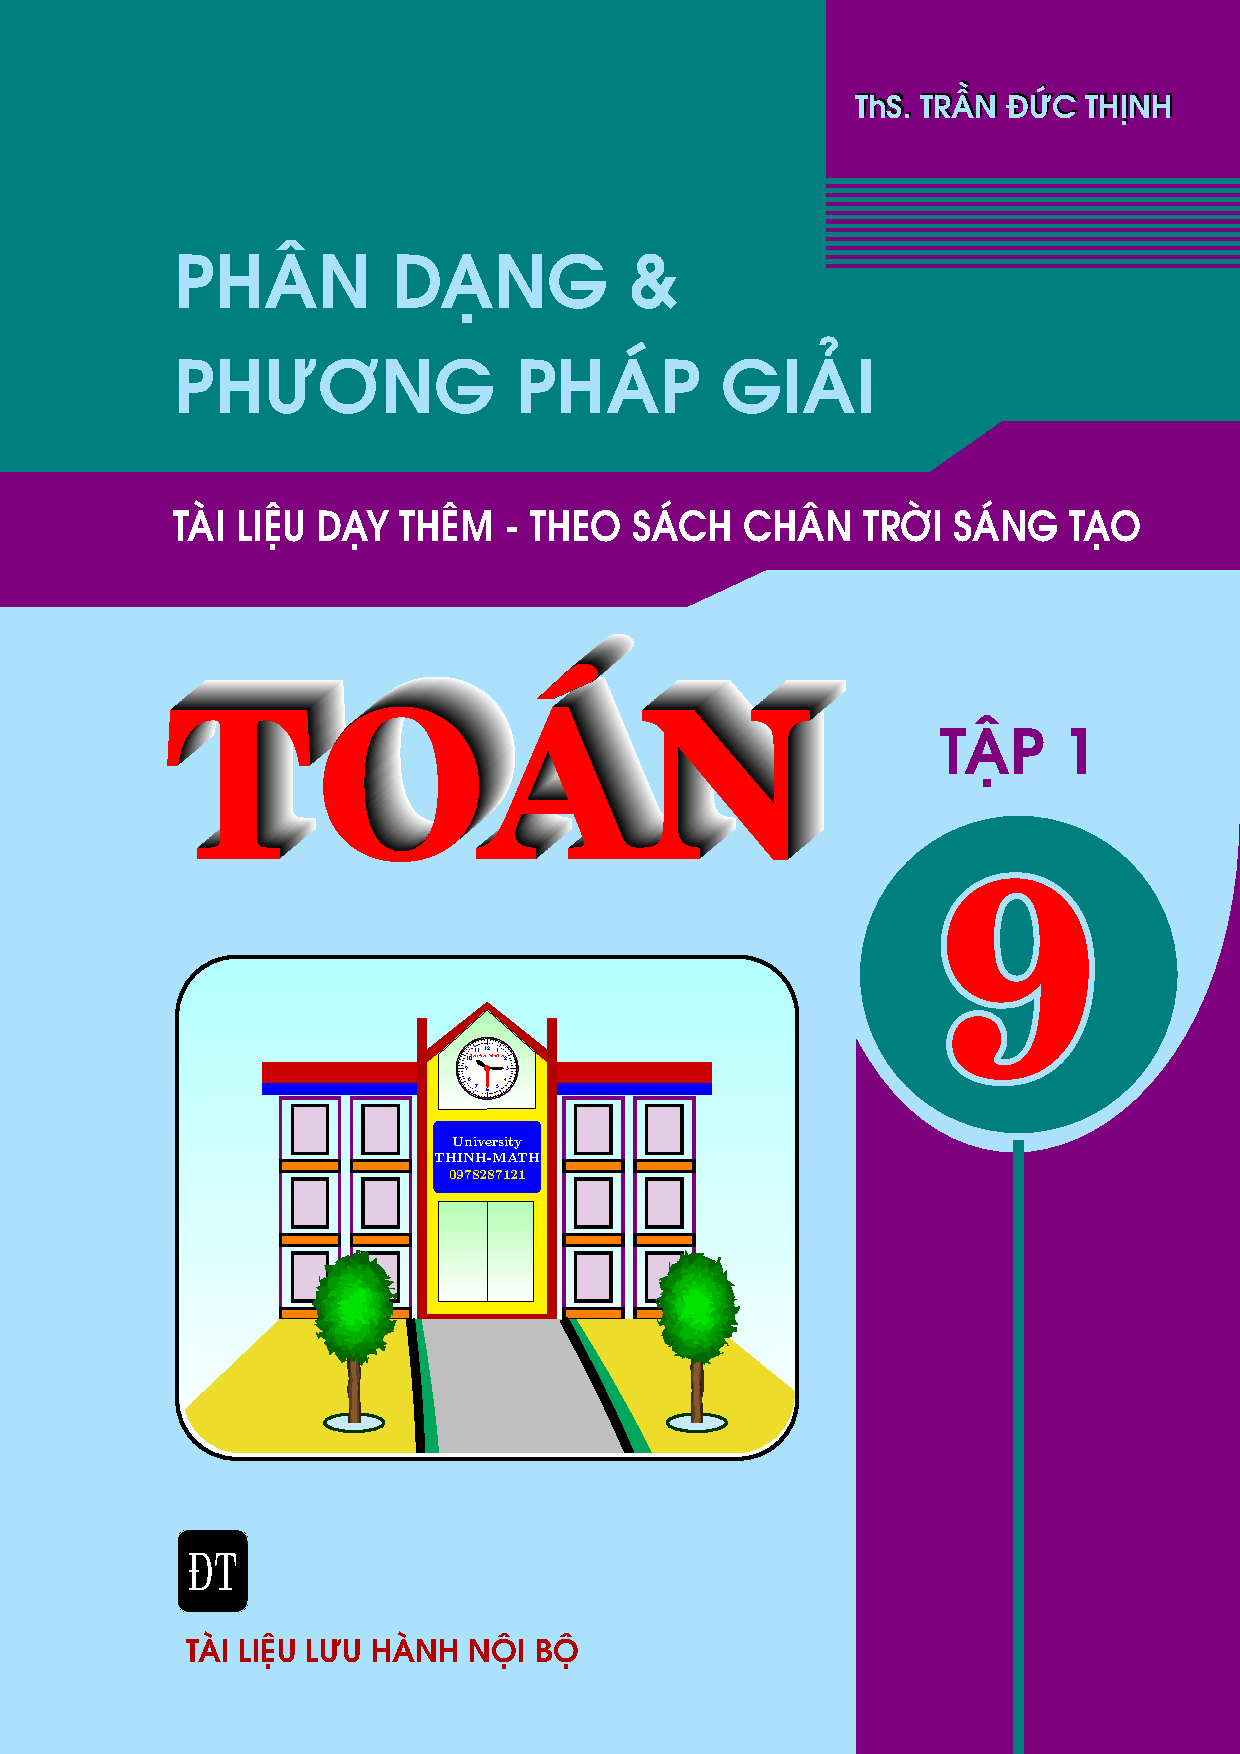
\includepdf{bia13/bia9-tap1-2.pdf}%chèn bìa pdf
%	\newpage\null\thispagestyle{empty}\newpage%tạo trang trống
	%--Mục lục chính
	\FULLWIDTH
	\muclucchinh
	%------------
	\clearpage%đặt lại đánh số trang
	\pagenumbering{arabic}%đánh số trang dạng 1,2,...
%====================================================
%==================BẮT ĐẦU TÀI LIỆU==================
%%%%\NOTE
%~~~~~~~~~~~~~~~~~~~~~~
\part{HỌC KÌ I}
%%%%%%%%%%%%%%%%%%% OKs
\setcounter{chapter}{0}  
\chapter{VẬT LÝ NHIỆT}
%\setcounter{section}{0}
\section{SỰ CHUYỂN THỂ}
\subsection{LÝ THUYẾT TRỌNG TÂM}
\subsubsection{Mô hình động học phân tử về cấu tạo chất}
\begin{boxdn}
	Mô hình động học phân tử về cấu tạo chất có những nội dung cơ bản sau:
	\begin{enumerate}[label=\arabic*.]
		\item Các chất được cấu tạo từ các hạt riêng biệt gọi là phân tử.
		\item Các phân tử chuyển động hỗn loạn, không ngừng. Nhiệt độ của vật càng cao thì tốc độ chuyển động của các phân tử cấu tạo nên vật càng lớn.
		\item Giữa các phân tử có lực hút và đẩy gọi chung là lực liên kết phân tử.
	\end{enumerate}
\end{boxdn}
\subsubsection{Cấu trúc của chất rắn, lỏng, khí}
\paragraph{Phân biệt cấu trúc của chất rắn, lỏng, khí}
\begin{center}
	\begin{tabular}{|p{4cm}|p{4cm}|p{4cm}|p{4cm}|}
		\hline
		\rowcolor{\nenVD}
		\thead{Đặc điểm}&\thead{Thể rắn} &\thead{Thể lỏng}&\thead{Thể khí}\\
		\hline
		Khoảng cách giữa các phân tử & Rất gần nhau (cỡ kích thước phân tử) & Xa nhau & Rất xa nhau (gấp hàng chục lần kích thước phân tử)\\
		\hline
		Lực tương tác phân tử & Rất mạnh & Nhỏ hơn trong chất rắn & Rất yếu\\
		\hline
		Sự sắp xếp của các phân tử & Trật tự & Kém trật tự hơn & Không có trật tự\\
		\hline
		Chuyển động của các phân tử & Chỉ dao động quanh vị trí cân bằng cố định & Dao động quanh vị trí cân bằng luôn luôn thay đổi & Chuyển động hỗn loạn \\
		\hline
		Hình dạng & Hình dạng riêng xác định & Có hình dạng của bình chứa & Có hình dạng của bính chứa\\
		\hline
		Thể tích & Xác định & Xác định & Chiếm toàn bộ thể tích bình chứa\\
		\hline
	\end{tabular}
\end{center}
\paragraph{Chất rắn kết tinh và chất rắn vô định hình}
\begin{boxdn}
	\begin{itemize}
		\item \textbf{Chất rắn kết tinh} là chất mà các hạt (phân tử, nguyên tử, ion) cấu tạo nên nó ở thể rắn, liên kết với nhau một cách chặt chẽ, sắp xếp theo một trật tự hình học xác định tạo thành các mạng tinh thể.
	\end{itemize}
\end{boxdn}
\begin{boxvidu}
\textit{\textbf{Ví dụ:}} muối ăn, thạch anh, kim cương, nước đá, \dots
\end{boxvidu}
	
	\begin{center}
		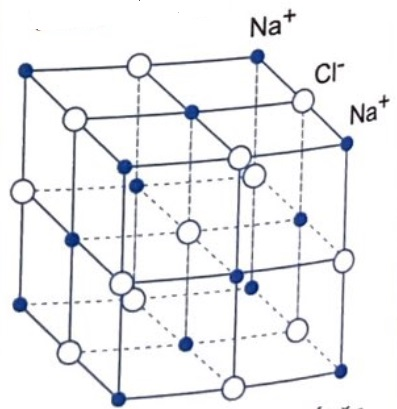
\includegraphics[width=0.2\linewidth]{figs/VN12-Y24-PH-SYL-001-3}
		\captionof{figure}{Cấu trúc tinh thể muối ăn}
	\end{center}
	\begin{boxdn}
		\begin{itemize}
		\item \textbf{Chất rắn vô định hình} là chất ở thể rắn mà các hạt tạo nên nó không tạo thành mạng tinh thể.\\
	\end{itemize}
	\end{boxdn}
\begin{boxvidu}
	\textbf{\textit{Ví dụ:}} thuỷ tinh, nhựa đường, sôcôla, \dots
\end{boxvidu}
\subsubsection{Sự chuyển thể}
\begin{boxdn}
	Khi các điều kiện như nhiệt độ, áp suất thay đổi, chất có thể chuyển từ thể này sang thể khác.
	\begin{itemize}
		\item Quá trình chuyển từ thể rắn sang thể lỏng của các chất được gọi là \textit{sự nóng chảy}. Quá trình ngược lại gọi là sự đông đặc.
		\item Quá trình chuyển từ thể lỏng sang thể khí (hơi) của các chất được gọi là \textit{sự hoá hơi}. Quá trình chuyển ngược lại gọi là sự ngưng tụ.
		\item Trong một số điều kiện, chất rắn có thể chuyển sang thể khí (hơi). Quá trình này gọi là sự thăng hoa. Quá trình ngược lại gọi là sự ngưng kết.\\
	\end{itemize}
\end{boxdn}
\begin{boxvidu}
	\textit{\textbf{Ví dụ:}} Sự thăng hoa dễ dàng của băng phiến ở nhiệt độ thường. Sự ngưng kết của hơi nước trong không khí tạo thành sương muối.
\end{boxvidu}
	\begin{center}
		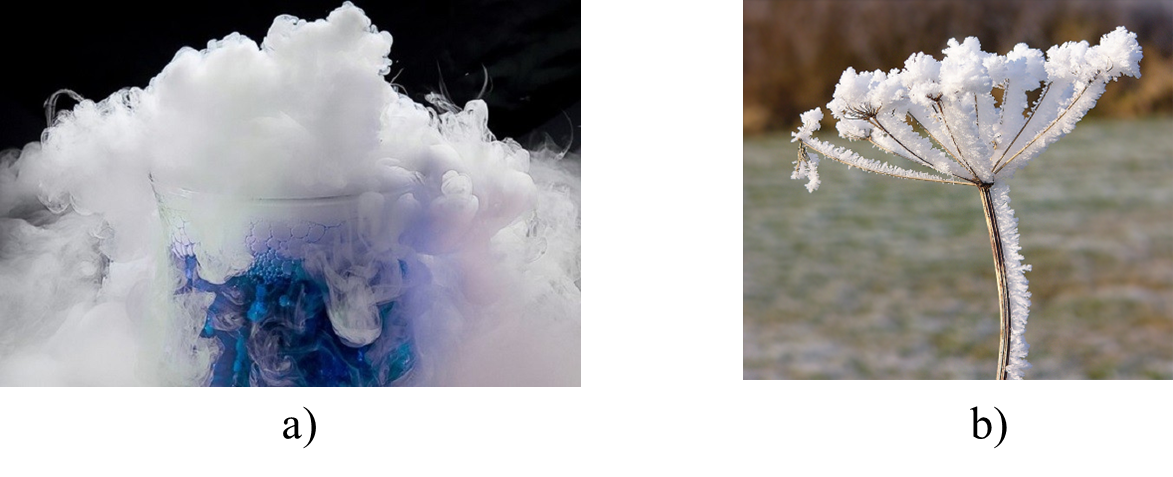
\includegraphics[width=0.7\linewidth]{figs/VN12-Y24-PH-SYL-001-7}
		\captionof{figure}{a) Đá khô thăng hoa; b) Sương muối}
	\end{center}

\begin{center}
	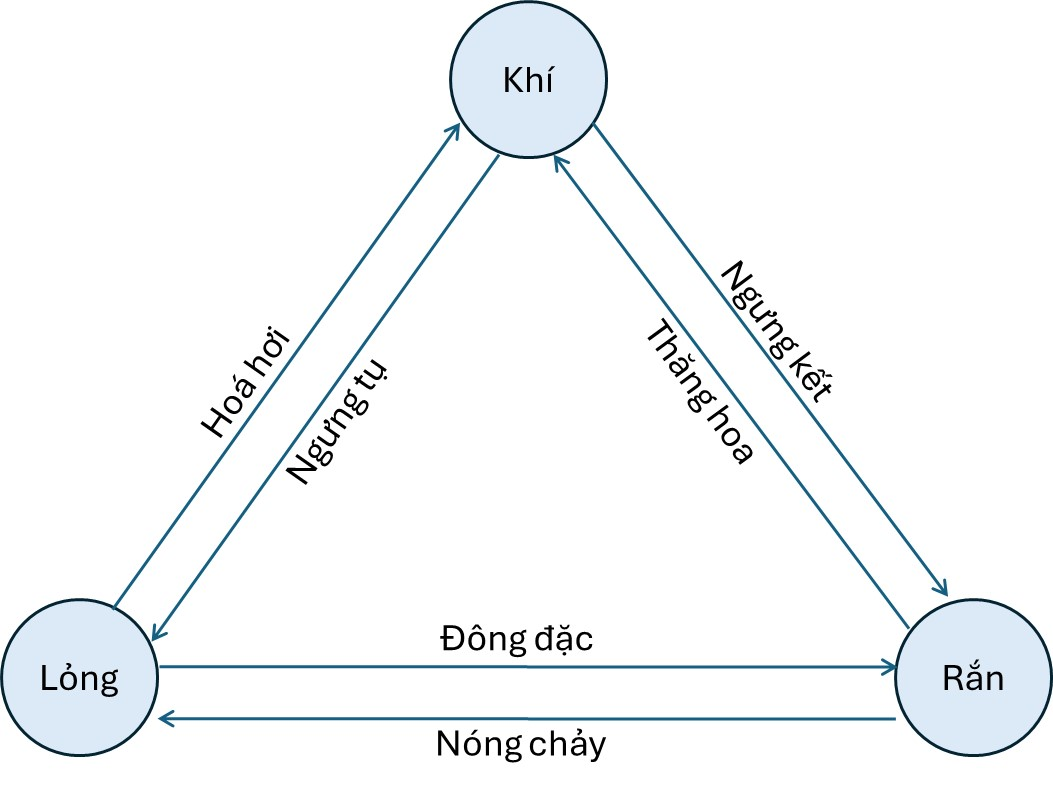
\includegraphics[width=0.5\linewidth]{figs/VN12-Y24-PH-SYL-001-4}
	\captionof{figure}{Sơ đồ các hình thức chuyển thể}
\end{center}
\paragraph{Sự nóng chảy}
\begin{boxdn}
	Khi đun nóng đến một nhiệt độ nào đó, vật rắn bắt đầu chuyển trạng thái từ rắn sang lỏng (sự nóng chảy). Chất rắn kết tinh có nhiệt độ nóng chảy xác định (ở một áp suất cụ thể). Chất rắn vô định hình không có nhiệt độ nóng chảy xác định.\\
\end{boxdn}
\begin{boxvidu}
	\textbf{\textit{Ví dụ:}}
	\begin{itemize}
		\item Khi nung nóng nước đá ở áp suất tiêu chuẩn, nhiệt độ nước đá tăng dần. Khi đạt đến $\SI{0}{\celsius}$, nước đá bắt đầu tan và trong suốt quá trình hoá lỏng nhiệt độ của nước đá không đổi. Nước đá là chất rắn kết tinh.
		\item Khi nung nóng thỏi sôcôla, thỏi sôcôla mềm đi và chuyển dần sang thể lỏng, trong quá trình này nhiệt độ của thỏi sôcôla vẫn tăng liên tục. Thỏi sôcôla là chất rắn vô định hình.
	\end{itemize}
	\begin{center}
		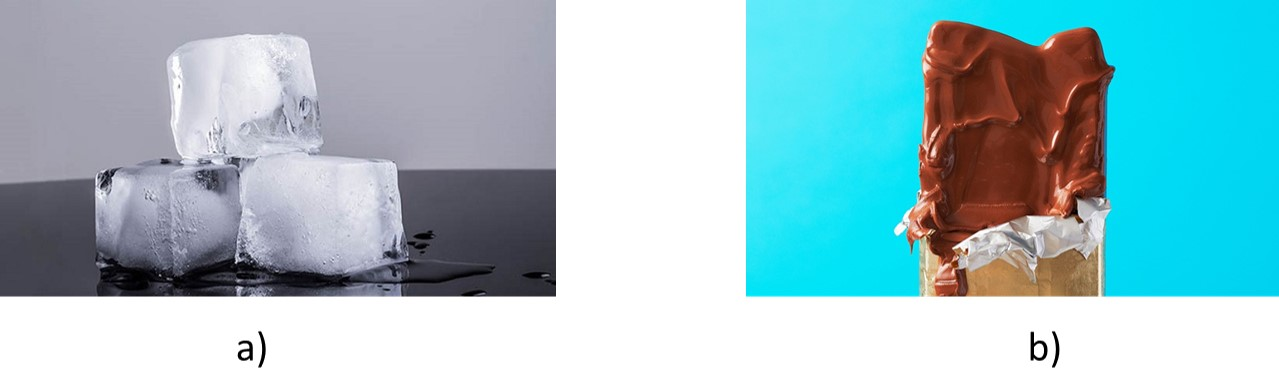
\includegraphics[width=0.6\linewidth]{figs/VN12-Y24-PH-SYL-001-5}
		\captionof{figure}{a) Nước đá đang tan; b) Thanh sôcôla đang nóng chảy}
	\end{center}
\end{boxvidu}
\paragraph{Sự hoá hơi}
\begin{boxdn}
	\begin{itemize}
		\item \textbf{Sự bay hơi}\\
		Sự bay hơi là sự hoá hơi xảy ra \textbf{trên bề mặt chất lỏng}. Sự bay hơi xảy ra ở \textbf{nhiệt độ bất kì}.\\
		Tốc độ bay hơi của chất lỏng càng nhanh nếu diện tích mặt thoáng càng lớn, tốc độ gió càng lớn, nhiệt độ càng cao, và độ ẩm không khí càng thấp.
		\item \textbf{Sự sôi}\\
		Sự sôi là sự hoá hơi xảy ra \textbf{bên trong và trên bề mặt chất lỏng}. Sự sôi xảy ra ở \textbf{nhiệt độ sôi}.\\
		Nhiệt độ sôi của chất lỏng phụ thuộc áp suất khí trên mặt thoáng và bản chất của chất lỏng. Trong suốt thời gian sôi, nhiệt độ của chất lỏng không thay đổi.
	\end{itemize}
\end{boxdn}
\begin{center}
	
	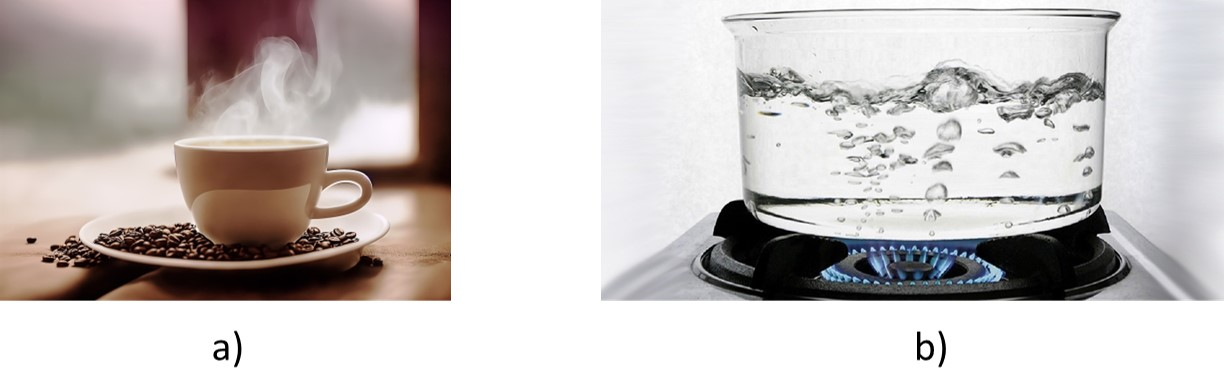
\includegraphics[width=0.65\linewidth]{figs/VN12-Y24-PH-SYL-001-6}
	\captionof{figure}{a) Nước bay hơi trên mặt thoáng của tách cà phê; b) Nước đang sôi}
\end{center}
\subsection{VÍ DỤ MINH HOẠ}
\begin{dang}{Sử dụng mô hình động học phân tử, nêu được sơ lược cấu trúc của chất rắn, chất lỏng, chất khí}
\end{dang}
\begin{vd}
	Năm 1827, khi làm thí nghiệm quan sát các hạt phấn hoa rất nhỏ trong nước bằng kính hiển vi, Brown thấy chúng chuyển động hỗn loạn, không ngừng. Chuyển động này được gọi là chuyển động Brown.\\
	\begin{center}
		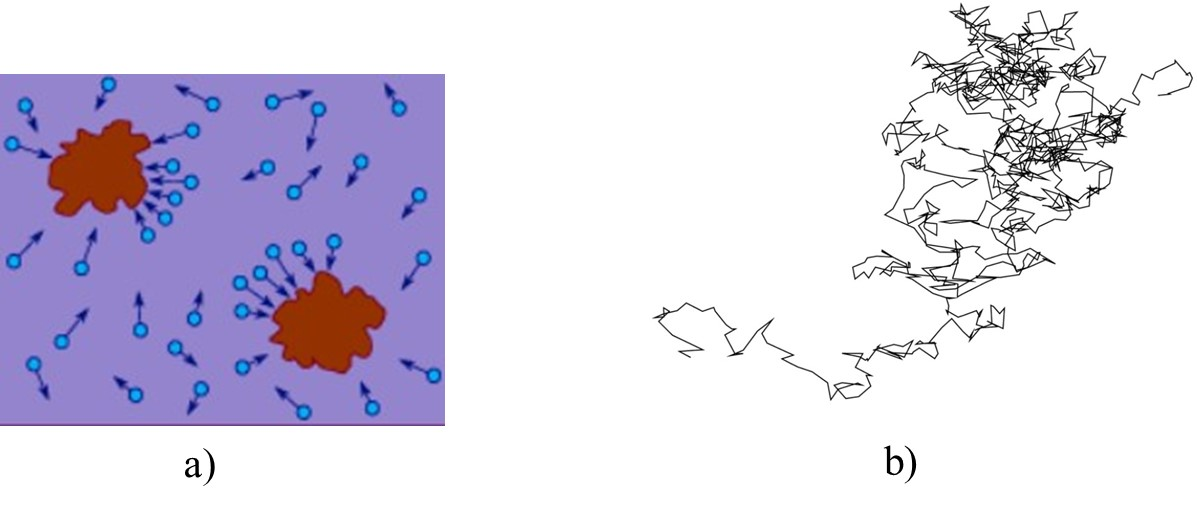
\includegraphics[width=0.6\linewidth]{figs/VN12-Y24-PH-SYL-001-1}
		\captionof{figure}{a) Mô phỏng sự va chạm giữa các phân tử nước với các hạt phấn hoa; b) Quỹ đạo chuyển động của hạt phấn hoa}
	\end{center}
	\begin{enumerate}[label=\alph*)]
		\item Tại sao thí nghiệm của Brown được gọi là một trong những thí nghiệm chứng tỏ các phân tử chuyển động hỗn loạn không ngừng?
		\item Làm thế nào để với thí nghiệm của Brown có thể chứng tỏ được khi nhiệt độ của nước càng cao thì các phân tử nước chuyển động càng nhanh?
	\end{enumerate}
	\loigiai{
		\begin{enumerate}[label=\alph*)]
			\item Thông qua việc quan sát hạt phấn hoa trong nước, Brown nhận thấy rằng các hạt phấn hoa lắc lư không ngừng và quỹ đạo chuyển động của hạt phấn hoa hỗn loạn. Mà chuyển động của hạt phấn hoa là do sự va chạm  giữa các phân tử nước với hạt phấn hoa gây ra. Điều này chứng tỏ rằng chuyển động của các phân tử nước cũng hỗn loạn, không ngừng.
			\item Để với thí nghiệm của Brown có thể chứng tỏ được khi nhiệt độ của nước càng cao thì các phân tử nước chuyển động càng nhanh thì chúng ta có thể đun nóng nước rồi quan sát sự thay đổi tốc độ chuyển động của hạt phấn hoa.
	\end{enumerate}}
\end{vd}
\begin{vd}
	Hãy giải thích đặc điểm sau đây của thể khí, thể rắn, thể lỏng.
	\begin{enumerate}[label=\alph*)]
		\item Chất khí không có hình dạng và thể tích riêng, luôn chiếm toàn bộ thể tích bình chứa và có thể nén được dễ dàng.
		\item Vật ở thể rắn có thể tích và hình dạng riêng, rất khó nén.
		\item Vật ở thể lỏng có thể tích riêng nhưng không có hình dạng riêng.
	\end{enumerate}
	\loigiai{
		\begin{enumerate}[label=\alph*)]
			\item Ở thể khí, các phân tử ở xa nhau (khoảng cách giữa các phân tử lớn gấp hàng chục lần kích thước phân tử). Lực tương tác giữa các phân tử rất yếu (trừ trường hợp chúng va chạm nhau) nên các phân tử chuyển động hoàn toàn hỗn loạn. Do đó, khối chất khí không có hình dạng và thể tích riêng mà có hình dạng và thể tích của bình chứa nó.
			\item Ở thể rắn, các phân tử rất gần nhau (khoảng cách giữa các phân tử cỡ kích thước phân tử) và các phân tử sắp xếp có trật tự, chặt chẽ. Lực tương tác giữa các phân tử rất mạnh, giữ cho chúng không di chuyển tự do mà chỉ có thể dao động quanh vị trí cân bằng xác định. Do đó, vật rắn luôn có thể tích và hình dạng riêng xác định, đồng thời rất khó nén.
			\item Khoảng cách giữa các phân tử trong chất lỏng lớn hơn khoảng cách giữa các phân tử trong chất rắn và nhỏ hơn khoảng cách giữa các phân tử trong chất khí. Lực tương tác giữa các phân tử ở thể lỏng lớn hơn lực tương tác giữa các phân tử ở thể khí nên giữ các phân tử không bị phân tán ra xa nhau, do đó chất lỏng có thể tích riêng xác định. Lực tương tác này chưa đủ lớn như trong thể rắn nên các phân tử ở thể lỏng cũng dao động quanh vị trí cân bằng nhưng các vị trí cân bằng này luôn luôn thay đổi. Do đó, khối chất lỏng không có hình dạng riêng xác định mà có hình dạng của bình chứa nó.
	\end{enumerate}}
\end{vd}

\begin{dang}{Giải thích được sơ lược một số hiện tượng vật lí liên quan đến sự chuyển thể: sự nóng chảy, sự hoá hơi}
\end{dang}
%\setcounter{vd}{0}
\begin{vd}
	Vận dụng mô hình động học phân tử, em hãy giải thích nguyên nhân gây ra sự nóng chảy của chất rắn kết tinh.
	\loigiai{
		Ở áp suất không đổi, các phân tử ở thể rắn liên kết chặt chẽ với nhau, chúng dao động quanh các vị trí cân bằng xác định. Khi nung nóng chất rắn kết tinh, các phân tử được cung cấp nhiệt năng làm tốc độ chuyển động nhiệt của nó tăng lên, mức độ trật tự trong cấu trúc của các hạt giảm đi.  Điều này dẫn đến khoảng cách trung bình giữa các phân tử tăng.\\
		Nhiệt độ của vật rắn tăng đến một giá trị nào đó thì một số phân tử thắng được lực liên kết với các phân tử xung quanh và thoát khỏi liên kết với chúng, đó là sự khởi đầu của quá trình nóng chảy. Từ lúc này, vật rắn nhận nhiệt lượng để tiếp tục phá vỡ các liên kết tinh thể. Khi trật tự của tinh thể bị phá vỡ hoàn toàn thì quá trình nóng chảy kết thúc, vật rắn chuyển thành khối chất lỏng.
	}
\end{vd}
\begin{vd}
	Vận dụng mô hình động học phân tử, em hãy giải tích nguyên nhân gây ra sự bay hơi và sự sôi.

\loigiai{\begin{itemize}
		\item \textbf{Giải thích sự bay hơi:}\\
		Các phân tử ở bề mặt chất lỏng tham gia chuyển động nhiệt, trong đó có những phân tử chuyển động hướng ra ngoài chất lỏng. Đồng thời, các phân tử có thể truyền năng lượng cho nhau thông qua quá trình va chạm. Do đó, một số phân tử ở gần mặt thoáng của chất lỏng có động năng đủ lớn để thắng lực liên kết của các phân tử chất lỏng khác thì thoát được ra khỏi mặt thoáng của chất lỏng trở thành các phân tử ở thể hơi.
		\item \textbf{Giải thích sự sôi:}\\
		Khi chất lỏng đến nhiệt độ sôi, do tiếp tục được cung cấp nhiệt nên các phân tử chất lỏng chuyển động nhiệt mạnh hơn, làm phá vỡ sự liên kết giữa các phân tử chất lỏng với nhau. Khi đó các bọt chứa không khí và hơi nước nổi lên trong lòng nước càng ngày càng nhiều, càng nổi lên trên thể tích các bọt khí này càng tăng, tới mặt thoáng thì vỡ, không khí và hơi nước thoát ra ngoài khí quyển.
\end{itemize}}
\end{vd}


\subsection{BÀI TẬP TRẮC NGHIỆM}

\Opensolutionfile{ans}[ans/G12Y24B1TN]
\begin{ex}
Chuyển động của các nguyên tử, phân tử trong mô hình động học phân tử được gọi là chuyển động
\choice
{chuyển động cơ}
{\True chuyển động nhiệt}
{chuyển động tròn}
{chuyển động đều}
\loigiai{ }
\end{ex}

%==============================================
\begin{ex}

Chọn phát biểu \textbf{đúng} về lực tương tác giữa các phân tử.
\choice
{\True Giữa các phân tử có cả lực hút và lực đẩy}
{ Giữa các phân tử chỉ có lực hút hoặc lực đẩy}
{ Giữa các phân tử chỉ có lực đẩy}
{ Giữa các phân tử chỉ có lực hút}
\loigiai{ }
\end{ex}

%==============================================
\begin{ex}
Khi khoảng cách giữa các phân tử rất nhỏ, thì giữa các phân tử
\choice
{ chỉ có lực hút}
{ chỉ có lực đẩy}
{\True có cả lực hút và lực đẩy, nhưng lực đẩy lớn hơn lực hút}
{ có cả lực hút và lực đẩy, nhưng lực đẩy nhỏ hơn lực hút}
\loigiai{ }
\end{ex}


%==============================================
\begin{ex}
Mục đích của thí nghiệm Brown là
\choice
{ quan sát hạt phấn hoa bằng kính hiển vi}
{\True quan sát chuyển động của hạt phấn hoa trong nước bằng kính hiển vi}
{ quan sát cánh hoa trong nước bằng kính hiển vi}
{ quan sát chuyển động của cánh hoa}
\loigiai{ }
\end{ex}


%==============================================
\begin{ex} 
Trong thí nghiệm của Brown các hạt phấn hoa chuyển động hỗn độn, không ngừng vì
\choice
{ giữa các hạt phấn hoa có lực tương tác hút và đẩy}
{ các hạt phấn hoa là các thực thể sống}
{\True các phân tử nước chuyển động không ngừng, va chạm vào chúng từ mọi phía}
{ các hạt phấn hoa có thể dao động tự do quanh vị trí cân bằng}
\loigiai{ }
\end{ex}


%==============================================
\begin{ex}
Chọn câu trả lời \textbf{đúng nhất}. \\
Các chất có thể tồn tại ở những thể nào?
\choice
{ Thể rắn, thể lỏng, thể khí hoặc chân không}
{\True Thể rắn, thể lỏng hoặc thể khí}
{ Thể rắn và thể hơi}
{ Thể rắn và thế lỏng}
\loigiai{ }
\end{ex}


%==============================================
\begin{ex}
Đặc điểm nào sau đây là phù hợp với chất rắn?
\choice
{\True Có lực tương tác giữa các phân tử rất mạnh}
{ Có lực tương tác giữa các phân tử rất yếu}
{ Không có hình dạng xác định}
{ Không có thể tích riêng xác định}
\loigiai{ }
\end{ex}


%==============================================
\begin{ex}
Phát biểu nào dưới đây là đúng khi nói về những đặc điểm của chất rắn?
\choice
{ Có khối lượng, hình dạng xác định, không có thể tích xác định}
{ Có khối lượng xác định, hình dạng và thể tích không xác định}
{\True Có khối lượng, hình dạng, thể tích xác định}
{ Có khối lượng và thể tích xác định, hình dạng không xác định}
\loigiai{ }
\end{ex}


%==============================================
\begin{ex}
Người ta có thể phân loại chất rắn một cách tổng quát theo cách nào sau đây?
\choice
{ Chất rắn đơn tinh thể và chất rắn vô định hình}
{\True Chất rắn kết tinh và chất rắn vô định hình}
{ Chất rắn đa tinh thể và chất rắn vô định hình}
{ Chất rắn đơn tinh thể và chất rắn đa tinh thể}
\loigiai{ }
\end{ex}


%==============================================
\begin{ex} 
Đặc điểm nào sau đây là đặc điểm cấu trúc phân tử ở thể lỏng?
\choice
{ Khoảng cách giữa các phân tử rất lớn so với kích thước của chúng}
{\True Lực tương tác phân tử yếu hơn lực tương tác phân tử ở thể rắn}
{ Không có thể tích và hình dạng riêng xác định}
{ Các phân tử dao động xung quanh vị trí cân bằng xác định}
\loigiai{ }
\end{ex}


%==============================================
\begin{ex} 
Trong chuyển động nhiệt, các phân tử chất lỏng
\choice
{ dao động quanh vị trí cân bằng xác định}
{ chuyển động hỗn loạn quanh vị trí cân bằng xác định}
{ chuyển động hỗn loạn}
{\True dao động quanh vị trí cân bằng nhưng những vị trí này không cố định mà luôn thay đổi}
\loigiai{ }
\end{ex}


%==============================================
\begin{ex}
Chất lỏng có thể tích xác định, nhưng hình dạng không xác định là do trong chất lỏng
\choice
{ lực liên kết giữa các phân tử chất lỏng là rất lớn, các phân tử chỉ dao động không ngừng quanh một vị trí xác định}
{ lực liên kết giữa các phân tử chất lỏng là rất yếu, các phân tử dao động tự do về mọi phía}
{\True lực liên kết giữa các phân tử chất lỏng là yếu hơn chất rắn, các phân tử dao động tương đối tự do hơn so với trong chất rắn}
{ Tất cả các phương án đưa ra đều sai}
\loigiai{ }
\end{ex}


%==============================================
\begin{ex} 
Các phân tử khí chuyển động hỗn loạn, không ngừng vì
\choice
{ phân tử khí không có khối lượng}
{ khoảng cách giữa các phân tử khí quá gần nhau}
{\True lực tương tác giữa các phân tử quá nhỏ}
{ các phân tử khí luôn đẩy nhau}
\loigiai{ }
\end{ex}


%==============================================
\begin{ex}
Tính chất nào sau đây \textbf{không phải} là tính chất của chất ở thể khí?
\choice
{\True Có hình dạng và thể tích riêng}
{ Có các phân tử chuyển động hoàn toàn hỗn độn}
{ Có thể nén được dễ dàng}
{ Có lực tương tác phân tử nhỏ hơn lực tương tác phân tử ở thể rắn và thể lỏng}
\loigiai{ }
\end{ex}


%==============================================
\begin{ex}
Chất khí không có hình dạng và thể tích riêng là vì
\choice
{ khoảng cách giữa các phân tử rất gần, lực tương tác giữa các phân tử chất khí rất mạnh}
{ khoảng cách giữa các phân tử rất gần, lực tương tác giữa các phân tử chất khí rất yếu}
{ khoảng cách giữa các phân tử rất xa, lực tương tác giữa các phân tử chất khí rất mạnh}
{\True khoảng cách giữa các phân tử rất xa, lực tương tác giữa các phân tử chất khí rất yếu}
\loigiai{ }
\end{ex}


%==============================================
\begin{ex}
Khi mở nắp lọ nước hoa, ta có thể ngửi thấy mùi thơm tràn ngập trong phòng. Điều này thể hiện tính chất nào của chất khí?
\choice
{ Dễ dàng nén được}
{ Có khối lượng xác định}
{\True Có thể khuếch tán trong không gian theo mọi hướng}
{ Không chảy được}
\loigiai{ }
\end{ex}


%==============================================
\begin{ex}
Sự nóng chảy là
\choice
{\True sự chuyển thế từ rắn sang lỏng}
{ sự chuyển thể từ rắn sang khí}
{ sự chuyển thể từ lỏng sang rắn}
{ sự chuyển thể từ lỏng sang khí}
\loigiai{ }
\end{ex}


%==============================================
\begin{ex}
Sự đông đặc là
\choice
{ sự chuyển thế từ rắn sang lỏng}
{ sự chuyển thể từ rắn sang khí}
{\True sự chuyển thể từ lỏng sang rắn}
{ sự chuyển thể từ lỏng sang khí}
\loigiai{ }
\end{ex}
%==============================================
\begin{ex}
Sự bay hơi là
\choice
{ sự chuyển thế từ rắn sang lỏng}
{ sự chuyển thể từ rắn sang khí}
{ sự chuyển thể từ lỏng sang rắn}
{\True sự chuyển thể từ lỏng sang khí}
\loigiai{ }
\end{ex}
%==============================================
\begin{ex}
Khi quan sát sự nóng chảy của nước đá, trong suốt thời gian nóng chảy thì
\choice
{ nhiệt độ của nước đá tăng}
{ nhiệt độ của nước đá giảm}
{\True nhiệt  độ của nước đá không đổi}
{ nhiệt độ của nước đá ban đầu tăng và sau đó giảm}
\loigiai{ }
\end{ex}
%==============================================
\begin{ex}
Phát biểu nào sau đây về tính chất của chất rắn kết tinh và chất rắn vô định hình là \textbf{đúng}?
\choice
{ Chất rắn kết tinh và chất rắn vô định hình đều có nhiệt độ nóng chảy xác định}
{ Chất rắn kết tinh không có nhiệt độ nóng chảy xác định, chất rắn vô định hình có nhiệt độ nóng chảy xác định}
{\True Chất rắn kết tinh có nhiệt độ nóng chảy xác định, chất rắn vô định hình không có nhiệt độ nóng chảy xác định}
{ Chất rắn kết tinh và chất rắn vô định hình đều không có nhiệt độ nóng chảy xác định}
\loigiai{ }
\end{ex}
%==============================================
\begin{ex}
Một vật rắn khi bị nung nóng thì mềm dần. Đó là
\choice
{ chất rắn kết tinh}
{ chất rắn đơn tinh thể}
{ chất rắn đa tinh thể}
{\True chất rắn vô định hình}
\loigiai{ }
\end{ex}
%==============================================
\begin{ex}
Trường hợp nào sau đây không liên quan đến sự nóng chảy và đông đặc?
	\begin{center}
		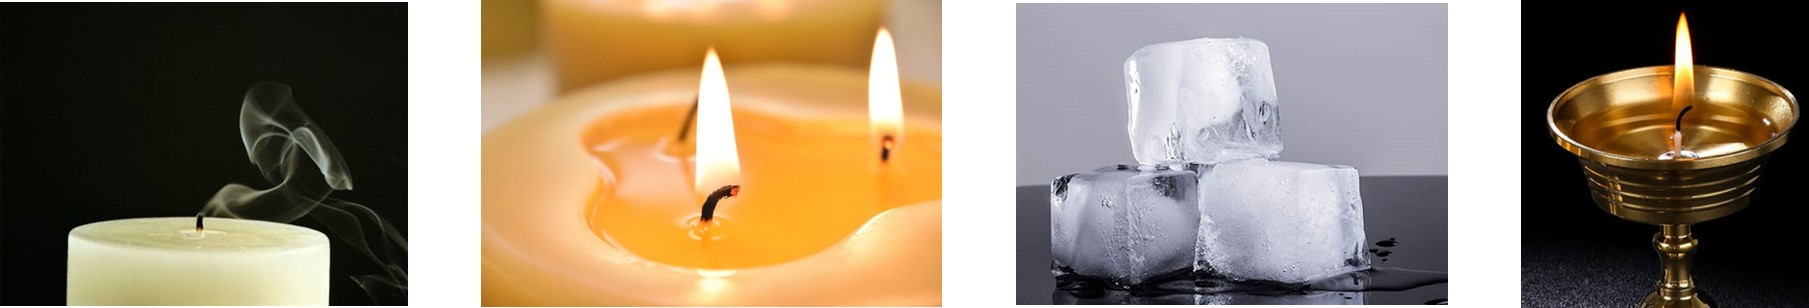
\includegraphics[width=0.45\linewidth]{figs/VN12-Y24-PH-SYL-001P-2}
	\end{center}
\choice
{ Ngọn nến vừa tắt}
{ Ngọn nến đang cháy}
{ Nước đá vừa lấy ra khỏi tủ lạnh}
{\True Ngọn đèn dầu đang cháy}
\loigiai{ }
\end{ex}
%==============================================
\begin{ex}
Sự bay hơi diễn ra càng nhanh hơn khi
\choice
{ nhiệt độ càng thấp}
{\True tốc độ gió càng lớn}
{ lượng chất lỏng càng nhiều}
{ diện tích mặt thoáng càng hẹp}
\loigiai{ }
\end{ex}
%==============================================
\begin{ex}
Một ấm nước đang sôi, nếu tiếp tục đun thì
\choice
{ nhiệt độ nước trong ấm giảm xuống}
{ nước trong ấm không bay hơi nữa}
{ nhiệt độ nước trong ấm vẫn tiếp tục tăng}
{\True nước trong ấm bay hơi nhiều hơn và cạn dần}
\loigiai{ }
\end{ex}
%==============================================
\begin{ex}
Phát biểu nào sau đây là \textbf{không đúng} về sự bay hơi?
\choice
{ Sự bay hơi là quá trình chuyển từ thể lỏng sang thể khí xảy ra ở bề mặt chất lỏng}
{\True Sự bay hơi là quá trình chuyển từ thể lỏng sang thể khí xảy ra ở cả bên trong và trên bề mặt chất lỏng}
{ Sự bay hơi của chất lỏng xảy ra ở nhiệt độ bất kì}
{ Sự ngưng tụ luôn kèm theo sự bay hơi}
\loigiai{ }
\end{ex}
%==============================================
\begin{ex}
Sự sôi xảy ra ở
\choice
{ nhiệt độ trên $\SI{100}{\celsius}$}
{ $\SI{100}{\celsius}$}
{\True nhiệt độ sôi}
{ dưới $\SI{100}{\celsius}$}
\loigiai{ }
\end{ex}
%==============================================
\begin{ex}
Trong các trường hợp dưới đây, trường hợp nào liên quan đến sự bay hơi?
\choice
{ Kính cửa sổ bị mờ đi trong những ngày đông giá lạnh}
{\True Dầu trong đèn bị khô cạn dù không sử dụng}
{ Miếng bơ để bên ngoài tủ lạnh sau một thời gian bị chảy lỏng}
{ Đưa nước vào trong tủ lạnh để làm đá}
\loigiai{ }
\end{ex}
%==============================================
\begin{ex}
Tại sao quả bóng bay dù buộc chặt để lâu ngày vẫn bị xẹp?
\choice
{ Vì khi mới thổi, không khí từ miệng vào bóng còn nóng, sau đó lạnh dần nên co lại}
{ Vì cao su là chất đàn hồi nên sau khi bị thổi căng nó tự động co lại}
{ Vì không khí nhẹ nên có thể chui qua chỗ buộc ra ngoài}
{\True Vì giữa các phân tử của chất làm vỏ bóng có khoảng cách nên các phân tử không khí có thể chui qua đó và thoát ra ngoài}
\loigiai{ }
\end{ex}
%==============================================
\begin{ex}
Hãy chọn phương án \textbf{sai}.\\
Cùng một khối lượng của một chất nhưng khi ở các thể khác nhau thì sẽ khác nhau
\choice
{ Thể tích}
{ Khối lượng riêng}
{\True Kích thước của các nguyên tử}
{ Trật tự của các nguyên tử}
\loigiai{ }
\end{ex}
%==============================================
\begin{ex}
Các nguyên tử trong một miếng sắt có tính chất nào sau đây?
\choice
{ Khi nhiệt độ tăng thì nở ra}
{ Khi nhiệt độ giảm thì co lại}
{\True Đứng rất gần nhau}
{ Đứng xa nhau}
\loigiai{ }
\end{ex}
%==============================================
\begin{ex}
Trong các chất sau, chất nào \textbf{không phải} là chất rắn kết tinh?
\choice
{ Muối ăn}
{\True Thuỷ tinh}
{ Kim cương}
{ Thạch anh}
\loigiai{ }
\end{ex}
%==============================================
\begin{ex}
Chất rắn nào dưới đây không phải là chất rắn vô định hình?
\choice
{\True Thạch anh}
{ Thuỷ tinh}
{ Sáp}
{ Cao su}
\loigiai{ }
\end{ex}
%==============================================
\begin{ex}
Chất rắn nào dưới đây là chất rắn vô định hình?
\choice
{ Muối ăn}
{ Kim loại}
{ Thạch anh}
{\True Nhựa đường}
\loigiai{ }
\end{ex}
%==============================================
\begin{ex}
Ở điều kiện thường, iode là chất rắn dạng tinh thể màu đen tím. Khi đun nóng, iode có sự thăng hoa.\\
Vậy sự thăng hoa của iode là sự chuyển trạng thái từ thể
\choice
{\True rắn sang khí}
{ rắn sang lỏng}
{ lỏng sang rắn}
{ khí sang rắn}
\loigiai{ }
\end{ex}
%==============================================
\begin{ex}
Cho đồ thị biểu diễn sự thay đổi nhiệt độ theo thời gian của nước đá như hình vẽ. Nước đá tan trong khoảng thời gian nào?
\begin{center}
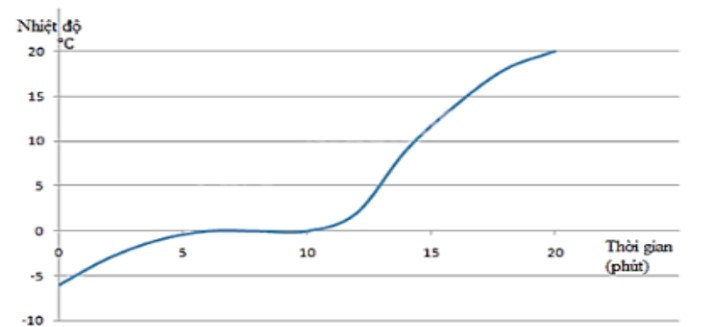
\includegraphics[width=0.6\linewidth]{figs/VN12-Y24-PH-SYL-001P-1}
\end{center}
\choice
{\True Từ phút thứ 6 đến phút thứ 10}
{ Từ phút thứ 10 trở đi}
{ Từ 0 đến phút thứ 6}
{ Từ phút thứ 10 đến phút thứ 15}
\loigiai{ }
\end{ex}
%==============================================
\begin{ex}
Người ta không thể luộc trứng chín ở núi cao vì
\choice
{\True áp suất trên núi thấp hơn áp suất chuẩn $\left(\SI{1}{atm}\right)$ nên nước sôi ở nhiệt độ thấp hơn $\SI{100}{\celsius}$}
{ áp suất trên núi cao hơn áp suất chuẩn $\left(\SI{1}{atm}\right)$ nên nước sôi ở nhiệt độ thấp hơn $\SI{100}{\celsius}$}
{ áp suất trên núi thấp hơn áp suất chuẩn $\left(\SI{1}{atm}\right)$ nên nước sôi ở nhiệt độ cao hơn $\SI{100}{\celsius}$}
{ áp suất trên núi cao hơn áp suất chuẩn $\left(\SI{1}{atm}\right)$ nên nước sôi ở nhiệt độ cao hơn $\SI{100}{\celsius}$}
\loigiai{ }
\end{ex}
%==============================================
\begin{ex}
Thuỷ ngân có nhiệt độ nóng chảy là $\SI{-39}{\celsius}$ và nhiệt độ sôi là $\SI{357}{\celsius}$. Khi ở trong phòng có nhiệt độ $\SI{30}{\celsius}$ thì thuỷ ngân
\choice
{\True chỉ tồn tại ở thể lỏng}
{ chỉ tồn tại ở thể hơi}
{ tồn tại ở cả thể lỏng và thể hơi}
{ tồn tại ở cả thể rắn, lỏng và hơi}
\loigiai{ }
\end{ex}
%==============================================
\begin{ex}
Tại sao khi cầm vào vỏ bình ga mini đang sử dụng ta thường thấy có một lớp nước rất
mỏng trên đó?
\choice
{ Do hơi nước từ tay ta bốc ra}
{ Nước từ trong bình ga thấm ra}
{\True Do vỏ bình ga lạnh hơn nhiệt độ môi trường nên hơi nước trong không khí ngưng tụ trên đó}
{ Cả B và C đều đúng}
\loigiai{ }
\end{ex}
%==============================================
\begin{ex}
Ở nhiệt độ trong phòng, chỉ có thể có khí oxygen, không thể có oxygen lỏng vì
\choice
{ oxygen luôn là chất khí}
{\True nhiệt độ phòng cao hơn nhiệt độ sôi của oxygen}
{ nhiệt độ phòng thấp hơn nhiệt độ sôi của oxygen}
{ nhiệt độ trong phòng bằng nhiệt độ sôi của oxygen}
\loigiai{ }
\end{ex}

\Closesolutionfile{ans}

\subsection{TRẮC NGHIỆM ĐÚNG/SAI}
\Opensolutionfile{ans}[ans/G12Y24B1DS]
\setcounter{ex}{0}
\begin{ex}
	Nhận định các phát biểu sau đây về mô hình động học phân tử.
	\begin{enumerate}[label=\alph*)]
		\item Các chất được cấu tạo từ các hạt riêng biệt được gọi nguyên tử, phân tử.
		\item Các nguyên tử, phân tử đứng sát nhau và giữa chúng không có khoảng cách.
		\item Lực tương tác giữa các phân tử ở thể rắn lớn hơn lực tương tác giữa các phân tử ở thể lỏng và thể khí.
		\item Các nguyên tử, phân tử chất lỏng dao động xung quanh các vị trí cân bằng không cố định.
	\end{enumerate}
\loigiai{
\begin{enumerate}[label=\alph*)]
	\item Đúng.
	\item Sai.
	\item Đúng.
	\item Đúng.
\end{enumerate}
}
	\end{ex}
%=====================================================================================
\begin{ex}
	Nhận định các phát biểu về sự sôi.
	\begin{enumerate}[label=\alph*)]
		\item Nước chỉ sôi ở nhiệt độ $\SI{100}{\celsius}$.
		\item Trong suốt thời gian sôi, nhiệt độ của nước không thay đổi.
		\item Nước chỉ bay hơi ở nhiệt độ sôi.
		\item Trong suốt thời gian sôi, nước vừa bay hơi tạo ra bọt khí và vừa bay hơi trên bề mặt.
	\end{enumerate}
\loigiai{
	\begin{enumerate}[label=\alph*)]
		\item Sai. Nhiệt độ sôi của nước còn phụ thuộc vào áp suất nơi đun.
		\item Đúng.
		\item Sai. Nước bay hơi ở bất kì nhiệt độ nào.
		\item Đúng.
	\end{enumerate}
}
	\end{ex}


%=====================================================================================
\begin{ex}
Hình bên là đồ thị biểu diễn sự thay đổi nhiệt độ của nước theo thời gian đun.
\begin{center}
	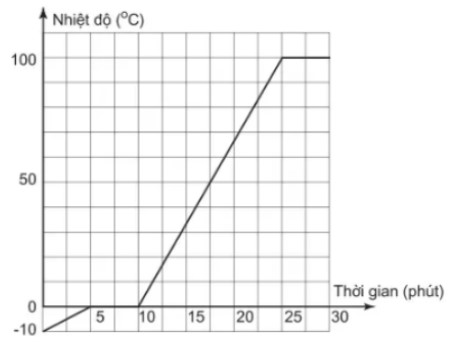
\includegraphics[width=0.45\linewidth]{figs/VN12-Y24-PH-SYL-001P-4}
\end{center}
\begin{enumerate}[label=\alph*)]
	\item Trong 5 phút đầu tiên, nước ở thể rắn.
	\item Từ phút thứ 5 đến phút thứ 10 nước đá nóng chảy.
	\item Từ phút thứ 10 đến phút thứ 25 nước không có sự bay hơi vì chưa đạt nhiệt độ sôi.
	\item Nước được đun ở điều kiện tiêu chuẩn.
\end{enumerate}
\loigiai{
	\begin{enumerate}[label=\alph*)]
		\item Đúng.
		\item Đúng.
		\item Sai. Nước bay hơi ở bất kì nhiệt độ nào.
		\item Đúng. Đồ thị thể hiện quá trình nước sôi ở $\SI{100}{\celsius}$.
	\end{enumerate}
}
\end{ex}

%=====================================================================================
\begin{ex}
	Bảng dưới đây ghi nhận nhiệt độ nóng chảy và nhiệt độ sôi của một số chất
	\begin{center}
		\begin{tabular}{|C{8em}|C{10em}|C{8em}|}
			\hline
			\thead{Chất}& \thead{Nhiệt độ nóng chảy} &\thead{Nhiệt độ sôi}\\
			\hline
			Chì & $\SI{327}{\celsius}$ & $\SI{1613}{\celsius}$\\
			\hline
			Nước & $\SI{0}{\celsius}$ & $\SI{100}{\celsius}$\\
			\hline
			Oxygen & $\SI{-219}{\celsius}$ & $\SI{-183}{\celsius}$\\
			\hline
			Rượu & $\SI{-117}{\celsius}$ & $\SI{78}{\celsius}$\\
			\hline
			Thuỷ ngân & $\SI{-39}{\celsius}$ & $\SI{357}{\celsius}$\\
			\hline
		\end{tabular}
	\end{center}
	\begin{enumerate}[label=\alph*)]
		\item Chì có nhiệt độ sôi cao nhất trong các chất được liệt kê.
		\item Nước có nhiệt độ sôi thấp nhất trong các chất được liệt kê.
		\item Ở nhiệt độ $\SI{30}{\celsius}$ thì chì ở thể  rắn.
		\item Ở nhiệt độ $\SI{30}{\celsius}$ thì oxide ở thể lỏng.
	\end{enumerate}
	\loigiai{
		\begin{enumerate}[label=\alph*)]
			\item Đúng.
			\item Sai.
			\item Đúng.
			\item Sai. 
		\end{enumerate}
	}
\end{ex}
%====================================================================================
\begin{ex}
	Hình bên là một cốc nước đá đặt ngoài không khí.
	\begin{center}
		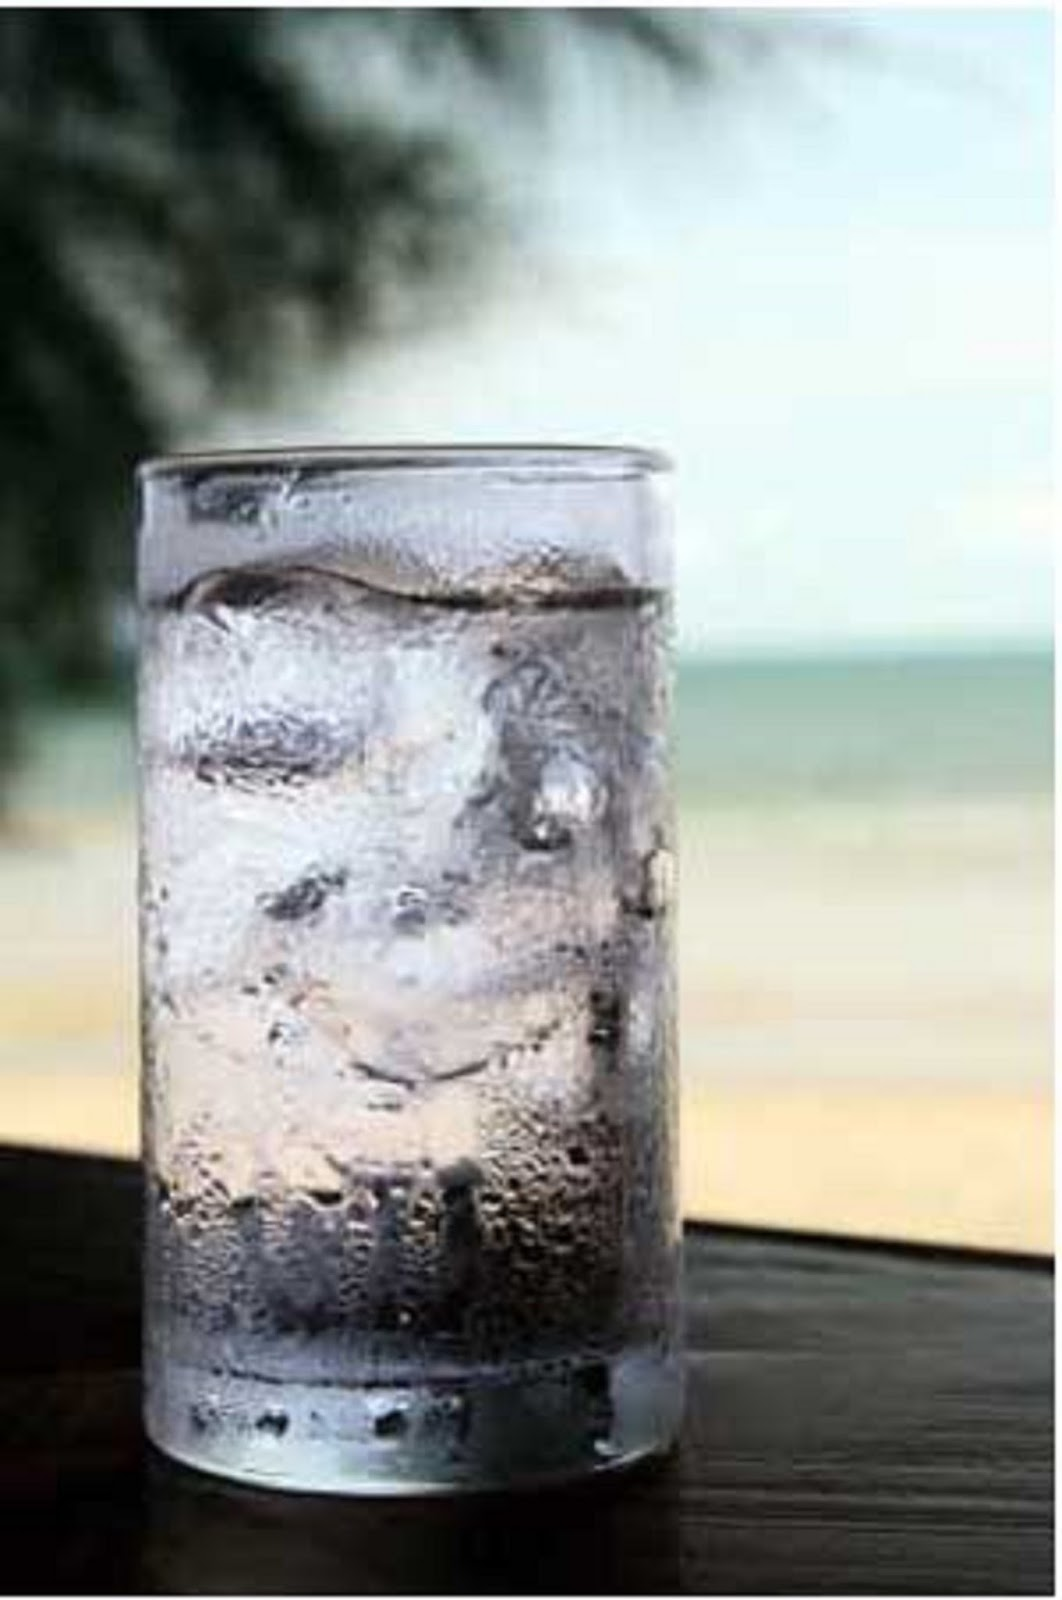
\includegraphics[width=0.2\linewidth]{figs/VN12-Y24-PH-SYL-001P-3}
	\end{center}

	\begin{enumerate}[label=\alph*)]
		\item 
		Nước ngưng đọng trên thành cốc là do nước bên trong cốc thấm ra ngoài.
		\item Nước đá truyền nhiệt ra bên ngoài làm đá tan dần.
		\item Khói trắng xuất hiện trên miệng cốc là do sự hoá hơi của nước trong cốc.
		\item Khi đá chưa tan hết thì nhiệt độ của nước trong cốc là $\SI{0}{\celsius}$.
	\end{enumerate}
	\loigiai{
		\begin{enumerate}[label=\alph*)]
			\item Sai. Nước đọng trên thành cốc là do hơi nước trong không khí gần cốc ngưng tụ.
			\item Sai. Nước đá nhận nhiệt từ môi trường nên tan dần.
			\item Sai. Khói trắng xuất hiện ở miệng cốc là kết quả sự ngưng tụ của hơi nước trong không khí.
			\item Đúng.
		\end{enumerate}
	}
	\end{ex}
\Closesolutionfile{ans}
\subsection{Bài tập tự luận}
\setcounter{ex}{0}
\begin{ex}
	Hãy sử dụng mô hình động học phân tử để giải thích vì sao chúng ta có thể đi trong không khí, bơi trong nước nhưng không thể đi xuyên qua tường?
	\loigiai{
		Lực liên kết giữa các phân tử chất rắn lớn hơn nhiều so với lực liên kết giữa các phân tử chất lỏng và chất khí. Do đó, ta khó bẽ gãy được liên kết của các phân tử chất rắn nên không thể đi xuyên qua tường.
		
	}
	\end{ex}
%=====================================================================================
\begin{ex}
Cùng một chất, khi ở thể lỏng thường có khối lượng riêng nhỏ hơn khi ở thể rắn và khối lượng riêng ở thế khí lại nhỏ hơn khi ở thể lỏng. Vì sao như vậy?
	\loigiai{Vì khoảng cách trung bình giữa các phân tử chất khí lớn hơn khoảng cách trung bình giữa các phân tử chất lỏng và lớn hơn khoảng cách trung bình giữa các phân tử chất rắn. Do đó, với cùng một chất thì thể khí thường có thể tích lớn hơn so với với thể lỏng và lớn hớn thể tích ở rắn. Vì vậy, ở thể lỏng thường có khối lượng riêng nhỏ hơn khi ở thể rắn và khối lượng riêng ở thế khí lại nhỏ hơn khi ở thể lỏng.}
\begin{note}
Không đúng cho tất cả trường hợp. Ví dụ, nước có thể tích ở thể rắn lớn hơn thể tích ở thể lỏng
\end{note}
	\end{ex}
%=====================================================================================
\begin{ex}
Cồn y tế chuyển từ thể lỏng sang thể khí rất nhanh ở điều kiện thông thường. Hãy giải thích tại sao khi xoa cồn vào da, ta cảm thấy lạnh ở vùng da đó?
	\loigiai{
		Khi cồn chuyển thể từ lỏng sang khí thì cần thu nhiệt lượng, do đó tay ta mất bớt nhiệt lượng truyền cho cồn và cảm thấy vùng da thoa cồn bị lạnh đi.
		
	}
	\end{ex}
%=====================================================================================
\begin{ex}
	Vì sao bình nước sôi muốn để nguội nhanh thì cần mở nắp để hơi nước thoát ra?
	\loigiai{
		Vì hơi nước có nhiệt độ cao, khi mở nắp thì hơi nước thoát ra nhiều và nhanh hơn làm cho nước còn lại trong bình dễ trao đổi nhiệt với không khí bên ngoài và giảm nhanh nhiệt độ.
	}
\end{ex}
%=====================================================================================
\begin{ex}
	Rau xanh sau khi mua về thường bị héo khi để ở ngoài trời nắng. Vì sao lại có hiện tượng trên? Làm thế nào để hạn chế điều này?
	\loigiai{
		Rau bị héo là do sự bay hơi của nước trong rau qua bề mặt lá. Để hạn chế rau nhanh héo có thể thực hiện các cách sau
		\begin{itemize}
			\item Tránh ánh nắng trực tiếp từ mặt trời, bảo quản ở nơi thoáng mát.
			\item Vẫy nước lên rau để tạo lớp nước bám trên bề mặt, lớp nước này sẽ hấp thụ nhiệt từ môi trường và bay hơi trước.
		\end{itemize}
		
	}
\end{ex}
%=====================================================================================
\begin{ex}
	Để khử trùng các dụng cụ y tế nhiều lần (kéo, kẹp gắp, dao mổ, \dots), ngày nay người ta thường sấy chúng trong lò sấy ở nhiệt độ cao. Tuy nhiên, trước đây người ta thường phải luộc chúng trong nước sôi. Giả sử cần phải thực hiện nhiệm vụ này nhưng có một số vi khuẩn chỉ bị tiêu diệt ở nhiệt độ $\SI{105}{\celsius}$, trong đó khi nhiệt độ sôi của nước ở điều kiện tiêu chuẩn là $\SI{100}{\celsius}$. Hãy đề xuất phương án đơn giản để diệt các vi khuẩn này và giải thích.
	\loigiai{
		Tăng áp suất đun nước (dùng nối áp suất) để tăng nhiệt độ sôi của nước.
	}
\end{ex}
%=====================================================================================
\begin{ex}
Một người thợ mộc sau khi đánh vecni vào một số chân giường, sau một thời gian, người thợ mộc phát hiện thấy những chân giường chưa được đánh vecni bị nứt (rạn chân chim), còn những chân giường đã được đánh vecni thì không bị như thế. Hãy giải thích tại sao?
	\loigiai{
		Trong gỗ có chứa một lượng nước nhất định, khi đánh vecni lên gỗ, lớp vecni ngăn cách sự tiếp xúc của gỗ với môi trường bên ngoài và làm hạn chế sự bay hơi của nước trong gỗ. Còn những chân giường không đánh vecni thì nước trong gỗ bị bay hơi và làm gỗ bị khô, nứt.
	}
\end{ex}
	
%\newpage\section{NHIỆT ĐỘ - THANG NHIỆT ĐỘ}
\subsection{LÝ THUYẾT TRỌNG TÂM}
\subsubsection{Chiều truyền năng lượng nhiệt giữa hai vật chênh lệch nhiệt độ tiếp xúc nhau}
\begin{boxdn}
	Khi cho hai vật chênh lệch nhiệt độ tiếp xúc nhau, năng lượng nhiệt luôn truyền từ vật có nhiệt độ cao hơn sang vật có nhiệt độ thấp hơn. Quá trình truyền nhiệt kết thúc khi hai vật ở cùng nhiệt độ (trạng thái cân bằng nhiệt).
\end{boxdn}
\begin{center}
	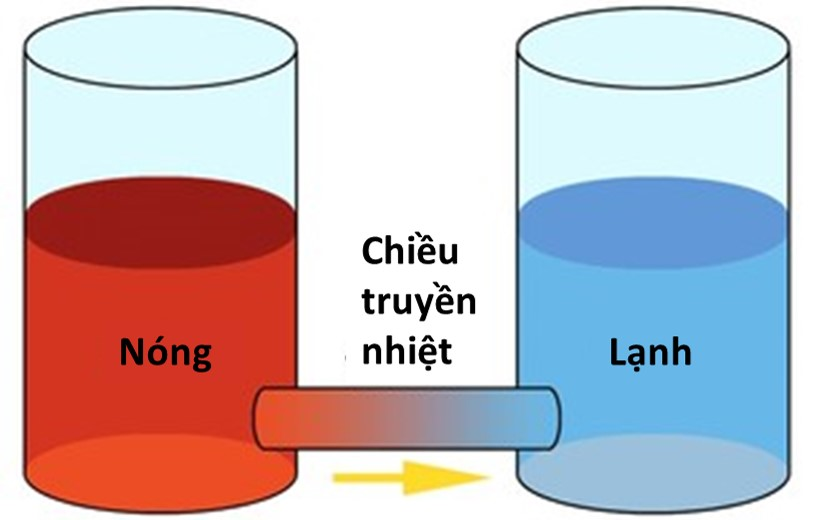
\includegraphics[width=0.3\linewidth]{figs/VN12-Y24-PH-SYL-002-1}
	\captionof{figure}{Minh hoạ chiều truyền nhiệt giữa hai vật có nhiệt độ khác nhau}
\end{center}
\subsubsection{Nhiệt độ}
\paragraph{Khái niệm về nhiệt độ}
\begin{boxdn}
	Nhiệt độ của một vật là đại lượng vật lí đặc trưng cho mức độ chuyển động nhiệt của phân tử vật chất cấu tạo nên vật. Khi các phân tử chuyển động nhiệt càng nhanh thì nhiệt độ của vật càng cao và ngược lại.
\end{boxdn}
\paragraph{Nhiệt kế}
\begin{boxdn}
	Nhiệt độ đo trên nhiệt kế được xác định thông qua giá trị của một đại lượng vật lí khác mà đại lượng này phụ thuộc theo nhiệt độ.
\end{boxdn}
\begin{boxvidu}
	\textbf{\textit{Ví dụ:}}
	\begin{itemize}
		\item Nhiệt kế thuỷ ngân xác định nhiệt độ dựa trên hiện tượng dãn nở vì nhiệt của thuỷ ngân.
		\item Nhiệt kế điện trở xác định nhiệt độ qua sự phụ thuộc của điện trở theo nhiệt độ.
	\end{itemize}
\end{boxvidu}
\begin{center}
	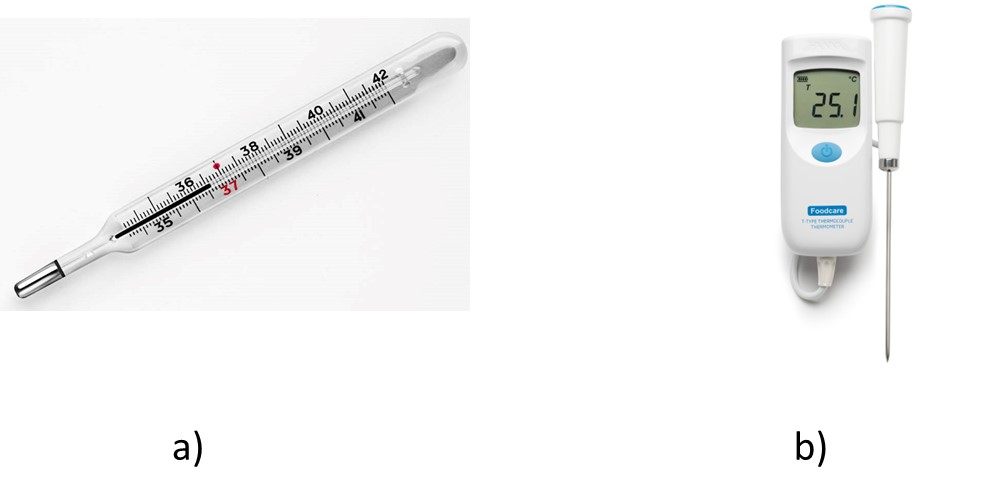
\includegraphics[width=0.5\linewidth]{figs/VN12-Y24-PH-SYL-002-2}
	\captionof{figure}{a) Nhiệt kế thuỷ ngân; b) Nhiệt kế điện trở}
\end{center}
\subsubsection{Thang nhiệt độ}
\paragraph{Thang nhiệt độ Celsius}
\begin{boxdn}
	Nhiệt độ trong thang đo này được kí hiệu là $t$. Đơn vị là độ Celsius (kí hiệu: $\si{\celsius}$).\\
	$\SI{1}{\celsius}=\dfrac{1}{100}$ của khoảng cách giữa nhiệt độ nóng chảy của nước tinh khiết đóng băng $\left(\SI{0}{\celsius}\right)$ và nhiệt độ sôi của nước tinh khiết ở áp suất $\SI{1}{atm}$ ($\SI{100}{\celsius}$).
\end{boxdn}

\paragraph{Thang nhiệt độ Kelvin}
\begin{boxdn}
	Nhiệt độ trong thang đo này được kí hiệu là $T$. Đơn vị là độ Kelvin (kí hiệu: $\si{\kelvin}$).\\
	$\SI{1}{\kelvin}=\dfrac{1}{273,15}$ của khoảng cách giữa nhiệt độ không tuyệt đối $\left(\SI{0}{\kelvin}\right)$ và nhiệt độ điểm mà nước tinh khiết tồn tại đồng thời ở thể rắn, lỏng và hơi ở áp suất $\SI{1}{atm}$ ($\SI{273.15}{\kelvin}$).\\
	Nhiệt độ không tuyệt đối ($\SI{0}{\kelvin}$) là nhiệt độ mà tại đó động năng chuyển động nhiệt của các phân tử cấu tạo nên vật chất bằng không và thế năng của chúng là tối thiểu.
\end{boxdn}
\begin{luuy}
	Một độ chia trên thang nhiệt độ Kelvin bằng một độ chia trên thang nhiệt độ Celsius.
\end{luuy}
\paragraph{Chuyển đổi nhiệt độ đo theo thang Celsius sang nhiệt độ đo theo thang Kelvin}
\begin{boxdl}
	\begin{equation}
		T=t+273,15\approx t+273
	\end{equation}
\end{boxdl}
với:
\begin{itemize}
	\item $t$: giá trị nhiệt độ của vật theo thang nhiệt độ Celsius;
	\item $T$: giá trị nhiệt độ của vật theo thang nhiệt độ Kelvin.
\end{itemize}
\subsection{VÍ DỤ MINH HOẠ}
\begin{dang}{Chuyển đổi được nhiệt độ đo theo thang Celsius sang nhiệt độ đo theo thang Kelvin và ngược lại}

\end{dang}
	\begin{vd}
Nhiệt độ của khối khí trong phòng đo được là $\SI{27}{\celsius}$. Xác định nhiệt độ của khối khí trong thang nhiệt độ Kelvin.
		\loigiai{
			Nhiệt độ khối khí trong thang nhiệt độ Kelvin:
			$$T=t+273=\SI{300}{\kelvin}.$$}
		
	
\end{vd}

\begin{vd}
	Một nhiệt kế dùng để đo nhiệt độ của các lò nung có phạm vi đo từ $\SI{263}{\kelvin}$ đến $\SI{1273}{\kelvin}$.
	\begin{enumerate}[label=\alph*)]
		\item Xác định phạm vi đo của nhiệt kế này trong thang nhiệt độ Celsius?
		\item Nếu sử dụng nhiệt kế này để đo nhiệt độ lò nung đang nấu chảy đồng có nhiệt độ nóng chảy là $\SI{1083}{\celsius}$ thì nhiệt kế có đo được không? Vì sao? Em có khuyến cáo gì về việc sử dụng nhiệt kế trong tình huống này?
	\end{enumerate}
	\loigiai{
		\begin{enumerate}[label=\alph*)]
			\item $t_\text{min}=T_\text{min}-273=\SI{-10}{\celsius};\quad t_\text{max}=T_\text{max}-273=\SI{1000}{\celsius}.$\\
			Phạm vi đo của nhiệt kế này trong thang nhiệt độ Celsius là $\SI{-10}{\celsius}$ đến $\SI{1000}{\celsius}$.
			\item Nếu sử dụng nhiệt kế này để đo nhiệt độ lò nung đang nấu chảy đồng có nhiệt độ nóng chảy $\SI{1083}{\celsius}$ thì nhiệt kế không đo được vì nhiệt độ cần đo nằm khoảng phạm vi đo của nhiệt kế.\\
			Trong trường hợp này, người đo cần dùng nhiệt kế có thang đo lớn hơn $\SI{1083}{\celsius}$ như nhiệt kế điện trở.
	\end{enumerate}}
\end{vd}

\begin{vd}
	Trong thang nhiệt độ Fahrenheit, chọn nhiệt độ tại điểm nước đá đang tan là $\SI{32}{\degree F}$, nhiệt độ tại điểm nước sôi ở điều kiện thường $\left(\SI{1}{atm}\right)$ là $\SI{212}{\degree F}$, trong khoảng nhiệt độ này chia thành 180 khoảng bằng nhau, mỗi khoảng ứng với $\SI{1}{\degree F}$. Thang đo này được nhà vật lí người Đức Daniel Gabriel Fahrenheit đề xuất vào năm 1724 và được sử dụng phổ biến ở các nước phương Tây. Nếu gọi $t$ là nhiệt độ của vật trong thang nhiệt độ Celsius và $T_\text{F}$ nhiệt độ của vật trong thang nhiệt độ Fahrenheit thì:
	$$T_\text{F}=a\cdot t+b.$$
	với $a$ và $b$ là các hệ số tỉ lệ.
	\begin{enumerate}[label=\alph*)]
		\item Em hãy xác định xác giá trị của $a$ và $b$.
		\item Trên tin tức thông báo nhiệt độ tại New York ngày 17/03/2024 là $\SI{49}{\degree F}$. Trong thang Celsius thì nhiệt độ này là bao nhiêu $\si{\celsius}$?
	\end{enumerate}
	\loigiai{
		\begin{enumerate}[label=\alph*)]
			\item Nhiệt độ tại điểm nước đá đang tan là $\SI{32}{\degree F}$ hay $\SI{0}{\celsius}$:
			\begin{equation}
				\label{eq: 1}\\
				b=\SI{32}{\degree F}
			\end{equation}
			Nhiệt độ tại điểm nước sôi ở điều kiện thường $\left(\SI{1}{atm}\right)$ là $\SI{212}{\degree F}$ hay $\SI{100}{\celsius}$:
			\begin{equation}
				\label{eq: 2}\\
				212=100a+b
			\end{equation}
			Từ (\ref{eq: 1}) và (\ref{eq: 2}), suy ra:
			\begin{equation*}
				\begin{cases}
					b=\SI{32}{\degree F}\\
					a=\SI{1.8}{\degree F/\celsius}
				\end{cases}
			\end{equation*}
			Như vậy, $T_\text{F}=1,8\cdot t+32.$
			\item Nhiệt độ tại New York ngày 17/03/2024 theo thang Celsius:
			$$t=\dfrac{T_\text{F}-32}{1,8}\approx\SI{9.44}{\celsius}.$$
	\end{enumerate}}
\end{vd}
\begin{luuy}
	$$\dfrac{t\left(\si{\degree F}\right)-32}{212-32}=\dfrac{t\left(\si{\celsius}\right)-0}{100-0}=\dfrac{T\left(\si{\kelvin}\right)-273}{373-273}.$$
\end{luuy}
\subsection{BÀI TẬP TRẮC NGHIỆM}
\inputansbox{10}{ans/G12Y24B2TN}
\Opensolutionfile{ans}[ans/G12Y24B2TN]
\begin{ex}
	Cho hai vật có nhiệt độ khác nhau tiếp xúc với nhau. Nhiệt được truyền từ
	\choice
	{vật có khối lượng lớn hơn sang vật có khối lượng nhỏ hơn}
	{\True vật có nhiệt độ cao hơn sang vật có nhiệt độ thấp hơn}
	{vật ở trên cao sang vật ở dưới thấp}
	{vật có khối lượng riêng lớn sang vật có khối lượng riêng nhỏ}
	\loigiai{

}
	\end{ex}
%====================================================================================
\begin{ex}
Người ta cho hai vật dẫn nhiệt A và B tiếp xúc với nhau, sau một thời gian khi có trạng thái cân bằng nhiệt thì hai vật này có
	\choice
	{\True cùng nhiệt độ}
	{cùng nội năng}
	{cùng năng lượng}
	{cùng nhiệt lượng}
	\loigiai{
	
}
\end{ex}

%====================================================================================
\begin{ex}
Đơn vị đo nhiệt độ trong thang nhiệt Celsius là
	\choice
	{$\si{\kelvin}$}
	{$\si{\degree F}$}
	{$\si{\newton}$}
	{\True $\si{\celsius}$}
	\loigiai{
		
	}
\end{ex}
%====================================================================================
\begin{ex}
	Nhiệt kế chất lỏng được chế tạo dựa trên nguyên tắc nào?
	\choice
	{\True Sự nở vì nhiệt của chất lỏng}
	{Sự phụ thuộc của tốc độ dòng chảy theo nhiệt độ}
	{Sự thay đổi điện trở của khối chất lỏng theo nhiệt độ}
	{Sự phụ thuộc của áp suất chất lỏng theo nhiệt độ}
	\loigiai{
		
	}
\end{ex}
%====================================================================================
\begin{ex}
Trong các nhiệt kế sau đây, em hãy chọn nhiệt kế phù hợp để đo nhiệt độ của nước đang được đun sôi?
	\choice
	{Nhiệt kế y tế có thang chia độ từ $\SI{35}{\celsius}$ đến $\SI{42}{\celsius}$}
	{ Nhiệt kế rượu có thang chia độ từ $\SI{-30}{\celsius}$ đến $\SI{60}{\celsius}$}
	{\True Nhiệt kế thuỷ ngân có thang chia độ từ $\SI{-10}{\celsius}$ đến $\SI{110}{\celsius}$}
	{Nhiệt kế hồng ngoại có thang chia độ từ $\SI{30}{\celsius}$ đến $\SI{45}{\celsius}$}
	\loigiai{
		
	}
\end{ex}
%====================================================================================
\begin{ex}
	Cách xác định nhiệt độ trong thang nhiệt độ Celsius là
	\choice
	{Lấy nhiệt độ của nước khi đóng băng là $\left(\SI{10}{\celsius}\right)$ và nhiệt độ sôi của nước $\left(\SI{100}{\celsius}\right)$ làm chuẩn}
	{Lấy nhiệt độ của nước khi đóng băng là $\left(\SI{100}{\celsius}\right)$ và nhiệt độ sôi của nước $\left(\SI{0}{\celsius}\right)$ làm chuẩn}
	{\True Lấy nhiệt độ của nước khi đóng băng là $\left(\SI{0}{\celsius}\right)$ và nhiệt độ sôi của nước $\left(\SI{100}{\celsius}\right)$ làm chuẩn}
	{Lấy nhiệt độ của nước khi đóng băng là $\left(\SI{100}{\celsius}\right)$ và nhiệt độ sôi của nước $\left(\SI{10}{\celsius}\right)$ làm chuẩn}
	\loigiai{
		
	}
\end{ex}
%====================================================================================
\begin{ex}
	Điểm đóng băng và sôi của nước theo thang Kelvin là
	\choice
	{$\SI{0}{\kelvin}$ và $\SI{100}{\kelvin}$}
	{\True $\SI{273}{\kelvin}$ và $\SI{373}{\kelvin}$}
	{$\SI{37}{\kelvin}$ và $\SI{73}{\kelvin}$}
	{$\SI{32}{\kelvin}$ và $\SI{212}{\kelvin}$}
	\loigiai{
		
	}
\end{ex}

%====================================================================================
\begin{ex}
	Độ không tuyệt đối là nhiệt độ ứng với
	\choice
	{\True $\SI{0}{\kelvin}$}
	{$\SI{0}{\celsius}$}
	{$\SI{273}{\kelvin}$}
	{$\SI{273}{\celsius}$}
	\loigiai{
		
	}
\end{ex}
%====================================================================================
\begin{ex}
	Chọn phát biểu \textbf{đúng}.\\
	Nhiệt độ không tuyệt đối là nhiệt độ mà tại đó
	\choice
	{\True chuyển động nhiệt của phân tử hầu như dừng lại}
	{nước bắt đầu đông thành đá}
	{tất cả chất khí hoá lỏng}
	{tất cả chất khí hoá rắn}
	\loigiai{
		
	}
\end{ex}
%====================================================================================
\begin{ex}
Không thể dùng nhiệt kế rượu để đo nhiệt độ của nước đang sôi vì
	\choice
	{rượu sôi ở nhiệt độ cao hơn $\SI{100}{\celsius}$}
	{\True rượu sôi ở nhiệt độ thấp hơn $\SI{100}{\celsius}$}
	{rượu đông đặc ở nhiệt độ $\SI{100}{\celsius}$}
	{rượu đông đặc ở nhiệt độ thấp hơn $\SI{0}{\celsius}$}
	\loigiai{
		
	}
\end{ex}
%====================================================================================
\begin{ex}
Biểu thức nào sau đây là đúng khi biến đổi nhiệt độ từ thang Celsius sang thang Kelvin?
	\choice
	{$T\left(\si{\kelvin}\right)=t\left(\si{\celsius}\right)-273$}
	{\True $T\left(\si{\kelvin}\right)=t\left(\si{\celsius}\right)+273$}
	{$T\left(\si{\kelvin}\right)=\dfrac{t\left(\si{\celsius}\right)+273}{2}$}
	{$T\left(\si{\kelvin}\right)=2t\left(\si{\celsius}\right)+273$}
	\loigiai{
		
	}
\end{ex}
%====================================================================================
\begin{ex}
Cho các bước như sau:
\begin{enumerate}[label=(\arabic*)]
	\item Thực hiện phép đo nhiệt độ.
	\item Ước lượng nhiệt độ của vật.
	\item Hiệu chỉnh nhiệt kế.
	\item Lựa chọn nhiệt kế phù hợp.
	\item Đọc và ghi kết quả đo.
\end{enumerate}
Các bước đúng khi thực hiện đo nhiệt độ của một vật là
	\choice
	{\True (2), (4), (3), (1), (5)}
	{(1), (4), (2), (3), (5)}
	{(1), (2), (3), (4), (5)}
	{(3), (2), (4), (1), (5)}
	\loigiai{
		
	}
\end{ex}
%====================================================================================
\begin{ex}
Nhiệt độ trung bình của nước ở thang nhiệt độ Celsius là $\SI{27}{\celsius}$ ứng với thang nhiệt độ Kelvin thì nhiệt độ của nước là
	\choice
	{$\SI{273}{\kelvin}$}
	{\True $\SI{300}{\kelvin}$}
	{$\SI{246}{\kelvin}$}
	{$\SI{327}{\kelvin}$}
	\loigiai{
			$$T=t+273=\SI{300}{\kelvin}.$$
	}
\end{ex}
%====================================================================================
\begin{ex}
Nhiệt độ mùa đông tại thành phố New York (Mỹ) là $\SI{283}{\kelvin}$, ứng với nhiệt giai Celsius thì nhiệt độ ở đó là
	\choice
	{\True $\SI{10}{\celsius}$}
	{$\SI{-10}{\celsius}$}
	{$\SI{5}{\celsius}$}
	{$\SI{-5}{\celsius}$}
	\loigiai{
		$$t=T-273=\SI{10}{\celsius}.$$
	}
\end{ex}


%====================================================================================
\begin{ex}
	Nhiệt độ vào một ngày mùa hè ở thành phố Hồ Chí Minh là $\SI{35}{\celsius}$. Nhiệt độ đó tương ứng với bao nhiêu độ $\si{\degree F}$?
	\choice
	{$\SI{59}{\degree F}$}
	{$\SI{67}{\degree F}$}
	{\True $\SI{95}{\degree F}$}
	{$\SI{76}{\degree F}$}
	\loigiai{
		$$t\left(\si{\degree F}\right)=32+1,8t\left(\si{\celsius}\right)=\SI{95}{\degree F}.$$
	}
\end{ex}
%====================================================================================
\begin{ex}
	Giá trị nhiệt độ đo được theo thang nhiệt độ Kelvin là $\SI{293}{\kelvin}$. Tính theo thang nhiệt độ Fahrenheit, nhiệt độ đó có giá trị là
	\choice
	{$\SI{20}{\degree F}$}
	{$\SI{100}{\degree F}$}
	{\True $\SI{68}{\degree F}$}
	{$\SI{261}{\degree F}$}
	\loigiai{
		$$t\left(\si{\celsius}\right)=T-273=\SI{20}{\celsius}.$$
	$$t\left(\si{\degree F}\right)=32+1,8t\left(\si{\celsius}\right)=\SI{68}{\degree F}.$$}
\end{ex}
%====================================================================================
\begin{ex}
	$\SI{104}{\degree F}$ ứng với bao nhiêu độ Kelvin?
	\choice
	{\True $\SI{313}{\kelvin}$}
	{$\SI{298}{\kelvin}$}
	{$\SI{328}{\kelvin}$}
	{$\SI{293}{\kelvin}$}
	\loigiai{
		$$\dfrac{t\left(\si{\degree F}\right)-32}{212-32}=\dfrac{T\left(\si{\kelvin}\right)-273}{373-273}$$
		Thay $t\left(\si{\degree F}\right)=\SI{104}{\degree F}$, thu được $T=\SI{313}{\kelvin}.$}
	\end{ex}
%====================================================================================
\begin{ex}
	Một thang đo $X$ lấy điểm đóng băng là $-10X$, lấy điểm sôi là $90X$. Nhiệt độ của một vật đọc được trên theo nhiệt giai Celsius là $\SI{40}{\celsius}$ thì trong nhiệt giai $X$ có nhiệt độ bằng
	\choice
	{$20X$}
	{\True $30X$}
	{$40X$}
	{$50X$}
	\loigiai{
		Độ chênh lệch nhiệt độ tại điểm băng và điểm sôi trong thang X cũng là 100. Như vậy $\SI{1}{\celsius}$ tương ứng với $\SI{1}{X}$ và
		$$t\left(\si{\celsius}\right)=t\left(\si{X}\right)+10.$$
	}
\end{ex}
%====================================================================================
\begin{ex}
	Giả sử có một thang nhiệt độ kí hiệu Z. Nhiệt độ sôi của nước theo thang này là $60Z$, điểm ba cả nước là $-15Z$. Nhiệt độ của vật theo thang Fahrenheit là bao nhiêu nếu nhiệt độ trong thang Z là $-96Z$?Giả sử có một thang nhiệt độ kí hiệu Z. Nhiệt độ sôi của nước theo thang này là $60Z$, điểm ba cả nước là $-15Z$. Nhiệt độ của vật theo thang Fahrenheit là bao nhiêu nếu nhiệt độ trong thang Z là $-96Z$?
	\choice
	{$\SI{-62.4}{\degree F}$}
	{$\SI{162.4}{\degree F}$}
	{\True $\SI{-162.4}{\degree F}$}
	{$\SI{62.4}{\degree F}$}
	\loigiai{
	$$\dfrac{t\left(\si{\degree F}\right)-32}{212-32}=\dfrac{Z-\left(-15\right)}{60-\left(-15\right)}$$
	Thay $Z=-96$ ta thu được $t\left(\si{\degree F}\right)=\SI{-162.4}{\degree F}.$
	}
\end{ex}
%====================================================================================
\begin{ex}
Hình dưới thể hiện nhiệt kế đo nhiệt độ của một vật. Sai số dụng cụ được lấy bằng một nửa độ chia nhỏ nhất. Kết quả đo nhiệt độ của vật này là
\begin{center}
	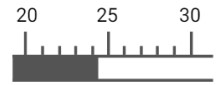
\includegraphics[width=0.25\linewidth]{figs/VN12-Y24-PH-SYL-002P-3}
\end{center}
	\choice
	{\True $t=\xsi{24.0\pm0.5}{\celsius}$}
	{$t=\xsi{25.0\pm0.5}{\celsius}$}
	{$t=\xsi{24.0\pm1.0}{\celsius}$}
	{$t=\xsi{25.0\pm1.0}{\celsius}$}
	\loigiai{
		
	}
\end{ex}

%====================================================================================
\begin{ex}
Chiều dài của phần thuỷ ngân trong nhiệt kế là $\SI{2}{\centi\meter}$ ở $\SI{0}{\celsius}$ và $\SI{22}{\centi\meter}$ ở $\SI{100}{\celsius}$. Nhiệt độ là bao nhiêu nếu chiều dài của thuỷ ngân là $\SI{8}{\centi\meter}$?
	\choice
	{$\SI{40}{\celsius}$.$\SI{40}{\celsius}$}
	{$\SI{50}{\celsius}$}
	{$\SI{20}{\celsius}$}
	{\True $\SI{30}{\celsius}$}
	\loigiai{
		$$\dfrac{\ell-\ell_0}{t-t_0}=\dfrac{\ell'-\ell_0}{t'-t_0}$$
		$$\Leftrightarrow\dfrac{\SI{22}{\centi\meter}-\SI{2}{\centi\meter}}{\SI{100}{\celsius}-\SI{0}{\celsius}}=\dfrac{\SI{8}{\centi\meter}-\SI{2}{\centi\meter}}{t'-\SI{0}{\celsius}}\Rightarrow t'=\SI{30}{\celsius}.$$
	}
\end{ex}
%====================================================================================
\begin{ex}
Chiều dài của phần thuỷ ngân trong nhiệt kế là $\SI{2}{\centi\meter}$ ở $\SI{0}{\celsius}$ và $\SI{22}{\centi\meter}$ ở $\SI{100}{\celsius}$. Chiều dài của phần thuỷ ngân sẽ là bao nhiêu nếu nhiệt độ là $\SI{50}{\celsius}$?
	\choice
	{$\SI{10}{\centi\meter}$}
	{\True $\SI{12}{\centi\meter}$}
	{$\SI{14}{\centi\meter}$}
	{$\SI{16}{\centi\meter}$}
	\loigiai{
	$$\dfrac{\ell-\ell_0}{t-t_0}=\dfrac{\ell'-\ell_0}{t'-t_0}$$
	$$\Leftrightarrow\dfrac{\SI{22}{\centi\meter}-\SI{2}{\centi\meter}}{\SI{100}{\celsius}-\SI{0}{\celsius}}=\dfrac{\ell'-\SI{2}{\centi\meter}}{\SI{50}{\celsius}-\SI{0}{\celsius}}\Rightarrow \ell'=\SI{12}{\centi\meter}.$$
	}
\end{ex}
%====================================================================================
\begin{ex}
Sự phụ thuộc vào nhiệt độ của bước sóng điện từ theo hệ thức Wien: $T\cdot\lambda_\text{max}=\SI{2900}{\left(\micro\meter\cdot\kelvin\right)}$ được dùng vào việc chế tạo các nhiệt kế thường dùng hằng ngày như
nhiệt kế hồng ngoại, cũng như các nhiệt kế trong thiên văn để đo nhiệt độ bề mặt của
các thiên thể. Xét một nhiệt kế hồng ngoại khi đo nhiệt độ cơ thể người như hình vẽ.
Bước sóng hồng ngoại do cơ thể người phát ra bằng xấp xỉ bằng
\begin{center}
	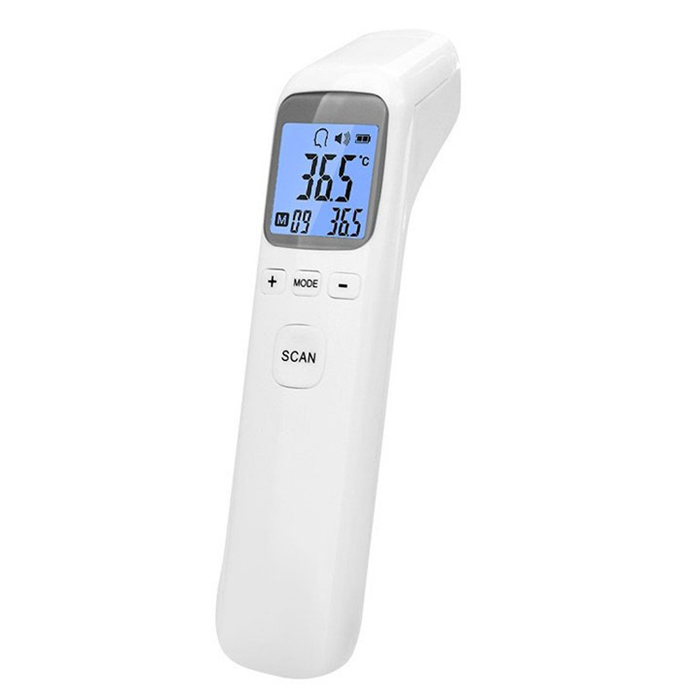
\includegraphics[width=0.3\linewidth]{figs/VN12-Y24-PH-SYL-002P-1}
\end{center}
	\choice
	{\True $\SI{9.4}{\micro\meter}$}
	{$\SI{79}{\micro\meter}$}
	{$\SI{29}{\micro\meter}$}
	{$\SI{10.6}{\micro\meter}$}
	\loigiai{
	$$\lambda_\text{max}=\dfrac{\SI{2900}{\micro\meter\cdot\kelvin}}{T}=\dfrac{\SI{2900}{\micro\meter\cdot\kelvin}}{36,5+\SI{273}{\kelvin}}\approx\SI{9.4}{\micro\meter}.$$
	}
\end{ex}
\Closesolutionfile{ans}
\subsection{TRẮC NGHIỆM ĐÚNG/SAI}
\setcounter{ex}{0}

\begin{ex}
		Bảng sau đây ghi sự thay đổi nhiệt độ của không khí theo thời gian dựa trên số liệu của một trạm khí tượng ở Hà Nội ghi được vào một ngày mùa đông.
	\begin{center}
		\begin{tabular}{|C{8em}|C{1.5em}|C{1.5em}|C{1.5em}|C{1.5em}|C{1.5em}|C{1.5em}|C{1.5em}|C{1.5em}|}
			\hline
			\thead{Thời gian (giờ)}& 1 & 4 & 7 & 10 & 13 & 16 & 19 & 22\\
			\hline
			\thead{Nhiệt độ $\left(\si{\celsius}\right)$} & 13 & 13 &13 & 18& 18 & 20 & 17 & 12\\
			\hline
		\end{tabular}
	\end{center}
	\begin{enumerate}[label=\alph*)]
		\item Nhiệt độ lúc 4 giờ là $\SI{286}{\kelvin}$.
		\item Nhiệt độ thấp nhất trong ngày là vào lúc 1 giờ.
		\item Nhiệt độ cao nhất trong ngày là vào lúc 16 giờ.
		\item Độ chênh lệch nhiệt độ trong ngày là $\SI{6}{\celsius}$.
	\end{enumerate}
	\loigiai{
	\begin{enumerate}[label=\alph*)]
		\item Đúng.
		\item Sai. Nhiệt độ thấp nhất là $\SI{12}{\celsius}$ vào lúc $\SI{22}{\hour}$.
		\item Đúng.
		\item Sai. Độ chênh lệch nhiệt độ trong ngày là $\SI{8}{\celsius}$.
	\end{enumerate}
	
}
	\end{ex}

% =================================================================================
\begin{ex}
	Bảng dưới đây ghi tên các loại nhiệt kế và thang đo của chúng
	\begin{center}
		\begin{tabular}{|C{5cm}|C{6cm}|}
			\hline
			\thead{Loại nhiệt kế} & \thead{Thang nhiệt độ}\\
			\hline
			Thuỷ ngân & Từ $\SI{-10}{\celsius}$ đến $\SI{110}{\celsius}$\\
			\hline
			Rượu & Từ $\SI{-30}{\celsius}$ đến $\SI{60}{\celsius}$\\
			\hline
			Kim loại & Từ $\SI{0}{\celsius}$ đến $\SI{400}{\celsius}$\\
			\hline
			Điện tử & Từ $\SI{34}{\celsius}$ đến $\SI{42}{\celsius}$\\
			\hline
		\end{tabular}
	\end{center}
	\begin{enumerate}[label=\alph*)]
		\item Dùng nhiệt kế kim loại để đo nhiệt độ nước sôi.
		\item Dùng nhiệt kế điện tử để đo nhiệt độ cơ thể người.
		\item Dùng nhiệt kế thuỷ ngân để đo nhiệt độ không khí trong phòng.
		\item Dùng nhiệt kế rượu để đo nhiệt độ bề mặt bàn là.
	\end{enumerate}
	\loigiai{
	\begin{enumerate}[label=\alph*)]
		\item Đúng.
		\item Đúng.
		\item Đúng.
		\item Sai.
	\end{enumerate}
}
	\end{ex}
% ================================================================================
	\begin{ex}
		Hình bên là một nhiệt kế rượu.
		\begin{center}
			
\includegraphics[width=0.25\linewidth]{figs/VN12-Y24-PH-SYL-002P-2}
		\end{center}
		\begin{enumerate}[label=\alph*)]
			\item Giới hạn đo của nhiệt kế là $\SI{120}{\celsius}$.
			\item Độ chia nhỏ nhất của nhiệt kế là $\SI{5}{\celsius}$.
			\item Nhiệt độ hiện tại trên nhiệt kế là $\SI{19}{\celsius}$.
			\item Có thể dùng nhiệt kế để xác định nhiệt độ của nước sôi.
		\end{enumerate}
		\loigiai{
		\begin{enumerate}[label=\alph*)]
			\item Sai. Giới hạn đo của nhiệt kế là $\SI{50}{\celsius}$.
			\item Đúng.
			\item Sai. ĐCNN của nhiệt kế là $\SI{5}{\celsius}$ nên không thể đọc được giá trị $\SI{19}{\celsius}$, nhiệt độ hiện tại có thể đọc từ nhiệt kế là $\SI{20}{\celsius}$.
			\item Sai. Giới hạn đo của nhiệt kế nhỏ hơn nhiệt độ nước sôi.
		\end{enumerate}
	}

		\end{ex}
\subsection{BÀI TẬP TỰ LUẬN}
\setcounter{ex}{0}
\begin{ex}
	Theo dự báo thời tiết ngày 17/04/2024 thì nhiệt độ trung bình ngày - đêm trong
	ngày hôm đó tại Thành phố Hồ Chí Minh là  $\SI{35}{\celsius}-\SI{25}{\celsius}$. Sự chênh lệch nhiệt độ này trong thang đo Kelvin là bao nhiêu $\si{\kelvin}$?
	\loigiai{
		$$\Delta T=\SI{10}{\kelvin}.$$	
}
	\end{ex}

% ===================================================================================
\begin{ex}
	Thế giới từng ghi nhận sự thay đổi nhiệt độ rất lớn diễn ra ở Spearfish, South Dakota vào ngày 22/01/1943. Lúc 7h30 sáng, nhiệt độ ngoài trời là $\SI{-20}{\celsius}$. Hai phút sau, nhiệt độ ngoài trời tăng lên đến $\SI{7.2}{\celsius}$. Xác định độ tăng nhiệt độ trung bình trong 2 phút đó theo đơn vị Kelvin/giây.
	\loigiai{
		$$\dfrac{\Delta T}{t}=\dfrac{\SI{27.2}{\kelvin}}{\SI{120}{\second}}\approx\SI{0.23}{\kelvin/\second}.$$
	}
	\end{ex}
% ===================================================================================
\begin{ex}
Ở $\SI{20}{\celsius}$ một thanh nhôm dài $\SI{12}{\meter}$. Tính nhiệt độ cần thiết để chiều dài thanh nhôm là $\SI{12.01}{\meter}$. Biết rằng khi nhiệt độ tăng thêm $\SI{1}{\celsius}$ thì thanh nhôm dài thêm $\SI{2.3E-5}{}$ chiều dài ban đầu.
\loigiai{
	$$\Delta\ell=\alpha\ell_0\Delta t$$
	với $\alpha=\SI{2.3E-5}{\kelvin^{-1}}$.
	$$\Rightarrow \Delta t=\dfrac{\Delta \ell}{\alpha\ell_0}=\SI{36.23}{\celsius}.$$
	Vậy nhiệt độ cần thiết để thanh nhôm dài $\SI{12.01}{\meter}$ là $\SI{56.23}{\celsius}$.
}
\end{ex}


% ===================================================================================
\begin{ex}
Một nhiệt kế thể tích không đổi hiển thị nhiệt độ $\SI{0}{\celsius}$ và $\SI{100}{\celsius}$ với các áp suất $\SI{60}{\centi\meter Hg}$ và $\SI{120}{\centi\meter Hg}$. Biết nhiệt độ đọc được là hàm bậc nhất của áp suất. Khi áp suất thuỷ ngân là $\SI{90}{\centi\meter Hg}$ thì nhiệt độ đọc được bằng bao nhiêu?
\loigiai{
	Ta có:
	$$t=a\cdot p+b\Rightarrow \dfrac{t-t_1}{t_2-t_1}=\dfrac{p-p_1}{p_2-p_1}.$$
	Thay $p=\SI{90}{\centi\meter Hg}$; $t_1=\SI{0}{\celsius}$; $t_2=\SI{100}{\celsius}$; $p_1=\SI{60}{\centi\meter Hg}$; $p_2=\SI{120}{\centi\meter Hg}$, ta thu được: $t=\SI{50}{\celsius}.$
}

\end{ex}



	
%\newpage\section{NỘI NĂNG - ĐỊNH LUẬT I NHIỆT ĐỘNG LỰC HỌC}
\subsection{LÝ THUYẾT TRỌNG TÂM}
\subsubsection{Nội năng}
\paragraph{Khái niệm nội năng}
\begin{boxdn}
	Nội năng của một vật là tổng động năng và thế năng tương tác của các phân tử cấu tạo nên vật. Nội năng của vật phụ thuộc vào nhiệt độ $T$ và thể tích $V$ của vật:
	$$U=f\left(T, V\right).$$
\end{boxdn}
Đơn vị của nội năng trong hệ SI là joule $\left(\si{\joule}\right)$.
\paragraph{Mối liên hệ giữa nội năng và năng lượng của các phân tử cấu tạo nên vật}
Khi năng lượng của các phân tử cấu tạo nên vật tăng thì nội năng của vật tăng và ngược lại.
\subsubsection{Các cách làm thay đổi nội năng}
\paragraph{Thực hiện công}
\begin{boxdn}
	Quá trình thực hiện công làm cho nội năng của hệ thay đổi, hệ nhận công thì nội năng của hệ tăng, hệ thực hiện công cho vật khác thì nội năng giảm.
\end{boxdn}
\begin{boxvidu}
	\textbf{\textit{Ví dụ 1:}} Dùng tay ấn mạnh và nhanh piston của một cylanh chứa khí, thể tích khí trong cylanh giảm xuống (thế năng tương tác giữa các phân tử khí tăng), đồng thời khí nóng lên (động năng chuyển động nhiệt của các phân tử khí tăng). Do đó, nội năng của khí tăng.
\end{boxvidu}
\begin{boxvidu}
	\textbf{\textit{Ví dụ 2:}} Chà xát hai thanh gỗ với nhau, bề mặt tiếp xúc của hai thanh gỗ nóng dần lên. Nội năng của thanh gỗ tăng.
\end{boxvidu}
\begin{center}
	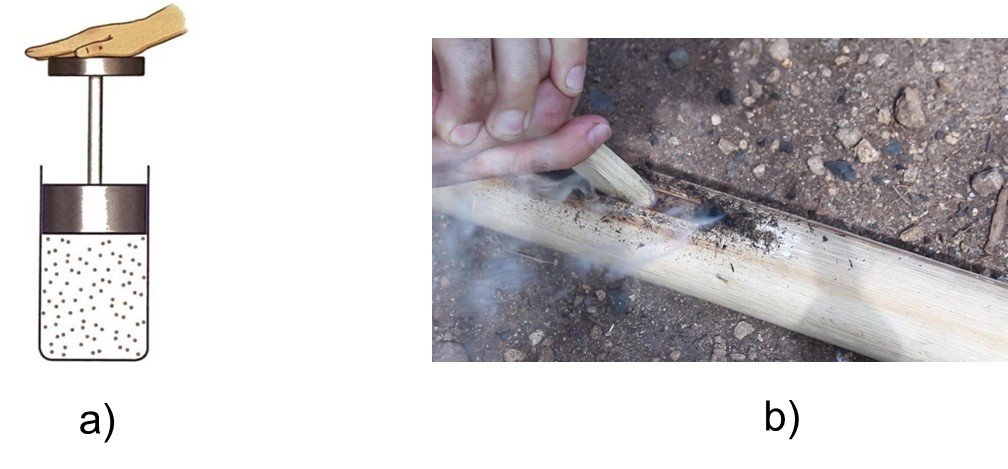
\includegraphics[width=0.45\linewidth	]{figs/VN12-Y24-PH-SYL-003-1}
	\captionof{figure}{a) Nén khối khí trong cylanh; b) Chà xát hai thanh gỗ với nhau}
\end{center}
\paragraph{Truyền nhiệt}
\begin{boxdn}
	Quá trình làm thay đổi nội năng của vật bằng cách cho nó tiếp xúc với vật khác khi có sự chênh lệch nhiệt độ giữa chúng gọi là sự truyền nhiệt.
\end{boxdn}
\begin{boxvidu}
	\textbf{\textit{Ví dụ:}} Miếng sắt sau khi tôi luyện được thả vào chậu nước để làm nguội đi. Khi đó, nước nhận nhiệt lượng từ miếng sắt nên nội năng tăng (nhiệt độ tăng) và miếng sắt truyền nhiệt lượng cho nước nên nội năng giảm (nhiệt độ giảm).
\end{boxvidu}
\begin{center}
	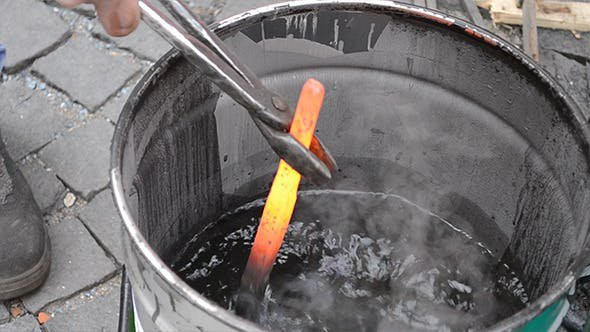
\includegraphics[width=0.3\linewidth]{figs/VN12-Y24-PH-SYL-003-2}
	\captionof{figure}{Miếng sắt nung được thả vào chậu nước}
\end{center}
\subsubsection{Định luật I nhiệt động lực học}
\begin{boxdl}
	Độ biến thiên nội năng của hệ bằng tổng công và nhiệt lượng mà hệ nhận được:
	\begin{equation}
		\Delta U= A+Q
	\end{equation}
\end{boxdl}
Trong đó:
\begin{itemize}
	\item $\Delta U$: độ biến thiên nội năng của hệ, đơn vị trong hệ SI là joule $\left(\si{\joule}\right)$;
	\item $A$: công mà hệ nhận/thực hiện, đơn vị trong hệ SI là joule $\left(\si{\joule}\right)$;
	\begin{itemize}[label=+]
		\item $A>0$: hệ nhận công;
		\item $A<0$: hệ thực hiện công.
	\end{itemize}
	\item $Q$: nhiệt lượng hệ trao đổi với bên ngoài, đơn vị trong hệ SI là joule $\left(\si{\joule}\right)$;
	\begin{itemize}[label=+]
		\item $Q>0$: hệ nhận nhiệt lượng;
		\item $Q<0$: hệ truyền nhiệt lượng.
	\end{itemize}
\end{itemize}
\begin{center}
	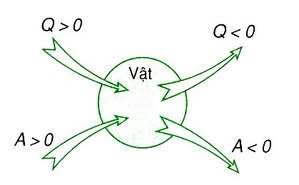
\includegraphics[width=0.35\linewidth]{figs/VN12-Y24-PH-SYL-003-3}
	\captionof{figure}{Quy ước về dấu của $Q$ và $A$}
\end{center}
\subsection{VÍ DỤ MINH HOẠ}
\begin{dang}{Trình bày được các cách làm thay đổi nội năng}
	
\end{dang}
		\begin{vd}
		Dựa vào mô hình động học phân tử, hãy giải thích hiện tượng quả bóng bàn bị móp (nhưng chưa bị thủng) khi thả vào cốc nước nóng sẽ phồng trở lại.
			\begin{center}
				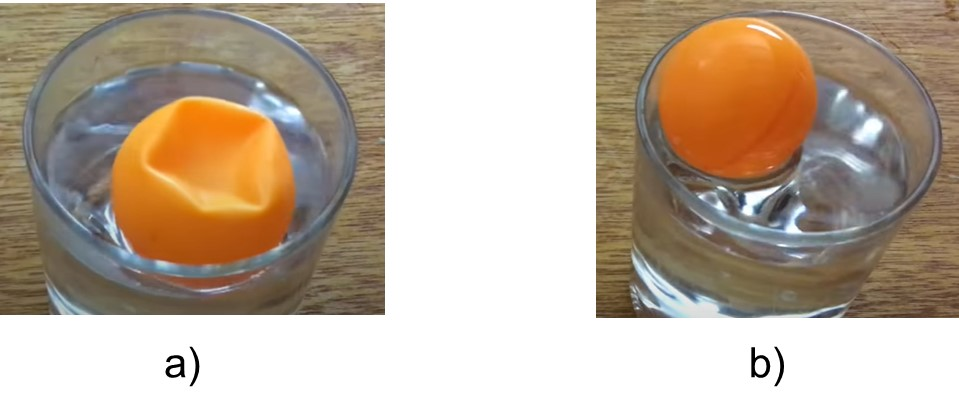
\includegraphics[width=0.45\linewidth]{{figs/VN12-Y24-PH-SYL-003-4}}
				\captionof{figure}{a) Quả bóng bàn ban đầu bị móp; b) Quả bóng sau khi được ngâm vào cốc nước nóng}
			\end{center}
			\loigiai{
				Khi thả quả bóng bi móp vào nước nóng, nhiệt độ khí trong quả bóng tăng làm các phân tử khí chuyển động nhiệt nhanh hơn nên va chạm với thành bóng nhiều hơn và mạnh hơn. Khi đó, áp suất khí trong quả bóng tăng lên và tạo ra lực đẩy đủ lớn làm vỏ cao su của quả bóng phồng trở lại}
	\end{vd}
		
		\begin{vd}
			Vì sao pha nước chanh bằng nước ấm thì đường sẽ tan nhanh hơn khi pha bằng nước lạnh? Em còn cách làm nào khác để đường tan nhanh hơn không? Hãy đưa ra lời giải thích cho cách làm của em.
			\loigiai{Khi nhiệt độ càng cao thì động năng chuyển động nhiệt của các phân tử nước và phân tử đường càng lớn. Do đó, các phân tử đường dễ dàng hoà tan vào trong nước.\\
				Để đường tan nhanh vào nước ta có thể khuấy mạnh vào nước. Khi đó, hệ nước và đường nhận công nên động năng chuyển động của các phân tử đường và nước tăng. Các phân tử đường dễ hoà tan vào nước}
		\end{vd}
	\begin{dang}{Vận dụng định luật I nhiệt động lực học}
		\end{dang}
		\begin{vd}
			Giả sử cung cấp cho hệ nhiệt động một công là $\SI{200}{\joule}$ nhưng nhiệt lượng mà hệ bị thất thoát ra ngoài môi trường là $\SI{120}{\joule}$. Hỏi nội năng của hệ tăng hay giảm bao nhiêu?
			\loigiai{Hệ nhận công nên $A>0\Rightarrow A=\SI{200}{\joule}$.\\
				Hệ toả nhiệt ra ngoài môi trường nên $Q<0\Rightarrow Q=\SI{-120}{\joule}$.\\
				Độ biến thiên nội năng của hệ:
				$$\Delta U= Q+A=\SI{80}{\joule}.$$
				Vậy nội năng của hệ tăng $\SI{80}{\joule}.$}
		\end{vd}
		\begin{vd}
		Cung cấp nhiệt lượng $\SI{1.5}{\joule}$ cho một khối khí trong một cylanh đặt nằm ngang. Chất khí nở ra, đẩy piston đi một đoạn $\SI{5}{\centi\meter}$. Biết lực ma sát giữa piston và cylanh có độ lớn là $\SI{20}{\newton}$, coi piston chuyển động thẳng đều. Tính
		\begin{enumerate}[label=\alph*)]
			\item Công của khối khí thực hiện.
			\item Độ biến thiên nội năng của khối khí.
		\end{enumerate}
		\loigiai{
			\begin{enumerate}[label=\alph*)]
				\item Do piston chuyển động thẳng đều nên lực đẩy $\vec{F}$ của khối khí tác dụng lên lên piston cân bằng với lực ma sát giữa piston và cylanh.\\
				Độ lớn công của khối khí thực hiện là:
				$$A'=F\cdot d=F_\text{ms}\cdot d=\left(\SI{20}{\newton}\right)\cdot\left(\SI{0.05}{\meter}\right)=\SI{1}{\joule}.$$
				\item Vì khối khí thực hiện công nên $A<0$: $A=-A'=\SI{-1}{\joule}$.\\
				Khối khí nhận nhiệt nên $Q>0\Rightarrow Q=\SI{1.5}{\joule}$.\\
				Độ biến thiên nội năng của khối khí:
				$$\Delta U=Q+A=\SI{1.5}{\joule}-\SI{1}{\joule}=\SI{0.5}{\joule}.$$
				Vậy nội năng của khối khí tăng $\SI{0.5}{\joule}$.
		\end{enumerate}}
		\end{vd}
		
		\begin{vd}
			Khi truyền nhiệt lượng $Q$ cho khối khí trong một cylanh hình trụ thì khí dãn nở đẩy piston làm thể tích của khối khí tăng thêm 7 lít. Biết áp suất của khối khí là $\SI{3E5}{\pascal}$ và không đổi trong quá trình khí dãn nở. Tính
			\begin{enumerate}[label=\alph*)]
				\item Công mà khối khí thực hiện.
				\item Nhiệt lượng cung cấp cho khối khí. Biết rằng trong quá trình này, nội năng của khối khí giảm $\SI{1100}{\joule}$.
			\end{enumerate}
		\loigiai{
			\begin{enumerate}[label=\alph*)]
				\item Độ lớn công khối khí thực hiện:
				$$A'=F\cdot d=p\cdot S\cdot d=p\cdot\Delta V=\left(\SI{3E5}{\pascal}\right)\cdot\left(\SI{7E-3}{\meter^3}\right)=\SI{2100}{\joule}.$$
				\item Vì khối khí thực hiện công nên $A<0$: $A=-A'=\SI{-2100}{\joule}$.\\
				Nội năng của khí giảm nên $\Delta U<0\Rightarrow \Delta U=\SI{-1100}{\joule}$.\\
				Áp dụng định luật I nhiệt động lực học, nhiệt lượng cần cung cấp cho khối khí:
				$$Q=\Delta U - A=\SI{-1100}{\joule}+\SI{2100}{\joule}=\SI{1000}{\joule}.$$
			\end{enumerate}
		}
		\end{vd}
	\subsection{BÀI TẬP TRẮC NGHIỆM}
	\Opensolutionfile{ans}[ans/G12Y24B3TN]
	\begin{ex}
		Khi nhiệt độ của vật tăng lên thì
		\choice
		{\True động năng của các phân tử cấu tạo nên vật tăng}
		{động năng của các phân tử cấu tạo nên vật giảm}
		{nội năng của vật tăng}
		{thế năng của các phân tử cấu tạo nên vật tăng}
		\loigiai{ }
		\end{ex}
% ==================================================================================
	\begin{ex}
Nội năng của một hệ là 
	\choice
	{\True tổng động năng chuyển động nhiệt và thế năng tương tác giữa các phân tử cấu tạo nên hệ}
	{tổng của động năng và thế năng của hệ}
	{tổng động năng chuyển động của các phân tử cấu tạo nên hệ}
	{tổng động lượng chuyển động hỗn loạn và thế năng tương tác giữa các phân tử cấu tạo nên hệ}
	\loigiai{ }
\end{ex}
% ==================================================================================
	\begin{ex}
	Nội năng của một hệ phụ thuộc vào
	\choice
	{nhiệt độ của hệ}
	{thể tích của hệ}
	{\True nhiệt độ và thể tích của hệ}
	{nhiệt độ, thể tích và khối lượng của hệ}
	\loigiai{ }
\end{ex}
% ==================================================================================
	\begin{ex}
Cách làm thay đổi nội năng của hệ bằng hình thức thực hiện công là
	\choice
	{bỏ thỏi sắt vào nước nóng}
	{\True chà sát miếng kim loại bằng giấy nhám}
	{đưa một thỏi sắt lên cao}
	{hơ thỏi sắt bằng đèn cồn}
	\loigiai{ }
\end{ex}
% ==================================================================================
	\begin{ex}
Khi ấn piston để nén khí trong một cylanh thì
	\choice
	{kích thước mỗi phân tử khí giảm}
	{\True khoảng cách giữa các phân tử khí giảm}
	{khối lượng mỗi phân tử khí giảm}
	{số phân tử khí giảm}
	\loigiai{ }
\end{ex}
% ==================================================================================
	\begin{ex}
	Định luật I của nhiệt động lực học là vận dụng định luật nào sau đây?
	\choice
	{Định luật bảo toàn động lượng}
	{Định luật bảo toàn cơ năng}
	{\True Định luật bảo toàn và chuyển hoá năng lượng}
	{Các định luật Newton về chuyển động}
	\loigiai{ }
\end{ex}
% ==================================================================================
	\begin{ex}
	Khi nói về nội dung của định luật I nhiệt động lực học, phát biểu nào sau đây là \textbf{sai}?
	\choice
	{Vật nhận nhiệt, nội năng của vật tăng}
	{Vật truyền nhiệt, nội năng của vật giảm}
	{Độ biến thiên nội năng của vật bằng tổng công và nhiệt lượng mà vật nhận được}
	{\True Độ biến thiên nội năng của vật bằng hiệu giữa công và nhiệt lượng mà vật nhận được}
	\loigiai{ }
\end{ex}
% ==================================================================================
	\begin{ex}
			Hệ thức $\Delta U=Q+A$ khi $Q>0$ và $A<0$ mô tả quá trình
		\choice
		{hệ truyền nhiệt và sinh công}
		{\True hệ nhận nhiệt và sinh công}
		{hệ truyền nhiệt và nhận công}
		{hệ nhận nhiệt và nhận công}
		\loigiai{ }
	\end{ex}
% ==================================================================================
		\begin{ex}
			Dùng tay nén piston và đồng thời nung nóng khối khí trong cylanh. Xác định dấu của $Q$ và $A$ của khối khí trong biểu thức của định luật I nhiệt động lực học $\Delta U=Q+A$.
		\choice
		{\True $A>0$; $Q>0$}
		{$A<0$; $Q>0$}
		{$A>0$; $Q<0$}
		{$A<0$; $Q<0$}
		\loigiai{ }
	\end{ex}
	% ==================================================================================
		\begin{ex}
		Chọn phát biểu \textbf{đúng nhất}.
	\choice
	{Động cơ nhiệt là động cơ trong đó toàn bộ phần năng lượng của nhiên liệu bị đốt cháy chuyển hoá thành cơ năng}
	{Động cơ nhiệt là động cơ trong đó một phần năng lượng của nhiên liệu bị đốt cháy chuyển hoá thành nhiệt năng}
	{\True Động cơ nhiệt là động cơ trong đó một phần năng lượng của nhiên liệu bị đốt cháy chuyển hoá thành cơ năng}
	{Động cơ nhiệt là động cơ trong đó toàn bộ năng lượng của nhiên liệu bị đốt cháy chuyển hoá thành nhiệt năng}
	\loigiai{ }
\end{ex}
% ==================================================================================

	\begin{ex}
	Khi thả một thỏi kim loại đã được nung nóng vào một chậu nước lạnh thì nội năng của thỏi kim loại và của nước thay đổi như thế nào?
	\choice
	{Nội năng của thỏi kim loại và của nước đều tăng}
	{Nội năng của thỏi kim loại và của nước đều giảm}
	{\True Nội năng của thỏi kim loại giảm, nội năng của nước tăng}
	{Nội năng của thỏi kim loại tăng, nội năng của nước giảm}
	\loigiai{ }
\end{ex}
% ==================================================================================
	\begin{ex}
	Khi ôtô đóng kín cửa để ngoài trời nắng nóng, nhiệt độ không khí trong xe tăng rất cao so với nhiệt độ bên ngoài, làm giảm tuổi thọ các thiết bị trong xe. Nguyên nhân gây ra sự tăng nhiệt độ này là do thể tích khối khí trong ôtô
	\choice
	{thay đổi nên nhiệt lượng mà khối khí trong ôtô nhận được chủ yếu làm tăng nội năng của khối khí}
	{không đổi nên nhiệt lượng mà khối khí trong ôtô nhận được chủ yếu làm giảm nội năng của khối khí}
	{thay đổi nên nhiệt lượng mà khối khí trong ôtô nhận được chủ yếu làm tăng nội giảm của khối khí}
	{không đổi nên nhiệt lượng mà khối khí trong ôtô nhận được chủ yếu làm tăng nội năng của khối khí}
	\loigiai{ }
\end{ex}
% ==================================================================================
	\begin{ex}
		Người ta thực hiện công $\SI{100}{\joule}$ để nén khí trong một cylanh. Biết trong quá trình nén, khí truyền ra ngoài môi trường nhiệt lượng $\SI{20}{\joule}$. Độ biến thiên nội năng của khí là 
		\choice
		{\True $\SI{80}{\joule}$}
		{$\SI{-80}{\joule}$}
		{$\SI{120}{\joule}$}
		{$\SI{60}{\joule}$}
		\loigiai{Khí nhận công nên $A>0\Rightarrow A=\SI{100}{\joule}$, khí toả nhiệt ra ngoài nên $Q<0\Rightarrow Q=\SI{-20}{\joule}$.\\
			Độ biến thiên nội năng của khí:
			$$\Delta U=Q+A=\SI{80}{\joule}.$$ }
	\end{ex}
% ==================================================================================
	\begin{ex}
	Khi truyền nhiệt lượng $\SI{6E6}{\joule}$ cho khí trong một cylanh hình trụ thì khí nở ra đẩy piston lên làm thể tích của khí tăng thêm $\SI{0.50}{\meter^3}$. Biết áp suất của khí là $\SI{8E6}{\newton/\meter^2}$ và coi áp suất này không đổi trong quá trình khí thực hiện công. Độ biến thiên nội năng của khí là
	\choice
	{$\SI{3E6}{\joule}$}
	{$\SI{1.5E6}{\joule}$}
	{\True $\SI{2E6}{\joule}$}
	{$\SI{3.5E6}{\joule}$}
	\loigiai{Công do khí thực hiện:
		$$A'=F\Delta x=pS\Delta x=p\Delta V=\SI{4E6}{\joule}.$$
		Vì khí thực hiện công nên $A<0\Rightarrow A=-A'=-\SI{4E6}{\joule}$.\\
		Độ biến thiên nội năng của khí:
		$$\Delta U=Q+A=\SI{2E6}{\joule}.$$}
\end{ex}
% ==================================================================================
 
\begin{ex}
Một khối khí chứa trong một cylanh đặt thẳng đứng, miệng cylanh được đậy kín bằng một piston nhẹ có tiết diện $\SI{10}{\centi\meter^2}$, có thể dịch chuyển không ma sát trong cylanh. Người ta kéo đều piston lên cao một đoạn $\SI{10}{\centi\meter}$. Biết nhiệt độ khối khí không đổi, áp suất khí quyển bằng $\SI{101325}{\pascal}$ và công do khối khí sinh ra trong quá trình này là $\SI{7.5}{\joule}$. Công cần thực hiện để kéo piston là
	\choice
	{$\SI{2.31}{\joule}$}
	{\True $\SI{2.63}{\joule}$}
	{$\SI{17.63}{\joule}$}
	{$\SI{7.5}{\joule}$}
	\loigiai{\begin{center}
			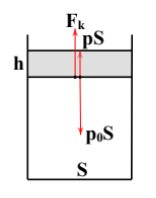
\includegraphics[width=0.25\linewidth]{figs/VN12-Y24-PH-SYL-003P-2}
		\end{center}
		Piston được nâng lên đều nên:
		$$F_k=\left(p_0-p\right)S.$$
		Công cần thực hiện:
		$$A=F_k\Delta h=\left(p_0-p\right)S\Delta h=p_0S\Delta h-A_\text{khí}=\SI{2.6325}{\joule}.$$}
\end{ex}
	\Closesolutionfile{ans}
\subsection{TRẮC NGHIỆM ĐÚNG/SAI}
\setcounter{ex}{0}
\begin{ex}
	Trong quá trình nóng chảy của vật rắn
	\begin{enumerate}[label=\alph*)]
		\item Nhiệt được truyền vào vật rắn để làm tăng nhiệt độ của nó.
		\item Động năng trung bình của các phân tử trong vật rắn giảm đi.
		\item Nội năng của vật rắn không thay đổi.
		\item Tại nhiệt độ nóng chảy, nội năng không thay đổi.
	\end{enumerate}
\loigiai{
\begin{enumerate}[label=\alph*)]
	\item Đúng.
	\item Sai. Động năng trung bình của các phân tử trong vật rắn tăng lên.
	\item Sai. Nội năng của vật rắn thay đổi.
	\item Đúng. Nội năng không thay đổi tại nhiệt độ nóng chảy, vì năng lượng được sử dụng để làm tan chảy các liên kết giữa các phân tử mà không làm thay đổi nhiệt độ.
\end{enumerate}
}
	\end{ex}
% ====================================================================================
\begin{ex}
	Bố trí thí nghiệm như hình bên. Dùng đèn cồn đun nóng ống nghiệm cho đến khi nút bấc bật ra.
	\begin{center}
		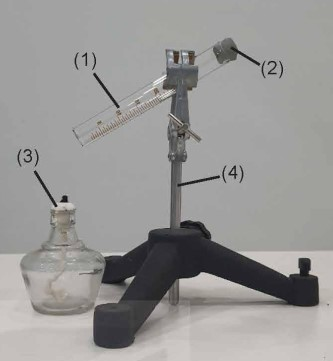
\includegraphics[width=0.3\linewidth]{figs/VN12-Y24-PH-SYL-003P-5}
	\end{center}
	\begin{enumerate}[label=\alph*)]
		\item Khi nút chưa bị bật ra, nội năng của không khí trong ống nghiệm không thay đổi.
		\item Nội năng của không khí trong ống nghiệm tăng không chỉ do động năng chuyển động nhiệt của các phân tử khí tăng mà còn do thế năng tương tác giữa chúng tăng.
		\item Nút bấc bị ra là kết quả của áp suất bên trong ống nghiệm giảm đi.
		\item Quá trình nút bấc bật ra ngoài thì khí trong ống đang thực hiện công.
	\end{enumerate}
\loigiai{
\begin{enumerate}[label=\alph*)]
	\item Sai. Nội năng khí trong ống tăng do nhận nhiệt.
	\item Sai. Thế năng tương tác giữa các phân tử phụ thuộc khoảng cách giữa các phân tử, không phụ thuộc vào nhiệt độ.
	\item Sai. Nút bấc bị ra là kết quả của áp suất bên trong ống nghiệm tăng lên.
	\item Đúng.
\end{enumerate}
}
	\end{ex}

% ====================================================================================
\begin{ex}
		Khối khí được chứa trong cylanh, bên trên được nút kín bằng piston cách nhiệt như hình bên dưới. Dùng tay ấn mạnh piston đồng thời nung nóng bên dưới cylanh bằng ngọn lửa đèn cồn.
	\begin{center}
		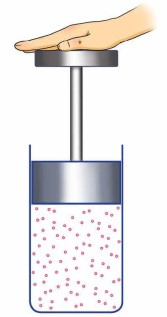
\includegraphics[width=0.15\linewidth]{figs/VN12-Y24-PH-SYL-003P-3}
	\end{center}
	\begin{enumerate}[label=\alph*)]
		\item $A>0$ vì khí nhận công (khí bị nén).
		\item $Q<0$ vì khí bị nung nóng.
		\item Nội năng của khí trong cylanh tăng.
		\item Động năng chuyển động nhiệt của các phân tử khí giảm.
	\end{enumerate}
\loigiai{
\begin{enumerate}[label=\alph*)]
	\item Đúng.
	\item Sai. Khí nhận nhiệt nên $Q>0$.
	\item Đúng.
	\item Sai. Động năng chuyển động nhiệt của các phân tử khí tăng.
\end{enumerate}
}
	

	\end{ex}

% =================================================================================
\begin{ex}
	Khi kéo đi kéo lại sợi dây cuốn quanh một ống nhôm đựng nước nút kín, người ta thấy nước trong ống nóng lên rồi sôi, hơi nước đẩy nút bật ra cùng một lớp hơi nước trắng do các hạt nước rất nhỏ tạo thành.
	\begin{center}
		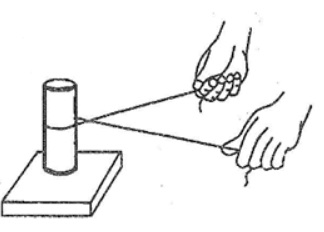
\includegraphics[width=0.3\linewidth]{figs/VN12-Y24-PH-SYL-003P-4}
	\end{center}
	\begin{enumerate}[label=\alph*)]
		\item Ống nhôm nóng lên (nội năng ông nhôm tăng) do nhận công.
		\item Có sự truyền nhiệt từ ống nhôm vào nước, làm cho nước nóng lên và hoá hơi.
		\item Quá trình hơi nước làm bật nút là quá trình hơi nước thực hiện công.
		\item Nếu thay nước bằng rượu thì nút sẽ lâu bật ra hơn.
	\end{enumerate}
\loigiai{
\begin{enumerate}[label=\alph*)]
	\item Đúng.
	\item Đúng.
	\item Đúng.
	\item Sai. Nhiệt độ sôi của rượu thấp hơn nước nên rượu dễ hoá hơi hơn. Quá trình làm nút bật ra sẽ diễn ra nhanh hơn.
\end{enumerate}
}
	\end{ex}

% ====================================================================================
\begin{ex}
	Hằng ngày, Mặt Trời truyền về Trái Đất dưới hình thức bức xạ nhiệt một lượng năng lượng khổng lồ, lớn gấp khoảng 20 000 lần tổng năng lượng mà con người sử dụng. 
	\begin{center}
		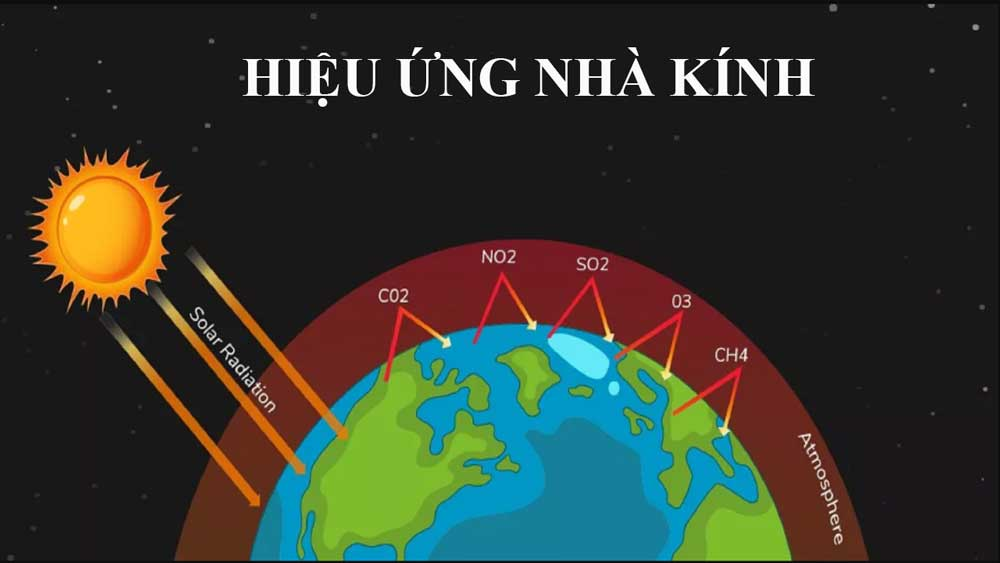
\includegraphics[width=0.45\linewidth]{figs/VN12-Y24-PH-SYL-003P-6}
	\end{center}
	Trái Đất hấp thụ một phần năng lượng này, đồng thời phản xạ lại một phần dưới hình thức bức xạ nhiệt của Trái Đất. Bầu khí quyển bao quanh Trái Đất có tác dụng giống như một nhà lợp kính, giữ lại bức xạ nhiệt của Trái Đất làm cho bề mặt của Trái Đất và không khí bao quanh Trái Đất bị nóng lên. Do sự tương tự đó mà hiệu ứng này của bầu khí quyền được gọi là hiệu ứng nhà kính khí quyển, gọi tắt là hiệu ứng nhà kính.\\
	Trong khí quyển thì khí carbon dioxide $\left(\ce{CO_2}\right)$ đóng vai trò chủ yếu trong việc gây ra hiệu ứng nhà kính. Hiệu ứng nhà kính vừa có thể có ích vừa có thể có hại. Hiện nay, người ta đang cố gắng làm giảm hiệu ứng nhà kính để ngăn không cho nhiệt độ trên Trái Đất tăng lên quá nhanh, làm đe doạ cuộc sống của con người và các sinh vật khác trên hành tinh này.\\
	Nhận định các phát biểu sau đây: 
	\begin{enumerate}[label=\alph*)]
		\item Khí nhà kính có vai trò giữ cho nhiệt độ trên Trái Đất không quá lạnh.
		\item Tăng sử dụng động cơ đốt trong có thể làm giảm hiệu ứng nhà kính.
		\item Một phần nguyên nhân của nước biển dâng là do nhiệt độ trên Trái Đất tăng làm cho nước biển bốc hơi nhiều và gây ra mưa nhiều.
		\item Hiệu ứng nhà kính giúp điều hòa nhiệt độ trên Trái Đất, giúp giảm hạn hán và lũ lụt, giảm băng tan trên địa cực và nước biển dâng cao.
	\end{enumerate}
\loigiai{
\begin{enumerate}[label=\alph*)]
	\item Đúng.
	\item Sai.
	\item Sai.
	\item Sai.
\end{enumerate}
}
	\end{ex}

\subsection{BÀI TẬP TỰ LUẬN}
\setcounter{ex}{0}
\begin{ex}
		Khi đang đóng đinh vào gỗ, mũ đinh có nóng lên nhưng rất ít. Khi đinh đã đóng chắc vào gỗ rồi (không lún thêm được nữa), chỉ cần đóng thêm vài nhát búa là mũ đinh nóng lên rất nhiều. Hãy giải thích?
		\loigiai{
		Khi đang đóng đinh, công thực hiện chuyển thành động năng cho đinh và nội năng cho đinh và búa. Nhưng khi đinh đã được đóng chặt vào gỗ, công thực hiện chỉ chuyển thành nội năng, do đó làm đinh nóng lên nhanh hơn.
	}
	\end{ex}
% ====================================================================================
\begin{ex}
	\immini{
	Hiện nay, kính cường lực (kính chịu lực rất tốt) thường được sử dụng để làm một phần tường của các toà nhà, trung tâm thương mại, \dots thay thế vật liệu gạch, bê tông.\\
	Tuy nhiên, vào những ngày nắng nóng, nếu bước vào những căn phòng có tường làm bằng kính cường lực bị đóng kín, ta thường thấy không khí trong phòng nóng hơn so với bên ngoài.
	\begin{enumerate}[label=\alph*)]
		\item Tại sao không khí trong phòng nóng hơn so với không khí ngoài trời?
		\item Hãy đề xuất các biện pháp đơn giản để làm giảm sự tăng nhiệt của không khí trong phòng vào những ngày mùa hè.
	\end{enumerate}
}{	
\includegraphics[scale=0.3]{figs/VN12-Y24-PH-SYL-003P-1}
}
\loigiai{
\begin{enumerate}[label=\alph*)]
	\item Vào mùa hè, do mặt trời chiếu sáng, không khí trong phòng nhận nhiệt lượng $\left(Q>0\right)$. Do phòng đóng kín nên thể tích khí không đổi, khối khí không sinh công $\left(A=0\right)$. Theo định luật I nhiệt động lực học: $\Delta U=Q+A>0$, nên nội năng của khối khí tăng, làm nhiệt độ không khí trong phòng tăng. Do đó, không khí trong phòng nóng hơn ngoài trời.
	\item Biện pháp đơn giản làm giảm sự tăng nhiệt độ của không khí trong phòng:
	\begin{itemize}
		\item Mở cửa để không khí đối lưu với bên ngoài, từ đó làm nội năng của không khí trong phòng giảm và nhiệt độ phòng giảm xuống.
		\item Lắp rèm cửa: Rèm thường bằng vải dày chuyên dụng, màu sẫm, bề mặt lượn sóng. Khi ánh sáng mặt trời đi qua rèm nó vừa bị phản xạ (do bề mặt, do chất liệu vải), vừa bị hấp thụ (do màu sắc, độ dày của vải). Bên cạnh đó, giữa rèm và mặt kính có có một khoảng ngăn cách, lớp không khí này có khả năng ngăn một phần sự truyền nhiệt từ bên ngoài vào phòng (do không khí dẫn nhiệt kém). Các yếu tố trên làm hạn chế khả năng truyền nhiệt trực tiếp từ Mặt Trời vào sâu bên trong phòng, làm nhiệt độ trong phòng tăng chậm hơn.
		\item Dán tấm phim cách nhiệt: Phim cách nhiệt thường có cấu tạo đặc biệt (từ nhiều lớp polyester và chống ánh sáng tử ngoại), nên khi ánh sáng mặt trời chiếu vào, tấm phim cách nhiệt vừa có tác dụng phản xạ (chủ yếu với ánh sáng hồng ngoại), vừa có tác dụng hấp thụ ánh sáng (chủ yếu với ánh sáng tử ngoại) và truyền qua với các ánh sáng dịu với mắt.
	\end{itemize}
\end{enumerate}
}
	\end{ex}
% ====================================================================================
\begin{ex}
	Thực hiện công $\SI{150}{\joule}$ để nén khí trong một cylanh thì khí truyền ra môi trường xung quanh nhiệt lượng $\SI{30}{\joule}$. Xác định độ thay đổi nội năng của khí trong cylanh.
	\loigiai{
	Khí nhận công nên $A>0\Rightarrow A=\SI{150}{\joule}$, khí truyền nhiệt nên $Q<0\Rightarrow Q=\SI{-30}{\joule}$.\\
	Độ biến thiên nội năng của khí:
	$$\Delta U=Q+A=\SI{120}{\joule}.$$
}
	\end{ex}

% ====================================================================================
\begin{ex}
	Giả sử một người đang thực hiện bài vận động vất vả chẳng hạn như nâng tạ hoặc đạp xe. Cơ thể đang thực hiện công và đồng thời nhiệt lượng thoát ra ngoài qua lỗ chân lông vào không khí xung quanh. Theo định luật I nhiệt động lực học, nhiệt độ cơ thể sẽ giảm dần trong quá trình tập luyện. Tuy nhiên, điều đó lại không xảy ra. Như vậy, có phải định luật I nhiệt động lực học không đúng trong trường hợp này phải không? Hãy giải thích.
	\loigiai{
	Trong quá trình vận động cơ thể con người thực hiện công và toả nhiệt ra ngoài môi trường nhưng trong cơ thể người luôn có năng lượng dự trữ để cung cấp năng cho các hoạt động của cơ thể. Năng lượng dự trữ này có được do các quá trình biến đổi chất dinh dưỡng từ thức ăn. Vì vậy, cơ thể luôn được duy trì ở nhiệt độ ổn định và định luật I nhiệt động lực học trong trường hợp này vẫn được nghiệm đúng.
}
	\end{ex}

% ===================================================================================
\begin{ex}
	Một quả bóng khối lượng $\SI{200}{\gram}$ rơi từ độ cao $\SI{15}{\meter}$ xuống sân và nảy lên được $\SI{10}{\meter}$. Độ biến thiên nội năng của quả bóng là bao nhiêu? Lấy $g=\SI{10}{\meter/\second^2}$.
	\loigiai{
	Độ biến thiên nội năng của quả bóng:
	$$\Delta U=mg\left(h-h'\right)=\SI{10}{\joule}.$$
}
\end{ex}

% ===================================================================================
\begin{ex}
	Một vật khối lượng $\SI{1}{\kilogram}$ trượt không vận tốc đầu từ đỉnh xuống chân một mặt phẳng dài $\SI{21}{\meter}$, nghiêng $\SI{30}{\degree}$ so với mặt nằm ngang. Tốc độ của vật ở chân mặt phẳng nghiêng là $\SI{4.1}{\meter/\second}$. Tính công của lực ma sát và độ biến thiên nội năng của vật trong quá trình chuyển động trên. Lấy $g=\SI{9.8}{\meter/\second^2}$. Bỏ qua sự trao đổi nhiệt với mặt phẳng nghiêng.
	\loigiai{
		Công của lực ma sát:
		$$A_\text{ms}=W_\text{s}-W_\text{t}=mgh_\text{s}+\dfrac{1}{2}mv^2_\text{s}-mgh_\text{t}-\dfrac{1}{2}mv^2_\text{t}=\dfrac{1}{2}mv^2_\text{s}-mg\ell\sin\SI{30}{\degree}\approx\SI{-94.5}{\joule}.$$
		Độ biến thiên nội năng của vật trong quá trình chuyển động bằng công của lực ma sát:
		$$\Delta U=\SI{94.5}{\joule}.$$
	}
\end{ex}
	
%\newpage\section{NHIỆT DUNG RIÊNG}
\subsection{LÝ THUYẾT TRỌNG TÂM}
\subsubsection{Nhiệt dung riêng}
\begin{boxdn}
	Nhiệt dung riêng của một chất là nhiệt lượng cần cung cấp để nhiệt độ của $\SI{1}{\kilogram}$ chất đó tăng thêm $\SI{1}{\kelvin}$.
\end{boxdn}
Đơn vị đo của nhiệt dung riêng trong hệ SI là $\si{\joule/\left(\kilogram\cdot\kelvin\right)}$, nhiệt dung riêng kí hiệu là $c$.
\subsubsection{Nhiệt lượng trao đổi để khối chất thay đổi nhiệt độ}
\begin{boxdn}
	Nhiệt lượng trao đổi (toả ra hay nhận vào) để khối chất thay đổi nhiệt độ từ $T_1$ đến nhiệt độ $T_2$:
	$$Q=mc\Delta T$$
\end{boxdn}
với:
\begin{itemize}
	\item $Q$: nhiệt lượng trao đổi, đơn vị trong hệ SI là $\si{\joule}$;
	\item $m$: khối lượng, đơn vị trong hệ SI là $\si{\kilogram}$;
	\item $c$: nhiệt dung riêng của chất tạo nên vật, đơn vị trong hệ SI là $\si{\joule/\left(\kilogram\cdot\kelvin\right)}$;
	\item $\Delta T=T_2-T_1$: độ biến thiên nhiệt độ, đơn vị trong hệ SI là $\si{\kelvin}$.
\end{itemize}
\subsubsection{Trạng thái cân bằng nhiệt của hệ nhiệt động}
\begin{boxdn}
	Hệ nhiệt động đạt trạng thái cân bằng nhiệt khi tổng nhiệt lượng trao đổi trong hệ bằng 0:
	$$\sum Q=Q_1+Q_2+\dots+Q_n=0.$$
\end{boxdn}
\subsection{VÍ DỤ MINH HOẠ}
\begin{dang}{Xác định nhiệt lượng trao đổi để khối chất thay đổi nhiệt độ}
	\end{dang}
	\begin{vd}
		Hãy giải thích tại sao ban ngày có gió mát thổi từ biển vào đất liền? Biết rằng nhiệt dung riêng của đất và nước vào khoảng $\SI{800}{\joule/\left(\kilogram\cdot\kelvin\right)}$ và $\SI{4200}{\joule/\left(\kilogram\cdot\kelvin\right)}$.
	\loigiai{Vào ban ngày, vì nhiệt dung riêng của nước cao hơn nhiệt dung riêng của đất nên với cùng nhiệt lượng nhận từ Mặt Trời thì nước biển có độ tăng nhiệt độ thấp hơn đất liền. Do hiện tượng đối lưu, luồng không khí từ biển sẽ thổi vào đất liền. Lúc này có sự trao đổi nhiệt lượng giữa không khí trong đất liền và không khí từ biển thổi vào làm giảm nhiệt độ không khí ở đất liền. Do đó, chúng ta sẽ cảm thấy mát hơn}

	\end{vd}
	
	
\begin{vd}
Một thùng đựng $\SI{20}{\ell}$ nước ở nhiệt độ $\SI{20}{\celsius}$. Cho khối lượng riêng của nước là $\SI{1000}{\kilogram\cdot\meter^{-3}}$, nhiệt dung riêng của nước $c=\SI{4200}{\joule/\left(\kilogram\cdot\kelvin\right)}$.
			\begin{enumerate}[label=\alph*)]
				\item Tính nhiệt lượng cần truyền cho nước trong thùng để nhiệt độ của nó tăng lên tới $\SI{70}{\celsius}$.
				\item Tính thời gian truyền nhiệt lượng cần thiết nếu dùng một thiết bị điện có công suất $\SI{2.5}{\kilo\watt}$ để đun lượng nước trên. Biết chỉ có $\SI{80}{\percent}$ điện năng tiêu thụ được dùng để làm nóng nước.
			\end{enumerate}
	\loigiai{
				\begin{enumerate}[label=\alph*)]
					\item Khối lượng của $\SI{20}{\ell}$ nước:
					$$m=\rho V=\left(\SI{1000}{\kilogram\cdot\meter^{-3}}\right)\cdot\left(\SI{20E-3}{\meter^{3}}\right)=\SI{20}{\kilogram}.$$
					Nhiệt lượng cần truyền cho nước trong thùng để nhiệt độ của nó tăng lên tới $\SI{70}{\celsius}$:
					$$Q=mc\Delta t=\left(\SI{20}{\kilogram}\right)\cdot\left[\SI{4200}{\joule/\left(\kilogram\cdot\kelvin\right)}\right]\cdot\left(\SI{50}{\kelvin}\right)=\SI{42E5}{\joule}.$$
					\item Năng lượng thiết bị điện tiêu thụ để truyền được nhiệt lượng cần thiết đun nóng nước đến $\SI{70}{\celsius}$:
					$$W=\dfrac{Q}{H}=\SI{52.5E5}{\joule}.$$
					Thời gian đun nước:
					$$t=\dfrac{W}{\calP}=\dfrac{\SI{52.5E5}{\joule}}{\SI{2.5E3}{\watt}}=\SI{2100}{\second}=\SI{35}{\minute}.$$
				\end{enumerate}}
		
\end{vd}
\begin{dang}{Vận dụng phương trình cân bằng nhiệt}
	\end{dang}
\begin{vd}
		Một bác thợ rèn nhúng một con dao rựa bằng thép có khối lượng $\SI{1.1}{\kilogram}$ ở nhiệt độ $\SI{850}{\celsius}$ vào trong bể nước lạnh để làm tăng độ cứng của lưỡi dao. Nước trong bể có thể tích $\SI{200}{\ell}$ và có nhiệt độ bằng nhiệt độ ngoài trời là $\SI{27}{\celsius}$. Xác định nhiệt độ của nước khi có sự cân bằng nhiệt. Bỏ qua sự truyền nhiệt cho thành bể, môi trường bên ngoài và bỏ qua quá trình nước hoá hơi khi vừa tiếp xúc với rựa. Biết nhiệt dung riêng của thép là $\SI{460}{\joule/\left(\kilogram\cdot\kelvin\right)}$; của nước là $\SI{4180}{\joule/\left(\kilogram\cdot\kelvin\right)}$.
\loigiai{
			Gọi $t_\text{cb}$ là nhiệt độ của nước khi có sự cân bằng nhiệt.\\
			Hệ đạt trạng thái cân bằng nhiệt khi tổng nhiệt lượng trao đổi trong hệ bằng 0:
			\begin{eqnarray*}
				&&	Q_\text{rựa}+Q_\text{nước}=0\\
				&\Leftrightarrow&	m_\text{t}c_\text{t}\left(t_\text{cb}-t_\text{t}\right)+m_\text{n}c_\text{n}\left(t_\text{cb}-t_\text{n}\right)=0\\
				&\Rightarrow& t_\text{cb}=\dfrac{m_\text{n}c_\text{n}t_\text{n}+m_\text{t}c_\text{t}t_\text{t}}{m_\text{n}c_\text{n}+m_\text{t}c_\text{t}}\approx\SI{27.5}{\celsius}.
			\end{eqnarray*}
		}
\end{vd}
	
\begin{vd}
Một bình nhiệt lượng kế bằng nhôm có khối lượng $m_1=\SI{200}{\gram}$ chứa $m_2=\SI{400}{\gram}$ nước ở nhiệt độ $t_1=\SI{20}{\celsius}$. Đổ thêm vào bình một khối lượng nước $m$ ở nhiệt độ $t_2=\SI{5}{\celsius}$. Khi cân bằng nhiệt thì nhiệt độ của nước trong bình là $t=\SI{10}{\celsius}$. Cho biết nhiệt dung riêng của nhôm là $c_1=\SI{880}{\joule/\left(\kilogram\cdot\kelvin\right)}$, của nước là $c_2=\SI{4200}{\joule/\left(\kilogram\cdot\kelvin\right)}$. Bỏ qua sự trao đổi nhiệt với môi trường. Xác định giá trị của $m$.
\loigiai{Khi hệ đạt trạng thái cân bằng nhiệt thì tổng nhiệt lượng trao đổi của hệ bằng 0:
			$$mc_2\left(t-t_2\right)+m_1c_1\left(t-t_1\right)+m_2c_2\left(t-t_1\right)=0$$
			\begin{eqnarray*}
				\Rightarrow m&=&\dfrac{m_1c_1\left(t-t_1\right)+m_2c_2\left(t-t_1\right)}{c_2\left(t_2-t\right)}\\
				&=&\dfrac{\left\{\left(\SI{0.2}{\kilogram}\right)\cdot\left[\SI{880}{\joule/\left(\kilogram\cdot\kelvin\right)}\right]+\left(\SI{0.4}{\kilogram}\right)\cdot\left[\SI{4200}{\joule/\left(\kilogram\cdot\kelvin\right)}\right]\right\}\cdot\left(\SI{10}{\celsius}-\SI{20}{\celsius}\right)}{\left[\SI{4200}{\joule/\left(\kilogram\cdot\kelvin\right)}\right]\cdot\left(\SI{5}{\celsius}-\SI{10}{\celsius}\right)}\\
				&\approx&\SI{0.88}{\kilogram}.
			\end{eqnarray*}
		}
\end{vd}
\subsection{BÀI TẬP TRẮC NGHIỆM}
\setcounter{ex}{0}
\Opensolutionfile{ans}[ans/G12Y24B4TN]
% ===================================================================
\begin{ex}
	Nhiệt lượng vật trao đổi để thay đổi nhiệt độ phụ thuộc vào
	\choice
	{khối lượng, thể tích và độ thay đổi nhiệt độ của vật}
	{ thể tích, nhiệt độ ban đầu và chất cấu tạo nên vật}
	{\True  khối lượng của vật, chất cấu tạo nên vật và độ thay đổi nhiệt độ của vật}
	{nhiệt độ ban đầu, nhiệt độ lúc sau và áp suất của môi trường}
	\loigiai{ }
	\end{ex}
% ===================================================================
\begin{ex}
	Có 4 bình A, B, C, D đều đựng nước ở cùng một nhiệt độ với thể tích tương ứng là: 1 lít, 2 lít, 3 lít, 4 lít. Sau
	khi dùng các đèn cồn giống hệt nhau để đun các bình này khác nhau. Bình có nhiệt độ thấp nhất là
	\begin{center}
		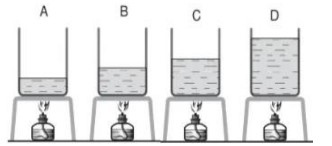
\includegraphics[width=0.4\linewidth]{figs/VN12-Y24-PH-SYL-004P-1}
	\end{center}
	\choice
	{bình A}
	{bình B}
	{bình C}
	{\True bình D}
	\loigiai{}
\end{ex}
% ===================================================================
\begin{ex}
Có 4 bình A, B, C, D đều đựng nước ở cùng một nhiệt độ với thể tích tương ứng là: 1 lít, 2 lít, 3 lít, 4 lít. Sau
khi dùng các đèn cồn giống hệt nhau để đun các bình này khác nhau. Bình có nhiệt độ cao nhất là
\begin{center}
	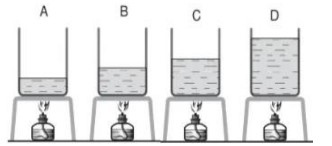
\includegraphics[width=0.4\linewidth]{figs/VN12-Y24-PH-SYL-004P-1}
\end{center}
	\choice
	{\True bình A}
	{bình B}
	{bình C}
	{bình D}
	\loigiai{}
\end{ex}
% ===================================================================
\begin{ex}
	Chọn phát biểu \textbf{sai}.\\
	Nhiệt dung riêng của một chất 
	\choice
	{là nhiệt lượng cần truyền để $\SI{1}{\kilogram}$ chất đó tăng thêm $\SI{1}{\celsius}$}
	{\True phụ thuộc vào khối lượng riêng của chất đó}
	{phụ thuộc vào bản chất của chất đó}
	{có đơn vị là $\si{\joule/\kilogram\cdot\kelvin}$}
	\loigiai{}
\end{ex}
% ===================================================================
\begin{ex}
Nhiệt độ của vật nào tăng lên nhiều nhất khi ta thả rơi bốn vật dưới đây có cùng khối lượng và từ cùng một độ cao xuống đất? Coi như toàn bộ cơ năng của vật chuyển hoá thành nhiệt năng.
	\choice
	{Vật bằng nhôm, có nhiệt dung riêng là $\SI{880}{\joule/\kilogram\cdot\kelvin}$}
	{Vật bằng đồng, có nhiệt dung riêng là $\SI{380}{\joule/\kilogram\cdot\kelvin}$}
	{\True Vật bằng chì, có nhiệt dung riêng là $\SI{120}{\joule/\kilogram\cdot\kelvin}$}
	{Vật bằng gang, có nhiệt dung riêng là $\SI{5500}{\joule/\kilogram\cdot\kelvin}$}
	\loigiai{$$\Delta t=\dfrac{Q}{mc}.$$
		Vì chì có nhiệt dung riêng nhỏ nhất nên có độ tăng nhiệt độ nhiều nhất}
\end{ex}
% ===================================================================
\begin{ex}
	Tính nhiệt lượng do miếng sắt khối lượng $\SI{2}{\kilogram}$ toả ra khi hạ nhiệt độ từ $\SI{500}{\celsius}$ xuống còn $\SI{40}{\celsius}$. Biết nhiệt dung riêng của sắt là $\SI{478}{\joule/\left(\kilogram\cdot\kelvin\right)}$
	\choice
	{$\SI{219880}{\joule}$}
	{\True $\SI{439760}{\joule}$}
	{$\SI{879520}{\joule}$}
	{$\SI{109940}{\joule}$}
	\loigiai{
		Nhiệt lượng miếng sắt toả ra:
		$$Q=mc\left(t_1-t_2\right)=\SI{439760}{\joule}.$$	
	}
\end{ex}
% ===================================================================
\begin{ex}
	Một viên đạn bằng bạc đang bay với tốc độ $\SI{200}{\meter/\second}$ thì va chạm vào một bức tường gỗ và nằm yên trong bức tường. Nhiệt dung riêng của bạc là $\SI{234}{\joule/\left(\kilogram\cdot\kelvin\right)}$. Nếu coi viên đạn không trao đổi nhiệt với bên ngoài thì nhiệt độ của viên đạn sẽ tăng thêm bao nhiêu độ?
	\choice
	{$\SI{58}{\celsius}$}
	{$\SI{171}{\celsius}$}
	{\True $\SI{85}{\celsius}$}
	{$\SI{250}{\celsius}$}
	\loigiai{
		Áp dụng định luật bảo toàn và chuyển hoá năng lượng:
		$$\dfrac{1}{2}mv^2=mc\Delta t\Rightarrow \Delta t=\dfrac{v^2}{2c}\approx\SI{85}{\celsius}.$$	
	}
\end{ex}
% ===================================================================
\begin{ex}
	Người ta cọ xát hai vật với nhau, nhiệt dung của hai vật là $\SI{800}{\joule/\kelvin}$. Sau 1 phút người ta thấy nhiệt độ của mỗi vật tăng thêm $\SI{30}{\kelvin}$. Công suất trung bình của việc cọ xát bằng
	\choice
	{$\SI{1080}{\watt}$}
	{$\SI{980}{\watt}$}
	{$\SI{480}{\watt}$}
	{\True $\SI{800}{\watt}$}
	\loigiai{	Công suất trung bình của việc cọ xát là
		$$\calP=\dfrac{2c\Delta T}{t}=\SI{800}{\watt}.$$}
\end{ex}
% ===================================================================
\begin{ex}
	Đầu thép của một búa máy có khối lượng $\SI{12}{\kilogram}$ nóng lên thêm $\SI{20}{\celsius}$ sau 1,5 phút hoạt động. Biết rằng  $\SI{40}{\percent}$ cơ năng của búa máy chuyển thành nhiệt năng của đầu búa. Nhiệt dung riêng của thép là $\SI{460}{\joule/\kilogram\cdot\kelvin}$. Công suất của búa gần nhất với giá trị nào sau đây?
	\choice
	{\True $\SI{3}{\kilo\watt}$}
	{$\SI{4}{\kilo\watt}$}
	{$\SI{5}{\kilo\watt}$}
	{$\SI{6}{\kilo\watt}$}
	\loigiai{		Công suất toả nhiệt trên đầu búa:
		$$\calP_\text{hp}=\dfrac{mc\Delta T}{t}\approx\SI{1226.67}{\watt}.$$
		Công suất của búa:
		$$\calP=\dfrac{\calP_\text{hp}}{0,4}\approx\SI{3.066}{\kilo\watt}.$$}
\end{ex}
% ===================================================================
\begin{ex}
	\immini{Quả cầu kim loại được làm bằng chất có nhiệt dung riêng $c=\SI{460}{\joule/\left(\kilogram\cdot\kelvin\right)}$ được treo bởi sợi day có chiều dài $\ell=\SI{46}{\centi\meter}$. Quả cầu được nâng lên đến B rồi thả rơi. Sau khi chạm tường, nó bật lên đến C $\left(\alpha=\SI{60}{\degree}\right)$. Biết rằng $\SI{60}{\percent}$ độ giảm thế năng của quả cầu biến thành nhiệt làm nóng quả cầu. Lấy $g=\SI{10}{\meter/\second^2}$. Độ tăng nhiệt độ của quả cầu là
\choice
{\True $\SI{3E-3}{\celsius}$}
{$\SI{6E-3}{\celsius}$}
{$\SI{1.5E-3}{\celsius}$}
{Không đủ dữ kiện để xác định}	
}{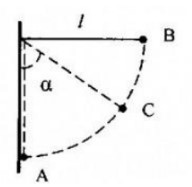
\includegraphics[scale=0.8]{figs/VN12-Y24-PH-SYL-004P-2}
}
	\loigiai{Độ tăng nhiệt độ của quả cầu:
		$$\Delta t=\dfrac{0,6mg\ell\cos\SI{60}{\degree}}{mc}=\dfrac{0,6g\ell\cos\SI{60}{\degree}}{c}=\SI{3E-3}{\celsius}.$$}
\end{ex}
% ===================================================================
\begin{ex}
	Có hai quả cầu bằng chì giống nhau có nhiệt dung riêng là $c$, chuyển động đến va chạm mềm trực diện với tốc độ lần lượt là $v$ và $2v$. Cho rằng toàn bộ cơ năng mất mát trong quá trình va chạm chuyển hoá thành nhiệt năng làm nóng hai quả cầu. Độ tăng nhiệt độ của hai quả cầu là
		\choice
		{\True $\dfrac{9v^2}{8c}$}
		{$\dfrac{7v^2}{8c}$}
		{$\dfrac{9v^2}{7c}$}
		{$\dfrac{11v^2}{7c}$}
	\loigiai{Tốc độ hai quả cầu sau va chạm:
		$$V=\dfrac{2mv-mv}{2m}=0,5v.$$
		Nhiệt lượng toả ra trong quá trình va chạm:
		$$Q=\dfrac{1}{2}mv^2+\dfrac{1}{2}m\left(2v\right)^2-\dfrac{1}{2}\cdot 2mV^2=\dfrac{9}{4}mv^2.$$
		Độ tăng nhiệt độ của hai quả cầu:
		$$\Delta t=\dfrac{Q}{2mc}=\dfrac{9v^2}{8c}.$$}
\end{ex}
% ===================================================================
\begin{ex}
Một lượng nước và một lượng rượu có thể tích bằng nhau, được cung cấp nhiệt lượng tương ứng là $Q_1$ và $Q_2$. Biết khối lượng riêng của nước là $\SI{1000}{\kilogram/\meter^3}$ và của rượu là $\SI{800}{\kilogram/\meter^3}$, nhiệt dung riêng của nước là $\SI{4200}{\joule/\kilogram\cdot\kelvin}$ và của rượu là $\SI{2500}{\joule/\kilogram\cdot\kelvin}$. Để độ tăng nhiệt độ của nước và rượu bằng nhau thì
	\choice
	{$Q_1=Q_2$}
	{$Q_1=1,25Q_2$}
	{$Q_1=1,68Q_2$}
	{\True $Q_1=2,1Q_2$}
	\loigiai{	$$\dfrac{Q_1}{Q_2}=\dfrac{m_1c_1\Delta t}{m_2c_2\Delta t}=\dfrac{D_1c_1}{D_2c_2}=2,1.$$}
\end{ex}
% ===================================================================
\begin{ex}
	Một ấm đồng khối lượng $\SI{300}{\gram}$ chứa 1 lít nước ở nhiệt độ $\SI{15}{\celsius}$. Biết trung bình mỗi giây bếp truyền cho ấm một nhiệt lượng là $\SI{500}{\joule}$. Bỏ qua sự hao phí về nhiệt ra môi trường xung quanh. Lấy nhiệt dung riêng của đồng là $\SI{380}{\joule/\kilogram\cdot\kelvin}$ và của nước là $\SI{4186}{\joule/\kilogram\cdot\kelvin}$. Thời gian đun sôi ấm nước có giá trị gần đúng là
	\choice
	{\True 12 phút}
	{13 phút}
	{14 phút}
	{15 phút}
	\loigiai{Nhiệt lượng nước và ấm cần thu vào để sôi:
		$$Q=\left(m_1c_1+m_2c_2\right)\Delta t=\SI{365500}{\joule}.$$
		Thời gian đun sôi ấm nước:
		$$t=\dfrac{Q}{\SI{500}{\joule/\second}}=\SI{731}{\second}\approx\SI{12}{\text{phút}}.$$}
\end{ex}
% ===================================================================
\begin{ex}
	Người ta muốn pha nước tắm với nhiệt độ $\SI{38}{\celsius}$ thì phải pha bao nhiêu lít nước sôi vào 15 lít nước lạnh ở $\SI{24}{\celsius}$?
	\choice
	{2,5 lít}
	{\True 3,38 lít}
	{4,2 lít}
	{5 lít}
	\loigiai{$$Q_1+Q_2=0\Leftrightarrow V_1\rho c\left(t_\text{cb}-t_1\right)+V_2\rho c\left(t_\text{cb}-t_2\right)=0$$
		$$\Leftrightarrow V_1\left(38-100\right)+15\cdot\left(38-24\right)=0\Rightarrow V_1=\SI{3.38}{\liter}.$$}
\end{ex}
% ===================================================================
\begin{ex}
	Một ấm đun nước bằng nhôm có khối lượng $\SI{400}{\gram}$, chứa 3 lít nước được đun trên bếp. Khi nhận thêm nhiệt lượng $\SI{740}{\kilo\joule}$ thì ấm đạt đến nhiệt độ $\SI{80}{\celsius}$. Biết nhiệt dung riêng của nhôm và nước lần lượt là $c_1=\SI{880}{\joule/\left(\kilogram\cdot\kelvin\right)}$, $c_2=\SI{4190}{\joule/\left(\kilogram\cdot\kelvin\right)}$. Nhiệt độ ban đầu của ấm là
	\choice
	{$\SI{8.15}{\celsius}$}
	{$\SI{8.15}{\kelvin}$}
	{\True $\SI{22.7}{\celsius}$}
	{$\SI{22.7}{\kelvin}$}
	\loigiai{$$Q=\left(m_1c_1+m_2c_2\right)\Delta t\Rightarrow \Delta t=\dfrac{Q}{m_1c_1+m_2c_2}\approx\SI{57.27}{\celsius}.$$
		Nhiệt độ ban đầu của ấm:
		$$t_1=t_2-\Delta t=\SI{22.73}{\celsius}.$$}
\end{ex}
% ===================================================================
\begin{ex}
Thả một miếng thép $\SI{2}{\kilogram}$ đang ở nhiệt độ $\SI{345}{\celsius}$ vào một bình đựng 3 lít nước. Sau khi cân bằng nhiệt, nhiệt độ cuối cùng của nước là $\SI{30}{\celsius}$. Bỏ qua sự trao đổi nhiệt với môi trường. Nhiệt dung riêng của thép và nước lần lượt là $\SI{460}{\joule/\kilogram\cdot\kelvin}$, $\SI{4200}{\joule/\kilogram\cdot\kelvin}$. Nhiệt độ ban đầu của nước là
	\choice
	{\True $\SI{7}{\celsius}$}
	{$\SI{17}{\celsius}$}
	{$\SI{27}{\celsius}$}
	{$\SI{37}{\celsius}$}
	\loigiai{Khi hệ đạt trạng thái cân bằng nhiệt thì tổng nhiệt lượng trao đổi trong hệ bằng 0:
		$$m_1c_1\left(t-t_1\right)+m_2c_2\left(t-t_2\right)=0$$
		$$\Leftrightarrow 2\cdot460\cdot\left(\SI{30}{\celsius}-\SI{345}{\celsius}\right)+3\cdot 4200\left(\SI{30}{\celsius}-t_2\right)=0\Rightarrow t_2=\SI{7}{\celsius}.$$}
\end{ex}
% ===================================================================
\begin{ex}
Thả một quả cầu nhôm khối lượng $\SI{0.15}{\kilogram}$ được đun nóng tới $\SI{100}{\celsius}$ vào một cốc nước ở $\SI{20}{\celsius}$. Sau một thời gian, nhiệt độ của quả và nước đều bằng $\SI{25}{\celsius}$. Coi quả cầu và nước chỉ trao đổi nhiệt cho nhau và bỏ qua quá trình nước hoá hơi khi tiếp xúc với bề mặt quả cầu. Cho nhiệt dung riêng của nhôm và nước lần lượt là $\SI{800}{\joule/\kilogram\cdot\kelvin}$, $\SI{4200}{\joule/\kilogram\cdot\kelvin}$. Khối lượng của nước là 
	\choice
	{$\SI{0.47}{\gram}$}
	{\True $\SI{0.43}{\kilo\gram}$}
	{$\SI{2}{\gram}$}
	{$\SI{2}{\kilo\gram}$}
	\loigiai{Khi cân bằng nhiệt, tổng nhiệt lượng trao đổi trong hệ bằng 0:
		$$m_1c_1\left(t-t_1\right)+m_2c_2\left(t-t_2\right)=0\Rightarrow m_2=\SI{0.4285}{\kilogram}.$$}
\end{ex}

% ===================================================================
\begin{ex}
	Thả một quả cầu bằng nhôm có khối lượng $\SI{0.21}{\kilogram}$ được nung nóng đến $\SI{200}{\celsius}$ vào cốc đựng nước ở $\SI{30}{\celsius}$. Sau một thời gian, nhiệt độ của nước và quả cầu đều bằng $\SI{50}{\celsius}$. Biết nhiệt dung riêng của nhôm là $\SI{880}{\joule/\left(\kilogram\cdot\kelvin\right)}$, nhiệt dung riêng của nước là $\SI{4200}{\joule/\left(\kilogram\cdot\kelvin\right)}$. Khối lượng nước trong cốc là	
	\choice
	{$\SI{3.3}{\kilogram}$}
	{$\SI{7.5}{\kilogram}$}
	{$\SI{0.21}{\kilogram}$}
	{\True $\SI{0.33}{\kilogram}$}
	\loigiai{
		Áp dụng phương trình cân bằng nhiệt:
		$$m_1c_1\left(t_\text{cb}-t_1\right)+m_2c_2\left(t_\text{cb}-t_2\right)=0$$
		$$\Rightarrow m_2=\dfrac{m_1c_1\left(t_\text{cb}-t_1\right)}{c_2\left(t_2-t_\text{cb}\right)}=\SI{0.33}{\kilogram}.$$ }
	
\end{ex}
% ===================================================================
\begin{ex}
	Người ta thả một miếng đồng có khối lượng $m_1=\SI{0.2}{\kilogram}$ được đốt nóng đến nhiệt độ $t_1$ vào một nhiệt lượng kế chứa $m_2=\SI{0.28}{\kilogram}$ nước ở nhiệt độ $t_2=\SI{20}{\celsius}$. Nhiệt độ khi có cân bằng nhiệt là $t_3=\SI{80}{\celsius}$. Biết nhiệt dung riêng của đồng và nước lần lượt là $c_1=\SI{400}{\joule/\left(\kilogram\cdot\kelvin\right)}$, $c_2=\SI{4200}{\joule/\left(\kilogram\cdot\kelvin\right)}$. Bỏ qua sự trao đổi nhiệt với nhiệt lượng kế và với môi trường. Nhiệt độ ban đầu $t_1$ của đồng là
	\choice
	{$\SI{926}{\celsius}$}
	{\True $\SI{962}{\celsius}$}
	{$\SI{530}{\celsius}$}
	{$\SI{503}{\celsius}$}
	\loigiai{
		Áp dụng phương trình cân bằng nhiệt:
		$$m_1c_1\left(t_3-t_1\right)+m_2c_2\left(t_3-t_2\right)=0\Rightarrow t_1=\SI{962}{\celsius}.$$
	}
\end{ex}
% ===================================================================
\begin{ex}
	Một bình nhiệt lượng kế bằng thép khối lượng $\SI{0.1}{\kilogram}$ chứa $\SI{0.5}{\kilogram}$ nước ở nhiệt độ $\SI{15}{\celsius}$. Người ta thả một miếng chì và một miếng nhôm có tổng khối lượng $\SI{0.15}{\kilogram}$ và nhiệt độ $\SI{100}{\celsius}$ vào nhiệt lượng kế. Kết quả là nhiệt độ của nước trong nhiệt lượng kế tăng lên đến $\SI{17}{\celsius}$. Cho biết nhiệt dung riêng của chì là $\SI{127.7}{\joule/\left(
		\kilogram\cdot\kelvin\right)}$, của nhôm là $\SI{836}{\joule/\left(\kilogram\cdot\kelvin\right)}$, của thép là $\SI{460}{\joule/\left(\kelvin\cdot\kelvin\right)}$, của nước là $\SI{4180}{\joule/\left(\kilogram\cdot\kelvin\right)}$. Bỏ qua sự mất mát nhiệt ra bên ngoài. Khối lượng của miếng chì và miếng nhôm lần lượt \textbf{gần với giá trị nào nhất} sau đây?
	\choice
	{$\SI{46}{\gram}$ và $\SI{104}{\gram}$}
	{$\SI{110}{\gram}$ và $\SI{40}{\gram}$}
	{\True $\SI{104}{\gram}$ và $\SI{46}{\gram}$}
	{$\SI{40}{\gram}$ và $\SI{110}{\gram}$}
	\loigiai{
		Ta có:
		\begin{equation}
			m_{\ce{Pb}}+m_{\ce{Al}}=\SI{0.15}{\kilogram}
			\label{eq:D1-1}
		\end{equation}	
		Áp dụng phương trình cân bằng nhiệt:
		$$m_{\ce{Pb}}c_{\ce{Pb}}\left(t_\text{cb}-t_{\ce{Pb}}\right)+m_{\ce{Al}}c_{\ce{Al}}\left(t_\text{cb}-t_{\ce{Al}}\right)+m_\text{nlk}c_\text{nlk}\left(t_\text{cb}-t_\text{nlk}\right)+m_\text{n}c_\text{n}\left(t_\text{cb}-t_\text{n}\right)=0.$$
		\begin{equation}
			\Rightarrow 10599,1m_{\ce{Pb}}+69388m_{\ce{Al}}=4272
			\label{eq:D1-2}
		\end{equation}
		Từ (\ref{eq:D1-1}) và (\ref{eq:D1-2}), thu được:
		$\heva{
			m_{\ce{Pb}}\approx\SI{104}{\gram}\\
			m_{\ce{Al}}\approx\SI{46}{\gram}
		}$.
	}
\end{ex}

% ===================================================================
\begin{ex}
	Một nhiệt lượng kế bằng nhôm có khối lượng $m$ ở nhiệt độ $t_1=\SI{20}{\celsius}$. Cho vào nhiệt lượng kế một lượng nước có khối lượng $m$ ở nhiệt độ $t_2$. Khi có cân bằng nhiệt, nhiệt độ của nước giảm đi $\SI{12}{\celsius}$. Tiếp tục đổ thêm một chất lỏng khác có khối lượng $2m$ ở nhiệt độ $t_3=\SI{40}{\celsius}$ (chất lỏng này không tác dụng hoá học với nước) vào nhiệt lượng kế thì nhiệt độ cân bằng giảm đi $\SI{16}{\celsius}$ so với nhiệt độ cân bằng nhiệt lần thứ nhất. Biết nhiệt dung riêng của nhôm và nước lần lượt là $\SI{900}{\joule/\left(\kilogram\cdot\kelvin\right)}$ và $\SI{4200}{\joule/\left(\kilogram\cdot\kelvin\right)}$. Bỏ qua sự mất mát nhiệt ra môi trường. Nhiệt dung riêng của chất lỏng đã đổ thêm vào nhiệt lượng kế bằng	
	\choice
	{$\SI{4080}{\joule/\left(\kilogram\cdot\kelvin\right)}$}
	{\True $\SI{2040}{\joule/\left(\kilogram\cdot\kelvin\right)}$}
	{$\SI{9690}{\joule/\left(\kilogram\cdot\kelvin\right)}$}
	{$\SI{1133}{\joule/\left(\kilogram\cdot\kelvin\right)}$}
	\loigiai{
		Gọi $c_1$; $c_2$; $c_3$ lần lượt là nhiệt dung riêng của nhôm; nước và chất lỏng đang xác định.\\
		\begin{itemize}
			\item \textbf{Cân bằng nhiệt lần 1}\\
			Áp dụng phương trình cân bằng nhiệt:
			\begin{eqnarray*}
				&&mc_1(t_\text{cb}-t_1)+mc_2\Delta t_2=0\\
				&\Leftrightarrow& m\cdot\left(t_\text{cb}-20\right)-m\cdot4200\cdot12=0\\
				&\Rightarrow &t_\text{cb}=\SI{76}{\celsius}.
			\end{eqnarray*}
			\item  \textbf{Cân bằng nhiệt lần 2}\\
			Áp dụng phương trình cân bằng nhiệt:
			\begin{eqnarray*}
				&&\left(mc_1+mc_2\right)\cdot\Delta t_\text{cb}+2mc_3\left(t'_\text{cb}-t_3\right)=0\\
				&\Leftrightarrow& \left(900+4200\right)\cdot\left(-16\right)+2\cdot c_3\left(76-16-40\right)=0\\
				&\Rightarrow& c_3=\SI{2040}{\joule/\left(\kilogram\cdot\kelvin\right)}
			\end{eqnarray*}
		\end{itemize}	
	}
\end{ex}
\Closesolutionfile{ans}
\subsection{TRẮC NGHIỆM ĐÚNG/SAI}
\setcounter{ex}{0}
% ===================================================================
\begin{ex}
	\immini{
	Hình bên là sơ đồ bố trí thí nghiệm xác định nhiệt dung riêng của nước.
	\begin{enumerate}[label=\alph*)]
		\item Biến áp nguồn có nhiệm vụ duy trì hiệu điện thế giữa hai đầu mạch điện.
		\item Oát kế dùng để đo cường độ dòng điện qua mạch.
		\item Nhiệt lượng toả ra trên dây nung bằng nhiệt lượng do nước thu vào.
		\item Nhiệt lượng kế ngăn cản sự trao đổi nhiệt giữa chất đặt trong bình với môi trường.
	\end{enumerate}
}{
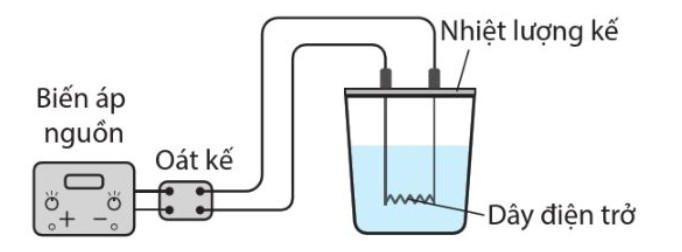
\includegraphics[scale=0.5]{figs/VN12-Y24-PH-SYL-004P-3}
}
\loigiai{
\begin{enumerate}[label=\alph*)]
	\item Đúng.
	\item Sai. Oát kế xác định công suất tiêu thụ điện của đoạn mạch.
	\item Đúng.
	\item Đúng.
\end{enumerate}
}
	\end{ex}

\begin{ex}
	Một chiếc thìa bằng đồng và một chiếc thìa bằng nhôm có cùng khối lượng và nhiệt độ ban đầu, được nhúng chìm vào cùng một cốc nước nóng (cao hơn nhiệt độ 2 thìa).
	\begin{enumerate}[label=\alph*)]
		\item 1 thìa toả nhiệt và 1 thìa thu nhiệt.
		\item Nhiệt độ cuối cùng của hai thìa bằng nhau.
		\item Khi có cân bằng nhiệt, nước bị giảm nhiệt độ.
		\item Nhiệt lượng của hai thìa trao đổi với nước là bằng nhau.
	\end{enumerate}
\loigiai{
\begin{enumerate}[label=\alph*)]
	\item Sai. Cả 2 thìa đều nhận nhiệt.
	\item Đúng.
	\item Đúng.
	\item Sai. Hai thìa có độ biến thiên nhiệt độ và khối lượng như nhau nhưng nhiệt dung riêng của chúng khác nhau nên nhiệt lượng trao đổi với nước của chúng khác nhau.
\end{enumerate}
}
	\end{ex}

\subsection{BÀI TẬP TỰ LUẬN}
\setcounter{ex}{0}
% ===================================================================
\begin{ex}
	\immini{
So sánh nhiệt dung riêng của thịt và của khoai tây, biết rằng khi cùng múc ra từ nồi canh hầm thì miếng thịt nguội nhanh hơn miếng khoai tây có cùng khối lượng.	

}{
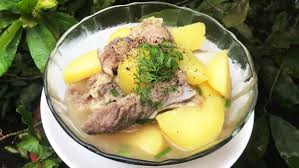
\includegraphics[scale=0.3]{figs/VN12-Y24-PH-SYL-004P-4}
}
\loigiai{
\begin{itemize}
	\item Nhiệt dung riêng là đại lượng thể hiện mức độ khó nóng, khó nguội của chất. Chất nào có nhiệt dung riêng lớn hơn thì khó nóng, khó nguội hơn.
	\item Khi cùng múc ra từ nồi canh hầm, miếng thịt nguội nhanh hơn miếng khoai tây cùng khối lượng. Điều này chứng tỏ thịt dễ nguội hơn khoai tây, nghĩa là nhiệt dung riêng của thịt nhỏ hơn nhiệt dung riêng của khoai tây.
\end{itemize}
}
	
	\end{ex}
% ===================================================================
\begin{ex}
Thùng nhôm khối lượng $\SI{1.2}{\kilogram}$ đựng $\SI{4}{\kilogram}$ nước ở $\SI{90}{\celsius}$. Cho biết nhiệt dung riêng của nhôm và nước lần lượt là $c_1=\SI{0.92}{\kilo\joule/\kilogram\cdot\kelvin}$, $c_2=\SI{4.186}{\kilo\joule/\left(\kilogram\cdot\kelvin\right)}$. Xác định nhiệt lượng thùng nước toả ra khi nhiệt độ giảm xuống còn $\SI{30}{\celsius}$.
	\loigiai{
	Nhiệt lượng do thùng nước toả ra:
	$$Q=\left(m_1c_1+m_2c_2\right)\Delta t=-\SI{1070880}{\joule}.$$
	Vậy nhiệt lượng do thùng nước toả ra là $\SI{1070880}{\joule}$.
	}
	
\end{ex}
% ===================================================================
\begin{ex}
	Để làm nguội nước nóng, người ta trộn $\SI{1.5}{\kilogram}$ nước ở $\SI{25}{\celsius}$ với $\SI{100}{\gram}$ nước ở $\SI{50}{\celsius}$. Xác định nhiệt độ cuối cùng của hỗn hợp khi cân bằng nhiệt.
	\loigiai{
	Khi có sự cân bằng nhiệt, tổng nhiệt lượng trao đổi trong hệ bằng 0:
	$$m_1c\left(t-t_1\right)+m_2c\left(t-t_2\right)=0$$
	$$\Leftrightarrow 1,5\left(t-\SI{25}{\celsius}\right)+0,1\left(t-\SI{50}{\celsius}\right)=0\Rightarrow t=\SI{26.5625}{\celsius}.$$
	}
	
\end{ex}
% ===================================================================
\begin{ex}
Muốn có nước ở nhiệt độ $t = \SI{50}{\celsius}$, người ta lấy $m_1 = \SI{3}{\kilogram}$ nước ở nhiệt độ $t_1 = \SI{100}{\celsius}$ trộn với nước ở nhiệt độ $t_2 =\SI{20}{\celsius}$. Hãy xác định khối lượng nước lạnh cần dùng.
	\loigiai{
		Khi cân bằng nhiệt, tổng nhiệt lượng trao đổi trong hệ bằng 0:
		$$m_1c\left(t_\text{cb}-t_1\right)+m_2c\left(t_\text{cb}-t_2\right)=0$$
		$$\Rightarrow m_2=\dfrac{m_1\left(t_1-t_\text{cb}\right)}{t_\text{cb}-t_2}=\SI{5}{\kilogram}.$$
	}
	
\end{ex}
% ===================================================================
\begin{ex}
Để xác định nhiệt dung riêng của một chất lỏng, người ta đổ chất lỏng đó vào $\SI{20}{\gram}$ nước ở nhiệt độ $\SI{100}{\celsius}$. Khi có cân bằng nhiệt, nhiệt độ của hỗn hợp đó là $\SI{37.5}{\celsius}$. Khối lượng hỗn hợp là $\SI{140}{\gram}$. Tính nhiệt dung riêng của chất lỏng đó, biết rằng nhiệt độ ban đầu của nó là $\SI{20}{\celsius}$ và hai chất lỏng không tác dụng hoá học với nhau. Cho nhiệt dung riêng của nước $c_2=\SI{4200}{\joule/\left(\kilogram\cdot\kelvin\right)}$.
	\loigiai{
	Gọi $m$ và $c$ lần lượt là khối lượng và nhiệt dung riêng của chất lỏng cần xác định nhiệt dung riêng.\\
	Khối lượng của chất lỏng đó:
	$$m=m_\text{hh}-m_\text{n}=\SI{120}{\gram}.$$
	Khi hệ đạt trạng thái cân bằng nhiệt thì tổng nhiệt lượng trao đổi của hệ bằng 0:
	$$mc\left(t_\text{cb}-t_0\right)+m_\text{n}c_\text{n}\left(t_\text{cb}-t_\text{0n}\right)=0$$
	$$\Rightarrow c=-\dfrac{m_\text{n}c_\text{n}\left(t_\text{cb}-t_\text{0n}\right)}{m\left(t_\text{cb}-t_0\right)}=\dfrac{\left(\SI{0.02}{\kilogram}\right)\cdot\left[\SI{4200}{\joule/\left(\kilogram\cdot\kelvin\right)}\right]\cdot\left(\SI{37.5}{\celsius}-\SI{100}{\celsius}\right)}{\left(\SI{0.12}{\kilogram}\right)\cdot\left(\SI{37.5}{\celsius}-\SI{20}{\celsius}\right)}=\SI{2500}{\joule/\left(\kilogram\cdot\kelvin\right)}.$$
	}
	
\end{ex}
% ===================================================================
\begin{ex}
	Để xác định nhiệt độ của một chiếc lò, người ta đốt nóng trong lò một cục sắt khối lượng $m_1=\SI{0.5}{\kilogram}$ rồi thả nhanh vào trong bình chứa $m_2=\SI{4}{\kilogram}$ nước có nhiệt độ ban đầu là $\SI{18}{\celsius}$. Nhiệt độ cuối cùng trong bình là $\SI{28}{\celsius}$. Hãy xác định nhiệt độ của lò. Bỏ qua trao đổi nhiệt với vỏ bình và quá trình nước hoá hơi khi tiếp xúc với cục sắt nóng. Cho nhiệt dung riêng của sắt là $c_1=\SI{460}{\joule/\left(\kilogram\cdot\kelvin\right)}$, nhiệt dung riêng của nước là $c_2=\SI{4200}{\joule/\left(\kilogram\cdot\kelvin\right)}$.
	\loigiai{
	Khi cân bằng nhiệt, tổng nhiệt lượng trao đổi trong hệ bằng 0:
	$$m_1c_1\left(t_\text{cb}-t_1\right)+m_2c_2\left(t_\text{cb}-t_2\right)=0\Rightarrow t_1\approx\SI{758.4}{\celsius}.$$
	}
	
\end{ex}
% ===================================================================
\begin{ex}
Trộn lẫn rượu vào nước, người ta thu được một hỗn hợp nặng $\SI{120.8}{\gram}$ ở nhiệt độ $\SI{30}{\celsius}$. Tính khối lượng nước và rượu đã pha, biết rằng ban đầu rượu ở nhiệt độ $\SI{10}{\celsius}$ và nước ở nhiệt độ $\SI{90}{\celsius}$. Cho nhiệt dung riêng của rượu và nước lần lượt là $\SI{2500}{\joule/\left(\kilogram\cdot\kelvin\right)}$, $\SI{4200}{\joule/\left(\kilogram\cdot\kelvin\right)}$.
	\loigiai{
		Gọi:
		\begin{itemize}
			\item $m_1, c_1, t_1$ lần lượt là khối lượng, nhiệt dung riêng và nhiệt độ ban đầu của rượu;
			\item $m_2, c_2, t_2$ lần lượt là khối lượng, nhiệt dung riêng và nhiệt độ ban đầu của nước.
		\end{itemize}
		Ta có:
		\begin{equation}
			\label{eq:4P-1}
			m_1+m_2=\SI{120.8}{\gram}=\SI{0.1208}{\kilogram}
		\end{equation}
		Khi hệ cân bằng nhiệt, tổng nhiệt lượng trao đổi trong hệ bằng 0:
		$$m_1c_1\left(t_\text{cb}-t_1\right)+m_2c_2\left(t_\text{cb}-t_2\right)=0$$
		\begin{equation}
			\label{eq:4P-2}
			50000m_1-252000m_2=0
		\end{equation}
		Từ (\ref{eq:4P-1}) và (\ref{eq:4P-2}) suy ra:
		\begin{equation*}
			\begin{cases}
				m_1=\SI{100.8}{\gram}\\
				m_2=\SI{20}{\gram}
			\end{cases}
			.
		\end{equation*}
	}
	
\end{ex}
% ===================================================================
\begin{ex}
	Bỏ một vật rắn khối lượng $\SI{100}{\gram}$ ở $\SI{100}{\celsius}$ vào $\SI{500}{\gram}$ nước ở $\SI{15}{\celsius}$ thì nhiệt độ sau cùng của vật là $\SI{16}{\celsius}$. Thay nước bằng $\SI{800}{\gram}$ chất lỏng khác ở $\SI{10}{\celsius}$ thì nhiệt độ sau cùng là $\SI{13}{\celsius}$. Tìm nhiệt dung riêng của vật rắn và chất lỏng. Cho nhiệt dung riêng của nước là $c = \SI{4200}{\joule/\left(\kilogram\cdot\kelvin\right)}$.
	\loigiai{
		\textbf{Khi bỏ vật rắn vào nước:}\\
		Khi cân bằng nhiệt, tổng nhiệt lượng trao đổi của vật rắn và nước bằng 0:
		$$m_vc_v\left(t_\text{cb}-t_v\right)+m_nc_n\left(t_\text{cb}-t_n\right)=0\Rightarrow c_v=\dfrac{m_nc_n\left(t_\text{cb}-t_n\right)}{m_v\left(t_v-t_\text{cb}\right)}=\SI{250}{\joule/\left(\kilogram\cdot\kelvin\right)}.$$
		\textbf{Khi bỏ vật rắn vào trong chất lỏng khác}\\
		Khi cân bằng nhiệt, tổng nhiệt lượng trao đổi của vật rắn và chất lỏng bằng 0:
		$$m_vc_v\left(t'_\text{cb}-t_v\right)+m_lc_l\left(t'_\text{cb}-t_l\right)\Rightarrow c_l=\dfrac{m_vc_v\left(t_v-t_\text{cb}\right)}{m_l\left(t'_\text{cb}-t_l\right)}=\SI{906.25}{\joule/\left(\kilogram\cdot\kelvin\right)}.$$
	}
	
\end{ex}
% ===================================================================
\begin{ex}
Người ta đổ $m_1 =\SI{200}{\gram}$ nước sôi có nhiệt độ $t_1 =\SI{100}{\celsius}$ vào một chiếc cốc có khối lượng $m_2 = \SI{120}{\gram}$ đang ở nhiệt độ $t_2 =\SI{20}{\celsius}$. sau khoảng thời gian $T = \SI{5}{\text{phút}}$, nhiệt độ của cốc nước bằng $t=\SI{40}{\celsius}$. Xem rằng sự mất nhiệt xảy ra một cách điều đặn, hãy xác định nhiệt lượng tỏa ra môi trường xung quanh trong mỗi giây. Cho nhiệt dung riêng nước và thuỷ tinh lần lượt là $c_1=\SI{4200}{\joule/\left(\kilogram\cdot\kelvin\right)}$, $c_2=\SI{840}{\joule/\left(\kilogram\cdot\kelvin\right)}$.
	\loigiai{Nhiệt lượng nước sôi toả ra để giảm nhiệt độ từ $\SI{100}{\celsius}$ còn $\SI{40}{\celsius}$:
		$$Q_\text{toả}=m_1c_1\left(t_1-t\right)=\SI{50400}{\joule}.$$
		Nhiệt lượng cốc thuỷ tinh thu vào để tăng nhiệt độ từ $\SI{20}{\celsius}$ lên $\SI{40}{\celsius}$:
		$$Q_\text{thu}=m_2c_2\left(t-t_2\right)=\SI{2016}{\joule}.$$
		Nhiệt lượng toả ra môi trường trong mỗi giây:
		$$w=\dfrac{Q_\text{toả}-Q_\text{thu}}{T}=\SI{161.28}{\joule/\second}.$$
	}
	
\end{ex}
% ===================================================================
\begin{ex}
	Trộn ba chất lỏng không tác dụng hoá học với nhau có khối lượng lần lượt là $m_1=\SI{2}{\kilogram}$, $m_2=\SI{3}{\kilogram}$, $m_3=\SI{4}{\kilogram}$. Biết nhiệt dung riêng và nhiệt độ ban đầu của mỗi chất lỏng lần lượt là $c_1=\SI{2000}{\joule/\left(\kilogram\cdot\kelvin\right)}$, $t_1=\SI{57}{\celsius}$, $c_2=\SI{4000}{\joule/\left(\kilogram\cdot\kelvin\right)}$, $t_2=\SI{63}{\celsius}$, $c_3=\SI{3000}{\joule/\left(\kilogram\cdot\kelvin\right)}$, $t_3=\SI{92}{\celsius}$. Nhiệt độ của hỗn hợp khi cân bằng nhiệt là bao nhiêu?
	\loigiai{Khi cân bằng nhiệt, tổng nhiệt lượng trao đổi trong hệ bằng 0:
		$$m_1c_1\left(t_\text{cb}-t_1\right)+m_2c_2\left(t_\text{cb}-t_2\right)+m_3c_3\left(t_\text{cb}-t_3\right)=0$$
		$$\Rightarrow t_\text{cb}=\dfrac{m_1c_1t_1+m_2c_2t_2+m_3c_3t_3}{m_1c_1+m_2c_2+m_3c_3}\approx\SI{74.6}{\celsius}.$$
	}
	
\end{ex}
% ===================================================================
\begin{ex}
	Một nhiệt lượng kế bằng nhôm có khối lượng $m_1 = \SI{100}{\gram}$ chứa $m_2 =\SI{400}{\gram}$ nước ở nhiệt độ $t_1 =\SI{10}{\celsius}$. Người ta thả vào nhiệt lượng kế một thỏi hợp kim nhôm và thiếc có khối lượng $m = \SI{200}{\gram}$ được nung nóng đến nhiệt độ $t_2 =\SI{120}{\celsius}$. Nhiệt độ cân bằng của hệ thống là $\SI{14}{\celsius}$. Tính khối lượng nhôm và thiếc có trong hợp kim. Cho nhiệt dung riêng của nhôm, nước, thiếc lần lượt là: $c_1 =\SI{900}{\joule/\left(\kilogram\cdot\kelvin\right)}$, $c_2=\SI{4200}{\joule/\left(\kilogram\cdot\kelvin\right)}$, $c_3 =\SI{230}{\joule/\left(\kilogram\cdot\kelvin\right)}$.
	\loigiai{Gọi $m_\text{nh}$, $m_\text{th}$ lần lượt là khối lượng của nhôm và thiếc trong hợp kim.\\
		Ta có:
		\begin{equation}
			\label{eq:4P-3}
			m_\text{nh}+m_\text{th}=\SI{0.2}{\kilogram}
		\end{equation}
		Khi hệ cân bằng nhiệt, tổng nhiệt lượng trao đổi trong hệ bằng 0:
		$$m_1c_1\left(t_\text{cb}-t_1\right)+m_2c_2\left(t_\text{cb}-t_1\right)+m_\text{nh}c_1\left(t_\text{cb}-t_2\right)+m_\text{th}c_3\left(t_\text{cb}-t_2\right)=0$$
		\begin{equation}
			\label{eq:4P-4}
			95400m_\text{nh}+24380m_\text{th}=7080
		\end{equation}
		Từ (\ref{eq:4P-3}) và (\ref{eq:4P-4}), suy ra:
		\begin{equation*}
			\begin{cases}
				m_\text{nh}\approx\SI{0.031}{\kilogram}\\
				m_\text{th}\approx\SI{0.169}{\kilogram}
			\end{cases}
		\end{equation*}
	}
	
\end{ex}
% ===================================================================
\begin{ex}
	Một khối sắt có khối lượng $m$ ở nhiệt độ $\SI{150}{\celsius}$ khi thả vào một bình nước thì làm nhiệt độ nước tăng từ $\SI{20}{\celsius}$ lên $\SI{60}{\celsius}$. Thả tiếp vào nước khối sắt thứ hai có khối lượng $\dfrac{m}{2}$ ở $\SI{100}{\celsius}$ thì nhiệt độ sau cùng của nước là bao nhiêu? Coi như chỉ có sự trao đổi nhiệt giữa khối sắt với nước và bỏ qua quá trình nước hoá thành hơi khi tiếp xúc với sắt nóng.
	\loigiai{	Gọi:
		\begin{itemize}
			\item $m_2$ là khối lượng nước trong bình;
			\item $c_1$, $c_2$ lần lượt là nhiệt dung riêng của sắt và nước;
			\item $t_1$, $t_2$ lần lượt là nhiệt độ ban đầu của thỏi sắt khối lượng $m$ và nước.
		\end{itemize}
		\textbf{Bỏ khối sắt khối lượng $m$ vào nước}\\
		Khi có cân bằng nhiệt, nhiệt lượng trao đổi trong hệ bằng 0:
		$$mc_1\left(t_\text{cb}-t_1\right)+m_2c_2\left(t_\text{cb}-t_2\right)=0\Rightarrow \dfrac{mc_1}{m_2c_2}=\dfrac{t_\text{cb}-t_2}{t_1-t_\text{cb}}=\dfrac{4}{9}.$$
		\textbf{Bỏ thêm khối sắt khối lượng $m/2$ vào nước}\\
		Khi có cân bằng nhiệt, nhiệt lượng trao đổi trong hệ bằng 0:
		$$\left(mc_1+m_2c_2\right)\left(t'_\text{cb}-t_\text{cb}\right)+\dfrac{m}{2}c_1\left(t'_\text{cb}-t'_1\right)=0$$
		$$\Rightarrow \Rightarrow t'_\text{cb}=\dfrac{mc_1\left(t_\text{cb}+\dfrac{t'_1}{2}\right)+m_2c_2t_\text{cb}}{1,5mc_1+m_2c_2}=\dfrac{\dfrac{4}{9}\cdot\left(\SI{60}{\celsius}+\SI{50}{\celsius}\right)+\SI{60}{\celsius}}{1,5\cdot\dfrac{4}{9}+1}\approx\SI{65.33}{\celsius}.$$
	}
	
\end{ex}
% ===================================================================
\begin{ex}
Có hai bình cách nhiệt. Bình 1 chứa $m_1 =\SI{2}{\kilogram}$ nước ở $t_1=\SI{20}{\celsius}$, bình 2 chứa $m_2 =\SI{4}{\kilogram}$ nước ở $t_2 =\SI{60}{\celsius}$. Người ta rót một lượng nước $m$ từ bình 1 sang bình 2, sau khi cân bằng nhiệt, người ta lại rót một lượng nước từ bình 2 sang bình 1. Nhiệt độ cân bằng ở bình 1 lúc này là $\SI{21.95}{\celsius}$.
\begin{enumerate}[label=\alph*)]
	\item Tính lượng nước $m$ rong mỗi lần rót và nhiệt độ cân bằng ở bình 2.
	\item Nếu tiếp tục thực hiện lần hai, tìm nhiệt độ cân bằng ở mỗi bình.
\end{enumerate}
	\loigiai{\begin{enumerate}[label=\alph*)]
			\item \begin{itemize}
				\item \textbf{Rót nước từ bình 1 sang bình 2}\\
				Khi cân bằng nhiệt, tổng nhiệt lượng trao đổi của $m$ và lượng nước ở bình 2 bằng 0:
				$$mc\left(t'_2-t_1\right)+m_2c\left(t'_2-t_2\right)=0$$
				\begin{equation}
					\label{eq:4P-5}
					m\left(t'_2-t_1\right)=m_2\left(t_2-t'_2\right)
				\end{equation}
				\item \textbf{Rót nước từ bình 2 sang bình 1}\\
				Khi cân bằng nhiệt, tổng nhiệt lượng trao đổi của $m$ và lượng nước ở bình 1 bằng 0:
				$$mc\left(t'_1-t\right)+\left(m_1-m\right)c\left(t'_1-t_1\right)=0$$
				\begin{equation}
					\label{eq:4P-6}
					m\left(t-t_1\right)=m_1\left(t'_1-t_1\right)
				\end{equation}
				Từ (\ref{eq:4P-5}) và (\ref{eq:4P-6}), suy ra:
				\begin{equation*}
					\begin{cases}
						t=\dfrac{m_2t_2-m_1\left(t'_1-t_1\right)}{m_2}\approx\SI{59}{\celsius}\\
						m=\dfrac{m_1m_2\left(t'_1-t_1\right)}{m_2\left(t_2-t_1\right)-m_1\left(t'_1-t_1\right)}\approx\SI{0.1}{\kilogram}
					\end{cases}
					.
				\end{equation*}
			\end{itemize}
			\item Thực hiện lần hai, nhiệt độ cân bằng của mỗi bình là
			$$t''_2=\dfrac{mt'_1+m_2t'_2}{m+m_2}=\SI{58.12}{\celsius};\quad t''_1=\dfrac{mt''_2+\left(m_1-m\right)t_1}{m_1}=\SI{23.76}{\celsius}.$$
		\end{enumerate}
	}
	
\end{ex}	
%\newpage\section{NHIỆT NÓNG CHẢY RIÊNG - NHIỆT HOÁ HƠI RIÊNG}
\subsection{LÝ THUYẾT TRỌNG TÂM}
\subsubsection{Nhiệt nóng chảy riêng}
\begin{boxdl}
	Nhiệt nóng chảy riêng của một chất rắn có giá trị bằng nhiệt lượng cần cung cấp cho $\SI{1}{\kilogram}$ chất đó chuyển từ thể rắn sang thể lỏng tại nhiệt độ nóng chảy:
	\begin{equation}
		\lambda=\dfrac{Q}{m}
	\end{equation}
\end{boxdl}
với
\begin{itemize}
	\item $\lambda$: nhiệt nóng chảy riêng, đơn vị trong hệ SI là $\si{\joule/\kilogram}$;
	\item $Q$: nhiệt lượng khối chất rắn thu vào để nóng chảy hoàn toàn, đơn vị trong hệ SI là $\si{\joule}$;
	\item $m$: khối lượng của khối chất rắn, đơn vị trong hệ SI là $\si{\kilogram}$.
\end{itemize}
\subsubsection{Nhiệt hoá hơi riêng}
\begin{boxdl}
	Nhiệt hoá hơi riêng của một chất lỏng có giá trị bằng nhiệt lượng cần cung cấp cho $\SI{1}{\kilogram}$ chất lỏng đó hoá hơi hoàn toàn ở nhiệt độ sôi:
	\begin{equation}
		L=\dfrac{Q}{m}
	\end{equation}
\end{boxdl}
với
\begin{itemize}
	\item $L$: nhiệt hoá hơi riêng, đơn vị trong hệ SI là $\si{\joule/\kilogram}$;
	\item $Q$: nhiệt lượng khối chất lỏng thu vào để hoá hơi hoàn toàn, đơn vị trong hệ SI là $\si{\joule}$;
	\item $m$: khối lượng của khối chất lỏng, đơn vị trong hệ SI là $\si{\kilogram}$.
\end{itemize}
\subsection{VÍ DỤ MINH HOẠ}
\begin{dang}{Vận dụng biểu thức xác định nhiệt nóng chảy riêng}
\end{dang}
\begin{vd}
Một nhà máy thép mỗi lần luyện được 35 tấn thép. Cho nhiệt nóng chảy riêng của thép là $\SI{2.77E5}{\joule/\kilogram}$.
		\begin{enumerate}[label=\alph*)]
			\item Tính nhiệt lượng cần cung cấp để làm nóng chảy thép trong mỗi lần luyện của nhà máy ở nhiệt độ nóng chảy.
			\item Giả sử nhà máy sử dụng khí đốt để nấu chảy thép trong lò thổi (nồi nấu thép). Biết khi đốt cháy hoàn toàn $\SI{1}{\kilogram}$ khí đốt thì nhiệt lượng toả ra là $\SI{44E6}{\joule}$. Xác định khối lượng khí đốt cần sử dụng.
		\end{enumerate}

	\loigiai{
			\begin{enumerate}[label=\alph*)]
				\item Nhiệt lượng cần cung cấp để làm nóng chảy thép trong mỗi lần luyện của nhà máy ở nhiệt độ nóng chảy:
				$$Q=m\lambda=\left(\SI{35E3}{\kilogram}\right)\cdot\left(\SI{2.77E5}{\joule/\kilogram}\right)=\SI{96.95E8}{\joule}$$
				\item Khối lượng khí đốt cần sử dụng để nhiệt lượng toả ra như ở câu a):
				$$m=\dfrac{Q}{q}=\dfrac{\SI{96.95E8}{\joule}}{\SI{44E6}{\joule/\kilogram}}\approx\SI{220.34}{\kilogram}$$
		\end{enumerate}}
\end{vd}
	
	\begin{vd}
		Tính thời gian cần thiết để làm nóng chảy hoàn toàn $\SI{2}{\kilogram}$ đồng có nhiệt độ ban đầu $\SI{30}{\celsius}$, trong một lò nung điện có công suất $\SI{20000}{\watt}$. Biết chỉ có $\SI{50}{\percent}$ năng lượng tiêu thụ của lò được dùng vào việc làm đồng nóng lên và nóng chảy hoàn toàn ở nhiệt độ không đổi. Biết nhiệt độ nóng chảy của đồng là $\SI{1084}{\celsius}$. Cho nhiệt dung riêng, nhiệt nóng chảy riêng của đồng lần lượt là $\SI{380}{\joule/\left(\kilogram\cdot\kelvin\right)}$ và $\SI{1.8E5}{\joule/\kilogram}$.
	\loigiai{
				Nhiệt lượng khối đồng cần thu vào để tăng nhiệt độ từ $\SI{30}{\celsius}$ đến $\SI{1084}{\celsius}$:
				$$Q_1=mc\Delta t=\left(\SI{2}{\kilogram}\right)\cdot\left[\SI{380}{\joule/\left(\kilogram\cdot\kelvin\right)}\right]\cdot\left(\SI{1084}{\celsius}-\SI{30}{\celsius}\right)=\SI{801.04}{\kilo\joule}$$
				Nhiệt lượng khối đồng cần thu vào để nóng chảy hoàn toàn ở nhiệt độ $\SI{1084}{\celsius}$:
				$$Q_2=m\lambda=\left(\SI{2}{\kilogram}\right)\cdot\left(\SI{1.8E5}{\joule/\kilogram}\right)=\SI{360}{\kilo\joule}$$
				Tổng nhiệt lượng $\SI{2}{\kilogram}$ đồng cần thu vào để nóng chảy hoàn toàn từ nhiệt độ ban đầu $\SI{30}{\celsius}$:
				$$Q=Q_1+Q_2=\SI{1161.04}{\kilo\joule}$$
				Thời gian cần thiết để làm nóng chảy hoàn toàn khối đồng này:
				$$t=\dfrac{Q}{H\cdot\calP}=\dfrac{\SI{1161.04E3}{\joule}}{\left(\SI{50}{\percent}\right)\cdot\left(\SI{2E4}{\watt}\right)}\approx\SI{116}{\second}$$
			}
	\end{vd}
	
	\begin{dang}{Vận dụng biểu thức xác định nhiệt hoá hơi riêng}
			\end{dang}
\begin{vd}
Tính nhiệt lượng cần thiết để làm cho $\SI{1}{\kilogram}$ nước ở $\SI{25}{\celsius}$ chuyển thành hơi ở $\SI{100}{\celsius}$. Cho nhiệt dung riêng của nước là $\SI{4200}{\joule/\left(\kilogram\cdot\kelvin\right)}$, nhiệt hoá hơi riêng của nước ở $\SI{100}{\celsius}$ là $\SI{2.26E6}{\joule/\kilogram}$.
\loigiai{
		Nhiệt lượng nước thu vào để tăng nhiệt độ từ $\SI{25}{\celsius}$ đến $\SI{100}{\celsius}$:
		$$Q_1=mc\Delta t=\left(\SI{1}{\kilogram}\right)\cdot\left[\SI{4200}{\joule/\left(\kilogram\cdot\kelvin\right)}\right]\cdot\left(\SI{100}{\celsius}-\SI{25}{\celsius}\right)=\SI{315E3}{\joule}$$
		Nhiệt lượng nước cần thu vào để hoá thành hơi hoàn toàn ở $\SI{100}{\celsius}$:
		$$Q_2=mL=\left(\SI{1}{\kilogram}\right)\cdot\left(\SI{2.26E6}{\joule/\kilogram}\right)=\SI{226E4}{\joule}$$
		Tổng nhiệt lượng nước cần thu vào để hoá hơi hoàn toàn ở $\SI{100}{\celsius}$:
		$$Q=Q_1+Q_2=\SI{2.575}{\mega\joule}$$
	}

\end{vd}
		
		\begin{vd}
			Một ấm đun nước có công suất $\SI{500}{\watt}$ chứa $\SI{300}{\gram}$ nước ở nhiệt độ $\SI{20}{\celsius}$. Cho nhiệt dung riêng của nước là $\SI{4200}{\joule/\left(\kilogram\cdot\kelvin\right)}$, nhiệt hoá hơi riêng của nước ở $\SI{100}{\celsius}$ là $\SI{2.26E6}{\joule/\kilogram}$.
				\begin{enumerate}[label=\alph*)]
					\item Tính thời gian cần thiết để đun nước trong ấm để đạt đến nhiệt độ sôi.
					\item Sau khi nước đến nhiệt độ sôi, người ta để ấm tiếp tục đun nước sôi trong 2 phút. Tính khối lượng nước còn lại trong ấm và chỉ rõ điều kiện để thực hiện các tính toán đó.
				\end{enumerate}
			\loigiai{
					\begin{enumerate}[label=\alph*)]
						\item Nhiệt lượng nước trong ấm cần thu vào để tăng nhiệt độ từ $\SI{20}{\celsius}$ đến nhiệt độ sôi $\left(\SI{100}{\celsius}\right)$:
						$$Q_1=mc\Delta t=\left(\SI{0.3}{\kilogram}\right)\cdot\left[\SI{4200}{\joule/\left(\kilogram\cdot\kelvin\right)}\right]\cdot\left(\SI{100}{\celsius}-\SI{20}{\celsius}\right)=\SI{100800}{\joule}$$
						Thời gian đun sôi nước:
						$$t=\dfrac{Q_1}{\calP}=\dfrac{\SI{100800}{\joule}}{\SI{500}{\watt}}\approx\SI{201}{\second}$$
						\item Nhiệt lượng ấm toả ra trong 2 phút:
						$$Q_2=\calP\cdot t'=\left(\SI{500}{\watt}\right)\cdot\left(\SI{120}{\second}\right)=\SI{60}{\kilo\joule}$$
						Khối lượng nước bị hoá thành hơi ở nhiệt độ $\SI{100}{\celsius}$:
						$$m'=\dfrac{Q_2}{L}=\dfrac{\SI{60E3}{\joule}}{\SI{2.26E6}{\joule/\kilogram}}\approx\SI{26.55}{\gram}$$
						Khối lượng nước còn lại trong ấm:
						$$m_\text{nước}=m-m'=\SI{273.45}{\gram}$$
						Các tính toán trên được thực hiện với điều kiện:
						\begin{itemize}
							\item Nước được đun ở áp suất $\SI{1}{atm}$, do đó nhiệt độ sôi của nước là $\SI{100}{\celsius}$.
							\item Bỏ qua nhiệt lượng cung cấp cho vỏ ấm đun và toả ra môi trường.
							\item Bỏ qua sự bay hơi của nước trong quá trình đun.
						\end{itemize}
					\end{enumerate}
				}
		\end{vd}
	\begin{dang}
		{Áp dụng phương trình cân bằng nhiệt khi có sự chuyển thể}
		\begin{center}
			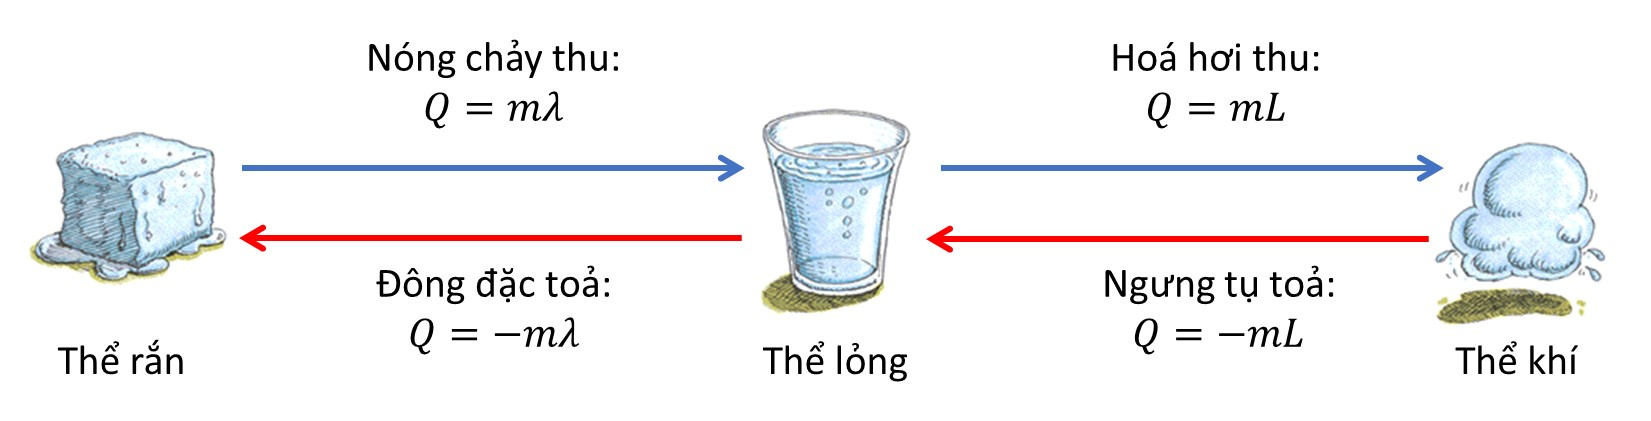
\includegraphics[width=0.8\linewidth]{figs/VN12-Y24-PH-SYL-006-1}
			\captionof{figure}{Sơ đồ chuyển thể}
		\end{center}
	\end{dang}
\begin{vd}
	Rót nước ở nhiệt độ $t_1=\SI{20}{\celsius}$ vào một nhiệt lượng kế. Thả vào trong nhiệt lượng kế một cục nước đá khối lượng $m_2=\SI{0.5}{\kilogram}$ và nhiệt độ $t_2=\SI{-15}{\celsius}$. Biết khối lượng nước đổ vào $m_1=m_2$. Cho biết nhiệt dung riêng của nước $c_1=\SI{4200}{\joule/\left(\kilogram\cdot\kelvin\right)}$, của nước đá $c_2=\SI{2100}{\joule/\left(\kilogram\cdot\kelvin\right)}$ và nhiệt nóng chảy riêng của nước đá $\lambda=\SI{3.4E5}{\joule/\kilogram}$. Bỏ qua sự trao đổi nhiệt với môi trường.
	\begin{enumerate}[label=\alph*)]
		\item Hãy cho biết cục nước đá có tan hết không?
		\item Nếu nước đá tan hết, hãy xác định nhiệt độ của hỗn hợp sau khi cân bằng nhiệt được thiết lập. Nếu nước đá không tan hết, hãy tính khối lượng nước đá đã tan.
	\end{enumerate}
\loigiai{
\begin{enumerate}[label=\alph*)]
	\item Nhiệt lượng nước $\SI{20}{\celsius}$ toả ra để giảm nhiệt độ xuống $\SI{0}{\celsius}$:
	$$Q_1=m_1c_1\left(0-t_1\right)=\left(\SI{0.5}{\kilogram}\right)\cdot\left[\SI{4200}{\joule/\left(\kilogram\cdot\kelvin\right)}\right]\cdot\left(\SI{0}{\celsius}-\SI{20}{\celsius}\right)=\SI{-42000}{\joule}$$
	Nhiệt lượng nước đá cần thu vào để tăng nhiệt độ từ $\SI{-15}{\celsius}$ đến $\SI{0}{\celsius}$ và nóng chảy hoàn toàn:
	$$Q_2=m_2c_2\left(0-t_2\right)+m_2\lambda$$
	$$\Leftrightarrow Q_2=\left(\SI{0.5}{\kilogram}\right)\cdot\left[\SI{2100}{\joule/\left(\kilogram\cdot\kelvin\right)}\right]\cdot\left(\SI{0}{\celsius}+\SI{15}{\celsius}\right)+\left(\SI{0.5}{\kilogram}\right)\cdot\left(\SI{3.4E5}{\joule/\kilogram}\right)=\SI{185750}{\joule}$$
	Vì $\left|Q_1\right|<Q_2$ nên nước đá chỉ tan được một phần.
	\item Vì nước đá chỉ tan một phần nên nhiệt độ của hỗn hợp khi cân bằng nhiệt là $\SI{0}{\celsius}$.\\
	Gọi $m'$ là khối lượng nước đá đã tan.\\
	Nhiệt lượng nước đá cần thu vào để tăng nhiệt độ từ $\SI{-15}{\celsius}$ đến $\SI{0}{\celsius}$ và nóng chảy một phần: $$Q_2'=m_2c_2\left(0-t_2\right)+m'\lambda$$
	Trạng thái cân bằng nhiệt được thiết lập khi tổng nhiệt lượng trao đổi trong hệ bằng 0:
	$$Q_1+Q_2'=0$$
	$$\Leftrightarrow Q_1+m_2c_2\left(0-t_2\right)+m'\lambda=0$$
	\begin{eqnarray*}
		\Rightarrow m'&=&-\dfrac{Q_1+m_2c_2\left(0-t_2\right)}{\lambda}\\
		\Leftrightarrow m'&=&-\dfrac{\SI{-42000}{\joule}+\left(\SI{0.5}{\kilogram}\right)\cdot\left[\SI{2100}{\joule/\left(\kilogram\cdot\kelvin\right)}\right]\cdot\left(\SI{0}{\celsius}+\SI{15}{\celsius}\right)}{\SI{3.4E5}{\joule/\kilogram}}\\
		\Rightarrow m'&\approx&\SI{77.2}{\gram}.
	\end{eqnarray*}
	Vậy khối lượng nước đá đã tan là $\SI{77.2}{\gram}$.
	
	
\end{enumerate}
}
\end{vd}
% ========================================================================
\begin{vd}
	Dẫn $m_1=\SI{100}{\gram}$ hơi nước ở $t_1=\SI{100}{\celsius}$ vào một bình cách nhiệt đựng nước đá ở $t_2=\SI{-4}{\celsius}$. Nước đá bị tan hoàn toàn và nhiệt độ nước trong bình sau khi cân bằng nhiệt là $\SI{10}{\celsius}$. Tìm khối lượng nước đá trong bình. Biết nhiệt nóng chảy riêng của nước đá là $\lambda=\SI{3.4E5}{\joule/\kilogram}$, nhiệt hoá hơi riêng của nước ở $\SI{100}{\celsius}$ là $L=\SI{2.3E6}{\joule/\kilogram}$, nhiệt dung riêng của nước là $c_1=\SI{4200}{\joule/\left(\kilogram\cdot\kelvin\right)}$, nhiệt dung riêng của nước đá là $c_2=\SI{2100}{\joule/\left(\kilogram\cdot\kelvin\right)}$. Bỏ qua sự trao đổi nhiệt với môi trường.
	\loigiai{
	Gọi $\xsi{m}{\left(\kilogram\right)}$ là khối lượng nước đá trong bình.\\
	Nhiệt lượng hơi nước toả ra để ngưng tụ hoàn toàn ở $\SI{100}{\celsius}$ và giảm nhiệt độ từ $\SI{100}{\celsius}$ xuống $\SI{10}{\celsius}$:
	$$Q_1=-m_1L+m_1c_1\left(t_\text{cb}-t_1\right)$$
	$$\Leftrightarrow Q_1=-\left(\SI{0.1}{\kilogram}\right)\cdot\left(\SI{2.3E6}{\joule/\kilogram}\right)+\left(\SI{0.1}{\kilogram}\right)\cdot\left[\SI{4200}{\joule/\left(\kilogram\cdot\kelvin\right)}\right]\cdot\left(\SI{10}{\celsius}-\SI{100}{\celsius}\right)=\SI{-267800}{\joule}$$
	Nhiệt lượng nước đá thu vào để tăng nhiệt độ từ $\SI{-4}{\celsius}$ lên $\SI{0}{\celsius}$, nóng chảy hoàn toàn ở $\SI{0}{\celsius}$ rồi tăng nhiệt độ lên $\SI{10}{\celsius}$:
	$$Q_2=mc_2\left(0-t_2\right)+m\lambda+mc_1\left(t_\text{cb}-0\right)$$
	$$\Leftrightarrow Q_2=m\cdot\left[\SI{2100}{\joule/\left(\kilogram\cdot\kelvin\right)}\right]\cdot\left(\SI{0}{\celsius}+\SI{4}{\celsius}\right)+m\cdot\left(\SI{3.4E5}{\joule/\kilogram}\right)+m\cdot\left[\SI{4200}{\joule/\left(\joule\cdot\kelvin\right)}\right]\cdot\left(\SI{10}{\celsius}-\SI{0}{\celsius}\right)=390400m$$
	Hệ đạt trạng thái cân bằng nhiệt khi tổng nhiệt lượng trao đổi trong hệ bằng 0:
	\begin{eqnarray*}
		&&Q_1+Q_2=0\\
		&\Leftrightarrow& -267800+390400m=0\\
		&\Rightarrow& m\approx\SI{0.686}{\kilogram}.
	\end{eqnarray*}
}
\end{vd}
\subsection{BÀI TẬP TRẮC NGHIỆM}
\setcounter{ex}{0}
\Opensolutionfile{ans}[ans/G12Y24B6TN]		
% ===================================================================
\begin{ex}
Khi vật rắn tinh thể đang nóng chảy thì đại lượng nào của vật sau đây là không thay đổi?	
\choice
{Thể tích}
{Nội năng}
{\True Nhiệt độ}
{Hình dạng}
\loigiai{}
\end{ex}
% ===================================================================
\begin{ex}
	Điều nào sau đây là \textbf{đúng} khi nói về nhiệt nóng chảy riêng?
	\choice
	{Nhiệt nóng chảy riêng của chất rắn là nhiệt lượng cần cung cấp cho vật rắn trong quá trình nóng chảy}
	{Các chất có khối lượng bằng nhau thì có nhiệt độ nóng chảy như nhau}
	{Nhiệt nóng chảy riêng của chất rắn tỉ lệ thuận với khối lượng của vật}
	{\True Đơn vị của nhiệt nóng chảy riêng là $\si{\joule/\kilogram}$}
	\loigiai{}
\end{ex}
% ===================================================================
\begin{ex}
Điều nào sau đây là \textbf{đúng} khi nói về nhiệt nóng chảy riêng của chất rắn?
	\choice
	{Nhiệt nóng chảy riêng của một chất rắn có độ lớn bằng nhiệt lượng cần cung cấp để làm nóng chảy $\SI{1}{\kilogram}$ chất đó ở nhiệt độ nóng chảy}
	{Đơn vị của nhiệt nóng chảy riêng là joule trên kilogram $\left(\si{\joule/\kilogram}\right)$}
	{Các chất khác nhau thì nhiệt nóng chảy riêng của chúng khác nhau}
	{\True Cả A, B, C đều đúng}
	\loigiai{}
\end{ex}
% ===================================================================
\begin{ex}
	Nhiệt nóng chảy riêng của đồng là $\SI{1.8E5}{\joule/\kilogram}$. Câu nào dưới đây là \textbf{đúng}?
	\choice
	{Khối đồng sẽ toả ra nhiệt lượng $\SI{1.8E5}{\joule}$ khi nóng chảy hoàn toàn}
	{\True Mỗi kilogram đồng cần thu nhiệt lượng $\SI{1.8E5}{\joule}$ để hoá lỏng hoàn toàn ở nhiệt độ nóng chảy}
	{Khối đồng cần nhu nhiệt lượng $\SI{1.8E5}{\joule}$ để hoá lỏng}
	{Mỗi kilogram đồng toả ra nhiệt lượng $\SI{1.8E5}{\joule}$ khi hoá lỏng hoàn toàn}
	\loigiai{}
\end{ex}
% ===================================================================
\begin{ex}
	Đơn vị của nhiệt hoá hơi riêng của chất lỏng là
	\choice
	{\True $\si{\joule/\kilogram}$}
	{$\si{\joule\cdot\kilogram}$}
	{$\si{\kilogram/\joule}$}
	{$\si{\joule}$}
	\loigiai{}
\end{ex}
% ===================================================================
\begin{ex}
	Nhiệt hoá hơi riêng của nước là $\SI{2.3E6}{\joule/\kilogram}$. Câu nào dưới đây là \textbf{đúng nhất}?
	\choice
	{Mỗi lượng nước bất kì cần thu một lượng nhiệt $\SI{2.3E6}{\joule}$ để bay hơi hoàn toàn}
	{Mỗi kilogram nước cần thu một lượng nhiệt là $\SI{2.3E6}{\joule}$ để bay hơi hoàn toàn}
	{Mỗi kilogram nước sẽ toả ra một lượng nhiệt là $\SI{2.3E6}{\joule}$ khi bay hơi hoàn toàn ở nhiệt độ sôi}
	{\True Mỗi kilogram nước cần thu một lượng nhiệt là $\SI{2.3E6}{\joule}$ để bay hơi hoàn toàn ở nhiệt độ sôi và áp suất chuẩn}
	\loigiai{}
\end{ex}
% ===================================================================
\begin{ex}
	Biết nhiệt nóng chảy riêng của nước đá là $\SI{3.34E5}{\joule/\kilogram}$. Nhiệt lượng cần cung cấp để làm nóng chảy $\SI{500}{\gram}$ nước đá ở $\SI{0}{\celsius}$ là
	\choice
	{$\SI{7E7}{\joule}$}
	{$\SI{167}{\joule}$}
	{\True $\SI{167}{\kilo\joule}$}
	{$\SI{167e6}{\joule}$}
	\loigiai{	$$Q=m\lambda=\left(\SI{0.5}{\kilogram}\right)\cdot\left(\SI{3.34E5}{\joule/\kilogram}\right)=\SI{167}{\kilo\joule}$$}
\end{ex}
% ===================================================================
\begin{ex}
	Biết nhiệt nóng chảy riêng của nước đá là $\SI{3.34E5}{\joule/\kilogram}$. Người ta cung cấp nhiệt lượng $\SI{5.01E5}{\joule}$ thì có thể làm nóng chảy hoàn toàn bao nhiêu kilogram nước đá?
	\choice
	{$\SI{16.7}{\kilogram}$}
	{\True $\SI{1.5}{\kilogram}$}
	{$\SI{8.35}{\kilogram}$}
	{$\SI{0.668}{\kilogram}$}
	\loigiai{$$m=\dfrac{Q}{\lambda}=\SI{1.5}{\kilogram}$$}
\end{ex}
% ===================================================================
\begin{ex}
	Biết nhiệt dung riêng của nước là $c=\SI{4190}{\joule/\left(\kilogram\cdot\kelvin\right)}$ và nhiệt hoá hơi riêng của nước là $L=\SI{2.26E6}{\joule/\kilogram}$. Để làm cho $\SI{200}{\gram}$ nước ở $\SI{10}{\celsius}$ sôi ở $\SI{100}{\celsius}$ và $\SI{10}{\percent}$ lượng nước này hoá hơi khi sôi thì cần cung cấp một nhiệt lượng \textbf{gần nhất} là
	\choice
	{$\SI{169}{\kilo\joule}$}
	{\True $\SI{121}{\kilo\joule}$}
	{$\SI{189}{\kilo\joule}$}
	{$\SI{212}{\kilo\joule}$}
	\loigiai{	Nhiệt lượng cần cung cấp:
		$$Q=mc\left(100-t\right)+\SI{10}{\percent}mL\approx\SI{121}{\kilo\joule}$$}
\end{ex}
% ===================================================================
\begin{ex}
Cho biết nhiệt dung riêng của nước $\SI{4180}{\joule/\left(\kilogram\cdot\kelvin\right)}$ và nhiệt hoá hơi riêng của nước là $\SI{2.3E6}{\joule/\kilogram}$. Nhiệt lượng cần cung cấp cho $\SI{10}{\kilogram}$ nước ở $\SI{25}{\celsius}$ chuyển thành hơi ở $\SI{100}{\celsius}$ là
	\choice
	{$\SI{18450}{\kilo\joule}$}
	{\True $\SI{26135}{\kilo\joule}$}
	{$\SI{84500}{\kilo\joule}$}
	{$\SI{804500}{\kilo\joule}$}
	\loigiai{	$$Q=mc\Delta t+mL=\SI{26135}{\kilo\joule}$$}
\end{ex}
% ===================================================================
\begin{ex}
	Nước có nhiệt dung riêng $c=\SI{4180}{\joule/\left(\kilogram\cdot\kelvin\right)}$ và nhiệt hoá hơi riêng $L=\SI{2.3E6}{\joule/\kilogram}$. Nhiệt lượng toả ra khi $\SI{4}{\kilogram}$ hơi nước ở $\SI{100}{\celsius}$ ngưng tụ thành nước ở $\SI{22}{\celsius}$ là 
	\choice
	{$\SI{11504160}{\joule}$}
	{$\SI{12504160}{\joule}$}
	{\True $\SI{10504160}{\joule}$}
	{$\SI{13504160}{\joule}$}
	\loigiai{Nhiệt lượng toả ra khi $\SI{4}{\kilogram}$ hơi nước ở $\SI{100}{\celsius}$ ngưng tụ thành nước ở $\SI{22}{\celsius}$ là 
		$$Q=mL+mc\left(t_0-t\right)=\SI{10504160}{\joule}$$}
\end{ex}
% ===================================================================
\begin{ex}
	Người ta có $\SI{5}{\kilogram}$ nước đá ở $\SI{-10}{\celsius}$, cho biết nhiệt dung riêng của nước đá là $\SI{1090}{\joule/\kilogram}$ và nhiệt nóng chảy riêng của nước đá là $\SI{3.4E5}{\joule/\kilogram}$. Nhiệt lượng cần cung cấp để khối đá trên tan hoàn toàn thành nước ở $\SI{0}{\celsius}$ là
	\choice
	{$\SI{4.45}{\kilo\joule}$}
	{\True $\SI{1.8}{\mega\joule}$}
	{$\SI{1.9}{\mega\joule}$}
	{$\SI{1.7}{\mega\joule}$}
	\loigiai{Nhiệt lượng cần cung cấp để khối đá trên tan hoàn toàn thành nước ở $\SI{0}{\celsius}$ là
		$$Q=m\lambda+mc\left(0-t_0\right)=\SI{1804500}{\joule}$$
	}
\end{ex}

% ===================================================================
\begin{ex}
Để xác định nhiệt hóa hơi riêng của nước, người ta làm thí nghiệm sau: đưa $\SI{10}{\gram}$ hơi nước ở nhiệt độ $\SI{100}{\celsius}$ vào một nhiệt lượng kế chứa $\SI{290}{\gram}$ nước ở $\SI{20}{\celsius}$. Nhiệt độ cuối của hệ là $\SI{40}{\celsius}$. Cho biết nhiệt dung của nhiệt lượng kế là  $\SI{46}{\joule/\kelvin}$, nhiệt dung riêng của nước là $\SI{4.18}{\joule/\left(\gram\cdot\kelvin\right)}$. Nhiệt hoá hơi riêng của nước là 
	\choice
	{$\SI{6900}{\joule/\gram}$}
	{\True $\SI{2265.6}{\joule/\gram}$}
	{$\SI{4600}{\joule/\gram}$}
	{$\SI{3200}{\joule/\gram}$}
	\loigiai{Khi hệ cân bằng nhiệt, tổng nhiệt lượng trao đổi trong hệ bằng 0:
		$$-m_\text{hơi}L+m_\text{hơi}c\left(t_\text{cb}-t_\text{hơi}\right)+m_\text{nước}c\left(t_\text{cb}-t_\text{n}\right)=0\Rightarrow L=\SI{2265.6}{\joule/\gram}$$}
\end{ex}
% ===================================================================
\begin{ex}
	Đổ $\SI{100}{\gram}$ nước ở $\SI{40}{\celsius}$ vào một khối nước đá lớn ở $\SI{0}{\celsius}$. Cho nhiệt nóng chảy riêng của nước đá là $\lambda=\SI{80}{cal/\gram\cdot\kelvin}$ và nhiệt dung riêng của nước đá là $c=\SI{1}{cal/\gram\cdot\kelvin}$. Khối lượng nước đá tan chảy là
	\choice
	{$\SI{200}{\gram}$}
	{\True $\SI{50}{\gram}$}
	{$\SI{25}{\gram}$}
	{$\SI{100}{\gram}$}
	\loigiai{	Khối lượng nước đá tan:
		$$m=\dfrac{m_nc_n\Delta t}{\lambda}=\SI{50}{\gram}$$}
\end{ex}
% ===================================================================
\begin{ex}
\immini{Một chậu đựng hỗn hợp nước và nước đá có khối lượng $\SI{10}{\kilogram}$. Chậu để trong phòng và người ta theo dõi nhiệt độ của hỗn hợp. Đồ thị biểu thị sự phụ thuộc nhiệt độ theo thời gian cho ở hình bên. Cho nhiệt dung riêng của nước là $c=\SI{4200}{\joule/\left(\kilogram\cdot\kelvin\right)}$ và nhiệt nóng chảy riêng của nước đá là $\lambda=\SI{3.4E5}{\joule/\kilogram}$. Bỏ qua sự trao đổi nhiệt với chậu. Khối lượng nước đá trong hỗn hợp ban đầu là
	\choice
	{$\SI{0.296}{\kilogram}$}
	{$\SI{1.48}{\kilogram}$}
	{$\SI{0.21}{\kilogram}$}
	{\True $\SI{1.235}{\kilogram}$}
	\loigiai{	$$\dfrac{m_\text{đ}\lambda}{m_\text{hh}c\Delta t}=5\Rightarrow m_\text{đ}\approx\SI{1.235}{\kilogram}$$}}
{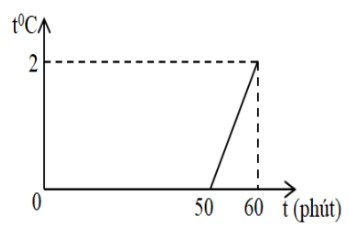
\includegraphics[scale=0.7]{figs/VN12-Y24-PH-SYL-005P-1}

}
\end{ex}
% ===================================================================
\begin{ex}
Người ta thả một cục nước đá khối lượng $\SI{80}{\gram}$ ở $\SI{0}{\celsius}$ vào một cốc nhôm đựng $\SI{0.4}{\kilogram}$ nước ở $\SI{20}{\celsius}$ đặt trong nhiệt lượng kế. Biết khối lượng cốc nhôm là $\SI{0.2}{\kilogram}$. Cho nhiệt nóng chảy riêng của nước đá là $\SI{3.4E5}{\joule/\kilogram}$, nhiệt dung riêng của nhôm là $\SI{880}{\joule/\left(\kilogram\cdot\kelvin\right)}$ và của nước là $\SI{4180}{\joule/\left(\kilogram\cdot\kelvin\right)}$. Bỏ qua sự mất mát nhiệt do truyền ra ngoài. Nhiệt độ của nước khi nước đá đã tan hết là
	\choice
	{\True $\SI{4.5}{\celsius}$}
	{$\SI{5.5}{\celsius}$}
	{$\SI{6.5}{\celsius}$}
	{$\SI{7.5}{\celsius}$}
	\loigiai{		Khi cân bằng nhiệt, tổng nhiệt lượng trao đổi trong hệ bằng 0:
		$$m_\text{đ}\lambda+m_\text{đ}c\left(t_\text{cb}-0\right)+m_\text{n}c\left(t_\text{cb}-t_\text{n}\right)=0\Rightarrow t_\text{cb}\approx\SI{4.47}{\celsius}$$}
\end{ex}
% ===================================================================
\begin{ex}
	Lấy $\SI{0.01}{\kilogram}$ hơi nước ở $\SI{100}{\celsius}$ cho ngưng tụ trong bình nhiệt lượng kế chứa $\SI{0.2}{\kilogram}$ nước ở $\SI{9.5}{\celsius}$; nhiệt độ cuối cùng của nước là $\SI{40}{\celsius}$. Cho nhiệt dung riêng của nước là $c=\SI{4180}{\joule/\left(\kilogram\cdot\kelvin\right)}$. Nhiệt hoá hơi riêng của nước là
	\choice
	{$\SI{3.1e6}{\joule/\kilogram}$}
	{$\SI{2.8e6}{\joule/\kilogram}$}
	{\True $\SI{2.3e6}{\joule/\kilogram}$}
	{$\SI{1.4e6}{\joule/\kilogram}$}
	\loigiai{Áp dụng phương trình cân bằng nhiệt:
		$$m_1L+m_1c\left(100-t_\text{cb}\right)=m_2c\left(t_\text{cb}-t_2\right)$$
		$$\Leftrightarrow 0,01L+0,01\cdot4180\cdot\left(100-40\right)=0,2\cdot4180\cdot\left(40-9,5\right)\Rightarrow L=\SI{2.299E6}{\joule/\kilogram}$$
	}
\end{ex}
% ===================================================================
\begin{ex}
	Một khối nước đá có khối lượng $\SI{0.2}{\kilogram}$ ở $\SI{-20}{\celsius}$. Cho biết nhiệt dung riêng của nước đá là $\SI{2.09E3}{\joule/\left(\kilogram\cdot\kelvin\right)}$, nhiệt nóng chảy riêng của nước đá là $\SI{3.4E5}{\joule/\kilogram}$, nhiệt dung riêng của nước là $\SI{4.18E3}{\joule/\left(\kilogram\cdot\kelvin\right)}$, nhiệt hoá hơi riêng của nước là $\SI{2.3E6}{\joule/\kilogram}$. Nhiệt lượng cần cung cấp cho khối nước đá để nó hoá hơi hoàn toàn ở $\SI{100}{\celsius}$ là
	\choice
	{$Q=\SI{205.96}{\kilo\joule}$}
	{\True $Q=\SI{619.96}{\kilo\joule}$}
	{$Q=\SI{159.96}{\kilo\joule}$}
	{$Q=\SI{460}{\kilo\joule}$}
	\loigiai{Nhiệt lượng cần cung cấp cho khối nước đá để nó hoá hơi hoàn toàn ở $\SI{100}{\celsius}$ là
		$$Q=mc_\text{đ}\left(0-t_\text{đ}\right)+m\lambda+mc\left(t_s-0\right)+mL=\SI{619.96}{\kilo\joule}$$}
\end{ex}
% ===================================================================
\begin{ex}
	Cần cung cấp một nhiệt lượng bằng bao nhiêu để làm cho $m=\SI{200}{\gram}$ nước lấy ở $t_1=\SI{10}{\celsius}$ sôi ở $t_2=\SI{100}{\celsius}$ và $\SI{10}{\percent}$ khối lượng của nó đã hoá hơi khi sôi. Biết nhiệt dung riêng của nước là $c=\SI{4190}{\joule/\left(\kilogram\cdot\kelvin\right)}$ và nhiệt hoá hơi riêng của nước là $L=\SI{2.26E6}{\joule/\kilogram}$. Chọn đáp án \textbf{đúng}.
	\choice
	{$\SI{129525}{\joule}$}
	{$\SI{110610}{\joule}$}
	{\True $\SI{120620}{\joule}$}
	{$\SI{130610}{\joule}$}
	\loigiai{$$Q=mc\Delta t+\SI{10}{\percent}mL=\SI{120620}{\joule}$$}
\end{ex}
% ===================================================================
\begin{ex}
	Lấy $\SI{0.01}{\kilogram}$ cho ngưng tụ trong bình nhiệt lượng kế chứa $\SI{0.2}{\kilogram}$ nước ở $\SI{9.5}{\celsius}$. Nhiệt độ cuối cùng đo được là $\SI{40}{\celsius}$. Cho nhiệt dung riêng của nước là $c=\SI{4180}{\joule/\left(\kilogram\cdot\kelvin\right)}$. Nhiệt hoá hơi riêng của nước là
	\choice
	{$\SI{6.9E6}{\joule/\kilogram}$}
	{\True $\SI{2.3E6}{\joule/\kilogram}$}
	{$\SI{4.6E6}{\joule/\kilogram}$}
	{$\SI{3.2E6}{\joule/\kilogram}$}
	\loigiai{Khi hệ cân bằng nhiệt, tổng nhiệt lượng trao đổi trong hệ bằng 0:
		$$-m_\text{hơi}L+m_\text{hơi}c\left(t_\text{cb}-t_\text{hơi}\right)+m_\text{nước}c\left(t_\text{cb}-t_\text{nước}\right)=0\Rightarrow L\approx\SI{2.3E6}{\joule/\kilogram}$$
	}
\end{ex}
% ===================================================================
\begin{ex}
	Để xác định nhiệt nóng chảy riêng của thiếc, người ta đổ $\SI{350}{\gram}$ thiếc nóng chảy ở nhiệt độ $\SI{232}{\celsius}$ vào $\SI{330}{\gram}$ nước ở $\SI{7}{\celsius}$ đựng trong một nhiệt lượng kế có nhiệt dung bằng $\SI{100}{\joule/\kelvin}$. Sau khi cân bằng nhiệt, nhiệt độ của nước trong nhiệt lượng kế là $\SI{32}{\celsius}$. Biết nhiệt dung riêng của nước và thiếc rắn lần lượt là $\SI{4.2}{\joule/\left(\gram\cdot\kelvin\right)}$, $\SI{0.23}{\joule/\left(\gram\cdot\kelvin\right)}$. Nhiệt nóng chảy riêng của thiếc \textbf{gần với giá trị nào nhất} sau đây?
	\choice
	{\True $\SI{60}{\joule/\gram}$}
	{$\SI{73}{\joule/\gram}$}
	{$\SI{89}{\joule/\gram}$}
	{$\SI{96}{\joule/\gram}$}
	\loigiai{Khi hệ cân bằng nhiệt, tổng nhiệt lượng trao đổi trong hệ bằng 0:
		$$-m_\text{th}\lambda+m_\text{th}c_\text{th}\left(t_\text{cb}-t_\text{th}\right)+\left(m_\text{n}c_\text{n}+c_\text{nlk}\right)\cdot\left(t_\text{cb}-t_\text{n}\right)=0$$
		$$\Rightarrow \lambda=\dfrac{m_\text{th}c_\text{th}\left(t_\text{cb}-t_\text{th}\right)+\left(m_\text{n}c_\text{n}+c_\text{nlk}\right)\cdot\left(t_\text{cb}-t_\text{n}\right)}{m_\text{th}}\approx\SI{60.1}{\joule/\gram}$$
	}
\end{ex}

% ===================================================================
\begin{ex}
Một viên đạn chì phải có tốc độ tối thiểu bằng bao nhiêu để khi nó va chạm vào vật cứng thì nóng chảy hoàn toàn? Cho rằng, $\SI{80}{\percent}$ động năng của viên đạn chuyển thành nội năng của nó khi va chạm; nhiệt độ của viên đạn trước khi va chạm là $\SI{127}{\celsius}$. Cho biết nhiệt dung riêng của chì là $\SI{130}{\joule/\left(\kilogram\cdot\kelvin\right)}$; nhiệt độ nóng chảy của chì là $\SI{327}{\celsius}$ và nhiệt nóng chảy riêng của chì là $\lambda=\SI{25}{\kilo\joule/\kilogram}$.
	\choice
	{\True $\SI{357}{\meter/\second}$}
	{$\SI{324}{\meter/\second}$}
	{$\SI{352}{\meter/\second}$}
	{$\SI{457}{\meter/\second}$}
	\loigiai{	Nhiệt lượng cần thiết để viên đạn tăng nhiệt độ từ $\SI{127}{\celsius}$ lên $\SI{327}{\celsius}$ và nóng chảy hoàn toàn:
		$$Q=mc\left(t-t_0\right)+m\lambda=51000m$$
		Áp dụng định lý động năng:
		$$0-\dfrac{1}{2}mv^2_0=-\dfrac{Q}{0.8}$$
		$$\Leftrightarrow \dfrac{1}{2}mv^2_0=\dfrac{51000m}{0.8}\Rightarrow v_0\approx\SI{357}{\meter/\second}$$}
\end{ex}
% ===================================================================
\begin{ex}
	Trong một nhiệt lượng kế bằng nhôm khối lượng $m_\text{nl}=\SI{300}{\gram}$ có một cục nước đá nặng $m_\text{nđ}\left(\si{\gram}\right)$. Nhiệt độ của nhiệt lượng kế và nước đá là $t_1=\SI{-5}{\celsius}$. Sau đó người ta cho $m_\text{hn}\left(\si{\gram}\right)$ hơi nước ở $t_2=\SI{100}{\celsius}$ vào nhiệt lượng kế và khi đã cân bằng nhiệt độ thì nhiệt độ của nhiệt lượng kế là $t_3=\SI{25}{\celsius}$. Lúc đó, trong nhiệt lượng kế có $\SI{500}{\gram}$ nước. Cho biết nhiệt hoá hơi riêng của nước là $L=\SI{2.26E3}{\joule/\gram}$, nhiệt nóng chảy của nước đá $\lambda=\SI{334}{\joule/\gram}$, nhiệt dung riêng của nhôm, của nước đá và của nước lần lượt là $c_\text{nl}=\SI{0.88}{\joule/\gram\cdot\kelvin}$, $c_\text{nđ}=\SI{2.09}{\joule/\gram\cdot\kelvin}$ và $c_\text{n}=\SI{4.19}{\joule/\gram\cdot\kelvin}$. Giá trị của $\left(m_\text{nđ}-3m_\text{hn}\right)$ \textbf{gần với giá trị nào nhất} sau đây?
	\choice
	{$\SI{226}{\gram}$}
	{$\SI{253}{\gram}$}
	{$\SI{269}{\gram}$}
	{\True $\SI{192}{\gram}$}
	\loigiai{Ta có:
		\begin{equation}
			\label{eq:6P-1}
			m_\text{nđ}+m_\text{hn}=\SI{500}{\gram}
		\end{equation}
		Khi có cân bằng nhiệt, tổng nhiệt lượng trao đổi trong hệ bằng 0:
		$$-m_\text{hn}L+m_\text{hn}c\left(t_3-t_2\right)+m_\text{nđ}c_\text{nđ}\left(0-t_1\right)+m_\text{nđ}\lambda+m_\text{nl}c_\text{nl}\left(t_3-t_1\right)+m_\text{nđ}c_\text{n}\left(t_3-0\right)=0$$
		\begin{equation}
			\label{eq:6P-2}
			-2574.25m_\text{hn}+449,2m_\text{nđ}=-7920
		\end{equation}
		Từ (\ref{eq:6P-1}) và (\ref{eq:6P-2}), suy ra:
		$$\begin{cases}
			m_\text{hn}=\SI{76.9}{\gram}\\
			m_\text{nđ}=\SI{423.1}{\gram}
		\end{cases}$$
		Như vậy, $\left(m_\text{nđ}-3m_\text{hn}\right)=\SI{192.4}{\gram}$
	}
\end{ex}
\Closesolutionfile{ans}
	\subsection{TRẮC NGHIỆM ĐÚNG/SAI}
	\setcounter{ex}{0}
% =======================================================================
\begin{ex}
		Bảng dưới đây là nhiệt độ nóng chảy của một số chất.
	\begin{center}
		\begin{tabular}{|C{5cm}|C{1.25cm}|C{1.25cm}|C{1.25cm}|C{1.25cm}|C{1.25cm}|C{1.25cm}|C{1.25cm}|}
			\hline
			\thead{Chất} & Nhôm & Nước đá & Rượu & Sắt & Đồng & Thuỷ ngân & Muối ăn\\
			\hline
			\thead{Nhiệt độ nóng chảy\\ $\left(\si{\celsius}\right)$}& 660 & 0 & -117 & 1535 & 1083 & -39 & 801\\
			\hline
		\end{tabular}
	\end{center}
	\begin{enumerate}[label=\alph*)]
		\item Chất có nhiệt độ nóng chảy cao nhất là đồng.
		\item Chất có nhiệt độ nóng chảy thấp nhất là thuỷ ngân.
		\item Có thể dùng nhiệt kế rượu để đo nhiệt độ thấp tới $\SI{-50}{\celsius}$.
		\item Có thể dùng nhiệt kế thuỷ ngân để đo nhiệt độ thấp tới $\SI{-50}{\celsius}$.
	\end{enumerate}
	\loigiai{	\begin{enumerate}[label=\alph*)]
			\item Sai.
			\item Sai. Chất có nhiệt độ nóng chảy thấp nhất là rượu.
			\item Đúng.
			\item Sai. Thuỷ ngân đã đông đặc ở $\SI{-39}{\celsius}$.
	\end{enumerate}}
	\end{ex}
% =======================================================================
\begin{ex}
	\immini{
		Nếu đặt tô kem lỏng vào giữa chậu nước đá, kem sẽ chỉ lạnh đi nhưng rất khó có thể đông đặc lại. Tuy nhiên, nếu em cho thêm một ít muối vào chậu nước đá này thì kem lỏng có thể đông đặc lại thành đá như hình minh hoạ bên dưới rất nhanh.
		\begin{enumerate}[label=\alph*)]
			\item Kem lạnh đi do nhận nhiệt từ nước đá.
			\item Khi cân bằng nhiệt diễn ra, nếu trong đá có lẫn nước thì nhiệt độ của hỗn hợp nước và nước đá là $\SI{0}{\celsius}$.
			\item Nước muối thấm qua tô vào kem và làm tăng nhiệt độ đông đặc của kem (kem đông đặc ở nhiệt độ trên $\SI{0}{\celsius}$).
			\item Nhiệt độ đông đặc của nước trong thau sau khi cho muối vào bị giảm.
		\end{enumerate}
}{
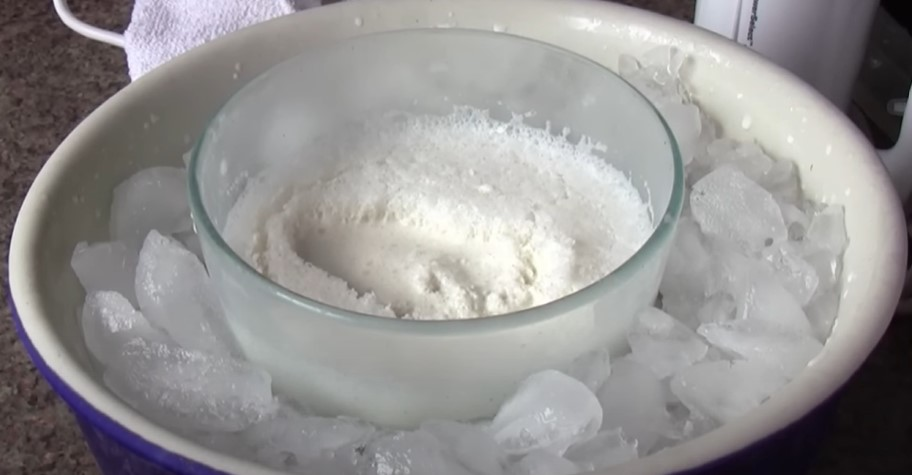
\includegraphics[scale=0.3]{figs/VN12-Y24-PH-SYL-006P-1}
%\caption{Kem lỏng nhanh chóng đông thành đá khi cho muối vào thau nước đá}
}
\loigiai{\begin{enumerate}[label=\alph*)]
		\item Sai. Kem lạnh đi là do kem toả nhiệt cho thau đá.
		\item Đúng.
		\item Sai. Nước muối không thể thấm qua tô do sự liên kết của các phân tử chất rắn rất chặt chẽ. Ở điều kiện tiêu chuẩn, nhiệt độ đông đặc của nước là $\SI{0}{\celsius}$.
		\item Đúng. Nhiệt độ đông đặc của nước trong thau sau khi cho muối vào bị giảm là do sự phân li của các ion trong phân tử muối ăn làm ảnh hưởng đến liên kết hydrogen của các phân tử nước. Do đó, các phân tử nước khó liên kết lại với nhau thành thể rắn hơn
\end{enumerate}}
	\end{ex}
\subsection{BÀI TẬP TỰ LUẬN}
\setcounter{ex}{0}
% ========================================================================
\begin{ex}

	Trên hình vẽ dưới đây biểu diễn đồ thị nhiệt độ của một chất theo thời gian trong quá trình đông đặc. Dựa vào đồ thị, em hãy trả lời các câu hỏi sau:
	\begin{center}
		\begin{tikzpicture}  
			\begin{axis}[  ultra thick,
				xmin=0,  
				xmax=28,  
				xtick={0,5,...,25},
				ytick={-40,-30,...,30},
				minor x tick num=1,
				minor y tick num=4,
				ymin=-48,  
				ymax=35, 
				samples=300,
				axis lines=center, 
				grid style={step=1, line width =0.4pt, color=gray!30!white},
				grid=both,
				major grid style={line width=0.8pt,gray!60!white},
				xlabel=$\xsi{t}{\left(\si{\text{phút}}\right)}$, 		ylabel=$\xsi{t}{\celsius}$,
				every axis y label/.style={at=(current axis.above origin),anchor=south},  
				every axis x label/.style={at=(current axis.right of origin),anchor=west},  ]
				\draw [ultra thick, red] (axis cs: 0,12) --(axis cs: 7.5,-40)--(axis cs: 25,-40)--(axis cs: 25.72,-45); 
				\filldraw[black] (axis cs:0,12) circle (1pt) node[right] {A};
				\filldraw[black] (axis cs:7.5,-40) circle (1pt) node[below] {B}; 
				\filldraw[black] (axis cs:25,-40) circle (1pt) node[below left] {C}; 
			\end{axis}
			\node[left] at (-0.1,3.2) {0};  
		\end{tikzpicture}
	\end{center}
	\begin{enumerate}[label=\alph*)]
		\item Các đoạn AB và BC biểu diễn quá trình gì?
		\item Nhiệt độ ban đầu của chất này là bao nhiêu?
		\item Nhiệt độ đông đặc của chất này là bao nhiêu?
		\item Quá trình làm nguội và đông đặc diễn ra bao lâu?
	\end{enumerate}

\loigiai{
	\begin{enumerate}[label=\alph*)]
		\item AB là quá trình chất này giảm nhiệt độ (quá trình làm nguội), BC là quá trình chất này đông đặc.
		\item Nhiệt độ ban đầu của chất này là $\SI{12}{\celsius}$.
		\item Nhiệt độ đông đặc của chất này là $\SI{-40}{\celsius}$.
		\item Qúa trình làm nguội diễn ra trong $\SI{7.5}{\text{phút}}$, quá trình đông đặc diễn ra trong $\SI{17.5}{\text{phút}}$.
	\end{enumerate}}
	\end{ex}
% ========================================================================
\begin{ex}
	Vận động viên chạy Marathon mất rất nhiều nước trong khi thi đấu. Các vận động viên thường chỉ có thể chuyển hoá khoảng $\SI{20}{\percent}$ năng lượng hoá học dự trữ trong cơ thể thành năng lượng dùng cho các hoạt động của cơ thể, đặc biệt là hoạt động chạy. Phần năng lượng còn lại chuyển thành nhiệt thải ra ngoài nhờ sự bay hơi của nước qua hô hấp và da để giữ nhiệt độ cơ thể ổn định. Nếu vận động viên dùng hết $\SI{11000}{\kilo\joule}$ trong cuộc thi thì có khoảng bao nhiêu lít nước đã thoát ra khỏi cơ thể? Coi nhiệt độ cơ thể của vận động viên hoàn toàn không đổi và nhiệt hoá hơi riêng của nước trong cơ thể vận động viên là $\SI{2.45E6}{\joule/\kilogram}$.
	\loigiai{
		Lượng hơi nước thoát ra khỏi cơ thể vận động viên:
		$$m=\dfrac{\SI{80}{\percent}\cdot W}{L}\approx\SI{3.59}{\kilogram}$$
	}
	\end{ex}
% ========================================================================
\begin{ex}
	Để hàn các linh kiện bị đứt trong mạch điện tử, người thợ sửa chữa thường sử dụng mỏ hàn điện để làm nóng chảy dây thiếc hàn. Biết rằng loại thiếc hàn sử dụng là hỗn hợp của thiếc và chì với tỉ lệ khối lượng $63:37$, khối lượng một cuộn dây thiếc hàn là $\SI{50}{\gram}$. Biết thiếc và chì có nhiệt nóng chảy riêng lần lượt là $\SI{0.61E5}{\joule/\kilogram}$ và $\SI{0.25E5}{\joule/\kilogram}$. Nhiệt lượng mỏ hàn cần cung cấp để làm nóng chảy hết một cuộn dây thiếc hàn ở nhiệt độ nóng chảy bằng bao nhiêu?
	\loigiai{
		$$\dfrac{m_t}{m_c}=\dfrac{63}{37}\xrightarrow{m_t+m_c=\SI{50}{\gram}}\begin{cases}
			m_t=\SI{31.5}{\gram}\\
			m_c=\SI{18.5}{\gram}
		\end{cases}$$
		Nhiệt lượng mỏ hàn cần cung cấp để làm nóng chảy hết một cuộn dây thiếc hàn ở nhiệt độ nóng chảy:
		$$Q=m_t\lambda_t+m_c\lambda_c=\SI{2384}{\joule}$$
	}
\end{ex}
% ========================================================================
\begin{ex}
Một ấm đun nước có công suất $\SI{500}{\watt}$ chứa $\SI{300}{\gram}$ nước. Cho nhiệt hoá hơi riêng của nước là $\SI{2E6}{\joule/\kilogram}$. Sau khi đun nước trong ấm đến nhiệt độ sôi, người ta để ấm tiếp tục đun nước sôi trong 2 phút. Bỏ qua sự mất mát nhiệt. Khối lượng nước còn lại trong ấm bằng bao nhiêu?
\loigiai{
	Lượng nước hoá hơi:
	$$m'=\dfrac{\calP t}{L}=\SI{0.03}{\kilogram}=\SI{30}{\gram}$$
	Lượng nước còn lại trong ấm là
	$$m=M-m'=\SI{270}{\gram}$$
}
\end{ex}
% ========================================================================
\begin{ex}
		Người ta bỏ một cục nước đá khối lượng $m_1=\SI{100}{\gram}$ vào một nhiệt lượng kế bằng đồng có khối lượng $m_2=\SI{125}{\gram}$, thì nhiệt độ của nhiệt lượng kế và nước đá là $t_1=\SI{-20}{\celsius}$. Tính nhiệt lượng cần thiết để làm tan được một nửa lượng nước đá trên. Cho nhiệt dung riêng của đồng là $c_2=\SI{380}{\joule/\kilogram\cdot\kelvin}$, của nước đá là $c_1=\SI{2100}{\joule/\kilogram\cdot\kelvin}$, nhiệt nóng chảy riêng của nước đá là $\SI{3.34E5}{\joule/\kilogram}$.
	\loigiai{
	Nhiệt lượng cần cung cấp cho nhiệt lượng kế để nước đá tan được 1 nửa:
	$$Q=\left(m_1c_1+m_2c_2\right)\cdot\left(0-t_1\right)+\dfrac{m_1}{2}\lambda=\SI{21850}{\joule}.$$	
	}
\end{ex}
% ========================================================================
\begin{ex}
Người ta trộn $m_1=\SI{500}{\gram}$ nước đá với $m_2=\SI{500}{\gram}$ nước ở cùng nhiệt độ $t_1=\SI{0}{\celsius}$ vào một xô nước ở nhiệt độ $\SI{50}{\celsius}$. Khối lượng tổng cộng của chúng là $m=\SI{2}{\kilogram}$. Tính nhiệt độ của xô nước khi có cân bằng nhiệt. Cho nhiệt dung riêng của nước $c=\SI{4200}{\joule/\left(\kilogram\cdot\kelvin\right)}$, nhiệt nóng chảy riêng của nước đá $\lambda=\SI{3.4E5}{\joule/\kilogram}$. Bỏ qua khối lượng và sự thu nhiệt của xô.
\loigiai{
	Khi cân bằng nhiệt, tổng nhiệt lượng trao đổi trong hệ bằng 0:
	$$m_1\lambda+\left(m_1+m_2\right)c\left(t_\text{cb}-0\right)+\left(m-m_1-m_2\right)c\left(t_\text{cb}-t_0\right)=0$$
	$$\Leftrightarrow 0,5\cdot\SI{3.4E5}{}+1\cdot4200\cdot t_\text{cb}+1\cdot4200\left(t_\text{cb}-50\right)=0\Rightarrow t_\text{cb}\approx\SI{4.76}{\celsius}$$
}
\end{ex}
% ========================================================================
\begin{ex}
Bỏ $\SI{20}{\gram}$ tuyết có lẫn nước ở $\SI{0}{\celsius}$ vào nhiệt lượng kế chứa $\SI{250}{\gram}$ nước ở $\SI{15}{\celsius}$. Khi cân bằng nhiệt, nhiệt độ của nhiệt lượng kế giảm $\SI{5}{\celsius}$. Hỏi khối lượng nước lẫn trong tuyết là bao nhiêu? Biết nhiệt nóng chảy riêng của nước đá là $\lambda=\SI{3.4E5}{\joule/\kilogram}$, nhiệt dung riêng của nước $c=\SI{4200}{\joule/\left(\kilogram\cdot\kelvin\right)}$. Bỏ qua nhiệt dung của nhiệt lượng kế.
\loigiai{
	Gọi $m_1$, $m_2$ lần lượt là khối lượng của nước và đá trong tuyết.\\
	Ta có:
	\begin{equation*}
		m_1+m_2=\SI{0.02}{\kilogram}
	\end{equation*}
	Khi cân bằng nhiệt, tổng nhiệt lượng trao đổi trong hệ bằng 0:
	$$m_2\lambda+\left(m_1+m_2\right)c\left(t_\text{cb}-0\right)+m_\text{n}c\left(t_\text{cb}-t_\text{n}\right)=0$$
	$$\Rightarrow m_2\approx\SI{0.013}{\kilogram}=\SI{13}{\gram}$$
	Như vậy, khối lượng nước lẫn trong tuyết là $m_1\approx\SI{7}{\gram}$
}
\end{ex}
% ========================================================================
\begin{ex}
Trong ruột cục nước đá lớn ở $\SI{0}{\celsius}$ có một cái hốc với thể tích bằng $V=\SI{160}{\centi\meter^3}$. Người ta rót vào hốc đó $\SI{60}{\gram}$ ở nhiệt độ $\SI{75}{\celsius}$. Cho khối lượng riêng của nước $D_1=\SI{1}{\gram/\centi\meter^3}$ và của nước đá $D_2=\SI{0.9}{\gram/\centi\meter^3}$, nhiệt dung riêng của nước là $c=\SI{4200}{\joule/\left(\kilogram\cdot\kelvin\right)}$ và để làm nóng chảy hoàn toàn $\SI{1}{\kilogram}$ nước đá ở nhiệt độ nóng chảy cần cung cấp cho khối nước đá này một nhiệt lượng $\SI{3.36E5}{\joule}$. Hỏi khi nước nguội hẳnn thì thể tích hốc rỗng còn lại là bao nhiêu $\si{\centi\meter^3}$?
\loigiai{
	Nhiệt lượng do nước toả ra để giảm nhiệt độ từ $\SI{75}{\celsius}$ về $\SI{0}{\celsius}$:
	$$Q_\text{toả}=m_\text{n}c\left(0-t_\text{n}\right)=\SI{18900}{\joule}$$
	Thể tích nước rót vào hốc:
	$$V_n=\dfrac{m_n}{D_1}=\SI{60}{\centi\meter^3}$$
	Khối lượng nước đá tan:
	$$m_\text{đá}=\dfrac{Q_\text{thu}}{\lambda}=\dfrac{Q_\text{toả}}{\lambda}=\SI{56.25}{\gram}$$
	Thể tích nước đá bị tan là
	$$V_\text{đ}=\dfrac{m_\text{đ}}{D_2}=\SI{62.5}{\centi\meter^3}$$
	Thể tích nước tạo thành do đá tan:
	$$V_1=\dfrac{m_\text{đ}}{D_1}=\SI{56.25}{\centi\meter^3}$$
	Thể tích phần rỗng còn lại:
	$$V+V_\text{đ}-V_1-V_\text{n}=\SI{106.25}{\centi\meter^3}$$
}
\end{ex}
% ========================================================================
\begin{ex}
Dẫn hơi nước ở $\SI{100}{\celsius}$ vào một bình nước đang có nhiệt độ $\SI{20}{\celsius}$ dưới áp suất bình thường.
\begin{enumerate}[label=\alph*)]
	\item Khối lượng nước trong bình tăng lên bao nhiêu lần khi nhiệt độ của nó đạt tới $\SI{100}{\celsius}$.
	\item Khi nhiệt độ của nước đạt tới $\SI{100}{\celsius}$, nếu tiếp tục dẫn hơi nước ở $\SI{100}{\celsius}$ vào bình thì có thể làm cho nước trong bình có thể sôi được không?
\end{enumerate}
Cho:
\begin{itemize}
	\item nhiệt dung riêng của nước $c=\SI{4200}{\joule/\left(\kilogram\cdot\kelvin\right)}$;
	\item nhiệt hoá hơi riêng của nước $L=\SI{2.3E6}{\joule/\kilogram}$.
\end{itemize}
	\loigiai{
	\begin{enumerate}[label=\alph*)]
		\item Gọi $m$ là khối lượng hơi nước ngưng tụ và $M$ là khối lượng nước có sẵn trong bình.\\
		Khi có cân bằng nhiệt, tổng nhiệt lượng trao đổi trong hệ bằng 0:
		$$-mL+Mc\left(100-t_0\right)=0\Rightarrow m=0,146M.$$
		$$\Rightarrow \dfrac{m+M}{M}=1,146.$$
		\item Nước không thể sôi vì hệ đã đạt trạng thái cân bằng nhiệt ở $\SI{100}{\celsius}$ nên không thể nhận thêm nhiệt lượng để hoá thành hơi.
	\end{enumerate}
	}
\end{ex}
% ========================================================================
\begin{ex}
	Người ta dẫn hơi nước ở $\SI{100}{\celsius}$ vào một nhiệt lượng kế chứa $\SI{100}{\gram}$ nước đá ở $\SI{0}{\celsius}$. Sau khi nước đá tan hết, khối lượng nước trong nhiệt lượng kế là bao nhiêu? Cho nhiệt nóng chảy riêng của nước đá là $\lambda=\SI{3.4E5}{\joule/\kilogram}$; nhiệt hoá hơi riêng của nước $L=\SI{2.26E6}{\joule/\kilogram}$; nhiệt dung riêng của nước $c=\SI{4200}{\joule/\left(\kilogram\cdot\kelvin\right)}$ và bỏ qua nhiệt dung của nhiệt lượng kế.
	\loigiai{
		Gọi $m$ là khối lượng hơi nước ngưng tụ thành nước và $m_\text{đ}$ là khối lượng nước đá nóng chảy.\\
		Khi có cân bằng nhiệt, tổng nhiệt lượng trao đổi của hệ bằng 0:
		$$m_\text{đ}\lambda-mL+mc\left(0-100\right)=0\Rightarrow m=\SI{0.0127}{\kilogram}.$$
		Lượng nước tăng thêm trong bình:
		$$m_\text{n}=m_\text{đ}+m=\SI{112.7}{\gram}.$$
	}
\end{ex}
% ========================================================================
\begin{ex}
		Người ta đổ $\xsi{m_1}{\left(\kilogram\right)}$ nước ở nhiệt độ $t_1=\SI{60}{\celsius}$ vào $\xsi{m_2}{\left(\kilogram\right)}$ nước đá ở nhiệt độ $t_2=\SI{-5}{\celsius}$. Khi có cân bằng nhiệt, lượng nước thu được là $m=\SI{50}{\kilogram}$ có nhiệt độ $t=\SI{25}{\celsius}$. Xác định $m_1$ và $m_2$. Cho nhiệt dung riêng của nước và nước đá lần lượt là $c_1=\SI{4200}{\joule/\left(\kilogram\cdot\kelvin\right)}$, $c_2=\SI{2100}{\kilogram/\left(\kilogram\cdot\kelvin\right)}$, nhiệt nóng chảy riêng của nước đá $\lambda=\SI{3.4E5}{\joule/\kilogram}$.
	\loigiai{
	Ta có:
	\begin{equation}
		\label{eq:6P-1}
		m_1+m_2=\SI{50}{\kilogram}
	\end{equation}	
	Khi cân bằng nhiệt xảy ra, tổng nhiệt lượng trao đổi trong hệ bằng 0:
	$$m_1c_1\left(t_\text{cb}-t_1\right)+m_2c_2\left(0-t_2\right)+m_2\lambda+m_2c_1\left(t_\text{cb}-t_1\right)=0.$$
	\begin{equation}
		\label{eq:6P-2}
		-147000m_1+455500m_2=0
	\end{equation}
	Từ (\ref{eq:6P-1}) và (\ref{eq:6P-2}), suy ra:
	\begin{equation*}
		\begin{cases}
			m_1=\SI{37.8}{\kilogram}\\
			m_2=\SI{12.2}{\kilogram}
		\end{cases}
	\end{equation*}
	}
\end{ex}
% ========================================================================
\begin{ex}
Cho $\SI{100}{\gram}$ nước đá ở nhiệt độ $t_1=\SI{0}{\celsius}$ vào $\SI{300}{\gram}$ nước ở nhiệt độ $t_2=\SI{20}{\celsius}$. Hỏi nước đá có tan hết không? Nếu không, em hãy tính khối lượng nước đá còn lại.\\
Cho nhiệt nóng chảy riêng của nước đá là $\lambda=\SI{3.4E5}{\joule/\kilogram}$ và nhiệt dung riêng của nước là $c=\SI{4200}{\joule/\left(\kilogram\cdot\kelvin\right)}$.
	\loigiai{
	Nhiệt lượng nước đá thu vào để nóng chảy hoàn toàn
	$$Q_\text{thu}=m_\text{đ}\lambda=\SI{3.4E4}{\joule}.$$
	Nhiệt lượng nước toả ra để giảm nhiệt độ từ $\SI{20}{\celsius}$ xuống $\SI{0}{\celsius}$:
	$$Q_\text{toả}=m_\text{n}c\left(t_\text{n}-0\right)=\SI{2.52E4}{\joule}.$$
	Vì $Q_\text{thu}>Q_\text{toả}$ nên nước đá không tan hết.\\
	Gọi $m$ là khối lượng nước đá tan.\\
	Do nước đá không tan hết nên nhiệt độ của hệ khi cân bằng nhiệt là $\SI{0}{\celsius}$.\\
	Khối lượng nước đá tan:
	$$m=\dfrac{Q_\text{toả}}{\lambda}\approx\SI{0.07412}{\kilogram}\approx\SI{74.12}{\gram}.$$
	Vậy: khối lượng nước đá còn lại là xấp xỉ $\SI{25.88}{\gram}$.
	}
\end{ex}
% ========================================================================
\begin{ex}
\begin{enumerate}[label=\alph*)]
	\item Tính nhiệt lượng do $\SI{500}{\gram}$ nước ở $\SI{30}{\celsius}$ toả ra khi nhiệt độ của nó hạ xuống $\SI{0}{\celsius}$.
	\item Để biến lượng nước trên thành nước đá, người ta bỏ vào nước trên một khối nước đá ở nhiệt độ $\SI{-10}{\celsius}$. Tính khối lượng nước đá tối thiểu cần dùng.
\end{enumerate}
Cho:
\begin{itemize}
	\item nhiệt dung riêng của nước $c_\text{n}=\SI{4200}{\joule/\left(\kilogram\cdot\kelvin\right)}$;
	\item nhiệt dung riêng của nước đá $c_\text{đ}=\SI{2000}{\joule/\left(\kilogram\cdot\kelvin\right)}$;
	\item nhiệt nóng chảy riêng của nước đá $\lambda=\SI{3.4E5}{\joule/\kilogram}$.
\end{itemize}
	\loigiai{
		\begin{enumerate}[label=\alph*)]
			\item Nhiệt lượng do $\SI{500}{\gram}$ nước đá toả ra để hạ nhiệt độ từ $\SI{30}{\celsius}$ xuống $\SI{0}{\celsius}$:
			$$Q_1=m_\text{n}c_\text{n}\left(t_\text{n}-0\right)=\SI{63}{\kilo\joule}.$$
			\item Nhiệt lượng tối thiểu lượng nước trên cần toả ra để đông thành đá (nước đá ở $\SI{0}{\celsius}$):
			$$Q_\text{toả}=Q_1+m_\text{n}\lambda=\SI{233}{\kilo\joule}.$$
			Nhiệt lượng do đá ở $\SI{-10}{\celsius}$ thu vào để tăng nhiệt độ lên $\SI{0}{\celsius}$ bằng nhiệt lượng do nước toả ra, do đó khối lượng đá cần dùng:
			$$m_\text{đá}=\dfrac{Q_\text{toả}}{c_\text{đ}\left(0-t_\text{đ}\right)}=\SI{11.65}{\kilogram}.$$
		\end{enumerate}
	}
\end{ex}
% ========================================================================
\begin{ex}
Cho đồ thị biểu diễn sự thay đổi nhiệt độ của khối chất lỏng theo nhiệt lượng cung cấp có dạng như hình bên. Biết nhiệt dung riêng của chất lỏng đó là $c=\SI{2500}{\joule/\left(\kilogram\cdot\kelvin\right)}$. Xác định nhiệt hoá hơi riêng của chất lỏng trên.
\begin{center}
	\begin{tikzpicture}  
		\begin{axis}[  ultra thick,
			xmin=0,  
			xmax=14,  
			xtick={1.8,12.6},
			ytick={20,80},
			minor x tick num=0,
			minor y tick num=0,
			ymin=0,  
			ymax=90, 
			samples=300,
			axis lines=center, 
			xlabel=$\xsi{Q}{\left(\xsi{10^5}{\joule}\right)}$, 		ylabel=$\xsi{t}{\celsius}$,
			every axis y label/.style={at=(current axis.above origin),anchor=south},  
			every axis x label/.style={at=(current axis.right of origin),anchor=west},  ]
			\draw [line width=1.0pt,dashed,gray!60!white] (axis cs: 0,80) --(axis cs: 1.8,80)--(axis cs: 1.8,0);
			\draw [line width=1.0pt,dashed,gray!60!white] (axis cs: 12.6,80)--(axis cs: 12.6,0);
			\draw [ultra thick, red] (axis cs: 0,20) --(axis cs: 1.8,80)--(axis cs: 12.6,80)--(axis cs: 13.8,84); 
			
		\end{axis}
		\node[left] at (-0.1,3.2) {0};  
	\end{tikzpicture}
	
\end{center}
	\loigiai{
		Nhiệt lượng chất lỏng thu vào để tăng nhiệt độ từ $\SI{20}{\celsius}$ lên $\SI{80}{\celsius}$:
		$$Q_1=mc\left(t_2-t_1\right).$$
		Nhiệt lượng chất lỏng thu vào để hoá hơi hoàn toàn ở nhiệt độ sôi:
		$$Q_2-Q_1=mL.$$
		Ta có:
		$$\dfrac{Q_2-Q_1}{Q_1}=\dfrac{L}{c\Delta t}\Rightarrow L=\left(\dfrac{Q_2-Q_1}{Q_1}\right)c\Delta t=\left(\dfrac{\SI{12.6}{\joule}-\SI{1.8}{\joule}}{\SI{1.8}{\joule}}\right)\cdot\left[\SI{2500}{\joule/\left(\kilogram\cdot\kelvin\right)}\right]\cdot\left(\SI{80}{\celsius}-\SI{20}{\celsius}\right)=\SI{9E5}{\joule/\kilogram}.$$
	}
\end{ex}
% ========================================================================
\begin{ex}
Thả 1 quả cầu bằng thép có khối lượng $m_1=\SI{2}{\kilogram}$ được nung tới nhiệt độ $\SI{600}{\celsius}$ vào một hỗn hợp nước và đá ở $\SI{0}{\celsius}$. Hỗn hợp có khối lượng tổng cộng là $m_2=\SI{2}{\kilogram}$.
\begin{enumerate}[label=\alph*)]
	\item Tính khối lượng nước đá có trong hỗn hợp. Biết nhiệt độ cuối cùng của hỗn hợp là $\SI{50}{\celsius}$.
	\item Thực ra, trong quá trình trên có một lớp nước tiếp xúc trực tiếp với quả cầu bị hoá thành hơi nên nhiệt độ cuối cùng của hỗn hợp chỉ là $\SI{48}{\celsius}$. Tính khối lượng nước đã hoá thành hơi.
\end{enumerate}
Cho:
\begin{itemize}
	\item nhiệt dung riêng của thép $c_1=\SI{460}{\joule/\left(\kilogram\cdot\kelvin\right)}$;
	\item nhiệt dung riêng của nước $c_2=\SI{4200}{\joule/\left(\kilogram\cdot\kelvin\right)}$;
	\item nhiệt nóng chảy riêng của nước đá $\lambda=\SI{3.4E5}{\joule/\kilogram}$;
	\item nhiệt hoá hơi riêng của nước $L=\SI{2.3E6}{\joule/\kilogram}$.
\end{itemize}
	\loigiai{
	\begin{enumerate}[label=\alph*)]
		\item Gọi $m_\text{n}$ và $m_\text{đ}$ lần lượt là khối lượng nước và đá có trong hỗn hợp ban đầu.\\
		Khi cân bằng nhiệt, tổng nhiệt lượng trao đổi trong hệ bằng 0:
		$$m_\text{đ}\lambda+m_2c_2\left(t_\text{cb}-0\right)+m_1c_1\left(t_\text{cb}-t_1\right)=0$$
		$$\Leftrightarrow m_\text{đ}=\dfrac{m_1c_1\left(t_1-t_\text{cb}\right)-m_2c_2t_\text{cb}}{\lambda}=\SI{0.253}{\kilogram}.$$
		\item Phần nhiệt lượng bị mất mát đi khi chỉ đạt nhiệt độ cân bằng ở $\SI{48}{\celsius}$ thay vì $\SI{50}{\celsius}$ bằng nhiệt lượng $\xsi{m}{\left(\kilogram\right)}$ nước thu vào để tăng nhiệt độ từ $\SI{48}{\celsius}$ lên $\SI{100}{\celsius}$ và hoá hơi hoàn toàn:
		$$m_2c_2\left(50-48\right)=mc_2\left(100-48\right)+mL\Rightarrow m=\SI{6.67E-3}{\kilogram}=\SI{6.67}{\gram}.$$
	\end{enumerate}
	}
\end{ex}	
%\newpage\section{BÀI TẬP VẬT LÝ NHIỆT}
\subsection{ÔN TẬP LÝ THUYẾT}
\subsubsection{Khi nội năng của vật biến đổi chỉ bằng cách truyền nhiệt}
\begin{itemize}
	\item Nếu quá trình truyền nhiệt chỉ làm thay đổi nhiệt độ của vật, không làm vật chuyển thể thì:
	$$\Delta U=Q; \quad Q=mc\Delta t\quad \text{và}\quad Q_\text{thu}=Q_\text{toả}.$$
	\item Nếu quá trình truyền nhiệt làm vật chuyển từ thể này sang thể khác ở nhiệt độ không đổi thì:
	$$\Delta U=Q; \quad Q=\lambda m; Q=Lm \quad \text{và}\quad Q_\text{thu}=Q_\text{toả}.$$
\end{itemize}
\subsubsection{Khi nội năng của vật biến đổi bằng cả hai cách truyền nhiệt và thực hiện công}
$$\Delta U=Q+A$$
Các công thức tính công cơ học:
\begin{itemize}
	\item Công ngoại lực: $A=Fs\cos\alpha$;
	\item Công ngoại lực: $A=W_\text{đ2}-W_\text{đ1}$;
	\item Công ngoại lực:
	$A=\calP t$;
	\item Công lực thế: $A=W_\text{t1}-W_\text{t2}$.
\end{itemize}
\subsection{VÍ DỤ MINH HOẠ}
\begin{dang}{Vận dụng định luật I nhiệt động lực học}
\end{dang}
\begin{vd}
Để làm nguội một sản phẩm bằng đồng có khối lượng $\SI{50}{\gram}$ đã bị nung nóng, người thợ thủ công thả nó vào một bình nhiệt lượng kế đựng $\SI{400}{\gram}$ nước ở $\SI{20}{\celsius}$ từ độ cao cách mặt nước trong bình $\SI{5}{\centi\meter}$. Khi sản phẩm đã nằm yên ở đáy bình và trong bình có cân bằng nhiệt thì nhiệt độ của nước là $\SI{22}{\celsius}$.
		\begin{enumerate}[label=\alph*)]
			\item Dựa vào cơ sở nào để biết nội năng của nước đã biến đổi? Tính độ biến thiên nội năng này.
			\item Nội năng của nước được biến đổi bằng những cách nào? Tính độ biến thiên nội năng của nước gây ra bởi mỗi cách.
			\item Sản phẩm được nung nóng tới nhiệt độ bao nhiêu?
		\end{enumerate}
		Biết độ cao của nước trong bình nhiệt lượng kế là $\SI{20}{\centi\meter}$, nhiệt dung riêng của nước là $\SI{4190}{\joule/\left(\kilogram\cdot\kelvin\right)}$, của đồng là $\SI{380}{\joule/\left(\kilogram\cdot\kelvin\right)}$; lấy $g=\SI{9.81}{\meter/\second^2}$. Bỏ qua sự truyền năng lượng của nước, sản phẩm cho bình nhiệt lượng kế và môi trường xung quanh. Coi lượng nước trong bình không đổi và lực đẩy Archimedes là không đáng kể.
\loigiai{
			Đây là bài toán về sự biến đổi nội năng bằng cả hai cách: nhận công và truyền nhiệt.\\
			\textbf{	Xác định trạng thái ban đầu và cuối của hệ vật:}\\
			Vì bỏ qua mọi sự truyền năng lượng cho nhiệt lượng kế và môi trường xung quanh nên hệ trao đổi năng lượng chỉ có nước trong nhiệt lượng kế và sản phẩm.
			\begin{itemize}
				\item Trạng thái đầu: Nước ở nhiệt độ $t_1=\SI{20}{\celsius}$; sản phẩm ở độ cao $h_1=\SI{0.25}{\meter}$ so với đáy bình và nhiệt độ $\xsi{t}{\celsius}$.
				\item Trạng thái cuối: Nước ở nhiệt độ $t_2=\SI{22}{\celsius}$; sản phẩm ở độ cao $h_2=\SI{0}{\meter}$ và nhiệt độ $\SI{22}{\celsius}$.
			\end{itemize}
			\begin{enumerate}[label=\alph*)]
				\item Dựa vào sự tăng nhiệt độ của nước mà biết nội năng của nước tăng.\\
				Do nước muốn tăng nhiệt độ $\Delta t_n=t_2-t_1$ thì phải nhận thêm nhiệt lượng $Q_n=m_nc_n\Delta t_n=\left(\SI{0.4}{\kilogram}\right)\cdot\left[\SI{4190}{\joule/\left(\kilogram\cdot\kelvin\right)}\right]\cdot\left(\SI{22}{\celsius}-\SI{20}{\celsius}\right)=\SI{3352}{\joule}$, nên độ tăng nội năng của nước là:
				$$\Delta U=Q_n=\SI{3352}{\joule}.$$
				\item Nội năng của nước tăng lên bằng hai cách là nhận công của sản phẩm khi rơi và nhận nhiệt của sản phẩm truyền cho.\\
				Sản phẩm rơi vào nước bị nước cản nên phải thực hiện công để chống lại sức cản của nước. Do bỏ qua tác dụng của lực đẩy Archimedes, nên công do sản phẩm thực hiện bằng công trọng lực của sản phẩm:
				$$A=W_\text{t1}-W_\text{t2}=mg\left(h_1-h_2\right)=\left(\SI{0.05}{\kilogram}\right)\cdot\left(\SI{9.81}{\meter/\second^2}\right)\cdot\left(\SI{0.25}{\meter}-\SI{0}{\meter}\right)\approx\SI{0.12}{\joule}.$$
				Độ tăng nội năng của nước do nhận được công là $\SI{0.12}{\joule}$.\\
				Sản phẩm bị nung nóng nên khi rơi vào nước nó truyền nhiệt cho nước. Theo định luật I nhiệt động lực học, ta tính được nhiệt lượng do sản phẩm toả ra:
				$$Q=\Delta U-A=\SI{3352}{\joule}-\SI{0.12}{\joule}=\SI{3351.88}{\joule}.$$
				Độ tăng nội năng của nước do truyền nhiệt là $\SI{3351.88}{\joule}.$
				\item Độ biến thiên nhiệt độ của sản phẩm:
				$$Q_s=m_sc_s\Delta t_s\Rightarrow \Delta t_s=\dfrac{Q_s}{m_sc_s}$$
				Vì nhiệt lượng do nước nhận được bằng nhiệt lượng do sản phẩm toả ra nên $Q_s=-Q=-\SI{3351.88}{\joule}.$
				\begin{eqnarray*}
					&	\Rightarrow& t_s-t_0=\dfrac{-\SI{3351.88}{\joule}}{\left(\SI{0.05}{\kilogram}\right)\cdot\left(\SI{380}{\joule/\kilogram\cdot\kelvin}\right)}\approx-\SI{176.41}{\celsius}
					\\
					&\Rightarrow& t_0=t_s+\SI{176.41}{\celsius}=\SI{198.41}{\celsius}.
				\end{eqnarray*}
		\end{enumerate}}
\end{vd}
\begin{dang}{Bài toán về hiệu suất truyền nhiệt}
\end{dang}
\begin{vd}
	Dùng bếp điện để đun một ấm nhôm khối lượng $\SI{600}{\gram}$ đựng 1,5 lít nước ở nhiệt độ $\SI{20}{\celsius}$. Sau 35 phút đã có $\SI{20}{\percent}$ lượng nước trong ấm hoá hơi ở nhiệt độ $\SI{100}{\celsius}$. Tính nhiệt lượng trung bình mà bếp điện cung cấp cho ấm nước trong mỗi giây, biết chỉ có $\SI{75}{\percent}$ nhiệt lượng mà bếp toả ra được dùng vào việc đun ấm nước. Biết nhiệt dung riêng của nhôm là $\SI{880}{\joule/\left(\kilogram\cdot\kelvin\right)}$, của nước là $\SI{4190}{\joule/\left(\kilogram\cdot\kelvin\right)}$; nhiệt hoá hơi riêng của nước ở nhiệt độ sôi $\SI{100}{\celsius}$ là $\SI{2.26E6}{\joule/\kilogram}$, khối lượng riêng của nước là $\SI{1}{\kilogram/\text{lít}}$.
	\loigiai{Gọi:
			\begin{itemize}
				\item $m_1$, $c_1$ lần lượt là khối lượng ấm nhôm và nhiệt dung riêng của nhôm;
				\item $m_2$, $c_2$ lần lượt là khối lượng của nước và nhiệt dung riêng của nước.
			\end{itemize}
			Khối lượng nước trong ấm:
			$$m_2=V_2D_2=\left(\SI{1.5}{\text{lít}}\right)\cdot\left(\SI{1.5}{\kilogram/\text{lít}}\right)=\SI{1.5}{\kilogram}.$$
			Nhiệt lượng ấm nhôm thu vào để tăng nhiệt độ từ $\SI{20}{\celsius}$ lên $\SI{100}{\celsius}$:
			$$Q_1=m_1c_1\Delta t=\left(\SI{0.6}{\kilogram}\right)\cdot\left[\SI{880}{\joule/\left(\kilogram\cdot\kelvin\right)}\right]\cdot\left(\SI{100}{\celsius}-\SI{20}{\celsius}\right)=\SI{42240}{\joule}.$$
			Nhiệt lượng nước thu vào để tăng nhiệt độ từ $\SI{20}{\celsius}$ lên $\SI{100}{\celsius}$ và $\SI{20}{\percent}$ lượng nước hoá thành hơi:
			$$Q_2=m_2c_2\Delta t+\SI{20}{\percent}m_2L=\left(\SI{1.5}{\kilogram}\right)\cdot\left[\SI{4190}{\joule/\left(\kilogram\cdot\kelvin\right)}\right]\cdot\left(\SI{80}{\celsius}\right)+\SI{20}{\percent}\cdot\left(\SI{1.5}{\kilogram}\right)\cdot\left(\SI{2.26E6}{\joule/\kilogram}\right)=\SI{1180.8}{\kilo\joule}.$$
			Nhiệt lượng do bếp điện cung cấp:
			$$Q=\dfrac{Q_1+Q_2}{H}=\SI{1630.72}{\kilo\joule}.$$
			Nhiệt lượng trung bình mà bếp điện cung cấp cho ấm nước trong mỗi giây:
			$$\calP=\dfrac{Q}{t}=\dfrac{\SI{1630.72}{\kilo\joule}}{35\cdot\SI{60}{\second}}\approx\SI{776.5}{\watt}.$$
		}
	
\end{vd}
	
% ========================================
\begin{vd}
\begin{enumerate}[label=\alph*)]
			\item Tính nhiệt lượng cần thiết để $\SI{2}{\kilogram}$ nước đá ở $\SI{-10}{\celsius}$ hoá hơi hoàn toàn ở nhiệt độ sôi, cho biết:
			\begin{itemize}
				\item nhiệt dung riêng của nước đá là $\SI{1800}{\joule/\left(\kilogram\cdot\kelvin\right)}$;
				\item nhiệt dung riêng của nước $\SI{4200}{\joule/\left(\kilogram\cdot\kelvin\right)}$;
				\item nhiệt nóng chảy riêng của nước đá là $\SI{34E4}{\joule/\kilogram}$;
				\item nhiệt hoá hơi riêng của nước là $\SI{23E5}{\joule/\kilogram}$.
			\end{itemize}
			\item Nếu dùng một bếp dầu hoả có hiệu suất $\SI{80}{\percent}$, người ta phải đốt cháy hoàn toàn bao nhiêu lít dầu để cho $\SI{2}{\kilogram}$ nước đá ở $\SI{-10}{\celsius}$ biến thành hơi.\\
			Cho biết:
			\begin{itemize}
				\item khối lượng riêng của dầu hoả là $\SI{800}{\kilogram/\meter^3}$;
				\item năng suất toả nhiệt của dầu hoả là $\SI{44E6}{\joule/\kilogram}$.
			\end{itemize}
		\end{enumerate}
\loigiai{\begin{enumerate}[label=\alph*)]
				\item Quá trình nước đá $\SI{-10}{\celsius}$ hoá hơi hoàn toàn ở nhiệt độ sôi trải qua 4 giai đoạn:
				\begin{itemize}
					\item Nước đá thu nhiệt để tăng nhiệt độ từ $\SI{-10}{\celsius}$ lên $\SI{0}{\celsius}$: 
					$$Q_1=mc_\text{đ}\left(0-t_0\right)=\left(\SI{2}{\kilogram}\right)\cdot\left[\SI{1800}{\joule/\left(\kilogram\cdot\kelvin\right)}\right]\cdot\left(\SI{10}{\celsius}\right)=\SI{36}{\kilo\joule}.$$
					\item Nước đá thu nhiệt để nóng chảy hoàn toàn ở $\SI{0}{\celsius}$:
					$$Q_2=m\lambda=\left(\SI{2}{\kilogram}\right)\cdot\left(\SI{34E4}{\joule/\kilogram}\right)=\SI{680}{\kilo\joule}.$$
					\item Nước thu nhiệt để tăng nhiệt độ từ $\SI{0}{\celsius}$ đến $\SI{100}{\celsius}$:
					$$Q_3=mc_\text{n}\left(\SI{100}{\celsius}-\SI{0}{\celsius}\right)=\left(\SI{2}{\kilogram}\right)\cdot\left[\SI{4200}{\joule/\left(\kilogram\cdot\kelvin\right)}\right]\cdot\left(\SI{100}{\celsius}\right)=\SI{840}{\kilo\joule}.$$
					\item Nước hoá hơi hoàn toàn ở $\SI{100}{\celsius}$:
					$$Q_4=mL=\left(\SI{2}{\kilogram}\right)\cdot\left(\SI{23E5}{\joule/\kilogram}\right)=\SI{4600}{\kilo\joule}.$$
				\end{itemize}
				Tổng nhiệt lượng đá cần thu vào để hoá hơi hoàn toàn ở $\SI{100}{\celsius}$:
				$$Q=Q_1+Q_2+Q_3+Q_4=\SI{6156}{\kilo\joule}.$$
				\item Nhiệt lượng bếp dầu cần cung cấp:
				$$Q_\text{tp}=\dfrac{Q}{H}=\dfrac{\SI{6156}{\kilo\joule}}{\SI{80}{\percent}}=\SI{7695}{\kilo\joule}.$$
				Khối lượng dầu cần đốt để tạo ra nhiệt lượng như trên:
				$$m=\dfrac{Q_\text{tp}}{q}=\dfrac{\SI{7695E3}{\joule}}{\SI{44E6}{\joule/\kilogram}}\approx\SI{0.175}{\kilogram}.$$
				Thể tích dầu cần đốt:
				$$V=\dfrac{m}{D}=\dfrac{\SI{0.175}{\kilogram}}{\SI{800}{\kilogram/\meter^3}}\approx\SI{2.19E-4}{\meter^3}=\SI{0.219}{\text{lít}}.$$
			\end{enumerate}
		}
	
\end{vd}
	\begin{dang}{Bài tập về động cơ nhiệt}
Động cơ nhiệt là thiết bị biến đổi nhiệt lượng thành công.\\
			\begin{itemize}
				\item \textbf{Nguyên tắc hoạt động của động cơ nhiệt}\\
				Tác nhân nhận nhiệt lượng $Q_1$ từ nguồn nóng biến một phần nhiệt lượng nhận được này thành công $A$ và toả phần nhiệt lượng $Q_2$ còn lại cho nguồn lạnh.
				\begin{center}
					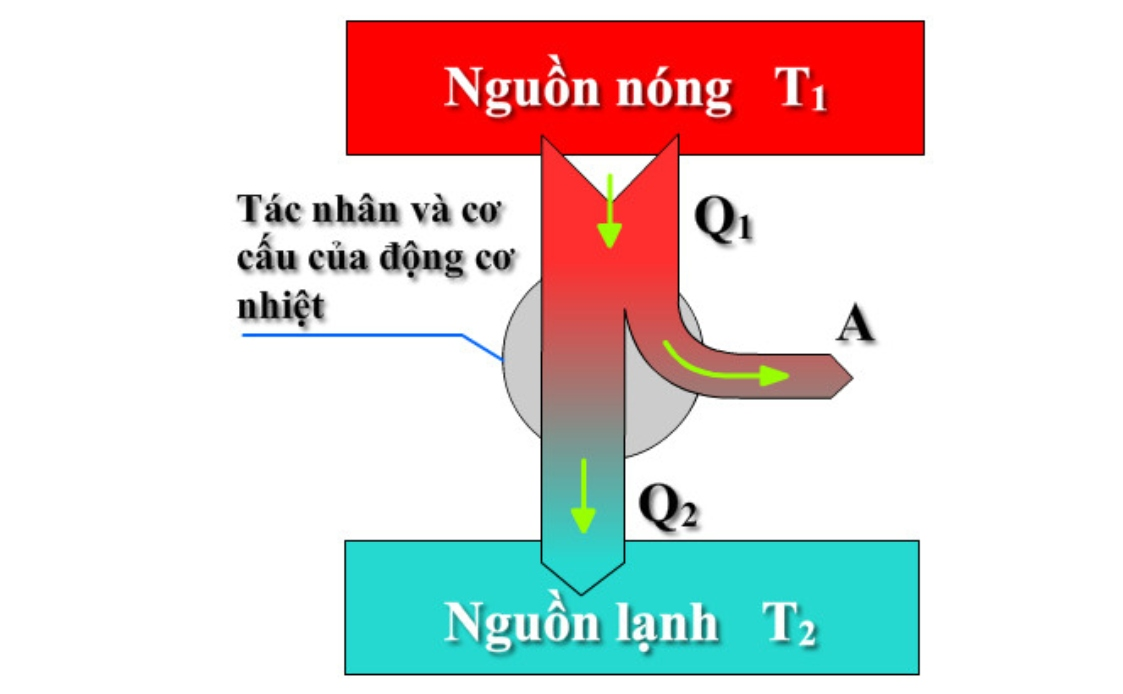
\includegraphics[scale=0.25]{figs/VN12-Y24-PH-SYL-007-1}
				\end{center}
				\item \textbf{Hiệu suất của động cơ nhiệt}\\
				$$H=\dfrac{A}{Q_1}=\dfrac{Q_1-Q_2}{Q_1}=1-\dfrac{Q_2}{Q_1}.$$
\begin{luuy}
	Động cơ nhiệt không thể chuyển đổi toàn bộ nhiệt lượng nhận được thành công $\left(H<1\right)$.\\
					Hiệu suất cực đại của động cơ nhiệt:
					$$H_\text{max}=\dfrac{T_1-T_2}{T_1}.$$
\end{luuy}
			\end{itemize}
\end{dang}
% =======================================
\begin{vd}
Một động cơ nhiệt làm việc sau một thời gian thì tác nhân đã nhận từ nguồn nóng nhiệt lượng $Q_1=\SI{1.5E6}{\joule}$, truyền cho nguồn lạnh nhiệt lượng $Q_2=\SI{1.2E6}{\joule}$. Hiệu suất thực của động cơ nhiệt này là bao nhiêu?
	\loigiai{
			Hiệu suất thực của động cơ nhiệt:
			$$H=1-\dfrac{Q_2}{Q_1}=1-\dfrac{\SI{1.2E6}{\joule}}{\SI{1.5E6}{\joule}}=\SI{20}{\percent}.$$
		}
\end{vd}
% ===============================================
\begin{vd}
Máy hơi nước công suất $\SI{10}{\kilo\watt}$ tiêu thụ $\SI{10}{\kilogram}$ than đá trong $\SI{1}{\text{giờ}}$. Biết hơi nước vào và ra cylanh có nhiệt độ $\SI{227}{\celsius}$ và $\SI{100}{\celsius}$. Năng suất toả nhiệt của than đá là $\SI{3.6E7}{\joule/\kilogram}$. Tính hiệu suất thực của máy và của một động cơ nhiệt lí tưởng làm việc với nhiệt độ nguồn nóng và nguồn lạnh nói trên.
\loigiai{
			Hiệu suất của một động cơ nhiệt lí tưởng hoạt động giữa hai nguồn nhiệt $\SI{227}{\celsius}$ và $\SI{100}{\celsius}$:
			$$T_1=t_1+273=\SI{500}{\kelvin};\quad T_2=t_2+273=\SI{373}{\kelvin}.$$
			$$H_\text{max}=\dfrac{T_1-T_2}{T_1}=\SI{25.4}{\percent}.$$
			Hiệu suất thực của động cơ:
			$$H=\dfrac{A}{Q}=\dfrac{\calP t}{mq}=\dfrac{\left(\SI{10E3}{\watt}\right)\cdot\left(\SI{3600}{\second}\right)}{\left(\SI{10}{\kilogram}\right)\cdot\left(\SI{3.6E7}{\joule/\kilogram}\right)}=\SI{10}{\percent}.$$}

\end{vd}
\subsection{BÀI TẬP TRẮC NGHIỆM}
\Opensolutionfile{ans}[ans/G12Y24B6TN]
% ===================================================================
\begin{ex}
	Một động cơ nhiệt lí tưởng thực hiện một công $\SI{5}{\kilo\joule}$ đồng thời truyền cho nguồn lạnh nhiệt lượng $\SI{15}{\kilo\joule}$. Hiệu suất của động cơ nhiệt này là
	\choice
	{$\SI{33.33}{\percent}$}
	{$\SI{75}{\percent}$}
	{\True $\SI{25}{\percent}$}
	{$\SI{66.67}{\percent}$}
	\loigiai{$$H=\dfrac{A}{Q_1}=\dfrac{A}{Q_2+A}=\SI{25}{\percent}.$$
	}
\end{ex}
% ===================================================================
\begin{ex}
	Một động cơ nhiệt làm việc giữa hai nguồn nhiệt. Nhiệt lượng tác nhân nhận của nguồn nóng trong một chu trình là $\SI{2400}{\joule}$. Hiệu suất của động cơ nhiệt là $\SI{25}{\percent}$. Nhiệt lượng tác nhân truyền cho nguồn lạnh trong một chu trình là
	
	\choice
	{$\SI{1200}{\joule}$}
	{$\SI{2400}{\joule}$}
	{$\SI{600}{\joule}$}
	{\True $\SI{1800}{\joule}$}
	\loigiai{$$H=1-\dfrac{Q_2}{Q_1}\Rightarrow Q_2=\SI{1800}{\joule}.$$
	}
\end{ex}
% ===================================================================
\begin{ex}
	Một động cơ nhiệt nhả cho nguồn lạnh $\SI{80}{\percent}$ nhiệt lượng mà nó thu được từ nguồn nóng. Hiệu suất của động cơ nhiệt này là
	
	\choice
	{\True $\SI{20}{\percent}$}
	{$\SI{37}{\percent}$}
	{$\SI{50}{\percent}$}
	{$\SI{80}{\percent}$}
	\loigiai{Hiệu suất của động cơ nhiệt:
		$$H=1-\dfrac{Q_2}{Q_1}=\SI{20}{\percent}.$$
	}
\end{ex}
% ===================================================================
\begin{ex}
	Người ta phải tốn $\SI{150}{\gram}$ dầu hoả để đun sôi được $\SI{4.5}{\text{lít}}$ nước ở nhiệt độ ban đầu $\SI{20}{\celsius}$. Cho biết khối lượng riêng của nước là $\SI{1}{\kilogram/\text{lít}}$, nhiệt dung riêng của nước là $\SI{4200}{\joule/\left(\kilogram\cdot\kelvin\right)}$, năng suất toả nhiệt của dầu hoả là $\SI{44E6}{\joule/\kilogram}$. Hiệu suất của bếp đun là
	
	\choice
	{\True $\SI{22.9}{\percent}$}
	{$\SI{2.29}{\percent}$}
	{$\SI{12.9}{\percent}$}
	{$\SI{26.9}{\percent}$}
	\loigiai{Hiệu suất của bếp đun:
		$$H=\dfrac{m_\text{n}c\Delta t}{m_\text{d}q}=\SI{22.9}{\percent}.$$
	}
\end{ex}
% ===================================================================
\begin{ex}
	Để đun sôi một lượng nước bằng bếp dầu có hiệu suất $\SI{30}{\percent}$, phải dùng hết 1 lít dầu. Để đun sôi cũng lượng nước trên với bếp dầu có hiệu suất $\SI{20}{\percent}$ thì phải dùng
	
	\choice
	{2 lít dầu}
	{0,5 lít dầu}
	{\True 1,5 lít dầu}
	{3 lít dầu}
	\loigiai{$$V_2=\dfrac{V_1H_1}{H_2}=\SI{1.5}{\liter}.$$
	}
\end{ex}
% ===================================================================
\begin{ex}
	Khi dùng lò có hiệu suất $H_1$ để làm chảy một lượng quặng, phải đốt hết $\xsi{m_1}{\left(\kilogram\right)}$ nhiên liệu có năng suất toả nhiệt $q_1$. Nếu dùng lò có hiệu suất $H_2$ để làm chảy lượng quặng trên thì phải đốt hết $m_2=\xsi{3m_1}{\left(\kilogram\right)}$ nhiên liệu có năng suất toả nhiệt $q_2=0,5q_1$. Hệ thức liên hệ giữa $H_1$ và $H_2$ là
	
	\choice
	{$H_1=H_2$}
	{$H_1=2H_2$}
	{$H_1=3H_2$}
	{\True $H_1=1,5H_2$}
	\loigiai{$$H=\dfrac{Q}{mq}$$
		$$\Rightarrow \dfrac{H_1}{H_2}=\dfrac{m_2q_2}{m_1q_1}=\dfrac{3}{2}.$$}
\end{ex}
% ===================================================================
\begin{ex}
	Một động cơ nhiệt có hiệu suất $\SI{25}{\percent}$ và công suất $\SI{30}{\kilo\watt}$. Nhiệt lượng mà động cơ toả ra cho nguồn lạnh trong 5 giờ làm việc liên tục là
	
	\choice
	{$\SI{176E7}{\joule}$}
	{$\SI{194E7}{\joule}$}
	{$\SI{213E7}{\joule}$}
	{\True $\SI{162E7}{\joule}$}
	\loigiai{$$H=\dfrac{A}{A+Q_2}=\dfrac{\calP t}{\calP t+Q_2}\Rightarrow Q_2=\SI{162E7}{\joule}.$$}
\end{ex}
% ===================================================================
\begin{ex}
	Một đầu máy diezen xe lửa có công suất $\SI{3E6}{\watt}$ và có hiệu suất $\SI{25}{\percent}$. Cho biết năng suất toả nhiệt của nhiên liệu là $\SI{4.2E7}{\joule/\kilogram}$. Nếu đầu máy chạy hết công suất thì khối lượng nhiên liệu tiêu thụ trong mỗi giờ \textbf{gần giá trị nào nhất} sau đây?
	
	\choice
	{$\SI{2489}{\kilogram}$}
	{$\SI{1429}{\kilogram}$}
	{\True $\SI{1028}{\kilogram}$}
	{$\SI{1056}{\kilogram}$}
	\loigiai{Khối lượng nhiên liệu tiêu thụ trong 1 giờ khi động cơ xe lửa hoạt động hết công suất:
		$$m=\dfrac{\calP t}{qH}\approx\SI{1028.57}{\kilogram}.$$
	}
\end{ex}
% ===================================================================
\begin{ex}
	Một máy bơm sau khi tiêu thụ hết $\SI{8}{\kilogram}$ dầu thì đưa được $\SI{700}{\meter^3}$ nước lên cao $\SI{8}{\meter}$. Biết năng suất toả nhiệt của dầu dùng cho  máy bơm này là $\SI{4.6E7}{\joule/\kilogram}$. Xem rằng nước được đưa lên cao một cách đều đặn, khối lượng riêng của nước $\SI{1000}{\kilogram/\meter^3}$, gia tốc trọng trường $g=\SI{10}{\meter/\second^2}$. Hiệu suất của máy bơm là
	
	\choice
	{\True $\SI{15.22}{\percent}$}
	{$\SI{24.46}{\percent}$}
	{$\SI{1.52}{\percent}$}
	{$\SI{2.45}{\percent}$}
	\loigiai{Hiệu suất máy bơm:
		$$H=\dfrac{\rho Vgh}{qm_\text{d}}\approx\SI{15.22}{\percent}.$$
	}
\end{ex}
% ===================================================================
\begin{ex}
	Một ô tô chạy $\SI{100}{\kilo\meter}$ với lực kéo không đổi $\SI{700}{\newton}$ thì tiêu thụ hết $\SI{6}{\text{lít}}$ xăng. Biết năng suất toả nhiệt của xăng là $\SI{4.6E7}{\joule/\kilogram}$, khối lượng riêng của xăng là $\SI{700}{\kilogram/\meter^3}$. Hiệu suất của động cơ ô tô là
	
	\choice
	{$\SI{25}{\percent}$}
	{\True $\SI{36}{\percent}$}
	{$\SI{0.36}{\percent}$}
	{$\SI{17.75}{\percent}$}
	\loigiai{Hiệu suất của động cơ ô tô:
		$$H=\dfrac{A}{Q}=\dfrac{Fs}{\rho_\text{xăng}Vq}=\SI{36.23}{\percent}.$$
	}
\end{ex}
% ===================================================================
\begin{ex}
	Một nhà máy điện tiêu thụ $\SI{0.35}{\kilogram}$ nhiên liệu cho mỗi $\SI{1}{\kilo\watt\hour}$ điện năng. Cho biết năng suất toả nhiệt của nhiên liệu trên là $\SI{42}{\mega\joule/\kilogram}$. Hiệu suất của động cơ nhiệt dùng trong nhà máy điện \textbf{gần nhất} với giá trị nào sau đây?
	
	\choice
	{$\SI{38}{\percent}$}
	{$\SI{15}{\percent}$}
	{$\SI{20}{\percent}$}
	{\True $\SI{24}{\percent}$}
	\loigiai{Hiệu suất của động cơ nhiệt dùng trong nhà máy:
		$$H=\dfrac{A}{Q_\text{tp}}=\dfrac{\left(\SI{E3}{\watt}\right)\cdot\left(\SI{3600}{\second}\right)}{\left(\SI{0.35}{\kilogram}\right)\cdot\left(\SI{42E6}{\joule/\kilogram}\right)}\approx\SI{24.5}{\percent}.$$}
\end{ex}
% ===================================================================
\begin{ex}
	Một chiếc xe máy hoạt động với công suất $\SI{3.2}{\kilo\watt}$ và chuyển động đều với tốc độ $\SI{45}{\kilo\meter/\hour}$. Hiệu suất của động cơ là $\SI{25}{\percent}$, năng suất toả nhiệt của xăng là $\SI{4.6E7}{\joule/\kilogram}$, khối lượng riêng của xăng là $\SI{700}{\kilogram/\meter^3}$. Với 2 lít xăng thì xe máy đi được bao nhiêu $\si{\kilo\meter}$?
	
	\choice
	{$\SI{100.6}{\kilo\meter}$}
	{\True $\SI{63}{\kilo\meter}$}
	{$\SI{45}{\kilo\meter}$}
	{$\SI{54}{\kilo\meter}$}
	\loigiai{Thời gian động cơ xe máy hoạt động được khi tiêu thụ $\SI{2}{\text{lít}}$ xăng:
		$$t=\dfrac{q\rho V}{\calP}\cdot H=\SI{5031.25}{\second}=\SI{1.39}{\hour}.$$
		Quãng đường xe máy đi được:
		$$s=vt\approx\SI{62.89}{\kilo\meter}.$$
	}
\end{ex}
% ===================================================================
\begin{ex}
	Một động cơ ô tô hoạt động với công suất $\SI{20}{\kilo\watt}$ và ô tô chuyển động đều với tốc độ $\SI{72}{\kilo\meter/\hour}$. Ô tô tiêu thụ $\SI{20}{\text{lít}}$ xăng thì chạy được quãng đường $\SI{200}{\kilo\meter}$. Biết khối lượng riêng của xăng là $\SI{700}{\kilogram/\meter^3}$, năng suất toả nhiệt của xăng là $\SI{4.6E7}{\joule/\kilogram}$. Hiệu suất của động cơ ô tô khi đó là
	
	\choice
	{\True $\SI{31}{\percent}$}
	{$\SI{61}{\percent}$}
	{$\SI{63}{\percent}$}
	{$\SI{36}{\percent}$}
	\loigiai{Hiệu suất của ô tô:
		$$H=\dfrac{\calP\cdot\dfrac{s}{v}}{\rho Vq}\approx\SI{31.05}{\percent}.$$
	}
\end{ex}
% ===================================================================
\begin{ex}
	Dùng một bếp dầu hoả để đun sôi 2 lít nước từ $\SI{15}{\celsius}$ thì mất $\SI{10}{\text{phút}}$. Biết rằng chỉ có $\SI{40}{\percent}$ nhiệt lượng do dầu toả ra làm nóng nước. Lấy nhiệt dung riêng của nước là $\SI{4190}{\joule/\left(\kilogram\cdot\kelvin\right)}$, năng suất toả nhiệt của dầu hoả là $\SI{46E6}{\joule/\kilogram}$, khối lượng riêng của nước là $\SI{1}{\gram/\centi\meter^3}$. Lượng dầu hoả cần dùng trong mỗi phút là
	\choice
	{$\SI{0.619}{\gram}$}
	{$\SI{0.619}{\kilogram}$}
	{\True $\SI{3.87}{\gram}$}
	{$\SI{3.87}{\kilogram}$}
	\loigiai{Khối lượng dầu cần dùng trong mỗi phút:
		$$m=\dfrac{Q}{qH}=\dfrac{mc\Delta t}{qH}=\SI{3.87E-3}{\kilogram}=\SI{3.87}{\gram}.$$
	}
\end{ex}
% ===================================================================
\begin{ex}
	Người ta cần nấu chảy 10 tấn đồng trong lò nung dùng dầu làm nhiên liệu đốt. Cho biết nhiệt độ ban đầu, nhiệt độ nóng chảy, nhiệt dung riêng và nhiệt nóng chảy riêng của đồng lần lượt là $\SI{13}{\celsius}$, $\SI{1083}{\celsius}$, $\SI{380}{\joule/\left(\kilogram\cdot\kelvin\right)}$, $\SI{1.8E5}{\joule/\kilogram}$. Nhiệt lượng toả ra khi đốt cháy $\SI{1}{\kilogram}$ dầu là $\SI{4.6E7}{\joule/\kilogram}$. Nếu hiệu suất nung của lò là $\SI{30}{\percent}$ thì khối lượng dầu cần dùng là
	\choice
	{\True $\SI{425.1}{\kilogram}$}
	{$\SI{127.5}{\kilogram}$}
	{$\SI{38.3}{\kilogram}$}
	{$\SI{432.2}{\kilogram}$}
	\loigiai{Nhiệt lượng đồng cần thu vào để nóng chảy hoàn toàn:
		$$Q=mc\Delta t+m\lambda=\SI{58.66E8}{\joule}.$$
		Khối lượng xăng cần dùng:
		$$m=\dfrac{Q}{qH}=\SI{425.1}{\kilogram}.$$
	}
\end{ex}
% ===================================================================
\begin{ex}
Một ấm nhôm có khối lượng $m_\text{b}=\SI{600}{\gram}$ chứa $V=\SI{1.5}{\text{lít}}$ nước ở $t_1=\SI{20}{\celsius}$, sau đó đun bằng bếp điện. Sau thời gian $t=\SI{35}{\text{phút}}$ thì đã có $\SI{20}{\percent}$ khối lượng nước đã hoá hơi ở nhiệt độ sôi $t_2=\SI{100}{\percent}$. Biết rằng, $\SI{75}{\percent}$ nhiệt lượng mà bếp cung cấp được dùng vào việc đun nước. Cho biết nhiệt dung riêng của nước là $c_\text{n}=\SI{4190}{\joule/\left(\kilogram\cdot\kelvin\right)}$, của nhôm là $c_\text{b}=\SI{880}{\joule/\left(\kilogram\cdot\kelvin\right)}$, nhiệt hoá hơi riêng của nước ở $\SI{100}{\celsius}$ là $L=\SI{2.26E6}{\joule/\kilogram}$, khối lượng riêng của nước là $D=\SI{1}{\kilogram/\text{lít}}$. Công suất cung cấp nhiệt của bếp điện \textbf{gần giá trị nào nhất} sau đây?	
	\choice
	{\True $\SI{776}{\watt}$}
	{$\SI{796}{\watt}$}
	{$\SI{786}{\watt}$}
	{$\SI{876}{\watt}$}
	\loigiai{Khối lượng nước $$m_\text{n}=VD=\SI{1.5}{\kilogram}.$$
		Tổng nhiệt lượng nước và ấm thu vào:
		$$Q=\left(m_\text{n}c_\text{n}+m_\text{b}c_\text{b}\right)\cdot\left(t_2-t_1\right)+\SI{20}{\percent}m_\text{n}L=\SI{1223040}{\joule}.$$
		Điện năng tiêu thụ của ấm:
		$$A=\dfrac{Q}{H}=\SI{1630720}{\joule}.$$
		Công suất của ấm điện:
		$$\calP=\dfrac{A}{t}\approx\SI{776.5}{\watt}.$$	}
\end{ex}
\Closesolutionfile{ans}
	\subsection{TRẮC NGHIỆM ĐÚNG/SAI}
	\setcounter{ex}{0}
	% ================================
	\begin{ex}
		\immini{
	Cầu chì là linh kiện được sử dụng để bảo vệ thiết bị và lưới điện tránh sự cố ngắn mạch, hạn chế tình trạng cháy, nổ.
	\begin{enumerate}[label=\alph*)]
		\item Cầu chì có thể bảo vệ mạch điện dựa trên sự phụ thuộc của điện trở kim loại theo nhiệt độ.
		\item Dây chảy trong cầu chì thường được làm từ kim loại có nhiệt độ nóng chảy cao.
		\item Khi cường độ dòng điện qua mạch tăng vượt hạn, dây chì sẽ nóng chảy trước.
		\item Khi dây chảy trong cầu chì bị đứt, ta có thể nối cầu chì bằng dây sắt.
	\end{enumerate}	
	}{
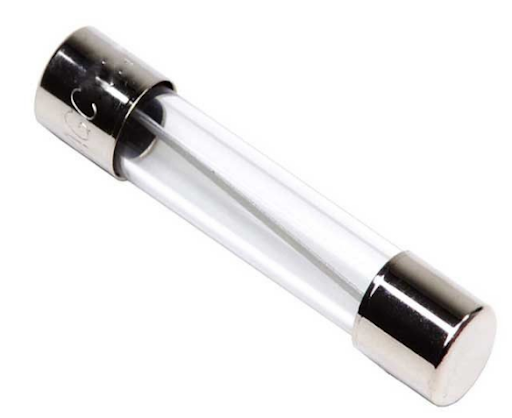
\includegraphics[scale=0.2]{figs/VN12-Y24-PH-SYL-007P-1}
}
\loigiai{
\begin{enumerate}[label=\alph*)]
	\item Sai. Khi dòng điện qua mạch vượt hạn, dây chảy trong cầu chì nóng chảy trước và là hở mạch.
	\item Sai. Dây chảy được làm từ kim loại có nhiệt độ nóng chảy thấp.
	\item Đúng.
	\item Sai. Sắt là kim loại có nhiệt độ nóng chảy cao, khi cường độ dòng điện tăng quá lớn nhưng dây sắt nóng chảy chậm nên không bảo vệ được mạch điện.
\end{enumerate}
}
		\end{ex}
	\subsection{BÀI TẬP TỰ LUẬN}
	\setcounter{ex}{0}
% ===================================================================
\begin{ex}
	Một bếp dầu đun sôi 1 lít nước đựng trong ấm bằng nhôm khối lượng $m_2=\SI{300}{\gram}$ thì sau thời gian $t_1=\SI{10}{\minute}$ nước sôi. Nếu dùng bếp trên để đun 2 lít nước trong cùng điều kiện thì sau bao lâu nước sôi? Cho nhiệt dung riêng của nước và nhôm lần lượt là $c_1=\SI{4200}{\joule/\left(\kilogram\cdot\kelvin\right)}$, $c_2=\SI{880}{\joule/\left(\kilogram\cdot\kelvin\right)}$. Biết nhiệt do bếp dầu cung cấp một cách đều đặn.
	\loigiai{Vì bếp dầu cung cấp nhiệt lượng một cách đều đặn nên
		$$\dfrac{t_2}{t_1}=\dfrac{\left(m_2c_2+m'_1c_1\right)\Delta t}{\left(m_2c_2+m_1c_1\right)\Delta t}=\dfrac{m_2c_2+m'_1c_1}{m_2c_2+m_1c_1}\Rightarrow t_2\approx\SI{19.4}{\minute}.$$}
\end{ex}
% ===================================================================
\begin{ex}
	Khi thả một quả cầu nhôm khối lượng $\SI{500}{\gram}$ vào $\SI{2}{\kilogram}$ nước ở $\SI{25}{\celsius}$ thì nhiệt độ của chúng sau khi cân bằng nhiệt là $\SI{30}{\celsius}$. Hỏi nhiệt độ ban đầu của quả cầu nhôm là bao nhiêu? Biết nhiệt lượng hao phí trong trường hợp này bằng $\SI{20}{\percent}$ nhiệt lượng do nước thu vào. Biết nhiệt dung riêng của nhôm là $\SI{880}{\joule/\left(\kilogram\cdot\kelvin\right)}$, nhiệt dung riêng của nước là $\SI{4200}{\joule/\left(\kilogram\cdot\kelvin\right)}$. Bỏ qua sự hoá hơi của nước ngay khi tiếp xúc với quả cầu.
	
	\loigiai{Khi hệ cân bằng nhiệt, tổng nhiệt lượng trao đổi trong hệ bằng 0:
		\begin{eqnarray*}
			&&Q_1+Q_2+Q_\text{hp}=0\\
			&\Leftrightarrow& m_1C_1\left(t_\text{cb}-t_1\right)+1,2m_2C_2\left(t_\text{cb}-t_2\right)=0\\
			&\Rightarrow& t_1\approx\SI{144.55}{\celsius}.
	\end{eqnarray*}}
\end{ex}
% ===================================================================
\begin{ex}
	Động cơ nhiệt lí tưởng làm việc giữa hai nguồn nhiệt $\SI{27}{\celsius}$ và $\SI{127}{\celsius}$. Nhiệt lượng tác nhân nhận từ nguồn nóng trong một chu trình là $\SI{2400}{\joule}$. Tính:
	\begin{enumerate}[label=\alph*)]
		\item hiệu suất của động cơ.
		\item công thực hiện trong một chu trình.
		\item nhiệt lượng truyền cho nguồn lạnh trong một chu trình.
	\end{enumerate}
	
	\loigiai{\begin{enumerate}[label=\alph*)]
			\item $H=\dfrac{T_1-T_2}{T_1}=\SI{25}{\percent}.$
			\item $A=H\cdot Q_1=\SI{600}{\joule}$.
			\item $Q_2=Q_1-A=\SI{1800}{\joule}$.
		\end{enumerate}
	}
\end{ex}
% ===================================================================
\begin{ex}
	Máy hơi nước công suất $\SI{1}{\kilo\watt}$ tiêu thụ $\SI{10}{\kilogram}$ than đá trong 1 giờ. Biết hơi nước vào và ra cylanh có nhiệt độ $\SI{227}{\celsius}$ và $\SI{100}{\celsius}$. Năng suất toả nhiệt của than đá là $\SI{3.6E7}{\joule/\kilogram}$. Tính hiệu suất thực của máy và của một động cơ nhiệt lý tưởng làm việc giữa hai nhiệt độ nói trên.
	
	\loigiai{Hiệu suất của máy:
		$$H=\dfrac{A}{Q}=\dfrac{\calP t}{mq}=\SI{10}{\percent}.$$
		Hiệu suất của động cơ nhiệt lí tưởng:
		$$H_\text{max}=\dfrac{T_1-T_2}{T_1}=\SI{25.4}{\percent}.$$
	}
\end{ex}
% ===================================================================
\begin{ex}
	Một động cơ hơi nước lí tưởng là động cơ nhiệt có hiệu suất cực đại, hoạt động với nguồn nóng là lò hơi có nhiệt độ $\SI{500}{\kelvin}$. Nước được đưa vào lò hơi và được đun nóng để chuyển thể thành hơi nước. Hơi nước này làm piston chuyển động. Nhiệt độ của nguồn lạnh là nhiệt độ bên ngoài của không khí, bằng $\SI{300}{\kelvin}$.
	\begin{enumerate}[label=\alph*)]
		\item Tính công của động cơ hơi nước thực hiện khi lò hơi cung cấp cho tác nhân một nhiệt lượng bằng $\SI{6.5E3}{\joule}$.
		\item Giả sử muốn tăng hiệu suất này lên $\SI{45}{\percent}$ phải tăng nhiệt độ lò hơi lên một lượng bằng bao nhiêu?
	\end{enumerate}
	
	\loigiai{\begin{enumerate}[label=\alph*)]
			\item $H=\dfrac{A}{Q_1}=\dfrac{T_1-T_2}{T_1}\Rightarrow A=\SI{2600}{\joule}$.
			\item $H_\text{max}=\dfrac{T_1-T_2}{T_1}\Rightarrow T_1\approx\SI{545.46}{\kelvin}.$
		\end{enumerate}
	}
\end{ex}
% ===================================================================
\begin{ex}
	Búa máy 10 tấn rơi từ độ cao $\SI{2.3}{\meter}$ xuống một cọc sắt khối lượng $\SI{200}
	{\kilogram}$. Biết $\SI{40}{\percent}$ động năng của búa biến thành nhiệt làm nóng cọc sắt. Hỏi búa rơi bao nhiêu lần thì cọc tăng nhiệt độ thêm $\SI{20}{\celsius}$. Cho rằng cọc không toả nhiệt ra môi trường và nhiệt dung riêng của sắt là $\SI{0.46}{\kilo\joule/\left(\kilogram\cdot\kelvin\right)}$.
	\loigiai{\begin{itemize}
			\item Động năng của búa ngay trước khi va chạm với cọc: $W_\text{đ}=Mgh$.
			\item Nhiệt lượng cọc thu được sau mỗi lần búa rơi: $Q_0=0,4W_\text{đ}=0,4Mgh$.
			\item Nhiệt lượng cọc thu được sau $n$ lần búa rơi: $Q=nQ_0=mc\Delta t$.
		\end{itemize}
		Suy ra:
		$$n=\dfrac{mc\Delta t}{0,4Mgh}=20.$$
	}
\end{ex}

	
%\newpage\section*{ÔN TẬP CHƯƠNG I}
\subsection{Câu trắc nghiệm nhiều phương án lựa chọn}
\textit{Thí sinh trả lời từ câu 1 đến câu 18. Mỗi câu hỏi thí sinh chọn một phương án}
\Opensolutionfile{ans}[ans/G12Y24B7TN]
% ===================================================================
\begin{ex}
	Quy ước dấu nào sau đây phù hợp với định luật I của nhiệt động lực học?
	\choice
	{Vật nhận công $A<0$; vật nhận nhiệt $Q<0$}
	{Vật thực hiện công $A>0$; vật truyền nhiệt lượng $Q<0$}
	{\True Vật nhận công $A>0$; vật nhận nhiệt lượng $Q>0$}
	{Vật thực hiện công $A>0$; vật truyền nhiệt lượng $Q>0$}
	\loigiai{}
\end{ex}
% ===================================================================
\begin{ex}
	Ở nhiệt độ phòng, chất nào sau đây không tồn tại ở thể lỏng?
	\choice
	{Rượu}
	{\True Nhôm}
	{Thuỷ ngân}
	{Nước}
	\loigiai{}
\end{ex}
% ===================================================================
\begin{ex}
	Vật nào sau đây có cấu trúc tinh thể?
	\choice
	{\True Chiếc cốc thuỷ tinh}
	{Hạt muối ăn}
	{Viên kim cương}
	{Miếng thạch anh}
	\loigiai{}
\end{ex}
% ===================================================================
\begin{ex}
Điều nào sau đây là \textbf{sai} khi nói về sự đông đặc?	
	\choice
	{Sự đông đặc là quá trình chuyển từ thể lỏng sang thể rắn}
	{\True Với một chất rắn, nhiệt độ đông đặc luôn nhỏ hơn nhiệt độ nóng chảy}
	{Trong suốt quá trình đông đặc, nhiệt độ của vật không thay đổi}
	{Nhiệt độ đông đặc của các chất thay đổi theo áp suất bên ngoài}
	\loigiai{}
\end{ex}
% ===================================================================
\begin{ex}
	Biểu thức nào sau đây là biểu thức chuyển đổi đúng đơn vị nhiệt độ từ $\si{\celsius}$ sang thang $\si{\kelvin}$?
	\choice
	{\True $\xsi{T}{\left(\si{\kelvin}\right)}=\xsi{t}{\left(\si{\celsius}\right)}+273$}
	{$\xsi{T}{\left(\si{\kelvin}\right)}=\xsi{t}{\left(\si{\celsius}\right)}-273$}
	{$\xsi{T}{\left(\si{\kelvin}\right)}=\dfrac{9}{5}\xsi{t}{\left(\si{\celsius}\right)}+273$}
	{$\xsi{T}{\left(\si{\kelvin}\right)}=\dfrac{9}{5}\xsi{t}{\left(\si{\celsius}\right)}-273$}
	\loigiai{}
\end{ex}
% ===================================================================
\begin{ex}
	Trong thang nhiệt độ Celsius, nhiệt độ không tuyệt đối là
	\choice
	{$\SI{100}{\celsius}$}
	{\True $\SI{-273}{\celsius}$}
	{$\SI{0}{\celsius}$}
	{$\SI{-32}{\celsius}$}
	\loigiai{}
\end{ex}
% ===================================================================
\begin{ex}
	Đơn vị nhiệt nóng chảy riêng của vật rắn là
	\choice
	{$\si{\joule}$}
	{$\si{\joule/\kelvin}$}
	{\True $\si{\joule/\kilogram}$}
	{$\si{\joule/\left(\kilogram\cdot\kelvin\right)}$}
	\loigiai{}
\end{ex}

% ===================================================================
\begin{ex}
	Kết luận nào sau đây \textbf{không đúng} với thang nhiệt độ Celsius?
	\choice
	{Đơn vị đo nhiệt độ là $\si{\celsius}$}
	{Chọn mốc nhiệt độ nước đá đang tan ở áp suất $\SI{1}{atm}$ là $\SI{0}{\celsius}$}
	{Chọn mốc nhiệt độ nước sôi ở áp suất $\SI{1}{atm}$ là $\SI{100}{\celsius}$}
	{\True $\SI{1}{\celsius}$ tương ứng với $\SI{273}{\kelvin}$}
	\loigiai{}
\end{ex}
% ===================================================================
\begin{ex}
	Nhiệt hoá hơi riêng của nước là $\SI{2.3E6}{\joule/\kilogram}$. Phát biểu nào dưới đây là \textbf{đúng}?
	\choice
	{\True Mỗi kilogram nước cần thu một lượng nhiệt $\SI{2.3E6}{\joule}$ để bay hơi hoàn toàn ở nhiệt độ sôi và áp suất chuẩn}
	{Mỗi kilogram nước cần thu một lượng nhiệt $\SI{2.3E6}{\joule}$ để bay hơi hoàn toàn}
	{Mỗi kilogram nước cần toả ra một lượng nhiệt $\SI{2.3E6}{\joule}$ để bay hơi hoàn toàn ở nhiệt độ sôi}
	{Một lượng nước bất kì cần thu một lượng nhiệt là $\SI{2.3E6}{\joule}$ để bay hơi hoàn toàn}
	\loigiai{}
\end{ex}
% ===================================================================
\begin{ex}
	Hãy tìm ý \textbf{không đúng} với mô hình động học phân tử.
	\choice
	{\True Tốc độ chuyển động của các phân tử cấu tạo nên vật càng lớn thì thể tích của vật càng lớn}
	{Các chất được cấu tạo từ các hạt riêng biệt gọi là phân tử}
	{Các phân tử chuyển động không ngừng}
	{Giữa các phân tử có lực tương tác gọi là lực liên kết phân tử}
	\loigiai{}
\end{ex}
% ===================================================================
\begin{ex}
	Điểm đóng băng và điểm sôi của nước theo thang nhiệt độ Kelvin là
	\choice
	{\True $\SI{273}{\kelvin}$ và $\SI{373}{\kelvin}$}
	{$\SI{0}{\kelvin}$ và $\SI{100}{\kelvin}$}
	{$\SI{73}{\kelvin}$ và $\SI{37}{\kelvin}$}
	{$\SI{32}{\kelvin}$ và $\SI{212}{\kelvin}$}
	\loigiai{}
\end{ex}
% ===================================================================
\begin{ex}
	Người ta cung cấp cho khí trong một cylanh nằm ngang nhiệt lượng $\SI{2}{\joule}$. Đồng thời nén piston một đoạn $\SI{5}{\centi\meter}$ với một lực có độ lớn là $\SI{20}{\newton}$. Độ biến thiên nội năng của khí là
	\choice
	{\True $\SI{3}{\joule}$}
	{$\SI{1}{\joule}$}
	{$\SI{-1}{\joule}$}
	{$\SI{-3}{\joule}$}
	\loigiai{$$\Delta U=Q+A=Q+F\cdot s=\SI{3}{\joule}.$$
	}
\end{ex}
% ===================================================================
\begin{ex}
	Nhiệt lượng cần cung cấp cho $\SI{0.5}{\kilogram}$ nước ở $\SI{0}{\celsius}$ đến khi nó sôi là bao nhiêu? Biết nhiệt dung riêng của nước là $\SI{4180}{\joule/\left(\kilogram\cdot\kelvin\right)}$.
	\choice
	{$\SI{5E5}{\joule}$}
	{$\SI{3E5}{\joule}$}
	{$\SI{4.18E5}{\joule}$}
	{\True $\SI{2.09E5}{\joule}$}
	\loigiai{$$Q=mc\Delta t=\SI{2.09E5}{\joule}.$$
	}
\end{ex}
% ===================================================================
\begin{ex}
	Biết nhiệt dung riêng của nước là $\SI{4200}{\joule/\left(\kilogram\cdot\kelvin\right)}$, nhiệt nóng chảy riêng của nước đá là $\SI{3.4E5}{\joule/\kilogram}$. Nhiệt lượng cần cung cấp cho $\SI{2}{\kilogram}$ nước đá ở nhiệt độ $\SI{0}{\celsius}$ là bao nhiêu để tăng nhiệt độ lên $\SI{60}{\celsius}$ là
	\choice
	{$\SI{0.72E6}{\joule}$}
	{\True $\SI{1.184E6}{\joule}$}
	{$\SI{2.254E6}{\joule}$}
	{$\SI{1.548E6}{\joule}$}
	\loigiai{Nhiệt lượng cần cung cấp cho $\SI{2}{\kilogram}$ nước đá ở nhiệt độ $\SI{0}{\celsius}$ là bao nhiêu để chuyển lên nhiệt độ $\SI{60}{\celsius}$ là
		$$Q=m\lambda+mc\Delta t=\SI{1.184E6}{\joule}.$$
	}
\end{ex}
% ===================================================================
\begin{ex}
Một lượng nước và một lượng rượu có thể tích bằng nhau, được cung cấp các nhiệt lượng tương ứng là $Q_1$ và $Q_2$. Biết khối lượng riêng của nước là $\SI{1000}{\kilogram/\meter^3}$ và của rượt là $\SI{800}{\kilogram/\meter^3}$, nhiệt dung riêng của nước và rượu lần lượt là $\SI{4200}{\joule/\left(\kilogram\cdot\kelvin\right)}$ và $\SI{2500}{\joule/\left(\kilogram\cdot\kelvin\right)}$. Để độ tăng nhiệt độ của nước và rượu bằng nhau thì
	\choice
	{$Q_1=Q_2$}
	{$Q_1=1,68Q_2$}
	{$Q_1=1,25Q_2$}
	{\True $Q_1=2,10Q_2$}
	\loigiai{$$\dfrac{Q_1}{Q_2}=\dfrac{m_1c_1}{m_2c_2}=\dfrac{\rho_1c_1}{\rho_2c_2}=2,1.$$
	}
\end{ex}
% ===================================================================
\begin{ex}
	Một ấm đun nước bằng nhôm có khối lượng $\SI{400}{\gram}$, chứa 3 lít nước được đun trên bếp. Khi nhận nhiệt lượng $\SI{740}{\kilo\joule}$ thì ấm đạt đến nhiệt độ $\SI{80}{\celsius}$. Biết nhiệt dung riêng của nhôm là $\SI{880}{\joule/\left(\kilogram\cdot\kelvin\right)}$, nhiệt dung riêng của nước là $\SI{4190}{\joule/\left(\kilogram\cdot\kelvin\right)}$. Coi nhiệt lượng mà ấm toả ra bên ngoài là không đáng kể. Nhiệt độ ban đầu của ấm và nước là
	\choice
	{$\SI{45.2}{\celsius}$}
	{\True $\SI{22.7}{\celsius}$}
	{$\SI{37.2}{\celsius}$}
	{$\SI{16.7}{\celsius}$}
	\loigiai{$$\Delta t=\dfrac{Q}{m_1c_1+m_2c_2}=\SI{57.27}{\celsius}\Rightarrow t_0=\SI{22.7}{\celsius}.$$
	}
\end{ex}
% ===================================================================
\begin{ex}
	Người ta thực hiện công $\SI{100}{\joule}$ để nén khí trong một cylanh. Biết khí truyền ra môi trường xung quanh nhiệt lượng $\SI{30}{\joule}$ thì độ biến thiên nội năng của khí là
	\choice
	{$\SI{30}{\joule}$}
	{$\SI{130}{\joule}$}
	{\True $\SI{70}{\joule}$}
	{$\SI{100}{\joule}$}
	\loigiai{Độ biến thiên nội năng của khí:
		$$\Delta U=A+Q=\SI{100}{\joule}-\SI{30}{\joule}=\SI{70}{\joule}.$$
	}
\end{ex}
% ===================================================================
\begin{ex}
	Một lượng khí khi bị nung nóng đã tăng thể tích thêm $\SI{0.02}{\meter^3}$ và nội năng biến thiên $\SI{1280}{\joule}$. Biết trong quá trình thay đổi thể tích thì áp suất khí luôn bằng $\SI{2E5}{\pascal}$. Nhiệt lượng đã truyền cho khí là
	\choice
	{$\SI{2720}{\joule}$}
	{$\SI{1280}{\joule}$}
	{\True $\SI{5280}{\joule}$}
	{$\SI{4000}{\joule}$}
	\loigiai{Công khối khí thực hiện trong quá trình dãn nở:
		$$A'=F\cdot \Delta x=pS\Delta x=p\Delta V=\SI{4000}{\joule}.$$
		Nhiệt lượng mà khí đã nhận:
		$$Q=\Delta U-A=\Delta U+A'=\SI{5280}{\joule}.$$
	}
\end{ex}

\Closesolutionfile{ans}
\subsection{CÂU TRẮC NGHIỆM ĐÚNG/SAI}
\setcounter{ex}{0}
\textit{Thí sinh trả lời từ câu 1 đến câu 4. Trong mỗi ý \textbf{a)}, \textbf{b)}, \textbf{c)}, \textbf{d)} ở mỗi câu, thí sinh chọn đúng hoặc sai.}

% ===================================================================
\begin{ex}
Nhận định về các phát biểu sau khi nói về đặc điểm của các chất rắn, lỏng, khí.	
\begin{enumerate}[label=\alph*)]
	\item Các phân tử ở thể lỏng có khoảng cách giữa các phân tử nhỏ hơn khi ở thể rắn.
	\item Các phân tử trong thể khí tự do di chuyển và không bị ràng buộc bởi lực tương tác giữa chúng.
	\item Vật ở thể lỏng không có thể tích riêng, nhưng có hình dạng riêng.
	\item Vật ở thể rắn có thể tích và hình dạng riêng, rất khó nén.
\end{enumerate}
	\loigiai{\begin{enumerate}
			\item Sai. Các phân tử thể lỏng có khoảng cách giữa các phân tử lớn hơn khi ở thể rắn.
			\item Sai. Có lực tương tác phân tử nhưng rất yếu.
			\item Sai. Vật ở thể lỏng có thể tích riêng, nhưng không có hình dạng riêng.
			\item Đúng.
	\end{enumerate}}
\end{ex}
% ===================================================================
\begin{ex}
Nhận định các phát biểu sau về nội năng của một hệ.
\begin{enumerate}[label=\alph*)]
	\item Nội năng của một vật phụ thuộc vào nhiệt độ và thể tích của vật.
	\item Nội năng của một vật thay đổi trong quá trình truyền nhiệt và trong quá trình thực hiện công.
	\item Nội năng của vật A lớn hơn nội năng của vật B thì nhiệt độ của vật A lớn hơn nhiệt độ của vật B.
	\item Nội năng có thể chuyển hoá hoàn toàn thành cơ năng.
\end{enumerate}	
	\loigiai{
		\begin{enumerate}[label=\alph*)]
			\item Đúng.
			\item Đúng.
			\item Sai. Nội năng của hệ không chỉ phụ thuộc vào nhiệt độ của hệ mà còn phụ thuộc vào thể tích của hệ.
			\item Sai. Nội năng của hệ không thể chuyển hoá hoàn toàn thành cơ năng.
	\end{enumerate}}
\end{ex}
% ===================================================================
\begin{ex}
	Một động cơ nhiệt lý tưởng hoạt động giữa hai nguồn nhiệt $\SI{100}{\celsius}$ và $\SI{24.5}{\celsius}$ thì thực hiện công $\SI{2}{\kilo\joule}$.
	\begin{enumerate}[label=\alph*)]
		\item Hiệu suất của động cơ là $\SI{0.2}{}$.
		\item Nhiệt lượng động cơ nhận từ nguồn nóng là $\SI{0.1}{\kilo\joule}$.
		\item Nhiệt lượng động cơ cung cấp cho nguồn lạnh là $\SI{1.9}{\kilo\joule}$.
		\item Để động cơ đạt hiệu suất $\SI{30}{\percent}$ thì phải tăng nhiệt độ nguồn nóng lên $\SI{152}{\celsius}$.
	\end{enumerate}
	
	\loigiai{\begin{enumerate}[label=\alph*)]
			\item Đúng.
			\item Đúng.
			\item Sai. Nhiệt lượng động cơ cung cấp cho nguồn lạnh là $\SI{7.88}{\kilo\joule}$.
			\item Đúng. 
	\end{enumerate}}
\end{ex}
% ===================================================================
\begin{ex}
	Dùng bếp điện để đun một ấm nhôm khối lượng $\SI{600}{\gram}$ đựng $\SI{1.5}{\text{lít}}$ nước ở nhiệt độ $\SI{20}{\celsius}$. Sau $\SI{35}{\minute}$ đã có $\SI{20}{\percent}$ lượng nước trong ấm hoá hơi ở nhiệt độ sôi $\SI{100}{\celsius}$. Biết có $\SI{60}{\percent}$ nhiệt lượng mà bếp toả ra được dùng vào việc đun ấm nước. Cho nhiệt dung riêng của nhôm là $\SI{880}{\joule/\left(\kilogram\cdot\kelvin\right)}$, của nước là $\SI{4200}{\joule/\left(\kilogram\cdot\kelvin\right)}$, nhiệt hoá hơi riêng của nước ở nhiệt độ sôi $\SI{100}{\celsius}$ là $\SI{2.26E6}{\joule/\kilogram}$ và khối lượng riêng của nước là $\SI{1}{\kilogram/\text{lít}}$.
	\begin{enumerate}[label=\alph*)]
		\item Nhiệt lượng cần thiết để đun ấm nước từ $\SI{20}{\celsius}$ đến $\SI{100}{\celsius}$ là $\SI{504000}{\joule}$.
		\item Khối lượng nước đã hoá hơi là $\SI{0.03}{\kilogram}$.
		\item Nhiệt lượng mà bếp điện cung cấp để đun nước đến khi sôi là $\SI{910.4}{\kilo\joule}$.
		\item Nhiệt lượng trung bình mà bếp điện cung cấp cho ấm nước trong mỗi giây là $\SI{582.97}{\joule}$.
	\end{enumerate}
	\loigiai{\begin{enumerate}[label=\alph*)]
			\item Sai. Nhiệt lượng cần thiết để đun sôi ấm nước là $\SI{546240}{\joule}$.
			\item Đúng.
			\item Đúng.
			\item Sai. Nhiệt lượng trung bình mà bếp điện cung cấp cho ấm nước trong mỗi giây là $\SI{971.6}{\joule}$.
		\end{enumerate}
	}
\end{ex}
\subsection{CÂU TRẮC NGHIỆM TRẢ LỜI NGẮN}
\setcounter{ex}{0}
\textit{Thí sinh trả lời từ câu 1 đến câu 6.}
% ===================================================================
\begin{ex}
Giả sử rằng các tuabin ở nhà máy nhiệt điện đã được nâng cấp, dẫn đến sự cải thiện về hiệu suất $\SI{3.32}{\percent}$. Biết rằng trước khi nâng cấp thì hiệu suất của nhà máy điện là $\SI{36}{\percent}$, nhiệt lượng truyền vào động cơ trong một ngày vẫn không đổi và bằng $\SI{2.5E14}{\joule}$. Có thêm bao nhiêu lượng điện năng được sản xuất trong 1 ngày nhờ vào sự nâng cấp trên \textit{(tính theo đơn vị  $\SI{E12}{\joule}$)}?
	\loigiai{$$\Delta A=Q_1\Delta H=\left(\SI{2.5E14}{\joule}\right)\cdot\left(\SI{3.32}{\percent}\right)=\SI{8.3E12}{\joule}.$$
	}
\end{ex}
% ===================================================================
\begin{ex}
	Người ta thả một miếng đồng khối lượng $\SI{0.5}{\kilogram}$ vào $\SI{500}{\gram}$ nước. Miếng đồng nguội đi từ $\SI{80}{\celsius}$ xuống $\SI{20}{\celsius}$. Hỏi nước nóng lên thêm bao nhiêu $\si{\celsius}$ \textit{(làm tròn đến 2 số thập phân)}? Biết nhiệt dung riêng của đồng là $\SI{380}{\joule/\left(\kilogram\cdot\kelvin\right)}$, nhiệt dung riêng của nước là $\SI{4200}{\joule/\left(\kilogram\cdot\kelvin\right)}$.
	\loigiai{$$\Delta t=\dfrac{m_\text{đ}c_\text{đ}\left(80-20\right)}{m_\text{n}c_\text{n}}\approx\SI{5.43}{\celsius}.$$}
\end{ex}
% ===================================================================
\begin{ex}
Một ấm điện có công suất $\SI{1000}{\watt}$. Tính thời gian cần thiết để đun sôi $\SI{0.5}{\text{lít}}$ nước có nhiệt độ ban đầu là $\SI{20}{\celsius}$ ở áp suất tiêu chuẩn theo đơn vị phút. Bỏ qua sự trao đổi nhiệt với vỏ ấm và môi trường. Cho hiệu suất ấm đun là $\SI{40}{\percent}$. Biết nhiệt dung riêng của nước là $\SI{4200}{\joule/\left(\kilogram\cdot\kelvin\right)}$ và khối lượng riêng của nước là $\SI{1}{\kilogram/\liter}$.
	\loigiai{$$t=\dfrac{mc\Delta t}{H\calP}\approx\SI{7}{\minute}.$$
	}
\end{ex}
% ===================================================================
\begin{ex}
	Tính nhiệt lượng cần cung cấp \textit{(theo đơn vị $\si{\kilo\joule})$} cho $\SI{10}{\kilogram}$ nước ở $\SI{30}{\celsius}$ chuyển thành hơi ở $\SI{100}{\celsius}$. Cho biết nhiệt dung riêng của nước $\SI{4180}{\joule/\left(\kilogram\cdot\kelvin\right)}$ và nhiệt hoá hơi riêng của nước là $\SI{2.3E6}{\joule/\kilogram}$.
	\loigiai{$$Q=mc\Delta t+mL=\SI{25926}{\kilo\joule}.$$
	}
\end{ex}
% ===================================================================
\begin{ex}
	\immini{
	10 viên nước đá được dùng để làm lạnh cốc nước soda có khối lượng $\SI{0.25}{\kilogram}$, mỗi viên đá có khối lượng $\SI{6}{\gram}$. Ban đầu, nước soda trong cốc có nhiệt độ $\SI{20}{\celsius}$. Xác định nhiệt độ cốc nước khi đá tan hết theo đơn vị $\si{\celsius}$ và làm tròn đến 2 chữ số thập phân. Biết rằng nhiệt dung riêng của nước là $\SI{4186}{\joule/\left(\kilogram\cdot\kelvin\right)}$, nhiệt nóng chảy riêng của nước đá là $\SI{3.34E5}{\joule/\kilogram}$. Bỏ qua sự trao đổi nhiệt với cốc và môi trường bên ngoài.
}
{
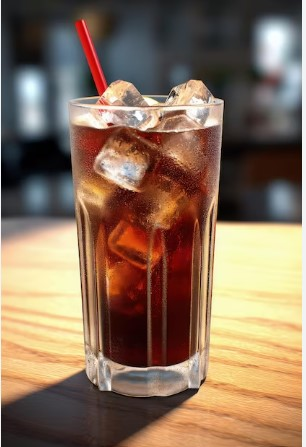
\includegraphics[scale=0.25]{figs/VN12-Y24-PH-SYL-008-1}
}
	\loigiai{Khi có cân bằng nhiệt, tổng nhiệt lượng trao đổi trong hệ bằng 0:
		$$10m_\text{đ}\lambda+m_\text{n}c_\text{n}\left(t_\text{cb}-t_0\right)=0$$
		$$\Rightarrow t_\text{cb}\approx\SI{0.69}{\celsius}.$$}
\end{ex}
% ===================================================================
\begin{ex}
	Năm 1986, một tảng băng khổng lồ đã tách ra khỏi thềm băng Ross ở Nam Cực. Tảng băng có dạng gần như hình hộp chữ nhật với chiều dài $\SI{160}{\kilo\meter}$, chiều rộng $\SI{40}{\kilo\meter}$ và dày $\SI{250}{\meter}$. Khối lượng riêng của băng là $\SI{917}{\kilogram/\meter^3}$, nhiệt nóng chảy riêng của băng là $\SI{3.34E5}{\joule/\kilogram}$. Chỉ riêng ánh sáng Mặt Trời thì phải mất bao nhiêu năm để làm tan chảy được lớp băng dày như thế \textit{(làm tròn đến 2 chữ số thập phân)}. Cho rằng công suất toả nhiệt trung bình của Mặt Trời là $\SI{100}{\watt/\meter^2}$ và Mặt Trời chiếu sáng $\SI{12}{\hour}$ mỗi ngày.
	
	\loigiai{Nhiệt lượng cần cung cấp để làm tan khối băng:
		$$Q=\rho V\lambda=Sh\rho\lambda.$$
		Nhiệt lượng do Mặt Trời cung cấp:
		$$Q=\calP t$$
		Thời gian cần để băng tan:
		$$t=\dfrac{\rho h\lambda}{\calP}=\SI{212693}{\hour}.$$
		Mỗi ngày trung bình Mặt Trời chiếu sáng $\SI{12}{\hour}$ nên nếu chỉ riêng Mặt Trời chiếu sáng thì phải mất:
		$$\dfrac{t}{12\cdot 365}\approx\SI{48.56}{\text{năm}}.$$}
\end{ex}	
%%%%%%%%%%%%%%%%%%%% OKs
\setcounter{chapter}{1}
\chapter{KHÍ LÝ TƯỞNG}
%\section{MÔ HÌNH ĐỘNG HỌC PHÂN TỬ CHẤT KHÍ}
\subsection{LÝ THUYẾT TRỌNG TÂM}
\subsubsection{Chuyển động Brown}
\begin{boxdn}
	Chuyển động Brown là chuyển động hỗn loạn không ngừng, không theo quy luật, có quỹ đạo là những đường gấp khúc bất kì của các hạt nhẹ trong chất lỏng và chất khí. Chuyển động Brown chứng tỏ các phân tử chất khí chuyển động hỗn loạn, không ngừng. Nhiệt độ càng cao, các phân tử chuyển động càng nhanh.
\end{boxdn}
\begin{center}
	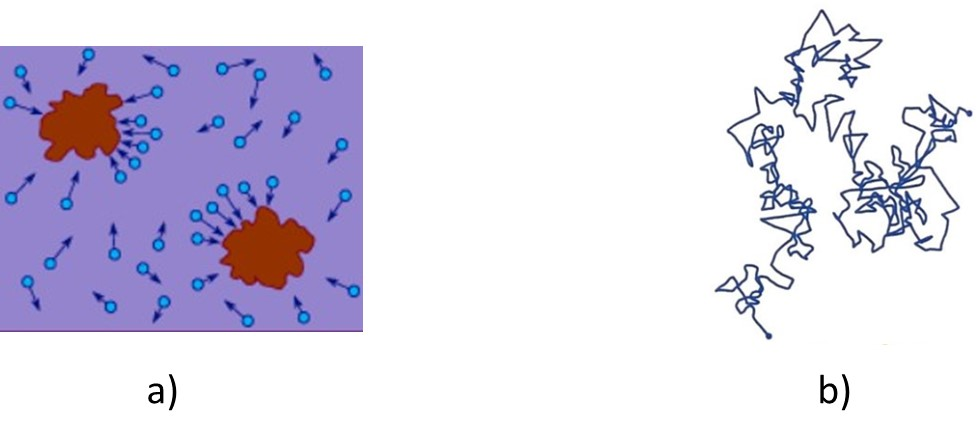
\includegraphics[width=0.5\linewidth]{figs/VN12-Y24-PH-SYL-009-1}
	\captionof{figure}{a) Va chạm của các phân tử nước lên hạt phấn hoa, b) Minh hoạ quỹ đạo gấp khúc của một hạt phấn hoa trong nước. }
\end{center}
\subsubsection{Chất khí}
\paragraph{Tính chất của chất khí}
\begin{boxdn}
	Chất khí có một số tính chất sau:
	\begin{itemize}
		\item Chất khí có hình dạng và thể tích của vật chứa nó.
		\item Chất khí có khối lượng riêng nhỏ hơn nhiều so với chất lỏng và chất rắn.
		\item Chất khí dễ bị nén.
		\item Chất khí gây ra áp suất lên thành bình chứa nó. Khi nhiệt độ tăng, áp suất khí tác dụng lên thành bình tăng.
	\end{itemize}
\end{boxdn}
\paragraph{Lượng chất}
\begin{boxdn}
	Mol là lượng chất trong đó chứa số phân tử (hoặc nguyên tử) bằng 
	$$N_A\approx\SI{6.02E23}{\mole^{-1}}$$
	$N_A$ được gọi là số Avogadro (số phân tử trong 1 mol chất).\\
	Khối lượng mol của một chất là khối lượng của $\SI{1}{\mole}$ chất đó, được kí hiệu là $M$.\\
	Nếu một mẫu chất có khối lượng $m$, chứa $N$ phân tử thì số mol $n$ của mẫu chất đó được xác định:
	$$n=\dfrac{N}{N_A}=\dfrac{m}{M}.$$
\end{boxdn}
\subsubsection{Mô hình động học phân tử chất khí}
\begin{boxdn}
	Nội dung mô hình động học phân tử chất khí gồm các ý chính như sau:
	\begin{itemize}
		\item Chất khí gồm tập hợp rất nhiều các phân tử có kích thước rất nhỏ so với khoảng cách trung bình giữa chúng.
		\item Các phân tử khí luôn chuyển động hỗn loạn, không ngừng và được gọi là chuyển động nhiệt. Nhiệt độ càng cao, các phân tử khí chuyển động càng nhanh.
		\item Trong quá trình chuyển động, các phân tử khí va chạm với thành bình chứa, gây ra áp suất lên thành bình.
	\end{itemize}
\end{boxdn}
\begin{center}
	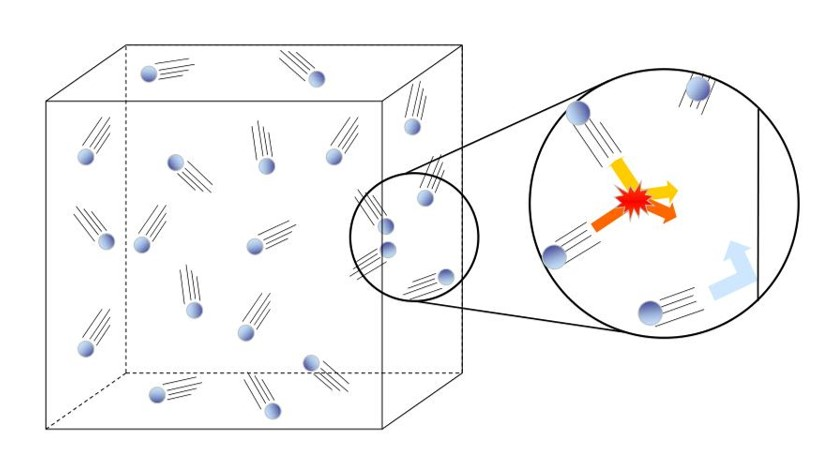
\includegraphics[width=0.4\linewidth]{figs/VN12-Y24-PH-SYL-009-2}
	\captionof{figure}{Các phân tử va chạm vào nhau và va chạm vào thành bình trong quá trình chuyển động nhiệt.}
\end{center}
\subsubsection{Khí lí tưởng}
\begin{boxdn}
	Khí lí tưởng có các đặc điểm sau:
	\begin{enumerate}[label=\arabic*.]
		\item Các phân tử khí được coi là các \textit{chất điểm}, không tương tác với nhau khi chưa va chạm.
		\item Các phân tử khí tương tác khi va chạm với nhau và va chạm với thành bình. Các va chạm này là va chạm \textit{hoàn toàn đàn hồi}.
	\end{enumerate}
\end{boxdn}
\begin{luuy}
	Mô hình khí lí tưởng đơn giản hơn khí thực (khí tồn tại trong thực tế) nhưng vẫn phản ánh được các đặc điểm cơ bản của khí này.
\end{luuy}
\subsection{VÍ DỤ MINH HOẠ}
\begin{dang}{Phân tích mô hình Brown, nêu được các phân tử trong chất khí chuyển động hỗn loạn.}
	\end{dang}
	\begin{vd}
Khi quan sát tia nắng mặt trời chiếu qua cửa sổ vào trong phòng, ta có thể thấy các hạt bụi trong ánh nắng chuyển động không ngừng. Chuyển động này có phải là chuyển động Brown không? Tại sao?
	\loigiai{Chuyển động của các hạt bụi trong trường hợp này không thể coi là chuyển động Brown vì chuyển động chủ yếu của các hạt bụi lúc bấy giờ là chuyển động theo dòng khí do hiện tượng đối lưu.
			}
	\end{vd}

\begin{dang}{Vận dụng được thuyết động học phân tử chất khí}
\end{dang}
\begin{vd}
Trong quá trình bơm xe đạp, khi lốp xe đã gần căng, càng về cuối của mỗi lần bơm thì ta càng thấy khó nén piston xuống. Hãy giải thích hiện tượng trên.
\loigiai{Càng về cuối quá trình bơm săm xe đạp, săm xe đã căng và khó tăng thể tích chứa khí bên trong. Trong khi đó, sau mỗi lần bơm thì số phân tử khí bên trong săm tăng lên đáng kể và làm tăng mật độ phân tử khí bên trong. \\
		Theo thuyết động học phân tử chất khí, khi mật độ phân tử khí bên trong săm tăng thì số va chạm của các phân tử khí lên thành săm và piston tăng. Do đó, áp suất khí tác động lên piston tăng và làm cho piston khó nén xuống hơn.
	}

\end{vd}
% ==================================================================
\begin{vd}
Một phân tử oxygen đang chuyển động qua tâm một bình cầu có đường kính $\SI{0.20}{\meter}$. Tốc độ của phân tử là $\SI{400}{\meter/\second}$. Ước tính số lần phân tử này va chạm vào thành bình chứa trong mỗi giây. Coi rằng tốc độ của phân tử là không đổi.
\loigiai{Trong điều kiện lý tưởng, xem như phân tử oxygen chuyển động thẳng và không bị đổi hướng do va chạm với các phân tử khí khác, tốc độ của phân tử là không đổi và va chạm của phân tử khí với thành bình là tuyệt đối đàn hồi. Ban đầu phân tử khí này chuyển động qua tâm bình cầu nên khi chạm vào thành bình, phân tử khí sẽ bật ngược trở lại với tốc độ như cũ và cũng đi qua tâm bình cầu.\\
		Khoảng thời gian giữa 2 lần liên tiếp phân tử khí va chạm với thành bình:
		$$T=\dfrac{2R}{v}=\dfrac{\SI{0.2}{\meter}}{\SI{400}{\meter/\second}}=\SI{5E-4}{\second}.$$
		Số lần phân tử khí này va chạm vào thành bình trong mỗi giây:
		$$f=\dfrac{1}{T}=2000.$$
	}
\end{vd}
\subsection{BÀI TẬP TRẮC NGHIỆM}
\Opensolutionfile{ans}[ans/G12Y24B8TN]
% ===================================================================
\begin{ex}
	Tính chất nào sau đây \textbf{không phải} là tính chất của chất khí?
	\choice
	{\True Có hình dạng và thể tích riêng.}
	{Có các phân tử chuyển động hỗn loạn không ngừng.}
	{Có thể nén được dễ dàng.}
	{Có khối lượng riêng nhỏ hơn so với chất rắn và chất lỏng.}
	\loigiai{}
\end{ex}
% ===================================================================
\begin{ex}
	Chọn phương án \textbf{sai}. Số Avogadro là
	\choice
	{số phân tử (hay nguyên tử) có trong $\SI{22.4}{\text{lít}}$ khí ở điều kiện tiêu chuẩn $\left(\SI{0}{\celsius}, \SI{1}{atm}\right)$.}
	{số phân tử (hay nguyên tử) có trong 1 mol chất.}
	{\True số phân tử (hay nguyên tử) có trong 1 đơn vị khối lượng chất.}
	{số nguyên tử có trong $\SI{12}{\gram}$ $\ce{^{12}C}$.}
	\loigiai{}
\end{ex}
% ===================================================================
\begin{ex}
Gọi $\xsi{M}{(\gram/\mole)}$ là khối lượng mol nguyên tử, $N_\text{A}$ là số Avogadro. Biểu thức xác định số phân tử hay nguyên tử chứa trong $\xsi{m}{(\gram)}$ của chất đó là	
	\choice
	{$N=MmN_\text{A}$.}
	{$N=\dfrac{MN_\text{A}}{m}$.}
	{\True $N=\dfrac{mN_\text{A}}{M}$.}
	{$N=\dfrac{N_\text{A}}{mM}$.}
	\loigiai{}
\end{ex}
% ===================================================================
\begin{ex}
Điền vào chỗ trống.\\
Chất khí trong đó các phân tử được coi là \dots và chỉ tương tác khi \dots được gọi là khí lí tưởng.	
	\choice
	{\True chất điểm; va chạm.}
	{vật rắn; va chạm.}
	{chất điểm; ở gần nhau.}
	{vật rắn; ở gần nhau.}
	\loigiai{}
\end{ex}
% ===================================================================
\begin{ex}
	Nhận xét nào sau đây về các phân tử khí lí tưởng là \textbf{không đúng}?
	\choice
	{Có thể tích riêng không đáng kể.}
	{Có lực tương tác không đáng kể khi không va chạm.}
	{\True Có khối lượng không đáng kể.}
	{Có vận tốc càng lớn khi nhiệt độ phân tử càng cao.}
	\loigiai{}
\end{ex}
% ===================================================================
\begin{ex}
Chọn câu \textbf{sai}. Số Avogadro có giá trị bằng	
	\choice
	{số nguyên tử chứa trong $\SI{4}{\gram}$ helium.}
	{\True số phân tử chứa trong $\SI{16}{\gram}$ oxygen.}
	{số phân tử chứa trong $\SI{18}{\gram}$ nước lỏng.}
	{số nguyên tử chứa trong $\SI{22.4}{\liter}$ khí trơ ở $\SI{0}{\celsius}$ và áp suất $\SI{1}{atm}$.}
	\loigiai{}
\end{ex}
% ===================================================================
\begin{ex}
Một bình kín chứa $N=\SI{3.01E23}{}$ phân tử khí helium. Khối lượng helium chứa trong bình là	
	\choice
	{$\SI{0.5}{\gram}$.}
	{$\SI{1}{\gram}$.}
	{\True $\SI{2}{\gram}$.}
	{$\SI{4}{\gram}$.}
	\loigiai{}
\end{ex}
% ===================================================================
\begin{ex}
	Cho biết khối lượng riêng của không khí ở điều kiện tiêu chuẩn là $\SI{1.29}{\kilogram/\meter^3}$. Coi không khí như một chất khí thuần nhất, khối lượng mol của không khí là
	\choice
	{$\SI{0.041}{\kilogram/\mole}$.}
	{\True $\SI{0.029}{\kilogram/\mole}$.}
	{$\SI{0.023}{\kilogram/\mole}$.}
	{$\SI{0.026}{\kilogram/\mole}$.}
	\loigiai{$$\rho=\dfrac{m}{V}=\dfrac{m}{n\cdot\left(\SI{22.4E-3}{\meter^3}\right)}\Rightarrow M=\dfrac{m}{n}=\SI{0.029}{\kilogram/\mole}.$$}
\end{ex}
\Closesolutionfile{ans}
\subsection{TRẮC NGHIỆM ĐÚNG/SAI}
\setcounter{ex}{0}
% ===================================================================
\begin{ex}
	Nhận định các phát biểu sau về đặc điểm của chuyển động Brown.
	\begin{enumerate}[label=\alph*)]
	\item Chuyển động Brown tuân theo một số quy luật nhất định.
	\item Quỹ đạo của chuyển động Brown là những đường gấp khúc.
	\item Chuyển động Brown là chuyển động của các hạt nhẹ trong chất rắn, lỏng, khí.
	\item Nhiệt độ càng cao thì các phân tử khí chuyển động càng hỗn loạn.
\end{enumerate}
	\loigiai{\begin{enumerate}[label=\alph*)]
			\item Sai. Chuyển động Brown không theo quy luật.
			\item Đúng.
			\item Sai. Chuyển động Brown là chuyển động của các hạt nhẹ trong chất lỏng và chất khí.
			\item Đúng.
		\end{enumerate}
	}
\end{ex}
% ===================================================================
\begin{ex}
	Nhận định các phát biểu sau về nội dung thuyết động học phân tử chất khí.
	\begin{enumerate}[label=\alph*)]
		\item Chất khí gồm tập hợp nhiều các phân tử dao động nhiệt quanh các vị trí cân bằng của chúng.
		\item Nhiệt độ càng cao thì các phân tử khí chuyển động nhiệt càng nhanh.
		\item Kích thước các phân tử rất nhỏ so với khoảng cách trung bình giữa chúng.
		\item Áp suất khí được tạo ra bởi sự va chạm giữa các phân tử khí với nhau.
	\end{enumerate}
	\loigiai{\begin{enumerate}[label=\alph*)]
			\item Sai. Các phân tử khí chuyển động hỗn loạn, không ngừng.
			\item Đúng.
			\item Đúng.
			\item Sai. Sự va chạm của các phân tử khí với thành bình gây ra áp suất lên thành bình.
		\end{enumerate}
	}
\end{ex}
% ===================================================================
\begin{ex}
	Nhận định các phát biểu sau đây về đặc điểm của khí lí tưởng
	\begin{enumerate}[label=\alph*)]
		\item Các phân tử khí được coi là chất điểm nên người ta có thể bỏ qua khối lượng các phân tử khí.
		\item Thể tích khối khí bằng thể tích bình chứa trừ đi thể tích riêng của các phân tử.
		\item Các phân tử khí chỉ tương tác với nhau khi va chạm.
		\item Nội năng của khối khí bằng tổng động năng chuyển động nhiệt của các phân tử khí và chỉ phụ thuộc vào nhiệt độ.
	\end{enumerate}
	
	\loigiai{\begin{enumerate}[label=\alph*)]
			\item Sai. Các phân tử khí được coi là chất điểm nên người ta có thể bỏ qua kích thước các phân tử khí.
			\item Sai. Thể tích khối khí bằng thể tích bình chứa.
			\item Đúng.
			\item Đúng.
		\end{enumerate}
	}
\end{ex}
% ===================================================================
\begin{ex}
	Một người xịt nước hoa ở đầu phòng thì người ở cuối phòng vẫn nghe được mùi hương của nước hoa.
	\begin{enumerate}[label=\alph*)]
		\item Hiện tượng trên được gọi là sự khuếch tán.
		\item Các phân tử nước hoa chuyển động thành dòng từ đầu phòng sang cuối phòng chỉ nhờ vào đối lưu.
		\item Hiện tượng trên chứng tỏ nhiệt độ ở đầu phòng cao hơn nhiệt độ ở cuối phòng.
		\item Nhiệt độ trong phòng càng cao thì người ở cuối phòng càng sớm nhận ra mùi nước hoa.
	\end{enumerate}
	
	\loigiai{\begin{enumerate}[label=\alph*)]
			\item Đúng.
			\item Sai. Sự dao động nhiệt của các phân tử khí và phân tử nước hoa làm cho chúng khuếch tán vào nhau.
			\item Sai. Các phân tử khí chuyển động hỗn loạn, không ngừng về mọi phía nên không thể khẳng định được nhiệt độ nơi nào cao hơn.
			\item Đúng. Nhiệt độ càng cao, các phân tử chuyển động càng nhanh làm tốc độ khuếch tán diễn ra càng nhanh.
		\end{enumerate}
	}
\end{ex}
\subsection{BÀI TẬP TỰ LUẬN}
\setcounter{ex}{0}
% ===================================================================
\begin{ex}
	Mùi hôi từ các bãi rác thải là một vấn nạn đối với cư dân sống xung quanh. Khi thời tiết càng nắng nóng thì mùi hôi bốc ra càng nồng nặc và càng bay xa (ngay cả trong điều kiện không có gió). Dựa vào thuyết động học phân tử chất khí, hãy giải thích điều này và đề xuất biện pháp hạn chế tình trạng trên.
	\loigiai{Thời tiết càng nóng thì quá trình phân huỷ các chất hữu cơ diễn ra càng nhanh và sinh ra nhiều khí có mùi hôi như: $\ce{H_2S}, \ce{NH_3}, \ce{CH_4}, \ce{SO_2},\dots$. Bên cạnh đó, nhiệt độ càng cao thì các phân tử khí chuyển động nhiệt càng nhanh, do đó các phân tử khí này càng dễ khuếch tán vào không khí và bay đi xa hơn.\\
		Biện pháp hạn chế: Thường xuyên thu gom, xử lý rác thải, nâng cao ý thức cộng đồng.
	}
\end{ex}
% ===================================================================
\begin{ex}
Đun một nồi nước trên bếp, khi nước sôi nắp nồi thường bị đẩy lên. Hãy giải thích điều này.
	
	\loigiai{Khi đun nước đến nhiệt độ sôi, nước sẽ bay hơi tạo thành hơi nước. Bên cạnh đó, nhiệt độ càng cao làm cho các phân tử khí và hơi nước trong nồi chuyển động càng nhanh. Sự gia tăng mật độ khí và tốc độ chuyển động nhiệt của các phân tử khí và hơi nước trong nồi làm gia tăng số lượt va chạm của các phân tử khí lên nắp nồi $\rightarrow$ tăng áp suất khí tác dụng lên nắp và làm nắp bị đẩy lên.
	}
\end{ex}
% ===================================================================
\begin{ex}
	Xác định số phân tử chứa trong
	\begin{enumerate}[label=\alph*)]
		\item $\SI{0.2}{\kilogram}$ nước.
		\item $\SI{1}{\kilogram}$ không khí nếu như không khí có $\SI{22}{\percent}$ là khí $\ce{O_2}$ và $\SI{78}{\percent}$ là khí $\ce{N_2}$.
	\end{enumerate}
	\loigiai{\begin{enumerate}[label=\alph*)]
			\item $N=\dfrac{m}{M_{\ce{H_2O}}}\cdot N_\text{A}\approx\SI{6.68E24}{\text{phân tử}}.$
			\item $N=\SI{22}{\percent}\cdot\dfrac{m}{M_{\ce{O_2}}}\cdot N_\text{A}+\SI{78}{\percent}\cdot\dfrac{m}{M_{\ce{N_2}}}\cdot N_\text{A}\approx\SI{2.1E25}{\text{phân tử}}.$
		\end{enumerate}
	}
\end{ex}
% ===================================================================
\begin{ex}
	Coi Trái Đất là một khối cầu bán kính $\SI{6400}{\kilo\meter}$, nếu lấy toàn bộ số phân tử nước trong $\SI{1.0}{\gram}$ hơi nước trải đều trên bề mặt Trái Đất thì mỗi mét vuông trên bề mặt Trái Đất có bao nhiêu phân tử nước? Biết khối lượng mol của phân tử nước khoảng $\SI{18}{\gram/\mole}$.
	\loigiai{$$\eta=\dfrac{N}{S}=\dfrac{\dfrac{m}{M}N_\text{A}}{4\pi R^2}=\SI{64.98E6}{\text{phân tử}/\meter^2}.$$}
\end{ex}	
%\newpage\section{ĐỊNH LUẬT BOYLE}
\subsection{LÝ THUYẾT TRỌNG TÂM}
\subsubsection{Trạng thái và quá trình biến đổi trạng thái}
\begin{boxdn}
	\textbf{Trạng thái của một khối khí } được xác định bằng ba thông số, gọi là thông số trạng thái của khối khí: thể tích $V$, áp suất $p$ và nhiệt độ tuyệt đối $T$. Giữa các thông số trạng thái của một khối khí xác định có những mối liên hệ mang tính quy luật.
\end{boxdn}
\begin{center}
	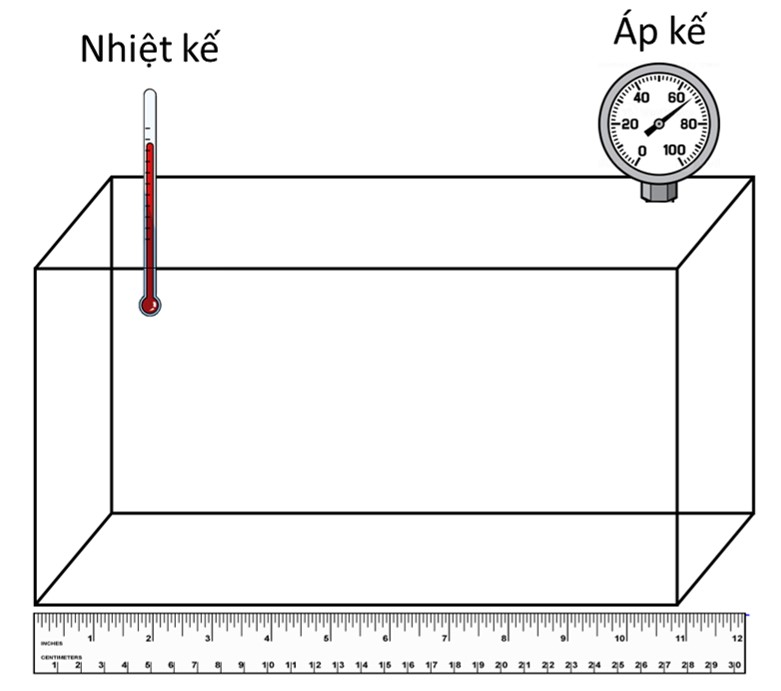
\includegraphics[width=0.35\linewidth]{figs/VN12-Y24-PH-SYL-010-1}
	\captionof{figure}{Xác định các thông số trạng thái của một lượng khí}
\end{center}
\begin{boxdn}
	\textbf{Quá trình biến đổi trạng thái là} quá trình khối khí biến đổi từ trạng thái này sang trạng thái khác.\\
	\textbf{Đẳng quá trình} là quá trình biến đổi trạng thái mà trong đó có một thông số trạng thái được giữ không đổi.\\
	Các đẳng quá trình:
	\begin{itemize}
		\item Đẳng nhiệt là quá trình biến đổi trạng thái của một khối khí xác định, trong đó nhiệt độ được giữ không đổi.
		\item Đẳng áp là quá trình biến đổi trạng thái của một khối khí xác định, trong đó áp suất được giữ không đổi.
		\item Đẳng tích là quá trình biến đổi trạng thái của một khối khí xác định, trong đó thể tích được giữ không đổi.
	\end{itemize}
\end{boxdn}
\begin{luuy}
	Vì chất khí luôn chiếm toàn bộ dung tích của bình chứa nên thể tích của một lượng khí bằng dung tích bình chứa nó.
\end{luuy}
\subsubsection{Định luật Boyle}
\begin{boxdl}
	Ở nhiệt độ không đổi, áp suất của một khối khí xác định tỉ lệ nghịch với thể tích của nó.
	\begin{equation}
		pV=\text{hằng số}
	\end{equation}
\end{boxdl}
Đường biểu diễn sự phụ thuộc của $p$ theo $V$ khi nhiệt độ của khối khí không đổi gọi là \textbf{đường đẳng nhiệt}.
\begin{center}
	\begin{tikzpicture}  
		\begin{axis}[  ultra thick,
			xmin=0,  
			xmax=24,  
			xtick=\empty,
			ytick=\empty,
			ymin=0,  
			ymax=5.8, 
			samples=300,
			xticklabels=\empty,
			yticklabels=\empty,
			axis lines=center, 
			xlabel=$V$, 
			ylabel=$p$, 
			every axis y label/.style={at=(current axis.above origin),anchor=south},  
			every axis x label/.style={at=(current axis.right of origin),anchor=west},  ]
			\addplot [ultra thick, blue, smooth, domain=1:20] {5/x} node[right] {$T_1$}; 
			\addplot [ultra thick, red, smooth, domain=3:20] {15/x} node[right] {$T_2$}; 
		\end{axis}  
		\node[label={[below left]90:O}] at (0,0){};
	\end{tikzpicture}
	\captionof{figure}{Các đường đẳng nhiệt của một khối khí lí tưởng tương ứng với nhiệt độ $T_1$ và $T_2\left(T_2>T_1\right)$}
	
\end{center}
\subsection{Mục tiêu bài học - Ví dụ minh hoạ}
\begin{dang}{Vận dụng định luật Boyle giải thích được một số hiện tượng trong thực tế}
	\end{dang}
\begin{vd}
Nếu lật úp một chiếc cốc thuỷ tinh rồi nhúng chìm chiếc cốc vào trong nước thì thể tích phần không khí bị giam trong cốc sẽ thay đổi như thế nào trong quá trình chiếc cốc chìm sâu xuống nước?
\loigiai{
			Trong quá trình cốc chìm xuống nước thì nhiệt độ không khí trong cốc không thay đổi. Cốc càng chìm sâu vào trong nước thì áp suất của không khí trong cốc càng tăng. Theo định luật Boyle, khi đó thể tích của không khí bị giam trong cốc ngày càng giảm.
}
\end{vd}
% ======================================================
\begin{vd}
Để đưa thuốc từ lọ vào trong cylanh của ống tiêm, ban đầu nhân viên y tế đẩy piston sát đáy cylanh, sau đó đưa đầu kim tiêm (được gắn với ống tiêm) vào trong lọ thuốc. Khi kéo piston, thuốc sẽ chảy vào trong cylanh. Em hãy giải thích cơ sở khoa học của việc làm trên?
	\begin{center}
		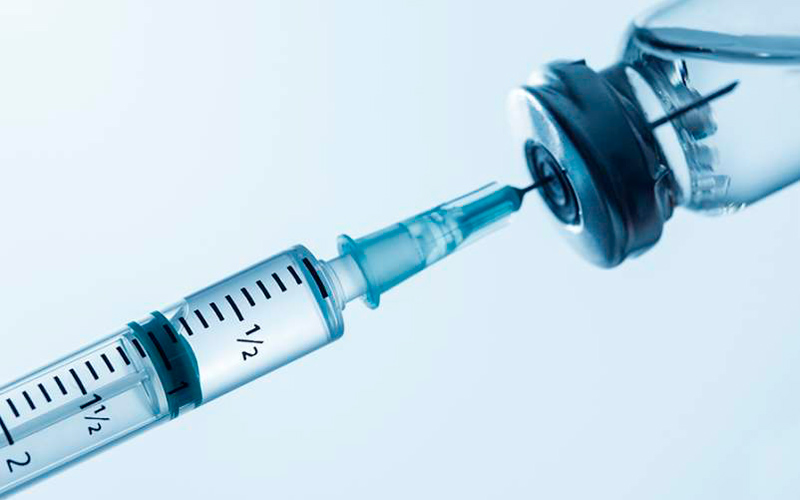
\includegraphics[width=0.35\linewidth]{figs/VN12-Y24-PH-SYL-010-2}
	\end{center}
\loigiai{
		Khi mới đưa đầu kim tiêm vào trong lọ thuốc, áp suất khí còn lại trong cylanh bằng áp suất chất lỏng trong lo thuốc. Khi kéo piston, thể tích khí trong cylanh tăng (nhiệt độ khí gần như không đổi). Theo định luật Boyle, áp suất khí trong cylanh giảm và nhỏ hơn áp suất chất lỏng trong lọ. Do đó, chất lỏng trong lọ bị đẩy qua kim và chảy sang cylanh cho đến khi có sự cân bằng áp suất ở cả hai phía.
	}
\end{vd}

\begin{dang}{Giải được các bài toán liên quan quá trình đẳng nhiệt}
\end{dang}
\begin{vd}
Một lượng khí có thể tích $\SI{10}{\text{lít}}$ ở áp suất $\SI{E5}{\pascal}$. Tính thể tích của lượng khí này ở áp suất $\SI{1.25E5}{\pascal}$. Biết nhiệt độ của khí không đổi.
\loigiai{
		\begin{center}
			\begin{tabular}{C{4cm} C{3cm} C{4cm}}
				\colorbox{yellow}{\textcolor{red}{\textbf{Trạng thái 1}}} & $\xrightarrow[]{T_1=T_2}$ & \colorbox{yellow}{\textcolor{red}{\textbf{Trạng thái 2}}}\\
				$p_1=\SI{E5}{\pascal}$ & &$p_2=\SI{1.25E5}{\pascal}$\\
				$V_1=\SI{10}{\text{lít}}$ & & $V_2=?$
			\end{tabular}
		\end{center}
		Theo định luật Boyle:
		$$p_1V_1=p_2V_2\Rightarrow V_2=\dfrac{p_1V_1}{p_2}=\dfrac{\left(\SI{E5}{\pascal}\right)\cdot\left(\SI{10}{\text{lít}}\right)}{\SI{1.25E5}{\pascal}}=\SI{8}{\text{lít}}.$$
		Vậy: ở áp suất $\SI{1.25E5}{\pascal}$ thì thể tích bọt khí là $\SI{8}{\text{lít}}$.
}
\end{vd}
% ===============================================================	
\begin{vd}
Một bọt khí nổi lên từ đáy giếng sâu $\SI{6}{\meter}$ lên mặt nước. Khi lên tới mặt nước, thể tích của bọt khí tăng lên bao nhiêu lần? Coi áp suất khí quyển là $\SI{1.013E5}{\pascal}$; khối lượng riêng của nước giếng là $\SI{1003}{\kilogram/\meter^3}$ và nhiệt độ của nước giếng không thay đổi theo độ sâu. Lấy gia tốc trọng trường $g=\SI{9.81}{\meter/\second^2}$.
\loigiai{
		Áp suất trong bọt khí khi ở độ sâu $\SI{6}{\meter}$ so với mặt nước:
		$$p_1=p_0+\rho gh=\SI{1.013E5}{\pascal}+\left(\SI{1003}{\kilogram/\meter^3}\right)\cdot\left(\SI{9.81}{\meter
			/\second^2}\right)\cdot\left(\SI{6}{\meter}\right)\approx\SI{1.6E5}{\pascal}$$
		\begin{center}
			\begin{tabular}{C{4cm} C{3cm} C{4cm}}
				\colorbox{yellow}{\textcolor{red}{\textbf{Trạng thái 1}}} & $\xrightarrow[]{T_1=T_2}$ & \colorbox{yellow}{\textcolor{red}{\textbf{Trạng thái 2}}}\\
				$p_1=\SI{1.6E5}{\pascal}$ & &$p_2=p_0=\SI{1.013E5}{\pascal}$\\
				$V_1$ & & $V_2$
			\end{tabular}
		\end{center}
		Theo định luật Boyle:
		$$p_1V_1=p_2V_2\Rightarrow \dfrac{V_2}{V_1}=\dfrac{p_1}{p_2}=\dfrac{\SI{1.6E5}{\pascal}}{\SI{1.013E5}{\pascal}}\approx1,58.$$
		Vậy: khi nổi lên mặt nước, thể tích bọt khí đã tăng lên 1,58 lần.
}
\end{vd}
% ==============================================================
\begin{vd}
	Một cột không khí chứa trong một ống nhỏ, dài, tiết diện đều, ban đầu ống được đặt nằm ngang (như hình). Cột không khí được ngăn cách bởi một cột thuỷ ngân có chiều dài $d=\SI{150}{\milli\meter}$. Áp suất khí quyển là $p_0=\SI{750}{\milli\meter Hg}$. Biết chiều dài ban đầu của cột không khí là $\ell_0=\SI{144}{\milli\meter}$.
		\begin{center}
			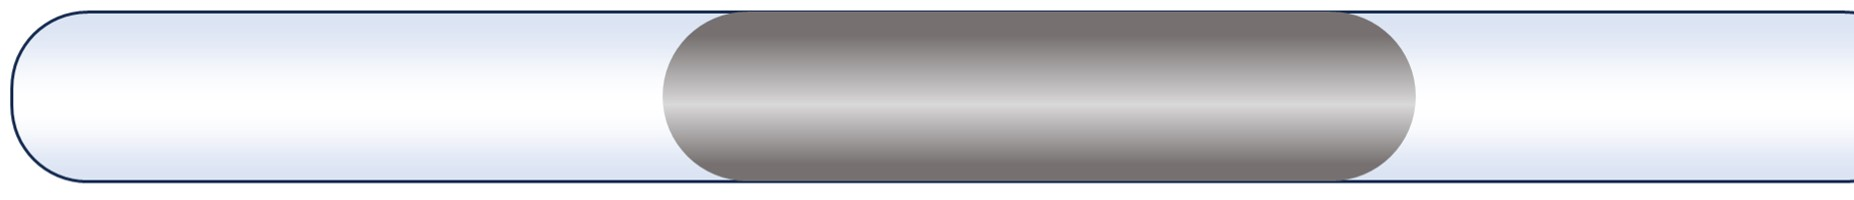
\includegraphics[width=0.4\linewidth]{figs/VN12-Y24-PH-SYL-010-3}
		\end{center}
		Hãy tính chiều dài cột không khí nếu:
		\begin{enumerate}[label=\alph*)]
			\item ống thẳng đứng, miệng ống ở trên.
			\item ống thẳng đứng, miệng ống ở dưới.
			\item ống đặt nghiêng góc $\alpha=\SI{30}{\degree}$ so với phương ngang, miệng ống ở dưới.
			\item ống đặt nghiêng góc $\alpha=\SI{30}{\degree}$ so với phương ngang, miệng ống ở trên.
		\end{enumerate}
		Giả sử ống đủ dài để cột thuỷ ngân luôn ở trong ống và nhiệt độ là không đổi.
	\loigiai{Gọi $S$ là tiết diện của ống.
			\begin{enumerate}[label=\alph*)]
				\item Trường hợp ống đặt thẳng đứng, miệng ống hướng lên:\\
				\begin{minipage}[l]{0.25\textwidth}
					\begin{center}
						
\includegraphics[width=0.1\linewidth]{figs/VN12-Y24-PH-SYL-010-4}
					\end{center}
				\end{minipage}
				\begin{minipage}[l]{0.75\textwidth}
					\begin{center}
						\begin{tabular}{C{4cm} C{2cm} C{4cm}}
							\colorbox{yellow}{\textcolor{red}{\textbf{Trạng thái ban đầu}}} & $\xrightarrow[]{T=const}$ & \colorbox{yellow}{\textcolor{red}{\textbf{Trạng thái câu a}}}\\
							$p_0=\SI{750}{\milli\meter Hg}$ & &$p_a=p_0+d=\SI{900}{\milli\meter Hg}$\\
							$V_0=\ell_0S$ & & $V_a=\ell_a S$
						\end{tabular}
					\end{center}
					Theo định luật Boyle:
					$$p_0V_0=p_aV_a$$
					$$\Leftrightarrow p_0\ell_0S=p_a\ell_aS$$
					$$\Rightarrow \ell_a=\dfrac{p_0\ell_0}{p_a}=\dfrac{\left(\SI{750}{\milli\meter Hg}\right)\cdot\left(\SI{144}{\milli\meter}\right)}{\SI{900}{\milli\meter Hg}}=\SI{120}{\milli\meter}.$$
				\end{minipage}
				\item Trường hợp ống đặt thẳng đứng, miệng ống hướng xuống:\\
				\begin{minipage}[l]{0.25\textwidth}
					\begin{center}
						
\includegraphics[width=0.1\linewidth]{figs/VN12-Y24-PH-SYL-010-5}
					\end{center}
				\end{minipage}
				\begin{minipage}[l]{0.75\textwidth}
					\begin{center}
						\begin{tabular}{C{4cm} C{2cm} C{4cm}}
							\colorbox{yellow}{\textcolor{red}{\textbf{Trạng thái ban đầu}}} & $\xrightarrow[]{T=const}$ & \colorbox{yellow}{\textcolor{red}{\textbf{Trạng thái câu b}}}\\
							$p_0=\SI{750}{\milli\meter Hg}$ & &$p_b=p_0-d=\SI{600}{\milli\meter Hg}$\\
							$V_0=\ell_0S$ & & $V_b=\ell_b S$
						\end{tabular}
					\end{center}
					Theo định luật Boyle:
					$$p_0V_0=p_bV_b$$
					$$\Leftrightarrow p_0\ell_0S=p_b\ell_bS$$
					$$\Rightarrow \ell_b=\dfrac{p_0\ell_0}{p_b}=\dfrac{\left(\SI{750}{\milli\meter Hg}\right)\cdot\left(\SI{144}{\milli\meter}\right)}{\SI{600}{\milli\meter Hg}}=\SI{180}{\milli\meter}.$$
				\end{minipage}
				\item Trường hợp ống đặt nghiêng góc $\alpha=\SI{30}{\degree}$ so với phương ngang, miệng ống ở dưới:\\
				\begin{minipage}[l]{0.25\textwidth}
					\begin{center}
						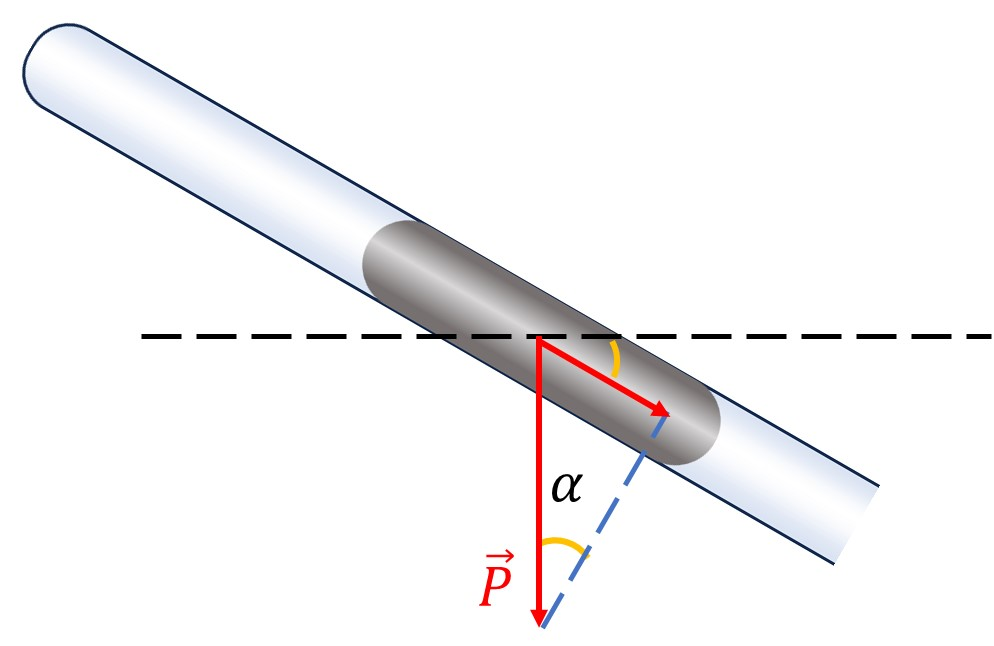
\includegraphics[width=1.0\linewidth]{figs/VN12-Y24-PH-SYL-010-6}
					\end{center}
				\end{minipage}
				\begin{minipage}[l]{0.75\textwidth}
					\begin{center}
						\begin{tabular}{C{4cm} C{1.5cm} C{4.5cm}}
							\colorbox{yellow}{\textcolor{red}{\textbf{Trạng thái ban đầu}}} & $\xrightarrow[]{T=const}$ & \colorbox{yellow}{\textcolor{red}{\textbf{Trạng thái câu c}}}\\
							$p_0=\SI{750}{\milli\meter Hg}$ & &$p_c=p_0-d\sin\alpha=\SI{675}{\milli\meter Hg}$\\
							$V_0=\ell_0S$ & & $V_c=\ell_c S$
						\end{tabular}
					\end{center}
					Theo định luật Boyle:
					$$p_0V_0=p_cV_c$$
					$$\Leftrightarrow p_0\ell_0S=p_c\ell_cS$$
					$$\Rightarrow \ell_c=\dfrac{p_0\ell_0}{p_c}=\dfrac{\left(\SI{750}{\milli\meter Hg}\right)\cdot\left(\SI{144}{\milli\meter}\right)}{\SI{675}{\milli\meter Hg}}=\SI{160}{\milli\meter}.$$
				\end{minipage}
				\item Trường hợp ống đặt nghiêng góc $\alpha=\SI{30}{\degree}$ so với phương ngang, miệng ống ở trên:\\
				\begin{minipage}[l]{0.25\textwidth}
					\begin{center}
						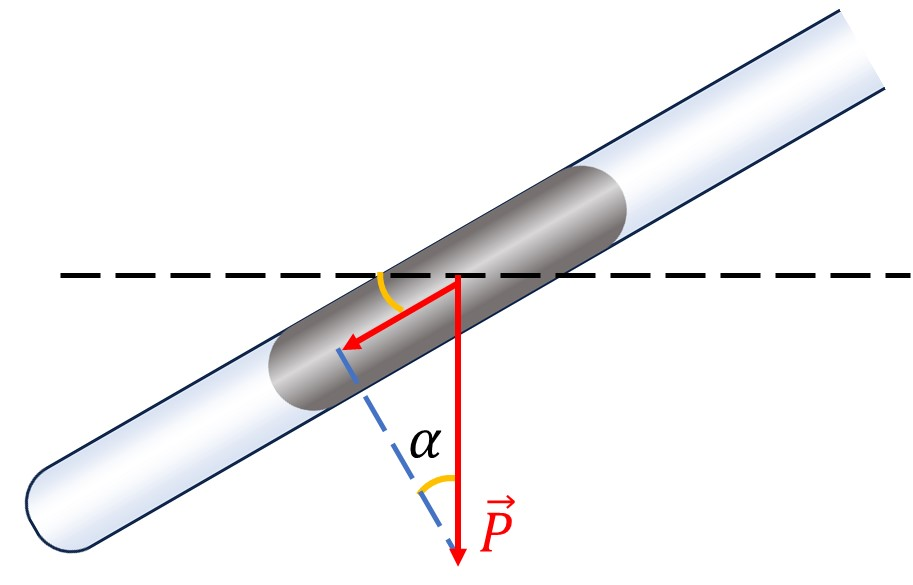
\includegraphics[width=1.0\linewidth]{figs/VN12-Y24-PH-SYL-010-7}
					\end{center}
				\end{minipage}
				\begin{minipage}[l]{0.75\textwidth}
					\begin{center}
						\begin{tabular}{C{4cm} C{1.5cm} C{4.5cm}}
							\colorbox{yellow}{\textcolor{red}{\textbf{Trạng thái ban đầu}}} & $\xrightarrow[]{T=const}$ & \colorbox{yellow}{\textcolor{red}{\textbf{Trạng thái câu d}}}\\
							$p_0=\SI{750}{\milli\meter Hg}$ & &$p_d=p_0+d\sin\alpha=\SI{825}{\milli\meter Hg}$\\
							$V_0=\ell_0S$ & & $V_d=\ell_d S$
						\end{tabular}
					\end{center}
					Theo định luật Boyle:
					$$p_0V_0=p_dV_d$$
					$$\Leftrightarrow p_0\ell_0S=p_d\ell_dS$$
					$$\Rightarrow \ell_d=\dfrac{p_0\ell_0}{p_d}=\dfrac{\left(\SI{750}{\milli\meter Hg}\right)\cdot\left(\SI{144}{\milli\meter}\right)}{\SI{825}{\milli\meter Hg}}\approx\SI{131}{\milli\meter}.$$
				\end{minipage}
			\end{enumerate}
	}
\end{vd}
\begin{dang}{Giải được bài toán piston cân bằng}
	\end{dang}
\begin{vd}
	Một lượng không khí có thể tích $\SI{240}{\centi\meter^3}$ chứa trong một cylanh có piston đóng kín, tiết diện của piston là $\SI{24}{\centi\meter^2}$. Áp suất của không khí trong cylanh bằng áp suất không khí bên ngoài là $\SI{E5}{\pascal}$. Cần một lực tối thiểu bằng bao nhiêu để dịch chuyển piston một đoạn $\SI{2}{\centi\meter}$ theo chiều làm thể tích khí giảm? Bỏ qua ma sát giữa giữa piston và thành cylanh. Coi trong quá trình piston chuyển động thì nhiệt độ của không khí không thay đổi.
	\begin{center}
		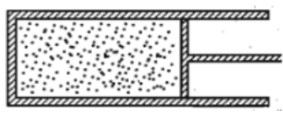
\includegraphics[width=0.25\linewidth]{figs/VN12-Y24-PH-SYL-010-8}
	\end{center}
\loigiai{
	\begin{center}
		\begin{tabular}{C{6cm} C{2cm} C{7cm}}
			\colorbox{yellow}{\textcolor{red}{\textbf{Trạng thái 1}}} & $\xrightarrow[]{T_1=T_2}$ & \colorbox{yellow}{\textcolor{red}{\textbf{Trạng thái 2}}}\\
			$p_1=\SI{E5}{\pascal}$ & &$p_2=?$\\
			$V_1=\SI{240}{\centi\meter^3}$ & & $V_2=\SI{240}{\centi\meter^3}-\left(\SI{24}{\centi\meter^2}\right)\cdot\left(\SI{2}{\centi\meter}\right)=\SI{192}{\centi\meter^3}$
		\end{tabular}
	\end{center}
	Theo định luật Boyle:
	$$p_1V_1=p_2V_2\Rightarrow p_2=\dfrac{p_1V_1}{V_2}=\dfrac{\left(\SI{100}{\kilo\pascal}\right)\cdot\left(\SI{240}{\centi\meter^3}\right)}{\SI{192}{\centi\meter^3}}=\SI{125}{\kilo\pascal}.$$
	\begin{center}
		\includegraphics[width=0.25\linewidth]{figs/VN12-Y24-PH-SYL-010-9}
	\end{center}
	Piston cân bằng khi:
	$$p_2S=p_0S+F\Rightarrow F=\left(p_2-p_0\right)S=\left(\SI{125E3}{\pascal}-\SI{100E3}{\pascal}\right)\cdot\left(\SI{24E-4}{\meter^2}\right)=\SI{60}{\newton}.$$
}
\end{vd}
% ===============================================================
\begin{vd}
	Một bình hình trụ kín hai đầu có độ cao $h=\SI{40}{\centi\meter}$, được đặt nằm ngang, bên trong có một piston rất mỏng và có thể dịch chuyển không ma sát trong bình. Lúc đầu piston được giữ cố định ở chính giữa bình. Hai bên piston chứa cùng loại khí nhưng áp suất khí bên trái $\left(p_1\right)$ lớn gấp 3 lần áp suất khí chứa ở bên phải $\left(p_2\right)$. Piston và thành bình đều được làm từ vật liệu cách nhiệt. Khi thả để piston di chuyển tự do thì piston sẽ di chuyển một đoạn bao nhiêu, theo chiều nào?
		\begin{center}
			\includegraphics[width=0.25\linewidth]{figs/VN12-Y24-PH-SYL-010-10}
		\end{center}
\loigiai{
			Vì áp suất khí bên trái lớn hơn áp suất khí bên phải nên khi được thả tự do piston sẽ di chuyển theo chiều từ trái sang phải.\\
			Piston di chuyển đến khi áp suất khí hai bên piston cân bằng. Gọi:
			\begin{itemize}
				\item $p$ là áp suất khí mỗi bên khi piston đạt trạng thái cân bằng;
				\item $x$ là độ dời của piston.
			\end{itemize}
			Áp dụng định luật Boyle cho khí ở mỗi vách ngăn khi vừa thả piston và khi piston cân bằng:
			$$pV=\text{const}\Rightarrow \begin{cases}
				p_1\cdot\dfrac{hS}{2}=p\left(\dfrac{h}{2}+x\right)S\\
				p_2\cdot\dfrac{hS}{2}=p\left(\dfrac{h}{2}-x\right)S\\
			\end{cases}\Rightarrow \dfrac{p_1}{p_2}=\dfrac{\SI{20}{\centi\meter}+x}{\SI{20}{\centi\meter}-x}=3\Rightarrow x=\SI{10}{\centi\meter}.$$
			
	}
\end{vd}
\subsection{BÀI TẬP TRẮC NGHIỆM}
\Opensolutionfile{ans}[ans/G12Y24B9TN]
% ===================================================================
\begin{ex}
	Tập hợp ba thông số xác định trạng thái của một lượng khí xác định là
	\choice
	{áp suất, thể tích, khối lượng}
	{\True áp suất, nhiệt độ, thể tích}
	{thể tích, trọng lượng, áp suất}
	{áp suất, nhiệt độ, số mol}
	\loigiai{}
\end{ex}
% ===================================================================
\begin{ex}
	Quá trình đẳng nhiệt là
	
	\choice
	{quá trình biến đổi trạng thái của một lượng khí xác định trong đó áp suất được giữ không đổi}
	{quá trình biến đổi trạng thái của một lượng khí xác định trong đó nội năng của khí không đổi}
	{\True quá trình biến đổi trạng thái của một lượng khí xác định trong đó nhiệt độ được giữ không đổi}
	{quá trình biến đổi trạng thái của một lượng khí xác định trong đó thể tích được giữ không đổi}
	\loigiai{}
\end{ex}
% ===================================================================
\begin{ex}
	Trong các hệ thức sau đây, hệ thức nào \textbf{không phù hợp} với định luật Boyle?
	\choice
	{$p\sim\dfrac{1}{V}$}
	{$pV=\text{const}$}
	{\True $V\sim p$}
	{$p_1V_1=p_2V_2$}
	\loigiai{}
\end{ex}
% ===================================================================
\begin{ex}
Nhận định nào sau đây là \textbf{sai} khi nói về quá trình đẳng nhiệt?	
	\choice
	{Tích của áp suất và thể tích luôn không đổi}
	{Áp suất và thể tích tỉ lệ nghịch với nhau}
	{Khi áp suất khí tăng 2 lần thì tích $pV$ vẫn không đổi}
	{\True Khi thể tích khí giảm 2 lần thì áp suất khí cũng giảm 2 lần}
	\loigiai{}
\end{ex}
% ===================================================================
\begin{ex}
Đường đẳng nhiệt trong hệ trục toạ độ $pOV$ là
	
	\choice
	{đường thẳng đi qua gốc toạ độ}
	{đường thẳng kéo dài đi qua gốc toạ độ}
	{\True đường cong hyperbol}
	{một nhánh của parabol}
	\loigiai{}
\end{ex}
% ===================================================================
\begin{ex}
	Cho một lượng khí lí tưởng xác định. Nén đẳng nhiệt khối khí từ thể tích $\SI{10}{\liter}$ đến thể tích $\SI{4}{\liter}$ thì áp suất khí
	\choice
	{\True tăng 2,5 lần}
	{giảm 2,5 lần}
	{tăng 6 lần}
	{giảm 6 lần}
	\loigiai{$$p_1V_1=p_2V_2\Rightarrow\dfrac{p_2}{p_1}=\dfrac{V_1}{V_2}=2,5.$$
	}
\end{ex}
% ===================================================================
\begin{ex}
	Một lượng khí lí tưởng xác định dãn nở đẳng nhiệt từ thể tích $\SI{2}{\liter}$ đến $\SI{8}{\liter}$, ban đầu áp suất khí là $\SI{8E5}{\pascal}$. Trong quá trình trên thì áp suất khí
	\choice
	{tăng $\SI{6E5}{\pascal}$}
	{tăng $\SI{2E5}{\pascal}$}
	{giảm $\SI{2E5}{\pascal}$}
	{\True giảm $\SI{6E5}{\pascal}$}
	\loigiai{$$p_2=\dfrac{p_1V_1}{V_2}=\SI{2E5}{\pascal}\Rightarrow \Delta p=p_2-p_1=\SI{-6E5}{\pascal}.$$
	}
\end{ex}
% ===================================================================
\begin{ex}
	Nén đẳng nhiệt một khối khí lí tưởng xác định làm áp suất khí thay đổi một lượng $\SI{0.5}{atm}$. Biết thể tích và áp suất ban đầu của khối khí là $\SI{5}{\liter}$ và $\SI{2}{atm}$. Thể tích của khối khí lúc sau là
	\choice
	{$\SI{6.25}{\liter}$}
	{\True $\SI{4}{\liter}$}
	{$\SI{6.67}{\liter}$}
	{$\SI{20}{\liter}$}
	\loigiai{\begin{center}
			\begin{tabular}{C{4cm} C{3cm} C{4cm}}
				\colorbox{yellow}{\textcolor{red}{\textbf{Trạng thái 1}}} & $\xrightarrow[]{T_1=T_2}$ & \colorbox{yellow}{\textcolor{red}{\textbf{Trạng thái 2}}}\\
				$p_1=\SI{2}{atm}$ & &$p_2=\SI{2.5}{atm}$\\
				$V_1=\SI{5}{\liter}$ & & $V_2=?$
			\end{tabular}
		\end{center}
		Vì thể tích khí giảm nên áp suất khí tăng.\\
		$$V_2=\dfrac{p_1V_1}{p_2}=\SI{4}{\liter}.$$
	}
\end{ex}
% ===================================================================
\begin{ex}
	Khi thở ra dung tích của phổi là $\SI{2.4}{\liter}$ và áp suất của không khí trong phổi là $\SI{101.7}{\kilo\pascal}$. Khi hít vào áp suất của phổi là $\SI{101.01}{\kilo\pascal}$. Coi nhiệt độ của phổi là không đổi, dung tích của phổi khi hít vào bằng
	
	\choice
	{\True $\SI{2.416}{\liter}$}
	{$\SI{2.384}{\liter}$}
	{$\SI{2.4}{\liter}$}
	{$\SI{1.327}{\liter}$}
	\loigiai{\begin{center}
			\begin{tabular}{C{4cm} C{3cm} C{4cm}}
				\colorbox{yellow}{\textcolor{red}{\textbf{Trạng thái 1}}} & $\xrightarrow[]{T_1=T_2}$ & \colorbox{yellow}{\textcolor{red}{\textbf{Trạng thái 2}}}\\
				$p_1=\SI{101.7}{\kilo\pascal}$ & &$p_2=\SI{101.01}{\kilo\pascal}$\\
				$V_1=\SI{2.4}{\liter}$ & & $V_2=?$
			\end{tabular}
		\end{center}
		Theo định luật Boyle:
		$$p_1V_1=p_2V_2\Rightarrow V_2=\SI{2.416}{\liter}.$$
	}
\end{ex}
% ===================================================================
\begin{ex}
	Một khối khí lí tưởng xác định có áp suất $\SI{1}{atm}$ được nén đến áp suất $\SI{4}{atm}$ ở nhiệt độ không đổi thì thể tích biến đổi một lượng $\SI{3}{\liter}$. Thể tích ban đầu của khối khí đó là
	\choice
	{\True $\SI{4}{\liter}$}
	{$\SI{1}{\liter}$}
	{$\SI{0.75}{\liter}$}
	{$\SI{12}{\liter}$}
	\loigiai{\begin{center}
			\begin{tabular}{C{4cm} C{3cm} C{4cm}}
				\colorbox{yellow}{\textcolor{red}{\textbf{Trạng thái 1}}} & $\xrightarrow[]{T_1=T_2}$ & \colorbox{yellow}{\textcolor{red}{\textbf{Trạng thái 2}}}\\
				$p_1=\SI{1}{atm}$ & &$p_2=\SI{4}{atm}$\\
				$V_1=?$ & & $V_2=V_1-\SI{3}{\liter}$
			\end{tabular}
		\end{center}
		$$p_1V_1=p_2V_2\Rightarrow V_1=\SI{4}{\liter}.$$
	}
\end{ex}
% ===================================================================
\begin{ex}
	Nếu áp suất của một lượng khí lí tưởng xác định tăng $\SI{2E5}{\pascal}$ thì thể tích biến đổi $\SI{3}{\liter}$. Nếu áp suất của lượng khí đó tăng $\SI{5E5}{\pascal}$ thì thể tích biến đổi $\SI{5}{\liter}$. Biết nhiệt độ khí không đổi. Áp suất và thể tích ban đầu của khí là
	\choice
	{$\SI{2E5}{\pascal}$, $\SI{8}{\liter}$}
	{$\SI{4E5}{\pascal}$, $\SI{12}{\liter}$}
	{\True $\SI{4E5}{\pascal}$, $\SI{9}{\liter}$}
	{$\SI{2E5}{\pascal}$, $\SI{12}{\liter}$}
	\loigiai{\begin{center}
			\begin{tabular}{C{3.5cm} C{2.0cm} C{3.5cm} C{2.0cm} C{3.5cm}}
				\colorbox{yellow}{\textcolor{red}{\textbf{Trạng thái 2}}}& $\xleftarrow[]{T_1=T_2}$ & \colorbox{yellow}{\textcolor{red}{\textbf{Trạng thái 1}}} &$\xrightarrow[]{T_1=T_3}$ & \colorbox{yellow}{\textcolor{red}{\textbf{Trạng thái 3}}}\\
				$p_2=p_1+\SI{2E5}{\pascal}$	 & &$p_1=?$ & &$p_3=p_1+\SI{5E5}{\pascal}$\\
				$V_2=V_1-\SI{3}{\liter}$ & & $V_1=?$ & & $V_3=V_1-\SI{5}{\liter}$
			\end{tabular}
		\end{center}
		$$pV=\text{const}\Rightarrow\begin{cases}
			p_1V_1=\left(p_1+\SI{2E5}{}\right)\cdot\left(V_1-3\right)\\
			p_1V_1=\left(p_1+\SI{5E5}{}\right)\cdot\left(V_1-5\right)
		\end{cases}\Rightarrow \begin{cases}
			3p_1-\SI{2E5}{}V_1=\SI{-6E5}{}\\
			5p_1-\SI{5E5}{}V_1=\SI{-25E5}{}\\
		\end{cases}\Rightarrow \begin{cases}
			p_1=\SI{4E5}{\pascal}\\
			V_1=\SI{9}{\liter}
		\end{cases}.$$}
\end{ex}
% ===================================================================
\begin{ex}
Người ta bơm không khí ở áp suất $\SI{1}{atm}$ vào bình có dung tích $\SI{10}{\liter}$. Biết mỗi lần bơm thì bơm được $\SI{250}{\centi\meter^3}$ không khí. Trước khi bơm đã có không khí $\SI{1}{atm}$ trong bình và nhiệt độ khí trong quá trình bơm không đổi. Áp suất khí sau 50 lần bơm là	
	\choice
	{$\SI{1.45}{atm}$}
	{$\SI{4.25}{atm}$}
	{$\SI{2.85}{atm}$}
	{\True $\SI{2.25}{atm}$}
	\loigiai{\begin{center}
			\begin{tabular}{C{4cm} C{3cm} C{4cm}}
				\colorbox{yellow}{\textcolor{red}{\textbf{Trạng thái trước khi bơm}}} & $\xrightarrow[]{T_1=T_2}$ & \colorbox{yellow}{\textcolor{red}{\textbf{Trạng thái sau khi bơm}}}\\
				$p_1=\SI{1}{atm}$ & &$p_2=?$\\
				$V_1=10+0,25\cdot50=\SI{22.5}{\liter}$ & & $V_2=\SI{10}{\liter}$
			\end{tabular}
		\end{center}
		$$p_1V_1=p_2V_2\Rightarrow p_2=\dfrac{p_1V_1}{V_2}=\SI{2.25}{atm}.$$
	}
\end{ex}
% ===================================================================
\begin{ex}
Sử dụng một cái bơm để bơm không khí vào quả bóng đá có bán kính khi bơm căng là $\SI{11}{\centi\meter}$. Mỗi lần bơm đưa được $\SI{0.32}{\liter}$ khí ở điều kiện $\SI{1}{atm}$ vào bóng. Giả thiết rằng quả bóng trước khi bơm không có không khí và nhiệt độ không đổi trong quá trình bơm. Sau 35 lần bơm thì áp suất khí bên trong quả bóng là	
	\choice
	{\True $\SI{2.0}{atm}.$}
	{$\SI{2.1}{atm}.$}
	{$\SI{0.7}{atm}.$}
	{$\SI{2.9}{atm}.$}
	\loigiai{\begin{center}
			\begin{tabular}{C{4cm} C{3cm} C{4cm}}
				\colorbox{yellow}{\textcolor{red}{\textbf{Trạng thái trước khi bơm}}} & $\xrightarrow[]{T_1=T_2}$ & \colorbox{yellow}{\textcolor{red}{\textbf{Trạng thái sau khi bơm}}}\\
				$p_1=\SI{1}{atm}$ & &$p_2=?$\\
				$V_1=35\cdot\left(\SI{0.32}{\liter}\right)=\SI{11.2}{\liter}$ & & $V_2=\dfrac{4}{3}\pi r^3\approx\SI{5.58}{\liter}$
			\end{tabular}
		\end{center}
		$$p_1V_1=p_2V_2\Rightarrow p_2=\dfrac{p_1V_1}{V_2}=\SI{2.0}{atm}.$$
	}
\end{ex}
% ===================================================================
\begin{ex}
	Một học sinh dùng bơm tay để bơm không khí vào một quả bóng cao su có thể tích $\SI{3}{\liter}$ với áp suất không khí là $\SI{E5}{\pascal}$. Xung quanh của bơm có chiều cao là $\SI{42}{\centi\meter}$, đường kính cylanh là $\SI{5}{\centi\meter}$. Trước khi bơm thì bên trong quả bóng đã có không khí với áp suất $\SI{E5}{\pascal}$ và xem như nhiệt độ không đổi trong quá trình bơm. Để không khí trong bóng đạt áp suất $\SI{5E5}{\pascal}$ thì học sinh đó phải bơm
	\choice
	{6 lần}
	{16 lần}
	{\True 15 lần}
	{10 lần}
	\loigiai{Thể tích lượng khí của mỗi lần bơm vào bóng:
		$$\Delta V=\pi r^2 h=\xsi{0,2625\pi}{\liter}.$$
		\begin{center}
			\begin{tabular}{C{4cm} C{3cm} C{4cm}}
				\colorbox{yellow}{\textcolor{red}{\textbf{Trạng thái trước khi bơm}}} & $\xrightarrow[]{T_1=T_2}$ & \colorbox{yellow}{\textcolor{red}{\textbf{Trạng thái sau khi bơm}}}\\
				$p_1=\SI{E5}{\pascal}$ & &$p_2=\SI{5E5}{\pascal}$\\
				$V_1=3+0,2625\pi \cdot N$ & & $V_2=\SI{3}{\liter}$
			\end{tabular}
		\end{center}
		$$p_1V_1=p_2V_2\Rightarrow N\approx14,6.$$
	}
\end{ex}
% ===================================================================
\begin{ex}
Một bơm tay có chiều cao $h=\SI{50}{\centi\meter}$, đường kính $d=\SI{5}{\centi\meter}$. Người ta dùng bơm này để đưa không khí vào trong săm xe đạp (chưa có không khí). Áp suất của không khí bên ngoài bằng $\SI{E5}{\pascal}$, trong khi bơm xem như nhiệt độ của không khí không đổi. Để đưa vào săm $\SI{7}{\liter}$ khí có áp suất $\SI{5E5}{\pascal}$ thì số lần bơm là	
	\choice
	{35}
	{\True 36}
	{357}
	{347}
	\loigiai{\begin{center}
			\begin{tabular}{C{4cm} C{3cm} C{4cm}}
				\colorbox{yellow}{\textcolor{red}{\textbf{Trạng thái trước khi bơm}}} & $\xrightarrow[]{T_1=T_2}$ & \colorbox{yellow}{\textcolor{red}{\textbf{Trạng thái sau khi bơm}}}\\
				$p_1=\SI{E5}{\pascal}$ & &$p_2=\SI{5E5}{\pascal}$\\
				$V_1=N\cdot\pi r^2h=0,3125\pi\cdot N$ & & $V_2=\SI{7}{\liter}$
			\end{tabular}
		\end{center}
		$$p_1V_1=p_2V_2\Rightarrow N\approx35,65.$$
	}
\end{ex}
% ===================================================================
\begin{ex}
Người ta dùng bơm có piston diện tích $\SI{8}{\centi\meter^2}$ và khoảng chạy $\SI{25}{\centi\meter}$ để bơm một bánh xe đạp sao cho áp lực của bánh xe đạp lên mặt đường là $\SI{350}{\newton}$ thì diện tích tiếp xúc là $\SI{50}{\centi\meter^2}$. Ban đầu, bánh xe đạp chứa không khí ở áp suất khí quyển $p_0=\SI{E5}{\pascal}$ và có thể tích là $V_0=\SI{1500}{\centi\meter^3}$. Giả thiết khi áp suất không khí trong bánh xe đạp vượt quá $1,5p_0$ thì thể tích của bánh xe đạp là $\SI{2000}{\centi\meter^3}$ và xem như nhiệt độ khí không đổi trong quá trình bơm.. Số lần bơm là	
	\choice
	{5 lần}
	{15 lần}
	{\True 10 lần}
	{20 lần}
	\loigiai{Mỗi lần bơm có một lượng khí thể tích $\Delta V=Sh=\SI{200}{\centi\meter^3}$ ở áp suất $p_0$ được đưa vào bánh xe.
		\begin{center}
			\begin{tabular}{C{4cm} C{3cm} C{4cm}}
				\colorbox{yellow}{\textcolor{red}{\textbf{Trạng thái trước khi bơm}}} & $\xrightarrow[]{T_1=T_2}$ & \colorbox{yellow}{\textcolor{red}{\textbf{Trạng thái sau khi bơm}}}\\
				$p_1=\SI{E5}{\pascal}$ & &$p_2=p_0+\dfrac{F}{S}=\SI{1.7E5}{\pascal}$\\
				$V_1=1500+\xsi{200N}{\centi\meter^3}$ & & $V_2=\SI{2000}{\centi\meter^3}$
			\end{tabular}
		\end{center}
		$$p_1V_1=p_2V_2\Rightarrow N\approx9,5.$$}
\end{ex}
% ===================================================================
\begin{ex}
Ở độ sâu $h_1=\SI{1}{\meter}$ dưới mặt nước có bọt khí hình cầu. Hỏi ở độ sâu bằng bao nhiêu thì bọt khí có bán kính nhỏ đi 2 lần. Cho khối lượng riêng của nước $D=\SI{E3}{\kilogram/\meter^3}$, áp suất khí quyển $p_0=\SI{E5}{\newton/\meter^2}$, $g=\SI{10}{\meter/\second^2}$, nhiệt độ nước không đổi theo độ sâu.	
	\choice
	{$\SI{18}{\meter}$}
	{\True $\SI{78}{\meter}$}
	{$\SI{7.8}{\meter}$}
	{$\SI{28}{\meter}$}
	\loigiai{Theo định luật Boyle:
		$$p_1V_1=p_2V_2\Leftrightarrow \left(p_0+Dgh_1\right)\cdot\dfrac{4}{3}\pi r^3_1=\left(p_0+Dgh_2\right)\cdot\dfrac{4}{3}\pi r^3_2\Rightarrow h_2=\SI{78}{\meter}.$$
	}
\end{ex}
% ===================================================================
\begin{ex}
Một ống nhỏ tiết diện đều, một đầu kín. Một cột thuỷ ngân cao $\SI{75}{\milli\meter}$ đứng cân bằng, cách đáy $\SI{180}{\milli\meter}$ khi ống thẳng đứng miệng ống ở trên. Lấy áp suất khí quyển bằng $\SI{760}{\milli\meter Hg}$ và nhiệt độ là không đổi. Độ dài cột không khí trong ống khi ống nằm ngang là	
	\choice
	{\True $\SI{19.8}{\centi\meter}$}
	{$\SI{5.6}{\centi\meter}$}
	{$\SI{10}{\centi\meter}$}
	{$\SI{18.9}{\centi\meter}$}
	\loigiai{Theo định luật Boyle:
		$$\left(p_0+h\right)S\ell=p_0S\ell_0\Rightarrow \ell_0\approx\SI{19.8}{\centi\meter}.$$
	}
\end{ex}
% ===================================================================
\begin{ex}
Cho ống nghiệm tiết diện đều 1 đầu kín được đặt nằm ngang, bên trong ống có cột không khí cao $\ell=\SI{20}{\centi\meter}$ ngăn cách với bên ngoài bằng giọt thuỷ ngân dài $\SI{4}{\centi\meter}$. Cho áp suất khí quyển $p_0=\SI{76}{\centi\meter Hg}$ và nhiệt độ là không đổi. Khi ống được đặt thẳng đứng với miệng ống ở trên thì chiều dài cột không khí là	
	\choice
	{$\SI{21}{\centi\meter}$}
	{$\SI{20}{\centi\meter}$}
	{\True $\SI{19}{\centi\meter}$}
	{$\SI{18}{\centi\meter}$}
	\loigiai{$$p_0\ell=\left(p_0+h\right)\ell'\Rightarrow \ell'=\SI{19}{\centi\meter}.$$
	}
\end{ex}
% ===================================================================
\begin{ex}
Cho ống nghiệm tiết diện đều 1 đầu kín được đặt nằm ngang, bên trong ống có cột không khí cao $\ell=\SI{20}{\centi\meter}$ ngăn cách với bên ngoài bằng giọt thuỷ ngân dài $\SI{4}{\centi\meter}$. Cho áp suất khí quyển $p_0=\SI{76}{\centi\meter Hg}$ và nhiệt độ là không đổi. Khi ống được đặt thẳng đứng với miệng ống ở dưới thì chiều dài cột không khí là	
	\choice
	{\True $\SI{21.11}{\centi\meter}$}
	{$\SI{19.69}{\centi\meter}$}
	{$\SI{22}{\centi\meter}$}
	{$\SI{22.35}{\centi\meter}$}
	\loigiai{$$p_0\ell=\left(p_0-h\right)\ell'\Rightarrow \ell'\approx\SI{21.11}{\centi\meter}.$$}
\end{ex}
% ===================================================================
\begin{ex}
Trong một ống nhỏ dài, một đầu kín, một đầu hở, tiết diện đều, ban đầu đặt ống thẳng đứng miệng ống hướng lên, trong ống về phía đáy có cột không khí dài $\SI{40}{\centi\meter}$ và được ngăn cách với bên ngoài bằng cột thuỷ ngân dài $\SI{14}{\centi\meter}$. Áp suất khí quyển $\SI{76}{\centi\meter Hg}$ và nhiệt độ không đổi. Chiều cao cột không khí trong trường hợp ống đặt thẳng đứng và miệng ống ở bên dưới là bao nhiêu? Cho rằng ống đủ dài để thuỷ ngân không bị tràn ra ngoài.	
	\choice
	{\True $\SI{58.065}{\centi\meter}$}
	{$\SI{47.368}{\centi\meter}$}
	{$\SI{32.632}{\centi\meter}$}
	{$\SI{49.032}{\centi\meter}$}
	\loigiai{$$\left(p_0+h\right)S\ell_1=\left(p_0-h\right)S\ell_2\Rightarrow \ell_2\approx\SI{58.065}{\centi\meter}.$$}
\end{ex}
% ===================================================================
\begin{ex}
Trong một ống nhỏ dài, một đầu kín, một đầu hở, tiết diện đều, ban đầu đặt ống thẳng đứng và miệng ống hướng lên, trong ống về phía đáy có cột không khí dài $\SI{40}{\centi\meter}$ và được ngăn cách với bên ngoài bằng cột thuỷ ngân dài $\SI{14}{\centi\meter}$. Áp suất khí quyển $\SI{76}{\centi\meter Hg}$ và nhiệt độ không đổi. Chiều dài của cột không khí trong ống trong trường hợp ống đặt nghiêng góc $\SI{30}{\degree}$ và miệng ống ở trên là bao nhiêu? Cho rằng chiều dài ống đủ dài để thuỷ ngân không bị chảy ra ngoài.	
	\choice
	{$\SI{52.174}{\centi\meter}$}
	{\True $\SI{43.373}{\centi\meter}$}
	{$\SI{56.356}{\centi\meter}$}
	{$\SI{40.851}{\centi\meter}$}
	\loigiai{$$\left(p_0+h\right)S\ell_1=\left(p_0+h\sin\alpha\right)S\ell_2\Rightarrow \ell_2\approx\SI{43.373}{\centi\meter}.$$}
\end{ex}
% ===================================================================
\begin{ex}
	Trong một ống nhỏ dài, một đầu kín, một đầu hở, tiết diện đều, ban đầu đặt ống thẳng đứng và miệng ống hướng lên, trong ống về phía đáy có cột không khí dài $\SI{40}{\centi\meter}$ và được ngăn cách với bên ngoài bằng cột thuỷ ngân dài $\SI{14}{\centi\meter}$. Áp suất khí quyển $\SI{76}{\centi\meter Hg}$ và nhiệt độ không đổi. Chiều dài của cột không khí trong ống trong trường hợp ống đặt nghiêng góc $\SI{30}{\degree}$ và miệng ống ở dưới là bao nhiêu? Cho rằng chiều dài ống đủ dài để thuỷ ngân không bị chảy ra ngoài.
	\choice
	{\True $\SI{52.174}{\centi\meter}$}
	{$\SI{43.373}{\centi\meter}$}
	{$\SI{56.356}{\centi\meter}$}
	{$\SI{40.851}{\centi\meter}$}
	\loigiai{$$\left(p_0+h\right)S\ell_1=\left(p_0-h\sin\alpha\right)S\ell_2\Rightarrow \ell_2\approx\SI{52.174}{\centi\meter}.$$
	}
\end{ex}
% ===================================================================
\begin{ex}
	Ống thuỷ tinh dài $\SI{60}{\centi\meter}$ đặt thẳng đứng đầu hở ở trên, đầu kín ở dưới. Một cột không khí cao $\SI{20}{\centi\meter}$ bị giam trong ống bởi một cột thuỷ ngân cao $\SI{40}{\centi\meter}$. Biết áp suất khí quyển là $\SI{80}{\centi\meter Hg}$, lật ngược ống lại để đầu kín ở trên, đầu hở ở dưới, coi nhiệt độ không đổi, một phần thuỷ ngân bị chảy ra ngoài. Chiều dài cột thuỷ ngân còn lại trong ống là

	\choice
	{$\SI{10}{\centi\meter}$}
	{\True $\SI{20}{\centi\meter}$}
	{$\SI{30}{\centi\meter}$}
	{$\SI{25}{\centi\meter}$}
	\loigiai{$$\left(p_0+40\right)S\cdot20=\left(p_0-h\right)S\cdot\left(60-h\right)\Rightarrow h=\SI{20}{\centi\meter} \ (\text{nhận})\quad \text{hoặc}\quad h=\SI{120}{\centi\meter} \ (\text{loại}).$$
	}
\end{ex}
% ===================================================================
\begin{ex}
	Ống thuỷ tinh đặt thẳng đứng đầu hở ở trên, đầu kín ở dưới. Một cột không khí cao $\SI{20}{\centi\meter}$ bị giam trong ống bởi một cột thuỷ ngân có chiều cao $\SI{40}{\centi\meter}$. Biết áp suất khí quyển là $\SI{80}{\centi\meter Hg}$, lật ngược ống lại để đầu kín ở trên, đầu hở ở dưới, coi nhiệt độ không đổi, nếu muốn lượng thuỷ ngân ban đầu không chảy ra ngoài thì chiều dài tối thiểu của ống phải bằng
	
	\choice
	{$\SI{80}{\centi\meter}$}
	{$\SI{120}{\centi\meter}$}
	{\True $\SI{100}{\centi\meter}$}
	{$\SI{60}{\centi\meter}$}
	\loigiai{Gọi $\ell'$ là chiều dài cột không khí trong ống khi ống bị lật ngược lại và thuỷ ngân không bị chảy ra ngoài.
		$$\left(p_0+h\right)S\ell=\left(p_0-h\right)S\ell'\Rightarrow \ell'=\SI{60}{\centi\meter}.$$
		Vậy chiều dài tối thiểu của ống là $\SI{40}{\centi\meter}+\SI{60}{\centi\meter}=\SI{100}{\centi\meter}.$
	}
\end{ex}
% ===================================================================
\begin{ex}
Ở chính giữa một ống thuỷ tinh nằm ngang, tiết diện nhỏ, chiều dài $L=\SI{100}{\centi\meter}$, hai đầu bịt kín có một cột thuỷ ngân dài $h=\SI{20}{\centi\meter}$. Trong ống có không khí. Khi đặt ống thẳng đứng cột thuỷ ngân dịch chuyển xuống dưới một đoạn $\ell=\SI{10}{\centi\meter}$. Coi nhiệt độ không khí trong ống không đổi. Áp suất của không khí trong ống khi nằm ngang là	
	\choice
	{$\SI{9.375}{\centi\meter Hg}$}
	{\True $\SI{37.5}{\centi\meter Hg}$}
	{$\SI{80}{\centi\meter Hg}$}
	{$\SI{8.87}{\centi\meter Hg}$}
	\loigiai{\begin{center}
			\includegraphics[width=0.35\linewidth]{figs/VN12-Y24-PH-SYL-010P-5}
		\end{center}
		Theo định luật Boyle:
		$$\begin{cases}
			p\cdot40 S=p_1\cdot50S\\
			p\cdot40S=p_2\cdot30S
		\end{cases}\Rightarrow \begin{cases}
			p_1=0,8p\\
			p_2=\dfrac{4p}{3}
		\end{cases}$$
		Khi đặt ống thẳng đứng thì cột thuỷ ngân cân bằng khi:
		$$p_2=p_1+h\Rightarrow p=\SI{37.5}{\centi\meter Hg}.$$
	}
\end{ex}
% ===================================================================
\begin{ex}
	Một ống hình trụ hẹp, kín hai đầu, dài $\ell=\SI{105}{\centi\meter}$, đặt nằm ngang. Chính giữa ống có một cột thuỷ ngân dài $h=\SI{21}{\centi\meter}$, phần còn lại của ống chứa không khí ở áp suất $p_0=\SI{72}{\centi\meter Hg}$. Coi nhiệt độ không khí trong ống không thay đổi. Khi ống đặt thẳng đứng thì độ di chuyển của cột thuỷ ngân là
	\choice
	{$\SI{3}{\centi\meter}$}
	{$\SI{4}{\centi\meter}$}
	{\True $\SI{6}{\centi\meter}$}
	{$\SI{2}{\centi\meter}$}
	\loigiai{$$pV=\text{const}\Rightarrow \begin{cases}
			72\cdot42=p_1\left(42+x\right)\\
			72\cdot42=p_2\left(42-x\right)
		\end{cases}\Rightarrow \begin{cases}
			p_1=\dfrac{3024}{42+x}\\
			\ \\
			p_2=\dfrac{3024}{42-x}
		\end{cases}.$$
		Mà
		$$p_2=p_1+h\Rightarrow x=\SI{6}{\centi\meter}.$$
	}
\end{ex}
% ===================================================================
\begin{ex}
	\immini{
	Một lượng không khí có thể tích $\SI{240}{\centi\meter^3}$ chứa trong một cylanh có piston đóng kín, tiết diện của piston là $\SI{24}{\centi\meter^2}$. Áp suất của không khí trong cylanh bằng áp suất không khí bên ngoài và bằng $\SI{100}{\kilo\pascal}$. Cần một lực bằng bao nhiêu để dịch chuyển piston $\SI{2}{\centi\meter}$ theo chiều làm thể tích khí giảm? Bỏ qua ma sát giữa piston và thành cylanh. Coi trong quá trình chuyển động nhiệt độ khí không đổi.

}{
\includegraphics[scale=0.5]{figs/VN12-Y24-PH-SYL-010P-3}
}
	\choice
{$\SI{20}{\newton}$}
{$\SI{80}{\newton}$}
{\True $\SI{60}{\newton}$}
{$\SI{40}{\newton}$}
	
	\loigiai{\begin{center}
			\begin{tabular}{C{4cm} C{3cm} C{4cm}}
				\colorbox{yellow}{\textcolor{red}{\textbf{Trạng thái 1}}} & $\xrightarrow[]{T_1=T_2}$ & \colorbox{yellow}{\textcolor{red}{\textbf{Trạng thái 2}}}\\
				$p_1=\SI{100}{\kilo\pascal}$ & &$p_2=?$\\
				$V_1=\SI{240}{\centi\meter^3}$ & & $V_2=\SI{192}{\centi\meter^3}$
			\end{tabular}
		\end{center}
		Theo định luật Boyle:
		$$p_1V_1=p_2V_2\Rightarrow p_2=\SI{125}{\kilo\pascal}.$$
		Piston cân bằng khi:
		$$F+p_0S=p_2S\Rightarrow F=\left(p_2-p_0\right)S=\SI{60}{\newton}.$$
	}
\end{ex}
% ===================================================================
\begin{ex}
	Một bơm xe đạp hình trụ có đường kính trong là $\SI{3}{\centi\meter}$. Người ta dùng ngón tay bịt kín đầu vòi bơm và ấn piston từ từ để nén không khí trong bơm sao cho nhiệt độ không thay đổi. Lấy áp suất khí quyển là $p_0=\SI{E5}{\pascal}$. Để thể tích của không khí trong bơm giảm đi 4 lần thì lực tác dụng lên piston là
	
	\choice
	{$\SI{250}{\newton}$}
	{$\SI{225}{\newton}$}
	{$\SI{200}{\newton}$}
	{\True $\SI{212}{\newton}$}
	\loigiai{Theo định luật Boyle:
		$$p_0V_0=p\dfrac{V_0}{4}\Rightarrow p=4p_0.$$
		Để piston cân bằng:
		$$F+p_0S=pS\Rightarrow F=\left(p-p_0\right)S=3p_0\cdot\pi\dfrac{d^2}{4}\approx\SI{212}{\newton}.$$
	}
\end{ex}
% ===================================================================
\begin{ex}
	\immini{
Cylanh và piston nhẹ cách nhiệt chứa bên trong nó một lượng khí xác định. Ban đầu thể tích khí chứa trong cylanh là $\SI{1000}{\centi\meter^3}$. Tiến hành đặt lên piston một gia trọng có khối lượng $\SI{10}{\kilogram}$. Biết tiết diện của piston là $S=\SI{100}{\centi\meter^2}$, lấy $g=\SI{10}{\meter/\second^2}$, áp suất khí quyển $p_0=\SI{E5}{\pascal}$. Thể tích của khí trong cylanh khi piston cân bằng là

}{
\includegraphics[scale=0.6]{figs/VN12-Y24-PH-SYL-010P-4}
}
\choice
{\True $\SI{910}{\centi\meter^3}$}
{$\SI{1100}{\centi\meter^3}$}
{$\SI{800}{\centi\meter^3}$}
{$\SI{600}{\centi\meter^3}$}	
	\loigiai{\begin{center}
			\begin{tabular}{C{4cm} C{3cm} C{4cm}}
				\colorbox{yellow}{\textcolor{red}{\textbf{Trạng thái 1}}} & $\xrightarrow[]{T_1=T_2}$ & \colorbox{yellow}{\textcolor{red}{\textbf{Trạng thái 2}}}\\
				$p_1=\SI{E5}{\pascal}$ & &$p_2=p_0+\dfrac{mg}{S}=\SI{1.1E5}{\pascal}$\\
				$V_1=\SI{1000}{\centi\meter^3}$ & & $V_2=?$
			\end{tabular}
		\end{center}
		Theo định luật Boyle:
		$$p_1V_1=p_2V_2\Rightarrow V_2\approx\SI{910}{\centi\meter^3}.$$
	}
\end{ex}
% ===================================================================
\begin{ex}
Ở chính giữa một ống thuỷ tinh nằm ngang, kín cả hai đầu có một cột thuỷ ngân dài $h=\SI{19.6}{\centi\meter}$. Nếu đặt ống nghiêng một góc $\SI{30}{\degree}$ so với phương nằm ngang thì cột thuỷ ngân dịch chuyển một đoạn $\Delta \ell_1=\SI{20}{\milli\meter}$. Nếu đặt ống thẳng đứng thì cột thuỷ ngân dịch chuyển một đoạn $\Delta \ell_2=\SI{30}{\milli\meter}$. Coi nhiệt độ không khí không thay đổi. Áp suất của không khí trong ống khi ống nằm ngang gần bằng
	
	\choice
	{$\SI{19}{\milli\meter Hg}$}
	{$\SI{6}{\milli\meter Hg}$}
	{\True $\SI{10}{\milli\meter Hg}$}
	{$\SI{30}{\milli\meter Hg}$}
	\loigiai{\begin{center}
			\includegraphics[width=0.35\linewidth]{figs/VN12-Y24-PH-SYL-010P-6}
		\end{center}
		Theo định luật Boyle:
		$$pV=\text{const}\Rightarrow \begin{cases}
			px=p_1\left(20+x\right)=p'_1\left(30+x\right)\\
			px=p_2\left(x-20\right)=p'_2\left(x-30\right)
		\end{cases}$$
		Lại có
		$$\begin{cases}
			p_2=p_1+19,6\sin\SI{30}{\degree}\\
			p'_2=p'_1+19,6
		\end{cases}\Rightarrow \begin{cases}
			p_2-p_1=9,8\\
			p'_2-p'_1=19,6
		\end{cases}$$
		$$\Rightarrow\begin{cases}
			\dfrac{px}{x-20}-\dfrac{px}{x+20}=9,8\\
			\ \\
			\dfrac{px}{x-30}-\dfrac{px}{x+30}=19,6
		\end{cases}\Rightarrow \begin{cases}
			p\approx\SI{10}{\milli\meter Hg}\\
			x\approx\SI{48.99}{\milli\meter}
		\end{cases}.$$
	}
\end{ex}
% ===================================================================
\begin{ex}
	\immini{
	Một ống thuỷ tinh được cắm lộn ngược vào một chậu thuỷ ngân, bên trong ống chứa $\SI{40}{\centi\meter^3}$ không khí và một cột thuỷ ngân cao $\SI{8}{\centi\meter}$ so với mực thuỷ ngân trong chậu (hình a). Người ta ấn sâu ống thuỷ tinh vào thuỷ ngân cho tới khi mực thuỷ ngân ở bên trong và bên ngoài ống bằng nhau (hình b). Biết áp suất khí quyển là $\SI{75}{\centi\meter Hg}$. Xem nhiệt độ không khí trong ống không thay đổi. Thể tích của không khí còn lại bên trong ống lúc sau là
}
{
\includegraphics[scale=0.6]{figs/VN12-Y24-PH-SYL-010P-7}
}
\choice
{$\SI{44.78}{\centi\meter^3}$}
{$\SI{35.7}{\centi\meter^3}$}
{$\SI{44.27}{\centi\meter^3}$}
{$\SI{36.14}{\centi\meter^3}$}
	\loigiai{\begin{center}
			\includegraphics[width=0.2\linewidth]{figs/VN12-Y24-PH-SYL-010P-8}
		\end{center}
		Hình a có áp suất tại hai điểm M và N trên mặt phẳng nằm ngang bằng nhau:
		$$p_\text{M}=p_\text{N}\Rightarrow p_1+h=p_0\Rightarrow p_1=p_0-h=\SI{67}{\centi\meter Hg}.$$
		Tương tự ở hình b có $p_2=p_0=\SI{75}{\centi\meter Hg}$.\\
		Theo định luật Boyle:
		$$p_1V_1=p_2V_2\Rightarrow V_2\approx\SI{35.7}{\centi\meter^3}.$$}
\end{ex}
\Closesolutionfile{ans}
\subsection{TRẮC NGHIỆM ĐÚNG/SAI}
\setcounter{ex}{0}
% ===================================================================
\begin{ex}
Khi nén đẳng nhiệt một lượng khí lí tưởng xác định thì	
\begin{enumerate}[label=\alph*)]
	\item thể tích khí giảm.
	\item áp suất khí tăng.
	\item số phân tử khí giảm.
	\item mật độ phân tử khí tăng.
\end{enumerate}
	\loigiai{\begin{enumerate}[label=\alph*)]
			\item Đúng.
			\item Đúng.
			\item Sai. Số phân tử khí không đổi.
			\item Đúng.
		\end{enumerate}
	}
\end{ex}
% ===================================================================
\begin{ex}
	Một khối khí lí tưởng ban đầu ở điều kiện tiêu chuẩn (trạng thái A). Nén khí và giữ nhiệt độ không đổi đến trạng thái B. Đồ thị áp suất theo thể tích được biểu diễn như hình vẽ bên
	\begin{center}
		\includegraphics[width=0.35\linewidth]{figs/VN12-Y24-PH-SYL-010P-11}
	\end{center}
	\begin{enumerate}[label=\alph*)]
		\item Số mol của khối khí trên là $\SI{0.1}{\mole}$.
		\item Đường biểu diễn quá trình nén đẳng nhiệt trong đồ thị trên là một cung hyperbol.
		\item Thể tích khí ở trạng thái B là $\SI{1.12}{\liter}$.
		\item Khi thể tích khối khí là $\SI{1.4}{\liter}$ thì áp suất khí là $\SI{3.136}{atm}$.
	\end{enumerate}
	
	\loigiai{\begin{enumerate}[label=\alph*)]
			\item Đúng.
			\item Đúng.
			\item Đúng.
			\item Sai. Áp suất khí khi thể tích khí $\SI{1.4}{\liter}$ là $\SI{1.6}{atm}$.
		\end{enumerate}
	}
\end{ex}
% ===================================================================
\begin{ex}
	Một quả bóng thể tích $\SI{0.5}{\meter^3}$ được nối với một quả cầu sắt khối lượng $\SI{2.5E2}{\kilogram}$ và được ném xuống hồ nước. Quả bóng được làm từ vật liệu nhẹ và độ đàn hồi không đáng kể (mặc dù nó có thể bị nén). Ban đầu không khí trong bóng có áp suất bằng áp suất khí quyển bằng $\SI{1.01E5}{\pascal}$. Biết rằng khối lượng riêng của sắt, không khí và nước lần lượt  là $\SI{7.86E3}{\kilogram/\meter^3}$, $\SI{1.29}{\kilogram/\meter^3}$, $\SI{1000}{\kilogram/\meter^3}$. Xem rằng nhiệt độ quả bóng trong quá trình chìm vẫn không đổi.
	\begin{enumerate}[label=\alph*)]
		\item Áp suất và thể tích của khí trong quả bóng tuân theo định luật Boyle.
		\item Thể tích quả bóng ở vị trí cân bằng là $\SI{0.218}{\meter^3}$.
		\item Áp suất không khí trong quả bóng tại vị trí cân bằng là $\SI{2.31E5}{\pascal}.$
		\item Độ sâu quả bóng đạt được tại vị trí cân bằng là $\SI{13.3}{\meter}$.
	\end{enumerate}
	
	\loigiai{\begin{enumerate}[label=\alph*)]
			\item Đúng.
			\item Sai.
			\begin{eqnarray}
				V_{\ce{Fe}}&=&\dfrac{m_{\ce{Fe}}}{\rho_{\ce{Fe}}}=\SI{0.0318}{\meter^3}\\
				m_\text{b}&=&\rho_\text{kk}V_\text{b}=\SI{0.645}{\kilogram}
			\end{eqnarray}
			Quả bóng cân bằng khi:
			$$m_\text{b}g+m_{\ce{Fe}}g=\rho_\text{n}g\left(V_\text{b}+V_{\ce{Fe}}\right)\Rightarrow V_\text{b}=\dfrac{m_\text{b}+m_{\ce{Fe}-\rho_\text{n}V_{\ce{Fe}}}}{\rho_\text{n}}=\SI{0.219}{\meter^3} .$$
			\item Đúng.
			$$p_0V_0=p_\text{b}V_\text{b}\Rightarrow p_\text{b}=\SI{2.31E5}{\pascal}.$$
			\item Đúng.
			$$p_\text{b}=p_0+\rho_\text{n}gh\Rightarrow h=\SI{13.3}{\meter}.$$
		\end{enumerate}
	}
\end{ex}
\subsection{BÀI TẬP TỰ LUẬN}
\setcounter{ex}{0}
% ===================================================================
\begin{ex}
	Để tăng thể tích của một khối lượng khí nhất định lên $\SI{10}{\percent}$ ở nhiệt độ không đổi thì cần giảm áp suất khí bao nhiêu $\si{\percent}$?
	\loigiai{$$\dfrac{p_2}{p_1}=\dfrac{V_1}{V_2}=\dfrac{1}{1,1}\approx\SI{90.9}{\percent}\Rightarrow\Delta p\approx\SI{9.1}{\percent}p_1.$$	
	}
\end{ex}
% ===================================================================
\begin{ex}
	Quá trình biến đổi trạng thái của một lượng khí lí tưởng xác định được biểu diễn bằng đồ thị hình vẽ. Biết ở trạng thái (1) khí có thể tích $\SI{100}{\centi\meter^3}$. Thể tích khí tại trạng thái (2) là bao nhiêu?
\begin{center}
	\includegraphics[scale=0.5]{figs/VN12-Y24-PH-SYL-010P-1}
\end{center}
	\loigiai{$$p_1V_1=p_2V_2\Rightarrow V_2=\SI{25}{\centi\meter^3}.$$
	}
\end{ex}
% ===================================================================
\begin{ex}
	Quá trình biến đổi trạng thái của một lượng khí xác định được biểu diễn bằng đồ thị hình vẽ. Áp suất của chất khí tại trạng thái (2) bằng bao nhiêu?
	\begin{center}
		\includegraphics[width=0.45\linewidth]{figs/VN12-Y24-PH-SYL-010P-2}
	\end{center}
	
	\loigiai{$$p_1V_1=p_2V_2\Rightarrow p_2=\SI{2}{atm}.$$
	}
\end{ex}
% ===================================================================
\begin{ex}
	Người ta điều chế khí hydrogen và chứa vào một bình lớn dưới áp suất $\SI{1}{atm}$. Tính thể tích khí phải lấy ra từ bình lớn để nạp vào bình nhỏ có thể tích $\SI{20}{\liter}$ ở áp suất $\SI{25}{atm}$. Coi quá trình nạp khí là đẳng nhiệt.
	\loigiai{\begin{center}
			\begin{tabular}{C{4cm} C{3cm} C{4cm}}
				\colorbox{yellow}{\textcolor{red}{\textbf{Trạng thái 1}}} & $\xrightarrow[]{T_1=T_2}$ & \colorbox{yellow}{\textcolor{red}{\textbf{Trạng thái 2}}}\\
				$p_1=\SI{1}{atm}$ & &$p_2=\SI{25}{atm}$\\
				$V_1=?$ & & $V_2=\SI{20}{\liter}$
			\end{tabular}
		\end{center}
		Theo định luật Boyle:
		$$p_1V_1=p_2V_2\Rightarrow V_1=\SI{500}{\liter}.$$
	}
\end{ex}
% ===================================================================
\begin{ex}
Người ta nén đẳng nhiệt $\SI{3}{\gram}$ khí hydrogen ở điều kiện tiêu chuẩn $\left(p_0=\SI{1}{atm},\ T_0=\SI{273}{\kelvin}\right)$ đến áp suất $\SI{2}{atm}$. Thể tích của lượng khí đó sau khi biến đổi là bao nhiêu?	
	\loigiai{\begin{center}
			\begin{tabular}{C{4cm} C{3cm} C{4cm}}
				\colorbox{yellow}{\textcolor{red}{\textbf{Trạng thái 1}}} & $\xrightarrow[]{T_1=T_2}$ & \colorbox{yellow}{\textcolor{red}{\textbf{Trạng thái 2}}}\\
				$p_1=\SI{1}{atm}$ & &$p_2=\SI{2}{atm}$\\
				$V_1=\dfrac{m}{M}\cdot\left(\SI{22.4}{\liter}\right)=\SI{33.6}{\liter}$ & & $V_2=?$
			\end{tabular}
		\end{center}
		Theo định luật Boyle:
		$$p_1V_1=p_2V_2\Rightarrow V_2=\SI{16.8}{\liter}.$$
	}
\end{ex}
% ===================================================================
\begin{ex}
	Một khối khí ở $\SI{0}{\celsius}$ và áp suất $\SI{10}{atm}$ có thể tích $\SI{10}{\liter}$. Hỏi thể tích của khối khí ở điều kiện tiêu chuẩn là bao nhiêu?
	
	\loigiai{$\SI{100}{\liter}.$
	}
\end{ex}
% ===================================================================
\begin{ex}
	Một khối khí xác định dãn nở đẳng nhiệt từ thể tích ban đầu $\SI{5}{\liter}$ đến $\SI{12}{\liter}$ thì áp suất khối khí đã giảm một lượng $\SI{80}{\kilo\pascal}$. Áp suất ban đầu của khối khí bằng bao nhiêu?
	
	\loigiai{\begin{center}
			\begin{tabular}{C{4cm} C{3cm} C{4cm}}
				\colorbox{yellow}{\textcolor{red}{\textbf{Trạng thái 1}}} & $\xrightarrow[]{T_1=T_2}$ & \colorbox{yellow}{\textcolor{red}{\textbf{Trạng thái 2}}}\\
				$p_1=?$ & &$p_2=p_1-\SI{80}{\kilo\pascal}$\\
				$V_1=\SI{5}{\liter}$ & & $V_2=\SI{12}{\liter}$
			\end{tabular}
		\end{center}
		Theo định luật Boyle:
		$$p_1V_1=p_2V_2\Leftrightarrow p_1\cdot5=\left(p_1-80\right)\cdot12\Rightarrow p_1=\SI{137.14}{\kilo\pascal}.$$
	}
\end{ex}
% ===================================================================
\begin{ex}
	Khối lượng riêng của không khí ở điều kiện chuẩn $\left(p=\SI{1}{atm},\ t=\SI{0}{\celsius}\right)$ là $\SI{1.28}{\kilogram/\meter^3}$. Hỏi ở áp suất bao nhiêu thì khối lượng riêng của không khí là $\SI{0.64}{\kilogram/\meter^3}$. Biết rằng nhiệt độ không khí không đổi.
	\loigiai{$$\dfrac{p_2}{p_1}=\dfrac{V_1}{V_2}=\dfrac{\rho_2}{\rho_1}\Rightarrow p_2=\SI{0.5}{atm}.$$}
\end{ex}
% ===================================================================
\begin{ex}
	Dùng một bơm hơi dung tích $\SI{1.5}{\liter}$ để bơm cho một chiếc săm dung tích $\SI{5}{\liter}$. Hỏi cần phải bơm bao nhiêu lần để áp suất trong săm đạt $\SI{4}{atm}$. Biết rằng ban đầu không khí trong săm cũng có áp suất bằng áp suất khí quyển và bằng $\SI{1}{atm}$. Coi nhiệt độ không khí không đổi trong quá trình bơm.
	\loigiai{10 lần.
	}
\end{ex}
% ===================================================================
\begin{ex}
	Ống thuỷ tinh một đầu kín dài $\SI{112.2}{\centi\meter}$, chứa không khí ở áp suất khí quyển $p_0=\SI{75}{\milli\meter Hg}$. Ấn ống xuống một chậu nước theo phương thẳng đứng, miệng ống ở dưới. Khi đáy ống ngang với mặt nước thì độ cao cột nước đi vào ống bằng bao nhiêu? Biết rằng khối lượng riêng của nước  và thuỷ ngân lần lượt là $\SI{1000}{\kilogram/\meter^3}$ và $\SI{13600}{\kilogram/\meter^3}$. Biết rằng nhiệt độ không khí không đổi.
	\loigiai{Gọi $x$ là chiều cao cột nước đi vào trong ống.\\
		Áp suất không khí bên trong ống khi nhúng vào trong chậu nước:
		$$p+\dfrac{x\cdot\rho_{\ce{H_2O}}}{\rho_{\ce{Hg}}}=p_0+\dfrac{\ell\cdot\rho_{\ce{H_2O}}}{\rho_{\ce{Hg}}}\Rightarrow p=p_0+\dfrac{\left(\ell-x\right)\rho_{\ce{H_2O}}}{\rho_{\ce{Hg}}}=p_0+\dfrac{\ell-x}{13,6}.$$
		Theo định luật Boyle:
		$$p_0S\ell=\left(p_0+\dfrac{\ell-x}{13,6}\right)S\cdot\left(\ell-x\right)\Rightarrow x\approx\SI{10.2}{\centi\meter}.$$}
\end{ex}
% ===================================================================
\begin{ex}
	Ống thuỷ tinh một đầu kín dài $\SI{80}{\centi\meter}$, chứa không khí ở áp suất khí quyển $p_0=\SI{75}{\centi\meter Hg}$. Ấn ống xuống một chậu thuỷ ngân theo phương thẳng đứng, miệng ống ở dưới (thấp hơn) mặt thuỷ ngân $\SI{45}{\centi\meter}$. Độ cao cột thuỷ ngân đi vào ống bằng bao nhiêu? Biết rằng nhiệt độ không khí không đổi.
	\loigiai{Gọi $x$ là chiều cao cột thuỷ ngân đi vào trong ống.\\
		Áp suất không khí trong ống sau khi nhúng ngập trong thuỷ ngân:
		$$p+x=45+p_0\Rightarrow p=p_0+45-x.$$
		Theo định luật Boyle:
		$$p_0S\ell=\left(p_0+45-x\right)S\left(80-x\right)\Rightarrow x=\SI{20}{\centi\meter}.$$}
\end{ex}
% ===================================================================
\begin{ex}
	Một cylanh nằm ngang kín hai đầu, có thể tích $V=\SI{1.2}{\liter}$ và chứa không khí ở áp suất $p_0=\SI{E5}{\newton/\meter^2}$. Cylanh được chia thành 2 phần bằng nhau bởi piston mỏng khối lượng $m=\SI{100}{\gram}$ đặt thẳng đứng. Chiều dài cylanh $\SI{0.4}{\meter}$. Cylanh được quay với tốc độ góc $\omega$ quanh trục thẳng đứng ở giữa cylanh. Giá trị của $\omega$ bằng bao nhiêu nếu piston nằm cách trục quay đoạn $r=\SI{0.1}{\meter}$ khi có cân bằng tương đối? Biết rằng nhiệt độ khí trong cylanh là không đổi.
	\loigiai{Áp dụng định luật Boyle cho mỗi ngăn khí:
		$$\begin{cases}
			p_0V_0=p_1V_1\\
			p_0V_0=p_2V_2
		\end{cases}\Rightarrow \begin{cases}
			\left(\SI{E5}{\pascal}\right)\cdot\left(\SI{0.2}{\meter}\right)S=p_1\cdot\left(\SI{0.3}{\meter}\right)S\Rightarrow p_1=\xsi{\dfrac{2}{3}\cdot10^5}{\pascal}\\
			\left(\SI{E5}{\pascal}\right)\cdot\left(\SI{0.2}{\meter}\right)S=p_2\cdot\left(\SI{0.1}{\meter}\right)S\Rightarrow p_2=\SI{2E5}{\pascal}
		\end{cases}.$$
		Tiết diện cylanh:
		$$S=\dfrac{V}{\ell}=\SI{3E-3}{\meter^2}.$$
		Khi piston đạt trạng thái cân bằng tương đối:
		$$F_2-F_1=m\omega^2 r\Leftrightarrow \left(p_2-p_1\right)S=m\omega^2r\Rightarrow \omega =\SI{200}{\radian/\second}.$$
	}
\end{ex}
% ===================================================================
\begin{ex}
	\immini{
	Một phong vũ biểu chỉ sai vì có một ít không khí lọt vào ống. Ở áp suất khí quyển $p_0=\SI{755}{\milli\meter Hg}$ phong vũ biểu này chỉ $p_1=\SI{748}{\milli\meter Hg}$. Khi áp suất khí quyển là $p'_0=\SI{740}{\milli\meter Hg}$, phong vẽ biểu chỉ $p_2=\SI{736}{\milli\meter Hg}$. Coi diện tích mặt thuỷ ngân trong chậu lớn hơn nhiều so với tiết diện của ống, nhiệt độ không đổi. Chiều dài $\ell$ của ống phong vũ biểu bằng bao nhiêu?
	
}
{\includegraphics[scale=0.5]{figs/VN12-Y24-PH-SYL-010P-9}

}
	\loigiai{\begin{center}
			\begin{tabular}{C{6cm} C{2.5cm} C{6cm}}
				\colorbox{yellow}{\textcolor{red}{\textbf{Trạng thái 1}}} & $\xrightarrow[]{T_1=T_2}$ & \colorbox{yellow}{\textcolor{red}{\textbf{Trạng thái 2}}}\\
				$p_1=\SI{755}{\milli\meter Hg}-\SI{748}{\milli\meter Hg}=\SI{7}{\milli\meter Hg}$ & &$p_2=\SI{740}{\milli\meter Hg}-\SI{736}{\milli\meter Hg}=\SI{4}{\milli\meter Hg}$\\
				$V_1=S\left(\ell-748\right)$ & & $V_2=S\left(\ell-736\right)$
			\end{tabular}
		\end{center}
		Theo định luật Boyle:
		$$p_1V_1=p_2V_2\Rightarrow \ell=\SI{764}{\milli\meter Hg}.$$
	}
\end{ex}
% ===================================================================
\begin{ex}
	Một ống thuỷ tinh có chiều dài $\ell=\SI{50}{\centi\meter}$, tiết diện $S=\SI{0.5}{\centi\meter^2}$, được hàn kín một đầu và chứa đầy không khí. Biết khối lượng ống $m=\SI{15}{\gram}$, áp suất khí quyển $p_0=\SI{760}{\milli\meter Hg}$ và nhiệt độ không khí trong ống là không đổi. Ấn ống chìm vào trong nước theo phương thẳng đứng, đầu kín ở trên. Để giữ ống trong nước sao cho đầu trên của ống thấp hơn mặt nước một đoạn $h=\SI{10}{\centi\meter}$ thì lực ấn cần đặt lên ống bằng bao nhiêu?
	\loigiai{Gọi $x$ là chiều cao cột không khí trong ống khi nhúng ống thuỷ tinh vào trong nước.
		\begin{center}
			\includegraphics[width=0.1\linewidth]{figs/VN12-Y24-PH-SYL-010P-10}
		\end{center}
		\begin{center}
			\begin{tabular}{C{4cm} C{3cm} C{4cm}}
				\colorbox{yellow}{\textcolor{red}{\textbf{Trạng thái 1}}} & $\xrightarrow[]{T_1=T_2}$ & \colorbox{yellow}{\textcolor{red}{\textbf{Trạng thái 2}}}\\
				$p_1=\SI{76}{\centi\meter Hg}$ & &$p_2=76+\xsi{\dfrac{10+x}{13,6}}{\centi\meter Hg}$\\
				$V_1=S\ell=\SI{25}{\centi\meter^3}$ & & $V_2=Sx=\xsi{0,5x}{\centi\meter^3}$
			\end{tabular}
		\end{center}
		Theo định luật Boyle:
		$$p_1V_1=p_2V_2\Rightarrow x\approx\SI{47.37}{\centi\meter}.$$
		Độ lớn lực ấn lên ống:
		$$F=\rho_{\ce{H_2O}}V-mg=\rho_{\ce{H_2O}}Sx-mg\approx\SI{0.09}{\newton}.$$
	}
\end{ex}
% ===================================================================
\begin{ex}
	Một bơm hút khí dung tích $\Delta V$. Phải bơm bao nhiêu lần để hút khí trong bình có thể tích $V$ từ áp suất $p_0$ đến áp suất $p$? Coi nhiệt độ không khí là không đổi.
	\loigiai{\begin{itemize}
			\item Sau khi hút lần 1: $p_0V=p_1\left(V+\Delta V\right)\Rightarrow p_1=\dfrac{p_0V}{V+\Delta V}.$
			\item Sau khi hút lần 2: $p_1V=p_2\left(V+\Delta V\right)\Rightarrow p_2=\dfrac{p_1V}{V+\Delta V}=p_0\left(\dfrac{V}{V+\Delta V}\right)^2.$
			\item \dots
			\item Sau khi hút lần thứ $n$: $p_n=p_0\left(\dfrac{V}{V+\Delta V}\right)^n.$
		\end{itemize}
		Như vậy, khi đạt áp suất $p$ thì số lần đã bơm:
		$$n=\ln\left(\dfrac{p}{p_0}\right)/\ln\left(\dfrac{V}{V+\Delta V}\right).$$
	}
\end{ex}	
%\newpage\section{ĐỊNH LUẬT CHARLES}
\subsection{LÝ THUYẾT TRỌNG TÂM}
\begin{boxdl}
	Khi áp suất của một khối lượng khí xác định được giữ không đổi thì thể tích của khí tỉ lệ thuận với nhiệt độ tuyệt đối của nó:
	\begin{equation}
		\dfrac{V}{T}=\text{hằng số}\quad \text{hay} \quad \dfrac{V_1}{T_1}=\dfrac{V_2}{T_2}
	\end{equation}
\end{boxdl}
\begin{minipage}[t]{.45\linewidth}
	\begin{center}
		\begin{tikzpicture}  
			\begin{axis}[  ultra thick,
				xmin=-300,  
				xmax=800,  
				xtick={-273,0},
				ytick=\empty,
				ymin=0,  
				ymax=900, 
				samples=300,
				%				xticklabels=\empty,
				yticklabels=\empty,
				axis lines=center, 
				xlabel=$\xsi{t}{(\celsius)}$, 
				ylabel=$V$, 
				every axis y label/.style={at=(current axis.above origin),anchor=south},  
				every axis x label/.style={at=(current axis.right of origin),anchor=west},  ]
				\addplot [ultra thick, blue, smooth,dashed, domain=-273:-100] {0.8*(x+273)}; 
				\addplot [ultra thick, blue, smooth, domain=-100:727] {0.8*(x+273)}; 
			\end{axis}  
			\node[label={[below]90:O}] at (1.9,-0.2){};
		\end{tikzpicture}
		\captionof{figure}{Đồ thị biểu diễn sự thay đổi thể tích khí theo nhiệt độ Celsius}
	\end{center}
\end{minipage}\hfill
\begin{minipage}[t]{.45\linewidth}
	\begin{center}
		\begin{tikzpicture}  
			\begin{axis}[  ultra thick,
				xmin=0,  
				xmax=1100,  
				xtick=\empty,
				ytick=\empty,
				ymin=0,  
				ymax=900, 
				samples=300,
				xticklabels=\empty,
				yticklabels=\empty,
				axis lines=center, 
				xlabel=$\xsi{T}{(\kelvin)}$, 
				ylabel=$V$, 
				every axis y label/.style={at=(current axis.above origin),anchor=south},  
				every axis x label/.style={at=(current axis.right of origin),anchor=west},  ]
				\addplot [ultra thick, blue, smooth,dashed, domain=0:173] {0.8*x}; 
				\addplot [ultra thick, blue, smooth, domain=173:1000] {0.8*x}; 
			\end{axis}  
			\node[label={[below left]90:O}] at (0,0){};
		\end{tikzpicture}
		\captionof{figure}{Đồ thị biểu diễn sự thay đổi thể tích khí theo nhiệt độ Kelvin}
	\end{center}
\end{minipage}
\begin{center}
	\begin{tikzpicture}  
		\begin{axis}[  ultra thick,
			xmin=0,  
			xmax=1100,  
			xtick=\empty,
			ytick=\empty,
			ymin=0,  
			ymax=900, 
			samples=300,
			xticklabels=\empty,
			yticklabels=\empty,
			axis lines=center, 
			xlabel=$T$, 
			ylabel=$V$, 
			every axis y label/.style={at=(current axis.above origin),anchor=south},  
			every axis x label/.style={at=(current axis.right of origin),anchor=west},  ]
			\addplot [ultra thick, blue, smooth,dashed, domain=0:173] {0.8*x}; 
			\addplot [ultra thick, blue, smooth, domain=173:1000] {0.8*x} node[right]{$p_2$}; 
			\addplot [ultra thick, red, smooth,dashed, domain=0:173] {0.4*x}; 
			\addplot [ultra thick, red, smooth, domain=173:1000] {0.4*x} node[right]{$p_1$};
		\end{axis}  
		\node[label={[below left]90:O}] at (0,0){};
	\end{tikzpicture}
	\captionof{figure}{Các đường đẳng áp của một khối khí lí tưởng ứng với các áp suất $p_1$ và $p_2 \left(p_2<p_1\right)$}
\end{center}
\begin{luuy}
	Định luật Boyle và định luật Charles là các định luật đúng với khí lí tưởng, gần đúng với khí thực. Trong điều kiện áp suất cao và nhiệt độ thấp, kết quả thực nghiệm khí thực không phù hợp với các định luật trên.
\end{luuy}
\subsection{VÍ DỤ MINH HOẠ}
\begin{dang}{Vận dụng được định luật Charles}
\end{dang}
\begin{vd}
	Cho một khối khí dãn nở đẳng áp từ nhiệt độ $t_1=\SI{32}{\celsius}$ đến nhiệt độ $t_2=\SI{117}{\celsius}$, thể tích khối khí tăng thêm 1,7 lít. Xác định thể tích khối khí trước và sau khi dãn nở.
	\loigiai{
			\begin{center}
				\begin{tabular}{C{4cm} C{1.5cm} C{4.5cm}}
					\colorbox{yellow}{\textcolor{red}{\textbf{Trạng thái 1}}} & $\xrightarrow[]{p=const}$ & \colorbox{yellow}{\textcolor{red}{\textbf{Trạng thái 2}}}\\
					$T_1=\SI{305}{\kelvin}$ & &$T_2=\SI{390}{\kelvin}$\\
					$V_1=?$ & & $V_2=V_1+\SI{1.7}{\text{lít}}$
				\end{tabular}
			\end{center}
			Theo định luật Charles:
			\begin{eqnarray*}
				&&\dfrac{V_1}{T_1}=\dfrac{V_2}{T_2}\\
				&\Leftrightarrow& \dfrac{V_1}{\SI{305}{\kelvin}}=\dfrac{V_1+\SI{1.7}{\text{lít}}}{\SI{390}{\kelvin}}\\
				&\Rightarrow& V_1=\SI{6.1}{\text{lít}}.
			\end{eqnarray*}
	}
\end{vd}
% =================================================================================
\begin{vd}
Một mô hình áp kế gồm một bình cầu thuỷ tinh có thể tích $\SI{270}{\centi\meter^3}$ gắn với một ống nhỏ nằm ngang có tiết diện $\SI{0.1}{\centi\meter^2}$. Trong ống có một giọt thuỷ ngân. Ở $\SI{0}{\celsius}$ giọt thuỷ ngân cách miệng bình cầu $\SI{30}{\centi\meter}$. Tính khoảng di chuyển của giọt thuỷ ngân khi hơ nóng bình cầu đến $\SI{10}{\celsius}$. Coi thể tích bình là không đổi và ống thuỷ tinh đủ dài để giọt thuỷ ngân không rơi ra ngoài.
		\begin{center}
			\includegraphics[width=0.35\linewidth]{figs/VN12-Y24-PH-SYL-011-1}
		\end{center}
\loigiai{
			Gọi:
			\begin{itemize}
				\item $S$ là tiết diện ống thuỷ tinh, $S=\SI{0.1}{\centi\meter^2}$;
				\item $V$ là thể tích bình cầu;
				\item $\ell_1$, $\ell_2$ lần lượt là khoảng cách từ giọt thuỷ ngân đến miệng bình trước và sau khi hơ nóng.
			\end{itemize} 
			Giọt thuỷ ngân cân bằng khi áp suất khí trong bình cân bằng với áp suất khí ngoài bình. Do đó, quá trình hơ nóng bình xem như quá trình biến đổi trạng thái đẳng áp của khí trong bình.
			\begin{center}
				\begin{tabular}{C{4cm} C{1.5cm} C{5cm}}
					\colorbox{yellow}{\textcolor{red}{\textbf{Trạng thái 1}}} & $\xrightarrow[]{p=const}$ & \colorbox{yellow}{\textcolor{red}{\textbf{Trạng thái 2}}}\\
					$T_1=\SI{273}{\kelvin}$ & &$T_2=\SI{283}{\kelvin}$\\
					$V_1=V+\ell_1S=\SI{273}{\centi\meter^3}$ & & $V_2=V+\ell_2S=\xsi{\left(270+0,1\ell_2\right)}{\centi\meter^3} $
				\end{tabular}
			\end{center}
			Theo định luật Charles:
			\begin{eqnarray*}
				&&\dfrac{V_1}{T_1}=\dfrac{V_2}{T_2}\\
				&\Leftrightarrow& \dfrac{\SI{273}{\centi\meter^3}}{\SI{273}{\kelvin}}=\dfrac{\xsi{\left(270+0,1\ell_2\right)}{\centi\meter^3}}{\SI{283}{\kelvin}}\\
				&\Rightarrow& \ell_2=\SI{130}{\centi\meter}
			\end{eqnarray*}
			Vậy: giọt thuỷ ngân đã di chuyển 1 đoạn $\Delta \ell=\ell_2-\ell_1=\SI{100}{\centi\meter}$.
	}
\end{vd}	
\subsection{BÀI TẬP TRẮC NGHIỆM}
\setcounter{ex}{0}
\Opensolutionfile{ans}[ans/G12Y24B10TN]
% ===================================================================
\begin{ex}
	Hệ thức nào sau đây \textbf{không phù hợp} với quá trình đẳng áp?
	\choice
	{$\dfrac{V}{T}=\text{const}$}
	{\True $V\sim\dfrac{1}{T}$}
	{$V\sim T$}
	{$\dfrac{V_1}{T_1}=\dfrac{V_2}{T_2}$}
	\loigiai{}
\end{ex}
% ===================================================================
\begin{ex}
	\immini{
Một thí nghiệm được thực hiện với khối không khí chứa trong bình cầu 
và ngăn với khí quyển bằng giọt thủy ngân như hình vẽ. Khi làm nóng hay nguội  bình cầu thì biến đổi của khối khí thuộc loại nào?
}{
\includegraphics[scale=0.5]{figs/VN12-Y24-PH-SYL-011P-3}
}
	\choice
	{\True Đẳng áp}
	{Đẳng tích}
	{Đẳng nhiệt}
	{Bất kì}
	\loigiai{}
\end{ex}
% ===================================================================
\begin{ex}
	Trong hệ toạ độ $OVT$, đường biểu diễn nào sau đây là đường đẳng áp?
	\choice
	{Đường thẳng song song với trục hoành}
	{Đường thẳng song song với trục tung}
	{Đường hyperbol}
	{\True Đường thẳng kéo dài đi qua gốc toạ độ}
	\loigiai{}
\end{ex}
% ===================================================================
\begin{ex}
	Một quả bóng bay chứa khí hydrogen vào buổi sáng ở nhiệt độ $\SI{20}{\celsius}$ thì có thể tích $\SI{2500}{\centi\meter^3}$. Coi áp suất khí quyển trong ngày không đổi. Thể tích của quả bóng này vào buổi trưa có nhiệt độ $\SI{35}{\celsius}$ \textbf{gần nhất} với giá trị nào sau đây?
	\choice
	{$\SI{4375}{\centi\meter^3}$}
	{\True $\SI{2628}{\centi\meter^3}$}
	{$\SI{2378}{\centi\meter^3}$}
	{$\SI{1429}{\centi\meter^3}$}
	\loigiai{\begin{center}
			\begin{tabular}{C{4cm} C{3cm} C{4cm}}
				\colorbox{yellow}{\textcolor{red}{\textbf{Trạng thái 1}}} & $\xrightarrow[]{p_1=p_2}$ & \colorbox{yellow}{\textcolor{red}{\textbf{Trạng thái 2}}}\\
				$V_1=\SI{2500}{\centi\meter^3}$ & &$V_2=?$\\
				$T_1=\SI{293}{\kelvin}$ & & $T_2=\SI{308}{\kelvin}$
			\end{tabular}
			
		\end{center}
		$$\dfrac{V_1}{T_1}=\dfrac{V_2}{T_2}\Rightarrow V_2\approx\SI{2628}{\centi\meter^3}.$$
	}
\end{ex}
% ===================================================================
\begin{ex}
Ở nhiệt độ $\SI{273}{\celsius}$ thể tích của một khối khí lí tưởng là $\SI{10}{\liter}$. Trong điều kiện áp suất không đổi, thể tích của khối khí đó ở nhiệt độ $\SI{546}{\celsius}$ là	
	\choice
	{$\SI{20}{\liter}$}
	{\True $\SI{15}{\liter}$}
	{$\SI{12}{\liter}$}
	{$\SI{13.5}{\liter}$}
	\loigiai{\begin{center}
			\begin{tabular}{C{4cm} C{3cm} C{4cm}}
				\colorbox{yellow}{\textcolor{red}{\textbf{Trạng thái 1}}} & $\xrightarrow[]{p_1=p_2}$ & \colorbox{yellow}{\textcolor{red}{\textbf{Trạng thái 2}}}\\
				$V_1=\SI{10}{\liter}$ & &$V_2=?$\\
				$T_1=\SI{546}{\kelvin}$ & & $T_2=\SI{819}{\kelvin}$
			\end{tabular}
		\end{center}
		$$\dfrac{V_1}{T_1}=\dfrac{V_2}{T_2}\Rightarrow V_2=\SI{15}{\liter}.$$
	}
\end{ex}
% ===================================================================
\begin{ex}
	Một khối khí lí tưởng ban đầu có các thông số trạng thái $p_0$; $V_0$; $T_0$. Khối khí biến đổi đẳng áp đến thể tích $2V_0$ rồi biến đổi đẳng nhiệt về thể tích ban đầu. Đồ thị nào sau đây diễn tả \textbf{đúng} quá trình trên?
	\begin{center}
		\includegraphics[width=0.9\linewidth]{figs/VN12-Y24-PH-SYL-011P-4}
	\end{center}
	\choice
	{(1)}
	{(2)}
	{\True (3)}
	{(4)}
	\loigiai{}
\end{ex}
% ===================================================================
\begin{ex}
	Thể tích của một lượng khí xác định tăng thêm $\SI{10}{\percent}$  khi nhiệt độ của khí được tăng tới $\SI{47}{\celsius}$. Xác định nhiệt độ ban đầu của lượng khí, biết quá trình trên là đẳng áp.
	
	\choice
	{\True $\SI{18}{\celsius}$}
	{$\SI{42}{\celsius}$}
	{$\SI{51.7}{\celsius}$}
	{$\SI{79}{\celsius}$}
	\loigiai{$$\dfrac{T_1}{T_2}=\dfrac{V_1}{V_2}\Rightarrow T_1=\dfrac{T_2}{1,1}\approx\SI{291}{\kelvin}\Rightarrow t_1=\SI{18}{\celsius}.$$
	}
\end{ex}
% ===================================================================
\begin{ex}
Một khối khí có thể tích $\SI{10}{\liter}$ ở $\SI{27}{\celsius}$. Giữ cho áp suất của khối khí không thay đổi, phải tăng nhiệt độ của khối khí lên bao nhiêu độ nữa để thể tích của nó là $\SI{12}{\liter}$?
	
	\choice
	{$\SI{300}{\kelvin}$}
	{$\SI{360}{\kelvin}$}
	{\True $\SI{60}{\kelvin}$}
	{$\SI{120}{\kelvin}$}
	\loigiai{\begin{center}
			\begin{tabular}{C{4cm} C{3cm} C{4cm}}
				\colorbox{yellow}{\textcolor{red}{\textbf{Trạng thái 1}}} & $\xrightarrow[]{p_1=p_2}$ & \colorbox{yellow}{\textcolor{red}{\textbf{Trạng thái 2}}}\\
				$V_1=\SI{10}{\liter}$ & &$V_2=\SI{12}{\liter}$\\
				$T_1=\SI{300}{\kelvin}$ & & $T_2=?$
			\end{tabular}
		\end{center}
		$$\dfrac{V_1}{T_1}=\dfrac{V_2}{T_2}\Rightarrow T_2=\SI{360}{\kelvin}\Rightarrow \Delta T=\SI{60}{\kelvin}.$$
	}
\end{ex}
% ===================================================================
\begin{ex}
Khi nhiệt độ của khối khí lí tưởng tăng từ $\SI{27}{\celsius}$ đến $\SI{227}{\celsius}$ đồng thời giữ khối lượng và áp suất khí không đổi thì thể tích của khí sẽ
	
	\choice
	{\True tăng lên $\SI{66.67}{\percent}$}
	{giảm xuống $\SI{66.67}{\percent}$}
	{tăng lên $\SI{40}{\percent}$}
	{giảm xuống $\SI{40}{\percent}$}
	\loigiai{$$\dfrac{V_2}{V_1}=\dfrac{T_2}{T_1}=\dfrac{5}{3}\approx\SI{166.67}{\percent}.$$
	}
\end{ex}
% ===================================================================
\begin{ex}
	Một khối khí $\SI{12}{\gram}$ có thể tích $\SI{4}{\liter}$ ở nhiệt độ $\SI{7}{\celsius}$. Sau khi được đun nóng đẳng áp thì khối lượng riêng của khí là $\SI{1.2}{\gram/\liter}$. Nhiệt độ của khí sau khi được đun nóng là
	
	\choice
	{$\SI{84}{\celsius}$}
	{$\SI{574}{\celsius}$}
	{$\SI{247}{\celsius}$}
	{\True $\SI{427}{\celsius}$}
	\loigiai{\begin{center}
			\begin{tabular}{C{4cm} C{3cm} C{4cm}}
				\colorbox{yellow}{\textcolor{red}{\textbf{Trạng thái 1}}} & $\xrightarrow[]{p_1=p_2}$ & \colorbox{yellow}{\textcolor{red}{\textbf{Trạng thái 2}}}\\
				$V_1=\SI{4}{\liter}$ & &$V_2=\SI{10}{\liter}$\\
				$T_1=\SI{280}{\kelvin}$ & & $T_2=?$
			\end{tabular}
		\end{center}
	}
\end{ex}
% ===================================================================
\begin{ex}
	Nung nóng một lượng khí trong điều kiện đẳng áp, người ta thấy  khi nhiệt độ của khối khí tăng thêm $\SI{3}{\kelvin}$ thì thể tích tăng thêm $\SI{1}{\percent}$ so với thể tích ban đầu. Nhiệt độ ban đầu của lượng khí trên là
	
	\choice
	{$\SI{17}{\celsius}$}
	{$\SI{56}{\celsius}$}
	{\True $\SI{27}{\celsius}$}
	{$\SI{36}{\celsius}$}
	\loigiai{\begin{center}
			\begin{tabular}{C{4cm} C{3cm} C{4cm}}
				\colorbox{yellow}{\textcolor{red}{\textbf{Trạng thái 1}}} & $\xrightarrow[]{p_1=p_2}$ & \colorbox{yellow}{\textcolor{red}{\textbf{Trạng thái 2}}}\\
				$V_1$ & &$V_2=1,01V_1$\\
				$T_1=?$ & & $T_2=T_1+3$
			\end{tabular}
		\end{center}
		Theo định luật Charles:
		$$\dfrac{T_1}{V_1}=\dfrac{T_1+3}{1,01V_1}\Rightarrow T_1=\SI{300}{\kelvin}\Rightarrow t_1=\SI{27}{\celsius}.$$
	}
\end{ex}
% ===================================================================
\begin{ex}
	Ống thuỷ tinh tiết diện đều với một đầu kín và một đầu hở. Bên trong ống có cột không khí dài $\ell_1=\SI{20}{\centi\meter}$ được ngăn cách với không khí bên ngoài bởi cột thuỷ ngân, nhiệt độ bên trong ống là $\SI{27}{\celsius}$. Khi nhiệt độ không khí bên trong ống tăng thêm $\SI{10}{\celsius}$ thì chiều cao cột không khí bên trong ống là bao nhiêu nếu áp suất của khí không đổi?
	
	\choice
	{$\SI{22}{\centi\meter}$}
	{$\SI{19.68}{\centi\meter}$}
	{\True $\SI{20.67}{\centi\meter}$}
	{$\SI{18.96}{\centi\meter}$}
	\loigiai{\begin{center}
			\begin{tabular}{C{4cm} C{3cm} C{4cm}}
				\colorbox{yellow}{\textcolor{red}{\textbf{Trạng thái 1}}} & $\xrightarrow[]{p_1=p_2}$ & \colorbox{yellow}{\textcolor{red}{\textbf{Trạng thái 2}}}\\
				$V_1=\ell_1S$ & &$V_2=\ell_2S$\\
				$T_1=\SI{300}{\kelvin}$ & & $T_2=\SI{310}{\kelvin}$
			\end{tabular}
		\end{center}
		$$\dfrac{V_1}{T_1}=\dfrac{V_2}{T_2}\Rightarrow \ell_2\approx\SI{20.67}{\centi\meter}.$$
	}
\end{ex}
% ===================================================================
\begin{ex}
	Một bình dung tích $V=\SI{15}{\centi\meter^3}$ chứa không khí ở nhiệt độ $t_1=\SI{177}{\celsius}$ nối với một ống nằm ngang chứa đầy thuỷ ngân, đầu kia của ống thông với không khí bên ngoài. Khối lượng riêng của thuỷ ngân là $\SI{13.6}{\gram/\centi\meter^3}$. Khi nhiệt độ trong bình được làm lạnh đến nhiệt độ $t_2=\SI{27}{\celsius}$ thì khối lượng thuỷ ngân chảy vào bình là
	
	\choice
	{$\SI{5}{\gram}$}
	{$\SI{172.88}{\gram}$}
	{\True $\SI{68}{\gram}$}
	{$\SI{136}{\gram}$}
	\loigiai{\begin{center}
			\begin{tabular}{C{4cm} C{3cm} C{4cm}}
				\colorbox{yellow}{\textcolor{red}{\textbf{Trạng thái 1}}} & $\xrightarrow[]{p_1=p_2}$ & \colorbox{yellow}{\textcolor{red}{\textbf{Trạng thái 2}}}\\
				$V_1=\SI{15}{\centi\meter^3}$ & &$V_2=?$\\
				$T_1=\SI{450}{\kelvin}$ & & $T_2=\SI{300}{\kelvin}$
			\end{tabular}
		\end{center}
		$$\dfrac{V_1}{T_1}=\dfrac{V_2}{T_2}\Rightarrow V_2=\SI{10}{\centi\meter^3}.$$
		Thể tích thuỷ ngân chảy vào bình là
		$$\Delta V=V_2-V_1=\SI{5}{\centi\meter^3}.$$
		Khối lượng thuỷ ngân chảy và bình là
		$$\Delta m=\rho \Delta V=\SI{68}{\gram}.$$}
\end{ex}
% ===================================================================
\begin{ex}
	Cho áp kế như hình vẽ. Ống thuỷ tinh dài có tiết diện $\SI{0.1}{\centi\meter^2}$. Ở $\SI{0}{\celsius}$ giọt thuỷ ngân cách A là $\SI{30}{\centi\meter}$, ở $\SI{5}{\celsius}$ giọt thuỷ ngân cách A là $\SI{50}{\centi\meter}$. Thể tích của bình là
	\begin{center}
		\includegraphics[width=0.2\linewidth]{figs/VN12-Y24-PH-SYL-011P-2}
	\end{center}

	\choice
	{\True $\SI{106}{\centi\meter^3}$}
	{$\SI{210}{\centi\meter^3}$}
	{$\SI{134}{\centi\meter^3}$}
	{$\SI{250}{\centi\meter^3}$}
	\loigiai{\begin{center}
			\begin{tabular}{C{4cm} C{3cm} C{4cm}}
				\colorbox{yellow}{\textcolor{red}{\textbf{Trạng thái 1}}} & $\xrightarrow[]{p_1=p_2}$ & \colorbox{yellow}{\textcolor{red}{\textbf{Trạng thái 2}}}\\
				$V_1=V+\SI{3}{\centi\meter^3}$ & &$V_2=V+\SI{5}{\centi\meter^3}$\\
				$T_1=\SI{273}{\kelvin}$ & & $T_2=\SI{278}{\kelvin}$
			\end{tabular}
		\end{center}
		$$\dfrac{V_1}{T_1}=\dfrac{V_2}{T_2}\Rightarrow V\approx\SI{106}{\centi\meter^3}.$$
	}
\end{ex}
\Closesolutionfile{ans}
\subsection{TRẮC NGHIỆM ĐÚNG/SAI}
\setcounter{ex}{0}
% ===================================================================
\begin{ex}
\immini{	Hiện nay, nồi áp suất là một trong các thiệt bị gia dụng được sử dùng phổ biến. Nồi áp suất giúp rút ngắn thời gian đun nấu, đa dạng chế độ nấu và an toàn cao nhờ hệ thống khoá nắp nồi khi chưa xả hết khí ra ngoài.
	\begin{enumerate}[label=\alph*)]
		\item Trong quá trình đun, áp suất bên trong nồi cao hơn áp suất khí quyển.
		\item Quá trình đun nấu diễn ra nhanh hơn do nước trong nồi áp suất sôi ở nhiệt độ thấp hơn $\SI{100}{\celsius}$.
		\item Van xả khí giúp cho khí và hơi nước trong nồi được xả ra ngoài một cách từ từ đến khi cân bằng với áp suất bên ngoài.
		\item Nếu không có khoá an toàn và mở nắp nồi khi khí chưa được xả ra ngoài thì nước trong nồi sẽ nhanh chóng chuyển thành hơi đồng thời phun ra ngoài.
	\end{enumerate}}
{\includegraphics[scale=0.4]{figs/VN12-Y24-PH-SYL-011P-5}
}
	\loigiai{\begin{enumerate}[label=\alph*)]
			\item Đúng.
			\item Sai.
			\item Đúng.
			\item Đúng.
		\end{enumerate}
	}
\end{ex}
\subsection{BÀI TẬP TỰ LUẬN}
\setcounter{ex}{0}
% ===================================================================
\begin{ex}
	Khi tăng nhiệt độ của một lượng khí xác định từ $\SI{32}{\celsius}$ lên $\SI{117}{\celsius}$ và giữ áp suất không đổi thì thể tích khí tăng thêm $\SI{1.7}{\liter}$. Thể tích của lượng khí sau khi tăng nhiệt độ là bao nhiêu?
	\loigiai{\begin{center}
			\begin{tabular}{C{4cm} C{3cm} C{4cm}}
				\colorbox{yellow}{\textcolor{red}{\textbf{Trạng thái 1}}} & $\xrightarrow[]{p_1=p_2}$ & \colorbox{yellow}{\textcolor{red}{\textbf{Trạng thái 2}}}\\
				$V_1=V_2-\SI{1.7}{\liter}$ & &$V_2=?$\\
				$T_1=\SI{305}{\kelvin}$ & & $T_2=\SI{390}{\kelvin}$
			\end{tabular}
		\end{center}
		$$\dfrac{V_1}{T_1}=\dfrac{V_2}{T_2}\Rightarrow V_2=\SI{7.8}{\liter}.$$}
\end{ex}
% ===================================================================
\begin{ex}
	Khối lượng riêng không khí trong phòng ở nhiệt độ $\SI{27}{\celsius}$ lớn hơn khối lượng riêng của không khí ngoài sân nắng ở nhiệt độ $\SI{42}{\celsius}$ bao nhiêu lần. Biết áp suất không khí trong và ngoài phòng là như nhau.
	\loigiai{$$\dfrac{D_1}{D_2}=\dfrac{V_2}{V_1}=\dfrac{T_2}{T_1}=1,05.$$
	}
\end{ex}
% ===================================================================
\begin{ex}
	Khí ở lò thoát ra theo ống khói hình trụ. Ở đầu dưới, khí có nhiệt độ $\SI{727}{\celsius}$ và chuyển động với tốc độ $\SI{5}{\meter/\second}$. Áp suất khí coi như không đổi. Ở đầu trên của ống, khí có nhiệt độ $\SI{227}{\celsius}$. Tốc độ của khí ở đầu trên bằng bao nhiêu?
	\loigiai{\begin{center}
			\begin{tabular}{C{4cm} C{3cm} C{4cm}}
				\colorbox{yellow}{\textcolor{red}{\textbf{Trạng thái 1}}} & $\xrightarrow[]{p_1=p_2}$ & \colorbox{yellow}{\textcolor{red}{\textbf{Trạng thái 2}}}\\
				$V_1=v_1tS$ & &$V_2=v_2tS$\\
				$T_1=\SI{1000}{\kelvin}$ & & $T_2=\SI{500}{\kelvin}$
			\end{tabular}
		\end{center}
		$$\dfrac{V_1}{T_1}=\dfrac{V_2}{T_2}\Rightarrow v_2=\SI{2.5}{\meter/\second}.$$}
\end{ex}
	
	
	
\newpage\section{PHƯƠNG TRÌNH TRẠNG THÁI KHÍ LÍ TƯỞNG}
\subsection{LÝ THUYẾT TRỌNG TÂM}
\subsubsection{Phương trình trạng thái của khí lí tưởng}
\begin{boxdl}
	Phương trình trạng thái của một lượng khí lí tưởng xác định:
	\begin{equation}
		\dfrac{pV}{T}=\text{hằng số}\quad \text{hay}\quad \dfrac{p_1V_1}{T_1}=\dfrac{p_2V_2}{T_2}
	\end{equation}
\end{boxdl}

\subsubsection{Quá trình đẳng tích}
\begin{boxdl}
	Từ phương trình trạng thái, ta rút ra được phương trình liên hệ giữa áp suất và nhiệt độ tuyệt đối khi thể tích khí không đổi:
	\begin{equation}
		\dfrac{p}{T}=\text{hằng số}\quad \text{hay} \quad \dfrac{p_1}{T_1}=\dfrac{p_2}{T_2}
	\end{equation}
\end{boxdl}
Đường biểu diễn sự phụ thuộc của $p$ theo $T$ khi thể tích của khối khí không đổi gọi là \textbf{đường đẳng tích}.
\begin{center}
	\begin{tikzpicture}  
		\begin{axis}[  ultra thick,
			xmin=0,  
			xmax=1100,  
			xtick=\empty,
			ytick=\empty,
			ymin=0,  
			ymax=900, 
			samples=300,
			xticklabels=\empty,
			yticklabels=\empty,
			axis lines=center, 
			xlabel=$T$, 
			ylabel=$p$, 
			every axis y label/.style={at=(current axis.above origin),anchor=south},  
			every axis x label/.style={at=(current axis.right of origin),anchor=west},  ]
			\addplot [ultra thick, blue, smooth,dashed, domain=0:173] {0.8*x}; 
			\addplot [ultra thick, blue, smooth, domain=173:1000] {0.8*x} node[right]{$V_2$}; 
			\addplot [ultra thick, red, smooth,dashed, domain=0:173] {0.4*x}; 
			\addplot [ultra thick, red, smooth, domain=173:1000] {0.4*x} node[right]{$V_1$};
		\end{axis}  
		\node[label={[below left]90:O}] at (0,0){};
	\end{tikzpicture}
	\captionof{figure}{Các đường đẳng tích của một khối khí lí tưởng ứng với các thể tích $V_1$ và $V_2 \left(V_2<V_1\right)$}
\end{center}
\subsection{VÍ DỤ MINH HOẠ}
\begin{dang}{Sử dụng định luật Boyle và định luật Charles rút ra được phương trình trạng thái của khí lí tưởng}
\end{dang}
\begin{vd}
	Xét một khối khí lí tưởng xác định biến đổi từ trạng thái 1 $\left(p_1, V_1, T_1\right)$ sang trạng thái 2 $\left(p_2, V_2, T_2\right)$ thông qua trạng thái trung gian 1' $\left(p_2, V', T_1\right)$.
			\begin{center}
				\begin{tikzpicture}  
					\begin{axis}[  ultra thick,
						xmin=0,  
						xmax=12,  
						ytick={3,6},
						xtick={2,8},
						ymin=0,  
						ymax=7.5, 
						samples=300,
						yticklabels={$p_1$, $p_2$},
						xticklabels={$V_1$, $V_2$},
						axis lines=center, 
						xlabel=$V$, 
						ylabel=$p$, 
						every axis y label/.style={at=(current axis.above origin),anchor=south},  
						every axis x label/.style={at=(current axis.right of origin),anchor=west},  ]
						\draw[line width=0.5pt, dashed] (axis cs: 0, 6) -- (axis cs: 8, 6);
						\draw[line width=0.5pt, dashed] (axis cs: 8, 6) -- (axis cs: 8, 0);
						\draw[line width=0.5pt, dashed] (axis cs: 0, 3) -- (axis cs: 2, 3);
						\draw[line width=0.5pt, dashed] (axis cs: 2, 3) -- (axis cs: 2, 0);
						\addplot [thick, blue, smooth, domain=0.85:10] {6/x} node[right] {$T_1$};  
						\addplot [ultra thick, red, smooth, domain=1:2] {6/x} ; 
						\addplot [ultra thick,-latex, red, smooth, domain=2:1.3] {6/x} ; 
						\addplot [ultra thick, red, smooth, domain=1:8] {6}; 
						\addplot [ultra thick,-latex, red, smooth, domain=1:5] {6};
						\filldraw[black] (axis cs:2,3) circle (1.5pt) node[right] {(1)};
						\filldraw[black] (axis cs:8,6) circle (1.5pt) node[above] {(2)};
						\node[above right] at (axis cs:1,6) {(1')};
					\end{axis}  
					\node[label={[below left]90:O}] at (0,0){};
				\end{tikzpicture}
				\captionof{figure}{Sơ đồ quá trình biến đổi trạng thái $(1)\rightarrow(1')\rightarrow(2)$}
			\end{center}
			\begin{enumerate}[label=\alph*)]
				\item Chứng minh rằng $\dfrac{p_1V_1}{T_1}=\dfrac{p_2V_2}{T_2}$. Từ đó suy ra $\dfrac{pV}{T}=C$ với $C$ là hằng số phụ thuộc vào số mol khí.
				\item Xác định giá trị của $C$ theo số mol $ n$.
			\end{enumerate}
	\loigiai{
				\begin{enumerate}[label=\alph*)]
					\item Xét quá trình biến đổi trạng thái của khối khí trong từng giai đoạn:\\
					\textbf{* Quá trình biến đổi trạng thái $(1)\rightarrow(1')$:}
					\begin{center}
						\begin{tabular}{C{4cm} C{1.5cm} C{5cm}}
							\colorbox{yellow}{\textcolor{red}{\textbf{Trạng thái 1}}} & $\xrightarrow[]{T=const}$ & \colorbox{yellow}{\textcolor{red}{\textbf{Trạng thái 1'}}}\\
							$V_1$ & &$V_1'$\\
							$p_1$ & & $p_1'=p_2$
						\end{tabular}
					\end{center}
					Theo định luật Boyle:
					\begin{equation}
						\label{eq:12.1}
						p_1V_1=p_1'V_1'\Leftrightarrow p_1V_1=p_2V_1'
					\end{equation}
					\textbf{* Quá trình biến đổi $(1')\rightarrow(2)$:}
					\begin{center}
						\begin{tabular}{C{4cm} C{1.5cm} C{5cm}}
							\colorbox{green!40!white}{\textcolor{red}{\textbf{Trạng thái 1'}}} & $\xrightarrow[]{p=const}$ & \colorbox{green!40!white}{\textcolor{red}{\textbf{Trạng thái 2}}}\\
							$V_1'$ & &$V_2$\\
							$T_1'=T_1$ & & $T_2$
						\end{tabular}
					\end{center}
					Theo định luật Charles:
					\begin{equation}
						\label{eq:12.2}
						\dfrac{V_1'}{T_1'}=\dfrac{V_2}{T_2}\Rightarrow V_1'=\dfrac{V_2T_1}{T_2}
					\end{equation}
					Thay phương trình (\ref{eq:12.1}) vào phương trình (\ref{eq:12.2}):
					$$p_1V_1=\dfrac{p_2V_2T_1}{T_2}\Rightarrow \dfrac{p_1V_1}{T_1}=\dfrac{p_2V_2}{T_2}$$
					hay
					\begin{equation}
						\label{eq:12.3}
						\dfrac{pV}{T}=C\quad(\text{đpcm}).
					\end{equation}
					\item Xét trong điều kiện tiêu chuẩn $p=\SI{1}{atm}=\SI{1.013E5}{\pascal}$; nhiệt độ $T=\SI{273}{\kelvin}$ và thể tích của $\xsi{ n}{\left(\mole\right)}$ khí $V=\xsi{22,4 n}{\left(\text{lít}\right)}=\xsi{0,0224 n}{\meter^3}$.\\
					Thay vào (\ref{eq:12.3}):
					$$C=\dfrac{pV}{T}=\dfrac{\left(\SI{1.013E5}{\pascal}\right)\cdot\left(\SI{0.0224}{\meter^3}\right)\cdot n}{\SI{273}{\kelvin}}\approx\xsi{8,31 n}{\left(\dfrac{\joule}{\mole\cdot\kelvin}\right)}.$$
				\end{enumerate}
		}
\end{vd}

\begin{dang}{Vận dụng được phương trình trạng thái của khí lí tưởng}
\end{dang}
\begin{vd}
	Trong cylanh của một động cơ đốt trong có $\SI{0.5}{\text{lít}}$ hỗn hợp khí ở áp suất $\SI{1}{atm}$ và nhiệt độ $\SI{47}{\celsius}$. Ấn piston xuống làm cho thể tích của hỗn hợp khí chỉ còn $\SI{0.05}{\text{lít}}$ và áp suất tăng lên $\SI{15}{atm}$. Giả thiết rằng hỗn hợp khí tăng tuân theo phương trình trạng thái của khí lí tưởng. Tính nhiệt độ của hỗn hợp khí ở trạng thái nén.
\loigiai{
	\begin{center}
		\begin{tabular}{C{4cm} C{1.5cm} C{5cm}}
			\colorbox{green!40!white}{\textcolor{red}{\textbf{Trạng thái đầu}}} & $\xrightarrow[]{ n=const}$ & \colorbox{green!40!white}{\textcolor{red}{\textbf{Trạng thái sau}}}\\
			$p_1=\SI{1}{atm}$ & & $p_2=\SI{15}{atm}$\\
			$V_1=\SI{0.5}{\text{lít}}$ & &$V_2=\SI{0.05}{\text{lít}}$\\
			$T_1=\SI{320}{\kelvin}$ & & $T_2=?$
		\end{tabular}
	\end{center}
	Do lượng khí là không đổi, áp dụng phương trình trạng thái của khí lí tưởng:
	$$\dfrac{p_1V_1}{T_1}=\dfrac{p_2V_2}{T_2}$$
	$$\Rightarrow T_2=\dfrac{p_2V_2}{p_1V_1}\cdot T_1=\dfrac{\left(\SI{15}{atm}\right)\cdot\left(\SI{0.05}{\text{lít}}\right)}{\left(\SI{1}{atm}\right)\cdot\left(\SI{0.5}{\text{lít}}\right)}\cdot\left(\SI{320}{\kelvin}\right)=\SI{480}{\kelvin}.$$
}
\end{vd}
% =================================================================		
\begin{vd}
	Tăng đồng thời nhiệt độ của một khối khí lí tưởng từ $\SI{27}{\celsius}$ lên $\SI{177}{\celsius}$ và áp suất từ $\SI{100}{\kilo\pascal}$ lên $\SI{300}{\kilo\pascal}$. Hỏi khối lượng riêng của khối khí tăng hay giảm bao nhiêu lần?
\loigiai{
		\begin{center}
			\begin{tabular}{C{4cm} C{1.5cm} C{5cm}}
				\colorbox{green!40!white}{\textcolor{red}{\textbf{Trạng thái đầu}}} & $\xrightarrow[]{ n=const}$ & \colorbox{green!40!white}{\textcolor{red}{\textbf{Trạng thái sau}}}\\
				$p_1=\SI{100}{\kilo\pascal}$ & & $p_2=\SI{300}{\kilo\pascal}$\\
				$T_1=\SI{300}{\kelvin}$ & & $T_2=\SI{450}{\kelvin}$\\
				$\rho_1, V_1$ & & $\rho_2, V_2$
			\end{tabular}
		\end{center}
		Gọi $\rho_1$, $V_1$ và $\rho_2$, $V_2$ lần lượt là khối lượng riêng, thể tích lúc đầu và lúc sau của khối khí đang xét; $m$ là khối lượng của khối khí.\\
		Áp dụng phương trình trạng thái của khí lí tưởng:
		$$pV=\dfrac{m}{\mu}RT\Rightarrow \rho=\dfrac{m}{V}=\dfrac{p\mu}{RT}.$$
		Như vậy:
		$$\dfrac{\rho_2}{\rho_1}=\dfrac{p_2}{p_1}\cdot\dfrac{T_1}{T_2}=\dfrac{\SI{300}{\kilo\pascal}}{\SI{100}{\kilo\pascal}}\cdot\dfrac{\SI{300}{\kelvin}}{\SI{450}{\kelvin}}=2.$$
		Như vậy, khối lượng riêng của khối khí lí tưởng này tăng 2 lần.
}
\end{vd}
	
% =============================================================
\begin{vd}
	\immini{
	Một cylanh đặt thẳng đứng có tiết diện là $S=\SI{100}{\centi\meter^2}$, chứa không khí ở nhiệt độ $t_1=\SI{27}{\celsius}$. Ban đầu cylanh được đậy bằng một piston cách đáy $h=\SI{50}{\centi\meter}$. Piston có thể trượt không ma sát dọc theo mặt trong cylanh. Đặt lên trên piston một quả cân có trọng lượng $P=\SI{500}{\newton}$. Piston dịch chuyển xuống đoạn $\ell=\SI{10}{\centi\meter}$ rồi dừng lại.\\
	Tính nhiệt độ của khí trong cylanh sau khi piston dừng lại. Biết áp suất khí quyển là $p_0=\SI{E5}{\newton/\meter^2}$. Bỏ qua khối lượng của piston.
}
{
\includegraphics[scale=0.35]{figs/VN12-Y24-PH-SYL-012-1}
}
\loigiai{
	Ban đầu khi piston cân bằng, áp lực do khí quyển tác dụng lên piston bằng áp lực do khí trong bình tác dụng:
	$$p_1=p_0=\SI{E5}{\pascal}.$$
	Khi đặt quả cân lên piston và piston lại cân bằng, áp lực của khí trong cylanh tác dụng lên piston bằng áp lực khí quyển và trọng lực của quả cân:
	$$p_2=p_0+\dfrac{P}{S}=\SI{E5}{\pascal}+\dfrac{\SI{500}{\newton}}{\SI{100E-4}{\meter^2}}=\SI{1.5E5}{\pascal}.$$
	\begin{center}
		\begin{tabular}{C{4cm} C{1.5cm} C{5cm}}
			\colorbox{green!40!white}{\textcolor{red}{\textbf{Trạng thái đầu}}} & $\xrightarrow[]{ n=const}$ & \colorbox{green!40!white}{\textcolor{red}{\textbf{Trạng thái sau}}}\\
			$p_1=\SI{E5}{\pascal}$ & & $p_2=\SI{1.5E5}{\pascal}$\\
			$V_1=Sh$ & & $V_2=S\left(h-\ell\right)$\\
			$T_1=\SI{300}{\kelvin}$ & & $T_2=?$
		\end{tabular}
	\end{center}
	Áp dụng phương trình trạng thái của khí lí tưởng:
	$$\dfrac{p_1V_1}{T_1}=\dfrac{p_2V_2}{T_2}$$
	$$\Rightarrow T_2=\dfrac{p_2}{p_1}\cdot\dfrac{V_2}{V_1}\cdot T_1=\dfrac{p_2}{p_1}\cdot\dfrac{\left(h-\ell\right)}{h}\cdot T_1$$
	$$\Leftrightarrow T_2=\dfrac{\SI{1.5E5}{\pascal}}{\SI{E5}{\pascal}}\cdot\left(\dfrac{\SI{50}{\centi\meter}-\SI{10}{\centi\meter}}{\SI{50}{\centi\meter}}\right)\cdot\left(\SI{300}{\kelvin}\right)=\SI{360}{\kelvin}.$$
}
\end{vd}

\begin{dang}{Vận dụng được định luật Dalton \textit{(mở rộng)}}
Ở một nhiệt độ và thể tích xác định, áp suất toàn phần của một hỗn hợp khí gồm các khí không phản ứng hoá học với nhau bằng tổng áp suất riêng phần của mỗi khí thành phần có trong hỗn hợp:
		\begin{equation}
			p=p_1+p_2+\dots+p_n=\sum_{1}^{n}p_i
	\end{equation}
\end{dang}
\begin{vd}
	Bình A có dung tích $V_1=\SI{3}{\text{lít}}$, chứa một chất khí ở áp suất $p_1=\SI{2}{at}$. Bình B dung tích $V_2=\SI{4}{\text{lít}}$, chứa một chất khí ở áp suất $p_2=\SI{1}{at}$. Nhiệt độ trong hai bình là như nhau. Nối hai bình A, B thông với nhau bằng một ống dẫn nhỏ. Biết không có phản ứng hoá học xảy ra giữa hai khí trong các bình. Tính áp suất của hỗn hợp khí.
	\loigiai{Gọi áp suất riêng phần của mỗi khí trong hỗn hợp khi hai bình thông với nhau là $p_1'$ và $p_2'$.\\
			Trong quá trình nối hai bình với nhau, nhiệt độ của khí trong hai bình không đổi.\\
			\textbf{* Xét quá trình biến đổi trạng thái của khí trong bình A}
			\begin{center}
				\begin{tabular}{C{4cm} C{1.5cm} C{5cm}}
					\colorbox{yellow}{\textcolor{red}{\textbf{Trạng thái 1}}} & $\xrightarrow[]{T=const}$ & \colorbox{yellow}{\textcolor{red}{\textbf{Trạng thái 1'}}}\\
					$V_1=\SI{3}{\text{lít}}$ & &$V_1'=V_1+V_2=\SI{7}{\text{lít}}$\\
					$p_1=\SI{2}{at}$ & & $p_1'=?$
				\end{tabular}
			\end{center}
			Theo định luật Boyle:
			$$p_1V_1=p_1'V_1'\Rightarrow p_1'=\dfrac{p_1V_1}{V_1'}=\dfrac{\left(\SI{2}{at}\right)\cdot\left(\SI{3}{\text{lít}}\right)}{\SI{7}{\text{lít}}}=\xsi{\dfrac{6}{7}}{at}.$$
			\textbf{* Xét quá trình biến đổi trạng thái của khí trong bình B}
			\begin{center}
				\begin{tabular}{C{4cm} C{1.5cm} C{5cm}}
					\colorbox{green!40!white}{\textcolor{red}{\textbf{Trạng thái 2}}} & $\xrightarrow[]{T=const}$ & \colorbox{green!40!white}{\textcolor{red}{\textbf{Trạng thái 2'}}}\\
					$V_2=\SI{4}{\text{lít}}$ & &$V_2'=V_1+V_2=\SI{7}{\text{lít}}$\\
					$p_2=\SI{1}{at}$ & & $p_2'=?$
				\end{tabular}
			\end{center}
			Theo định luật Boyle:
			$$p_2V_2=p_2'V_2'\Rightarrow p_2'=\dfrac{p_2V_2}{V_2'}=\dfrac{\left(\SI{1}{at}\right)\cdot\left(\SI{4}{\text{lít}}\right)}{\SI{7}{\text{lít}}}=\xsi{\dfrac{4}{7}}{at}.$$
			Áp dụng định luật Dalton, áp suất của hỗn hợp khí:
			$$p'=p_1'+p_2'=\xsi{\dfrac{10}{7}}{at}\approx\SI{1.43}{at}.$$
	}
\end{vd}
\subsection{BÀI TẬP TRẮC NGHIỆM}
\setcounter{ex}{0}
\Opensolutionfile{ans}[ans/G12Y24B11TN]
% ===================================================================
\begin{ex}
	Một bình cầu thủy tinh chứa (không đầy) một lượng nước nóng có nhiệt độ khoảng $\SI{80}{\celsius}$ và được nút kín. Dội nước lạnh lên phần trên gần cổ bình, ta thấy nước trong bình lại sôi là vì
	\begin{enumerate}[label=(\arabic*)]
		\item Nhiệt độ sôi của chất lỏng phụ thuộc áp suất chất khí ở phía trên bề mặt chất lỏng: Áp suất giảm - nhiệt độ sôi giảm.
		\item Khi dội nước lạnh lên phần trên gần cổ bình sẽ làm cho nhiệt độ hơi bên trong giảm, kéo
		theo áp suất khí trên bề mặt chất lỏng giảm và do đó nhiệt độ sôi giảm xuống đến $\SI{80}{\celsius}$ nên ta thấy nước trong bình lại sôi.
	\end{enumerate}
	Giải thích đúng là
	
	\choice
	{chỉ (1)}
	{chỉ (2)}
	{\True (1) và (2)}
	{(1) và (2) đều sai}
	\loigiai{}
\end{ex}
% ===================================================================
\begin{ex}
	Biểu diễn hai đường đẳng tích của một khối khí lí tưởng trong hệ toạ độ $OpT$. Biểu thức so sánh $V_1$ và $V_2$ đúng là
	\begin{center}
		\includegraphics[width=0.2\linewidth]{figs/VN12-Y24-PH-SYL-012P-1}
	\end{center}
	\choice
	{$V_1>V_2$}
	{\True $V_1<V_2$}
	{$V_1=V_2$}
	{$V_1\ge V_2$}
	\loigiai{}
\end{ex}
% ===================================================================
\begin{ex}
Trên đồ thị $OVT$ vẽ bốn đường đẳng áp của cùng một lượng khí. Đường ứng với áp suất cao nhất là
\begin{center}
	\includegraphics[width=0.2\linewidth]{figs/VN12-Y24-PH-SYL-012P-2}
\end{center}
	\choice
	{\True $p_1$}
	{$p_2$}
	{$p_3$}
	{$p_4$}
	\loigiai{}
\end{ex}
% ===================================================================
\begin{ex}
	Khi nitrogen được thu trên mặt nước ở nhiệt độ $\SI{25}{\celsius}$. Nếu áp suất hơi của nước ở $\SI{25}{\celsius}$ là $\SI{23.8}{\milli\meter Hg}$ và áp suất tổng cộng của hỗn hợp khí (gọi là khí nitrogen ướt) trong bình đo được là $\SI{735}{\milli\meter Hg}$ thì áp suất riêng phần của khí nitrogen (khí khô) là
	\choice
	{$\SI{760}{\milli\meter Hg}$}
	{$\SI{785.8}{\milli\meter Hg}$}
	{$\SI{710.8}{\milli\meter Hg}$}
	{\True $\SI{711.2}{\milli\meter Hg}$}
	\loigiai{}
\end{ex}
% ===================================================================
\begin{ex}
	Nén $\SI{10}{\liter}$ khí ở nhiệt độ $\SI{27}{\celsius}$ để cho thể tích của nó chỉ còn $\SI{4}{\liter}$. Trong quá trình nén, nhiệt độ khí tăng $\SI{33}{\celsius}$. So với áp suất ban đầu, áp suất khí lúc sau
	
	\choice
	{\True tăng 2,775 lần}
	{giảm 2,775 lần}
	{giảm 2,55 lần}
	{tăng 2,55 lần}
	\loigiai{\begin{center}
			\begin{tabular}{C{4cm} C{3cm} C{4cm}}
				\colorbox{yellow}{\textcolor{red}{\textbf{Trạng thái 1}}} & $\xrightarrow[]{\nu=\text{const}}$ & \colorbox{yellow}{\textcolor{red}{\textbf{Trạng thái 2}}}\\
				$p_1$ & &$p_2=?p_1$\\
				$V_1=\SI{10}{\liter}$ & & $V_2=\SI{4}{\liter}$\\
				$T_1=\SI{300}{\kelvin}$ & & $T_2=\SI{333}{\kelvin}$
			\end{tabular}
		\end{center}
		$$\dfrac{p_1V_1}{T_1}=\dfrac{p_2V_2}{T_2}\Rightarrow \dfrac{p_2}{p_1}=\dfrac{V_1}{V_2}\cdot\dfrac{T_2}{T_1}=2,775.$$
	}
\end{ex}
% ===================================================================
\begin{ex}
	Một bình cầu dung tích $\SI{20}{\liter}$ chứa khí oxygen ở nhiệt độ $\SI{16}{\celsius}$ và áp suất $\SI{100}{atm}$. Thể tích của lượng khí này ở điều kiện tiêu chuẩn là
	\choice
	{$\SI{34125}{\liter}$}
	{$\SI{2117}{\liter}$}
	{\True $\SI{1889}{\liter}$}
	{$\SI{125}{\liter}$}
	\loigiai{\begin{center}
			\begin{tabular}{C{4cm} C{3cm} C{4cm}}
				\colorbox{yellow}{\textcolor{red}{\textbf{Trạng thái 1}}} & $\xrightarrow[]{\nu=\text{const}}$ & \colorbox{yellow}{\textcolor{red}{\textbf{Trạng thái 2}}}\\
				$p_1=\SI{100}{atm}$ & &$p_2=\SI{1}{atm}$\\
				$V_1=\SI{20}{\liter}$ & & $V_2=?$\\
				$T_1=\SI{289}{\kelvin}$ & & $T_2=\SI{273}{\kelvin}$
			\end{tabular}
		\end{center}
		$$\dfrac{p_1V_1}{T_1}=\dfrac{p_2V_2}{T_2}\Rightarrow V_2\approx\SI{1889}{\liter}.$$}
\end{ex}
% ===================================================================
\begin{ex}
	Piston của một máy nén, sau mỗi lần nén đưa được $\SI{4}{\liter}$ khí ở nhiệt độ $\SI{27}{\celsius}$ và áp suất $\SI{1}{atm}$ vào bình chứa khí ở thể tích $\SI{2}{\meter^3}$. Nhiệt độ trong bình là $\SI{42}{\celsius}$. Áp suất khí trong bình khi piston đã thực hiện 1000 lần nén là
	
	\choice
	{\True $\SI{2.1}{atm}$}
	{$\SI{1.9}{atm}$}
	{$\SI{3.1}{atm}$}
	{$\SI{4.8}{atm}$}
	\loigiai{\begin{center}
			\begin{tabular}{C{4cm} C{3cm} C{4cm}}
				\colorbox{yellow}{\textcolor{red}{\textbf{Trạng thái 1}}} & $\xrightarrow[]{\nu=\text{const}}$ & \colorbox{yellow}{\textcolor{red}{\textbf{Trạng thái 2}}}\\
				$p_1=\SI{1}{atm}$ & &$p_2=\SI{0}{atm}$\\
				$V_1=\SI{4000}{\liter}$ & & $V_2=\SI{2000}{\liter}$\\
				$T_1=\SI{300}{\kelvin}$ & & $T_2=\SI{315}{\kelvin}$
			\end{tabular}
		\end{center}
		$$\dfrac{p_1V_1}{T_1}=\dfrac{p_2V_2}{T_2}\Rightarrow
		p_2=\SI{2.1}{atm}.$$
	}
\end{ex}
% ===================================================================
\begin{ex}
	Trong một động cơ diesel, khối khí có nhiệt độ ban đầu là $\SI{627}{\celsius}$ được nén để thể tích giảm bằng $\dfrac{1}{3}$ thể tích ban đầu và áp suất tăng $\SI{20}{\percent}$ so với áp suất ban đầu. Nhiệt độ của khối khí sau khi nén bằng
	
	\choice
	{$\SI{360}{\celsius}$}
	{\True $\SI{87}{\celsius}$}
	{$\SI{267}{\celsius}$}
	{$\SI{251}{\celsius}$}
	\loigiai{\begin{center}
			\begin{tabular}{C{4cm} C{3cm} C{4cm}}
				\colorbox{yellow}{\textcolor{red}{\textbf{Trạng thái 1}}} & $\xrightarrow[]{\nu=\text{const}}$ & \colorbox{yellow}{\textcolor{red}{\textbf{Trạng thái 2}}}\\
				$p_1$ & &$p_2=1,2p_1$\\
				$V_1$ & & $V_2=\dfrac{V_1}{3}$\\
				$T_1=\SI{900}{\kelvin}$ & & $T_2=?$
			\end{tabular}
		\end{center}
		$$\dfrac{p_1V_1}{T_1}=\dfrac{p_2V_2}{T_2}\Rightarrow T_2=\SI{360}{\kelvin}\Rightarrow t_2=\SI{87}{\celsius}.$$
	}
\end{ex}
% ===================================================================
\begin{ex}
	Một khối khí lí tưởng xác định, khi nhiệt độ của khối khí tăng thêm $\SI{16}{\celsius}$ thì thể tích của nó giảm đi $\SI{10}{\percent}$ so với thể tích ban đầu, áp suất tăng thêm $\SI{20}{\percent}$ so với áp suất ban đầu. Nhiệt độ ban đầu của khối khí là
	
	\choice
	{$\SI{300}{\kelvin}$}
	{$\SI{216}{\kelvin}$}
	{\True $\SI{200}{\kelvin}$}
	{$\SI{289}{\kelvin}$}
	\loigiai{\begin{center}
			\begin{tabular}{C{4cm} C{3cm} C{4cm}}
				\colorbox{yellow}{\textcolor{red}{\textbf{Trạng thái 1}}} & $\xrightarrow[]{\nu=\text{const}}$ & \colorbox{yellow}{\textcolor{red}{\textbf{Trạng thái 2}}}\\
				$p_1$ & &$p_2=1,2p_1$\\
				$V_1$ & & $V_2=0,9V_1$\\
				$T_1$ & & $T_2=T_1+16$
			\end{tabular}
		\end{center}
		$$\dfrac{p_1V_1}{T_1}=\dfrac{p_2V_2}{T_2}\Rightarrow \dfrac{p_1V_1}{T_1}=\dfrac{1,2p_1\cdot0,9V_1}{T_1+16}\Rightarrow T_1=\SI{200}{\kelvin}.$$
	}
\end{ex}
% ===================================================================
\begin{ex}
	Một bóng thám không được chế tạo để có thể tăng bán kính lên tới $\SI{10}{\meter}$ khi bay ở tầng khí quyển có áp suất $\SI{0.03}{atm}$ và nhiệt độ $\SI{200}{\kelvin}$. Ban đầu, bóng được bơm khí ở áp suất $\SI{1}{atm}$ và nhiệt độ $\SI{300}{\kelvin}$. Bán kính của bóng sau khi bơm là
	
	\choice
	{$\SI{3.75}{\meter}$}
	{$\SI{3.45}{\meter}$}
	{$\SI{4.75}{\meter}$}
	{\True $\SI{3.56}{\meter}$}
	\loigiai{\begin{center}
			\begin{tabular}{C{4cm} C{3cm} C{4cm}}
				\colorbox{yellow}{\textcolor{red}{\textbf{Trạng thái 1}}} & $\xrightarrow[]{\nu=\text{const}}$ & \colorbox{yellow}{\textcolor{red}{\textbf{Trạng thái 2}}}\\
				$p_1=\SI{1}{atm}$ & &$p_2=\SI{0.03}{atm}$\\
				$V_1=\dfrac{4}{3}\pi r^3_1$ & & $V_2=\dfrac{4}{3}\pi r^3_2$\\
				$T_1=\SI{300}{\kelvin}$ & & $T_2=\SI{200}{\kelvin}$
			\end{tabular}
		\end{center}
		$$\dfrac{p_1V_1}{T_1}=\dfrac{p_2V_2}{T_2}\Rightarrow r_1\approx\SI{3.56}{\meter}.$$
	}
\end{ex}
% ===================================================================
\begin{ex}
Hai bình cầu được nối với nhau bằng một ống có khoá, chứa hai chất khí không tác dụng hoá học với nhau, ở cùng nhiệt độ. Áp suất khí trong hai bình là $p_1=\SI{2E5}{\newton/\meter^2}$ và $p_2=\SI{E6}{\newton/\meter^2}$. Mở khoá nhẹ nhàng để hai bình thông với nhau sao cho nhiệt độ không đổi. Khi cân bằng xảy ra, áp suất ở hai bình là $p=\SI{4E5}{\newton/\meter^2}$. Tỉ số thể tích của hai bình cầu $V_1/V_2$ là
	
	\choice
	{$5$}
	{\True $3$}
	{$\dfrac{1}{3}$}
	{$\dfrac{1}{5}$}
	\loigiai{Theo định luật Boyle:
		$$\begin{cases}
			p_1V_1=p'_1\left(V_1+V_2\right)\\
			p_2V_2=p'_2\left(V_1+V_2\right)
		\end{cases}\Rightarrow \begin{cases}
			p'_1=\dfrac{p_1V_1}{V_1+V_2}\\
			p'_2=\dfrac{p_2V_2}{V_1+V_2}
		\end{cases}$$
		Theo định luật Dalton:
		$$p'=p'_1+p'_2$$
		Đặt $V_1=kV_2$ ta thu được:
		$$p'=\dfrac{kp_1+p_2}{k+1}\Rightarrow k=3.$$
	}
\end{ex}
% ===================================================================
\begin{ex}
Một căn phòng có kích thước $\SI{8}{\meter}\times \SI{5}{\meter}\times\SI{4}{\meter}$. Ban đầu không khí trong phòng ở điều kiện tiêu chuẩn (nhiệt độ $\SI{0}{\celsius}$ và áp suất là $\SI{760}{\milli\meter Hg}$), sau đó nhiệt độ của không khí tăng lên tới $\SI{10}{\celsius}$ và áp suất $\SI{780}{\milli\meter Hg}$. Thể tích của lượng khí (ở nhiệt độ $\SI{10}{\celsius}$ và áp suất $\SI{780}{\milli\meter Hg}$) đã rời khỏi phòng \textbf{gần nhất} với giá trị nào sau đây?
	
	\choice
	{$\SI{1.59}{\meter^3}$}
	{$\SI{3.41}{\meter^3}$}
	{$\SI{2.82}{\meter^3}$}
	{\True $\SI{1.61}{\meter^3}$}
	\loigiai{\begin{center}
			\begin{tabular}{C{4cm} C{3cm} C{4cm}}
				\colorbox{yellow}{\textcolor{red}{\textbf{Trạng thái 1}}} & $\xrightarrow[]{\nu=\text{const}}$ & \colorbox{yellow}{\textcolor{red}{\textbf{Trạng thái 2}}}\\
				$p_1=\SI{760}{\milli\meter Hg}$ & &$p_2=\SI{780}{\milli\meter Hg}$\\
				$V_1=\SI{160}{\meter^3}$ & & $V_2=?$\\
				$T_1=\SI{273}{\kelvin}$ & & $T_2=\SI{283}{\kelvin}$
			\end{tabular}
		\end{center}
		$$\dfrac{p_1V_1}{T_1}=\dfrac{p_2V_2}{T_2}\Rightarrow V_2\approx\SI{161.61}{\meter^3}.$$
		$$\Rightarrow \Delta V=V_2-V_1=\SI{1.61}{\meter^3}.$$
	}
\end{ex}
% ===================================================================
\begin{ex}
Một cylanh có piston cách nhiệt và nằm ngang. Piston ở vị trí chia cylanh thành hai phần bằng nhau, chiều dài của mỗi phần là $\SI{30}{\centi\meter}$. Mỗi phần chứa một lượng khí như nhau ở nhiệt độ $\SI{17}{\celsius}$ và áp suất $\SI{2}{atm}$. Muốn piston di chuyển $\SI{2}{\centi\meter}$ thì phải đun nóng khí ở một phần lên thêm bao nhiêu độ? Áp suất khí khi piston đã dịch chuyển là bao nhiêu?
	
	\choice
	{$\SI{41.4}{\kelvin}$ và $\SI{1.875}{atm}$}
	{\True $\SI{41.4}{\kelvin}$ và $\SI{2.14}{atm}$}
	{$\SI{19.3}{\kelvin}$ và $\SI{2.14}{atm}$}
	{$\SI{19.3}{\kelvin}$ và $\SI{1.875}{atm}$}
	\loigiai{$$\dfrac{p_0V_0}{T_0}=\dfrac{p_1V_1}{T_1}=\dfrac{p_2V_2}{T_2}$$
		$$\Leftrightarrow \dfrac{\left(\SI{2}{atm}\right)\cdot\left(\SI{30}{\centi\meter}\right)}{\SI{290}{\kelvin}}=\dfrac{p\cdot\left(\SI{32}{\centi\meter}\right)}{T}=\dfrac{p\cdot\left(\SI{28}{\centi\meter}\right)}{\SI{290}{\kelvin}}\Rightarrow \begin{cases}
			p\approx\SI{2.14}{atm}\\
			T\approx\SI{331.4}{\kelvin}
		\end{cases}.$$
	}
\end{ex}
% ===================================================================
\begin{ex}
	Bình kín được ngăn làm hai phần bằng nhau bằng tấm cách nhiệt có thể dịch chuyển được. Biết mỗi bên có chiều dài $\SI{30}{\centi\meter}$ và nhiệt độ của khí trong bình là $\SI{27}{\celsius}$. Khi nung nóng 1 bên thêm $\SI{10}{\celsius}$ và làm lạnh phần còn lại đi $\SI{10}{\celsius}$ thì độ dịch chuyển của tấm cách nhiệt là
	\choice
	{\True $\SI{1}{\centi\meter}$}
	{$\SI{10}{\centi\meter}$}
	{$\SI{5}{\centi\meter}$}
	{$\SI{2}{\centi\meter}$}
	\loigiai{$$\dfrac{p_0V_0}{T_0}=\dfrac{p_1V_1}{T_1}=\dfrac{p_2V_2}{T_2}\Leftrightarrow \dfrac{p_0\cdot\left(\SI{30}{\centi\meter}\right)}{\SI{300}{\kelvin}}=\dfrac{p\cdot\left(30+x\right)}{\SI{310}{\kelvin}}=\dfrac{p\cdot\left(30-x\right)}{\SI{290}{\kelvin}}\Rightarrow x=\SI{1}{\centi\meter}.$$
	}
\end{ex}
% ===================================================================
\begin{ex}
Hai bình giống nhau được nối với nhau bằng một ống nằm ngang có tiết diện $\SI{20}{\milli\meter^2}$, giữa ống có một giọt thuỷ ngân. Ở $\SI{0}{\celsius}$, giọt thuỷ ngân ở chính giữa ống, thể tích khí ở mỗi ngăn là $V_0=\SI{200}{\centi\meter^3}$. Nếu nhiệt độ ở một bình là $\xsi{t}{\celsius}$ và bình kia là $\xsi{-t}{\celsius}$ thì giọt thuỷ ngân dịch chuyển $\SI{10}{\centi\meter}$. Giá trị của $t$ là	
	\choice
	{$\SI{13.65}{\celsius}$}
	{\True $\SI{2.73}{\celsius}$}
	{$\SI{27.3}{\celsius}$}
	{$\SI{1.365}{\celsius}$}
	\loigiai{$$\dfrac{p_0\cdot200}{273}=\dfrac{p\cdot202}{t+273}=\dfrac{p\cdot198}{-t+273}\Rightarrow t=\SI{2.73}{\celsius}.$$
	}
\end{ex}
% ===================================================================
\begin{ex}
Một cái hồ sâu $\SI{15}{\meter}$, dưới đáy hồ nhiệt độ của nước là $\SI{7}{\celsius}$ còn trên mặt hồ là $\SI{22}{\celsius}$. Một bọt không khí có thể tích $\SI{1}{\milli\meter^3}$ nổi lên từ đáy hồ. Biết áp suất khí quyển là $p_0=\SI{760}{\milli\meter Hg}$, khối lượng riêng của nước và của thuỷ ngân lần lượt là $\SI{1000}{\kilogram/\meter^3}$; $\SI{13600}{\kilogram/\meter^3}$. Ở sát mặt nước, thể tích bọt khí là	
	\choice
	{$\SI{1.5}{\milli\meter^3}$}
	{$\SI{3.3}{\milli\meter^3}$}
	{\True $\SI{2.6}{\milli\meter^3}$}
	{$\SI{2.7}{\milli\meter^3}$}
	\loigiai{\begin{center}
			\begin{tabular}{C{5cm} C{3cm} C{5cm}}
				\colorbox{yellow}{\textcolor{red}{\textbf{Trạng thái 1}}} & $\xrightarrow[]{\nu=\text{const}}$ & \colorbox{yellow}{\textcolor{red}{\textbf{Trạng thái 2}}}\\
				$p_1=p_0+\dfrac{h}{13,6}\approx\SI{1863}{\milli\meter Hg}$ & &$p_2=p_0=\SI{760}{\milli\meter Hg}$\\
				$V_1=\SI{1}{\milli\meter^3}$ & & $V_2=?$\\
				$T_1=\SI{280}{\kelvin}$ & & $T_2=\SI{295}{\kelvin}$
			\end{tabular}
		\end{center}
		$$\dfrac{p_1V_1}{T_1}=\dfrac{p_2V_2}{T_2}\Rightarrow V_2\approx\SI{2.6}{\milli\meter^3}.$$
	}
\end{ex}
% ===================================================================
\begin{ex}
	Một tàu ngầm lặn ở độ sâu $\SI{40}{\meter}$ trong nước. Người ta mở một bình chứa không khí dung tích $\SI{500}{\liter}$, áp suất $\SI{10}{\mega\pascal}$, nhiệt độ $\SI{27}{\celsius}$, để đẩy nước ra khỏi thùng chứa nước của tàu. Biết rằng sau khi mở thùng, nhiệt độ của không khí là $\SI{3}{\celsius}$. Lấy áp suất khí quyển $p_0=\SI{E5}{\pascal}$, khối lượng riêng của nước $\rho=\SI{1000}{\kilogram/\meter^3}$, gia tốc trọng trường $g=\SI{10}{\meter/\second^2}$. Thể tích nước bị đẩy ra là
	
	\choice
	{$\SI{27}{\meter^3}$}
	{\True $\SI{8.7}{\meter^3}$}
	{$\SI{2.7}{\meter^3}$}
	{$\SI{87}{\meter^3}$}
	\loigiai{\begin{center}
			\begin{tabular}{C{4cm} C{3cm} C{4cm}}
				\colorbox{yellow}{\textcolor{red}{\textbf{Trạng thái 1}}} & $\xrightarrow[]{\nu=\text{const}}$ & \colorbox{yellow}{\textcolor{red}{\textbf{Trạng thái 2}}}\\
				$p_1=\SI{10E6}{\pascal}$ & &$p_2=p_0+\rho gh=\SI{0.5E6}{\pascal}$\\
				$V_1=\SI{500}{\liter}$ & & $V_2=?$\\
				$T_1=\SI{300}{\kelvin}$ & & $T_2=\SI{276}{\kelvin}$
			\end{tabular}
		\end{center}
		$$\dfrac{p_1V_1}{T_1}=\dfrac{p_2V_2}{T_2}\Rightarrow V_2=\SI{9200}{\liter}.$$
		Thể tích nước bị đẩy ra:
		$$\Delta V=V_2-V_1=\SI{8700}{\liter}=\SI{8.7}{\meter^3}.$$}
\end{ex}
% ===================================================================
\begin{ex}
	Một ống nghiệm tiết diện đều có chiều dài $\SI{76}{\centi\meter}$, đặt thẳng đứng chứa một khối khí đến nửa ống, phía trên ống bị chặn bởi một cột thuỷ ngân. Nhiệt độ ban đầu của khối khí là $\SI{0}{\celsius}$. Áp suất khí quyển là $\SI{76}{\centi\meter Hg}$. Để một nửa cột thuỷ ngân bị trào ra ngoài thì phải đun nóng khối khí lên đến nhiệt độ
	\begin{center}
		\includegraphics[width=0.15\linewidth]{figs/VN12-Y24-PH-SYL-012P-5}
	\end{center}
	
	\choice
	{$\SI{30}{\celsius}$}
	{$\SI{50}{\celsius}$}
	{\True $\SI{68}{\celsius}$}
	{$\SI{90}{\celsius}$}
	\loigiai{\begin{center}
			\begin{tabular}{C{4cm} C{3cm} C{4cm}}
				\colorbox{yellow}{\textcolor{red}{\textbf{Trạng thái 1}}} & $\xrightarrow[]{\nu=\text{const}}$ & \colorbox{yellow}{\textcolor{red}{\textbf{Trạng thái 2}}}\\
				$p_1=p_0+h_{\ce{Hg}}=\SI{114}{\centi\meter Hg}$ & &$p_2=p_0+\dfrac{h_{\ce{Hg}}}{2}=\SI{95}{\centi\meter Hg}$\\
				$V_1=\xsi{38S}{\centi\meter^3}$ & & $V_2=\xsi{57S}{\centi\meter^3}$\\
				$T_1=\SI{273}{\kelvin}$ & & $T_2=?$
			\end{tabular}
		\end{center}
		$$\dfrac{p_1V_1}{T_1}=\dfrac{p_2V_2}{T_2}\Rightarrow T_2\approx\SI{341}{\kelvin}\Rightarrow t_2=\SI{68}{\celsius}.$$
	}
\end{ex}
% ===================================================================
\begin{ex}
	Hai bình cầu cùng dung tích chứa một chất khí nối với nhau bằng ống ngang. Một giọt thuỷ ngân nằm chính giữa ống ngang. Nhiệt độ trong các bình tương ứng là $T_1$ và $T_2$. Tăng gấp đôi nhiệt độ tuyệt đối của khí trong mỗi bình thì giọt thuỷ ngân sẽ
	\begin{center}
		\includegraphics[width=0.35\linewidth]{figs/VN12-Y24-PH-SYL-012P-4}
	\end{center}
	
	\choice
	{\True nằm yên không chuyển động}
	{chuyển động sang phải}
	{chuyển động sang trái}
	{chưa đủ dữ kiện để xác định}
	\loigiai{$$\dfrac{pV}{T}=\text{const}\Rightarrow \begin{cases}
			\dfrac{pV}{T_1}=\dfrac{p'V_1}{2T_1}\\
			\dfrac{pV}{T_2}=\dfrac{p'V_2}{2T_2}
		\end{cases}\Rightarrow \begin{cases}
			pV=\dfrac{p'V_1}{2}\\
			pV=\dfrac{p'V_2}{2}
		\end{cases}\Rightarrow V_1=V_2.$$
		Vậy giọt thuỷ ngân không di chuyển}
\end{ex}
% ===================================================================
\begin{ex}
	Hai bình cầu cùng dung tích chứa một chất khí nối với nhau bằng ống ngang. Một giọt thuỷ ngân nằm chính giữa ống ngang. Nhiệt độ trong các bình tương ứng là $T_1$ và $T_2$. Tăng nhiệt độ khối khí trong mỗi bình thêm một lượng $\Delta T$ như nhau thì giọt thuỷ ngân sẽ 
	\begin{center}
		\includegraphics[width=0.35\linewidth]{figs/VN12-Y24-PH-SYL-012P-4}
	\end{center}
	
	\choice
	{nằm yên không chuyển động}
	{chuyển động sang phải}
	{chuyển động sang trái}
	{\True chưa đủ dữ kiện để xác định}
	\loigiai{$$\dfrac{pV}{T}=\text{const}\Rightarrow \begin{cases}
			\dfrac{pV}{T_1}=\dfrac{p'V_1}{T_1+\Delta T}\\
			\dfrac{pV}{T_2}=\dfrac{p'V_2}{T_2+\Delta T}
		\end{cases}\Rightarrow \begin{cases}
			V_1=\dfrac{pV}{p'}\left(1+\dfrac{\Delta T}{T_1}\right)\\
			V_2=\dfrac{pV}{p'}\left(1+\dfrac{\Delta T}{T_2}\right)\\
		\end{cases}.$$
		Vậy giọt thuỷ ngân di chuyển về phía nào còn phụ thuộc vào nhiệt độ ban đầu $T_1$, $T_2$ ở mỗi ngăn}
\end{ex}
\Closesolutionfile{ans}
\subsection{TRẮC NGHIỆM ĐÚNG/SAI}
\setcounter{ex}{0}
% ===================================================================
\begin{ex}
	Vào những ngày trời mát dịu, khi thổi bong bóng xà phòng, ta quan sát thấy lúc đầu bong bóng bay lên cao rồi dần dần rơi xuống (nếu bóng không vỡ giữa chừng). Nhận định các lời giải thích sau đây cho hiện tượng trên.
	\begin{center}
		\includegraphics[width=0.2\linewidth]{figs/VN12-Y24-PH-SYL-011P-1}
	\end{center}
	\begin{enumerate}[label=\alph*)]
		\item Bong bóng xà phòng chủ yếu chịu tác dụng của trọng lực và lực nâng của không khí.
		\item Khi vừa được thổi, nhiệt độ không khí trong bong bóng cao hơn nhiệt độ môi trường, do đó lực nâng của không khí tác dụng lên bóng thắng được trọng lực của bóng làm bóng bay lên.
		\item Sau một thời gian, nhiệt độ của không khí trong bóng giảm để cân bằng với nhiệt độ môi trường.
		\item Trong quá trình nhiệt độ khí giảm, thể tích bong bóng tăng và làm giảm lực nâng của không khí lên bóng.
	\end{enumerate}
	
	\loigiai{\begin{enumerate}[label=\alph*)]
			\item Đúng.
			\item Đúng.
			\item Đúng.
			\item Sai. Nhiệt độ khí giảm thì thể tích khí trong bóng giảm.
	\end{enumerate}}
\end{ex}
% ===================================================================
\begin{ex}
	\immini{
Một lốp ô tô được bơm căng không khí ở nhiệt độ $\SI{27}{\celsius}$. Áp suất ban đầu của khí ở áp suất khí quyển bình thường là $\SI{1.013E5}{\pascal}$. Trong quá trình bơm, không khí vào trong lốp bị nén lại và giảm $\SI{80}{\percent}$ thể tích ban đầu (khi không khí còn ở bên ngoài lốp), nhiệt độ khí trong lốp tăng lên đến $\SI{40}{\celsius}$.	
\begin{enumerate}[label=\alph*)]
	\item Tỉ số thể tích sau khi đưa vào trong lốp và thể tích khí khi ở ngoài lốp là 0,2.
	\item Áp suất khí trong lốp là $\SI{2.11E3}{\pascal}$.
	\item Biết phần lốp xe tiếp xúc với mặt đường có diện tích $\SI{205}{\centi\meter^2}$. Áp lực của lốp xe tác dụng lên mặt đường cỡ $\SI{1000}{\newton}$.
	\item Sau khi ô tô chạy ở tốc độ cao, nhiệt độ không khí trong lốp tăng lên đến $\SI{75}{\celsius}$ và thể tích khí bên trong lốp tăng bằng $\SI{102}{\percent}$ thể tích lốp ở $\SI{40.0}{\celsius}$. Áp suất mới của khí trong lốp là $\SI{5.76E5}{\pascal}$.
	
\end{enumerate}

}
{
\includegraphics[scale=0.15]{figs/VN12-Y24-PH-SYL-012P-6}
}
	\loigiai{\begin{enumerate}[label=\alph*)]
			\item Đúng.
			\item Sai.
			$$\dfrac{p_1V_1}{T_1}=\dfrac{p_2V_2}{T_2}\Rightarrow p_2=p_1\cdot\dfrac{V_1}{V_2}\cdot\dfrac{T_2}{T_1}=\SI{5.28E5}{\pascal}.$$
			\item Sai. Áp dụng phương trình trạng thái:
			$$F=p_2S=\SI{10824}{\newton}.$$
			\item Đúng.\\
			$$p_3=p_2\cdot\dfrac{V_2}{V_3}\cdot\dfrac{T_3}{T_2}=\SI{5.76E5}{\pascal}.$$
			
		\end{enumerate}
	}
\end{ex}
% ===================================================================
\begin{ex}
\immini{
Một lọ giác hơi (được cơ sở điều trị bằng phương pháp cổ truyền sử dụng) do chênh lệch áp suất rong và ngoài lọ nên dính vào bề mặt da lưng của người bệnh, điều này được tạo ra bằng cách sau:\\
Ban đầu, người ta hơ nóng không khí bên trong lọ và nhanh chóng úp miệng hở của lọ vào vùng da cần tác động. Tại thời điểm áp vào da, nhiệt độ không khí trong lọ vào khoảng $t_1=\SI{353}{\celsius}$. Sau một thời gian, nhiệt độ không khí giảm dần và cân bằng nhiệt với không khí bên ngoài ở nhiệt độ khoảng $t_2=\SI{27}{\celsius}$. Áp suất khí quyển $p_0=\SI{E5}{\pascal}$. Diện tích phần miệng hở của lọ là $S=\SI{28.0}{\centi\meter^2}$. Bỏ qua sự thay đổi thể tích của không khí trong bình (do sự phồng lên của da bên trong miệng lọ).
}
{
\includegraphics[scale=0.5]{figs/VN12-Y24-PH-SYL-012P-8}
}
	\begin{enumerate}[label=\alph*)]
		\item Chênh lệch áp suất trong và ngaoij lọ giác hơi tạo lực hút làm máu dưới da tăng cường đến nơi miệng lọ giác hơi bám vào, từ đó tạo ra tác dụng lưu thông khí huyết.
		\item Áp suất khí trong lọ khi nhiệt độ khí cân bằng với nhiệt độ môi trường là $\SI{4.8E5}{\pascal}$.
		\item Lực hút tối đa lên mặt da là $\SI{156}{\newton}$.
		\item Thực tế, do bề mặt da bị phòng lên bên trong miệng của lọ nên thể tích khí trong lọ bị giảm $\SI{10}{\percent}$. Chênh lệch áp suất khí trong lọ và ngoài lọ là $\SI{5.3E4}{\pascal}$.
	\end{enumerate}
	
	\loigiai{\begin{enumerate}[label=\alph*)]
			\item Đúng.
			\item Đúng.
			\item Sai. $F=\left(p_0-p_2\right)S=\SI{145.6}{\newton}$.
			\item Sai. 
			$$\dfrac{p\cdot 0,9V_0}{T}=\dfrac{p_0V_0}{T_0}\Rightarrow p=\SI{5.3E4}{\pascal}.$$
			Chênh lệch áp suất trong và ngoài lọ:
			$$\Delta p=p_0-p=\SI{4.7E4}{\pascal}.$$
	\end{enumerate}}
\end{ex}
% ===================================================================
\begin{ex}
\immini{
Một khách du lịch đang đi dạo ở Đà Lạt, người này sau khi uống hết nước trong chai thể tích $\SI{500}{\milli\liter}$ thì đóng nắp chai nước lại và mang theo người, chai nước có vỏ rất mỏng. Nhiệt độ tại Đà Lạt vào thời điểm đó là $\SI{25}{\celsius}$.\\
Tại những nơi ở gần mặt đất và nhiệt độ thay đổi không đáng kể, áp suất khí quyển thay đổi theo độ cao $h$ so với mặt nước biển $p=p_0e^{-0,00011h}$, trong đó $p_0$ là áp suất khí quyển tại mặt đất ngang với mặt nước biển và bằng $\SI{1}{atm}$, $h$ có đơn vị mét. Thành phố Đà Lạt ở độ cao $\SI{1500}{\meter}$ so với mặt nước biển.
}	
{
\includegraphics[scale=0.1]{figs/VN12-Y24-PH-SYL-012P-7}
}
\begin{enumerate}[label=\alph*)]
	\item Áp suất khí quyển tại Đà Lạt xấp xỉ $\SI{0.848}{atm}$.
	\item Khi mang chai nước lên xe khách đang mở điều hoà ở nhiệt độ $\SI{20}{\celsius}$ thì người này thấy vỏ chai bị phồng lên.
	\item Khi về đến Thành phố Hồ Chí Minh (có độ cao ngang mực nước biển và nhiệt độ $\SI{32}{\celsius})$, người này thấy chai nước bị dẹp đi.
	\item Chai nước sẽ trở lại hình dạng bình thường nếu ở độ cao khoảng $\SI{1289}{\meter}$ với nhiệt độ $\SI{32}{\celsius}$.
\end{enumerate}
	\loigiai{\begin{enumerate}[label=\alph*)]
			\item Đúng.
			\item Sai. Ở cùng điều kiện áp suất, nhiệt độ khí giảm thì thể tích khí giảm. Chai sẽ bị bẹp lại.
			\item Đúng.\\
			\begin{center}
				\begin{tabular}{C{4cm} C{3cm} C{4cm}}
					\colorbox{yellow}{\textcolor{red}{\textbf{Trạng thái ở Đà Lạt}}} & $\xrightarrow[]{\nu=\text{const}}$ & \colorbox{yellow}{\textcolor{red}{\textbf{Trạng thái ở Tp.HCM}}}\\
					$p_1=\SI{0.848}{atm}$ & &$p_2=?$\\
					$T_1=\SI{298}{\kelvin}$ & & $T_2=\SI{305}{\kelvin}$\\
					$V_1=\SI{500}{\liter}$ & & $V_2=?$\\
				\end{tabular}
			\end{center}
			Áp dụng phương trình trạng thái khí lí tưởng:
			$$\dfrac{p_1V_1}{T_1}=\dfrac{p_2V_2}{T_2}\Rightarrow V_2\approx\SI{434}{\milli\liter}.$$
			\item  Đúng.\\
			\begin{center}
				\begin{tabular}{C{4cm} C{3cm} C{4cm}}
					\colorbox{yellow}{\textcolor{red}{\textbf{Trạng thái ở Đà Lạt}}} & $\xrightarrow[]{V=\text{const}}$ & \colorbox{yellow}{\textcolor{red}{\textbf{Trạng thái ở độ cao $h$}}}\\
					$p_1=\xsi{e^{-0,00011\cdot1500}}{atm}$ & &$p_2=\xsi{e^{-0,00011\cdot h}}{atm}$\\
					$T_1=\SI{298}{\kelvin}$ & & $T_2=\SI{305}{\kelvin}$
				\end{tabular}
			\end{center}
			
			$$\dfrac{p_2}{p_1}=\dfrac{T_2}{T_1}\Rightarrow h\approx\SI{1289}{\meter}.$$
		\end{enumerate}
	}
\end{ex}
\subsection{BÀI TẬP TỰ LUẬN}
\setcounter{ex}{0}
% ===================================================================
\begin{ex}
	Trong cylanh của một động cơ đốt trong có $\SI{2}{\liter}$ hỗn hợp khí dưới áp suất $\SI{1.5}{atm}$ và nhiệt độ $\SI{47}{\celsius}$. Piston nén xuống làm cho thể tích của hỗn hợp khí chỉ còn $\SI{0.2}{\liter}$ và áp suất tăng đến $\SI{21}{atm}$. Tính nhiệt độ của hỗn hợp khí nén.
	\loigiai{\begin{center}
			\begin{tabular}{C{4cm} C{3cm} C{4cm}}
				\colorbox{yellow}{\textcolor{red}{\textbf{Trạng thái 1}}} & $\xrightarrow[]{\nu=\text{const}}$ & \colorbox{yellow}{\textcolor{red}{\textbf{Trạng thái 2}}}\\
				$p_1=\SI{1.5}{atm}$ & &$p_2=\SI{21}{atm}$\\
				$V_1=\SI{2}{\liter}$ & & $V_2=\SI{0.2}{\liter}$\\
				$T_1=\SI{320}{\kelvin}$ & & $T_2=?$
			\end{tabular}
		\end{center}
		$$\dfrac{p_1V_1}{T_1}=\dfrac{p_2V_2}{T_2}\Rightarrow T_2=\SI{448}{\kelvin}\Rightarrow t_2=\SI{175}{\celsius}.$$}
\end{ex}
% ===================================================================
\begin{ex}
	Trong cylanh của một động cơ đốt trong có $\SI{2}{\liter}$ hỗn hợp khí dưới áp suất $\SI{1.5}{atm}$ và nhiệt độ $\SI{27}{\celsius}$. Piston nén xuống làm cho thể tích của hỗn hợp khí chỉ còn bằng $\SI{0.3}{\liter}$ và áp suất tăng lên tới $\SI{18}{atm}$. Tính nhiệt độ của hỗn hợp khí nén.
	\loigiai{\begin{center}
			\begin{tabular}{C{4cm} C{3cm} C{4cm}}
				\colorbox{yellow}{\textcolor{red}{\textbf{Trạng thái 1}}} & $\xrightarrow[]{\nu=\text{const}}$ & \colorbox{yellow}{\textcolor{red}{\textbf{Trạng thái 2}}}\\
				$p_1=\SI{1.5}{atm}$ & &$p_2=\SI{18}{atm}$\\
				$V_1=\SI{2}{\liter}$ & & $V_2=\SI{0.3}{\liter}$\\
				$T_1=\SI{300}{\kelvin}$ & & $T_2=?$
			\end{tabular}
		\end{center}
		$$\dfrac{p_1V_1}{T_1}=\dfrac{p_2V_2}{T_2}\Rightarrow T_2=\SI{540}{\kelvin}\Rightarrow t_2=\SI{267}{\celsius}.$$}
\end{ex}
% ===================================================================
\begin{ex}
	Trong một khu hội chợ, người ta bơm một quả bóng có thể tích $\SI{200}{\liter}$ ở nhiệt độ $\SI{27}{\celsius}$ trên mặt đất. Sau đó, bóng được thả bay lên độ cao mà ở đó áp suất khí quyển chỉ còn 0,8 lần áp suất khí quyển ở mặt đất và có nhiệt độ $\SI{17}{\celsius}$. Tính thể tích của quả bóng ở độ cao đó, bỏ qua áp suất phụ gây ra bởi vỏ quả bóng.
	\loigiai{\begin{center}
			\begin{tabular}{C{4cm} C{3cm} C{4cm}}
				\colorbox{yellow}{\textcolor{red}{\textbf{Trạng thái 1}}} & $\xrightarrow[]{\nu=\text{const}}$ & \colorbox{yellow}{\textcolor{red}{\textbf{Trạng thái 2}}}\\
				$p_1$ & &$p_2=0,8p_1$\\
				$T_1=\SI{300}{\kelvin}$ & & $T_2=\SI{290}{\kelvin}$\\
				$V_1=\SI{200}{\liter}$ & & $V_2=?$
			\end{tabular}
		\end{center}
		$$\dfrac{p_1V_1}{T_1}=\dfrac{p_2V_2}{T_2}\Rightarrow V_2=\SI{241.67}{\liter}.$$
	}
\end{ex}
% ===================================================================
\begin{ex}
	Một bình thép dung tích $\SI{50}{\liter}$ chứa khí hydrogen ở áp suất $\SI{5}{\mega\pascal}$ và nhiệt độ $\SI{37}{\celsius}$. Dùng bình này bơm được bao nhiêu quả bóng bay nếu mỗi quả có dung tích $\SI{10}{\liter}$, áp suất $\SI{1.05E5}{\pascal}$, nhiệt độ bóng bay là $\SI{12}{\celsius}$.
	
	\loigiai{\begin{center}
		\begin{tabular}{C{4cm} C{3cm} C{4cm}}
			\colorbox{yellow}{\textcolor{red}{\textbf{Trạng thái 1}}} & $\xrightarrow[]{\nu=\text{const}}$ & \colorbox{yellow}{\textcolor{red}{\textbf{Trạng thái 2}}}\\
			$p_1=\SI{5E6}{\pascal}$ & &$p_2=\SI{1.05E5}{\pascal}$\\
			$T_1=\SI{310}{\kelvin}$ & & $T_2=\SI{285}{\kelvin}$\\
			$V_1=\SI{50}{\liter}$ & & $V_2=\SI{50}{\liter}+n\cdot\SI{10}{\liter}$
		\end{tabular}
	\end{center}
	Áp dụng phương trình trạng thái khí lí tưởng:
	$$\dfrac{p_1V_1}{T_1}=\dfrac{p_2V_2}{T_2}\Rightarrow n\approx214.$$}
\end{ex}
% ===================================================================
\begin{ex}
	Một thùng có thể tích $\SI{40}{\liter}$ chứa $\SI{3.96}{\kilogram}$ khí $\ce{CO_2}$, biết rằng bình khí sẽ nổ khi áp suất vượt quá $\SI{60}{atm}$. Khối lượng riêng của chất khí ở điều kiện tiêu chuẩn là $\SI{1.98}{\kilogram/\meter^3}$. Người ta cần phải bảo quản bình khí ở nhiệt độ bao nhiêu?
	\loigiai{\begin{center}
			\begin{tabular}{C{4cm} C{3cm} C{4cm}}
				\colorbox{yellow}{\textcolor{red}{\textbf{Trạng thái 1}}} & $\xrightarrow[]{\nu=\text{const}}$ & \colorbox{yellow}{\textcolor{red}{\textbf{Trạng thái 2}}}\\
				$p_1=\SI{1}{atm}$ & &$p_2=\SI{60}{atm}$\\
				$V_1=\dfrac{m}{\rho}=\SI{2}{\meter^3}$ & & $V_2=\SI{0.04}{\meter^3}$\\
				$T_1=\SI{273}{\kelvin}$ & & $T_2=?$
			\end{tabular}
		\end{center}
		$$\dfrac{p_1V_1}{T_1}=\dfrac{p_2V_2}{T_2}\Rightarrow T_2=\SI{372.6}{\kelvin}\Rightarrow t_2=\SI{54.6}{\celsius}.$$
		Vậy cần phải bảo quản bình khí ở nhiệt độ dưới $\SI{54.6}{\celsius}$.}
\end{ex}
% ===================================================================
\begin{ex}
	Một bình hình trụ dung tích $\SI{8}{\text{lít}}$, đặt thẳng đứng, đậy kín bằng một nắp khối lượng $\SI{2}{\kilogram}$ và có đường kính $\SI{20}{\centi\meter}$. Trong bình chứa khí ở nhiệt độ $\SI{100}{\celsius}$ và áp suất bằng áp suất khí quyển $\SI{E5}{\pascal}$. Khi nhiệt độ trong bình giảm còn $\SI{20}{\celsius}$ thì
	\begin{enumerate}[label=\alph*)]
		\item áp suất khí trong bình bằng bao nhiêu?
		\item muốn mở nắp bình cần một lực bằng bao nhiêu?
	\end{enumerate}
	\loigiai{\begin{enumerate}[label=\alph*)]
			\item Khí trong bình có khối lượng và thể tích không đổi:
			\begin{center}
				\begin{tabular}{C{4cm} C{1.5cm} C{5cm}}
					\colorbox{green!40!white}{\textcolor{red}{\textbf{Trạng thái 1}}} & $\xrightarrow[]{V=const}$ & \colorbox{green!40!white}{\textcolor{red}{\textbf{Trạng thái 2}}}\\
					$T_1=\SI{373}{\kelvin}$ & & $T_2=\SI{293}{\kelvin}$\\
					$p_1=\SI{E5}{\pascal}$ & & $p_2=?$
				\end{tabular}
			\end{center}
			Quá trình biến đổi trạng thái của khí trong bình là đẳng tích:
			$$\dfrac{p_1}{T_1}=\dfrac{p_2}{T_2}\Rightarrow p_2=\dfrac{p_1T_2}{T_1}=\dfrac{\left(\SI{E5}{\pascal}\right)\cdot\left(\SI{373}{\kelvin}\right)}{\SI{293}{\kelvin}}\approx\SI{7.86E4}{\pascal}.$$
			\item Muốn mở được nắp bình cần tác dụng vào nắp một lực tối thiểu để cùng với áp lực bên trong bình thắng trọng lực của nắp và áp lực của không khí bên ngoài:
			$$F+p_2S=mg+p_1S\Rightarrow F=mg+\left(p_1-p_2\right)\cdot\dfrac{\pi d^2}{4}=\left(\SI{2}{\kilogram}\right)\cdot\left(\SI{10}{\meter/\second^2}\right)+\left(\SI{E5}{\pascal}-\SI{7.86E4}{\pascal}\right)\cdot\dfrac{\pi \cdot\left(\SI{0.2}{\meter}\right)^2}{4}\approx\SI{692}{\newton}.$$
	\end{enumerate}}
\end{ex}
% ===================================================================
\begin{ex}
\immini{
Một cylanh đặt thẳng đứng có tiết diện là $S=\SI{100}{\centi\meter^2}$, chứa không khí ở nhiệt độ $t_1=\SI{27}{\celsius}$. Ban đầu cylanh được đậy bằng một piston cách đáy $h=\SI{50}{\centi\meter}$. Piston có thể di chuyển không ma sát dọc theo mặt trong của cylanh. Đặt lên trên piston một quả cân có trọng lượng $P=\SI{500}{\newton}$. Piston dịch chuyển xuống đoạn $\ell=\SI{10}{\centi\meter}$ rồi dừng lại. Biết áp suất khí quyển là $p_0=\SI{E5}{\pascal}$. Bỏ qua khối lượng của piston. Nhiệt độ của khí trong cylanh sau khi piston dừng lại là bao nhiêu?
}	
{
\includegraphics[scale=0.45]{figs/VN12-Y24-PH-SYL-012P-3}
}
	\loigiai{\begin{center}
			\begin{tabular}{C{4cm} C{3cm} C{4cm}}
				\colorbox{yellow}{\textcolor{red}{\textbf{Trạng thái 1}}} & $\xrightarrow[]{\nu=\text{const}}$ & \colorbox{yellow}{\textcolor{red}{\textbf{Trạng thái 2}}}\\
				$p_1=\SI{E5}{\pascal}$ & &$p_2=p_0+\dfrac{P}{S}=\SI{1.5E5}{\pascal}$\\
				$V_1=Sh=\SI{5000}{\centi\meter^3}$ & & $V_2=S\left(h-\ell\right)=\SI{4000}{\centi\meter^3}$\\
				$T_1=\SI{300}{\kelvin}$ & & $T_2=?$
			\end{tabular}
		\end{center}
		$$\dfrac{p_1V_1}{T_1}=\dfrac{p_2V_2}{T_2}\Rightarrow T_2=\SI{360}{\kelvin}\Rightarrow t_2=\SI{87}{\celsius}.$$
		
	}
\end{ex}
% ===================================================================
\begin{ex}
Cylanh kín được chia làm hai phần, mỗi phần dài $\SI{52}{\centi\meter}$ và ngăn cách nhau bằng piston cách nhiệt. Mỗi phần chứa một lượng khí giống nhau ở $\SI{27}{\celsius}$ và áp suất $\SI{75}{\centi\meter Hg}$. Khi nung nóng một phía của cylanh lên thêm $\SI{50}{\celsius}$ thì piston di chuyển. Áp suất khí trong cylanh sau khi nung là bao nhiêu?
	
	\loigiai{$$\dfrac{p_0V_0}{T_0}=\dfrac{p_1V_1}{T_1}=\dfrac{p_2V_2}{T_2}\Leftrightarrow\dfrac{\left(\SI{75}{\centi\meter Hg}\right)\cdot\left(\SI{52}{\centi\meter}\right)}{\SI{300}{\kelvin}}=\dfrac{p\cdot\left(52+x\right)}{\SI{350}{\kelvin}}=\dfrac{p\cdot\left(52-x\right)}{\SI{300}{\kelvin}}\Rightarrow\begin{cases}
			x=\SI{4}{\centi\meter}\\
			p=\SI{81.25}{\centi\meter Hg}
		\end{cases}.$$
	}
\end{ex}
% ===================================================================
\begin{ex}
Hai bình chứa cùng một lượng khí nối với nhau bằng một ống nằm ngang tiết diện $\SI{0.4}{\centi\meter^2}$, ngăn cách nhau bằng một giọt thuỷ ngân trong ống. Ban đầu mỗi phần có nhiệt độ $\SI{27}{\celsius}$ và thể tích $\SI{0.3}{\liter}$. Khi tăng nhiệt độ bình I thêm $\SI{2}{\celsius}$ và giảm nhiệt độ bình II đi $\SI{2}{\celsius}$ thì giọt thuỷ ngân di chuyển một khoảng bằng bao nhiêu và theo chiều nào?
	
	\loigiai{Gọi: \begin{itemize}
			\item $p_0$, $p$ lần lượt là áp suất mỗi bình ban đầu và sau khi thay đổi nhiệt độ;
			\item $x$ là khoảng dịch chuyển của giọt thuỷ ngân.
		\end{itemize}
		Áp dụng phương trình trạng khí lí tưởng cho mỗi bình trước và sau khi thay đổi nhiệt độ:
		$$\dfrac{p_0V_0}{T}=\dfrac{pV_1}{T_1}=\dfrac{pV_2}{T_2}$$
		$$\Leftrightarrow \dfrac{p\left(300+0,4x\right)}{302}=\dfrac{300-0,4x}{298}\Rightarrow x=\SI{5}{\centi\meter}.$$
	}
\end{ex}	
%%%%%%%%%%%%%%%%%%%%% OKs
%\setcounter{chapter}{2}
%\chapter{CĂN BẬC HAI VÀ CĂN BẬC BA}
%\setcounter{section}{0}
\section{CĂN BẬC HAI}
\subsection{Trọng tâm kiến thức}
\begin{tomtat}
\subsubsection{Căn bậc hai}
\begin{boxdn}
	Căn bậc hai của số thực không âm là $a$ là số thực $x$ sao cho $x^2=a$.
\end{boxdn}
	\begin{nx}
	\begin{itemize}
	\item Số âm không có căn bậc hai;
	\item Số $0$ có một căn bậc hai duy nhắt là $0$;
	\item Số dương a có đúng hai căn bậc hai đối nhau là $\sqrt{a}$ (căn bậc hai số học của $a$) và $-\sqrt{a}$.
	\end{itemize}
	\end{nx}
\begin{note}
Tính căn bậc hai của một số $a>0$, chỉ cần tính $\sqrt{a}$. Có thể dễ dàng làm điều này bằng cách sử dụng MTCT.
\end{note}
\begin{note}
	\begin{itemize}
		\item
		Phép toán tìm căn bậc hai số học của số không âm gọi là phép khai căn bậc hai hay phép khai phương (gọi tắt là khai phương)
		\item 
		Với hai số $a$\ $b$ không âm, ta có
		\begin{multicols}{2}
			\begin{itemize}
				\item Nếu $a<b$ thì $\sqrt{a}<\sqrt{b}$;
				\item Nếu $\sqrt{a}<\sqrt{b}$ thì $a<b$.
			\end{itemize}
		\end{multicols}
	\end{itemize}
\end{note}
%---------
\subsubsection{Căn thức bậc hai}
\begin{boxdn}
$\sqrt{A}$ xác định khi $A$ lấy giá trị không âm và ta thường viết là $A\ge 0$. Ta nói $A\ge 0$ là {\color{red}điều kiện xác định} (hay điều kiện có nghĩa của) $\sqrt{A}$.
\end{boxdn}
\begin{note}
 Tương tự như căn bậc hai của một số thực không âm, với $A$ là một biểu thức, ta cũng có:
 \begin{itemize}
 	\item Với $A \geq 0$ ta có $\sqrt{A} \geq 0 ;\left(\sqrt{A}\right)^2=A$;
 \end{itemize}
\end{note}
\end{tomtat}
%%%%%%%%%%%%%%%%%%%
\subsection{Các dạng bài tập}
\begin{dang}{Tìm căn bậc hai của một số}
\end{dang}
%%==========Ví dụ 1
\begin{vd}
	Tính
	\begin{listEX}[4]
	\item $\sqrt{81}$;
	\item $\sqrt{16}$;
	\item $-\sqrt{1,21}$;
	\item $-\sqrt{0{,}01}$;	
	\item $\sqrt{0{,}81}$;
	\item $\sqrt{\dfrac{9}{25}}$;
	\item $\sqrt{\dfrac{4}{25}}$;
	\item $-\sqrt{\dfrac{1}{4}}$;
	\end{listEX}
	\loigiai{
	\begin{listEX}[2]
	\item Vì $9^2=81$ nên $\sqrt{81}=9$.
	\item Vì $4^2=16$ nên $\sqrt{16}=4$.
	\item Vì $1{,}1^{2}=1{,}21$ nên $-\sqrt{1,21}=-1,1$.
	\item Vì $(0{,}1)^2=0{,}01$ nên $-\sqrt{0{,}01}=-0{,}1$.
	\item Vì $0{,}9^2=81$ nên $\sqrt{0{,}81}=0{,}9$.
	\item Vì $\left( \dfrac{3}{5}\right)^2=\dfrac{9}{25}$ nên $\sqrt{\dfrac{9}{25}}=\dfrac{3}{5}$.
	\item Vì $\left(\dfrac{2}{5}\right)^2=\dfrac{4}{25}$ nên $\sqrt{\dfrac{4}{25}}=\dfrac{2}{5}$.
	\item Vì $\left(\dfrac{1}{2}\right)^{2}=\dfrac{1}{4}$ nên $-\sqrt{\dfrac{1}{4}}=-\dfrac{1}{2}$.
	\end{listEX}
	}
\end{vd}
%%==========Ví dụ 2
\begin{vd}
	Tìm căn bậc hai của 
	\begin{listEX}[4]
	\item $121$;
	\item $144$;
	\item $64$;
	\item $\dfrac{9}{16}$;
	\item $0{,}25$;
	\item $\dfrac{4}{9}$;
	\item $1{,}44$;
	\item $\left(-\dfrac{2}{5}\right)^2$.
	\end{listEX}	
	\loigiai{
	\begin{listEX}[1]
	\item Ta có $\sqrt{121}=11$ nên $121$ có căn bậc hai là $11$ và $-11$.	
	\item Ta có $\sqrt{144}=12$ nên $144$ có căn bậc hai là $12$ và $-12$.
	\item Ta có $\sqrt{64}=8$ nên $64$ có căn bậc hai là $8$ và $-8$.
	\item Ta có $\sqrt{\dfrac{9}{16}}=\dfrac{3}{4}$ nên $\dfrac{9}{16}$ có căn bậc hai là $\dfrac{3}{4}$ và $-\dfrac{3}{4}$.
	\item Ta có $\sqrt{0{,}25}=0{,}5$ nên $0{,}25$ có căn bậc hai là $0{,}5$ và $-0{,}5$.
	\item Ta có $\sqrt{\dfrac{4}{9}}=\dfrac{2}{3}$ nên $\dfrac{4}{9}$ có căn bậc hai là $\dfrac{2}{3}$ và $-\dfrac{2}{3}$;
	\item Ta có $\sqrt{1{,}44}=1{,}2$ nên $1{,}44$ có căn bậc hai là $1{,}2$ và $-1{,}2$;
	\item Ta có $\sqrt{\left(-\dfrac{2}{5}\right)^2}=\dfrac{2}{5}$ nên $\left(-\dfrac{2}{5}\right)^2$ có hai căn bậc hai là $\dfrac{2}{5}$ và $-\dfrac{2}{5}$.
	\end{listEX}
	}
\end{vd}
%%==========Ví dụ 3
\begin{vd}
	Tìm căn bậc hai của 
	$$256;\, 0{,}04;\, \dfrac{121}{36};\, 11;\, 1{,}6;\, -0{,}09.$$
	\loigiai{
	\begin{itemize}
	\item Căn bậc hai của $256$ là $\pm 12$;
	\item Căn bậc hai của $0{,}04$ là $\pm 0{,}2$.
	\item Căn bậc hai của $\dfrac{121}{36}$ là $\pm\dfrac{11}{6}$.	
	\item Căn bậc hai của $11$ là $\pm\sqrt{11}$;
	\item Căn bậc hai của $1{,}6$ là $\pm\sqrt{1{,}6}$;
	\item Do$-0{,}09<0$ nên$-0{,}09$ không có căn bậc hai.
	\end{itemize}
	}
\end{vd}
%%==========Ví dụ 4
\begin{vd}%[9D1B1]
	Tính giá trị của biểu thức: $\sqrt{0{,}09}+7\cdot\sqrt{0{,}36}-3\cdot\sqrt{2{,}25}$.
	\loigiai{Ta có: $\sqrt{0{,}09}+7\cdot\sqrt{0{,}36}-3\cdot\sqrt{2{,}25}=0{,}3+7\cdot 0{,}6-3\cdot 1{,}5=0{,}3+4{,}2-4{,}5=0$.}
\end{vd}
%%==========Ví dụ 5
\begin{vd}%[9D1Y1]
	Giá trị của biểu thức sau là số vô tỷ hay hữu tỷ: $\sqrt { \left( \sqrt { 1 \dfrac { 9 } { 16 } } - \sqrt { \dfrac { 9 } { 16 } } \right) \cdot 18 }$?
	\loigiai{Ta có: $\sqrt { \left( \sqrt { 1 \dfrac { 9 } { 16 } } - \sqrt { \dfrac { 9 } { 16 } } \right) \cdot 18 }=\sqrt { \left( \sqrt { \dfrac { 25 } { 16 } } - \sqrt { \dfrac { 9 } { 16 } } \right) \cdot 18 }=\sqrt{\left(\dfrac{5}{4} - \dfrac{3}{4}\right)\cdot 18}=\sqrt{9}= 3$.\\Vậy giá trị của biểu thức đã cho là một số hữu tỷ, hơn nữa còn là một số tự nhiên.}
\end{vd}
%----------------
\begin{dang}{Tìm điều kiện xác định của biểu thức chứa căn. Tính giá trị của biểu thức}
	\begin{enumEX}[\itemCI]{2}
	\item $\sqrt{A}$ xác định khi $A\geq 0$.
	\item $\dfrac{1}{\sqrt{A}}$ xác định khi $A>0$.
	\end{enumEX}
\end{dang}
%%==========Ví dụ 6
\begin{vd}%[9D1B2]
	Tìm điều kiện xác định của mỗi căn thức sau:
	\begin{listEX}[4]
	\item $\sqrt{5 - 2x}$;
	\item $\sqrt{\dfrac{1}{x^2 - 4x + 4}}$;
	\item $\sqrt{25-x^2}$;
	\item $\sqrt{\dfrac{1}{x^2 - 100}}$.
	\end{listEX}
	\loigiai{
	\begin{listEX}
	\item
	Điều kiện xác định của căn thức là $5-2x\geq 0$ hay $x\leq\dfrac{5}{2}$.
	\item
	Điều kiện xác định của căn thức là $(x - 2)^2> 0$ hay $x\neq 2$.
	\item 
	Điều kiện xác định của căn thức là 
	$\begin{aligned}[t]
	&25-x^2\geq 0\\
	&x^2\leq 25\\
	&|x|\leq 5\\
	&-5\leq x\leq 5.
	\end{aligned}$
	\item
	Điều kiện xác định của căn thức là 
	$\begin{aligned}[t]
	&x^2-100>0\\
	&x^2>100\\
	&|x|>10\\
	&x>10\text{ hoặc } x<-10.
	\end{aligned}$
	\end{listEX}
	}
\end{vd}
%%==========Ví dụ 7
\begin{vd}%[9D1K2]
	Có bao nhiêu giá trị nguyên của $x$ để biểu thức $M=\sqrt{x+4}+\sqrt{2-x}$ xác định?
	\loigiai{$M$ xác định khi $\heva{&x+4\geq 0\\&2-x\geq 0}$ hay $\heva{&x\geq -4\\&x\leq 2.}$\\Vì $x\in\mathbb{Z}$ nên $x\in\left\lbrace -4; -3; -2; -1; 0; 1; 2\right\rbrace $.\\
	Vậy có $7$ giá trị nguyên của $x$ để biểu thức $M=\sqrt{x+4}+\sqrt{2-x}$ có nghĩa.
	}
\end{vd}
%%==========Ví dụ 8
\begin{vd}
	Xét căn thức $\sqrt{2 x+1}$.
	\begin{enumerate}
	\item Tìm điều kiện xác định của căn thức.
	\item Tính giá trị của căn thức đã cho tại $x=0$ và $x=4$.
	\end{enumerate}
	\loigiai
	{
	\begin{enumerate}
	\item Điều kiện xác định của căn thức là $2 x+1 \geq 0$ hay $x \geq-\dfrac{1}{2}$.
	\item Tại $x=0$ (thoả mãn điều kiện xác định) căn thức có giá trị là $\sqrt{2 \cdot 0+1}=1$.
	Tại $x=4$ (thoả mãn điểu kiện xác định) căn thức có giá trị là $\sqrt{2 \cdot 4+1}=3$.
	\end{enumerate}	
	}
\end{vd}
%%==========Ví dụ 9
\begin{vd}
	Cho biểu thức $A=\sqrt{5-2x}$.
	\begin{listEX}[1]
	\item Với giá trị nào của $x$ thì biểu thức $A$ xác định?
	\item Tính giá trị của biểu thức $A$ khi $x=-2$ và khi $x=3$.
	\end{listEX}
	\loigiai{
	\begin{listEX}[1]
	\item Biểu thức $A$ xác định khi $5-2x \geq 0$ hay $2x\leq 5$ hay $x \leq \dfrac{5}{2}$.
	\item Khi $x=-2$, ta có $A=\sqrt{5-2 \cdot(-2)}=\sqrt{9}=3$.\\
	Ta thấy $x=3>\dfrac{5}{2}$ nên $A$ không xác định tại $x=3$.
	\end{listEX}}
\end{vd}
%%==========Ví dụ 10
\begin{vd} Với giá trị nào của $x$ thì biểu thức $\mathrm{A}=\sqrt{3x+6}$ xác định? Tính giá trị của $\mathrm{A}$ khi $x=5$ (kết quả làm tròn đến chữ số thập phân thứ hai).
	\loigiai{
	Biểu thức $\mathrm{A}=\sqrt{3x+6}$ xác định	khi $3x+6\geq0$ hay $x\geq-2$.\\
	Với $x=5$ ta có $A=\sqrt{3\cdot 5 +6}=\sqrt{21}\approx4{,}58$.
	}
\end{vd}
%-----------------
\begin{dang}{Bài toán so sánh, bài toán tìm $x$}
	\begin{enumerate}[\itemKN]
	\item 
	Với $a, b\geq 0$, ta có:
	$$ \text{Nếu } a < b \text{ thì } \sqrt{a}<\sqrt{b}.$$
	\item
	Với $a\geq 0$, ta có:
	\begin{enumEX}[\itemCI]{3}
	\item $x^2=a$ khi $x=\pm\sqrt{a}$.
	\item $\sqrt{x}=a$ khi $x=a^2$.
	\item $\sqrt{x}<a$ khi $0\leq x<a^2$.
	\end{enumEX}
	\end{enumerate}
\end{dang}
%%==========Ví dụ 21
\begin{vd}
	Không sử dụng MTCT, hãy so sánh:
	\begin{enumEX}{3}
	\item $\sqrt{3}$ và $\sqrt{5}$;
	\item $3$ với $\sqrt{10}$;
	\item $8$ và $\sqrt{65}$.
	\end{enumEX}
	\loigiai{
	\begin{enumerate}
	\item Ta có $3<5$ nên $\sqrt{3}<\sqrt{5}$.
	\item Ta có $10>9$ nên $\sqrt{10}>\sqrt{9}$ hay $\sqrt{10}>3$.
	\item Ta có $64<65$ nên $\sqrt {64} < \sqrt {65}$ hay $8 < \sqrt { 65 }$.
	\end{enumerate}
	}
\end{vd}
%%==========Ví dụ 22
\begin{vd}%[9D1B1]
	Không sử dụng MTCT, hãy so sánh $\sqrt{15}-1$ và $\sqrt{10}$.
	\loigiai{Ta có $\sqrt{15} - 1 <\sqrt{16} - 1 = 4 - 1 = 3$ và $\sqrt { 10 } > \sqrt { 9 } = 3$ nên $\sqrt { 15 } - 1 < \sqrt { 10 }$.}
\end{vd}
%%==========Ví dụ 23
\begin{vd}%[9D1B1]
	Với $a<0$ thì số nào lớn hơn trong hai số $\sqrt{-a}$ và $\sqrt{-2a}$?
	\loigiai{Ta có $-1>-2$ nên $-a<-2a$ (vì $a<0$). Do đó $\sqrt{-a}<\sqrt{-2a}$.}
\end{vd}
%%==========Ví dụ 24
\begin{vd}%[9D1B1]
	Tìm $x$ biết
	\begin{listEX}[3]
	\item $3x^2 = 0{,}75$;
	\item $2\sqrt{3x}= 12$;
	\item $\dfrac{1}{2}\sqrt{5x}< 10$.
	\end{listEX} 
	\loigiai{
	\begin{listEX}[2]
	\item!
	Ta có $3x^2 = 0{,}75$ suy ra $x^2=0{,}25$. Do đó $x =\pm\sqrt{0{,}25}=\pm 0{,}5$.
	\item
	Điều kiện xác định: $x\geq 0$.\\Ta có
	$\begin{aligned}[t]
	2\sqrt{3x}&= 12\\
	\sqrt{3x}&= 6\\
	3x &= 36\\
	x &= 12 \,(\text{thỏa mãn điều kiện}).
	\end{aligned}$
	 \item 
	 Điều kiện xác định: $x\geq 0$.\\ Ta có 
	 $\begin{aligned}[t]
	 	\dfrac{1}{2}\sqrt{5x}&< 10\\
	 	\sqrt{5x}&< 20\\
	 	5x &< 400\\
	 	x &< 80.
	 \end{aligned}$
	 \\Vậy $0 \leq x < 80$.
	\end{listEX}
	}
\end{vd}
%%==========Ví dụ 25
\begin{vd}
	Tìm $x$, biết
	\begin{enumEX}{4}
	\item $x^2=\dfrac{16}{9}$;
	\item $x^2=4-2\sqrt{3}$;
	\item $(x-1)^2=\dfrac{1}{9}$;
	\item $x^2+1=6-2\sqrt{6}$.
	\end{enumEX}
	\loigiai{
	\begin{enumEX}{2}
	\item 
	$\begin{aligned}[t]
	\text{Ta có } 
	x^2 &= \dfrac{16}{9} \\
	x^2 &= \left(\dfrac{4}{3}\right)^2 \\
	x &=\dfrac{4}{3} \text{ hoặc } x=-\dfrac{4}{3}.
	\end{aligned}$ \\
	Vậy $x\in\left\{-\dfrac{4}{3};\dfrac{4}{3}\right\}.$
	\item 
	$\begin{aligned}[t]
	\text{Ta có } x^2 &= 4-2\sqrt{3} \\
	x^2 &= \left(\sqrt{3}-1\right)^2 \\
	x &= \sqrt{3}-1 \text{ hoặc } x=1-\sqrt{3}.
	\end{aligned}$\\
	Vậy $x\in \left\{\sqrt{3}-1;1-\sqrt{3}\right\}.$
	\item 
	$\begin{aligned}[t]
	\text{Ta có } 
	(x-1)^2 &= \dfrac{1}{9} \\
	(x-1)^2 &= \left(\dfrac{1}{3}\right)^2 \\
	x-1 &=\dfrac{1}{3} \text{ hoặc } x-1=-\dfrac{1}{3} \\
	x &=\dfrac{4}{3} \text{ hoặc } x=\dfrac{2}{3}
	\end{aligned}$ \\
	Vậy $x\in\left\{-\dfrac{4}{3};\dfrac{2}{3}\right\}.$
	\item 
	$\begin{aligned}[t]
	x^2+1&=6-2\sqrt{6} \\
	x^2&=5-2\sqrt{6}\\
	x^2&=(\sqrt{3}-\sqrt{2})^2 \\
	x&=\sqrt{3}-\sqrt{2} \text{ hoặc } x=\sqrt{2}-\sqrt{3}.
	\end{aligned}$ \\
	Vậy $x\in\left\{\sqrt{2}-\sqrt{3};\sqrt{3}-\sqrt{2}\right\}$.
	\end{enumEX}
	}
\end{vd}
%%==========Ví dụ 26
\begin{vd}%[9D1B1]
	Tính tổng các giá trị của $x$ thỏa mãn đẳng thức $\sqrt{x^2 + 25}= 13$.
	\loigiai{
	Ta có 
	$\begin{aligned}[t]
	\sqrt{x^2 + 25}&= 13\\
	x^2 + 25 &= 169\\
	x^2&= 169 - 25\\
	x^2&= 144\\
	x &=\pm 12.
	\end{aligned}$
	\\
	Vậy tổng các giá trị của $x$ thỏa mãn đẳng thức đã cho là $( - 12 ) + 12 = 0$.
	}
\end{vd}

%-----------------
\begin{dang}{Bài toán thực tế}
\end{dang}
%%==========Ví dụ 28
\begin{vd}
	Trong một thí nghiệm, một vật rơi tự do từ độ cao $80\ \mathrm{m}$ so với mặt đất. Biết quãng đường dịch chuyển được của vật đó tính theo đơn vị mét được cho bởi công thức $h=5t^2$ với $t$ là thời gian vật đó rơi, tính theo đơn vị giây ($t>0$). Hỏi sau bao nhiêu lâu kể từ lúc rơi thì vật đó chạm đất?
	\loigiai{
	Khi vật chạm đất thì quãng đường dịch chuyển được của vật đó là $80\ \mathrm{m}$.\\
	Ta có $80=5t^2$ hay $t^2=16$. Do đó $t=\sqrt{16}=4$ hoặc $t=-\sqrt{16}=-4$.\\
	Vì $t>0$ nên $t=4$. Vậy sau $4$ giây kể từ lúc rơi thì vật đó chạm đất.
	}
\end{vd}
%%==========Ví dụ 29
\begin{vd}
	\immini{
	Biết rằng hình $A$ và hình vuông $B$ trong Hình $2$ có diện tích bằng nhau. Tính độ dài cạnh $x$ của hình vuông $B$.
	}
	{
	\begin{tikzpicture}[line join=round,line cap=round,>=stealth,font=\footnotesize,scale=0.8]
	\def\canh{3}
	\coordinate (D) at (0,\canh);
	\coordinate (B) at (\canh,\canh);
	\coordinate (A) at (0,0);
	\coordinate (C) at ($(B)+(A)-(D)$);
	\coordinate (x) at ($(B)!1/3!(D)$);
	\coordinate (y) at ($(C)!2/3!(B)$);
	\coordinate (z) at ($(x)+(y)-(B)$);
	\draw (A)--(D)--(x)--(z)--(y)--(C)--(A);
	\draw [dashed](x)--(B)--(y);
	\foreach \i/\g in {A/60}{\draw[fill=black](\i) circle (1.5pt) ($(\i)+(\g:4mm)$) node[scale=1]{$\i$};}
	\node[below] at ($($(A)+(0,-0.25)$)!0.5!($(C)+(0,-0.25)$)$){$3\mathrm{~cm}$};
	\draw[<->] ($(A)+(0,-0.2)$)--($(C)+(0,-0.2)$);
	\node[left=0.3cm] at ($($(A)$)!0.5!($(D)$)$){$3\mathrm{~cm}$};
	\draw[<->] ($(A)+(-0.2,0)$)--($(D)+(-0.2,0)$);
	\node[above=0.4cm] at ($($(x)+(0,-0.25)$)!0.5!($(B)+(0,-0.25)$)$){$\sqrt{2}\mathrm{~cm}$};
	\draw[<->] ($(x)+(0,0.2)$)--($(B)+(0,0.2)$);
	\node[right=0.2cm] at ($($(B)$)!0.5!($(y)$)$){$\sqrt{2}\mathrm{~cm}$};
	\draw[<->] ($(B)+(0.2,0)$)--($(y)+(0.2,0)$);
	\begin{scope}[shift={(6,0)},rotate=0]
	\def\canh{2.7}
	\coordinate (A) at (0,\canh);
	\coordinate (D) at (\canh,\canh);
	\coordinate (B) at (0,0);
	\coordinate (C) at ($(B)+(D)-(A)$);
	\draw(A)--(B)--(C)--(D)--cycle;
	\foreach \i/\g in {B/60}{\draw[fill=black](\i) circle (1.5pt) ($(\i)+(\g:4mm)$) node[scale=1]{$\i$};}
	\node[below] at ($($(B)+(0,-0.25)$)!0.5!($(C)+(0,-0.25)$)$){$x\mathrm{~cm}$};
	\draw[<->] ($(B)+(0,-0.2)$)--($(C)+(0,-0.2)$);
	\end{scope}
	\end{tikzpicture}
	}\loigiai{
	Diện tích hình A là $3^2-\sqrt{2}^2=7$ cm$^2$.\\
	Theo đề ta có diện tích hình B cũng là $7$ cm$^2$.\\
	Suy ra $x=\sqrt{7}$ cm.
	}
\end{vd}
%%==========Ví dụ 30
\begin{vd}
	Vận dụng Trở lại tình huống mở đầu.\\
	Trong Vật lí, quãng đường $S$ (tính bằng mét) của một vật rơi tự do được cho bởi công thức $S=4{,}9t^2$, trong đó $t$ là thời gian rơi (tính bằng giây). Hỏi sau bao nhiêu giây thì vật sẽ chạm đất nếu được thả rơi tự do từ độ cao $122{,}5$ mét?
	\begin{enumerate}
	\item Viết công thức tính thời gian $t$ (giây) cần thiết để vật rơi được quãng đường $S$ (mét).
	\item Sử dụng công thức tìm được trong câu a, hãy trả lời câu hỏi trong tình huống mở đầu.
	\end{enumerate}
	\loigiai
	{
	\begin{enumerate}
	\item Từ công thức $S=4{,}9t^2\Rightarrow t^2=\dfrac{S}{4{,}9}\Rightarrow t=\sqrt{\dfrac{S}{4{,}9}}$ (vì $t>0$).\\
	\item Vật đang ở độ cao $122{,}5$ rơi chạm đất thì vật đã rơi được quãng đường là $S=122{,}5$ (m).\\
	Thay $S=122{,}5$ m vào phương trình $t=\sqrt{\dfrac{S}{4{,}9}}\Rightarrow t=\sqrt{\dfrac{122{,}5}{4{,}9}}=5$ (s).\\
	Vậy sau $5$ (s) thì vật rơi chạm đất.
	\end{enumerate}	
	}
\end{vd}
%%==========Ví dụ 31
\begin{vd}
	Để lái xe an toàn khi đi qua đoạn đường có dạng cung tròn, người lái cần biết tốc độ tối đa cho phép là bao nhiêu. Vì thế, ở những đoạn đường đó thường có bảng chỉ dẫn cho tốc độ tối đa cho phép của ô tô. Tốc độ tối đa cho phép $v$(m/s) được tính bởi công thức $v=\sqrt{rg\mu}$, trong đó $r$(m) là bán kính của cung đường, $g=9{,}8$m/s$^2$, $\mu=0{,}12$ là hệ số ma sát trượt của đường. Tính tốc độ tối đa cho phép $v$ (m/s) để lái xe an toàn khi đi qua đoạn đường có dạng cung tròn vối bán kính $r=400$ m (làm tròn kết quả đến hàng phần mười).
	\loigiai{
	Ta có công thức:
	\[ v = \sqrt{rg\mu} \]
	Thay: $r = 400$ , $g = 9{,}8$, và $\mu = 0{,}12$, ta có:
	\[ v = \sqrt{400 \cdot 9{,}8 \cdot 0{,}12} \approx 22 \, \text{m/s} \]
	Vậy tốc độ tối đa cho phép là khoảng $22$m/s .
	}
\end{vd}
%%==========Ví dụ 32
\begin{vd}
	Một trạm phát sóng được đặt ở vi trí $B$ cách đường tàu một khoảng $AB=300$ (m). Đầu tàu đang ở vi trí $C$, cách vị trí $A$ một khoảng $AC=x$ (m).
	\immini{\begin{listEX}[1]
	\item Viết biểu thức biểu thi khoảng cách từ trạm phát sóng đến đầu tàu.
	\item Tính khoảng cách trên khi $x=400, x=1000$ (kết quả làm tròn đến hàng đơn vị của mét).
	\end{listEX}}{\begin{tikzpicture}[line join=round,line cap=round,>=stealth,font=\footnotesize,scale=0.8]
	\def\canh{2.7}
	\coordinate (A) at (0,0);
	\coordinate (C) at (0:3);
	\coordinate (B) at (90:2.5);
	\draw[dashed](A)--(B)--(C);
	\foreach \i/\g in {A/-90,B/60,C/-90}{\draw[fill=black](\i) circle (1.5pt) ($(\i)+(\g:4mm)$) node[scale=1]{$\i$};}
	\node[below] at ($($(A)+(0,-0.25)$)!0.5!($(C)+(0,-0.25)$)$){$x\mathrm{~cm}$};
	\node[left] at ($($(A)+(0,-0.25)$)!0.5!($(B)+(0,-0.25)$)$){$300\mathrm{~m}$};
	\node[right=0.3cm] at ($($(B)+(0,-0.25)$)!0.5!($(C)+(0,-0.25)$)$){$?$};
	\draw[dashed,line width=2pt] ($(A)+(180:0.3cm)$)--($(C)+(0:1cm)$);
	\end{tikzpicture}}
	\loigiai{
	\begin{listEX}[1]
	\item Biểu thức biểu thi khoảng cách từ trạm phát sóng đến đầu tàu là $BC=\sqrt{90~000+x^2}$.
	\item Với $x=400$ thì $BC=\sqrt{90~000+400^2}=500$ (m).\\
	Với $x=1000$ thì $BC=\sqrt{90~000-1000^2}\approx1044$ (m).
	\end{listEX}
	}
\end{vd}
%==================
\begin{dang}{Tìm giá trị lớn nhất, nhỏ nhất có chứa căn}
\end{dang}
%%==========Ví dụ 33
\begin{vd}%[9D1K1]
	Tìm giá trị nhỏ nhất của biểu thức
	\begin{enumEX}{2}
	\item $A=5+\sqrt{x^2-3x+9}$;
	\item $B=\sqrt{x^2-7x+5}$;
	\item $C=\sqrt{x^2-7x+6}-25$;
	\item $D=8+\sqrt{x^2+3x-4}$.
	\end{enumEX}
	\loigiai{Ta có
	\begin{enumEX}{2}
	\item $A=5+\sqrt{\left(x-\dfrac{3}{2}\right)^2+\dfrac{27}{4}}\ge 5+\dfrac{3\sqrt{3}}{2}$.\\
	Đẳng thức xảy ra khi $x-\dfrac{3}{2}=0\Rightarrow x=\dfrac{3}{2}$.\\
	Vậy $A_\text{min}=5+\dfrac{3\sqrt{3}}{2}$.
	\item $B=\sqrt{\left(x-\dfrac{7}{2}\right)^2-\dfrac{29}{4}} \ge 0$.\\
	Đẳng thức xảy ra khi $\left(x-\dfrac{7}{2}\right)^2=\dfrac{29}{4}$.\\
	Vậy $B_\text{min}=0$.
	\item $C=\sqrt{\left(x-\dfrac{7}{2}\right)^2-\dfrac{25}{4}}-25 \ge -25$.\\
	Đẳng thức xảy ra khi $\left(x-\dfrac{7}{2}\right)^2=\dfrac{25}{4}$.\\
	Vậy $C_\text{min}=-25$.
	\item
	$D=8+\sqrt{\left(x+\dfrac{3}{2}\right)^2-\dfrac{25}{4}} \ge 8$.\\
	Đẳng thức xảy ra khi $\left(x+\dfrac{3}{2}\right)^2=\dfrac{25}{4} \Rightarrow \hoac{&x=1\\&x=-4.}$\\
	Vậy $A_\text{min}=8$.
	\end{enumEX}
	}
\end{vd}
%%==========Ví dụ 34
\begin{vd}%[9D1K1]
	Tìm giá trị lớn nhất của biểu thức
	\begin{enumEX}{3}
	\item $A=15-\sqrt{x^2-4x+13}$;
	\item $B=12-\sqrt{x^2-2x+1}$;
	\item $C=11-\sqrt{x^2+7x+4}$.
	\end{enumEX}
	\loigiai{
	Ta có 
	\begin{enumEX}{2}
	\item $A = 15-\sqrt{(x-2)^2+9} \le 5-\sqrt{9}=12 $.\\
	Đẳng thức xảy ra khi $x-2=0 \Rightarrow x=2$.\\
	Vậy $A_\text{max}=12$.
	\item $B=12-\sqrt{(x-1)^2} \le 12$.\\
	Đẳng thức xảy ra khi $x-1=0\Rightarrow x=1$.\\
	Vậy $B_\text{max}=12$.
	\item $C=11-\sqrt{\left(x+\dfrac{7}{2}\right)^2-\dfrac{25}{4}} \le 11$.\\
	Đẳng thức xảy ra khi $\left(x+\dfrac{7}{2}\right)^2=\dfrac{25}{4} \Rightarrow \hoac{&x=-1\\&x=-6.}$\\
	Vậy $A_\text{max}=11$.
	\end{enumEX}
	}
\end{vd}
%%%%%%%%%%%%%%%%%%%
\subsection{Bài tập vận dụng}
%%==========Bài 1
\begin{bt}
	Tính
	\begin{listEX}[4]
	\item $\sqrt{100}$;
	\item $\sqrt{225}$;
	\item $\sqrt{2{,}25}$;
	\item $\sqrt{\dfrac{16}{225}}$.
	\end{listEX}
	\loigiai{
	\begin{listEX}[2]
	\item $\sqrt{100}=\sqrt{10^2}=10$;
	\item $\sqrt{225}=\sqrt{15^2}=15$;
	\item $\sqrt{2{,}25}=\sqrt{1{,}5^2}=1{,}5$;
	\item $\sqrt{\dfrac{16}{225}}=\sqrt{\left(\dfrac{4}{15} \right)^2 }=\dfrac{4}{15}$.
	\end{listEX}}
\end{bt}
%%==========Bài 2
\begin{bt}
	Tìm căn bậc hai của mỗi số sau (làm tròn đến chữ số thập phân thứ hai):
	\begin{listEX}[2]
	\item $24{,}5$;
	\item $\dfrac{9}{10}$.
	\end{listEX}
	\loigiai
	{
	\begin{enumerate}
	\item Ta có $\sqrt{24{,}5}\approx 4{,}95$ nên $24{,}5$ có căn bậc hai là $4{,}95$ và $-4{,}95$.
	\item Ta có $\sqrt{\dfrac{9}{10}}\approx 0{,}95$ nên $\dfrac{9}{10}$ có căn bậc hai là $0{,}95$ và $-0{,}95$.
	\end{enumerate}	
	}
\end{bt}
%%==========Bài 3
\begin{bt}
	Tìm căn bậc hai của
	\begin{enumEX}{4}
	\item $289$;
	\item $0{,}81$;
	\item $1{,}69$;
	\item $\dfrac{49}{121}$.
	\end{enumEX}
	\loigiai{
	\begin{enumerate}
	\item Căn bậc hai của $289$ là $\sqrt{289}=17$ và $-\sqrt{289}=-17$.
	\item Căn bậc hai của $0{,}81$ là $\sqrt{0{,}81}=0{,}9$ và $-\sqrt{0{,}81}=-0{,}9$.
	\item Căn bậc hai của $1{,}69$ là $\sqrt{1{,}69}=1{,}3$ và $-\sqrt{1{,}69}=-1{,}3$.
	\item Căn bậc hai của $\dfrac{49}{121}$ là $\sqrt{\dfrac{49}{121}}=\dfrac{7}{11}$ và $-\sqrt{\dfrac{49}{121}}=-\dfrac{7}{11}$.
	\end{enumerate}
	}
\end{bt}
%%==========Bài 4
\begin{bt}
	Tìm căn bậc hai của mỗi số sau
	\begin{listEX}[4]
	\item $16$;
	\item $2500$;
	\item $\dfrac{4}{81}$;
	\item $0{,}09$.
	\end{listEX}
	\loigiai{
	\begin{listEX}[2]
	\item Căn bậc hai của $16$ là $\pm4$;
	\item Căn bậc hai của $2500$ là $\pm 50$;
	\item Căn bậc hai của $\dfrac{4}{81}$ là $\pm \dfrac{2}{9}$;
	\item Căn bậc hai của $0{,}09$ là $\pm 0{,3}$.
	\end{listEX}
	}
\end{bt}
%%==========Bài 5
\begin{bt}
	Sử dụng máy tính cầm tay, tính (kết quả làm tròn đến chữ số thập phân thứ tư)
	\begin{listEX}[3]
	\item $\sqrt{54}$;
	\item $\sqrt{24{,}68}$;
	\item $\sqrt{5}+\sqrt{6}+\sqrt{7}$.
	\end{listEX}
	\loigiai{
	\begin{listEX}[3]
	\item $\sqrt{54}\approx7{,}3485$;
	\item $\sqrt{24{,}68}\approx4{,}9679$;
	\item $\sqrt{5}+\sqrt{6}+\sqrt{7}\approx7{,}3313$.
	\end{listEX}}
\end{bt}
%%==========Bài 6
\begin{bt}
	Tính giá tri của các biểu thức
	\begin{listEX}[2]
	\item $(\sqrt{5,25})^{2}+(-\sqrt{1,75})^{2}$;
	\item $(\sqrt{102})^{2}-\sqrt{98^{2}}$.
	\end{listEX}
	\loigiai{
	\begin{listEX}[1]
	\item $(\sqrt{5,25})^{2}+(-\sqrt{1,75})^{2}=5{,}25+1{,}75=7$;
	\item $(\sqrt{102})^{2}-\sqrt{98^{2}}=102-98=4$.
	\end{listEX}}
\end{bt}
%%==========Bài 10
\begin{bt} %Thực hành 7. 
	Tính:
	\begin{enumEX}{2}
	\item $(-\sqrt{2})^{2}-\sqrt{25}$;
	\item $\left(-\sqrt{\dfrac{2}{3}}\right)^{2} \cdot \sqrt{0{,}09}$.
	\end{enumEX}
	\loigiai{
	\begin{enumEX}{1}
	\item $(-\sqrt{2})^{2}-\sqrt{25}=2-5=-3$;
	\item $\left(-\sqrt{\dfrac{2}{3}}\right)^{2} \cdot \sqrt{0{,}09}=\dfrac{2}{3}\cdot 0{,}3=0{,}2$.
	\end{enumEX}
	}
\end{bt}
%%==========Bài 11
\begin{bt}
	Tìm $x$, biết:
	\begin{listEX}[3]
	\item $x^{2}=121$;
	\item $4 x^{2}=9$;
	\item $x^{2}=10$.
	\end{listEX}
	\loigiai{
	\begin{listEX}[3]
	\item	
	$\begin{aligned}[t]
	x^{2}&= 121\\
	x&=\pm\sqrt{121}\\
	x&=\pm 11.
	\end{aligned}$
	\item
	$\begin{aligned}[t]
	4x^{2}&= 9\\
	x^{2}&=\dfrac{9}{4}\\
	x&=\pm\sqrt{\dfrac{9}{4}}\\
	x&=\pm \dfrac{3}{2}.
	\end{aligned}$
	\item
	$\begin{aligned}[t]
	x^{2}&= 10\\
	x&=\pm\sqrt{10}.
	\end{aligned}$
	\end{listEX}}
\end{bt}
%%==========Bài 12
\begin{bt}%[9D1B1]
	Tìm $x$ biết:
	\begin{listEX}[3]
	\item $5x^2=80$;
	\item $2\sqrt{x}=1$;
	\item $\sqrt{3x}\leq 6$.
	\end{listEX}
	\loigiai
	{
	\begin{listEX}[3]
	\item $x=\pm 4$;
	\item $x=\dfrac{1}{4}$;
	\item $0\leq x\leq 12$.
	\end{listEX}}
\end{bt}

%%==========Bài 14
\begin{bt}%[9D1B2]
	Tìm các giá trị của $x$ sao cho $\sqrt{x}>x$.
	\loigiai{
	Với điều kiện $x>0$, ta có:
	$$\begin{aligned}[t]
	&\sqrt{x}>x\\
	&x>x^2\\
	&x-x^2>0\\ 
	&x(1-x)>0\\
	&\heva{&x>0\\&1-x>0}\\
	&\heva{&x>0\\&x<1}\\
	&0<x<1.
	\end{aligned}$$
	}
\end{bt}
%%==========Bài 15
\begin{bt}
	So sánh:
	\begin{listEX}[2]
	\item $\sqrt{\dfrac{4}{3}}$ và $\sqrt{\dfrac{3}{4}}$;
	\item $\sqrt{0{,}48}$ và $0,7$.
	\end{listEX}
	\loigiai{
	\begin{listEX}
	\item Ta có $\dfrac{4}{3}>\dfrac{3}{4}>0 \Rightarrow \sqrt{\dfrac{4}{3}}>\sqrt{\dfrac{3}{4}}$. 
	Vậy $\sqrt{\dfrac{4}{3}}>\sqrt{\dfrac{3}{4}}$.
	\item Ta có $0{,}49>0{,}48\Rightarrow \sqrt{0{,}49}>\sqrt{0{,}48} \Rightarrow 0{,}7>\sqrt{0{,}48}$. 
	Vậy $0{,}7>\sqrt{0{,}48}$.
	\end{listEX}
	}
\end{bt}
%%==========Bài 16
\begin{bt}%[9D1K1]
	Không dùng máy tính hoặc bảng số, hãy so sánh
	\begin{listEX}[2]
	\item $\sqrt{26} + 3$ và $\sqrt{63}$;
	\item $\dfrac{1}{2}$ và $\dfrac{\sqrt{3}-1}{2}$.
	\end{listEX}
	\loigiai
	{
	\begin{listEX}[2]
	\item $\sqrt{26} + 3>\sqrt{63}$;
	\item $\dfrac{1}{2}>\dfrac{\sqrt{3}-1}{2}$.
	\end{listEX}	}
\end{bt}
%%==========Bài 17
\begin{bt}
	Tìm điều kiện xác định cho mỗi căn thức bậc hai sau
	\begin{listEX}[3]
	\item $\sqrt{x-6}$;
	\item $\sqrt{17-x}$;
	\item $\sqrt{\dfrac{1}{x}}$
	\end{listEX}
	\loigiai{
	\begin{listEX}[1]
	\item $\sqrt{x-6}$ xác định khi $x-6 \ge 0 $ hay $ x \ge 6$;
	\item $\sqrt{17-x}$ xác định khi $17-x \ge 0 $ hay $ x \le 17$;
	\item $\sqrt{\dfrac{1}{x}}$ xác định khi $\dfrac{1}{x} \ge 0 $ hay $ x >0$.
	\end{listEX}
	}
\end{bt}
%%==========Bài 18
\begin{bt}
	Tìm điều kiện xác định cho mỗi căn thức bậc hai sau
	\begin{listEX}[4]
	\item $\sqrt{4x}$;
	\item $\sqrt{x-3}$;
	\item $\sqrt{x+1}$;
	\item $\sqrt{x^2+1}$.
	\end{listEX}
	\loigiai{
	\begin{listEX}
	\item $ \sqrt{4x}$ 
	Xác định khi $4x \geq 0 \Rightarrow x \geq 0$. Vậy điều kiện xác định là $x \geq 0$.
	\item $ \sqrt{x-3}$ Xác định khi $x-3 \geq 0\Rightarrow x \geq 3$. Vậy điều kiện xác định là $x \geq 3$.
	\item $\sqrt{x+1} \text{ Xác định khi } x+1 \geq 0 \Rightarrow x \geq -1, \text{ Vậy điều kiện xác định là } x \geq -1$.
	\item $\sqrt{x^2+1}$ Luôn xác định với mọi $x$ vì $x^2+1 > 0$.
	\end{listEX}
	}
\end{bt}
%%==========Bài 19
\begin{bt}
	Tìm điều kiện xác định của $\sqrt{x+10}$ và tính giá trị của căn thức tại $x=-1$.
	\loigiai
	{
	Điều kiện xác định là $x+10\ge 0\Rightarrow x\ge -10$.\\
	Thay $x=-1$ vào $\sqrt{x+10}\Rightarrow \sqrt{-1+10}=\sqrt{9}=\big|3\big|=3$.	
	}
\end{bt}
%%==========Bài 20
\begin{bt}%[9D1B2]
	Tìm $x$ để các căn thức bậc hai sau xác định 
	\begin{listEX}[3]
	\item $\sqrt{\dfrac{2}{9-x}}$;
	\item $\sqrt{x^2+2x+1}$;
	\item $\sqrt{x^2-4x}$.
	\end{listEX}
	\loigiai
	{
	\begin{listEX}[3]
	\item $x<9$;
	\item $x\in\mathbb{R}$;
	\item $x\leq 0$ hoặc $x\geq 4$.
	\end{listEX}}
\end{bt}
%%==========Bài 21
\begin{bt}%[9D1B2]
	Tìm $x$ để các biểu thức sau xác định 
	\begin{listEX}[3]
	\item $\sqrt{9-x^2}$;
	\item $\sqrt{\dfrac{1}{x^2-4}}$;
	\item $\dfrac{1}{\sqrt{x}+2}+\dfrac{\sqrt{x}}{\sqrt{x}-3}$.
	\end{listEX}
	\loigiai
	{
	\begin{listEX}[3]
	\item $-3\leq x\leq 3$;
	\item $x<-2$ hoặc $x>2$;
	\item $0\leq x\neq 9$.
	\end{listEX}	}
\end{bt}
%%==========Bài 22
\begin{bt}
	Cho biểu thức $\mathrm{P}=\sqrt{\mathrm{b}^{2}-4 \mathrm{ac}}$. Tính giá trị của $\mathrm{P}$ khi
	\begin{listEX}[2]
	\item $a=3, b=10, c=3$;
	\item $a=2, b=6, c=5$.
	\end{listEX}
	\loigiai
	{\begin{listEX}[1]
	\item Với $a=3, b=10, c=3$, ta có $b^{2}-4 a c=10^{2}-4 \cdot 3 \cdot 3=100-36=64$.\\
	Khi đó, $\mathrm{P}=\sqrt{64}=\sqrt{8^{2}}=8$.
	\item Với $a=2, b=6, c=5$, ta có $b^{2}-4 a c=6^{2}-4 \cdot 2 \cdot 5=36-40=-4$. Vì $-4<0$ nên biểu thức $\mathrm{P}$ không xác định tại $\mathrm{a}=2, \mathrm{~b}=6, \mathrm{c}=5$.
	\end{listEX}}
\end{bt}
%%==========Bài 23
\begin{bt}
	Cho biểu thức $P=\sqrt{a^{2}-b^{2}}$. Tính giá trị của $P$ khi:
	\begin{listEX}[3]
	\item $a=5, b=0$;
	\item $a=5, b=-5$;
	\item $a=2, b=-4$.
	\end{listEX}
	\loigiai{
	\begin{listEX}[1]
	\item Với $a=5, b=0$ ta có $P=\sqrt{5^2-0^2}=\sqrt{5^2}=5$.
	\item Với $a=5, b=-5$ ta có $P=\sqrt{5^2-(-5)^2}=\sqrt{0}=0$.
	\item Với $a=2, b=-4$ ta có $2^2-(-4)^2=-12<0$ nên biểu thức $A$ không xác định tại $a=2; b=-4$.
	\end{listEX}
	}
\end{bt}
%%==========Bài 24
\begin{bt}
	Tính giá trị của $\sqrt{x^2-9}$ tại
	\begin{listEX}[3]
	\item $x=5$;
	\item $x=-7$;
	\item $x=\sqrt{10}$.
	\end{listEX}
	\loigiai{
	\begin{listEX}[1]
	\item Thay $x=5$ vào biểu thức, ta được
	$$\sqrt{5^2-9}=\sqrt{16}=4.$$
	\item Thay $x=-7$ vào biểu thức, ta được
	$$\sqrt{(-7)^2-9}=\sqrt{40}=\sqrt{4 \cdot 10}=2\sqrt{10}.$$
	\item Thay $x=\sqrt{10}$ vào biểu thức, ta được
	$$\sqrt{(\sqrt{10})^2-9}=\sqrt{1}=1.$$
	\end{listEX}
	}
\end{bt}
%%==========Bài 25
\begin{bt}
	Tính giá trị của $\sqrt{2x^2+1}$ tại 
	\begin{listEX}[2]
	\item $x=2$;
	\item $x=-\sqrt{12}$.
	\end{listEX}
	\loigiai{
	\begin{listEX} 
	\item Thay $x=2$ vào biểu thức ta được:
	\[
	\sqrt{2(2)^2+1} = \sqrt{2(4)+1} = \sqrt{8+1} = \sqrt{9} = 3.
	\]
	\item Thay $x=-\sqrt{12}$ vào biểu thức ta được:
	\[
	\sqrt{2(-\sqrt{12})^2+1} = \sqrt{2(12)+1} = \sqrt{24+1} = \sqrt{25} = 5.
	\]
	\end{listEX}
	}
\end{bt}
%%==========Bài 26
\begin{bt}
	Tính giá trị của mỗi căn thức bậc hai sau
	\begin{listEX}[2]
	\item $\sqrt{17-x^2}$ tại $x=1$; $x=-3$; $x=2\sqrt{2}$;
	\item $\sqrt{x^2+x+1}$ tại $x=0$; $x=-1$; $x=-7$.
	\end{listEX}
	\loigiai
	{
	\begin{listEX}
	\item Tại $x=1$:
	\[\sqrt{17-1^2} = \sqrt{16} = 4.\]
	Tại $x=-3$:
	\[\sqrt{17-(-3)^2} = \sqrt{17-9} = \sqrt{8}.\]
	Tại $x=2\sqrt{2}$:
	\[\sqrt{17-(2\sqrt{2})^2} = \sqrt{17-8} = \sqrt{9} = 3.\]
	\item Tại $x=0$:
	\[\sqrt{0^2+0+1} = \sqrt{1} = 1\]
	Tại $x=-1$:\[\sqrt{(-1)^2+(-1)+1} = \sqrt{1-1+1} = \sqrt{1} = 1.\]
	Tại $x=-7$:\[\sqrt{(-7)^2+(-7)+1} = \sqrt{49-7+1} = \sqrt{43}
	.\]
	\end{listEX}
	}
\end{bt}
%%==========Bài 27
\begin{bt}
	Chứng minh $(2-\sqrt{3})(2+\sqrt{3})=1$.
	\loigiai{
	Ta có $(2-\sqrt{3})(2+\sqrt{3})=2^2-\left(\sqrt{3}\right)^2=4-3=1$.
	}
\end{bt}

%%==========Bài 29
\begin{bt}
	Tính giá tri của các biểu thức sau khi $x=16, y=9$.
	\begin{listEX}[4]
	\item $\sqrt{x}+\sqrt{y}$;
	\item $\sqrt{x+y}$;
	\item $\dfrac{1}{2} \sqrt{\mathrm{xy}}$;
	\item $\dfrac{1}{6} x \sqrt{y}$.
	\end{listEX}
	\loigiai{
	\begin{listEX}[1]
	\item Với $x=16; y=9$ suy ra $\sqrt{16}+\sqrt{9}=4+3=7$.
	\item Với $x=16; y=9$ suy ra $\sqrt{16+9}=\sqrt{25}=5$.
	\item Với $x=16; y=9$ suy ra $\dfrac{1}{2} \sqrt{9\cdot16}=\dfrac{1}{2}\sqrt{12^2}=6$.
	\item Với $x=16; y=9$ suy ra $\dfrac{1}{6} 16 \sqrt{9}=\dfrac{1}{6}16\cdot3=8$.
	\end{listEX}}
\end{bt}
%%==========Bài 30
\begin{bt}
	Cho biếu thức $\mathrm{P}=\sqrt{\mathrm{x}^{2}-\mathrm{xy}+1}$. Tính giá tri của $\mathrm{P}$ khi
	\begin{listEX}[2]
	\item $x=3, y=-2$;
	\item $x=1, y=4$.
	\end{listEX}
	\loigiai{
	\begin{listEX}[1]
	\item Với $x=3, y=-2$ suy ra $P=\sqrt{3^2-3\cdot(-2)+1}=\sqrt{16}=4$.
	\item Với $x=1, y=4$ suy ra $P=\sqrt{1^2-1\cdot4}+1=\sqrt{-2}$. Vì $-2<0$ nên $P$ không xác định tại $x=1; y=4$.
	\end{listEX}}
\end{bt}
%%==========Bài 31
\begin{bt}
	Tính độ dài cạnh huyền của mỗi tam giác vuông trong sau.
	\begin{center}
	\begin{tikzpicture}[font=\footnotesize]
	\newcounter{cnt}
	\path (0,0) coordinate (a) (0:1) coordinate (b);
	\foreach \x in {1,...,16}{
	\path ($(b)!1cm!270:(a)$) coordinate (c) ($(b)!.5!(c)$) coordinate (d);
	\draw (a)--(b)--(c)--cycle;
	\setcounter{cnt}{\x} \addtocounter{cnt}{1}
	\path ($(c)!-3mm!(a)$) node {$A_{\thecnt}$} ($(d)!-2mm!(a)$)node[red]{$1$};
	\pic[draw=cyan,angle radius=4] {right angle=a--b--c};
	\coordinate (b) at (c);
	}
	\path (a)node[shift={(23:.3)},scale=.9]{$O$} (0:1) node[right] {$A_1$} (0:.6)node[above=-1pt,red]{$1$};
	\end{tikzpicture}
	\end{center}
	\loigiai{
	\begin{itemize}
	\item Xét $\triangle OA_1A_2$ có $OA_2=\sqrt{1^2+1^2}=\sqrt{2}$.
	\item Xét $\triangle OA_2A_3$ có $OA_3=\sqrt{\left(\sqrt{2}\right)^2+1^2}=\sqrt{3}$.
	\item Xét $\triangle OA_3A_4$ có $OA_4=\sqrt{\left(\sqrt{3}\right)^2+1^2}=\sqrt{4}=2$.
	\item $\ldots\ldots$
	\item Xét $\triangle OA_{16}A_{17}$ có $OA_{17}=\sqrt{\left(\sqrt{16}\right)^2+1^2}=\sqrt{17}$.
	\end{itemize}
	}
\end{bt}

%%==========Bài 35
\begin{bt}
	Để chuẩn bị trồng cây trên vỉa hè, người ta để lại những ô đất hình tròn có diện tích khoảng $2 \mathrm{~m}^2$. Em hãy ước lượng (với độ chính xác $0{,}005$) đường kính của các ô đất đó khoảng bao nhiêu mét?
	\loigiai
	{
	Ta có diện tích ô đất hình trong là $S=\pi r^2\Rightarrow r=\sqrt{\dfrac{S}{\pi}}=\sqrt{\dfrac{2}{\pi}}\approx0{,}7978845608$.\\
	Suy ra $d=1{,}595769122$ với độ chính xác $0{,}005$ suy ra $d\approx 1{,}6$ m.
	}
\end{bt}
%%==========Bài 36
\begin{bt}
	Đại Kim tự tháp Giza là Kim tự tháp Ai Cập lớn nhất và là lăng mộ của Vương triều thứ Tư của pharaoh Khufu. Nền kim tự tháp có dạng hình vuông với diện tích khoảng $53\, 052 \mathrm{~m}^2$ \textit{(Nguồn: https://vi.wikipedia.org)}. Hỏi độ dài cạnh nền của kim tự tháp đó là bao nhiêu mét (làm tròn kết quả đến hàng phần mười)?
	\loigiai{
	Gọi cạnh hình vuông (nền kim tự tháp) là $x$, điều kiện $x>0$, đơn vị $\mathrm{m}$. \\
	Diện tích hình vuông $x^2=53\, 052\Rightarrow x=\sqrt{53\,052}\approx 230{,}3\mathrm{~m}$. \\
	Vậy độ dài cạnh nền của kim tự tháp đó xấp xỉ $230{,}3\mathrm{~m}$.
	}
\end{bt}
%%==========Bài 37
\begin{bt}
	\immini{
	Giông bão thổi mạnh, một cây bị gãy gập xuống làm ngọn cây chạm đất và tạo với phương nằm ngang một góc $45^\circ$ (minh hoạ ở hình bên). Người ta đo được khoảng cách từ chỗ ngọn cây chạm đất đến gốc cây là $4{,}5$ m. Giả sử cây mọc vuông góc với mặt đất, hãy tính chiều cao của cây đó theo đơn vị mét (làm tròn kết quả đến hàng phần mười).
	}
	{\vspace*{-3mm}
	\begin{tikzpicture}[font=\footnotesize, line join=round, line cap=round, >=stealth,scale=0.5]
	%	\pagecolor{yellow!20}
	\tikzset{la/.pic={
	\fill[green!80!white](0,0)..controls++(-20:0.5) and ++(-175:1)..(2,0)..controls++(170:1) and ++(20:0.5)..(0,0);
	}}
	\def\cao{5}
	\def\a{0.1*\cao}
	\pgfmathsetmacro{\dai}{\cao*1}
	\draw[fill=green!75!blue,draw=teal](0,0)rectangle(\a,\cao)pic[rotate=20,scale=0.5]{la};
	\draw[fill=green!70!blue,draw=teal](-\dai,0)--(0,\cao)coordinate(cao)--([turn]90:\a)--([turn]90:{2/sqrt(3)*\dai})--cycle;;
	\draw[teal](-\dai,0)coordinate(dai)--(0,0)coordinate(oo);
	\begin{scope}
	\clip(oo)--(cao)--(dai)--cycle;
	\draw(dai)circle(1.25)++(20:0.85)node{\tiny $45^\circ$};
	\end{scope}
	\draw[line width=3pt,green!65!blue](0,\cao)pic[rotate=-130,scale=0.5]{la}--(\a,\cao)(cao)--++(120:\a)pic[rotate=150,scale=0.5]{la}pic[rotate=90,scale=0.5]{la}(dai)--++(120:\a)(-0.5*\dai,0.5*\cao)pic[rotate=-40,scale=0.5]{la}--++(120:\a)pic[rotate=90,scale=0.5]{la}pic[rotate=20,scale=0.5]{la}pic[rotate=100,scale=0.5]{la};
	\path(dai)pic[rotate=-30,scale=0.5]{la}(dai)pic[rotate=-60,scale=0.5]{la}(dai)++(120:\a)pic[rotate=60,scale=0.5]{la}pic[rotate=90,scale=0.5]{la};
	\path(dai)--(oo)node[pos=0.5,below, teal]{$4{,}5$ m};
	\end{tikzpicture}
	}
	\loigiai{
	\immini{
	Xem đoạn bị gãy là $CB$; đoạn còn lại (thẳng đứng) là $AC$. \\
	Như vậy, độ dài của cây khi chưa bị gãy là $AC+BC$. \\
	Do $\triangle ABC$ vuông tại $A$ và $\widehat{ABC}=45^\circ$, suy ra $\triangle ABC$ vuông cân tại $A$. \\
	Suy ra $AC=AB=4{,}5\mathrm{~m}$. \\
	Áp dụng định lí Pytagore trong $\triangle ABC$ vuông tại $A$, ta được
	$$BC^2=AB^2+AC^2\Rightarrow BC=\sqrt{2\cdot (4{,}5)^2}=\sqrt{40{,}5}\mathrm{~m}.$$
	Chiều cao cây trước khi gãy là $4{,}5+\sqrt{40{,}5}\approx 10{,}9\mathrm{~m}$.
	}
	{
	\begin{tikzpicture}[scale=1,line join=roun,line cap=round,font=\footnotesize,>=stealth]
	\path (0,0) coordinate (A) (0:3) coordinate (B) (90:3) coordinate (C);
	\draw pic[draw, angle radius=3mm]{angle=C--B--A};
	\draw pic[draw, angle radius=2mm]{right angle=C--A--B};
	\draw (A)--(B)--(C)--cycle
	(B)node[shift={(160:.6)},scale=.8]{$45^\circ$}
	;
	\foreach \a/\b in {A/200,B/-30,C/70}{
	\fill[black] (\a)circle(.7pt) ($(\a)+(\b:2mm)$)node[scale=.8]{$\a$};
	}
	\end{tikzpicture}
	}
	}
\end{bt}
%%==========Bài 38
\begin{bt}
	Có hai xã $A$, $B$ cùng ở bên bờ sông Lam, khoảng cách từ hai xã đó đến bờ sông lần lượt là $AA'=500$ m, $BB'=600$ m và người ta đo được $A'B'=2200$ m. Các kĩ sư muốn xây một trạm cung cấp nước sạch nằm bên bờ sông Lam cho người dân hai xã. Giả sử vị trí của trạm cung cấp nước sạch đó là điểm $M$ trên đoạn $A'B'$ với $MA'=x$ (m), $0<x<2200$ (minh họa ở hình bên).
	\begin{center}
	\begin{tikzpicture}[>=stealth,scale=1, line join = round, line cap = round]
	\path (-3,0) coordinate (A')
	(0,0) coordinate (M)
	(4,0) coordinate (B')
	($(A')+(0,2)$) coordinate (A)
	($(B')+(0,3)$) coordinate (B)
	;
	\draw (-5,0)--(A') (A')--(M) node[midway,above]{$x$ (m)} (M)--(5,0);
	\draw (M)--(A) (A)--(A') node[midway,left]{$500$ m} (M)--(B) (B)--(B') node[midway,right]{$600$ m};
	\draw[dashed] ($(A')+(0,-1)$)--(A') ($(B')+(0,-1)$)--(B');
	\draw [<->] ($(A')+(0,-0.8)$)--($(B')+(0,-0.8)$)node[midway,above]{$2200$ m};
	\foreach \x/\goc in {A'/-120,B'/-60,M/90,A/90,B/90}\fill[black]
	(\x) circle (1pt)
	($(\x)+(\goc:3mm)$)node{$\x$};
	\end{tikzpicture}
	\end{center}
	\begin{listEX}[1]
	\item Hãy tính tổng khoảng cách $MA+MB$ theo $x$.
	\item Tính tổng khoảng cách $MA+MB$ khi $x=1200$ (làm tròn kết quả đến hàng đơn vị của mét).
	\end{listEX}
	\loigiai{
	\begin{listEX}[1]
	\item Xét $\triangle AA'M$ vuông tại $A'$ có $MA=\sqrt{AA'^2+A'M^2}=\sqrt{500^2+x^2}$ (m).\\
	Xét $\triangle BB'M$ vuông tại $B'$ có $MB=\sqrt{BB'^2+B'M^2}=\sqrt{600^2+(2200-x)^2}$ (m).\\
	Khi đó $MA+MB=\sqrt{500^2+x^2}+\sqrt{600^2+(2200-x)^2}$ (m).
	\item Khi $x=1200$, ta có $$MA+MB=\sqrt{500^2+1200^2}+\sqrt{600^2+(2200-1200)^2}\approx 2466 \text{ (m)}$$
	\end{listEX}
	}
\end{bt}
%%==========Bài 39
\begin{bt}
	\immini{
	Trên cần trục ở Hình $5$ , hai trụ $a$ và $b$ đứng cách nhau $20$ m, hai xà ngang $c$ và $\mathrm{d}$ lần lượt có độ cao $20$ m và $45$ m so với mặt đất. Xà chéo $x$ có độ dài bao nhiêu mét (kêt quả làm tròn đến hàng đơn vị)?	
	}
	{
	\begin{tikzpicture}[scale=0.75, font=\footnotesize, line join=round, line cap=round, >=stealth]
	\def\canh{6}
	\coordinate (B) at (\canh,3);
	\coordinate (C) at (\canh,0);
	\coordinate (A) at (0,0);
	\coordinate (D) at ($(B)+(A)-(C)$);
	\coordinate (X) at ($(A)!1/5!(C)$);
	\coordinate (Y) at ($(A)!2/5!(C)$);
	\coordinate (Z) at ($(D)!1/5!(B)$);
	\coordinate (Z1) at ($(D)!3/5!(B)$);
	\coordinate (T) at ($(D)!2/5!(B)$);
	\coordinate (X1) at ($(X)!2/5!(Z)$);
	\coordinate (Y1) at ($(Y)!2/5!(T)$);
	\coordinate (T1) at ($(Y)!8/5!(T)$);
	\coordinate (T2) at ($(Y)!1.1!(T)$);
	\coordinate (Z2) at ($(X)!1.1!(Z)$);
	\coordinate (D1) at ($(D)!3/5!(T1)$);
	\draw [line width=0.4mm](A)--(C) (T1)--(B)--(D)--(T1) (X)--(Z2)(Y)--(T) (X1)--(Y1) (X1)--(T)--(T1)--(Z1)
	(D1)--(Z2)--(T2)--(D1)
	;
	\node[below] at ($($(X)+(0,-0.25)$)!0.5!($(Y)+(0,-0.25)$)$){$20\mathrm{~m}$};
	\draw[<->] ($(X)+(0,-0.2)$)--($(Y)+(0,-0.2)$);
	\node[below] at ($($(X1)+(0,-0.05)$)!0.5!($(Y1)+(0,-0.05)$)$){$c$};
	\node[left=0.1cm] at ($($(X)$)!0.5!($(X1)$)$){$20\mathrm{~m}$};
	\draw[<->] ($(X)+(-0.2,0)$)--($(X1)+(-0.2,0)$);
	\node[left=0.1cm] at ($($(X)$)!0.5!($(Z)$)$){$a$};
	\node[right=0.1cm] at ($($(Y)$)!0.5!($(T)$)$){$b$};
	\node[right] at ($($(X1)$)!0.4!($(T)$)$){$x$};
	%\node[above=0.25cm] at ($($(x)+(0,-0.25)$)!0.5!($(B)+(0,-0.25)$)$){$\sqrt{2}\mathrm{~cm}$};
	%\draw[<->] ($(x)+(0,0.2)$)--($(B)+(0,0.2)$);
	\node[right=1cm] at ($($(T)$)!0.5!($(Y)$)$){$45\mathrm{~m}$};
	\draw[<->] ($(T)+(1.3,0)$)--($(Y)+(1.3,0)$);
	\node[below=0.5cm] at ($($(A)+(0,-0.25)$)!0.5!($(C)+(0,-0.25)$)$){Hình $5$};
	\end{tikzpicture}
	}
	\loigiai{
	Theo định lý Pytago ta có $x=\sqrt{c^2+b^2}$.\\
	Theo đề ta có $b=45-20=25$ và $c=20$.\\
	Suy ra $x=\sqrt{25^2+20^2}=\sqrt{1025}\approx32$.\\
	Vậy xà chéo $x$ có độ dài khoảng $32$ m.
	}
\end{bt}
%%==========Bài 40
\begin{bt}
	Hệ quả của hiện tượng nóng lên toàn cầu là băng của một số sông băng đang tan chảy. Mười hai năm sau khi băng biến mất, những loài thực vật nhỏ bé, được gọi là địa y, bắt đầu mọc trên đá. Mỗi nhóm địa y phát triển ở dạng (gần như) một hình tròn. Đường kính $d$ (mm) của hình tròn này và tuổi của địa y có thể được tính gần đúng bằng công thức $d=7\sqrt{t-12}$ với $t$ là số năm tính từ khi băng biến mất ($t \ge 12$) (nguồn: J.Libby, Math for Real Life: Teaching and Practical Uses for Algebra, McFarland, năm 2017). Tính đường kính của hình tròn do địa y tạo nên sau khi băng biến mất $13$ năm; $16$ năm.
	\loigiai{
	Đường kính của hình tròn do địa y tạo nên sau khi băng biến mất $13$ năm \[7\sqrt{13-12}=7 \text{ (mm)}.\]
	Đường kính của hình tròn do địa y tạo nên sau khi băng biến mất $16$ năm \[7\sqrt{16-12}=14 \text{ (mm)}.\]
	}
\end{bt} %Căn bậc hai
%\newpage\setcounter{section}{1}
\section{CĂN BẬC BA}
\subsection{Trọng tâm kiến thức}
\begin{tomtat}
\subsubsection{Căn bậc ba}
\begin{boxdn}
	Căn bậc ba của số thực $a$ là số thực $x$ thỏa mãn $x^3=a$.
\end{boxdn}
\begin{note}
	Mỗi số $a$ đều có duy nhất một căn bậc ba. Căn bậc ba của số $a$ được kí hiệu là $\sqrt[3]{a}$. Trong kí hiệu $\sqrt[3]{a}$, số $3$ được gọi là \textit{chỉ số} của căn. Phép tìm căn bậc ba của một số gọi là \textit{phép khai căn bậc ba}.
\end{note}
\begin{nx}
	Từ định nghĩa căn bậc ba, ta có $\left(\sqrt[3]{a}\right)^3=\sqrt[3]{a^3}=a$ với mọi số thực $a$.
\end{nx}
\subsubsection{Căn thức bậc ba}
\begin{boxdn}
	Căn thức bậc ba là biểu thức có dạng $\sqrt[3]{A}$, trong đó $A$ là một biểu thức đại số.
\end{boxdn}
\begin{note}
	\begin{itemize}
	\item Tương tự căn bậc ba của một số, ta cũng có $\left(\sqrt[3]{A}\right)^3=\sqrt[3]{A^3}=A$ ($A$ là một biểu thức).
	\item Để tính giá trị của $\sqrt[3]{A}$ tại những giá trị cho trước của biến, ta thay các giá trị cho trước của biến vào căn thức rồi tính giá trị của biểu thức số nhận được.
	\end{itemize}
\end{note}
\end{tomtat}
%%%%%%%%%%%%%%%%%%%%
\subsection{Các dạng bài tập}
%=================
\begin{dang}{Tính căn bậc ba, căn thức bậc ba}
\end{dang}
%%==========Ví dụ 2
\begin{vd}
	Không dùng MTCT, tính:
	\begin{listEX}[4]
	\item $\sqrt[3]{1\,000}$;
	\item $\sqrt[3]{-0{,}064}$;
	\item $\sqrt[3]{-8}$;
	\item $\sqrt[3]{0{,}125}$;
	\item $\sqrt[3]{125}$;
	\item $\sqrt[3]{0{,}008}$;
	\item $\sqrt[3]{216}$;
	\item $\sqrt[3]{729}$	;
	\item $\sqrt[3]{1331}$;
	\item $\sqrt[3]{-343}$;
	\item $\sqrt[3]{-1728}$;
	\item $\sqrt[3]{-27}$.
	\end{listEX}
	\loigiai{
	\begin{listEX}[3]
	\item $\sqrt[3]{1\,000}=10$.
	\item $\sqrt[3]{-0{,}064}=-0{,}4$.
	\item $\sqrt[3]{-8}=-2$.
	\item $\sqrt[3]{0{,}125}=0{,}5$.
	\item $\sqrt[3]{125}=\sqrt[3]{5^3}=5$.
	\item $\sqrt[3]{0{,}008}=\sqrt[3]{(0{,}2)^3}=0{,}2$.
	\item $\sqrt[3]{216}=\sqrt[3]{6^3}= 6$.
	\item $\sqrt[3]{729}=\sqrt[3]{9^3}= 9$.
	\item $\sqrt[3]{1331}=\sqrt[3]{11^3}= 11$.
	\item $\sqrt[3]{-343}=\sqrt[3]{( - 7)^3}= - 7$.
	\item $\sqrt[3]{-1728}=\sqrt[3]{( - 12)^3}= - 12$.
	\item $\sqrt[3]{-27}=\sqrt[3]{(-3)^3}=-3$.
	\end{listEX}
	}
\end{vd}
%%==========Ví dụ 3
\begin{vd}%[9D1Y9]
	Không dùng MTCT, tính:
	\begin{listEX}[4]
	\item $\sqrt[3]{\dfrac{8}{27}}$;
	\item $\sqrt[3]{ - \dfrac{125}{512}}$;
	\item $\sqrt[3]{\dfrac{1}{125}}$;
	\item $\sqrt[3]{\dfrac{-8}{125}}$.
	\end{listEX}
	\loigiai
	{
	\begin{listEX}[2]
	\item $\sqrt[3]{\dfrac{8}{27}}=\sqrt[3]{\left(\dfrac{2}{3}\right)^3}=\dfrac{2}{3}$.
	\item $\sqrt[3]{ - \dfrac{125}{512}}=\sqrt[3]{\left( - \dfrac{5}{8}\right)^3}= - \dfrac{5}{8}$.
	\item $\sqrt[3]{\dfrac{1}{125}}=\sqrt[3]{\left( \dfrac{1}{5}\right)^3}=\dfrac{1}{5}$.
	\item $\sqrt[3]{\dfrac{-8}{125}}=\sqrt[3]{\left(-\dfrac{2}{5}\right)^3}=-\dfrac{2}{5}$.
	\end{listEX}
	}
\end{vd}
%%==========Ví dụ 4
\begin{vd}
	\begin{enumerate}
	\item Tính giá trị của căn thức $\sqrt[3]{5x-1}$ tại $x=0$ và tại $x=-1{,}4$.
	\item Tính giá trị của căn thức $\sqrt[3]{2x+5}$ tại $x=60$ và tại $x=-6{,}5$.
	\end{enumerate}
	\loigiai{
	\begin{enumerate}
	\item 
	Với $x=0$ ta có $\sqrt[3]{5\cdot 0-1}=\sqrt[3]{-1}=\sqrt[3]{(-1)^3}=-1$.\\
	Với $x=-1{,}4$ ta có $\sqrt[3]{5\cdot \left(-1{,}4\right)-1}=\sqrt[3]{-8}=\sqrt[3]{(-2)^3}=-2$.
	\item 
	Với $x=60$ ta có $\sqrt[3]{2\cdot 60+5}=\sqrt[3]{125}=\sqrt[3]{5^3}=5$.\\
	Với $x=-6{,}5$ ta có $\sqrt[3]{2\cdot \left(-6{,}5\right)+5}=\sqrt[3]{-8}=\sqrt[3]{(-2)^3}=-2$.
	\end{enumerate}
	}
\end{vd}
%%==========Ví dụ 5
\begin{vd}
	Sử dụng máy tính cầm tay, tính các căn bậc ba sau và làm tròn kết quả với độ chính xác $0{,}005$.
	\begin{listEX}[2]
	\item $\sqrt[3]{45}$;
	\item $\sqrt[3]{3{,}25}$.
	\end{listEX}
	\loigiai{
	\begin{listEX}
	\item Bấm các phím \shiftk\sqrtk\fourk\fivek, màn hình hiện kết quả $3{,}556893304$.\\
	Làm tròn kết quả với độ chính xác $0{,}005$ ta được $\sqrt[3]{45}\approx 3{,}56$.
	\item Bấm các phím \shiftk\sqrtk\threek\dotk\twok\fivek, màn hình hiện kết quả $1{,}481248034$.\\
	Làm tròn kết quả đến chữ số thập phân thứ hai ta được $\sqrt[3]{3{,}25}\approx 1{,}48$.
	\end{listEX}
	}
\end{vd}
%%==========Ví dụ 6
\begin{vd}
	Sử dụng MTCT, tìm căn bậc ba của các số sau (kết quả làm tròn đến chữ số thập phân thứ ba)
	\begin{enumEX}{6}
	\item $15$;
	\item $-12{,}37$;
	\item $25$;
	\item $-100$;
	\item $8{,}5$;
	\item $\dfrac{1}{5}$.
	\end{enumEX}
	\loigiai{
	\begin{enumerate}
	\item Để tính $\sqrt[3]{15}$, ấn liên tiếp các phím 
	\key{q}\key{s}\key{1}\key{5}\key{=} ta được kết quả $2{,}466212074$.\\
	Từ đó, $\sqrt[3]{15}\approx 2{,}466$ (kết quả làm tròn đến chữ số thập phân thứ ba).
	\item Để tính $\sqrt[3]{-12{,}37}$, ấn liên tiếp các phím 
	\key{q}\key{s}\key{z}\key{1}\key{2}\key{.}\key{3}\key{7}\key{=} ta được kết quả $-2{,}312720943$.\\
	Từ đó, $\sqrt[3]{-12{,}37}\approx -2{,}313$ (kết quả làm tròn đến chữ số thập phân thứ ba).
	\item Để tính $\sqrt[3]{25}$, ấn liên tiếp các phím 
	\key{q}\key{s}\key{2}\key{5}\key{=} ta được kết quả $2{,}9240177$.\\
	Từ đó, $\sqrt[3]{25}\approx 2{,}924$ (kết quả làm tròn đến chữ số thập phân thứ ba).
	\item Để tính $\sqrt[3]{-100}$, ấn liên tiếp các phím 
	\key{q}\key{s}\key{z}\key{1}\key{0}\key{0}\key{=} ta được kết quả $-4{,}641589$.\\
	Từ đó, $\sqrt[3]{-100}\approx -4{,}642$ (kết quả làm tròn đến chữ số thập phân thứ ba).
	\item Để tính $\sqrt[3]{8{,}5}$, ấn liên tiếp các phím 
	\key{q}\key{s}\key{8}\key{.}\key{5}\key{=} ta được kết quả $2{,}0408276$.\\
	Từ đó, $\sqrt[3]{8{,}5}\approx 2{,}041$ (kết quả làm tròn đến chữ số thập phân thứ ba).
	\item Để tính $\sqrt[3]{\dfrac{1}{5}}$, ấn liên tiếp các phím 
	\key{q}\key{s}\key{1}\key{a}\key{5}\key{=} ta được kết quả $0{,}58480355$.\\
	Từ đó, $\sqrt[3]{\dfrac{1}{5}}\approx 0{,}485$ (kết quả làm tròn đến chữ số thập phân thứ ba).
	\end{enumerate}
	}
\end{vd}
%%==========Ví dụ 7
\begin{vd}
	Cho biểu thức $P=\sqrt[3]{3x-2}$. Tính giá trị của $P$ khi $x=3$ và khi $x=-2$ (kết quả làm tròn đến chữ số thập phân thứ ba).
	\loigiai{
	\begin{itemize}
	\item Với $x=3$, ta có $P=\sqrt[3]{3\cdot 3-2}=\sqrt[3]{7}\approx 1{,}913$;
	\item Với $x=-2$, ta có $P=\sqrt[3]{3\cdot (-2)-2}=\sqrt[3]{-8}=-2$.
	\end{itemize}
	}
\end{vd}
%%==========Ví dụ 8
\begin{vd}
	Cho biểu thức $Q=\sqrt[3]{3x^2}$. Tính giá trị của $Q$ khi $x=2$ và khi $x=-3$ (kết quả làm tròn đến chữ số thập phân thứ hai).
	\loigiai{
	\begin{itemize}
	\item Với $x=2$, ta có $Q=\sqrt[3]{3\cdot 2^2}=\sqrt[3]{12}\approx 2{,}29$;
	\item Với $x=-3$, ta có $Q=\sqrt[3]{3\cdot (-3)^2}=\sqrt[3]{27}=3$.
	\end{itemize}
	}
\end{vd}
%====================
\begin{dang}{So sánh}
\end{dang}
%%==========Ví dụ 9
\begin{vd}
	So sánh
	\begin{enumEX}{2}
	\item $\sqrt[3]{-11{,}35}$ và $\sqrt[3]{-13{,}12}$;
	\item $3$ và $\sqrt[3]{27\dfrac{1}{4}}$;
	\item $7 \text{ và } \sqrt[3]{345}$;
	\item $2\sqrt[3]{6} \text{ và } 3\sqrt[3]{2}$.
	\end{enumEX}
	\loigiai{
	\begin{listEX}
	\item Do $-11{,}35>-13{,}12$ nên $\sqrt[3]{-11{,}35}>\sqrt[3]{-13{,}12}$.
	\item Ta có $3=\sqrt[3]{27}$. Do $27<27\dfrac{1}{4}$ nên $\sqrt[3]{27}<\sqrt[3]{27\dfrac{1}{4}}$ hay $3<\sqrt[3]{27\dfrac{1}{4}}$.
	\item Ta có $7 =\sqrt[3]{343}$. Do $343<345$ nên $\sqrt[3]{343}<\sqrt[3]{345}$.
	\item Ta có $2\sqrt[3]{6}=\sqrt[3]{8\cdot6}=\sqrt[3]{48}$; $3\sqrt[3]{2}=\sqrt[3]{27\cdot 2}=\sqrt[3]{54}$.
	Do $48 < 54$ nên $2\sqrt[3]{6}< 3\sqrt[3]{2}$.
	\end{listEX} 
	}
\end{vd}
%%==========Ví dụ 10
\begin{vd}%[9D1B9]
	So sánh \begin{listEX}[2]
	\item $\dfrac{2}{3}\sqrt[3]{18}\text{ và }\dfrac{3}{4}\sqrt[3]{12}$;
	\item $\sqrt[3]{130} + 1\text{ và } 3\sqrt[3]{12} - 1$
	\end{listEX}
	\loigiai
	{
	\begin{enumerate}
	\item Ta có \allowdisplaybreaks \begin{align*}
	\begin{array}{l}
	{\dfrac{2}{3}\sqrt[3]{18}=\sqrt[3]{\left(\dfrac{2}{3}\right)^3\cdot 18}=\sqrt[3]{\dfrac{16}{3}}=\sqrt[3]{5\dfrac{1}{3}}}.\\
	{\dfrac{3}{4}\sqrt[3]{12}=\sqrt[3]{\left(\dfrac{3}{4}\right)^3\cdot 12}=\sqrt[3]{\dfrac{81}{16}}=\sqrt[3]{5\dfrac{1}{16}}}
	\end{array}.
	\end{align*}
	$\text{ Vì }	5\dfrac{1}{3}> 5\dfrac{1}{16}\text{ nên }\dfrac{2}{3}\sqrt[3]{18}>\dfrac{3}{4}\sqrt[3]{12}$.
	\item Ta có 
	\allowdisplaybreaks \begin{align*}
	&\sqrt[3]{130} + 1>\sqrt[3]{1\sqrt{15}} + 1=5 + 1=6;
	\\ &3\sqrt[3]{12} - 1=\sqrt[3]{27.12} - 1=\sqrt[3]{324} - 1<\sqrt[3]{343} - 1=7 - 1=6 .
	\end{align*}
	Vậy $\sqrt[3]{130} + 1>3\sqrt[3]{12} - 1$.
	\end{enumerate}
	}
\end{vd}
%%==========Ví dụ 11
\begin{vd}%[9D1B9]
	Cho $a<0$, hỏi số nào lớn hơn trong hai số $\sqrt[3]{2a}$ và $\sqrt[3]{3a}$?
	\loigiai
	{Ta có $2<3$ suy ra $2a>3a$ (vì $a<0$).\\ Do đó $\sqrt[3]{2a}>\sqrt[3]{3a}$.
	}
\end{vd}
%%%%%%%%%%%%%
\begin{dang}{Tính giá trị, rút gọn biểu thức chứa căn bậc ba}
	\begin{note}
	Với mọi $A$, $B$ ta có
	\begin{enumEX}[\itemCI]{2}
	\item $\sqrt[3]{A}:\sqrt[3]{B}=\sqrt[3]{A:B}$.
	\item 
	$\sqrt[3]{A}\cdot\sqrt[3]{B}=\sqrt[3]{AB}$.
	\end{enumEX}
	\end{note}
\end{dang}
%%==========Ví dụ 12
\begin{vd}
	Tính giá trị của biểu thức
	\begin{enumEX}{2}
	\item $A=\sqrt[3]{8000}+\sqrt[3]{0{,}125}$;
	\item $B=\sqrt[3]{12^3}-\sqrt[3]{(-11)^3}$;
	\item $C=\left(\sqrt[3]{4}\right)^3+\left(\sqrt[3]{-5}\right)^3$;
	\item $D=\sqrt[3]{1000} +\left(\sqrt[3]{8{,}9}\right)^3$.
	\end{enumEX}
	\loigiai{
	\begin{enumEX}{2}
	\item Ta có\\
	$\begin{aligned}
	A &= \sqrt[3]{8000}+\sqrt[3]{0{,}125}\\
	&= \sqrt[3]{20^3}+\sqrt[3]{(0{,}5)^3}\\
	&= 20+0{,}5\\
	&= 20{,}5.
	\end{aligned}$
	\item Ta có\\
	$\begin{aligned}
	B &= \sqrt[3]{12^3}-\sqrt[3]{(-11)^3}\\
	&= 12+(-11)\\
	&= -1.
	\end{aligned}$
	\item Ta có\\
	$\begin{aligned}
	C &= \left(\sqrt[3]{4}\right)^3+\left(\sqrt[3]{-5}\right)^3\\
	&= 4+(-5)\\
	&= 1.
	\end{aligned}$
	\item Ta có\\
	$\begin{aligned}[t]
	D&=\sqrt[3]{1000} +\left(\sqrt[3]{8{,}9}\right)^3\\
	&=\sqrt[3]{10^3}\cdot +8{,}9\\
	&=10+8{,}9=18{,}9.
	\end{aligned}$
	\end{enumEX}
	}
\end{vd}
%%==========Ví dụ 13
\begin{vd}%[9D1B9]
	Rút gọn các biểu thức
	\begin{listEX}[2]
	\item $\sqrt[3]{8} + \sqrt[3]{ - 27} + \sqrt[3]{ - 64}$;
	\item $\sqrt[3]{54} - \sqrt[3]{ - 16} + \sqrt[3]{128}$;
	\item $\sqrt[3]{16}\cdot\sqrt[3]{13,5} - \sqrt[3]{120}:\sqrt[3]{15}$;
	\item $(\sqrt[3]{2} + 1)(\sqrt[3]{4} - \sqrt[3]{2} + 1)$;
	\item $(\sqrt[3]{5} + 1)^3 - 3\sqrt[3]{5}(\sqrt[3]{5} + 1)$;
	\item $(\sqrt[3]{4} - \sqrt[3]{2})^3 + 6\sqrt[3]{2}(\sqrt[3]{2} - 1)$.
	\end{listEX}
	\loigiai{
	\begin{listEX}[1]
	\item $\sqrt[3]{8} + \sqrt[3]{ - 27} + \sqrt[3]{ - 64}=2 + ( - 3) + ( - 4)= - 5$.
	\item $\sqrt[3]{54} - \sqrt[3]{ - 16} + \sqrt[3]{128}=\sqrt[3]{3^3\cdot 2} - \sqrt[3]{( - 2)^3\cdot 2} + \sqrt[3]{4^3\cdot 2}=3\sqrt[3]{2} + 2\sqrt[3]{2} + 4\sqrt[3]{2}=9\sqrt[3]{2}$.
	\item \allowdisplaybreaks $\begin{aligned}[t]
	\sqrt[3]{16}\cdot\sqrt[3]{13,5} - \sqrt[3]{120}:\sqrt[3]{15}
	=\sqrt[3]{16.13,5} - \sqrt[3]{120 : 15}
	=\sqrt[3]{216} - \sqrt[3]{8}
	=6 - 2=4.
	\end{aligned}$ 
	\item 
	\allowdisplaybreaks 
	$\begin{aligned}[t]
	(\sqrt[3]{2} + 1)(\sqrt[3]{4} - \sqrt[3]{2} + 1)
	=\sqrt[3]{8} - \sqrt[3]{4} + \sqrt[3]{2} + \sqrt[3]{4} - \sqrt[3]{2} + 1
	=2 + 1=3.
	\end{aligned}$ 
	\item $\left(\sqrt[3]{5} + 1\right)^3 - 3\sqrt[3]{5}\left(\sqrt[3]{5} + 1\right)=5 + 3\sqrt[3]{25} + 3\sqrt[3]{5} + 1 - 3\sqrt[3]{25} - 3\sqrt[3]{5}=6$.
	\item 
	\allowdisplaybreaks 
	$\begin{aligned}[t]
	\left(\sqrt[3]{4} - \sqrt[3]{2}\right)^3 + 6\sqrt[3]{2}\left(\sqrt[3]{2} - 1\right)=\,&4 - 3\sqrt[3]{32} + 3\sqrt[3]{16} - 2 + 6\sqrt[3]{4} - 6\sqrt[3]{2}\\
	=\,&4 - 6\sqrt[3]{4} + 6\sqrt[3]{2} - 2 + 6\sqrt[3]{4} - 6\sqrt[3]{2}=2.
	\end{aligned}$
	\end{listEX}
	}
\end{vd}
%%==========Ví dụ 14
\begin{vd}%[9D1K9]
	Tính $A=\sqrt[3]{\sqrt{5} + 2} - \sqrt[3]{\sqrt{5} - 2}$
	\loigiai
	{
	Để tính giá trị của $A$, ta tính $A^3$ sau đó suy ra $A$.\\ 
	Bạn nên nhớ hằng đẳng thức $(a - b)^3=a^3 - b^3 - 3a b(a - b)$.\\ 
	Ta có
	\begin{align*}
	A^3&=\left(\sqrt[3]{\sqrt{5} + 2} - \sqrt[3]{\sqrt{5} - 2}\right)^3\\
	&=(\sqrt{5} + 2) - (\sqrt{5} - 2) - 3\sqrt[3]{(\sqrt{5} + 2)(\sqrt{5} - 2)}\cdot\left(\sqrt[3]{\sqrt{5} + 2} - \sqrt[3]{\sqrt{5} - 2}\right)
	\end{align*}
	$\Rightarrow A^3=4 - 3A$
	$\begin{aligned}[t]
	\Rightarrow A^3 + 3A - 4=0 &\Leftrightarrow(A - 1)\left(A^2 + A + 4\right)=0\\
	&\Leftrightarrow A - 1=0~\left(\text{vì }A^2 + A + 4>0\right)\\
	&\Leftrightarrow A=1.
	\end{aligned}$\\
	Vậy $A=1$.
	}
\end{vd}
%%==========Ví dụ 15
\begin{vd}%[9D1B9]
	Rút gọn biểu thức 
	\begin{listEX}[2]
	\item $\sqrt[3]{x^3 + 1 + 3x(x + 1)}$;
	\item $\dfrac{x + 1}{\sqrt[3]{x^2} - \sqrt[3]{x} + 1}$;
	\item $\sqrt[3]{x^3-3x^2+3x-1}$;
	\item $-x+5+\sqrt[3]{x^3+3x^2+3x+1}$.
	\end{listEX}
	\loigiai
	{
	\begin{enumerate}
	\item $\sqrt[3]{x^3 + 1 + 3x(x + 1)}=\sqrt[3]{(x + 1)^3}=x + 1$.
	\item $\dfrac{x + 1}{\sqrt[3]{x^2} - \sqrt[3]{x} + 1}=\dfrac{(\sqrt[3]{x} + 1)\left(\sqrt[3]{x^2} - \sqrt[3]{x} + 1\right)}{\sqrt[3]{x^2} - \sqrt[3]{x} + 1}=\sqrt[3]{x} + 1$.
	\item $\sqrt[3]{x^3-3x^2+3x-1}=\sqrt[3]{(x-1)^3}=x-1$.
	\item $-x+5+\sqrt[3]{x^3+3x^2+3x+1}=-x+5+\sqrt[3]{(x+1)^3}=-x+5+x+1=6$.
	\end{enumerate}
	}
\end{vd}
%===================
\begin{dang}{Bài toán thực tế}
\end{dang}
\begin{vd}
	Có hai khối bê tông hình lập phương A và B có thể tích lần lượt là $8$ dm$^3$ và $15$ dm$^3$ (xem hình vẽ).
	\begin{center}	
	\begin{tikzpicture}
	\def\a{2}
	\path 	(0:0) coordinate (A)
	++(0:\a) coordinate (D)
	++(-130:\a/2) coordinate (C)
	($(A)+(C)-(D)$) coordinate (B)
	($(A)+(90:\a)$) coordinate (A')
	($(B)+(90:\a)$) coordinate (B')
	($(C)+(90:\a)$) coordinate (C')
	($(D)+(90:\a)$) coordinate (D');
	\draw[dashed,thick] 	(B)--(A)--(D)	(A)--(A');
	\draw[thick] 	(C)--(C') 	(D)--(D') 	(B)--(B') 	
	(B)--(C)node[pos=0.5,sloped,below=8pt]{\textbf{Khối lập phương A}}--(D) (A')--(B')--(C')--(D')--cycle;	
	\end{tikzpicture}\hspace{2cm}
	\begin{tikzpicture}
	\def\a{2.6}
	\path 	(0:0) coordinate (A)
	++(0:\a) coordinate (D)
	++(-130:\a/2) coordinate (C)
	($(A)+(C)-(D)$) coordinate (B)
	($(A)+(90:\a)$) coordinate (A')
	($(B)+(90:\a)$) coordinate (B')
	($(C)+(90:\a)$) coordinate (C')
	($(D)+(90:\a)$) coordinate (D');
	\draw[dashed,thick] 	(B)--(A)--(D)	(A)--(A');
	\draw[thick] 	(C)--(C') 	(D)--(D') 	(B)--(B') 	
	(B)--(C)node[pos=0.5,sloped,below=8pt]{\textbf{Khối lập phương B}}--(D) (A')--(B')--(C')--(D')--cycle;
	\end{tikzpicture}
	\end{center}
	\begin{enumerate}
	\item Tính độ dài cạnh của khối bê tông A.
	\item Gọi $x$ (dm) là độ dài cạnh của khối bê tông B. Thay dấu $\fbox{?}$ bằng số thích hợp để có đẳng thức $x^3=\fbox{?}$
	\end{enumerate}
	\loigiai{
	\begin{enumerate}
	\item Gọi $a$ (cm) là độ dài cạnh của khối bê tông A, với $a>0$.\\
	Ta có $a^3=8$ hay $a^3=2^3$ suy ra $a=2$ (cm). \\
	Vậy độ dài cạnh của khối bê tông A là $a=2$ (cm).
	\item Gọi $x$ (dm) là độ dài cạnh của khối bê tông B, với $x>0$.\\
	Ta có $x^3=15$ suy ra $x=\sqrt[3]{15}\approx 2{,}466$ (cm).
	\end{enumerate}
	}
\end{vd}
%%==========Ví dụ 1
\begin{vd}
	Dùng định luật thứ ba của Kepler về sự chuyển động của các hành tinh trong hệ Mặt Trời cho biết khoảng cách trung bình $d$ (triệu dặm) từ một hành tinh quay xung quanh Mặt Trời đến Mặt Trời được tính bởi công thức $d=\sqrt[3]{6r^2}$ với $t$ (ngày Trái Đất) là thời gian hành tinh đó quay quanh Mặt Trời đúng một vòng (\textit{Nguồn: https://vi.wikipedia.org}).
	\begin{center}
	\includegraphics[scale=0.4]{images/9C3-1-1}\\
	\end{center}
	\begin{center}
	\color{blue}{Hệ Mặt Trời}
	\end{center}
	\begin{enumerate}
	\item Trái Đất quay một vòng quanh Mặt Trời trong khoảng $365$ ngày Trái Đất. Hỏi khoảng cách trung bình giữa Trái Đất và Mặt Trời là bao nhiêu triệu kilômét (làm tròn kết quả đến hàng phần mười)? Biết $1$ dặm $= 1{,}609344$ km.
	\item Một năm Sao Hỏa dài bằng $687$ ngày trên Trái Đất, nghĩa là Sao Hỏa quay xung quanh Mặt trời đúng một vòng với thời gian bằng $687$ ngày Trái Đất. Hỏi khoảng cách trung bình giữa Sao Hỏa và Mặt Trời là bao nhiêu triệu kilômét (làm tròn kết quả đến hàng phần mười)?
	\end{enumerate}
	\loigiai{
	\begin{enumerate}
	\item Thay $t=365$ vào công thức $d=\sqrt[3]{6t^2}$, ta có
	\begin{center}
	$d=\sqrt[3]{6\cdot 365^2}=\sqrt[3]{799\,350}\approx 92{,}807$ (triệu dặm).
	\end{center}
	Đổi $92{,}807$ triệu dặm $\approx 149{,}4$ triệu km.\\
	Vậy khoảng cách trung bình giữa Trái Đất và Mặt Trời là khoảng $149,4$ triệu km.
	\item Thay $t=687$ vào công thức $d=\sqrt[3]{6t^2}$, ta có
	\begin{center}
	$d=\sqrt[3]{6\cdot 687^2}=\sqrt[3]{2\,831\,814}\approx 141{,}4787$ (triệu dặm).
	\end{center}
	Đổi $141{,}478$ triệu dặm $\approx 227{,}7$ triệu km.\\
	Vậy khoảng cách trung bình giữa Sao Hỏa và Mặt Trời là khoảng $227{,}7$ triệu km.
	\end{enumerate}	
	}
\end{vd}
%%=====Bài 7
\begin{vd}
	Chiều cao ngang vai của một con voi đực ở châu Phi là $h$ (cm) có thể được tính xấp xỉ bằng công thức $h=62,5\sqrt[3]{t}+75,8$ với $t$ là tuổi con voi tính theo năm (Nguồn: J.Libby, Math for Real Life: Teaching and Practical Uses for Algebra, McFarland, năm 2017).
	\begin{listEX}[1]
	\item Một con voi đực $8$ tuổi thì có chiều cao ngang vai là bao nhiêu centimet?
	\item Nếu một con voi đực có chiều cao ngang vai là $205$ cm thì con voi đó bao nhiêu tuổi (làm tròn kết quả đến hàng đơn vị)?
	\end{listEX}
	\loigiai{
	\begin{listEX}[1]
	\item Một con voi đực $8$ tuổi thì có chiều cao ngang vai là \[62,5 \sqrt[3]{8}+75,8=200,8 \text{ (centimet)}.\]
	\item Nếu một con voi đực có chiều cao ngang vai là $205$ cm thì 
	\begin{eqnarray*}
	205&=&62,5 \sqrt[3]{t}+75,8\\
	\sqrt[3]{t}&=&2,0672\\
	t &= &2{,}0672^3\\
	t &= &8{,}733798504.
	\end{eqnarray*}
	Vậy con voi đó khoảng $9$ tuổi.
	\end{listEX}
	}
\end{vd}
%%%%%%%%%%%%%%%%%%%%
\subsection{Bài tập vận dụng}
%%==========Bài 1
\begin{bt}
	Tìm căn bậc ba của mỗi số sau
	\begin{enumEX}{4}
	\item $-64$;
	\item $27\,000$;
	\item $-0{,}125$;
	\item $3\dfrac{3}{8}$.
	\end{enumEX}
	\loigiai{
	\begin{enumEX}{1}
	\item Ta có $(-4)^3=-64$ suy ra $\sqrt[3]{-64}=-4$.
	\item Ta có $30^3=27\,000$ suy ra $\sqrt[3]{27\,000}=30$.
	\item Ta có $(-0{,}5)^3=-0{,}125$ suy ra $\sqrt[3]{-0{,}125}=-0{,}5$.
	\item Ta có $3\dfrac{3}{8}=\dfrac{27}{8}=\left(\dfrac{3}{2}\right)^3$ suy ra $\sqrt[3]{3\dfrac{3}{8}}=\dfrac{3}{2}$.
	\end{enumEX}
	}
\end{bt}
%%==========Bài 2
\begin{bt}
	Tìm căn bậc ba của:
	\begin{listEX}[4]
	\item $1331$;
	\item $-27$;
	\item $-0{,}216$;
	\item $\dfrac{8}{343}$.
	\end{listEX}
	\loigiai{
	\begin{listEX}[2]
	\item $\sqrt[3]{1331}=\sqrt[3]{11^3}=11$;
	\item $\sqrt[3]{-27}=\sqrt[3]{(-3)^3}=-3$;
	\item $\sqrt[3]{-0{,}216}=\sqrt[3]{(-0{,}6)^3}=-0{,}6$;
	\item $\sqrt[3]{\dfrac{8}{343}}=\sqrt[3]{\left(\dfrac{2}{7}\right)^3}=\dfrac{2}{7}\cdot$
	\end{listEX}
	}
\end{bt}
%%==========Bài 3
\begin{bt}
	Tính
	\begin{listEX}[4]
	\item $\sqrt[3]{216}$;
	\item $\sqrt[3]{-512}$;
	\item $\sqrt[3]{-0{,}001}$;
	\item $\sqrt[3]{1{,}331}$.
	\end{listEX}
	\loigiai
	{
	\begin{listEX}[2]
	\item $\sqrt[3]{216}=\sqrt[3]{6^3}=6$;
	\item $\sqrt[3]{-512}=\sqrt[3]{(-8)^3}=-8$;
	\item $\sqrt[3]{-0{,}001}=\sqrt[3]{(-0{,}1)^3}=-0{,}1$;
	\item $\sqrt[3]{1{,}331}=\sqrt[3]{(1{,}1)^3}=1{,}1$.
	\end{listEX}
	}
\end{bt}
%%==========Bài 4
\begin{bt}
	Tính
	\begin{enumEX}{4}
	\item $\sqrt[3]{0{,}001}$;
	\item $\sqrt[3]{-\dfrac{1}{64}}$;
	\item $-\sqrt[3]{11^3}$;
	\item $\left(\sqrt[3]{-216}\right)^3$.
	\end{enumEX}
	\loigiai{
	\begin{enumEX}{2}
	\item Ta có $\sqrt[3]{0{,}001}=\sqrt[3]{(0{,}1)^3}=0{,}1$.
	\item Ta có $\sqrt[3]{-\dfrac{1}{64}}=\sqrt[3]{\left(-\dfrac{1}{4}\right)^3}=-\dfrac{1}{4}$
	\item Ta có $-\sqrt[3]{11^3}=11$.
	\item Ta có $\left(\sqrt[3]{-216}\right)^3=-216$.
	\end{enumEX}
	}
\end{bt}
%%==========Bài 5
\begin{bt}
	Hoàn thành bảng sau vào vở
	\begin{center}
	\begin{tabular}{*{11}{|c}|}
	\hline
	$a$ & $1$ & $8$ & $27$ & $64$ & $?$ & $?$ & $?$ & $?$ & $?$ & $?$\\
	\hline
	$\sqrt[3]{a}$ & $?$ & $?$ & $?$ & $?$ & $5$ & $6$ & $7$ & $8$ & $9$ & $10$ \\
	\hline
	\end{tabular}
	\end{center}
	\loigiai{
	\begin{center}
	\begin{tabular}{*{11}{|c}|}
	\hline
	$a$ & $1$ & $8$ & $27$ & $64$ & \color{red}$125$ & \color{red}$216$ & \color{red}$343$ & \color{red}$512$ & \color{red}$729$ & \color{red}$1000$\\
	\hline
	$\sqrt[3]{a}$ & \color{red}$1$ & \color{red}$2$ & \color{red}$3$ & \color{red}$4$ & $5$ & $6$ & $7$ & $8$ & $9$ & $10$ \\
	\hline
	\end{tabular}
	\end{center}
	}
\end{bt}
%%==========Bài 6
\begin{bt}
	Tính giá trị của biểu thức $P=\sqrt[3]{64n}$ khi $n=1$; $n=-1$; $n=\dfrac{1}{125}$.
	\loigiai{
	\begin{itemize}
	\item Với $n=1$, ta có $P=\sqrt[3]{64\cdot 1}=\sqrt[3]{64}=\sqrt[3]{4^3}=4$.
	\item Với $n=-1$, ta có $P=\sqrt[3]{64\cdot (-1)}=\sqrt[3]{-64}=\sqrt[3]{(-4)^3}=-4$.
	\item Với $n=\dfrac{1}{125}$, ta có $P=\sqrt[3]{64\cdot \dfrac{1}{125}}=\sqrt[3]{\dfrac{64}{125}}=\sqrt[3]{\left(\dfrac{4}{5}\right)^3}=\dfrac{4}{5}$.
	\end{itemize}
	}
\end{bt}
%%==========Bài 7
\begin{bt}
	Sử dụng MTCT tính các căn bậc ba sau đây (làm tròn kết quả đến chữ số thập phân thứ hai)
	\begin{listEX}[4]
	\item $\sqrt[3]{2{,}1}$ ;
	\item $\sqrt[3]{-18}$ ;
	\item $\sqrt[3]{-28}$ ;
	\item $\sqrt[3]{0{,}35}$
	\end{listEX}
	\loigiai{
	\begin{listEX}
	\item Bấm các phím \shiftk\sqrtk\twok\dotk\onek, màn hình hiện kết quả $1{,}280579165$.\\
	Làm tròn kết quả đến chữ số thập phân thứ hai ta được $\sqrt[3]{2{,}1}\approx 1{,}28$.
	\item Bấm các phím \shiftk\sqrtk\signk\onek\eightk, màn hình hiện kết quả $-2{,}620741394$.\\
	Làm tròn kết quả đến chữ số thập phân thứ hai ta được $\sqrt[3]{-18}\approx -2{,}62$.
	\item Bấm các phím \shiftk\sqrtk\signk\twok\eightk, màn hình hiện kết quả $-3{,}036588972$.\\
	Làm tròn kết quả đến chữ số thập phân thứ hai ta được $\sqrt[3]{-28}\approx -3{,}04$.
	\item Bấm các phím \shiftk\sqrtk\zerok\dotk\threek\fivek, màn hình hiện kết quả $0{,}7047298732$.\\
	Làm tròn kết quả đến chữ số thập phân thứ hai ta được $\sqrt[3]{0{,}35}\approx 0{,}70$.
	\end{listEX}
	}
\end{bt}
%%==========Bài 8
\begin{bt}
	Sử dụng máy tính cầm tay, tính (kết quả làm tròn đến chữ số thập phân thứ ba)
	\begin{enumEX}{3}
	\item $\sqrt[3]{79}$;
	\item $\sqrt[3]{-6{,}23}$;
	\item $\dfrac{\sqrt[3]{19}+\sqrt[3]{20}}{2}$.
	\end{enumEX}
	\loigiai{
	\begin{enumEX}{3}
	\item $\sqrt[3]{79}\approx 4{,}921$;
	\item $\sqrt[3]{-6{,}23}\approx -1{,}840$;
	\item $\dfrac{\sqrt[3]{19}+\sqrt[3]{20}}{2}\approx 2{,}691$.
	\end{enumEX}
	}
\end{bt}
%%==========Bài 9
\begin{bt}
	So sánh:
	\begin{listEX}[2]
	\item $\sqrt[3]{-45}$ và $\sqrt[3]{-50}$;
	\item $-10$ và $\sqrt[3]{-999}$.
	\end{listEX}
	\loigiai{
	\begin{listEX}
	\item Ta có $-45>-50 \Rightarrow \sqrt[3]{-45}>\sqrt[3]{-50}$.
	Vậy $\sqrt[3]{-45}>\sqrt[3]{-50}$.
	\item Ta có $\sqrt[3]{-999}>\sqrt[3]{-1000}=-10$.
	Vậy $-10<\sqrt[3]{-999}$.
	\end{listEX}
	}
\end{bt}
%%==========Bài 10
\begin{bt}
	Tính giá trị của các biểu thức
	\begin{enumEX}{2}
	\item $A=\sqrt[3]{8^3}+\left(\sqrt[3]{-7}\right)^3$;
	\item $B=\sqrt[3]{1\,000\,000}-\sqrt[3]{0{,}027}$.
	\end{enumEX}
	\loigiai{
	\begin{enumEX}{1}
	\item Ta có
	$\begin{aligned}
	A = \sqrt[3]{8^3}+\left(\sqrt[3]{-7}\right)^3
	=8+(-7)=-1.
	\end{aligned}$
	\item Ta có
	$\begin{aligned}
	B =\sqrt[3]{1\,000\,000}-\sqrt[3]{0{,}027}
	=\sqrt[3]{(100)^3}-\sqrt[3]{(0{,}3)^3}
	=100+0{,}3
	=99{,}7.
	\end{aligned}$
	\end{enumEX}
	}
\end{bt}
%%==========Bài 11
\begin{bt}
	Rút gọn các biểu thức sau:
	\begin{listEX}[3]
	\item $\sqrt[3]{\left(1-\sqrt{2}\right)^3}$;
	\item $\sqrt[3]{\left(2\sqrt{2}+1\right)^3}$;
	\item $\left(\sqrt[3]{\sqrt{2}+1}\right)^3$.
	\end{listEX}
	\loigiai{
	\begin{listEX}
	\item $\sqrt[3]{\left(1-\sqrt{2}\right)^3}=1-\sqrt{2}$;
	\item $\sqrt[3]{\left(2\sqrt{2}+1\right)^3}=2\sqrt{2}+1$;
	\item $\left(\sqrt[3]{\sqrt{2}+1}\right)^3=\sqrt{2}+1$.
	\end{listEX}
	}
\end{bt} 
%%==========Bài 12
\begin{bt}
	Rút gọn rồi tính giá trị của biểu thức $\sqrt[3]{27x^3-27x^2+9x-1}$ tại $x=7$.
	\loigiai{
	Ta có $\sqrt[3]{27x^3-27x^2+9x-1}=\sqrt[3]{(3x-1)^3}=3x-1$.\\
	Với $x=7$, giá trị của biểu thức là $3\cdot 7-1=20$.
	}
\end{bt}
%%==========Bài 13
\begin{bt}
	Chứng minh:
	$(\sqrt[3]{2}+1)\left[(\sqrt[3]{2})^2-\sqrt[3]{2}+1\right]=3$.
	\loigiai{
	Ta có $(\sqrt[3]{2}+1)\left[(\sqrt[3]{2})^2-\sqrt[3]{2}+1\right]
	\left(\sqrt[3]{2}\right)^3+1^3=2+1=3$.
	}
\end{bt}
%%==========Bài 14
\begin{bt}
	Tìm $x$ biết
	\begin{enumEX}{4}
	\item $x^3=-27$;
	\item $x^3=\dfrac{64}{125}$;
	\item $\sqrt[3]{x}=8$;
	\item $\sqrt[3]{x}=-0{,}9$.
	\end{enumEX}
	\loigiai{
	\begin{enumEX}{1}
	\item $x^3=-27$ suy ra $x^3=(-3)^3$ suy ra $x=-3$.
	\item $x^3=\dfrac{64}{125}$ suy ra $x^3=\left(\dfrac{4}{5}\right)^3$ suy ra $x=\dfrac{4}{5}$.
	\item $\sqrt[3]{x}=8$ suy ra $\left(\sqrt[3]{x}\right)^3=8^3$ suy ra $x=512$.
	\item $\sqrt[3]{x}=-0{,}9$ suy ra $\left(\sqrt[3]{x}\right)^3=(-0{,}9)^3$ suy ra $x=-0{,}729$.
	\end{enumEX}
	}
\end{bt}
\begin{bt}
	Tìm điều kiện xác định cho mỗi căn thức bậc ba sau
	\begin{listEX}[3]
	\item $\sqrt[3]{3x+2}$
	\item $\sqrt[3]{x^3-1}$
	\item $\sqrt[3]{\dfrac{1}{2-x}}$.
	\end{listEX}
	\loigiai{
	\begin{listEX}[1]
	\item $\sqrt[3]{3x+2}$ xác định với mọi số thực $x$ vì $3x+2$ xác định với mọi số thực $x$.
	\item $\sqrt[3]{x^3-1}$ xác định với mọi số thực $x$ vì $x^3-1$ xác định với mọi số thực $x$.
	\item $\sqrt[3]{\dfrac{1}{2-x}}$ xác định với $x\ne 2$ vì $\dfrac{1}{2-x}$ xác định với $x \ne 2$.
	\end{listEX}
	}
\end{bt}
%%==========Ví dụ 7
\begin{bt}
	Tìm điều kiện xác định cho mỗi căn thức bậc ba sau
	\begin{listEX}[4]
	\item $\sqrt[3]{5 x-11}$;
	\item $\sqrt[3]{x^2+x}$;
	\item $\sqrt[3]{\dfrac{1}{x}}$;
	\item $\sqrt[3]{\dfrac{1}{x-9}}$.
	\end{listEX}
	\loigiai{
	\begin{listEX}
	\item \( \sqrt[3]{5x-11} \) xác định với mọi $x$.
	\item \( \sqrt[3]{x^2+x} \) xác định với mọi $x$.
	\item \( \sqrt[3]{\dfrac{1}{x}} \) xác định khi \( x \neq 0 .\)
	\item \( \sqrt[3]{\dfrac{1}{x-9}} \) xác định khi \( x -9\neq 0 \Rightarrow x\neq 9 .\)
	\end{listEX}
	}
\end{bt}
%%==========Bài 15
\begin{bt}
	Một người thợ muốn làm một thùng tôn hình lập phương có thể tích bằng $730 \mathrm{dm}^3$. Em hãy ước lượng chiều dài cạnh thùng khoảng bao nhiêu dm?
	\loigiai{
	Gọi $x>0$ (dm) là chiều dài cạnh thùng.\\
	Thể tích thùng tôn là $x^3=730$ nên cạnh $x=\sqrt[3]{730}\approx 9$ (dm).
	}
\end{bt}
%%==========Bài 16
\begin{bt}
	Thể tích của một khối bê tông có dạng hình lập phương là khoảng $220\, 348 \mathrm{~cm}^3$. Hỏi độ dài cạnh của khối bê tông đó là bao nhiêu centimét (làm tròn kết quả đến hàng phần mười)?
	\loigiai{
	Gọi $x\, \mathrm{(m)}$ là chiều dài cạnh khối bê tông. \\
	Ta có $x^3=220\, 348 \Rightarrow x=\sqrt[3]{220\, 348}\approx 60{,}4\mathrm{~cm}$. \\
	Vậy khối bê tông có cạnh gần bằng $60{,}4\mathrm{~cm}$.
	}
\end{bt} %Căn bậc ba
%\newpage\setcounter{section}{2}
\section{TÍNH CHẤT CỦA PHÉP KHAI PHƯƠNG}
\subsection{Trọng tâm kiến thức}
\begin{tomtat}
\subsubsection{Căn thức bậc hai của một bình phương}
\begin{boxdn}
	\begin{itemize}
	\item
	Với mọi số thực $a$, ta có $\sqrt{a^{2}}=|a|$.
	\item
	Với biểu thức $A$ bất kì, ta có $\sqrt{A^{2}}=|A|$, nghĩa là 
	\begin{itemize}
	\item $\sqrt{A^{2}}=A$ khi $A \geq 0$ (tức là khi $A$ nhận giá tri không âm); 
	\item $\sqrt{A^{2}}=-A$ khi $A<0$ (tức là khi $A$ nhận giá trị âm).
	\end{itemize}
	\end{itemize}
\end{boxdn}
\subsubsection{Căn thức bậc hai của một tích}
\begin{boxdn}
	\begin{itemize}
	\item 
	Với hai số thực $a$ và $b$ không âm, ta có
	$
	\sqrt{a\cdot b}=\sqrt{a} \cdot \sqrt{b}.
	$
	\item
	Với hai biểu thức $A$ và $B$ nhận giá trị không âm, ta có
	$
	\sqrt{A \cdot B}=\sqrt{A} \cdot \sqrt{B}.
	$
	\end{itemize}
\end{boxdn}
\begin{nx}%Nhận xét: 
	Như hai ví dụ trên, tuỳ từng trường hợp mà ta biến đổi $\sqrt{ab}=\sqrt{a} \cdot \sqrt{b}$ hoặc $\sqrt{a} \cdot \sqrt{b}=\sqrt{ab}$ $(a \geq 0$ và $b \geq 0)$ để việc tính toán trở nên dễ dàng hơn.
\end{nx}
\begin{boxdn}
	Với số thực $a$ bất kì và $b$ không âm, ta có
	$
	\sqrt{a^{2} b}=|a| \sqrt{b}.
	$
	Biến đổi này được gọi là {\it đưa thừa số ra ngoài dấu căn}.
	Ngược lại, ta có biến đổi {\it đưa thừa số vào trong dấu căn}:	
	\begin{enumEX}[\itemCI]{2}
	\item Nếu $a \geq 0$ thì $a \sqrt{b}=\sqrt{a^{2} b}$;
	\item Nếu $a<0$ thì $a \sqrt{b}=-\sqrt{a^{2} b}$.
	\end{enumEX}	
\end{boxdn} %Nhận xét: 
\begin{nx}
	Tổng quát hơn, với biểu thức $A$, $B$ mà $B \geq 0$, ta có $\sqrt{A^{2} B}=|\mathrm{A}| \sqrt{B}$.
\end{nx}
\subsubsection{Căn thức bậc hai cùa một thương}
\begin{boxdn}
	\begin{itemize}
	\item
	Với số thực $a$ không âm và số thực $b$ dương, ta có
	$
	\sqrt{\dfrac{a}{b}}=\dfrac{\sqrt{a}}{\sqrt{b}}.
	$
	\item
	Với biểu thức $A$ nhận giá trị không âm và biểu thức $B$ nhận gia tri dương, ta có
	$
	\sqrt{\dfrac{A}{B}}=\dfrac{\sqrt{A}}{\sqrt{B}}.
	$
	\end{itemize}
\end{boxdn}
\begin{nx} %Nhân xét: 
	Tuỳ từng trường hợp mà ta biến đổi \begin{center}
	$\sqrt{\dfrac{a}{b}}=\dfrac{\sqrt{a}}{\sqrt{b}}$ hoặc $\dfrac{\sqrt{a}}{\sqrt{b}}=\sqrt{\dfrac{a}{b}}$ ($a \geq 0$ và $b>0$)
	\end{center} để việc tính toán trở nên dễ dàng hơn.
\end{nx}
\end{tomtat}
%%%%%%%%%%%%%%
\subsection{Các dạng bài tập}
%----------------
\begin{dang}{Tính toán, rút gọn biểu thức dạng $\sqrt{A^2}$}
	Vận dụng hằng đẳng thức $\sqrt{A^2} = \left|A\right| = \heva{A &\text{ nếu } A \ge 0 \\ -A &\text{ nếu } A<0.}$
\end{dang}
%%==========Ví dụ 11
\begin{vd}
	Tính giá trị của các biểu thức
	\begin{listEX}[4]
	\item $\sqrt{6^2}$;
	\item $\sqrt{(-5)^2}$;
	\item $\sqrt{16^{2}}$;
	\item $(\sqrt{12})^{2}$;
	\item $(-\sqrt{0{,}36})^{2}$;
	\item $(\sqrt{5})^{2}+(-\sqrt{1{,}21})^{2}$;
	\item $\sqrt{\left(-3\right)^2}+3$;
	\item $(-\sqrt{9})^{2}+\sqrt{(-9)^{2}}$.
	\end{listEX}
	\loigiai{
	\begin{listEX}[1]
	\item $\sqrt{6^2}=\big|6\big|=6$.
	\item $\sqrt{(-5)^2}=\big|5\big|=5$.
	\item $\sqrt{16^{2}}=|16|=16$.
	\item $(\sqrt{12})^{2}=12$.
	\item $(-\sqrt{0{,}36})^{2}=0{,}36$.
	\item $(\sqrt{5})^{2}+(-\sqrt{1{,}21})^{2}=5+1{,}21=6{,}21$.
	\item Ta có $\sqrt{(-3)^2}=|-3|=3$ nên $\sqrt{(-3)^2}+3=3+3=6$.
	\item $(-\sqrt{9})^{2}+\sqrt{(-9)^{2}}=9+|-9|=9+9=18$.
	\end{listEX}
	}
\end{vd}
%%==========Ví dụ 12
\begin{vd} %vi du 2. 
	Rút gọn các biểu thức sau:
	\begin{enumEX}{3}
	\item $\sqrt{(1-\sqrt{2})^{2}}$;
	\item $\sqrt{(a-\sqrt{5})^{2}}$ với $a>3$;
	\item $\sqrt{a^{6}}$ với $a<0$.
	\end{enumEX}
	\loigiai{
	\begin{enumEX}{1}
	\item $\sqrt{(1-\sqrt{2})^{2}}=|1-\sqrt{2}|=\sqrt{2}-1$ (vì $1-\sqrt{2}<0$);
	\item $\sqrt{(a-\sqrt{5})^{2}}=|a-\sqrt{5}|=a-\sqrt{5}$ (vì $a-\sqrt{5}>0$ với $a>3$ );
	\item $\sqrt{a^{6}}=\sqrt{\left(a^{3}\right)^{2}}=\left|a^{3}\right|=-a^{3}$ (vì $a^{3}<0$ với $a<0)$.
	\end{enumEX}
	}
\end{vd}
%%==========Ví dụ 13
\begin{vd}
	Không sử dụng MTCT, tính:
	\begin{listEX}[2]
	\item $\sqrt{16}+(\sqrt{8})^{2}+(-\sqrt{0{,}16})^{2}$;
	\item $\sqrt{5}-\sqrt{(\sqrt{5}-1)^2}$;
	\item $1-\sqrt{2}+\sqrt{\left(1+\sqrt{2}\right)^2}$;
	\item $\sqrt{3 - 2\sqrt{2}} - \sqrt{6 - 4\sqrt{2}}$.
	\end{listEX}
	\loigiai
	{
	\begin{enumerate}
	\item $\sqrt{16}+(\sqrt{8})^{2}+(-\sqrt{0{,}16})^{2}=\sqrt{4^{2}}+8+0{,}16=4+8+0{,}16=12{,}16$.
	\item $\sqrt{5}-\sqrt{(\sqrt{5}-1)^2}=\sqrt{5}-\big|\sqrt{5}-1\big|=\sqrt{5}-\sqrt{5}+1=1$.
	\item Ta có $\sqrt{(1+\sqrt{2})^2}=|1+\sqrt{2}|=1+\sqrt{2}$ nên $1-\sqrt{2}+\sqrt{(1+\sqrt{2})^2}=1-\sqrt{2}+(1+\sqrt{2})=2$.
	\item $\sqrt{3 - 2\sqrt{2}} - \sqrt{6 - 4\sqrt{2}}=\sqrt{(\sqrt{2} - 1)^2} - \sqrt{(2 - \sqrt{2})^2}= |\sqrt{2} - 1 | - | 2 - \sqrt{2}| =\sqrt{2} - 1 - \left(2 - \sqrt{2}\right) = 2\sqrt{2} - 3$
	\end{enumerate}	
	}
\end{vd}
%%==========Ví dụ 14
\begin{vd}%[9D1B3]
	Tính giá trị của các biểu thức sau:
	\begin{listEX}[3]
	\item $\sqrt{4+2 \sqrt{3}}$; 
	\item $\sqrt{8-2 \sqrt{15}}$;
	\item $\sqrt{9-4 \sqrt{5}}$.
	\end{listEX}
	\loigiai{
	\begin{enumerate}
	\item $\sqrt{4+2 \sqrt{3}}=\sqrt{3+2 \cdot \sqrt{3}\cdot 1+1}=\sqrt{\left(\sqrt{3}+1\right)^2}=\sqrt{3}+1$;
	\item $\sqrt{8-2 \sqrt{15}}=\sqrt{5-2 \cdot \sqrt{5} \cdot \sqrt{3}+3}=\sqrt{\left(\sqrt{5}-\sqrt{3}\right)^2}=\sqrt{5}-\sqrt{3}$;
	\item $\sqrt{9-4 \sqrt{5}}=\sqrt{5-2\cdot 2 \cdot \sqrt{5}+4}=\sqrt{\left(\sqrt{5}-2\right)^2}=\sqrt{5}-2$. 
	\end{enumerate}
	} 
\end{vd}
%%==========Ví dụ 15
\begin{vd}%[9D1K2]
	Rút gọn các biểu thức 
	\begin{listEX}[2]
	\item $A =\sqrt{x^4} + \sqrt{x^6}$;
	\item $B =\sqrt{x^2 - x + \dfrac{1}{4}}$.
	\end{listEX}	
	\loigiai{
	\begin{listEX}
	\item
	Ta có $B =\sqrt{x^4} + \sqrt{x^6}=\left| x^2\right| + \left| x^3\right| = x^2 + \left| x^3\right|=\begin{cases}
	{x^2+x^3\;\text{nếu}\;x\geq 0}\\
	{ x^2-x^3\;\text{nếu}\; x < 0.}
	\end{cases}$.
	\item
	Ta có $A =\sqrt{x^2 - x + \dfrac{1}{4}}=\sqrt{\left(x - \dfrac{1}{2}\right)^2}=\left| x - \dfrac{1}{2}\right|$.\\
	Nếu $x\geq\dfrac{1}{2}$ thì $A = x - \dfrac{1}{2}$.\\
	Nếu $x<\dfrac{1}{2}$ thì $A = \dfrac{1}{2}-x$.
	\end{listEX}
	}
\end{vd}
%%==========Ví dụ 16
\begin{vd}
	Rút gọn các biểu thức sau:
	\begin{listEX}[2]
	\item $\sqrt{1-2 x+x^2}$ với $x>2$;
	\item $\left(\sqrt{1-x}\right)^2$ với $x<0$.
	\end{listEX}
	\loigiai
	{
	\begin{enumerate}
	\item Ta có $\sqrt{1-2 x+x^2}=\sqrt{(1-x)^2}=|1-x|$.\\
	Do giả thiết $x>2$ suy ra $1-x<0$ nên $|1-x|=-(1-x)=x-1$. Vì vậy
	$$
	\sqrt{1-2 x+x^2}=\sqrt{(1-x)^2}=x-1 \text { với } x>2.
	$$
	\item Từ giả thiết $x<0$ suy ra $1-x>0$. Do đó
	$
	\left(\sqrt{1-x}\right)^2=1-x.
	$
	\end{enumerate}	
	}
\end{vd}
%%==========Ví dụ 17
\begin{vd}
	\begin{enumerate}
	\item Rút gọn biểu thức $x \sqrt{x^6} \quad(x<0)$.
	\item Rút gọn và tính giá trị của biểu thức $x+\sqrt{4 x^2-4 x+1}$ tại $x=-2,5$.
	\end{enumerate}
	\loigiai
	{
	\begin{enumerate}
	\item Ta có \allowdisplaybreaks
	\begin{eqnarray*}
	x\sqrt{x^6}=x\sqrt{\left(x^3\right)^2}=x\big|x^3\big|=x\cdot \left(-x^3\right)=-x^4\;\left(\text{vì }x<0\right)
	\end{eqnarray*}
	\item Ta có \allowdisplaybreaks
	\begin{eqnarray*}
	&&x+\sqrt{4 x^2-4 x+1}\\
	&=& x+\sqrt{\left(2x-1\right)^2}\\
	&=& x+\big|2x-1\big|.
	\end{eqnarray*}
	Thay $x=-2{,}5$ vào ta có $2{,}5+\big|2\cdot 2{,}5-1\big|=\dfrac{5}{2}+4=\dfrac{13}{2}$.
	\end{enumerate}
	}
\end{vd}
%%==========Ví dụ 18
\begin{vd}%[9D1K2]
	Cho biểu thức: $P = 3x - \sqrt{x^2 - 10x + 25}$.
	\begin{listEX}[2]
	\item Rút gọn biểu thức $P$;
	\item Tính giá trị của $P$ khi $x=2$.
	\end{listEX}
	\loigiai{\begin{enumerate}
	\item $P = 3x - \sqrt{x^2 - 10x + 25}= 3x - \sqrt{(x - 5)^2}= 3x - | x - 5 |$.
	\begin{itemize}
	\item Nếu $x\geq 5$ thì $P = 3x - (x - 5) = 2x + 5$.
	\item Nếu $x<5$ thì $P = 3x + (x - 5) = 4x - 5$.
	\end{itemize}
	\item Khi $x=2<5$ thì giá trị của $P$ là $P=4\cdot 2-5=3$.
	\end{enumerate}}
\end{vd}
%%==========Ví dụ 19
\begin{vd}%[9D1K2]
	Cho biểu thức: $Q = 2x - \sqrt{x^2 + 2x + 1}$.
	\begin{listEX}[2]
	\item Rút gọn biểu thức $Q$;
	\item Tính giá trị của $x$ khi $Q=7$.
	\end{listEX}
	\loigiai{\begin{enumerate}
	\item $Q = 2x - \sqrt{x^2 + 2x + 1}= 2x - \sqrt{(x + 1)^2}= 2x - | x + 1 |$.
	\begin{itemize}
	\item Nếu $x\geq -1$ thì $Q = 2x - (x + 1) = x - 1$.
	\item Nếu $x<-1$ thì $Q = 2x + (x + 1) = 3x + 1$.
	\end{itemize}
	\item Ta phải xét hai trường hợp:
	\begin{itemize}
	\item $Q = 7\Rightarrow x - 1 = 7\Rightarrow x = 8$ (thỏa mãn $x\geq -1$).
	\item $Q = 7\Rightarrow 3x + 1 = 7\Rightarrow x = 2$ (không thỏa mãn $x<-1$).
	\end{itemize}
	Vậy $Q=7$ khi $x=8$.
	\end{enumerate}}
\end{vd}
%%==========Ví dụ 20
\begin{vd}%[9D1K3]
	Rút gọn các biểu thức sau:
	\begin{listEX}[2]
	\item $\sqrt{x+2 \sqrt{x-1}}$; 
	\item $\sqrt{x+2-2 \sqrt{x+1}}$. 
	\end{listEX}
	\loigiai{
	\begin{enumerate}
	\item $\begin{aligned}[t] 
	\sqrt{x+2 \sqrt{x-1}}&=\sqrt{x-1+2 \sqrt{x-1}+1} \\ 
	&=\sqrt{(\sqrt{x-1}+1)^2}=\sqrt{x-1}+1 \text{ (ĐK: }x\geq 1 \text{).}
	\end{aligned}$
	\item $\begin{aligned}[t] 
	\sqrt{x+2-2 \sqrt{x+1}} & =\sqrt{x+1-2 \sqrt{x+1}+1} \\ 
	&=\sqrt{\left(\sqrt{x+1}-1\right)^2}=| \sqrt{x+1}-1 | \text{ (ĐK: }x\geq -1 \text{).}
	\end{aligned}$ \\
	Nếu $x\geq 0$ thì $| \sqrt{x+1}-1 |=\sqrt{x+1}-1$. \\
	Nếu $x<0$ thì $| \sqrt{x+1}-1 |=1-\sqrt{x+1}$. 
	\end{enumerate}
	}
\end{vd}
%============
\begin{dang}{Khai căn một tích}
\end{dang}
%%==========Ví dụ 1
\begin{vd}
	Áp dụng quy tắc về căn bậc hai của một tích, hãy tính:
	\begin{listEX}[4]
	\item $\sqrt{81 \cdot 49}$;
	\item $\sqrt{25 \cdot 121}$;
	\item $\sqrt{2^2 \cdot 3^2 \cdot 5^2}$;
	\item $\sqrt{25 \cdot 1{,}21}$;
	\item $\sqrt{360 \cdot 90}$;
	\item $\sqrt{0{,}16\cdot 64}$;
	\item $\sqrt{8{,}1 \cdot 10^{3}}$;
	\item $\sqrt{12,1\cdot 160}$.
	\end{listEX}
	\loigiai{
	\begin{enumerate}
	\item $\sqrt{81 \cdot 49}=\sqrt{81} \cdot \sqrt{49}=9 \cdot 7=63$.
	\item $\sqrt{25 \cdot 121}=\sqrt{25}\cdot \sqrt{121}=5\cdot 11=55$.
	\item $\sqrt{2^2 \cdot 3^2 \cdot 5^2}=\sqrt{2^2} \cdot \sqrt{3^2} \cdot \sqrt{5^2}=2 \cdot 3 \cdot 5=30.$
	\item $\sqrt{25 \cdot 1{,}21}=\sqrt{25} \cdot \sqrt{1{,}21}=5 \cdot 1{,}1=5{,}5$;
	\item $\sqrt{360 \cdot 90}=\sqrt{36 \cdot 9 \cdot 100}=\sqrt{36} \cdot \sqrt{9} \cdot \sqrt{100}=6 \cdot 3 \cdot 10=180$.
	\item $\sqrt{0{,}16\cdot 64}=\sqrt{0{,}16} \cdot \sqrt{ 64} = 0{,}4 \cdot 8 = 3{,}2$.
	\item $\sqrt{8{,}1 \cdot 10^{3}}= \sqrt{8{,}1 \cdot 10^{2}\cdot 10} =\sqrt{81 \cdot 10^{2}} = \sqrt{81} \cdot \sqrt{10^{2}} = 9\cdot 10=90$.
	\item $\sqrt{12,1\cdot 160}=\sqrt{121\cdot 16}=\sqrt{121} \cdot \sqrt{16}=11\cdot 4=44$.
	\end{enumerate}
	}
\end{vd}
%%==========Ví dụ 2
\begin{vd}%[9D1B3]
	Áp dụng quy tắc về căn bậc hai của một tích, hãy tính:
	\begin{listEX}[4]
	\item $\sqrt{2500\cdot 4,9\cdot 0,9}$;
	\item $\sqrt{12 \cdot 250 \cdot 1,2}$;
	\item $\sqrt{41^2-40^2}$ ;
	\item $\sqrt{81\cdot 6,25-2,25\cdot 81}$.
	\end{listEX}
	\loigiai{
	\begin{enumerate}
	\item $\sqrt{2500\cdot 4,9\cdot 0,9}=\sqrt{25\cdot 49\cdot 9}=\sqrt{25} \cdot \sqrt{49} \cdot \sqrt{9}=5\cdot 7\cdot 3=105$.
	\item $\sqrt{12 \cdot 250 \cdot 1,2}= \sqrt{12 \cdot 25 \cdot 12} =\sqrt{12^2 \cdot 5^2}=\sqrt{12^2} \cdot \sqrt{5^2} =12\cdot 5 =60$;
	\item $\sqrt{41^2-40^2}=\sqrt{(41-40)\cdot (41+40)}=\sqrt{1\cdot 81}=1\cdot 9=9$;
	\item $\sqrt{81\cdot 6,25-2,25\cdot 81}=\sqrt{81\cdot (6,25-2,25)}=\sqrt{81}. \sqrt{4}=9\cdot 2=18$. 
	\end{enumerate}
	}
\end{vd}
%%==========Ví dụ 3
\begin{vd}
	\begin{listEX}[1]
	\item Tính nhanh $\sqrt{25 \cdot 49}$.
	\item Phân tích thành nhân tử $\sqrt{a b}-4 \sqrt{a}$ (với $a \geq 0, b \geq 0$).
	\end{listEX}
	\loigiai{
	\begin{listEX}[1]
	\item Ta có $\sqrt{25 \cdot 49} = \sqrt{5^2 \cdot 7^2} = \sqrt{5^2} \cdot \sqrt{7^2} = 5 \cdot 7 = 35$.
	\item Theo giả thiết $a \geq 0$; $b \geq 0$, do đó ta có
	\[\sqrt{a b}-4 \sqrt{a} =\sqrt{a}(\sqrt{b} - 4).\]	
	\end{listEX}}
\end{vd}
%%==========Ví dụ 4
\begin{vd} %Vi du 5.
	Rút gọn các biểu thức sau:
	\begin{enumEX}{3}
	\item $\sqrt{8 a \cdot 5 ab \cdot 10 b^{3}}$;
	\item $\sqrt{18(2-a)^{2}}$ với $a>2$;
	\item $\sqrt{25 a^2 b^2}$ (với $a \geq 0$; $b<0$).
	\end{enumEX}
	\loigiai{
	\begin{enumEX}{1}
	\item $\sqrt{8 a \cdot 5 ab \cdot 10 b^{3}}=\sqrt{8 \cdot 5 \cdot 10 \cdot a^{2} b^{4}}=\sqrt{400} \cdot \sqrt{a^{2}} \cdot \sqrt{\left(b^{2}\right)^{2}}=20|a| b^{2}$.
	\item 
	$\begin{aligned}[t]
	\sqrt{18(2-a)^{2}}& =\sqrt{2\cdot 9\cdot (2-a)^{2}}=\sqrt{2}\cdot \sqrt{9}\cdot \sqrt{(2-a)^{2}}
	=\sqrt{2}\cdot 3\cdot |2-a|= 3\sqrt{2}(a-2) \, (\text{vì } a>2).
	\end{aligned}$	
	\item Theo giả thiết $a \geq 0$; $b<0$, do đó
	\[\sqrt{25 a^2 b^2}=\sqrt{5^2 \cdot a^2 \cdot(-b)^2}=\sqrt{5^2} \cdot \sqrt{a^2} \cdot \sqrt{(-b)^2}=5 \cdot a \cdot(-b)=-5 a b.\]	
	\end{enumEX}
	}
\end{vd}
%=================
\begin{dang}{Nhân các căn bậc hai}
\end{dang}
%%==========Ví dụ 5
\begin{vd}
	Áp dụng quy tắc về căn bậc hai của một tích, hãy tính:
	\begin{listEX}[3]
	\item $\sqrt{5} \cdot \sqrt{20}$;
	\item $\sqrt{2} \cdot \sqrt{\dfrac{9}{8}}$;
	\item $\sqrt{72} \cdot \sqrt{50}$; 
	\item $\sqrt{12,8} \cdot \sqrt{0,2}$;
	\item $\sqrt{27} \cdot \sqrt{3}$;
	\item Tính $\sqrt{3} \cdot \sqrt{75}$.
	\end{listEX}
	\loigiai{
	\begin{enumerate}
	\item $\sqrt{5} \cdot \sqrt{20}=\sqrt{5 \cdot 20}=\sqrt{100}=10$.	
	\item $\sqrt{2} \cdot \sqrt{\dfrac{9}{8}}=\sqrt{2\cdot \dfrac{9}{8}}=\sqrt{\dfrac{9}{4}}=\dfrac{3}{2}$.	
	\item $\sqrt{72} \cdot \sqrt{50}=\sqrt{72\cdot 50}=\sqrt{36\cdot 100}=6\cdot 10=60$;
	\item $\sqrt{12,8} \cdot \sqrt{0,2}=\sqrt{12,8\cdot 0,2}=\sqrt{128\cdot 0,02}=\sqrt{64\cdot 0,04}=8\cdot 0,2=1,6$. 
	\item $\sqrt{27} \cdot \sqrt{3}=\sqrt{27 \cdot 3}=\sqrt{81}=9$.
	\item $\sqrt{3} \cdot \sqrt{75} = \sqrt{3 \cdot 75} = \sqrt{3^2 \cdot 5^2} = |3 \cdot 5| = 15$.	
	\end{enumerate}
	}
\end{vd}
%%==========Ví dụ 6
\begin{vd} %Vi du 4.
	Áp dụng quy tắc về căn bậc hai của một tích, hãy tính:
	\begin{enumEX}{3}
	\item $\sqrt{1{,}3}\cdot\sqrt{10}\cdot\sqrt{13}$.
	\item $\sqrt{10} \cdot \sqrt{5{,}2} \cdot \sqrt{52}$.	
	\item $\sqrt{4{,}9} \cdot \sqrt{30} \cdot \sqrt{12}$;
	\item $\sqrt{2{,}8} \cdot \sqrt{7} \cdot \sqrt{10}$;
	\item $\sqrt{40} \cdot \sqrt{20} \cdot \sqrt{4,5}$;
	\item $\sqrt{\dfrac{2}{3}} \cdot \sqrt{\dfrac{12}{25}} \cdot \sqrt{\dfrac{1}{2}}$. 
	\end{enumEX}
	\loigiai{
	\begin{enumEX}{1}
	\item $\sqrt{1{,}3} \cdot \sqrt{10} \cdot \sqrt{13}=\sqrt{1{,}3 \cdot 10 \cdot 13}=\sqrt{13 \cdot 13}=13$.
	\item $\sqrt{10} \cdot \sqrt{5{,}2} \cdot \sqrt{52}=\sqrt{10\cdot5{,}2\cdot 52}=\sqrt{52\cdot52}=\sqrt{52^2}=52$.
	\item $\sqrt{4,9} \cdot \sqrt{30} \cdot \sqrt{12}=\sqrt{4,9 \cdot 30 \cdot 12} = \sqrt{7^2 \cdot 3^2 \cdot 2^2}=\sqrt{7^2} \cdot \sqrt{3^2} \cdot \sqrt{2^2} = 7\cdot 3 \cdot 2 = 42$.
	\item $\sqrt{2,8} \cdot \sqrt{7} \cdot \sqrt{10}=\sqrt{2,8 \cdot 7 \cdot 10}=\sqrt{28 \cdot 7}=\sqrt{4 \cdot 7 \cdot 7}=\sqrt{2^{2} \cdot 7^{2}}=\sqrt{14^{2}}=14$.
	\item $\sqrt{40} \cdot \sqrt{20} \cdot \sqrt{4,5}=\sqrt{40\cdot 20\cdot 4,5}=\sqrt{400\cdot 9}=20\cdot 3=60$;
	\item $\sqrt{\dfrac{2}{3}} \cdot \sqrt{\dfrac{12}{25}} \cdot \sqrt{\dfrac{1}{2}}=\sqrt{\dfrac{2}{3} \cdot \dfrac{12}{25} \cdot \dfrac{1}{2}}=\sqrt{\dfrac{4}{25}}=\dfrac{2}{5}$.
	\end{enumEX}
	}
\end{vd}
%%==========Ví dụ 7
\begin{vd}%[9D1B3]
	Thực hiện các phép tính: 
	\begin{listEX}[2]
	\item $\sqrt{5}\cdot (\sqrt{125}+\sqrt{5})$;
	\item $\left(\sqrt{20}+\sqrt{45}-\sqrt{5}\right) \cdot \sqrt{5}$; 
	\item $\left(\sqrt{12}+\sqrt{3}\right) \cdot \left(\sqrt{27}-\sqrt{3}\right)$; 
	\item $\left(\sqrt{5}-\sqrt{3}+1\right)\cdot \left(\sqrt{5}-1\right)$. 
	\end{listEX}
	\loigiai{
	\begin{enumerate}
	\item Ta có $\sqrt{5}\cdot (\sqrt{125}+\sqrt{5})=\sqrt{5} \cdot \sqrt{125}+\sqrt{5} \cdot \sqrt{5}=\sqrt{5 \cdot 125}+\sqrt{25}=25+5=30$.
	\item $\left(\sqrt{20}+\sqrt{45}-\sqrt{5}\right) \cdot \sqrt{5}=\sqrt{100}+\sqrt{225}-\sqrt{25}=10+15-5=20$;
	\item $\left(\sqrt{12}+\sqrt{3}\right)\cdot \left(\sqrt{27}-\sqrt{3}\right)=\sqrt{324}-\sqrt{36}+\sqrt{81}-\sqrt{9}=18-6+9-3=18$;
	\item $\left(\sqrt{5}-\sqrt{3}+1\right)\cdot \left(\sqrt{5}-1\right)=5-\sqrt{5}-\sqrt{15}+\sqrt{3}+\sqrt{5}-1=4-\sqrt{15}+\sqrt{3}$. 
	\end{enumerate}
	}
\end{vd}
%%==========Ví dụ 8
\begin{vd}%[9D1K3]
	Thực hiện các phép tính:
	\begin{listEX}[3]
	\item $\left(\sqrt{7}+\sqrt{3}\right)^2$;
	\item $\left(\sqrt{8}-\sqrt{2}\right)^2$;
	\item $\left(5 \sqrt{3}-2 \sqrt{7}\right)\cdot \left(5 \sqrt{3}+2 \sqrt{7}\right)$. 
	\end{listEX}
	\loigiai{
	\begin{enumerate}
	\item $\left(\sqrt{7}+\sqrt{3}\right)^2=\left(\sqrt{7}\right)^2+2 \cdot \sqrt{7} \cdot \sqrt{3}+\left(\sqrt{3}\right)^2=7+2 \sqrt{21}+3=10+2 \sqrt{21}$;
	\item $\left(\sqrt{8}-\sqrt{2}\right)^2=\left(\sqrt{8}\right)^2-2 \cdot \sqrt{8} \cdot \sqrt{2}+\left(\sqrt{2}\right)^2=8-2 \sqrt{16}+2=2$;
	\item $\left(5 \sqrt{3}-2 \sqrt{7}\right)\cdot \left(5 \sqrt{3}+2 \sqrt{7}\right)=\left(5 \sqrt{3}\right)^2-\left(2 \sqrt{7}\right)^2=25\cdot 3-4\cdot 7=47$. 
	\end{enumerate}
	}
\end{vd}
%%==========Ví dụ 9
\begin{vd}%[9D1B3]
	Rút gọn biểu thức $(\sqrt{14}+\sqrt{6}) \sqrt{5-\sqrt{21}}$.
	\loigiai{
	Ta có \allowdisplaybreaks $\begin{aligned}[t] 
	\left(\sqrt{14}+\sqrt{6}\right) \sqrt{5-\sqrt{21}}&=\sqrt{2}\left(\sqrt{7}+\sqrt{3}\right) \sqrt{5-\sqrt{21}} \\ 
	&=\left(\sqrt{7}+\sqrt{3}\right) \sqrt{10-2 \sqrt{7\cdot 3}} \\
	&=\left(\sqrt{7}+\sqrt{3}\right) \sqrt{\left(\sqrt{7}-\sqrt{3}\right)^2}\\
	&=\left(\sqrt{7}+\sqrt{3}\right)\cdot \left(\sqrt{7}-\sqrt{3}\right)=4. 
	\end{aligned}$	
	} 
\end{vd}
%%==========Ví dụ 10
\begin{vd} %Thực hành 4. 
	Rút gọn các biểu thức sau:
	\begin{enumEX}{3}
	\item $\sqrt{5 a} \cdot \sqrt{20 a}$ với $a \geq 0$;
	\item $\sqrt{3 a} \cdot \sqrt{27 a}$ với $a \geq 0$;
	\item $\sqrt{15 a}\cdot \sqrt{3 a}$ với $a>0$;
	\item $\sqrt{5 x} \cdot \sqrt{20 x}$ với $x \geq 0$;
	\item $\sqrt{3a^3} \cdot \sqrt{27a}$ với $a>0$;
	\item $\sqrt{5ab^3} \cdot \sqrt{5ab}$ với $a<0$; $b<0$.
	\end{enumEX}
	\loigiai{
	\begin{enumEX}{1}
	\item $\sqrt{5 a} \cdot \sqrt{20 a} = \sqrt{5 a \cdot 20 a} = \sqrt{100 \cdot a^2} =\sqrt{100} \cdot \sqrt{a^2} =10\cdot |a| = 10a$ (vì $a \geq 0$).
	\item $\sqrt{3 a} \cdot \sqrt{27 a}=\sqrt{3 a \cdot 27 a}=\sqrt{81 a^{2}}=\sqrt{81} \cdot \sqrt{a^{2}}=9|a|=9 a$ (vì $a \geq 0$).
	\item $\sqrt{15 a} \cdot \sqrt{3 a}=\sqrt{15 a \cdot 3 a}=\sqrt{3^{2} \cdot a^{2} \cdot 5}=3 a \sqrt{5}$ (vì $a >0$).
	\item $\sqrt{5 x} \cdot \sqrt{20 x}=\sqrt{5 x \cdot 20 x}=\sqrt{100 x^2}=\sqrt{(10 x)^2}=|10 x|=10 x$ với $x \geq 0$.
	\item $\sqrt{3a^3}\cdot\sqrt{27a}=\sqrt{3a^3\cdot27a}=\sqrt{81a^4}=\sqrt{81}\cdot\sqrt{a^4}=9\cdot\sqrt{\left(a^2\right)^2}=9\left|a^2\right|=9a^2$ (vì $a^2\geq0$ với mọi số thực $a$).
	\item Với $a<0$; $b<0$, ta có 
	$\sqrt{5ab^3} \cdot \sqrt{5ab} = \sqrt{5ab^3 \cdot 5ab} = \sqrt{5^2a^2b^4} = \sqrt{(5ab^2)^2} = |5ab^2| = -5ab^2.$
	\end{enumEX}
	}
\end{vd}
%=================
\begin{dang}{Khai căn một thương}
\end{dang}
%%==========Ví dụ 11
\begin{vd}
	Áp dụng quy tắc về căn bậc hai của một thương, hãy tính:
	\begin{listEX}[6]
	\item $\sqrt{\dfrac{4}{25}}$;
	\item $\sqrt{\dfrac{1{,}69}{0{,}25}}$;
	\item $\sqrt{\dfrac{49}{64}}$;
	\item $\sqrt{\dfrac{27}{75}}$;
	\item $\sqrt{\dfrac{9}{25}}$;
	\item $\sqrt{1 \dfrac{9}{16}}$;
	\end{listEX}
	\loigiai{
	\begin{listEX}[2]
	\item $\sqrt{\dfrac{4}{25}}=\dfrac{\sqrt{4}}{\sqrt{25}}=\dfrac{2}{5}$.
	\item $\sqrt{\dfrac{1{,}69}{0{,}25}}=\dfrac{\sqrt{1{,}69}}{\sqrt{0{,}25}}=\dfrac{1{,}3}{0{,}5}=2{,}6$.
	\item $\sqrt{\dfrac{49}{64}}=\dfrac{\sqrt{49}}{\sqrt{64}}=\dfrac{7}{8}$.
	\item $\sqrt{\dfrac{27}{75}}=\sqrt{\dfrac{9}{25}}=\dfrac{3}{5}$.
	\item $\sqrt{\dfrac{9}{25}}=\dfrac{\sqrt{9}}{\sqrt{25}}=\dfrac{3}{5}$.
	\item $\sqrt{1 \dfrac{9}{16}}=\sqrt{ \dfrac{25}{16}}= \dfrac{\sqrt{25}}{\sqrt{16}}=\dfrac{5}{4}$.
	\end{listEX}
	}
\end{vd}
%%==========Ví dụ 12
\begin{vd}%[9D1Y4]
	Áp dụng quy tắc về căn bậc hai của một thương, hãy tính:
	\begin{listEX}[3]
	\item $
	\sqrt{\dfrac{4}{25}:\dfrac{49}{121}}$;
	\item $\sqrt{\dfrac{65^2 - 52^2}{225}}$;
	\item $\sqrt{\dfrac{11}{9}: 1{,}44 - \dfrac{7}{9}: 1{,}44}$.
	\end{listEX}
	\loigiai
	{
	\begin{enumerate}
	\item $\sqrt{\dfrac{65^2 - 52^2}{225}}=\sqrt{\dfrac{(65 - 52)(65 + 52)}{225}}=\sqrt{\dfrac{13.117}{225}}=\sqrt{\dfrac{13.13 .9}{15^2}}=\dfrac{13.3}{15}=\dfrac{39}{15}$.
	\item $\sqrt{\dfrac{11}{9}: 1,44 - \dfrac{7}{9}: 1,44}=\sqrt{\left(\dfrac{11}{9} - \dfrac{7}{9}\right) :\dfrac{144}{100}} =\sqrt{\dfrac{4}{9}:\dfrac{144}{100}}=\sqrt{\dfrac{4}{9}}:\sqrt{\dfrac{144}{100}}=\dfrac{2}{3}:\dfrac{12}{10}=\dfrac{5}{9}$.
	\item $ 
	\sqrt{\dfrac{4}{25}:\dfrac{49}{121}}=\sqrt{\dfrac{4}{25}}:\sqrt{\dfrac{49}{121}}=\dfrac{2}{5}:\dfrac{7}{11}=\dfrac{22}{35}
	$
	\end{enumerate}
	}
\end{vd}
%%==========Ví dụ 13
\begin{vd}
	Viết số dưới dấu căn thành một phân số thập phân rồi tính
	\begin{listEX}[2]
	\item $\sqrt{1{,}69}$;
	\item $\sqrt{6{,}25}$.
	\end{listEX}
	\loigiai{
	\begin{listEX}[1]
	\item Ta có $1{,}69=\dfrac{169}{100}=\dfrac{13^2}{10^2}$ nên $\sqrt{1{,}69}=\sqrt{\dfrac{13^2}{10^2}}=\dfrac{\sqrt{13^2}}{\sqrt{10^2}}=\dfrac{13}{10}=1{,}3$.
	\item Ta có
	$\sqrt{6{,}25} = \dfrac{625}{100} = \dfrac{25^2}{10^2}$ nên $\sqrt{6{,}25} = \sqrt{\dfrac{25^2}{10^2}} = \dfrac{\sqrt{25^2}}{\sqrt{10^2}} = \dfrac{25}{10} = 2{,}5.$
	\end{listEX}}
\end{vd}
%%==========Ví dụ 14
\begin{vd} %vidu 10. 
	Rút gọn các biểu thức sau:
	\begin{enumEX}{3}
	\item $\sqrt{\dfrac{4 a^{2}}{25}}$;
	\item $\sqrt{\dfrac{a^{2}}{4 b^{4}}}$ với $a \geq 0, b \neq 0$;
	\item $\sqrt{\dfrac{ - 36a}{49}}\text{ với }a<0$;
	\item $\sqrt{\dfrac{9}{(x-3)^2}}$ với $x>3$;
	\item $a \cdot \sqrt{\dfrac{2}{a^2}}$ ($a>0$);
	\item $(a^2-1) \cdot \sqrt{\dfrac{5}{(a-1)^2}}$ ($a>1$).	
	\end{enumEX}
	\loigiai{
	\begin{enumEX}{1}
	\item $\sqrt{\dfrac{4 a^{2}}{25}}=\dfrac{\sqrt{4 a^{2}}}{\sqrt{25}}=\dfrac{\sqrt{4} \cdot \sqrt{a^{2}}}{5}=\dfrac{2|a|}{5}$.
	\item $\sqrt{\dfrac{a^{2}}{4 b^{4}}}=\dfrac{\sqrt{a^2}}{\sqrt{4b^4}}=\dfrac{|a|}{2b^2} = \dfrac{a}{2b^2}$ (vì $a \geq 0)$.
	\item $\sqrt{\dfrac{ - 36a}{49}}=\dfrac{\sqrt{ - 36a}}{\sqrt{49}}=\dfrac{\sqrt{36}\cdot\sqrt{ - a}}{\sqrt{49}}=\dfrac{6\sqrt{ - a}}{7}$
	\item $\sqrt{\dfrac{9}{(x-3)^2}}=\dfrac{9}{\sqrt{(x-3)^2}}=\dfrac{3}{\left|x-3\right|}=\dfrac{3}{x-3}$ (vì $x-3>0$ với $x>3$).
	\item Do $a>0$ nên $a \cdot \sqrt{\dfrac{2}{a^2}}=a \cdot \dfrac{\sqrt{2}}{\sqrt{a^2}}=a \cdot \dfrac{\sqrt{2}}{a}=\sqrt{2}$.
	\item Do $a >1$ nên ta có
	$\begin{aligned}[t]
	&(a^2-1) \cdot \sqrt{\dfrac{5}{(a-1)^2}}\\
	&= (a-1)(a+1) \cdot \dfrac{\sqrt{5}}{\sqrt{(a-1)^2}}\\
	&= (a-1)(a+1) \cdot \dfrac{\sqrt{5}}{|a-1|}\\	
	&= (a-1)(a+1) \cdot \dfrac{\sqrt{5}}{(a-1)}\\
	&=\sqrt{5}	(a+1).
	\end{aligned}$
	\end{enumEX}
	}
\end{vd}
%==================
\begin{dang}{Chia các căn bậc hai}
\end{dang}
%%==========Ví dụ 15
\begin{vd}
	Áp dụng quy tắc về căn bậc hai của một thương, hãy tính:
	\begin{listEX}[4]
	\item $\sqrt{8}: \sqrt{2}$.
	\item $\sqrt{18}: \sqrt{50}$.
	\item $\dfrac{\sqrt{216}}{\sqrt{6}}$.
	\item $\dfrac{\sqrt{80}}{\sqrt{5}}$;
	\item $\sqrt{24}: \sqrt{3}$;
	\item $\dfrac{\sqrt{555}}{\sqrt{111}}$;	
	\item $\sqrt{80}: \sqrt{5}$;
	\item $\sqrt{45}:\sqrt{80}$;
	\end{listEX}
	\loigiai{
	\begin{listEX}[1]
	\item $\sqrt{8}: \sqrt{2}=\sqrt{8: 2}=\sqrt{4}=2$.
	\item $\sqrt{18}: \sqrt{50} = \sqrt{18:50} = \sqrt{\dfrac{9}{25}} = \dfrac{3}{5}.$
	\item $\dfrac{\sqrt{216}}{\sqrt{6}}=\sqrt{\dfrac{216}{6}}=\sqrt{36}=6$.
	\item $\dfrac{\sqrt{80}}{\sqrt{5}}=\sqrt{\dfrac{80}{5}}=\sqrt{16}=4$.
	\item $\sqrt{24}: \sqrt{3}=\sqrt{\dfrac{24}{3}}=\sqrt{8}=\sqrt{2^{2} \cdot 2}=2 \sqrt{2}$.
	\item $\dfrac{\sqrt{555}}{\sqrt{111}}=\sqrt{\dfrac{555}{111}}=\sqrt{5}$.
	\item $\sqrt{80}: \sqrt{5}=\sqrt{\dfrac{80}{5}}=\sqrt{16}=4$.
	\item $\sqrt{45}:\sqrt{80}=\sqrt{\dfrac{45}{80}}=\sqrt{\dfrac{9}{16}}=\dfrac{3}{4}$;
	\end{listEX}
	}
\end{vd}
%%==========Ví dụ 16
\begin{vd}%[9D1Y4]
	Tính
	\begin{listEX}[3]
	\item $\dfrac{\sqrt{5} \cdot \sqrt{6}}{\sqrt{10}}$;
	\item $\sqrt{\dfrac{1}{15}}: \sqrt{1 \dfrac{2}{3}}$
	\item $\sqrt{\dfrac{3}{5}}: \sqrt{\dfrac{5}{12}}$.
	\item $\sqrt{(2.3)^5}:\sqrt{2^3\cdot 3^5}$.
	\item $\sqrt{54}:\sqrt{2}:\sqrt{3}$;
	\item $\dfrac{\sqrt{3}}{\sqrt{75}}:\dfrac{\sqrt{52}}{\sqrt{117}}$.
	\end{listEX}
	\loigiai
	{
	\begin{enumerate}
	\item $\dfrac{\sqrt{5} \cdot \sqrt{6}}{\sqrt{10}} = \dfrac{\sqrt{5\cdot 6}}{\sqrt{10}} = \sqrt{\dfrac{30}{10}}=\sqrt{3}$.
	\item $\sqrt{\dfrac{1}{15}}: \sqrt{1\dfrac{2}{3}}=\sqrt{\dfrac{1}{15}}: \sqrt{\dfrac{5}{3}}=\sqrt{\dfrac{1}{15}: \dfrac{5}{3}}=\sqrt{\dfrac{1}{15}\cdot \dfrac{3}{5}}=\sqrt{\dfrac{1}{25}}=\dfrac{1}{5}$.
	\item $\sqrt{\dfrac{3}{5}}: \sqrt{\dfrac{5}{12}}=\sqrt{\dfrac{3}{5}: \dfrac{5}{12}}=\sqrt{\dfrac{3}{5}\cdot \dfrac{12}{5}} = \sqrt{\dfrac{36}{25}} = \dfrac{6}{5}$.
	\item $\sqrt{(2\cdot 3)^5}:\sqrt{2^3\cdot 3^5}=\sqrt{\dfrac{2^5\cdot 3^5}{2^3\cdot 3^5}}=\sqrt{2^2}= 2$.
	\item $\sqrt{54}:\sqrt{2}:\sqrt{3}=\sqrt{54 : 2}:\sqrt{3}=\sqrt{27 : 3}=\sqrt{9}= 3$
	\item $\dfrac{\sqrt{3}}{\sqrt{75}}:\dfrac{\sqrt{52}}{\sqrt{117}}=\sqrt{\dfrac{3}{75}}:\sqrt{\dfrac{52}{117}}=\sqrt{\dfrac{1}{25}}:\sqrt{\dfrac{4}{9}}=\dfrac{1}{5}:\dfrac{2}{3}=\dfrac{3}{10}$.
	\end{enumerate}
	}
\end{vd}
%%==========Ví dụ 17
\begin{vd}%[9D1B4]
	Thực hiện phép tính
	\begin{listEX}[2]
	\item $(\sqrt{45} - \sqrt{125} + \sqrt{20}) :\sqrt{5}$;
	\item $(2\sqrt{18} + 3\sqrt{8} - 6\sqrt{2}) :\sqrt{2}$.
	\end{listEX}
	\loigiai
	{
	\begin{enumerate}
	\item $\left(\sqrt{45} - \sqrt{125} + \sqrt{20}\right) :\sqrt{5}=\sqrt{9} - \sqrt{25} + \sqrt{4}= 3 - 5 + 2 = 0$;
	\item $\left(2\sqrt{18} + 3\sqrt{8} - 6\sqrt{2}\right) :\sqrt{2}= 2\sqrt{9} + 3\sqrt{4} - 6 = 2\cdot3 + 3\cdot32 - 6 = 6$.
	\end{enumerate}
	}
\end{vd}
%%==========Ví dụ 18
\begin{vd}
	Rút gọn
	\begin{listEX}[3]	
	\item $\sqrt{16 a b^2}: \sqrt{4 a}$ với $a>0,b<0$.
	\item $\sqrt{52 a^3}: \sqrt{13 a}$ với $a>0$.
	\item $\dfrac{\sqrt{2 a^{2}(1-a)^{2}}}{\sqrt{50}}$ với $a>1$.
	\item $\dfrac{\sqrt{3 a b^{4}}}{\sqrt{27 a}}$ với $a>0$.
	\item $\dfrac{\sqrt{125a}}{\sqrt{5a}}$ với $a>0$.
	\item $\dfrac{\sqrt{48 x^3}}{\sqrt{3 x^5}}$ với $x>0$.
	\end{listEX}
	\loigiai{
	\begin{listEX}[1]
	\item Theo giả thiết $a>0$; $b<0$, do đó ta có
	\[\sqrt{16 a b^2}: \sqrt{4 a} = \sqrt{16 a b^2 : 4a} = \sqrt{4b^2} = \sqrt{(2b)^2} = |2b| = -2b.\]
	\item $\sqrt{52 a^3}: \sqrt{13 a}=\sqrt{52 a^3:(13 a)}=\sqrt{4 a^2}=\sqrt{(2 a)^2}=2 a$ (do $a>0$).
	\item $\dfrac{\sqrt{2 a^{2}(1-a)^{2}}}{\sqrt{50}}=\sqrt{\dfrac{2a^2(1-a)^2}{50}}=\sqrt{\dfrac{a^2(1-a)^2}{25}} = \dfrac{|a||1-a|}{5}=\dfrac{a(a-1)}{5}$ (vì $a>1$).
	\item $\dfrac{\sqrt{3 a b^{4}}}{\sqrt{27 a}}=\sqrt{\dfrac{3 a b^{4}}{27 a}}=\sqrt{\dfrac{b^{4}}{9}}=\dfrac{\sqrt{\left(b^{2}\right)^{2}}}{\sqrt{9}}=\dfrac{b^{2}}{3}$.
	\item $\dfrac{\sqrt{125 a}}{\sqrt{5 a}}=\sqrt{\dfrac{125 a}{5 a}}=\sqrt{25}=5$.
	\item $\dfrac{\sqrt{48x^3}}{\sqrt{3x^5}}=\sqrt{\dfrac{48x^3}{3x^5}}=\sqrt{\dfrac{16}{x^2}}=\dfrac{\sqrt{16}}{\sqrt{x^2}}=\dfrac{4}{\left|x\right|}=\dfrac{4}{x}$ (vì $x>0$).
	\end{listEX}}
\end{vd}
%===============
\begin{dang}{Rút gọn, tính giá trị của biểu thức}
\end{dang}
%%==========Ví dụ 19
\begin{vd}%[9D1K3]
	Rút gọn các biểu thức sau:
	\begin{listEX}[2]
	\item $\sqrt{\dfrac{3 x}{5}} \cdot \sqrt{\dfrac{5 x}{27}}$ với $x>0$;
	\item $\sqrt{x^6 \cdot(x-2)^2}$ với $x>2$.
	\end{listEX}
	\loigiai{
	\begin{enumerate}
	\item $\sqrt{\dfrac{3 x}{5}} \cdot \sqrt{\dfrac{5 x}{27}}=\sqrt{\dfrac{3 x}{5} \cdot \dfrac{5 x}{27}}=\sqrt{\dfrac{x^2}{9}}=\dfrac{| x |}{3}=\dfrac{x}{3}$ (vì $x>0$);
	\item $\sqrt{x^6 \cdot(x-2)^2}=\sqrt{x^6} \cdot \sqrt{(x-2)^2}=\left| x^3 \right| | x-2 |=x^3(x-2)$ (vì $x>2$).
	\end{enumerate}
	}
\end{vd}
%%==========Ví dụ 20
\begin{vd}%[9D1K3]
	Rút gọn các biểu thức sau:
	\begin{listEX}[2]
	\item $\sqrt{15 x^3 \cdot \dfrac{60}{x}}$;
	\item $\sqrt{16 \left(x^2-6 x+9 \right)}$.
	\end{listEX}
	\loigiai{
	\begin{enumerate}
	\item Điều kiện xác định: $x \ne 0$. \\
	$\sqrt{15 x^3 \cdot \dfrac{60}{x}}=\sqrt{900 x^2}=30 | x |= \heva{&30x &&\text{nếu }x>0\\ &-30x &&\text{nếu }x<0.}$ 
	\item $\sqrt{16 \left(x^2-6 x+9 \right)}=\sqrt{16(x-3)^2}=4 | x-3 |=\heva{&4(x-3) &&\text{nếu }x\geq 3\\&-4(x-3) &&\text{nếu } x<3.}$ 
	\end{enumerate}
	}
\end{vd}
%%==========Ví dụ 21
\begin{vd}%[9D1K3]
	Rút gọn biểu thức $M=\sqrt{25 x^2\left(x-2 \sqrt{x}+1\right)}$ với $0<x<1$.
	\loigiai{
	Ta có $M=\sqrt{25 x^2\left(x-2 \sqrt{x}+1\right)}=\sqrt{25 x^2 \cdot \left(\sqrt{x}-1\right)^2}=5 | x | \cdot | \sqrt{x}-1 |$. \\
	Vì $x>0$ nên $|x|=x$.\\
	Vì $0<x<1$ nên $\sqrt{x}<1$, do đó $\left|\sqrt{x}-1\right|=1-\sqrt{x}$. \\
	Vậy $M=5x \left(1-\sqrt{x} \right)$.
	}
\end{vd}
%%==========Ví dụ 22
\begin{vd}%[9D1B4]
	Rút gọn biểu thức $\dfrac{\sqrt{3^{16} - 3^{12}}}{\sqrt{3^{12} - 3^8}}$.
	\loigiai
	{
	$$\dfrac{\sqrt{3^{16} - 3^{12}}}{\sqrt{3^{12} - 3^8}}=\sqrt{\dfrac{3^{12}\left(3^4 - 1\right)}{3^8\left(3^4 - 1\right)}}=\sqrt{3^4}= 9.$$
	}
\end{vd}
%%==========Ví dụ 23
\begin{vd}%[9D1B4]
	Rút gọn rồi tính giá trị biểu thức sau với $x=6$
	\[A =\dfrac{\sqrt{\left(165^2 - 124^2\right)}}{\sqrt{369}} x.\]
	\loigiai
	{Ta có
	\allowdisplaybreaks 
	\begin{eqnarray*}
	&A &=\dfrac{\sqrt{\left(165^2 - 124^2\right)}}{\sqrt{369}}x =\dfrac{\sqrt{(165 + 124)(165 - 124)}}{\sqrt{369}} x \\&&=\sqrt{\dfrac{289.41}{369}} x =\sqrt{\dfrac{289}{9}} x =\dfrac{17}{3}x.
	\end{eqnarray*}
	Với $x=6$ thì $A=\dfrac{17}{3}\cdot6=34.$
	}
\end{vd}
%%==========Ví dụ 24
\begin{vd}%[9D1B4]
	Cho biểu thức \[{B}=\sqrt{\dfrac{\sqrt{ {x}} + 1}{\sqrt{ {y}} - 1}}:\sqrt{\dfrac{\sqrt{ {y}} + 1}{\sqrt{ {x}} - 1}}.\] Rút gọn rồi tính giá trị biểu thức $B$ với $x = 5 ; y = 10$.
	\loigiai
	{
	Điệu kiện: $x>1$, $y>1$. Khi đó ta có
	\[B =\sqrt{\dfrac{\sqrt{x} + 1}{\sqrt{y} - 1}:\dfrac{\sqrt{y} + 1}{\sqrt{x}} - 1}=\sqrt{\dfrac{(\sqrt{x} + 1)(\sqrt{x} - 1)}{(\sqrt{y} - 1)(\sqrt{y} + 1)}}=\sqrt{\dfrac{x - 1}{y - 1}}.\]
	Với $x=5,y=10$ thì $B =\sqrt{\dfrac{5 - 1}{10 - 1}}=\sqrt{\dfrac{4}{9}}=\dfrac{2}{3}$.
	}
\end{vd}
%%==========Ví dụ 25
\begin{vd}%[9D1K4]
	Cho biểu thức $C =\sqrt{\dfrac{x - 2\sqrt{x y} + y}{x + 6\sqrt{x y} + 9y}}\text{ với }x > 0 , y > 0$.\\
	Rút gọn rồi tính giá trị biểu thức $C$ với $x = 25 ; y = 81$.
	\loigiai
	{
	\[C =\sqrt{\dfrac{x - 2\sqrt{x y} + y}{x + 6\sqrt{x y} + 9y}}=\sqrt{\dfrac{(\sqrt{x} - \sqrt{y})^2}{\sqrt{(x + 3\sqrt{y})^2}}}=\dfrac{|\sqrt{x} - \sqrt{y}|}{\sqrt{x} + 3\sqrt{y}}.\]
	Với $x=25, y=81$ thì 
	$C =\dfrac{\left|\sqrt{25} - \sqrt{81}\right|}{\sqrt{25} + 3\sqrt{81}}=\dfrac{| 5 - 9 |}{5 + 3\cdot 9}=\dfrac{4}{32}=\dfrac{1}{8}$
	}
\end{vd}
%=================
\begin{dang}{Chứng minh bất đẳng thức}
\end{dang}
%%==========Ví dụ 26
\begin{vd}%[9D1K3]
	Không dùng MTCT, chứng minh rằng: $\sqrt{5}+\sqrt{8} < \sqrt{6}+\sqrt{7}$. 
	\loigiai{
	Ta có \allowdisplaybreaks
	$\begin{aligned}[t] 
	& \left(\sqrt{5}+\sqrt{8}\right)^2=5+2 \sqrt{40}+8 =13+2 \sqrt{40}\\
	&\left(\sqrt{6}+\sqrt{7}\right)^2=6+2 \sqrt{42}+7 =13+2 \sqrt{42}
	\end{aligned}$ \\
	Vì $13+2 \sqrt{40} < 13+2 \sqrt{42}$ nên $\left(\sqrt{5}+\sqrt{8}\right)^2 <\left(\sqrt{6}+\sqrt{7}\right)^2$, suy ra $\sqrt{\left(\sqrt{5}+\sqrt{8}\right)^2}<\sqrt{\left(\sqrt{6}+\sqrt{7}\right)^2}$.\\
	Hay $\sqrt{5}+\sqrt{8} < \sqrt{6}+\sqrt{7}$.
	} 
\end{vd}
%%==========Ví dụ 27
\begin{vd}%[9D1K3]
	Không dùng MTCT, chứng minh rằng: $\sqrt{3}+2 < \sqrt{2}\left(\sqrt{3}+1\right)$. 
	\loigiai{
	Ta có \allowdisplaybreaks $\begin{aligned}[t] 
	& \left(\sqrt{3}+2\right)^2=3+4 \sqrt{3}+4=7+4 \sqrt{3}; \\ 
	& \left[\sqrt{2}(\sqrt{3}+1)\right]^2=2\left(\sqrt{3}+1\right)^2=2\left(3+2 \sqrt{3}+1\right)=8+4 \sqrt{3}. 
	\end{aligned}$\\
	Vì $7+4 \sqrt{3} < 8+4 \sqrt{3}$ nên $\left(\sqrt{3}+2\right)^2 < \left[\sqrt{2}(\sqrt{3}+1)\right]^2$, suy ra $\sqrt{\left(\sqrt{3}+2\right)^2} < \sqrt{\left[\sqrt{2}(\sqrt{3}+1)\right]^2}$.\\
	Hay $\sqrt{3}+2 < \sqrt{2}\left(\sqrt{3}+1\right)$. 
	} 
\end{vd}
%%==========Ví dụ 28
\begin{vd}%[9D1K3]
	Cho $a>0$, chứng minh rằng $\sqrt{a+9}<\sqrt{a}+3$.
	\loigiai{
	Ta có \allowdisplaybreaks $\begin{aligned}[t] 
	& \left(\sqrt{a+9}\right)^2=a+9; \\ 
	& \left(\sqrt{a}+3\right)^2=a+6 \sqrt{a}+9. 
	\end{aligned}$ \\
	Do $a>0$ nên $a+9<a+9+6\sqrt{a}$, do đó $\left(\sqrt{a+9} \right) < \left(\sqrt{a}+3 \right)^2$.
	\begin{note}
	Căn bậc hai của một tổng không bằng tổng các căn bậc hai.
	\end{note}
	} 
\end{vd}
%%==========Ví dụ 29
\begin{vd}%[9D1K3]
	Cho $a$, $b$, $c \geq 0$. Chứng minh rằng 
	\begin{listEX}[2]
	\item $a+b \geq 2 \sqrt{a b}$; 
	\item $a+b+c \geq \sqrt{a b}+\sqrt{b c}+\sqrt{c a}$.
	\end{listEX}
	\loigiai{
	\begin{enumerate}
	\item Với $a$, $b \geq 0$ ta có \allowdisplaybreaks 
	$\left(\sqrt{a}-\sqrt{b} \right)^2=a+b-2\sqrt{ab}$.\\
	Vì $\left(\sqrt{a}-\sqrt{b} \right)^2 \geq 0$ nên $a+b-2\sqrt{ab}\geq 0$, suy ra $a+b \geq 2 \sqrt{a b}$.
	\begin{note}
	Bất đẳng thức $a+b\geq 2\sqrt{ab}$ với $a$, $b \geq 0$ gọi là bất đẳng thức Côsi.
	\end{note}
	\item Ta có $a,\ b,\ c \geq 0$. Áp dụng bất đẳng thức Côsi đối với hai số ta được
	\allowdisplaybreaks 
	\begin{align*}
	& a+b \geq 2\sqrt{ab} \\
	& b+c \geq 2\sqrt{bc} \\
	& c+a \geq 2\sqrt{ca}.
	\end{align*}
	Từ đây suy ra $a+b+c \geq \sqrt{a b}+\sqrt{b c}+\sqrt{c a}$.
	\end{enumerate}
	} 
\end{vd}
%%==========Ví dụ 30
\begin{vd}%[9D1K3]
	Cho $a \geq \dfrac{1}{2}$, chứng minh rằng $\sqrt{2a-1} \leq a$.
	\loigiai{
	Từ bất đẳng thức Cô-si $a+b \geq 2\sqrt{ab}$ suy ra $\sqrt{ab} \leq \dfrac{a+b}{2}$. \\
	Áp dụng bất đẳng thức này cho các số không âm $2a-1$ và $1$ ta được: 
	\[\sqrt{2 a-1}=\sqrt{(2 a-1) \cdot 1} \leq \dfrac{(2 a-1)+1}{2}=a.\]
	Vậy $\sqrt{2a-1} \leq a$ (dấu \lq\lq=\rq\rq xảy ra khi và chỉ khi $a=1$).	
	}
\end{vd}
%================
\begin{dang}{Bài toán tìm $x$}
\end{dang}
%%==========Ví dụ 31
\begin{vd}%[9D1B3]
	Tìm $x$ biết $\sqrt{25 \cdot(x+5)^2}=15$. 
	\loigiai{
	Ta có 
	\allowdisplaybreaks 
	$$\begin{aligned}[t] 
	&\sqrt{25 \cdot(x+5)^2}=15\\ 
	&5 | x+5 |=15\\
	&| x+5 |=3\\
	&x+5=3\text{ hoặc }x+5=-3.\\
	&x=-2\text{ hoặc }x=-8.
	\end{aligned}$$
	Vậy $x\in \{-2;-8\}$.
	} 
\end{vd}
%%==========Ví dụ 32
\begin{vd}%[9D1K3]
	Tìm $x$ biết $\sqrt{9 x^2-90 x+225}=6$. 
	\loigiai{
	Ta có \allowdisplaybreaks 
	$$\begin{aligned}[t] 
	& \sqrt{9 x^2-90 x+225}=6 \\ 
	& \sqrt{9 \left(x^2-10 x+25 \right)}=6\\
	& \sqrt{9(x-5)^2}=6 \\
	& 3 |x-5|=6 \\
	& |x-5|=2\\
	& x-5=2\text{ hoặc }x-5=-2\\
	& x=7 \text{ hoặc } x=3.
	\end{aligned}$$
	Vậy $x\in \{7; 3\}$.
	} 
\end{vd}
%%==========Ví dụ 33
\begin{vd}%[9D1K3]
	Tìm $x$ biết $\sqrt{x^2-25}=2 \sqrt{x-5}$. 
	\loigiai{
	Với điều kiện xác định $\heva{&x^2-25\geq 0 \\ &x-5 \geq 0} \Rightarrow \heva{&x^2\geq 25 \\&x\geq 5} \Rightarrow x\geq 5$, ta có:
	\allowdisplaybreaks 
	$$\begin{aligned}[t] 
	& \sqrt{x^2-25}=2 \sqrt{x-5} \\ 
	& \sqrt{(x-5)(x+5)}-2 \sqrt{x-5}=0 \\
	& \sqrt{x-5}\left(\sqrt{x+5}-2\right)=0 \\
	& \sqrt{x-5}=0 \text{ hoặc }\sqrt{x-5}-2=0 \\
	& x-5=0\text{ hoặc }x+5=4\\
	& x=5 \text{ hoặc }x=-1
	\end{aligned}$$
	Kết hợp với điều kiện ta có $x=5$.
	} 
\end{vd}
%%==========Ví dụ 34
\begin{vd}%[9D1K3]
	Tìm $x$ biết $\sqrt{x-5}+\dfrac{1}{3} \sqrt{9 x-45}=\dfrac{1}{5} \sqrt{25 x-125}+6$. 
	\loigiai{
	Với điều kiện xác định $x \geq 5$, ta có:
	\allowdisplaybreaks 
	$$\begin{aligned}[t] 
	& \sqrt{x-5}+\dfrac{1}{3} \sqrt{9 x-45}=\dfrac{1}{5} \sqrt{25 x-125}+6 \\ 
	& \sqrt{x-5}+\dfrac{1}{3} \sqrt{9(x-5)}=\dfrac{1}{5} \sqrt{25(x-5)}+6 \\ 
	& \sqrt{x-5}+\sqrt{x-5}=\sqrt{x-5}+6 \\
	& \sqrt{x-5}=6\\
	&x-5=36 \\
	& x = 41 \text{ (thỏa mãn điều kiện)}.
	\end{aligned}$$
	} 
\end{vd}
%%==========Ví dụ 35
\begin{vd}%[9D1K3]
	Tìm $x$ biết $\sqrt{x}+\dfrac{1}{\sqrt{x}}=2$. 
	\loigiai{
	Với điều kiện xác định $x>0$, ta có:
	\allowdisplaybreaks 
	$$\begin{aligned}[t] 
	& \sqrt{x}+\dfrac{1}{\sqrt{x}}=2 \\ 
	& \sqrt{x}+\dfrac{1}{\sqrt{x}}-2=0\\
	& \dfrac{x+1-2 \sqrt{x}}{\sqrt{x}}=0\\
	& (\sqrt{x}-1)^2=0 \\
	& \sqrt{x}=1\\
	& x=1 \text{ (thỏa mãn điều kiện)}. 
	\end{aligned}$$
	} 
\end{vd}
%===============
\begin{dang}{Bài toán vận dụng}
\end{dang}
%%==========Ví dụ 36
\begin{vd}
	Công suất $P(W)$, hiệu điện thế $U(V)$, điện trở $R(\Omega)$ trong đoạn mạch một chiều liên hệ với nhau theo công thức $U=\sqrt{PR}$. Nếu công suất tăng gấp $8$ lần, điện trở giảm $2$ lần thì tỉ số giữa hiệu điện thế lúc đó và hiệu điện thế ban đầu bằng bao nhiêu?
	\loigiai{
	Gọi công suất, hiệu điện thế, điện trở ban đầu lần lượt là $P_1$; $U_1$; $R_1$.\\
	Gọi công suất, hiệu điện thế, điện trở về sau lần lượt là $P_2$; $U_2$; $R_2$.\\
	Theo bài ra ta có $P_2 = 8P_1$; $R_2 = \dfrac{R_1}{2}$.\\
	Mà $\dfrac{U_2}{U_1} = \dfrac{\sqrt{P_2 \cdot R_2}}{\sqrt{P_1 \cdot R_1}} = \dfrac{\sqrt{8P_1 \cdot \frac{R_1}{2}}}{\sqrt{P_1 \cdot R_1}} = 2$.}
\end{vd}
%%==========Ví dụ 37
\begin{vd}
\immini{
	Tính diện tích của hình chữ nhật và hình vuông cho trong hình dưới đây. Biết mỗi ô vuông nhỏ có độ dài cạnh là $1$. Diện tích của hai hình đó có bằng nhau không?
}{
	\begin{tikzpicture}[line join=round, line cap=round, >=stealth,font=\footnotesize, scale=0.8]%Hinh nón
	\tikzset{every node/.style={scale=0.7}}% thu nhỏ phóng tỏ tex trong hình
	\draw[style=help lines,step=0.5] (0,0) grid (6.5,3);
	\draw (1,0.5) -- (3,1.5) -- (2.5,2.5)--(0.5,1.5) -- cycle;
	\fill[black!60] (1,0.5) -- (3,1.5) -- (2.5,2.5)--(0.5,1.5);
	\draw (4,2) -- (4.5,0.5) -- (6,1)--(5.5,2.5) -- cycle;
	\fill[black!60] (4,2) -- (4.5,0.5) -- (6,1)--(5.5,2.5);	
	\end{tikzpicture}
}
	\loigiai{
	\begin{center}
	\begin{tikzpicture}[line join=round, line cap=round, >=stealth,font=\footnotesize, scale=1]%Hinh nón
	\tikzset{every node/.style={scale=0.7}}% thu nhỏ phóng tỏ tex trong hình
	\draw (1,0.5) -- (3,1.5) -- (2.5,2.5)--(0.5,1.5) -- cycle;
	\fill[black!60] (1,0.5) -- (3,1.5) -- (2.5,2.5)--(0.5,1.5);
	%	\draw (1.3,1.5) node {e)};
	\draw (4,2) -- (4.5,0.5) -- (6,1)--(5.5,2.5) -- cycle;
	\fill[black!60] (4,2) -- (4.5,0.5) -- (6,1)--(5.5,2.5);
	%	\draw (4,1.2) node {g)};	
	\draw[style=help lines,step=0.5] (0,0) grid (6.5,3);
	\draw[fill=black] 
	(1,0.5) circle (0.05) node[below left] {$A$}	
	(3,1.5) circle (0.05) node[above right] {$B$}
	(2.5,2.5)circle (0.05) node[above right] {$C$}
	(0.5,1.5) circle (0.05) node[below left] {$D$} 
	(4,2) circle (0.05) node[above left] {$E$}	
	(4.5,0.5) circle (0.05) node[below left] {$F$}
	(6,1) circle (0.05) node[below right] {$G$}
	(5.5,2.5) circle (0.05) node[above left] {$H$} 
	;	
	\end{tikzpicture}
	\end{center}
	Gọi hình chữ nhật và hình vuông lần lượt là $ABCD$, $EFGH$. Từ hình vẽ ta có\\
	$$AB=\sqrt{2^2+4^2}=\sqrt{20}; BC=\sqrt{1^2+2^2}=\sqrt{5}.$$ 
	Diện tích hình chữ nhật $ABCD$ là $S_{ABCD}=\sqrt{20} \cdot \sqrt{5} =\sqrt{20 \cdot 5} =10$.\\
	$$EF=\sqrt{1^2+3^2}=\sqrt{10}.$$
	Diện tích hình vuông $EFGH$ là $S_{EFGH}=EF^2 =\sqrt{10}^2 =10$.\\
	Vậy diện tích của hai hình đã cho bằng nhau.
	}
\end{vd}
%%==========Ví dụ 38
\begin{vd}%Vận dụng 2. 
	Biết rằng hình tam giác và hình chữ nhật ở hình sau có diện tích bằng nhau. Tính chiều rộng $x$ của hình chữ nhật.
	\begin{center}
	\begin{tikzpicture}[line join=round, line cap=round, >=stealth,font=\footnotesize, scale=0.8]%Hinh nón
	\tikzset{every node/.style={scale=0.7}}% thu nhỏ phóng tỏ tex trong hình
	set up coordinates for an easy use
	\coordinate (A) at (0,0);
	\coordinate (B) at (5,0);
	\coordinate (C) at (1.5,4);
	\coordinate (H) at ($(B)!(C)!(A)$);
	\draw[<->] ([yshift=-0.15cm]A) -- ([yshift=-0.15cm]B) node[midway, below]{$\sqrt{32}$ cm};
	\coordinate (M) at ($(C)!0.5!(H)$);
	\draw 
	(A)--(B)--(C)--(A) (C)--(H)
	;	
	%	
	\draw[fill=black] 
	(M) node[right] {$\sqrt{27}$ cm}
	;	
	\draw pic[draw,angle radius=2mm] {right angle = A--H--C};	
	\end{tikzpicture} \, \, \, \,
	\begin{tikzpicture}[line join=round, line cap=round, >=stealth,font=\footnotesize, scale=0.8]%Hinh nón
	\tikzset{every node/.style={scale=0.7}}% thu nhỏ phóng tỏ tex trong hình
	set up coordinates for an easy use
	\coordinate (A) at (0,0);
	\coordinate (B) at (5,0);
	\coordinate (C) at (5,3);
	\coordinate (D) at (0,3);
	\coordinate (H) at ($(B)!(A)!(C)$);
	\coordinate (M) at ($(A)!0.5!(B)$);
	\coordinate (N) at ($(C)!0.5!(B)$);
	\draw 
	(A)--(B)--(C)--(D)--(A) 
	;	
	%	
	\draw[fill=black] 
	(M) node[below] {$\sqrt{24}$ cm}
	(N) node[right] {$x$ cm};
	\end{tikzpicture}
	\end{center}
	\loigiai{
	Diện tích tam giác là $\dfrac{1}{2}\cdot \sqrt{32} \cdot \sqrt{27} =\dfrac{1}{2}\cdot 4\sqrt{2}\cdot 3\cdot \sqrt{3} =6\sqrt{2\cdot 3}=6\sqrt{6}$ (cm$^2$).\\
	Diện tích hình chữ nhật là $x\sqrt{24}$ (cm$^2$).\\
	Theo bài ra ta có 
	\[
	\begin{aligned}
	& x\sqrt{24} = 6\sqrt{6} \\
	& x = \dfrac{6\sqrt{6}}{\sqrt{24}} \\
	& x = \dfrac{6\sqrt{6}}{2\sqrt{6}} \\
	& x =3. 
	\end{aligned}
	\]
	Vậy chiều rộng của hình chữ nhật là $3$ (cm).
	}
\end{vd}
%%==========Ví dụ 39
\begin{vd}
	\immini{Bạn Lan cắt một hình chữ nhật $A B C D$ thành những hình tam giác như hình bên (đơn vị tính theo centimét).
	\begin{enumerate}
	\item Tính độ dài các cạnh của hình chữ nhật $A B C D$.
	\item Sau đó, bạn Lan muốn cắt một hình vuông có diện tích bằng diện tích hình chữ nhật $A B C D$. Tính độ dài cạnh của hình vuông đó.
	\end{enumerate}}{\begin{tikzpicture}[scale=1, font=\footnotesize, line join=round, line cap=round, >=stealth]
	\path
	(0,0) coordinate (K)
	(3,0) coordinate (D)
	(0,-3) coordinate (C)
	($(K)!0.5!(D)$) coordinate (M)
	($(K)!0.5!(C)$) coordinate (I)
	($(M)!1!90:(D)$) coordinate (A)
	($(A)!2!(K)$) coordinate (B)
	;
	\draw 
	(A)--(B)--(C)--(D)--(A)--(M)node[midway,right]{$1$} (D)--(M)node[midway,above]{$1$}--(K)node[midway,above]{$1$}--(I)node[midway,left]{$1$}--(C)node[midway,left]{$1$} (B)--(I)node[midway,above]{$1$}
	;
	\foreach \p/\g in {A/90, B/180, C/-90, D/0, M/-90, I/0, K/120}
	\draw[fill=black] (\p) circle (1pt) node[shift=(\g:3mm)] {$\p$};
	\pic[draw,angle radius=2mm]{right angle=A--M--D};
	\pic[draw,angle radius=2mm]{right angle=D--K--C};
	\pic[draw,angle radius=2mm]{right angle=B--I--C};
	\end{tikzpicture}}
	\loigiai{
	\begin{enumerate}
	\item Trong tam giác vuông cân $B I C$, ta có:
	$$
	B C^2=B I^2+C I^2 \text { (theo định lí Pythagore). }
	$$
	Suy ra $B C^2=1^2+1^2=2$. Do đó $B C=\sqrt{2}~\mathrm{cm}$.\\
	Ta có $C K=1+1=2~(\mathrm{cm}); D K=1+1=2~\mathrm{cm}$.\\
	Trong tam giác vuông cân $C K D$, ta có $C D^2=C K^2+D K^2$ (theo định lí Pythagore).\\
	Suy ra $C D^2=2^2+2^2=8$. Do đó $C D=\sqrt{8}~\mathrm{cm}$.\\
	Vậy hình chữ nhật $A B C D$ có $A D=B C=\sqrt{2} ~\mathrm{cm}$, $AB=CD=\sqrt{8}~ \mathrm{cm}$.
	\item Diện tích của hình chữ nhật $A B C D$ là
	$$BC\cdot C D=\sqrt{2} \cdot \sqrt{8}=\sqrt{2 \cdot 8}=\sqrt{16}=4~\mathrm{cm}^2.$$
	Gọi độ dài cạnh của hình vuông là $x~(\mathrm{cm})$ với $x>0$.\\
	Ta có $x^2=4$. Do $x>0$ nên $x=\sqrt{4}$ hay $x=2$.\\
	Vậy độ dài cạnh của hình vuông là $2 ~\mathrm{cm}$.
	\end{enumerate}
	}
\end{vd}
%%%%%%%%%%%%%%%%
\subsection{Bài tập vận dụng}
%%==========Bài 7
\begin{bt}
	Tính:
	\begin{listEX}[4]
	\item $\sqrt{5{,}1^2}$;
	\item $\sqrt{\left(-4{,}9\right)^2}$;
	\item $-\sqrt{\left(-0{,}001\right)^2}$;
	\item $\sqrt{(-10)^{2}}$.
	\end{listEX}
	\loigiai
	{
	\begin{enumerate}
	\item $\sqrt{5{,}1^2}=\big|5{,}1\big|=5{,}1$.
	\item $\sqrt{\left(-4{,}9\right)^2}=\sqrt{\left(4{,}9\right)^2}=\big|4{,}9\big|=4{,}9$.
	\item $-\sqrt{\left(-0{,}001\right)^2}=-\sqrt{\left(0{,}001\right)^2}=-\big|0{,}001\big|=0{,}001$.
	\item $\sqrt{(-10)^{2}}=|-10| =10$.
	\end{enumerate}	
	}
\end{bt}
%%==========Bài 8
\begin{bt}
	Tính:
	\begin{enumEX}{4}
	\item $\sqrt{(-0{,}4)^{2}}$;
	\item $-\sqrt{\left(-\dfrac{4}{9}\right)^{2}}$;
	\item $\sqrt{\left(-\dfrac{2}{7}\right)^{2}}$;
	\item $-2 \sqrt{3^{2}}+(-\sqrt{6})^{2}$.
	\end{enumEX}
	\loigiai{
	\begin{enumEX}{1}
	\item $\sqrt{(-0{,}4)^{2}}=|-0{,}4|=0{,}4$.
	\item $-\sqrt{\left(-\dfrac{4}{9}\right)^{2}}=-\left|-\dfrac{4}{9}\right|=-\dfrac{4}{9}$.
	\item $\sqrt{\left(-\dfrac{2}{7}\right)^{2}}=\left|-\dfrac{2}{7}\right|=\dfrac{2}{7}$.
	\item $-2 \sqrt{3^{2}}+(-\sqrt{6})^{2}=-2\cdot |3|+6=-6+6 =0$.
	\end{enumEX}
	}
\end{bt}
%%==========Bài 32
\begin{bt}
	Rút gọn các biểu thức sau:
	\begin{listEX}[3]
	\item $\sqrt{\left(2-\sqrt{5}\right)^2}$;
	\item $3 \sqrt{x^2}-x+1 \quad(x<0)$;
	\item $\sqrt{x^2-4 x+4} \quad(x<2)$.
	\end{listEX}
	\loigiai
	{
	\begin{enumerate}
	\item $\sqrt{\left(2-\sqrt{5}\right)^2}=\big|2-\sqrt{5}\big|=\sqrt{5}-2$.
	\item $3 \sqrt{x^2}-x+1=3\big|x\big|-x+1=-3x-x+1=-4x+1$. (vì $x<0$)
	\item $\sqrt{x^2-4 x+4}=\sqrt{\left(x-2\right)^2}=\big|x-2\big|=2-x$. (vì $x<2$)
	\end{enumerate}	
	}
\end{bt}
%%==========Bài 33
\begin{bt} 
	Rút gọn các biểu thức sau:
	\begin{enumEX}{3}
	\item $\sqrt{(3-\sqrt{10})^{2}}$;
	\item $2 \sqrt{a^{2}}+4 a$ với $a>0$;
	\item $\sqrt{a^{2}}+\sqrt{(3-a)^{2}}$ với $0<a<3$.
	\end{enumEX}
	\loigiai{
	\begin{enumEX}{1}
	\item $\sqrt{(3-\sqrt{10})^{2}} = |3-\sqrt{10}| = \sqrt{10}-3$ (vì $3-\sqrt{10}<0$).
	\item $2 \sqrt{a^{2}}+4 a=2|a|+4a = 2a+4a=6a$ (vì $a>0$).
	\item $\sqrt{a^{2}}+\sqrt{(3-a)^{2}} = |a| + |3-a| = a+3-a = 3$ (vì $0<a<3$).	
	\end{enumEX}
	}
\end{bt}
%%==========Bài 34
\begin{bt}%[9D1B2]
	Rút gọn các biểu thức sau:
	\begin{listEX}[3]
	\item $\sqrt{\left(3-\sqrt{10}\right)^2}$;
	\item $\sqrt{9-4\sqrt{5}}$;
	\item $3x-\sqrt{x^2-2x+1}$.
	\end{listEX}
	\loigiai
	{
	\begin{listEX}[3]
	\item $\sqrt{10}-3$;
	\item $\sqrt{5}-2$;
	\item $\hoac{&2x+1\;\text{nếu}\; x\geq 1\\&4x-1\;\text{nếu}\;x<1.}$
	\end{listEX}	}
\end{bt}
%%==========Bài 9
\begin{bt} %Thực hành 2. 
	Rút gọn các biểu thức sau:
	\begin{enumEX}{2}
	\item $\sqrt{(2-\sqrt{5})^{2}}$;
	\item $\sqrt{a^{2}}+\sqrt{(-3 a)^{2}}$ với $a>0$.
	\end{enumEX}
	\loigiai{
	\begin{enumEX}{1}
	\item $\sqrt{(2-\sqrt{5})^{2}}=|2-\sqrt{5}|=\sqrt{5}-2$ (vì $2-\sqrt{5}<0$);
	\item $\sqrt{a^{2}}+\sqrt{(-3 a)^{2}}=|a|+|-3a|=|a|+3|a|=4|a|=4a$ (vì $a>0$).
	\end{enumEX}
	}
\end{bt}
%%==========Bài 28
\begin{bt}
	Không dùng $\mathrm{MTCT}$, chứng tỏ biểu thức $A$ có giá trị là số nguyên:
	$$A=\sqrt{\left(1+2\sqrt{2}\right)^2}-\sqrt{\left(1-2\sqrt{2}\right)^2}.$$
	\loigiai
	{
	Ta có \allowdisplaybreaks
	\begin{eqnarray*}
	A&=&\sqrt{\left(1+2\sqrt{2}\right)^2}-\sqrt{\left(1-2\sqrt{2}\right)^2}\\
	&=&\big|1+2\sqrt{2}\big|-\big|1-2\sqrt{2}\big|\\
	&=& 1+2\sqrt{2}+1-2\sqrt{2}\\
	&=& 2.
	\end{eqnarray*}
	Vậy biểu thức $A$ có giá trị nguyên.	
	}
\end{bt}
%%==========Bài 13
\begin{bt}%[9D1B2]
	Tìm $x$ biết
	\begin{listEX}[3]
	\item $\sqrt{x^2-10x+25}=2$;
	\item $\sqrt{x^2}=3x-2$;
	\item $\sqrt{4x^2-12x+9}=x+7$.
	\end{listEX}
	\loigiai
	{
	\begin{listEX}[3]
	\item $x=3$ hoặc $x=7$;
	\item $x=1$;
	\item $x\in\left\lbrace 10;-\dfrac{4}{3}\right\rbrace$.
	\end{listEX}	}
\end{bt}
%%==========Ví dụ 27
\begin{bt}%[9D1K2]
	Tìm $x$, biết $\sqrt{x^2 - 6x + 9} + 7x = 13$.
	\loigiai{
	Ta có 
	$\begin{aligned}[t]
	\sqrt{x^2 - 6x + 9} + 7x &= 13\\
	\sqrt{(x - 3)^2} + 7x &= 13\\
	| x - 3 | + 7x &= 13.
	\end{aligned}$\\
	Nếu $x\geq 3$ thì phương trình trở thành $x - 3 + 7x = 13\Rightarrow 8x = 16\Rightarrow x = 2$ (không thuộc khoảng đang xét).\\
	Nếu $x<3$ thì phương trình trở thành $3 - x + 7x = 13\Rightarrow 6x = 10\Rightarrow x =\dfrac{5}{3}$ (thuộc khoảng đang xét).\\
	Vậy giá trị của $x$ thỏa mãn đẳng thức đã cho là $x=\dfrac{5}{3}$.
	}
\end{bt}
%%==========Bài 1
\begin{bt} 
	Tính:
	\begin{enumEX}{4}
	\item $\sqrt{16 \cdot 0{,}25}$;
	\item $\sqrt{2^{4} \cdot(-7)^{2}}$;
	\item $\sqrt{0{,}9} \cdot \sqrt{ 1000}$;
	\item $\sqrt{2} \cdot \sqrt{5} \cdot \sqrt{40}$.
	\end{enumEX}
	\loigiai{
	\begin{enumEX}{1}
	\item $\sqrt{16 \cdot 0{,}25} = \sqrt{16} \cdot \sqrt{0{,}25} = 4 \cdot 0{,}5=2$.
	\item $\sqrt{2^{4} \cdot(-7)^{2}} = \sqrt{2^{4}} \cdot \sqrt{(-7)^{2}} = 2^2\cdot |-7| = 4\cdot 7 = 28$.
	\item $\sqrt{0,9} \cdot \sqrt{1000}=\sqrt{0{,}9 \cdot 1000} = \sqrt{900} = 30 $.
	\item $\sqrt{2} \cdot \sqrt{5} \cdot \sqrt{40} = \sqrt{2 \cdot 5 \cdot 40} = \sqrt{400} = 20$.	
	\end{enumEX}
	}
\end{bt}
%%==========Bài 2
\begin{bt}
	Rút gọn biểu thức:
	\begin{listEX}[3]
	\item $\sqrt{4a^2}$;
	\item $\sqrt{2a}\cdot\sqrt{8a}$ với $a>0$;
	\item $\sqrt{\dfrac{4a^2}{25}}$.
	\end{listEX}
	\loigiai{
	\begin{enumerate}
	\item $\sqrt{4a^2}=\sqrt{4}\cdot\sqrt{a^2}=2|a|$.
	\item $\sqrt{2a}\cdot\sqrt{8a}=\sqrt{2a\cdot 8a}=\sqrt{16a^2}=\sqrt{16}\cdot\sqrt{a^2}=4|a|=4a$ (vì $a>0)$.
	\item $\sqrt{\dfrac{4 a^2}{25}}=\dfrac{\sqrt{4 a^2}}{\sqrt{25}}=\dfrac{\sqrt{4} \cdot \sqrt{a^2}}{5}=\dfrac{2|a|}{5}$.
	\end{enumerate}
	}
\end{bt}
%%==========Bài 3
\begin{bt}
	Tính
	\begin{listEX}[3]
	\item $\sqrt{12} \cdot(\sqrt{12}+\sqrt{3})$.
	\item $\sqrt{8} \cdot(\sqrt{50}-\sqrt{2})$.
	\item $(\sqrt{3}+\sqrt{2})^2-2 \sqrt{6}$.	
	\end{listEX}
	\loigiai{
	\begin{listEX}[1]
	\item $\sqrt{12} \cdot(\sqrt{12}+\sqrt{3}) = \sqrt{12^2} + \sqrt{36}= \sqrt{12^2} + \sqrt{6^2} = 12 + 6 = 18.$
	\item $\sqrt{8} \cdot(\sqrt{50}-\sqrt{2}) = \sqrt{400} + \sqrt{16} = \sqrt{20^2} + \sqrt{4^2} = 20 + 4 = 24.$
	\item $(\sqrt{3}+\sqrt{2})^2-2 \sqrt{6} = 3+2 + 2\sqrt{6} - 2\sqrt{6} = 5.$
	\end{listEX}
	}
\end{bt}
%%==========Bài 4
\begin{bt}
	So sánh:
	\begin{multicols}{3}
	\begin{enumerate}
	\item $\sqrt{3} \cdot \sqrt{7}$ và $\sqrt{22}$;
	\item $\dfrac{\sqrt{52}}{\sqrt{2}}$ và $5$;
	\item $3 \sqrt{7}$ và $\sqrt{65}$.
	\end{enumerate}
	\end{multicols}
	\loigiai{
	\begin{enumerate}
	\item $\sqrt{3} \cdot \sqrt{7}=\sqrt{3\cdot7}=\sqrt{21} < \sqrt{22}$;
	\item $\dfrac{\sqrt{52}}{\sqrt{2}}=\dfrac{\sqrt{26\cdot2}}{\sqrt{2}}=\sqrt{26}> \sqrt{25}$;
	\item $3 \sqrt{7}=\sqrt{9\cdot7}=\sqrt{63}<\sqrt{65}$.
	\end{enumerate}
	}
\end{bt}
%%==========Bài 5
\begin{bt}%[9D1B3]
	Tính 
	\begin{listEX}[2]
	\item $\sqrt{400\cdot 0,81}$; 
	\item $\sqrt{\dfrac{5}{27} \cdot \dfrac{3}{20}}$;
	\item $\sqrt{(-5)^2 \cdot 3^2}$;
	\item $\sqrt{\left(2-\sqrt{5}\right)^2 \cdot \left(2+\sqrt{5}\right)^2}$. 
	\end{listEX}
	\loigiai{
	\begin{listEX}[2]
	\item $\sqrt{400\cdot 0,81}=18$; 
	\item $\sqrt{\dfrac{5}{27} \cdot \dfrac{3}{20}}=\dfrac{1}{6}$;
	\item $\sqrt{(-5)^2 \cdot 3^2}=15$;
	\item $\sqrt{\left(2-\sqrt{5}\right)^2 \cdot \left(2+\sqrt{5}\right)^2}=1$. 
	\end{listEX}
	}
\end{bt}
%%==========Bài 6
\begin{bt} 
	Rút gọn các biểu thức sau:
	\begin{enumEX}{3}
	\item $\sqrt{8^{2} \cdot 5}$
	\item $\sqrt{8 1a^2}$ với $a<0$;
	\item $\sqrt{5 a} \cdot \sqrt{45 a}-3 a$ với $a \geq 0$.
	\end{enumEX}
	\loigiai{
	\begin{enumEX}{1}
	\item $\sqrt{8^{2} \cdot 5} = 8\cdot \sqrt{5}$.
	\item $\sqrt{81 a^{2}} = 81|a| = -81a$ (vì $a<0$).
	\item 
	$\begin{aligned}[t]
	\sqrt{5 a} \cdot \sqrt{45 a}-3 a & = \sqrt{5 a \cdot 45 a}-3a = \sqrt{15^2 \cdot a^2}-3a \\
	&= 15\cdot |a| -3a = 15a-3a=12a \, (\text {vì } a \geq 0).
	\end{aligned}$
	\end{enumEX}
	}
\end{bt}
%%==========Bài 7
\begin{bt}%[9D1B3]
	Tính
	\begin{listEX}[2]
	\item $\left(\sqrt{x}-3\right) \left(\sqrt{x}+2\right)$; 
	\item $\left(\sqrt{x}-\sqrt{y}\right)\left(\sqrt{x}+\sqrt{y}\right)$;
	\item $\left(\sqrt{\dfrac{25}{3}}-\sqrt{\dfrac{49}{3}}+\sqrt{3}\right) \sqrt{3}$;
	\item $\left(1+\sqrt{3}-\sqrt{5}\right) \left(1+\sqrt{3}+\sqrt{5}\right)$. 
	\end{listEX}
	\loigiai{
	\begin{listEX}[2]
	\item $\left(\sqrt{x}-3\right) \left(\sqrt{x}+2\right) =x-\sqrt{x}-6$; 
	\item $\left(\sqrt{x}-\sqrt{y}\right)\left(\sqrt{x}+\sqrt{y}\right)=x-y$;
	\item $\left(\sqrt{\dfrac{25}{3}}-\sqrt{\dfrac{49}{3}}+\sqrt{3}\right) \sqrt{3}=1$;
	\item $\left(1+\sqrt{3}-\sqrt{5}\right) \left(1+\sqrt{3}+\sqrt{5}\right)=2\sqrt{3}-1$. 
	\end{listEX}	
	}
\end{bt}
%%==========Bài 8
\begin{bt}
	Rút gọn biểu thức $\sqrt{2\left(a^2-b^2\right)} \cdot \sqrt{\dfrac{3}{a+b}}$ (với $a \geq b>0$).	
	\loigiai{
	Với $a \ge b > 0$ ta có
	\begin{eqnarray*}
	&&\sqrt{2\left(a^2-b^2\right)} \cdot \sqrt{\dfrac{3}{a+b}}\\	
	&=&\sqrt{2(a+b)(a-b)} \cdot \sqrt{\dfrac{3}{a+b}}\\
	&=&\sqrt{2}\cdot \sqrt{a+b} \cdot \sqrt{a-b}\cdot \dfrac{\sqrt{3}}{\sqrt{a+b}}\\
	&=&\sqrt{6} \cdot \sqrt{a-b}.
	\end{eqnarray*}	
	}
\end{bt}
%%==========Bài 9
\begin{bt}
	Áp dụng quy tắc về căn thức bậc hai của một tích, hãy rút gọn biểu thức:
	\begin{enumEX}{2}
	\item $\sqrt{25(a+1)^2}$ với $a>-1$;
	\item $\sqrt{x^2(x-5)^2}$ với $x>5$;
	\item $\sqrt{2 b} \cdot \sqrt{32 b}$ với $b>0$;
	\item $\sqrt{3 c} \cdot \sqrt{27 c^3}$ với $c>0$.	
	\end{enumEX}
	\loigiai{
	\begin{enumerate}
	\item $\sqrt{25(a+1)^2}=\sqrt{25}\cdot \sqrt{(a+1)^2}=5\cdot |a+1|=5a+5$ (vì $a>-1$ nên $a+1>0$).
	\item $\sqrt{x^2(x-5)^2}=\sqrt{x^2}\cdot \sqrt{(x-5)^2}=x\cdot(x-5)=x^2-5x$ (vì $x>5$ nên $x-5>0$).
	\item $\sqrt{2 b} \cdot \sqrt{32 b}=\sqrt{2b\cdot 32b}=\sqrt{64b^2}=\sqrt{64}\cdot \sqrt{b^2}=8\cdot |b|=8b$ (vì $b>0$).
	\item $\sqrt{3 c} \cdot \sqrt{27 c^3}=\sqrt{3c\cdot 27c^3}=\sqrt{81c^4}=\sqrt{81}\cdot \sqrt{c^4}=9\cdot |c^2|=9c^2$ (vì $c^2>0$).	
	\end{enumerate}
	}
\end{bt}
%%==========Bài 10
\begin{bt}
	Tính
	\begin{listEX}[3]
	\item $\sqrt{99}: \sqrt{11}$.
	\item $\sqrt{7{,}84}$.
	\item $\sqrt{1815}: \sqrt{15}$.	
	\end{listEX}
	\loigiai{
	\begin{enumerate}
	\item $\sqrt{99}: \sqrt{11} = \sqrt{99:11} = \sqrt{9} = 3.$
	\item Ta có $7{,}84 = \dfrac{784}{100} = \dfrac{28^2}{10^2}$
	nên
	$\sqrt{7{,}84} = \sqrt{\dfrac{28^2}{10^2}} = \dfrac{28}{10} = 2{,}8.$
	\item $\sqrt{1815}: \sqrt{15} = \sqrt{1815:15} = \sqrt{121} = 11.$
	\end{enumerate}	
	}
\end{bt}
%%==========Bài 11
\begin{bt} 
	Tính
	\begin{enumEX}{4}
	\item $\sqrt{\dfrac{0{,}49}{81}}$;
	\item $\sqrt{2 \dfrac{7}{9}}$;
	\item $\sqrt{\dfrac{1}{16} \cdot \dfrac{9}{36}}$;
	\item $(-\sqrt{52}): \sqrt{13}$.
	\end{enumEX}
	\loigiai{
	\begin{enumEX}{1}
	\item $\sqrt{\dfrac{0{,}49}{81}} = \dfrac{\sqrt{0{,}49}}{\sqrt{81}}=\dfrac{0{,}7}{9}$.
	\item $\sqrt{2 \dfrac{7}{9}} = \sqrt{ \dfrac{25}{9}} = \dfrac{\sqrt{25}}{\sqrt{9}}= \dfrac{5}{3}$.
	\item $\sqrt{\dfrac{1}{16} \cdot \dfrac{9}{36}} =\dfrac{1}{\sqrt{16}} \cdot \dfrac{\sqrt{9}}{\sqrt{36}} =\dfrac{1}{4} \cdot \dfrac{3}{6}=\dfrac{1}{8}$.
	\item $(-\sqrt{52}): \sqrt{13} =- \dfrac{\sqrt{52}}{\sqrt{13}} = -\sqrt{\dfrac{52}{13}}=-\sqrt{4}=-2$.
	\end{enumEX}
	}
\end{bt}
%%==========Bài 12
\begin{bt}
	Áp dụng quy tắc về căn bậc hai của một tích, hãy tính:
	\begin{listEX}[4]
	\item $\sqrt{36 \cdot 81}$;
	\item $\sqrt{49 \cdot 121 \cdot 169}$;
	\item $\sqrt{50^2-14^2}$;
	\item $\sqrt{3+\sqrt{5}} \cdot \sqrt{3-\sqrt{5}}$.
	\end{listEX}
	\loigiai{
	\begin{enumerate}
	\item $\sqrt{36 \cdot 81}=\sqrt{36}\cdot \sqrt{81}=\sqrt{6^2}\cdot \sqrt{9^2}=6\cdot 9=54$.
	\item $\sqrt{49 \cdot 121 \cdot 169}=\sqrt{49}\cdot \sqrt{121}\cdot \sqrt{169}=7\cdot 11\cdot 13=1001$.
	\item $\sqrt{50^2-14^2}=\sqrt{(50-14)(50+14)}=\sqrt{36\cdot 64}=\sqrt{36}\cdot \sqrt{64}=6\cdot 8=48$.
	\item $\sqrt{3+\sqrt{5}} \cdot \sqrt{3-\sqrt{5}}=\sqrt{\left(3+\sqrt{5}\right)\left(3-\sqrt{5}\right)}=\sqrt{3^2-\left(\sqrt{5}\right)^2}=\sqrt{9-5}=\sqrt{4}=2$.
	\end{enumerate}
	}
\end{bt}
%%==========Bài 13
\begin{bt}
	Áp dụng quy tắc về căn bậc hai của một thương, hãy tính:
	\begin{multicols}{4}
	\begin{enumerate}
	\item $\sqrt{\dfrac{49}{36}}$;
	\item $\sqrt{\dfrac{13^2-12^2}{81}}$;
	\item $\dfrac{\sqrt{9^3+7^3}}{\sqrt{9^2-9 \cdot 7+7^2}}$;
	\item $\dfrac{\sqrt{50^3-1}}{\sqrt{50^2+51}}$.
	\end{enumerate}
	\end{multicols}
	\loigiai{
	\begin{enumerate}
	\item $\sqrt{\dfrac{49}{36}}=\dfrac{7}{6}$;
	\item $\sqrt{\dfrac{13^2-12^2}{81}}=\sqrt{\dfrac{25}{81}}=\dfrac{5}{9}$;
	\item $\dfrac{\sqrt{9^3+7^3}}{\sqrt{9^2-9 \cdot 7+7^2}}=\dfrac{\sqrt{{(9+7)(9^2-9 \cdot 7+7^2)}}}{\sqrt{9^2-9 \cdot 7+7^2}}=\sqrt{9+7}=4$;
	\item $\dfrac{\sqrt{50^3-1}}{\sqrt{50^2+51}}=\dfrac{\sqrt{(50-1)(50^2+50\cdot1+1^2)}}{\sqrt{50^2+50\cdot1+1^2}}=\sqrt{50-1}=7$.	
	\end{enumerate}
	}
\end{bt}
%%==========Bài 14
\begin{bt}%[9D1Y4]
	Tính
	\begin{listEX}[2]
	\item$\sqrt{72}:\sqrt{8}$;
	\item $(\sqrt{28} - \sqrt{7} + \sqrt{112}) :\sqrt{7}$.
	\end{listEX}
	\loigiai
	{
	\begin{listEX}[1]
	\item$\sqrt{72}:\sqrt{8}=\sqrt{\dfrac{72}{8}}=\sqrt{9}=3$.
	\item $(\sqrt{28} - \sqrt{7} + \sqrt{112}) :\sqrt{7}=\sqrt{28}:\sqrt{7} - \sqrt{7}:\sqrt{7} + \sqrt{112}:\sqrt{7}=\sqrt{4}-1+\sqrt{16}=2-1+4=5$.
	\end{listEX}
	}
\end{bt}
%%==========Bài 15
\begin{bt}%[9D1Y4]
	Tính
	\begin{listEX}[3]
	\item $\sqrt{\dfrac{49}{8}}:\sqrt{3\dfrac{1}{8}}$;
	\item $\sqrt{54x}:\sqrt{6x}$;
	\item $\sqrt{\dfrac{1}{125}}\cdot\sqrt{\dfrac{32}{35}}:\sqrt{\dfrac{56}{225}}$.
	\end{listEX}
	\loigiai
	{
	\begin{listEX}[1]
	\item $\sqrt{\dfrac{49}{8}}:\sqrt{3\dfrac{1}{8}}=\sqrt{\dfrac{49}{8}:\dfrac{25}{8}}=\sqrt{\dfrac{49}{25}}=\dfrac{7}{5}$;
	\item $\sqrt{54x}:\sqrt{6x}=\sqrt{\dfrac{54x}{6x}}=\sqrt{9}=3$;
	\item $\sqrt{\dfrac{1}{125}}\cdot\sqrt{\dfrac{32}{35}}:\sqrt{\dfrac{56}{225}}
	=\sqrt{\dfrac{1}{125}\cdot\dfrac{32}{35}:\dfrac{56}{225}}
	=\dfrac{6}{35}$.	
	\end{listEX}
	}
\end{bt}
%%==========Bài 16
\begin{bt}
	Rút gọn $\dfrac{-3 \sqrt{16 a}+5 a \sqrt{16 a b^2}}{2 \sqrt{a}}$ (với $a>0$; $b>0$).	
	\loigiai{
	Với $a >0$; $b>0$ ta có
	\[\dfrac{-3 \sqrt{16 a}+5 a \sqrt{16 a b^2}}{2 \sqrt{a}} = \dfrac{\sqrt{16a} \cdot (-3 + 5a \sqrt{b^2}))}{2\sqrt{a}}=\dfrac{4\sqrt{a} \cdot (-3 + 5ab)}{2\sqrt{a}} =2 \cdot (-3 + 5ab).\]	
	}
\end{bt}
%%==========Bài 17
\begin{bt} 
	Rút gọn các biểu thức sau:
	\begin{enumEX}{2}
	\item $\dfrac{\sqrt{24 a^{3}}}{\sqrt{6 a}}$ với $a>0$;
	\item $\sqrt{\dfrac{3 a^{2} b}{27}}$ với $a \leq 0, b \geq 0$.
	\end{enumEX}
	\loigiai{
	\begin{enumEX}{1}
	\item $\dfrac{\sqrt{24 a^{3}}}{\sqrt{6 a}}=\sqrt{\dfrac{24a^3}{6a}} = \sqrt{4a^2} = 2|a| = 2a$ (vì $a>0$).
	\item $\sqrt{\dfrac{3 a^{2} b}{27}}=\sqrt{\dfrac{ a^{2} b}{9}} = \sqrt{\dfrac{ a^{2}}{9}\cdot b} = \left|\dfrac{a}{3}\right|\cdot \sqrt{b} = \dfrac{-a\sqrt{b}}{3}$ (vì $a \leq 0, b \geq 0$).
	\end{enumEX}
	}
\end{bt}
%%==========Bài 18
\begin{bt}
	Áp dụng quy tắc về căn thức bậc hai của một thương, hãy rút gọn biểu thức:
	\begin{enumEX}{2}
	\item $\sqrt{\dfrac{(3-a)^2}{9}}$ với $a>3$;
	\item $\dfrac{\sqrt{75 x^5}}{\sqrt{5 x^3}}$ với $x>0$;
	\item $\sqrt{\dfrac{9}{x^2-2 x+1}}$ với $x>1$;
	\item $\sqrt{\dfrac{x^2-4 x+4}{x^2+6 x+9}}$ với $x \geq 2$.	
	\end{enumEX}
	\loigiai{
	\begin{enumerate}
	\item $\sqrt{\dfrac{(3-a)^2}{9}}=\dfrac{\sqrt{(3-a)^2}}{\sqrt{9}}=\dfrac{|3-a|}{3}=\dfrac{-(3-a)}{3}=\dfrac{a-3}{3}$ (vì $a>3$ nên $3-a<0$).
	\item $\dfrac{\sqrt{75x^5}}{\sqrt{5 x^3}}=\sqrt{\dfrac{75x^5}{5x^3}}=\sqrt{25x^2}=\sqrt{25}\cdot \sqrt{x^2}=5\cdot |x|=5x$ (vì $x>0$).
	\item $\sqrt{\dfrac{9}{x^2-2 x+1}}=\dfrac{\sqrt{9}}{\sqrt{(x-1)^2}}=\dfrac{3}{|x-1|}=\dfrac{3}{x-1}$ (vì $x>1$ nên $x-1>0$).
	\item $\sqrt{\dfrac{x^2-4 x+4}{x^2+6x+9}}=\dfrac{\sqrt{(x-2)^2}}{\sqrt{(x+3)^2}}=\dfrac{|x-2|}{|x+3|}=\dfrac{x-2}{x+3}$ (vì $x\ge 2$ nên $x-2\geq0$ và $x+3>0$).	
	\end{enumerate}
	}
\end{bt}
%%==========Bài 19
\begin{bt}
Kích thước màn hình ti vi hình chữ nhật được xác định bởi độ dài đường chéo. Một loại ti vi có tỉ lệ hai cạnh màn hình là $4: 3$.
\begin{enumerate}
	\item Gọi $x$ (inch) là chiều rộng của màn hình ti vi. Viết công thức tính độ dài đường chéo $d$ (inch) của màn hình ti vi theo $x$.
	\item Tính chiều rộng và chiều dài (theo centimét) của màn hình ti vi loại $40$ inch.
\end{enumerate}	
\loigiai{
\begin{enumerate}
	\item Chiều dài của màn hình ti vi là $y = \dfrac{4}{3}x$ (inch).\\
	Công thức tính độ dài đường chéo của màn hình ti vi là
	\[d^2 = x^2 + \left( \dfrac{4}{3}x\right) ^2 = x^2 + \dfrac{16}{9}x^2 = \dfrac{25x^2}{9} \Rightarrow d = \dfrac{5}{3}x.\]
	\item Ta có
	\[d = \dfrac{5}{3}x \Rightarrow x = \dfrac{3d}{5}.\]
	Do đó chiều rộng của ti vi loại $40$ inch là
	\[x = \dfrac{3d}{5} = \dfrac{120}{5} = 24\;(\text{inch}).\]
	Chiều dài của ti vi loại $40$ inch là $\dfrac{4}{3}x = \dfrac{4}{3} \cdot 24 = 32\;(\text{inch})$.
\end{enumerate}	
	}
\end{bt}
%%==========Bài 20
\begin{bt} 
	Cho hình chữ nhật có chiều rộng $a$ (cm), chiều dài $b$ (cm) và diện tích $S$ cm$^{2}$.
	\begin{enumEX}{2}
	\item Tìm $S$, biết $a=\sqrt{8}, b=\sqrt{32}$;
	\item Tìm $b$, biết $S=3 \sqrt{2}, a=2 \sqrt{3}$.
	\end{enumEX}
	\loigiai{
	\begin{enumEX}{1}
	\item Ta có $S=ab =\sqrt{8}\cdot \sqrt{32} = \sqrt{8\cdot 32} =16$;
	\item Ta có 
	$$
	\begin{aligned}
	&S=ab \\
	&3 \sqrt{2}=2 \sqrt{3}\cdot b\\
	& b=\dfrac{3 \sqrt{2}}{2 \sqrt{3}} \\
	& b = \sqrt{\dfrac{3^2\cdot 2}{2^2\cdot 3}}\\
	& b = \sqrt{\dfrac{3}{2}}.	 	 
	\end{aligned}	 
	$$
	Vậy $b= \sqrt{\dfrac{3}{2}}$.
	\end{enumEX}
	}
\end{bt}
%%==========Bài 21
\begin{bt} 
	Từ một tấm thép hình vuông, ngươi thợ cắt ta hai mảnh hình vuông có diện tích lần lượt là $24$ cm$^{2}$ và $40$ cm$^{2}$ như hình dưới. Tính diện tích phần còn lại của tấm thép.
	\begin{center}
	\begin{tikzpicture}[line join=round, line cap=round, >=stealth,font=\footnotesize, scale=0.8]%Hinh nón
	\tikzset{every node/.style={scale=0.7}}% thu nhỏ phóng tỏ tex trong hình
	%	\clip(-3.5,-0.5) rectangle (7,6.5);
	set up coordinates for an easy use
	\coordinate (A) at (0,0);
	\coordinate (B) at (5,0);
	\coordinate (C) at (5,5);
	\coordinate (D) at (0,5);
	\coordinate (M) at ($(A)!0.66!(B)$);
	\coordinate (N) at ($(D)!0.66!(C)$);
	\coordinate (P) at ($(A)!0.66!(D)$);
	\coordinate (Q) at ($(B)!0.66!(C)$);
	\coordinate (I) at (intersection of M--N and P--Q);
	\coordinate (x) at (intersection of A--I and P--M);
	\coordinate (y) at (intersection of Q--N and I--C);
	%	\coordinate (H) at ($(B)!(C)!(A)$);
	\draw 
	(A)--(B)--(C)--(D)--(A) (P)--(Q) (M)--(N)
	;	
	\fill[black!60] (P) -- (I) -- (N) -- (D);
	\fill[black!60] (M) -- (B) -- (Q) -- (I);
	%	
	\draw[fill=black] 
	% 	(A) circle (0.05) node[below] {$A$}
	% 	(B) circle (0.05) node[below] {$B$}
	% 	(C) circle (0.05) node[above] {$C$}
	% 	(D) circle (0.05) node[above] {$D$}
	% 	(M) circle (0.05) node[below] {$M$}
	% 	(N) circle (0.05) node[above] {$N$}
	% 	(P) circle (0.05) node[left] {$P$}
	% 	(Q) circle (0.05) node[right] {$Q$}
	% 	(I) circle (0.05) node[below left] {$I$}
	(x) node {$40$ cm$^2$}
	(y) node {$24$ cm$^2$}
	;	
	%	\draw pic[draw,angle radius=2mm] {right angle = A--H--C};
	%	\draw pic[draw,angle radius=2mm] {right angle = O--N--P};
	%	\draw pic[draw,angle radius=2mm] {right angle = M--N--I};	
	%	\draw pic[draw,angle radius=3.5mm] {angle = P--A--C};	
	\path (current bounding box.south) node[below]{\textit{Hình $4$}};% ghi chú hình chuẩn	
	\end{tikzpicture} 	
	\end{center}
	\loigiai{
	\begin{center}
	\begin{tikzpicture}[line join=round, line cap=round, >=stealth,font=\footnotesize, scale=0.8]%Hinh nón
	\tikzset{every node/.style={scale=0.7}}% thu nhỏ phóng tỏ tex trong hình
	%	\clip(-3.5,-0.5) rectangle (7,6.5);
	set up coordinates for an easy use
	\coordinate (A) at (0,0);
	\coordinate (B) at (5,0);
	\coordinate (C) at (5,5);
	\coordinate (D) at (0,5);
	\coordinate (M) at ($(A)!0.66!(B)$);
	\coordinate (N) at ($(D)!0.66!(C)$);
	\coordinate (P) at ($(A)!0.66!(D)$);
	\coordinate (Q) at ($(B)!0.66!(C)$);
	\coordinate (I) at (intersection of M--N and P--Q);
	\coordinate (x) at (intersection of A--I and P--M);
	\coordinate (y) at (intersection of Q--N and I--C);
	%	\coordinate (H) at ($(B)!(C)!(A)$);
	\draw 
	(A)--(B)--(C)--(D)--(A) (P)--(Q) (M)--(N)
	;	
	\fill[black!60] (P) -- (I) -- (N) -- (D);
	\fill[black!60] (M) -- (B) -- (Q) -- (I);
	%	
	\draw[fill=black] 
	(A) circle (0.05) node[below] {$A$}
	(B) circle (0.05) node[below] {$B$}
	(C) circle (0.05) node[above] {$C$}
	(D) circle (0.05) node[above] {$D$}
	(M) circle (0.05) node[below] {$M$}
	(N) circle (0.05) node[above] {$N$}
	(P) circle (0.05) node[left] {$P$}
	(Q) circle (0.05) node[right] {$Q$}
	(I) circle (0.05) node[below left] {$I$}
	(x) node {$40$ cm$^2$}
	(y) node {$24$ cm$^2$}
	;	
	%	\draw pic[draw,angle radius=2mm] {right angle = A--H--C};
	%	\draw pic[draw,angle radius=2mm] {right angle = O--N--P};
	%	\draw pic[draw,angle radius=2mm] {right angle = M--N--I};	
	%	\draw pic[draw,angle radius=3.5mm] {angle = P--A--C};	
	%	\path (current bounding box.south) node[below]{\textit{Hình $4$}};% ghi chú hình chuẩn	
	\end{tikzpicture} 	
	\end{center}
	Ta gán các đỉnh $A$, $B$, $C$, $D$, $P$, $Q$, $M$, $N$, $I$ như hình vẽ. \\
	$S_{AMIP} = IP^2$ suy ra $IP^2=40$ hay $IP = \sqrt{40}$.\\
	$S_{IQCN} = IN^2$ suy ra $IN^2=24$ hay $IN = \sqrt{24}$.\\
	$S_{PIND}=S_{IQBM}=PI\cdot IN = \sqrt{40} \cdot \sqrt{24} = \sqrt{40\cdot 24} = 8\sqrt{15}$.\\
	Vậy diện tích phần còn lại là $2S_{PIND}=16\sqrt{15}$.
	}
\end{bt}
%%==========Bài 22
\begin{bt}
	Cho tam giác đều $ABC$ có độ dài cạnh là $a$. Tính độ dài đường cao $AH$ của tam giác $ABC$ theo $a$.
	\loigiai{
	\begin{center}
	\begin{tikzpicture}[scale=0.8, font=\footnotesize,line join=round, line cap=round, >=stealth]
	\def\canh{4}
	\coordinate (B) at (0,0);
	\coordinate (C) at (\canh,0);
	\coordinate (A) at ($(B) + (60:\canh)$);
	\coordinate (H) at ($(B)!0.5!(C)$);
	\draw(A)--(B)--(C)--cycle;
	\draw(A)--(H);
	\pic[draw,thin,angle radius=2mm] {right angle = A--H--C};
	\path (A)--(B) node[midway,sloped,scale=0.5]{$|$};
	\path (A)--(C) node[midway,sloped,scale=0.5]{$|$};
	\path (B)--(C) node[midway,sloped,scale=0.5]{$|$};
	\foreach \i/\g in {A/90,B/-90,C/-90,H/-90}{\draw[fill=black](\i) circle (1.5pt) ($(\i)+(\g:3mm)$) node[scale=1]{$\i$};}
	\end{tikzpicture}
	\end{center}
	Ta có tam giác $ABC$ đều cạnh $a$, gọi $H$ là trung điểm cạnh $BC$ suy ra $AH$ vuông góc với $BC$ và $BC=\dfrac{a}{2}$.\\
	Xét tam giác vuông $AHC$, áp dụng dịnh lý py-ta-go ta có: 
	$$AH=\sqrt{AC^2 - MC^2} = \sqrt{a^2 - \left(\dfrac{a}{2}\right)^2}=\sqrt{\dfrac{3a^2}{4}}=\dfrac{a\sqrt{3}}{2}.$$
	Vậy đường cao $AH=\dfrac{a\sqrt{3}}{2}$.
	}
\end{bt}
%%==========Bài 23
\begin{bt}
	Trong Vật lí, ta có định luật Joule - Lenz để tính nhiệt lượng toả ra ở dây dẫn khi có dòng điện chạy qua:
	$$Q=I^2 R t$$
	Trong đó:
	\begin{itemize}
	\item $Q$ là nhiệt lượng toả ra trên dây dẫn tính theo Jun $(\mathrm{J})$;
	\item $I$ là cường độ dòng điện chạy trong dây dẫn tính theo Ampe $(\mathrm{A})$;
	\item $R$ là điện trở dây dẫn tính theo $\mathrm{Ohm}(\Omega)$;
	\item $t$ là thời gian dòng điện chạy qua dây dẫn tính theo giây.
	\end{itemize}
	\hspace{0.5 cm} Áp dụng công thức trên để giải bài toán sau: Một bếp điện khi hoạt động bình thường có điện trở $R=80 \,\Omega$. Tính cường độ dòng điện chạy trong dây dẫn, biết nhiệt lượng mà dây dẫn toả ra trong 1 giây là $500 \mathrm{~J}$.	
	\loigiai{
	Áp dụng công thức $Q=I^2 R t$, cường độ dòng điện chạy trong dây dẫn: 
	$$I=\sqrt{\dfrac{Q}{Rt}}=\sqrt{\dfrac{500}{80\cdot1}}=\sqrt{\dfrac{25}{4}}=\dfrac{5}{2}.$$
	Vậy cường độ dòng điện chạy trong dây dẫn là $I=\sqrt{\dfrac{Q}{Rt}}=\dfrac{5}{2}.$	
	}
\end{bt}
%%==========Bài 24
\begin{bt}
	Tốc độ gần đúng của một ô-tô ngay trước khi đạp phanh được tính theo công thức $v=\sqrt{2 \lambda g d}$, trong đó $v\,(\mathrm{m} / \mathrm{s})$ là tốc độ của ô-tô, $d\,(\mathrm{m})$ là chiều dài của vết trượt tính từ thời điểm đạp phanh cho đến khi ô tô dừng lại trên đường, $\lambda$ là hệ số cản lăn của mặt đường, $g=9,8 \mathrm{~m} / \mathrm{s}^2$ (Nguồn: $J$. Libby, Math for Real Life: Teaching Practical Uses for Algebra, McFarland, năm 2017). Nếu một chiếc ô-tô để lại vết trượt dài khoảng $20 \mathrm{~m}$ trên đường nhựa thì tốc độ của ô-tô trước khi đạp phanh là khoảng bao nhiêu mét trên giây (làm tròn kết quả đến hàng đơn vị)? Biết rằng hệ số cản lăn của đường nhựa là $\lambda=0{,}7$.
\begin{center}
	\includegraphics[width=0.55\linewidth]{images/9C3-2-1}	\\
	Vết trượt của xe ô-tô 
\end{center}
	\loigiai{
	Tốc độ của ô-tô	trước khi đạp phanh là $$v=\sqrt{2 \lambda g d}=\sqrt{2\cdot 0{,}7\cdot 9{,}8\cdot 20}=\sqrt{\dfrac{2^3\cdot7^3}{10}}=\dfrac{14\sqrt{35}}{5}.$$	
	}
\end{bt}
%%==========Bài 25
\begin{bt}%[9D1K3]
	Phân tích thành nhân tử
	\begin{listEX}[2]
	\item $a-5\sqrt{a}$;
	\item $a-7$ với $a>0$;
	\item $a+4\sqrt{a}+4$;
	\item $\sqrt{xy}-4\sqrt{x}+3\sqrt{y}-12$.
	\end{listEX}
	\loigiai{
	\begin{listEX}[2]
	\item $a-5\sqrt{a}=\sqrt{a}(\sqrt{a}-5)$;
	\item $a-7= \left(\sqrt{a}-\sqrt{7}\right)\left(\sqrt{a}+\sqrt{7}\right)$ ;
	\item $a+4\sqrt{a}+4=\left(\sqrt{a}+2 \right)^2$;
	\item $\sqrt{xy}-4\sqrt{x}+3\sqrt{y}-12=\left(\sqrt{x}+3 \right) \left(\sqrt{y}-4 \right)$.
	\end{listEX}
	}
\end{bt}
%%==========Bài 26
\begin{bt}%[9D1B3]
	Chứng minh rằng $\sqrt{7}-\sqrt{3}<\sqrt{6}-\sqrt{2}$.
	\loigiai{
	Ta có 
	$\begin{aligned}[t]
	&\left(\sqrt{7}+\sqrt{2}\right)^2=9+2 \sqrt{14}\\
	&\left(\sqrt{6}+\sqrt{3}\right)^2=9+2 \sqrt{18}	 
	\end{aligned}$\\
	Vì $9+2 \sqrt{14}<9+2 \sqrt{18}$ nên $\left(\sqrt{7}+\sqrt{2}\right)^2<\left(\sqrt{6}+\sqrt{3}\right)^2$.\\
	Hay $\sqrt{7}-\sqrt{3}<\sqrt{6}-\sqrt{2}$.
	}
\end{bt}
%%==========Bài 27
\begin{bt}%[9D1K3]
	Tìm $x$ biết 
	\begin{listEX}[2]
	\item $\sqrt{49\left(1-2 x+x^2\right)}-35=0$; 
	\item $\sqrt{x^2-9}-5 \sqrt{x+3}=0$.
	\end{listEX}
	\loigiai{
	\begin{listEX}[2]
	\item $x_1=6$; $x_2=-4$;
	\item $x_1=-3$; $x_2=28$.
	\end{listEX}	
	}
\end{bt}
%%==========Bài 28
\begin{bt}%[9D1K3]
	Tính giá trị của biểu thức $A=\sqrt{7+\sqrt{13}}-\sqrt{7-\sqrt{13}}$. 
	\loigiai{
	Hướng dẫn: Tính $A^2=2$, suy ra $A=\sqrt{2}$.
	}
\end{bt} %Tính chất của phép khai phương
%\newpage\section*{LUYỆN TẬP CHUNG 1}

%%==========Bài 1
\begin{bt}
	Với giá trị nào của $x$ thì các căn thức sau xác định
	\begin{multicols}{4}
	\begin{listEX}
	\item $\sqrt{-3x}$.
	\item $\sqrt{2x-4}$.
	\item $\sqrt{7-6x}$.
	\item $\sqrt{-3x+2}$.
	\item $\dfrac{x}{x-2}+\sqrt{x-2}$.
	\item $\dfrac{x}{x+2}+\sqrt{x-2}$.
	\item $\sqrt{\dfrac{1}{3-2x}}$.
	\item $\sqrt{\dfrac{-2}{x+1}}$.
	\item $\sqrt{\dfrac{4x^2}{3x-1}}$.
	\item $\sqrt{\dfrac{2-3x}{4x^2}}$.
	\end{listEX}
	\end{multicols}
	\loigiai{
	\begin{listEX}
	\item $\sqrt{-3x}$ xác định khi $-3x \ge 0$ suy ra $x \le 0$.
	\item $\sqrt{2x-4}$ xác định khi $2x-4 \ge 0$ hay $2x \ge 4$, suy ra $x \ge 2$.
	\item $\sqrt{7-6x}$ xác định khi $7-6x \ge 0$ hay $6x \le 7$, suy ra $x \le \dfrac{7}{6}$.
	\item $\sqrt{-3x+2}$ xác định khi $-3x+2 \ge 0$ hay $3x \le 2$, suy ra $x \le \dfrac{2}{3}$.
	\item $\dfrac{x}{x-2}+\sqrt{x-2}$ xác định khi $\heva{&x-2 \ne 0\\&x-2 \ge 0} $ hay $\heva{&x\ne 2\\&x \ge 2}$, suy ra $ x>2$.
	\item $\dfrac{x}{x+2}+\sqrt{x-2}$ xác định khi $\heva{&x+2 \ne 0\\&x-2 \ge 0} $ hay $\heva{&x\ne -2\\&x \ge 2}$, suy ra $x \ge 2$.
	\item $\sqrt{\dfrac{1}{3-2x}}$ xác định khi 
	$\dfrac{1}{3-2x} \ge 0$ hay $3-2x>0$, suy ra $x < \dfrac{3}{2}$.
	\item $\sqrt{\dfrac{-2}{x+1}}$ xác định khi 
	$\dfrac{-2}{x+1} \ge 0$ hay $x+1<0$, suy ra $x <-1$.
	\item $\sqrt{\dfrac{4x^2}{3x-1}}$ xác định khi 
	$\dfrac{4x^2}{3x-1} \ge 0$ hay $\hoac{&\heva{&x^2\ge 0\\&3x-1>0}\\&\heva{&x^2= 0\\&3x-1\ne 0}}$, suy ra $\hoac{&\heva{&\forall x \in \mathbb{R} \\&x>\dfrac{1}{3}}\\&\heva{&x=0\\&x \ne \dfrac{1}{3}}}$
	 $\Rightarrow \hoac{&x>\dfrac{1}{3}\\&x=0.}$
	\item $\sqrt{\dfrac{2-3x}{4x^2}}$ xác định khi 
	$\dfrac{2-3x}{4x^2}\ge 0$ hay $\heva{&x \ne 0\\&2-3x \ge 0}$, suy ra $\heva{&x \ne 0\\&x \le \dfrac{2}{3}.}$
	\end{listEX}
	}
\end{bt}

%%==========Bài 2
\begin{bt}
	Có bao nhiêu giá trị nguyên của $x$ để biểu thức $M=\sqrt{x+4}+\sqrt{2-x}$ có nghĩa?
	\loigiai{
	$M$ có nghĩa khi $\heva{&x+4 \ge 0\\&2-x \ge 0} \Rightarrow \heva{&x \ge -4\\&x \le 2.}$\\
	Vì $x \in \mathbb{Z}$ nên $x \in \{-4;-3;-2;-1;0;1;2\}$.\\
	Vậy có $7$ giá trị nguyên của $x$ để biểu thức $M$ có nghĩa.
	}
\end{bt}

%%==========Bài 3
\begin{bt}%[9D1Y9]
	Tính 
	\begin{listEX}[2]
	\item $\sqrt[3]{162}\cdot\sqrt[3]{ - 2}\cdot\sqrt[3]{\dfrac{2}{3}}$;
	\item $\sqrt[3]{2}:\sqrt[3]{16} - \sqrt[3]{22\dfrac{1}{2}}:\sqrt[3]{53\dfrac{1}{3}}$.
	\end{listEX}
	\loigiai
	{
	\begin{listEX}[2]
	\item $-6$;
	\item $-\dfrac{1}{4}$.
	\end{listEX}
	}
\end{bt}

%%==========Bài 4
\begin{bt}%[9D1Y9]
	Tính 
	\begin{listEX}[2]
	\item $\left(\sqrt[3]{3} + \sqrt[3]{2}\right)^3$;
	\item $\left(\sqrt[3]{5} - \sqrt[3]{3}\right)\left(\sqrt[3]{25} + \sqrt[3]{15} + \sqrt[3]{9}\right)$.
	\end{listEX}
	\loigiai
	{
	\begin{listEX}[2]
	\item $5 + 3\sqrt[3]{18} + 3\sqrt[3]{12}$; 
	\item $2.$
	\end{listEX}
	}
\end{bt}

%%==========Bài 5
\begin{bt}%[9D1B9]
	Rút gọn biểu thức 
	\begin{listEX}[2]
	\item $\sqrt[3]{3}\cdot(5\sqrt[3]{18} - 3\sqrt[3]{144}) + \sqrt[3]{5}\cdot\sqrt[3]{50}$;
	\item $(12\sqrt[3]{2} + \sqrt[3]{16} - 2\sqrt[3]{2})\left(5\sqrt[3]{4} - 3\sqrt[3]{\dfrac{1}{2}}\right)$.
	\end{listEX}
	\loigiai
	{
	\begin{listEX}[2]
	\item $2\sqrt[3]{2}$;
	\item $84.$
	\end{listEX}
	}
\end{bt}

%%==========Bài 6
\begin{bt}
	Không dùng MTCT, tính giá trị của biểu thức
	$$A=\sqrt{(1-\sqrt{3})^2}-\sqrt{3}.$$
	\loigiai{
	Ta có $A=\left|1-\sqrt{3}\right|-\sqrt{3}=\left(\sqrt{3}-1\right)-\sqrt{3}=-1. \leftarrow$ Hằng đẳng thức $\sqrt{A^2}=\left|A\right|$.
	}
\end{bt}
%%==========Bài 7
\begin{bt}%[9D1K9]
	Tính $M=\sqrt[3]{5\sqrt{2} + 7} - \sqrt[3]{5\sqrt{2} - 7}$.
	\loigiai
	{
	\allowdisplaybreaks 
	\begin{eqnarray*}
	&&M^3=(5\sqrt{2} + 7) - (5\sqrt{2} - 7) - 3\sqrt[3](5\sqrt{2} + 7)(5\sqrt{2} - 7) \cdot M\\
	&\Leftrightarrow& M^3=14 - 3 M\\
	&\Leftrightarrow& M^3 + 3 M - 14=0\\
	&\Leftrightarrow& \left( M - 2\right)\left( M^2 + 2M + 7\right)=0\\
	&\Leftrightarrow& M - 2=0~\left(\text{vì } M^2 + 2 M + 7=( M + 1)^2 + 6>0\right)\\
	&\Leftrightarrow& M=2.
	\end{eqnarray*}
	}
\end{bt}

%%==========Bài 8
\begin{bt}
	Thực hiện các phép tính:
	\begin{listEX}[4]
	\item $\sqrt{27\cdot 75}$;
	\item $\sqrt{200\cdot 18}$;
	\item $\sqrt{160\cdot 12{,}1}$;
	\item $\sqrt{3{,}6\cdot 25{,}6}$.
	\end{listEX}
	\loigiai{
	\begin{listEX}
	\item $\sqrt{27\cdot 75}=\sqrt{9\cdot 9\cdot 25}=\sqrt{9}\cdot \sqrt{9}\cdot \sqrt{25}=3\cdot 3\cdot 5=45$.
	\item $\sqrt{200\cdot 18}=\sqrt{100\cdot 4\cdot 9}=\sqrt{100}\cdot \sqrt{4}\cdot \sqrt{9}=10\cdot 2\cdot 3=60$.
	\item $\sqrt{160\cdot 12{,}1}=\sqrt{16\cdot 100\cdot 1{,}21}=\sqrt{16}\cdot \sqrt{100}\cdot \sqrt{1{,}21}=4\cdot 10\cdot 1{,}1=44$.
	\item $\sqrt{3{,}6\cdot 25{,}6}=\sqrt{0{,}36\cdot 100\cdot 2{,}56}=\sqrt{0{,}36}\cdot \sqrt{100}\cdot \sqrt{2{,}56}=0{,}6\cdot 10\cdot 1{,}6=9{,}6$.
	\end{listEX} 
	}
\end{bt}

%%==========Bài 9
\begin{bt}
	Thực hiện các phép tính:
	\begin{listEX}[4]
	\item $\sqrt{45}\cdot \sqrt{180}$;
	\item $\sqrt{7}\cdot \sqrt{105}$;
	\item $\sqrt{250}\cdot \sqrt{0,9}$;
	\item $\sqrt{8}\cdot \sqrt{162}$.
	\end{listEX}
	\loigiai{
	\begin{listEX}
	\item $\sqrt{45}\cdot \sqrt{180}=\sqrt{45\cdot 180}=\sqrt{8100}=90$.
	\item $\sqrt{7}\cdot \sqrt{175}=\sqrt{7\cdot 175}=\sqrt{1225}=35$.
	\item $\sqrt{250}\cdot \sqrt{0,9}=\sqrt{250\cdot 0{,}9}=\sqrt{225}=15$.
	\item $\sqrt{8}\cdot \sqrt{162}=\sqrt{8\cdot 162}=\sqrt{1296}=36$.
	\end{listEX}
	}
\end{bt}

%%==========Bài 10
\begin{bt}
	Thực hiện các phép tính:
	\begin{listEX}[2]
	\item $ A=\sqrt{\dfrac{49}{81}} $;
	\item $ B=\dfrac{\sqrt{3+\sqrt{5}}}{\sqrt{2}} .$
	\end{listEX}
	\loigiai{\begin{listEX}
	\item Ta có $A=\sqrt{\dfrac{49}{81}}=\dfrac{\sqrt{49}}{\sqrt{81}}=\dfrac{7}{9}.$
	\item Ta có $B=\sqrt{\dfrac{3+\sqrt{5}}{2}}=\sqrt{\dfrac{6+2\sqrt{5}}{4}}=\dfrac{\sqrt{5+2\sqrt{5}+1}}{\sqrt{4}}=\dfrac{\sqrt{\left(\sqrt{5}+1\right)^2}}{2}=\dfrac{\sqrt{5}+1}{2}.$
	\end{listEX}}
\end{bt}

%%==========Bài 11
\begin{bt}
	Rút gọn các biểu thức sau
	\begin{listEX}[2]
	\item $\sqrt{13+4\sqrt{3}}+2\sqrt{7-4\sqrt{3}}$.
	\item $ (\sqrt{10}-\sqrt{2})\cdot\sqrt{3+\sqrt{5}}. $
	\end{listEX}	
	\loigiai{
	\begin{listEX}
	\item $\sqrt{13+4\sqrt{3}}+2\sqrt{7-4\sqrt{3}}=\sqrt{(1+2\sqrt{3})^2}+2\sqrt{(2-\sqrt{3})^2} = 1+2\sqrt{3} +2(2-\sqrt{3})=5$.
	\item $ (\sqrt{10}-\sqrt{2})\cdot\sqrt{3+\sqrt{5}} = (\sqrt{5}-1)\cdot\sqrt{6+2\sqrt{5}}=(\sqrt{5}-1)\cdot\sqrt{(\sqrt{5}+1)^2} = (\sqrt{5}-1)(\sqrt{5}+1)=4 $.
	\end{listEX}
	}
\end{bt}

%%==========Bài 12
\begin{bt}
	Thực hiện các phép tính:
	\begin{listEX}[3]
	\item $ A=\sqrt{98}\colon\sqrt{2} $;
	\item $ B=\left(\sqrt{48}-\sqrt{27}+\sqrt{3}\right)\colon \sqrt{3} $;
	\item $ C=\left(5\sqrt{3}+3\sqrt{5}\right)\colon\sqrt{15}. $
	\end{listEX}
	\loigiai{
	\begin{listEX}
	\item Ta có $ A=\sqrt{98}\colon\sqrt{2}=\sqrt{98\colon 2}=\sqrt{49}=7. $
	\item Ta có $ B=\left(\sqrt{48}-\sqrt{27}+\sqrt{3}\right)\colon \sqrt{3}=\sqrt{48:3}-\sqrt{27:3}+\sqrt{3:3}=\sqrt{16}-\sqrt{9}+1=2. $
	\item $C=\left(5\sqrt{3}+3\sqrt{5}\right)\colon\sqrt{15}=\left(5\sqrt{3}+3\sqrt{5}\right):\left( \sqrt{5}\cdot\sqrt{3}\right) =\dfrac{5\sqrt{3}}{\sqrt{5}\cdot\sqrt{3}}+\dfrac{3\sqrt{5}}{\sqrt{5}\cdot\sqrt{3}}=\sqrt{5}+\sqrt{3}. $
	\end{listEX}
	}
\end{bt}

%%==========Bài 13
\begin{bt}
	Tính
	\begin{listEX}[2]
	\item $\left(2+\sqrt{5}\right)\left(2-\sqrt{5}\right)$;
	\item $\left(\sqrt{5}+\sqrt{2}\right)\left(\sqrt{5}-\sqrt{2}\right)$.
	\end{listEX}
	\loigiai{
	Sử dụng hằng đẳng thức của hiệu hai bình phương, ta có
	\begin{listEX}
	\item $\left(2+\sqrt{5}\right)\left(2-\sqrt{5}\right)=2^2-\left(\sqrt{5}\right)^2=4-5=-1$.
	\item $\left(\sqrt{5}+\sqrt{2}\right)\left(\sqrt{5}-\sqrt{2}\right)=\left(\sqrt{5}\right)^2-\left(\sqrt{2}\right)^2=5-2=3$.
	\end{listEX}
	}
\end{bt}

%%==========Bài 14
\begin{bt}
	Rút gọn các biểu thức sau
	\begin{listEX}[2]
	\item $\sqrt{\left(\sqrt{3}-\sqrt{2}\right)^2}+\sqrt{\left(1-\sqrt{2}\right)^2}$;
	\item $\sqrt{\left(\sqrt{7}-3\right)^2}+\sqrt{\left(\sqrt{7}+3\right)^2}$.
	\end{listEX}
	\loigiai{
	\begin{listEX}
	\item $\sqrt{\left(\sqrt{3}-\sqrt{2}\right)^2}+\sqrt{\left(1-\sqrt{2}\right)^2}=\left|\sqrt{3}-\sqrt{2}\right|+\left|1-\sqrt{2}\right|=\sqrt{3}-\sqrt{2}+\sqrt{2}-1=\sqrt{3}-1$;
	\item $\sqrt{\left(\sqrt{7}-3\right)^2}+\sqrt{\left(\sqrt{7}+3\right)^2}=\left|\sqrt{7}-3\right|+\left|\sqrt{7}+3\right|=3-\sqrt{7}+\sqrt{7}+3=6$.
	\end{listEX}
	}
\end{bt}

%%==========Bài 15
\begin{bt}
	Thực hiện phép tính
	\begin{listEX}[2]
	\item $\sqrt{3}\left(\sqrt{192}-\sqrt{75}\right)$;
	\item $\dfrac{-3\sqrt{18}+5\sqrt{50}-\sqrt{128}}{7\sqrt{2}}$.
	\end{listEX}
	\loigiai{
	\begin{listEX}
	\item $\sqrt{3}\left(\sqrt{192}-\sqrt{75}\right)=\sqrt{3}\left(\sqrt{3\cdot 64}-\sqrt{3\cdot 25}\right)=\sqrt{3}\left(8\sqrt{3}-5\sqrt{3}\right)=\sqrt{3}\cdot 3 \sqrt{3} =3\cdot 3=9$.
	\item $\begin{aligned}[t]
	\dfrac{-3\sqrt{18}+5\sqrt{50}-\sqrt{128}}{7\sqrt{2}}&=\dfrac{-3\sqrt{2\cdot 9}+5\sqrt{2\cdot 25}-\sqrt{2\cdot 64}}{7\sqrt{2}}=\dfrac{-9\sqrt{2}+25\sqrt{2}-8\sqrt{2}}{7\sqrt{2}}\\&=\dfrac{8\sqrt{2}}{7\sqrt{2}}=\dfrac{8}{7}.
	\end{aligned}$
	\end{listEX}
	}
\end{bt}

%%==========Bài 16
\begin{bt}
	Chứng minh rằng
	\begin{listEX}[2]
	\item $\left(1-\sqrt{2}\right)^2=3-2\sqrt{2}$;
	\item $\left(\sqrt{3}+\sqrt{2}\right)^2=5+2\sqrt{6}$.
	\end{listEX}
	\loigiai{
	\begin{listEX}
	\item $\left(1-\sqrt{2}\right)^2=1^2-2\cdot 1 \cdot \sqrt{2} +\left(\sqrt{2}\right)^2=3-2\sqrt{2} \Rightarrow$ (đpcm).
	\item $\left(\sqrt{3}+\sqrt{2}\right)^2=\left(\sqrt{3}\right)^2+2\cdot \sqrt{3}\cdot \sqrt{2}+\left(\sqrt{2}\right)^2=3+2\sqrt{6}+2=5+2\sqrt{6}\Rightarrow$ (đpcm).
	\end{listEX}
	}
\end{bt}

%%==========Bài 17
\begin{bt}
	Tính
	\begin{listEX}[2]
	\item $\sqrt{10{,}6^2-5{,}6^2}$;
	\item $\sqrt{29+12\sqrt{5}}+\sqrt{29-12\sqrt{5}}$;
	\item $\dfrac{\sqrt{10}+\sqrt{26}}{2\sqrt{5}+\sqrt{52}}$;
	\item $\left(1+\sqrt{2}-\sqrt{3}\right)\left(1-\sqrt{2}+\sqrt{3}\right)$;
	\item $\left(\sqrt{5+\sqrt{21}}+\sqrt{5-\sqrt{21}}\right)^2$;
	\item $\dfrac{3\sqrt{2}-\sqrt{3}-\sqrt{6}+\sqrt{16}}{\sqrt{2}-\sqrt{3}+\sqrt{4}}$.
	\end{listEX}
	\loigiai{	
	\begin{listEX}
	\item $\sqrt{5{,}3^2-2{,}8^2}=\sqrt{8{,}1\cdot 2{,}5}=\sqrt{81\cdot 100\cdot 0{,}25}=9\cdot 10\cdot 0{,}5=45$.
	\item $\begin{aligned}[t]
	\sqrt{29+12\sqrt{5}}+\sqrt{29-12\sqrt{5}} &= \sqrt{\left(3+2\sqrt{5}\right)^2}+\sqrt{\left(3-2\sqrt{5}\right)^2}\\
	&= \left(3+2\sqrt{5}\right)+\left(2\sqrt{5}-3\right)=4\sqrt{5}.
	\end{aligned}$
	\item $\dfrac{\sqrt{10}+\sqrt{26}}{2\sqrt{5}+\sqrt{52}}=\dfrac{\sqrt{2}\cdot \left(\sqrt{5}+\sqrt{13}\right)}{2\cdot \left(\sqrt{5}+\sqrt{13}\right)}=\dfrac{\sqrt{2}}{2}$.
	\item $\left(1+\sqrt{2}-\sqrt{3}\right)\left(1-\sqrt{2}+\sqrt{3}\right)=1-\left(\sqrt{2}-\sqrt{3}\right)^2=1-\left(5-2\sqrt{6}\right)=2\sqrt{6}-4$.
	\item $\begin{aligned}[t]
	\left(\sqrt{5+\sqrt{21}}+\sqrt{5-\sqrt{21}}\right)^2 &= 5+\sqrt{21}+2\cdot \sqrt{5+\sqrt{21}}\cdot \sqrt{5-\sqrt{21}}+5-\sqrt{21}\\
	&= 10+2\sqrt{\left(5+\sqrt{21}\right)\left(5-\sqrt{21}\right)}\\
	&= 10+2\sqrt{4}=14.
	\end{aligned}$
	\item $\begin{aligned}[t]
	\dfrac{3\sqrt{2}-\sqrt{3}-\sqrt{6}+\sqrt{16}}{\sqrt{2}-\sqrt{3}+\sqrt{4}} &=\dfrac{\sqrt{4}-\sqrt{6}+\sqrt{8}+\sqrt{2}-\sqrt{3}+\sqrt{4}}{\sqrt{2}-\sqrt{3}+\sqrt{4}}\\
	&=\dfrac{\sqrt{2}\left(\sqrt{2}-\sqrt{3}+\sqrt{4}\right)+\sqrt{2}-\sqrt{3}+\sqrt{4}}{\sqrt{2}-\sqrt{3}+\sqrt{4}}\\
	&=\sqrt{2}+1.
	\end{aligned}$
	\end{listEX}
	}
\end{bt}

%%==========Bài 18
\begin{bt}
	Rút gọn các biểu thức sau:
	\begin{listEX}[2]
	\item $\sqrt{x^4-4x^2+4}-x^2$.
	\item $\dfrac{\sqrt{x^4-2x^2+1}}{x+1}$, với $x>1$.
	\item $\dfrac{\sqrt{4x^{2}+4x+1}}{4x^{2}-1}$ với $x>-\dfrac{1}{2}$.
	\item $ 9+x+\sqrt{4-4x+x^{2}}$ với $x<2$.
	\end{listEX}
	\loigiai{
	\begin{listEX}
	\item $\sqrt{x^4+4x^2+4}-x^2=\sqrt{\left(x^2+2\right)^2}-x^2 =x^2+2-x^2=2$, ($x^2+2>0$).
	\item $\dfrac{\sqrt{x^4-2x^2+1}}{x+1}=\dfrac{\sqrt{\left(x^2-1\right)^2}}{x+1}$, ($x^2-1>0$)
	\\ $=\dfrac{x^2-1}{x+1}=\dfrac{(x-1)(x+1)}{x+1}=x-1$.
	\item $A=\dfrac{\sqrt{4x^{2}+4x+1}}{4x^{2}-1}$
	$=\dfrac{\sqrt{(2x+1)^2}}{(2x+1)(2x-1)}$
	$=\dfrac{|2x+1|}{(2x+1)(2x-1)}$.\\
	Do $x>-\dfrac{1}{2}$ nên $2x+1>0$. 
	\\Suy ra $A=\dfrac{2x+1}{(2x+1)(2x-1)}=\dfrac{1}{2x-1}$.
	\item $B=9+x+\sqrt{4-4x+x^{2}}=9+x+\sqrt{(2-x)^2}=9+x+|2-x|$.\\
	Do $x<2$ nên $2-x>0$.\\
	Suy ra $B=9+x+2-x=11$.
	\end{listEX} 
	}
\end{bt}

%%==========Bài 19
\begin{bt}
	Rút gọn các biểu thức sau
	\begin{listEX}[2]
	\item $\sqrt[3]{(-x-1)^{3}}$;
	\item $\sqrt[3]{8 x^{3}-12 x^{2}+6 x-1}$.
	\end{listEX}
	\loigiai{
	\begin{listEX}
	\item $\sqrt[3]{(-x-1)^{3}}=-x-1$.
	\item $\sqrt[3]{8 x^{3}-12 x^{2}+6 x-1}=\sqrt[3]{(2x-1)^3}=2x-1$.
	\end{listEX}
	}
\end{bt}

%%==========Bài 20
\begin{bt}
	Tìm $x$ biết:
	\begin{listEX}[2]
	\item $\sqrt{x^2}=1$.
	\item $\sqrt{4x^2-4x+1}=3$.
	\item	$\sqrt{x^2-4x+4}=3$.
	\item $\sqrt{x^2+2x+1}+\sqrt{x^2+4x+4}=3x$.
	\end{listEX}
	\loigiai{
	\begin{listEX}
	\item $\sqrt{x^2}=1 \Rightarrow |x|=1 \Rightarrow x= \pm 1$.
	\item $\sqrt{4x^2-4x+1}=3 \Rightarrow \sqrt{(2x-1)^2}=3\Rightarrow |2x-1|=3 \Rightarrow \hoac{&x=2\\&x=-1.}$
	\item $\sqrt{x^2-4x+4}=3
	\Rightarrow \sqrt{(x-2)^2}=3
	\Rightarrow \left|x-2 \right|=3
	\Rightarrow \hoac{&x=5\\&x=-1.} $
	\item $\sqrt{x^2+2x+1}+\sqrt{x^2+4x+4}=3x$ 
	$\Rightarrow \sqrt{(x+1)^2}+\sqrt{x+2)^2}=3x
	\Rightarrow |x+1|+|x+2|=3x.$\hfill (1)\\
	Vì $|x+1|+|x+2|\ge 0$ nên $x\ge 0$
	$\Rightarrow x+1>0$ và $x+2>0$.\\ Do đó
	$$(1)\Rightarrow x+1+x+2=3x\Rightarrow x=3\,\,\text{(thỏa mãn)}.$$
	Vậy nghiệm của phương trình là $x=3$.
	\end{listEX} 
	}
\end{bt}
%%==========Bài 21
\begin{bt}%[9D1K9]
	Tìm $x$ biết 
	\begin{listEX}[2]
	\item $2\sqrt[3]{27x} + \dfrac{1}{7}\sqrt[3]{ - 343x} + \sqrt[3]{ - 729x}=2$;
	\item $\sqrt[3]{x^3 - 9x^2}=x - 3$.
	\end{listEX}
	\loigiai
	{
	\begin{listEX}[2]
	\item $-\dfrac{1}{8}$;
	\item $1$.
	\end{listEX}
	}
\end{bt}

%%==========Bài 22
\begin{bt}
	Rút gọn các biểu thức
	\begin{listEX}
	\item $A=\sqrt{(a-1)^2(2a+1)^2}$ với $a>1$;
	\item $B=\sqrt{(b-1)(b+7)+16}$ với $b<-3$;
	\item $C=\sqrt{c^2+10c+25}-\sqrt{c^2-10c+5}$ với $-5\le c\le 5$;
	\item $D=\dfrac{1-d}{\sqrt{d^2-2d+1}}+\dfrac{\sqrt{d^2-4d+4}}{d-2}$ với $d>2$.
	\end{listEX}
	\loigiai{
	\begin{listEX}
	\item $A=\sqrt{(a-1)^2}\cdot \sqrt{(2a+1)^2}=(a-1)(2a+1)$.
	\item $B=\sqrt{b^2+6b+9}=\sqrt{(b+3)^2}=-(b+3)$.
	\item $C=\sqrt{(c+5)^2}-\sqrt{(c-5)^2}=(c+5)-(5-c)=2c$.
	\item $D=\dfrac{1-d}{\sqrt{(d-1)^2}}+\dfrac{\sqrt{(d-2)^2}}{d-2}=\dfrac{1-d}{d-1}+\dfrac{d-2}{d-2}=(-1)+1=0$.
	\end{listEX}
	}
\end{bt}

%%==========Bài 23
\begin{bt}
	Rút gọn các biểu thức sau:
	\begin{listEX}[2]
	\item $ \sqrt{\dfrac{(x-1)^2}{16}} $ với $ x \ge 1 $;
	\item $ \sqrt{\dfrac{x^4}{(a-1)^2}} $ với $ a < 1 $.
	\end{listEX}
	\loigiai{
	\begin{listEX}
	\item Vì $ (x-1)^2 \ge 0 $ và $ 16 > 0 $ nên ta có $$ \sqrt{\dfrac{(x-1)^2}{16}} = \dfrac{\sqrt{(x-1)^2}}{\sqrt{16}} = \dfrac{|x-1|}{4} \overset{\text{ vì }x\ge 1}{=} \dfrac{x-1}{4}. $$ 
	\item Vì $ x^4 \ge 0 $ và $ (a-1)^2 > 0 $ nên ta có
	\[ \sqrt{\dfrac{x^4}{(a-1)^2}} = \dfrac{\sqrt{x^4}}{\sqrt{(a-1)^2}} = \dfrac{x^2}{|a-1|} \overset{\text{vì }a < 1}{=} \dfrac{x^2}{1-a}. \]
	\end{listEX}
	}
\end{bt}

%%==========Bài 24
\begin{bt}
	Rút gọn các biểu thức sau:
	\begin{listEX}[2]
	\item $ \dfrac{\sqrt{27(x-5)^2}}{\sqrt{3}} $ với $ x\ge5 $;
	\item $ \dfrac{\sqrt{(x-4)^4}}{\sqrt{9(x-4)^2}} $ với $ x < 4 $.
	\end{listEX}
	\loigiai{
	\begin{listEX}
	\item Với $ x \ge 5 $ ta có
	\[ \dfrac{\sqrt{27(x-5)^2}}{\sqrt{3}} = \sqrt{\dfrac{27(x-5)^2}{3}} = \sqrt{9(x-5)^2} = \sqrt{9}\cdot\sqrt{(x-5)^2} = 3\cdot|x-5| \overset{\text{ vì } x\ge5}{=} 3(x-5). \]
	\item Với $ x < 4 $ ta có
	\[ \dfrac{\sqrt{(x-4)^4}}{\sqrt{9(x-4)^2}} = \sqrt{\dfrac{(x-4)^4}{9(x-4)^2}} = \sqrt{\dfrac{(x-4)^2}{9}} = \dfrac{\sqrt{(x-4)^2}}{\sqrt{9}} = \dfrac{|x-4|}{3} \overset{\text{ vì } x < 4}{=} \dfrac{4-x}{3}. \]
	\end{listEX}	
	}
\end{bt}

%%==========Bài 25
\begin{bt}
	Rút gọn các biểu thức:
	\begin{multicols}{2}
	\begin{listEX}
	\item $ A=\sqrt{\dfrac{a^2}{b}}\cdot \sqrt{\dfrac{a^6}{b^3}} $, với $ b>0 $;
	\item $ B=b^5\sqrt{\dfrac{a^2+6a+9}{b^8}}. $
	\end{listEX}
	\end{multicols}
	\loigiai{
	\begin{listEX}
	\item Ta sử dụng quy tắc nhân hai căn bậc hai rồi biến đổi tiếp \[A=\sqrt{\dfrac{a^2}{b}}\cdot \sqrt{\dfrac{a^6}{b^3}}=\sqrt{\dfrac{a^2}{b}\cdot\dfrac{a^6}{b^3}}=\sqrt{\dfrac{a^8}{b^4}}=\dfrac{\sqrt{a^8}}{\sqrt{b^4}}=\dfrac{a^4}{b^2}.\]
	\item Ta biến đổi
	\begin{align*}
	B&=b^5\cdot\sqrt{\dfrac{\left(a+3\right)^2}{b^8}}=b^5\cdot\dfrac{\sqrt{\left(a+3\right)^2}}{\sqrt{b^8}}=b^5\cdot\dfrac{|a+3|}{b^4}=b\cdot|a+3|\\
	&=\heva{&b\cdot(a+3)&&\text{nếu } a\ge -3\\&-b\cdot(a+3)&&\text{nếu } a<-3.}
	\end{align*}
	\end{listEX}
	}
\end{bt}

%%==========Bài 26
\begin{bt}
	Rút gọn biểu thức với điều kiện đã cho và tính giá trị của nó:
	\begin{listEX}
	\item $ \sqrt{\dfrac{x-2\sqrt{x}+1}{x+2\sqrt{x}+1}} $ với $ x\ge0 $; tính giá trị tại $ x = 4 $.
	\item $ \sqrt{\dfrac{(x-2)^4}{(3-x)^2}} + \dfrac{x^2-1}{x-3} $ với $ x<3 $; tính giá trị tại $ x = 0{,}5 $.
	\end{listEX}
	\loigiai{
	\begin{listEX}
	\item Với $ x \ge 0 $ ta có
	\[ \sqrt{\dfrac{x-2\sqrt{x}+1}{x+2\sqrt{x}+1}} = \sqrt{\dfrac{(\sqrt{x}-1)^2}{(\sqrt{x}+1)^2}} = \dfrac{\sqrt{(\sqrt{x}-1)^2}}{\sqrt{(\sqrt{x}+1)^2}} = \dfrac{|\sqrt{x}-1|}{|\sqrt{x}+1|} = \dfrac{|\sqrt{x}-1|}{\sqrt{x}+1}. \]
	Thay $ x = 4 $ vào ta có
	\[ \dfrac{|\sqrt{4}-1|}{\sqrt{4}+1} = \dfrac{1}{3}. \]
	\item Với $ x < 3 $ ta có
	\begin{align*}
	\sqrt{\dfrac{(x-2)^4}{(3-x)^2}} + \dfrac{x^2-1}{x-3} = \dfrac{\sqrt{(x-2)^4}}{\sqrt{(3-x)^2}} + \dfrac{x^2-1}{x-3}& = \dfrac{(x-2)^2}{|3-x|} + \dfrac{x^2-1}{x-3}\\ &= \dfrac{x^2-4x+4}{3-x} - \dfrac{x^2-1}{3-x}\\ & = \dfrac{-4x+5}{3-x}.
	\end{align*}
	Thay $ x = 0{,}5 $ vào ta có
	\[ \dfrac{-4\cdot0{,}5+5}{3-0{,}5} = \dfrac{6}{5}. \]
	\end{listEX}	
	}
\end{bt}

%%==========Bài 27
\begin{bt}
	Phân tích các biểu thức sau thành nhân tử
	\begin{listEX}
	\item $A=\sqrt{x^2-16}+\sqrt{x^2-4x}$ với $x>4$;
	\item $B=\sqrt{x^3-8}+\sqrt{x(x+2)+4}$ với $x>2$;
	\item $C=\sqrt{4x^2+4x+1}-\sqrt{4x^2+4x}$ với $x>0$.
	\end{listEX}
	\loigiai{
	\begin{multicols}{2}
	\begin{listEX}
	\item $\begin{aligned}[t]
	A &=\sqrt{x^2-16}+\sqrt{x^2-4x}\\
	&=\sqrt{x-4}\cdot \sqrt{x+4}+\sqrt{x}\cdot \sqrt{x-4}\\
	&=\sqrt{x-4}\left(\sqrt{x+4}+\sqrt{x}\right).
	\end{aligned}$
	\item $\begin{aligned}[t]
	B &=\sqrt{x^3-8}+\sqrt{x(x+2)+4}\\
	&=\sqrt{x-2}\cdot \sqrt{x^2+2x+4}+\sqrt{x^2+2x+4}\\
	&=\sqrt{x^2+2x+4}\left(\sqrt{x-2}+1\right).	
	\end{aligned}$
	\item $\begin{aligned}[t]
	C &=\sqrt{4x^2+4x+1}-\sqrt{4x^2+4x}\\
	&=\sqrt{(2x+1)^2}-\sqrt{4x(x+1)}\\
	&=2x+1+2\sqrt{x}\cdot \sqrt{x+1}\\
	&=\left(\sqrt{x+1}-\sqrt{x}\right)^2.
	\end{aligned}$
	\end{listEX}
	\end{multicols}
	}
\end{bt}

%%==========Bài 28
\begin{bt}
	Cho biểu thức $P=\dfrac{x\sqrt{x}+1}{x-\sqrt{x}+1}-1$ với $x\ge 0$.
	\begin{listEX}
	\item Viết $x\sqrt{x}+1$ thành tổng hai lập phương rồi phân tích thành nhân tử để rút gọn biểu thức đã cho.
	\item Tính giá trị của $P$ tại $x=100$. 
	\end{listEX}
	\loigiai{
	Sử dụng hằng đẳng thức của tổng hai lập phương, ta có
	\begin{listEX}
	\item Ta có $x\sqrt{x}+1=\left(\sqrt{x}\right)^3+1^3=\left(\sqrt{x}+1\right)\left[\left(\sqrt{x}\right)^2-\sqrt{x}\cdot 1+1^2\right]=\left(\sqrt{x}+1\right)\left(x-\sqrt{x}+1\right)$.\\
	Từ đó $P=\left(\sqrt{x}+1\right)-1=\sqrt{x}$.
	\item Tại $x=100$ (thỏa mãn điều kiện) thì $P=\sqrt{100}=10$. 
	\end{listEX}
	}
\end{bt}

%%==========Bài 29
\begin{bt}
	Cho căn thức $\sqrt{x^2-4x+4}$.
	\begin{listEX}
	\item Hãy chứng tỏ rằng căn thức xác định với mọi giá trị của $x$;
	\item Rút gọn căn thức đã cho với $x\ge 2$;
	\item Chứng tỏ rằng với mọi $x\ge 2$, biểu thức $\sqrt{x-\sqrt{x^2-4x+4}}$ có giá trị không đổi.
	\end{listEX}
	\loigiai{
	\begin{listEX}
	\item $x^2-4x+4=x^2-2\cdot x \cdot 2+2^2=\left(x-2\right)^2 \ge 0,~\forall x\in \mathbb{R} \Rightarrow$ căn thức xác định với mọi giá trị của $x$.
	\item Ta có $\sqrt{x^2-4x+4}=\sqrt{\left(x-2\right)^2}=\left|x-2\right|=x-2$ (vì $x\ge 2$).
	\item Với mọi $x\ge 2$, ta có $\sqrt{x^2-4x+4}=x-2$ (câu b).\\
	Ta có $\sqrt{x-\sqrt{x^2-4x+4}}=\sqrt{x-\left(x-2\right)}=\sqrt{x-x+2}=\sqrt{2} \Rightarrow$ có giá trị không đổi.
	\end{listEX}
	}
\end{bt}

%%==========Bài 30
\begin{bt}
	Trong Vật lí, tốc độ $\mathrm{(m/s)}$ của một vật đang bay được cho bởi công thức $v=\sqrt{\dfrac{2E}{m}}$, trong đó $E$ là động năng của vật (tính bằng Joule, kí hiệu là J) và $m~\mathrm{(kg)}$ là khối lượng của vật (Theo sách \textit{Vật lí đại cương, NXB Giáo dục Việt Nam, 2016}). Tính tốc độ bay của một vật khi biết vật đó có khối lượng $2{,}5~ \mathrm{kg}$ và động năng $281{,}25~\mathrm{J}$.
	\loigiai{
	Tốc độ bay của vật là
	$$v=\sqrt{\dfrac{2E}{m}}=\sqrt{\dfrac{2\cdot 281{,}25}{2{,}5}}=\sqrt{225}=15~\text{(m/s)}.$$
	}
\end{bt}

%%==========Bài 31
\begin{bt}
	\immini
	{Người ta cần làm một thùng hình lập phương bằng bìa cứng không có nắp trên và có thể tích $216$ dm$^{3}$ để đựng đồ. Tính diện tích bìa cứng cần dùng để làm thùng đựng đó (coi diện tích các mép nối là không đáng kể).}{
	\begin{tikzpicture}[scale=0.7, font=\footnotesize, line join=round, line cap=round, >=stealth]
	\def\a{3} %chiều cao
	\path
	(0,0) coordinate (A) 
	(\a,0) coordinate (B) 
	(1.5,1.5) coordinate (D) 
	(D)+(\a,0) coordinate (C);
	\foreach \x in {A,B,C,D}
	\path (\x)+(0,\a) coordinate(\x1);	
	\draw[dashed] (A)--(D)--(C) (D)--(D1);
	\draw(A1)--(B1)--(C1)--(D1)--(A1)--(A)--(B)--(C)--(C1) (B)--(B1);
	\end{tikzpicture}}
	\loigiai{
	Gọi $x$ (dm, $x>0$) là độ dài cạnh của thùng hình lập phương cần làm.\\
	Ta có $x^{3}=216$, suy ra $x=\sqrt[3]{216}=6$ (dm).\\
	Vì thùng đựng không có nắp nên thùng gồm $4$ mặt bên và $1$ mặt đáy, mỗi mặt là một hình vuông cạnh $6$ dm. Do đó diện tích bìa cứng cần dùng là
	\begin{center}
	$S=5 \cdot 6^{2}=180.$ ({dm}$^{2}$)
	\end{center}
	}
\end{bt} %LTC
%\newpage\setcounter{section}{3}
\section{BIẾN ĐỔI ĐƠN GIẢN BIỂU THỨC CHỨA CĂN THỨC BẬC HAI}
\subsection{Trọng tâm kiến thức}
\begin{tomtat}
\subsubsection{Đưa thừa số ra ngoài dấu căn, vào trong dấu căn}
\begin{boxdn}
	\begin{itemize}
	\item Nếu $a$ là một số và $b$ là một số không âm thì $\sqrt{a^2b}=|a|\sqrt{b}$.
	\item Nếu $a$ và $b$ là hai số không âm thì $a\sqrt{b}=\sqrt{a^2b}$.
	\item Nếu $a$ là số âm và $b$ là số không âm thì $a\sqrt{b}=-\sqrt{a^2b}$.
	\end{itemize}
\end{boxdn}
\subsubsection{Trục căn thức ở mẫu}
\begin{boxdn}
	Đối với những biểu thức chứa căn thức ở mẫu, ta thường biến đổi để khử căn thức ở mẫu đó. Phép biến đổi như vậy gọi là \textit{trục căn thức ở mẫu}.\\
	Chẳng hạn, với biểu thức $\dfrac{\sqrt{a}}{\sqrt{b}}$ $(a\geq 0$, $b>0)$, ta biến đổi:\\
	\[\dfrac{\sqrt{a}}{\sqrt{b}}=\dfrac{\sqrt{a} \cdot \sqrt{b}}{\sqrt{b} \cdot \sqrt{b}}= \dfrac{\sqrt{ab}}{b}\]
\end{boxdn}
\begin{note}
	Với số thực $a$ không âm và số thực $b$ dương, ta thường biến đổi\\
	\[\sqrt{\dfrac{a}{b}}=\dfrac{\sqrt{a}}{\sqrt{b}}= \dfrac{\sqrt{a} \cdot \sqrt{b}}{\sqrt{b} \cdot \sqrt{b}}= \dfrac{\sqrt{ab}}{b} \text{ hoặc } \sqrt{\dfrac{a}{b}}=\sqrt{\dfrac{ab}{b^2}} = \dfrac{\sqrt{ab}}{b^2}=\dfrac{\sqrt{ab}}{b} \]
	để khử mẫu của biểu thức dưới căn.\\
	Tổng quát hơn, với hai biểu thức $A$ và $B$ thoả mãn $AB\geq 0$, $B \neq 0$, ta có:\\
	\[\sqrt{\dfrac{A}{B}}=\sqrt{\dfrac{AB}{B^2}} = \dfrac{\sqrt{AB}}{B^2}=\dfrac{\sqrt{AB}}{|B|} \].
\end{note}
\begin{note}
	\begin{enumerate}[\bf ---]
	\item Với hai biểu thức $A$, $B$ mà $B>0$, ta có $\dfrac{A}{\sqrt{B}} = \dfrac{A\sqrt{B}}{B}$.
	\item Với các biểu thức $A$, $B$, $C$, mà $A \geq 0$ và $A \neq B^2$, ta có:\\
	\[\dfrac{C}{\sqrt{A} + B} = \dfrac{C(\sqrt{A}-B)}{A-B^2} \text{; } \dfrac{C}{\sqrt{A} - B} = \dfrac{C(\sqrt{A}+B)}{A-B^2}.\]
	\item Với các biểu thức $A$, $B$, $C$ mà $A\geq 0$, $B\geq 0$ và $A\neq B$, ta có\\
	\[\dfrac{C}{\sqrt{A} + \sqrt{B}} = \dfrac{C(\sqrt{A}-\sqrt{B})}{A-B} \text{; }\dfrac{C}{\sqrt{A} - \sqrt{B}} = \dfrac{C(\sqrt{A}+\sqrt{B})}{A-B}. \]
	\end{enumerate}
\end{note}
\subsubsection{Rút gọn biểu thức chứa căn thức bậc hai}
\begin{boxdn}
	Khi rút gọn biểu thức có chứa căn thức bậc hai, ta cần phối hợp các phép tính (cộng, trừ, nhân, chia) và các phép biến đổi đã học (đưa thừa số ra ngoài hoặc vào trong dấu căn; khừ mẫu của biểu thức lấy căn; trục căn thức ở mẫu).
\end{boxdn}
\end{tomtat}
%%%%%%%%%%%%%%
\subsection{Các dạng bài tập}
%================
\begin{dang}{Đưa thừa số ra ngoài dấu căn}
\end{dang}
\begin{vd}%[9D1B6]
	Đưa thừa số ra ngoài dấu căn
	\begin{listEX}[4]
	\item $\sqrt{45}$;
	\item $\sqrt{2400}$;
	\item $\sqrt{147}$;
	\item $\sqrt{1,25}$;
	\item $\sqrt{12}$;
	\item $3\sqrt{27}$;
	\item $5\sqrt{48}$;
	\item $\sqrt{45}$.
	\end{listEX}
	\loigiai{
	\begin{listEX}[2]
	\item $\sqrt{45}=\sqrt{9\cdot 5}=3 \sqrt{5}$;
	\item $\sqrt{2400}=\sqrt{400\cdot 6}=20 \sqrt{6}$;
	\item $\sqrt{147}=\sqrt{49\cdot 3}=7 \sqrt{3}$;
	\item $\sqrt{1,25}=\sqrt{0,25\cdot 5}=0,5 \sqrt{5}$;
	\item $\sqrt{12}=\sqrt{2^2\cdot 3}=2\sqrt{3}$;
	\item $3\sqrt{27}=3\sqrt{3^2\cdot 3}=9\sqrt{3}$;
	\item $5\sqrt{48}=5\sqrt{4^2\cdot 3}=20\sqrt{3}$;
	\item $\sqrt{45}=\sqrt{3^2\cdot 5}=3\sqrt{5}$.
	\end{listEX}
	}
\end{vd}
\begin{vd}%[9D1B6]
	Đưa thừa số ra ngoài dấu căn
	\begin{listEX}[4]
	\item $\sqrt{50 \cdot 6}$;
	\item $\sqrt{14 \cdot 21}$;
	\item $\sqrt{32 \cdot 45}$;
	\item $\sqrt{125 \cdot 27}$.
	\end{listEX}
	\loigiai{
	\begin{listEX}
	\item $\sqrt{50\cdot 6}=\sqrt{100\cdot 3}=10 \sqrt{3}$;
	\item $\sqrt{14\cdot 21}=\sqrt{7\cdot 7\cdot 2\cdot 3}=7 \sqrt{6}$;
	\item $\sqrt{32\cdot 45}=\sqrt{16\cdot 2\cdot 9\cdot 5}=\sqrt{16\cdot 9\cdot 10}=4\cdot 3 \sqrt{10}=12 \sqrt{10}$;
	\item $\sqrt{125\cdot 27}=\sqrt{25\cdot 5\cdot 9\cdot 3}=\sqrt{25\cdot 9\cdot 15}=5\cdot 3 \sqrt{15}=15 \sqrt{15}$. 
	\end{listEX}
	}
\end{vd}
\begin{vd}%[9D1K6]
	Đưa thừa số ra ngoài dấu căn
	\begin{listEX}[3]
	\item $\sqrt{18x}$;
	\item $\sqrt{75x^2y}$;
	\item $\sqrt{605x^3y^2}$;
	\item $\sqrt{128(x-y)^2}$;
	\item $\sqrt{150 \left(4x^2-4x+1\right)}$;
	\item $\sqrt{x^3-6x^2+12x-8}$.
	\end{listEX}
	\loigiai{
	\begin{listEX}
	\item $\sqrt{18x}=\sqrt{9 \cdot 2x} =3\sqrt{2x}$ (với $x\geq 0$).
	\item \allowdisplaybreaks $\begin{aligned}[t] 
	\sqrt{75x^2y}&=\sqrt{25x^2\cdot 3y}= 5|x|\sqrt{3y} \ \ (y\geq 0) \\ 
	& = \heva{5x\sqrt{3y} &\ \text{ nếu } x\geq 0 \\-5x\sqrt{5y} &\ \text{ nếu } x<0.}
	\end{aligned}$
	\item \allowdisplaybreaks $\begin{aligned}[t] 
	\sqrt{605x^3y^2} & =\sqrt{121x^2y^2\cdot 5x} = 11x|y|\sqrt{5x} \ \ (x\geq 0) \\ 
	&= \heva{11xy\sqrt{5x}&\ \ \text{ nếu } y\geq 0 \\ -11xy\sqrt{5x}&\ \ \text{ nếu } y<0.}
	\end{aligned}$
	\item \allowdisplaybreaks $\begin{aligned}[t] 
	\sqrt{128(x-y)^2} & =\sqrt{64(x-y)^2 \cdot 2}=8|x-y| \sqrt{2}\\ 
	& = \heva{8(x-y)\sqrt{2} &\ \text{ nếu } x \geq y \\ 8(y-x)\sqrt{2} &\ \text{ nếu } x < y.}
	\end{aligned}$
	\item \allowdisplaybreaks $\begin{aligned}[t] 
	\sqrt{150\left(4 x^2-4 x+1\right)}&= \sqrt{25\cdot 6(2 x-1)^2} \\ 
	&= 5|2 x-1| \sqrt{6} = \heva{5(2x-1)&\ \text{ nếu } x \geq \dfrac{1}{2} \\ 5(1-2x)\sqrt{6} &\ \text{ nếu } x<\dfrac{1}{2}.} 
	\end{aligned}$
	\item $\sqrt{x^3-6 x^2+12 x-8}=\sqrt{(x-2)^3}=\sqrt{(x-2)^2 \cdot(x-2)} = (x-2) \sqrt{x-2} \text{ (với } x \geq 2 \text{)}$. 
	\end{listEX}
	}
\end{vd}
%==================
\begin{dang}{Đưa thừa số vào trong dấu căn}
\end{dang}
%Luyện tập 3
\begin{vd}%[9D1B6]
	Đưa thừa số vào trong dấu căn
	\begin{listEX}[4]
	\item $3\sqrt{5}$;
	\item $5\sqrt{6}$;
	\item $\dfrac{2}{7}\sqrt{35}$;	
	\item $5\sqrt{3}$;
	\item $-5\sqrt{2}$;
	\item $-2\sqrt{7}$;
	\item $-4 \sqrt{\dfrac{1}{8}}$; 
	\item $-0,06 \sqrt{250}$.
	\end{listEX}
	\loigiai{
	\begin{listEX}[2]
	\item $3 \sqrt{5}=\sqrt{3^2 \cdot 5}=\sqrt{45}$.
	\item $5 \sqrt{6}=\sqrt{5^2 \cdot 6}=\sqrt{150}$.
	\item $\dfrac{2}{7} \sqrt{35}=\sqrt{\left(\dfrac{2}{7}\right)^2 \cdot 35}=\sqrt{\dfrac{20}{7}}$;	
	\item $5\sqrt{3}=\sqrt{5^2\cdot 3}=\sqrt{75}$.
	\item $-5\sqrt{2}=-\sqrt{5^2\cdot 2}=-\sqrt{50}$.
	\item $-2\sqrt{7}=-\sqrt{2^2\cdot 7}=-\sqrt{28}$. 
	\item $-4 \sqrt{\dfrac{1}{8}}=-\sqrt{4^2 \cdot \dfrac{1}{8}}=-\sqrt{2}$.
	\item $-0,06 \sqrt{250}=-\sqrt{(0,06)^2\cdot 250}=-\sqrt{0,9}$. 
	\end{listEX}
	}
\end{vd}
\begin{vd}%[9D1B6]
	Đưa thừa số vào trong dấu căn
	\begin{listEX}[4]
	\item $-2\sqrt{a}~(a\geq 0)$;
	\item $2 a \sqrt{\dfrac{3}{10 a}}$ với $a>0$;
	\item $-x\sqrt{\dfrac{3}{x}}$ với $x>0$;
	\item $-x\sqrt{\dfrac{-1}{x}}$ với $x<0$.
	\end{listEX}
	\loigiai{
	\begin{listEX}
	\item $-2\sqrt{a}=-\sqrt{2^2\cdot a}=-\sqrt{4a}$.
	\item $2 a \sqrt{\dfrac{3}{10 a}}= \sqrt{4a^2\cdot \dfrac{3}{10 a}} = \sqrt{\dfrac{6a}{5}}$ (vì $a>0$).
	\item $-x\sqrt{\dfrac{3}{x}}=-\sqrt{x^2\cdot \dfrac{3}{x}}=-\sqrt{3x}$ với $x>0$.
	\item $-x\sqrt{\dfrac{-1}{x}}= \sqrt{(-x)^2 \cdot\left(\dfrac{-1}{x}\right)}=\sqrt{-x}$ với $x<0$. 
	\end{listEX}
	}
\end{vd}
\begin{vd}%[9D1K6]
	Chỉ ra chỗ sai trong các biến đổi sau:
	\begin{listEX}[2]
	\item $x\sqrt{\dfrac{3}{7}} =\sqrt{\dfrac{3x^2}{7}}$;
	\item $xy\sqrt{\dfrac{y}{x}}=y\sqrt{x^2\cdot \dfrac{y}{x}}=y\sqrt{xy}$.
	\end{listEX}
	\loigiai{
	\begin{listEX}
	\item Biến đổi $x\sqrt{\dfrac{3}{7}}=\dfrac{3x^2}{7}$ chỉ đúng khi $x\geq 0$. \\
	Nếu $x<0$ thì $x\sqrt{\dfrac{3}{7}}=-\sqrt{\dfrac{3x^2}{7}}$.
	\item Biến đổi $xy\dfrac{y}{x}=y\sqrt{x^2\dfrac{y}{x}} = y\sqrt{xy}$ chỉ đúng khi $x>0$.\\
	Nếu $x<0$ thì $xy\sqrt{\dfrac{y}{x}}=-y\sqrt{x^2\cdot\dfrac{y}{x}}=-y\sqrt{xy}$.
	\end{listEX}	
	}
\end{vd}
\begin{vd}%[9D1K6]
	Đưa thừa số vào trong dấu căn
	\begin{listEX}[3]
	\item $x \sqrt{x}$; 
	\item $y \sqrt{\dfrac{x}{y}}$;
	\item $\dfrac{x}{y} \sqrt{\dfrac{y}{x}}$. 
	\end{listEX}
	\loigiai{
	\begin{listEX}
	\item $x \sqrt{x}=\sqrt{x^2 \cdot x}=\sqrt{x^3}\ (x\geq 0)$;
	\item Điều kiện: $x\cdot y \geq 0$; $y \ne 0$. \\
	Xét trường hợp $x\geq 0$; $y>0$, ta có $y\sqrt{\dfrac{x}{y}}=\sqrt{y^2\cdot \dfrac{x}{y}}=\sqrt{xy}$. \\
	Xét trường hợp $x<0$; $y<0$, ta có $y\sqrt{\dfrac{x}{y}}=-\sqrt{y^2\cdot \dfrac{x}{y}}=-\sqrt{xy}$.
	\item Điều kiện: $xy>0$. Ta có $\dfrac{x}{y}\sqrt{\dfrac{y}{x}} = \sqrt{\dfrac{x^2}{y^2}\cdot \dfrac{y}{x}}=\sqrt{\dfrac{x}{y}}$.
	\end{listEX}	
	}
\end{vd}
%===================
\begin{dang}{Khử mẫu của biểu thức lấy căn}
\end{dang}
%%=====Thực hành 2
\begin{vd}
	Khử mẫu của biểu thức lấy căn 
	\begin{listEX}[3]
	\item $\sqrt{\dfrac{2a}{3b}}$ với $ab>0$;
	\item $a\sqrt{\dfrac{2}{5a}}$ với $a>0$;
	\item $4x\sqrt{\dfrac{3}{4xy}}$ với $x>0$, $y>0$.
	\end{listEX}
	\loigiai{
	\begin{listEX}
	\item $\sqrt{\dfrac{2a}{3b}} = \sqrt{\dfrac{2a \cdot 3b}{3b \cdot 3b}} = \dfrac{\sqrt{6ab}}{\sqrt{(3b)^2}} = \dfrac{\sqrt{6ab}}{3|b|}$.
	\item $a\sqrt{\dfrac{2}{5a}} = a\sqrt{\dfrac{2\cdot 5a}{5a\cdot 5a}} = a\dfrac{\sqrt{10a}}{\sqrt{(5a)^2}} = a\dfrac{\sqrt{10a}}{5|a|} = a\dfrac{\sqrt{10a}}{5a} = \dfrac{\sqrt{10a}}{5}$.
	\item $4x\sqrt{\dfrac{3}{4xy}}= 4x\sqrt{\dfrac{3\cdot 4xy}{4xy \cdot 4xy}} = 4x\dfrac{\sqrt{12xy}}{\sqrt{(4xy)^2}} = \dfrac{\sqrt{12xy}}{y}$.
	\end{listEX}
	}
\end{vd}
\begin{vd}
	Khử mẫu của biểu thức lấy căn 
	\begin{listEX}[4]
	\item $\sqrt{\dfrac{4}{7}}$;
	\item $\sqrt{\dfrac{3}{5}}$;
	\item $\sqrt{\dfrac{11}{2}}$;
	\item $\sqrt{\dfrac{11}{6}}$.
	\end{listEX}
	\loigiai{
	\begin{listEX}[2]
	\item $\sqrt{\dfrac{4}{7}}=\sqrt{\dfrac{4\cdot 7}{7^2}}=\sqrt{\left(\dfrac{2}{7}\right)^2\cdot 7}=\dfrac{2\sqrt{7}}{7}.$
	\item $\sqrt{\dfrac{3}{5}}=\sqrt{\dfrac{3\cdot 5}{5^2}}=\dfrac{\sqrt{15}}{5}.$
	\item $\sqrt{\dfrac{11}{2}}=\sqrt{\dfrac{11\cdot 2}{2 \cdot 2}} = \dfrac{\sqrt{22}}{\sqrt{2^2}} = \dfrac{\sqrt{22}}{2}$.
	\item $\sqrt{\dfrac{11}{6}} = \sqrt{\dfrac{11\cdot 6}{6\cdot 6}} = \dfrac{\sqrt{66}}{\sqrt{6^2}} = \dfrac{\sqrt{66}}{6}$.
	\end{listEX}
	}
\end{vd}
\begin{vd}%[9D1B6]
	Khử mẫu của biểu thức lấy căn $\sqrt{\dfrac{5}{72}}$.
	\loigiai{
	Ta có $\sqrt{\dfrac{5}{72}}=\sqrt{\dfrac{5\cdot 2}{72\cdot 2}}=\sqrt{\dfrac{10}{144}}=\dfrac{1}{12} \sqrt{10}$.
	\begin{note}
	Nếu nhân cả tử và mẫu của phân số $\dfrac{5}{72}$ với $72$ thì vẫn ra kết quả nhưng biến đổi phức tạp hơn:
	\[\sqrt{\dfrac{5}{72}}=\sqrt{\dfrac{5\cdot 72}{72^2}}=\sqrt{\dfrac{360}{72^2}}=\dfrac{6}{72} \sqrt{10}=\dfrac{1}{12} \sqrt{10}.\]
	Vậy tìm thừa số phụ như thế nào cho hợp lí? \\
	Trước hết, phân tích mẫu số ra thừa số nguyên tố: $72=2^3\cdot 3^2$. Ta thấy ngay thừa số phụ là $2$, lúc đó số mũ của các thừ số nguyên tố đều chẵn.
	\end{note} 
	}
\end{vd}
\begin{vd}%[9D1B6]
	Khử mẫu của biểu thức lấy căn
	\begin{listEX}[4]
	\item $\sqrt{\dfrac{11}{27 x}}$; 
	\item $\sqrt{\dfrac{3 x}{5 y^3}}$;
	\item $\sqrt{\dfrac{1}{x^3+3 x^2+3 x+1}}$; 
	\item $\sqrt{\dfrac{1}{x^2}-\dfrac{1}{x^3}}$.
	\end{listEX}
	\loigiai{
	\begin{listEX}
	\item $\sqrt{\dfrac{11}{27 x}}=\sqrt{\dfrac{11.3 x}{27 x.3 x}}=\sqrt{\dfrac{33 x}{81 x^2}}=\dfrac{1}{9 x} \sqrt{33 x}$ (Điều kiện: $x>0$).
	\item $\sqrt{\dfrac{3 x}{5 y^3}}=\sqrt{\dfrac{3 x\cdot 5 y}{5 y^3\cdot 5 y}}=\sqrt{\dfrac{15 x y}{25 y^4}}=\dfrac{1}{5 y^2} \sqrt{15 x y}$ (Điều kiện: $xy\geq 0$; $y\ne 0$).
	\item \allowdisplaybreaks $\begin{aligned}[t] 
	\sqrt{\dfrac{1}{x^3+3 x^2+3 x+1}} & =\sqrt{\dfrac{1}{(x+1)^3}}=\sqrt{\dfrac{x+1}{(x+1)^4}} \\ 
	&=\dfrac{1}{(x+1)^2} \sqrt{x+1}\ \ \text{ (Điều kiện} x>-1\text{)}. 
	\end{aligned}$
	\item \allowdisplaybreaks $\begin{aligned}[t] 
	\sqrt{\dfrac{1}{x^2}-\dfrac{1}{x^3}}&=\sqrt{\dfrac{x-1}{x^3}}=\sqrt{\dfrac{x(x-1)}{x^4}} \\ 
	&=\dfrac{1}{x^2} \sqrt{x(x-1)}\ \ \text{(Điều kiện: } x\geq 1 \text{ hoặc } x<0 \text{)}.
	\end{aligned}$
	\end{listEX}	
	}
\end{vd}
%=================
\begin{dang}{Trục căn thức ở mẫu}
%	\begin{itemize}
%	\item Cách 1: Rút gọn biểu thức (nếu có thể):
%	\begin{itemize}
%	\item Phân tích tử số thành tích có thừa số là căn thức ở mẫu.
%	\item Chia cả tử và mẫ cho thừa số chung.
%	\end{itemize}
%	\item Cách 2: Nhân cả tử và mẫu với biểu thức liên hợp của mẫu để làm mất dấu căn ở mẫu.
%	\end{itemize}
\end{dang}
\begin{vd}
	Trục căn thức ở mẫu các biểu thức sau:
	\begin{listEX}[5]
	\item $\dfrac{\sqrt{2}}{\sqrt{5}}$;
	\item $\dfrac{3}{2\sqrt{6}}$;
	\item $-\dfrac{4\sqrt{3}}{\sqrt{2}}$;
	\item $\dfrac{9}{2 \sqrt{3}}$;
	\item $\dfrac{2}{3\sqrt{5}}$;
	\item $\dfrac{3}{\sqrt{7}}$; 
	\item $\dfrac{3+\sqrt{3}}{5 \sqrt{3}}$; 
	\item $\dfrac{\sqrt{7}}{\sqrt{3}}$;
	\item $-\dfrac{10}{3\sqrt{5}}$;
	\item $\dfrac{2\sqrt{2}}{\sqrt{40}}$;
	\end{listEX}
	\loigiai{
	\begin{listEX}[2]
	\item $\dfrac{\sqrt{2}}{\sqrt{5}} =\dfrac{\sqrt{2} \cdot \sqrt{5}}{\sqrt{5} \cdot \sqrt{5}} = \dfrac{\sqrt{10}}{5}$.
	\item $\dfrac{3}{2\sqrt{6}} = \dfrac{3 \cdot \sqrt{6}}{2\sqrt{6} \cdot \sqrt{6}} = \dfrac{3\sqrt{6}}{2 \cdot 6} = \dfrac{\sqrt{6}}{4}$.
	\item $-\dfrac{4\sqrt{3}}{\sqrt{2}} = -\dfrac{4\sqrt{3} \cdot \sqrt{2}}{\sqrt{2} \cdot \sqrt{2}} = -\dfrac{4\sqrt{6}}{2} = -2\sqrt{6}$.
	\item $\dfrac{9}{2 \sqrt{3}}=\dfrac{\sqrt{9}\cdot \sqrt{3}}{2\sqrt{3}\cdot \sqrt{3}}=\dfrac{9\sqrt{3}}{6}=\dfrac{3\sqrt{3}}{2}$.
	\item $\dfrac{2}{3\sqrt{5}}=\dfrac{2\sqrt{5}}{3\left(\sqrt{5}\right)^2}=\dfrac{2\sqrt{5}}{3\cdot 5}=\dfrac{2\sqrt{5}}{15}.$
	\item $\dfrac{3}{\sqrt{7}}=\dfrac{3\cdot \sqrt{7}}{\sqrt{7} \cdot \sqrt{7}}=\dfrac{3 \sqrt{7}}{7}$.
	\item $\dfrac{3+\sqrt{3}}{5 \sqrt{3}}=\dfrac{\sqrt{3}\left(\sqrt{3}+1\right)}{5 \sqrt{3}}=\dfrac{\sqrt{3}+1}{5}$.
	\item $\dfrac{\sqrt{7}}{\sqrt{3}} = \dfrac{\sqrt{7} \cdot \sqrt{3}}{\sqrt{3} \cdot \sqrt{3}} = \dfrac{\sqrt{21}}{3}$.
	\item $-\dfrac{10}{3\sqrt{5}} = -\dfrac{10 \cdot \sqrt{5}}{3\sqrt{5} \cdot \sqrt{5}} = -\dfrac{10\sqrt{5}}{3\cdot 5} = -\dfrac{2\sqrt{5}}{3}$.
	\item $\dfrac{2\sqrt{2}}{\sqrt{40}} = \dfrac{2\sqrt{2} \cdot \sqrt{40}}{\sqrt{40} \cdot \sqrt{40}}=\dfrac{8\sqrt{5}}{40}=\dfrac{\sqrt{5}}{5}$.
	\end{listEX}
	}
\end{vd}
\begin{vd}%[9D1B6]
	Trục căn thức ở mẫu
	\begin{listEX}[4]
	\item $\dfrac{2}{\sqrt{3}-1}$;
	\item $\dfrac{3}{\sqrt{15}+4}$;
	\item $\dfrac{4}{\sqrt{3} - 1}$;
	\item $\dfrac{2}{\sqrt{5} + \sqrt{3}}$;
	\item $\dfrac{5}{2+\sqrt{3}}$;
	\item $\dfrac{\sqrt{2}}{\sqrt{5} - \sqrt{2}}$;
	\item $\dfrac{7}{3-\sqrt{2}}$;
	\item $\dfrac{\sqrt{3}-\sqrt{2}}{\sqrt{3}+\sqrt{2}}$.
	\end{listEX}
	\loigiai{
	\begin{listEX}
	\item $\dfrac{2}{\sqrt{3}-1}=\dfrac{2\left(\sqrt{3}+1\right)}{\left(\sqrt{3}-1\right)\left(\sqrt{3}+1\right)}=\dfrac{2 \left(\sqrt{3}+1\right)}{3-1}=\sqrt{3}+1$.
	\item $\dfrac{3}{\sqrt{15}+4}=\dfrac{3\left(\sqrt{15}-4\right)}{\left(\sqrt{15}+4\right)\left(\sqrt{15}-4\right)}=\dfrac{3\left(\sqrt{15}-4\right)}{15-16}=3\left(4-\sqrt{15}\right)$. 
	\item $\dfrac{4}{\sqrt{3} - 1} = \dfrac{4(\sqrt{3} + 1)}{(\sqrt{3})^2 - 1} = \dfrac{4(\sqrt{3} + 1)}{3 - 1} = 2\sqrt{3} + 2$.
	\item $\dfrac{2}{\sqrt{5} + \sqrt{3}} = \dfrac{2(\sqrt{5} - \sqrt{3})}{(\sqrt{5} + \sqrt{3})(\sqrt{5} - \sqrt{3})} = \dfrac{2(\sqrt{5} - \sqrt{3})}{(\sqrt{5})^2 - (\sqrt{3})^2} = \dfrac{2(\sqrt{5} - \sqrt{3})}{5-3} = \sqrt{5} - \sqrt{3}$.
	\item Ta có $\dfrac{5}{2+\sqrt{3}}=\dfrac{5 \cdot\left(2-\sqrt{3}\right)}{\left(2+\sqrt{3}\right)\cdot\left(2-\sqrt{3}\right)}=\dfrac{10-5 \sqrt{3}}{2^2-\left(\sqrt{3}\right)^2}=\dfrac{10-5 \sqrt{3}}{4-3}=10-5 \sqrt{3}$.
	\item $\dfrac{\sqrt{2}}{\sqrt{5} - \sqrt{2}} = \dfrac{\sqrt{2} (\sqrt{5} + \sqrt{2})}{(\sqrt{5} - \sqrt{2})(\sqrt{5} + \sqrt{2})} = \dfrac{\sqrt{10} + 2}{5-2}=\dfrac{\sqrt{10}+2}{3}$.	
	\item $\dfrac{7}{3-\sqrt{2}}=\dfrac{7\cdot (3+\sqrt{2})}{(3-\sqrt{2})(3+\sqrt{2})}=\dfrac{7\cdot (3+\sqrt{2})}{7}=3+\sqrt{2}$.	
	\item $\dfrac{\sqrt{3}-\sqrt{2}}{\sqrt{3}+\sqrt{2}}=\dfrac{(\sqrt{3}-\sqrt{2})^2}{(\sqrt{3}+\sqrt{2})\cdot(\sqrt{3}-\sqrt{2})}=\dfrac{5-2\sqrt{6}}{1}=5-2\sqrt{6}$.	
	\end{listEX}
	}
\end{vd}
\begin{vd}%[9D1B6]
	Trục căn thức ở mẫu
	\begin{listEX}[3]
	\item $\dfrac{a}{3-2\sqrt{2}}$;
	\item $\dfrac{5 \sqrt{3}-3 \sqrt{5}}{5 \sqrt{3}+3 \sqrt{5}}$; 
	\item $\dfrac{\sqrt{2}}{1-\sqrt{2}+\sqrt{3}}$.
	\end{listEX}
	\loigiai{
	\begin{listEX} 
	\item $\dfrac{a}{3-2\sqrt{2}}=\dfrac{a\left(3+2\sqrt{2}\right)}{\left(3-2\sqrt{2}\right)\left(3+2\sqrt{2}\right)}=\dfrac{a\left(3+2\sqrt{2}\right)}{3^2-\left(2\sqrt{2}\right)^2}=\dfrac{a\left(3+2\sqrt{2}\right)}{9-8}=\left(3+2\sqrt{2}\right)a$.
	\item $\dfrac{5 \sqrt{3}-3 \sqrt{5}}{5 \sqrt{3}+3 \sqrt{5}}=\dfrac{\left(5 \sqrt{3}-3 \sqrt{5}\right)^2}{\left(5 \sqrt{3}+3 \sqrt{5}\right)\left(5 \sqrt{3}-3 \sqrt{5}\right)}=\dfrac{75+45-30 \sqrt{15}}{75-45}=\dfrac{30\left(4-\sqrt{15}\right)}{30}=4-\sqrt{15}$.
	\item \allowdisplaybreaks $\begin{aligned}[t] 
	\dfrac{\sqrt{2}}{1-\sqrt{2}+\sqrt{3}} & =\dfrac{\sqrt{2}\left(1-\sqrt{2}-\sqrt{3}\right)}{\left(1-\sqrt{2}+\sqrt{3}\right)\left(1-\sqrt{2}-\sqrt{3}\right)} \\ 
	&=\dfrac{\sqrt{2}\left(1-\sqrt{2}-\sqrt{3}\right)}{\left(1-\sqrt{2}\right)^2-3}=\dfrac{\sqrt{2}\left(1-\sqrt{2}-\sqrt{3}\right)}{1-2 \sqrt{2}+2-3}=\dfrac{\sqrt{2}\left(1-\sqrt{2}-\sqrt{3}\right)}{-2 \sqrt{2}} \\
	&= \dfrac{\sqrt{3}+\sqrt{2}-1}{2}.
	\end{aligned}$ 
	\end{listEX}
	}
\end{vd}
\begin{vd}
	Trục căn thức ở mẫu:
	\begin{enumEX}{3}
	\item $\dfrac{2}{\sqrt{a}}$ với $a>0$;
	\item $\dfrac{5}{\sqrt{x}+3}$ với $x\geq 0, x\neq 9$;
	\item $\dfrac{1}{\sqrt{x}-\sqrt{3}}$ với $x\geq 0, x \neq 3$;
	\item $\dfrac{1-\sqrt{a}}{1+\sqrt{a}}$ với $a\geq 0, a\neq 1$;
	\item $\dfrac{1}{\sqrt{x+1}}$ với $x>-1$;
	\item $\dfrac{1}{\sqrt{x} - 3}$ với $x\geq 0$ và $x\neq 9$.
	\end{enumEX}
	\loigiai{
	\begin{listEX}
	\item $\dfrac{2}{\sqrt{a}}=\dfrac{2\cdot \sqrt{a}}{\sqrt{a}\cdot \sqrt{a}}=\dfrac{2\sqrt{a}}{a}$.
	\item $\dfrac{5}{\sqrt{x}+3}=\dfrac{5\cdot (\sqrt{x}-3)}{(\sqrt{x}-3)\cdot (\sqrt{x}+3)}=\dfrac{5(\sqrt{x}-3)}{x-9}$.
	\item $\dfrac{1}{\sqrt{x}-\sqrt{3}}=\dfrac{\sqrt{x}+\sqrt{3}}{(\sqrt{x}-\sqrt{3})\cdot (\sqrt{x}+\sqrt{3})}=\dfrac{\sqrt{x}+\sqrt{3}}{x-3}$.
	\item $\dfrac{1-\sqrt{a}}{1+\sqrt{a}}=\dfrac{(1-\sqrt{a})^2}{(1+\sqrt{a})(1-\sqrt{a})}=\dfrac{1-2 \sqrt{a}+a}{1-a}$.	
	\item 
	$\dfrac{1}{\sqrt{x+1}}=\dfrac{1 \cdot \sqrt{x+1}}{\sqrt{x+1} \cdot \sqrt{x+1}}=\dfrac{\sqrt{x+1}}{\left(\sqrt{x+1}\right)^2}=\dfrac{\sqrt{x+1}}{x+1}$.
	\item $\dfrac{1}{\sqrt{x} - 3} = \dfrac{\sqrt{x}+3}{(\sqrt{x}-3)(\sqrt{x}+3)} = \dfrac{\sqrt{x}+3}{x-9}$.
	\end{listEX}
	}
\end{vd}
%Luyện tập 4
\begin{vd}
	Trục căn thức ở mẫu của các biểu thức
	\begin{listEX}[2]
	\item $\dfrac{-5\sqrt{x^2+1}}{2\sqrt{3}}$;
	\item $\dfrac{a^2-2a}{\sqrt{a}+\sqrt{2}}~(a\geq 0, a\neq 2)$;
	\item $\dfrac{x-1}{\sqrt{x}-1}$ với $x\geq 0, x\neq 1$;
	\item $\dfrac{\sqrt{x}}{2\sqrt{x} + \sqrt{y}}$ với $x\geq 0$, $y\geq 0$, $4x\neq y$.
	\end{listEX}
	\loigiai{
	\begin{listEX}
	\item $\dfrac{-5\sqrt{x^2+1}}{2\sqrt{3}}=\dfrac{-5\sqrt{x^2+1}\cdot \sqrt{3}}{2\sqrt{3}\cdot \sqrt{3}}=\dfrac{-5\sqrt{3(x^2+1)}}{6}$.
	\item $\dfrac{a^2-2a}{\sqrt{a}+\sqrt{2}}=\dfrac{(a^2-2a)\left(\sqrt{a}-\sqrt{2}\right)}{\left(\sqrt{a}+\sqrt{2}\right)\left(\sqrt{a}-\sqrt{2}\right)}=\dfrac{a(a-2)\left(\sqrt{a}-\sqrt{2}\right)}{a-2}=a\left(\sqrt{a}-\sqrt{2}\right)$.
	\item $\dfrac{x-1}{\sqrt{x}-1}=\dfrac{(x-1)\cdot\left(\sqrt{x}+1\right)}{\left(\sqrt{x}-1\right)\cdot\left(\sqrt{x}+1\right)}=\dfrac{(x-1)\cdot\left(\sqrt{x}+1\right)}{\left(\sqrt{x}\right)^2-1^2}=\dfrac{(x-1)\cdot\left(\sqrt{x}+1\right)}{x-1}=\sqrt{x}+1.$
	\item $\dfrac{\sqrt{x}}{2\sqrt{x} + \sqrt{y}} = \dfrac{\sqrt{x}(2\sqrt{x}-\sqrt{y})}{(2\sqrt{x}+\sqrt{y})(2\sqrt{x}-\sqrt{y})} = \dfrac{2x-\sqrt{xy}}{4x-y}$.
	\end{listEX}
	}
\end{vd}
\begin{vd}%[MaT-SGK9-Moi]%[Dương Quang-Hiep Nguyen Quang]
	Trục căn thức ở mẫu
	\begin{listEX}[2]
	\item $\dfrac{x^2-1}{\sqrt{x-1}}$ với $x>1$.
	\item $\dfrac{a+1}{\sqrt{2 a+3}-\sqrt{a+2}}$ với $a>-1$.
	\item $\dfrac{1}{\sqrt{x+1}-\sqrt{x}}$ với $x\geq0$.
	\item $\dfrac{1}{\sqrt{a}+\sqrt{b}-1}$; với $a>0$; $b>0$; $ab = \dfrac{1}{4}$. 
	\end{listEX}
	\loigiai{
	\begin{listEX}
	\item $\dfrac{x^2-1}{\sqrt{x-1}}=\dfrac{\left(x^2-1\right)\cdot \sqrt{x-1}}{\sqrt{x-1} \cdot \sqrt{x-1}}=\dfrac{\left(x^2-1\right)\cdot \sqrt{x-1}}{\left(\sqrt{x-1}\right)^2}=\dfrac{(x-1)(x+1)\cdot \sqrt{x-1}}{x-1}=(x+1)\sqrt{x-1}.$
	\item
	$\begin{aligned}[t]
	\frac{a+1}{\sqrt{2 a+3}-\sqrt{a+2}} & =\frac{(a+1)\left(\sqrt{2 a+3}+\sqrt{a+2}\right)}{\left(\sqrt{2a+3}-\sqrt{a+2}\right)\left(\sqrt{2 a+3}+\sqrt{a+2}\right)} \\
	&=\dfrac{(a+1)\left(\sqrt{2a+3}+\sqrt{a+2}\right)}{\left(\sqrt{2 a+3}\right)^2-\left(\sqrt{a+2}\right)^2} \\
	&=\dfrac{(a+1)\left(\sqrt{2a+3}+\sqrt{a+2}\right)}{(2a+3)-(a+2)}\\
	&=\dfrac{(a+1)\left(\sqrt{2a+3}+\sqrt{a+2}\right)}{a+1}\\
	&=\sqrt{2a+3}+\sqrt{a+2}.
	\end{aligned}$
	\item 
	$\begin{aligned}[t]
	\dfrac{1}{\sqrt{x+1}-\sqrt{x}} &=\dfrac{1\cdot\left(\sqrt{x+1}+\sqrt{x}\right)}{\left(\sqrt{x+1}-\sqrt{x}\right)\left(\sqrt{x+1}+\sqrt{x}\right)}\\
	&=\dfrac{\sqrt{x+1}+\sqrt{x}}{\left(\sqrt{x+1}\right)^2-\left(\sqrt{x}\right)^2}\\
	&=\dfrac{\sqrt{x+1}+\sqrt{x}}{(x+1)-x}\\
	&=\dfrac{\sqrt{x+1}+\sqrt{x}}{1}\\
	&=\sqrt{x+1}+\sqrt{x}.
	\end{aligned}$
	\item \allowdisplaybreaks $\begin{aligned}[t] 
	\dfrac{1}{\sqrt{a}+\sqrt{b}-1} & =\dfrac{1 \cdot \left(\sqrt{a}+\sqrt{b}+1\right)}{\left(\sqrt{a}+\sqrt{b}-1\right)\left(\sqrt{a}+\sqrt{b}+1\right)}=\dfrac{\sqrt{a}+\sqrt{b}+1}{a+b+2 \sqrt{a b}-1} \\ 
	& =\dfrac{\sqrt{a}+\sqrt{b}+1}{a+b+2 \sqrt{\dfrac{1}{4}}-1}=\dfrac{\sqrt{a}+\sqrt{b}+1}{a+b}. 
	\end{aligned}$ 
	\end{listEX}
	}
\end{vd}
%=====================
\begin{dang}{So sánh hai số chứa căn}
\end{dang}
%%=====Ví dụ 4
\begin{vd}%[9D1K6]
	Không dùng MTCT, hãy so sánh
	\begin{listEX}[3]
	\item $a=3\sqrt{2}$ và $b=2\sqrt{3}$
	\item $a=5\sqrt{6}$ và $b=7\sqrt{3}$;
	\item $a=3\sqrt{2\dfrac{2}{3}}$ và $b=5 \sqrt{1 \dfrac{1}{5}}$.
	\end{listEX}
	\loigiai{
	\begin{listEX}
	\item 	
	Ta có $3\sqrt{2}=\sqrt{3^2\cdot 2}=\sqrt{18}$; $2\sqrt{3}=\sqrt{2^2\cdot 3}=\sqrt{12}$.\\
	Vì $\sqrt{12}<\sqrt{18}$ nên $2\sqrt{3}<3\sqrt{2}$. Vậy $a>b$.
	\item 
	Ta có $a=5\sqrt{6}=\sqrt{25\cdot 6}=\sqrt{150}$; 
	$b=7\sqrt{3} =\sqrt{49\cdot 3}=\sqrt{147}.$\\
	Vì $\sqrt{150} > \sqrt{147}$ nên $5\sqrt{6}>7\sqrt{3}$. Vậy $a>b$.
	\item Ta có $a=3\sqrt{2\dfrac{2}{3}} = \sqrt{9 \cdot \dfrac{8}{3}}=\sqrt{24}$; 
	$b=3\sqrt{2\dfrac{2}{3}}= 5\sqrt{1 \dfrac{1}{5}}=\sqrt{25 \cdot \dfrac{6}{5}}=\sqrt{30}$.\\
	Vì $\sqrt{24}<\sqrt{30}$ nên $3\sqrt{2 \dfrac{2}{3}}<5 \sqrt{1 \dfrac{1}{5}}$. Vậy $a<b$. 
	\end{listEX}
	}
\end{vd}
\begin{vd}%[9D1K6]
	Không dùng máy tính hoặc bảng số, hãy so sánh
	\begin{listEX}[2]
	\item $\dfrac{5}{4} \sqrt{2}$ và $\dfrac{2}{3} \sqrt{7}$; 
	\item $-3\sqrt{11}$ và $-2\sqrt{23}$. 
	\end{listEX}
	\loigiai{
	\begin{listEX}
	\item Ta có \allowdisplaybreaks $\begin{aligned}[t] 
	\dfrac{5}{4} \sqrt{2}=\sqrt{\dfrac{25}{16}} \cdot 2=\sqrt{\dfrac{25}{8}}=\sqrt{3 \dfrac{1}{8}}; \,
	\dfrac{2}{3} \sqrt{7}=\sqrt{\dfrac{4}{9} \cdot 7}=\sqrt{\dfrac{28}{9}}=\sqrt{3 \dfrac{1}{9}}. 
	\end{aligned}$\\
	Vì $\sqrt{3 \dfrac{1}{8}}>\sqrt{3 \dfrac{1}{9}}$ nên $\dfrac{5}{4} \sqrt{2}>\dfrac{2}{3} \sqrt{7}$.
	\item Ta có \allowdisplaybreaks $\begin{aligned}[t] 
	-3\sqrt{11}=-\sqrt{9\cdot 11}=-\sqrt{99}; \,
	-2\sqrt{23}=-\sqrt{4\cdot 23}=-\sqrt{92}. 
	\end{aligned}$\\
	Vì $-\sqrt{99}<-\sqrt{92}$ nên $-3\sqrt{11}<-2\sqrt{23}$.
	\end{listEX}	
	}
\end{vd}
\begin{vd}%[9D1K6]
	Sắp xếp theo thứ tự tăng dần
	\begin{listEX}[2]
	\item $6 \sqrt{3},\ 7 \sqrt{2},\ 15 \sqrt{\dfrac{2}{5}},\ 9 \sqrt{1 \dfrac{2}{9}}$; 
	\item $-\sqrt{71},\ \dfrac{2}{3} \sqrt{12},\ \dfrac{1}{2} \sqrt{21},\ -5 \sqrt{3}$. 
	\end{listEX}
	\loigiai{
	\begin{listEX}
	\item Ta có \allowdisplaybreaks $\begin{aligned}[t] 
	6\sqrt{3} &=\sqrt{36\cdot 3}=\sqrt{108};\ 7 \sqrt{2}=\sqrt{49\cdot 2}=\sqrt{98}; \\ 
	15\sqrt{\dfrac{2}{5}} &=\sqrt{225 \cdot \dfrac{2}{5}}=\sqrt{90};\ 9 \sqrt{1 \dfrac{2}{9}}=\sqrt{81 \cdot \dfrac{11}{9}}=\sqrt{99}. 
	\end{aligned}$\\
	Vì $\sqrt{90}<\sqrt{98}<\sqrt{99}<\sqrt{108}$ nên $15 \sqrt{\dfrac{2}{5}}<7 \sqrt{2}<9 \sqrt{1 \dfrac{2}{9}}<6 \sqrt{3}$.
	\item Ta có \allowdisplaybreaks $\begin{aligned}[t] 
	\dfrac{2}{3} \sqrt{12} & = \sqrt{\dfrac{4}{9} \cdot 12}=\sqrt{\dfrac{16}{3}}=\sqrt{5 \dfrac{1}{3}} \\ 
	\dfrac{1}{2} \sqrt{21} & = \sqrt{\dfrac{1}{4} \cdot 21}=\sqrt{\dfrac{21}{4}}=\sqrt{5 \dfrac{1}{4}} \\
	-5 \sqrt{3} & = -\sqrt{25\cdot 3}=-\sqrt{75}. 
	\end{aligned}$\\
	Vì $-\sqrt{75}<-\sqrt{71}<\sqrt{5 \dfrac{1}{4}}<\sqrt{5 \dfrac{1}{3}}$ nên $-5 \sqrt{3}<-\sqrt{71}<\dfrac{1}{2} \sqrt{21}<\dfrac{2}{3} \sqrt{12}$.
	\end{listEX}	
	}
\end{vd}
%=============
\begin{dang}{Rút gọn biểu thức chứa căn}
\end{dang}
\begin{vd}
	Rút gọn các biểu thức sau:
	\begin{listEX}[3]
	\item $\sqrt{24}-4\sqrt{6}$;
	\item $\sqrt{20}-\sqrt{5}$;
	\item $\sqrt{12}+\sqrt{27} - \sqrt{48}$;
	\item $\sqrt{20}-\sqrt{80}+\sqrt{45}$;
	\item $\sqrt{18}-\sqrt{50}+\sqrt{98}$;	
	\item $(\sqrt{8}+\sqrt{3})\sqrt{6}$.
	\end{listEX}
	\loigiai{
	\begin{listEX}
	\item $\sqrt{24}-4\sqrt{6} = \sqrt{2^2 \cdot 6}-4\sqrt{6} = 2\sqrt{6} - 4\sqrt{6} = (2-4)\sqrt{6}=-2\sqrt{6}$.
	\item $\sqrt{20}-\sqrt{5}=\sqrt{2^2\cdot 5}-\sqrt{5}=2\sqrt{5}-\sqrt{5}=\sqrt{5}$.
	\item $\sqrt{20}-\sqrt{80}+\sqrt{45}=2\sqrt{5}-4\sqrt{5}+3\sqrt{5}=\sqrt{5}$.
	\item $\sqrt{18}-\sqrt{50}+\sqrt{98}=3\sqrt{2}-5\sqrt{5}+7\sqrt{2}=5\sqrt{2}$.	
	\item $\sqrt{12}+\sqrt{27} - \sqrt{48} = \sqrt{2^2\cdot 3}+\sqrt{3^2\cdot 3} - \sqrt{4^2\cdot 3}=2\sqrt{3}+3\sqrt{3}-4\sqrt{3}=(2+3-4)\sqrt{3}=\sqrt{3}$.
	\item $(\sqrt{8}+\sqrt{3})\sqrt{6}=\sqrt{8}\cdot \sqrt{6} + \sqrt{3} \cdot \sqrt{6}=\sqrt{8\cdot 6}+\sqrt{3\cdot 6} = \sqrt{4^2\cdot 3} + \sqrt{3^2 \cdot 2} = 4\sqrt{3}+3\sqrt{2}$.
	\end{listEX}
	}
\end{vd}
\begin{vd}%[9D1B8]
	Rút gọn các biểu thức sau:
	\begin{listEX}[3]
	\item $\sqrt{4{,}5}-\dfrac{1}{2}\sqrt{72}+5\sqrt{\dfrac{1}{2}}$;
	\item $\sqrt{32}-\sqrt{18}+\dfrac{4}{\sqrt{2}}$;
	\item $40\sqrt{\dfrac{25}{6}}-10\sqrt{\dfrac{3}{2}}-12\sqrt{\dfrac{98}{3}}$;
	\item $\sqrt{200}-\sqrt{50}+4 \sqrt{\dfrac{1}{8}}$; 
	\item $4 \sqrt{\dfrac{2}{9}}+\dfrac{1}{2} \sqrt{2}+\sqrt{\dfrac{1}{18}}$;
	\item $2\sqrt{3}-\sqrt{75}+\sqrt{\left(1-\sqrt{3}\right)^2}$.
	\end{listEX}
	\loigiai{
	\begin{listEX}
	\item $\sqrt{4,5} - \dfrac{1}{2}\sqrt{72} + 5\sqrt{\dfrac{1}{2}}=\sqrt{\dfrac{9.2}{2.2}} - \dfrac{1}{2}\cdot 6\sqrt{2} + \dfrac{5}{2}\sqrt{2}=\dfrac{3}{2}\sqrt{2} - 3\sqrt{2} + \dfrac{5}{2}\sqrt{2}=\sqrt{2}$.
	\item $\sqrt{32}-\sqrt{18}+\dfrac{4}{\sqrt{2}}=\sqrt{4^2\cdot 2}-\sqrt{3^2\cdot 2}+\dfrac{4\sqrt{2}}{2}=4\sqrt{2}-3\sqrt{2}+2\sqrt{2} = 3\sqrt{2}$.
	\item $42\sqrt{\dfrac{25}{6}} - 10\sqrt{\dfrac{3}{2}} - 12\sqrt{\dfrac{98}{3}}= 42 .\dfrac{5}{6}\sqrt{6} - 10\cdot\dfrac{1}{2}\sqrt{6} - 12\cdot\dfrac{7}{3}\sqrt{6}= 35\sqrt{6} - 5\sqrt{6} - 28\sqrt{6}= 2\sqrt{6}$.
	\item $\sqrt{200}-\sqrt{50}+4 \sqrt{\dfrac{1}{8}}=10 \sqrt{2}-5 \sqrt{2}+4 \cdot \dfrac{1}{4} \sqrt{2}=6 \sqrt{2}$.
	\item $4 \sqrt{\dfrac{2}{9}}+\dfrac{1}{2} \sqrt{2}+\sqrt{\dfrac{1}{18}}=\dfrac{4}{3} \sqrt{2}+\dfrac{1}{2} \sqrt{2}+\dfrac{1}{6} \sqrt{2}=2 \sqrt{2}$.
	\item
	$2\sqrt{3}-\sqrt{75}+\sqrt{\left(1-\sqrt{3}\right)^2}
	=2\sqrt{3}-5\sqrt{3}+\left|1-\sqrt{3}\right|
	=2\sqrt{3}-5\sqrt{3}+\sqrt{3}-1
	=-1-2\sqrt{3}.$
	\end{listEX}
	}
\end{vd}
%%=====Thực hành 3
\begin{vd}
	Rút gọn các biểu thức sau:
	\begin{listEX}[3]
	\item $(2-\sqrt{10})(\sqrt{2}-\sqrt{5})$.
	\item $\sqrt{3}\left(\sqrt{72}+\sqrt{4,5}-\sqrt{12,5}\right)$. 
	\item $12\left(\sqrt{\dfrac{2}{3}}-\sqrt{\dfrac{3}{2}}\right)$; 
	\end{listEX}
	\loigiai{
	\begin{listEX}
	\item
	$\begin{aligned}[t]
	(2-\sqrt{10})(\sqrt{2}-\sqrt{5})&= \sqrt{2}(\sqrt{2}-\sqrt{5})(\sqrt{2}-\sqrt{5})\\ 
	&= \sqrt{2}(\sqrt{2}-\sqrt{5})^2 \\
	&= \sqrt{2}(2-2\sqrt{10}+5)\\
	&= \sqrt{2}(7-2\sqrt{10})\\
	&= 7\sqrt{2} - 4\sqrt{5} \\
	\end{aligned}$
	\item \allowdisplaybreaks $\begin{aligned}[t] 
	\sqrt{3}\left(\sqrt{72}+\sqrt{4,5}-\sqrt{12,5}\right) & = \sqrt{216}+\sqrt{13,5}-\sqrt{37\cdot 5} \\ 
	& =6 \sqrt{6}+\sqrt{\dfrac{27}{2}}-\sqrt{\dfrac{75}{2}}\\
	& =6 \sqrt{6}+\dfrac{3}{2} \sqrt{6}-\dfrac{5}{2} \sqrt{6}\\
	&=5 \sqrt{6}. 
	\end{aligned}$ 
	\item $12\left(\sqrt{\dfrac{2}{3}}-\sqrt{\dfrac{3}{2}}\right)=12\left(\dfrac{1}{3} \sqrt{6}-\dfrac{1}{2} \sqrt{6}\right)=4 \sqrt{6}-6 \sqrt{6}=-2 \sqrt{6}$; 
	\end{listEX}	
	}
\end{vd}
\begin{vd}%[9D1K8]
	Rút gọn các biểu thức 
	\begin{listEX}[2]
	\item $A=\sqrt{1+\dfrac{\sqrt{3}}{2}}-\sqrt{1-\dfrac{\sqrt{3}}{2}}$;
	\item $B=\dfrac{3}{\sqrt{5}-\sqrt{2}}+\dfrac{4}{\sqrt{6}+\sqrt{2}}+\dfrac{1}{\sqrt{6}+\sqrt{5}}$.
	\end{listEX}	
	\loigiai{
	\begin{listEX}[2]
	\item
	\allowdisplaybreaks
	$\begin{aligned}[t]
	A&=\sqrt{1+\dfrac{\sqrt{3}}{2}}-\sqrt{1-\dfrac{\sqrt{3}}{2}}\\
	&=\sqrt{\dfrac{2 + \sqrt{3}}{2}} - \sqrt{\dfrac{2 - \sqrt{3}}{2}}\\
	&=\sqrt{\dfrac{4 + 2\sqrt{3}}{4}} - \sqrt{\dfrac{4 - 2\sqrt{3}}{4}}\\
	&= \dfrac{1}{2}\sqrt{\left(\sqrt{3} + 1\right)^2} - \dfrac{1}{2}\sqrt{\left(\sqrt{3} - 1\right)^2}\\
	&=\dfrac{1}{2}\left[\left(\sqrt{3} + 1\right) - \left(\sqrt{3} - 1\right)\right]\\
	&=1.
	\end{aligned}$
	\item 
	\allowdisplaybreaks 
	$\begin{aligned}[t]
	B&=\dfrac{3}{\sqrt{5}-\sqrt{2}}+\dfrac{4}{\sqrt{6}+\sqrt{2}}+\dfrac{1}{\sqrt{6}+\sqrt{5}}\\
	&=\dfrac{3\left(\sqrt{5}+\sqrt{2}\right)}{5-2}+\dfrac{4\left(\sqrt{6}-\sqrt{2}\right)}{6-2}+\dfrac{\sqrt{6}-\sqrt{5}}{6-5} \\ 
	&=\left(\sqrt{5}+\sqrt{2}\right)+\left(\sqrt{6}-\sqrt{2}\right)+\sqrt{6}-\sqrt{5}\\
	&=2 \sqrt{6}. 
	\end{aligned}$
	\end{listEX}
	}
\end{vd}
\begin{vd}
	Rút gọn biểu thức sau \[\left(\dfrac{\sqrt{22}-\sqrt{11}}{1-\sqrt{2}}+\dfrac{\sqrt{21}-\sqrt{7}}{1-\sqrt{3}}\right)(\sqrt{7}-\sqrt{11}).\]
	\loigiai{
	\allowdisplaybreaks
	\begin{eqnarray*}
	\left(\dfrac{\sqrt{22}-\sqrt{11}}{1-\sqrt{2}}+\dfrac{\sqrt{21}-\sqrt{7}}{1-\sqrt{3}}\right)\left(\sqrt{7}-\sqrt{11}\right)&=&\left(\dfrac{\sqrt{11}\left(\sqrt{2}-1\right)}{1-\sqrt{2}}+\dfrac{\sqrt{7}\left(\sqrt{3}-1\right)}{1-\sqrt{3}}\right)\left(\sqrt{7}-\sqrt{11}\right)
	\\
	&=&\left(-\sqrt{11}-\sqrt{7}\right)\left(\sqrt{7}-\sqrt{11}\right)
	\\
	&=&-\left(\sqrt{11}+\sqrt{7}\right)\left(\sqrt{7}-\sqrt{11}\right)
	\\
	&=&-(7-11)=4.
	\end{eqnarray*}	
	}
\end{vd}
\begin{vd}%[9D1B8]
	Rút gọn các biểu thức sau
	\begin{listEX}
	\item $A=\dfrac{1+a\sqrt{a}}{a+\sqrt{a}}$ với $a\geq 0$.
	\item $A=2x\sqrt{16xy^3}+7\sqrt{25x^3y^3}-3y\sqrt{36x^3y}$ với $x\geq 0$, $y\geq 0$;
	\item $B=\sqrt{9 \mathrm{ab}}+7 \sqrt{\dfrac{\mathrm{a}}{\mathrm{b}}}-5 \sqrt{\dfrac{\mathrm{b}}{\mathrm{a}}}-3 \mathrm{ab} \sqrt{\dfrac{1}{\mathrm{ab}}}$ với $\mathrm{a},\ \mathrm{b} >0$;
	\item $C=\dfrac{2}{3}\sqrt{9x^3} + 4x\sqrt{\dfrac{x}{4}}-x^2 \sqrt{\dfrac{1}{x}}$ với $x>0$;	
	\item $D=\sqrt{9a}+\sqrt{\dfrac{a}{4}}-a\sqrt{\dfrac{4}{a}}+\dfrac{1}{2a}\sqrt{a^3}$ với $a>0$;
	\end{listEX}
	 
	\loigiai{
	\begin{listEX}
	\item $\dfrac{1+a\sqrt{a}}{1+\sqrt{a}} = \dfrac{1+(\sqrt{a})^3}{1+\sqrt{a}}=\dfrac{(1+\sqrt{a})(1-\sqrt{a}+a)}{1+\sqrt{a}}
	= 1-\sqrt{a} +a$
	\item $A=8x y\sqrt{x y} + 35x y\sqrt{x y} - 18x y\sqrt{x y}= 25x y\sqrt{x y}$.
	\item $B=3 \sqrt{\mathrm{ab}}+\dfrac{7}{\mathrm{b}} \sqrt{\mathrm{ab}}-\dfrac{5}{\mathrm{a}} \sqrt{\mathrm{ab}}-3 \mathrm{ab}\cdot \dfrac{1}{\mathrm{ab}} \sqrt{\mathrm{ab}}=\left(\dfrac{7}{\mathrm{b}}-\dfrac{5}{\mathrm{a}}\right) \sqrt{\mathrm{ab}}$.
	\item 
	$C=\dfrac{2}{3}\sqrt{(3x)^2 \cdot x} + 4x\dfrac{\sqrt{x}}{\sqrt{4}}-x^2 \sqrt{\dfrac{x}{x^2}}
	= \dfrac{2}{3}\cdot 3x\sqrt{x} + 4x\dfrac{\sqrt{x}}{2}-x^2 \dfrac{\sqrt{x}}{x}
	= 2x\sqrt{x}+2x\sqrt{x}-x\sqrt{x}
	= 3x\sqrt{x}$
	\item $	D=\sqrt{9a}+\sqrt{\dfrac{a}{4}}-a\sqrt{\dfrac{4}{a}}+\dfrac{1}{2a}\sqrt{a^3} = 3\sqrt{a}+\dfrac{\sqrt{a}}{2}-a\sqrt{\dfrac{4a}{a^2}} + \dfrac{1}{2a}\sqrt{a^2 \cdot a}
	=3\sqrt{a}+\dfrac{\sqrt{a}}{2}-2\sqrt{a}+\dfrac{1}{2}\sqrt{a}
	=2\sqrt{a}$
	\end{listEX}	
	}
\end{vd}
%%%%%% mẫu 2 số
%%=====Ví dụ 7
\begin{vd}
	\,
	\begin{listEX}
	\item Trục căn thức ở mẫu của biểu thức $\dfrac{x^2-1}{\sqrt{x}-1}$; $\dfrac{x^2-x}{\sqrt{x}+1}$ với $x>1$.
	\item Sử dụng kết quả của a), rút gọn biểu thức $P=\dfrac{x^2-1}{\sqrt{x}-1}-\dfrac{x^2-x}{\sqrt{x}+1}$ với $x>1$.
	\end{listEX}
	\loigiai{
	\begin{listEX}
	\item $
	\dfrac{x^2-1}{\sqrt{x}-1}=\dfrac{(x^2-1)\left(\sqrt{x}+1\right)}{\left(\sqrt{x}-1\right)\left(\sqrt{x}+1\right)}
	=\dfrac{(x-1)(x+1)\left(\sqrt{x}+1\right)}{x-1}
	=(x+1)\left(\sqrt{x}+1\right).$\\
	$\dfrac{x^2-x}{\sqrt{x}+1}=	\dfrac{(x^2-x)\left(\sqrt{x}-1\right)}{\left(\sqrt{x}+1\right)\left(\sqrt{x}-1\right)}
	=	\dfrac{x(x-1)\left(\sqrt{x}-1\right)}{x-1}
	=x\left(\sqrt{x}-1\right).$
	\item 
	$P=\dfrac{x^2-1}{\sqrt{x}-1}-\dfrac{x^2-x}{\sqrt{x}+1}
	=(x+1)\left(\sqrt{x}+1\right)-x\left(\sqrt{x}-1\right)
	=x\sqrt{x}+x+\sqrt{x}+1-x\sqrt{x}+x
	=2x+\sqrt{x}+1.$
	\end{listEX}
	}
\end{vd}
\begin{vd}
	Rút gọn biểu thức: $\dfrac{\sqrt{a}}{\sqrt{a}-\sqrt{b}}-\dfrac{\sqrt{b}}{\sqrt{a}+\sqrt{b}}-\dfrac{2 b}{a-b}$ với $a \geq 0, b \geq 0, a \neq b$.
	\loigiai{
	Với $a \geq 0, b \geq 0, a \neq b$, ta có
	$$\begin{aligned}[t]
	&\dfrac{\sqrt{a}}{\sqrt{a}-\sqrt{b}}-\dfrac{\sqrt{b}}{\sqrt{a}+\sqrt{b}}-\dfrac{2 b}{a-b}\\
	=\,&\dfrac{\sqrt{a}\cdot (\sqrt{a}+\sqrt{b})}{(\sqrt{a}+\sqrt{b})\cdot (\sqrt{a}-\sqrt{b})}-\dfrac{\sqrt{b}\cdot (\sqrt{a}-\sqrt{b})}{(\sqrt{a}+\sqrt{b})\cdot (\sqrt{a}-\sqrt{b})}-\dfrac{2b}{(\sqrt{a}-\sqrt{b})(\sqrt{a}+\sqrt{b})}\\
	=\,&\dfrac{a+\sqrt{ab}-\sqrt{ab}+b-2b}{(\sqrt{a}-\sqrt{b})(\sqrt{a}+\sqrt{b})}\\
	=\,&\dfrac{a-b}{a-b}=1.
	\end{aligned}$$
	}
\end{vd}
\begin{vd}
	Trong thuyết tương đối, khối lượng $m$ (kg) của một vật khi chuyển động với tốc độ $v$ (m/s) được cho bởi công thức \[m=\dfrac{m_0}{\sqrt{1-\dfrac{v^2}{c^2}}},\]
	trong đó $m_0$ (kg) là khối lượng của vật khi đứng yên, $c$ (m/s) là tốc độ của ánh sáng trong chân không (Theo sách Vật lí đại cương, NXB Giáo dục Việt Năm $2016$).
	\begin{listEX}
	\item Viết lại công thức tính khối lượng $m$ dưới dạng không có căn thức ở mẫu.
	\item Tính khối lượng $m$ theo $m_0$ (làm tròn đến chữ số thập phân thứ ba) khi vật chuyển động với tốc độ $v=\dfrac{1}{10}c$.
	\end{listEX}
	\loigiai{
	\begin{listEX}
	\item Ta có $m=\dfrac{m_0}{\sqrt{1-\dfrac{v^2}{c^2}}}=\dfrac{m_0c}{\sqrt{c^2-v^2}} =\dfrac{m_0c\sqrt{c^2-v^2}}{c^2-v^2}$.
	\item Với tốc độ $v=\dfrac{1}{10}c$, ta có $m= \dfrac{m_0c\sqrt{c^2-\frac{1}{100}c^2}}{c^2-\frac{1}{100}c^2}=\dfrac{10m_0c\sqrt{99}c}{99c^2}\approx 1{,}005m_0$.
	\end{listEX}
	}
\end{vd}
%%=====Vận dụng 1
\begin{vd}
	Biết rằng hình thang và hình chữ nhật ở hình dưới có diện tích bằng nhau. Tính chiều cao $h$ của hình thang.
	\begin{center}
	\begin{tikzpicture}[scale=.75]
	\path 
	(4.2,0) coordinate (A)
	(4.2,3.5) coordinate (B)
	(4.9,0) coordinate (C);
	\draw (0,0)--(4.9,0)--(4.2,3.5)--(0.8,3.5)--(0,0);
	\draw[<->] (0.8,3.7)--(2.5,3.7) node[above]{$\sqrt{12}$}--(4.2,3.7);
	\draw[<->] (0,-0.2)--(2.45,-0.2) node[below]{$\sqrt{24}$}--(4.9,-0.2);
	\draw (4.2,0)--(4.2,3.5);
	\draw[<->] (4,0)--(4,1.75) node[left]{$h$}--(4,3.5);
	\draw (8,0) rectangle (12.2,3.5);
	\draw[<->] (8,-0.2)--(10.1,-0.2) node[below]{$\sqrt{18}$}--(12.2,-0.2);
	\draw[<->] (7.8,0)--(7.8,1.75) node[left]{$\sqrt{12}$}--(7.8,3.5);
	\pic[draw, angle radius=2mm]{right angle=B--A--C};
	\end{tikzpicture}
	\end{center}
	\loigiai{Diện tích hình chữ nhật là: $S_1 = \sqrt{12} \cdot \sqrt{18} = 6\sqrt{6}$.\\
	Diện tích hình thang là: $S_2 = \dfrac{(\sqrt{12}+\sqrt{24})\cdot h}{2}$.\\
	Vì $S_2 = S_1$ nên 
	\begin{eqnarray*}
	\dfrac{(\sqrt{12}+\sqrt{24})\cdot h}{2} &=& 6\sqrt{6}\\
	(\sqrt{12}+\sqrt{24})\cdot h &=&12\sqrt{6}\\
	h &=& \dfrac{12\sqrt{6}}{\sqrt{12}+\sqrt{24}} \\
	&= & \dfrac{12\sqrt{6} (\sqrt{12} -\sqrt{24})}{(\sqrt{12}+\sqrt{24})(\sqrt{12}-\sqrt{24})}\\
	&=& \dfrac{12\sqrt{6}(\sqrt{12} -\sqrt{24})}{12-24} \\
	&=&\dfrac{72\sqrt{2}-144}{-12}=12-6\sqrt{2}
	\end{eqnarray*}.
	}
\end{vd}
%%%%%%%%%%%%%%%
\begin{dang}{Rút gọn biểu thức chứa căn thức dạng phân thức đại số và bài toán đi kèm}
\end{dang}
\begin{vd}%[9D1K8]
	Rút gọn biểu thức $P =\dfrac{\sqrt{y}}{\sqrt{x y} - x} - \dfrac{\sqrt{x}}{y - \sqrt{x y}}$.
	\loigiai{Điều kiện: $x>0$, $y>0$, $x\neq y$. Khi đó ta có
	\[P =\dfrac{\sqrt{y}}{\sqrt{x}(\sqrt{y} - \sqrt{x})} - \dfrac{\sqrt{x}}{\sqrt{y}(\sqrt{y} - \sqrt{x})}=\dfrac{y - x}{\sqrt{x y}(\sqrt{y} - \sqrt{x})}=\dfrac{(\sqrt{y} - \sqrt{x})(\sqrt{y} + \sqrt{x)}}{\sqrt{x y}(\sqrt{y} - \sqrt{x})}=\dfrac{\sqrt{y} + \sqrt{x}}{\sqrt{x y}}.\]
	}
\end{vd}
\begin{vd}%[9D1K8]
	Rút gọn biểu thức $P =\left(\dfrac{\sqrt{x}}{\sqrt{y}} - 3\right) :\dfrac{\sqrt{x y}}{x + 3\sqrt{x y}}$.
	\loigiai{Điều kiện: $x>0$, $y>0$. Khi đó ta có
	\[P =\left(\dfrac{\sqrt{x}}{\sqrt{y}} - 3\right) :\dfrac{\sqrt{x y}}{x + 3\sqrt{x y}}=\dfrac{\sqrt{x} - 3\sqrt{y}}{\sqrt{y}}\cdot\dfrac{\sqrt{x}(\sqrt{x} + 3\sqrt{y})}{\sqrt{x y}}=\dfrac{x - 9y}{y}.\]
	}
\end{vd}
\begin{vd}%[9D1K8]
	Rút gọn biểu thức $P =\left(\dfrac{x\sqrt{x} - y\sqrt{y}}{\sqrt{x} - \sqrt{y}} + \sqrt{x y}\right) :(x - y)$.
	\loigiai{Điều kiện: $x\geq 0$, $y\geq 0$, $x\neq y$. Khi đó ta có
	\allowdisplaybreaks
	\begin{eqnarray*}
	P&=&\left[ \frac { ( \sqrt { x } - \sqrt { y } ) ( x + \sqrt { x y } + y ) } { \sqrt { x } - \sqrt { y } } + \sqrt { x y } \right] : ( x - y )\\
	&=&(x + 2\sqrt{x y} + y)\cdot\dfrac{1}{x - y}\\
	&=&\dfrac{(\sqrt{x} + \sqrt{y})^2}{(\sqrt{x} - \sqrt{y})(\sqrt{x} + \sqrt{y})}\\
	&=&\dfrac{\sqrt{x} + \sqrt{y}}{\sqrt{x} - \sqrt{y}}.
	\end{eqnarray*}
	}
\end{vd}
\begin{vd}%[9D1K8]
	Rút gọn biểu thức $P =\left(1 + \dfrac{\sqrt{x}}{x + \sqrt{x} + 1}\right) :\dfrac{\sqrt{x} + 1}{x\sqrt{x} - 1}$.
	\loigiai{Điều kiện: $0\leq x\neq 1$. Khi đó ta có
	\allowdisplaybreaks
	\begin{eqnarray*}
	P&=&\dfrac{x + \sqrt{x} + 1 + \sqrt{x}}{x + \sqrt{x} + 1}\cdot\dfrac{x\sqrt{x} - 1}{\sqrt{x} + 1}\\
	&=&\dfrac{x + 2\sqrt{x} + 1}{x + \sqrt{x} + 1}\cdot\dfrac{x\sqrt{x} - 1}{\sqrt{x} + 1}\\
	&=&\dfrac{\left(\sqrt{x} + 1\right)^2}{x + \sqrt{x} + 1}\cdot\dfrac{\left(\sqrt{x} - 1\right)\cdot \left(x + \sqrt{x} + 1\right)}{\sqrt{x} + 1}\\
	&=&x-1.
	\end{eqnarray*}
	}
\end{vd}
\begin{vd}%[9D1K8]
	Rút gọn biểu thức $P =\left(\dfrac{\sqrt{x} - 1}{\sqrt{x} + 1} + \dfrac{2\sqrt{x}}{\sqrt{x} - 1} - \dfrac{3\sqrt{x} - 1}{1 - x}\right)\cdot\left(\dfrac{2}{\sqrt{x}} - \dfrac{2}{x}\right)$.
	\loigiai{Điều kiện: $0<x\neq 1$. Khi đó ta có
	\allowdisplaybreaks
	\begin{eqnarray*}
	P&=&\dfrac{\left(\sqrt{x} - 1\right)^2 + 2\sqrt{x}\left(\sqrt{x} + 1\right) + 3\sqrt{x} - 1}{\left(\sqrt{x} + 1\right)\left(\sqrt{x} - 1\right)}\cdot\dfrac{2\sqrt{x} - 2}{x}\\
	&=&\dfrac{x - 2\sqrt{x} + 1 + 2x + 2\sqrt{x} + 3\sqrt{x} - 1}{\left(\sqrt{x} + 1\right)\left(\sqrt{x} - 1\right)}\cdot\dfrac{2\left(\sqrt{x} - 1\right)}{x}\\
	&=&\dfrac{3\sqrt{x}\left(\sqrt{x} + 1\right)}{\left(\sqrt{x} + 1\right)\left(\sqrt{x} - 1\right)}\cdot\dfrac{2\left(\sqrt{x} - 1\right)}{x}
	=\dfrac{6}{\sqrt{x}}.
	\end{eqnarray*}
	}
\end{vd}
%%%%%%%%%%%%%
\begin{vd}%[9D1K8]
	Cho biểu thức $P =\dfrac{\sqrt{x} - 1}{\sqrt{x} + 2} - \dfrac{2\sqrt{x}}{\sqrt{x} - 2} + \dfrac{2 - 5\sqrt{x}}{4 - x}$.
	\begin{listEX}[2]
	\item Rút gọn $P$.
	\item Tính giá trị của $P$ với $x=\dfrac{2}{2-\sqrt{3}}$.
	\end{listEX}
	\loigiai{
	\begin{listEX}
	\item Điều kiện: $0\leq x\neq 4$. Khi đó ta có
	\allowdisplaybreaks
	\begin{eqnarray*}
	P&=&\dfrac{\left(\sqrt{x} - 1\right)\left(\sqrt{x} - 2\right) - 2\sqrt{x}\left(\sqrt{x} + 2\right) - \left(2 - 5\sqrt{x}\right)}{\left(\sqrt{x} + 2\right)\left(\sqrt{x} - 2\right)}\\
	&=&\dfrac{x - 3\sqrt{x} + 2 - 2x - 4\sqrt{x} - 2 + 5\sqrt{x}}{\left(\sqrt{x} + 2\right)\left(\sqrt{x} - 2\right)}\\
	&=&\dfrac{ - x - 2\sqrt{x}}{\left(\sqrt{x} + 2\right)\left(\sqrt{x} - 2\right)}\\
	&=&\dfrac{ - \sqrt{x}\left(\sqrt{x} + 2\right)}{\left(\sqrt{x} + 2\right)\left(\sqrt{x} - 2\right)}\\
	&=&\dfrac{\sqrt{x}}{2 - \sqrt{x}}.
	\end{eqnarray*}
	\item Ta có $x =\dfrac{2}{2 - \sqrt{3}}= 2\left(2 + \sqrt{3}\right) =\left(\sqrt{3} + 1\right)^2\Rightarrow\sqrt{x}=\sqrt{3} + 1$.\\
	Do đó: $P =\dfrac{\sqrt{3} + 1}{2 - \left(\sqrt{3} + 1\right)}=\dfrac{\sqrt{3} + 1}{1 - \sqrt{3}}=\dfrac{\left(\sqrt{3} + 1\right)^2}{ - 2}=\dfrac{4 + 2\sqrt{3}}{ - 2}= - \left(2 + \sqrt{3}\right)$.
	\end{listEX}
	}
\end{vd}
\begin{vd}%[9D1K8]
	Cho biểu thức $P =\left(\dfrac{\sqrt{x} + 2}{x - 1} - \dfrac{\sqrt{x} - 2}{x - 2\sqrt{x} + 1}\right) :\dfrac{4x}{(x - 1)^2}$.
	\begin{listEX}[2]
	\item Rút gọn $P$.
	\item Tính giá trị của $P$, biết $|x-5|=4$.
	\end{listEX}
	\loigiai{\begin{listEX}
	\item Điều kiện: $0< x\neq 1$. Khi đó ta có
	\allowdisplaybreaks
	\begin{eqnarray*}
	P&=&\left[\dfrac{\sqrt{x} + 2}{\left(\sqrt{x} - 1\right)\left(\sqrt{x} + 1\right)} - \dfrac{\sqrt{x} - 2}{\left(\sqrt{x} - 1\right)^2}\right]\cdot\dfrac{(x - 1)^2}{4x}\\
	&=&\dfrac{\left(\sqrt{x} + 2\right)\left(\sqrt{x} - 1\right) - \left(\sqrt{x} - 2\right)\left(\sqrt{x} + 1\right)}{\left(\sqrt{x} - 1\right)^2\left(\sqrt{x} + 1\right)}\cdot\dfrac{\left(x - 1\right)^2}{4x}\\
	&=&\dfrac{2\sqrt{x}}{\left(\sqrt{x} - 1\right)^2\left(\sqrt{x} + 1\right)}\cdot\dfrac{\left(\sqrt{x} - 1\right)^2\cdot\left(\sqrt{x} + 1\right)^2}{4x}\\
	&=&\dfrac{\sqrt{x} + 1}{2\sqrt{x}}.
	\end{eqnarray*}
	\item Ta có $| x - 5 | = 4\Leftrightarrow\left[\begin{array}
	{l}{x - 5 = 4}\\
	{x - 5 = - 4}
	\end{array}\right.\Leftrightarrow\left[\begin{array}
	{l}{x = 9}\\
	{x = 1.}
	\end{array}\right.$
	\begin{itemize}
	\item Với $x=9$, ta có $P =\dfrac{\sqrt{9} + 1}{2\sqrt{9}}=\dfrac{4}{6}=\dfrac{2}{3}$.
	\item Với $x=1$, không thỏa mãn điều kiện đã nêu nên biểu thức $P$ không có giá trị.
	\end{itemize}
	\end{listEX}}
\end{vd}
\begin{vd}%[9D1K8]
	Cho biểu thức $P =\left(\dfrac{2\sqrt{x y}}{x - y} - \dfrac{\sqrt{x} + \sqrt{y}}{2\sqrt{x} - 2\sqrt{y}}\right)\cdot\dfrac{2\sqrt{x}}{\sqrt{x} - \sqrt{y}}$.
	\begin{listEX}[2]
	\item Rút gọn $P$.
	\item Tính giá trị của $P$, biết $\dfrac{x}{y}=\dfrac{4}{9}$.
	\end{listEX}
	\loigiai{\begin{listEX}
	\item Điều kiện: $x, y\geq 0$, $x\neq y$. Khi đó ta có
	\allowdisplaybreaks
	\begin{eqnarray*}
	P&=&\left[\dfrac{2\sqrt{x y}}{x - y} - \dfrac{\sqrt{x} + \sqrt{y}}{2\left(\sqrt{x} - \sqrt{y}\right)}\right]\cdot\dfrac{2\sqrt{x}}{\sqrt{x} - \sqrt{y}}\\
	&=&\dfrac{4\sqrt{x y} - \left(\sqrt{x} + \sqrt{y}\right)^2}{2\left(\sqrt{x} - \sqrt{y}\right)\left(\sqrt{x} + \sqrt{y}\right)}\cdot\dfrac{2\sqrt{x}}{\sqrt{x} - \sqrt{y}}\\
	&=&\dfrac{4\sqrt{x y} - x - 2\sqrt{x y} - y}{2\left(\sqrt{x} - \sqrt{y}\right)\left(\sqrt{x} + \sqrt{y}\right)}\cdot\dfrac{2\sqrt{x}}{\sqrt{x} - \sqrt{y}}\\
	&=&\dfrac{ - \left(\sqrt{x} - \sqrt{y}\right)^2}{2\left(\sqrt{x} - \sqrt{y}\right)\left(\sqrt{x} + \sqrt{y}\right)}\cdot\dfrac{2\sqrt{x}}{\sqrt{x} - \sqrt{y}}\\
	&=&\dfrac{ - \sqrt{x}}{\sqrt{x} + \sqrt{y}}.
	\end{eqnarray*}
	\item Ta có $\dfrac{x}{y}=\dfrac{4}{9}\Rightarrow y =\dfrac{9x}{4}$.\\
	Do đó $P =\dfrac{ - \sqrt{x}}{\sqrt{x} + \sqrt{\dfrac{9x}{4}}}=\dfrac{ - \sqrt{x}}{\sqrt{x} + \dfrac{3}{2}\sqrt{x}}=\dfrac{ - \sqrt{x}}{\dfrac{5}{2}\sqrt{x}}= - \dfrac{2}{5}$.
	\end{listEX}}
\end{vd}
\begin{vd}%[9D1K8]
	Cho biểu thức $P =\left(\dfrac{1}{\sqrt{x} + 2} - \dfrac{2}{x + 4\sqrt{x} + 4}\right) :\left(\dfrac{2}{x - 4} - \dfrac{1}{\sqrt{x} - 2}\right)$.
	\begin{listEX}[2]
	\item Rút gọn $P$.
	\item Tìm $x$ để $P=-\dfrac{1}{2}$.
	\end{listEX}
	\loigiai{\begin{listEX}
	\item Điều kiện: $0\leq x\neq 4$. Khi đó ta có
	\allowdisplaybreaks
	\begin{eqnarray*}
	P&=&\left[\dfrac{1}{\sqrt{x} + 2} - \dfrac{2}{\left(\sqrt{x} + 2\right)^2}\right] :\left(\dfrac{2}{x - 4} - \dfrac{1}{\sqrt{x} - 2}\right)\\
	&=&\dfrac{\sqrt{x} + 2 - 2}{\left(\sqrt{x} + 2\right)^2}:\dfrac{2 - \left(\sqrt{x} + 2\right)}{x - 4}\\
	&=&\dfrac{\sqrt{x}}{\left(\sqrt{x} + 2\right)^2}\cdot\dfrac{\left(\sqrt{x} - 2\right)\left(\sqrt{x} + 2\right)}{ - \sqrt{x}}\\
	&=&\dfrac{2 - \sqrt{x}}{2 + \sqrt{x}}.
	\end{eqnarray*}
	\item Ta có $P = - \dfrac{1}{2}\Leftrightarrow\dfrac{2 - \sqrt{x}}{2 + \sqrt{x}}= - \dfrac{1}{2}\Leftrightarrow 2\sqrt{x} - 4 =\sqrt{x} + 2\Leftrightarrow\sqrt{x}= 6\Leftrightarrow x = 36$ (thỏa mãn điều kiện).
	\end{listEX}}
\end{vd}
\begin{vd}%[9D1G8]
	Cho biểu thức $P =\left(\dfrac{1}{\sqrt{x} + 3} + \dfrac{3}{x\sqrt{x} - 9\sqrt{x}}\right) :\left(\dfrac{\sqrt{x}}{\sqrt{x} + 3} - \dfrac{3\sqrt{x} - 3}{x + 3\sqrt{x}}\right)$.
	\begin{listEX}[2]
	\item Rút gọn $P$.
	\item Tìm $x$ để $P>1$.
	\end{listEX}
	\loigiai{\begin{listEX}
	\item Điều kiện: $0\leq x\neq 9$. Khi đó ta có
	\allowdisplaybreaks
	\begin{eqnarray*}
	P&=&\dfrac{\sqrt{x}\left(\sqrt{x} - 3\right) + 3}{\sqrt{x}\left(\sqrt{x} - 3\right)\left(\sqrt{x} + 3\right)}:\dfrac{x - 3\sqrt{x} + 3}{\sqrt{x}\left(\sqrt{x} + 3\right)}\\
	&=&\dfrac{x - 3\sqrt{x} + 3}{\sqrt{x}\left(\sqrt{x} - 3\right)\left(\sqrt{x} + 3\right)}\cdot\dfrac{\sqrt{x}\left(\sqrt{x} + 3\right)}{x - 3\sqrt{x} + 3}\\
	&=&\dfrac{1}{\sqrt{x} - 3}.
	\end{eqnarray*}
	\item Ta có $P > 1\Leftrightarrow\dfrac{1}{\sqrt{x} - 3}> 1\Leftrightarrow\dfrac{1}{\sqrt{x} - 3} - 1 > 0\Leftrightarrow\dfrac{1 - \sqrt{x} + 3}{\sqrt{x} - 3}> 0\Leftrightarrow\dfrac{\sqrt{x} - 4}{\sqrt{x} - 3}< 0\Leftrightarrow\begin{cases}
	{\sqrt{x} - 4 > 0}\\
	{\sqrt{x} - 3 < 0}
	\end{cases}$ hoặc $\begin{cases}
	{\sqrt{x} - 4 < 0}\\
	{\sqrt{x} - 3 > 0}
	\end{cases}\Leftrightarrow 9 < x < 16$ (thỏa mãn điều kiện).
	\end{listEX}}
\end{vd}
%%%%%%%%%%%%%
\begin{vd}%[9D1K8]
	Chứng minh rằng giá trị của biểu thức sau là hằng số với mọi giá trị thích hợp của $x$ và $y$:
	\[A =\left(\dfrac{\sqrt{x}}{\sqrt{x y} - y} + \dfrac{2\sqrt{x} - \sqrt{y}}{\sqrt{x y} - x}\right)\cdot\dfrac{x\sqrt{y} - y\sqrt{x}}{\left(\sqrt{x} - \sqrt{y}\right)^2}.\]
	\loigiai{
	Điều kiện: $x, y>0$, $x\neq y$. Khi đó ta có
	\allowdisplaybreaks
	\begin{eqnarray*}
	A&=&\left[\dfrac{\sqrt{x}}{\sqrt{y}\left(\sqrt{x} - \sqrt{y}\right)} + \dfrac{2\sqrt{x} - \sqrt{y}}{\sqrt{x}\left(\sqrt{y} - \sqrt{x}\right)}\right]\cdot\dfrac{\sqrt{x y}\left(\sqrt{x} - \sqrt{y}\right)}{\left(\sqrt{x} - \sqrt{y}\right)^2}\\
	&=&\dfrac{x - 2\sqrt{x y} + y}{\sqrt{x y}\left(\sqrt{x} - \sqrt{y}\right)}\cdot\dfrac{\sqrt{x y}\left(\sqrt{x} - \sqrt{y}\right)}{\left(\sqrt{x} - \sqrt{y}\right)^2}\\
	&=&\dfrac{\left(\sqrt{x} - \sqrt{y}\right)^2}{\sqrt{x y}\left(\sqrt{x} - \sqrt{y}\right)}\cdot\dfrac{\sqrt{x y}\left(\sqrt{x} - \sqrt{y}\right)}{\left(\sqrt{x} - \sqrt{y}\right)^2}\\
	&=&1.
	\end{eqnarray*}
	Vậy giá trị của biểu thức $A$ là hằng số với mọi giá trị thích hợp của $x$ và $y$.	
	}
\end{vd}
\begin{vd}%[9D1K8]
	Cho biểu thức $B =\dfrac{x + 2}{x\sqrt{x} + 1} + \dfrac{\sqrt{x} - 1}{x - \sqrt{x} + 1} - \dfrac{1}{\sqrt{x} + 1}$.
	\begin{listEX}
	\item Rút gọn $B$.
	\item Chứng minh rằng $B$ luôn luôn có giá trị không âm với mọi giá trị thích hợp của $x$.
	\end{listEX}
	\loigiai{
	\begin{listEX}
	\item Điều kiện: $x\geq 0$. Khi đó ta có
	\allowdisplaybreaks
	\begin{eqnarray*}
	B&=&\dfrac{x + 2 + \left(\sqrt{x} - 1\right)\left(\sqrt{x} + 1\right) - \left(x - \sqrt{x} + 1\right)}{\left(\sqrt{x} + 1\right)\left(x - \sqrt{x} + 1\right)}\\
	&=&\dfrac{x + 2 + x - 1 - x + \sqrt{x} - 1}{\left(\sqrt{x} + 1\right)\left(x - \sqrt{x} + 1\right)}\\
	&=&\dfrac{x + \sqrt{x}}{\left(\sqrt{x} + 1\right)\left(x - \sqrt{x} + 1\right)}\\
	&=&\dfrac{\sqrt{x}\left(\sqrt{x} + 1\right)}{\left(\sqrt{x} + 1\right)\left(x - \sqrt{x} + 1\right)}\\
	&=&\dfrac{\sqrt{x}}{x - \sqrt{x} + 1}.
	\end{eqnarray*}
	\item Ta có $x\geq 0$ nên $\sqrt{x}\geq 0$ và $x - \sqrt{x} + 1 =\left(\sqrt{x} - \dfrac{1}{2}\right)^2 + \dfrac{3}{4}> 0$ với mọi $x$.\\
	Do đó $B =\dfrac{\sqrt{x}}{x - \sqrt{x} + 1}\geq 0$ với mọi $x\geq 0$.
	\end{listEX}
	}
\end{vd}
\begin{vd}%[9D1G8]
	Cho biểu thức $C=\left(\dfrac{1}{\sqrt{x} - 1} - \dfrac{2}{x\sqrt{x} - x + \sqrt{x} - 1}\right) :\left(\dfrac{\sqrt{x}}{x + 1} - 1\right)$.
	\begin{listEX}
	\item Rút gọn $C$.
	\item Chứng minh rằng $C$ luôn luôn có giá trị âm với mọi giá trị thích hợp của $x$.
	\end{listEX}
	\loigiai{
	\begin{listEX}
	\item Điều kiện: $0\leq x\neq 1$. Khi đó ta có
	\allowdisplaybreaks
	\begin{eqnarray*}
	C&=&\left[\dfrac{1}{\sqrt{x} - 1} - \dfrac{2}{\left(\sqrt{x} - 1\right)\left(x + 1\right)}\right] :\dfrac{\sqrt{x} - x - 1}{x + 1}\\
	&=&\dfrac{x + 1 - 2}{\left(\sqrt{x} - 1\right)\left(x + 1\right)}\cdot\dfrac{ - \left(x + 1\right)}{x - \sqrt{x} + 1}\\
	&=&\dfrac{\left(\sqrt{x} - 1\right)\left(\sqrt{x} + 1\right)}{\left(\sqrt{x} - 1\right)\left(x + 1\right)}\cdot\dfrac{ - (x + 1)}{x - \sqrt{x} + 1}\\
	&=&\dfrac{ - \left(\sqrt{x} + 1\right)}{x - \sqrt{x} + 1}.
	\end{eqnarray*}
	\item Ta có $0\leq x\neq 1$ nên $-\left(\sqrt{x}+1\right)<0$; $x - \sqrt { x } + 1 = \left( \sqrt { x } - \dfrac { 1 } { 2 } \right) ^2 + \dfrac { 3 } { 4 } > 0$.\\
	Do đó $C =\dfrac{ - \left(\sqrt{x} + 1\right)}{x - \sqrt{x} + 1}< 0$ với mọi giá trị thích hợp của $x$.
	\end{listEX}
	}
\end{vd}
\begin{vd}%[9D1G8]
	Cho biểu thức $D =\left(2 - \dfrac{\sqrt{x} - 1}{2\sqrt{x} - 3}\right) :\left[\dfrac{6\sqrt{x} + 1}{\left(2\sqrt{x} - 3\right)\left(\sqrt{x} + 1\right)} + \dfrac{\sqrt{x}}{\sqrt{x} + 1}\right]$.
	\begin{listEX}[2]
	\item Rút gọn $D$.
	\item Chứng minh rằng $D<\dfrac{3}{2}$.
	\end{listEX}
	\loigiai{
	\begin{listEX}
	\item Điều kiện: $0\leq x\neq \dfrac{9}{4}$. Khi đó ta có
	\allowdisplaybreaks
	\begin{eqnarray*}
	D&=&\dfrac{2\left(2\sqrt{x} - 3\right) - \left(\sqrt{x} - 1\right)}{2\sqrt{x} - 3}:\dfrac{6\sqrt{x} + 1 + \sqrt{x}\left(2\sqrt{x} - 3\right)}{\left(2\sqrt{x} - 3\right)\left(\sqrt{x} + 1\right)}\\
	&=&\dfrac{4\sqrt{x} - 6 - \sqrt{x} + 1}{2\sqrt{x} - 3}:\dfrac{6\sqrt{x} + 1 + 2x - 3\sqrt{x}}{\left(2\sqrt{x} - 3\right)\left(\sqrt{x} + 1\right)}\\
	&=&\dfrac{3\sqrt{x} - 5}{2\sqrt{x} - 3}\cdot\dfrac{\left(2\sqrt{x} - 3\right)\left(\sqrt{x} + 1\right)}{2x + 3\sqrt{x} + 1}\\
	&=&\dfrac{3\sqrt{x} - 5}{2\sqrt{x} - 3}\cdot\dfrac{\left(2\sqrt{x} - 3\right)\left(\sqrt{x} + 1\right)}{\left(2\sqrt{x} + 1\right)\left(\sqrt{x} + 1\right)}\\
	&=&\dfrac{3\sqrt{x} - 5}{2\sqrt{x} + 1}.
	\end{eqnarray*}
	\item Xét hiệu $D-\dfrac{3}{2}=\dfrac{3\sqrt{x}-5}{2\sqrt{x}+1}-\dfrac{3}{2}=\dfrac{6 \sqrt{x}-10-6\sqrt{x}-3}{2\left(2\sqrt{x}+1\right)}=\dfrac{-13}{2\left(2\sqrt{x}+1 \right)}<0$. Vậy $D<\dfrac{3}{2}$.
	\end{listEX}
	}
\end{vd}
\begin{vd}%[9D1G8]
	Cho biểu thức $P =\left(\dfrac{1}{\sqrt{x} - 1} + \dfrac{1}{x - 1}\right) :\left(2 - \dfrac{\sqrt{x} - 4}{\sqrt{x} - 1}\right)$.
	\begin{listEX}[2]
	\item Rút gọn $P$.
	\item Tìm giá trị lớn nhất của $P$.
	\end{listEX}
	\loigiai{\begin{listEX}
	\item Điều kiện: $0\leq x\neq 1$. Khi đó ta có
	\allowdisplaybreaks
	\begin{eqnarray*}
	P&=&\dfrac{\left(\sqrt{x} + 1\right) + 1}{\left(\sqrt{x} - 1\right)\left(\sqrt{x} + 1\right)}:\dfrac{2\left(\sqrt{x} - 1\right) - \left(\sqrt{x} - 4\right)}{\sqrt{x} - 1}\\
	&=&\dfrac{\sqrt{x} + 2}{\left(\sqrt{x} - 1\right)\left(\sqrt{x} + 1\right)}\cdot\dfrac{\sqrt{x} - 1}{\sqrt{x} + 2}\\
	&=&\dfrac{1}{\sqrt{x} + 1}.
	\end{eqnarray*}
	\item Ta có $P =\dfrac{1}{\sqrt{x} + 1}\leq\dfrac{1}{1}= 1$ vì $\sqrt{x}\geq 0$.\\
	Do đó $\max P=1$ khi $\sqrt{x}= 0\Leftrightarrow x = 0$.
	\end{listEX}}
\end{vd}
\begin{vd}%[9D1G8]
	Cho biểu thức $Q =\left(\dfrac{\sqrt{x} - 3}{\sqrt{x} + 3} + \dfrac{\sqrt{x} + 3}{\sqrt{x} - 3} - \dfrac{14}{9 - x}\right)\cdot\dfrac{\sqrt{x} - 3}{2}$.
	\begin{listEX}[2]
	\item Rút gọn $Q$.
	\item Tìm giá trị nhỏ nhất của $Q$.
	\end{listEX}
	\loigiai{\begin{listEX}
	\item Điều kiện: $0\leq x\neq 9$. Khi đó ta có
	\allowdisplaybreaks
	\begin{eqnarray*}
	Q&=&\dfrac{\left(\sqrt{x} - 3\right)^2 + \left(\sqrt{x} + 3\right)^2 + 14}{\left(\sqrt{x} + 3\right)\left(\sqrt{x} - 3\right)}\cdot\dfrac{\sqrt{x} - 3}{2}\\
	&=&\dfrac{x - 6\sqrt{x} + 9 + x + 6\sqrt{x} + 9 + 14}{\left(\sqrt{x} + 3\right)\left(\sqrt{x} - 3\right)}\cdot\dfrac{\sqrt{x} - 3}{2}\\
	&=&\dfrac{2x + 32}{\left(\sqrt{x} + 3\right)\left(\sqrt{x} - 3\right)}\cdot\dfrac{\sqrt{x} - 3}{2}\\
	&=&\dfrac{x + 16}{\sqrt{x} + 3}.
	\end{eqnarray*}
	\item Ta có
	\[Q =\dfrac{x - 9 + 25}{\sqrt{x} + 3}=\sqrt{x} - 3 + \dfrac{25}{\sqrt{x} + 3}=\sqrt{x} + 3 + \dfrac{25}{\sqrt{x} + 3} - 6\geq 2\sqrt{(\sqrt{x} + 3)\cdot\dfrac{25}{\sqrt{x} + 3}} - 6\geq 10 - 6 = 4.\]
	Dấu ``$=$'' xảy ra khi và chỉ khi $\sqrt{x} + 3 =\dfrac{25}{\sqrt{x} + 3}\Leftrightarrow(\sqrt{x} + 3)^2= 25\Leftrightarrow\sqrt{x} + 3 = 5\Leftrightarrow x = 4$.\\Vậy $\min Q=4$ khi $x=4$.
	\end{listEX}}
\end{vd}
%=================
\begin{dang}{Chứng minh đẳng thức}
\end{dang}
	%%%% chứng minh
\begin{vd}%[9D1G6]
	Cho $a>b>0$, chứng minh rằng $\dfrac{a^2 b}{a-b} \sqrt{\dfrac{8\left(a^2-2 a b+b^2\right)}{75 a^4 b}}=\dfrac{2}{15} \sqrt{6 b}$. 
	\loigiai{
	Ta có \allowdisplaybreaks \begin{align*}
	&\dfrac{a^2 b}{a-b} \sqrt{\dfrac{8\left(a^2-2 a b+b^2\right)}{75 a^4 b}}=\dfrac{a^2 b}{a-b} \sqrt{\dfrac{8(a-b)^2 \cdot b}{75 a^4 b b b}}\\ 
	=&\dfrac{a^2 b}{a-b} \cdot \dfrac{2(a-b)}{5 a^2 b} \cdot \sqrt{\dfrac{2 b}{3}}=\dfrac{2}{5} \sqrt{\dfrac{2 b \cdot 3}{9}}=\dfrac{2}{15} \sqrt{6 b}. 
	\end{align*}
	Ta thấy vế trái đúng bằng vế phải.	
	}
\end{vd}
\begin{vd}%[9D1G8]
	Chứng minh đẳng thức sau với $x>0$, $y\geq 0$ và $x\neq y$.
	\[\left(\dfrac{\sqrt{x} + \sqrt{y}}{\sqrt{x} - \sqrt{y}} - \dfrac{4\sqrt{x y}}{x - y}\right) :\dfrac{\sqrt{x} - \sqrt{y}}{\sqrt{x}}=\dfrac{\sqrt{x}}{\sqrt{x} + \sqrt{y}}.\]
	\loigiai{
	Ta có
	\allowdisplaybreaks
	\begin{eqnarray*}
	VT&=&\left(\dfrac{\sqrt{x} + \sqrt{y}}{\sqrt{x} - \sqrt{y}} - \dfrac{4\sqrt{x y}}{x - y}\right) :\dfrac{\sqrt{x} - \sqrt{y}}{\sqrt{x}}\\
	&=&\dfrac{\left(\sqrt{x} + \sqrt{y}\right)^2 - 4\sqrt{x y}}{\left(\sqrt{x} - \sqrt{y}\right)\left(\sqrt{x} + \sqrt{y}\right)}\cdot\dfrac{\sqrt{x}}{\sqrt{x} - \sqrt{y}}\\
	&=&\dfrac{x + 2\sqrt{x y} + y - 4\sqrt{x y}}{\left(\sqrt{x} - \sqrt{y}\right)\left(\sqrt{x} + \sqrt{y}\right)}\cdot\dfrac{\sqrt{x}}{\sqrt{x} - \sqrt{y}}\\
	&=&\dfrac{\left(\sqrt{x} - \sqrt{y}\right)^2}{\left(\sqrt{x} - \sqrt{y}\right)\left(\sqrt{x} + \sqrt{y}\right)}\cdot\dfrac{\sqrt{x}}{\sqrt{x} - \sqrt{y}}\\
	&=&\dfrac{\sqrt{x}}{\sqrt{x} + \sqrt{y}}\\
	&=&VP.
	\end{eqnarray*}
	}
\end{vd}
\begin{vd}%[9D1K8]
	Chứng minh đẳng thức sau với $x>0$, $y>0$ và $x\neq y$.
	\[\left(\dfrac{x\sqrt{x} + y\sqrt{y}}{\sqrt{x} + \sqrt{y}} - \sqrt{x y}\right) :(x - y) = 1 - \dfrac{2\sqrt{y}}{\sqrt{x} + \sqrt{y}}.\]
	\loigiai{
	Ta có
	\allowdisplaybreaks
	\begin{eqnarray*}
	VT&=&\left[\dfrac{\left(\sqrt{x} + \sqrt{y}\right)\left(x - \sqrt{x y} + y\right)}{\sqrt{x} + \sqrt{y}} - \sqrt{x y}\right]\cdot\dfrac{1}{x - y}\\
	&=&\dfrac{\left(\sqrt{x} - \sqrt{y}\right)^2}{\left(\sqrt{x} - \sqrt{y}\right)\left(\sqrt{x} + \sqrt{y}\right)}=\dfrac{\sqrt{x} - \sqrt{y}}{\sqrt{x} + \sqrt{y}}\\
	&=&\dfrac{\sqrt{x} - \sqrt{y}}{\sqrt{x} + \sqrt{y}}.\\
	VP &=& \dfrac{\sqrt{x} + \sqrt{y} - 2\sqrt{y}}{\sqrt{x} + \sqrt{y}}=\dfrac{\sqrt{x} - \sqrt{y}}{\sqrt{x} + \sqrt{y}}.
	\end{eqnarray*}
	Từ đó ta có đẳng thức phải chứng minh.	
	}
\end{vd}
%%%%%%%%%%%%%%%
\subsection{Bài tập vận dụng}
%%==========Bài 1
\begin{bt}
	Đưa thừa số ra ngoài dấu căn
	\begin{listEX}[4]
	\item $\sqrt{75}$;
	\item $\sqrt{27a}$;
	\item $\sqrt{50\sqrt{2}+100}$;
	\item $\sqrt{9\sqrt{5}-18}$.
	\end{listEX}
	\loigiai{
	\begin{listEX}
	\item Ta có $\sqrt{75}=\sqrt{3\cdot 5^2}=5\sqrt{3}$;
	\item Ta có $\sqrt{27a}=\sqrt{3^2\cdot 3a}=3\sqrt{3a}$;
	\item Ta có $\sqrt{50\sqrt{2}+100}=\sqrt{50\left(\sqrt{2}+1\right)}=\sqrt{5^2\cdot 2\left(\sqrt{2}+1\right)}=5\sqrt{2\left(\sqrt{2}+1\right)}$;
	\item Ta có $\sqrt{9\sqrt{5}-18}=\sqrt{9\left(\sqrt{5}-1\right)}=3\sqrt{\sqrt{5}-1}$.
	\end{listEX}
	}
\end{bt}
%%==========Bài 2
\begin{bt}
	Đưa thừa số vào trong dấu căn
	\begin{listEX}[4]
	\item $3\sqrt{2}$;
	\item $-2\sqrt{7}$;
	\item $4\sqrt{\dfrac{15}{2}}$;
	\item $-5\sqrt{\dfrac{16}{5}}$;
	\end{listEX}
	\loigiai{
	\begin{listEX}
	\item Ta có $3\sqrt{2}=\sqrt{3^2\cdot 2}=\sqrt{18}$;
	\item Ta có $-2\sqrt{7}=-\sqrt{2^2\cdot 7}=-\sqrt{28}$;
	\item Ta có $4\sqrt{\dfrac{15}{2}}=\sqrt{4^2\cdot \dfrac{15}{2}}=\sqrt{120}$;
	\item Ta có $-5\sqrt{\dfrac{16}{5}}=-\sqrt{5^2\cdot \dfrac{16}{5}}=-\sqrt{80}$.
	\end{listEX}
	}
\end{bt}
%%==========Bài 3
\begin{bt}
	Khử mẫu trong dấu căn
	\begin{listEX}[3]
	\item $\sqrt{\dfrac{4}{7}}$;
	\item $\sqrt{\dfrac{5}{24}}$;
	\item $2a\cdot \sqrt{\dfrac{3}{5}}$.
	\end{listEX}
	\loigiai{
	\begin{listEX}
	\item $\sqrt{\dfrac{4}{7}}=\sqrt{\dfrac{4\cdot 7}{7\cdot 7}}=\dfrac{\sqrt{28}}{7}$.
	\item $\sqrt{\dfrac{5}{24}}=\sqrt{\dfrac{5\cdot 24}{24\cdot 24}} = \dfrac{2\sqrt{30}}{24} = \dfrac{\sqrt{30}}{12}$.
	\item $2a\cdot \sqrt{\dfrac{3}{5}}=2a\cdot \sqrt{\dfrac{3\cdot 5}{5^2}}=2a\cdot \dfrac{\sqrt{15}}{5}$.
	\end{listEX}	
	}
\end{bt}
%%==========Bài 4
\begin{bt}
	Khử mẫu của biểu thức lấy căn:
	\begin{listEX}[2]
	\item $-3x\cdot \sqrt{\dfrac{5}{x}}~(x>0)$;
	\item $-\sqrt{\dfrac{3a}{b}}~(a\geq 0, b>0)$;
	\item $\sqrt{\dfrac{2}{3a^3}}$ với $a>0$;
	\item $2ab \sqrt{\dfrac{a^2}{2b}}$ với $a<0$, $b>0$.
	\end{listEX}
	\loigiai{
	\begin{listEX}
	\item $-3x\cdot \sqrt{\dfrac{5}{x}}=-3x\cdot \sqrt{\dfrac{5x}{x^2}}=-3x\cdot \dfrac{\sqrt{5x}}{x}=-3\sqrt{5x}$.
	\item $-\sqrt{\dfrac{3a}{b}}=-\sqrt{\dfrac{3ab}{b^2}}=-\dfrac{\sqrt{3ab}}{b}$.
	\item $\sqrt{\dfrac{2}{3a^3}}=\sqrt{\dfrac{2 \cdot 3a^3}{3a^3 \cdot 3a^3}} = \dfrac{\sqrt{a^2 \cdot 6a}}{3a^3} = \dfrac{a\sqrt{6a}}{3a^3}=\dfrac{\sqrt{6a}}{3a^2}$.
	\item $2ab \sqrt{\dfrac{a^2}{2b}}=2ab \sqrt{\dfrac{a^2 \cdot 2b}{2b\cdot 2b}} = 2ab \dfrac{-a \cdot \sqrt{2b}}{2b} = -a^2 \sqrt{2b}$.
	\end{listEX}
	}
\end{bt}
%%==========Bài 5
\begin{bt}
	Trục căn thức ở mẫu
	\begin{listEX}[4]
	\item $\dfrac{4+3\sqrt{5}}{\sqrt{5}}$;
	\item $\dfrac{1}{\sqrt{5}-2}$;
	\item $\dfrac{3+\sqrt{3}}{1-\sqrt{3}}$;
	\item $\dfrac{\sqrt{2}}{\sqrt{3}+\sqrt{2}}$.
	\end{listEX}
	\loigiai{
	\begin{listEX}
	\item Ta có $\dfrac{4+3\sqrt{5}}{\sqrt{5}}=\dfrac{\left(4+3\sqrt{5}\right)\cdot \sqrt{5}}{\sqrt{5}\cdot \sqrt{5}}=\dfrac{4\sqrt{5}+15}{5}$;
	\item Ta có $\dfrac{1}{\sqrt{5}-2}=\dfrac{1\cdot \left(\sqrt{5}+2\right) }{\left(\sqrt{5}-2\right)\left(\sqrt{5}+2\right)}=\dfrac{\sqrt{5}+2}{5-4}=\sqrt{5}+2$;
	\item Ta có $\dfrac{3+\sqrt{3}}{1-\sqrt{3}}=\dfrac{\left(3+\sqrt{3}\right)\left(1+\sqrt{3}\right)}{\left(1-\sqrt{3}\right)\left(1+\sqrt{3}\right)}=\dfrac{3+3\sqrt{3}+\sqrt{3}+3}{1-3}=-3-2\sqrt{3}$;
	\item Ta có $\dfrac{\sqrt{2}}{\sqrt{3}+\sqrt{2}}=\dfrac{\sqrt{2}\left(\sqrt{3}-\sqrt{2}\right)}{\left(\sqrt{3}+\sqrt{2}\right)\left(\sqrt{3}-\sqrt{2}\right)}=\dfrac{\sqrt{6}-2}{3-2}=\sqrt{6}-2$.
	\end{listEX}
	}
\end{bt}
%%==========Bài 6
\begin{bt}
	Trục căn thức ở mẫu các biểu thức sau:
	\begin{listEX}[4]
	\item $\dfrac{2\sqrt{5}}{\sqrt{2}}$;
	\item $\dfrac{10}{3\sqrt{5}}$;
	\item $\dfrac{9}{2 \sqrt{3}}$;
	\item $\dfrac{2}{\sqrt{a}}$ với $a>0$;
	\item $\dfrac{7}{3-\sqrt{2}}$;
	\item $\dfrac{4}{\sqrt{13} - 3}$;
	\item $\dfrac{10}{5+2\sqrt{5}}$;
	\item $\dfrac{\sqrt{3}-\sqrt{2}}{\sqrt{3}+\sqrt{2}}$.
	\end{listEX}
	\loigiai{
	\begin{listEX}
	\item $\dfrac{2\sqrt{5}}{\sqrt{2}} = \dfrac{2\sqrt{5} \cdot \sqrt{2}}{\sqrt{2} \cdot \sqrt{2}} = \dfrac{2\sqrt{10}}{2} = \sqrt{10}$.
	\item $\dfrac{10}{3\sqrt{5}} = \dfrac{10\cdot 3\sqrt{5}}{3\sqrt{5} \cdot 3\sqrt{5}} = \dfrac{30\sqrt{5}}{45} = \dfrac{2\sqrt{5}}{3}$.
	\item $\dfrac{9}{2 \sqrt{3}}=\dfrac{\sqrt{9}\cdot \sqrt{3}}{2\sqrt{3}\cdot \sqrt{3}}=\dfrac{9\sqrt{3}}{6}=\dfrac{3\sqrt{3}}{2}$.
	\item $\dfrac{2}{\sqrt{a}}=\dfrac{2\cdot \sqrt{a}}{\sqrt{a}\cdot \sqrt{a}}=\dfrac{2\sqrt{a}}{a}$.
	\item $\dfrac{7}{3-\sqrt{2}}=\dfrac{7\cdot (3+\sqrt{2})}{(3-\sqrt{2})(3+\sqrt{2})}=\dfrac{7\cdot (3+\sqrt{2})}{7}=3+\sqrt{2}$.
	\item $\dfrac{4}{\sqrt{13} - 3} =\dfrac{4(\sqrt{13} +3)}{(\sqrt{13}-3)(\sqrt{13} + 3)} =\dfrac{4(\sqrt{13} +3)}{13-9}=\dfrac{4(\sqrt{13} +3)}{4}= \sqrt{13} + 3 $.
	\item $\dfrac{10}{5+2\sqrt{5}}= \dfrac{10(5-2\sqrt{5})}{(5+2\sqrt{5})(5-2\sqrt{5})}=\dfrac{10(5-2\sqrt{5})}{25-20}=\dfrac{10(5-2\sqrt{5})}{5}=10 - 4\sqrt{5}$.
	\item $\dfrac{\sqrt{3}-\sqrt{2}}{\sqrt{3}+\sqrt{2}}=\dfrac{(\sqrt{3}-\sqrt{2})^2}{(\sqrt{3}+\sqrt{2})\cdot(\sqrt{3}-\sqrt{2})}=\dfrac{5-2\sqrt{6}}{1}=5-2\sqrt{6}$.
	\end{listEX}
	}
\end{bt}
%%==========Bài 8
\begin{bt}
	Trục căn thức ở mẫu:
	\begin{enumEX}{2}
	\item $-\dfrac{3\sqrt{a}}{\sqrt{12a}}$ với $a>0$;
	\item $\dfrac{5}{\sqrt{x}+3}$ với $x>0, x \neq 9$;	
	\item $\dfrac{\sqrt{a} - \sqrt{b}}{\sqrt{a} + \sqrt{b}}$ với $a>0$, $b>0$, $a \neq b$
	\item $\dfrac{1}{\sqrt{x}-\sqrt{3}}$ với $x>0, x \neq 3$.
	\end{enumEX}
	\loigiai{
	\begin{listEX}
	\item $-\dfrac{3\sqrt{a}}{\sqrt{12a}}=-\dfrac{3\sqrt{a} \cdot \sqrt{12a}}{\sqrt{12a} \cdot \sqrt{12a}} = -\dfrac{3\sqrt{(2a)^2 \cdot 3}}{12a} = -\dfrac{6a\sqrt{3}}{12a} = -\dfrac{\sqrt{3}}{2}$.
	\item $\dfrac{5}{\sqrt{x}+3}=\dfrac{5\cdot (\sqrt{x}-3)}{(\sqrt{x}-3)\cdot (\sqrt{x}+3)}=\dfrac{5(\sqrt{x}-3)}{x-9}$.
	\item $\dfrac{\sqrt{a} - \sqrt{b}}{\sqrt{a} + \sqrt{b}}=\dfrac{(\sqrt{a} - \sqrt{b})(\sqrt{a}-\sqrt{b})}{(\sqrt{a} + \sqrt{b})(\sqrt{a} - \sqrt{b})}=\dfrac{(\sqrt{a} - \sqrt{b})^2}{a-b}=\dfrac{a-2\sqrt{ab} + b}{a-b}$.
	\item $\dfrac{1}{\sqrt{x}-\sqrt{3}}=\dfrac{\sqrt{x}+\sqrt{3}}{(\sqrt{x}-\sqrt{3})\cdot (\sqrt{x}+\sqrt{3})}=\dfrac{\sqrt{x}+\sqrt{3}}{x-3}$.	
	\end{listEX}
	}
\end{bt}
%%==========Bài 10
\begin{bt}
	Tính:
	\begin{listEX}[4]
	\item $\left(\sqrt{\dfrac{4}{3}} + \sqrt{3} \right)\sqrt{6}$;
	\item $(1-2\sqrt{5})^2$;
	\item $2\sqrt{3} - \sqrt{27}$;
	\item $\sqrt{45} - \sqrt{20} + \sqrt{5}$;
	\end{listEX}
	\loigiai{
	\begin{listEX}
	\item \allowdisplaybreaks
	$\begin{aligned}[t]
	\left(\sqrt{\dfrac{4}{3}} + \sqrt{3} \right)\sqrt{6} = \left(\sqrt{\dfrac{4 \cdot 3}{3^2}} + \sqrt{3} \right)\sqrt{6}
	=\left(\dfrac{2\sqrt{3}}{3} + \sqrt{3} \right)\sqrt{6}
	=\dfrac{2\sqrt{3} \cdot \sqrt{6}}{3} + \sqrt{3} \cdot \sqrt{6}
	=2\sqrt{2} + 3\sqrt{2}
	=5\sqrt{2}.
	\end{aligned}$
	\item $(1-2\sqrt{5})^2 = 1 - 4\sqrt{5} + (2\sqrt{5})^2 = 1-4\sqrt{5} + 20 = 21-4\sqrt{5}$.
	\item $2\sqrt{3} - \sqrt{27} = 2\sqrt{3} - 3\sqrt{3} = -\sqrt{3}$.
	\item $\sqrt{45} - \sqrt{20} + \sqrt{5} = 3\sqrt{5} - 2\sqrt{5} + \sqrt{5} = 2\sqrt{5}$;
	\end{listEX}
	}
\end{bt}
%==========Bài 13
\begin{bt}
	Rút gọn các biểu thức sau:
	\begin{listEX}[2]
	\item $\sqrt{18} : \sqrt{6} + \sqrt{8} \cdot \sqrt{\dfrac{27}{2}}$;
	\item $\sqrt{64a}-\sqrt{18} - a\sqrt{\dfrac{9}{a}}+\sqrt{50}$ với $a>0$.
	\end{listEX}
	\loigiai{
	\begin{listEX}
	\item $\sqrt{18} : \sqrt{6} + \sqrt{8} \cdot \sqrt{\dfrac{27}{2}} = \sqrt{18 : 6} + \sqrt{8} \cdot \dfrac{\sqrt{27}}{\sqrt{2}} = \sqrt{3} + 2\cdot 3\sqrt{3} = \sqrt{3} + 6\sqrt{3} = 7\sqrt{3}$;
	\item $\sqrt{64a}-\sqrt{18} - a\sqrt{\dfrac{9}{a}}+\sqrt{50} = 8\sqrt{a} - 3\sqrt{2} - 3\sqrt{a} + 5\sqrt{2} = 5\sqrt{a} +2\sqrt{2}$.
	\end{listEX}
	}
\end{bt}
%%==========Bài 11
\begin{bt}
	Rút gọn biểu thức sau
	\begin{listEX}[3]
	\item $2\sqrt{\dfrac{2}{3}}-4\sqrt{\dfrac{3}{2}}$;
	\item $\dfrac{5\sqrt{48}-3\sqrt{27}+2\sqrt{12}}{\sqrt{3}}$;
	\item $\dfrac{1}{3+2\sqrt{2}}+\dfrac{4\sqrt{2}-4}{2-\sqrt{2}}$.
	\end{listEX}
	\loigiai{
	\begin{listEX}
	\item Ta có 
	\allowdisplaybreaks
	$\begin{aligned}[t]
	2\sqrt{\dfrac{2}{3}}-4\sqrt{\dfrac{3}{2}}&=2\sqrt{\dfrac{2\cdot 3}{3^2}}-4\sqrt{\dfrac{3\cdot 2}{2^2}}
	\\
	&=2\cdot \dfrac{\sqrt{6}}{3}-4\cdot \dfrac{\sqrt{6}}{2}
	\\
	&=2\cdot \dfrac{\sqrt{6}}{3}-2\cdot \sqrt{6}
	\\
	&=-\dfrac{4\sqrt{6}}{3}.
	\end{aligned}$
	\item Ta có 
	\allowdisplaybreaks
	$\begin{aligned}[t]
	\dfrac{5\sqrt{48}-3\sqrt{27}+2\sqrt{12}}{\sqrt{3}}&=\dfrac{5\sqrt{4^2\cdot 3}-3\sqrt{3^2\cdot 3}+2\sqrt{2^2\cdot 3}}{\sqrt{3}}
	\\
	&=\dfrac{20\sqrt{3}-9\sqrt{3}+4\sqrt{3}}{\sqrt{3}}
	\\
	&=\dfrac{15\sqrt{3}}{\sqrt{3}}
	\\
	&=15.
	\end{aligned}$
	\item Ta có
	\allowdisplaybreaks
	$\begin{aligned}[t]
	\dfrac{1}{3+2\sqrt{2}}+\dfrac{4\sqrt{2}-4}{2-\sqrt{2}}&=\dfrac{1\cdot \left(3-2\sqrt{2}\right)}{\left(3+2\sqrt{2}\right)\left(3-2\sqrt{2}\right)}+\dfrac{4\left(\sqrt{2}-1\right)}{\sqrt{2}\left(\sqrt{2}-1\right)}
	\\
	&=\dfrac{3-2\sqrt{2}}{9-8}+\dfrac{4}{\sqrt{2}}
	\\
	&=3-2\sqrt{2}+2\sqrt{2}
	\\
	&=3.
	\end{aligned}$
	\end{listEX}
	}
\end{bt}
%%==========Bài 9
\begin{bt}
	Rút gọn biểu thức: $\dfrac{\sqrt{a}}{\sqrt{a}-\sqrt{b}}-\dfrac{\sqrt{b}}{\sqrt{a}+\sqrt{b}}-\dfrac{2 b}{a-b}$ với $a \geq 0, b \geq 0, a \neq b$.
	\loigiai{
	Với $a \geq 0, b \geq 0, a \neq b$, ta có
	\begin{eqnarray*}
	&&\dfrac{\sqrt{a}}{\sqrt{a}-\sqrt{b}}-\dfrac{\sqrt{b}}{\sqrt{a}+\sqrt{b}}-\dfrac{2 b}{a-b}\\
	&=&\dfrac{\sqrt{a}\cdot (\sqrt{a}+\sqrt{b})}{(\sqrt{a}+\sqrt{b})\cdot (\sqrt{a}-\sqrt{b})}-\dfrac{\sqrt{b}\cdot (\sqrt{a}-\sqrt{b})}{(\sqrt{a}+\sqrt{b})\cdot (\sqrt{a}-\sqrt{b})}-\dfrac{2b}{(\sqrt{a}-\sqrt{b})(\sqrt{a}+\sqrt{b})}\\
	&=&\dfrac{a+\sqrt{ab}-\sqrt{ab}+b-2b}{(\sqrt{a}-\sqrt{b})(\sqrt{a}+\sqrt{b})}\\
	&=&\dfrac{a-b}{a-b}=1.
	\end{eqnarray*}
	}
\end{bt}
%%==========Bài 12
\begin{bt}
	Rút gọn biểu thức $A=\sqrt{x}\left(\dfrac{1}{\sqrt{x}+3}-\dfrac{1}{3-\sqrt{x}}\right) $ với $x\geq 0$ và $x\neq 3$.
	\loigiai{
	\allowdisplaybreaks
	\begin{eqnarray*}
	A&=&\sqrt{x}\left(\dfrac{1}{\sqrt{x}+3}-\dfrac{1}{3-\sqrt{x}}\right) 
	\\
	&=&\sqrt{x}\left(\dfrac{3-\sqrt{x}}{\left(3-\sqrt{x}\right)\left(\sqrt{x}+3\right)}-\dfrac{\sqrt{x}+3}{\left(3-\sqrt{x}\right)\left(\sqrt{x}+3\right)}\right) 
	\\
	&=&\sqrt{x}\cdot \dfrac{3-\sqrt{x}-\sqrt{x}-3}{\left(3-\sqrt{x}\right)\left(\sqrt{x}+3\right)}
	\\
	&=&\sqrt{x}\cdot \dfrac{-2\sqrt{x}}{9-x}
	\\
	&=& \dfrac{-2x}{9-x}.
	\end{eqnarray*}	
	}
\end{bt}
%%==========Bài 14
\begin{bt}
	Chứng minh rằng:
	\begin{listEX}
	\item $\dfrac{a\sqrt{b} - b\sqrt{a}}{\sqrt{ab}} : \dfrac{1}{\sqrt{a} + \sqrt{b}} = a-b$ với $a>0$, $b>0$;
	\item $\left(1+\dfrac{a+\sqrt{a}}{\sqrt{a}+1}\right)\left(1- \dfrac{a-\sqrt{a}}{\sqrt{a}-1}\right) = 1-a$ với $a\geq 0$ và $a\neq 1$.
	\end{listEX}
	\loigiai{
	\begin{listEX}
	\item \allowdisplaybreaks
	$\begin{aligned}[t]
	VT =\dfrac{a\sqrt{b} - b\sqrt{a}}{\sqrt{ab}} : \dfrac{1}{\sqrt{a} + \sqrt{b}} &= \dfrac{\sqrt{ab}(\sqrt{a} - \sqrt{b})}{\sqrt{ab}}\cdot (\sqrt{a}+\sqrt{b})\\
	&=(\sqrt{a}-\sqrt{b})(\sqrt{a}+\sqrt{b})\\
	&=a-b = VP\text{ (điều phải chứng minh).}\\
	\end{aligned}$
	\item \allowdisplaybreaks
	$\begin{aligned}[t]
	VT =\left(1+\dfrac{a+\sqrt{a}}{\sqrt{a}+1}\right)\left(1- \dfrac{a-\sqrt{a}}{\sqrt{a}-1}\right)&= \left(1+\dfrac{\sqrt{a}(\sqrt{a} +1)}{\sqrt{a}+1}\right)\left(1- \dfrac{\sqrt{a}(\sqrt{a} -1)}{\sqrt{a}-1}\right)\\
	&=(1+\sqrt{a})(1-\sqrt{a})\\
	&=1-a = VP\text{ (điều phải chứng minh).}\\
	\end{aligned}$
	\end{listEX}
	}
\end{bt}
%%==========Bài 16
\begin{bt}
	Một vườn hoa gồm ba thửa hình vuông $X$, $Y$, $Z$ lần lượt có diện tích như hình dưới. Tính chu vi của vườn hoa đó.
	\begin{center}
	\begin{tikzpicture}[scale=.5]
	\draw[fill=cyan,very thin] (0,0) rectangle (5.5,5.5);
	\draw[fill=cyan!70, very thin] (5.5,0) rectangle (9.5,4);
	\draw[fill=cyan!40, very thin] (9.5,0) rectangle (12,2.5);
	\draw (1,4) node{$X$};
	\draw (3,3) node{$32 m^2$};
	\draw (6.5,3) node{$Y$};
	\draw (7.5,2) node{$18 m^2$};
	\draw (10,2) node{$Z$};
	\draw (11,1) node{$8 m^2$};
	\draw[thin] (0,0)--(0,5.5)--(5.5,5.5)--(5.5,4)--(9.5,4)--(9.5,2.5)--(12,2.5)--(12,0)--(0,0);
	\end{tikzpicture}
	\end{center}
	\loigiai{
	Độ dài một cạnh của thửa ruộng $X$ là: $\sqrt{32} = 4\sqrt{2}$ (m).\\
	Độ dài một cạnh của thửa ruộng $Y$ là: $\sqrt{18}=3\sqrt{2}$ (m).\\
	Độ dài một cạnh của thửa ruộng $Z$ là: $\sqrt{8} = 2\sqrt{2}$ (m).\\
	Chu vi của vườn hoa là: $4(4\sqrt{2} + 3\sqrt{2}+2\sqrt{2}) - 2(3\sqrt{2} + 2\sqrt{2}) = 26\sqrt{2}$ (m).
	}
\end{bt}
%%==========Bài 15
\begin{bt}
	Tam giác $ABC$ được vẽ trên lưới ô vuông như hình dưới. Tính diện tích và chu vi tam giác $ABC$.
	\begin{center}
	\begin{tikzpicture}[scale=.75]
	\draw[step=1,teal,very thin] (0,0) grid (6,4);
	\draw[fill=cyan] (4,4) node[above]{$A$}--(1,0) node[above left]{$C$}--(5,2) node[below right]{$B$}--(4,4);
	\draw[<->] (6.2,4)--(6.2,3.5) node[right]{$1 cm$}--(6.2,3);
	\end{tikzpicture}
	\end{center}
	\loigiai{
	Độ dài cạnh $AB=\sqrt{2^2+1^2} = \sqrt{5} $ (cm).\\
	Độ dài cạnh $AC=\sqrt{3^2 + 4^2}=\sqrt{25} = 5 $ (cm).\\
	Độ dài cạnh $BC=\sqrt{4^2 + 2^2} = \sqrt{20}=2\sqrt{5} $ (cm).\\
	Ta có $AC^2 = 5^2 =25$\\
	$AB^2 + BC^2 = (\sqrt{5})^2 + (2\sqrt{5})^2 = 25$\\
	Do đó $AC^2 = AB^2 + BC^2$\\
	Vậy tam giác $ABC$ vuông tại $B$.\\
	Diện tích tam giác $ABC$ là: $S_{ABC} = \dfrac{1}{2}\cdot AB\cdot BC = \dfrac{1}{2}\cdot \sqrt{5}\cdot 2\sqrt{5} = 5$ (cm$^2$).\\
	Chu vi tam giác $ABC$ là: $C_{ABC} = AB+AC+BC= \sqrt{5}+5+2\sqrt{5} = 5+3\sqrt{5}$ (cm).
	}
\end{bt} %Biến đổi đơn giản biểu thức chứa căn thức bậc hai
%\newpage\section*{LUYỆN TẬP CHUNG 2}
%%==========Bài 1
\begin{bt}%[9D1B6]
	Đưa thừa số ra ngoài dấu căn:
	\begin{listEX}[2]
	\item $\sqrt{75 a^3}$; 
	\item $\sqrt{98 a^5\left(b^2-6 b+9\right)}$. 
	\end{listEX}
	\loigiai{
	\begin{listEX}
	\item $\sqrt{75 a^3}=5a\sqrt{3a}\ (a\geq 0)$; 
	\item $\sqrt{98 a^5\left(b^2-6 b+9\right)}=\heva{7a^2(b-3)\sqrt{2a}&\ \ \text{nếu } b\geq 3\\ 7a^2(3-b)\sqrt{2a}&\ \ \text{nếu } b<3.}$
	\end{listEX}
	}
\end{bt}
%%==========Bài 2
\begin{bt}%[9D1B6]
	Rút gọn biểu thức 
	\begin{listEX}[2]
	\item $2 \sqrt{125}-5 \sqrt{45}+6 \sqrt{20}$; 
	\item $2 \sqrt{75}-4 \sqrt{27}+\sqrt{12}$. 
	\end{listEX}
	\loigiai{
	\begin{listEX}[2]
	\item $2 \sqrt{125}-5 \sqrt{45}+6 \sqrt{20}=7\sqrt{5}$; 
	\item $2 \sqrt{75}-4 \sqrt{27}+\sqrt{12}=0$.
	\end{listEX}	
	}
\end{bt}
%%==========Bài 3
\begin{bt}%[9D1K6]
	So sánh các số sau
	\begin{listEX}[2]
	\item $3\sqrt{7}$ và $2\sqrt{15}$;
	\item $-4\sqrt{5}$ và $-5\sqrt{3}$.
	\end{listEX}
	\loigiai{
	\begin{listEX}[2]
	\item $3\sqrt{7}>2\sqrt{15}$;
	\item $-4\sqrt{5}<-5\sqrt{3}$.
	\end{listEX}
	}
\end{bt}
%%==========Bài 4
\begin{bt}%[9D1B6]
	Khử mẫu của biểu thức lấy căn
	\begin{listEX}[2]
	\item $\sqrt{\dfrac{3}{80}}$; 
	\item $\sqrt{\dfrac{2}{75}}$. 
	\end{listEX}
	\loigiai{
	\begin{listEX}[2]
	\item $\sqrt{\dfrac{3}{80}}=\dfrac{1}{20}\sqrt{15}$; 
	\item $\sqrt{\dfrac{2}{75}}=\dfrac{1}{15}\sqrt{6}$.
	\end{listEX}	
	}
\end{bt}
%%==========Bài 5
\begin{bt}%[9D1B6]
	Trục căn thức ở mẫu
	\begin{listEX}[3]
	\item $\dfrac{a-2 \sqrt{a}}{\sqrt{a}-2}$; 
	\item $\dfrac{13}{2 \sqrt{3}-5}$;
	\item $\dfrac{-\sqrt{2}}{1-\sqrt{2}+\sqrt{3}}$. 
	\end{listEX}
	\loigiai{
	\begin{listEX}[3]
	\item $\dfrac{a-2 \sqrt{a}}{\sqrt{a}-2}=\sqrt{a}$; 
	\item $\dfrac{13}{2 \sqrt{3}-5}=-\left(2\sqrt{3}+5 \right)$;
	\item $\dfrac{-\sqrt{2}}{1-\sqrt{2}+\sqrt{3}}=\dfrac{1-\sqrt{2}-\sqrt{3}}{2}$. 
	\end{listEX}
	}
\end{bt}
%%==========Bài 6
\begin{bt}%[9D1B6]
	Trục căn thức ở mẫu
	\begin{listEX}[3]
	\item $\dfrac{8}{\sqrt{5}-3}$; 
	\item $\dfrac{1}{5 \sqrt{2}-2 \sqrt{5}}$;
	\item $\dfrac{\sqrt{5}-\sqrt{7}}{\sqrt{5}+\sqrt{7}}$. 
	\end{listEX}
	\loigiai{
	\begin{listEX}[3]
	\item $\dfrac{8}{\sqrt{5}-3}=-2\left(\sqrt{5}+3\right)$; 
	\item $\dfrac{1}{5 \sqrt{2}-2 \sqrt{5}}=\dfrac{5 \sqrt{2}+2 \sqrt{5}}{30}$;
	\item $\dfrac{\sqrt{5}-\sqrt{7}}{\sqrt{5}+\sqrt{7}}=\sqrt{35}-6$.
	\end{listEX}
	}
\end{bt}
%%==========Bài 7
\begin{bt}%[9D1B8]
	Rút gọn các biểu thức sau:
	\begin{listEX}[2]
	\item $\sqrt{6} + 3\sqrt{\dfrac{2}{3}} - 4\sqrt{\dfrac{3}{2}} + 12\sqrt{\dfrac{1}{6}}$;
	\item $6\sqrt{a} + 3\sqrt{25a^3} - 2\sqrt{36a b^2} - 2\sqrt{9a}$ với $a, b>0$.
	\end{listEX}
	\loigiai{
	\begin{listEX}[2]
	\item $2\sqrt{6}$;
	\item $3\left(5a-4b\right)\sqrt{a}$.
	\end{listEX}
	}
\end{bt}
%%==========Bài 8
\begin{bt}
	Rút gọn các biểu thức sau
	\begin{listEX}[2]
	\item $\dfrac{5+3 \sqrt{5}}{\sqrt{5}}-\dfrac{1}{\sqrt{5}-2}$;
	\item $\sqrt{(\sqrt{7}-2)^{2}}-\sqrt{63}+\dfrac{\sqrt{56}}{\sqrt{2}}$;
	\item $\dfrac{\sqrt{(\sqrt{3}+\sqrt{2})^{2}}+\sqrt{(\sqrt{3}-\sqrt{2})^{2}}}{2 \sqrt{12}}$;
	\item $\sqrt{(\sqrt{3}+1)^{2}}-\sqrt{3(\sqrt{3}+1)^{2}}+\sqrt{4}$.
	\end{listEX}
	\loigiai{
	\begin{listEX}
	\item $\dfrac{5+3 \sqrt{5}}{\sqrt{5}}-\dfrac{1}{\sqrt{5}-2}=\dfrac{\sqrt{5}(\sqrt{5}+3)}{\sqrt{5}}-\dfrac{\sqrt{5}+2}{\sqrt{5}^2-2^2}=\sqrt{5}+3-\sqrt{5}-2=1$.
	\item $\sqrt{(\sqrt{7}-2)^{2}}-\sqrt{63}+\dfrac{\sqrt{56}}{\sqrt{2}}=\sqrt{7}-2-3\sqrt{7}+2\sqrt{7}=-2$.
	\item $\dfrac{\sqrt{(\sqrt{3}+\sqrt{2})^{2}}+\sqrt{(\sqrt{3}-\sqrt{2})^{2}}}{2 \sqrt{12}}=\dfrac{\sqrt{3}+\sqrt{2}+\sqrt{3}-\sqrt{2}}{4\sqrt{3}}=\dfrac{2\sqrt{3}}{4\sqrt{3}}=\dfrac{1}{2}$.
	\item 
	$\sqrt{(\sqrt{3}+1)^{2}}-\sqrt{3} \cdot \sqrt{(\sqrt{3}+1)^{2}}+\sqrt{2^{2}}=(\sqrt{3}+1)-\sqrt{3}(\sqrt{3}+1)+2=0$.
	\end{listEX}
	}
\end{bt}
%%==========Bài 9
\begin{bt}
	Tính giá trị của các biểu thúc sau	
	\begin{listEX}[2]
	\item $3 \sqrt{45}+\dfrac{5 \sqrt{15}}{\sqrt{3}}-2 \sqrt{245}$;
	\item $\dfrac{\sqrt{12}-\sqrt{4}}{\sqrt{3}-1}-\dfrac{\sqrt{21}+\sqrt{7}}{\sqrt{3}+1}+\sqrt{7}$;
	\item $\dfrac{3-\sqrt{3}}{1-\sqrt{3}}+\sqrt{3}(2 \sqrt{3}-1)+\sqrt{12}$;
	\item $\dfrac{\sqrt{3}-1}{\sqrt{2}}+\dfrac{\sqrt{2}}{\sqrt{3}-1}-\dfrac{6}{\sqrt{6}}$.
	\end{listEX}
	\loigiai{
	\begin{listEX}
	\item $3 \sqrt{45}+\dfrac{5 \sqrt{15}}{\sqrt{3}}-2 \sqrt{245}=3\sqrt{5\cdot9}+\dfrac{5\sqrt{5}\sqrt{3}}{\sqrt{3}}-2\sqrt{5\cdot49}=9\sqrt{5}+5\sqrt{5}-14\sqrt{5}=0$.
	\item $\dfrac{\sqrt{12}-\sqrt{4}}{\sqrt{3}-1}-\dfrac{\sqrt{21}+\sqrt{7}}{\sqrt{3}+1}+\sqrt{7}=\dfrac{2(\sqrt{3}-1)}{\sqrt{3}-1}-\dfrac{\sqrt{7}(\sqrt{3}+1)}{\sqrt{3}+1}+\sqrt{7}=2-\sqrt{7}+\sqrt{7}=2$.
	\item $\dfrac{3-\sqrt{3}}{1-\sqrt{3}}+\sqrt{3}(2 \sqrt{3}-1)+\sqrt{12}=\dfrac{\sqrt{3}(\sqrt{3}-1)}{1-\sqrt{3}}+6-\sqrt{3}+2\sqrt{3}=-\sqrt{3}+6-\sqrt{3}+2\sqrt{3}=6$.
	\item $\dfrac{\sqrt{3}-1}{\sqrt{2}}+\dfrac{\sqrt{2}}{\sqrt{3}-1}-\dfrac{6}{\sqrt{6}}=\dfrac{\sqrt{6}-\sqrt{2}}{2}+\dfrac{\sqrt{6}+\sqrt{2}}{2}-\sqrt{6}=\dfrac{2\sqrt{6}}{2}-\sqrt{6}=0$.
	\end{listEX}
	}
\end{bt}
%%==========Bài 11
\begin{bt}
	Cho biểu thức $P=\dfrac{\sqrt{x}}{\sqrt{x}+1}+\dfrac{\sqrt{x}}{\sqrt{x}-1}$ với $x>1$.
	\begin{listEX}
	\item Rút gọn $P$.
	\item Sử dụng kết quả câu $a$, tính giá trị của $P$ khi $x=101$.
	\end{listEX}
	\loigiai{
	\begin{listEX}
	\item $P=\dfrac{\sqrt{x}(\sqrt{x}-1)+\sqrt{x}(\sqrt{x}+1)}{(\sqrt{x}+1)(\sqrt{x}-1)}=\dfrac{x-\sqrt{x}+x+\sqrt{x}}{x-1}=\dfrac{2 x}{x-1}$.
	\item Khi $x=101$ (thoả mãn điều kiện) giá trị của $P=\dfrac{2 \cdot 101}{101-1}=\dfrac{202}{100}=2{,}02$.
	\end{listEX}
	}
\end{bt}
%%==========Bài 12
\begin{bt}
	Giả sử lực $F$ của gió khi thổi theo phương vuông góc với bề mặt cánh buồm của một con thuyển tỉ lệ thuận với bình phương tốc độ của gió, hệ số tỉ lệ là $30$. Trong đó, lực $F$ được tính bằng $N$ (Newton) và tốc độ được tính bằng $m/s$.
	\begin{listEX}
	\item Khi tốc độ của gió là $10 \mathrm{~m} / \mathrm{s}$ thì lực $F$ là bao nhiêu Newton?
	\item Nếu cánh buồm chỉ có thể chịu được một áp lực tối đa là $12~000 \mathrm{~N}$ thì con thuyền đó có thể đi được trong gió với tốc độ gió tối đa là bao nhiêu?
	\end{listEX}
	\loigiai{
	\begin{listEX}
	\item Gọi tốc độ gió là $v$ ($m/s$).\\
	Với $v=10$ thì $F=30 \cdot 10^2=3~000$.
	\item Cánh buồm chịu được một áp lực tối đa là $12~000 \mathrm{~N}$ thì con thuyền có thể đi được trong gió với tốc độ gió tối đa là $\sqrt{\dfrac{12~000}{30}}=\sqrt{400}=20$ $(m/s)$.
	\end{listEX}
	}
\end{bt}
%%==========Bài 13
\begin{bt}%[9D1B6]
	Tính 
	\begin{listEX}
	\item $\left(\dfrac{1}{\sqrt{2}-\sqrt{3}}\right)^2$;
	\item $\dfrac{1}{\sqrt{1}+\sqrt{2}}+\dfrac{1}{\sqrt{2}+\sqrt{3}}+\dfrac{1}{\sqrt{3}+\sqrt{4}}+\cdots+\dfrac{1}{\sqrt{99}+\sqrt{100}}$. 
	\end{listEX}
	\loigiai{
	\begin{listEX}
	\item $\left(\dfrac{1}{\sqrt{2}-\sqrt{3}}\right)^2=5+2\sqrt{6}$;
	\item \allowdisplaybreaks $\begin{aligned}[t] 
	\dfrac{1}{\sqrt{1}+\sqrt{2}}+\dfrac{1}{\sqrt{2}+\sqrt{3}}+\dfrac{1}{\sqrt{3}+\sqrt{4}}+\cdots+\dfrac{1}{\sqrt{99}+\sqrt{100}}&=\dfrac{1-\sqrt{2}}{1-2}+\dfrac{\sqrt{2}-\sqrt{3}}{2-3}+\cdots +\dfrac{\sqrt{99}-\sqrt{100}}{99-100} \\ 
	&=\sqrt{100}-1=9.
	\end{aligned}$ 
	\end{listEX}	
	}
\end{bt}
%%==========Bài 14
\begin{bt}%[9D1K6]
	Cho $x=\dfrac{\sqrt{75}+\sqrt{12}}{\sqrt{147}-\sqrt{48}}$. Chứng minh rằng $3x$ là một số nguyên.
	\loigiai{
	Ta có $x=\dfrac{\sqrt{75}+\sqrt{12}}{\sqrt{147}-\sqrt{48}} = \dfrac{7}{3}$, do đó $3x=7 \in \mathbb{Z}$.	
	}
\end{bt}
%%==========Bài 15
\begin{bt}%[9D1G6]
	Biến đổi $\dfrac{26}{10+4 \sqrt{3}}$ về dạng $a+b\sqrt{3}$. Tính tích $a\cdot b$.
	\loigiai{
	$\dfrac{26}{10+4 \sqrt{3}}=\dfrac{13}{5+2 \sqrt{3}}=5-2 \sqrt{3}$.\\
	Vậy $a=5$; $b=-2$. Do đó $a\cdot b=5 \cdot (-2)=-10$. 	
	}
\end{bt}
%%==========Bài 16
\begin{bt}%[9D1G6]
	Tìm các cặp số nguyên dương $(x;y)$ trong đó $x<y$ sao cho $\sqrt{x}+\sqrt{y}=\sqrt{539}$.
	\loigiai{
	$\sqrt{539}=\sqrt{49 \cdot 11} =7\sqrt{11}$.
	Ta có \allowdisplaybreaks $\begin{aligned}[t] 
	7\sqrt{11}&=\sqrt{11}+6 \sqrt{11}=2 \sqrt{11}+5 \sqrt{11}=3 \sqrt{11}+4 \sqrt{11}\\ 
	7\sqrt{11}&=\sqrt{11}+\sqrt{36\cdot 11}=\sqrt{4\cdot 11}+\sqrt{25\cdot 11}=\sqrt{9\cdot 11}+\sqrt{16\cdot 11}\\
	7\sqrt{11}&=\sqrt{11}+\sqrt{396}=\sqrt{44}+\sqrt{275}=\sqrt{99}+\sqrt{176}. 
	\end{aligned}$	\\
	Vậy có ba cặp số thỏa yêu cầu bài: $(11;396)$; $(44;275)$; $(99;176)$.
	}
\end{bt}
%%==========Bài 17
\begin{bt}%[9D1K8]
	Rút gọn rồi tính giá trị của biểu thức $P$ với $x=0{,}36$: 
	$$P =\dfrac{\sqrt{x}}{\sqrt{x} + 3} - \dfrac{3}{3 - \sqrt{x}} - \dfrac{6\sqrt{x}}{x - 9}.$$
	\loigiai{$P=\dfrac{\sqrt{x}-3}{\sqrt{x}+3}$ với điều kiện $0\leq x\neq 9$. Khi $x=0{,}36$, ta có $P=-\dfrac{2}{3}$.}
\end{bt}
%%==========Bài 18
\begin{bt}%[9D1K8]
	Chứng minh đẳng thức sau với $x\geq 0$, $y>0$, $y\neq 1$, $x\neq y$:
	$$\left(\dfrac{\sqrt{x} + \sqrt{y}}{\sqrt{x} - \sqrt{y}} - \dfrac{\sqrt{x} - \sqrt{y}}{\sqrt{x} + \sqrt{y}}\right)\cdot\dfrac{\sqrt{y} - 1}{y - \sqrt{y}}=\dfrac{4\sqrt{x}}{x - y}.$$
	\loigiai{Rút gọn vế trái được $\dfrac{4\sqrt{xy}}{x-y}\cdot\dfrac{1}{\sqrt{y}}=\dfrac{4\sqrt{x}}{x-y}$.}
\end{bt}
%%==========Bài 19
\begin{bt}%[9D1G8]
	Cho biểu thức $P =\left(x + \dfrac{1}{\sqrt{x}}\right)\left(\dfrac{\sqrt{x} - 1}{x - \sqrt{x} + 1} - \dfrac{1}{\sqrt{x} + 1}\right)$.
	\begin{listEX}
	\item Rút gọn $P$.
	\item Tìm các giá trị nguyên của $x$ để $P$ có giá trị nguyên.
	\end{listEX}	
	\loigiai{
	\begin{listEX}[2]
	\item $P=\dfrac{\sqrt{x}-2}{\sqrt{x}}$ với $x>0$;
	\item $x\in\left\lbrace 1; 4\right\rbrace $.
	\end{listEX}
	}
\end{bt}
%%==========Bài 20
\begin{bt}%[9D1G8]
	Cho biểu thức $P =\left(\dfrac{\sqrt{x}}{x - 36} - \dfrac{\sqrt{x} - 6}{x + 6\sqrt{x}}\right)\cdot\dfrac{x\sqrt{x} - 36\sqrt{x}}{2\left(\sqrt{x} - 3\right)\left(x - 2\sqrt{x} + 3\right)}$.	
	\begin{listEX}
	\item Rút gọn $P$.
	\item Với giá trị nào của $x$ thì $P$ có giá trị lớn nhất? Giá trị lớn nhất đó là bao nhiêu?
	\end{listEX}	
	\loigiai{
	\begin{listEX}
	\item $P=\dfrac{6}{x-2\sqrt{x}+3}$ với điều kiện $x>0$, $x\neq 9$, $x\neq 36$.
	\item $P=\dfrac{6}{\left(\sqrt{x}-1\right)^2+2}\leq\dfrac{6}{2}=3$ vì $\left(\sqrt{x}-1\right)^2\geq 0$.\\Suy ra $\max P=3$ đạt được khi $x=1$.
	\end{listEX}
	}
\end{bt}
%%==========Bài 21
\begin{bt}%[9D1G8]
	Cho biểu thức $P =\dfrac{2\sqrt{x} + 3}{\sqrt{x} + 3} + \dfrac{3\sqrt{x} - 2}{\sqrt{x} - 1} - \dfrac{15\sqrt{x} - 11}{x + 2\sqrt{x} - 3}$.	
	\begin{listEX}[2]
	\item Rút gọn $P$.
	\item Tìm giá trị nhỏ nhất của $P$.
	\end{listEX}	
	\loigiai{\begin{listEX}
	\item $P=\dfrac{5\sqrt{x}-2}{\sqrt{x}+3}$ với $x\geq 0; x\neq 1$.
	\item $P=\dfrac{5\sqrt{x}+15-17}{\sqrt{x}+3}=5-\dfrac{17}{\sqrt{x}+}$. Do đó $P\geq 5-\dfrac{17}{3}=-\dfrac{2}{3}$ vì $\sqrt{x}\geq 0$.\\
	Vậy $\min P=-\dfrac{2}{3}$ khi $x=0$.
	\end{listEX}}
\end{bt}
%==============
%============== %LT
%\newpage\section*{ÔN TẬP CHƯƠNG III}
%%%%%%%%%%%%%%%%%%%
\subsection{Bài tập tự luận}
%%==========Bài 1
\begin{bt}
	Áp dụng quy tắc khai phương một thương, hãy tính
	\begin{listEX}[4]
	\item $\sqrt{\dfrac{121}{9}}$;
	\item $\sqrt{\dfrac{144}{169}}$;
	\item $\sqrt{3\dfrac{6}{25}}$;
	\item $\sqrt{4\dfrac{21}{25}}$.
	\end{listEX}
	\loigiai{
	\begin{listEX}[2]
	\item $\sqrt{\dfrac{121}{9}}=\dfrac{\sqrt{121}}{\sqrt{9}}=\dfrac{11}{3}$.
	\item $\sqrt{\dfrac{144}{169}}=\dfrac{\sqrt{144}}{\sqrt{169}}=\dfrac{12}{13}$.
	\item $\sqrt{3\dfrac{6}{25}}=\sqrt{\dfrac{81}{25}}=\dfrac{\sqrt{81}}{\sqrt{25}}=\dfrac{9}{5}$.
	\item $\sqrt{4\dfrac{21}{25}}=\sqrt{\dfrac{121}{25}}=\dfrac{\sqrt{121}}{\sqrt{25}}=\dfrac{11}{5}$.
	\end{listEX}
	}
\end{bt}
%%==========Bài 2
\begin{bt}
	Áp dụng quy tắc chia hai căn bậc hai, hãy tính
	\begin{listEX}[4]
	\item $\dfrac{\sqrt{999}}{\sqrt{444}}$;
	\item $\dfrac{\sqrt{160}}{\sqrt{0{,}4}}$;
	\item $\dfrac{\sqrt{9+6\sqrt{2}}}{\sqrt{3}}$;
	\item $\sqrt{2+\sqrt{3}}:\sqrt{\dfrac{1}{2}}$.
	\end{listEX}
	\loigiai{
	\begin{listEX}
	\item $\dfrac{\sqrt{999}}{\sqrt{444}}=\sqrt{\dfrac{999}{444}}=\sqrt{\dfrac{9}{4}}=\dfrac{\sqrt{9}}{\sqrt{4}}=\dfrac{3}{2}$.
	\item $\dfrac{\sqrt{160}}{\sqrt{0{,}4}}=\sqrt{\dfrac{160}{0{,}4}}=\sqrt{\dfrac{1600}{4}}=\dfrac{\sqrt{1600}}{\sqrt{4}}=\dfrac{40}{2}=20$.
	\item $\dfrac{\sqrt{9+6\sqrt{2}}}{\sqrt{3}}=\sqrt{\dfrac{9+6\sqrt{2}}{3}}=\sqrt{3+2\sqrt{2}}=\sqrt{\left(\sqrt{2}+1\right)^2}=\sqrt{2}+1$;
	\item $\sqrt{2+\sqrt{3}}:\sqrt{\dfrac{1}{2}}=\sqrt{\left(2+\sqrt{3}\right):\dfrac{1}{2}}=\sqrt{4+2\sqrt{3}}=\sqrt{\left(\sqrt{3}+1\right)^2}=\sqrt{3}+1$.
	\end{listEX}
	}
\end{bt}
%%==========Bài 3
\begin{bt}
Không sử dụng MTCT, tính giá trị của biểu thức 
$$A=\sqrt{\left(\sqrt{3}-2\right)^2}+\sqrt{4\left(2+\sqrt{3}\right)^2}-\dfrac{1}{2-\sqrt{3}}.$$
\loigiai{
	$$\begin{aligned}[t]
	A&=\sqrt{\left(\sqrt{3}-2\right)^2}+\sqrt{4\left(2+\sqrt{3}\right)^2}-\dfrac{1}{2-\sqrt{3}}\\
	&=|\sqrt{3}-2|+2|2+\sqrt{3}|-\dfrac{2+\sqrt{3}}{2^2-\left(\sqrt{3}\right)^2}\\
	&=2-\sqrt{3}+4+2\sqrt{3}-2-\sqrt{3}\\
	&=4.
	\end{aligned}$$
}
\end{bt}
%%==========Bài 4
\begin{bt}
	Tìm $x$, biết:
	\begin{listEX}[4]
	\item $x^2=10$;
	\item $\sqrt{ x }=8$;
	\item $x ^3=-0,027$;
	\item $\sqrt[3]{ x }=-\dfrac{2}{3}$.
	\end{listEX}
	\loigiai{
	\begin{listEX}
	\item 
	Vì $x^2=10$
	nên $x=\sqrt{10}\text{ hoặc } x=-\sqrt{10}.$
	\item 
	Ta có $\sqrt{x}=8$
	suy ra $x=8^2=64.$
	\item 
	Ta có $x^3=-0{,}027$
	suy ra $x=\sqrt[3]{-0{,}027}=-0{,}3$
	\item 
	Ta có $\sqrt[3]{x}=-\dfrac{2}{3}$
	suy ra $x=\left(-\dfrac{2}{3}\right)^3
	=-\dfrac{8}{27}.$
	\end{listEX}
	}
\end{bt}
%%==========Bài 5
\begin{bt}
	Biết rằng $1<a<5$, rút gọn biểu thức $A =\sqrt{(a-1)^2}+\sqrt{(a-5)^2}$.
	\loigiai{
	Ta có 
	$A=\sqrt{(a-1)^2}+\sqrt{(a-5)^2}
	=\left|a-1\right|+\left|a-5\right|
	=a-1+5-a=4.$
	}
\end{bt}
%%==========Bài 6
\begin{bt}
	Rút gọn các biểu thức sau
	\begin{listEX}[3]
	\item $\sqrt{1\dfrac{9}{16}\cdot 5\dfrac{4}{9}\cdot 0{,}01}$;
	\item $\sqrt{\dfrac{165^2-124^2}{164}}$;
	\item $\sqrt{\dfrac{149^2-76^2}{457^2-384^2}}$.
	\end{listEX}
	\loigiai{
	\begin{listEX}
	\item $\sqrt{1\dfrac{9}{16}\cdot 5\dfrac{4}{9}\cdot 0{,}01}=\sqrt{\dfrac{25}{16}\cdot\dfrac{49}{9}\cdot\dfrac{1}{100}}=\sqrt{\dfrac{25}{16}}\cdot\sqrt{\dfrac{49}{9}}\cdot\sqrt{\dfrac{1}{100}}=\dfrac{5}{4}\cdot\dfrac{7}{3}\cdot\dfrac{1}{10}=\dfrac{7}{24}$.
	\item $\sqrt{\dfrac{165^2-124^2}{164}}=\sqrt{\dfrac{(165-124)(165+124)}{164}}=\sqrt{\dfrac{41\cdot 289}{164}}=\sqrt{\dfrac{289}{4}}=\dfrac{\sqrt{289}}{\sqrt{4}}=\dfrac{17}{2}$.
	\item $\sqrt{\dfrac{149^2-76^2}{457^2-384^2}}=\sqrt{\dfrac{(149-76)(149+76)}{(457-384)(457+384)}}=\sqrt{\dfrac{73\cdot 225}{73\cdot 841}}=\sqrt{\dfrac{225}{841}}=\dfrac{\sqrt{225}}{\sqrt{841}}=\dfrac{15}{29}$.
	\end{listEX}
	}
\end{bt}
%%==========Bài 7
\begin{bt}
	Rút gọn các biểu thức sau
	\begin{listEX}[3]
	\item $\dfrac{\sqrt{96x^5}}{\sqrt{24x}}$ ($x>0$);
	\item $\dfrac{\sqrt{18(x+1)^3}}{\sqrt{2}x+\sqrt{2}}$ ($x>-1$);
	\item $\dfrac{\sqrt{3x^4y^4}}{\sqrt{27x^2y^4}}$ ($x<0$, $y>0$).
	\end{listEX}
	\loigiai{
	\begin{listEX}
	\item $\dfrac{\sqrt{96x^5}}{\sqrt{24x}}=\sqrt{\dfrac{96x^5}{42x}}=\sqrt{4x^4}=2x^2$.
	\item $\dfrac{\sqrt{18(x+1)^3}}{\sqrt{2}x+\sqrt{2}}=\dfrac{\sqrt{18(x+1)^3}}{\sqrt{2(x+1)^2}}=\sqrt{\dfrac{18(x+1)^3}{2(x+1)^2}}=\sqrt{9(x+1)}=3\sqrt{x+1}$ (với $x>-1$).
	\item $\dfrac{\sqrt{3x^4y^4}}{\sqrt{27x^2y^4}}=\sqrt{\dfrac{3x^4y^4}{27x^2y^4}}=\sqrt{\dfrac{x^2}{9}}=\dfrac{\sqrt{x^2}}{\sqrt{9}}=\dfrac{-x}{3}$ (với $x<0$, $y>0$).
	\end{listEX}
	}
\end{bt}
%%==========Bài 8
\begin{bt}
	Rút gọn các biểu thức sau
	\begin{listEX}[2]
	\item $(2x-2)\sqrt{\dfrac{(x-2)^4}{(x-1)^2}}$ ($x<1$);
	\item $\sqrt{\dfrac{4+12a+9a^2}{b^2}}$ ($a\le -\dfrac{2}{3}$).
	\end{listEX}
	\loigiai{
	\begin{listEX}
	\item $(2x-2)\sqrt{\dfrac{(x-2)^4}{(x-1)^2}}=2(x-1)\cdot\dfrac{\sqrt{(x-2)^4}}{\sqrt{(x-1)^2}}=2(x-1)\cdot\dfrac{(x-2)^2}{-(x-1)}=-2(x-2)^2$ (với $x<1$).
	\item $\sqrt{\dfrac{4+12a+9a^2}{b^2}}=\sqrt{\dfrac{(2+3a)^2}{b^2}}=\dfrac{\sqrt{(2+3a)^2}}{\sqrt{b^2}}=\dfrac{-(2+3a)}{|b|}$ (với $a\le -\dfrac{2}{3}$).
	\end{listEX}
	}
\end{bt}
%%==========Bài 9
\begin{bt}
	Trục căn thức ở mẫu các biểu thức sau
	\begin{listEX}[3]
	\item $\dfrac{4-2 \sqrt{6}}{\sqrt{48}}$;
	\item $\dfrac{3-\sqrt{5}}{3+\sqrt{5}}$
	\item $\dfrac{a}{a-\sqrt{a}}$ với $a >0,a\neq 1$.
	\end{listEX}
	\loigiai{
	\begin{listEX}
	\item $\dfrac{4-2 \sqrt{6}}{\sqrt{48}}=\dfrac{(4-2\sqrt{6})\sqrt{48}}{48}=\dfrac{2\cdot (2-\sqrt{6})\cdot 4\sqrt{3}}{48}=\dfrac{(2-\sqrt{6})\cdot \sqrt{3}}{6}=\dfrac{2\sqrt{3}-3\sqrt{2}}{6}.$
	\item
	$	\dfrac{3-\sqrt{5}}{3+\sqrt{5}}=\dfrac{(3-\sqrt{5})^2}{3^2-(\sqrt{5})^2}=\dfrac{9-6\sqrt{5}+5}{9-5}=\dfrac{14-6\sqrt{5}}{4}=\dfrac{7-3\sqrt{5}}{2}
	$
	\item
	$
	\dfrac{a}{a-\sqrt{a}}=\dfrac{(\sqrt{a})^2}{\sqrt{a}(\sqrt{a}-1)}=\dfrac{\sqrt{a}}{\sqrt{a}-1}=\dfrac{\sqrt{a}(\sqrt{a}+1)}{a-1}=\dfrac{a+\sqrt{a}}{a-1}
	$
	\end{listEX}
	}
\end{bt}
%%==========Bài 10
\begin{bt}
	Biết rằng $a >0, b >0$ và $ab =16$. Tính giá tri của biểu thức $A=a\sqrt{\dfrac{12b}{a}}+b\sqrt{\dfrac{3a}{b}}$.
	\loigiai{
	\begin{eqnarray*}
	\allowdisplaybreaks
	A&=&a\sqrt{\dfrac{12b}{a}}+b\sqrt{\dfrac{3a}{b}}\\
	&=&\sqrt{12ab}+\sqrt{3ab}\\
	&=&\sqrt{12\cdot 16}+\sqrt{3\cdot 16}\\
	&=&\sqrt{192}+\sqrt{48}\\
	&=&8\sqrt{3}+4\sqrt{3}=12\sqrt{3}.
	\end{eqnarray*}
	}
\end{bt}
%%==========Bài 11
\begin{bt}
	Tính $\dfrac{\sqrt{3}+\sqrt{2}}{\sqrt{3}-\sqrt{2}}-\dfrac{\sqrt{3}-\sqrt{2}}{\sqrt{3}+\sqrt{2}}$.
	\loigiai{
	\begin{eqnarray*}
	&&\dfrac{\sqrt{3}+\sqrt{2}}{\sqrt{3}-\sqrt{2}}-\dfrac{\sqrt{3}-\sqrt{2}}{\sqrt{3}+\sqrt{2}}\\
	&=&\dfrac{(\sqrt{3}+\sqrt{2})^2+(\sqrt{3}-\sqrt{2})^2}{(\sqrt{3})^2-(\sqrt{2})^2}\\
	&=&\dfrac{3+2\sqrt{6}+2+3-2\sqrt{6}+2}{3-2}\\
	&=&\dfrac{10}{1}=10.
	\end{eqnarray*}
	}
\end{bt}
%%==========Bài 12
\begin{bt}%[MaT-SGK9-Moi]%[Phạm Hoàng Điệp- Phạm Hoài]
	Rút gọn biểu thức
	\begin{listEX}[2]
	\item $A=\sqrt{40^2-24^2}$;
	\item $B=(\sqrt{12}+2\sqrt{3}-\sqrt{27})\cdot \sqrt{3}$;
	\item $C=\dfrac{\sqrt{63^3+1}}{\sqrt{63^2-62}}$;
	\item $D=\sqrt{60}-5\sqrt{\dfrac{3}{5}}-3\sqrt{\dfrac{5}{3}}$.
	\end{listEX}
	\loigiai{ 
	\begin{listEX}[1]
	\item $A=\sqrt{40^2-24^2} = \sqrt{(40+24)(40-24)}=\sqrt{64\cdot 16} = \sqrt{64}\cdot \sqrt{16}=8 \cdot 4 =32$;
	\item $\begin{aligned}[t]
	B&=(\sqrt{12}+2\sqrt{3}-\sqrt{27})\cdot \sqrt{3}=(\sqrt{2^2\cdot 3}+2\sqrt{3}-\sqrt{3^3})\cdot \sqrt{3} =(2\sqrt{3}+2\sqrt{3}-3\sqrt{3})\cdot \sqrt{3} \\
	&= \sqrt{3}\cdot \sqrt{3} = 3;
	\end{aligned}$
	\item $C=\dfrac{\sqrt{63^3+1}}{\sqrt{63^2-62}}=\sqrt{\dfrac{(63+1)(63^2-63+1)}{63^2-62}} = \sqrt{\dfrac{64\cdot(63^2-62)}{63^2-62}} =8;$
	\item $D=\sqrt{60}-5\sqrt{\dfrac{3}{5}}-3\sqrt{\dfrac{5}{3}} = \sqrt{4\cdot 15} - \sqrt{5^2\cdot \dfrac{3}{5}} -\sqrt{3^2\cdot \dfrac{5}{3}} = 2\sqrt{15} -\sqrt{15} - \sqrt{15}=0$.
	\end{listEX}
	}
\end{bt}
%%==========Bài 13
\begin{bt}%[MaT-SGK9-Moi]%[Phạm Hoàng Điệp- Phạm Hoài]
	Trục căn thức ở mẫu
	\begin{listEX}[2]
	\item $\dfrac{x^2+x}{\sqrt{x+1}}$ với $x>-1$;
	\item $\dfrac{3}{\sqrt{x}-2}$ với $x>0$, $x \ne 4$;
	\item $\dfrac{\sqrt{3}-\sqrt{5}}{\sqrt{3}+\sqrt{5}}$;
	\item $\dfrac{x^2-90}{\sqrt{x}-\sqrt{3}}$ với $x>0$, $x \ne 3$.
	\end{listEX}
	\loigiai{
	\begin{listEX}[1]
	\item 
	Với $x>-1$. Ta có $\dfrac{x^2+x}{\sqrt{x+1}} = \dfrac{x(x+1)}{\sqrt{x+1}}=\dfrac{x\cdot \left(\sqrt{x+1}\right)^2}{\sqrt{x+1}} = x\sqrt{x+1}$;
	\item Với $x>0$, $x \ne 4$. Ta có $\dfrac{3}{\sqrt{x}-2} =\dfrac{3(\sqrt{x}+2)}{(\sqrt{x}-2)(\sqrt{x}+2)} = \dfrac{3(\sqrt{x}+2)}{x-4}$;
	\item $\dfrac{\sqrt{3}-\sqrt{5}}{\sqrt{3}+\sqrt{5}}=\dfrac{(\sqrt{3}-\sqrt{5})(\sqrt{3}-\sqrt{5})}{(\sqrt{3}+\sqrt{5})(\sqrt{3}-\sqrt{5})}=\dfrac{(\sqrt{3}-\sqrt{5})^2}{3-5}=\dfrac{8-2\sqrt{15}}{-2}=\sqrt{15}-4$;
	\item Với $x>0$, $x \ne 3$. \\Ta có $\dfrac{x^2-9}{\sqrt{x}-\sqrt{3}} = \dfrac{(x-3)(x+3)}{\sqrt{x}-\sqrt{3}}=\dfrac{(\sqrt{x}-\sqrt{3})(\sqrt{x}+\sqrt{3})(x+3)}{\sqrt{x}-\sqrt{3}} =(\sqrt{x}+\sqrt{3})(x+3)$.
	\end{listEX}
	}
\end{bt}
%%==========Bài 14
\begin{bt}%[MaT-SGK9-Moi]%[Phạm Hoàng Điệp- Phạm Hoài]
	So sánh
	\begin{listEX}[3]
	\item $2\sqrt{3}$ và $3\sqrt{2}$;
	\item $7\sqrt{\dfrac{3}{7}}$ và $\sqrt{2}\cdot \sqrt{11}$;
	\item $\dfrac{2}{\sqrt{5}}$ và $\dfrac{6}{\sqrt{10}}$.
	\end{listEX}
	\loigiai{
	\begin{listEX}[1]
	\item Ta có $2\sqrt{3} = \sqrt{2^2\cdot 3} = \sqrt{12}$; $3\sqrt{2} = \sqrt{3^2\cdot 2} = \sqrt{18}$.\\
	Mà $\sqrt{12}<\sqrt{18}$ nên $2\sqrt{3} < 3\sqrt{2} $.
	\item Ta có $7\sqrt{\dfrac{3}{7}}=\sqrt{7^2\cdot\dfrac{3}{7}} =\sqrt{21}$; $\sqrt{2}\cdot \sqrt{11}=\sqrt{2\cdot 11} = \sqrt{22}$.\\
	Mà $\sqrt{21}<\sqrt{22}$ nên $7\sqrt{\dfrac{3}{7}}<\sqrt{2}\cdot \sqrt{11}$.
	\item Ta có $\dfrac{2}{\sqrt{5}} = \dfrac{2\sqrt{5}}{5}=\dfrac{\sqrt{20}}{5}$; $\dfrac{6\sqrt{10}}{10}=\dfrac{3\sqrt{10}}{5} = \dfrac{\sqrt{90}}{5}$.\\
	Mà $\dfrac{\sqrt{20}}{5}<\dfrac{\sqrt{90}}{5}$ nên $\dfrac{2}{\sqrt{5}}<\dfrac{6}{\sqrt{10}}$.
	\end{listEX}
	}
\end{bt}
%%==========Bài 15
\begin{bt}%[MaT-SGK9-Moi]%[Phạm Hoàng Điệp- Phạm Hoài]
	Cho biểu thức $M=\dfrac{a\sqrt{a}+b\sqrt{b}}{\sqrt{a}+\sqrt{b}}$ với $a>0$, $b>0$.
	\begin{listEX}[2]
	\item Rút gọn biểu thức $M$.
	\item Tính giá trị của biểu thức tại $a=2$, $b=8$.
	\end{listEX}
	\loigiai{
	\begin{listEX}
	\item 	Với $a>0$, $b>0$. Ta có\\
	$M=\dfrac{a\sqrt{a}+b\sqrt{b}}{\sqrt{a}+\sqrt{b}}=\dfrac{\sqrt{a^3}+\sqrt{b^3}}{\sqrt{a}+\sqrt{b}}=\dfrac{(\sqrt{a}+\sqrt{b})(\sqrt{a^2}-\sqrt{ab}+\sqrt{b^2})}{\sqrt{a}+\sqrt{b}} = a+b-\sqrt{ab}$.
	\item Với $a=2$, $b=8$, ta có $M=2+8-\sqrt{2\cdot 8} = 6$.
	\end{listEX}
	}
\end{bt}
%%==========Bài 16
\begin{bt}%[MaT-SGK9-Moi]%[Phạm Hoài - Phạm Hoàng Điệp]
	Cho biểu thức $N=\dfrac{x \sqrt{x}+8}{x-4}-\dfrac{x+4}{\sqrt{x}-2}$ với $x \geq 0$ và $x \neq 4$.
	\begin{listEX}
	\item Rút gọn biểu thức $N$.
	\item Tính giá trị của biểu thức tại $x=9$.
	\end{listEX}
	\loigiai{\begin{listEX}
	\item \begin{eqnarray*}
	N&=&\dfrac{x \sqrt{x}+8}{x-4}-\dfrac{x+4}{\sqrt{x}-2}\\
	&=&\dfrac{x \sqrt{x}+8}{\left(\sqrt{x}-2\right)\left(\sqrt{x}+2\right)}-\dfrac{x+4}{\sqrt{x}-2}\\
	&=&\dfrac{x \sqrt{x}+8}{\left(\sqrt{x}-2\right)\left(\sqrt{x}+2\right)}-\dfrac{\left(x+4\right)\left(\sqrt{x}+2\right)}{\left(\sqrt{x}-2\right)\left(\sqrt{x}+2\right)}\\
	&=&\dfrac{x \sqrt{x}+8-\left(x+4\right)\left(\sqrt{x}+2\right)}{\left(\sqrt{x}-2\right)\left(\sqrt{x}+2\right)}\\
	&=&\dfrac{\left(\sqrt{x}+2\right)\left(x-2\sqrt{x}+4\right)-\left(x+4\right)\left(\sqrt{x}+2\right)}{\left(\sqrt{x}-2\right)\left(\sqrt{x}+2\right)}\\
	&=&\dfrac{\left(\sqrt{x}+2\right)\left[\left(x-2\sqrt{x}+4\right)-\left(x+4\right)\right]}{\left(\sqrt{x}-2\right)\left(\sqrt{x}+2\right)}\\
	&=&\dfrac{\left(x-2\sqrt{x}+4\right)-\left(x+4\right)}{\sqrt{x}-2}\\
	&=&\dfrac{x-2\sqrt{x}+4-x-4}{\sqrt{x}-2}\\
	&=&\dfrac{-2\sqrt{x}}{\sqrt{x}-2}.
	\end{eqnarray*}
	Do đó $N=\dfrac{-2\sqrt{x}}{\sqrt{x}-2}$.
	\item Với $x=9\Rightarrow N=\dfrac{-2\sqrt{9}}{\sqrt{9}-2}=\dfrac{-6}{1}=-6$.
	\end{listEX}
	}
\end{bt}
%%==========Bài 17
\begin{bt}
	Cho biểu thức $A=\dfrac{\sqrt{x}+2}{\sqrt{x}-2}-\dfrac{4}{\sqrt{x}+2}$ ($x>0$, $x\ne 4$).\\
	\begin{listEX}[2]
	\item Rút gọn biểu thức $A$.
	\item Tính giá trị của $A$ tại $x=14$.
	\end{listEX}
	\loigiai{
	\begin{listEX}
	\item Với $x>0$, $x\ne 4$ ta có $\begin{aligned}[t]
	A&=\dfrac{\sqrt{x}+2}{\sqrt{x}-2}-\dfrac{4}{\sqrt{x}+2}\\
	&=\dfrac{\left(\sqrt{x}+2\right)^2-4\left(\sqrt{x}-2\right)}{\left(\sqrt{x}-2\right)\left(\sqrt{x}+2\right)}\\
	&=\dfrac{x+4\sqrt{x}+4-4\sqrt{x}+8}{\left(\sqrt{x}-2\right)\left(\sqrt{x}+2\right)}\\
	&=\dfrac{x+12}{x-4}.
	\end{aligned}$
	\item Tại $x=14$ (thỏa mãn $x>0$, $x\ne 4$), giá trị của biểu thức $A$ là $\dfrac{14+12}{14-4}=\dfrac{13}{5}$.
	\end{listEX}
	}
\end{bt}
%%==========Bài 18
\begin{bt}
	Rút gọn các biểu thức sau
	\begin{listEX}[2]
	\item $\left(a \sqrt{\dfrac{3}{a}}+3 \sqrt{\dfrac{a}{3}}+\sqrt{12 a^3}\right): \sqrt{3 a}$ với $a>0$;
	\item $\dfrac{1-a}{1+\sqrt{a}}+\dfrac{1-a\sqrt{a}}{1-\sqrt{a}}$ với $a \geq 0,a\neq 1$.
	\end{listEX}
	\loigiai{
	\begin{listEX}
	\item Với $a>0$, ta có
	\begin{eqnarray*}
	\allowdisplaybreaks
	&&\left(a \sqrt{\dfrac{3}{a}}+3 \sqrt{\dfrac{a}{3}}+\sqrt{12 a^3}\right): \sqrt{3 a}\\
	&=&(\sqrt{3a}+\sqrt{3a}+2a\sqrt{3a}):\sqrt{3a}\\
	&=&\dfrac{\sqrt{3a}+\sqrt{3a}+2a\sqrt{3a}}{\sqrt{3a}}\\
	&=&\dfrac{2\sqrt{3a}+2a\sqrt{3a}}{\sqrt{3a}}\\
	&=&\dfrac{\sqrt{3a}(2+2a)}{\sqrt{3a}}\\
	&=&2+2a.
	\end{eqnarray*}
	\item Với $a\geq 0$, $a\neq1$, ta có
	\begin{eqnarray*}
	&&\dfrac{1-a}{1+\sqrt{a}}+\dfrac{1-a\sqrt{a}}{1-\sqrt{a}}\\
	&=&\dfrac{1-(\sqrt{a})^2}{1+\sqrt{a}}+\dfrac{1-(\sqrt{a})^3}{1-\sqrt{a}}\\
	&=&\dfrac{(1-\sqrt{a})(1+\sqrt{a})}{1+\sqrt{a}}+\dfrac{(1-\sqrt{a})(1+\sqrt{a}+a)}{1-\sqrt{a}}\\
	&=&1-\sqrt{a}+1+\sqrt{a}+a\\
	&=&2+a.
	\end{eqnarray*}
	\end{listEX}
	}
\end{bt}
%%==========Bài 19
\begin{bt}
	Cho biểu thức $P =\left(\dfrac{1}{a+\sqrt{a}}-\dfrac{1}{\sqrt{a}+1}\right): \dfrac{\sqrt{a}-1}{a+2 \sqrt{a}+1}$ với $a >0$ và $a \neq 1$.
	\begin{listEX}[2]
	\item Rút gọn biểu thức $P$.
	\item Tính giá tri của $P$ khi $a =0{,}25$.
	\end{listEX}
	\loigiai{
	\begin{listEX}
	\item Với $a>0$ và $a\neq 1$, ta có
	\begin{eqnarray*}
	\allowdisplaybreaks
	P&=&\left(\dfrac{1}{a+\sqrt{a}}-\dfrac{1}{\sqrt{a}+1}\right):\dfrac{\sqrt{a}-1}{a+2 \sqrt{a}+1}\\
	&=&\left[\dfrac{1}{\sqrt{a}(\sqrt{a}+1)}-\dfrac{\sqrt{a}}{\sqrt{a}(\sqrt{a}+1)}\right]:\dfrac{\sqrt{a}-1}{(\sqrt{a}+1)^2}\\
	&=&\dfrac{1-\sqrt{a}}{\sqrt{a}(\sqrt{a}+1)}\cdot \dfrac{(\sqrt{a}+1)^2}{\sqrt{a}-1}\\
	&=&-\dfrac{\sqrt{a}+1}{\sqrt{a}}\\
	&=&-\dfrac{a+\sqrt{a}}{a}.
	\end{eqnarray*}
	\item Với $a=0{,}25$ thỏa $a>0$ và $a\neq 1$, ta có \[P=-\dfrac{0{,}25+\sqrt{0{,}25}}{0{,}25}=-\dfrac{0{,}25+0{,}5}{0{,}25}=-\dfrac{0{,}75}{0{,}25}=-3.\]
	\end{listEX}
	}
\end{bt}
%%==========Bài 20
\begin{bt}
	\immini{Cho hình hộp chữ nhật có chiều dài $\sqrt{12}\mathrm{~cm}$, chiều rộng $\sqrt{8}\mathrm{~cm}$, chiều cao $\sqrt{6}\mathrm{~cm}$ như hình bên.
	\begin{listEX}
	\item Tính thể tích của hình hộp chữ nhật đó.
	\item Tính diện tích xung quanh của hình hộp chữ nhật đó.
	\end{listEX}}
	{
	\begin{tikzpicture}[scale=0.7]
	\path
	(0,0) coordinate (A)
	(4,0) coordinate (B)
	(35:2) coordinate (D)
	($(B)+(D)-(A)$) coordinate (C)
	;
	\foreach \x in {A,B,C,D}
	{
	\path ($(\x)+(0,3)$) coordinate (\x');
	}
	\draw (A)--(B)--(C) (A)--(A') (B)--(B') (C)--(C') (A')--(B')--(C')--(D')--cycle;
	\draw[dashed] (A)--(D)--(C) (D)--(D');
	\path (A)--(B)node[below,midway]{$\sqrt{12}\mathrm{~cm}$};
	\path (C)--(B)node[right,midway]{$\sqrt{8}\mathrm{~cm}$};
	\path (C)--(C')node[midway,right]{$\sqrt{6}\mathrm{~cm}$};
	\end{tikzpicture}
	}
	\loigiai{
	\begin{listEX}
	\item Thể tích của hình hộp chữ nhật trên là 
	\[\sqrt{12}\cdot \sqrt{8}\cdot\sqrt{6}=14\mathrm{~(cm^3)}.\]
	\item Diện tích xung quanh của hình hộp chữ nhật là
	\[2\cdot (\sqrt{12}+\sqrt{8})\cdot \sqrt{6}=8\sqrt{3}+12\sqrt{2}\mathrm{~(cm^2)}.\]
	\end{listEX}
	}
\end{bt}
%%==========Bài 21
\begin{bt}
	Một trục số được vẽ trên lưới ô vuông như hình dưới.
	\begin{center}
	\begin{tikzpicture}[>=stealth,line cap=round,line join=round,scale=0.75]
	\pgfmathsetmacro{\a}{sqrt(10)}
	\pgfmathsetmacro{\b}{sqrt(2)}
	\draw[thin,blue!25] (-4,0) grid (8,4);
	\draw [thick,->] (-4,0)--(8.5,0);
	\draw[<->,shift={(-0.1,0)}] (-4,3)--(-4,4)node[left,midway]{$1$};
	\draw[<->,shift={(0,0.1)}] (-3,4)--(-4,4)node[above,midway]{$1$};
	\foreach \x in {-1,0,1,6}{\path (\x,0)node[below]{$\x$};}
	\path
	(0,0) coordinate (O)
	(-1,3) coordinate (A)
	(6,0) coordinate (B)
	(7,1) coordinate (C)
	(-1,0) coordinate (E)
	(7,0) coordinate (F)
	(180:\a) coordinate (M)
	(0:\a) coordinate (N)
	(6,0)+(180:\b) coordinate (Q)
	(6,0)+(0:\b) coordinate (P);
	\draw[thick,red] (-5:\a) arc(-5:185:\a);
	\draw[thick,red] ($(6,0)+(-5:\b)$) arc(-5:185:\b);
	\filldraw[gray!25,draw=black] (A)--(O)--(E)--cycle;
	\filldraw[gray!25,draw=black] (B)--(C)--(F)--cycle;
	\foreach \t/\g in {O/45,M/-135,N/-45,P/-45,Q/-135,A/135,B/135,C/45}{
	\draw[fill=black] (\t) circle (1pt) node[shift={(\g:7pt)},font=\scriptsize]{$ \t $};
	}
	\path (current bounding box.south)node[below]{\itshape Hình 1};
	\end{tikzpicture}
	\end{center}
	\begin{listEX}
	\item Đường tròn tâm $O$ bán kính $OA$ cắt trục số tại hai điểm $M$ và $N$. Hai điểm $M$ và $N$ biễu diễn hai số thực nào?
	\item Đường tròn tâm $B$ bán kính $BC$ cắt trục số tại hai điểm $P$ và $Q$. Hai điểm $P$ và $Q$ biểu diễn hai số thực nào?
	\end{listEX}
	\loigiai{
	\begin{listEX}
	\item Ta có $OA=\sqrt{3^2+1^2}=\sqrt{10}$ (Định lí Pythagoras). Suy ra $OM=ON=\sqrt{10}$.\\
	Vậy điểm $M$ biểu diễn số $-\sqrt{10}$; điểm $N$ biểu diễn số $\sqrt{10}$.
	\item Ta có $BC=\sqrt{1^2+1^2}=\sqrt{2}$ (Định lí Pythagoras). Suy ra $OQ=6-\sqrt{2}$; $OP=6+\sqrt{2}$.\\
	Vậy điểm $P$ biểu diễn số $6+\sqrt{2}$; điểm $Q$ biểu diễn số $6-\sqrt{2}$.
	\end{listEX}
	}
\end{bt}
%%==========Bài 22
\begin{bt}
	Biết rằng nhiệt lượng tỏa ra trên dây dẫn được tính bởi công thức $Q=I^2Rt$, trong đó $Q$ là nhiệt lượng tính bằng đơn vị Joule ($J$), $R$ là điện trở tính bằng đơn vị Ohm ($\Omega$), $I$ là cường độ dòng điện tính bằng đơn vị Ampe ($A$), $t$ là thời gian tính bằng giây ($s$). Dòng điện chạy qua một dây dẫn có $R=10\ \Omega$ trong thời gian $5$ giây.
	\begin{listEX}
	\item Thay dấu \lq\lq?\rq\rq\ trong bảng sau bằng các giá trị thích hợp.
	\begin{center}
	\begin{tabular}{|c|c|c|c|}
	\hline
	$I$ ($A$) & $1$ & $1{,}5$ & $2$\\
	\hline
	$Q$ ($J$) & ? & ? & ? \\
	\hline
	\end{tabular}
	\end{center}
	\item Cường độ dòng điện là bao nhiêu Ampe để nhiệt lượng tỏa trên dây dẫn đạt $800$ $J$?
	\end{listEX}
	\loigiai{
	\begin{listEX}
	\item
	\begin{tabular}{|c|c|c|c|}
	\hline
	$I$ ($A$) & $1$ & $1{,}5$ & $2$\\
	\hline
	$Q$ ($J$) & $50$ & $112{,}5$ & $200$ \\
	\hline
	\end{tabular}
	\item Từ công thức $Q=I^2Rt$ suy ra $I=\sqrt{\dfrac{Q}{Rt}}=\sqrt{\dfrac{800}{10\cdot5}}=4$ ($A$).
	\end{listEX}
	Vậy khi nhiệt lượng tỏa ra trên dây dẫn đạt $800$ $J$ thì cường độ dòng điện là $4$ ($A$).
	}
\end{bt}
%%==========Bài 23
\begin{bt}%[MaT-SGK9-Moi]%[Phạm Hoài - Phạm Hoàng Điệp]	
	Ngày $28 / 9 / 2018$, sau trận động đất $7{,}5$ độ Richter, cơn sóng thần (tiếng Anh là Tsunami) cao hơn $6$ m đã tràn vào đảo Sulawesicuar (Indonesia) và tàn phá thành phố Palu gây thiệt hại vô cùng to lớn. Tốc độ cơn sóng thần $v$ (m/s) và chiều sâu đại dương $d$ (m) của nơi bắt đầu sóng thần liên hệ bởi công thức $v=\sqrt{d g}$, trong đó $g=9{,}81$ m/s$^2$.
	\begin{listEX}
	\item Hãy tính tốc độ cơn sóng thần xuất phát từ Thái Bình Dương, ở độ sâu trung bình $400$ m (làm tròn kết quả đến hàng phần trăm của mét trên giây).
	\item Theo tính toán của các nhà khoa học địa chất, tốc độ cơn sóng thần ngày $28/9/2018$ là $800$ km/h, hãy tính chiều sâu đại dương của nơi tâm chấn động đất gây ra sóng thần (làm tròn kết quả đến hàng đơn vị của mét).
	\end{listEX}
	\loigiai{\begin{listEX}
	\item $v=\sqrt{d g}=\sqrt{400\cdot 9{,}81}\approx 62{,}64$ (m/s).
	\item Đổi đơn vị $800$ (km/h)$= \dfrac{2\, 000}{9}$ (m/s).\\
	Ta có $v=\sqrt{ dg}\Rightarrow v^2=dg\Rightarrow d=\dfrac{v^2}{g}= \dfrac{\left(\dfrac{2\, 000}{9}\right)^2}{9{,}81}\approx 5\, 033{,}9$ (m).
	\end{listEX}}
\end{bt}
%%==========Bài 24
\begin{bt}%[MaT-SGK9-Moi]%[Phạm Hoài - Phạm Hoàng Điệp]
	Khi bay vào không gian, trọng lượng $P$ (N) của một phi hành gia ở vị trí cách mặt đất một độ cao $h$ (m) được tính theo công thức
	$$
	P=\dfrac{28\, 014 \cdot 10^{12}}{\left(64 \cdot 10^5+h\right)^2}
	$$
	(\textit{Nguồn: Chuyên đề Vật lí $11$, NXB Đại học Sư phạm, năm $2023$})
	\begin{listEX}
	\item Trọng lượng của phi hành gia là bao nhiêu Newton khi cách mặt đất $10\, 000 $ m (làm tròn kết quả đến hàng phần mười)?
	\item Ở độ cao bao nhiêu mét thì trọng lượng của phi hành gia là $619$ N (làm tròn kết quả đến hàng phần mười)?
	\end{listEX}
	\loigiai{
	\begin{listEX}
	\item $P=\dfrac{28\, 014 \cdot 10^{12}}{\left(64 \cdot 10^5+h\right)^2}=\dfrac{28\, 014 \cdot 10^{12}}{\left(64 \cdot 10^5+10\, 000\right)^2}\approx 681{,}8$ (N).\\
	Vậy khi cách mặt đất $10\, 000$ m thì trọng lượng của phi hành gia là $681{,}8$ N.
	\item \begin{eqnarray*}
	619&=&\dfrac{28\, 014 \cdot 10^{12}}{\left(64 \cdot 10^5+h\right)^2}\\
	28\, 014 \cdot 10^{12}&=&619\cdot \left(64 \cdot 10^5+h\right)^2\\
	\dfrac{28\, 014 \cdot 10^{12}}{619}&=&\left(64 \cdot 10^5+h\right)^2\\
	\sqrt{\dfrac{28\, 014 \cdot 10^{12}}{619}}&=&64 \cdot 10^5+h\\
	h&=& 	\sqrt{\dfrac{28\, 014 \cdot 10^{12}}{619}}-64 \cdot 10^5\\
	h&=& 327\, 322{,}34.
	\end{eqnarray*}
	Vậy ở độ cao $327\, 322{,}34$ thì trọng lượng của phi hành gia là $619$ N.
	\end{listEX}
	}
\end{bt}
%%==========Bài 25
\begin{bt}%[MaT-SGK9-Moi]%[Phạm Hoài - Phạm Hoàng Điệp]
	Áp suất $P$ (lb/in$^2$) cần thiết để ép nước qua một ống dài $L$ (ft) và đường kính $d$ (in) với tốc độ $v$ (ft/s) được cho bởi công thức $P=0{,}00161 \cdot \dfrac{v^2 L}{d}$\\
	(\textit{Nguồn: John W. Cell, Engineering Problems Illustrating Mathematics, McGraw-Hill Book Company, Inc. New York and London, năm $1943$}).
	\begin{listEX}
	\item Hãy tính $v$ theo $P$ $L$ và $d$.
	\item Cho $P=198{,}5 $; $L=11\, 560 $; $d=6$. Hãy tính tốc độ $v$ (làm tròn kết quả đến hàng đơn vị của feet trên giây).
	Biết rằng $1$ in$=2{,}54$ cm; $1$ ft(feet) $=0{,}3048$ m; $1$ lb(pound) $=0{,}45359237 $ kg; $1$ lb/in$^2=6\, 894{,}75729$ Pa(Pascal).
	\end{listEX}
	\loigiai{
	\begin{listEX}
	\item \begin{eqnarray*}
	P&=&0{,}00161 \cdot \dfrac{v^2 L}{d}\\
	Pd&=&0{,}00161 \cdot v^2 \cdot L\\
	v^2&=&\dfrac{Pd}{0{,}00161 \cdot L}\\
	v&=&\sqrt{\dfrac{Pd}{0{,}00161 \cdot L}}.
	\end{eqnarray*}
	\item $v=\sqrt{\dfrac{Pd}{0{,}00161 \cdot L}}=\sqrt{\dfrac{198{,}5 \cdot 6}{0{,}00161 \cdot 11\, 560}}\approx 8{,}0$.
	\end{listEX}
	}
\end{bt}
%%%%%%%%%
%%==========Bài 26
\begin{bt}
	Rút gọn các biểu thức sau:
	\begin{listEX}[2]
	\item $\sqrt{11-6\sqrt{2}}-\sqrt{11+6\sqrt{2}} $.
	\item $\sqrt{(2-\sqrt{5})^2}+\sqrt{14-6\sqrt{5}} $.
	\item $(2+\sqrt{7})\sqrt{11-4\sqrt{7}} $.
	\item $\sqrt{(3+\sqrt{2})^2}+\sqrt{6-4\sqrt{2}} $.
	\item $\sqrt{9-3\sqrt{8}}-\dfrac{\sqrt{3}-1}{\sqrt{2}}+\sqrt{5-2\sqrt{6}}-\sqrt{2-\sqrt{3}}$.
	\item $\dfrac{2-\sqrt{3}}{\sqrt{2}+\sqrt{2+\sqrt{3}}}+\dfrac{2+\sqrt{3}}{\sqrt{2}-\sqrt{2-\sqrt{3}}}$.
	\item $\sqrt{\left(1-\sqrt{2}\right)^2}+\sqrt{11-6\sqrt{2}}$.
	\item $\dfrac{2}{\sqrt{5}+\sqrt{3}}-\sqrt{\dfrac{2}{4-\sqrt{15}}}+6\sqrt{\dfrac{1}{3}}$.
	\item $\dfrac{1}{2}\sqrt{12-8\sqrt{2}}+\sqrt{17-12\sqrt{2}}-4\sqrt{2}$.
	\item $\sqrt{19-8\sqrt{3}}+\sqrt{4-2\sqrt{3}}$.
	\item $\sqrt{12+3\sqrt{3}+\sqrt{4+2\sqrt{3}}}-2\sqrt{3}$.
	\end{listEX}
	\loigiai{
	\begin{listEX}
	\item $\sqrt{9+2 -2\cdot 3\cdot \sqrt{2}} -\sqrt{9+2+2\cdot 3\cdot \sqrt{2}}\\
	=\sqrt{(3-\sqrt{2})^2} -\sqrt{(3+\sqrt{2})^2} \\
	=3-\sqrt{2} -3-\sqrt{2} \\
	=-2\sqrt{2}$.
	\item $\sqrt{(\sqrt{5} -2)^2} +\sqrt{9+5-2.3\sqrt{5}} \\
	=\sqrt{5} -2 +\sqrt{(3-\sqrt{5})^2} \\
	=\sqrt{5} -2 +3-\sqrt{5} \\
	=1$.
	\item $ (2+\sqrt{7}) \sqrt{7+4 -2\cdot 2\sqrt{7}} \\
	=(2+\sqrt{7}) \sqrt{{(\sqrt{7} -2)}^2} \\
	=(\sqrt{7} +2) (\sqrt{7} -2) \\
	=7-4\\
	=3$.
	\item $3+\sqrt{2} +\sqrt{4+2 -2\cdot 2\sqrt{2}} \\
	=3+\sqrt{2} +\sqrt{{(2-\sqrt{2})}^2} \\
	=3+\sqrt{2} +2-\sqrt{2} \\
	=5$.
	\item $\sqrt{9-3\sqrt{8}}-\dfrac{\sqrt{3}-1}{\sqrt{2}}+\sqrt{5-2\sqrt{6}}-\sqrt{2-\sqrt{3}}$\\
	$=\sqrt{6+3-2\sqrt{6}\sqrt{3}}-\dfrac{\sqrt{6}-\sqrt{2}}{2}+\sqrt{3+2-2\sqrt{3}\sqrt{2}}-\dfrac{\sqrt{8-4\sqrt{3}}}{2}$\\
	$=\sqrt{(\sqrt{6}-\sqrt{3})^2}-\dfrac{\sqrt{6}-\sqrt{2}}{2}+\sqrt{(\sqrt{3}-\sqrt{2})^2}-\dfrac{\sqrt{(\sqrt{6}-\sqrt{2})^2}}{2}$\\
	$=\sqrt{6}-\sqrt{3}-\dfrac{\sqrt{6}-\sqrt{2}}{2}+\sqrt{3}-\sqrt{2}-\dfrac{\sqrt{6}-\sqrt{2}}{2}$\\
	$=0$.
	\item $\dfrac{2-\sqrt{3}}{\sqrt{2}+\sqrt{2+\sqrt{3}}}+\dfrac{2+\sqrt{3}}{\sqrt{2}-\sqrt{2-\sqrt{3}}}$\\
	$=\dfrac{2\sqrt{2}-\sqrt{6}}{2+\sqrt{4+2\sqrt{3}}}+\dfrac{2\sqrt{2}+\sqrt{6}}{2-\sqrt{4-2\sqrt{3}}}$\\
	$=\dfrac{2\sqrt{2}-\sqrt{6}}{3+\sqrt{3}}+\dfrac{2\sqrt{2}+\sqrt{6}}{3-\sqrt{3}}$\\
	$=\dfrac{(2\sqrt{2}-\sqrt{6})(3-\sqrt{3})+(2\sqrt{2}+\sqrt{6})(3+\sqrt{3})}{(3+\sqrt{3})(3-\sqrt{3})}$\\
	$=\dfrac{6\sqrt{2}-2\sqrt{6}-3\sqrt{6}+3\sqrt{2}+
	6\sqrt{2}+2\sqrt{6}+3\sqrt{6}+3\sqrt{2}}{(3+\sqrt{3})(3-\sqrt{3})}$\\
	$=3\sqrt{2}$.
	\item $\sqrt{\left(1-\sqrt{2}\right)^2}+\sqrt{11-6\sqrt{2}}=\sqrt{2}-1+\sqrt{\left(3-\sqrt{2}\right)^2}=\sqrt{2}-1+3-\sqrt{2}=2$. 
	\item $\dfrac{2}{\sqrt{5}+\sqrt{3}}-\sqrt{\dfrac{2}{4-\sqrt{15}}}+6\sqrt{\dfrac{1}{3}}\\
	=\dfrac{2(\sqrt{5}-\sqrt{3})}{2}-\sqrt{2\left(4+\sqrt{15}\right)}+\dfrac{6\sqrt{3}}{3}\\
	=\sqrt{5}-\sqrt{3}-\sqrt{8+2\sqrt{15}}+2\sqrt{3}\\
	=\sqrt{5}+\sqrt{3}-\sqrt{\left(\sqrt{5}+\sqrt{3}\right)^2}\\
	=\sqrt{5}+\sqrt{3}-\left(\sqrt{5}+\sqrt{3}\right)=0$.	
	\item $\dfrac{1}{2}\sqrt{12-8\sqrt{2}}+\sqrt{17-12\sqrt{2}}-4\sqrt{2}$\\
	$=\dfrac{1}{2}\sqrt{\left(2\sqrt{2}-2\right)^2}+\sqrt{\left(3-2\sqrt{2}\right)^2}-4\sqrt{2}$.\\
	$=\dfrac{1}{2}\left|2\sqrt{2}-2\right|+\left|3-2\sqrt{2}\right|-4\sqrt{2}$\\
	$=\dfrac{1}{2}\left(2\sqrt{2}-2\right)+3-2\sqrt{2}-4\sqrt{2}$\\
	$=-5\sqrt{2}+2$.
	\item $\sqrt{19-8\sqrt{3}}+\sqrt{4-2\sqrt{3}}=\sqrt{(4-\sqrt{3})^2}+\sqrt{(\sqrt{3}-1)^2}=4-\sqrt{3}+\sqrt{3}-1=3$.
	\item $\sqrt{12+3\sqrt{3}+\sqrt{4+2\sqrt{3}}}-2\sqrt{3}=\sqrt{12+3\sqrt{3}+\sqrt{(\sqrt{3}+1)^2}}-2\sqrt{3}$.
	\\ $=\sqrt{12+3\sqrt{3}+1+\sqrt{3}}-2\sqrt{3}=\sqrt{13+4\sqrt{3}}-2\sqrt{3}$.
	\\ $=\sqrt{(2\sqrt{3}+1)^2}-2\sqrt{3}=2\sqrt{3}+1-2\sqrt{3}=1$.
	\end{listEX}}
\end{bt}
%%==========Bài 27
\begin{bt}
	Cho các biểu thức 
	\begin{center}
	$A= \sqrt{20a + 92 + \sqrt{a^4 + 16a^2 + 64}}$.
	$B= a^4 + 20a^3+100a^2$.
	\end{center}
	\begin{listEX}
	\item Rút gọn $A$.
	\item Tìm $a$ để $A+B=0$.
	\end{listEX}
	\loigiai{
	\begin{listEX}
	\item $A= \sqrt{20a +92 + \sqrt{(a^2+8)^2}}= \sqrt{(a+10)^2}= \vert a+10 \vert$.
	\item $A+B= \vert a+10 \vert + a^2\cdot (a+10)^2 =0 \Rightarrow a=-10$.
	\end{listEX}
	}
\end{bt} 
%%==========Bài 28
\begin{bt}
	Rút gọn các biểu thức sau
	\begin{listEX}[2]
	\item $\sqrt{48}-2\sqrt{75}+\sqrt{108}-\dfrac{1}{7}\sqrt{147}$;
	\item $\left(\sqrt{44}+\sqrt{11}\right)\sqrt{11}$;
	\item $\sqrt{24}-6\sqrt{\dfrac{1}{6}}-\dfrac{3\sqrt{2}}{\sqrt{3}}$;
	\item $\sqrt{11-6\sqrt{2}}-\sqrt{11+6\sqrt{2}}$;
	\item $\sqrt{\left(2-\sqrt{5}\right)^2}+\sqrt{14-6\sqrt{5}} $;
	\item $\left(2+\sqrt{7}\right)\sqrt{11-4\sqrt{7}} $;
	\item $\sqrt{\left(3+\sqrt{2}\right)^2}+\sqrt{6-4\sqrt{2}} $;
	\item $\sqrt{9-3\sqrt{8}}-\dfrac{\sqrt{3}-1}{\sqrt{2}}+\sqrt{5-2\sqrt{6}}-\sqrt{2-\sqrt{3}}$.
	\end{listEX}
	\loigiai{
	\begin{listEX}	
	\item $\begin{aligned}[t]
	\sqrt{48}-2\sqrt{75}+\sqrt{108}-\dfrac{1}{7}\sqrt{147} &= 4\sqrt{3} -2 \cdot 5\sqrt{3} +6\sqrt{3} -\dfrac{1}{7} \cdot 7\sqrt{3}\\ 
	&=\sqrt{3} \left( 4-2\cdot 5+6-\dfrac{1}{7} \cdot 7 \right) =-\sqrt{3}.
	\end{aligned}$	
	\item $\left(\sqrt{44}+\sqrt{11}\right)\sqrt{11}=\left(2\sqrt{11} +\sqrt{11}\right) \sqrt{11} =3\sqrt{11}\cdot \sqrt{11} =3 \cdot 11=33$.
	\item $\sqrt{24}-6\sqrt{\dfrac{1}{6}}-\dfrac{3\sqrt{2}}{\sqrt{3}}=2 \sqrt{6} -\sqrt{6} -\sqrt{6} =0$.
	\item $\begin{aligned}[t]
	\sqrt{11-6\sqrt{2}}-\sqrt{11+6\sqrt{2}} &=\sqrt{9+2 -2 \cdot 3 \cdot \sqrt{2}} -\sqrt{9+2+2 \cdot 3 \cdot \sqrt{2}}\\	
	&=\sqrt{{(3-\sqrt{2})}^2} -\sqrt{{(3+\sqrt{2})}^2}\\
	&=3-\sqrt{2}-\left(3+\sqrt{2}\right)=-2\sqrt{2}.
	\end{aligned}$
	\item $\begin{aligned}[t]
	\sqrt{\left(2-\sqrt{5}\right)^2}+\sqrt{14-6\sqrt{5}} &=\sqrt{\left(\sqrt{5} -2\right)^2} +\sqrt{9+5-2\cdot 3\sqrt{5}} \\
	&=\sqrt{5}-2 +\sqrt{\left(3-\sqrt{5}\right)^2} \\
	&=\sqrt{5}-2 +3-\sqrt{5}=1.
	\end{aligned}$
	\item $\begin{aligned}[t]
	\left(2+\sqrt{7}\right)\sqrt{11-4\sqrt{7}} &=(2+\sqrt{7}) \sqrt{7+4 -2\cdot 2\sqrt{7}} \\
	&=\left(2+\sqrt{7}\right)\sqrt{\left(\sqrt{7}-2\right)^2} \\
	&=\left(\sqrt{7}+2\right)\left(\sqrt{7}-2\right)=7-4=3.
	\end{aligned}$
	\item $\begin{aligned}[t]
	\sqrt{\left(3+\sqrt{2}\right)^2}+\sqrt{6-4\sqrt{2}} &=3+\sqrt{2} +\sqrt{4+2-2\cdot 2\sqrt{2}}\\
	&=3+\sqrt{2}+\sqrt{\left(2-\sqrt{2}\right)^2} \\
	&=3+\sqrt{2}+2-\sqrt{2}=5.
	\end{aligned}$
	\item $\begin{aligned}[t]
	&\sqrt{9-3\sqrt{8}}-\dfrac{\sqrt{3}-1}{\sqrt{2}}+\sqrt{5-2\sqrt{6}}-\sqrt{2-\sqrt{3}}\\
	=&\sqrt{6+3-2\sqrt{6}\cdot \sqrt{3}}-\dfrac{\sqrt{6}-\sqrt{2}}{2}+\sqrt{3+2-2\sqrt{3}\cdot \sqrt{2}}-\dfrac{\sqrt{8-4\sqrt{3}}}{2}\\ =&\sqrt{\left(\sqrt{6}-\sqrt{3}\right)^2}-\dfrac{\sqrt{6}-\sqrt{2}}{2}+\sqrt{\left(\sqrt{3}-\sqrt{2}\right)^2}-\dfrac{\sqrt{\left(\sqrt{6}-\sqrt{2}\right)^2}}{2}\\
	=&\sqrt{6}-\sqrt{3}-\dfrac{\sqrt{6}-\sqrt{2}}{2}+\sqrt{3}-\sqrt{2}-\dfrac{\sqrt{6}-\sqrt{2}}{2}=0.
	\end{aligned}$	
	\end{listEX}}
\end{bt} 
%%==========Bài 29
\begin{bt}
	Rút gọn các biểu thức sau
	\begin{listEX}
	\begin{multicols}{2}
	\item $A=x+3 +\sqrt{x^2-6x+9}, \ \ (x \le 3)$.
	\item $B=\left|x-2\right|+\dfrac{\sqrt {x^2-4x+4} }{x-2}, \ \ (x < 2)$.
	\item $C=\sqrt {x^2+4x+4}-\sqrt {x^2}, \ \ (-2\le x \le 0)$.
	\item $D=2x-1-\dfrac{\sqrt {x^2-10x+25}}{x-5}$.
	\end{multicols}
	\end{listEX}
	\loigiai{
	\begin{listEX}	
	\item	
	$A=x+3 +\sqrt{x^2-6x+9}
	=x+3+\left| x-3 \right|
	=x+3+(3-x)=6.$
	\item 
	$B=\left|x-2\right|+\dfrac{\sqrt {x^2-4x+4} }{x-2}
	=-(x-2)+\dfrac{\left|x-2 \right|}{x-2}
	= -x+2+\dfrac{2-x}{x-2}=-x+1.$
	\item 
	$C=\sqrt{x^2+4x+4}-\sqrt{x^2}
	=\left| x+2\right|+\left| x \right|
	=x+2-x=2.$
	\item $D=2x-1-\dfrac{\sqrt {x^2-10x+25}}{x-5}
	=2x-1-\dfrac{\left|x-5 \right|}{x-5}$
	\begin{itemize}
	\item Với $x\geq 5$ thì $D=2x-1-\dfrac{x-5}{x-5}=2x-1-1=2x-2$.
	\item Với $x<5$ thì $D=2x-1-\dfrac{-(x-5)}{x-5}=2x-1+1=2x$.
	\end{itemize}
	\end{listEX}
	}
\end{bt}
%%==========Bài 30
\begin{bt}
	Phân tích biểu thức sau thành nhân tử
	\begin{listEX}\begin{multicols}{2}
	\item $A=\sqrt{x^2-4}-\sqrt{x^2+2x},(x>2)$;
	\item $B=\sqrt{x^3+1}+\sqrt{x(x+2)+1},(x>-1)$;
	\item $C=x-2\sqrt{x-1},(x>1)$;
	\item $D=x+\sqrt{x}-2,(x>0)$. \end{multicols}	
	\end{listEX}
	\loigiai{
	\begin{listEX}\begin{multicols}{2}
	\item $\begin{aligned}[t]
	A&=\sqrt{x^2-4}-\sqrt{x^2+2x}\\
	&=\sqrt{(x-2)(x+2)}-\sqrt{x(x+2)}\\
	&=\sqrt{x+2}(\sqrt{x-2}-\sqrt{x}).
	\end{aligned}$
	\item $\begin{aligned}[t]
	B&=\sqrt{x^3+1}+\sqrt{x(x+2)+1}\\
	&=\sqrt{(x+1)(x^2-x+1)}+\sqrt{(x+1)^2}\\
	&=\sqrt{x+1}(\sqrt{x^2-x+1}+\sqrt{x+1}).
	\end{aligned}$
	\item 
	$\begin{aligned}[t]
	C&=x-2\sqrt{x-1}\\
	&=x-1-2\sqrt{x-1}+1\\
	&=(\sqrt{x-1}+1)^2.
	\end{aligned}$
	\item 
	$\begin{aligned}[t]
	D&=x+\sqrt{x}-2\\
	&=x-\sqrt{x}+2\sqrt{x}-2\\
	&=\sqrt{x}(\sqrt{x}-1)+2(\sqrt{x}-1)\\
	&=(\sqrt{x}-1)(\sqrt{x}+2).
	\end{aligned}$ \end{multicols}	
	\end{listEX}
	}
\end{bt}
%%%%%%%%%%%%%%%%%%
\subsection{Bài tập trắc nghiệm}
\Opensolutionfile{ans}[ans-9T3-OTC]
%%==========Câu 1
\begin{ex}
	Căn bậc hai của $4$ là
	\choice
	{$2$}
	{$-2$}
	{\True $2$ và $-2$}
	{$\sqrt{2}$ và $-\sqrt{2}$}
	\loigiai{
	Căn bậc hai của $4$ là $2$ và $-2$.
	}
\end{ex}
%%==========Câu 2
\begin{ex}%[MaT-SGK9-Moi]%[Phạm Hoàng Điệp- Phạm Hoài]
	Căn bậc hai của $16$ là
	\choice
	{$4$}
	{\True $4$ và $-4$}
	{$256$}
	{$256$ và $-256$}
	\loigiai{
	Căn bậc hai của $16$ là $4$ và $-4$.
	}
\end{ex}
%%==========Câu 3
\begin{ex}
	Căn bậc hai số học của $49$ là
	\choice
	{\True $7$}
	{$-7$}
	{$7$ và $-7$}
	{$\sqrt{7}$ và $-\sqrt{7}$}
	\loigiai{
	Căn bậc hai số học của $49$ là $7$.
	}
\end{ex}
%%==========Câu 4
\begin{ex}%[MaT-SGK9-Moi]%[Phạm Hoàng Điệp- Phạm Hoài]
	Nếu $\sqrt{x} = 9$ thì $x$ bằng
	\choice 
	{$3$}
	{$3$ hoặc $-3$}
	{$81$}
	{$81$ hoặc $-81$}
	\loigiai{
	Ta có 	$\sqrt{81} = 9$ nên $x=81$.
	}
\end{ex}
%%==========Câu 5
\begin{ex}
	Rút gọn biểu thức $\sqrt[3]{\left(4-\sqrt{17}\right)^3}$ ta được	
	\choice
	{$4+\sqrt{17}$}
	{\True $4-\sqrt{17}$}
	{$\sqrt{17}-4$}
	{$-4-\sqrt{17}$}
	\loigiai{
	Ta có $\sqrt[3]{\left(4-\sqrt{17}\right)^3}=4-\sqrt{17}$.
	}
\end{ex}
%%==========Câu 6
\begin{ex}
	Độ dài đường kính (mét) của hình tròn có diện tích $4$ m$^2$ sau khi làm tròn đến chữ số thập phân thứ hai bằng
	\choice
	{\True $2{,}66$}
	{$2{,}50$}
	{$1{,}13$}
	{$1{,}12$}
	\loigiai{
	Ta có diện tích hình tròn $S=\dfrac{\pi d^2}{4}$ suy ra $d=\sqrt{\dfrac{4S}{\pi}}=\sqrt{\dfrac{4\cdot 4}{\pi}}\approx 2{,}26$.
	}
\end{ex}
%%==========Câu 7
\begin{ex}
	Một vật rơi tự do từ độ cao $396{,}9$ m. Biết quãng đường chuyển động $S$ (mét) của vật phụ thuộc vào thời gian $t$ (giây) bởi công thức $S=4{,}9t^2$. Vật chạm đất sau
	\choice
	{$8$ giây}
	{$5$ giây}
	{$11$ giây}
	{\True $9$ giây}
	\loigiai{
	Từ công thức $S=4{,}9t^2$ suy ra $t=\sqrt{\dfrac{S}{4{,}9}}=\sqrt{\dfrac{396{,}9}{4}}=9$.
	}
\end{ex}
%%==========Câu 8
\begin{ex}
	Biểu thức nào sau đây có giá trị khác với các biểu thức còn lại?
	\choice
	{$(-\sqrt{5})^2$}
	{$\sqrt{5^2}$}
	{$\sqrt{(-5)^2}$}
	{\True $-(\sqrt{5})^2$}
	\loigiai{
	Ta có 
	\begin{itemize}
	\item $(-\sqrt{5})^2=\sqrt{5^2}=\sqrt{(-5)^2}=5$;
	\item $-(\sqrt{5})^2=-5$.
	\end{itemize}
	Biểu thức $-(\sqrt{5})^2$ có giá trị khác với các biểu thức còn lại.
	}
\end{ex}
%%==========Câu 9
\begin{ex}
	Có bao nhiêu số tự nhiên $x$ để $\sqrt{16-x}$ là số nguyên?
	\choice
	{$2$}
	{$3$}
	{$4$}
	{\True $5$}
	\loigiai{
	Điều kiện $x\leq 16$.\\
	Để $\sqrt{16-x}$ là số nguyên thì $16-x$ phải là số chính phương.\\
	Suy ra $16-x\in\left\{0;1;4;9;16;25;\ldots\right\}$.\\
	Suy ra $x\in\left\{16;15;11;7;0;-9;\ldots\right\}$.\\
	Mà $x\in\mathbb{N}$ nên $x\in\left\{0;7;11;15;16\right\}$. Vậy có $5$ giá trị.
	}
\end{ex}
%%==========Câu 10
\begin{ex}
	Giá trị của biểu thức $\sqrt{16}+\sqrt[3]{-64}$ bằng
	\choice
	{\True $0$}
	{$-2$}
	{$8$}
	{$-4$}
	\loigiai{
	Ta có $\sqrt{16}+\sqrt[3]{-64}=\sqrt{4^2}+\sqrt[3]{(-4)^3}=4+(-4)=0$.
	}
\end{ex}
%%==========Câu 11
\begin{ex}
	Đẳng thức nào sau đây không đúng?
	\choice
	{$\sqrt{16}+\sqrt{144}=16$}
	{$\sqrt{0{,}64} \cdot \sqrt{9}=2{,}4$}
	{$\sqrt{(-18)^2}:\sqrt{6^2}=3$}
	{\True $\sqrt{(-3)^2}-\sqrt{7^2}=-10$}
	\loigiai{
	Ta có
	\begin{itemize}
	\item $\sqrt{16}+\sqrt{144}=4+12=16$;
	\item $\sqrt{0{,}64} \cdot \sqrt{9}=0{,}8\cdot 3=2{,}4$;
	\item $\sqrt{(-18)^2}:\sqrt{6^2}=18:6=3$;
	\item $\sqrt{(-3)^2}-\sqrt{7^2}=3-7=-4$.
	\end{itemize}
	}
\end{ex}
%%==========Câu 12
\begin{ex}
	Biết rằng $2{,}6^2=6{,}76$. Giá trị của biểu thức $\sqrt{0{,}0676}$ bằng
	\choice
	{$0{,}0026$}
	{$0{,}026$}
	{$0{,}26$}
	{$2{,}6$}
	\loigiai{
	Ta có $2{,}6^2=6{,}76\Rightarrow 0{,}0676=\dfrac{2{,}6^2}{10^2}=\left(\dfrac{2{,}6}{10}\right)^2=0{,}26^2$.\\
	Vậy $\sqrt{0{,}0676}=0{,}26$.
	}
\end{ex}
%%==========Câu 13
\begin{ex}
	Rút gọn biểu thức $\sqrt{9 a}-\sqrt{16 a}+\sqrt{64 a}$ với $a \geq 0$, ta có kết quả
	\choice
	{$15 \sqrt{a}$}
	{$15 a$}
	{\True $7 \sqrt{a}$}
	{$7 a$}
	\loigiai{
	Ta có $\sqrt{9 a}-\sqrt{16 a}+\sqrt{64 a}=3\sqrt{a}-4\sqrt{a}+8\sqrt{a}=7\sqrt{a}$.
	}
\end{ex}
%%==========Câu 14
\begin{ex}
	Cho $a =2 \sqrt{3}+\sqrt{2}$, $b =3 \sqrt{2}-2 \sqrt{3}$. Rút gọn biểu thức $\sqrt{3}a-\sqrt{2} b$, ta có kết quả
	\choice
	{\True $3 \sqrt{6}$}
	{$-\sqrt{6}$}
	{$6 \sqrt{3}$}
	{$12-\sqrt{6}$}
	\loigiai{
	Ta có $\sqrt{3}a-\sqrt{2}b=\sqrt{3}\cdot (2 \sqrt{3}+\sqrt{2})-\sqrt{2}\cdot (3 \sqrt{2}-2 \sqrt{3})=6+\sqrt{6}-6+2\sqrt{6}=3\sqrt{6}$.
	}
\end{ex}
%%==========Câu 15
\begin{ex}
	Trục căn thức ở mẫu biểu thức $\dfrac{\sqrt{6}-\sqrt{3}}{\sqrt{3 a}}$ với $a >0$, ta có kết quả
	\choice
	{$\dfrac{\sqrt{2}-1}{\sqrt{a}}$}
	{$\dfrac{(\sqrt{6}-\sqrt{3}) \sqrt{a}}{3a}$}
	{\True $\dfrac{(\sqrt{2}-1) \sqrt{a}}{a}$}
	{$\sqrt{2a}-\sqrt{a}$}
	\loigiai{
	Ta có $\dfrac{\sqrt{6}-\sqrt{3}}{\sqrt{3 a}}=\dfrac{(\sqrt{6}-\sqrt{3})\sqrt{3a}}{3a}=\dfrac{(3\sqrt{2}-3)\sqrt{a}}{3a}=
	\dfrac{(\sqrt{2}-1)\sqrt{a}}{a}$.
	}
\end{ex}
%%==========Câu 16
\begin{ex}
	Kết quả của phép tính $\sqrt{27}: \sqrt{6} \cdot 2 \sqrt{18}$ là
	\choice
	{$12$}
	{\True $18$}
	{$72$}
	{$144$}
	\loigiai{
	Ta có $\sqrt{27}: \sqrt{6} \cdot 2 \sqrt{18}=\dfrac{3\sqrt{3}}{\sqrt{3}\cdot \sqrt{2}}\cdot 2\cdot 3\sqrt{2}=\dfrac{3}{\sqrt{2}}\cdot 6\sqrt{2}=18$.
	}
\end{ex}
%%==========Câu 17
\begin{ex}
	Rút gọn biểu thức $\dfrac{1}{2 \sqrt{a}+\sqrt{2}}-\dfrac{1}{2 \sqrt{a}-\sqrt{2}}$ với $a \geq 0,a\neq \dfrac{1}{2}$, ta có kết quả
	\choice
	{\True $\dfrac{\sqrt{2}}{1-2 a}$}
	{$\dfrac{\sqrt{2}}{2 a-1}$}
	{$\dfrac{\sqrt{a}}{2 a-1}$}
	{$\dfrac{\sqrt{2}}{1-a}$}
	\loigiai{
	Ta có
	\begin{eqnarray*}
	\dfrac{1}{2 \sqrt{a}+\sqrt{2}}-\dfrac{1}{2 \sqrt{a}-\sqrt{2}}&=&\dfrac{(2\sqrt{a}-\sqrt{2})-(2\sqrt{a}+\sqrt{2})}{(2\sqrt{a}+\sqrt{2})(2\sqrt{a}-\sqrt{2})}=\dfrac{2\sqrt{a}-\sqrt{2}-2\sqrt{a}-\sqrt{2}}{(2\sqrt{2})-(\sqrt{2})^2}\\
	&=&\dfrac{-2\sqrt{2}}{4a-2}=\dfrac{\sqrt{2}}{1-2a}
	\end{eqnarray*}
	}
\end{ex}
\Closesolutionfile{ans/9T3-OTC}	 %Ôn tập
%\newpage\section*{ÔN TẬP CHƯƠNG III (2)}
%%==========Bài 1
\begin{bt}%[9D1B10]
	Rút gọn các biểu thức sau 
	\begin{listEX}[2]
	\item $A=\sqrt{9 + 4\sqrt{5}} - \sqrt{9 - 4\sqrt{5}}$;
	\item $B=\sqrt{x^2 - 10x + 25} + x\text{ với }x<0$.
	\end{listEX}
	\loigiai
	{
	\begin{listEX}[2]
	\item $A=4$;
	\item $B=5$.
	\end{listEX}
	}
\end{bt}
%%==========Bài 2
\begin{bt}%[9D1B10]
	Tính
	\begin{listEX}[2]
	\item $(\sqrt{8} + \sqrt{18} + \sqrt{5})(\sqrt{50} - \sqrt{5})$;
	\item $\dfrac{\sqrt{3} - 1}{2} + \dfrac{\sqrt{3} + 2}{3} - \dfrac{2\sqrt{3} - 1}{4}$.
	\end{listEX}
	\loigiai
	{
	\begin{listEX}[2]
	\item $45$;
	\item $\dfrac{4\sqrt{3} + 5}{12}$.
	\end{listEX}
	}
\end{bt}
%%==========Bài 3
\begin{bt}%[9D1B10]
	Rút gọn các biểu thức sau
\begin{listEX}[2]
	\item $\sqrt{\dfrac{9}{16}:\dfrac{25}{36}} - \sqrt{\dfrac{49}{8}}:\sqrt{3\dfrac{1}{8}}$;
	\item $\sqrt{45{,}8^2 - 44{,}2^2} - \sqrt{6\left[(\sqrt{2} + 1)^2 + (\sqrt{2} - 1)^2\right]}$.
\end{listEX}
	\loigiai
	{
\begin{listEX}
	\item Ta có $\sqrt{\dfrac{9}{16}:\dfrac{25}{36}} - \sqrt{\dfrac{49}{8}}:\sqrt{3\dfrac{1}{8}}=\sqrt{\dfrac{9}{16}:\dfrac{25}{36}} - \sqrt{\dfrac{49}{8}:\dfrac{25}{8}}=\dfrac{3}{4}:\dfrac{5}{6} - \sqrt{\dfrac{49}{25}}=\dfrac{9}{10} - \dfrac{7}{5}= - \dfrac{1}{2}$.
	\item $\sqrt{45{,}8^2 - 44{,}2^2} - \sqrt{6\left[(\sqrt{2} + 1)^2 + (\sqrt{2} - 1)^2\right]} =\sqrt{1{,}6\cdot90} - \sqrt{6\cdot6}=4\cdot3 - 6=6$
\end{listEX}
	}
\end{bt}
%%==========Bài 4
\begin{bt}%[9D1B10]
	Rút gọn các biểu thức sau
	\begin{listEX}[2]
	\item $\dfrac{1}{34}\sqrt{\dfrac{165^2 - 124^2}{164}} + 4\sqrt{\dfrac{32}{176^2 - 112^2}}$;
	\item $\dfrac{5(\sqrt{6} - 1)}{\sqrt{6} + 1} + \dfrac{\sqrt{2} - \sqrt{3}}{\sqrt{2} + \sqrt{3}}$.
	\end{listEX}
	\loigiai
	{
\begin{listEX}[2]
\item \allowdisplaybreaks $\begin{aligned}[t]
	&\dfrac{1}{34}\sqrt{\dfrac{165^2 - 124^2}{164}} + 4\sqrt{\dfrac{32}{176^2 - 112^2}}\\
	=&\dfrac{1}{34}\sqrt{\dfrac{41 \cdot 289}{164}} + 4\sqrt{\dfrac{32}{64 \cdot 288}}\\
	=&\dfrac{1}{34}\sqrt{\dfrac{289}{4}} + 4\sqrt{\dfrac{1}{576}}\\
	=&\dfrac{1}{34}\cdot\dfrac{17}{2} + 4\cdot\dfrac{1}{24}=\dfrac{1}{4} + \dfrac{1}{6}=\dfrac{5}{12}.
 \end{aligned}$
	\item \allowdisplaybreaks $ 
	\begin{aligned}[t]
	&\dfrac{5(\sqrt{6} - 1)}{\sqrt{6} + 1} + \dfrac{\sqrt{2} - \sqrt{3}}{\sqrt{2} + \sqrt{3}}\\
	=&\dfrac{5(\sqrt{6} - 1)^2}{6 - 1} + \dfrac{(\sqrt{2} - \sqrt{3})^2}{2 - 3}\\
	=&7 - 2\sqrt{6} - 5 + 2\sqrt{6}=2.
 	\end{aligned}$
\end{listEX}
	}
\end{bt}
%%==========Bài 5
\begin{bt}%[9D1K10]
	Rút gọn biểu thức
	\begin{listEX}[2]
	\item $\dfrac{3 + 3\sqrt{5} - \sqrt{2} - \sqrt{10}}{6 + 2\sqrt{5}}$; 
	\item $\dfrac{x\sqrt{x} + x\sqrt{y} - y\sqrt{x} - y\sqrt{y}}{x - y + y\sqrt{x} - y\sqrt{y}}$.
	\end{listEX}
	\loigiai
	{
\begin{listEX}
	\item Ta có $\dfrac{3 + 3\sqrt{5} - \sqrt{2} - \sqrt{10}}{6 + 2\sqrt{5}}=\dfrac{3(1 + \sqrt{5}) - \sqrt{2}(1 + \sqrt{5})}{(1 + \sqrt{5})^2}=\dfrac{(1 + \sqrt{5})(3 - \sqrt{2})}{(1 + \sqrt{5})^2}=\dfrac{3 - \sqrt{2}}{1 + \sqrt{5}}$.
	\item 
	\allowdisplaybreaks $\begin{aligned}[t]
	&\dfrac{x\sqrt{x} + x\sqrt{y} - y\sqrt{x} - y\sqrt{y}}{x - y + y\sqrt{x} - y\sqrt{y}}=\dfrac{x(\sqrt{x} + \sqrt{y}) - y(\sqrt{x} + \sqrt{y})}{(\sqrt{x} - \sqrt{y})(\sqrt{x} + \sqrt{y}) + y(\sqrt{x} - \sqrt{y})}\\
	=&\dfrac{(\sqrt{x} + \sqrt{y})(x - y)}{(\sqrt{x} - \sqrt{y})(\sqrt{x} + \sqrt{y} + y)}=\dfrac{(\sqrt{x} + \sqrt{y})^2(\sqrt{x} - \sqrt{y})}{(\sqrt{x} - \sqrt{y})(\sqrt{x} + \sqrt{y} + y)}=\dfrac{(\sqrt{x} + \sqrt{y})^2}{\sqrt{x} + \sqrt{y} + y}.
	\end{aligned}$\\
	Điều kiện $x\geq 0 ; y\geq 0 ; x\neq y$.
\end{listEX}
	}
\end{bt}
%%==========Bài 6
\begin{bt}%[9D1K10]
Rút gọn biểu thức $P=\dfrac{2\sqrt{x} - 9}{x - 5\sqrt{x} + 6} - \dfrac{\sqrt{x} + 3}{\sqrt{x} - 2} - \dfrac{2\sqrt{x} + 1}{3 - \sqrt{x}}$.
	\loigiai
	{
	Điều kiện: $x\geq 0 ; x\neq 4 ; x\neq 9$. Khi đó ta có 
	\allowdisplaybreaks 
	\begin{eqnarray*}
	P&=&\dfrac{2\sqrt{x} - 9}{(\sqrt{x} - 2)(\sqrt{x} - 3)} - \dfrac{\sqrt{x} + 3}{\sqrt{x} - 2} - \dfrac{2\sqrt{x} + 1}{3 - \sqrt{x}}\\
	&=&\dfrac{2\sqrt{x} - 9 - (\sqrt{x} + 3)(\sqrt{x} - 3) + (2\sqrt{x} + 1)(\sqrt{x} - 2)}{(\sqrt{x} - 2)(\sqrt{x} - 3)}\\
	&=&\dfrac{2\sqrt{x} - 9 - x + 9 + 2x - 4\sqrt{x} + \sqrt{x} - 2}{(\sqrt{x} - 2)(\sqrt{x} - 3)}\\
	&=&\dfrac{x - \sqrt{x} - 2}{(\sqrt{x} - 2)(\sqrt{x} - 3)}=\dfrac{(\sqrt{x} + 1)(\sqrt{x} - 2)}{(\sqrt{x} - 2)(\sqrt{x} - 3)}=\dfrac{\sqrt{x} + 1}{\sqrt{x} - 3}.
	\end{eqnarray*}
	}
\end{bt}
%%==========Bài 7
\begin{bt}%[9D1K10]
	Cho biểu thức $P=\dfrac{2\sqrt{x}}{\sqrt{x} + 3} + \dfrac{\sqrt{x} + 1}{\sqrt{x} - 3} + \dfrac{3 - 11\sqrt{x}}{9 - x}$. 
	\begin{listEX}[2]
	\item Rút gọn $P$.
	\item Tính giá trị của $P$ với $x=\dfrac{7 + 4\sqrt{3}}{4}$.
	\end{listEX}
	\loigiai
	{
	\begin{listEX}
	\item Điều kiện: $x\geq 0 ; x\neq 9$. Khi đó ta có
	\allowdisplaybreaks 
	\begin{eqnarray*}
	P&=&\dfrac{2\sqrt{x}(\sqrt{x} - 3) + (\sqrt{x} + 1)(\sqrt{x} + 3) - 3 + 11\sqrt{x}}{(\sqrt{x} + 3)(\sqrt{x} - 3)}\\
	&=&\dfrac{2{x} - 6\sqrt{{x}} + {x} + 4\sqrt{{x}} + 3 - 3 + 11\sqrt{{x}}}{(\sqrt{{x}} + 3)(\sqrt{{x}} - 3)}\\
	&=&\dfrac{3{x} + 9\sqrt{{x}}}{(\sqrt{{x}} + 3)(\sqrt{{x}} - 3)}=\dfrac{3\sqrt{{x}}(\sqrt{{x}} + 3)}{(\sqrt{{x}} + 3)(\sqrt{{x}} - 3)}=\dfrac{3\sqrt{{x}}}{\sqrt{{x}} - 3}
	\end{eqnarray*}
	\item Ta có $x=\dfrac{7 + 4\sqrt{3}}{4}=\left(\dfrac{2 + \sqrt{3}}{2}\right)^2\Rightarrow\sqrt{x}=\dfrac{2 + \sqrt{3}}{2}$.\\ 
	Do đó
	\allowdisplaybreaks
	\begin{eqnarray*}
	P&=&\dfrac{3\cdot\dfrac{2 + \sqrt{3}}{2}}{\dfrac{2 + \sqrt{3}}{2} - 3}=\dfrac{6 + 3\sqrt{3}}{2}\cdot\dfrac{2}{\sqrt{3} - 4}\\
	&=&\dfrac{6 + 3\sqrt{3}}{\sqrt{3} - 4}=\dfrac{(6 + 3\sqrt{3})(\sqrt{3} + 4)}{(\sqrt{3} - 4)(\sqrt{3} + 4)}\\
	&=&\dfrac{6\sqrt{3} + 24 + 9 + 12\sqrt{3}}{3 - 16}=\dfrac{ - (33 + 18\sqrt{3})}{13}.
	\end{eqnarray*}
	\end{listEX}
	}
\end{bt}
%%==========Bài 8
\begin{bt}%[9D1K10]
	Cho biểu thức $P=\left(\dfrac{1}{\sqrt{x} + 3} + \dfrac{5}{\sqrt{x} - 3} - \dfrac{6}{9 - x}\right) :\dfrac{6}{\sqrt{x} + 2}$.
	\begin{listEX}
	\item Rút gọn $P$.
	\item Tính các giá trị nguyên của $x$ để $P$ có giá trị nguyên.
	\end{listEX}
	\loigiai
	{
	\begin{listEX}
	\item Điều kiện $x\geq 0 ; x\neq 9$. Khi đó ta có 
	\allowdisplaybreaks 
	\begin{align*}
	P&=\dfrac{(\sqrt{x} - 3) + 5(\sqrt{x} + 3) + 6}{(\sqrt{x} + 3)(\sqrt{x} - 3)}\cdot\dfrac{\sqrt{x} + 2}{6}\\
	&=\dfrac{\sqrt{x} - 3 + 5\sqrt{x} + 15 + 6}{(\sqrt{x} + 3)(\sqrt{x} - 3)}\cdot\dfrac{\sqrt{x} + 2}{6}\\
	&=\dfrac{6\sqrt{x} + 18}{(\sqrt{x} + 3)(\sqrt{x} - 3)}\cdot\dfrac{\sqrt{x} + 2}{6}\\
	&=\dfrac{6(\sqrt{x} + 3)}{(\sqrt{x} + 3)(\sqrt{x} - 3)}\cdot\dfrac{\sqrt{x} + 2}{6}\\
	&=\dfrac{\sqrt{x} + 2}{\sqrt{x} - 3}.
	\end{align*}
	\item Ta có $P=\dfrac{\sqrt{x} + 2}{\sqrt{x} - 3}=\dfrac{\sqrt{x} - 3 + 5}{\sqrt{x} - 3}=1 + \dfrac{5}{\sqrt{x} - 3}$. \\ 
$\begin{aligned}
P \text{ có giá trị nguyên }	&{\Rightarrow \dfrac{5}{\sqrt{x} - 3}\text{ có giá trị nguyên}}\\
&{\Rightarrow \sqrt{x} - 3\in \text{Ư}(5)}\\
&{\Rightarrow \sqrt{x} - 3\in\{\pm 1 ;\pm 5\}}.
\end{aligned}$\\
Ta có bảng sau
\begin{center}
\begin{tabular}{|c|c|c|c|c|}
	\hline 
	$\sqrt{x}-3$& $1$ & $-1$ &$5$& $-5$ \\ 
	\hline 
$\sqrt{x}$	& $4$ & $2$ & $8$ & $-2$ \\ 
	\hline 
$x$	& $16$ & $4$ & $64$ & $||$ \\ 
	\hline 
\end{tabular} 
\end{center}
Vậy khi $x\in\{4;16;64\}$ thì $P$ có giá trị nguyên.
\end{listEX}
	}
\end{bt}

%%==========Bài 9
\begin{bt}%[9D1K10]
	Cho biểu thức $P=\dfrac{2}{\sqrt{x y}}:\left(\dfrac{1}{\sqrt{x}} - \dfrac{1}{\sqrt{y}}\right)^2 - \dfrac{x + y}{x - 2\sqrt{x y} + y}$.\\ 
	Chứng minh rằng với mọi giá trị của $x$ và $y$ làm cho biểu thức $P$ có nghĩa thì giá trị của $P$ không phụ thuộc vào $x$ và $y$. 
	\loigiai
	{
	Điều kiện $x, y>0 ; x\ne y$. Khi đó ta có
	\allowdisplaybreaks 
	\begin{eqnarray*}
	P&=&\dfrac{2}{\sqrt{x y}}\colon \left(\dfrac{\sqrt{y}-\sqrt{x}}{\sqrt{x y}}\right)^2-\dfrac{x+y}{(\sqrt{x}-\sqrt{y})^2}\\
	&=&\dfrac{2}{\sqrt{x y}}\cdot\dfrac{(\sqrt{x y})^2}{(\sqrt{x}-\sqrt{y})^2}-\dfrac{x+y}{(\sqrt{x}-\sqrt{y})^2}\\
	&=&\dfrac{2\sqrt{x y}}{(\sqrt{x}-\sqrt{y})^2}-\dfrac{x+y}{(\sqrt{x}-\sqrt{y})^2}\\
	&=&\dfrac{-(x-2\sqrt{x y}+y)}{(\sqrt{x}-\sqrt{y})^2}=-\dfrac{(\sqrt{x}-\sqrt{y})^2}{(\sqrt{x}-\sqrt{y})^2}=-1.
	\end{eqnarray*}
	Vậy giá trị của $P$ không phụ thuộc vào $x$ và $y$.
	}
\end{bt}
%%==========Bài 10
\begin{bt}%[9D1B10]
	Cho biểu thức $P=\left(\dfrac{x + 3}{x - 9} + \dfrac{1}{\sqrt{x} + 3}\right) :\dfrac{\sqrt{x}}{\sqrt{x} - 3}$.
	\begin{listEX}[2]
	\item Rút gọn $P$.
	\item Chứng minh rằng $P>\dfrac{1}{3}$.
	\end{listEX}
	\loigiai
	{
\begin{listEX}
	\item Điều kiện $x>0 ; x\neq 9$. Khi đó ta có
	\allowdisplaybreaks 
	\begin{eqnarray*}
	P&=&\dfrac{x+3+\sqrt{x}-3}{(\sqrt{x}-3)(\sqrt{x}+3)} \cdot \dfrac{\sqrt{x}-3}{\sqrt{x}}\\
	&=&\dfrac{\sqrt{x}(\sqrt{x}+1)}{(\sqrt{x}-3)(\sqrt{x}+3)} \cdot \dfrac{\sqrt{x}-3}{\sqrt{x}}\\
	&=&\dfrac{\sqrt{x}+1}{\sqrt{x}+3}.
	\end{eqnarray*}
	\item Xét hiệu $P - \dfrac{1}{3}=\dfrac{\sqrt{x} + 1}{\sqrt{x} + 3} - \dfrac{1}{3} =\dfrac{3\sqrt{x} + 3 - \sqrt{x} - 3}{3(\sqrt{x} + 3)}=\dfrac{2\sqrt{x}}{3(\sqrt{x} + 3)}>0~(\text{vì }x>0)$.\\ Do đó $P>\dfrac{1}{3}$.
\end{listEX}
	}
\end{bt}
%%==========Bài 11
\begin{bt}%[9D1B10]
	Cho biểu thức $P=\left(\dfrac{1}{\sqrt{x} + 1} - \dfrac{x + 2}{x\sqrt{x} + 1}\right) :\dfrac{2}{\sqrt{x}}$
	\begin{listEX}
	\item Rút gọn $P.$
	\item Chứng minh rằng biểu thức $P$ luôn luôn âm với mọi giá trị của $x$ làm $P$ xác định.
	\end{listEX}
	\loigiai
	{
\begin{listEX}
	\item Điều kiện $x>0$. Khi đó ta có
	\allowdisplaybreaks 
	\begin{eqnarray*}
	P&=&\dfrac{(x-\sqrt{x}+1)-(x+2)}{(\sqrt{x}+1)(x-\sqrt{x}+1)} \colon \dfrac{2}{\sqrt{x}}\\
	&=&\dfrac{-(\sqrt{x}+1)}{(\sqrt{x}+1)(x-\sqrt{x}+1)} \cdot \dfrac{\sqrt{x}}{2}\\
	&=&\dfrac{-\sqrt{x}}{2(x-\sqrt{x}+1)}.
	\end{eqnarray*}
	\item Ta có $x>0$ nên $-\sqrt{x}<0 \Rightarrow x - \sqrt{x} + 1=\left(\sqrt{x} - \dfrac{1}{2}\right)^2 + \dfrac{3}{4}>0$.\\ Do đó $P<0$ với mọi $x>0$.
	\end{listEX}
}
\end{bt}
%%==========Bài 12
\begin{bt}%[9D1B10]
	Cho biểu thức $P=\dfrac{1}{\sqrt{x - 1} + \sqrt{x}} + \dfrac{1}{\sqrt{x - 1} - \sqrt{x}} + \dfrac{x\sqrt{x} + x}{\sqrt{x} + 1}$.
	\begin{listEX}
	\item Rút gọn $P$.
	\item Chứng minh rằng biểu thức $P$ luôn luôn không âm với mọi giá trị của $x$ làm $P$ xác định. 
	\end{listEX}
	\loigiai
	{
\begin{listEX}
	\item Điều kiện $x\ge 1$. Khi đó ta có 
	\begin{eqnarray*}
	P&=&\dfrac{\sqrt{x-1}-\sqrt{x}+\sqrt{x-1}+\sqrt{x}}{(\sqrt{x-1}+\sqrt{x})(\sqrt{x-1}-\sqrt{x})}+\dfrac{x(\sqrt{x}+1)}{\sqrt{x}+1}\\
	&=&\dfrac{2 \sqrt{x-1}}{-1}+x\\
	&=&x-2 \sqrt{x-1}.
	\end{eqnarray*}
	\item Ta có $P=x-2 \sqrt{x-1}=(x-1)-2 \sqrt{x-1}+1=\left(\sqrt{x-1}-1\right)^2 \geq 0$.\\
	Vậy $P$ luôn luôn không âm với mọi $x \ge 1$.
\end{listEX}
	}
\end{bt}
%%==========Bài 13
\begin{bt}%[9D1B1]
	Cho biểu thức $P=\dfrac{\sqrt{x}}{x + \sqrt{x}}:\left(\dfrac{1}{\sqrt{x}} + \dfrac{\sqrt{x}}{\sqrt{x} + 1}\right)$.
	\begin{listEX}[2]
	\item Rút gọn $P$.
	\item Tìm giá trị lớn nhất của $P$.
	\end{listEX}
	\loigiai
	{
	\begin{listEX}
	\item Điều kiện $x>0$. Khi đó ta có
	\allowdisplaybreaks 
	\begin{eqnarray*}
	P&=&\dfrac{\sqrt{x}}{\sqrt{x}(\sqrt{x}+1)} \colon \dfrac{\sqrt{x}+1+x}{\sqrt{x}(\sqrt{x}+1)}\\
	&=&\dfrac{\sqrt{x}}{\sqrt{x}(\sqrt{x}+1)} \cdot \dfrac{\sqrt{x}(\sqrt{x}+1)}{x+\sqrt{x}+1}\\
	&=&\dfrac{\sqrt{x}}{x+\sqrt{x}+1}.
	\end{eqnarray*}
	\item Ta có $P=\dfrac{\sqrt{x}}{x + \sqrt{x} + 1}=\dfrac{1}{\sqrt{x} + 1 + \dfrac{1}{\sqrt{x}}}$. \\ Xét biểu thức ở mẫu $\sqrt{x} + \dfrac{1}{\sqrt{x}} + 1\geq 2\sqrt{\sqrt{x}\cdot\dfrac{1}{\sqrt{x}}} + 1=3$.\\ Ta có $P=\dfrac{1}{\sqrt{x} + \dfrac{1}{\sqrt{x}} + 1}\leq\dfrac{1}{3}$. \\ Do đó $\max P=\dfrac{1}{3}$, đạt được khi $\sqrt{x}=\dfrac{1}{\sqrt{x}}\Rightarrow x=1$.
	\end{listEX}
	}
\end{bt}

%%==========Bài 14
\begin{bt}%[9D1K10]
	Cho biểu thức $P=\left(\dfrac{\sqrt{x} + 1}{\sqrt{x}} - \dfrac{2}{\sqrt{x} + 1}\right) :\left(\dfrac{\sqrt{x}}{2} + \dfrac{1}{2\sqrt{x}}\right)$.
\begin{listEX}
	\item Rút gọn $P.$
	\item Tính giá trị của $P$ khi $x=3-2\sqrt{2}$.
	\item Tìm $x$ để $P=1.$
\end{listEX}
\loigiai
{
	\begin{listEX}[3]
	\item $\dfrac{2}{\sqrt{x} + 1}$;
	\item $\sqrt{2}$;
	\item $x=1$.
	\end{listEX}
}
\end{bt}
%%==========Bài 15
\begin{bt}%[9D1K10]
	Cho biểu thức $P=\dfrac{3}{\sqrt{x}} + \left(\dfrac{x}{x - \sqrt{x}} + \dfrac{x + 1}{\sqrt{x}} - \dfrac{1}{\sqrt{x} - 1}\right)\cdot\dfrac{\sqrt{x}}{x + \sqrt{x} + 1}$.
\begin{listEX}
	\item Rút gọn $P$.
	\item Tìm các giá trị của $x$ để $P\ge 10$.
	\item Tìm các giá trị nguyên của 
	$x$ để $P$ có giá trị nguyên.
\end{listEX}
\loigiai
{
	\begin{listEX}[3]
	\item $\dfrac{\sqrt{x} + 3}{\sqrt{x}}$;
	\item $0<x\leq\dfrac{1}{9}$;
	\item $x\in\{1 ; 9\}$.
	\end{listEX}
}
\end{bt}

%%==========Bài 16
\begin{bt}%[9D1B10]
	Tìm $x$ biết 
	\begin{listEX}[2]
	\item $\sqrt{25(3x - 1)^2}=10$;
	\item $\dfrac{\sqrt{x} + 3}{\sqrt{x} - 3}=\dfrac{\sqrt{x} + 5}{\sqrt{x} - 2}$.
	\end{listEX}
	\loigiai
	{
	\begin{listEX}
	\item Ta có $\sqrt{25(3x - 1)^2}=10\Rightarrow 5|3x - 1|=10\Rightarrow |3x - 1|=2\Rightarrow \left[\begin{array}
	{l}{3x - 1=2}\\
	{3x - 1= - 2}
	\end{array}\right.\Rightarrow \left[\begin{array}
	{l}{x=1}\\
	{x= - \dfrac{1}{3}.}
	\end{array}\right.$
	\item $\dfrac{\sqrt{x}+3}{\sqrt{x}-3}=\dfrac{\sqrt{x}+5}{\sqrt{x}-2}$. \quad(*)\\
	Điều kiện: $x\geq 0 ; x\neq 4 ; x\neq 9$. Khi đó ta có
	\allowdisplaybreaks 
	\begin{eqnarray*}
	\text{(*)}&\Rightarrow & \left(\sqrt{x}+3\right)\left(\sqrt{x}-2\right)=\left(\sqrt{x}+5\right)\left(\sqrt{x}-3\right)\\
	&\Rightarrow & x+\sqrt{x}-6=x+2 \sqrt{x}-15\\
	&\Rightarrow & -\sqrt{x}=-9\\
	&\Rightarrow & \sqrt{x} = 9\\
	&\Rightarrow & x = 81 \text{ (thỏa mãn điều kiện).}
	\end{eqnarray*}
	\end{listEX}
	}
\end{bt}
%%==========Bài 17
\begin{bt}%[9D1K10]
	Tìm $x$ biết 
	\begin{listEX}[2]
	\item $5x - \sqrt{(2x - 1)^2}=2$;
	\item $\sqrt{x + 2\sqrt{x - 1}}=x$.
	\end{listEX}
	\loigiai
	{
	\begin{listEX}
	\item $5x - \sqrt{(2x-1)^2} = 2 \Rightarrow 5x - \left|2x-1\right| = 2$.
	\begin{itemize}
	\item Nếu $x \ge \dfrac{1}{2}$ thì
	\allowdisplaybreaks $\begin{aligned}[t]
	(1) &\Rightarrow 5x-(2x-1)=2\\
	&\Rightarrow 3 x=1 \Rightarrow x=\dfrac{1}{3} \text{ (loại).}
	\end{aligned}$
	\item Nếu $x<\dfrac{1}{2}$ thì 
	\allowdisplaybreaks $\begin{aligned}[t]
	(1) &\Rightarrow 5 x+(2 x-1)=2\\
	&\Rightarrow 7 x=3 \Rightarrow x=\dfrac{3}{7} \text{ (thỏa mãn).}
	\end{aligned}$
	\end{itemize}
	\item Điều kiện: $x \ge 1$. Khi đó ta có
	\allowdisplaybreaks 
	\begin{eqnarray*}
	&&\sqrt{x+2 \sqrt{x-1}}=x\\
	&\Rightarrow & \sqrt{x-1+2 \sqrt{x-1}+1}=x\\
	&\Rightarrow & \sqrt{(\sqrt{x-1}+1)^2}=x\\
	&\Rightarrow & |\sqrt{x-1}+1|=x\\
	&\Rightarrow & \sqrt{x-1}+1-x=0\\
	&\Rightarrow & \sqrt{x-1}(1-\sqrt{x-1})=0\\
	&\Rightarrow & \hoac{& \sqrt{x-1}=0 \\ & \sqrt{x-1} = 1} \Rightarrow \hoac{& x=1 \\ & x=2.} \text{ (thỏa mãn điều kiện).}
	\end{eqnarray*}
	\end{listEX}
	}
\end{bt}
%%==========Bài 18
\begin{bt}%[9D1G10]
	Chứng minh rằng $\dfrac{\sqrt{2} - \sqrt{1}}{2 + 1} + \dfrac{\sqrt{3} - \sqrt{2}}{3 + 2} + \cdots + \dfrac{\sqrt{100} - \sqrt{99}}{100 + 99}<\dfrac{9}{20}.$
	\loigiai
	{
	Xét dạng tổng quát của các số hạng $\dfrac{\sqrt{n + 1} - \sqrt{n}}{(n + 1) + n}$ trong đó $n \in \mathbb{N}^*$.\\
	Dễ thấy $\sqrt{n + 1} - \sqrt{n}>0 ;\, (n + 1) + n>0$.\\ Do đó 
	\[\dfrac{\sqrt{n + 1} - \sqrt{n}}{(n + 1) + n}=\dfrac{\sqrt{n + 1} - \sqrt{n}}{\sqrt{(2n + 1)^2}}=\dfrac{\sqrt{n + 1} - \sqrt{n}}{\sqrt{4n^2 + 4n + 1}}<\dfrac{\sqrt{n + 1} - \sqrt{n}}{\sqrt{4n^2 + 4n}}=\dfrac{\sqrt{n + 1} - \sqrt{n}}{2\sqrt{n(n + 1)}}=\dfrac{1}{2\sqrt{n}} - \dfrac{1}{2\sqrt{n + 1}}.\]
	Áp dụng bất đẳng thức này với $n$ lấy từ $1$ đến $99$ ta được
	\allowdisplaybreaks 
	\begin{align*}
	&\ \dfrac{\sqrt{2}-\sqrt{1}}{2+1}+\dfrac{\sqrt{3}-\sqrt{2}}{3+2}+\cdots+\dfrac{\sqrt{100}-\sqrt{99}}{100+99}<\dfrac{1}{2 \sqrt{1}}-\dfrac{1}{2 \sqrt{2}}+\dfrac{1}{2 \sqrt{2}}-\dfrac{1}{2 \sqrt{3}}+\cdots+\dfrac{1}{2 \sqrt{99}}-\dfrac{1}{2 \sqrt{100}}\\
	=&\ \dfrac{1}{2 \sqrt{1}}-\dfrac{1}{2 \sqrt{100}}=\dfrac{1}{2}-\dfrac{1}{20}=\dfrac{9}{20}.
	\end{align*}
	}
\end{bt} %Ôn tập 2
%~~~~~~~~~~~~~~~~~~~~~~
%\part{HÌNH HỌC VÀ~ĐO~LƯỜNG}
%%%%%%%%%%%%%%%%%%%%% OKs
%\setcounter{chapter}{3}
%\chapter{HỆ THỨC LƯỢNG TRONG TAM GIÁC VUÔNG}
%\setcounter{section}{0}
\section{TỈ SỐ LƯỢNG GIÁC CỦA GÓC NHỌN}
\subsection{Trọng tâm kiến thức}
\begin{tomtat}
\subsubsection{Khái niệm tỉ số lượng giác của góc nhọn}
\begin{boxdn}
\immini{
Cho góc nhọn $\alpha$. Xét tam giác $ABC$ vuông tại $A$ có góc nhọn $B$ bằng $\alpha$. Ta có:
\begin{itemize}
	\item Tỉ số giữa cạnh đối và cạnh huyền gọi là sin của $\alpha$, kí hiệu $\sin \alpha$.
	\item Tỉ số giữa cạnh kề và cạnh huyền gọi là côsin của $\alpha$, kí hiệu $\cos \alpha$.
	\item Tỉ số giữa cạnh đối và cạnh kề của góc $\alpha$ gọi là tang của $\alpha$, kí hiệu $\tan \alpha$.
	\item Tỉ số giữa cạnh kề và cạnh đối của góc $\alpha$ gọi là côtang của $\alpha$, kí hiệu $\cot \alpha$.
\end{itemize}}{
\begin{tikzpicture}[scale=0.65]
	\path 
	(0,0) coordinate (B)
	(3,0) coordinate (A)
	(3,4) coordinate (C);
	\draw (0,0) node[left]{$B$}--(1.5,0) node[below]{cạnh kề}--(3,0) node[right]{$A$}--(3,4) node[above]{$C$}--(0,0);
	\draw (C)--(B)node[midway,sloped,above]{cạnh huyền};
	\draw (A)--(C)node[midway,sloped,below]{cạnh đối};
	\pic[draw, angle radius=3mm]{right angle=B--A--C};
	\pic[draw, angle radius=3mm]{angle=A--B--C};
	\draw (0.3,0.3) node[right]{$\alpha$};
\end{tikzpicture}}
\end{boxdn}
\begin{note}
	\begin{enumEX}[\itemCI]{4}
	\item $\sin \alpha = \dfrac{\text{cạnh đối}}{\text{cạnh huyền}}$;
	\item $\cos \alpha = \dfrac{\text{cạnh kề}}{\text{cạnh huyền}}$;
	\item $\tan \alpha = \dfrac{\text{cạnh đối}}{\text{cạnh kề}}$; 
	\item $\cot \alpha = \dfrac{\text{cạnh kề}}{\text{cạnh đối}}$;
	\item $\cot \alpha = \dfrac{1}{\tan \alpha}$;
	\item! $\sin \alpha$, $\cos \alpha$, $\tan \alpha$, $\cot \alpha$ gọi là các tỉ số lượng giác của góc nhọn $\alpha$.
	\end{enumEX}
\end{note}
\begin{note}
	sin, côsin của góc nhọn luôn dương và bé hơn $1$ vì trong tam giác vuông, cạnh huyền dài nhất.
\end{note}
Ta có bảng các giá trị lượng giác đặc biệt:
\begin{center}
\renewcommand\arraystretch{2.25}
\begin{tabular}{|c|c|c|c|c|}
	\hline
	$\alpha$ & $\sin \alpha$ & $\cos \alpha$ &$\tan \alpha$ & $\cot \alpha$ \\ 
	\hline
	$30^\circ$ & $\dfrac{1}{2}$ & $\dfrac{\sqrt{3}}{2}$ & $\dfrac{\sqrt{3}}{3}$ & $\sqrt{3}$\\
	\hline
	$45^\circ$ & $\dfrac{\sqrt{2}}{2}$ & $\dfrac{\sqrt{2}}{2}$ & $1$ & $1$\\
	\hline
	$60^\circ$ & $\dfrac{\sqrt{3}}{2}$ & $\dfrac{1}{2}$ & $\sqrt{3}$ & $\dfrac{\sqrt{3}}{3}$\\
	\hline
\end{tabular}
\end{center}
\subsubsection{Tỉ số lượng giác của hai góc phụ nhau}
\begin{boxdl}
	\immini{
	Nếu hai gọc phụ nhau thì sin góc này bằng côsin góc kia, tang góc này bằng côtang góc kia.
	\begin{note}
	Cho $\alpha$ và $\beta$ là hai góc phụ nhau, khi đó\\
	$\sin \alpha = \cos \beta$, $\cos \alpha = \sin \beta$, $\tan \alpha = \cot \beta$, $\cot \alpha = \tan \beta$.
	\end{note}}{
	\begin{tikzpicture}[>=stealth,line join=round,line cap=round,font=\footnotesize,scale=0.7]
	\path 
	(0,0) coordinate[label=left:$A$] (A)
	(5,0) coordinate[label=right:$B$] (B);
	\coordinate (D) at ($(B)!1!-30: (A)$) ;
	\coordinate (E) at ($(A)!1!60: (B)$) ;
	\coordinate[label=above:$C$] (C) at (intersection of B--D and A--E);
	\draw (A)--(B)--(C)--cycle;
	\pic[draw, angle radius=2mm]{right angle=B--C--A};
	\pic[draw,double, angle radius=5mm]{angle=C--B--A} node[below] at ($(B) + (145:1.4)$){$\beta$};
	\pic[draw, angle radius=4mm]{angle=B--A--C} node[below] at ($(A) + (35:1.2)$){$\alpha$};
	\end{tikzpicture}
	}
\end{boxdl}
Tổng quát, với góc nhọn $\alpha$ ta có:
\begin{enumEX}[\itemCI]{4}
		\item $\sin (90^\circ-\alpha)=\cos\alpha$;
		\item $\cos (90^\circ-\alpha)=\sin\alpha$;
		\item $\tan (90^\circ-\alpha)=\cot\alpha$;
		\item $\cot (90^\circ-\alpha)=\tan\alpha$.
\end{enumEX}
\subsubsection{Sử dụng máy tính cầm tay tính tỉ số lượng giác của một góc nhọn}
\begin{boxdn}
	Bảng tóm tắt cách tính tỉ số lượng giác của góc nhọn
	\begin{center}
%		\renewcommand{\arraystretch}{1.8}
		\begin{tabular}{|c|c|}
			\hline
			Để tính & Thứ tự các nút\\
			\hline
			$\sin\alpha$ & \sink $\alpha$ \key{)}\key{=}\\
			\hline
			$\cos\alpha$ & \cosk $\alpha$ \key{)}\key{=}\\
			\hline
			$\tan\alpha$ & \tank $\alpha$ \key{)}\key{=}\\
			\hline
			$\cot\alpha$ & \key{1}\divk\tank $\alpha$ \key{)}\key{=}\\
			\hline
		\end{tabular}
	\end{center}
\end{boxdn}
\begin{note}
	Để tìm góc $\alpha$ khi biết $\cot \alpha$, ta có thể tìm $\tan$ của góc $(90^\circ -\alpha)$ (vì $\tan(90^\circ - \alpha) = \cot \alpha$) rồi suy ra $\alpha$.
\end{note}
\end{tomtat}
%%%%%%%%%%%%%%%%%%%
\subsection{Các dạng bài tập}
%===================
\begin{dang}{Sử dụng MTCT tính tỉ số lượng giác, tính góc}
\end{dang}
\begin{vd}
	Sử dụng MTCT tính các tỉ số lượng giác và làm tròn kết quả đến chữ số thập phân thứ ba:
	\begin{listEX}[2]
	\item
	$\sin 27^\circ$, 
	$\cos 32^\circ 15'$, 
	$\tan 52^\circ 12'$ 
	và $\cot 35^\circ 23'$.
	\item
	$\sin 40^\circ 54'$,
	$\cos 52^\circ 15'$,
	$\tan 69^\circ 36'$
	và $\cot 25^\circ 18'$.
	\end{listEX}
	\loigiai{
	\begin{listEX}
	\item
	\begin{tabular}{|l|l|l|}
	\hline
	Để tính & Bấm phím & Kết quả \\ \hline
	$\sin 27^\circ$ & \sink \key{2} \key{7} \key{x} \key{=} & $0{,}4539904997$ \\ \hline
	$\cos 32^\circ 15'$ & \cosk \key{3} \key{2} \key{x} \key{1} \key{5} \key{x} \key{=} & $0{,}8457278217$ \\ \hline
	$\tan 52^\circ 12'$ & \tank \key{5} \key{2} \key{x} \key{1} \key{2} \key{x} \key{=} & $1{,}289192232$ \\ \hline
	$\cot 35^\circ 23'$ & \tank \key{3} \key{5} \key{x} \key{2} \key{3} \key{x} \key{=} \key{u} \key{=} & $1{,}408003909$ \\ \hline
	\end{tabular} \\
	Làm tròn đến chữ số thập phân thứ ba ta được $\sin 27^\circ \approx 0{,}454$; $\cos 32^\circ 15'\approx 0{,}846$; $\tan 52^\circ 12' \approx 1{,}289$; $\cot 35^\circ 23' \approx 1{,}408$.\\
	Lưu ý, $\cot 35^\circ 23' = \dfrac{1}{\tan 35^\circ 23'}$.
	\item
	\begin{tabular}{|l|l|l|}
	\hline
	Để tính & Bấm phím & Kết quả \\ \hline
	$\sin 40^\circ 54'$ & \sink \key{4} \key{0} \key{x} \key{5} \key{4} \key{x} \key{=} & $0{,}6547408137$ \\ \hline
	$\cos 52^\circ 15'$ & \cosk \key{5} \key{2} \key{x} \key{1} \key{5} \key{x} \key{=} & $0{,}61221728$ \\ \hline
	$\tan 69^\circ 36'$ & \tank \key{6} \key{9} \key{x} \key{3} \key{6} \key{x} \key{=} & $2{,}688918967$ \\ \hline
	$\cot 25^\circ 18'$ & \tank \key{2} \key{5} \key{x} \key{1} \key{8} \key{x} \key{=} \key{u} \key{=} & $2{,}115516356$ \\ \hline
	\end{tabular} \\
	Làm tròn đến chữ số thập phân thứ ba ta được $\sin 40^\circ 54' \approx 0{,}655$; $\cos \cos 52^\circ 15' \approx 0{,}612$; $\tan 69^\circ 36' \approx 2{,}689$; $\cot 25^\circ 18' \approx 2{,}116$.
	\end{listEX}
	}
\end{vd}
\begin{vd}
	Dùng MTCT, tìm các góc (làm tròn đến phút) biết
	\begin{listEX}
	\item 
	$\sin \alpha _1 = 0{,}3214$, 
	$\cos \alpha _2 =0{,}4321$, 
	$\tan \alpha _3 = 1{,}2742$ 
	và $\cot \alpha _4 = 1{,}5384$.
	\item
	$\sin \alpha_1 = 0{,}3782$,
	$\cos \alpha_1 = 0{,}6251$,
	$\tan \alpha_1 = 2{,}154$
	và $\cot \alpha_1 = 3{,}253$.
	\end{listEX}
	\loigiai{
	\begin{listEX}
	\item
	\begin{tabular}{|l|l|l|l|}
	\hline
	Biết & Bấm phím & Kết quả & Bấm tiếp \key{x} \\ \hline
	$\sin \alpha _1 = 0{,}3214$ & \key{q} \sink \key{0} \key{.} \key{3} \key{2} \key{1} \key{4} \key{=} & $18{,}74761209$ & $18^\circ 44' 51{,}4"$ \\ \hline
	$\cos \alpha _2 =0{,}4321$ & \key{q} \cosk \key{0} \key{.} \key{4} \key{3} \key{2} \key{1} \key{=} & $64{,}39909458$ &$64^\circ 23' 56{,}74"$ \\ \hline
	$\tan \alpha _3 = 1{,}2742$ & \key{q} \tank \key{1} \key{.} \key{2} \key{7} \key{4} \key{2} \key{=} & $51{,}87495892$ & $51^\circ 52' 29{,}85"$ \\ \hline
	$\cot \alpha _4 = 1{,}5384$ & \key{q} \tank \key{1} \key{.} \key{6} \key{3} \key{8} \key{4} \key{u} \key{=} & $33{,}02491482$ & $33^\circ 1' 29{,}69"$ \\ \hline
	\end{tabular} \\
	Làm tròn đến phút ta được: $\alpha _1 \approx 18^\circ 45'$, $\alpha _2 \approx 64^\circ 24'$, $\alpha _3 \approx 51^\circ 52'$, $\alpha _4 \approx 33^\circ 1'$.
	\item
	\begin{tabular}{|l|l|l|l|}
	\hline
	Biết & Bấm phím & Kết quả & Bấm tiếp \key{x} \\ \hline
	$\sin \alpha = 0{,}3782$ & \key{q} \sink \key{0} \key{.} \key{3} \key{7} \key{8} \key{2} \key{=} & $22{,}222231$ & $22^\circ 13' 20{,}03"$ \\ \hline
	$\cos \alpha = 0{,}6251$ & \key{q} \cosk \key{0} \key{.} \key{6} \key{2} \key{5} \key{1} \key{=} & $51{,}31047244$ &$51^\circ 18' 37{,}7"$ \\ \hline
	$\tan \alpha = 2{,}154$ & \key{q} \tank \key{2} \key{.} \key{1} \key{5} \key{4} \key{=} & $65{,}09679426$ & $65^\circ 5' 48{,}46"$ \\ \hline
	$\cot \alpha = 3{,}253$ & \key{q} \tank \key{3} \key{.} \key{2} \key{5} \key{3} \key{u} \key{=} & $17{,}08787556$ & $17^\circ 5' 16{,}35"$ \\ \hline
	\end{tabular} \\
	Làm tròn đến phút ta được:
	$\alpha_1 \approx 22^\circ 13'$,
	$\alpha_2 \approx 51^\circ 19'$,
	$\alpha_3 \approx 65^\circ 6'$,
	$\alpha_4 \approx 17^\circ 5'$.
	\end{listEX}
	}
\end{vd}
%=================
\begin{dang}{Tính tỉ số lượng giác của góc nhọn trong một tam giác vuông}
%	\begin{itemize}
%	\item Tính độ dài cạnh thứ ba (theo định lý Pytago).
%	\item Tính các tỉ số lượng giác của một góc nhọn (theo định nghĩa).
%	\item Suy ra các tỉ số lượng giác của góc nhọn còn lại theo định lí về tỉ số lượng giác của hai góc phụ nhau.
%	\end{itemize}
\end{dang}
\begin{vd}
	\immini{Cho hình thoi $ABCD$ có hai đường chéo cắt nhau tại điểm $O$.
	\begin{listEX}
	\item Tỉ số $\dfrac{OB}{AB}$ là sin của góc nhọn nào? Tỉ số $\dfrac{OB}{BC}$ là côsin của góc nhọn nào?
	\item Viết tỉ số lượng giác của mỗi góc nhọn sau: $\tan \widehat{OCD}$, $\cot \widehat{OAD}$.
	\end{listEX}}
	{\begin{tikzpicture}[line join = round, line cap = round,>=stealth,font=\footnotesize,scale=0.7]
	\def \a{3};
	\path 
	(0,0) coordinate (O)
	(-\a,0)	coordinate (A)	
	(\a,0)coordinate (C)	
	($(O)!0.5!90:(C)$)coordinate (B)
	($(O)!0.5!-90:(C)$)coordinate (D)
	;
	\draw (A)--(B)--(C)--(D)--cycle (A)--(C) (B)--(D); 
	\foreach \x/\g in {O/45,A/180,B/90,C/0,D/-90}\fill[black] (\x) circle (1pt) ($(\x)+(\g:4mm)$) node{$\x$};
	\foreach \a/\b/\c in {C/O/A}{\draw pic[draw,angle radius=2mm] {right angle = \a--\b--\c};}	
	\end{tikzpicture}}
	\loigiai{
	Hình thoi $ABCD$ có hai đường chéo cắt nhau tại điểm $O$ nên $AC$ vuông góc với $BD$ tại $O$.
	\begin{listEX}[2]
	\item Tam giác $OAB$ vuông tại $O$ nên $\dfrac{OB}{AB}=\sin \widehat{OAB}$.\\
	Tam giác $OBC$ vuông tại $O$ nên $\dfrac{OB}{BC}=\cos \widehat{OBC}$.
	\item Tam giác $OCD$ vuông tại $O$ nên tan $\widehat{OCD}=\dfrac{OD}{OC}$.\\
	Tam giác $OA D$ vuông tại $O$ nên cot $\widehat{OAD}=\dfrac{OA}{OD}$.
	\end{listEX}
	}
\end{vd}
\begin{vd}
\immini{
	Tính các tỉ số lượng giác của góc $\alpha$ trong tam giác $ABC$ ở hình vẽ bên.
}{
\begin{tikzpicture}[declare function={a=2;},line join=round,line cap=round,font=\footnotesize,scale=1]
	\path 
	(0:a) coordinate (C)
	(180:a) coordinate (B)
	(60:a) coordinate (A)
	($(B)!0.5!(C)$) coordinate (D)
	;
	\path pic["\scriptsize$\alpha$", angle eccentricity=2,draw,angle radius=7pt]{angle= C--B--A};
	\path pic[draw,angle radius=5pt]{right angle= B--A--C};
	\draw 
	(A)--(B) node[midway,above, sloped] {$12$}
	--(C) node[midway, below, sloped] {$15$}--cycle node[midway,right] {$9$}
	;
	\foreach \t/\g in {A/90,B/180,C/0}{
	\path (\t) node[shift={(\g:7pt)}]{$ \t $};
	}
\end{tikzpicture}
}
	\loigiai{
	Xét tam giác $ABC$ vuông tại $A$, $\widehat{B}=\alpha$, ta có\\
	$\sin\alpha=\dfrac{AC}{BC}=\dfrac{9}{15}=0{,}6$;\qquad $\cos\alpha=\dfrac{AB}{BC}=\dfrac{12}{15}=0{,}8$;\\
	$\tan\alpha=\dfrac{AC}{AB}=\dfrac{9}{12}=0{,}75$;\qquad $\cot\alpha=\dfrac{AB}{AC}=\dfrac{12}{9}=\dfrac{4}{3}$.
	}
\end{vd}
\begin{vd}
	Tính các tỉ số lượng giác của góc nhọn $A$ trong mỗi tam giác vuông $ABC$ có $\widehat{B}=90^\circ$ ở hình sau.
	\begin{center}
	\begin{tikzpicture}[declare function={a=2.5;},line join=round,line cap=round,font=\footnotesize,scale=1]
	\path (0:0) coordinate (B)
	(0:a) coordinate (C)
	(B)+(90:0.7*a) coordinate (A)
	($(B)!0.5!(C)$) coordinate (D) node[below,shift={(-90:0.6cm)}] {a)}
	;
	\path pic[draw,angle radius=5pt]{right angle= A--B--C};
	\path pic[draw,angle radius=7pt]{angle= B--A--C};
	\draw (A)--(B) node[midway,left] {$3$}
	--(C) node[midway,below] {$4$}
	--cycle node[midway,right,yshift=3pt] {$5$}
	;
	\foreach \t/\g in {A/90,B/-90,C/-90}{
	\path (\t) node[shift={(\g:7pt)},font=\scriptsize]{$ \t $};
	}
	\end{tikzpicture} \hspace*{0.6cm}
	\begin{tikzpicture}[declare function={a=2;},line join=round,line cap=round,font=\footnotesize,scale=1]
	\path 
	(0:a) coordinate (C)
	(180:a) coordinate (B)
	(150:a) coordinate (A)
	($(B)!0.5!(C)$) coordinate (D) node[shift={(-90:1cm)}] {b)}
	;
	\path pic[angle eccentricity=2,draw,angle radius=12pt]{angle= A--C--B};
	\path pic[draw,angle radius=5pt]{right angle= B--A--C};
	\draw 
	(A)--(B) node[midway,left] {$1$}
	--(C) node[midway, below] {$\sqrt{17}$}--cycle node[midway, above] {$4$}
	;
	\foreach \t/\g/\i in {A/90/B,B/-90/C,C/-90/A}{
	\path (\t) node[shift={(\g:7pt)}]{$ \i $};
	}
	\end{tikzpicture}
	\begin{tikzpicture}[declare function={a=2.5;},line join=round,line cap=round,font=\footnotesize,scale=1]
	\path (0:0) coordinate (B)
	(0:a) coordinate (C)
	(C)+(-90:0.85*a) coordinate (A)
	(A)+(180:0.5*a) coordinate (O) node[shift={(-90:10pt)}] {c)}
	;
	\path pic[draw,angle radius=5pt]{right angle= A--C--B};
	\path pic[draw,angle radius=7pt]{angle= C--A--B};
	\draw (A)--(B) node[midway,left,xshift=-3pt] {$3$}
	--(C) 
	--cycle node[midway,right,yshift=4pt] {$2$}
	;
	\foreach \t/\g/\i in {A/-90/A,B/90/C,C/90/B}{
	\path (\t) node[shift={(\g:7pt)}]{$ \i $};
	}
	\end{tikzpicture} \hspace*{0.6cm}
	\begin{tikzpicture}[declare function={a=2.5;},line join=round,line cap=round,font=\footnotesize,scale=1]
	\path (0:0) coordinate (B)
	(180:a) coordinate (C)
	(B)+(90:0.7*a) coordinate (A)
	($(B)!0.5!(C)$) coordinate (D) node[below,shift={(-90:0.6cm)}] {d)}
	;
	\path pic[draw,angle radius=5pt]{right angle= A--B--C};
	\path pic[draw,angle radius=7pt]{angle= B--C--A};
	\draw (A)--(B) node[midway,right] {$\sqrt{6}$}
	--(C) node[midway,below] {$\sqrt{10}$}
	--cycle 
	;
	\foreach \t/\g/\i in {A/90/C,B/-90/B,C/-90/A}{
	\path (\t) node[shift={(\g:7pt)}]{$ \i $};
	}
	\end{tikzpicture}
	\end{center}
	\loigiai{
	Xét $\triangle ABC$ vuông tại $B$ (Hình a), ta có
	\begin{enumEX}[\itemCI]{4}
	\item $\sin A=\dfrac{BC}{AC}=\dfrac{4}{5}$;
	\item $\cos A=\dfrac{AB}{AC}=\dfrac{3}{5}$;
	\item $\tan A=\dfrac{BC}{AB}=\dfrac{4}{3}$;
	\item $\cot A=\dfrac{AB}{BC}=\dfrac{3}{4}$.
	\end{enumEX}
	Xét $\triangle ABC$ vuông tại $B$ (Hình b), ta có
	\begin{enumEX}[\itemCI]{4}
	\item $\sin A=\dfrac{BC}{AC}=\dfrac{1}{\sqrt{17}}$;
	\item $\cos A=\dfrac{AB}{AC}=\dfrac{4}{\sqrt{17}}$;
	\item $\tan A=\dfrac{BC}{AB}=\dfrac{1}{4}$;
	\item $\cot A=\dfrac{AB}{BC}=\dfrac{4}{1}$.
	\end{enumEX}
	Xét $\triangle ABC$ vuông tại $B$ (Hình c), ta có	$BC=\sqrt{3^2-2^2}=\sqrt{5}$;
	\begin{enumEX}[\itemCI]{4}
	\item $\sin A=\dfrac{BC}{AC}=\dfrac{\sqrt{5}}{3}$;
	\item $\cos A=\dfrac{AB}{AC}=\dfrac{2}{3}$;
	\item $\tan A=\dfrac{BC}{AB}=\dfrac{\sqrt{5}}{2}$;
	\item $\cot A=\dfrac{AB}{BC}=\dfrac{2}{\sqrt{5}}$.
	\end{enumEX}
	Xét $\triangle ABC$ vuông tại $B$ (Hình d), ta có $AC=\sqrt{\left(\sqrt{10}\right)^2-\left(\sqrt{6}\right)^2}=2$;
	\begin{enumEX}[\itemCI]{4}
	\item $\sin A=\dfrac{BC}{AC}=\dfrac{\sqrt{6}}{2}$;
	\item $\cos A=\dfrac{AB}{AC}=\dfrac{\sqrt{10}}{2}$;
	\item $\tan A=\dfrac{BC}{AB}=\dfrac{\sqrt{6}}{\sqrt{10}}$;
	\item $\cot A=\dfrac{AB}{BC}=\dfrac{\sqrt{10}}{\sqrt{6}}$.
	\end{enumEX}
	}
\end{vd}
\begin{vd} %Ví dụ 1
	Cho tam giác $ABC$ vuông tại $A$, có $AB=3$ cm, $AC=4$ cm. Hãy tính các tỉ số lượng giác $\sin \alpha$, $\cos \alpha$, $\tan \alpha$ với $\alpha = \widehat{B}$.
	\loigiai{
	\immini{
	Xét $\triangle ABC$ vuông tại $A$, $\widehat{B}=\alpha$.\\
	Theo định lí Pythagore, ta có: $BC^2=AC^2 + AB^2 = 4^2 +3^2 = 25$ nên $BC=5$ (cm).\\
	Theo định nghĩa của tỉ số lượng giác sin, côsin , tang, ta có\\
	$\sin \alpha = \dfrac{AC}{BC} = \dfrac{4}{5}$, $\cos \alpha = \dfrac{AB}{BC} = \dfrac{3}{5}$, $\tan \alpha = \dfrac{AC}{AB} = \dfrac{4}{3}$.}{
\begin{tikzpicture}[>=stealth,line join=round,line cap=round,font=\footnotesize,scale=0.65]
	\path 
	(0,0) coordinate (B)
	(3,0) coordinate (A)
	(3,4) coordinate (C);
	\draw (0,0) node[left]{$B$}--(1.5,0) node[below]{$3$ cm}--(3,0) node[right]{$A$}--(3,2) node[right]{$4$ cm}--(3,4) node[above]{$C$}--(0,0);
	\pic[draw, angle radius=3mm]{right angle=B--A--C};
	\pic[draw, angle radius=5mm]{angle=A--B--C} node at ($(B)+(25:0.8)$){$\alpha$};
\end{tikzpicture}
	}
	} 
\end{vd}
\begin{vd} %Luyện tập 1
	Cho tam giác $ABC$ vuông tại $A$ có $AB=5$ cm, $AC=12$ cm. Hãy tính các tỉ số lượng giác của góc $B$.
	\loigiai{
	\immini{
	Xét $\triangle ABC$ vuông tại $A$\\
	Theo định lí Pythagore, ta có \\
	$BC^2=AC^2 + AB^2 = 12^2 +5^2 = 169$ nên $BC=13$ (cm).\\
	Theo định nghĩa của tỉ số lượng giác sin, côsin , tang, côtang ta có\\
	$\sin \alpha = \dfrac{AC}{BC} = \dfrac{12}{13}$, $\cos \alpha = \dfrac{AB}{BC} = \dfrac{5}{13}$,\\
	$\tan \alpha = \dfrac{AC}{AB} = \dfrac{12}{5}$, $\cot \alpha = \dfrac{AB}{AC} = \dfrac{5}{12}$.
	}{
	\begin{tikzpicture}[>=stealth,line join=round,line cap=round,font=\footnotesize,xscale=0.5,yscale=0.25]
	\path 
	(0,0) coordinate (A)
	(5,0) coordinate (B)
	(0,12) coordinate (C);
	\draw (0,0) node[left]{$A$}--(2.5,0) node[below]{$5$ cm}--(5,0) node[right]{$B$}--(0,12) node[above]{$C$}--(0,6) node[left]{$12$ cm}--(0,0);
	\pic[draw, angle radius=3mm]{right angle=B--A--C};
	\pic[draw, angle radius=3mm]{angle=C--B--A};
	\end{tikzpicture}}}
\end{vd}
\begin{vd}%[9H1Y2]
	\immini
	{
	Tính tỉ số lượng giác của góc $B$ trong hình bên.
	}
	{
	\begin{tikzpicture}[>=stealth,line join=round,line cap=round,font=\footnotesize,scale=1]
	\tkzDefPoints{0/0/A}
	\coordinate (B) at ($(A)+(0,2)$);
	\coordinate (C) at ($(A)+(4,0)$);
	\pgfresetboundingbox
	\tkzMarkRightAngles[size=0.25](B,A,C)
	\tkzDrawSegments(A,B B,C C,A)
	\tkzDrawPoints[fill=black](A,B,C)
	%
	\pgfresetboundingbox
	\path (A)--(B) node[left,midway]{$5$};
	\path (A)--(C) node[below,midway]{$12$};
	\tkzMarkAngles[size=.4,arc=l](A,B,C)
	\tkzLabelPoints[above](B)
	\tkzLabelPoints[below](A,C)
	\end{tikzpicture}
	}
	\loigiai
	{
	Ta có $BC^2 = AB^2 + AC^2 = 5^2 + 12^2 = 169 \Rightarrow BC = 13$.\\
	Do đó $\sin B =\dfrac{AC}{BC}=\dfrac{12}{13}$; \hspace{0.5cm} $\cos B =\dfrac{AB}{BC}=\dfrac{5}{13}$; \hspace{0.5cm} $\tan B =\dfrac{AC}{AB}=\dfrac{12}{5}$; \hspace{0.5cm} $\cot B =\dfrac{AB}{AC}=\dfrac{5}{12}$.
	}
\end{vd}
\begin{vd}
	Cho tam giác $MNP$ vuông tại $M$, $MN=3$ cm, $MP=4$ cm. Tính các tỉ số lượng giác của góc $P$.
	\loigiai{
	\immini{Trong tam giác $MNP$ vuông tại $M$, ta có
	$NP=\sqrt{MN^2+MP^2}=\sqrt{3^2+4^2}=\sqrt{25}=5.$\\
	Xét tam giác $MNP$ vuông tại $M$, ta có\\
	$\begin{aligned} 
	&\sin P=\dfrac{MN}{NP}=\dfrac{3}{5};\quad \cos P=\dfrac{MP}{NP}=\dfrac{4}{5}\\ 
	& \tan P=\dfrac{MN}{MP}=\dfrac{3}{4};\quad
	\cot P=\dfrac{MP}{MN}=\dfrac{4}{3}.
	\end{aligned}$
	}
	{\begin{tikzpicture}[line join = round, line cap = round,>=stealth,font=\footnotesize,scale=0.7]
	\def \a{3};
	\path 
	(0,0) coordinate (O)
	(-\a,0)	coordinate (N)	
	(\a,0)coordinate (P)	
	($(O)!1!110:(P)$)coordinate (M)
	;
	\draw (M)--(N)--(P)--cycle; 
	\foreach \x/\g in {M/90,N/-90,P/-90}\fill[black] (\x) circle (1pt) ($(\x)+(\g:3mm)$) node{$\x$};
	\foreach \a/\b/\c in {N/M/P}{\draw pic[draw,angle radius=2mm] {right angle = \a--\b--\c};}
	\end{tikzpicture}}
	}
\end{vd}
\begin{vd}%[9H1B2]
	$\triangle ABC$ vuông tại $A$ có $BC = 2AB$. Tính các tỉ số lượng giác của góc $C$.
	\loigiai
	{
	Ta đặt $AB = m$ thì $BC = 2m$, suy ra $AC^2 = BC^2 - AB^2 = 4m^2 - m^2 = 3m^2 \Rightarrow AC = m \sqrt{3}$.
	\immini
	{
	Ta có $\begin{aligned}[t]
	&\sin C =\dfrac{AB}{BC}=\dfrac{m}{2m}=\dfrac{1}{2}; \\
	& \cos C =\dfrac{AC}{BC}=\dfrac{m\sqrt{3}}{2m}=\dfrac{\sqrt{3}}{2}; \\
	& \tan C =\dfrac{AB}{AC}= \dfrac{m}{m \sqrt{3}}=\dfrac{1}{\sqrt{3}}; \\
	& \cot C = \dfrac{AC}{AB} = \dfrac{m \sqrt{3}}{m} = \sqrt{3}.
	\end{aligned}$
	}
	{
	\begin{tikzpicture}[>=stealth,line join=round,line cap=round,font=\footnotesize,scale=0.8]
	\tkzDefPoints{0/0/A}
	\coordinate (B) at ($(A)+(0,3)$);
	\coordinate (C) at ($(A)+(4,0)$);
	\pgfresetboundingbox
	\tkzMarkRightAngles[size=0.25](B,A,C)
	\tkzDrawSegments(A,B B,C C,A)
	\tkzDrawPoints[fill=black](A,B,C)
	%
	\pgfresetboundingbox
	\tkzMarkAngles[size=.5,arc=l](B,C,A)
	\tkzLabelPoints[above](B)
	\tkzLabelPoints[below](A,C)
	\end{tikzpicture}
	}
	}
\end{vd}
\begin{vd}%[9H1B2]
	Tam giác $ABC$ cân tại $A$, có $BC = 6$, đường cao $AH = 4$. Tính các tỉ số lượng giác của góc $B$. 
	\loigiai
	{
	Ta có $BH = 6 : 2 = 3$; $AB = \sqrt{4^2 + 3^2} = 5$.
	\immini
	{
	Do đó $\begin{aligned}[t]
	&\sin B =\dfrac{AH}{AB}=\dfrac{4}{5}= 0,8; \\
	& \cos B =\dfrac{BH}{AB}=\dfrac{3}{5}= 0,6;\\
	& \tan B = \dfrac{AH}{AB} = \dfrac{4}{3}; \\
	& \cot B = \dfrac{BH}{AH} = \dfrac{3}{4} = 0,75.
	\end{aligned}$
	}
	{
	\begin{tikzpicture}[>=stealth,line join=round,line cap=round,font=\footnotesize,scale=0.6]
	\tkzDefPoints{0/0/B}
	\coordinate (C) at ($(B)+(6,0)$);
	\tkzDefTriangle[two angles = 55 and 55](B,C) \tkzGetPoint{A}
	\tkzDefPointBy[projection = onto B--C](A) \tkzGetPoint{H}
	%
	\pgfresetboundingbox
	\tkzMarkRightAngles[size=0.25](A,H,C)
	\tkzDrawSegments(A,B B,C C,A A,H)
	\tkzDrawPoints[fill=black](A,B,C,H)
	\tkzLabelPoints[above](A)
	\tkzLabelPoints[above left](H)
	\tkzLabelPoints[left](B)
	\tkzLabelPoints[right](C)
	\draw[|<->|] ([yshift=-0.6]B)--([yshift=-0.6]C) node[below,midway,sloped]{$6$};
	%
	\path (A)--(H) node[right,midway]{$4$};
	\end{tikzpicture}
	}
	}
\end{vd}
\begin{vd}%[9H1B2]
	\immini
	{
	Tính $\tan C$ trong hình bên.
	}
	{
	\begin{tikzpicture}[line join = round, line cap = round,>=stealth,font=\footnotesize,scale=0.8] 
	%
	\tkzDefPoints{0/0/B} 
	\coordinate (C) at ($(B)+(6,0)$); 
	\tkzDefTriangle[two angles = 60 and 30](B,C) \tkzGetPoint{A}
	\tkzDefPointBy[projection = onto C--B](A) \tkzGetPoint{H}
	\pgfresetboundingbox 
	\tkzMarkRightAngles[size=.25](B,A,C A,H,C) 	
	\tkzDrawPolygon(A,B,C)
	\tkzDrawSegments(A,H)
	\tkzLabelSegments[color=black,left](A,B){$6$}
	\tkzLabelSegments[color=black,below](H,B){$3$}
	\tkzMarkAngles[size=.5,arc=l](A,C,B)
	\tkzDrawPoints[fill=black](A,B,C,H) 
	\tkzLabelPoints[above](A) 
	\tkzLabelPoints[left](B) 
	\tkzLabelPoints[right](C)
	\tkzLabelPoints[below](H) 
	\end{tikzpicture}
	}
	\loigiai
	{
	Ta có $AH^2 = AB^2 - BH^2 = 6^2 - 3^2 = 27 \Rightarrow AH = 3 \sqrt{3}$.\\
	Do đó $\tan C = \cot B = \dfrac{BH}{AH} = \dfrac{3}{3 \sqrt{3}} = \dfrac{1}{\sqrt{3}}$.
	}
\end{vd}
\begin{vd}%[9H1B2]
	\immini
	{
	Tính $\sin M + \cos N $ trong hình bên.
	}
	{
	\begin{tikzpicture}[line join = round, line cap = round,>=stealth,font=\footnotesize,scale=1.1] 
	%
	\tkzDefPoints{0/0/M} 
	\coordinate (N) at ($(M)+(4,0)$); 
	\tkzDefTriangle[two angles = 63 and 27](M,N) \tkzGetPoint{O}
	%\tkzDrawAltitude(M,N)(O) \tkzGetPoint{H}
	\coordinate (H) at ($(M)!(O)!(N)$);
	\tkzDrawSegments(O,H)
	\tkzDefPointBy[projection = onto M--N](O) \tkzGetPoint{H}
	\pgfresetboundingbox 
	\tkzMarkRightAngles[size=.2](M,O,N O,H,N) 
	\tkzDrawPolygon(M,O,N)
	\tkzDrawSegments(O,H)
	\tkzLabelSegments[color=black,below](M,H){$1$}
	\tkzLabelSegments[color=black,below](H,N){$3$}
	\tkzMarkAngles[size=.7,arc=ll](O,N,M)
	\tkzMarkAngles[size=.5,arc=l](N,M,O)
	\tkzDrawPoints[fill=black](M,N,O,H) 
	\tkzLabelPoints[above](O) 
	\tkzLabelPoints[left](M) 
	\tkzLabelPoints[right](N)
	\tkzLabelPoints[below](H) 
	\end{tikzpicture}
	}
	\loigiai
	{
	Ta có $OH^2 = HM \cdot HN = 1 \cdot 3 = 3 \Rightarrow OH = \sqrt{3}$; $OM = \sqrt{1 + 3} = 2$.\\
	Do đó $\sin M = \dfrac{OH}{OM} = \dfrac{\sqrt{3}}{2}$.\\
	Mặt khác $\cos N = \sin M = \dfrac{\sqrt{3}}{2}$ nên $\sin M + \cos N = \sqrt{3}$.
	}
\end{vd}
\begin{vd}%[9H1Y2]
	Tam giác $ABC$ vuông tại $A$, $AB = 1,5$; $BC = 3,5$. Tính tỉ số lượng giác của góc $C$ rồi suy ra các tỉ số lượng giác của góc $B$.
	\loigiai
	{
	Ta có $AC^2 = BC^2 - AB^2 = 3,5^2 - 1,5^2 = 10 \Rightarrow AC = \sqrt{10}$.
	\immini
	{
	Do đó $\begin{aligned}[t]
	&\cos B =\sin C =\dfrac{AB}{BC}=\dfrac{1,5}{3,5}\approx 0,4286; \\
	&\sin B =\cos C =\dfrac{AC}{BC}=\dfrac{\sqrt{10}}{3,5}\approx 0,9035; \\
	&\cot B =\tan C =\dfrac{AB}{AC}=\dfrac{1,5}{\sqrt{10}}\approx 0,4743; \\
	&\tan B =\cot C =\dfrac{AC}{AB}=\dfrac{\sqrt{10}}{1,5}\approx 2,1082.
	\end{aligned}$
	}
	{
	\begin{tikzpicture}[line join = round, line cap = round,>=stealth,scale=1]
	\tkzDefPoints{0/0/A}
	\coordinate (B) at ($(A)+(0,2)$);
	\coordinate (C) at ($(A)+(4,0)$);
	\pgfresetboundingbox
	\tkzMarkRightAngles[size=0.25](B,A,C)
	\tkzDrawSegments(A,B B,C C,A)
	\tkzDrawPoints[fill=black](A,B,C)
	%
	\pgfresetboundingbox
	\path (A)--(B) node[left,midway]{$1,5$};
	\path (B)--(C) node[above right,midway]{$3,5$};
	\tkzMarkAngles[size=.5,arc=l](B,C,A)
	\tkzLabelPoints[above](B)
	\tkzLabelPoints[below](A,C)
	\end{tikzpicture}
	}
	}
\end{vd}
\begin{vd}
	Hãy viết các tỉ số lượng giác sau thành tỉ số lượng giác của góc nhỏ hơn $45^\circ$:\\
	$\sin 60^\circ$, $\cos 75^\circ$, $\sin 52^\circ 30'$, $\tan 80^\circ$, $\cot 82^\circ$.
	\loigiai{
	Ta có:\\
	$\sin 60^\circ = \cos(90^\circ - 60^\circ) = \cos 30^\circ$;\\
	$\cos 75^\circ = \sin (90^\circ - 75^\circ) = \sin 15^\circ$;\\
	$\sin 52^\circ 30'=\cos(90^\circ - 52^\circ 30') = \cos 37^\circ 30'$;\\
	$\tan 80^\circ = \cot(90^\circ - 80^\circ) = \cot 10^\circ$;\\
	$\cot 82^\circ = tan(90^\circ - 82^\circ) = \tan 8^\circ$.
	}
\end{vd}
\begin{vd}
	\immini{Tia nắng chiếu qua điểm $B$ của nó tòa nhà tạo với mặt đất một góc $x$ và tạo với cạnh $AB$ của tòa nhà một góc $y$ (Hình $9$). Cho biết $\cos x\approx 0{,}78$ và $\cot x\approx 1{,}25$. Tính $\sin y$ và $\tan y$ (kết quả làm tròn đến hàng phần trăm).}{
	\begin{tikzpicture}[>=stealth,font=\footnotesize, yscale=.3,xscale=0.75]
	\coordinate (O) at (0,0) ;
	\def\nhathap{5} %so tang nha 
	\def\kc{10} %khoang cach 2 nha
	\def\dai{1} %chieu dai 1 khoi
	\def\cao{2} %chieu cao 1 khoi
	\coordinate (H) at (\kc,0);
	\newcommand{\xaynha}[2]{
	\draw[very thick] (#1,#2)rectangle(#1+\dai,#2+\cao);
	\draw[very thick,fill=black] (#1,#2)rectangle(#1+\dai,#2+0.25*\cao);
	\draw[very thick] (#1+0.2*\dai,#2+0.25*\cao)rectangle(#1+0.8*\dai,#2+0.9*\cao);
	}
	% Xay nha
	\foreach \j in {1,...,\nhathap}{
	\foreach \i in {0,...,1}{
	\xaynha{\i*1.1}{\j*\cao}
	}
	}
	\draw[line width=0.1cm] (-0.1,\cao*\nhathap+\cao)--(2*\dai*1.1,\cao*\nhathap+\cao);
	\draw ($(0,2)+(2.1,0)$) coordinate (A)--($(90:12)+(2.1,0)$) coordinate (B)--(5,2)coordinate (C)--cycle
	;
	\foreach \x/\g in {A/-90,B/90,C/-90}\fill[red] (\x) circle (1pt)+(\g:6mm) node[black]{$ \x $};
	\path
	(A)--(C)%node[below,midway]{Mặt sàn}
	(A)--(C)
	(A)--(B)
	(B)++(30:1.25cm)%node{Sân thượng}
	;
	\path pic[draw,angle radius=5pt]{right angle= B--A--C};
	\path pic["$x$", angle eccentricity=2,double,draw,angle radius=9pt]{angle= B--C--A};
	\path pic["$y$", angle eccentricity=2,draw,angle radius=9pt]{angle= A--B--C};
	\end{tikzpicture}
	}
	\loigiai{
	Do góc $x$ và góc $y$ là hai góc phụ nhau nên $\sin y=\cos x\approx 0{,}78$ và $\tan y=\cot x\approx 1{,}25$.
	}
\end{vd}
\begin{vd}
	\immini{Hình bên mô tả một chiếc thang có chiều dài $AB=4$ m được đặt dựa vào tường, khoảng cách từ chân thang đến chân tường là $BH=1{,}5$ m. Tính góc tạo bởi cạnh $AB$ và phương nằm ngang trên mặt đất (làm tròn kết quả đến hàng đơn vị của độ).}{
	\begin{tikzpicture}[xscale=0.8, yscale=0.6, font=\footnotesize, >=stealth]
	\path
	(-1,0) coordinate (P)+(-80:1) node{ }
	(P)+(60:5) coordinate (Q)
	(P)+(-30:0.2) coordinate (P1)+(-90:.3) node{$B$}
	(Q)+(-30:0.2) coordinate (Q1)+(10:.37) node{$A$}
	(P)+(150:0.9) coordinate (PP)
	(Q)+(150:0.9) coordinate (QQ)
	(P1)+(150:0.9) coordinate (PP1)
	(Q1)+(150:0.9) coordinate (QQ1)
	(4,0) coordinate (SD)
	(SD)+(150:10) coordinate (ST)
	(Q1)+(-90:1) coordinate (QT)
	(Q)+(0:1) coordinate (Q2)
	(intersection of SD--ST and Q1--QT) coordinate (C)+(-90:.3) node{$H$}
	;
	\draw (-2,-0.5) rectangle (2,5.5);
	\clip (-2,-0.5) rectangle (2,5.5);
	\draw (SD)--(ST) (P1)--(C)--(Q1);
	\draw (Q1)--++(-30:2) (Q1)--++(150:3);
	\draw (Q2)--++(-30:2) (Q2)--++(150:3);
	\pic[draw,angle radius=10]{right angle=P1--C--Q1};
	\foreach \b in {0.1,0.2,...,0.9} {
	\path 
	($(P)!\b!(Q)$) coordinate (m)
	(m)+(50:0.2)coordinate (m1)
	(m)+(150:0.7)coordinate (m2)
	(m1)+(150:0.7)coordinate (m3);
	\draw[fill=cyan!50](m)--(m1)--(m3)--(m2)--(m);}
	\draw[fill=cyan] (P)--(Q)--(Q1)--(P1)--(P);
	\draw[fill=cyan] (PP)--(QQ)--(QQ1)--(PP1)--(PP);
	\end{tikzpicture}}
	\loigiai{
	Ta có, góc tạo bởi cạnh $AB$ và phương nằm ngang trên mặt đất là $\widehat{A B H}$.\\ Xét tam giác $A B H$ vuông tại $H$, ta có $\cos \widehat{A B H}=\dfrac{B H}{A B}=\dfrac{1{,}5}{4}=0{,}375$.\\
	Vậy $\widehat{A B H} \approx 68^{\circ}$.
	}
\end{vd}
\begin{vd}
	\immini{Treo quả cầu kim loại nhỏ vào giá thí nghiệm bằng sợi dây mảnh nhẹ không dãn. Khi quả cầu đứng yên tại vị trí cân bằng, dây treo có phương thẳng đứng. Kéo quả cầu khỏi vị trí cân bằng một đoạn nhỏ rồi buông ra thì quả cầu sẽ chuyển động qua lại quanh vị trí cân bằng. Khi kéo quả cầu khỏi vị trí cân bằng, giả sử tâm $A$ của quả cầu cách $B$ một khoảng $AB=60$ cm và cách vị trí cân bằng một khoảng $AH=20$ cm (Hình 9). Tính số đo góc $\alpha$ tạo bởi sợi dây $BA$ và vị trí cân bằng (làm tròn kết quả đến hàng đơn vị của độ).}{\begin{tikzpicture}[xscale=0.85,transform shape]
	\definecolor{burlywood}{rgb}{0.87, 0.72, 0.53}%da tay
	\definecolor{blanchedalmond}{rgb}{1.0, 0.92, 0.8}%màu móng
	\definecolor{apricot}{rgb}{0.98, 0.81, 0.69}%màu gỗ bút
	\definecolor{ao(english)}{rgb}{0.0, 0.5, 0.0}%màu bút
	\definecolor{dimgray}{rgb}{0.41, 0.41, 0.41}%màu đinh
	\clip (-2.5,.5) rectangle (3.5,6.5);
	\tikzset{tay_ve/.pic={
	\def\T0{ 
	(-1.75,.65)
	..controls +(-85:.7) and +(150:.2) ..(-1.15,-.3)--(-1,-.13)
	..controls +(-60:.35) and +(-40:.25) ..(-.72,0.05)
	..controls +(-35:.55) and +(-40:.35) ..(-.5,0.3)
	..controls +(80:2) and +(60:1) ..cycle
	;
	}
	\fill[burlywood!85] \T0;
	\draw \T0;
	\draw (-1.3,.6)
	..controls +(45:.1) and +(170:.2) ..(-.7,.85)
	(-1.3,.4)
	..controls +(45:.1) and +(170:.1) ..(-.7,.65);
	\def\T1{ 
	(-.8,2)
	..controls +(-130:.65) and +(125:1.2) ..(-1.6,.32)
	..controls +(-40:.2) and +(125:.2) ..(-1.2,-.28)
	..controls +(-20:.5) and +(-35:.2) ..(-1.3,.55)
	..controls +(80:.15) and +(-75:.15) ..(-1.32,.9)%1
	..controls +(-10:.05) and +(-155:.05) ..(-.9,1.2)%--cycle
	;
	}
	\draw (-1.32,.9)%1
	..controls +(150:.05) and +(-35:.05) ..(-1.45,1);
	\fill[burlywood] \T1;
	\draw \T1;
	\def\T2{ 
	(-.9,1.2)
	..controls +(-40:.1) and +(-150:.2) ..(-.45,1)
	..controls +(-100:.4) and +(80:.45) ..(-1.25,0)
	..controls +(-80:.6) and +(-170:.45) ..(.1,.6)
	..controls +(10:.3) and +(-130:.5) ..(.8,1)
	..controls +(50:.3) and +(-150:.3) ..(1.3,1.5)--(.7,2.2)
	..controls +(-150:.1) and +(35:.1) ..(.4,2)
	..controls +(-150:.1) and +(-10:.1) ..(-.8,2)
	;
	}
	\fill[burlywood] \T2;
	\draw \T2;
	%móng tay
	\draw[fill=blanchedalmond] (-1.05,.27)
	..controls +(10:.05) and +(85:.05) .. (-.85,.05)
	..controls +(-120:.45) and +(-145:.45) .. cycle;
	\draw[ball color=red,opacity=1,draw=black] (-1.17,.2)
	..controls +(-120:.25) and +(-152:.4) .. (-.9,-.1)
	..controls +(-100:.15) and +(-20:.3) .. (-1.3,-.37)
	..controls +(160:.3) and +(-180:.45) .. cycle
	;
	}}
	\fill[gray!20!black,draw=black] (-2.5,1.1)--(3,1.1)--(3,.7)--(-2.5,.7)--cycle;
	\fill[burlywood,draw=black] (-2,2.1)--(3.3,2.1)--(3,1.1)--(-2.5,1.1)--cycle;
	\fill[gray!70!black,draw=black] (3.3,1.7)--(3.3,2.1)--(3,1.1)--(3,.7)--cycle;
	\draw[dashed] (.55,2.2) circle (1.4mm);
	\path (.55,6) coordinate (B)
	(-.8,2.5) coordinate (A)
	(.55,2.5) coordinate (H)
	;
	\fill[gray!90!black,draw=black] (.85,1.4)--(.9,1.8)--(2.1,1.8)--(2.2,1.4)--cycle;
	\fill[gray!50!black,draw=black] (.85,1.2)--(.85,1.4)--(2.2,1.4)--(2.2,1.2)--cycle;
	\fill[gray!50!black,draw=black] (-2.5,1.1)--(3,1.1)--(3,.7)--(-2.5,.7)--cycle;
	\draw[gray!70!black,line width=.5mm] (.2,6)--(2,6);
	\draw[gray!70!black,line width=.5mm] (1.5,6.8)--(1.5,1.65);
	\draw[dashed] (A)--(H)--(B);
	\draw[blue,line width=.3mm] (A)--(B);
	\node at (A) [below]{\tiny $A$};
	\node at (B) [below left]{\tiny $B$};
	\node at (H) [right]{\tiny $H$};
	\node at (.8,5) [left,rotate=90]{\tiny Vị trí cân bằng};
	\node at (H) [right]{\tiny $H$};
	\node at (-1.1,4) [right]{\tiny $60$ cm};
	\node at (-.5,2.3) [right]{\tiny $20$ cm};
	\draw pic["\tiny $\alpha$", draw=black, angle eccentricity=1.5, angle radius=.2cm, color=blue]
	{angle=H--A--B}; 
	\draw pic[draw=black, angle eccentricity=2, angle radius=0.15cm]
	{right angle=B--H--A};	
	\path %(0,0)pic[scale=1]{tay_ve};
	(-1.25,2.25)pic[scale=.42,yscale=-1,rotate=140]{tay_ve};
	\end{tikzpicture}}
	\loigiai{
	Xét tam giác $ABH$ vuông tại $H$, ta có:
	$
	\sin \alpha=\dfrac{A H}{A B}=\dfrac{20}{60}=\dfrac{1}{3}.
	$\\
	Do đó $\alpha \approx 19^{\circ}$.\\
	Vậy góc $\alpha$ tạo bởi sợi dây $BA$ và vị trí cân bằng có số đo khoảng $19^{\circ}$.
	}
\end{vd}
%===================
\begin{dang}{Tính các cạnh trong một tam giác vuông sử dụng tỉ số lượng giác của góc nhọn}
\end{dang}
\begin{vd} %Ví dụ 2
	Cho tam giác $ABC$ vuông tại $A$ có $\widehat{C} = 30^\circ$ và $BC=a$. Tính các cạnh $AB$, $AC$ theo $a$.
	\loigiai{
	\immini{
	Ta có $\sin C = \dfrac{AB}{BC}$, suy ra $AB=BC \cdot \sin C = a \cdot \sin 30^\circ$.\\
	Theo bảng trên, $\sin 30^\circ = \dfrac{1}{2}$ nên $AB=\dfrac{a}{2}$.\\
	Tương tự, ta có $\cos C = \dfrac{AC}{BC}$, suy ra $AC=BC \cdot cos C = a \cdot \cos 30^\circ =\dfrac{a\sqrt{3}}{2}$.
	}{
	\begin{tikzpicture}[>=stealth,line join=round,line cap=round,font=\footnotesize,scale=0.65]
	\path 
	(0,0) coordinate[label=left:$A$] (A)
	(5,0) coordinate[label=right:$B$] (B)
	(0,1) coordinate (E);
	\coordinate (D) at ($(B)!1!-30: (A)$) ;
	\coordinate[label=left:$C$] (C) at (intersection of B--D and A--E);
	\draw (A)--(B)--(C)--cycle;
	\pic[draw, angle radius=3mm]{right angle=B--A--C};
	\pic[draw, angle radius=5mm]{angle=C--B--A} node at ($(B) + (165:1.2)$){$30^\circ$};
	\end{tikzpicture}}
	}
\end{vd}
\begin{vd}
	Cho tam giác $ABC$ vuông tại $A$ có $\widehat{C} = 45^\circ$ và $AB=c$. Tính $BC$ và $AC$ theo $c$.
	\loigiai{
	\immini{
	Xét $\Delta ABC$ vuông tại $A$ có $\sin C = \dfrac{AB}{BC}$\\
	Suy ra $BC= \dfrac{AB}{\sin C} = \dfrac{c}{\sin 45^\circ} = c\sqrt{2}$.\\
	Xét $\Delta ABC$ vuông tại $A$ có $\widehat{B} + \widehat{C} = 90^\circ$.\\
	Do đó $\widehat{B} = \widehat{C} = 45^\circ$.\\
	Suy ra $\Delta ABC$ vuông cân tại $A$.\\
	Suy ra $AC=AB=c$.
	}{
	\begin{tikzpicture}[>=stealth,line join=round,line cap=round,font=\footnotesize,scale=0.5]
	\path 
	(0,0) coordinate[label=left:$A$] (A)
	(5,0) coordinate[label=right:$B$] (B)
	(0,5) coordinate[label=left:$C$] (C);
	\draw (A)--(B)--(C)--cycle;
	\pic[draw, angle radius=3mm]{right angle=B--A--C};
	\pic[draw, angle radius=3mm]{angle=A--C--B} node[below] at ($(C) - (125:0.9)$){$45^\circ$};
	\end{tikzpicture}}}
\end{vd}
\begin{vd}
	\immini{Tìm chiều cao của tháp canh trong hình bên (kết quả là tròn đến hàng phần trăm).}{
	\begin{tikzpicture}[declare function={a=2.3;},>=stealth, line join=round,line cap=round,font=\footnotesize,scale=0.85]
	\path (0:0) coordinate (B)
	(180:a) coordinate (C)
	(C)+(60:2*a) coordinate (A)
	($(B)!0.5!(C)$) coordinate (D)
	% khai báo vẽ tháp canh
	(180:0.2*a) coordinate (T) %node {T}
	(0:0.2*a) coordinate (D) %node {D}
	(90:1.1*a) coordinate (X) %node {x} % nháp
	(X)+(180:0.13*a) coordinate (E) %node {E}
	(X)+(0:0.13*a) coordinate (F) %node {F}
	% thân chòi
	(X)+(180:0.2*a) coordinate (E1) %node {E1}
	(X)+(0:0.2*a) coordinate (F1) %node {F1}
	(X)+(90:0.45*a) coordinate (Y) %node {Y}
	(Y)+(180:0.3*a) coordinate (Y1) %node {Y1}
	(Y)+(0:0.3*a) coordinate (Y2) %node {Y2}
	($(Y1)!(E1)!(Y2)$) coordinate (E2) %node {E2}
	($(Y1)!(F1)!(Y2)$) coordinate (F2) %node {F2}
	%=========================
	% lang can
	(X)+(180:0.26*a) coordinate (H1) %node {h1}
	(X)+(0:0.26*a) coordinate (H2)% node {h2}
	(H1)+(90:0.1*a) coordinate (H3)% node {h3}
	($(H2)+(H3)-(H1)$) coordinate (H4)% node {h4}
	;
	% thanh chéo ,0.6/T6/X6,0.7/T7/X7,0.8/T8/X8,0.9/T9/X9
	\foreach \i/\t/\x in {0.2/T1/X1,0.4/T2/X2,0.6/T3/X3,0.8/T4/X4}{
	\path ($(E)!\i!(T)$) coordinate (\t);
	\path ($(F)!\i!(D)$) coordinate (\x);
	\draw [thick,black!60!red] (\t)--(\x);
	}
	\draw[thick,black!60!red] (T1)--(X2) (X1)--(T2) (T3)--(X4) (X3)--(T4);
	%==================================
	% chân chòi
	\filldraw[red,opacity=0.65] (A)--(Y1)--(Y2)--cycle;
	\filldraw[orange!70!green,opacity=0.65] (E2)--(E1)--(F1)--(F2)--cycle;
	%==========================
	% vẽ lang can
	\foreach \i/\t/\x in {0/A0/B0,0.2/A1/B1,0.4/A2/B2,0.6/A3/B3,0.8/A4/B4,1/A5/B5}{
	\path ($(H1)!\i!(H2)$) coordinate (\t);
	\path ($(H3)!\i!(H4)$) coordinate (\x);
	\draw[thick,brown] (\t)--(\x);
	}
	\draw[thick,brown] (H1)--(H2)--(H4)--(H3)--cycle;
	%=============
	\draw [thick,black!60!red] 
	(T)--(E)
	(D)--(F)
	;
	%cửa sổ
	\path 
	($(X)!0.5!(F2)$)+(90:0.04*a) coordinate (M) %node {m}
	(M)+(90:0.06*a) coordinate (M1)
	(M)+(0:0.06*a) coordinate (M2)
	(M)+(-90:0.06*a) coordinate (M3)
	(M)+(180:0.06*a) coordinate (M4)
	;
	\draw [blue!70] (M2) rectangle (M1)
	(M3) rectangle (M2)
	(M3) rectangle (M4)
	(M4) rectangle (M1)
	;
	%====================
	\path pic[draw,angle radius=5pt]{right angle= A--B--C};
	\path pic["$60^\circ$", angle eccentricity=2.2, draw,angle radius=8pt]{angle= B--C--A};
	\draw[thick,blue] (A)--(B) 
	--(C) node[midway,below] {$5{,}8$ m}
	--cycle 
	;
	\foreach \t/\g in {A/90,B/-90,C/-90}{
	\path (\t) node[shift={(\g:7pt)}]{$ \t$};
	}
	\end{tikzpicture}}
	\loigiai{
	Xét $\triangle ABC$ vuông tại $B$, ta có\\	
	$\tan C=\dfrac{AB}{CB}$, suy ra $AB=CB\tan C$ hay $AB=5{,}8\cdot\tan 60^\circ=5{,}8\cdot\sqrt{3}\approx 10{,}05 $ (m).\\
	Vậy chiều cao của tháp canh gần bằng $10{,}05$ mét.
	}
\end{vd}
%==================
\begin{dang}{\boldmath Dựng góc nhọn $\alpha$ biết một tỉ số lượng giác của góc đó bằng $\frac{m}{n}$}
	Dựng một tam giác vuông có cạnh là $m$ và $n$ ($m$ và $n$ tương ứng là cạnh góc vuông và cạnh huyền nếu tỉ số lượng giác đã cho là $\sin$ hoặc $\cos$; $m$ và $n$ là hai cạnh góc vuông nếu tỉ số lượng giác đã cho là $\tan$ hoặc $\cot$) rồi vận dụng định nghĩa để nhận ra góc $\alpha$.
\end{dang}
\begin{vd}%[9H1B2]
	Dựng góc $\alpha$, biết $\sin \alpha = 0,25$.
	\loigiai{
	\immini{
	Ta có $0,25 = \dfrac{1}{4}$.
	\begin{itemize}
	\item Dựng góc vuông $xOy$;
	\item Trên cạnh $Ox$ đặt $OA = 1$;
	\item Dựng đường tròn $(A;\ 4)$ cắt cạnh $Oy$ tại $B$.
	\end{itemize}
	Khi đó $\widehat{ABO} = \alpha \ \left( \mbox{vì }\sin \alpha = \dfrac{OA}{AB} = \dfrac{1}{4} \right)$.
	}{
	\begin{tikzpicture}[line join = round, line cap = round,>=stealth,font=\footnotesize,scale=1.3] 
	%
	\tkzDefPoints{0/0/O, 0/1/A, 1/0/E, 0/-3/S} 
	\tkzInterLC(O,E)(A,S) \tkzGetPoints{D}{B}
	\tkzDrawArc[R,delta=20,dashed,color=black](O,1)(80,90)
	\pgfresetboundingbox
	\tkzDrawArc[R,dashed,color=black](A,4)(340,355)
	\draw[->] (0,0)--(5,0) node[below] at (5,-0.2){$x$};
	\draw[->] (0,0)--(0,2) node[right] at (0.2,2){$y$};
	\tkzDrawSegments(A,B)
	\tkzMarkRightAngles[size=0.2](A,O,B)
	\tkzLabelSegments[color=black,left](O,A){$1$}
	\tkzLabelSegments[color=black,above](A,B){$4$}
	\tkzMarkAngles[size=.9,arc=l](A,B,O)
	\tkzLabelAngles[pos=1.2](A,B,O){$\alpha$}
	\tkzDrawPoints[fill=black](A,B) 
	\tkzLabelPoints[below left](O) 
	\tkzLabelPoints[above left](A)
	\tkzLabelPoints[below right](B) 
	\end{tikzpicture}
	}
	}
\end{vd}
\begin{vd}%[9H1B2]
	Dựng góc $\alpha$, biết $\cos \alpha = 0,75$.
	\loigiai
	{
	Ta có $0,75 = \dfrac{3}{4}$.
	\immini
	{
	\begin{itemize}
	\item Dựng góc vuông $xOy$;
	\item Trên cạnh $Oy$ đặt $OB = 3$;
	\item Dựng đường tròn $(B;\ 4)$ cắt cạnh $Ox$ tại $A$.
	\end{itemize}
	Khi đó $\widehat{ABO} = \alpha \ \left( \mbox{vì }\cos \alpha = \dfrac{OB}{AB} = \dfrac{3}{4} \right)$.
	}
	{
	\begin{tikzpicture}[line join = round, line cap = round,>=stealth,font=\footnotesize,scale=0.9] 
	%
	\tkzDefPoints{0/0/O, 3/0/B, 0/1/E, -1/0/S} 
	\tkzInterLC(O,E)(B,S) \tkzGetPoints{A}{D}
	\tkzDrawArc[R,dashed,color=black](O,3)(-10,10)
	\pgfresetboundingbox
	\tkzDrawArc[R,dashed,color=black](B,4)(130,145)
	\draw[->] (0,0)--(4,0) node[below] at (4,-0.2){$x$};
	\draw[->] (0,0)--(0,3) node[above] at (0.2,3){$y$};
	\tkzDrawSegments(A,B)
	\tkzMarkRightAngles[size=0.2](A,O,B)
	\tkzLabelSegments[color=black,below](O,B){$3$}
	\tkzLabelSegments[color=black,above](A,B){$4$}
	\tkzMarkAngles[size=.5,arc=l](A,B,O)
	\tkzLabelAngles[pos=0.7](A,B,O){$\alpha$}
	\tkzDrawPoints[fill=black](A,B) 
	\tkzLabelPoints[below left](O) 
	\tkzLabelPoints[above left](A)
	\tkzLabelPoints[below right](B) 
	\end{tikzpicture}
	}	
	}
\end{vd}
\begin{vd}%[9H1B2]
	Dựng góc $\alpha$, biết $\tan \alpha = 1,5$.
	\loigiai
	{
	\immini
	{Ta có $1,5 = \dfrac{3}{2}$.
	\begin{itemize}
	\item Dựng góc vuông $xOy$;
	\item Trên cạnh $Ox$ đặt $OA = 3$;
	\item Trên cạnh $Oy$ đặt $OB = 2$.
	\end{itemize}
	Khi đó $\widehat{ABO} = \alpha \ \left( \mbox{vì }\tan \alpha = \dfrac{OA}{OB} = \dfrac{3}{2} \right)$.
	}
	{
	\begin{tikzpicture}[line join = round, line cap = round,>=stealth,font=\footnotesize,scale=0.85] 
	%
	\tkzDefPoints{0/0/O, 2/0/B, 0/3/A} 
	\tkzDrawArc[R,dashed,color=black](O,2)(-10,10)
	\pgfresetboundingbox
	\tkzDrawArc[R,dashed,color=black](O,3)(85,95)
	\draw[->] (0,0)--(3,0) node[below] at (3,-0.2){$x$};
	\draw[->] (0,0)--(0,4) node[above] at (0.2,4){$y$};
	\tkzDrawSegments(A,B)
	\tkzMarkRightAngles[size=0.2](A,O,B)
	\tkzLabelSegments[color=black,below](O,B){$3$}
	\tkzLabelSegments[color=black,above](A,B){$4$}
	\tkzMarkAngles[size=.5,arc=l](A,B,O)
	\tkzLabelAngles[pos=0.7](A,B,O){$\alpha$}
	\tkzDrawPoints[fill=black](A,B) 
	\tkzLabelPoints[below left](O) 
	\tkzLabelPoints[above left](A)
	\tkzLabelPoints[below right](B) 
	\end{tikzpicture}
	}	
	}
\end{vd}
\begin{vd}%[9H1B2]
	Dựng góc $\alpha$, biết $\cot \alpha = 2$.
	\loigiai
	{
	\immini
	{
	\begin{itemize}
	\item Dựng góc vuông $xOy$;
	\item Trên cạnh $Ox$ đặt $OA = 1$;
	\item Trên cạnh $Oy$ đặt $OB = 2$.
	\end{itemize}
	Khi đó $\widehat{ABO} = \alpha \ \left( \mbox{vì }\cot \alpha = \dfrac{OB}{OA} = 2 \right)$.
	}
	{
	\begin{tikzpicture}[line join = round, line cap = round,>=stealth,font=\footnotesize,scale=1.5] 
	%
	\tkzDefPoints{0/0/O, 2/0/B, 0/1/A} 
	\tkzDrawArc[R,dashed,color=black](O,2)(-10,10)
	\pgfresetboundingbox
	\tkzDrawArc[R,dashed,color=black](O,1)(70,105)
	\draw[->] (0,0)--(3,0) node[below] at (3,-0.2){$x$};
	\draw[->] (0,0)--(0,2) node[above] at (0.2,2){$y$};
	\tkzDrawSegments(A,B)
	\tkzMarkRightAngles[size=0.2](A,O,B)
	\tkzLabelSegments[color=black,left](O,A){$1$}
	\tkzLabelSegments[color=black,below](O,B){$2$}
	\tkzMarkAngles[size=.5,arc=l](A,B,O)
	\tkzLabelAngles[pos=0.7](A,B,O){$\alpha$}
	\tkzDrawPoints[fill=black](A,B) 
	\tkzLabelPoints[below left](O) 
	\tkzLabelPoints[above left](A)
	\tkzLabelPoints[below right](B) 
	\end{tikzpicture}
	}	
	}
\end{vd}
%==================
\begin{dang}{Tính giá trị của biểu thức lượng giác với các góc đặc biệt}
	\begin{itemize}
	\item Sử dụng bảng giá trị các tỉ số lượng giác của các góc $30^\circ$; $45^\circ$; $60^\circ$.
	\item Sử dụng tỉ số lượng giác của hai góc phụ nhau.
	\end{itemize}
\end{dang}
\begin{vd}
	Tính giá trị của mỗi biểu thức sau:
	\begin{listEX}[3]
	\item $\sin^2 45^{\circ}+\cos ^2 45^{\circ}$;
	\item $\tan 30^{\circ} \cdot \cot 30^{\circ}$;
	\item $\dfrac{\sin 30^\circ\cdot\cos 60^\circ}{\tan 45^\circ}$
	\end{listEX}
	\loigiai{
	\begin{listEX}
	\item $\sin^2 45^{\circ}+\cos^2 45^{\circ}=\left(\dfrac{\sqrt{2}}{2}\right)^2+\left(\dfrac{\sqrt{2}}{2}\right)^2=\dfrac{1}{2}+\dfrac{1}{2}=1$.
	\item $\tan 30^{\circ} \cdot \cot 30^{\circ}=\dfrac{\sqrt{3}}{3} \cdot \sqrt{3}=1$.
	\item $\dfrac{\sin 30^\circ\cdot\cos 60^\circ}{\tan 45^\circ}=\dfrac{\dfrac{1}{2}\cdot\dfrac{1}{2}}{1}=\dfrac{1}{4}$.
	\end{listEX}
	}
\end{vd}	
\begin{vd}
	Tính giá trị của các biểu thức sau
	\begin{enumEX}{2}
	\item $A=\dfrac{2\cos 45^\circ}{\sqrt{2}}+\sqrt{3}\tan 30^\circ$;
	\item $B=\dfrac{2\sin 60^\circ}{\sqrt{3}}-\cot 45^\circ$.
	\end{enumEX}
	\loigiai{
	\begin{listEX}
	\item Ta có $A=\dfrac{2\cos 45^\circ}{\sqrt{2}}+\sqrt{3}\tan 30^\circ=\dfrac{2\cdot\dfrac{\sqrt{2}}{2}}{\sqrt{2}}+\sqrt{3}\cdot \dfrac{\sqrt{3}}{3}=1+1=2$;
	\item Ta có $B=\dfrac{2\sin 60^\circ}{\sqrt{3}}-\cot 45^\circ=\dfrac{2\cdot\dfrac{\sqrt{3}}{2}}{\sqrt{3}}-1=1-1=0$.
	\end{listEX}
	}
\end{vd}
\begin{vd}%[9H1Y2]
	Tính giá trị của biểu thức
	\begin{enumEX}{2}
	\item $M= 4\cos^245^{\circ} + \sqrt{3}\cot30^{\circ} - 16\cos^360^{\circ}$;
	\item $N =\dfrac{2\sin 30^{\circ} - \sin 60^{\circ}}{\cos^230^{\circ} - \cos 60^{\circ}}$.
	\end{enumEX}
	\loigiai
	{
	\begin{enumEX}{2}
	\item \allowdisplaybreaks $\begin{aligned}[t]
	M &= 4\cos^245^{\circ} + \sqrt{3}\cot30^{\circ} - 16\cos^360^{\circ}\\
	&= 4\cdot\left(\dfrac{\sqrt{2}}{2}\right)^2 + \sqrt{3}\cdot\sqrt{3} - 16\cdot\left(\dfrac{1}{2}\right)^3\\
	&= 2 + 3 - 2 = 3.
	\end{aligned}$
	\item \allowdisplaybreaks $\begin{aligned}[t]
	N &=\dfrac{2\sin 30^{\circ} - \sin 60^{\circ}}{\cos^230^{\circ} - \cos 60^{\circ}}\\
	&= \dfrac{2\cdot\dfrac{1}{2} - \dfrac{\sqrt{3}}{2}}{\left(\dfrac{\sqrt{3}}{2}\right)^2 - \dfrac{1}{2}}=\dfrac{1 - \dfrac{\sqrt{3}}{2}}{\dfrac{3}{4} - \dfrac{1}{2}}= 4 - 2\sqrt{3}.
	\end{aligned}$
	\end{enumEX}
	}
\end{vd}
\begin{vd}
	Tính:
	\begin{listEX}[4]
	\item $\sin 61^{\circ}-\cos 29^{\circ}$;
	\item $\cos 15^{\circ}-\sin 75^{\circ}$;
	\item $\tan 28^{\circ}-\cot 62^{\circ}$;
	\item $\cot 47^{\circ}-\tan 43^{\circ}$.
	\end{listEX}
	\loigiai{
	\begin{listEX}[2]
	\item $\sin 61^{\circ}-\cos 29^{\circ}=\sin 61^{\circ}-\sin 61^{\circ}=0$;
	\item $\cos 15^{\circ}-\sin 75^{\circ}=\cos 15^{\circ}-\cos 15^{\circ}=0$;
	\item $\tan 28^{\circ}-\cot 62^{\circ}=\tan 28^{\circ}-\tan 28^{\circ}=0$;
	\item $\cot 47^{\circ}-\tan 43^{\circ}=\cot 47^{\circ}-\cot 47^{\circ}=0$.
	\end{listEX}
	}
\end{vd}
\begin{vd}%[9H1Y2]
	Tính giá trị của biểu thức
	\begin{listEX}
	\item $P =\sin^2 30^{\circ} - \sin^2 40^{\circ} - \sin^2 50^{\circ} + \sin^2 60^{\circ}$;
	\item $Q =\cos^2 25^{\circ} - \cos^2 35^{\circ} + \cos^2 45^{\circ} - \cos^2 55^{\circ} + \cos^2 65^{\circ}$.
	\end{listEX}
	\loigiai
	{
	\begin{listEX}
	\item \allowdisplaybreaks $\begin{aligned}[t]
	P &=\sin^230^{\circ} - \sin^240^{\circ} - \sin^250^{\circ} + \sin^260^{\circ}\\
	&= \left(\sin^2 30^{\circ} + \sin^2 60^{\circ}\right) - \left(\sin^2 40^{\circ} + \sin^2 50^{\circ}\right)\\
	&= \left(\sin^2 30^{\circ} + \cos^2 30^{\circ}\right) - \left(\sin^2 40^{\circ} + \cos^2 40^{\circ}\right)\\
	&= 1 - 1 = 0.
	\end{aligned}$
	\item \allowdisplaybreaks $\begin{aligned}[t]
	Q &=\cos^2 25^{\circ} - \cos^2 35^{\circ} + \cos^2 45^{\circ} - \cos^2 55^{\circ} + \cos^2 65^{\circ}\\
	&=\left(\cos^2 25^\circ + \cos^2 65^{\circ}\right) - \left(\cos^2 35^{\circ} + \cos^2 55^{\circ}\right) + \cos^2 45^{\circ}\\
	&= \left(\cos^2 25^{\circ} + \sin^2 25^{\circ}\right) - \left(\cos^2 35^{\circ} + \sin^2 35^{\circ}\right) + \left(\dfrac{\sqrt{2}}{2}\right)^2\\
	&=1 - 1 + \dfrac{1}{2}=\dfrac{1}{2}.
	\end{aligned}$
	\end{listEX}
	}
\end{vd}
%===================
\begin{dang}{So sánh các tỉ số lượng giác mà không dùng máy tính hoặc bảng số}
	Dùng định lí tỉ số lượng giác của hai góc phụ nhau (nếu cần) và căn cứ vào những tính chất sau:
	\begin{itemize}
	\item Khi góc nhọn $\alpha$ tăng từ $0^\circ$ đến $90^\circ$ thì
	\begin{itemize}
	\item $\sin \alpha$ tăng và $\tan \alpha$ tăng;
	\item $\cos \alpha$ giảm và $\cot \alpha$ giảm.
	\end{itemize}
	\item $\sin \alpha < \tan \alpha$; $\cos \alpha < \cot \alpha$.
	\end{itemize}
\end{dang}
\begin{vd}
	So sánh
	\begin{enumEX}{4}
	\item $\sin 25^\circ$ và $\cos 65^\circ$;
	\item $ \cos 25^\circ$ và $\sin 65^\circ$;
	\item $\tan 25^\circ$ và $\cot 65^\circ$;
	\item $\cot 25^\circ$ và $\tan 65^\circ$.
	\end{enumEX}
	\loigiai{
	Ta có
	\begin{enumEX}{2}
	\item $\sin 25^\circ=\cos (90^\circ-25^\circ)=\cos 65^\circ$;
	\item $\cos 25^\circ=\sin (90^\circ-25^\circ)=\sin 65^\circ$;
	\item $\tan 25^\circ=\cot (90^\circ-25^\circ)=\cot 65^\circ$;
	\item $\cot 25^\circ=\tan (90^\circ-25^\circ)=\tan 65^\circ$.
	\end{enumEX}
	}
\end{vd}
\begin{vd}
	\begin{listEX}
	\item So sánh $\sin 72^\circ$ và $\cos 18^\circ$; $ \cos 72^\circ$ và $\sin 18^\circ$; $\tan 72^\circ$ và $\cot 18^\circ$.
	\item Cho biết $\sin 18^\circ\approx 0{,}31$; $\tan 18^\circ\approx 0{,}32$. Tính $\cos 72^\circ$ và $\cot 72^\circ$.
	\end{listEX}
	\loigiai{
	\begin{listEX}
	\item 
	$\sin 72^\circ=\cos (90^\circ-72^\circ)=\cos 18^\circ$;\\
	$\cos 72^\circ=\sin (90^\circ-72^\circ)=\sin 18^\circ$;\\
	$\tan 72^\circ=\cot (90^\circ-72^\circ)=\cot 18^\circ$.
	\item
	$\sin 18^\circ=\cos 72^\circ\approx 0{,}31$;\\
	$\tan 18^\circ=\cot 72^\circ\approx 0{,}32$.
	\end{listEX}
	}
\end{vd}
\begin{vd}%[9H1B2]
	So sánh hai số $m$ và $n$, biết $m = \dfrac{\sin 50^\circ}{\cos 65^\circ}$; $n = \dfrac{\cot 70^\circ}{\tan 35^\circ}$.
	\loigiai
	{
	Ta có $m=\dfrac{\sin 50^{\circ}}{\cos 65^{\circ}}=\dfrac{\sin 50^{\circ}}{\sin 25^{\circ}}>\dfrac{\sin 25^{\circ}}{\sin 25^{\circ}}= 1$; \tagEX{1}
	\hspace{0.5cm}$n = \dfrac{\cot 70^{\circ}}{\tan 35^{\circ}}=\dfrac{\tan 20^{\circ}}{\tan 35^{\circ}} < \dfrac{\tan 35^{\circ}}{\tan 35^{\circ}}= 1$. \tagEX{2}
	Từ ($1$) và ($2$) suy ra $m > n$.
	}
\end{vd}
\begin{vd}%[9H1B2]
	Sắp xếp các tỉ số lượng giác sau theo thứ tự tăng dần
	\begin{enumEX}{2}
	\item $\sin 70^{\circ},\cos 30^{\circ},\cos 40^{\circ},\sin 51^{\circ}$;
	\item $\cos 34^{\circ},\sin 57^{\circ},\cot 32^{\circ}$.
	\end{enumEX}
	\loigiai
	{
	\begin{listEX}
	\item Ta có $\cos 30^{\circ}=\sin 60^{\circ}$; $\cos 40^{\circ}=\sin 50^{\circ}$.\\
	Vì $\sin 50^{\circ}<\sin 51^{\circ}<\sin 60^{\circ}<\sin 70^{\circ}$ nên $\cos 40^{\circ}<\sin 51^{\circ}<\cos 30^{\circ}<\sin 70^{\circ}$.
	\item Ta có $\cos 34^{\circ}=\sin 56^{\circ}$; $\cot 32^{\circ} = \tan 58^{\circ}$.\\
	Vì $\sin 56^{\circ} < \sin 57^{\circ} < \sin 58^{\circ} < \tan 58^{\circ}$ nên $\cos 34^{\circ} < \sin 57^{\circ} < \cot 32^{\circ}$.
	\end{listEX}
	}
\end{vd}
\begin{vd}%[9H1B2]
	Sắp xếp các tỉ số lượng giác sau theo thứ tự tăng dần
	\begin{enumEX}{2}
	\item $\cot40^{\circ},\sin 40^{\circ},\cot43^{\circ},\tan42^{\circ}$;
	\item $\tan52^{\circ},\cot63^{\circ},\tan72^{\circ},\cot31^{\circ},\sin 27^{\circ}$.
	\end{enumEX}
	\loigiai
	{
	\begin{listEX}
	\item Ta có $\cot40^{\circ}=\tan50^{\circ}$; $\cot43^{\circ}=\tan47^{\circ}$.\\
	Vì $\sin 40^{\circ}<\tan40^{\circ}<\tan42^{\circ}<\tan47^{\circ}<\tan50^{\circ}$ nên $\sin 40^{\circ}<\tan42^{\circ}<\cot43^{\circ}<\cot40^{\circ}$.
	\item Ta có $\cot63^{\circ}=\tan27^{\circ}$; $\cot31^{\circ}=\tan59^{\circ}$.\\
	Vì $\sin 27^{\circ}<\tan27^{\circ}<\tan52^{\circ}<\tan59^{\circ}<\tan72^{\circ}$ nên $\sin 27^{\circ}<\cot63^{\circ}<\tan52^{\circ}<\cot31^{\circ}<\tan72^{\circ}$.
	\end{listEX}
	}
\end{vd}
\begin{vd}%[9H1B2]
	Cho $25^{\circ} < \alpha < 50^{\circ}$, hãy sắp xếp các tỉ số lượng giác sau theo thứ tự giảm dần: $\sin\alpha ;\ \cos\left(\alpha + 40^{\circ}\right) ;\ \tan\left(\alpha + 10^{\circ}\right)$.
	\loigiai
	{
	Vì $25^{\circ}<\alpha < 50^{\circ}$ nên $\alpha + 10^{\circ}>\alpha > 50^{\circ} - \alpha$.\\
	Mặt khác góc $50^{\circ} - \alpha$ phụ với góc $a + 40^{\circ}$.\\
	Ta có $\tan\left(\alpha + 10^{\circ}\right) >\sin\left(\alpha + 10^{\circ}\right) >\sin\alpha >\sin\left(50^{\circ} - \alpha\right)$,
	do đó $\tan\left(\alpha + 10^{\circ}\right) >\sin\alpha >\cos\left(\alpha + 40^{\circ}\right)$.
	}
\end{vd}
%%%%%%%%%%%%%%%%%%%
\subsection{Bài tập vận dụng}
%%%%% tính tỉ số LG
\begin{bt}
	Cho tam giác $ABC$ vuông tại $A$. Tính các tỉ số lượng giác của góc $B$ trong mỗi trường hợp sau
	\begin{enumEX}{2}
	\item $BC=5$ cm; $AB=3$ cm;
	\item $BC=13$ cm; $AC=12$ cm;
	\item $BC=5\sqrt{2}$ cm; $AB=5$ cm;
	\item $AB=a\sqrt{3}$; $AC=a$.
	\end{enumEX}
	\loigiai{
	\begin{listEX}
	\item Áp dụng định lí Pythagore ta được $AC=\sqrt{5^2-3^2}=4$ cm. Tỉ số lượng giác của $\widehat{B}$ là\\
	$\sin B=\dfrac{AC}{BC}=\dfrac{4}{5}$;\quad $\cos B=\dfrac{AB}{BC}=\dfrac{3}{5}$;\quad $\tan B=\dfrac{AC}{AB}=\dfrac{4}{3}$;\quad $\cot B=\dfrac{AB}{AC}=\dfrac{3}{4}$.
	\item Áp dụng định lí Pythagore ta được $AB=\sqrt{13^2-12^2}=5$ cm. Tỉ số lượng giác của $\widehat{B}$ là\\
	$\sin B=\dfrac{AC}{BC}=\dfrac{12}{13}$;\quad $\cos B=\dfrac{AB}{BC}=\dfrac{5}{13}$;\quad $\tan B=\dfrac{AC}{AB}=\dfrac{12}{5}$;\quad $\cot B=\dfrac{AB}{AC}=\dfrac{5}{12}$.
	\item Áp dụng định lí Pythagore ta được $AC=\sqrt{\left(5\sqrt{2}\right)^2-5^2}=5$ cm. Ta có tam giác $ABC$ là tam giác vuông cân nên tỉ số lượng giác của $\widehat{B}$ là\\
	$\sin B=\cos B=\dfrac{AB}{BC}=\dfrac{5}{5\sqrt{2}}\approx0{,}71$;\quad $\tan B=\cot B=\dfrac{AB}{AC}=\dfrac{5}{5}=1$.
	\item Ta có $\cot B=\dfrac{AB}{AC}=\dfrac{a\sqrt{3}}{a}=\sqrt{3}$ nên $\widehat{B}=30^\circ$. Do đó\\
	$\sin B=\sin 30^\circ=\dfrac{1}{2}$;\quad $\cos B=\cos 30^\circ=\dfrac{\sqrt{3}}{2}$;\quad $\tan B=\tan 30^\circ=\dfrac{\sqrt{3}}{3}$.
	\end{listEX}
	}
\end{bt}
\begin{bt}
	Cho tam giác $ABC$ vuông tại $A$ có $AC=4$ cm, $BC=6$ cm. Tính các tỉ số lượng giác của góc $B$.
	\loigiai{
	\immini{Xét tam giác $ABC$ vuông tại $A$, ta có
	$$
	\begin{aligned}
	& AB=\sqrt{BC^2-AC^2}=2\sqrt{5}.\\
	& \sin \widehat{B}=\dfrac{AC}{BC}=\dfrac{4}{6}=\dfrac{2}{3}; 
	\cos \widehat{B}=\dfrac{AB}{BC}=\dfrac{2\sqrt{5}}{6} =\dfrac{\sqrt{5}}{3};\\
	& \tan \widehat{B}=\dfrac{AC}{AB}=\dfrac{4}{2\sqrt{5}}=\dfrac{2}{\sqrt{5}};
	\cot \widehat{B}=\dfrac{AB}{AC}=\dfrac{2\sqrt{5}}{4}=\dfrac{\sqrt{5}}{2}.
	\end{aligned}
	$$
	}{\begin{tikzpicture}[scale=0.8, font=\footnotesize, >=stealth]
	\coordinate (B) at (-3,0);
	\coordinate (C) at (2,0);
	\coordinate (D) at ($(B) + (60:1)$);
	\coordinate (A) at ($(B)!(C)!(D)$);
	\draw(A)--(B)--(C)--cycle;
	\foreach \i/\g in {A/90,B/-135,C/0}{\draw[fill=black](\i) circle (1.0pt) ($(\i)+(\g:3mm)$) node[scale=1]{$\i$};}
	\tkzMarkRightAngles(B,A,C)
	\tkzMarkAngles[arc=l,size=0.5 cm](C,B,A)
	\end{tikzpicture}}
	}
\end{bt}
\begin{bt}
	Cho tam giác $A B C$ vuông tại $A$ có $AB=2$ cm, $A C=3$ cm. Tính các tỉ số lượng giác của góc $C$.
	\loigiai{
	\immini{Xét tam giác $ABC$ vuông tại $A$, ta có
	$$
	\begin{aligned}
	& BC=\sqrt{AB^2+AC^2}=\sqrt{13}.\\
	& \sin \widehat{C}=\dfrac{AB}{BC}=\dfrac{2}{\sqrt{13}}; 
	\cos \widehat{C}=\dfrac{AC}{BC}=\dfrac{3}{\sqrt{13}};\\
	& \tan \widehat{C}=\dfrac{AB}{AC}=\dfrac{2}{3}; 
	\cot \widehat{C}=\dfrac{AC}{AB}=\dfrac{3}{2}.
	\end{aligned}
	$$}{\begin{tikzpicture}[scale=0.8, font=\footnotesize, >=stealth]
	\coordinate (B) at (-3,0);
	\coordinate (C) at (2,0);
	\coordinate (D) at ($(B) + (60:1)$);
	\coordinate (A) at ($(B)!(C)!(D)$);
	\draw(A)--(B)--(C)--cycle;
	\foreach \i/\g in {A/90,B/-90,C/-90}{\draw[fill=black](\i) circle (1.0pt) ($(\i)+(\g:3mm)$) node[scale=1]{$\i$};}
	\tkzMarkRightAngles(B,A,C)
	\tkzMarkAngles[arc=l,size=0.5 cm](A,C,B)
	\end{tikzpicture}}
	}
\end{bt}
\begin{bt}
	Cho tam giác $MNP$ có $MN=5$ cm, $MP=12$ cm, $NP=13$ cm. Chứng minh tam giác $MNP$ vuông tại $M$. Từ đó, tính các tỉ số lượng giác của góc $N$.
	\loigiai{
	\immini{
	Ta có $\heva{&NP^2=169\\&MN^2+MP^2=169}\Rightarrow NP^2=MN^2+MP^2$.\\
	Vậy tam giác $MNP$ vuông tại $M$.\\
	Xét tam giác $MNP$ vuông tại $M$, ta có
	$$
	\begin{aligned}
	& \sin \widehat{N}=\dfrac{MP}{NP}=\dfrac{12}{13}; 
	\cos \widehat{N}=\dfrac{MN}{NP}=\dfrac{5}{13};\\
	& \tan \widehat{N}=\dfrac{MP}{MN}=\dfrac{12}{5}; 
	\cot \widehat{N}=\dfrac{NM}{MP}=\dfrac{5}{12}.
	\end{aligned}
	$$
	}{\begin{tikzpicture}[scale=0.8, font=\footnotesize, >=stealth]
	\coordinate (N) at (-3,0);
	\coordinate (P) at (3,0);
	\coordinate (D) at ($(N) + (60:1)$);
	\coordinate (M) at ($(N)!(P)!(D)$);
	\draw(M)--(N)--(P)--cycle;
	\foreach \i/\g in {M/90,N/-90,P/-90}{\draw[fill=black](\i) circle (1.0pt) ($(\i)+(\g:3mm)$) node[scale=1]{$\i$};}
	\tkzMarkRightAngles(N,M,P)
	\tkzMarkAngles[arc=l,size=0.5 cm](P,N,M)
	\end{tikzpicture}}
	}
\end{bt}
\begin{bt}
	Cho tam giác $ABC$ vuông tại $A$. Tính các tỉ số lượng giác sin, côsin, tang, côtang của các góc nhọn $B$ và $C$ khi biết:
	\begin{listEX}[2]
	\item $AB=8$ cm, $BC = 17$ cm;
	\item $AC = 0{,}9$ cm, $AB = 1{,}2$ cm.
	\end{listEX}
	\loigiai{
	\begin{listEX}
	\item 
%	\immini{
	Xét $\triangle ABC$ vuông tại $A$.\\
	Theo định lí Pythagore, ta có:\\
	$BC^2 = AB^2 + AC^2$\\
	$AC^2 = BC^2 - AB^2 = 17^2 - 8^2 = 225$\\
	$AC= 15$ (cm). \\
	Theo định nghĩa tỉ số lượng giác, ta có:\\
	$\sin B = \dfrac{AC}{BC} = \dfrac{15}{17}$, $\cos B = \dfrac{AB}{BC} = \dfrac{8}{17}$, 
	$\tan B = \dfrac{AC}{AB} = \dfrac{15}{8}$, $\cot B = \dfrac{AB}{AC} = \dfrac{8}{15}$.\\
	$\sin C = \dfrac{AB}{BC} = \dfrac{8}{17}$, $\cos C = \dfrac{AC}{BC} = \dfrac{15}{17}$, 
	$\tan C = \dfrac{AB}{AC} = \dfrac{8}{15}$, $\cot C = \dfrac{AC}{AB} = \dfrac{15}{8}$.
%	}{
%	\begin{tikzpicture}[line join = round, line cap = round, scale=.8]
%	\coordinate[label=left:$A$] (A) at (0,0);
%	\coordinate[label=right:$B$] (B) at (4,0);
%	\coordinate[label=above:$C$] (C) at (0,7.5);
%	\draw (A)--(B)--(C)--cycle;
%	\draw (A)--(B)node[midway,sloped,below]{$8$ cm};
%	\draw (C)--(B)node[midway,sloped,above]{$17$ cm};
%	\pic[draw, angle radius=3mm]{right angle=B--A--C};
%	\pic[draw,double, angle radius=5mm]{angle=C--B--A};
%	\pic[draw, angle radius=5mm]{angle=A--C--B};
%	\end{tikzpicture}
%	}
	\item 
%	\immini{
	Xét $\triangle ABC$ vuông tại $A$.\\
	Theo định lí Pythagore, ta có:\\
	$BC^2 = AB^2 + AC^2 = 1{,}2^2 + 0{,}9^2 = 2{,}25$\\
	$BC=1{,}5$ (cm).\\
	Theo định nghĩa tỉ số lượng giác, ta có:\\
	$\sin B = \dfrac{AC}{BC} = \dfrac{0{,}9}{1{,}5} = \dfrac{3}{5}$, $\cos B = \dfrac{AB}{BC} = \dfrac{1{,}2}{1{,}5} = \dfrac{4}{5}$, 
	$\tan B = \dfrac{AC}{AB} = \dfrac{0{,}9}{1{,}2} = \dfrac{3}{4}$, $\cot B = \dfrac{AB}{AC} = \dfrac{1{,}2}{0{,}9} = \dfrac{4}{3}$.\\
	$\sin C = \dfrac{AB}{BC} = \dfrac{1{,}2}{1{,}5} = \dfrac{4}{5}$, $\cos C = \dfrac{AC}{BC} = \dfrac{0{,}9}{1{,}5} = \dfrac{3}{5}$, 
	$\tan C = \dfrac{AB}{AC} = \dfrac{1{,}2}{0{,}9} = \dfrac{4}{3}$, $\cot C = \dfrac{AC}{AB} = \dfrac{0{,}9}{1{,}2} = \dfrac{3}{4}$.
%	}{
%	\begin{tikzpicture}[line join = round, line cap = round, scale=3]
%	\coordinate[label=left:$A$] (A) at (0,0);
%	\coordinate[label=right:$B$] (B) at (1.2,0);
%	\coordinate[label=above:$C$] (C) at (0,0.9);
%	\draw (A)--(B)--(C)--cycle;
%	\draw (A)--(B)node[midway,sloped,below]{$1{,}2$ cm};
%	\draw (A)--(C)node[midway,sloped,above]{$0{,}9$ cm};
%	\pic[draw, angle radius=3mm]{right angle=B--A--C};
%	\pic[draw,double, angle radius=5mm]{angle=C--B--A};
%	\pic[draw, angle radius=5mm]{angle=A--C--B};
%	\end{tikzpicture}
%	}
	\end{listEX}}
\end{bt}
\begin{bt}
	\immini{
	Hình bên mô tả tia nắng mặt trời dọc theo $AB$ tạo với phương nằm ngang trên mặt đất một góc $\alpha=\widehat{ABH}$. Sử dụng máy tính cầm tay, tính số đo góc $\alpha$ (làm tròn kết quả đến hàng đơn vị của độ), biết $AH=2$m, $BH=5$m.
	}{
	\begin{tikzpicture}[font=\scriptsize]
	\coordinate (B) at (0,0);
	\coordinate (H) at (5,0);
	\coordinate (A) at (5,2);
	\draw(B)+(0:.5) arc (0:22:0.5) node[midway, shift={(10:.3)}]{$\alpha$};
	\draw(A)--(B)--(H) node[midway, below]{$5$m}--(A) node[midway, left]{$2$m};
	\foreach \p/\g in {A/90,B/-90,H/-90}\draw[fill=black] (\p) circle (1pt)node[shift={(\g:.3)},scale=1]{$\p$};
	\foreach \i/\j/\k/\t in {H/A/B/6}{
	\def\dgiua{\i}\def\dmot{\j}\def\dhai{\k}\def\tyso{\t pt}
	\draw ($(\dgiua)!\tyso!(\dmot)$)--($(\dgiua)!2!($($(\dgiua)!\tyso!(\dmot)$)!.5!($(\dgiua)!\tyso!(\dhai)$)$)$)--($(\dgiua)!\tyso!(\dhai)$);}
	\end{tikzpicture}
	}
	\loigiai{
	Xét tam giác vuông $ABH$, ta có:
	$\tan\alpha=\dfrac{AH}{BH}=\dfrac{2}{5}$.\\
	Do đó $\alpha=21{,}8^\circ.$ 
	}
\end{bt}
\begin{bt}
	\immini{Tia nắng chiếu qua nóc của một tòa nhà hợp với mặt đất một góc $\alpha$. Cho biết tòa nhà cao $21$ m và bóng của nó trên mặt đất dài $15$ m. Tính góc $\alpha$.(kết quả làm tròn đến độ).}{
	\begin{tikzpicture}[>=stealth, line join=round, line cap=round, font=\footnotesize, yscale=.25]
	\coordinate (O) at (0,0);
	\def\nhathap{5} %so tang nha 
	\def\kc{10} %khoang cach 2 nha
	\def\dai{1} %chieu dai 1 khoi
	\def\cao{2} %chieu cao 1 khoi
	\coordinate (H) at (\kc,0);
	\newcommand{\xaynha}[2]{
	\draw[very thick] (#1,#2)rectangle(#1+\dai,#2+\cao);
	\draw[very thick,fill=black] (#1,#2)rectangle(#1+\dai,#2+0.25*\cao);
	\draw[very thick] (#1+0.2*\dai,#2+0.25*\cao)rectangle(#1+0.8*\dai,#2+0.9*\cao);
	}
	% Xay nha
	\foreach \j in {1,...,\nhathap}{
	\foreach \i in {0,...,1}{
	\xaynha{\i*1.1}{\j*\cao}
	}
	}
	\draw[line width=0.1cm] (-0.1,\cao*\nhathap+\cao)--(2*\dai*1.1,\cao*\nhathap+\cao);
	\draw (0,2) coordinate (A)--(90:12) coordinate (B)--(-3,2)coordinate (C)--cycle
	;
	\foreach \x/\g in {A/-90,B/90,C/-90}\fill[red] (\x) circle (1pt)+(\g:7mm) node[black]{$ \x $};
	\path
	(A)--(C)%node[below,midway]{Mặt sàn}
	(A)--(C)node[above,midway]{$15$ m}
	(A)--(B)node[left,midway]{$21$ m}
	(B)++(30:1.25cm)%node{Sân thượng}
	;
	\path pic["$\alpha$", angle eccentricity=2,draw,angle radius=9pt]{angle= A--C--B};
	\end{tikzpicture}}
	\loigiai{
	Ta có $\tan\alpha=\dfrac{21}{15}$, sử dụng máy tính ta tính được $\alpha\approx54^\circ28'$.\\
	Vậy $\alpha\approx54^\circ28'$.
	}
\end{bt}
\begin{bt}
	\immini{Một cái thang dài $12$ m được đặt dựa vào một bức tường sao cho chân thang cách tường $7$ m. Tính góc $\alpha$ tạo bởi thang và tường.}{
	\begin{tikzpicture}[declare function={r=2.5;},>=stealth, line join=round,line cap=round,font=\footnotesize,scale=0.7]
	\path 
	(0,0) coordinate (A)
	(180:r) coordinate (B)
	(90:1.65*r) coordinate (C)
	(0:r*0.35) coordinate (D)
	($(C)+(D)-(A)$) coordinate (E) % Vẽ tường phía trên
	(110:r*2) coordinate (F)
	($(E)+(F)-(C)$) coordinate (G)
	($(C)!0.2!(F)$) coordinate (C1) % vẽ thang
	($(B)+(C1)-(C)$) coordinate (B1)
	;
	\draw (B)--(A) node[pos=0.6,below] {$7\ \mathrm{m}$}--(C);
	\draw[thick] (C)--(B) ;
	\draw[thin,pattern=grid] (C)--(F)--(G)--(E)--cycle;
	\draw[thin,pattern=bricks] (A)--(D)--(E)--(C)--cycle;
	\draw[thick] (C1)--(B1) node[midway,sloped, above] {$12\ \mathrm{m}$};
	\path pic["$\alpha$", angle eccentricity=1.5,draw,angle radius=15pt]{angle= B--C--A};
	\foreach \i/\t/\x in {0.1/T1/X1,0.2/T2/X2,0.3/T3/X3,0.4/T4/X4,0.5/T5/X5,0.6/T6/X6,0.7/T7/X7,0.8/T8/X8,0.9/T9/X9}{
	\path ($(B)!\i!(C)$) coordinate (\t);
	\path ($(B1)!\i!(C1)$) coordinate (\x);
	\draw (\t)--(\x);
	}
	\foreach \t/\g in {A/-90,B/-90,C/70}{
	\path (\t) node[shift={(\g:12pt)}]{$ \t $};
	}
	\end{tikzpicture}}
	\loigiai{
	Ta có $\sin\alpha=\dfrac{7}{12}$, sử dụng máy tính ta tính được $\alpha\approx35^\circ41'$.\\
	Vậy góc tạo bởi thang và tường gần bằng $35^\circ41'$.	
	}
\end{bt}
\begin{bt}
	Cho hình chữ nhật có chiều dài và chiều rộng lần lượt là $3$ và $\sqrt{3}$. Tính góc giữa đường chéo và cạnh ngắn hơn của hình chữ nhật (Sử dụng bảng giá trị lượng giác).
	\loigiai{
	\immini{
	Hình chữ nhật $ABCD$ có $AB=3$, $AD=\sqrt{3}$.\\
	Xét $\Delta ABD$ vuông tại $A$.\\
	Ta có $\tan \widehat{ADB} = \dfrac{AB}{AD} = \dfrac{3}{\sqrt{3}}=\sqrt{3}$.\\
	Khi đó $\widehat{ADB} = 60^\circ$.\\
	Vậy góc giữa đường chéo và cạnh ngắn hơn bằng $60^\circ$.
	}{
	\begin{tikzpicture}[line join = round, line cap = round, scale=1.2]
	\coordinate[label=left:$A$] (A) at (0,0);
	\coordinate[label=right:$B$] (B) at (3,0);
	\coordinate (M) at ($(B)!1!90: (A)$);
	\coordinate (N) at ($(A)!1!30: (B)$);
	\coordinate[label=right:$C$] (C) at (intersection of A--N and B--M);
	\coordinate[label=left:$D$] (D) at ($(A)+(C)-(B)$);
	\draw (A)--(B)--(C)--(D)--(A);
	\draw (B)--(D);
	\draw (A)--(B) node[midway,sloped,below]{$3$ cm};
	\draw (A)--(D)node[midway,sloped,below]{$\sqrt{3}$ cm};
	\end{tikzpicture}
	}}
\end{bt}
\begin{bt}
	Cho tam giác vuông có một góc nhọn $60^\circ$ và cạnh kề với góc $60^\circ$ bằng 3 cm. Hãy tính cạnh đối của góc này.
	\loigiai{
	\immini{
	Xét $\triangle ABC$ vuông tại $A$, có $\widehat{B}=60^\circ$, $AB=3$ cm.\\
	Khi đó $\tan B = \dfrac{AC}{AB}$.\\
	$AC = AB \cdot \tan B = 3 \cdot \tan 60^\circ = 3\sqrt{3}$ (cm).\\
	Vậy cạnh đối của góc $60^\circ$ bằng $3\sqrt{3}$ cm.
	}{
	\begin{tikzpicture}[scale=0.8]
	\path 
	(0,0) coordinate[label=left:$B$] (B)
	(5,0) coordinate[label=right:$C$] (C);
	\coordinate (D) at ($(B)!1!60: (C)$) ;
	\coordinate (E) at ($(C)!1!-30: (B)$) ;
	\coordinate[label=above:$A$] (A) at (intersection of B--D and C--E);
	\draw (A)--(B)--(C)--cycle;
	\draw (A)--(B)node[midway,sloped,above]{$3$ cm};
	\pic[draw, angle radius=2mm]{right angle=B--A--C};
	\pic[draw, angle radius=5mm]{angle=C--B--A} node[below] at ($(B) + (35:1.3)$){$60^\circ$};
	\end{tikzpicture}
	}}
\end{bt}
%%=====Bài 3
\begin{bt}
	Cho tam giác vuông có một góc nhọn $30^\circ$ và cạnh đối với góc này bằng 5 cm. Tính độ dài cạnh huyền của tam giác.
	\loigiai{
	\immini{
	Xét $\triangle ABC$ vuông tại $A$, có $\widehat{C}=30^\circ$, $AB=5$ cm.\\
	Khi đó $\sin C = \dfrac{AB}{BC}$.\\
	$BC = AB : \sin C = 5 \cdot \sin 30^\circ = 10$ (cm).\\
	Vậy cạnh huyền của tam giác bằng $10$ cm.
	}{
	\begin{tikzpicture}[scale=0.8]
	\path 
	(0,0) coordinate[label=left:$B$] (B)
	(5,0) coordinate[label=right:$C$] (C);
	\coordinate (D) at ($(B)!1!60: (C)$) ;
	\coordinate (E) at ($(C)!1!-30: (B)$) ;
	\coordinate[label=above:$A$] (A) at (intersection of B--D and C--E);
	\draw (A)--(B)--(C)--cycle;
	\draw (A)--(B)node[midway,sloped,above]{$5$ cm};
	\pic[draw, angle radius=2mm]{right angle=B--A--C};
	\pic[draw, angle radius=5mm]{angle=A--C--B} node[below] at ($(C) + (151:1.3)$){$30^\circ$};
	\end{tikzpicture}
	}}
\end{bt}
%%%%%%%%%% MTCT
\begin{bt}
	Sử dụng máy tính cầm tay, tính tỉ số lượng giác của các góc sau
	\begin{enumEX}{3}
	\item $26^\circ$;	
	\item $72^\circ$;
	\item $81^\circ27'$
	\end{enumEX}
	\loigiai{
	\begin{listEX}
	\item $\sin 26^\circ\approx0{,}44$;\quad $\cos26^\circ\approx 0{,}9$; \quad $\tan 26^\circ\approx0{,}49$;\quad $\cot 26^\circ\approx 2{,}05$.
	\item $\sin 72^\circ\approx0{,}95$;\quad $\cos72^\circ\approx 0{,}31$; \quad $\tan 72^\circ\approx3{,}08$;\quad $\cot 72^\circ\approx 0{,}32$.
	\item $\sin 81^\circ27'\approx0{,}99$;\quad $\cos81^\circ27'\approx 0{,}15$; \quad $\tan 81^\circ27'\approx6{,}65$;\quad $\cot 81^\circ27'\approx 0{,}15$.
	\end{listEX}
	}
\end{bt}
%%=====Bài 5
\begin{bt}
	Sử dụng máy tính cầm tay, tìm góc nhọn $\alpha$ trong mỗi trường hợp sau đây
	\begin{enumEX}{2}
	\item $\cos\alpha=0{,}6$;
	\item $\tan\alpha=\dfrac{3}{4}$.
	\end{enumEX}
	\loigiai{
	\begin{listEX}
	\item Ta có $\cos\alpha=0{,}6$ sử dụng máy tính ta tìm được $\alpha\approx53^\circ8'$;
	\item Ta có $\tan\alpha=\dfrac{3}{4}$ sử dụng máy tính ta tìm được $\alpha\approx36^\circ52'$;
	\end{listEX}
	}
\end{bt}

\begin{bt}
	Dùng MTCT, tính (làm tròn đến chữ số thập phân thứ ba):
	\begin{listEX}[4]
	\item $\sin 40^\circ 12'$;
	\item $\cos 52^\circ 54'$;
	\item $\tan 63^\circ 36'$;
	\item $\cot 25^\circ 18'$.
	\end{listEX}
	\loigiai{
	\begin{center}
	\begin{tabular}{|l|l|l|}
	\hline
	Để tính & Bấm phím & Kết quả \\ \hline
	$\sin 40^\circ 12'$ & \sink \key{4} \key{0} \key{x} \key{1} \key{2} \key{x} \key{=} & $0{,}6454576877$ \\ \hline
	$\cos \cos 52^\circ 54'$ & \cosk \key{5} \key{2} \key{x} \key{5} \key{4} \key{x} \key{=} & $0{,}6032079877$ \\ \hline
	$\tan 63^\circ 36'$ & \tank \key{6} \key{3} \key{x} \key{3} \key{6} \key{x} \key{=} & $2{,}014486937$ \\ \hline
	$\cot 25^\circ 18'$ & \tank \key{2} \key{5} \key{x} \key{1} \key{8} \key{x} \key{=} \key{u} \key{=} & $2{,}115516356$ \\ \hline
	\end{tabular}
	\end{center}
	Làm tròn đến chữ số thập phân thứ ba ta được:\\
	\begin{listEX}[4]
	\item $\sin 40^\circ 12' \approx 0{,}645$. 
	\item $\cos 52^\circ 54' \approx 0{,}603$.
	\item $\tan 69^\circ 36' \approx 2{,}014$.
	\item $\cot 25^\circ 18' \approx 2{,}116$.
	\end{listEX}
	}
\end{bt}
%===== Bài 7
\begin{bt}
	Dùng MTCT, tìm số đo của góc nhọn $x$ (làm tròn đến phút), biết rằng:
	\begin{listEX}[4]
	\item $\sin x = 0{,}2368$;
	\item $\cos x = 0{,}6224$;
	\item $\tan x = 1{,}236$;
	\item $\cot x = 2{,}154$.
	\end{listEX}
	\loigiai{
	\begin{center}
	\begin{tabular}{|l|l|l|l|}
	\hline
	Biết & Bấm phím & Kết quả & Bấm tiếp \key{x} \\ \hline
	$\sin x = 0{,}2368$ & \key{q} \sink \key{0} \key{.} \key{2} \key{3} \key{6} \key{8} \key{=} & $13{,}6977504$ & $13^\circ 41' 51{,}9"$ \\ \hline
	$\cos x = 0{,}6224$ & \key{q} \cosk \key{0} \key{.} \key{6} \key{2} \key{2} \key{4} \key{=} & $51{,}50839221$ &$51^\circ 30' 30{,}21"$ \\ \hline
	$\tan x = 1{,}236$ & \key{q} \tank \key{1} \key{.} \key{2} \key{3} \key{6} \key{=} & $51{,}02501186$ & $51^\circ 1' 30{,}04"$ \\ \hline
	$\cot x = 2{,}154$ & \key{q} \tank \key{2} \key{.} \key{1} \key{5} \key{4} \key{u} \key{=} & $24{,}90320574$ & $24^\circ 54' 11{,}54"$ \\ \hline
	\end{tabular}
	\end{center}
	Làm tròn đến phút ta được:
	\begin{enumEX}{4}
	\item $x \approx 13^\circ 42'$;
	\item $x \approx 51^\circ 31'$;
	\item $x \approx 51^\circ 2'$;
	\item $x \approx 24^\circ 54'$.
	\end{enumEX}
	}
\end{bt}
%%%%%%%%%%
\begin{bt}
	\begin{listEX}
	\item Viết các tỉ số lượng giác sau thành tỉ số lượng giác của các góc nhỏ hơn $45^\circ$.
	\begin{center} 
	$\sin 55^\circ$, $\cos 62^\circ$, $\tan 57^\circ$, $\cot 64^\circ$.
	\end{center}
	\item Tính $\dfrac{\tan25^\circ}{\cot 65^\circ}$, $\tan 34^\circ - \cot 56^\circ$.
	\end{listEX}
	\loigiai{
	\begin{listEX}
	\item $\sin 55^\circ = \cos (90^\circ - 55^\circ) = \cos 35^\circ$.\\
	$\cos 62^\circ = \sin (90^\circ - 62^\circ) = \sin 28^\circ$.\\
	$\tan 57^\circ = \cot (90^\circ - 57^\circ) = \cot 33^\circ$.\\
	$\cot 64^\circ = \tan (90^\circ - 64^\circ) = \tan 26^\circ$.
	\item $\dfrac{\tan 25^\circ}{\cot 65^\circ} = \dfrac{\cot (90^\circ - 25^\circ)}{\cot 65^\circ} = \dfrac{\cot 65^\circ}{\cot 65^\circ} = 1$.\\
	$\tan 34^\circ - \cot 56^\circ = \tan 34^\circ - \tan (90^\circ - 56^\circ) = \tan 34^\circ - \tan 34^\circ = 0$.
	\end{listEX}
	}
\end{bt}
\begin{bt}
	Hãy viết các tỉ số lượng giác sau thành tỉ số lượng giác của các góc nhỏ hơn $45^\circ$
	\begin{enumEX}{3}
	\item $\sin 60^\circ$;
	\item $\cos 75^\circ$;
	\item $\tan 80^\circ$.
	\end{enumEX}
	\loigiai{
	\begin{enumEX}{3}
	\item $\sin 60^\circ=\cos 30^\circ$;
	\item $\cos 75^\circ=\sin 15^\circ$;
	\item $\tan 80^\circ=\cot 10^\circ$.
	\end{enumEX}
	}
\end{bt}
\begin{bt}
	Mỗi tỉ số lượng giác sau đây bằng tỉ số lượng giác nào của góc $63^\circ$? Vì sao?
	\begin{enumEX}{4}
	\item $\sin27^\circ$;
	\item $\cos27^\circ$;
	\item $\tan27^\circ$;
	\item $\cot27^\circ$.
	\end{enumEX}
	\loigiai{
	Ta thấy $27^\circ+63^\circ$ nên theo định lí về hai góc phụ nhau ta có
	\begin{multicols}{2}
	\begin{listEX}
	\item $\sin27^\circ=\cos63^\circ$;
	\item $\cos27^\circ=\sin63^\circ$;
	\item $\tan27^\circ=\cot63^\circ$;
	\item $\cot27^\circ=\tan63^\circ$.
	\end{listEX}
	\end{multicols}
	}
\end{bt}
%%%%%%%%%% Tính gt biểu thức
\begin{bt}
	Sử dụng tỉ số lượng giác của hai góc phụ nhau, tính giá trị biểu thức 
	\begin{center}
	$A=\sin25^\circ+\cos25^\circ-\sin65^\circ-\cos65^\circ.$
	\end{center}
	\loigiai{
	Vì $25^\circ+65^\circ=90^\circ$ nên ta có
	\begin{align*}
	A&=\sin25^\circ+\cos25^\circ-\sin65^\circ-\cos65^\circ\cr
	&=\sin25^\circ+\cos25^\circ-\cos25^\circ-\sin25^\circ\cr
	&=0.
	\end{align*}
	}
\end{bt}
\begin{bt}
	Tính giá trị của các biểu thức sau
	\begin{enumEX}{2}
	\item $A=\dfrac{\sin 30^\circ\cdot\cos 30^\circ}{\cot 45^\circ}$;
	\item $B=\dfrac{\tan 30^\circ}{\cos 45^\circ\cdot\cos 60^\circ}$.
	\end{enumEX}
	\loigiai{
	\begin{listEX}
	\item $A=\dfrac{\sin 30^\circ\cdot\cos 30^\circ}{\cot 45^\circ}=\dfrac{\dfrac{1}{2}\cdot\dfrac{\sqrt{3}}{2}}{1}=\dfrac{\sqrt{3}}{4}$;
	\item $B=\dfrac{\tan 30^\circ}{\cos 45^\circ\cdot\cos 60^\circ}=\dfrac{\dfrac{\sqrt{3}}{3}}{\dfrac{\sqrt{2}}{2}\cdot\dfrac{1}{2}}=\dfrac{2\sqrt{6}}{3}$.
	\end{listEX}
	}
\end{bt}
\begin{bt}
	Cho góc nhọn $\alpha$. Biết rằng, tam giác $ABC$ vuông tại $A$ sao cho $\widehat{B}=\alpha$.
	\begin{listEX}
	\item Biểu diễn các tỉ số lượng giác của góc nhọn $\alpha$ theo $AB,BC,CA$.
	\item Chứng minh $\sin^2\alpha+\cos^2\alpha=1$; $\tan\alpha=\dfrac{\sin\alpha}{\cos\alpha}$; $\cot\alpha=\dfrac{\cos\alpha}{\sin\alpha}$; $\tan\alpha\cdot\cot\tan\alpha=1$. \\
	Từ đó tính giá trị biểu thức $S=\sin^235^\circ+\cos^235^\circ$; $T=\tan61^\circ\cdot\cot61^\circ$.
	\end{listEX}
	\loigiai{
	\immini{
	\begin{listEX}
	\item Ta có $\sin\alpha=\dfrac{AC}{BC}$, $\cos\alpha=\dfrac{AB}{BC}$, $\tan\alpha=\dfrac{AC}{AB}$, $\cot\alpha=\dfrac{AB}{AC}$.
	\item Ta có (sử dụng thêm định lí Pythagore)
	\begin{align*}
	\sin^2\alpha+\cos^2\alpha&=\dfrac{AC^2}{BC^2}+\dfrac{AB^2}{BC^2}=\dfrac{AC^2+AB^2}{BC^2}\cr
	&=\dfrac{BC^2}{BC^2}=1.
	\end{align*}
	\end{listEX}
	}{
	\begin{tikzpicture}[font=\scriptsize]
	\coordinate (B) at (0,0);
	\coordinate (A) at (4,0);
	\coordinate (C) at (4,3);
	\draw(B)+(0:.5) arc (0:37:0.5) node[midway, shift={(10:.3)}]{$\alpha$};
	\draw(A)--(B)--(C)--(A);
	\foreach \p/\g in {A/-90,B/-90,C/90}\draw[fill=black] (\p) circle (1pt)node[shift={(\g:.3)},scale=1]{$\p$};
	\foreach \i/\j/\k/\t in {A/C/B/6}{
	\def\dgiua{\i}\def\dmot{\j}\def\dhai{\k}\def\tyso{\t pt}
	\draw ($(\dgiua)!\tyso!(\dmot)$)--($(\dgiua)!2!($($(\dgiua)!\tyso!(\dmot)$)!.5!($(\dgiua)!\tyso!(\dhai)$)$)$)--($(\dgiua)!\tyso!(\dhai)$);}
	\end{tikzpicture}
	}
	Ta có
	\begin{align*}
	\dfrac{\sin\alpha}{\cos\alpha}&=\dfrac{AC}{BC}:\dfrac{AB}{BC}=\dfrac{AC}{BC}\cdot\dfrac{BC}{AB}=\dfrac{AC}{AB}=\tan\alpha.\cr
	\dfrac{\cos\alpha}{\sin\alpha}&=\dfrac{AB}{BC}:\dfrac{AC}{BC}=\dfrac{AB}{BC}\cdot\dfrac{BC}{AC}=\dfrac{AB}{AC}=\cot\alpha.\cr
	\tan\alpha\cdot \cot \alpha&=\dfrac{AC}{AB}\cdot\dfrac{AB}{AC}=1.\cr
	\end{align*}
	Áp dụng các kết quả trên, ta có ngay $S=1$ và $T=1$.
	}
\end{bt} %Tỉ số lượng giác của góc nhọn
%\newpage\setcounter{section}{1}
\section{HỆ THỨC GIỮA CẠNH VÀ GÓC CỦA TAM GIÁC VUÔNG}
\subsection{Trọng tâm kiến thức}
\begin{tomtat}	
\subsubsection{Hệ thức giữa cạnh huyền và cạnh góc vuông}
\begin{boxdn}
Trong tam giác vuông, mỗi cạnh góc vuông bằng cạnh huyền nhân với sin góc đối hoặc nhân với côsin góc kề.
\end{boxdn}
\begin{note}
\immini{
	Trong tam giác $A B C$ vuông tại $A$, ta có 
\[
\begin{aligned}
	b&=a \cdot \sin B=a \cdot \cos C;\\
	c&=a \cdot \sin C=a \cdot \cos B.
\end{aligned}
\]}
{
\begin{tikzpicture}[line cap=round,line join=round,font=\footnotesize,scale=0.85]
\def\r{2}
\path (0,0) coordinate (O)
(125:\r) coordinate (A)
(180:\r) coordinate (B)
(0:\r) coordinate (C)
;
\draw (A)--(B)--(C)--cycle;
\path (A)--(B) node[midway,left]{$c$};
\path (A)--(C) node[midway,above]{$b$};
\path (C)--(B) node[midway,below]{$a$};
\pic[draw,angle radius=4pt]{right angle=B--A--C};
\foreach \t/\g in {A/90,B/-135,C/-45}{
\fill (\t) circle (1pt) node[shift={(\g:7pt)}]{$ \t $};
}
\end{tikzpicture}
}
\end{note}
\subsubsection{Hệ thức giữa hai cạnh góc vuông}
\begin{boxdn}
Trong tam giác vuông, mỗi cạnh góc vuông bằng cạnh góc vuông kia nhân với tang góc đối hoặc nhân với côtang góc kề.
\end{boxdn}
\begin{luuy}
\immini{
	Trong tam giác $A B C$ vuông tại $A$, ta có \[
	\begin{aligned}
	b&=c \cdot \tan B=c \cdot \cot C;\\
	c&=b \cdot \tan C=b \cdot \cot B.
	\end{aligned}
	\]}
{\begin{tikzpicture}[line cap=round,line join=round,font=\footnotesize,scale=0.85]
\def\r{2}
\path (0,0) coordinate (O)
(125:\r) coordinate (A)
(180:\r) coordinate (B)
(0:\r) coordinate (C)
;
\draw (A)--(B)--(C)--cycle;
\path (A)--(B) node[midway,left]{$c$};
\path (A)--(C) node[midway,above]{$b$};
\path (C)--(B) node[midway,below]{$a$};
\pic[draw,angle radius=4pt]{right angle=B--A--C};
\foreach \t/\g in {A/90,B/-135,C/-45}{
\fill (\t) circle (1pt) node[shift={(\g:7pt)}]{$ \t $};
}
\end{tikzpicture}}
\end{luuy}
\subsubsection{Giải tam giác vuông}
\begin{boxdn}
Trong một tam giác vuông, nếu cho biết trước hai cạnh (hoặc một góc nhọn và một cạnh) thì ta sẽ tìm được tất cả các cạnh và các góc còn lại của tam giác vuông đó. Bài toán này gọi là bài toán \textit{\textbf{Giải tam giác vuông}}.
\end{boxdn}
\immini{
	\begin{note}
	Trong đo đạc, khi người quan sát có hướng nhìn ngang theo tia $Ox$ (Hình bên) thì
	\begin{itemize}
	\item Góc $\widehat{xOA}$ gọi là góc nghiêng lên hay góc nâng;
	\item Góc $\widehat{xOB}$ gọi là góc nghiêng xuống hay góc hạ.
	\end{itemize}
	\end{note}
}
{
	\begin{tikzpicture}[scale=0.7]
	\def\r{4}
	\path 	(0,0) coordinate (O)
	(35:\r) coordinate (A) node[xshift=6mm,rotate=-30]{\twemoji[scale=1]{airplane}}
	(-20:\r) coordinate (B) node[xshift=6mm]{\twemoji[scale=1]{boat}}
	(0:\r) coordinate (x);
	\draw 	(A)--(O)--(B);
	\draw [dashed] (O)--(x);
	\foreach \x/\g in {A/90,B/-90,O/180,x/60} \fill[blue] (\x) circle (0pt)($(\g:3mm)+(\x)$) node {$\x$};	
	\draw pic[draw,angle radius=6mm,thick]{angle=x--O--A};
	\draw pic[draw,double,angle radius=8mm,thick]{angle=B--O--x};
	\end{tikzpicture}
}
\end{tomtat}
%%%%%%%%%%%%%%%%%%
\subsection{Các dạng bài tập}
%==================
\begin{dang}{Giải tam giác vuông}
\end{dang}
\begin{vd}
	Giải các tam giác vuông ở hình sau. Làm tròn kết quả độ dài đến hàng đơn vị và số đo góc đến độ.
	\begin{center}
	\begin{tikzpicture}[line cap=round,line join=round,font=\footnotesize,xscale=0.8,yscale=0.65]
	\def\r{2}
	\path (0,0) coordinate (A)
	(3,0) coordinate (C)
	(0,{3*tan(53)}) coordinate (B)
	;
	\draw (A)--(C)--(B)--cycle;
	\path (A)--(C)node[midway,below]{$6$};
	\path (A)--(B)node[midway,left]{$5$};
	\pic[draw,angle radius=4pt]{right angle=B--A--C};
	\foreach \t/\g in {A/-90,B/90,C/-45}{
	\fill (\t) circle (1pt) node[shift={(\g:7pt)}]{$ \t $};
	}
	\path ($(A)!.5!(C)$)++(-90:1.1) node{a)};
	\end{tikzpicture}\quad	
	\begin{tikzpicture}[font=\footnotesize]
	\def\r{3}
	\path 	(0,0) coordinate (A)
	(0:1.2*\r) coordinate (C)
	(90:0.7*\r) coordinate (B);
	\draw 	(A)--(B) node[midway, left]{$6$}--(C) node[midway, right]{$11$}--cycle;
	\draw pic[draw,angle radius=2mm]{right angle=B--A--C};
	\foreach \x/\g in {A/-90,C/-90,B/90} \fill[black] (\x) circle (1pt)($(\g:3mm)+(\x)$) node {$\x$};
	\path ($(A)!.5!(C)$)++(-90:0.8) node{b)};
	\end{tikzpicture}\quad
	\begin{tikzpicture}[font=\footnotesize,scale=0.85]
	\def\r{3}
	\path 	(65:\r) coordinate (D)
	(180:\r) coordinate (E)
	(0:\r) coordinate (F);
	\draw 	(D)--(E)--(F)--(D) node[midway, right]{$9$};
	\draw pic[draw,,angle radius=4mm]{angle=F--E--D};
	\draw pic["$32^\circ$",angle radius=15mm]{angle=F--E--D};
	\draw pic[draw,angle radius=2mm]{right angle=F--D--E};
	\foreach \x/\g in {D/90,E/-90,F/-90} \fill[black] (\x) circle (1pt)($(\g:3mm)+(\x)$) node {$\x$};
	\draw (-90:1) node{c)};
	\end{tikzpicture} \quad
	\begin{tikzpicture}[font=\footnotesize,scale=0.8]
	\def\r{3}
	\path 	(0,0) coordinate (P)
	(180:\r) coordinate (Q)
	(90:1.1*\r) coordinate (R);
	\draw 	(P)--(R) node[midway, right]{$9$}--(Q) node[midway, left]{$13$}--cycle;
	\draw pic[draw,angle radius=2mm]{right angle=R--P--Q};
	\foreach \x/\g in {P/-90,Q/-90,R/90} \fill[black] (\x) circle (1pt)($(\g:3mm)+(\x)$) node {$\x$};
	\path ($(Q)!.5!(P)$)++(-90:1) node{d)};
	\end{tikzpicture}
	\end{center}
	\loigiai{
	\begin{enumerate}
	\item Xét $\triangle A B C$ vuông tại $A$, theo định lí Pythagore, ta có\\
	$BC=\sqrt{AB^2+AC^2}=\sqrt{5^2+8^2} \approx 9{,}4.$\\
	Ta có $\tan C=\dfrac{A B}{AC}=\dfrac{5}{8}=0{,}625$.\\
	Từ đó tìm được $\widehat{C} \approx 32^\circ$, suy ra $\widehat{B}=90^\circ-\widehat{C} \approx 90^\circ-32^\circ=58^\circ$.
	\item Xét tam giác $ABC$ vuông tại $A$, ta có:\\
	$\sin C=\dfrac{AB}{BC}=\dfrac{6}{11}$ suy ra $\widehat{C} \approx 33^\circ$, $\widehat{B} \approx 90^\circ - 33^\circ = 57^\circ$.\\
	Theo định lí Pythagore, ta có \\
	$AC=\sqrt{BC^2-AB^2}=\sqrt{11^2-6^2}=\sqrt{121-36} \approx 9$.
	\item Xét tam giác $DEF$ vuông tại $D$, ta có:\\
	$\widehat{F} = 90^\circ - 32^\circ = 58^\circ$.\\
	$DE=DF \cdot \cot E = 9 \cdot \cot 32^\circ \approx 14$.\\
	$\sin E=\dfrac{DF}{EF}$ nên $EF=\dfrac{DF}{\sin E} = \dfrac{9}{\sin 32^\circ} \approx 17$.
	\item Xét tam giác $PQR$ vuông tại $P$, ta có:\\
	$\cos R=\dfrac{PR}{QR}=\dfrac{9}{13}$, suy ra $\widehat{R} \approx 46^\circ$, $\widehat{Q} \approx 90^\circ - 46^\circ = 44^\circ$.\\
	Theo định lí Pythagore, ta có:\\
	$QP=\sqrt{QR^2-RP^2}=\sqrt{13^2-9^2}=\sqrt{169-81} \approx 9$.
	\end{enumerate}
	}
\end{vd}
\begin{vd}
	Giải tam giác $A B C$ vuông tại $A$ biết:
	\begin{listEX}[4]
	\item $AB = 4$, $AC = 6$;
	\item $A B=4$, $B C=8$;
	\item $A B=3$, $\widehat{B}=42^\circ$;
	\item $B C=9$, $\widehat{C}=53^{\circ}$;
	\end{listEX}
	\loigiai{
	\begin{listEX}
	\item %a
	Xét tam giác $ABC$ vuông tại $A$., ta có
	\immini{
	$BC^2 = AB^2 + AC^2= 4^2 + 6^2 = 52$ hay $BC = \sqrt{52}\approx 7{,}2$ (cm);\\
	$\tan B =\dfrac{AC}{AB}=\dfrac{6}{4}=\dfrac{3}{2}$,	suy	ra	$\widehat{B}\approx 56^\circ$;\\
	$\widehat{B}+\widehat{C}= 90^\circ$	(tổng hai	góc	nhọn của tam giác vuông),\\ 
	suy ra $\widehat{C} = 90^\circ -\widehat{B}= 90^\circ - 56^\circ = 34^\circ$.
	}
	{\vspace*{-3mm}
	\begin{tikzpicture}[scale=0.6]
	\path (0,0) coordinate (A)--+(4,0) coordinate (C)--++(0,1) coordinate (y)
	($(C)!1!-40:(A)$) coordinate (x)
	(intersection of C--x and A--y) coordinate (B);
	\draw (A)--(B)node[left,pos=0.5]{$4$}--(C)--cycle node[below,pos=0.5]{$6$};
	\pic[draw,angle radius=4pt]{right angle=B--A--C};
	\foreach \t/\g in {A/180,B/90,C/0}{
	\draw[fill=black] (\t) circle (1pt) node[shift={(\g:7pt)},font=\scriptsize]{$ \t $};
	}
	\end{tikzpicture}
	}
	\item %b
	Xét tam giác $ABC$ vuông tại $A$, ta có
	\immini{
	$AC=\sqrt{BC^2-AC^2}=\sqrt{8^2-4^2}=4\sqrt{3}\approx6{,}928$.\\
	$\cos B=\dfrac{AB}{BC}=\dfrac{4}{8}=\dfrac{1}{2}$\\
	$\Rightarrow \widehat{B}=60^\circ$.\\
	$\widehat{C}=90^\circ-60^\circ=30^\circ$.
	}{\vspace*{-3mm}
	\begin{tikzpicture}[line cap=round,line join=round,font=\footnotesize,xscale=0.85,yscale=0.35]
	\path (0,0) coordinate (A)
	(3,0) coordinate (B)
	(0,{3*tan(60)}) coordinate (C)
	;
	\draw (A)--(B)--(C)--cycle;
	\pic[draw,angle radius=4pt]{right angle=B--A--C};
	\foreach \t/\g in {A/-90,B/-135,C/90}{
	\fill (\t) circle (1pt) node[shift={(\g:7pt)}]{$ \t $};
	}
	\path (A)--(B) node[midway, below]{$4$};
	\path (B)--(C) node[midway, above]{$8$};
	\end{tikzpicture}}
	\item %c
	Xét $\triangle A B C$ vuông tại $A$, ta có
	\immini{
	$\widehat{C}=90^\circ-\widehat{B}=90^\circ-42^\circ=48^\circ$;\\
	$A C=A B \cdot \tan B=3 \cdot \tan 42^\circ \approx 2{,}701$.\\
	Ta có
	$\cos B=\dfrac{A B}{B C}$, suy ra \\
	$B C=\dfrac{A B}{\cos B}=\dfrac{3}{\cos 42^\circ} \approx 4{,}037.$
	}{\vspace*{-3mm}
	\begin{tikzpicture}[line cap=round,line join=round,font=\footnotesize,scale=0.75]
	\def\r{2}
	\path (0,0) coordinate (A)
	(3,0) coordinate (B)
	(0,{3*tan(42)}) coordinate (C)
	;
	\draw (A)--(B)--(C)--cycle;
	\path (A)--(B)node[midway, below]{$3$};
	\pic[draw,angle radius=12pt,angle eccentricity=1.7,"$42^\circ$"]{angle=C--B--A};
	\pic[draw,angle radius=4pt]{right angle=B--A--C};
	\foreach \t/\g in {A/-90,B/-135,C/90}{
	\fill (\t) circle (1pt) node[shift={(\g:7pt)}]{$ \t $};
	}
	\end{tikzpicture}	
	}
	\item %d
	Xét tam giác $ABC$ vuông tại $A$, ta có
	\immini{
	$\sin C=\dfrac{AB}{BC}\Rightarrow AB=\sin C\cdot BC=\sin 53^\circ\cdot 9\approx7{,}2$.\\
	$\cos C=\dfrac{AC}{BC}\Rightarrow AC=BC\cdot \cos C=9\cdot \cos 53^\circ\approx5{,}4$.\\
	$\widehat{B}=90^\circ-\widehat{C}=90^\circ-53^\circ=37^\circ$.
	}
	{\vspace*{-3mm}
	\begin{tikzpicture}[line cap=round,line join=round,font=\footnotesize,yscale=0.5]
	\def\r{2}
	\path (0,0) coordinate (A)
	(3,0) coordinate (C)
	(0,{3*tan(53)}) coordinate (B)
	;
	\draw (A)--(C)--(B)--cycle;
	\path (C)--(B)node[midway, above right]{$9$};
	\pic[draw,angle radius=12pt,angle eccentricity=1.7,"$53^\circ$"]{angle=B--C--A};
	\pic[draw,angle radius=4pt]{right angle=B--A--C};
	\foreach \t/\g in {A/-90,B/90,C/-45}{
	\fill (\t) circle (1pt) node[shift={(\g:7pt)}]{$ \t $};
	}
	\end{tikzpicture}}
	\end{listEX}
	}
\end{vd}
\begin{vd}
	Giải tam giác $ABC$ vuông tại $A$, biết:
	\begin{listEX}[2]
	\item $AB = 3{,}5$ và $AC = 4{,}2$;
	\item $AB = 3{,}0$ và $BC = 4{,}5$;
	\item $\widehat{B} = 50^{\circ}$ và $AB = 3{,}7$;
	\item $\widehat{B} = 57^{\circ}$ và $BC = 4{,}5$.
	\end{listEX}
	\loigiai{
	\begin{listEX}
	\item 
	\immini{
	Ta có $\tan B = \dfrac{AC}{AB} = \dfrac{4{,}2}{3{,}5}\approx \tan 50^{\circ}12'$.\\
	Suy ra $\widehat{B}\approx 50^{\circ}12'$ mà $\widehat{B} + \widehat{C} = 90^{\circ}$\\ 
	nên	$\widehat{C} = 90^{\circ} - \widehat{B} = 90^{\circ} - 50^{\circ}12' = 39^{\circ}48'$.\\
	Mặt khác, theo định lí Py-ta-go ta có 	
	$$BC = \sqrt{AB^2 + AC^2} = \sqrt{3{,}5^2 + 4{,}2^2}\approx 5{,}5.$$
	}
	{\begin{tikzpicture}[line join = round, line cap = round,>=stealth,font=\footnotesize,scale=0.6]
	\tkzDefPoints{0/0/B} 
	\coordinate (C) at ($(B)+(6,0)$); 
	\tkzDefTriangle[two angles = 50 and 40](B,C) \tkzGetPoint{A} 
	\pgfresetboundingbox 
	\tkzMarkRightAngles[size=.3](B,A,C) 
	\tkzDrawPolygon(A,B,C)
	\tkzLabelSegments[color=black,left](A,B){$3{,}5$}
	\tkzLabelSegments[color=black,right](A,C){$4{,}2$}
	\tkzDrawPoints[fill=black](A,B,C) 
	\tkzLabelPoints[above](A) 
	\tkzLabelPoints[left](B) 
	\tkzLabelPoints[right](C) 
	\end{tikzpicture}
	}
	\item
	\immini
	{Do giả thiết ta có $\sin C = \dfrac{AB}{BC} = \dfrac{3{,}0}{4{,}5}\approx \sin 41^{\circ}49'$ suy ra $\widehat{C} = 41^{\circ}49'$.\\
	Mà $\widehat{B} + \widehat{C} = 90^{\circ}$ nên $\widehat{B} = 90^{\circ} - \widehat{C} = 90^{\circ} - 41^{\circ}49' = 48^{\circ}11'$.\\
	Mặt khác theo định lí Py-ta-go ta có
	$$AC = \sqrt{BC^2 - AB^2} = \sqrt{4{,}5^2 - 3{,}0^2}\approx 3{,}4.$$ 
	}
	{\begin{tikzpicture}[line join = round, line cap = round,>=stealth,font=\footnotesize,scale=0.6]
	\tkzDefPoints{0/0/B} 
	\coordinate (C) at ($(B)+(6,0)$); 
	\tkzDefTriangle[two angles = 50 and 40](B,C) \tkzGetPoint{A} 
	\pgfresetboundingbox 
	\tkzMarkRightAngles[size=.3](B,A,C) 
	\tkzDrawPolygon(A,B,C)
	\tkzLabelSegments[color=black,left](A,B){$3{,}0$}
	\tkzLabelSegments[color=black,below](B,C){$4{,}5$}
	\tkzDrawPoints[fill=black](A,B,C) 
	\tkzLabelPoints[above](A) 
	\tkzLabelPoints[left](B) 
	\tkzLabelPoints[right](C) 
	\end{tikzpicture}
	}
	\item
	\immini
	{Ta có $\widehat{C} = 90^{\circ} - \widehat{B} = 90^{\circ} - 50^{\circ} = 40^{\circ}$.\\
	Mặt khác $AC = AB\cdot\tan B = 3{,}7\cdot \tan 50^{\circ}\approx 4{,}4$.\\
	Tương tự $BC = \dfrac{AB}{\cos B} = \dfrac{3{,}7}{\cos 50^{\circ}}\approx 5{,}8$.
	}
	{\begin{tikzpicture}[line join = round, line cap = round,>=stealth,font=\footnotesize,scale=0.6]
	\tkzDefPoints{0/0/B} 
	\coordinate (C) at ($(B)+(6,0)$); 
	\tkzDefTriangle[two angles = 50 and 40](B,C) \tkzGetPoint{A} 
	\pgfresetboundingbox 
	\tkzMarkRightAngles[size=.3](B,A,C) 
	\tkzDrawPolygon(A,B,C)
	\tkzLabelSegments[color=black,left](A,B){$3{,}7$}
	\tkzMarkAngles[size=.5,arc=l](C,B,A)
	\tkzLabelAngles[pos=1.2](C,B,A){\tiny $50^\circ$}
	\tkzDrawPoints[fill=black](A,B,C) 
	\tkzLabelPoints[above](A) 
	\tkzLabelPoints[left](B) 
	\tkzLabelPoints[right](C) 
	\end{tikzpicture}
	}
	\item
	\immini
	{Ta có $\widehat{C} = 90^{\circ} - 57^{\circ} = 33^{\circ}$.\\
	Mặt khác $AB = BC\cdot \cos B = 4{,}5\cdot \cos 57^{\circ}\approx 2{,}5$\\
	và $AC = BC\cdot\sin B = 4{,}5\cdot \sin 57^{\circ}\approx 3{,}8$.
	}
	{\begin{tikzpicture}[line join = round, line cap = round,>=stealth,font=\footnotesize,scale=0.6]
	\tkzDefPoints{0/0/B} 
	\coordinate (C) at ($(B)+(6,0)$); 
	\tkzDefTriangle[two angles = 57 and 33](B,C) \tkzGetPoint{A} 
	\pgfresetboundingbox 
	\tkzMarkRightAngles[size=.3](B,A,C) 
	\tkzDrawPolygon(A,B,C)
	\tkzLabelSegments[color=black,below](B,C){$4{,}5$}
	\tkzMarkAngles[size=.5,arc=l](C,B,A)
	\tkzLabelAngles[pos=1.2](C,B,A){\tiny $57^\circ$}
	\tkzDrawPoints[fill=black](A,B,C) 
	\tkzLabelPoints[above](A) 
	\tkzLabelPoints[left](B) 
	\tkzLabelPoints[right](C) 
	\end{tikzpicture}
	}
	\end{listEX}
	}
\end{vd}
\begin{vd}
	Giải tam giác $ABC$ vuông tại $A$ biết:
	\begin{listEX}[2]
	\item $AB=5$ cm và $BC=13$ cm;
	\item $BC=5$ cm và $\widehat{B}=35^\circ$;
	\item $AB = 6$ cm và $\widehat{B}=50^\circ$;
	\item $AC=7$ cm và $B=55^\circ$.
	\end{listEX}
	\loigiai{
	\begin{listEX}
	\item %a
	Xét tam giác $ABC$ vuông tại $A$, ta có
	\immini{
	$BC^2 = AB^2 + AC^2$ (theo định lí Pythagore), suy ra $13^2 =5^2 + AC^2$ suy ra $AC^2=144 $ hay $AC =12$ (cm);
	\\$\tan B =\dfrac{AC}{AB}=\dfrac{12}{5}$,	suy	ra	$\widehat{B}\approx 67^\circ$;
	\\ $\widehat{B}+\widehat{C}= 90^\circ$	(tổng hai	góc	nhọn của tam giác vuông), \\
	suy ra $\widehat{C} = 90^\circ -\widehat{B}= 90^\circ - 67^\circ = 23^\circ$.
	}{\vspace*{-5mm}
	\begin{tikzpicture}[scale=0.8]
	\path (0,0) coordinate (A)--+(4,0) coordinate (C)--++(0,1) coordinate (y)
	($(C)!1!-40:(A)$) coordinate (x)
	(intersection of C--x and A--y) coordinate (B);
	\draw (A)--(B)node[left,pos=0.5]{$5$ cm}--(C)node[right,pos=0.5]{$13$ cm}--cycle ;
	\foreach \t/\g in {A/180,B/90,C/0}{
	\draw[fill=black] (\t) circle (1pt) node[shift={(\g:7pt)},font=\scriptsize]{$ \t $};
	}
	\end{tikzpicture}
	}
	\item 
	Xét lam giác $ABC$ vuông tại $A$, ta có
	\immini{
	$\widehat{B}+\widehat{C} = 90^\circ$ (tổng hai góc nhọn của tam giác vuông), \\
	suy ra $\widehat{C} = 90^\circ - \widehat{B} = 90^\circ - 35^\circ = 55^\circ$;\\
	$AB = BC\cdot \cos B = 5 \cdot \cos 35^\circ \approx 4{,}1$ (cm);\\
	$AC = BC\cdot \sin B = 5\cdot \sin 35^\circ \approx 2{,}9$ (cm).
	}{\vspace*{-5mm}
	\begin{tikzpicture}[declare function={r=3;},scale=0.75]
	\path (0:r) coordinate (C)
	(70:r) coordinate (A)
	(180:r) coordinate (B);
	\path pic["\scriptsize$35^\circ$", angle eccentricity=2,draw,angle radius=12pt, double]{angle= C--B--A};
	\path pic[draw,angle radius=5pt]{right angle =B--A--C};
	\draw (A)--(B)--(C)node[below, pos=0.5]{$5$ cm}--cycle;
	\foreach \t/\g in {A/90,B/180,C/0}{
	\draw[fill=black] (\t) circle (1pt) node[shift={(\g:7pt)},font=\scriptsize]{$ \t $};
	}
	\end{tikzpicture}
	}
	\item %c
	Xét tam giác $ABC$ vuông tại $A$, ta có
	\immini{
	$\widehat{B} +\widehat{C} = 90^\circ$ (tổng hai góc nhọn của tam giác vuông),\\
	suy ra $\widehat{C} = 90^\circ - \widehat{B} = 90^\circ - 50^\circ = 40^\circ$.
	\\$AC = AB\cdot \tan B = 6\tan 50^\circ \approx 7{,}2$ (cm);
	\\$AB = BC\cdot \cos B$ hay $BC=\dfrac{AB}{\cos B}=\dfrac{6}{\cos 50^\circ}\approx 9{,}3$ (cm).
	}
	{\vspace*{-5mm}
	\begin{tikzpicture}[declare function={r=3;},scale=0.7]
	\path (0:r) coordinate (C)
	(100:r) coordinate (A)
	(180:r) coordinate (B);
	\path pic["\scriptsize$50^\circ$", angle eccentricity=2,draw,angle radius=12pt, double]{angle= C--B--A};
	\path pic[draw,angle radius=5pt]{right angle =B--A--C};
	\draw (A)--(B)node[left, pos=0.5]{$6$ cm}--(C)--cycle;
	\foreach \t/\g in {A/90,B/180,C/0}{
	\draw[fill=black] (\t) circle (1pt) node[shift={(\g:7pt)},font=\scriptsize]{$ \t $};
	}
	\end{tikzpicture}
	}
	\item %d
	Xét tam giác $ABC$ vuông tại $A$, ta có
	\immini{
	$\widehat{B} +\widehat{C} = 90^\circ$ (tổng hai góc nhọn của tam giác vuông),\\
	suy ra $\widehat{C} = 90^\circ - \widehat{B} = 90^\circ - 55^\circ = 35^\circ$.
	\\$AB = AC\cdot \tan C = 7\tan 35^\circ \approx 4{,}9$ (cm);
	\\$AB = BC\cdot \cos B$ hay $BC=\dfrac{AB}{\cos B}=\dfrac{4{,}9}{\cos 55^\circ}\approx 8{,}5$ (cm).
	}
	{\vspace*{-5mm}
	\begin{tikzpicture}[declare function={r=3;},scale=0.7]
	\path (0:r) coordinate (C)
	(110:r) coordinate (A)
	(180:r) coordinate (B);
	\path pic["\scriptsize$55^\circ$", angle eccentricity=2,draw,angle radius=12pt, double]{angle= C--B--A};
	\path pic[draw,angle radius=5pt]{right angle =B--A--C};
	\draw (A)--(B)--(C)--cyclenode[right, pos=0.5]{$7$ cm};
	\foreach \t/\g in {A/90,B/180,C/0}{
	\draw[fill=black] (\t) circle (1pt) node[shift={(\g:7pt)},font=\scriptsize]{$ \t $};
	}
	\end{tikzpicture}
	}	
	\end{listEX}
	}
\end{vd}
\begin{vd}
	Cho hình chữ nhật $ABCD$ thỏa mãn $AC = 6$ cm. $\widehat{BAC}=47^\circ$. Tính độ dài các đoạn thẳng $AB$, $AD$.
	\loigiai{
	\immini{
	Xét tam giác $ABC$ vuông tại $B$, ta có\\
	$AB = AC \cdot \cos \widehat{BAC}= 6\cdot \cos 47^\circ\approx 4{,}1$ (cm).\\
	$BC = AC \cdot \sin \widehat{BAC}= 6\cdot \sin 47^\circ\approx 4{,}4$ (cm).\\
	Vì tam giác $ABCD$ là hình chữ nhật nên $AD =BC\approx 4{,}4$ (cm).
	}
	{
	\begin{tikzpicture}[declare function={r=3;}]
	\path (0,0) coordinate (A)--+(3,0) coordinate (B)
	($(A)!1!-47:(B)$) coordinate (x)
	($(B)!0.3!90:(A)$) coordinate (y)
	(intersection of A--x and B--y) coordinate (C)
	($(A)+(C)-(B)$) coordinate (D)
	;
	\path pic["\scriptsize$47^\circ$", angle eccentricity=2,draw,angle radius=12pt, double]{angle= C--A--B};
	\draw (A)--(B)--(C)--(D)--cycle (A)--(C)node[right,pos=0.5]{$6$ cm};
	\foreach \t/\g in {A/90,B/90,C/0,D/180}{
	\draw[fill=black] (\t) circle (1pt) node[shift={(\g:7pt)},font=\scriptsize]{$ \t $};
	}
	\end{tikzpicture}
	}
	}
\end{vd}
\begin{vd}
	Cho tam giác $ABC$ vuông tại $A$, đường cao $AH$. Biết $AB = 2{,}5$, $BH = 1{,}5$. Tính $\widehat{B}$, $\widehat{C}$ và $AC$.
	\loigiai
	{\immini
	{Xét tam giác $ABH$ vuông tại $H$, ta có\\
	$\cos B = \dfrac{BH}{AB} = \dfrac{1{,}5}{2{,}5}\approx \cos 53^{\circ}8'$ suy ra $\widehat{B}\approx 53^{\circ}8'$.\\
	Mà $\widehat{B} + \widehat{C} = 90^{\circ}$ nên $\widehat{C} = 90^{\circ} - 53^{\circ}8' = 36^{\circ}52'$.\\
	Xét $\triangle ABC$ vuông tại $A$, ta có\\
	$AC = AB\cdot \tan B = 2{,}5\cdot\tan 53^{\circ}8'\approx 3{,}3$. 	
	}
	{\begin{tikzpicture}[line join = round, line cap = round,>=stealth,font=\footnotesize,scale=.8] 
	\tkzDefPoints{0/0/B} 
	\coordinate (C) at ($(B)+(6,0)$); 
	\tkzDefTriangle[two angles = 53 and 37](B,C) \tkzGetPoint{A}
	%\tkzDrawAltitude(B,C)(A) \tkzGetPoint{H}
	\tkzDefPointBy[projection = onto C--B](A) \tkzGetPoint{H}
	\pgfresetboundingbox 
	\tkzMarkRightAngles[size=.3](B,A,C A,H,C) 
	\tkzDrawPolygon(A,B,C)
	\tkzDrawSegments(A,H)
	\tkzLabelSegments[color=black,below](B,H){$1{,}5$}
	\tkzLabelSegments[color=black,left](A,B){$2{,}5$}
	\tkzDrawPoints[fill=black](A,B,C,H) 
	\tkzLabelPoints[above](A) 
	\tkzLabelPoints[left](B) 
	\tkzLabelPoints[right](C)
	\tkzLabelPoints[below](H) 
	\end{tikzpicture}
	}
	}
\end{vd}
%===================
\begin{dang}{Giải tam giác nhọn}
\end{dang}
\begin{vd}
	Cho tam giác $ABC$ có $\widehat{B} = 65^{\circ}$, $\widehat{C} = 45^{\circ}$ và $AB = 2{,}8\, \mathrm{cm}$. Tính các góc và cạnh còn lại của tam giác đó (gọi là giải tam giác $ABC$).
	\loigiai
	{\immini
	{Ta có $\widehat{A} = 180^{\circ} - \widehat{B} - \widehat{C} = 180^{\circ} - 65^{\circ} - 45^{\circ} = 70^{\circ}$.\\
	Kẻ đường cao $AH$. Xét $\triangle ABH$ vuông tại $H$, ta có
	$AH = AB\cdot\sin B = 2{,}8\cdot\sin 65^{\circ}\approx 2{,}54\, \left(\mathrm{cm}\right)$.\\
	Tương tự $BH = AB\cdot\cos B = 2{,}8\cdot\cos 65^{\circ}\approx 1{,}18\, \left(\mathrm{cm}\right)$.\\
	Mặt khác, do giả thiết suy ra tam giác $HAC$ vuông cân tại $H$ nên $HA = HC$. Do đó $BC \approx 2{,}54 + 1{,}18 = 3{,}7\, \left(\mathrm{cm}\right)$.\\
	Xét $\triangle AHC$ vuông tại $H$, ta có\\
	$$AC = \dfrac{HA}{\sin C}\approx \dfrac{2{,}54}{\sin 45^{\circ}}\approx 3{,}6\, \left(\mathrm{cm}\right).$$
	}
	{\begin{tikzpicture}[line join = round, line cap = round,>=stealth,font=\footnotesize,scale=0.95] 
	\tkzDefPoints{0/0/B} 
	\coordinate (C) at ($(B)+(6,0)$); 
	\tkzDefTriangle[two angles = 65 and 45](B,C) \tkzGetPoint{A}
	%\tkzDrawAltitude(B,C)(A) \tkzGetPoint{H}
	\tkzDefPointBy[projection = onto C--B](A) \tkzGetPoint{H}
	\pgfresetboundingbox 
	\tkzMarkRightAngles[size=.3](A,H,C) 
	\tkzDrawPolygon(A,B,C)
	\tkzDrawSegments[dashed](A,H)
	\tkzLabelSegments[color=black,left](A,B){$2{,}8$}
	\tkzLabelAngles[pos=0.6](C,B,A){$65^\circ$}
	\tkzLabelAngles[pos=0.7](A,C,B){$45^\circ$}
	\tkzDrawPoints[fill=black](A,B,C,H) 
	\tkzLabelPoints[above](A) 
	\tkzLabelPoints[left](B) 
	\tkzLabelPoints[right](C)
	\tkzLabelPoints[below](H) 
	\end{tikzpicture}
	}
	}
\end{vd}
\begin{vd}
	Giải tam giác $ABC$ biết $\widehat{B} = 65^{\circ}$, $\widehat{C} = 40^{\circ}$ và $BC = 4{,}2\, \mathrm{cm}$.
	\loigiai
	{\immini
	{Ta có $\widehat{A} = 180^{\circ} - \widehat{B} - \widehat{C} = 180^{\circ} - 65^{\circ} - 40^{\circ} = 75^{\circ}$.\\
	Kẻ đường cao $BH$. Xét $\triangle BCH$ vuông tại $H$, ta có
	$BH = BC\cdot\sin C = 4{,}2\cdot\sin 40^{\circ}\approx 2{,}70\, \left(\mathrm{cm}\right)$.\\ 
	Tương tự, xét $\triangle ABH$ vuông tại $H$, ta có
	\[AB = \dfrac{BH}{\sin A} = \dfrac{2{,}70}{\sin 75^{\circ}}\approx 2{,}8\, \left(\mathrm{cm}\right).\]
	}
	{\begin{tikzpicture}[line join = round, line cap = round,>=stealth,font=\footnotesize,scale=.8] 
	\tkzDefPoints{0/0/B} 
	\coordinate (C) at ($(B)+(6,0)$); 
	\tkzDefTriangle[two angles = 65 and 40](B,C) \tkzGetPoint{A}
	%\tkzDrawAltitude(A,C)(B) \tkzGetPoint{H}
	\tkzDefPointBy[projection = onto C--A](B) \tkzGetPoint{H}
	\pgfresetboundingbox 
	\tkzMarkRightAngles[size=.3](B,H,C) 
	\tkzDrawPolygon(A,B,C)
	\tkzDrawSegments[dashed](B,H)
	\tkzLabelSegments[color=black,below](B,C){$4{,}2$}
	\tkzLabelAngles[pos=0.7](A,C,B){$40^\circ$}
	\tkzMarkAngles[size=.5,arc=l](C,B,A)
	\tkzDrawPoints[fill=black](A,B,C,H) 
	\tkzLabelPoints[above](A) 
	\tkzLabelPoints[left](B) 
	\tkzLabelPoints[right](C)
	\tkzLabelPoints[above right](H) 
	\end{tikzpicture}
	}
	\noindent Mặt khác, ta có 
	\allowdisplaybreaks
	\begin{eqnarray*}
	AC &=& AH + CH = BH\cdot\left(\cot A + \cot C\right)\\
	&\approx& 2{,}70\cdot\left(\cot 75^{\circ} + \cot 40^{\circ}\right)\approx 3{,}9\, \left(\mathrm{cm}\right)
	\end{eqnarray*}
	}
\end{vd}
\begin{vd}
	Giải tam giác nhọn $ABC$ biết $AB = 2{,}1$, $AC = 3{,}8$ và $\widehat{B} = 70^{\circ}$.
	\loigiai
	{\immini
	{Vẽ $AH\perp BC$. Xét $\triangle ABH$ vuông tại $H$, ta có
	$AH = AB\cdot\sin B = 2{,}1\cdot\sin 70^{\circ}\approx 1{,}97$.\\ 
	Tương tự, xét $BH = AB\cdot \cos B = 2{,}1\cdot \cos 70^{\circ}\approx 0{,}72$.\\
	Mặt khác, xét $\triangle AHC$ vuông tại $H$, ta có $\sin C = \dfrac{AH}{AC}\approx \dfrac{1{,}97}{3{,}8}\approx \sin 31^{\circ}14'$ do đó $\widehat{C}\approx 31^{\circ}14'$.\\
	Mà $\widehat{A} = 180^{\circ} - \left(70^{\circ} + 31^{\circ}14'\right) = 78^{\circ}46'$.\\
	Ta có $HC = AC\cdot\cos C\approx 3{,}80\cdot\cos 31^{\circ}14'\approx 3{,}25$.\\
	Mà $BC = BH + HC = 0{,}72 + 3{,}25 = 3{,}97$. 
	}
	{\begin{tikzpicture}[line join = round, line cap = round,>=stealth,font=\footnotesize,scale=1] 
	\tkzDefPoints{0/0/B} 
	\coordinate (C) at ($(B)+(6,0)$); 
	\tkzDefTriangle[two angles = 70 and 31](B,C) \tkzGetPoint{A}
	%\tkzDrawAltitude(B,C)(A) \tkzGetPoint{H}
	\tkzDefPointBy[projection = onto C--B](A) \tkzGetPoint{H}
	\pgfresetboundingbox 
	\tkzMarkRightAngles[size=.3](A,H,C) 
	\tkzDrawPolygon(A,B,C)
	\tkzDrawSegments[dashed](A,H)
	\tkzLabelSegments[color=black,left](A,B){$2{,}1$}
	\tkzLabelSegments[color=black,right](A,C){$3{,}8$}
	\tkzLabelAngles[pos=0.6](C,B,A){$70^\circ$}
	\tkzDrawPoints[fill=black](A,B,C,H) 
	\tkzLabelPoints[above](A) 
	\tkzLabelPoints[left](B) 
	\tkzLabelPoints[right](C)
	\tkzLabelPoints[below](H) 
	\end{tikzpicture}
	}
	}
\end{vd}
\begin{vd}
	Giải tam giác nhọn $ABC$ biết $\widehat{B} = 60^{\circ}$, $AB = 3{,}0$ và $BC = 4{,}5$.
	\loigiai
	{\immini
	{Kẻ đường cao $AH\perp BC$. Xét $\triangle ABH$ vuông tại $H$, ta có
	$AH = AB\cdot\sin B = 3{,}0\cdot\sin 60^{\circ}\approx 2{,}6$.\\ 
	Tương tự, xét $BH = AB\cdot \cos B = 3{,}0\cdot \cos 60^{\circ} = 1{,}5$.\\
	Mà $HC = BC - BH = 4{,}5 - 1{,}5 = 3{,}0$.\\
	Theo định lí Py-ta-go ta có $AB^2 = BH^2 + AH^2 = 3{,}0^2 + 2{,}6^2 = 15{,}76$ suy ra $AB = \sqrt{15{,}76}\approx 4{,}0$.\\
	Xét $\triangle AHC$ vuông tại $H$ ta có $\tan\widehat{ACH} = \dfrac{AH}{HC}\approx \dfrac{2{,}6}{3{,}0}\approx\tan 40^{\circ}55'$.\\
	Do $\widehat{A}= 180^{\circ} - \widehat{B} - \widehat{C} \approx 180^{\circ} - \left(60^{\circ} + 40^{\circ}55'\right) = 79^{\circ}5'$. 
	}
	{\begin{tikzpicture}[line join = round, line cap = round,>=stealth,font=\footnotesize,scale=0.9] 
	\tkzDefPoints{0/0/B} 
	\coordinate (C) at ($(B)+(6,0)$); 
	\tkzDefTriangle[two angles = 60 and 41](B,C) \tkzGetPoint{A}
	%\tkzDrawAltitude(B,C)(A) \tkzGetPoint{H}
	\tkzDefPointBy[projection = onto C--B](A) \tkzGetPoint{H}
	\draw[|<->|]($(B)-(0,.5)$)--($(C)-(0,.5)$) node[pos=.5,fill=white,sloped]{$4{,}5$cm};
	\pgfresetboundingbox 
	\tkzMarkRightAngles[size=.3](A,H,C) 
	\tkzDrawPolygon(A,B,C)
	\tkzDrawSegments[dashed](A,H)
	\tkzLabelSegments[color=black,left](A,B){$3{,}0$}
	\tkzLabelSegments[color=black,right](A,C){$3{,}8$}
	\tkzLabelAngles[pos=0.6](C,B,A){$60^\circ$}
	\tkzDrawPoints[fill=black](A,B,C,H) 
	\tkzLabelPoints[above](A) 
	\tkzLabelPoints[left](B) 
	\tkzLabelPoints[right](C)
	\tkzLabelPoints[below](H) 
	\end{tikzpicture}
	}
	}
\end{vd}
\begin{vd}
	\immini{
	Trong hình bên, tính độ dài của mỗi đoạn thẳng sau
	\begin{enumerate}
	\item $HB$ và $HC$.
	\item $AH$ và $AC$.
	\end{enumerate}
	}
	{
	\begin{tikzpicture}
	\path (0,0) coordinate (O)--+(2,0) coordinate (C)
	($(C)!2!-41:(O)$) coordinate (A)
	($(O)!(A)!(C) $) coordinate (H)
	($(A)!1!-28:(H)$) coordinate (y)
	(intersection of A--y and O--C) coordinate (B)
	;
	\path pic["\scriptsize$41^\circ$", angle eccentricity=2,draw,angle radius=12pt, double]{angle= A--C--B};
	\path pic["\scriptsize$28^\circ$", angle eccentricity=2,draw,angle radius=15pt]{angle= B--A--H};
	\path pic[draw,angle radius=5pt]{right angle= A--H--C};
	\draw (A)--(B)--(C)--cycle (A)--(H)node[right,pos=0.5]{$4$ cm};
	\foreach \t/\g in {A/90,B/180,C/0,H/-90}{
	\draw[fill=white] (\t) circle (1pt) node[shift={(\g:7pt)},font=\scriptsize]{$ \t $};
	} 
	\end{tikzpicture}
	}
	\loigiai{
	\begin{enumerate}
	\item Xét tam giác $ABH$ vuông tại $H$, ta có\\
	$HB = AH \cdot \tan \widehat{BAH}= 4\cdot \tan 28^\circ\approx 2{,}1$ (cm).\\
	Vì tam giác $ACH$ vuông lại $H$ nên $HC = AH \cdot \cot C= 4\cdot \cot 41^\circ\approx 4{,}6$ (cm).
	\item Xét lam giác $ABH$ vuông lại $H$, ta có\\
	$\cos \widehat{BAH}=\dfrac{AH}{AB}$ hay $AB= \dfrac{AH}{\cos \widehat{BAH}}=\dfrac{4}{\cos 28^\circ}\approx 4{,}5$ (cm).\\
	Do tam giác $ACH$	vuông tại $H$ nên $\sin C=\dfrac{AH}{AC}$ hay $AC=\dfrac{AH}{\sin C}=\dfrac{4}{\sin 41^\circ}\approx 6{,}1$ (cm).
	\end{enumerate}
	}
\end{vd}
%=================
\begin{dang}{Tính diện tích tam giác, tứ giác}
\end{dang}
\begin{vd}
	Cho tam giác $ABC$ như hình vẽ bên. Chứng minh rằng diện tích tam giác $ABC$ có diện tích là $S = \dfrac{1}{2}\cdot b\cdot c\cdot\sin\alpha$.
	\begin{center}
	\begin{tikzpicture}[line join = round, line cap = round,>=stealth,font=\footnotesize,scale=.85]
	\tkzDefPoints{0/0/B}
	\coordinate (C) at ($(B)+(6,0)$);
	\tkzDefShiftPoint[B](70:4){A}
	\pgfresetboundingbox
	\tkzDrawSegments(A,B B,C C,A)
	\tkzLabelSegments[color=black,left](A,B){$c$}
	\tkzLabelSegments[color=black,right](A,C){$b$}
	\tkzMarkAngles[size=.5,arc=l](B,A,C)
	\tkzLabelAngles[pos=0.7](B,A,C){$\alpha$}
	\tkzDrawPoints[fill=black](A,B,C)
	\tkzLabelPoints[above](A)
	\tkzLabelPoints[left](B)
	\tkzLabelPoints[right](C)
	\end{tikzpicture}	
	\begin{tikzpicture}[line join = round, line cap = round,>=stealth,font=\footnotesize,scale=1.2]
	\tkzDefPoints{0/0/B}
	\coordinate (C) at ($(B)+(4,0)$);
	\tkzDefTriangle[two angles = 35 and 30](B,C) \tkzGetPoint{A}
	\tkzDefPointBy[homothety = center C ratio 3/2](A) \tkzGetPoint{E}
	\pgfresetboundingbox
	\tkzDrawSegments(A,B B,C C,E)
	\tkzLabelSegments[color=black,left](A,B){$c$}
	\tkzLabelSegments[color=black,right](A,C){$b$}
	\tkzMarkAngles[size=.4,arc=l](E,A,B)
	\tkzLabelAngles[pos=-0.6](E,A,B){$\alpha$}
	\tkzDrawPoints[fill=black](A,B,C)
	\tkzLabelPoints[above](A)
	\tkzLabelPoints[left](B)
	\tkzLabelPoints[right](C)
	\end{tikzpicture}	
	\end{center}
	\loigiai
	{Vẽ đường cao $BH$ của tam giác $ABC$.
	\begin{center}
	\begin{tikzpicture}[line join = round, line cap = round,>=stealth,font=\footnotesize,scale=.85]
	\tkzDefPoints{0/0/B}
	\coordinate (C) at ($(B)+(6,0)$);
	\tkzDefShiftPoint[B](70:4){A}
	%\tkzDrawAltitude[dashed](A,C)(B) \tkzGetPoint{H}
	\tkzDefPointBy[projection = onto C--A](B) \tkzGetPoint{H}
	\pgfresetboundingbox
	\tkzDrawSegments(A,B B,C C,A B,H)
	\tkzLabelSegments[color=black,left](A,B){$c$}
	\tkzLabelSegments[color=black,right](A,C){$b$}
	\tkzMarkAngles[size=.5,arc=l](B,A,C)
	\tkzLabelAngles[pos=0.7](B,A,C){$\alpha$}
	\tkzDrawPoints[fill=black](A,B,C,H)
	\tkzLabelPoints[above](A)
	\tkzLabelPoints[left](B)
	\tkzLabelPoints[right](C,H)
	\tkzMarkRightAngles[size=.2](B,H,A)
	\end{tikzpicture}\quad
	\begin{tikzpicture}[line join = round, line cap = round,>=stealth,font=\footnotesize,scale=1.2]
	\tkzDefPoints{0/0/B}
	\coordinate (C) at ($(B)+(4,0)$);
	\tkzDefTriangle[two angles = 35 and 30](B,C) \tkzGetPoint{A}
	\tkzDefPointBy[homothety = center C ratio 3/2](A) \tkzGetPoint{E}
	%\tkzDrawAltitude[dashed](A,C)(B) \tkzGetPoint{H}
	\tkzDefPointBy[projection = onto C--A](B) \tkzGetPoint{H}
	\pgfresetboundingbox
	\tkzDrawSegments(A,B B,C C,E B,H)
	\tkzLabelSegments[color=black,left](A,B){$c$}
	\tkzLabelSegments[color=black,right](A,C){$b$}
	\tkzMarkAngles[size=.4,arc=l](E,A,B)
	\tkzLabelAngles[pos=-0.6](E,A,B){$\alpha$}
	\tkzDrawPoints[fill=black](A,B,C,H)
	\tkzLabelPoints[above](A,H)
	\tkzLabelPoints[left](B)
	\tkzLabelPoints[right](C)
	\tkzMarkRightAngles[size=.2](B,H,A)
	\end{tikzpicture}
	\end{center}	
	Xét $\triangle ABH$ vuông tại $H$, ta có $BH = AB\cdot \sin A = c\cdot\sin\alpha$.\\
	Do đó diện tích $S$ của tam giác $ABC$ là $$S = \dfrac{1}{2}\cdot AC\cdot BH = \dfrac{1}{2}\cdot b\cdot c\cdot\sin\alpha.$$
	\begin{nx} Qua ví dụ này ta có thêm một cách tính diện tích tam giác. Diện tích tam giác bằng nửa tích hai cạnh nhân với sin của góc nhọn xen giữa hai đường thẳng chứa hai cạnh đó.
	\end{nx}
	}
\end{vd}
\begin{vd}
	Tứ giác $ABCD$ như hình vẽ phía dưới. Biết $AC = 3{,}8$, $BD = 5{,}0$ và $\alpha = 65^{\circ}$. Tính diện tích của tứ giác đó.
	\loigiai
	{\immini
	{Vẽ $AH\perp BD$ và $CK\perp BD$. Xét $\triangle OAH$ ta có $AH = OA\cdot\sin\alpha$.\\
	Tương tự, xét $\triangle OCK$ ta có $CK = OC\cdot\sin\alpha$.\\
	Mà $S_{\triangle ABD} = \dfrac{1}{2}\cdot BD\cdot AH = \dfrac{1}{2}\cdot BD\cdot OA\cdot\sin\alpha.$\\
	Tương tự $S_{\triangle BCD} = \dfrac{1}{2}\cdot BD\cdot CK = \dfrac{1}{2}\cdot BD\cdot OC\cdot\sin\alpha.$
	Gọi $S$ là diện tích tứ giác $ABCD$ ta có 
	\allowdisplaybreaks
	\begin{eqnarray*}
	S &=& S_{\triangle ABD} + S_{\triangle BCD}\\
	&=& \dfrac{1}{2}\cdot BD\cdot OA\cdot\sin\alpha + 
	\dfrac{1}{2}\cdot BD\cdot OC\cdot\sin\alpha\\
	&=& \dfrac{1}{2}\cdot BD\cdot\sin\alpha\cdot\left(OA + OC\right)\\
	&=& \dfrac{1}{2}\cdot BD\cdot AC\cdot\sin\alpha = \dfrac{1}{2}\cdot 5{,}0\cdot 3{,}8\cdot\sin65^{\circ}\approx 8{,}6.
	\end{eqnarray*}
	}
	{\begin{tikzpicture}[line join = round, line cap = round,>=stealth,font=\footnotesize,scale=1]
	\tkzDefPoints{0/0/D}
	\coordinate (C) at ($(D)+(6,1)$);
	\tkzDefShiftPoint[D](70:3){A}
	\tkzDefShiftPoint[D](45:6){B}
	%\tkzDrawAltitude(B,D)(A) \tkzGetPoint{H}
	%\tkzDrawAltitude(B,D)(C) \tkzGetPoint{K}
	\tkzDefPointBy[projection = onto D--B](A) \tkzGetPoint{H}
	\tkzDefPointBy[projection = onto D--B](C) \tkzGetPoint{K}
	\tkzInterLL(A,C)(B,D) \tkzGetPoint{O}
	\pgfresetboundingbox
	\tkzDrawPolygon(A,B,C,D)
	\tkzDrawSegments(B,D A,C A,H C,K)
	\tkzMarkRightAngles[size=0.3](A,H,B)
	\tkzMarkRightAngles[size=0.3](C,K,D)
	\tkzLabelAngles[pos=0.5](C,O,B){$\alpha$}
	\tkzMarkAngles[size=.3,arc=l](C,O,B)
	\tkzDrawPoints[fill=black](D,C,A,B,H,K)
	\tkzLabelPoints[above](A,B)
	\tkzLabelPoints[left](K,D)
	\tkzLabelPoints[right](C)
	\tkzLabelPoints[below right](H)
	\tkzLabelPoints[below](O)
	\end{tikzpicture}
	}
	}
\end{vd}
\begin{vd}
	Tam giác $ABC$ có $\widehat{B}+ \widehat{C} = 60^{\circ}$, $AB = 3$, $AC = 6$. Tính độ dài đường phân giác $AD$.
	\loigiai
	{\immini
	{Do giả thiết $\widehat{B}+ \widehat{C} = 60^{\circ}$ nên $\widehat{BAC} = 180^{\circ} - 60^{\circ} = 120^{\circ}$.\\
	Mà $AD$ là đường phân giác nên $\widehat{BAD} = \widehat{CAD} = 60^{\circ}$.\\
	Mà $S_{\triangle ABC} = \dfrac{1}{2}\cdot AB\cdot AC\cdot\sin\widehat{BAC} = \dfrac{1}{2}\cdot 3\cdot 6\cdot\sin 120^{\circ} = \dfrac{18}{2}\cdot \sin 60^{\circ}$.\\
	Mặt khác 
	$S_{\triangle ABD} = \dfrac{1}{2}\cdot AB\cdot AD\cdot\sin\widehat{BAD} = \dfrac{1}{2}\cdot AB\cdot AD\cdot\sin 60^{\circ}$\\
	và 	
	$S_{\triangle ACD} = \dfrac{1}{2}\cdot AC\cdot AD\cdot\sin\widehat{DAC} = \dfrac{1}{2}\cdot AC\cdot AD\cdot\sin 60^{\circ}$
	}
	{\begin{tikzpicture}[line join = round, line cap = round,>=stealth,font=\footnotesize,scale=.7]
	\tkzDefPoints{0/0/B}
	\coordinate (C) at ($(B)+(6,0)$);
	\tkzDefShiftPoint[B](70:4){A}
	\tkzDefLine[bisector](B,A,C) \tkzGetPoint{T}
	\tkzInterLL(C,B)(A,T) \tkzGetPoint{D}
	\pgfresetboundingbox
	\tkzLabelSegments[color=black,above left](A,B){$3$}
	\tkzLabelSegments[color=black,above right](A,C){$6$}
	\tkzLabelSegments[color=black,above](D,B){$S_1$}
	\tkzLabelSegments[color=black,above](D,C){$S_2$}
	\tkzMarkAngles[size=.5,arc=l](B,A,D)
	\tkzMarkAngles[size=.6,arc=l](D,A,C)
	\tkzDrawSegments(A,B B,C C,A A,D)
	\tkzDrawPoints[fill=black](A,B,C,D)
	\tkzLabelPoints[above](A)
	\tkzLabelPoints[left](B)
	\tkzLabelPoints[right](C)
	\end{tikzpicture}
	}
	}
\end{vd}
\begin{vd}
	Hình bình hành $ABCD$ có $AC\perp AD$ và $AD = 3{,}5$, $\widehat{D} = 50^{\circ}$. Tính diện tích của hình bình hành.
	\loigiai
	{\immini
	{Xét $\triangle ADC$ vuông tại $A$, ta có $AC = AD\cdot\tan\widehat{ADC} = 3{,}5\cdot \tan 50^{\circ}$.\\
	Khi đó gọi $S$ là diện tích hình bình hành $ABCD$, ta có 
	$$S = AD\cdot AC = 3{,}5\cdot 3{,}5\cdot \tan 50^{\circ}\approx 14{,}6.$$
	}
	{\begin{tikzpicture}[line join = round, line cap = round,>=stealth,font=\footnotesize,scale=0.8]
	\tkzDefPoints{0/0/D}
	\coordinate (C) at ($(D)+(5.445,0)$);
	\tkzDefShiftPoint[D](50:3.5){A}
	\coordinate (B) at ($(A)+(C)-(D)$);
	\pgfresetboundingbox
	\tkzDrawPolygon(A,B,C,D)
	\tkzDrawSegments(A,C)
	\tkzMarkRightAngles[size=0.4](D,A,C)
	\tkzLabelAngles[pos=0.85](C,D,A){$50^\circ$}
	\tkzLabelSegments[color=black,above](D,A){$3{,}5$}
	\tkzMarkAngles[size=.4,arc=l](C,D,A)
	\tkzDrawPoints[fill=black](A,B,C,D)
	\tkzLabelPoints[above](A,B)
	\tkzLabelPoints[below](C,D)
	\end{tikzpicture}
	}
	}
\end{vd}
\begin{vd}
	Hình thang $ABCD$ ($AB\parallel CD$) có $\widehat{D} = 90^{\circ}$, $\widehat{C} = 38^{\circ}$, $AB = 3{,}5$, $AD = 3{,}1$. Tính diện tích hình thang đó. 
	\loigiai
	{\immini
	{Vẽ $BH\perp CD$, do giả thiết suy ra $ABHD$ là hình chữ nhật. Do đó $BH = 3{,}1$, $DH = 3{,}5$.\\
	Xét $\triangle BHC$ vuông tại $H$, ta có 
	$$HC = BH\cdot\cot C = 3{,}1\cdot\cot 38^{\circ}\approx 4{,}0.$$
	Mà $CD = DH + HC = 3{,}5 + 4{,}0 = 7{,}5$.\\
	Gọi $S$ là diện tích hình thang $ABCD$ khi đó 
	$$S = \dfrac{\left(AB + CD\right)\cdot BH}{2} = \dfrac{\left(3{,}5 + 7{,}5\right)\cdot 3{,}1}{2} = 17{,}1.$$
	}
	{\begin{tikzpicture}[line join = round, line cap = round,>=stealth,
	font=\footnotesize,scale=.9]
	%Trịnh Văn Luân
	\tkzDefPoints{0/0/D}
	\coordinate (C) at ($(D)+(7,0)$);
	\coordinate (A) at ($(D)+(0,3.1)$);
	\coordinate (B) at ($(A)+(3.5,0)$);
	\tkzDefPointBy[projection= onto C--D](B)
	\tkzGetPoint{H}
	\tkzDrawSegments[dashed](H,B)
	%
	\tkzLabelSegment(A,B){$3,5$}
	\path (D)--(A) node[above,midway,sloped]{$3,1$};
	\tkzLabelAngles[pos=.7](B,C,H){$38^\circ$}
	\pgfresetboundingbox
	\tkzMarkRightAngles[size=0.3](A,D,C D,A,B B,H,D)
	\tkzDrawPolygon(A,B,C,D)
	\tkzDrawPoints[fill=black](D,C,A,B,H)
	\tkzLabelPoints[above](A,B)
	\tkzLabelPoints[left](D)
	\tkzLabelPoints[right](C)
	\tkzLabelPoints[below](H)
	\end{tikzpicture}	
	}	
	}
\end{vd}
%=================
\begin{dang}{Ước lượng chiều cao và khoảng cách}
\end{dang}
\begin{vd}
	\immini{Một chiếc thang dài $3$ m. Cần đặt chân thang cách chân tường một khoảng bằng bao nhiêu mét (làm tròn đến số thập phân thứ hai) để nó tạo được với mặt đất một góc \lq\lq an toàn\rq\rq\ $65^\circ$ (tức là đảm bảo thang chắc chắn khi sử dụng) (H.4.14)?}
	{
	\begin{tikzpicture}[scale=0.7]
	\fill[pink!50] (0,0)--(5,-1)--(5,4)--(0,5)--(0,0);
	\coordinate (A) at (2,-2/5);
	\coordinate (B) at (2,{5-2/5});
	\coordinate (C) at (0.5,-2/5);	
	\foreach \x in {0.6,0.8, ..., 1.8}
	{
	\draw[line width=3pt]({\x},{5*\x-3.1)/1.5})--($({\x},{5*\x-3.1)/1.5})+(-1,1/5)$);
	}
	\def\x{0.5}\def\y{2}
	\draw[line width=3pt]($({\x},{5*\x-3.1)/1.5})+(-1,1/5)$)--($({\y},{5*\y-3.1)/1.5})+(-1,1/5)$);
	\draw(C)--(A)--(B);
	\draw[line width=3pt](B)--(C);
	\draw pic[draw=black,angle radius=3pt] {right angle = B--A--C}; 
	\pic[draw,angle radius=10pt,angle eccentricity=2,"$65^\circ$"]{angle=A--C--B};
	\end{tikzpicture}
	}
	\loigiai{
	Khoảng cách từ thang đến chân trường để nó tạo với mặt đất một góc ``an toàn'' là\\
	$3\cdot \cos 65^\circ\approx1{,}27$ (m).\\
	Vậy khoảng cách từ thang đến chân tường để nó tạo với mặt đất một góc ``an toàn'' là khoảng $1{,}27$ m.
	}
\end{vd}
\begin{vd}
	\immini{Một khúc sông rộng khoảng $250$ m. Một con đò chèo qua sông bị dòng nước đẩy xiên nên phải chèo khoảng $320$ m mới sang được bờ bên kia. Hỏi dòng nước đã đẩy con đò đi lệch một góc $\alpha$ bằng bao nhiêu độ (làm tròn đến phút)?.}
	{
	\begin{tikzpicture}[font=\footnotesize,>=stealth]
	\clip (-1.5,-0.5) rectangle (4.5,4.5);
	\draw[decorate, decoration={random steps, segment length=3mm, amplitude=1pt}, lime!70!black, line width=.5mm, double=cyan!20, double distance=4cm](-1,2)--(4,2);
	\path (0,0) coordinate (A)
	(0,4) coordinate (B)
	(3,4) coordinate (C)
	;
	\draw[dashed] (B)--(A)--(C);
	\pic[draw,angle radius=4pt]{right angle=A--B--C};
	\pic[draw,angle radius=4pt,angle eccentricity=2,"$\alpha$"]{angle=C--A--B};
	\path (A)--(B) node[midway,sloped,above]{$250$ m};
	\path (A)--(C) node[midway,sloped,below]{$320$ m};
	\path (A)--(C) node[pos=0.75,sloped,above]{\resizebox{!}{0.5cm}{\twemoji{1f6a3}}};
	\end{tikzpicture}
	}
	\loigiai{
	Ta có $\cos \alpha =\dfrac{250}{320}=\dfrac{25}{32}\Rightarrow \alpha \approx 38^\circ37'$.\\
	Vậy dòng nước đã đẩy con đò đi lệch một góc khoảng $38^\circ37'$.
	}
\end{vd}
\begin{vd}
	\immini{
	Trong trò chơi đánh đu của một lễ hội vào mùa xuân, khi ngươi chơi nhún đều. Cây đu sẽ đưa người chơi dao động quanh vị trí cân bằng. Hình bên minh hoạ người chơi đang ở vị trí $A$ với $OA=5$ m và dây $OA$ tạo với phương thẳng đứng một góc là $\widehat{AOI}=16^\circ$. Tính khoảng cách $AI$ (làm tròn kết quả đến hàng phần trăm của mét)?
	}
	{
	\begin{tikzpicture}[scale=1.2,font=\footnotesize,line join=round,line cap=round,>=stealth]
	\path
	(0,0) coordinate (O)
	($(O)+(-50:3cm)$) coordinate (M)
	($(O)+(-130:3cm)$) coordinate (N)
	($(O)+(-110:3cm)$) coordinate (H)
	($(O)+(-90:3cm)$) coordinate (A)	
	($(O)!(H)!(A)$) coordinate (I)	
	;
	\draw (M) arc (-50:-130:3cm);
	\path pic["\scriptsize$16^\circ$", angle eccentricity=2,draw,angle radius=16pt, double]{angle= H--O--I};
	\draw[dashed] (M)--(O)--(N) (O)--($(O)+(-90:3.5)$)
	(O)--(H)node[left,pos=0.6]{$5$ m};
	\draw[<->] (H)--(I)node[midway, above]{$h$};
	\foreach \p/\q in {O/90,I/110}
	\fill[black] (\p) circle (1.0pt) ($(\p)+(\q:2.5mm)$) node{$\p$};	
	\node[rotate=90] at (0.25,-3)[right]{Vị trí cân bằng};	
	\fill (M) circle(1.0pt) (N) circle(1.0pt) (H) circle(2pt) node[below]{$A$};	
	\end{tikzpicture}
	}
	\loigiai{
	Vì tam giác $OAI$ vuông tại $I$ nên
	$$AI = OA\cdot \sin \widehat{AOI} = 5\cdot \sin 16^\circ\approx 1{,}38~\text{(m)}.$$
	}
\end{vd}
\begin{vd}
	Một máy bay cất cánh từ vị trí $A$ trên đường băng của sân bay và bay theo đường thẳng $AB$ tạo với phương nằm ngang $AC$ một góc là $20^{\circ}$. Sau $5$ giây, máy bay ở độ cao $BC=110$ m. Em hãy tính khoảng cách $AB$ (làm tròn kết quả đến hàng trăm của mét).
	\begin{center}
	\begin{tikzpicture}[thick,scale=1,nodes={scale=0.8}]
	%---Nội dung---%
	\draw (0,0)coordinate(B)node[below]{$C$}--(0,2.2)coordinate(C)node[above]{$B$}--(-6.89,0)coordinate(A)node[left]{$A$}--(B);
	\draw (A) node[shift={(7:1.7)}]{$20^\circ$};
	\draw pic[draw,angle radius=12mm]{angle=B--A--C};%Theo chiều dương, tùy chọn double,fill=yellow!50,-stealth,dashed
	\foreach \i in {A,B,C}{\fill (\i) circle(1.5pt) ;}
	\path 	($(A)+(0.5,0.75)$) node[rotate=-25]{\twemoji[scale=1]{airplane}};
	%--------------%
	\end{tikzpicture}
	\end{center}
	\loigiai{
	Xét $\Delta ABC$ vuông tại $C$ ta có\\
	$\sin A=\dfrac{BC}{AB}$. Suy ra $AB=\dfrac{BC}{\sin A}=\dfrac{110}{\sin 20^\circ}\approx 361{,}62 (\text{m})$\\
	Vậy khoảng cách từ $A$ đến $B$ là khoảng $361{,}62$ m.
	}
\end{vd}
\begin{vd}
	\immini{Năm 1990, tháp nghiêng ở thành phố Pisa (Italia) bắt đầu quá trình trùng tu nhằm giảm độ nghiêng của tháp. Sau 10 năm trùng tu, vào năm 2001, các kĩ sư đã thành công trong việc đưa độ nghiêng của tháp chỉ còn khoảng $4^{\circ}$ (Nguồn: $\href{https://en.wikipedia.org/wiki/Leaning_Tower_ of_Pisa}{https://en.wikipedia.org/wiki/Leaning\_Tower\_of\_ Pisa}$. Giả sử một người đứng trên tháp (tại vị trí $A$ ), cách mặt đất một khoảng là $A H=45 $ m, thả một vật rơi xuống đất (Hình bên). Tính khoảng cách từ vị trí chạm đất (vị trí $H$ ) đó đến chân tháp (vị trí $B$ ) (làm tròn kết quả đến hàng phần trăm của mét).}{
	\includegraphics[width=4cm,height=5cm]{images/9C4-3-3.jpg}
	}
	\loigiai{
	Xét tam giác $ABH$ vuông tại $H$, ta có $BH=AH \cdot \tan A=45 \cdot \tan 4 \approx 3{,}15$ (m).\\
	Vậy khoảng cách từ vị trí chạm đất đến chân tháp $3{,}15$ m.
	}
\end{vd}
%%%%% Ước lượng chiều cao
\begin{vd}
	\immini{Các tia nắng mặt trời tạo với mặt đất một góc xấp xỉ bằng $34^\circ$ và bóng của một toà tháp trên mặt đất dài $8{,}6$ m. Tính chiều cao của toà tháp đó (làm tròn đến mét).}
	{
	\begin{tikzpicture}
	\newcommand{\haidang}
	{\tikz{\begin{scope}[scale=.5]
	\fill[violet] (0,0) -- (-5,0) to[out=20,in=180] (-4.3,.15)
	to[out=40,in=180] (-3.05,.65)
	to[out=80,in=200] (-2.8,.85)
	to[out=70,in=160] (-2.3,1.25)
	to[out=50,in=190] (-2,1.45)--(-1.6,1.45)--(-1.35,3.2)--(-1.3,2.15)
	to[out=50,in=210] (0,3.2)
	to[out=28,in=222] (1.25,4.05)--(1.5,1.5)--(1.7,1.5)
	to[out=-40,in=180] (2,1.33)
	to[out=-10,in=110] (2.45,1)
	to[out=-40,in=160] (3,.3)
	to[out=-40,in=150] (3.2,.6)
	to[out=10,in=130] (4.4,.1)
	to[out=0,in=160] (5,0)--cycle
	;
	\fill[violet] (-.85,3.6) rectangle (-.53,4.1);
	\fill[violet] (-1.3,4.2)
	to[out=50,in=208] (0,5.15)
	to[out=25,in=225] (1,5.75)
	to[out=50,in=275] (1.15,6.3)--(1.08,8)
	to[out=-130,in=37] (-1,6.6)
	to[out=-135,in=88] (-1.25,5.5)--cycle
	;
	\fill[violet] (.25,8.45) rectangle (.55,9);
	\fill[violet] (-1.1,8.3)
	to[out=55,in=245] (1.05,9.85)--(1.2,9.85)
	to[out=10,in=263] (1.45,10.1)
	to[out=100,in=-10] (.96,10.35)--(.93,11.1)--(1.05,11.15)
	to[out=155,in=20] (-1.07,11.2)--(-1.07,10.3)
	to[out=-175,in=135] (-1.4,10)
	to[out=-55,in=190] (-1.08,9.85)--cycle
	;
	\draw[violet,line width= 2pt] (.9,11.2)--(.9,11.7)
	(.25,11.2)--(.25,11.9)
	(-.35,11.2)--(-.35,11.9)
	(-1.03,11.2)--(-1.03,11.7)
	to[out=20,in=160] (0.94,11.7)
	(.55,11.8)--(.54,12.7)
	(-.6,11.8)--(-.59,12.7)
	(-.04,11.9)--(-.04,12.7)
	;
	\draw[violet,line width=4pt] (.6,11.2)--(.6,11.3)
	(-.75,11.2)--(-.75,11.3)
	;
	\fill[violet!25] (-.04,12.15) circle (7pt)
	(.6,12.7) arc (0:180:.65 and .7) -- cycle
	(-.04,13.4) circle (5pt)
	;
	\end{scope}}
	}
	\path (0,0) coordinate (A)
	(3.5,0) coordinate (B)
	(3.5,2.75) coordinate (C);
	\node[above,inner sep=0]at (B){\resizebox{!}{2.75cm}{\haidang}};
	\draw (A)--(B)--(C)--cycle;
	\path (A)--(B) node[below,midway]{$8{,}6$ m};
	\path (C)--(B) node[right=0.5cm,midway]{$h$};
	\pic[draw,angle radius=12pt, angle eccentricity=2.25,"$34^\circ$"]{angle=B--A--C};
	\end{tikzpicture}
	}
	\loigiai{
	Ta nhận thấy đường cao của tháp đối diện với góc $34^\circ$ (góc tạo bởi tia nắng mặt trời và bóng của tháp trên mặt đất). Do đó, ta có $h=8,6 \cdot \tan 34^\circ \approx 6$ (m).\\
	Vậy chiều cao của tháp là khoảng $6$ m.
	}
\end{vd}
\begin{vd}
	\immini{Bóng trên mặt đất của một cây dài $25$ m. Tính chiều cao của cây (làm tròn đến dm), biết rằng tia nắng mặt trời tạo với mặt đất góc $40^\circ$.}
	{
	\begin{tikzpicture}
	\definecolor{lightcornflowerblue}{rgb}{0.6, 0.81, 0.93}
	\definecolor{cadmiumgreen}{rgb}{0.0, 0.42, 0.24}
	\definecolor{trueblue}{rgb}{0.0, 0.45, 0.81}
	\definecolor{tumbleweed}{rgb}{0.87, 0.67, 0.53}%màu cát
	\definecolor{forestgreen(web)}{rgb}{0.13, 0.55, 0.13}
	\definecolor{darkpastelgreen}{rgb}{0.01, 0.75, 0.24}
	\definecolor{bronze}{rgb}{0.8, 0.5, 0.2}
	\tikzset{cay/.pic={
	\def\T{ %Thân
	(-.33,0)%trái
	..controls +(-50:.25) and +(40:.45) .. (-.57,-1.45)
	..controls +(20:.1) and +(-160:.15) .. (-.1,-1.3)
	..controls +(-120:.1) and +(60:.15) .. (-.2,-1.6)
	..controls +(-30:.1) and +(-140:.15) .. (.15,-1.3)
	..controls +(-20:.1) and +(-160:.15) .. (.57,-1.4)
	..controls +(170:.4) and +(-160:.1) .. (.35,0)
	..controls +(110:.5) and +(80:.5) .. (-.33,0)
	;}
	%\draw \T;
	\fill[bronze] \T;
	\def\C{ 
	(0,.3)
	..controls +(-100:.25) and +(-60:.2) .. (-.3,.1)
	..controls +(-100:.25) and +(-60:.2) .. (-.6,0)
	..controls +(-120:.45) and +(-110:.35) .. (-1,.2)
	..controls +(-150:.5) and +(-140:.35) .. (-1.15,.7)%nút giao
	..controls +(-170:.4) and +(-170:.35) .. (-1,1.15)
	..controls +(140:.35) and +(110:.4) .. (-.37,1.35)
	..controls +(110:.25) and +(80:.3) .. (-.15,1.35)
	..controls +(80:.3) and +(95:.8) .. (.55,1.1)
	..controls +(80:.2) and +(95:.2) .. (.8,1.1)
	..controls +(20:.1) and +(95:.1) .. (.95,1)
	..controls +(-20:.4) and +(35:.25) .. (1,.47)
	..controls +(-30:.3) and +(-20:.3) .. (.75,0.05)%nút giao
	..controls +(-120:.3) and +(-60:.2) .. (.35,0)
	..controls +(175:.2) and +(-160:.1) .. (.2,0.2)
	..controls +(-160:.1) and +(-70:.1) .. (0,.3)
	;}
	\draw \C;
	\fill[forestgreen(web)] \C;
	\def\C1{ 
	(-1.15,.7)%nút giao
	..controls +(-170:.4) and +(-170:.35) .. (-1,1.15)
	..controls +(140:.35) and +(110:.4) .. (-.37,1.35)
	..controls +(110:.25) and +(80:.3) .. (-.15,1.35)
	..controls +(80:.3) and +(95:.8) .. (.55,1.1)
	..controls +(80:.2) and +(95:.2) .. (.8,1.1)
	..controls +(20:.1) and +(95:.1) .. (.95,1)
	..controls +(-20:.4) and +(35:.25) .. (1,.47)
	..controls +(-50:.5) and +(-85:.6) .. (.65,.55)% gần nút giao
	..controls +(-160:.4) and +(-120:.4) .. (0,.7)
	..controls +(-150:.2) and +(-80:.4) .. (-.63,.6)
	..controls +(-140:.5) and +(-130:.4) .. (-1.15,.7)
	;}
	%\draw \C1;
	\fill[darkpastelgreen] \C1;
	\def\G{ %Gân
	(-.8,.2)
	..controls +(-35:.1) and +(130:.35) .. 
	(-.32,0)%nút giao
	..controls +(-40:.1) and +(45:.35) .. (-.42,-1.25)
	(-.32,0)%nút giao
	..controls +(120:.1) and +(-45:.35) .. (-.58,.45)
	(-.32,0)%nút giao
	..controls +(80:.1) and +(-170:.35) .. (-.05,.45)
	(-.28,.3)
	..controls +(80:.1) and +(-60:.05) .. (-.35,.55)
	%Gân phải
	(.45,-1.3)
	..controls +(130:.6) and +(-160:.3) .. (.6,0.35)
	(.37,0)
	..controls +(35:.2) and +(-150:.1) .. (.66,0.15)
	(.37,0)
	..controls +(80:.2) and +(-40:.1) .. (.18,0.4)
	(.31,0.25)
	..controls +(80:.1) and +(-150:.1) .. (.38,0.5)
	(.25,-0.15)
	..controls +(-110:.05) and +(110:.05) .. (.2,-0.5)%gân dọc
	(.2,-0.25)
	..controls +(-110:.05) and +(110:.05) .. (.17,-0.45)
	(-.2,-0.15)
	..controls +(-70:.1) and +(110:.05) .. (-.18,-0.5)
	(-.15,-0.15)
	..controls +(-70:.1) and +(110:.05) .. (-.15,-0.7)
	(-.05,-0.8)
	..controls +(-80:.15) and +(-10:.15) .. (-.3,-1.28)
	(-.1,-0.9)
	..controls +(-110:.1) and +(20:.05) .. (-.2,-1.1)
	(.1,-1)
	..controls +(-50:.05) and +(120:.05) .. (.15,-1.2)
	(.1,-1.15)
	..controls +(-50:.05) and +(120:.05) .. (.12,-1.2)
	(.15,-.75)
	..controls +(-120:.1) and +(-140:.1) .. (.22,-.9)
	..controls +(70:.12) and +(120:.05) .. (.18,-.9)
	;}
	\draw \G;
	}}
	\path (0,0) coordinate (A)
	(4,0) coordinate (B)
	(4,3.2cm) coordinate (C);
	\path (B)--(C) pic[pos=0.45,scale=1.1]{cay};
	\draw (A)--(B)--(C)--cycle;
	\path (A)--(B) node[below,midway]{$25$ m};
	\pic[draw,angle radius=12pt, angle eccentricity=2.25,"$40^\circ$"]{angle=B--A--C};
	\end{tikzpicture}
	}
	\normalfont
	\loigiai{
	Đổi $25$ m= $250$ dm.\\
	Chiều cao của cây là $25:\cos 40^\circ\approx 326$ dm.
	}
\end{vd}
\begin{vd}
	\immini{Một chiếc máy bay bay lên với vận tốc $500\mathrm{~km/h}$. Đường bay lên tạo với phương nằm ngang một góc $30^\circ$ (Hình bên). Hỏi sau $1{,}2$ phút, máy bay lên cao được bao nhiêu kilômét theo phương thẳng đứng?}
	{
	\begin{tikzpicture}[line cap=round,line join=round,font=\footnotesize]
	\path (0,0) coordinate (A)
	(4,0) coordinate (H)
	(4,{4*tan(30)}) coordinate (B);
	\draw (A)--(B)--(H)--cycle;
	\path ($(A)+(0.5,0.75)$) node[rotate=-15]{\twemoji[scale=0.6]{airplane}};
	\path (A)--(B)node[sloped,pos=0.4,above,scale=0.75]{$500$ km/h};
	\pic[draw,angle radius=12pt,angle eccentricity=2,"$30^\circ$"]{angle=H--A--B};
	\foreach \t/\g in {A/-90,B/90,H/-45}{
	\draw[fill=white] (\t) circle (1pt) node[shift={(\g:7pt)}]{$ \t $};
	}
	\end{tikzpicture}
	}
	\loigiai{
	Trong hình vẽ, $A B$ là đoạn đường máy bay bay lên trong $1{,}2$ phút, $B H$ chính là độ cao máy bay đạt được sau $1{,}2$ phút đó.\\
	Ta có $1{,}2$ phút $=\dfrac{1}{50}$ giờ nên $A B=500 \cdot \dfrac{1}{50}=10~(\mathrm{km} )$.\\
	Tam giác $A B H$ vuông tại $H$, có $\widehat{A}=30^\circ$. Theo Định lí 1, ta có
	\[B H=A B \cdot \sin A=10 \cdot \sin 30^\circ=10 \cdot \dfrac{1}{2}=5~(\mathrm{km}).\]
	Vậy sau $1{,}2$ phút, máy bay lên cao được $5\mathrm{~km}$.
	}
\end{vd}
\begin{vd}
	\immini{
	Một cần cẩu đang nâng một khối gỗ trên sông. Biết tay cẩu $AB$ có chiều dài $16$ m và nghiêng một góc $42^\circ$ so với phương nằm ngang. Tính chiều dài $BC$ của đoạn dây cáp (kết quả làm tròn đến hàng phần mười).
	}
	{
	\includegraphics[scale=.6]{images/9S4-2-hinh4}
	}
	\loigiai{
	Xét tam giác $ABC$ vuông tại $C$ có $AB=16$, $\widehat{A}=42^\circ$, ta có:\\
	$BC=AB\cdot \sin A = 16\cdot \sin 42^\circ \approx 10{,}71$ (m).
	}
\end{vd}
\begin{vd}
	Hai con thuyền $P$ và $Q$ cách nhau $300$ m và thẳng hàng với chân $B$ của tháp hải đăng ở trên bờ biển. Từ $P$ và $Q$, người ta nhìn thấy tháp hải đăng dưới các góc $\widehat{BPQ}=14^\circ$ và $\widehat{BQA}=42^\circ$. Đặt $h=AB$ là chiều cao của tháp hải đăng.
	\begin{enumerate}
	\item Tính $BQ$ và $BP$ theo $h$.
	\item Tính chiều cao của tháp hải đăng (kết quả làm tròn đến hàng phần mười).
	\end{enumerate}
	\begin{center}
	\begin{tikzpicture}[line join=round, line cap=round,scale=1,transform shape,>=stealth]
	\definecolor{alizarin}{rgb}{0.82, 0.1, 0.26}
	\definecolor{floralwhite}{rgb}{1.0, 0.98, 0.94}
	\definecolor{brown(traditional)}{rgb}{0.59, 0.29, 0.0}
	\definecolor{bostonuniversityred}{rgb}{0.8, 0.0, 0.0}
	\definecolor{tumbleweed}{rgb}{0.87, 0.67, 0.53}%cát
	\definecolor{deepskyblue}{rgb}{0.0, 0.75, 1.0}
	\definecolor{cerulean}{rgb}{0.0, 0.48, 0.65}
	\definecolor{cadmiumorange}{rgb}{0.93, 0.53, 0.18}
	\tikzset{thuyen_a/.pic={%Buồm
	\def\T{ (.8,1.95)
	..controls +(-140:1.4) and +(85:.5) .. (-1.2,-1.3)
	..controls +(40:.5) and +(100:.65) ..(.8,-1.45)--cycle;}
	\def\M{ (.8,1.95)
	..controls +(-140:1.4) and +(85:.5) .. (-1.2,-1.3)
	..controls +(30:.4) and +(170:.4) ..(.25,-1.05)
	..controls +(85:1.4) and +(-140:.45) .. (.8,1.75);}
	\def\B{ %buồm màu đậm
	(.05,1.15)..controls +(-20:.2) and +(100:.1) .. (.47,0.85)
	..controls +(-130:.01) and +(80:.1) ..(.4,0.37)
	..controls +(130:.01) and +(10:.2) .. (-.25,.7)--cycle
	(-.58,.2)..controls +(-15:.5) and +(100:.1) .. (.33,-.2)--(.28,-.7)
	..controls +(-130:.01) and +(80:.1) ..(-.87,-.35)--cycle;}
	\def\c{ %vòng cung thân thuyền
	(-1.9,-1.2)..controls +(40:.2) and +(150:.1) ..(2.3,-1.2);}
	\def\t{ %thân thuyền
	(-1.3,-2.2)
	..controls +(140:.45) and +(-60:.4) ..(-1.9,-1.2)
	..controls +(-20:1) and +(-150:.5) .. (2.3,-1.2)
	..controls +(-80:.5) and +(60:.4) ..(2,-2.2)
	..controls +(160:.1) and +(-40:.1) ..(1.75,-2.1)
	..controls +(160:.5) and +(-40:.5) ..(.9,-2.1)
	..controls +(160:.5) and +(-40:.5) ..(-.2,-2.1)
	..controls +(160:.5) and +(-40:.5) ..(-1.35,-2.15);}
	\def\S{ %sóng
	(-1.35,-2.15)..controls +(160:.5) and +(-40:.5) ..(-2.5,-2.15)
	(3.5,-2.2)..controls +(160:.2) and +(-40:.5) ..(2,-2.2)
	%----
	(3,-2.5)..controls +(160:.5) and +(-40:.5) ..(1.4,-2.5)
	..controls +(160:.5) and +(-40:.5) ..(.3,-2.5)
	..controls +(160:.5) and +(-40:.5) ..(-.75,-2.55);}
	\draw \c;\draw \t;\draw \T;\draw \M;\draw \B;
	\draw[color=deepskyblue] \S;\fill[cadmiumorange!80] \M;
	\fill[cadmiumorange] \B;\fill[cerulean] \t;
	%Cờ, cột
	\draw[line width=1] (.8,2.4)--(.8,-1.4) ;
	\draw[fill=red] (.8,2.3)--(1.6,2.2)--(.8,1.9)--cycle;}}
	\tikzset{thuyen_b/.pic={%Buồm
	\def\T{ (.8,1.95)
	..controls +(-140:1.4) and +(85:.5) .. (-1.2,-1.3)
	..controls +(40:.5) and +(100:.65) ..(.8,-1.45)--cycle;}
	\def\M{ (.8,1.95)
	..controls +(-140:1.4) and +(85:.5) .. (-1.2,-1.3)
	..controls +(30:.4) and +(170:.4) ..(.25,-1.05)
	..controls +(85:1.4) and +(-140:.45) .. (.8,1.75);}
	\def\B{ %buồm màu đậm
	(.05,1.15)..controls +(-20:.2) and +(100:.1) .. (.47,0.85)
	..controls +(-130:.01) and +(80:.1) ..(.4,0.37)
	..controls +(130:.01) and +(10:.2) .. (-.25,.7)--cycle
	(-.58,.2)..controls +(-15:.5) and +(100:.1) .. (.33,-.2)--(.28,-.7)
	..controls +(-130:.01) and +(80:.1) ..(-.87,-.35)--cycle;}
	\def\c{ %vòng cung thân thuyền
	(-1.9,-1.2)..controls +(40:.2) and +(150:.1) ..(2.3,-1.2);}
	\def\t{ %thân thuyền
	(-1.3,-2.2)
	..controls +(140:.45) and +(-60:.4) ..(-1.9,-1.2)
	..controls +(-20:1) and +(-150:.5) .. (2.3,-1.2)
	..controls +(-80:.5) and +(60:.4) ..(2,-2.2)
	..controls +(160:.1) and +(-40:.1) ..(1.75,-2.1)
	..controls +(160:.5) and +(-40:.5) ..(.9,-2.1)
	..controls +(160:.5) and +(-40:.5) ..(-.2,-2.1)
	..controls +(160:.5) and +(-40:.5) ..(-1.35,-2.15);}
	\def\S{ %sóng
	(-1.35,-2.15)..controls +(160:.5) and +(-40:.5) ..(-2.5,-2.15)
	(3.5,-2.2)..controls +(160:.2) and +(-40:.5) ..(2,-2.2)
	%----
	(3,-2.5)..controls +(160:.5) and +(-40:.5) ..(1.4,-2.5)
	..controls +(160:.5) and +(-40:.5) ..(.3,-2.5)
	..controls +(160:.5) and +(-40:.5) ..(-.75,-2.55);}
	\draw \c;\draw \t;\draw \T;\draw \M;\draw \B;
	\draw[color=deepskyblue] \S;\fill[cadmiumorange!80] \M;
	\fill[red] \B;\fill[cadmiumorange] \t;
	%Cờ, cột
	\draw[line width=1] (.8,2.4)--(.8,-1.4) ;
	\draw[fill=red] (.8,2.3)--(1.6,2.2)--(.8,1.9)--cycle;}}
	%%%%%%%%%%%%%%%%%%%%%%%%%%%%%%%%%%%%%%%%%%%%%%%%%%%%%%
	\tikzset{hai_dang/.pic={
	\draw[line width=1] (0,2.6)--(0,2.4);
	\draw[fill=alizarin] (0,2.4)--(.55,1.86)--(0,1.86);
	\draw[fill=alizarin!95] (0,2.4)--(-.55,1.86)--(0,1.86);
	\draw[fill=alizarin!90] (.6,1.86) rectangle (-.6,1.8);
	\fill[floralwhite!10] (.25,1) rectangle (.5,1.8);
	\fill[floralwhite!40] (0,1) rectangle (.25,1.8);
	\fill[floralwhite!70] (0,1) rectangle (-.25,1.8);
	\fill[floralwhite] (-.25,1) rectangle (-.5,1.8);
	\draw (-.5,1.8) rectangle (.5,1);
	\draw[fill=brown(traditional)!50] (-.55,1.2) rectangle (.55,1);
	\draw[color=brown(traditional)!80, line width=2] 
	(-.6,1)--(-.6,1.33)(-.5,1)--(-.5,1.33)
	(-.4,1)--(-.4,1.33)(-.3,1)--(-.3,1.33)
	(-.15,1)--(-.15,1.33)(.18,1)--(.18,1.33)
	(.35,1)--(.35,1.33)(.5,1)--(.5,1.33)
	(.63,1)--(.63,1.33)(0,1)--(0,1.33);
	\draw[color=brown(traditional)!80, line width=4] 
	(.62,1)--(.4,.5)(-.62,1)--(-.4,.5);
	\fill[floralwhite!70] (-.48,1)--(.48,1)--(.7,-2.6)--(-.7,-2.6)--cycle;
	\fill[bostonuniversityred!80] (-.5,.55)--(-.55,0)--(.55,0)--(.5,.55)--cycle (-.57,-.45)--(-.6,-1.05)--(.6,-1.05)--(.57,-.45)--cycle(-.64,-1.55)--(-.67,-2.1)--(.67,-2.1)--(.64,-1.55)--cycle;
	\draw (-.48,1)--(.48,1)--(.7,-2.6)--(-.7,-2.6)--cycle;
	\draw[fill=brown(traditional)!80](-.05,1) rectangle (.05,.65);
	\draw[fill=brown(traditional)!80](-.65,1.3) rectangle (.65,1.35);
	\draw[fill=brown(traditional)!80](-.65,.94) rectangle (.65,1.05);}}
	\tikzset{cua/.pic={
	\draw[fill=gray!80] (-.1,.1)--(.1,.1)
	..controls +(88:.4) and +(92:.4) ..(-.1,.1);}}
	\fill[red](1,0) circle (.5pt);
	\path 	(2,1.5) coordinate (A)
	(2,-1.6) coordinate (B)
	(-2.1,-1.6) coordinate (Q)
	(-8.1,-1.6) coordinate (P);
	\path(2,0)pic[scale=.6]{hai_dang};
	\path(2,0)pic[scale=.6]{cua};
	\path(2,-.6)pic[scale=.6]{cua};
	\path(2,-1.25)pic[scale=.6]{cua};
	\path(-3,-1)pic[scale=.4]{thuyen_a};
	\path (-9,-1) pic[scale=.4]{thuyen_b};
	\foreach \d/\g in {A/90,B/-90,P/-90,Q/-90}\path[draw,fill=white] (\d) circle(1pt) + (\g:9pt) node {$\d$};
	\draw [very thick] (B)--(P)--(A) (A)--(Q);
	\draw [yellow] (A)--(B);
	\draw pic[draw,angle radius=2mm,thick]{right angle=P--B--A};
	\draw pic[draw,angle radius=4mm,thick]{angle=B--Q--A};
	\draw pic["$42^\circ$",angle radius=14mm]{angle=B--Q--A};
	\draw pic[draw,angle radius=4mm,thick]{angle=B--P--A};
	\draw pic["$14^\circ$",angle radius=18mm,font=\scriptsize]{angle=B--P--A};
	\end{tikzpicture}
	\end{center}
	\loigiai{
	\begin{enumerate}
	\item Xét tam giác $BQA$ vuông tại $B$, ta có $\tan Q=\dfrac{AB}{QB}$ nên $BQ=\dfrac{AB}{\tan 42^\circ} = \dfrac{h}{\tan 42^\circ}$.\\
	Xét tam giác $BPA$ vuông tại $B$, ta có $\tan P=\dfrac{AB}{PB}$ nên $PB=\dfrac{AB}{\tan 14^\circ} = \dfrac{h}{\tan 14^\circ}$.
	\item Ta có $BP-BQ=300$. Suy ra 
	$\begin{aligned}[t]
	&\dfrac{h}{\tan 42^\circ} - \dfrac{h}{\tan 14^\circ} =300\\
	&h=\dfrac{300}{\dfrac{1}{\tan 14^\circ} - \dfrac{1}{\tan 42^\circ}} \approx 103{,}4 \text{ (m).}
	\end{aligned}$\\
	Vậy chiều cao của tháp hải đăng là khoảng $103{,}4$ m.
	\end{enumerate}
	}
\end{vd}
\begin{vd}
	\immini{
	Trong hình bên cho $OH=4$ m, $\widehat{AOH}=42^\circ$, $\widehat{HOB}=28^\circ$. Tính chiều cao $AB$ của cây.
	}
	{
	\includegraphics[scale=.75]{images/9S4-2-hinh9}
	}
	\loigiai{
	Xét tam giác $OHA$ vuông tại $H$ ta có $HA=OH \cdot \tan \widehat{HOA} = 4 \cdot \tan 42^\circ \approx 3{,}6$ (m).\\
	Xét tam giác $OHB$ vuông tại $H$ ta có $HB=OH \cdot \tan \widehat{HOB} = 4 \cdot \tan 28^\circ \approx 2{,}1$ (m).\\
	Vậy chiều cao của cây là $AB=HA+HB=3{,}6 + 2{,}1 = 5{,}7$ m.
	}
\end{vd}
\begin{vd}
	\immini{
	Tam giác $ABC$ ở hình bên (có $\widehat{A}= 90^\circ$) mô tả cột cờ $AB$ và bóng nắng của cột cờ trên mặt đất là $AC$. Người ta đo được độ dài $AC = 12$ m và $\widehat{C}= 40^\circ$. Tính chiều cao $AB$ của cột cờ (làm tròn kết quả đến phần trăm của mét).
	}
	{
	\begin{tikzpicture}
	\path (0,0) coordinate (A)--+(3,0) coordinate (C)--++(0,1) coordinate (y)
	($(C)!1!-40:(A)$) coordinate (x)
	(intersection of C--x and A--y) coordinate (B);
	\path pic["\scriptsize$40^\circ$", angle eccentricity=2,draw,angle radius=12pt, double]{angle= B--C--A};
	\draw[line width=2pt, blue] (A)--(B);
	\fill[red] (B) rectangle +(-1,-0.6) node[yellow,midway]{$\bigstar$};
	\draw (A)--(B)--(C)--cyclenode[below,pos=0.5]{$12$ m};
	\foreach \t/\g in {A/180,B/90,C/0}{
	\draw[fill=black] (\t) circle (1pt) node[shift={(\g:7pt)},font=\scriptsize]{$ \t $};
	} 
	\end{tikzpicture}
,	}
	\loigiai{
	Vì tam giác $ABC$ vuông tại $A$ nên $AB =AC\cdot \tan C = 12\cdot \tan 40^\circ \approx 10{,}07$~ (m).
	}
\end{vd}
\begin{vd}
	Trong lần đến tham quan tháp Eiffel (ở Thủ đô Paris, Pháp), bạn Vân muốn ước tính độ cao của tháp. Sau khi quan sát, bạn Vân đã minh hoạ lại kết quả đo đạc ở hình bên. Em hãy giúp bạn Vân tính độ cao $h$ của tháp Eiffel theo đơn vị mét (làm tròn kết quả đến hàng đơn vị).
	\begin{center}
	\includegraphics[width=9cm]{images/9C4-3-4.jpg}
	\hspace*{1.5cm}
	\begin{tikzpicture}[>=stealth,line join=round,line cap=round,font=\footnotesize,scale=1]
	\def\c{2.75}	
	\path (0,0) coordinate (A)
	(\c,0) coordinate (C);
	\coordinate (M) at ($(C)!1!-60:(A)$);
	\coordinate (D) at ($(A)!2!(M)$);
	\coordinate (d) at ($(D)!1!-15:(C)$);
	\coordinate (B) at (intersection of A--C and D--d);	
	\draw (D)--(B)--(A)--(D)--(C);
	\draw[dashed] (B)--(C);	
	\foreach \diem/\goc in {D/90,C/-90,B/-90,A/-120}
	{ 
	\fill[black] (\diem) circle (1.5pt) node[shift={(\goc:0.35)}]{$\diem$};
	}
	\draw pic[draw=black,angle radius=5pt] {right angle = A--C--D};
	\draw pic[draw,blue,angle radius=2mm,angle eccentricity=2,"$60^\circ$"] {angle = B--A--D}; 
	\draw pic[draw,double,blue,angle radius=2mm,angle eccentricity=2,"$75^\circ$"] {angle = C--B--D}; 
	\path (D)--(C) node[right,midway]{$h$};
	\path (A)--(B) node[below,midway]{$101$m};
	\end{tikzpicture}
	\end{center}
	\loigiai{
	Xét tam giác $ADC$ vuông tại $C$, ta có: $AC=h\cdot\cot\widehat{DAC}=h\cdot\cot 60^{\circ}$ (m).\\
	Xét tam giác $BDC$ vuông tại $C$, ta có: $B C=h\cdot\cot\widehat{DBC}=h\cdot\cot 75^{\circ}$ (m).\\
	Do $AC-BC=AB=101$ nên
	$h\cdot\cot 60^{\circ}-h\cdot\cot 75^{\circ}=101$ \\
	hay $h\cdot\left(\cot 60^{\circ}-\cot 75^{\circ}\right)=101$ (m).\\
	Suy ra $h=\dfrac{101}{\cot 60^{\circ}-\cot 75^{\circ}}\approx 326$ (m).\\
	Vậy tháp Eiffel có độ cao khoảng $326$ (m).
	}
\end{vd}
\begin{vd}
	\immini{
	Để ước lượng chiều cao của một tháp mà không cần lên đỉnh tháp, người ta sử dụng giác kế, thước cuộn, máy tính cầm tay. Chẳng hạn, ở hình bên, để đo chiều cao $AD$ của tháp, người ta đặt giác kế tại một điểm quan sát cách chân tháp một khoảng $CD=OB=a$, trong đó chiều cao của điểm đặt giác kế là $OC=b$. Quay thanh giác kế sao cho khi ngắm thanh này ta nhìn thấy đỉnh $A$ của tháp, đọc trên giác kế số đo $\alpha$ của góc $AOB$. Tính chiều cao của tháp, biết $\alpha=42^{\circ}$; $b=13{,}81$ m; $a=90$ m (làm tròn kết quả đến hàng phần trăm của mét).
	}{
	\begin{tikzpicture}[scale=0.6, font=\footnotesize, line join = round, line cap = round,>=stealth]
	\def\h{5.5}\def\b{1}\def\a{5}
	\path (0,0) coordinate (D)
	(0,\h) coordinate (A)
	(0,\b) coordinate (B)
	(-\a,\b) coordinate (O)
	(-\a,0) coordinate (C)
	;
	%-------------
	\def\kc{0.6}
	%ống trên
	\fill[ball color=cyan!30] ([xshift=-\kc cm]D)--++(2*\kc,0)--([xshift=0.7*\kc cm,yshift=-3mm]A)coordinate(M1)--++(-1.4*\kc,0)--cycle;
	%ống dưới
	\fill[ball color=cyan] ([xshift=-1.1*\kc cm]D)--++(2.2*\kc,0)--([xshift=0.9*\kc cm,yshift=-2cm]A)--++(-1.8*\kc,0)--cycle;
	%mái trên
	\fill[red] (A)--([xshift=4pt]M1)coordinate(M2)--++(-1.4*\kc cm-8pt,0)--cycle;
	\fill[black] (M2)rectangle+(-1.4*\kc cm-8pt,-2pt);
	%mái giữa
	\fill[red] ([yshift=-1.25cm,xshift=0.7*\kc cm+5pt]A)coordinate(M3) rectangle +(-1.4*\kc cm-10pt,3mm);
	\draw[black,line width=2.5pt] (M3)--++(-1.4*\kc cm-10pt,0);
	%mái dưới
	\fill[red] ([yshift=-2cm,xshift=0.7*\kc cm+7pt]A)coordinate(M4) rectangle +(-1.4*\kc cm-14pt,3.5mm);
	\draw[black,line width=3pt] (M4)--++(-1.4*\kc cm-14pt,0);
	%cửa sổ
	\draw[orange,line width=6pt] (D)++(-0.3*\kc,1.25)--++(0,5mm)
	(D)++(0.3*\kc,2.5)--++(0,5mm);
	%-------------
	\draw[blue, line width=1pt] (A)--(D)--(C)--(O)--cycle;
	\draw[blue,dashed] (B)--(O);
	\draw[dotted] (O)--++(-0.6,0)	(C)--++(-0.6,0) (C)--++(0,-0.6) (D)--++(0,-0.6)
	;
	\draw[red,<->] (C)++(0,-3mm)--++(\a,0) node[below,midway]{$a$};
	\draw[red,<->] (O)++(-3mm,0)--++(0,-\b) node[left,midway]{$b$};
	\foreach \diem/\goc in {A/45,B/0,D/-45,C/-135,O/120}
	{ 
	\fill[black] (\diem) circle (1.5pt) node[shift={(\goc:0.35)}]{$\diem$};
	}
	\draw pic[draw=black,angle radius=5pt] {right angle = O--B--A};
	\draw pic[draw=black,angle radius=5pt] {right angle = C--D--A};
	\draw pic[draw,blue,angle radius=2mm,angle eccentricity=1.8,"$\alpha$"] {angle = B--O--A}; 
	\end{tikzpicture}
	}
	\loigiai{
	Vì tam giác $O A B$ vuông tại $B$ nên
	\begin{eqnarray*}
	AB=OB\cdot\tan\widehat{AOB}=90\cdot\tan 42^{\circ}\approx 81{,}04 \text{ (m).}
	\end{eqnarray*}
	Vậy chiều cao của tháp khoảng
	\begin{eqnarray*}
	81{,}04+13{,}81=94{,}85 \text{ (m).}
	\end{eqnarray*}
	}
\end{vd}
%%%%%%%%%%%%%%%%%%
\subsection{Bài tập vận dụng}
%%%%% Giải tam giác vuông
\begin{bt}
	Giải tam giác $A B C$ vuông tại $A$ có $B C=a$, $A C=b$, $A B=c$, trong các trường hợp
	\begin{listEX}[3]
	\item $a=21$, $b=18$;
	\item $b=10$, $\widehat{C}=30^{\circ}$;
	\item $c=5$, $b=3$.
	\end{listEX}
	\loigiai{
	\begin{center}
	\begin{tikzpicture}[line cap=round,line join=round,font=\footnotesize,scale=0.8]
	\def\r{3}
	\path (0,0) coordinate (O)
	(125:\r) coordinate (A)
	(180:\r) coordinate (B)
	(0:\r) coordinate (C)
	;
	\draw (A)--(B)--(C)--cycle;
	\path (A)--(B) node[midway,left]{$c$};
	\path (A)--(C) node[midway,above]{$b$};
	\path (C)--(B) node[midway,below]{$a$};
	\pic[draw,angle radius=4pt]{right angle=B--A--C};
	\foreach \t/\g in {A/90,B/-135,C/-45}{
	\fill (\t) circle (1pt) node[shift={(\g:7pt)}]{$ \t $};
	}
	\end{tikzpicture}
	\end{center}
	\begin{enumerate}
	\item Tam giác $ABC$ vuông tại $A$ có
	\begin{itemize}
	\item $c=\sqrt{a^2-b^2}=\sqrt{21^2-18^2}=3\sqrt{13}$ (Định lý Pythagoras).
	\item $\cos B=\dfrac{c}{a}=\dfrac{3\sqrt{13}}{21}=\dfrac{\sqrt{13}}{7}\Rightarrow \widehat{B}\approx59^\circ$.
	\item $\widehat{C}=90^\circ-\widehat{B}=90^\circ-59^\circ=31^\circ$.
	\end{itemize}
	\item Tam giác $ABC$ vuông tại $A$ có
	\begin{itemize}
	\item $\widehat{B}=90^\circ-\widehat{C}=90^\circ-30^\circ=60^\circ$
	\item $\cos C=\dfrac{b}{a}\Rightarrow a=\dfrac{b}{\cos C}=\dfrac{10}{\cos 30^\circ}=\dfrac{20\sqrt{3}}{3}$.
	\item $c=\sqrt{a^2-b^2}=\sqrt{\left(\dfrac{20\sqrt{3}}{3}\right)^2-10^2}=\dfrac{10\sqrt{3}}{3}$ (Định lý Pythagoras).
	\end{itemize}
	\item Tam giác $ABC$ vuông tại $A$ có 
	\begin{itemize}
	\item $a=\sqrt{b^2+c^2}=\sqrt{3^2+5^2}=\sqrt{34}$ (Định lý Pythagoras).
	\item $\cos B=\dfrac{c}{a}=\dfrac{5}{\sqrt{34}}\Rightarrow \widehat{B}\approx30{,}96^\circ$.
	\item $\widehat{C}=90^\circ-\widehat{B}=90^\circ-30{,}96^\circ=59{,}04^\circ$.
	\end{itemize}
	\end{enumerate}
	}
\end{bt}
\begin{bt}
	Tìm $x$, $y$ trong mỗi hình bên dưới (làm tròn đến hàng phần mười của centimét).
	\begin{multicols}{3}
	\begin{enumerate}
	\item \begin{center}
	\begin{tikzpicture}[thick, font = \small, scale = 1]
	\path 
	(0,0)coordinate(A)++(0:3)coordinate(B)++(146:1)coordinate(C1)
	($(B)!(A)!(C1)$)coordinate(C)
	;
	\draw (A)--(B)node[midway,below]{$3$ cm}--(C)node[midway,above]{$y$}--(A)node[midway,left]{$x$}
	pic[draw, angle radius = 13pt, "$54^\circ$", angle eccentricity = 1.7]{ angle = B--A--C}
	pic[draw,angle radius = 6pt]{right angle = A--C--B}
	;
	\end{tikzpicture}
	\end{center}
	\item \begin{center}
	\begin{tikzpicture}[thick, font = \small, scale = 1.05]
	\path 
	(0,0)coordinate(A)++(0:3)coordinate(B)++(122:1)coordinate(C1)
	($(B)!(A)!(C1)$)coordinate(C)
	;
	\draw (A)--(B)node[midway,below]{$y$}--(C)node[midway,right]{$1{,}5$ cm}--(A)node[midway,above]{$x$}
	pic[draw, angle radius = 15pt, "$32^\circ$", angle eccentricity = 1.7]{ angle = B--A--C}
	pic[draw,angle radius = 6pt]{right angle = A--C--B}
	;
	\end{tikzpicture}
	\end{center}
	\item \begin{center}
	\begin{tikzpicture}[thick, font = \small, scale = 1.1]
	\path 
	(0,0)coordinate(A)++(0:3.5)coordinate(B)++(160:1)coordinate(C1)
	($(B)!(A)!(C1)$)coordinate(C)
	;
	\draw (A)--(B)node[midway,below]{$x$}--(C)node[midway,above]{$y$}--(A)node[midway,sloped, above]{\small$0{,}8$ cm}
	pic[draw, angle radius = 12pt, "$70^\circ$", angle eccentricity = 1.7]{ angle = B--A--C}
	pic[draw,angle radius = 6pt]{right angle = A--C--B}
	;
	\end{tikzpicture}
	\end{center}
	\end{enumerate}
	\end{multicols}
	\loigiai 
	{
	\begin{enumerate}
	\item Ta có $\sin 54^\circ=\dfrac{y}{3}\Rightarrow y=3\cdot \sin 54^\circ\approx 2{,}4$ (cm).\\
	$\cos 54^\circ=\dfrac{x}{3}\Rightarrow x=3\cdot \cos 54^\circ\approx 1{,}8$ (cm).
	\item Ta có $\sin 32^\circ=\dfrac{1{,}5}{y}\Rightarrow y=\dfrac{1{,}5}{\sin 32^\circ}\approx 2{,}8$ (cm).\\
	$\tan 32^\circ=\dfrac{1{,}5}{x}\Rightarrow x=\dfrac{1{,}5}{\tan 32^\circ}\approx 2{,}4$ (cm).
	\item Ta có $\tan 70^\circ=\dfrac{y}{0{,}8}\Rightarrow y=0{,}8\cdot \tan 70^\circ\approx 2{,}2$ (cm).\\
	$\cos 70^\circ=\dfrac{0{,}8}{x}\Rightarrow x=\dfrac{0{,}8}{\cos 70^\circ}\approx 2{,}3$ (cm).
	\end{enumerate}
	}
\end{bt}
\begin{bt}
	Cho tam giác $ABC$ có đường cao $AH=6$ cm, $\widehat{B}=40^\circ$, $\widehat{C}=35^\circ$. Tính độ dài các đoạn thẳng $AB$, $BH$, $AC$, $BC$ (làm tròn kết quả đến hàng phần mười của centimét).
	\loigiai 
	{
	\immini 
	{
	$\triangle ABH$ vuông tại $H$ có 
	\begin{itemize}
	\item $BH=\dfrac{AH}{\tan 40^\circ}=\dfrac{6}{\tan 40^\circ}\approx 7{,}2$ (cm).
	\item $AB=\dfrac{AH}{\sin 40^\circ}=\dfrac{6}{\sin 40^\circ}\approx 9{,}3$ (cm).
	\end{itemize}
	}
	{
	\begin{tikzpicture}[thick, font = \small, scale = 1]
	\path 
	(0,0)coordinate(B)++(0:5)coordinate(C)++(145:4)coordinate(A)
	($(B)!(A)!(C)$)coordinate(H)
	;
	\draw (A)--(B)--(C)--cycle
	(A)--(H)node[midway,right]{$6$ cm}
	pic[draw, angle radius = 15pt, "$40^\circ$", angle eccentricity = 1.7]{ angle = C--B--A}
	pic[draw,double, angle radius = 15pt, "$35^\circ$", angle eccentricity = 1.7]{ angle = A--C--B}
	pic[draw,angle radius = 6pt]{right angle = A--H--B}
	;
	\foreach \x/\g in {A/90,B/180,C/0,H/-90}
	\fill (\x) circle (1pt)	+(\g:3mm) node{$\x$};
	\end{tikzpicture}
	}
	\noindent
	$\triangle ACH$ vuông tại $H$ có 
	\begin{itemize}
	\item $CH=\dfrac{AH}{\tan 35^\circ}=\dfrac{6}{\tan 35^\circ}\approx 8{,}6$ (cm).
	\item $AC=\dfrac{AH}{\sin 35^\circ}=\dfrac{6}{\sin 35^\circ}\approx 10{,}5$ (cm).
	\end{itemize}
	$BC=BH+HC\approx 7{,}2+8{,}6=15{,}8$ (cm).
	}
\end{bt}
\begin{bt}
	Cho tam giác $ABC$ vuông tại $A$ có $\widehat{B}=30^\circ$. Chứng minh $AC=\dfrac{1}{2}BC$.
	\loigiai 
	{
	\immini 
	{
	Tam giác $ABC$ vuông tại $A$ nên 
	$$\sin B=\dfrac{AC}{BC} \text{ hay } AC=BC\cdot\sin 30^\circ=\dfrac{1}{2}BC.$$
	}
	{
	\begin{tikzpicture}[thick, font = \small, scale = 1]
	\path 
	(0,0)coordinate(A)++(90:2)coordinate(C)++(-30:4)coordinate(B)
	;
	\draw (A)--(B)--(C)--cycle
	pic[draw, angle radius = 15pt, "$30^\circ$", angle eccentricity = 1.7]{ angle = C--B--A}
	pic[draw,angle radius = 6pt]{right angle = B--A--C}
	;
	\foreach \x/\g in {A/180,B/0,C/90}
	\fill (\x) circle (1.5pt)	+(\g:3mm) node{$\x$};
	\end{tikzpicture}
	}
	}
\end{bt}
\begin{bt}
	Cho tam giác $ABC$ vuông cân tại $A$. Chứng minh $AB=AC=\dfrac{\sqrt{2}}{2}BC$.
	\loigiai{
	\immini
	{
	Tam giác $ABC$ vuông cân tại $A$ nên $\widehat{B}=\widehat{C}=45^\circ$.\\
	Ta có $AC=AB=BC\cdot\cos B=BC\cdot\cos 45^\circ=\dfrac{\sqrt{2}}{2}BC$.
	}
	{
	\begin{tikzpicture}[thick, font = \small, scale = 1]
	\path 
	(0:0) coordinate (A)
	+(0:2) coordinate (B)
	($(A)!1!90:(B)$) coordinate (C)
	;
	\draw (A)--(B)--(C)--cycle
	pic[draw,angle radius = 8pt]{right angle = B--A--C}
	;
	\foreach \x/\g in {A/180,B/0,C/90}
	\fill (\x) circle (1.5pt)
	+(\g:3mm) node{$\x$};
	\end{tikzpicture}
	}
	}
\end{bt}
\begin{bt}
	\immini
	{
	Trong hình bên cho $\widehat{O}=\alpha$, $AB=m$ và $\widehat{OAB}=\widehat{OCA}=\widehat{ODC}=90^\circ$. Chứng minh
	\begin{listEX}[3]
	\item $OA=m\cdot\cot\alpha$;
	\item $AC=m\cdot\cos\alpha$;
	\item $CD=m\cdot\cos^2\alpha$.
	\end{listEX}
	}
	{
	\begin{tikzpicture}[thick, font = \small, scale = 1]
	\def\a{3}
	\def\b{2}
	\path 
	(0,0) coordinate (O)++(0:\a) coordinate (A)++(90:\b) coordinate (B)
	($(O)!(A)!(B)$) coordinate (C)
	($(O)!(C)!(A)$) coordinate (D)
	;
	\draw 
	(A)--(O)--(B)--cycle 
	(A)--(C)--(D)
	pic[draw,angle radius = 6pt]{right angle = O--A--B}
	pic[draw,angle radius = 6pt]{right angle = A--C--B}
	pic[draw,angle radius = 6pt]{right angle = A--D--C}
	;
	\path 
	(B)--(A) node [right, midway]{$ m $}
	;
	\draw pic[draw, angle radius = 12pt, "$\alpha$", angle eccentricity = 1.5]{ angle = A--O--B};
	\foreach \x/\g in {A/-90,O/-90,B/90,C/90,D/-90}
	\fill (\x) circle (1pt)	+(\g:3mm) node{$\x$};
	\end{tikzpicture}
	}
	\loigiai{
	\begin{enumerate}
	\item Xét $\triangle OAB$ vuông tại $A$, có $OA=AB\cdot \cot\widehat{BOA}=m\cdot\cot\alpha$.
	\item Ta có $\widehat{BAC}=90^\circ-\widehat{ABC}=90^\circ-\widehat{ABO}=\alpha$.\\
	Xét $\triangle ABC$ vuông tại $C$ có $AC=AB\cdot\cos\widehat{BAC}=m\cdot\cos\alpha$.
	\item Ta có $\widehat{DCA}=90^\circ-\widehat{CAD}=90^\circ-\widehat{CAO}=\alpha$.\\
	Xét $\triangle ACD$ vuông tại $D$ có $CD=AC\cdot\cos\widehat{DCA}=AC\cdot\cos\alpha$.\\
	Mà theo câu $b)$ ta lại có $AC=m\cdot\cos\alpha$ nên $CD=m\cdot\cos^2\alpha$.
	\end{enumerate}
	}
\end{bt}
\begin{bt}
	\immini{
	Tính các cạnh của hình chữ nhật $ABCD$. Biết $AC=16$ cm và $\widehat{BAC}=68^\circ$.
	}
	{
	\begin{tikzpicture}[scale=0.8]
	\def\r{2}
	\path (0,0) coordinate (A)
	(-90:\r) coordinate (B)
	(0:2.5*\r) coordinate (D)
	($(B)+(D)-(A)$) coordinate (C);
	\draw 	(A)--(B)--(C)--(D)--cycle
	(A)--(C) node[midway, above right]{$16$ cm};
	\draw pic[draw,,angle radius=4mm]{angle=B--A--C};
	\draw pic["$68^\circ$",angle radius=12mm]{angle=B--A--C};
	\foreach \x/\g in {A/90,B/-90,C/-90,D/90} \fill[blue] (\x) circle (1pt)($(\g:3mm)+(\x)$) node {$\x$};
	\end{tikzpicture}
	}
	\loigiai{
	Xét tam giác $ABC$ vuông tại $B$, ta có\\
	$AB=AC \cdot \cos \widehat{BAC} = 16 \cdot \cos68^\circ \approx 6$ cm\\
	$BC=AC \cdot \sin \widehat{BAC} = 16 \cdot \sin68^\circ \approx 14{,}8$ cm\\
	Vậy $AB=CD=6$ cm; $AD=BC=14{,}8$ cm.
	}
\end{bt}
%---- Tính góc
\begin{bt}
	Tính các góc của hình thoi có hai đường chéo dài $2\sqrt{3}$ và $2$.
	\loigiai{
	Giả sử hình thoi $ABCD$ có $AC=2\sqrt{3}$, $BD=2$.\\
	Gọi $O$ là giao điểm của $AC$ và $BD$. Khi đó ta có $AC\perp BD$ tại $O$ và $BO=OD=1$; $AO=OC=\sqrt{3}$.\\
	Tam giác $ABO$ vuông tại $O$ có:
	\immini{
	$\tan \widehat{OAB}=\dfrac{BO}{OA}=\dfrac{1}{\sqrt{3}}\Rightarrow \widehat{OAB}=30^\circ$.
	\\ $\widehat{ABO}=90^\circ-\widehat{OAB}=90^\circ-30^\circ=60^\circ$.
	\\
	Suy ra $\widehat{ABC}=\widehat{ACD}=2\cdot \widehat{ABO}=120^\circ$; $\widehat{BAD}=\widehat{BCD}=2\cdot \widehat{BAO}=60^\circ$.}{
		\begin{tikzpicture}[line cap=round,line join=round,font=\scriptsize]
		\path (0,0) coordinate (A)
		({sqrt(3)},1) coordinate (B)
		({2*sqrt(3)},0) coordinate (C)
		({sqrt(3)},-1) coordinate (D)
		(intersection of A--C and B--D) coordinate (O)
		;
		\draw (A)--(B)--(C)--(D)--cycle (A)--(C) (B)--(D);
		\foreach\x/\y in {A/180,B/90,C/0,D/-90,O/45}{\fill (\x) circle (1pt) node[shift={(\y:0.35)}]{$\x$};}
	\end{tikzpicture}
	}
	}
\end{bt}
\begin{bt}
	Cho hình thang $A B C D$ $(A D \parallel B C)$ có $A D=16$ cm, $B C=4$ cm và $\widehat{A}=\widehat{B}=\widehat{A C D}=90^{\circ}$.
	\begin{enumerate}
	\item Kẻ đường cao $C E$ của tam giác $A C D$. Chứng minh $\widehat{ADC}=\widehat{ACE}$. Tính sin của các góc $\widehat{ADC}$, $\widehat{ACE}$ và suy ra $AC^2=AE\cdot AD$. Từ đó tính $AC$.
	\item Tính góc $D$ của hình thang.
	\end{enumerate}
	\loigiai{
	\begin{center}
	\begin{tikzpicture}[scale=0.85]
	\path (0,0) coordinate (A)++(1,0) coordinate (A')
	(0,-3) coordinate (B)
	(2,-3) coordinate (C)
	($(C)!1!-90:(A)$) coordinate (C')
	(intersection of A--A' and C--C') coordinate (D)
	($(A)!(C)!(D)$) coordinate (E)
	;
	\draw (A)--(B)--(C)--(D)--cycle (A)--(C)--(E);
	\pic[draw,angle radius=4pt]{right angle=A--C--D};
	\pic[draw,angle radius=4pt]{right angle=A--B--C};
	\pic[draw,angle radius=4pt]{right angle=B--A--D};
	\pic[draw,angle radius=4pt]{right angle=C--E--D};
	\foreach\x/\y in {A/135,B/-135,C/-45,D/45,E/90}{\fill (\x) circle (1pt) node[shift={(\y:0.35)}]{$\x$};}
	\end{tikzpicture}
	\end{center}
	\begin{enumerate}
	\item Ta có
	\begin{itemize}
	\item $\widehat{ADC}+\widehat{CAD}=90^\circ$ (tam giác $ACD$ vuông tại $C$).
	\item $\widehat{ACE}+\widehat{CAD}=90^\circ$ (tam giác $ACE$ vuông tại $E$).
	\end{itemize}
	Suy ra $\widehat{ADC}=\widehat{ACE}$.\\
	Tam giác $ACD$ vuông tại $C$ có $\sin \widehat{ADC}=\dfrac{AC}{AD}$.\\
	Tam giác $ACE$ vuông tại $E$ có $\sin \widehat{ACE}=\dfrac{AE}{AC}$.\\
	Suy ra $\dfrac{AC}{AE}=\dfrac{AD}{AC}\Rightarrow AC^2=AE\cdot AD$.\\
	Vì tứ giác $AECB$ có $\widehat{B}=\widehat{BAE}=\widehat{AEC}=90^\circ$ nên tứ giác $AECB$ là hình chữ nhật.\\
	$\Rightarrow AE=BC=4$ cm và $AB=CE$.\\
	Ta có $AC^2=AE\cdot AD=4\cdot 16=64\Rightarrow AC=8$ cm.
	\item Ta có $\sin \widehat{ADC}\cdot \sin \widehat{ACE}=\dfrac{AC}{AD}\cdot \dfrac{AE}{AC}=\dfrac{AE}{AD}\Rightarrow \left(\sin \widehat{ADC}\right)^2=\dfrac{4}{16}=\dfrac{1}{4}\Rightarrow \sin \widehat{ADC}=\dfrac{1}{2}$.\\
	Suy ra $\widehat{D}=30^\circ$.
	\end{enumerate}
	}
\end{bt}
\begin{bt}
	Cho tam giác $ABC$ có $BC=20$ cm, $\widehat{ABC}=22^\circ$, $\widehat{ACB}=30^\circ$.
	\begin{enumerate}
	\item Tính khoảng cách từ điểm $B$ đến đường thẳng $AC$.
	\item Tính các cạnh và các góc còn lại của tam giác $ABC$.
	\item Tính khoảng cách từ điểm $A$ đến đường thẳng $BC$.
	\end{enumerate}
	\loigiai{
	\begin{center}
	\begin{tikzpicture}[scale=0.85]
	\def\r{6}
	\path 	(0,0) coordinate (B)
	(0:\r) coordinate (C)
	(B)++(22:.2*\r) coordinate (b)
	(C)++(150:.2*\r) coordinate (c)
	(intersection of B--b and C--c) coordinate (A)
	($(A)!(B)!(C)$) coordinate (H)
	($(B)!(A)!(C)$) coordinate (K);
	\draw 	(A)--(B)--(C)--cycle
	(B)--(H)--(A) (A)--(K);
	\foreach \x/\g in {A/90,B/-90,C/-90,H/90,K/-90} \fill[blue] (\x) circle (1pt)($(\g:3mm)+(\x)$) node {$\x$};
	\foreach\X/\Y/\Z in{B/H/C, A/K/C}\pic[draw,color=blue,angle radius=2mm]{right angle=\X--\Y--\Z};% cần angles
	\end{tikzpicture}
	\end{center}
	\begin{enumerate}
	\item Kẻ $BH \perp AC$ tại $H$.\\
	Xét tam giác $BHC$ vuông tại $H$ ta có $BH=BC\cdot \sin C = 20 \cdot \sin 30^\circ =10$ cm.\\
	Vậy khoảng cách từ $B$ đến $AC$ là $BH=10$ cm.
	\item Xét tam giác $ABC$ ta có 
	$\begin{aligned}[t]
	&\widehat{ABC}+\widehat{ABC}+\widehat{BAC}=180^\circ \\
	&\Rightarrow 22^\circ + 30^\circ + \widehat{BAC} =180^\circ \\
	&\Rightarrow \widehat{BAC} = 180^\circ - 30^\circ - 22^\circ =128^\circ.
	\end{aligned}$\\
	Ta có $\widehat{BAC}+\widehat{BAH}=180^\circ$ (hai góc kề bù)\\
	Suy ra $\widehat{BAH}=180^\circ-\widehat{BAC}=180^\circ-128^\circ = 52^\circ$.\\
	Xét tam giác $AHB$ vuông tại $H$ ta có:\\
	$BH=AB\cdot \sin \widehat{BAH} \Rightarrow AB=\dfrac{BH}{\sin \widehat{BAH}} = \dfrac{10}{\sin 52^\circ} \approx 12{,}7$ (cm).\\
	$HA=BH\cdot \cot \widehat{BAH} = 10 \cdot \cot 52^\circ \approx 7{,}8$ (cm).\\
	Xét tam giác $BHC$ vuông tại $H$ ta có:
	$BC^2=BH^2+HC^2$ (định lí Pythagore)\\
	$\Rightarrow 20^2=10^2+HC^2$\\
	$\Rightarrow HC=\sqrt{20^2-10^2}=10\sqrt{3}$ (cm).\\
	Lại có
	$\begin{aligned}[t]
	&HC=HA+AC \\
	&\Rightarrow AC = HC-HA \\
	&\Rightarrow AC=10\sqrt{3}-7{,}8 \approx 9{,}5 \text{ (cm).}
	\end{aligned}$
	\item Kẻ $AK \perp BC$.\\
	Xét tam giác $AKB$ vuông tại $K$ ta có: $BK = AK \cdot \cot 22^\circ$. \\
	Xét tam giác $AKC$ vuông tại $K$ ta có: $KC = AK \cdot \cot 30^\circ$. \\
	Lại có 
	$\begin{aligned}[t]
	&BC=BK+KC \\
	\Rightarrow & 20=AK \cdot \cot 22^\circ + AK \cdot \cot 30^\circ \\
	\Rightarrow & AK=\dfrac{20}{\cot 22^\circ + \cot 30^\circ} \\
	\Rightarrow & AK\approx 4{,}8 \text{ (cm).}
	\end{aligned}$\\
	Vậy khoảng cách từ $A$ đến $BC$ là $AK \approx 4{,}8$ cm.
	\end{enumerate}
	}
\end{bt}
\begin{bt}
	\immini
	{
	Tính độ dài đường gấp khúc $ABCDEGH$, biết các tam giác $OAB$, $OBC$, $OCD$, $ODE$, $OEG$, $OGH$ là các tam giác vuông tại các đỉnh lần lượt là $B$, $C$, $D$, $E$, $G$, $H$; các góc $O_1$, $O_2$, $O_3$, $O_4$, $O_5$, $O_6$ đều bằng $30^\circ$ và $OA=2$ cm.
	}
	{
	\begin{tikzpicture}[line join=round, line cap=round,scale=1,font=\footnotesize]
	\pgfmathsetmacro \q{0.5*sqrt(3)}
	\path 
	(0,0)coordinate(O)
	(O)++(180:4)coordinate(A)
	(O)++(150:4*\q)coordinate(B)
	(O)++(120:4*\q^2)coordinate(C)
	(O)++(90:4*\q^3)coordinate(D)
	(O)++(60:4*\q^4)coordinate(E)
	(O)++(30:4*\q^5)coordinate(G)
	(O)++(0:4*\q^6)coordinate(H)
	;
	\draw (A)--(B)--(C)--(D)--(E)--(G)--(H)--cycle
	(B)--(O)--(C) 
	(D)--(O)--(G)
	(O)--(E)
	;
	\path
	node at ($(O)+(165:0.5)$){\tiny $1$}
	node at ($(O)+(135:0.5)$){\tiny $2$}
	node at ($(O)+(105:0.5)$){\tiny $3$}
	node at ($(O)+(75:0.5)$){\tiny $4$}
	node at ($(O)+(45:0.5)$){\tiny $5$}
	node at ($(O)+(15:0.5)$){\tiny $6$}
	;
	\foreach \x/\y/\z in {A/B/O,B/C/O,C/D/O,D/E/O,E/G/O,G/H/O}
	\draw pic[draw, angle radius = 6pt]{right angle = \x--\y--\z};
	\foreach \x/\g in {A/-90,B/90,C/90,O/-90,D/90,E/90,G/90,H/0}
	\fill (\x) circle (1pt)	+(\g:3mm) node{$\x$};
	\end{tikzpicture}
	}
	\loigiai{
	\begin{itemize}
	\item Xét $\triangle OAB$ vuông tại $B$ có $\heva{&AB=OA\cdot\sin 30^\circ=2\cdot\sin 30^\circ=1\\&OB=OA\cdot\cos 30^\circ=2\cdot\cos 30^\circ=\sqrt{3}.}$
	\item Xét $\triangle OBC$ vuông tại $C$ có $\heva{&BC=OB\cdot\sin 30^\circ=\sqrt{3}\cdot\sin 30^\circ=\dfrac{\sqrt{3}}{2}\\&OC=OB\cdot\cos 30^\circ=\sqrt{3}\cdot\cos 30^\circ=\dfrac{3}{2}.}$
	\item Xét $\triangle OCD$ vuông tại $D$ có $\heva{&CD=OC\cdot\sin 30^\circ=\dfrac{3}{2}\cdot\sin 30^\circ=\dfrac{3}{4}\\&OD=OC\cdot\cos 30^\circ=\dfrac{3}{2}\cdot\cos 30^\circ=\dfrac{3\sqrt{3}}{4}.}$
	\item Xét $\triangle ODE$ vuông tại $E$ có $\heva{&DE=OD\cdot\sin 30^\circ=\dfrac{3\sqrt{3}}{4}\cdot\sin 30^\circ=\dfrac{3\sqrt{3}}{8}\\&OE=OD\cdot\cos 30^\circ=\dfrac{3\sqrt{3}}{4}\cdot\cos 30^\circ=\dfrac{9}{8}.}$
	\item Xét $\triangle OEG$ vuông tại $G$ có $\heva{&EG=OE\cdot\sin 30^\circ=\dfrac{9}{8}\cdot\sin 30^\circ=\dfrac{9}{16}\\&OG=OE\cdot\cos 30^\circ=\dfrac{9}{8}\cdot\cos 30^\circ=\dfrac{9\sqrt{3}}{16}.}$
	\item Xét $\triangle OGH$ vuông tại $H$ có $GH=OG\cdot\sin 30^\circ=\dfrac{9\sqrt{3}}{16}\cdot\sin 30^\circ=\dfrac{9\sqrt{3}}{32}$.
	\end{itemize}
	Vậy độ dài đường gấp khúc $ABCDEGH$ là
	$$AB+BC+CD+DE+EG+GH=1+\dfrac{\sqrt{3}}{2}+\dfrac{3}{4}+\dfrac{3\sqrt{3}}{8}+\dfrac{9}{16}+\dfrac{9\sqrt{3}}{32}~(\mathrm{cm}).$$
	}
\end{bt}
%%%%%%%%%%%%%%
%%%%% Ứng dụng tính góc
\begin{bt}
	Tính góc nghiêng $\alpha$ của thùng xe chở rác trong hình sau.
	\begin{center}
	\includegraphics[height=5cm]{images/9T4-12-1}
	\end{center}
	\loigiai{
	Ta có $\cos \alpha =\dfrac{4}{5}\Rightarrow \alpha\approx36{,}87^\circ$.\\
	Vậy góc nghiêng của thùng xe chở rác là khoảng $36{,}87^\circ$.
	}
\end{bt}
\begin{bt}
	Tìm góc nghiêng $\alpha$ và chiều rộng $AB$ của mái nhà kho trong hình sau.
	\begin{center}
	\begin{tikzpicture}[font=\scriptsize,scale=1.2,line cap=round,line join=round]
	\path
	(0,0)coordinate (O)
	(4,0) coordinate (M)
	(0,1) coordinate (N)
	(0,1.3) coordinate (A)
	(4,1) coordinate (B)
	;
	\foreach \a in{A,B,M}{\path ($(\a)+(30:1)$) coordinate (\a');}
	\fill[yellow!20] (O)--(M)--(M')--(B')--(B)--(N)--cycle;
	\fill[gray!25] (A)--(B)--(N)--cycle;
	\filldraw[color=brown!50] (A)--(A')--(B')--(B)--cycle;
	\draw (O)--(M)--(B)--(A)--cycle (A)--(A')--(B')--(B)--cycle (N)--(B)--(B')--(M')--(M);
	\pic[draw,angle radius=6pt]{right angle=A--O--M};
	\pic[draw,angle radius=6pt]{right angle=O--M--B};
	\path (A)--(N)node[midway,left]{$0{,}9$ m};
	\path (O)--(M)node[midway,above]{$15$ m};
	\pic[draw,angle eccentricity=2,"$\tiny \alpha$",angle radius= 1cm ] {angle=A--B--N};
	\foreach \t/\g in {A/160,B/-29}{
	\draw[fill=white] (\t) circle (1pt) node[shift={(\g:7pt)}]{$ \t $};
	}
	\end{tikzpicture}
	\end{center}
	\loigiai{
	Ta có $\tan\alpha =\dfrac{0{,}9}{15}\Rightarrow \alpha \approx3{,}43^\circ$.\\
	Theo Định lý Pythagoras, chiều rộng của mái nhà là $AB=\sqrt{0{,}9^2+15^2}\approx15{,}03$ m.
	}
\end{bt}
%%%%% ứng dụng tính khoảng cách
\begin{bt}
	\immini{
	Trong công việc, người ta cần ước lượng khoảng cách từ vị trí $O$ đến khu đất có dạng hình thang $MNPQ$ nhưng không thể đo được trực tiếp, khoảng cách đó được tính bằng khoảng cách từ $O$ đến đường thẳng $MN$. Người ta chọn vị trí $A$ ở đáy $MN$ và đo được $OA=18 ~\mathrm{m}$, $\widehat{OAN}=44^\circ$. Tính khoảng cách từ vị trí $O$ đến khu đất (làm tròn kết quả đến hàng phần mười của mét).
	}{
	\begin{tikzpicture}[cham/.style={circle,fill=black,inner sep=.7pt},font=\footnotesize,scale=.8]
	\path (0,0) coordinate (M) (5,0) coordinate (N) (4.5,1) coordinate (P) (.5,1) coordinate (Q)
	(1,0) coordinate (A) ++(-44:3.5) coordinate (O) ($(M)!(O)!(N)$) coordinate (B);
	\fill[gray!60] (M)--(N)--(P)--(Q)--cycle;
	\draw (A)node[cham]{}--node[sloped,below]{$18$~m}(O)node[cham]{};	\draw[dashed] (O)--(B)node[cham]{};
	\pic[draw=blue,angle radius=4] {right angle=A--B--O};
	\draw pic["$44^\circ$" scale=.8,draw, angle radius = 10pt,angle eccentricity=1.8]{angle = O--A--B};
	\foreach \i/\j in {A/-120,B/-45,O/-90,M/-120,N/-40,P/40,Q/140} \fill (\i) node[shift={(\j:.22)}]{$\i$};
	\begin{scope}[shift={(2.5,-1.5)},scale=.17]
	\definecolor{maungoai}{RGB}{143,227,255}
	\definecolor{mautrong}{RGB}{176,240,255}
	\definecolor{lua}{RGB}{103,201,25}
	\def\vongngoai{(2.7,3.3) .. controls (4.4,5.3) and (8,5.2) ..
	(9.9,4.2) .. controls (14,3) and (15.1,1.3) ..
	(9.8,.1) .. controls (5.6,-0) and (2.9,0) ..
	(1.4,.4) .. controls (-1.4,1.4) and (0.5,2.3) ..
	(2.7,3.3) -- cycle}
	\tikzset{caylua/.pic={
	\fill[lua]
	(1.1,2.1) -- (1.8,2.1) .. controls (1.7,2.7) and
	(2.3,3.1) .. (2.6,3.5) .. controls (2.4,3.5) and
	(2.2,3.4) .. (2,3.2) -- (2.4,4) .. controls
	(2,3.7) and (1.7,3.5) .. (1.5,3.2) .. controls
	(1.3,3.5) and (1,3.7) .. (0.7,3.9) .. controls
	(0.8,3.6) and (1.1,3.4) .. (1.1,3.2) .. controls
	(0.8,3.4) and (0.6,3.5) .. (0.4,3.6) .. controls
	(0.9,3.1) and (1.2,2.6) .. (1.1,2.1) -- cycle;}}
	\fill[maungoai]\vongngoai;
	\fill[mautrong]
	(3.4,3.3) .. controls (6,5.7) and (8,4.6) ..
	(10.4,3.7) .. controls (13.2,2.7) and (12.5,.6) ..
	(9.8,.5) .. controls (7.2,.5) and (3.9,0) ..
	(2.2,.9) .. controls (0.3,2) and (1.9,2.7) ..
	(3.4,3.3) -- cycle;
	\path (0,.2) pic[rotate=0,scale=.1]{caylua} (9,3) pic[rotate=0,scale=.07]{caylua};
	\end{scope}
	\end{tikzpicture}
	}
	\loigiai{
	Xét $\triangle OAB$ vuông tại $B$, ta có:
	$OB=OA \cdot \sin{A}=18\cdot \sin 44^\circ \approx 12{,}5~\mathrm{m}.$\\
	Vậy khoảng cách từ $O$ đến khu đất là $12{,}5$ m.
	}
\end{bt}

\begin{bt}
	\immini
	{
	Hình bên minh họa một phần con sông có bề rộng\\ $AB=100$ m. Một chiếc thuyền đi thẳng từ vị trí $B$ bên này bờ sông đến vị trí $C$ bên kia bờ sông. Tính quãng đường $BC$ (làm tròn kết quả đến hàng phần mười của mét), biết $\widehat{ABC}=35^\circ$.
	}
	{
	\begin{tikzpicture}[line join=round, line cap=round,scale=1,font=\footnotesize]
	\path 
	(1.5,0)coordinate(A)++(90:3)coordinate(B)
	(A)++(0:1.5)coordinate(C)
	;
	\fill [cyan!50!](0,0)rectangle(5,3)
	;
	\draw
	(A)--(B)node[left,midway]{$100$ m}--(C)--cycle
	pic[draw, angle radius = 20pt, "$35^\circ$", angle eccentricity = 1.5]{ angle = A--B--C}
	pic[draw,angle radius = 6pt]{right angle = C--A--B}
	;
	\foreach \x/\g in {A/-90,B/90,C/-90}
	\fill (\x) circle (1pt)	+(\g:3mm) node{$\x$};
	\end{tikzpicture}
	}
	\loigiai{
	Xét tam giác $ABC$ vuông tại $A$ có $\cos \widehat{ABC}=\dfrac{AB}{BC}$.\\
	Suy ra $BC=\dfrac{AB}{\cos\widehat{ABC}}=\dfrac{100}{\cos 35^\circ}\approx 122{,}1$ (m).
	}
\end{bt}

\begin{bt}
	\immini{Hình  bên mô tả ba vị trí $A$, $B$, $C$ là ba đỉnh của một tam giác vuông và 
	không đo được trực tiếp các khoảng cách từ $C$ đến $A$ và từ $C$ đến $B$. Biết 
	$AB=50$ m, $\widehat{ABC}=40^\circ$. Tính các khoảng cách $CA$ và $CB$ (làm 
	tròn kết quả đến hàng đơn vị của mét).}
	{\begin{tikzpicture}[scale=.4, line join=round, line cap=round, >=stealth]	
	\definecolor{maungoai}{RGB}{143,227,255}
	\definecolor{mautrong}{RGB}{176,240,255}
	\definecolor{lua}{RGB}{103,201,25}
	\def\vongngoai{(2.7,3.3) .. controls (4.4,5.3) and (8,5.2) ..
	(9.9,4.2) .. controls (14,3) and (15.1,1.3) ..
	(9.8,.1) .. controls (5.6,-0) and (2.9,0) ..
	(1.4,.4) .. controls (-1.4,1.4) and (0.5,2.3) ..
	(2.7,3.3) -- cycle}
	\tikzset{caylua/.pic={
	\fill[lua]
	(1.1,2.1) -- (1.8,2.1) .. controls (1.7,2.7) and
	(2.3,3.1) .. (2.6,3.5) .. controls (2.4,3.5) and
	(2.2,3.4) .. (2,3.2) -- (2.4,4) .. controls
	(2,3.7) and (1.7,3.5) .. (1.5,3.2) .. controls
	(1.3,3.5) and (1,3.7) .. (0.7,3.9) .. controls
	(0.8,3.6) and (1.1,3.4) .. (1.1,3.2) .. controls
	(0.8,3.4) and (0.6,3.5) .. (0.4,3.6) .. controls
	(0.9,3.1) and (1.2,2.6) .. (1.1,2.1) -- cycle;}}
	\path (8.5,3) pic[rotate=0,scale=.25]{caylua};
	\path (2,6)coordinate(A)
	++(10,0)coordinate(B)
	(2,5)coordinate(Ay)
	($(B)!1!40:(A)$) coordinate (Bx)
	(intersection of A--Ay and B--Bx) coordinate (C);
	\draw(A)--(B)node[midway,above]{$50$ m}--(C)--cycle;
	\path pic[draw=black,angle radius = 9] {right angle = B--A--C} ;	
	\path pic[draw=black,angle radius = .5cm, angle eccentricity = 1.6,"$40^\circ$"] {angle = A--B--C} ;
	\fill[maungoai]\vongngoai;
	\fill[mautrong]
	(3.4,3.3) .. controls (6,5.7) and (8,4.6) ..
	(10.4,3.7) .. controls (13.2,2.7) and (12.5,.6) ..
	(9.8,.5) .. controls (7.2,.5) and (3.9,0) ..
	(2.2,.9) .. controls (0.3,2) and (1.9,2.7) ..
	(3.4,3.3) -- cycle;
	\path (0,.2) pic[rotate=0,scale=.4]{caylua};
	\begin{scope}
	\clip \vongngoai;
	\draw[thick,dashed](B)--(C)--(A);
	\end{scope}
	\foreach \d/\g in {A/90, B/90, C/-90}	
	\path[draw,fill=white] (\d) circle(1pt) + (\g:15pt) node {$\d$};
	\end{tikzpicture}}
	\loigiai{\allowdisplaybreaks
	\begin{eqnarray*}
	\triangle ABC~\text{vuông tại}~A\\
	\tan\widehat{ABC}&=&\dfrac{AC}{AB}\\
	AC&=&AB\cdot\tan\widehat{ABC}\\
	AC&=&50\cdot\tan 40^\circ\\
	AC&\approx& 42
	\end{eqnarray*}
	\begin{eqnarray*}
	\triangle ABC~\text{vuông tại}~A\\
	\cos\widehat{ABC}&=&\dfrac{AB}{BC}\\
	BC&=&\dfrac{AB}{\cos\widehat{ABC}}\\
	BC&=&\dfrac{50}{\cos 40^\circ}\\
	BC&\approx& 65
	\end{eqnarray*}
	Vậy $CA\approx42$ m và $CB\approx65$ m.
	}
\end{bt}
\begin{bt}
	\immini{
		Một mảnh gỗ có dạng hình chữ nhật $ABCD$ vởi đường chéo $AC=8 ~\mathrm{dm}$. Do bảo quản không tốt nên mảnh gỗ bị hỏng phía hai đỉnh $B$ và $D$. Biết $\widehat{BAC}=64^\circ$. Người ta cần biết độ dài $AB$ và $AD$ để khôi phục lại mảnh gỗ ban đầu. Độ dài $AB$, $AD$ bằng bao nhiêu decimét (làm tròn kết quả đến hàng phần mười)?	
	}{
		\begin{tikzpicture}[font=\footnotesize,scale=1]
			\path (0,0) coordinate (A) (0,2) coordinate (B) (4,2) coordinate (C) (4,0) coordinate (D)
			(0,1.3) coordinate (B1) (.8,2) coordinate (B2) (3.2,0) coordinate (D1) (4,.7) coordinate (D2);
			\fill[orange!20] (A)--(B1) to [out=-30,in=-50] (B2)--(C)--(D2)to [out=150,in=150] (D1)--cycle;
			\draw (A)--node[sloped,above]{$8$~dm}(C)--(D2) (D1)--(A)--(B1) (B2)--(C);	
			\draw[dashed] (B1)--(B)--(B2) (D1)--(D)--(D2);
			\draw pic["$64^\circ$" scale=.8,draw, angle radius = 8pt,angle eccentricity=1.8]{angle = C--A--B};
			\foreach \i/\j in {A/-130,B/130,C/30,D/-30} \fill (\i) circle (1pt) node[shift={(\j:.22)}]{$\i$};
		\end{tikzpicture}	
	}
	\loigiai{
		Xét $\triangle ABC$ vuông tại $B$, ta có:\\
		$AB=AC \cdot \cos A = 8\cdot \cos 64^\circ \approx 3{,}5$ dm.\\
		$BC=AC \cdot \sin A = 8\cdot \sin 64^\circ \approx 7{,}2$ dm.\\
		Vì $ABCD$ là hình chữ nhật nên $AD=BC=7{,}2$ dm.
	}
\end{bt}
\begin{bt}
	\immini
	{
		Từ vị trí $A$ ở phía trên một tòa nhà có chiều cao $AD=68$ m, bác Duy nhìn thấy vị trí $C$ cao nhất của một tháp truyền hình, góc tạo bởi tia $AC$ và tia $AH$ theo phương nằm ngang là $\widehat{CAH}=43^\circ$. Bác Duy cũng nhìn thấy chân tháp tại vị trí $B$ mà góc tạo bởi tia $AB$ và tia $AH$ là $\widehat{BAH}=28^\circ$, điểm $H$ thuộc đoạn thẳng $BC$. Tính khoảng cách $BD$ từ chân tháp đến chân tòa nhà và chiều cao $BC$ của tháp truyền hình (làm tròn kết quả đến hàng phần mười của mét).
	}
	{
		\begin{tikzpicture}[thick, font = \small, scale = 0.7]
			\def\a{2.5}
			\def\b{4}
			\path 
			(0,0) coordinate (D)++(90:\a) coordinate (A)++(0:\b) coordinate (H)
			(D)++(0:\b) coordinate (B)
			($(B)!5/2!(H)$)coordinate(C)
			(A)++(180:0.4)coordinate(A1)
			(D)++(180:0.4)coordinate(D1)
			(C)++(-60:0.5)coordinate(E)++(-90:.5)coordinate(F)++(0:.1)coordinate(G)++(-90:1.5)coordinate(I)++(0:.1)coordinate(J)
			($(D)!(J)!(B)$)coordinate(K)
			(C)++(240:0.5)coordinate(E1)++(-90:.5)coordinate(F1)++(180:.1)coordinate(G1)++(-90:1.5)coordinate(I1)++(180:.1)coordinate(J1)
			($(D)!(J1)!(B)$)coordinate(K1)
			;
			\fill[green!50!] (D)--(A)--(A1)--(D1)--cycle;
			\fill[pattern=horizontal lines] (D)--(A)--(A1)--(D1)--cycle;
			\fill[cyan!40!] (C)--(E)--(F)--(G)--(I)--(J)--(K)--(K1)--(J1)--(I1)--(G1)--(F1)--(E1)--cycle;
			\fill[pattern=grid] (C)--(E)--(F)--(G)--(I)--(J)--(K)--(K1)--(J1)--(I1)--(G1)--(F1)--(E1)--cycle;
			\draw 
			(C)--(E)--(F)--(G)--(I)--(J)--(K)
			(C)--(E1)--(F1)--(G1)--(I1)--(J1)--(K1)
			(A)--(D)node[right,midway]{$68$ m}--(B)
			(A)--(C)--(B)--(A)--(H)
			pic[draw, angle radius = 25pt, "$28^\circ$", angle eccentricity = 1.5]{ angle = B--A--H}
			pic[draw,double, angle radius = 20pt, "$43^\circ$", angle eccentricity = 1.5]{ angle = H--A--C}
			pic[draw,angle radius = 6pt]{right angle = A--D--B}
			pic[draw,angle radius = 6pt]{right angle = A--H--C}
			;
			\foreach \x/\g in {A/90,D/-90,B/-90,H/0,C/90}
			\fill (\x) circle (1pt)
			+(\g:3mm) node{$\x$};
		\end{tikzpicture}
	}
	\loigiai{
		Do $AD\parallel BC$ nên $\widehat{ABD}=\widehat{BAH}=28^\circ$ (so le trong).\\
		Xét $\triangle ABD$ vuông tại $D$ có $BD=AD\cdot\cot\widehat{ABD}=68\cdot\cot 28^\circ\approx 127{,}9$ (m).\\
		Do $ADBH$ là hình chữ nhật nên $BD=AH$ và $AD=BH$.\\
		Xét $\triangle AHC$ vuông tại $H$ có $CH=AH\cdot\tan\widehat{CAH}=127{,}9\cdot \tan 43^\circ\approx 119{,}3$ (m).\\
		Vậy chiều cao của tháp truyền hình là $BC=BH+HC\approx 68+119{,}3=187{,}3$ (m)
	}.
\end{bt}
%%%%% Ứng dụng tính chiều cao
\begin{bt}
	\immini{
		Một người đẩy một vật lên hết một con dốc nghiêng một góc $35^\circ$. Tính độ cao của vật so với mặt đất biết độ dài con dốc là $4$ m.
	}
	{
		\begin{tikzpicture}[=<stealth,scale=0.8]
			\def\r{5}
			\path 	(0,0) coordinate (A)
			(0:1.2*\r) coordinate (B)
			(B)++(90:.7*\r) coordinate (C)
			($(A)!.35!(C)$) coordinate (D)
			($(A)!.6!(C)$) coordinate (E)
			(D)++(120:.2*\r) coordinate (G)
			(E)++(120:.2*\r) coordinate (F)
			(B)++(0:.3) coordinate (b)
			(C)++(0:.3) coordinate (c)
			(A)++(120:.3) coordinate (a)
			(C)++(120:.3) coordinate (d);
			\fill [violet!60] (A)--(C)--(B)--cycle;
			\fill [orange!70!yellow] (D)--(E)--(F)--(G)--cycle;
			\draw (A)--(C) node[midway, below, yshift=-1mm]{$4$ m} --(B)--cycle;
			\draw [<->,thick] (b)--(c) node[midway, right]{?};
			\draw [<->,thick]	(a)--(d);
			\draw pic[draw,,angle radius=6mm]{angle=B--A--C};
			\draw pic["$35^\circ$",angle radius=18mm]{angle=B--A--C};
		\end{tikzpicture}
	}
	\loigiai{
		Độ cao của con dốc so với mặt đất là $4 \cdot \sin 35^\circ \approx 2{,}3$ m.
	}
\end{bt}
\begin{bt}
	Một người đứng tại điểm $A$, cách gương phẳng đặt nằm trên mặt đất tại điểm $B$ là $1{,}2$ m, nhìn thấy hình phản chiếu qua gương $B$ của ngọn cây (cây có góc ở tại điểm $C$ cách $B$ là $4{,}8$ m, $B$ nằm giữa $A$ và $C$). Biết khoảng cách từ mặt đất đến mắt người đó là $1{,}65$ m. Tính chiều cao của cây.
	\begin{center}
	\begin{center}
	\begin{tikzpicture}[line cap=round,line join=round,scale=1,font=\footnotesize]
	\definecolor{lightcornflowerblue}{rgb}{0.6, 0.81, 0.93}
	\definecolor{cadmiumgreen}{rgb}{0.0, 0.42, 0.24}
	\definecolor{trueblue}{rgb}{0.0, 0.45, 0.81}
	\definecolor{tumbleweed}{rgb}{0.87, 0.67, 0.53}%màu cát
	\definecolor{forestgreen(web)}{rgb}{0.13, 0.55, 0.13}
	\definecolor{darkpastelgreen}{rgb}{0.01, 0.75, 0.24}
	\definecolor{bronze}{rgb}{0.8, 0.5, 0.2}
			\tikzset{man/.pic={%
			\fill[brown]
			(1.3,12.6) .. controls (1.2,13.3) and (1.3,13.9) ..
			(1.5,14) .. controls (1.8,14.2) and (2,14.5) ..
			(2.6,14) .. controls (2.6,13.3) and (2.6,12.6) ..
			(2.5,12.5) -- cycle;
			%áo
			\draw[brown,line width=1.4](3.3,11.4) ..controls (3.7,11.7) and (3.8,11.6) .. (4,12.3);
			\fill[cyan!70!white]
			(1.3,12.6) -- (2.5,12.5) -- (2.6,12.2) 
			.. controls	(3.7,12.4) and (3.2,9) .. (3.3,9.6) 
			.. controls	(3.1,9.3) and (3.1,9.4) .. (3.1,9.3) 
			.. controls	(3,9.1) and (2.6,9) .. (2.7,8.4) -- (.8,8.5)
			..	controls (1,8.8) and (1,8.9) .. (1,9.4) 
			.. controls	(0,12) and (.8,12) .. (1.3,12.6)
			;
			%chân
			\fill[brown]
			(.5,6) -- (.3,3.8) -- (.1,.8) -- (.6,.8) --
			(.8,2.6) -- (.9,3.7) -- (1.3,5.7) -- cycle
			(1.7,6) -- (1.6,3.4) -- (1.6,.6) -- (2.3,.9) ..
			controls (2.3,1.6) and (2.2,2.3) .. (2.2,3.3) .. controls
			(2.6,4.4) and (2.5,5.1) .. (2.9,5.8);
			%quần
			\fill[red!50!yellow]
			(.8,8.5) .. controls (.7,8.1) and (.4,7.8) ..
			(.7,6.7) .. controls (.6,6.6) and (.5,6.5) ..
			(.5,5.8) .. controls (.7,5.7) and (1,5.7) ..
			(1.3,5.7) -- (1.4,6.6) -- (1.5,5.8) .. controls
			(2,5.7) and (2.6,5.7) .. (3.1,5.8) .. controls
			(3.1,6.7) and (3,7.5) .. (2.7,8.4) -- cycle;
			%giày
			\fill[cyan!60!yellow]
			(2.3,.9) .. controls (2.7,.6) and (3,.4) ..
			(3.4,.5) .. controls (3.3,.3) and (3.5,.1) ..
			(3.1,0) .. controls (2.6,.1) and (2.2,.1) ..
			(1.7,.1) .. controls (1.5,.3) and (1.6,.4) ..
			(1.6,.6) -- (2.3,.9)
			(0.1,0.8) .. controls (-0.0,0.7) and (-0.0,0.3) ..
			(0.1,0.2) .. controls (0.4,0.2) and (0.8,0.5) ..
			(1.3,0.4) .. controls (1.4,0.5) and (1.3,0.8) ..
			(1.3,0.9) .. controls (1.1,0.7) and (0.9,0.9) ..
			(0.6,0.8) -- (0.1,0.8);}}
	\tikzset{cay/.pic={
	\def\T{ %Thân
	(-.33,0)%trái
	..controls +(-50:.25) and +(40:.45) .. (-.57,-1.45)
	..controls +(20:.1) and +(-160:.15) .. (-.1,-1.3)
	..controls +(-120:.1) and +(60:.15) .. (-.2,-1.6)
	..controls +(-30:.1) and +(-140:.15) .. (.15,-1.3)
	..controls +(-20:.1) and +(-160:.15) .. (.57,-1.4)
	..controls +(170:.4) and +(-160:.1) .. (.35,0)
	..controls +(110:.5) and +(80:.5) .. (-.33,0)
	;}
	%\draw \T;
	\fill[bronze] \T;
	\def\C{ 
	(0,.3)
	..controls +(-100:.25) and +(-60:.2) .. (-.3,.1)
	..controls +(-100:.25) and +(-60:.2) .. (-.6,0)
	..controls +(-120:.45) and +(-110:.35) .. (-1,.2)
	..controls +(-150:.5) and +(-140:.35) .. (-1.15,.7)%nút giao
	..controls +(-170:.4) and +(-170:.35) .. (-1,1.15)
	..controls +(140:.35) and +(110:.4) .. (-.37,1.35)
	..controls +(110:.25) and +(80:.3) .. (-.15,1.35)
	..controls +(80:.3) and +(95:.8) .. (.55,1.1)
	..controls +(80:.2) and +(95:.2) .. (.8,1.1)
	..controls +(20:.1) and +(95:.1) .. (.95,1)
	..controls +(-20:.4) and +(35:.25) .. (1,.47)
	..controls +(-30:.3) and +(-20:.3) .. (.75,0.05)%nút giao
	..controls +(-120:.3) and +(-60:.2) .. (.35,0)
	..controls +(175:.2) and +(-160:.1) .. (.2,0.2)
	..controls +(-160:.1) and +(-70:.1) .. (0,.3)
	;}
	\draw \C;
	\fill[forestgreen(web)] \C;
	\def\C1{ 
	(-1.15,.7)%nút giao
	..controls +(-170:.4) and +(-170:.35) .. (-1,1.15)
	..controls +(140:.35) and +(110:.4) .. (-.37,1.35)
	..controls +(110:.25) and +(80:.3) .. (-.15,1.35)
	..controls +(80:.3) and +(95:.8) .. (.55,1.1)
	..controls +(80:.2) and +(95:.2) .. (.8,1.1)
	..controls +(20:.1) and +(95:.1) .. (.95,1)
	..controls +(-20:.4) and +(35:.25) .. (1,.47)
	..controls +(-50:.5) and +(-85:.6) .. (.65,.55)% gần nút giao
	..controls +(-160:.4) and +(-120:.4) .. (0,.7)
	..controls +(-150:.2) and +(-80:.4) .. (-.63,.6)
	..controls +(-140:.5) and +(-130:.4) .. (-1.15,.7)
	;}
	%\draw \C1;
	\fill[darkpastelgreen] \C1;
	\def\G{ %Gân
	(-.8,.2)
	..controls +(-35:.1) and +(130:.35) .. 
	(-.32,0)%nút giao
	..controls +(-40:.1) and +(45:.35) .. (-.42,-1.25)
	(-.32,0)%nút giao
	..controls +(120:.1) and +(-45:.35) .. (-.58,.45)
	(-.32,0)%nút giao
	..controls +(80:.1) and +(-170:.35) .. (-.05,.45)
	(-.28,.3)
	..controls +(80:.1) and +(-60:.05) .. (-.35,.55)
	%Gân phải
	(.45,-1.3)
	..controls +(130:.6) and +(-160:.3) .. (.6,0.35)
	(.37,0)
	..controls +(35:.2) and +(-150:.1) .. (.66,0.15)
	(.37,0)
	..controls +(80:.2) and +(-40:.1) .. (.18,0.4)
	(.31,0.25)
	..controls +(80:.1) and +(-150:.1) .. (.38,0.5)
	(.25,-0.15)
	..controls +(-110:.05) and +(110:.05) .. (.2,-0.5)%gân dọc
	(.2,-0.25)
	..controls +(-110:.05) and +(110:.05) .. (.17,-0.45)
	(-.2,-0.15)
	..controls +(-70:.1) and +(110:.05) .. (-.18,-0.5)
	(-.15,-0.15)
	..controls +(-70:.1) and +(110:.05) .. (-.15,-0.7)
	(-.05,-0.8)
	..controls +(-80:.15) and +(-10:.15) .. (-.3,-1.28)
	(-.1,-0.9)
	..controls +(-110:.1) and +(20:.05) .. (-.2,-1.1)
	(.1,-1)
	..controls +(-50:.05) and +(120:.05) .. (.15,-1.2)
	(.1,-1.15)
	..controls +(-50:.05) and +(120:.05) .. (.12,-1.2)
	(.15,-.75)
	..controls +(-120:.1) and +(-140:.1) .. (.22,-.9)
	..controls +(70:.12) and +(120:.05) .. (.18,-.9)
	;}
	\draw \G;
	}}
	%\path (B)--(C) pic[pos=0.45,scale=1.1]{cay};
	\path (4,2.7) pic[opacity=0.5,scale=2.1]{cay};
%	\path (-1,0)node[above,inner sep=0pt]{\resizebox{!}{1.2cm}{\color{gray!50}\faMale}};
	\path (-1.3,0) pic[rotate=0,scale=.11]{man};	
	\path (0,0) coordinate (B)
	(-1,0) coordinate (A)
	(-1,1.5) coordinate (D)
	(4,0) coordinate (C)
	(4,6) coordinate (E);
	\draw (A)--(B)--(D) (C)--(B)--(E);
	\pic[draw,angle radius=4pt]{angle=D--B--A};
	\pic[draw,angle radius=4pt]{angle=C--B--E};
	\foreach \x/\y in {A/-90,B/-90,C/-90}{\fill (\x) circle (1pt)node[shift={(\y:0.35)}]{$\x$};}
	\path (A)--(B) node[midway,below]{$1{,}2$};
	\path (C)--(B) node[midway,below]{$4{,}8$};
	\path (D)--(A) node[midway,left=0.25cm]{$1{,}65$};
	\end{tikzpicture}
	\end{center}
	\end{center}
	\loigiai{
	Ta có hình vẽ sau
	\begin{center}
	\begin{tikzpicture}
	\path (0,0) coordinate (B)
	(-1,0) coordinate (A)
	(-1,1.5) coordinate (D)
	(4,0) coordinate (C)
	(4,6) coordinate (E);
	\draw (A)--(B)--(D)--cycle (B)--(C)--(E)--cycle;
	\pic[draw,angle radius=4pt]{right angle=B--A--D};
	\pic[draw,angle radius=4pt]{right angle=B--C--E};
	\pic[draw,angle radius=4pt]{angle=D--B--A};
	\pic[draw,angle radius=4pt]{angle=C--B--E};
	\foreach \x/\y in {A/-90,B/-90,C/-90,D/135,E/45}{\fill (\x) circle (1pt)node[shift={(\y:0.35)}]{$\x$};}
	\end{tikzpicture}
	\end{center}
	Tam giác $ABD$ vuông tại $A$ có $\tan \widehat{ABD}=\dfrac{AD}{AB}$.\\
	Tam giác $BCE$ vuông tại $C$ có $\tan \widehat{CBE}=\dfrac{CE}{BC}$.\\
	Mà $\widehat{ABD}=\widehat{CBE}$.\\
	Nên $\dfrac{AD}{AB}=\dfrac{CE}{BC}\Rightarrow\dfrac{1{,}65}{1{,}2}=\dfrac{CE}{4{,}8}\Rightarrow CE=6{,}6$ m.\\
	Vậy chiều cao của cây là $6{,}6$ m.
	}
\end{bt}

\begin{bt}
	Lúc $6$ giờ sáng, bạn An đi xe đạp từ nhà (điểm $A$) đến trường (điểm $B$). Khi đi từ $A$ đến $B$, An phải đi đoạn lên dốc $AC$ và đoạn xuống dốc $CB$ (Hình dưới). Biết $AB=762$ m, $\widehat{A}=6^\circ$, $\widehat{B}=4^\circ$.
	\begin{center}
			\begin{tikzpicture}
			\def\r{7}
			\path 	(0,0) coordinate (A)
			(0:\r) coordinate (B)
			(18:.4*\r) coordinate (C)
			($(A)!(C)!(B)$) coordinate (H);
			\draw 	(A)--(B)--(C)--cycle
			(C)--(H) node[midway, right]{$h$};
			\draw pic[draw,,angle radius=4mm]{angle=B--A--C};
			\draw pic["$6^\circ$",angle radius=18mm,font=\scriptsize]{angle=B--A--C};
			\draw pic[draw,double,angle radius=12mm]{angle=C--B--A};
			\draw pic["$4^\circ$",angle radius=28mm,font=\scriptsize]{angle=C--B--A};
			\draw pic[draw,angle radius=1.5mm]{right angle=C--H--B};
			\foreach \x/\g in {A/-90,B/-90,C/90,H/-90} \fill[blue] (\x) circle (1pt)($(\g:3mm)+(\x)$) node {$\x$};
		\end{tikzpicture}
	\end{center}
	\begin{enumerate}
	\item Tính chiều cao $h$ của con dốc.
	\item Hỏi bạn An đến trường lúc mấy giờ? Biết rằng tốc độ khi lên dốc là $4$ km/h và tốc độ khi xuống dốc là $19$ km/h.
	\end{enumerate}
	\loigiai{
	\begin{enumerate}
	\item Xét tam giác $AHC$ vuông tại $H$ ta có: $AH = h \cdot \cot 6^\circ$. \\
	Xét tam giác $CHB$ vuông tại $H$ ta có: $HB = h \cdot \cot 4^\circ$. \\
	Lại có 
	$\begin{aligned}[t]
	&AB=AH+HB \\
	\Rightarrow & 762=h \cdot \cot 6^\circ + h \cdot \cot 4^\circ \\
	\Rightarrow & h=\dfrac{762}{\cot 6^\circ + \cot 4^\circ} \\
	\Rightarrow & h\approx 32 \text{ (m).}
	\end{aligned}$\\
	Vậy chiều cao của con dốc là $h \approx 32$ m.
	\item Xét tam giác $AHC$ vuông tại $H$ ta có:\\
	$CH=AC \cdot \sin A \Rightarrow AC=\dfrac{CH}{\sin A}=\dfrac{32}{\sin 6^\circ} \approx 306{,}1$ (m). \\
	Xét tam giác $BHC$ vuông tại $H$ ta có:\\
	$CH=BC \cdot \sin B \Rightarrow BC=\dfrac{CH}{\sin B}=\dfrac{32}{\sin 4^\circ} \approx 458{,}7$ (m).\\
	Đổi $4$ km/h $=\dfrac{10}{9}$ m/s; $19$ km/h $=\dfrac{95}{18}$ m/s.\\
	Thời gian bạn An đi hết quãng đường $AC$ là $\dfrac{306{,}1}{\dfrac{10}{9}} \approx 275{,}5$ (s).\\
	Thời gian bạn An đi hết quãng đường $BC$ là $\dfrac{458{,}7}{\dfrac{95}{18}} \approx 86{,}9$ (s).\\
	Vậy tổng thời gian bạn An đi từ nhà đến trường là $275{,}5 + 86{,}9 =362{,}4$ (s).
	\end{enumerate}
	}
\end{bt}
\begin{bt}
	\immini{Để ước lượng chiều cao của một cây trong sân trường, bạn Hoàng đứng ở sân 
	trường (theo phương thẳng đứng), mắt bạn Hoàng đặt tại vị trí $C$ cách mặt đất 
	một khoảng $CB=DH=1{,}64$ m và cách cây một khoảng $CD=BH=6$ m. Tính chiều cao 
	$AH$ của cây (làm tròn kết quả đến hàng phần trăm của mét), biết góc nhìn 
	$ACD$ bằng $38^\circ$ minh họa ở hình bên.}
	{	\begin{tikzpicture}[scale=1, font=\footnotesize, line join=round, line cap=round, >=stealth]
	\tikzset{treetop/.style = {
	decoration={random steps, segment length=0.4mm},
	decorate
	},trunk/.style = {
	decoration={random steps, segment length=2mm,amplitude=0.2mm},
	decorate}
	}
	\tikzset{man/.pic={%
	\fill[brown]
	(1.3,12.6) .. controls (1.2,13.3) and (1.3,13.9) ..
	(1.5,14) .. controls (1.8,14.2) and (2,14.5) ..
	(2.6,14) .. controls (2.6,13.3) and (2.6,12.6) ..
	(2.5,12.5) -- cycle;
	%áo
	\draw[brown,line width=1.4](3.3,11.4) ..controls (3.7,11.7) and (3.8,11.6) .. (4,12.3);
	\fill[cyan!70!white]
	(1.3,12.6) -- (2.5,12.5) -- (2.6,12.2) 
	.. controls	(3.7,12.4) and (3.2,9) .. (3.3,9.6) 
	.. controls	(3.1,9.3) and (3.1,9.4) .. (3.1,9.3) 
	.. controls	(3,9.1) and (2.6,9) .. (2.7,8.4) -- (.8,8.5)
	..	controls (1,8.8) and (1,8.9) .. (1,9.4) 
	.. controls	(0,12) and (.8,12) .. (1.3,12.6)
	;
	%chân
	\fill[brown]
	(.5,6) -- (.3,3.8) -- (.1,.8) -- (.6,.8) --
	(.8,2.6) -- (.9,3.7) -- (1.3,5.7) -- cycle
	(1.7,6) -- (1.6,3.4) -- (1.6,.6) -- (2.3,.9) ..
	controls (2.3,1.6) and (2.2,2.3) .. (2.2,3.3) .. controls
	(2.6,4.4) and (2.5,5.1) .. (2.9,5.8);
	%quần
	\fill[red!50!yellow]
	(.8,8.5) .. controls (.7,8.1) and (.4,7.8) ..
	(.7,6.7) .. controls (.6,6.6) and (.5,6.5) ..
	(.5,5.8) .. controls (.7,5.7) and (1,5.7) ..
	(1.3,5.7) -- (1.4,6.6) -- (1.5,5.8) .. controls
	(2,5.7) and (2.6,5.7) .. (3.1,5.8) .. controls
	(3.1,6.7) and (3,7.5) .. (2.7,8.4) -- cycle;
	%giày
	\fill[cyan!60!yellow]
	(2.3,.9) .. controls (2.7,.6) and (3,.4) ..
	(3.4,.5) .. controls (3.3,.3) and (3.5,.1) ..
	(3.1,0) .. controls (2.6,.1) and (2.2,.1) ..
	(1.7,.1) .. controls (1.5,.3) and (1.6,.4) ..
	(1.6,.6) -- (2.3,.9)
	(0.1,0.8) .. controls (-0.0,0.7) and (-0.0,0.3) ..
	(0.1,0.2) .. controls (0.4,0.2) and (0.8,0.5) ..
	(1.3,0.4) .. controls (1.4,0.5) and (1.3,0.8) ..
	(1.3,0.9) .. controls (1.1,0.7) and (0.9,0.9) ..
	(0.6,0.8) -- (0.1,0.8);}}
	\path 
	(-5,-2.1) coordinate (C)
	(-5,-3) coordinate (B)
	(0,-3) coordinate (H)
	(0,-2.1) coordinate (D)
	($(C)!1!38:(D)$) coordinate (Cx)
	(intersection of C--Cx and H--D) coordinate (A)	;
	\path ($(B)+(-.2,0)$) pic[rotate=0,scale=.07]{man};	
	\foreach \w/\f in {0.3/30,0.2/50,0.1/70} 
	\fill [brown!\f!black, trunk] (0,0) ++(-\w/2,0) rectangle +(\w,-3);
	\begin{scope}
	\clip(-1,-1.8)--++(2,0)--++(-1,4)--cycle;
	\foreach \n/\f in {1.8/40,1.2/50,1/60,0.7/70,0.6/80,0.4/90}
	\fill [green!\f!black, treetop] ellipse (\n/1.5 and \n);
	\end{scope}	
	\draw (B)--(H)--(D);
	\draw [dashed](B)--(C)node[midway,left]{$1{,}64$ m}--(A)--(D)--(C)node[midway,below]{$6$ m};	
	\pic[draw,"$38^{\circ}$", angle eccentricity=1.4,angle radius=0.8cm]{angle=D--C--A};
	\draw pic[draw, angle radius=2mm]{right angle=B--H--A};
	\draw pic[draw, angle radius=2mm]{right angle=C--D--A};
	\foreach \x/\g in {A/90,B/-90,C/180,H/-90,D/0} 
	\fill[black] (\x)+(\g:.3) node {$\x$};
	\end{tikzpicture}}
	\loigiai{
	\begin{eqnarray*}
	\triangle ACD~\text{vuông tại}~D\\
	\tan\widehat{ACD}&=&\dfrac{AD}{CD}\\
	AD&=&CD\cdot\tan\widehat{ACD}\\
	AD&=&6\cdot\tan 38^\circ\\
	AH&=&AD+DH=6\cdot\tan38^\circ+ 1{,}64\\
	AH&\approx&6{,}33
	\end{eqnarray*}
	Vậy chiều cao của cây $AH\approx6{,}33$ m.
	}
\end{bt}
\begin{bt}
	\immini{
	Trên mặt biển, khi khoảng cách $AB$ từ ca nô đến chân tháp hải đăng là $250 ~\mathrm{m}$, một người đứng trên tháp hải đăng đó nhìn về phía ca nô theo phương $CA$ tạo với phương nằm ngang $Cx$ một góc là $\widehat{ACx}=32^\circ$. Tính chiều cao của tháp hải đăng (làm tròn kết quả đến hàng phần mười của mét), biết $AB \parallel Cx$ và độ cao từ tầm mắt của người đó đến đỉnh tháp hải đăng là $3{,}2 ~\mathrm{m}$.	
	}{
	\begin{tikzpicture}[scale=.2,declare function={h=12;a=h/tan(32);b=(h-2)/tan(32);},font=\scriptsize]
	\fill[teal] (-5,0) 
	to[out=20,in=180] (-4.3,.15)
	to[out=40,in=180] (-3.05,.65)
	to[out=80,in=200] (-2.8,.85)
	to[out=70,in=160] (-2.3,1.25)
	to[out=50,in=190] (-2,1.45)
	--(-1.6,1.45)--(-1.35,3.2)--(-1.3,2.15)
	to[out=50,in=210] (0,3.2)
	to[out=28,in=222] (1.25,4.05)
	--(1.5,1.5)--(1.7,1.5)
	to[out=-40,in=180] (2,1.33)
	to[out=-10,in=110] (2.45,1)
	to[out=-40,in=160] (3,.8)
	to[out=-40,in=150] (3.2,.6)
	to[out=10,in=130] (4.4,.1)
	to[out=0,in=160] (5,0)
	--cycle;
	\fill[teal] (-.85,3.6) rectangle (-.53,4.1);
	\fill[teal] (-1.3,4.2)
	to[out=50,in=208] (0,5.15)
	to[out=25,in=225] (1,5.75)
	to[out=50,in=275] (1.15,6.3)
	--(1.08,8)
	to[out=-130,in=37] (-1,6.6)
	to[out=-135,in=88] (-1.25,5.5)
	--cycle;
	\fill[teal] (.25,8.45) rectangle (.55,9);
	\fill[teal] (-1.1,8.3)
	to[out=55,in=245] (1.05,9.85)--(1.2,9.85)
	to[out=10,in=263] (1.45,10.1)
	to[out=100,in=-10] (.99,10.35)--(.96,11.1)--(1.05,11.15)
	to[out=155,in=20] (-1.07,11.2)--(-1.07,10.3)
	to[out=-175,in=135] (-1.4,10)
	to[out=-55,in=190] (-1.08,9.85)--cycle;
	\draw[teal,line width= 2pt] 
	(.9,11.15)--(.9,11.75)
	(.25,11.35)--(.25,11.9)
	(-.28,11.35)--(-.28,11.9)
	(-1,11.15)--(-1,11.7)
	to[out=20,in=160] (0.94,11.7)
	(.55,11.8)--(.55,12.7)
	(-.58,11.8)--(-.58,12.7)
	(0,11.9)--(0,12.7);
	\draw[teal,line width=4pt] 
	(.6,11.25)--(.6,11.8)
	(-.63,11.25)--(-.63,11.8);
	\fill[teal] (0,12.15) circle (7pt)
	(.65,12.7) arc (0:180:.65) -- cycle
	(0,13.4) circle (5pt);
	\tikzset{Icon-Tau/.pic={
	\fill[ball color=brown!80!cyan!80!white](-4.65,0.08)..controls+(-23:2.5) and+(-165:3.5)..(4.6,0)..controls+(15:0.15) and+(-15:0.5)..(3.9,0.2)..controls+(-172:5) and+(15:2)..(-4.65,0.08);
	%%Thành trong tầu
	\fill[ball color=teal!10!cyan] [red](-4.65,0.08)--+(-25:0.4)..controls+(10:2) and++(-172:5)..(3.8,0)--++(110:0.2)..controls+(-172:5) and+(15:2)..(-4.65,0.08);
	%%Trung tâm tàu
	\fill[ball color=teal!20](-0.25,-0.42)--++(48:1)coordinate(x)--++(-5:0.85)coordinate(y)--++(-112:1.1)coordinate(z)--cycle;
	\fill[ball color=teal!10](x)--(y)--++(0:0.5)coordinate(t)--++(170:1)coordinate(u)--++(180:0.2)--cycle;
	\fill[cyan](t)--++(72:0.7)coordinate(a)--++(175:0.85)coordinate(b)--(u)--cycle;
	\fill[ball color=teal!20!green](a)--++(2:1.2)coordinate(c)--++(165:0.6)--++(-178:1.25)--(b)--cycle;
	\fill[ball color=teal!20](z)--(y)--(t)--(a)--(c)--++(-70:0.4)coordinate(d)--++(2:0.5)coordinate(e)--++(-80:1)--cycle ($(d)!0.5!(c)$)coordinate(m);
	\fill[ball color=teal!20,draw=teal](d)--(e)--(m)--cycle;
	%%Hét trung tâm tàu
	\fill[ball color=teal!90!cyan](-4.65,0.08)..controls+(-23:2.5) and+(-165:3.5)..(4.6,0)..controls+(15:0.05) and++(65:1.2)..(4.2,-1)..controls++(-152:0.75) and+(13:2)..(-1,-2.5)..controls++(-167:1.1) and+(-50:3.5)..(-4.65,0.08);
	\fill[ball color=teal!30!white](2,1.5)--++(80:2)arc(-95:-450:1 and 0.1)--++(-92:2)--cycle;
	\fill[ball color=teal!90!cyan](2,1)coordinate(e)--++(0:0.4)--++(88:0.65)--++(175:0.3)coordinate(f)--cycle;
	\fill[ball color=teal!90!cyan](e)--(f)--++(180:0.2)--++(-115:0.7)--cycle;
	\clip (-4.65,0.08)..controls+(-23:2.5) and+(-165:3.5)..(4.6,0)..controls+(15:0.05) and++(65:1.2)..(4.2,-1)..controls++(-152:0.75) and+(13:2)..(-1,-2.5)..controls++(-167:1.1) and+(-50:3.5)..(-4.65,0.08);
	\fill[red](-4,-0.7)..controls++(-30:2) and++(-160:3)..(4.5,-0.3)--++(-90:0.25)..controls++(-160:3) and++(-25:1.5)..(-3.6,-1.1);
	}}
	\path 
	(0,0) coordinate (B)
	(-b,0) coordinate (A)
	(0,h-2) coordinate (C)
	(A)pic[scale=.1]{Icon-Tau};
	\draw[dashed] (C)--++(180:b)node[above]{$x$};
	\foreach \i/\g in {C/90, A/120, B/-90} \fill (\i)circle(.1) node[shift={(\g:.2)}] {$\i$};
	\draw (A)--(B)node[pos=.5, below]{$250$~m}--(C)--cycle (C) +(-1.5,0) arc (180:212:1.5)node[scale=.7,pos=.75, left=-2pt]{$32^\circ$};
	\end{tikzpicture}	
	}
	\loigiai{
	Xét $\triangle ABC$ vuông tại $B$, có $\widehat{A}=\widehat{ACx}=32^\circ$.\\
	$BC=AB\cdot \tan A=250 \cdot \tan 32^\circ =156{,}2$ m.\\
	Vậy chiều cao của hải đăng là $156{,}2+3{,}2=159{,}4$ m.
	}
\end{bt} %Hệ thức giữa cạnh và góc của tam giác vuông
%\newpage\section*{LUYỆN TẬP CHUNG}
%%==========Bài 1
\begin{bt}
	\immini
	{ Cho hình bên. Tính $\sin C$ và $\tan B$.
	}
	{\begin{tikzpicture}[line join = round, line cap = round,>=stealth,font=\footnotesize,scale=.7] 
	%
	\tkzDefPoints{0/0/B} 
	\coordinate (C) at ($(B)+(6,0)$); 
	\tkzDefTriangle[two angles = 55 and 35](B,C) \tkzGetPoint{A}
	\coordinate (H) at ($(B)!(A)!(C)$);
	\tkzDrawSegments(A,H)
	\pgfresetboundingbox 
	\tkzMarkRightAngles[size=.2](B,A,C A,H,C) 
	\tkzDrawPolygon(A,B,C)
	\tkzDrawSegments(A,H)
	\tkzLabelSegments[color=black,below](B,H){$1$}
	\tkzLabelSegments[color=black,below](H,C){$2$}
	\tkzDrawPoints[fill=black](A,B,C,H) 
	\tkzLabelPoints[above](A) 
	\tkzLabelPoints[left](B) 
	\tkzLabelPoints[right](C)
	\tkzLabelPoints[below](H) 
	\end{tikzpicture}
	}
	\loigiai
	{Ta có $AB^2 = BC\cdot BH = 3\cdot 1$ suy ra $AB = \sqrt{3}$.\\
	Tương tự $AH^2 = BH\cdot CH = 1\cdot 2$ suy ra $AH = \sqrt{2}$.\\
	Do đó $\sin C = \dfrac{AB}{BC} = \dfrac{\sqrt{3}}{3}$ và $\tan B = \dfrac{AH}{BH} = \dfrac{\sqrt{2}}{1} = \sqrt{2}$.
	}
\end{bt}
%%==========Bài 2
\begin{bt}%Vi du 1. 
	Cho tam giác $A B C$ vuông tại $A, A B=5 \mathrm{~cm}$, $A C=12 \mathrm{~cm}$.
	\begin{enumEX}{1}
	\item Tính các tỉ số lượng giác của góc $B$.
	\item Từ kết quả câu a) suy ra các tỉ số lượng giác của góc $C$.
	\end{enumEX}
	\loigiai{
	\begin{enumEX}{1}
	\item Xét tam giác $A B C$ vuông tại $A$. Theo định lí Pythagore, ta có 
	\immini{
	$B C^{2}=A B^{2}+A C^{2}=5^{2}+12^{2}=169$, suy ra $B C=13 \mathrm{~cm}$.\\
	Ta có $\sin B=\dfrac{A C}{B C}=\dfrac{12}{13}, \cos B=\dfrac{A B}{B C}=\dfrac{5}{13},$\\
	$\tan B=\dfrac{A C}{A B}=\dfrac{12}{5}, \cot B=\dfrac{A B}{A C}=\dfrac{5}{12}$.
	\item Do $\widehat{B}+\widehat{C}=90^{\circ}$ nên \\
	$\sin C=\cos B=\dfrac{5}{13}, \cos C=\sin B=\dfrac{12}{13},$\\
	$\tan C=\cot B=\dfrac{5}{12}$, $\cot C=\tan B=\dfrac{12}{5}$.
	}{
	\begin{tikzpicture}[line join=round, line cap=round, >=stealth,font=\footnotesize, scale=0.75]
	\tikzset{every node/.style={scale=1}}% thu nhỏ phóng tỏ tex trong hình
	\coordinate (A) at (0,0);
	\coordinate (B) at (0,3);
	\coordinate (C) at (5.5,0);
	\coordinate (m) at ($(A)!0.5!(C)$);
	\coordinate (n) at ($(B)!0.5!(A)$);
	\draw 
	(A)--(B)--(C)--(A) 
	;	
	\draw[fill=black] 
	(A) circle (0.05) node[below] {$A$}
	(B) circle (0.05) node[above] {$B$}
	(C) circle (0.05) node[below] {$C$}
	(m) node[below] {$12$ cm}
	(n) node[right] {$5$ cm}
	;
	\draw pic[draw=black,angle radius=5pt] {right angle = B--A--C};	
	\end{tikzpicture}
}
	\end{enumEX}
	}
\end{bt}
%%==========Bài 3
\begin{bt} %4.15. 
	Cho tam giác $A B C$ có chân đường cao $A H$ nằm giữa $B$ và $C$. Biết $H B=3 \mathrm{~cm}$, $H C=6 \mathrm{~cm}, \widehat{H A C}=60^{\circ}$. Hãy tính độ dài các cạnh (làm tròn đến $\mathrm{cm}$), số đo các góc của tam giác $A B C$ (làm tròn đến độ).	
	\loigiai{
	\immini{
	Xét tam giác $AHC$ vuông tại $H$,
	ta có $AC = \dfrac{HC}{\sin 60^\circ} = \dfrac{6}{\frac{\sqrt{3}}{2}} \approx 7$ (cm).\\
	$\tan \widehat{HAC} = \dfrac{HC}{HA}$ nên
	$HA = \dfrac{HC}{\tan \widehat{HAC}} = \dfrac{6}{\tan 60^\circ} = \dfrac{6}{\sqrt{3}} \approx 3$ (cm). \\
	Xét tam giác vuông $ABH$ vuông tại $H$,
	theo định lý Pythagore ta có\\
	$AB^2=HB^2+HC^2 $ \\
	$\Rightarrow AB = \sqrt{HB^2+HA^2} = \sqrt{3^2+3^3} \approx 4$ (cm).\\
	$BC=HB+HC=3+6=9$ (cm).\\
	Vậy $AB= 4$ cm, $AC = 7$ cm và $BC = 9$ cm.
	}{
	\begin{tikzpicture}[line join=round, line cap=round, >=stealth,font=\footnotesize, scale=0.8]%Hinh nón
	\tikzset{every node/.style={scale=1}}% thu nhỏ phóng tỏ tex trong hình
	\coordinate (B) at (0,0); 
	\coordinate (C) at (7,0); 
	\coordinate (A) at (2,3.5); 
	\coordinate (H) at ($(B)!(A)!(C)$);
	\coordinate (m) at ($(H)!0.5!(B)$);
	\coordinate (n) at ($(H)!0.5!(C)$);
	\draw 
	(A)--(B)--(C)--(A) (A)--(H)
	;
	\draw[fill=black] 
	(A) circle (0.05) node[above] {$A$}
	(B) circle (0.05) node[below] {$B$}
	(C) circle (0.05) node[below] {$C$}
	(H) circle (0.05) node[below] {$H$}
	($(A)+(0.45,-0.6)$) node {\tiny$60^\circ$}
	(m) node[below] {$3$ cm}
	(n) node[below] {$6$ cm}
	;
	\draw pic[draw,angle radius=4mm] {angle = H--A--C};
	\draw pic[draw,angle radius=4mm] {right angle = A--H--C};
	\end{tikzpicture}
	}	
	}
\end{bt}
%%==========Bài 4
\begin{bt} %4.17. 
	Tính các số liệu còn thiếu (dấu \lq\lq?\rq\rq) ở hình sau với góc làm tròn đến độ, với độ dài làm tròn đến chữ số thập phân thứ nhất.
	\begin{center}
	\begin{tikzpicture}[scale=.95, line join=round, line cap=round, >=stealth]	
	\tikzset{every node/.style={scale=1}}% thu nhỏ phóng tỏ tex 
	\definecolor{maungoai}{RGB}{143,227,255}
	\definecolor{mautrong}{RGB}{176,240,255}
	\definecolor{lua}{RGB}{103,201,25}	
	\coordinate (A) at (0,0);
	\coordinate (B) at (3,0);
	\coordinate (C) at (3,2.5);
	\coordinate (m) at ($(A)!0.5!(B)$);
	\coordinate (n) at ($(C)!0.5!(B)$);
	\draw (A)--(B)--(C)--(A)
	;
	\draw[fill=black] (A) node[below]{$A$} circle (1pt) 
	(B) circle (1pt) node[below]{$B$} 
	(C) circle (1pt) node[above]{$C$} 	
	(m) node[below]{$3$} 
	(n) node[right]{?} 
	($(A)+(1,0.3)$) node {$40^\circ$}
	;	
	\draw pic[draw,angle radius=2mm] {right angle = A--B--C};
	\draw pic[draw,angle radius=4mm] {angle = B--A--C};
	\path (current bounding box.south) node[below=2mm]{a)};
	\end{tikzpicture}
	\begin{tikzpicture}[scale=.95, line join=round, line cap=round, >=stealth]	
	\tikzset{every node/.style={scale=1}}% thu nhỏ phóng tỏ tex 
	\definecolor{maungoai}{RGB}{143,227,255}
	\definecolor{mautrong}{RGB}{176,240,255}
	\definecolor{lua}{RGB}{103,201,25}	
	\coordinate (A) at (0,0);
	\coordinate (B) at (2.7,0);
	\coordinate (C) at (2.7,2.5);
	\coordinate (D) at (0,2.5);
	\coordinate (m) at ($(B)!0.5!(C)$);
	\coordinate (n) at ($(D)!0.5!(B)$);
	\draw (A)--(B)--(C)--(D)--(A) (D)--(B)
	;
	\draw[fill=black] (A) node[below]{A} circle (1pt) 
	(B) circle (1pt) node[below]{$B$} 
	(C) circle (1pt) node[above]{$C$} 	
	(D) circle (1pt) node[above]{$D$} 
	(m) node[right]{$7$} 
	(n) node[right]{$10$} 
	($(B)+(-1,0.3)$) node {?}
	;	
	\draw pic[draw,angle radius=2mm] {right angle = D--A--B};
	\draw pic[draw,angle radius=2mm] {right angle = B--C--D};
	\draw pic[draw,angle radius=2mm] {right angle = C--D--A};
	\draw pic[draw,angle radius=4mm] {angle = D--B--A};
	\path (current bounding box.south) node[below=2mm]{b)};
	\end{tikzpicture}
	\begin{tikzpicture}[scale=.75, line join=round, line cap=round, >=stealth]	
	\tikzset{every node/.style={scale=1}}% thu nhỏ phóng tỏ tex 
	\definecolor{maungoai}{RGB}{143,227,255}
	\definecolor{mautrong}{RGB}{176,240,255}
	\definecolor{lua}{RGB}{103,201,25}	
	\coordinate (A) at (0,0);
	\coordinate (x) at (7,0);
	\coordinate (C) at (2,3);
	\coordinate (m) at ($(C)!1!90:(A)$); % quay -120^0 tâm O biến C thành B 
	\coordinate (n) at ($(C)!1.5!(m)$);
	\coordinate (a) at ($(A)!.5!(C)$);
	\coordinate (b) at ($(n)!.5!(C)$);
	\draw (A)--(n)--(C)--(A) 
	;
	\draw[fill=black] (A) node[below]{A} circle (1pt) 
	(C) circle (1pt) node[above]{$C$} 	
	(n) circle (1pt) node[below]{$B$} 
	(a) node[left]{$5$}
	(b) node[right]{$7$}
	($(A)+(1,0.4)$) node {?}
	;	
	\draw pic[draw,angle radius=2mm] {right angle = A--C--n};
	\draw pic[draw,angle radius=4mm] {angle = n--A--C};
	\path (current bounding box.south) node[below=2mm]{c)};
	\end{tikzpicture}
	\begin{tikzpicture}[scale=.65, line join=round, line cap=round, >=stealth]	
	\tikzset{every node/.style={scale=1}}% thu nhỏ phóng tỏ tex 
	\definecolor{maungoai}{RGB}{143,227,255}
	\definecolor{mautrong}{RGB}{176,240,255}
	\definecolor{lua}{RGB}{103,201,25}	
	\coordinate (A) at (0,0);
	\coordinate (x) at (6,0);
	\coordinate (y) at (6,5);
	\coordinate (B) at ($(A)!0.4!(y)$);
	\coordinate (C) at ($(A)!0.7!(y)$);
	\coordinate (H) at ($(A)!(B)!(x)$);
	\coordinate (K) at ($(A)!(C)!(x)$);
	\coordinate (a) at ($(A)!0.5!(B)$);
	\coordinate (b) at ($(B)!.5!(C)$);
	\coordinate (c) at ($(B)!.5!(H)$);
	\coordinate (d) at ($(C)!.5!(K)$);
	\draw (x)--(A)--(y) (B)--(H) (C)--(K) 
	;
	\draw[fill=black] (A) node[below]{$A$} circle (1pt) 
	(B) circle (1pt) node[above]{$B$} 
	(C) circle (1pt) node[above]{$C$} 	
	(H) circle (1pt) node[below]{$H$} 
	(K) circle (1pt) node[below]{$K$} 
	(a) node[above]{$3$}
	(b) node[above]{$2$}
	(c) node[right]{?}
	(d) node[right]{?}
	($(A)+(1.15,0.3)$) node {$35^\circ$}
	;	
	\draw pic[draw,angle radius=2mm] {right angle = B--H--A};
	\draw pic[draw,angle radius=2mm] {right angle = C--K--A};
	\draw pic[draw,angle radius=4mm] {angle = x--A--y};
	\path (current bounding box.south) node[below=2mm]{d)};
	\end{tikzpicture}
	\end{center}
	\loigiai{
	\begin{enumEX}{1}
	\item 
	Từ hình vẽ ta có $\tan 40^\circ = \dfrac{BC}{AB} $ 
	$ \Rightarrow BC = AB \cdot \tan 40^\circ = 3\cdot \tan 40^\circ \approx 2{,}5$.
	\item 
	Từ hình vẽ ta có $\sin \widehat{ABD} = \dfrac{AD}{DB} = \dfrac{BC}{DB} =\dfrac{7}{10} $ 
	$ \Rightarrow \widehat{ABD} \approx 44^\circ 25'$.
	\item
	Từ hình vẽ ta có $\tan \widehat{CAB} = \dfrac{CB}{CA} = \dfrac{7}{5} $ 
	$ \Rightarrow \widehat{CAB} \approx 54^\circ 27'$.
	\item
	Từ hình vẽ, xét tam giác $ABH$ vuông tại $H$, ta có \\
	$HB=AB \cdot \sin \widehat{35^\circ} = 3\cdot \sin 35^\circ \approx 1{,}7$.\\
	$CK=AC \cdot \sin \widehat{35^\circ} = (3+2)\cdot \sin 35^\circ \approx 2{,}9$.
	\end{enumEX}
	}
\end{bt}
%%==========Bài 5
\begin{bt}
	Giải tam giác $ABC$ vuông tại $A$, biết
	\begin{listEX}[2]
	\item $AB = 2{,}7$ và $AC = 4{,}5$;
	\item $AC = 4{,}0$ và $BC = 4{,}8$.
	\end{listEX}
	\loigiai
	{\begin{enumerate}
	\item Xét $\triangle ABC$ vuông ở $A$, ta có $\tan B = \dfrac{AC}{AB} = \dfrac{4{,}5}{2{,}7}\approx \tan 59^{\circ}04'$
	\immini
	{Suy ra $\widehat{B}\approx 59^{\circ}04'$ mà $\widehat{B} + \widehat{C} = 90^{\circ}$ nên
	$$\widehat{C} = 90^{\circ} - \widehat{B} = 90^{\circ} - 59^{\circ}04' = 30^{\circ}56'.$$
	Mặt khác, theo định lí Py-ta-go ta có 	
	$$BC = \sqrt{AB^2 + AC^2} = \sqrt{2{,}7^2 + 4{,}5^2}\approx 5{,}25.$$
	}
	{\begin{tikzpicture}[line join = round, line cap = round,>=stealth,font=\footnotesize,scale=0.8]
	\tkzDefPoints{0/0/B} 
	\coordinate (C) at ($(B)+(6,0)$); 
	\tkzDefTriangle[two angles = 55 and 35 ](B,C) \tkzGetPoint{A} 
	\pgfresetboundingbox 
	\tkzDrawPolygon(A,B,C)
	\tkzLabelSegments[color=black,left](A,B){$2{,}7$}
	\tkzLabelSegments[color=black,right](A,C){$4{,}5$}
	\tkzDrawPoints[fill=black](A,B,C) 
	\tkzLabelPoints[above](A) 
	\tkzLabelPoints[left](B) 
	\tkzLabelPoints[right](C) 
	\tkzMarkRightAngles(B,A,C)
	\end{tikzpicture}
	}
	\item Xét $\triangle ABC$ vuông ở $A$, ta có $\sin B = \dfrac{AC}{BC} = \dfrac{4{,}0}{4{,}8}\approx \sin 56^{\circ}44'$
	\immini
	{Suy ra $\widehat{B}\approx 56^{\circ}44'$ mà $\widehat{B} + \widehat{C} = 90^{\circ}$ nên
	$$\widehat{C} = 90^{\circ} - \widehat{B} = 90^{\circ} - 56^{\circ}44' = 33^{\circ}16'.$$
	Mặt khác, theo định lí Py-ta-go ta có 	
	$$AB = \sqrt{BC^2 - AC^2} = \sqrt{4{,}8^2 - 4{,}0^2}\approx 2{,}65.$$
	}
	{\begin{tikzpicture}[line join = round, line cap = round,>=stealth,font=\footnotesize,scale=0.8]
	\tkzDefPoints{0/0/B} 
	\coordinate (C) at ($(B)+(6,0)$); 
	\tkzDefTriangle[two angles = 56 and 34 ](B,C) \tkzGetPoint{A} 
	\pgfresetboundingbox 
	\tkzDrawPolygon(A,B,C)
	\tkzLabelSegments[color=black,right](A,C){$4{,}0$}
	\tkzLabelSegments[color=black,below](B,C){$4{,}8$}
	\tkzDrawPoints[fill=black](A,B,C) 
	\tkzLabelPoints[above](A) 
	\tkzLabelPoints[left](B) 
	\tkzLabelPoints[right](C) 
	\tkzMarkRightAngles(B,A,C)
	\end{tikzpicture}
	}	
	\end{enumerate}
	}
\end{bt}
%%==========Bài 6
\begin{bt}
	Giải tam giác $ABC$ vuông tại $A$, biết
	\begin{listEX}[2]
	\item $BC = 4{,}5$ và $\widehat{C} = 35^{\circ}$;
	\item $AB = 3{,}1$ và $\widehat{B} = 65^{\circ}$.
	\end{listEX}
	\loigiai
	{\begin{enumerate}
	\item Xét $\triangle ABC$ vuông ở $A$, ta có
	\immini
	{ $$AB = BC\cdot\sin C = 4{,}5\cdot\sin 35^{\circ} \approx 2{,}58.$$
	Tương tự, $AC = BC\cdot\cos C = 4{,}5\cdot\cos 35^{\circ} =\approx 3{,}69$.\\ 
	Do $\widehat{B} + \widehat{C} = 90^{\circ}$ nên
	$$\widehat{B} = 90^{\circ} - \widehat{C} = 90^{\circ} - 35^{\circ} = 55^{\circ}.$$
	}
	{\begin{tikzpicture}[line join = round, line cap = round,>=stealth,font=\footnotesize,scale=0.7]
	\tkzDefPoints{0/0/B} 
	\coordinate (C) at ($(B)+(6,0)$); 
	\tkzDefTriangle[two angles = 55 and 35 ](B,C) \tkzGetPoint{A} 
	\pgfresetboundingbox 
	\tkzDrawPolygon(A,B,C)
	\tkzLabelSegments[color=black,below](B,C){$4{,}5$}
	\tkzDrawPoints[fill=black](A,B,C) 
	\tkzLabelPoints[above](A) 
	\tkzLabelPoints[left](B) 
	\tkzLabelPoints[right](C) 
	\tkzMarkRightAngles(B,A,C)
	\tkzMarkAngles[size=.5,arc=l](A,C,B)
	\tkzLabelAngles[pos=.9](A,C,B){\tiny$35^\circ$}
	\end{tikzpicture}
	}
	\item Xét $\triangle ABC$ vuông ở $A$, ta có
	\immini
	{ $$BC = \dfrac{AB}{\cos B} = \dfrac{3{,}1}{\cos 65^{\circ}} \approx 7{,}34.$$
	Tương tự, $AC = AB\cdot\tan B = 3{,}1\cdot\tan 65^{\circ} =\approx 6{,}65$.\\ 
	Do $\widehat{B} + \widehat{C} = 90^{\circ}$ nên
	$$\widehat{C} = 90^{\circ} - \widehat{B} = 90^{\circ} - 65^{\circ} = 25^{\circ}.$$
	}
	{\begin{tikzpicture}[line join = round, line cap = round,>=stealth,font=\footnotesize,scale=0.8]
	\tkzDefPoints{0/0/B} 
	\coordinate (C) at ($(B)+(6,0)$); 
	\tkzDefTriangle[two angles = 65 and 25 ](B,C) \tkzGetPoint{A} 
	\pgfresetboundingbox 
	\tkzDrawPolygon(A,B,C)
	\tkzLabelSegments[color=black,left](A,B){$3{,}1$}
	\tkzDrawPoints[fill=black](A,B,C) 
	\tkzLabelPoints[above](A) 
	\tkzLabelPoints[left](B) 
	\tkzLabelPoints[right](C) 
	\tkzMarkRightAngles(B,A,C)
	\tkzMarkAngles[size=.5,arc=l](C,B,A)
	\tkzLabelAngles[pos=.95](C,B,A){\tiny $65^\circ$}
	\end{tikzpicture}
	}	
	\end{enumerate}
	}
\end{bt}
%%==========Bài 7
\begin{bt}%4.14. 
	Một cuốn sách khổ $17 \times 24 \mathrm{~cm}$, tức là chiều rộng $17 \mathrm{~cm}$, chiểu dài $24 \mathrm{~cm}$. Gọi $\alpha$ là góc giữa đường chéo và cạnh $17 \mathrm{~cm}$. Tính $\sin \alpha$, $\cos \alpha$ (làm tròn đến chư số thập phân thú hai) và tính số đo $\alpha$ (làm tròn đến độ).
	\loigiai{
	\immini{
	Theo bài ra ta có $\alpha = \widehat{CBD} = \dfrac{DC}{BC} = \dfrac{AB}{BC} = \dfrac{24}{17}$.\\
	Do đó $\alpha\approx 54^\circ 41'$.
	}{
	\begin{tikzpicture}[line join=round, line cap=round, >=stealth,font=\footnotesize, scale=0.7]%Hinh nón
	\tikzset{every node/.style={scale=1}}% thu nhỏ phóng tỏ tex trong hình
	\coordinate (A) at (0,0); 
	\coordinate (B) at (5,0); 
	\coordinate (C) at (5,3.5); 
	\coordinate (D) at (0,3.5); 
	\coordinate (m) at ($(A)!0.5!(B)$);
	\coordinate (n) at ($(B)!0.5!(C)$);
	\draw 
	(A)--(B)--(C)--(D)--(A) (D)--(B)
	;
	\draw[fill=black] 
	(A) circle (0.05) node[below] {$A$}
	(B) circle (0.05) node[below] {$B$}
	(C) circle (0.05) node[above] {$C$}
	(D) circle (0.05) node[above] {$D$}
	($(B)+(120:0.9)$) node {$\alpha$}
	(m) node[below] {$24$ cm}
	(n) node[right] {$17$ cm}
	;
	\draw pic[draw,angle radius=4mm] {angle = C--B--D};
	\end{tikzpicture}
	}
	}
\end{bt}
%%==========Bài 8
\begin{bt}%4.16.
\immini{
	Tìm chiều rộng $d$ của dòng sông trong hình bên (làm tròn đến m).	
}{
	\begin{tikzpicture}[scale=.8, line join=round, line cap=round, >=stealth]	
	\tikzset{every node/.style={scale=1}}% thu nhỏ phóng tỏ tex 
	\coordinate (x) at (0,0);
	\coordinate (x') at (7,0);
	\coordinate (B) at (1,0);
	\coordinate (y) at (0,3);
	\coordinate (y') at (7,3);
	\coordinate (A) at (6,3);
	\coordinate (H) at ($(x)!(A)!(x')$);
	\coordinate (m) at ($(A)!0.5!(H)$);
	\coordinate (n) at ($(B)!0.5!(H)$);
	\fill[cyan!20] (x)--(x')--(y')--(y)--(x);
	\draw (x)--(x') (y')--(y) (A)--(B)
	;
	\draw[dashed] (A)--(H)
	;
	\draw[fill=black] (A) node[above]{$A$} circle (1pt) 
	(B) circle (1pt) node[below]{$B$} 
	(H) circle (1pt) node[below]{$H$} 	
	(m) node[right]{$d$} 
	(n) node[below]{$50$ m} 
	($(A)+(-1,-0.3)$) node {$40^\circ$}
	($(B)+(1.2,0.3)$) node {$40^\circ$}
	;	
	\draw pic[draw,angle radius=2mm] {right angle = A--H--B};
	\draw pic[draw,angle radius=4mm] {angle = H--B--A};
	\draw pic[draw,angle radius=4mm] {angle = y--A--B};
	\end{tikzpicture}
}
	\loigiai{
	\immini{
	Xét tam giác $ABH$ vuông tại $H$, ta có\\
	$\tan \widehat{ABH} = \dfrac{AH}{BH} \Rightarrow d=AH= BH \cdot \widehat{ABH} = 50 \cdot \tan 40^\circ\approx 42$ m.
	}{
	\begin{tikzpicture}[scale=.8, line join=round, line cap=round, >=stealth]	
	\tikzset{every node/.style={scale=1}}% thu nhỏ phóng tỏ tex 
	\coordinate (x) at (0,0);
	\coordinate (x') at (7,0);
	\coordinate (B) at (1,0);
	\coordinate (y) at (0,3);
	\coordinate (y') at (7,3);
	\coordinate (A) at (6,3);
	\coordinate (H) at ($(x)!(A)!(x')$);
	\coordinate (m) at ($(A)!0.5!(H)$);
	\coordinate (n) at ($(B)!0.5!(H)$);
	\fill[cyan!20] (x)--(x')--(y')--(y)--(x);
	\draw (x)--(x') (y')--(y) (A)--(B)
	;
	\draw[dashed] (A)--(H)
	;
	\draw[fill=black] (A) node[above]{$A$} circle (1pt) 
	(B) circle (1pt) node[below]{$B$} 
	(H) circle (1pt) node[below]{$H$} 	
	(m) node[right]{$d$} 
	(n) node[below]{$50$ m} 
	($(A)+(-1,-0.3)$) node {$40^\circ$}
	($(B)+(1.2,0.3)$) node {$40^\circ$}
	;	
	\draw pic[draw,angle radius=2mm] {right angle = A--H--B};
	\draw pic[draw,angle radius=4mm] {angle = H--B--A};
	\draw pic[draw,angle radius=4mm] {angle = y--A--B};
	\end{tikzpicture}
	}	
	}
\end{bt}
%%==========Bài 9
\begin{bt} %4.18. 
	\immini{
	Một bạn muốn tính khoảng cách giữa hai địa điểm $A$, $B$ ở hai bên hồ nước. Biết rẳng các khoảng cách từ một điểm $C$ đến $A$ và đến $B$ là $C A=90 \mathrm{~m}, C B=150 \mathrm{~m}$ và $\widehat{A C B}=120^{\circ}$. Hãy tính $A B$ giúp bạn.	}{
	\begin{tikzpicture}[scale=.4, line join=round, line cap=round, >=stealth]	
	\tikzset{every node/.style={scale=0.85}}% thu nhỏ phóng tỏ tex trong hình
	\definecolor{maungoai}{RGB}{143,227,255}
	\definecolor{mautrong}{RGB}{176,240,255}
	\definecolor{lua}{RGB}{103,201,25}
	\def\vongngoai{(2.7,3.3) .. controls (4.4,5.3) and (8,5.2) ..
	(9.9,4.2) .. controls (14,3) and (15.1,1.3) ..
	(9.8,.1) .. controls (5.6,-0) and (2.9,0) ..
	(1.4,.4) .. controls (-1.4,1.4) and (0.5,2.3) ..
	(2.7,3.3) -- cycle}
	\tikzset{caylua/.pic={
	\fill[lua]
	(1.1,2.1) -- (1.8,2.1) .. controls (1.7,2.7) and
	(2.3,3.1) .. (2.6,3.5) .. controls (2.4,3.5) and
	(2.2,3.4) .. (2,3.2) -- (2.4,4) .. controls
	(2,3.7) and (1.7,3.5) .. (1.5,3.2) .. controls
	(1.3,3.5) and (1,3.7) .. (0.7,3.9) .. controls
	(0.8,3.6) and (1.1,3.4) .. (1.1,3.2) .. controls
	(0.8,3.4) and (0.6,3.5) .. (0.4,3.6) .. controls
	(0.9,3.1) and (1.2,2.6) .. (1.1,2.1) -- cycle;}}
	\path (9,3) pic[rotate=0,scale=.25]{caylua};
	\coordinate (B) at (1,-0.5);
	\coordinate (H) at (15,-0.5);
	\coordinate (A) at (15,5);
	\coordinate (C) at ($(B)!0.7!(H)$);
	\coordinate (m) at ($(B)!.5!(C)$);
	\coordinate (n) at ($(A)!.5!(C)$);
	\fill[maungoai]\vongngoai;
	\fill[mautrong]
	(3.4,3.3) .. controls (6,5.7) and (8,4.6) ..
	(10.4,3.7) .. controls (13.2,2.7) and (12.5,.6) ..
	(9.8,.5) .. controls (7.2,.5) and (3.9,0) ..
	(2.2,.9) .. controls (0.3,2) and (1.9,2.7) ..
	(3.4,3.3) -- cycle;
	\path (0,.2) pic[rotate=0,scale=.4]{caylua};
	\draw (A)--(H)--(B) (A)--(C)
	;
	\draw[dashed] (A)--(B)
	;
	\draw[fill=black] (A) node[above]{A} circle (1pt) 
	(B) circle (1pt) node[left]{B} 
	(H) circle (1pt) node[above right]{H} 	 
	(C) circle (1pt) node[below]{C} 
	(m) node[below]{$150$ m} 
	(n) node[right]{$90$ m} 
	($(C)+(-0.6,1)$) node {$120^\circ$}
	;	
	\draw pic[draw,angle radius=2mm] {right angle = A--H--B};
	\draw pic[draw,angle radius=2mm] {angle = A--C--B};
	\end{tikzpicture}
	}
	\loigiai{
\immini{
	Ta có $\widehat{ACH} = 180^\circ - \widehat{ACB} = 180^\circ - 120^\circ = 60^\circ$.\\
	Xét tam giác $AHC$ vuông tại $H$, ta có\\
	$\sin\widehat{ACH} = \dfrac{AH}{AC} \Rightarrow AH = AC \cdot \sin 60^\circ = 45\sqrt{3}$ (m).\\
	$\cos\widehat{ACH} = \dfrac{CH}{AC} \Rightarrow CH = AC \cdot \cos 60^\circ = 45$ (m).\\
	Suy ra $BH = BC+CH = 195$ (m).\\
	Theo Pythagore ta có \\
	$AB^2=BH^2+AH^2 \Rightarrow AB=\sqrt{BH^2+AH^2} = \sqrt{195^2+3\cdot 45^2} = 210$ (m).
}{
	\begin{tikzpicture}[scale=.4, line join=round, line cap=round, >=stealth]	
	\tikzset{every node/.style={scale=0.85}}% thu nhỏ phóng tỏ tex trong hình
	\definecolor{maungoai}{RGB}{143,227,255}
	\definecolor{mautrong}{RGB}{176,240,255}
	\definecolor{lua}{RGB}{103,201,25}
	\def\vongngoai{(2.7,3.3) .. controls (4.4,5.3) and (8,5.2) ..
	(9.9,4.2) .. controls (14,3) and (15.1,1.3) ..
	(9.8,.1) .. controls (5.6,-0) and (2.9,0) ..
	(1.4,.4) .. controls (-1.4,1.4) and (0.5,2.3) ..
	(2.7,3.3) -- cycle}
	\tikzset{caylua/.pic={
	\fill[lua]
	(1.1,2.1) -- (1.8,2.1) .. controls (1.7,2.7) and
	(2.3,3.1) .. (2.6,3.5) .. controls (2.4,3.5) and
	(2.2,3.4) .. (2,3.2) -- (2.4,4) .. controls
	(2,3.7) and (1.7,3.5) .. (1.5,3.2) .. controls
	(1.3,3.5) and (1,3.7) .. (0.7,3.9) .. controls
	(0.8,3.6) and (1.1,3.4) .. (1.1,3.2) .. controls
	(0.8,3.4) and (0.6,3.5) .. (0.4,3.6) .. controls
	(0.9,3.1) and (1.2,2.6) .. (1.1,2.1) -- cycle;}}
	\path (9,3) pic[rotate=0,scale=.25]{caylua};
	\coordinate (B) at (1,-0.5);
	\coordinate (H) at (15,-0.5);
	\coordinate (A) at (15,5);
	\coordinate (C) at ($(B)!0.7!(H)$);
	\coordinate (m) at ($(B)!.5!(C)$);
	\coordinate (n) at ($(A)!.5!(C)$);
	\fill[maungoai]\vongngoai;
	\fill[mautrong]
	(3.4,3.3) .. controls (6,5.7) and (8,4.6) ..
	(10.4,3.7) .. controls (13.2,2.7) and (12.5,.6) ..
	(9.8,.5) .. controls (7.2,.5) and (3.9,0) ..
	(2.2,.9) .. controls (0.3,2) and (1.9,2.7) ..
	(3.4,3.3) -- cycle;
	\path (0,.2) pic[rotate=0,scale=.4]{caylua};
	\draw (A)--(H)--(B) (A)--(C)
	;
	\draw[dashed] (A)--(B)
	;
	\draw[fill=black] (A) node[above]{A} circle (1pt) 
	(B) circle (1pt) node[left]{B} 
	(H) circle (1pt) node[above right]{H} 	 
	(C) circle (1pt) node[below]{C} 
	(m) node[below]{$150$ m} 
	(n) node[right]{$90$ m} 
	($(C)+(-0.6,1)$) node {$120^\circ$}
	;	
	\draw pic[draw,angle radius=2mm] {right angle = A--H--B};
	\draw pic[draw,angle radius=2mm] {angle = A--C--B};
	\end{tikzpicture}
}
	}
\end{bt}
%%==========Bài 10
\begin{bt} %4.19. 
	\immini{	
	Mặt cắt ngang của một đập ngăn nước có dạng hình thang $A B C D$. Chiều rộng của mặt trên $A B$ của đập là $3 \mathrm{~m}$. Độ dốc của sườn $A D$, tức là $\tan D=1{,}25$. Độ dốc của sườn $B C$, tức là $\tan C=1{,}5$. Chiều cao của đập là $3{,}5 \mathrm{~m}$. Hāy tính chiều rộng $C D$ của chân đập, chiều dài của các sườn $A D$ và $B C$ (làm tròn đến $\mathrm{dm}$).}{
	\begin{tikzpicture}[scale=.5, line join=round, line cap=round, >=stealth]	
	\tikzset{every node/.style={scale=0.85}}% thu nhỏ phóng tỏ tex 
	%	\clip(-1,-1) rectangle (5,5.5);
	\definecolor{maungoai}{RGB}{143,227,255}
	\definecolor{mautrong}{RGB}{176,240,255}
	\definecolor{lua}{RGB}{103,201,25}	
	\coordinate (D) at (0,0);
	\coordinate (C) at (7,0);
	\coordinate (B) at (6,5);
	\coordinate (A) at (1.5,5);
	\coordinate (a) at ($(A)!0.5!(B)$);
	\coordinate (H) at ($(D)!(A)!(C)$);
	\coordinate (b) at ($(A)!0.5!(H)$);
	\draw (A)--(B)--(C)--(D)--(A) (A)--(H) 
	;
	\draw[fill=black] (A) node[left]{A} circle (1pt) 
	(B) circle (1pt) node[above]{$B$} 
	(C) circle (1pt) node[below]{$C$} 	
	(D) circle (1pt) node[below]{$D$} 
	(H) circle (1pt) node[below]{$H$} 
	(a) node[above]{$3$ m}
	(b) node[right]{$3{,}5$ m}
	;	
	\draw pic[draw,angle radius=2mm] {right angle = C--H--A};
	\draw pic[draw,angle radius=4mm] {angle = C--D--A};
	\draw pic[draw,angle radius=3mm] {angle = B--C--D};
	\draw pic[draw,angle radius=4mm] {angle = B--C--D};
	\end{tikzpicture}
	}	
	\loigiai{
	\immini{
	Gọi $K$ là chân đường cao hạ từ $B$ xuống $DC$. Khi đó ta có $BK \perp DC$, do $AB \parallel DC$ nên $BK \perp DC$.\\
	Suy ra $\widehat{ABK} = \widehat{BKH}=90^\circ$, $\widehat{AHK}=90^\circ$ (do $AH\perp DC$). \\
	Suy ra $ABKH$ là hình chữ nhật (Tứ giác có ba góc vuông) suy ra $HK=AB = 3$ m và $BK=AH = 3{,}5$ m (cạnh đối hình chữ nhật).\\
	Xét tam giác $ADH$ vuông tại $H$, ta có \\
	$\tan D = \dfrac{AH}{DH} \Rightarrow DH = \dfrac{AH}{\tan D} = \dfrac{3{,}5}{1{,}25} = 2{,}8$ (m).\\
	Xét tam giác $BCK$ vuông tại $K$, ta có \\
	$\tan C = \dfrac{BK}{KC} \Rightarrow KC = \dfrac{BK}{\tan C} = \dfrac{3{,}5}{1{,}5} \approx 2{,}3$ (m).\\
	Vậy $DC= DH+HK+KC = 2{,}8+3+2{,}3 = 8{,}1$ (m) = $8$m $1$dm.
	}{
	\begin{tikzpicture}[scale=.5, line join=round, line cap=round, >=stealth]	
	\tikzset{every node/.style={scale=0.85}}% thu nhỏ phóng tỏ tex 
	%	\clip(-1,-1) rectangle (5,5.5);
	\definecolor{maungoai}{RGB}{143,227,255}
	\definecolor{mautrong}{RGB}{176,240,255}
	\definecolor{lua}{RGB}{103,201,25}	
	\coordinate (D) at (0,0);
	\coordinate (C) at (7,0);
	\coordinate (B) at (6,5);
	\coordinate (A) at (1.5,5);
	\coordinate (a) at ($(A)!0.5!(B)$);
	\coordinate (H) at ($(D)!(A)!(C)$);
	\coordinate (K) at ($(D)!(B)!(C)$);
	\coordinate (b) at ($(A)!0.5!(H)$);
	%	\fill[mautrong] (x)--(x')--(y')--(y)--(x);
	\draw (A)--(B)--(C)--(D)--(A) (A)--(H) (B)--(K)
	;
	%	\draw[dashed] (A)--(H)
	%	;
	\draw[fill=black] (A) node[left]{A} circle (1pt) 
	(B) circle (1pt) node[above]{$B$} 
	(C) circle (1pt) node[below]{$C$} 	
	(D) circle (1pt) node[below]{$D$} 
	(H) circle (1pt) node[below]{$H$} 
	(K) circle (1pt) node[below]{$K$} 
	(a) node[above]{$3$ m}
	(b) node[right]{$3{,}5$ m}
	%	($(B)+(1.2,0.3)$) node {$40^\circ$}
	;	
	\draw pic[draw,angle radius=2mm] {right angle = C--H--A};
	\draw pic[draw,angle radius=2mm] {right angle = B--K--D};
	\draw pic[draw,angle radius=4mm] {angle = C--D--A};
	\draw pic[draw,angle radius=3mm] {angle = B--C--D};
	\draw pic[draw,angle radius=4mm] {angle = B--C--D};
	\end{tikzpicture}
	}	
	}
\end{bt}
%%==========Bài 11
\begin{bt} %4.20. 
	Trong một buổi tập trận, một tàu ngầm đang ở trên mặt biển bắt đầu di chuyển theo đường thẳng tạo với mặt nước biển một góc $21^{\circ}$ để lặn xuống.
	\begin{center}
	\begin{tikzpicture}[scale=.75, line join=round, line cap=round, >=stealth]	
	\tikzset{every node/.style={scale=0.85}}% thu nhỏ phóng tỏ tex 
	\definecolor{maungoai}{RGB}{143,227,255}
	\definecolor{mautrong}{RGB}{176,240,255}
	\definecolor{lua}{RGB}{103,201,25}
	\coordinate (x) at (0,0);
	\coordinate (x') at (7,0);
	\coordinate (B) at (6,3);
	\coordinate (y) at (0,3);
	\coordinate (y') at (7,3);
	\coordinate (A) at (1,3);
	\coordinate (H) at ($(x)!(B)!(x')$);
	\coordinate (m) at ($(A)!0.5!(B)$);
	\fill[mautrong] (x)--(x')--(y')--(y)--(x);
	\draw (x)--(x') (y')--(y) (A)--(B)--(H)--(A)
	;
	\draw[fill=black] (A) node[above]{$A$} circle (1pt) 
	(B) circle (1pt) node[above]{$B$} 
	(H) circle (6pt) node[below=2mm]{$H$} 	
	(m) node[above]{mặt biển} 
	($(A)+(1.3,-0.3)$) node {$21^\circ$}
	;	
	\draw pic[draw,angle radius=2mm] {right angle = A--B--H};
	\draw pic[draw,angle radius=4mm] {angle = H--A--B};
	\end{tikzpicture}
	\end{center}
	\begin{enumEX}{1}
	\item Khi tàu chuyển động theo hướng đó và đi được $200 \mathrm{~m}$ thì tàu ở độ sâu bao nhiêu so với mặt nước biển? (làm tròn đến $\mathrm{m}$).
	\item Giả sử tốc độ của tàu là $9 \mathrm{~km}/\mathrm{h}$ thì sau bao lâu (tính từ lúc bắt đầu lặn) tàu ở độ sâu $200 \mathrm{~m}$ (tức là cách mặt nước biển $200 \mathrm{~m}$)?	
	\end{enumEX}
	\loigiai{
	\begin{enumEX}{1}
	\item Theo bài ra ta có $AH = 200$ (m).
	\immini{
	Xét tam giác $ABH$ vuông tại $B$, ta có\\
	$BH = AH \cdot \sin \widehat{HAB} = 200\cdot \sin 21^\circ \approx 72$ (m).
	\item Theo bài ra ta có $BH = 200$ (m).\\
	Xét tam giác $ABH$ vuông tại $B$, ta có\\
	$BH = AH \cdot \sin \widehat{HAB} \Rightarrow AH =\dfrac{BH}{\sin 21^\circ} \approx 558$ (m) $= 0{,}588$ (km).\\
	Vậy thời gian để tàu ngầm lặn xuống độ sâu $200$ m \\là $0{,}558 : 9 = 0{,}62$ (giờ) $=3{,}72$ phút. 
	}{
	\begin{tikzpicture}[scale=.75, line join=round, line cap=round, >=stealth]	
	\tikzset{every node/.style={scale=0.85}}% thu nhỏ phóng tỏ tex 
	\definecolor{maungoai}{RGB}{143,227,255}
	\definecolor{mautrong}{RGB}{176,240,255}
	\definecolor{lua}{RGB}{103,201,25}
	\coordinate (x) at (0,0);
	\coordinate (x') at (7,0);
	\coordinate (B) at (6,3);
	\coordinate (y) at (0,3);
	\coordinate (y') at (7,3);
	\coordinate (A) at (1,3);
	\coordinate (H) at ($(x)!(B)!(x')$);
	\coordinate (m) at ($(A)!0.5!(B)$);
	\fill[mautrong] (x)--(x')--(y')--(y)--(x);
	\draw (x)--(x') (y')--(y) (A)--(B)--(H)--(A)
	;
	\draw[fill=black] (A) node[above]{$A$} circle (1pt) 
	(B) circle (1pt) node[above]{$B$} 
	(H) circle (6pt) node[below=2mm]{$H$} 	
	(m) node[above]{mặt biển} 
	($(A)+(1.3,-0.3)$) node {$21^\circ$}
	;	
	\draw pic[draw,angle radius=2mm] {right angle = A--B--H};
	\draw pic[draw,angle radius=4mm] {angle = H--A--B};
	\end{tikzpicture}
	}
	\end{enumEX}	
	}
\end{bt}
%%==========Bài 12
\begin{bt}%Vi du 2. 
	\immini{
	Một bức tường đang xây dở có dạng hình thang vuông $A B C D$, vuông góc ở $A$ và $D, A B=1 \mathrm{~m}$, $C D=4 \mathrm{~m}$, $A D=6 \mathrm{~m}$.
	\begin{enumEX}{1}
	\item Hỏi góc $\alpha$ tạo bỏi đường thẳng $B C$ và mặt đất $A D$ có số đo xấp xỉ bằng bao nhiêu (làm tròn đến phút)?
	\item Tính độ dài cạnh $B C$ (làm tròn đến chữ số thập phân thứ nhất).
	\end{enumEX}}{
	\begin{tikzpicture}[line join=round, line cap=round, >=stealth,font=\footnotesize, scale=0.85]%Hinh nón
	\tikzset{every node/.style={scale=1}}% thu nhỏ phóng tỏ tex trong hình
	\coordinate (D) at (0,0); 
	\coordinate (C) at (0,3); 
	\coordinate (I) at (-6,0); 
	\coordinate (B) at ($(I)!0.36!(C)$);
	\coordinate (A) at ($(I)!0.36!(D)$);
	\coordinate (E) at ($(D)!0.36!(C)$);
	\coordinate (m) at ($(A)!0.5!(D)$);
	\coordinate (n) at ($(C)!0.5!(D)$);
	\coordinate (p) at ($(A)!0.5!(B)$);
	\draw[fill=orange!20] (A)--(B)--(C)--(D)--cycle; %miền kẻ dạng tường gạch chỉ
	\draw[dashed] (E)--(B)--(I)--(A);	
	\draw[fill=black] 
	(A) circle (0.05) node[below] {$A$}
	(B) circle (0.05) node[above] {$B$}
	(C) circle (0.05) node[above] {$C$}
	(D) circle (0.05) node[below] {$D$}
	(E) circle (0.05) node[right] {$E$}
	(I) circle (0.05) node[below] {$I$}
	($(I)+(0.75,0.15)$) node {$\alpha$}
	(m) node[below] {$6$}
	(n) node[right] {$4$}
	(p) node[left] {$1$}
	;
	\draw pic[draw,angle radius=4mm] {angle = E--B--C};
	\draw pic[draw,angle radius=4mm] {angle = D--I--C};
	\end{tikzpicture}
	}
	\loigiai{
	\begin{enumEX}{1}
	\item Gọi I là giao điểm của hai đường thẳng $A D$ và $B C$. \\
	Qua $B$ kẻ đường thẳng song song với $A D$ (mặt đất) cắt $C D$ ở $E$ thì khi đó\\
	$\widehat{E B C}=\widehat{D I C}=\alpha$ (hai góc đồng vị).\\
	Tứ giác $A B E D$ có $B E \parallel A D, A B \parallel D E, \widehat{A}=90^{\circ}$ nên $A B E D$ là hình chữ nhật.\\
	Do đó $B E=A D=6$ (m), $E C=C D-E D=4-1=3$ (m).\\
	Xét $\triangle B C E$ vuông tại $E$, ta có $\tan \alpha=\tan \widehat{E B C}=\dfrac{E C}{B E}=\dfrac{3}{6}=\dfrac{1}{2}$.\\
	Từ đó tính được $\alpha \approx 26^{\circ} 34^{\prime}$.
	\item \textbf{Cách 1.} \\
	Áp dụng định lí Pythagore vào tam giác $B E C$ vuông tại $E$, ta có\\
	$B C^{2}=B E^{2}+E C^{2}=6^{2}+3^{2}=45$. 
	Suy ra $B C=\sqrt{45}=3 \sqrt{5} \approx 6{,}7$ (m).\\
	\textbf{Cách 2.}\\
	Tam giác $B E C$ vuông tại $E$ nên $E C=B C \cdot \sin \alpha$, suy ra \\
	$B C=\dfrac{E C}{\sin \alpha}=\dfrac{3}{\sin 26^{\circ} 34^{\prime}} \approx 6{,}7$ (m).
	\end{enumEX}
	}
\end{bt}
%%==========Bài 13
\begin{bt}
	Cho tam giác $ABC$ cân tại $A$, đường cao $BH$. Biết $\widehat{A} = 50^{\circ}$, $BH = 2{,}3$. Tính chu vi của $\Delta ABC$.
	\loigiai
	{\immini
	{Do giả thiết suy ra $\widehat{B} = \widehat{C}$ nên 
	$\widehat{C} = \dfrac{1}{2}\left(180^{\circ}- \widehat{A} \right) = \dfrac{1}{2}\left(180^{\circ}- 50^{\circ}\right) = 65^{\circ}.$\\
	Xét $\triangle AHB$ vuông tại $H$, ta có 
	$AH = BH\cdot\cot\widehat{HAB} = 2{,}3\cdot\cot 50^{\circ}\approx 1{,}92.$\\
	Tương tự, xét $\triangle CHB$ vuông tại $H$, ta có 
	$CH = BH\cdot\cot\widehat{HCB} = 2{,}3\cdot\cot 65^{\circ}\approx 1{,}07;$
	và $BC = \dfrac{BH}{\sin\widehat{HCB}} = \dfrac{2{,}3}{\sin 65^{\circ}}\approx 2{,}54$.\\	
	Mà $AC = AH + HC\approx 1{,}92 + 1{,}07 = 2{,}99$. Do đó chu vi tam giác $ABC$ bằng 
	$$AB + BC + CA\approx 2\cdot 2{,}99 + 2{,}54 = 8{,}52.$$
	}
	{\begin{tikzpicture}[line join = round, line cap = round,>=stealth,
	font=\footnotesize,scale=.75]
	%Trịnh Văn Luân
	\tkzDefPoints{0/0/B}
	\coordinate (C) at ($(B)+(4,0)$);
	\tkzDefTriangle[two angles = 65 and 65](B,C) \tkzGetPoint{A}
	\tkzDefPointBy[projection= onto C--A](B)
	\tkzGetPoint{H}
	%
	\pgfresetboundingbox
	\tkzDrawPolygon(A,B,C)
	\tkzDrawSegments(B,H)
	\tkzLabelAngles[pos=.85](B,A,C){$50^\circ$}
	\tkzMarkRightAngles[size=0.2](B,H,A)
	\path (B)--(H) node[above,midway,sloped]{$2,3$};
	\tkzDrawPoints[fill=black](A,B,C,H)
	\tkzLabelPoints[above](A)
	\tkzLabelPoints[left](B)
	\tkzLabelPoints[right](C,H)
	\end{tikzpicture}
	}
	}
\end{bt}
%%==========Bài 14
\begin{bt}
	Hình thang $ABCD$ có $\widehat{A} = \widehat{D} = 90^{\circ}$. Biết $AB = 2{,}6$, $CD = 4{,}7$ và $\widehat{C} = 35^{\circ}$. Tính diện tích hình thang.
	\loigiai
	{
	\immini
	{
	Vẽ $BH\perp CD$, do giả thiết suy ra $ABHD$ là hình chữ nhật nên $AB = DH = 2{,}6$.\\
	Mà $CD = DH + HC\Leftrightarrow HC = DC - DH = 4{,}7 - 2{,}6 = 2{,}1$.\\
	Xét $\triangle BHC$ vuông tại $H$, ta có 
	$$BH = HC\cdot\tan\widehat{BCH}= 2{,}1\cdot\tan 35^{\circ}\approx 1{,}5.$$
	Gọi $S$ là diện tích hình thang $ABCD$.\\
	Ta có $S= \dfrac{\left(AB + CD\right)\cdot BH}{2} = \dfrac{\left(2{,}6 + 4{,}7\right)\cdot 1{,}5}{2}\approx 5{,}5.$
	}
	{
	\begin{tikzpicture}[line join = round, line cap = round,>=stealth,
	font=\footnotesize,scale=1.1]
	%Trịnh Văn Luân
	\tkzDefPoints{0/0/D}
	\coordinate (C) at ($(D)+(4.7,0)$);
	\coordinate (A) at ($(D)+(0,2.1)$);
	\coordinate (B) at ($(A)+(2.6,0)$);
	\tkzDefPointBy[projection= onto C--D](B)
	\tkzGetPoint{H}
	%
	\tkzLabelSegment(A,B){$2,6$}
	\draw[|<->|] ([yshift=-0.6cm]D)--([yshift=-0.6cm]C)
	node[below,midway,sloped]{$4,7$};
	\tkzLabelAngles[pos=.7](B,C,H){$35^\circ$}
	\tkzMarkRightAngles[size=0.2](A,D,C D,A,B B,H,C)
	\tkzDrawPolygon(A,B,C,D)
	\tkzDrawSegments(B,H)
	\tkzDrawPoints[fill=black](D,C,A,B,H)
	\tkzLabelPoints[above](A,B)
	\tkzLabelPoints[left](D)
	\tkzLabelPoints[right](C)
	\tkzLabelPoints[below](H)
	\end{tikzpicture} 
	}
	}
\end{bt}
%%==========Bài 15
\begin{bt} Không dùng máy tính hoặc bảng số, hãy 
	\begin{enumerate}
	\item Tính giá trị của biểu thức $M = \sin^220^{\circ} + \cos^230^{\circ} - \sin^240^{\circ} - \sin^250^{\circ} + \cos^260^{\circ} + \sin^270^{\circ}$.
	\item Sắp xếp các tỉ số lượng giác sau theo thứ tự tăng dần $\sin 41^{\circ}$; $\cos 58^{\circ}$; $\cot 49^{\circ}$; $\cos 75^{\circ}$; $\sin 25^{\circ}$.
	\end{enumerate}
	\loigiai
	{	\begin{enumerate}
	\item Ta có $\sin^270^{\circ} = \sin^2\left(90^{\circ}- 20^{\circ}\right) = \cos^220^{\circ}$.\\
	Tương tự $\sin^250^{\circ} = \sin^2\left(90^{\circ}- 40^{\circ}\right) = \cos^240^{\circ}$ và $\cos^260^{\circ} = \cos^2\left(90^{\circ}- 30^{\circ}\right) = \sin^230^{\circ}$.\\
	Do đó 
	\allowdisplaybreaks
	\begin{eqnarray*}
	M &=& \sin^220^{\circ} + \cos^230^{\circ} - \sin^240^{\circ} - \cos^240^{\circ} + \sin^260^{\circ} + \cos^220^{\circ}\\
	&=& \left(\sin^220^{\circ} + \cos^220^{\circ}\right) + \left(\cos^230^{\circ} + \sin^230^{\circ}\right) - \left(\sin^240^{\circ} + \cos^240^{\circ}\right) = 1 + 1 - 1 = 1.
	\end{eqnarray*}
	\item Ta có $\cos 58^{\circ} = \sin 32^{\circ}$, $\cos 49^{\circ} = \sin 41^{\circ}$ và $\cos 75^{\circ} = \sin 25^{\circ}$.\\
	Mà $\sin 25^{\circ} < \sin 32^{\circ}< \sin 41^{\circ}$ mà $\cos 49^{\circ} < \cot 49^{\circ}$ nên 
	$$\sin 25^{\circ} = \cos 75^{\circ} < \cos 58^{\circ}< \sin 41^{\circ} = \cos 49^{\circ} < \cot 49^{\circ}.$$
	Vậy $\sin 25^{\circ} = \cos 75^{\circ} < \cos 58^{\circ} < \sin 41^{\circ} < \cot 49^{\circ}.$
	\end{enumerate}
	}
\end{bt} %LT
%\newpage\section*{ÔN TẬP CHƯƠNG IV}
\subsection{Bài tập tự luận}
%%==========Bài 1
\begin{bt}
	Tìm số đo góc $\alpha$ biết rằng
	\begin{listEX}[4]
	\item $\sin\alpha=0{,}25$;
	\item $\cos\alpha=0{,}75$;
	\item $\tan\alpha=1$;
	\item $\cot\alpha=2$.
	\end{listEX}
	\loigiai{
	\begin{listEX}[2]
	\item $\sin\alpha=0{,}25\Rightarrow \alpha \approx 14^\circ$;
	\item $\cos\alpha=0{,}75\Rightarrow \alpha \approx 41^\circ$;
	\item $\tan\alpha=1\Rightarrow \alpha = 45^\circ$;
	\item $\cot\alpha=2\Rightarrow \alpha \approx 27^\circ$.
	\end{listEX}
	}
\end{bt}
%%==========Bài 2
\begin{bt}
	\immini{Cho tam giác $A B C$ vuông tại $A$, có $\widehat{B}=\alpha$.
	\begin{enumerate}
	\item Hãy viết các tỉ số lượng giác $\sin \alpha, \cos \alpha$.
	\item Sử dụng định lí Pythagore, chứng minh rắng $\sin ^2 \alpha+\cos ^2 \alpha=1$.
	\end{enumerate}}{\begin{tikzpicture}[scale=0.75, font=\footnotesize, line join=round, line cap=round, >=stealth]
	\def\r{2}
	\path
	(0,0) coordinate (A)
	(0,3) coordinate (C)
	(-2,0) coordinate (B)
	;
	\draw
	($(B)+(0.4,0.2)$) node{$\alpha$}
	(A)--(B)--(C)--cycle
	pic[draw, angle radius=2mm]{right angle=B--A--C}
	pic[draw, angle radius=2mm]{angle=A--B--C};
	\foreach \x/\g in{A/-90, B/-90, C/0} \fill[black](\x) circle (1pt) ($(\x)+(\g:3mm)$) node{\x};
	\end{tikzpicture}}
	\loigiai{
	\begin{enumerate}
	\item $\sin \alpha = \dfrac{AC}{BC}$, $\cos\alpha =\dfrac{AB}{BC}$.
	\item Ta có $\sin^2\alpha = \dfrac{AC^2}{BC^2}$, $\cos^2\alpha =\dfrac{AB^2}{BC^2}$.\\
	Suy ra $\sin ^2 \alpha+\cos ^2 \alpha=\dfrac{AC^2}{BC^2}+\dfrac{AB^2}{BC^2}=\dfrac{AC^2+AB^2}{BC^2}=\dfrac{BC^2}{BC^2}=1.$ (Vì tam giác $ABC$ vuông tại $A$)
	\end{enumerate}
	}
\end{bt}
%%==========Bài 3
\begin{bt}%[MaT-SGK9-Moi]%[Quan Ón - Thầy Hải Toán]
	Cho tam giác $ABC$ vuông tại $A$ có đường cao $AH$ và $\widehat{B} = \alpha$ (hình bên dưới).
	\immini{
	\begin{enumerate}
	\item Tỉ số $\dfrac{HA}{HB}$ bằng
	\choice
	{$\sin \alpha$}
	{$\cos \alpha$}
	{$\tan \alpha$}
	{$\cot \alpha$}
	\item Tỉ số $\dfrac{HA}{HC}$ bằng
	\choice
	{$\sin \alpha$}
	{$\cos \alpha$}
	{$\tan \alpha$}
	{$\cot \alpha$}
	\item Tỉ số $\dfrac{HA}{AC}$ bằng
	\choice
	{$\sin \alpha$}
	{$\cos \alpha$}
	{$\tan \alpha$}
	{$\cot \alpha$}
	\end{enumerate}
	}{
	\begin{tikzpicture}[>=stealth,line join=round,line cap=round,font=\footnotesize,scale=1]
	\path 
	(1.61,2.12) coordinate (A)
	(0,0) coordinate (B)
	(4.41,0) coordinate (C)
	($(B)!(A)!(C)$) coordinate (H);
	\draw (A)--(B)--(C)--(A)--(H);
	\foreach \l/\g in {A/90,B/-135,C/-45,H/-90}
	\draw[fill=black] (\l) circle (1pt) +(\g:.3) node{$\l$};
	\pic[draw,angle radius=2mm,angle eccentricity=1.5] {right angle = A--H--C};
	\pic[draw,angle radius=2mm,angle eccentricity=1.5] {right angle = B--A--C};
	\pic[draw,angle radius=4mm,angle eccentricity=1.5] {angle = C--B--A};
	\draw (B) circle (1pt) +(22:.6) node[scale=1.1]{$\alpha$};
	\end{tikzpicture}
	}
	\loigiai{
	\begin{enumerate}
	\item Xét $\triangle HAB$ vuông tại $H$, ta có $\tan \alpha = \dfrac{HA}{HB}$.\\
	Đáp án: C. $\tan \alpha$.
	\item Xét $\triangle HAC$ vuông tại $H$, ta có $\tan (90^\circ - \alpha) = \dfrac{HA}{HC}$.\\
	Suy ra $\cot \alpha = \dfrac{HA}{HC}$.\\
	Đáp án: D. $\cot \alpha$.
	\item Xét $\triangle HAC$ vuông tại $H$, ta có $\sin(90^\circ - \alpha) = \dfrac{HA}{AC}$.\\
	Suy ra $\cos\alpha = \dfrac{HA}{AC}$.\\
	Đáp án: B. $\cos \alpha$.
	\end{enumerate}
	}
\end{bt}
%%==========Bài 4
\begin{bt}
	Cho tam giác $ABC$ vuông tại $A$ có $AB=18$ cm, $AC=24$ cm. Tính các tỉ số lượng giác của góc $B$, từ đó suy ra các tỉ số lượng giác của góc $C$.
	\loigiai{
	\immini{
	Áp dụng định lí Pi-ta-go ta có\\
	$BC^2=AB^2+AC^2=18^2+24^2=900\Rightarrow BC=\sqrt{900}=30 ~\mathrm{cm}.$
	\begin{itemize}
	\item $\sin B=\dfrac{AC}{BC}=\dfrac{24}{30}=\dfrac{4}{5}$.
	\item $\cos B=\dfrac{AB}{BC}=\dfrac{18}{30}=\dfrac{3}{5}$.
	\item $\tan B=\dfrac{AC}{AB}=\dfrac{24}{18}=\dfrac{4}{3}$.
	\item $\cot B=\dfrac{AB}{AC}=\dfrac{18}{24}=\dfrac{3}{4}$.
	\end{itemize}}{\begin{tikzpicture}[scale=1, font=\footnotesize, line join=round, line cap=round, >=stealth]
	\path
	(0,0) coordinate (A)
	(0,3) coordinate (B)
	(4,0) coordinate (C)
	;
	\draw 
	(A)--(B)node[midway,left]{$18$}--(C)--(A)node[midway,below]{$24$}
	;
	\foreach \p/\g in {A/200, B/150, C/0}
	\draw[fill=black] (\p) circle (1pt) node[shift=(\g:3mm)] {$\p$};
	\end{tikzpicture}}
	Suy ra $\sin C=\cos B=\dfrac{3}{5}$; $\cos C=\sin B=\dfrac{4}{5}$; $\tan C=\cot B=\dfrac{3}{4}$; $\cot C=\tan B=\dfrac{4}{3}$.
	}
\end{bt}
%%==========Bài 5
\begin{bt}
	Xét các tam giác vuông có một góc nhọn bằng hai lần góc nhọn còn lại. Hỏi các tam giác đó có đồng dạng với nhau không? Tính $\sin$ và côsin của góc nhọn lớn hơn.
	\loigiai{
	\immini{Xét tam giác $ABC$ có $\widehat{B}=2\widehat{C}$.
	\begin{itemize}
	\item Các tam giác này không đồng dạng với nhau vì các góc nhọn tương ứng có số đo không bằng nhau.
	\item Ta có $\sin B=\dfrac{AC}{BA}$, $\cos B=\dfrac{AB}{BC}$.
	\end{itemize}
	}{\begin{tikzpicture}[scale=0.8, font=\footnotesize, line join=round, line cap=round, >=stealth]
	\def\r{2}
	\path
	(0,0) coordinate (A)
	(0,3) coordinate (C)
	(-2,0) coordinate (B)
	;
	\draw
	($(B)+(0.55,0.2)$) node{$\alpha$}
	(A)--(B)--(C)--cycle
	;
	\foreach \x/\g in{A/-90, B/-90, C/0} \fill[black](\x) circle (1pt) ($(\x)+(\g:3mm)$) node{\x};
	\draw pic[draw, angle radius=3mm]{angle=A--B--C};
	\draw pic[draw=black,angle radius=5pt] {right angle = B--A--C};
	\end{tikzpicture}}
	}
\end{bt}
%%==========Bài 6
\begin{bt}
	Cho góc nhọn $\alpha$ biết $\sin \alpha=0{,}8$. Tính $\cos \alpha$, $\tan\alpha$, $\cot\alpha$.
	\loigiai{
	Ta có $\sin \alpha =0{,}8\Rightarrow \alpha\approx53^\circ$.\\
	Suy ra 
	\begin{enumEX}[\itemCI]{3}
	\item $\cos \alpha=\cos 53^\circ\approx0{,}6018$.
	\item $\tan\alpha=\tan 53^\circ\approx1{,}327$.
	\item $\cot\alpha=\cot 53^\circ\approx0{,}7536$.
	\end{enumEX}
	}
\end{bt}
%%==========Bài 7
\begin{bt}
	Tính giá trị của biểu thức
	\begin{enumerate}
	\item $A=4-\sin^2 45^\circ+2\cos^2 60^\circ-3\cot^2 45^\circ$;
	\item $B=\tan 45^\circ\cdot \cos 30^\circ\cdot\cot30^\circ$;
	\item $C=\sin 15^\circ+\sin 75^\circ-\cos 15^\circ-\cos 75^\circ+\sin 30^\circ$.
	\end{enumerate}
	\loigiai{
	\begin{enumerate}
	\item $A=4-\sin^2 45^\circ+2\cos^2 60^\circ-3\cot^2 45^\circ=4-\left(\dfrac{\sqrt{2}}{2}\right)^2+2\left(\dfrac{1}{2}\right)^2-3\cdot1^2=1$.
	\item $B=\tan 45^\circ\cdot \cos 30^\circ\cdot\cot30^\circ=1\cdot\dfrac{\sqrt{3}}{2}\cdot\sqrt{3}=\dfrac{3}{2}$.
	\item $\begin{aligned}[t]C&=\sin 15^\circ+\sin 75^\circ-\cos 15^\circ-\cos 75^\circ+\sin 30^\circ\\&=\cos75^\circ+\cos15^\circ-\cos 75^\circ+\sin 30^\circ\\&=\sin30^\circ=\dfrac{1}{2}.\end{aligned}$
	\end{enumerate}
	}
\end{bt}
%%==========Bài 8
\begin{bt}
	Cho tam giác $OPQ$ vuông tại $O$ có $\widehat{P}=39^\circ$ và $PQ=10$ cm. Hãy giải tam giác vuông $OPQ$.
	\loigiai{
	\immini{
	Ta có $\widehat{Q}=90^\circ-\widehat{P}=90^\circ-39^\circ=51^\circ$.\\
	Tam giác $PQO$ vuông tại $O$ nên
	\begin{itemize}
	\item $OQ=PQ\cdot\sin P=10\cdot\sin39^\circ\approx6{,}3$ cm.
	\item $OP=PQ\cdot\cos P=10\cdot\cos39^\circ\approx7{,}8$ cm.
	\end{itemize}
	}{\begin{tikzpicture}[scale=1, font=\footnotesize, line join=round, line cap=round, >=stealth]
	\def\r{2}
	\path
	(130:\r) coordinate (O)
	(180:\r) coordinate (P)
	(0:\r) coordinate (Q)
	;
	\draw
	(O)--(P)--(Q)node[midway,below]{$10$ cm}--cycle
	pic[draw, angle radius=2mm]{right angle=P--O--Q};
	\foreach \x/\g in{O/90, P/180, Q/0} \fill[black](\x) circle (1pt)
	($(\x)+(\g:3mm)$) node{$\x$};
	\pic["\tiny{$39^\circ$}",draw,angle radius=8mm]{angle=Q--P--O};
	\end{tikzpicture}}
	}
\end{bt}
%%==========Bài 9
\begin{bt}
	Cho tam giác $ABC$ vuông tại $A$. Chứng minh rằng $\dfrac{AC}{AB}=\dfrac{\sin B}{\sin C}$.
	\loigiai{
	\immini{
	Tam giác $ABC$ vuông tại $A$ nên ta có $$\sin B=\dfrac{AC}{BC};\, \sin C=\dfrac{AB}{BC}.$$
	Suy ra $\dfrac{\sin B}{\sin C}=\dfrac{AC}{BC}:\dfrac{AB}{BC}=\dfrac{AC}{AB}$.
	}{\begin{tikzpicture}[scale=1, font=\footnotesize, line join=round, line cap=round, >=stealth]
	\def\r{2}
	\path
	(130:\r) coordinate (A)
	(180:\r) coordinate (B)
	(0:\r) coordinate (C)
	;
	\draw
	(A)--(B)--(C)--cycle
	pic[draw, angle radius=2mm]{right angle=B--A--C};
	\foreach \x/\g in{A/90, B/180, C/0} \fill[black](\x) circle (1pt)
	($(\x)+(\g:3mm)$) node{\x};
	\end{tikzpicture}}
	}
\end{bt}
%%==========Bài 10
\begin{bt}%[MaT-SGK9-Moi]%[Thầy Hải Toán - Quan Ón]
	Cho hình thoi $ABCD$ có $AB=a$, $\widehat{BAD}=2\alpha\;\left(0^\circ<\alpha<90^\circ\right)$. Chứng minh:
	\begin{listEX}[2]
	\item $BD=2a\cdot\sin\alpha$;
	\item $AC=2a\cdot\cos\alpha$.
	\end{listEX}
	\loigiai
	{
	\begin{center}
	\begin{tikzpicture}[line join = round, line cap = round,>=stealth,font=\footnotesize,scale=1,declare function={ao=2;gocA=60;ab=ao/(cos(gocA/2));}]
	\path 
	(0,0) coordinate (O)
	(-ao,0) coordinate (A)
	($(A)+(gocA/2:ab)$) coordinate (B)
	(ao,0) coordinate (C)
	($(A)+(-gocA/2:ab)$) coordinate (D)
	;
	\draw (A)--(B)--(C)--(D)--cycle (A)--(C) (B)--(D);
	\foreach \x/\gm in {A/180,B/90,C/0,D/-90,O/-45} \fill (\x) circle (1pt) ($(\x)+(\gm:3.5mm)$)node{$\x$};
	\foreach \x/\y/\z in {B/O/A} \draw pic[draw,angle radius=2.5mm]{right angle=\x--\y--\z};
	\end{tikzpicture}
	\end{center}
	\begin{enumerate}
	\item Gọi $O$ là giao điểm của $AC$ và $BD$ suy ra $AO\perp OB$, $\widehat{BAO}=\dfrac{\widehat{BAD}}{2}=\alpha$.\\
	Trong tam giác vuông $ABO$ theo tỉ số lượng giác ta có \allowdisplaybreaks
	\begin{eqnarray*}
	&&\sin\widehat{BAO}=\dfrac{BO}{AB}\\
	&& BO=AB\cdot\sin\widehat{BAO}\\
	&& BO=AB\cdot\sin\alpha
	\end{eqnarray*}
	Suy ra $BD=2BO=2a\sin\alpha$.
	\item Trong tam giác vuông $ABO$ theo tỉ số lượng giác ta có \allowdisplaybreaks
	\begin{eqnarray*}
	&&\cos\widehat{BAO}=\dfrac{AO}{AB}\\
	&& AO=AB\cdot\cos\widehat{BAO}\\
	&& AO=a\cdot\cos\alpha
	\end{eqnarray*}
	Suy ra $AC=2AO=2a\cdot\cos\alpha$.
	\end{enumerate}
	}
\end{bt}
%%==========Bài 11
\begin{bt}
	Hình sau là mô hình của một túp lều. Tìm góc $\alpha$ giữa cạnh mái lều và mặt đất (làm tròn kết quả đến phút).
	\begin{center}
	\includegraphics{images/9T4-OTC4.35}
	\end{center}
	\loigiai{
	Ta có $\cos \alpha=\dfrac{1{,}8}{2{,}2}=\dfrac{9}{1}\Rightarrow \alpha\approx 35^\circ5'$.
	}
\end{bt}
%%==========Bài 12
\begin{bt}
	Một cây cao bị gãy, ngọn cây đổ xuống mặt đắt. Ba điểm: gốc cây, điểm gãy, ngọn cây tạo thành một tam giác vuông. Đoạn cây gãy tạo với mặt đất góc $20^{\circ}$ và chắn ngang lối đi một đoạn $5 \mathrm{~m}$. Hỏi trước khi bị gẫy, cây cao khoảng bao nhiêu mét (làm tròn kết quả đến hàng phấn mười)?
	\begin{center}
	\includegraphics{images/9T4-OTC4.36}
	\end{center}
\loigiai{
	\immini{Xét tam giác $ABC$ vuông tại $A$ có $\widehat{C}=20^\circ$, $CA=5$ m.\\
	Khi đó chiều cao của cây trước khi gãy là $AB+BC$.\\
	Ta có $\tan C=\dfrac{AB}{CA}\Rightarrow AB=CA\cdot\tan C=5\cdot\tan 20^\circ\approx1{,}8$ m.\\
	$\cos C=\dfrac{CA}{BC}\Rightarrow BC=\dfrac{CA}{\cos C}=\dfrac{5}{\cos 20^\circ}\approx5{,}3$ m.\\
	Vậy chiều cao của cây là $AB+BC=1{,}8+5{,}3=7{,}1$ m.}{\begin{tikzpicture}[scale=1, font=\footnotesize, line join=round, line cap=round, >=stealth]
	\def\r{2}
	\path
	(0,0) coordinate (A)
	(0,2) coordinate (B)
	(-3.5,0) coordinate (C)
	;
	\draw
	(A)--(B)--(C)--(A)node[midway,below]{5 m}
	pic[draw, angle radius=2mm]{right angle=B--A--C};
	\foreach \x/\g in{A/-90, C/-90, B/0} \fill[black](\x) circle (1pt) ($(\x)+(\g:3mm)$) node{\x};
	\pic[draw, angle radius=3mm]{angle=A--C--B};
\end{tikzpicture}}
}
\end{bt}
%4.29. 
%4.30. 
%%==========Bài 13
\begin{bt}
	\immini{Hai điểm $P$ và $Q$ cách nhau $203$ m và thẳng hàng với chân của một toà tháp (Hình bên). Từ đỉnh của toà tháp đó, một người nhìn thấy hai điểm $P$, $Q$ với hai góc nghiêng xuống lần lượt là $38^\circ$ và $44^\circ$. Tính chiều cao của toà tháp (kết quả làm tròn đến hàng đơn vị của mét).}{\begin{tikzpicture}[line join=round, line cap=round,scale=0.6,transform shape]
	\definecolor{darkgray}{rgb}{0.66, 0.66, 0.66}
	\definecolor{arsenic}{rgb}{0.23, 0.27, 0.29}
	\def\N{ 
	(.5,-3)--(.5,-.5)--(.35,-.5)--(.35,1.3)--(.2,1.3)--(.2,2.8)--(.1,2.8)--(.1,3.7)--(-.1,3.7)--(-.1,2.4)--(-.2,2.4)--(-.2,1)--(-.4,1)--(-.4,-3)--cycle
	;
	}
	\path
	(0,3.7) coordinate (M)
	(0,-3) coordinate (N)
	($(N)+(180:1)$) coordinate (x)
	($(M)+(-136:1)$) coordinate (q)
	($(M)+(-142:1)$) coordinate (p)
	($(M)+(180:1)$) coordinate (y)
	(intersection of N--x and M--q) coordinate (Q)
	(intersection of N--x and M--p) coordinate (P)
	;
	\fill[darkgray] \N;
	\draw[pattern=horizontal lines, pattern color=gray]\N;
	\draw[pattern={vertical lines}, pattern color=gray]\N;
	\fill[arsenic!90] (.5,-2.2)--(-.4,-2.2)--(-.4,-2.1)--(.5,-2.1)--cycle
	(.5,-.5)--(-.4,-.5)--(-.4,-.65)--(.5,-.65)--cycle
	(.35,.8)--(-.4,.8)--(-.4,.9)--(.35,.9)--cycle
	(.2,2.2)--(-.2,2.2)--(-.2,2.1)--(.2,2.1)--cycle
	(.2,2.5)--(.2,2.8)--(.1,2.8)--(.1,3.7)--(-.1,3.7)--(-.1,2.5)--cycle
	;
	\draw (.4,-3)--(.4,-2.4)--(.5,-2.4)
	(-.3,-3)--(-.3,-2.5)--(-.4,-2.5)
	(.2,-3)--(.2,1.3) (0,-3)--(0,2.5) (-.1,-3)--(-.1,2.5) (-.2,-3)--(-.2,0)--(-.1,0);
	\draw (N)--(P)--(M)--(Q);
	\draw[red,line width=1pt,-latex] (N)--(M)--++(180:8)node[above]{$x$};
	\foreach \x/\g in {M/90,N/-90,P/-130,Q/-90}\fill[black](\x) circle (1pt) +(\g:3mm) node {$\x$};
	\pic[draw,angle radius=2mm]{angle=y--M--P};
	\pic[draw,angle radius=7mm,double]{angle=y--M--Q};
	\node at ($(M)+(-161:0.4)$){\tiny $38^\circ$};
	\node at ($(M)+(-158:0.9)$){\tiny $44^\circ$};
	\node[below] at ($(P)!0.5!(Q)$){\tiny $203$ m};
	\end{tikzpicture}}
	\loigiai{
	Đặt chiều cao của tháp là $h=MN$.\\
	Ta có $\widehat{NQM}=\widehat{QMx}=44^\circ$ (hai góc so le trong);\\
	$\widehat{NPM}=\widehat{PMx}=38^\circ$ (hai góc so le trong).\\
	Tam giác $MNQ$ vuông tại $N$ nên 
	$$\tan Q=\dfrac{MN}{QN}\Rightarrow QN=\dfrac{MN}{\tan Q}\Rightarrow QN=\dfrac{h}{\tan44^\circ}.$$
	Tam giác $NPM$ vuông tại $N$ nên 
	$$\tan P=\dfrac{MN}{PN}\Rightarrow PN=\dfrac{MN}{\tan P}\Rightarrow PN=\dfrac{h}{\tan 38^\circ}.$$
	Mà $QN=PN-203$ nên $\dfrac{h}{\tan44^\circ}=\dfrac{h}{\tan 38^\circ}-203$.\\
	Suy ra $\dfrac{h}{\tan 38^\circ}-\dfrac{h}{\tan44^\circ}=203\Rightarrow \dfrac{h}{0{,}244}=203\Rightarrow h=0{,}244\cdot203\approx50$ m.\\
	Vậy chiều cao của tháp gần $50$ m.
	}
\end{bt}
%%==========Bài 14
\begin{bt}
	\immini{Hai chiếc tàu thuỷ $B$ và $C$ cùng xuất phát từ một vị trí $A$, đi thẳng theo hướng tạo thành một góc $60^\circ$. Tàu $B$ chạy với tốc độ $20$ hải lí/giờ, tàu $C$ chạy với tốc độ $15$ hải lí/giờ. Hỏi sau $1{,}5$ giờ hai tàu $B$ và $C$ cách nhau bao nhiêu hải lí (kết quả làm tròn đến hàng phần trăm)?}{\begin{tikzpicture}[scale=0.8]
	\definecolor{maunuoc}{rgb}{2,126,188}
	\def\a{7};\def\b{5};
	\fill[cyan!80] (0,0)--(\a,0)--(\a,\b/2)--(\a/3,\b)--(0,\b)--cycle;
	\fill[pink!50!violet] (\a,\b/2)--(\a,\b*3/4)--(\a*2/3,\b)--(\a/3,\b)--cycle;
	\fill[gray] (\a,\b*3/4)--(\a,\b)--(\a*2/3,\b);
	\draw (0,0) rectangle (\a,\b);
	\draw[line width=1pt] ($(\a,\b/2)!0.6!(\a/3,\b)$)node[above right]{$A$}--++(-110:2)node[right]{$C$}
	($(\a,\b/2)!0.6!(\a/3,\b)$)--++(-170:3)node[above]{$B$};
	\node[rotate=70,left] at ($(\a,\b/2)!0.6!(\a/3,\b)+(-110:2)$){\twemoji[scale=1]{26f4}};
	\node[rotate=10,left] at ($(\a,\b/2)!0.6!(\a/3,\b)+(-170:3)$){\twemoji[scale=1]{26f4}};
	\node[rotate=-30,left,xscale=-1] at ($(\a,\b/2)!0.6!(\a/3,\b)+(-10:1)$){\twemoji[scale=0.4]{1f69a}};
	\node[rotate=-30,left,xscale=-1] at ($(\a,\b/2)!0.6!(\a/3,\b)+(-15:1.5)$){\twemoji[scale=0.4]{1f69b}};
	\node[rotate=-30,left] at ($(\a,\b/2)!0.6!(\a/3,\b)+(35:1.2)$){\twemoji[scale=0.4]{1f692}};
	\node[rotate=-30,left] at ($(\a,\b/2)!0.6!(\a/3,\b)+(15:1.5)$){\twemoji[scale=0.4]{1f699}};
	\node[rotate=-30,left] at ($(\a,\b/2)!0.6!(\a/3,\b)+(130:0.5)$){\twemoji[scale=0.4]{1f68f}};
	\node[rotate=-30,left] at ($(\a,\b/2)!0.6!(\a/3,\b)+(0:2.65)$){\twemoji[scale=0.4]{1f68f}};
	\node at ($(\a,\b/2)!0.6!(\a/3,\b)+(-140:0.5)$){$60^\circ$};
	\end{tikzpicture}}
	\loigiai{
	\immini{Sau $1{,}5$ giờ tàu $B$ đi được $1{,}5\cdot20=30$ hải lí và tàu $C$ đi được $1{,}5\cdot15=22{,}5$ hải lí.\\
	Gọi $CH$ là đường cao tam giác $ABC$. Tam giác $AHC$ vuông tại $H$ nên
	\begin{itemize}
	\item $HC=AC\sin A=22{,}5\cdot\sin 60^\circ=\dfrac{45\sqrt{3}}{4}$.
	\item $AH=AC\cos A=22{,}5\cdot\cos 60^\circ=\dfrac{45}{4}$.
	\end{itemize}
	}{\begin{tikzpicture}[scale=1, font=\footnotesize, line join=round, line cap=round, >=stealth]
	\path
	(0,0) coordinate (A)
	(1.5,3) coordinate (C)
	(4,0) coordinate (B)
	($(A)!(C)!(B)$) coordinate (H)
	;
	\draw 
	(A)--(B)node[midway,below]{$30$}--(C)--(A)node[midway,above left]{$22{,}5$}
	(C)--(H);
	\foreach \p/\g in {A/200, B/-15, C/90, H/-90}
	\draw[fill=black] (\p) circle (1pt) node[shift=(\g:3mm)] {$\p$};
	\pic["\tiny{$60$}",draw,angle radius=8mm]{angle=B--A--C};
	\end{tikzpicture}}
	\noindent Suy ra $HB=AB-AH=30-\dfrac{45}{4}=\dfrac{75}{4}$.\\
	Tam giác $CHB$ vuông tại $H$ nên theo định lí Pi-ta-go ta có
	$$BC^2=HC^2+HB^2=\left(\dfrac{45\sqrt{3}}{4}\right)^2+\left(\dfrac{75}{4}\right)^2=\dfrac{2925}{4}\Rightarrow BC\approx 27{,}04\text{ (hải lí).}$$	
	}
\end{bt}
%%=====Bài 2
%%==========Bài 15
\begin{bt}%[MaT-SGK9-Moi]%[Thầy Hải Toán - Quan Ón]
	\immini
	{
	Trong trò chơi xích đu ở Hình $41$, khi dây căng xích đu (không dãn) $OA=3 \mathrm{~m}$ tạo với phương thẳng đứng một góc là $\widehat{AOH}=43^{\circ}$ thì khoảng cách $AH$ từ em bé đến vị trí cân bằng là bao nhiêu mét (làm tròn kết quả đến hàng phần trăm)?
	}
	{
	\includegraphics[scale=.75]{images/9C4-OTC-1}
	}
	\loigiai
	{
	Theo hình vẽ ta có khoảng cách từ em bé đến vị trí cân bằng là đoạn $AH$.\\
	Theo tỉ số lượng giác trong tam giác vuông $OAH$ vuông tại $H$ ta có \allowdisplaybreaks
	\begin{eqnarray*}
	&&\sin\widehat{HOA}=\dfrac{HA}{OA}\\
	&& HA=OA\cdot\sin\widehat{HOA}\\
	&& HA=3\cdot\sin 43^\circ\\
	&& HA\approx 2{,}05.
	\end{eqnarray*}	
	Vậy khoảng cách cần tìm là $AH\approx 2{,}05$ (m).
	}
\end{bt}
%%==========Bài 16
\begin{bt}%[MaT-SGK9-Moi]%[Quan Ón - Thầy Hải Toán]
	Một người đứng ở vị trí $B$ trên bờ sông muốn sử dụng la bàn để ước lượng khoảng cách từ vị trí đó đến một vị trí $A$ ở trên một cù lao giữa dòng sông.\\
	Người đó đã làm như sau
	\immini{
	\begin{itemize}
	\item Sử dụng la bàn, xác định được phương $BA$ lệch với phương Nam - Bắc về hướng Đông $52^\circ$.
	\item Người đó di chuyển đến vị trí $C$, cách $B$ một khoảng là $187$ m. Sử dụng la bàn, xác định được phương $CA$ lệch với phương Nam - Bắc về hướng Tây $27^\circ$; $CB$ lệch với phương Nam - Bắc về hướng Tây $70^\circ$ (Hình bên).
	\end{itemize}
	}{
	\begin{tikzpicture}[>=stealth,line join=round,line cap=round,font=\footnotesize,scale=1]
	\path 
	(5.26,2.44) coordinate (A)
	(3.48,1.02) coordinate (B)
	(7,0) coordinate (C)
	(3.48,3.6) coordinate (x)
	(7,4) coordinate (y)
	($(B)!(A)!(C)$) coordinate (H);
	\draw (A)--(B)--(C)--(A);
	\foreach \l/\g in {A/90,B/-135,C/-45}
	\draw[fill=black] (\l) circle (1pt) +(\g:.3) node{$\l$};
	\draw[<->] (0.46,1.98)--(1.54,1.98);
	\draw[<->] (0.98,2.5)--(0.98,1.5);
	\fill (0.46,1.98) node[left]{Tây};
	\fill (1.54,1.98) node[right]{Đông};
	\fill (0.98,2.5) node[above]{Bắc};
	\fill (0.98,1.5) node[below]{Nam};
	\end{tikzpicture}
	}
	\noindent
	Em hãy giúp người đó tính khoảng cách $AB$ từ những dữ liệu trên (làm tròn kết quả đến hàng đơn vị của mét).
	\loigiai{
	\begin{center}
	\begin{tikzpicture}[>=stealth,line join=round,line cap=round,font=\footnotesize,scale=1]
	\path 
	(5.26,2.44) coordinate (A)
	(3.48,1.02) coordinate (B)
	(7,0) coordinate (C)
	(3.48,3.6) coordinate (x)
	(7,4) coordinate (y)
	($(B)!(A)!(C)$) coordinate (H);
	\draw (A)--(B)--(C)--(A)--(H) (B)--(x) (C)--(y);
	\foreach \l/\g in {A/90,B/-135,C/-45,H/-90}
	\draw[fill=black] (\l) circle (1pt) +(\g:.3) node{$\l$};
	\fill (x) node[right]{$x$};
	\fill (y) node[right]{$y$};
	\pic[draw,angle radius=2mm,angle eccentricity=1.5] {right angle = A--H--C};
	\pic[draw,angle radius=4mm,angle eccentricity=1.5] {angle = A--B--x};
	\pic[draw,angle radius=4mm,angle eccentricity=1.5] {angle = y--C--A};
	\pic[draw,angle radius=5mm,angle eccentricity=1.5] {angle = y--C--A};
	\draw (B) circle (1pt) +(55:.65) node[scale=0.8]{$52^\circ$};
	\draw (C) circle (1pt) +(105:.75) node[scale=0.8]{$27^\circ$};
	\draw[<->] (0.46,1.98)--(1.54,1.98);
	\draw[<->] (0.98,2.5)--(0.98,1.5);
	\fill (0.46,1.98) node[left]{Tây};
	\fill (1.54,1.98) node[right]{Đông};
	\fill (0.98,2.5) node[above]{Bắc};
	\fill (0.98,1.5) node[below]{Nam};
	\end{tikzpicture}
	\end{center}
	Theo đề bài, ta có $\widehat{ABx} = 52^\circ$, $\widehat{ACy} = 27^\circ$, $\widehat{BCy} = 70^\circ$.\\
	Suy ra $\widehat{BCA} = \widehat{BCy} - \widehat{ACy} = 70^\circ - 27^\circ = 43^\circ$.\\
	Hơn nữa, vì $Bx \parallel Cy$ nên $\widehat{CBx} + \widehat{BCy} = 180^\circ \Rightarrow \widehat{CBx} = 180^\circ - \widehat{BCy} = 180^\circ - 70^\circ = 110^\circ$.\\
	Suy ra $\widehat{ABC} = \widehat{CBx} - \widehat{ABx} = 110^\circ - 52^\circ = 58^\circ$.\\
	Gọi $AH$ là đường cao của $\triangle ABC$.\\ 
	Xét $\triangle ABH$ vuông tại $H$, ta có
	$$ \tan \widehat{ABH} = \dfrac{AH}{BH} \Rightarrow BH = \dfrac{AH}{\tan\widehat{ABH}} = \dfrac{AH}{\tan 58^\circ}. $$
	Xét $\triangle ACH$ vuông tại $H$, ta có
	$$ \tan \widehat{ACH} = \dfrac{AH}{CH} \Rightarrow CH = \dfrac{AH}{\tan\widehat{ACH}} = \dfrac{AH}{\tan 43^\circ}. $$
	Mặt khác, ta có
	$$ BH + CH = BC \Rightarrow \dfrac{AH}{\tan 58^\circ} + \dfrac{AH}{\tan 43^\circ} = 187 \Rightarrow AH = \dfrac{187}{\dfrac{AH}{\tan 58^\circ} + \dfrac{AH}{\tan 43^\circ}} \approx 110 \textrm{ (m).} $$
	Xét $\triangle ABH$ vuông tại $H$, ta có
	$$ \sin\widehat{ABH} = \dfrac{AH}{AB} \Rightarrow AB = \dfrac{AH}{\sin\widehat{ABH}} = \dfrac{110}{\sin 58^\circ} \approx 130 \textrm{ (m).} $$
	Vậy khoảng cách $AB$ gần bằng $130$ mét.
	}
\end{bt}
%%==========Bài 17
\begin{bt}
	\immini{ĐỐ VUI. Chu vi Trái Đất bằng bao nhiêu?\\
	Vào khoảng năm 200 trước Công nguyên, Eratosthenes (O-ra-tô-xten), một nhà toán học và thiên văn học người Hy Lạp, đã ước lượng được \lq\lq chu vi\rq\rq~của Trái Đát (chu vi của đường Xích Đạo) nhờ hai quan sát sau:\\
	1. Hồi đó, hằng năm cứ vào trưa ngày Hạ chi (21/6), người ta thấy tia sáng mặt trời chiếu thẳng xuống đáy một cái giếng sâu nổi tiếng ỏ thành phố Syene (Xy-en), tức là tia sáng chiếu thẳng đứng.\\
	2. Cũng vào trưa một ngày Hạ chí, ở thành phố Alexandria (A-léch-xăng-đri-a) cách Syene $800 \mathrm{~km}$, Eratosthenes thấy một tháp cao $25 \mathrm{~m}$ có bóng trên mặt đất dài $3{,}1 \mathrm{~m}$.}{
	\includegraphics[width=4.5cm]{images/9T4-OTC4.38}}
	\noindent Từ hai quan sát trên, ông có thể tính xấp xỉ \lq\lq chu vi\rq\rq~của Trái Đất như thế nào? (trên hình, điểm $O$ là tâm Trái Đất, điểm $S$ tuợng trung cho thành phố Syene, điểm $A$ tượng trưng cho thành phớ Alexandria, điểm $H$ là đỉnh của tháp, bóng của tháp trên mặt đất được coi là đoạn thẳng $A B$).
	\loigiai{
	\immini{Gọi $c$ là chu Trái đất, góc $\widehat{AOS}=\alpha$.\\
	Ta có $c=AS\cdot \dfrac{360^\circ}{\alpha}=800\cdot\dfrac{360^\circ}{\alpha}$.\\
	Vì các tia nắng chiếu thẳng đứng nên $BH\parallel SO$ do đó $\widehat{AOS}=\widehat{AHB}$ (so le trong).\\
	Trong tam giác $ABH$ vuông tại $A$ có $$\tan H=\dfrac{AB}{AH}=\dfrac{3{,}1}{25}\approx0{,}124\Rightarrow \widehat{H}\approx 7{,}07^\circ.$$
	Vì $\widehat{AOS}=\widehat{AHB}$ nên $\alpha=7{,}07^\circ$.\\
	Vậy chu vi Trái đất là $c=800\cdot\dfrac{360^\circ}{7{,}07^\circ}\approx 70736$ $\mathrm{(km)}$.}{\begin{tikzpicture}[scale=1, font=\footnotesize, line join=round, line cap=round, >=stealth]
	\def\r{2}
	\path
	(0,0) coordinate (A)
	(-0.5,0) coordinate (B)
	(0,1) coordinate (H)
	($(B)!4!(A)$) coordinate (S)
	($(H)!4!(A)$) coordinate (O)
	;
	\draw
	(B)--(S)--(O)--(H)--cycle
	pic[draw, angle radius=2mm]{right angle=B--A--H};
	\foreach \x/\g in{A/45, S/0, B/180, O/-10, H/30} \fill[black](\x) circle (1pt) ($(\x)+(\g:3mm)$) node{\x};
	\end{tikzpicture}}
	}
\end{bt}
%%==========Bài 18
\begin{bt}
	Cho hình thang $ABCD$ ($AB\parallel CD$), $\widehat{C} = 36^{\circ}$; $\widehat{D} = 50^{\circ}$. Biết $AB = 4\, \mathrm{cm}$, $AD = 6\, \mathrm{cm}$. Tính chu vi hình thang.
	\loigiai
	{\immini
	{Vẽ $AH\perp CD$ và $BK\perp CD$, dễ thấy $AHKB$ là hình chữ nhật.\\
	Do đó $AH = BK$ và $AB = HK$.\\
	Xét $\triangle ADH$ vuông tại $H$, ta có\\
	$DH = AD\cdot\cos\widehat{ADH} = 6\cdot \cos 50^{\circ}\approx 4{,}6\, \left(\mathrm{cm}\right)$.\\
	Tương tự, xét $\triangle BKC$ vuông tại $K$, ta có $KC = BK\cdot\cot\widehat{BCK} = 4{,}6\cdot \cot 36^{\circ}\approx 6{,}3\, \left(\mathrm{cm}\right)$\\
	và $BC = \dfrac{BK}{\sin\widehat{KCB}} = \dfrac{4{,}6}{\sin 36^{\circ}}\approx 7{,}8\, \left(\mathrm{cm}\right)$.\\
	Ta có $DC = DH + HK + KC = 3{,}9 + 4 + 6{,}3\approx 14{,}2\, \left(\mathrm{cm}\right)$.\\
	Do đó chu vi của hình thang là $4 + 7{,}8 + 14{,}2 + 6 14{,}2\approx 32\, \left(\mathrm{cm}\right)$. 	
	}
	{\begin{tikzpicture}[line join = round, line cap = round,>=stealth,
	font=\footnotesize,scale=.8]
	\tkzDefPoints{0/0/D}
	\coordinate (C) at ($(D)+(9,0)$);
	\tkzDefShiftPoint[D](50:3){A}
	\coordinate (B) at ($(A)+(3,0)$);
	\tkzDefPointBy[projection= onto C--D](A)
	\tkzGetPoint{H}
	\tkzDefPointBy[projection= onto C--D](B)
	\tkzGetPoint{K}
	\pgfresetboundingbox
	\tkzDrawPolygon(A,B,C,D)
	\tkzDrawSegments(A,H B,K)
	\tkzDrawPoints[fill=black](D,C,A,B,H,K)
	\tkzLabelAngles[pos=-.8](A,D,H){$50^\circ$}
	\tkzLabelAngles[pos=1.2](B,C,K){$36^\circ$}
	\path (B)--(A) node[above left,midway]{$4$};
	\path (A)--(D) node[above left,midway]{$6$};
	\tkzLabelPoints[above](A,B)
	\tkzLabelPoints[left](D)
	\tkzLabelPoints[right](C)
	\tkzLabelPoints[below](H,K)
	\end{tikzpicture}
	}	
	}
\end{bt}
%%==========Bài 19
\begin{bt}
	Cho hình thang cân $ABCD$ ($AB\parallel CD$). Biết $AD = 2{,}1\, \mathrm{cm}$; $CD = 6{,}0\, \mathrm{cm}$ và $\widehat{D} = 48^{\circ}$.
	\begin{listEX}[2]
	\item Tính độ dài $AB$.
	\item Tính diện tích hình thang $ABCD$. 
	\end{listEX}
	\loigiai
	{\begin{enumerate}
	\item Kẻ các đường cao $AH\perp CD$ và $BK\perp CD$. 
	\immini
	{Dễ thấy $ABKH$ là hình chữ nhật nên $AB = HK$.\\
	Xét $\triangle AHD$ và $\triangle BKC$, do giả thiết suy ra $AD = BC$ và $\widehat{ADH} = \widehat{BCK}$
	nên $\triangle AHD = \triangle BKC$.\\
	Do đó $DH = KC$ và $HK = DC - 2DH$.	\\
	Xét tam giác vuông $AHD$ ta có $DH = AB\cdot\cos\widehat{ADH} = 2{,}1\cdot \cos 48^{\circ}\approx 1{,}4\, \left(\mathrm{cm}\right)$.\\
	Suy ra $AB = 6{,}0 - 2\cdot 1{,}4 \approx 3{,}2\, \left(\mathrm{cm}\right)$.
	}
	{\begin{tikzpicture}[line join = round, line cap = round,>=stealth,
	font=\footnotesize,scale=.9]
	\tkzDefPoints{0/0/D}
	\coordinate (C) at ($(D)+(7,0)$);
	\tkzDefShiftPoint[D](50:3){A}
	\coordinate (B) at ($(A)+(3,0)$);
	\tkzDefPointBy[projection= onto C--D](A)
	\tkzGetPoint{H}
	\tkzDefPointBy[projection= onto C--D](B)
	\tkzGetPoint{K}
	\pgfresetboundingbox
	\tkzDrawPolygon(A,B,C,D)
	\tkzDrawSegments(A,H B,K)
	\tkzDrawPoints[fill=black](D,C,A,B,H,K)
	\tkzLabelAngles[pos=-.8](A,D,H){$48^\circ$}
	\tkzLabelAngles[pos=.8](B,C,K){$48^\circ$}
	\path (C)--(D) node[below, midway]{$6$};
	\path (A)--(D) node[above left,midway]{$2{,}1$};
	\tkzLabelPoints[above](A,B)
	\tkzLabelPoints[left](D)
	\tkzLabelPoints[right](C)
	\tkzLabelPoints[below](H,K)
	\tkzMarkRightAngles(A,H,K B,K,H)
	\end{tikzpicture}
	}	 
	\item Gọi $S$ là diện tích hình thang $ABCD$. Khi đó $S = \dfrac{\left(AB + CD\right)\cdot AH}{2}$.\\
	Xét tam giác vuông $ADH$ ta có $AH = AB\cdot\sin\widehat{ADH} = 2{,}1\cdot \sin 48^{\circ}\approx 1{,}56\, \left(\mathrm{cm}\right)$.\\
	Nên $S = \dfrac{\left(3{,}2 + 6{,}0\right)\cdot 1{,}56}{2}\approx 7{,}88\, \left(\mathrm{cm}^2\right)$. 
	\end{enumerate}
	}
\end{bt}
%%%%%%%%%%%%
\subsection{Bài tập trắc nghiệm}
\Opensolutionfile{ans}[ans/ans-9T4-OTC]
%%==========Câu 1
\begin{ex}
	\immini{Trong hình bên, $\cos \alpha$ bằng
	\choice
	{$\dfrac{5}{3}$}
	{$\dfrac{3}{4}$}
	{\True $\dfrac{3}{5}$}
	{$\dfrac{4}{5}$}}{\begin{tikzpicture}[scale=1, font=\footnotesize, line join=round, line cap=round, >=stealth]
	\def\r{2}
	\path
	(130:\r) coordinate (A)
	(180:\r) coordinate (B)
	(0:\r) coordinate (C)
	;
	\draw
	($(B)+(0.4,0.3)$)node {$\alpha$}
	(A)--(B)node[midway,left]{$3$}--(C)node[midway,below]{$5$}--(A)node[midway,above]{$4$}
	pic[draw, angle radius=2mm]{right angle=B--A--C};
	\pic[draw, angle radius=3mm]{angle=C--B--A};
	\end{tikzpicture}}
	\loigiai{
	Ta có $\cos\alpha=\dfrac{3}{5}$.
	}
\end{ex}
%%==========Câu 2
\begin{ex}
	\immini{Trong tam giác $M N P$ vuông tại $M$, $\sin \widehat{M N P}$ bằng
	\choice
	{$\dfrac{P N}{N M}$}
	{\True $\dfrac{M P}{P N}$}
	{$\dfrac{M N}{P N}$}
	{$\dfrac{M N}{M P}$}}{\begin{tikzpicture}[scale=0.85, font=\footnotesize, line join=round, line cap=round, >=stealth]
	\def\r{2}
	\path
	(0,0) coordinate (M)
	(0,2) coordinate (N)
	(3.5,0) coordinate (P)
	;
	\draw
	(M)--(N)--(P)--cycle
	pic[draw, angle radius=2mm]{right angle=N--M--P};
	\foreach \x/\g in{M/-150, N/180, P/0} \fill[black](\x) circle (1pt) ($(\x)+(\g:3mm)$) node{\x};
	\pic[draw, angle radius=3mm]{angle=M--N--P};
	\end{tikzpicture}}
	\loigiai{
	$\sin \widehat{M N P}=\dfrac{MP}{PN}$.
	}
\end{ex}
%%==========Câu 3
\begin{ex}
	\immini{Trong tam giác $A B C$ vuông tại $A$, $\tan B$ bằng
	\choice
	{$\dfrac{A B}{A C}$}
	{\True $\dfrac{A C}{A B}$}
	{$\dfrac{A B}{B C}$}
	{$\dfrac{B C}{A C}$}}{\begin{tikzpicture}[scale=0.85, font=\footnotesize, line join=round, line cap=round, >=stealth]
	\def\r{2}
	\path
	(0,0) coordinate (A)
	(0,2) coordinate (C)
	(-3.5,0) coordinate (B)
	;
	\draw
	(A)--(B)--(C)--cycle
	pic[draw, angle radius=2mm]{right angle=B--A--C};
	\foreach \x/\g in{A/-90, B/-90, C/0} \fill[black](\x) circle (1pt) ($(\x)+(\g:3mm)$) node{\x};
	\pic[draw, angle radius=3mm]{angle=A--B--C};
	\end{tikzpicture}}
	\loigiai{
	Ta có $\tan B=\dfrac{AC}{AB}$,
	}
\end{ex}
%%==========Câu 4
\begin{ex}
	\immini{Cho hình bên. Độ dài cạnh $BC$ là
	\choice
	{$4$ cm}
	{$8\sqrt{3}$ cm}
	{$\dfrac{8\sqrt{3}}{3}$ cm}
	{\True $16$ cm}}{\begin{tikzpicture}[scale=0.85, font=\footnotesize, line join=round, line cap=round, >=stealth]
	\path
	(0,0) coordinate (A)
	(0,2) coordinate (B)
	(4,0) coordinate (C)
	;
	\draw 
	(A)--(B)node[midway,left]{$8\mathrm{~cm}$}--(C)--(A)
	;
	\foreach \p/\g in {A/200, B/150, C/0}
	\draw[fill=black] (\p) circle (1pt) node[shift=(\g:3mm)] {$\p$};
	\pic["\tiny{$30$}",draw,angle radius=10mm]{angle=B--C--A};
	\end{tikzpicture}}
	\loigiai{
	Tam giác $ABC$ vuông tại $A$ nên $\sin C=\dfrac{AB}{BC}\Rightarrow BC=\dfrac{AB}{\sin C}=\dfrac{8}{\sin30^{\circ}}=16$ cm.
	}
\end{ex}
%%==========Câu 5
\begin{ex}
	Với mọi góc nhọn $\alpha$, ta có
	\choice
	{\True $\sin \left(90^{\circ}-\alpha\right)=\cos \alpha$}
	{$\tan \left(90^{\circ}-\alpha\right)=\cos \alpha$}
	{$\cot \left(90^{\circ}-\alpha\right)=1-\tan \alpha$}
	{$\cot \left(90^{\circ}-\alpha\right)=\sin \alpha$}
	\loigiai{
	Ta có $\sin \left(90^{\circ}-\alpha\right)=\cos \alpha$.
	}
\end{ex}
%%==========Câu 6
\begin{ex}
	Giá trị $\tan 30^{\circ}$ bằng
	\choice
	{$\sqrt{3}$}
	{$\dfrac{\sqrt{3}}{2}$}
	{\True $\dfrac{1}{\sqrt{3}}$}
	{$1$}
	\loigiai{
	$\tan 30^{\circ}=\dfrac{1}{\sqrt{3}}$.
	}
\end{ex}
%%==========Câu 7
\begin{ex}
	Cho tam giác $ABC$ vuông tại $A$ có $AC=10$ cm, $\widehat{C}=60^\circ$. Độ dài hai cạnh còn lại là
	\choice
	{$AB=\dfrac{5\sqrt{3}}{3}$ cm; $BC=\dfrac{20\sqrt{3}}{3}$ cm}
	{$AB=\dfrac{5\sqrt{3}}{3}$ cm; $BC=\dfrac{14\sqrt{3}}{3}$ cm}
	{\True $AB=10\sqrt{3}$ cm; $BC=20$ cm}
	{$AB=\dfrac{10\sqrt{3}}{3}$ cm; $BC=\dfrac{20\sqrt{3}}{3}$ cm}
	\loigiai{
	\immini{Ta có 
	\begin{itemize}
	\item $\tan C=\dfrac{AB}{AC}\Rightarrow AB=AC\cdot \tan C=10\cdot\tan60^\circ=10\sqrt{3}$.
	\item $\cos C=\dfrac{AC}{BC}\Rightarrow BC=\dfrac{AC}{\cos C}=\dfrac{10}{\cos 60^\circ}=20$ cm.
	\end{itemize}}{\begin{tikzpicture}[scale=1, font=\footnotesize, line join=round, line cap=round, >=stealth]
	\path
	(0,0) coordinate (A)
	(0,2) coordinate (B)
	(4,0) coordinate (C)
	;
	\draw 
	(A)--(B)--(C)--(A)node[midway,below]{$10$}
	;
	\foreach \p/\g in {A/200, B/150, C/0}
	\draw[fill=black] (\p) circle (1pt) node[shift=(\g:3mm)] {$\p$};
	\pic["\tiny{$60$}",draw,angle radius=10mm]{angle=B--C--A};
	\end{tikzpicture}}
	}
\end{ex}
%%==========Câu 8
\begin{ex}
	Cho tam giác $ABC$ vuông tại $A$ có $BC=8$ cm, $AC=6$ cm. Tỉ số lượng giác $\tan C$ (kết quả làm tròn đến hàng phần trăm) là
	\choice
	{$0{,}87$}
	{$0{,}86$}
	{\True $0{,}88$}
	{$0{,}89$}
	\loigiai{
	Tam giác $ABC$ vuông tại $A$ nên $$BC^2=AC^2+AB^2\Rightarrow AB=\sqrt{BC^2-AC^2}=\sqrt{8^2-6^2}=2\sqrt{7}.$$
	Suy ra $\tan C=\dfrac{AB}{AC}=\dfrac{2\sqrt{7}}{6}\approx0{,}88$.
	}
\end{ex}
%%==========Câu 9
\begin{ex}
	Giá trị của biểu thức $B=\tan 20^\circ\cdot\tan 30^\circ\cdot \tan 40^\circ\cdot\tan 50^\circ\cdot \tan 60^\circ\cdot\tan 70^\circ$ là
	\choice
	{$2$}
	{\True $1$}
	{$3$}
	{$4$}
	\loigiai{
	Ta có $\begin{aligned}[t]B&=\tan 20^\circ\cdot\tan 30^\circ\cdot \tan 40^\circ\cdot\tan 50^\circ\cdot \tan 60^\circ\cdot\tan 70^\circ\\
	&=\cot 70^\circ\cdot \cot 60^\circ\cdot \cot 50^\circ\cdot \tan 50^\circ \cdot\tan 60^\circ\cdot\tan 70^\circ\\
	&=\left(\cot 70^\circ\cdot\tan 70^\circ\right) \left(\cot 60^\circ\cdot\tan 60^\circ\right) \left(\cot 50^\circ\cdot \tan 50^\circ\right)\\
	&=1.
	\end{aligned}$
	}
\end{ex}
%%==========Câu 10
\begin{ex}
	\immini{Một người quan sát ngọn hải đăng ở vị trí cao $149$ m so với mặt nước biển thì thấy một du thuyền ở xa với góc nghiêng xuống là $27^\circ$ (Hình 1). Hỏi thuyền cách xa chân hải đăng bao nhiêu mét (kết quả làm tròn đến hàng đơn vị)?
	\choice
	{\True $292$ m}
	{$288$ m}
	{$312$ m}
	{$151$ m}}{\includegraphics{images/9S4-OTC-hinh1.png}}
	\loigiai{
	Ta có $\widehat{CAB}=27^\circ$.\\
	Tam giác $ABC$ vuông tại $B$ nên $\tan A=\dfrac{BC}{AB}\Rightarrow AB=\dfrac{BC}{\tan A}=\dfrac{149}{\tan 27^\circ}\approx 292$ m.
	}
\end{ex}
%%==========Câu 11
\begin{ex}
	Cho tam giác $MNP$ có $\widehat{N}=70^\circ$, $\widehat{P}=38^\circ$, đường cao $MI=11{,}5$ cm. Độ dài cạnh $NP$ của tam giác $MNP$ (kết quả làm tròn đến hàng phần mười) bằng
	\choice
	{$20{,}9$ cm}
	{\True $18{,}9$ cm}
	{$40{,}6$ cm}
	{$16{,}9$ cm}
	\loigiai{
	\immini{
	Tam giác $NMI$ vuông tại $I$ nên\\ $\tan N=\dfrac{MI}{NI}\Rightarrow NI=\dfrac{MI}{\tan N}=\dfrac{11{,}5}{\tan 70^\circ}\approx4{,}2$ cm.\\
	Tam giác $PMI$ vuông tại $I$ nên\\ $\tan P=\dfrac{MI}{PI}\Rightarrow PI=\dfrac{MI}{\tan P}=\dfrac{11{,}5}{\tan 38^\circ}\approx14{,}7$ cm.\\
	Suy ra $NP=NI+IP=4{,}2+14{,}7=18{,}9$ cm.
	}{\begin{tikzpicture}[scale=0.85, font=\footnotesize, line join=round, line cap=round, >=stealth]
	\path
	(0,0) coordinate (N)
	(1,2) coordinate (M)
	(4,0) coordinate (P)
	($(N)!(M)!(P)$) coordinate (I)
	;
	\draw 
	(M)--(N)--(P)--cycle (M)--(I)
	;
	\foreach \p/\g in {M/90, N/180, P/0, I/-90}
	\draw[fill=black] (\p) circle (1pt) node[shift=(\g:3mm)] {$\p$};
	%	\pic["\tiny{$60$}",draw,angle radius=10mm]{angle=B--C--A};
	\end{tikzpicture}}
	}
\end{ex}
%%==========Câu 12
\begin{ex}
	Một cái thang dài $3$ m đặt sát bờ tường, biết góc tạo bởi thang và bờ thang là $40^\circ$. Hỏi chân thang đặt ở vị trí cách tường bao nhiêu mét (kết quả làm tròn đến hàng phần mười)?
	\choice
	{$1{,}9$ m}
	{\True $2{,}3$ m}
	{$1{,}8$ m}
	{$2{,}5$ m}
	\loigiai{
	\immini{
	Chân thang đặt ở vị trí cách tường là $AC$.\\
	Ta có $\cos A=\dfrac{AC}{AB}\Rightarrow AC=AB\cos A=3\cos40^{\circ}\approx 2{,}3$ m.
	}{\begin{tikzpicture}[scale=0.85, font=\footnotesize, line join=round, line cap=round, >=stealth]
	\path
	(0,0) coordinate (A)
	(3.5,3) coordinate (B)
	(3.5,0) coordinate (C)
	;
	\draw 
	(A)--(B)node[midway,left]{$3\mathrm{~m}$}--(C)--(A)
	;
	\foreach \p/\g in {A/200, B/90, C/0}
	\draw[fill=black] (\p) circle (1pt) node[shift=(\g:3mm)] {$\p$};
	\pic[draw,angle radius=2mm]{right angle=B--C--A};
	\pic["\tiny{$40$}",draw,angle radius=8mm]{angle=C--A--B};
	\end{tikzpicture}}
	}
\end{ex}
%%==========Câu 13
\begin{ex}
	Một chiếc máy bay lên với tốc độ $450$ km/h. Đường bay lên tạo với phương nằm ngang một góc $30^\circ$. Hỏi sau $3$ phút kể từ lúc cất cánh, máy bay cách mặt đât bao nhiêu kilômét theo phương thẳng đứng?
	\choice
	{$10{,}5$ km}
	{$12{,}75$ km}
	{$12$ km}
	{\True $11{,}25$ km}
	\loigiai{
	\immini{
	Sau $3$ phút máy bay bay được quãng đường là $$AB=450\cdot \dfrac{3}{60}=22{,}5\mathrm{~ km}.$$
	Ta có $$\sin A=\dfrac{BC}{AB}\Rightarrow BC=AB\sin A=22{,}5\cdot\sin 30^{\circ}=11{,}25\mathrm{~ km}.$$
	Vậy sau $3$ phút, máy bay cách mặt đất theo phương thẳng đứng $11{,}25$ km.
	}{\begin{tikzpicture}[scale=0.85, font=\footnotesize, line join=round, line cap=round, >=stealth]
	\path
	(0,0) coordinate (A)
	(4,3) coordinate (B)
	(4,0) coordinate (C)
	;
	\draw 
	(A)--(B)--(C)--(A)
	;
	\foreach \p/\g in {A/200, B/90, C/0}
	\draw[fill=black] (\p) circle (1pt) node[shift=(\g:3mm)] {$\p$};
	\pic[draw,angle radius=2mm]{right angle=B--C--A};
	\pic["\tiny{$30$}",draw,angle radius=8mm]{angle=C--A--B};
	\end{tikzpicture}}
	}
\end{ex}
\Closesolutionfile{ans} %ôn tập chương
%%%%%%%%%%%%%%%%%%%%% OK
%\setcounter{chapter}{4}
%\chapter{ĐƯỜNG TRÒN} 
%\setcounter{section}{0}
\section{ĐƯỜNG TRÒN}
\subsection{Trọng tâm kiến thức}
\begin{tomtat}
\subsubsection{Đường tròn}
\begin{boxdn}
 Đường tròn tâm $O$ bán kính $R$ ($R>0$), kí hiệu là $(O;R)$, là hình gồm tất cả các điểm cách điểm $O$ một khoảng bằng $R$.
\end{boxdn}
\begin{note}
 \begin{itemize}
 \item Khi không cần để ý đến bán kính ta kí hiệu đường tròn tâm $O$ là $(O)$.
 \item Nếu $A$ là một điểm của đường tròn $(O)$ ta viết $A \in (O)$. Khi đó, ta còn nói đường tròn $(O)$ \textit{đi qua} điểm $A$, hay điểm $A$ \textit{nằm trên} đường tròn $(O)$.
 \end{itemize}
\end{note}
\begin{nx}
 \begin{itemize}
 \item Trên mặt phẳng cho đường tròn $(O;R)$ và điểm $M$. 
 \immini{%
 Khi đó, ta có các trường hợp sau có thể xảy ra
 \begin{itemize}
 \item Điểm $M$ \textit{nằm trên} đường tròn $(O;R)$ nếu $OM=R$.
 \item Điểm $M$ \textit{nằm trong} đường tròn $(O;R)$ nếu $OM<R$.
 \item Điểm $M$ \textit{nằm ngoài} đường tròn $(O;R)$ nếu $OM>R$.
 \end{itemize}
 \item \textit{Hình tròn} tâm $O$ bán kính $R$ là hình gồm các điểm nằm trên và nằm trong đường tròn $(O;R)$.
 }{\vspace*{-3mm}
 \begin{tikzpicture}[line cap=round,line join=round,>=triangle 45,x=1.0cm,y=1.0cm]
 \coordinate (tam) at (0,0);
 \coordinate (A) at (-0.5,2);
 \coordinate (B) at (15:1.5);
 \coordinate (C) at (0.7,-0.5);
 \def\bankinh{1.5}
 \draw (tam) circle [radius=\bankinh];
 \draw (tam)--(A) (B)--(tam)--(C);
 \draw ($(tam)!1/2!(B)$) node[above] {$R$};
 \fill (tam) circle[radius=1.5pt] node[below left] {O}
 (A) circle[radius=1.5pt] node[above] {M}
 (B) circle[radius=1.5pt] node[right] {M}
 (C) circle[radius=1.5pt] node[below] {M}
 ;
 \end{tikzpicture}
 }
\end{itemize}
\end{nx}
\begin{note}
\immini{
 Đoạn thẳng $AB$ trong hình bên được gọi là đường kính của đường tròn $O$.
}{
\begin{tikzpicture}[line join = round, line cap = round,>=stealth,font=\footnotesize,scale=1] 
	\def\R{1.5}
	\coordinate[label = below:$O$] (O) at (0,0); 
	\coordinate[label = right:$A$] (A) at (\R,0); 
	\draw (A)--++(-2*\R,0) node[left]{$B$}; 
	\draw (O) circle (\R);
	\foreach \x in {A,O} \fill[black] (\x) circle (1.5pt); 
\end{tikzpicture}
}
\end{note}
\subsubsection{Tính đối xứng của đường tròn}
\begin{boxdn}
 \begin{itemize}
 \item Đường tròn là hình có tâm đối xứng; tâm của đường tròn là tâm đối xứng của nó.
 \item Đường tròn là hình có trục đối xứng; mỗi đường thẳng đi qua tâm của đường tròn là một trục đối xứng của nó.
 \end{itemize}
\end{boxdn}
\begin{note}
 Đường tròn có một tâm đối xứng nhưng có vô số trục đối xứng.
\end{note}
%%%
	\subsubsection{Dây và đường kính của đường tròn}
\begin{boxdn}
	\noindent
	\begin{itemize}
	\item	Đoạn thẳng nối hai điểm tùy ý của một đường tròn gọi là một dây (hay dây cung) của đường tròn.
	\item	Mỗi dây đi qua tâm là một đường kính của đường tròn. Dễ thấy đường kính của đường tròn bán kính $R$ có độ dài bằng $2R$.
	\end{itemize}	
\end{boxdn}
\begin{boxdl}
	Trong một đường tròn, đường kính là dây cung lớn nhất.
\end{boxdl}
\subsubsection{Hai đường tròn cắt nhau}
\immini{
	\begin{boxdn}
	Nếu hai đường tròn có đúng hai điểm chung thì ta nói đó là hai đường tròn cắt nhau. Hai điểm chung đó gọi là hai giao điểm của chúng.
	\end{boxdn}
	\begin{nx}
	Hai đường tròn $\left(O;R\right)$ và $\left(O';R'\right)$ cắt nhau khi
	\begin{center}
	$R-R'<OO'<R+R'$ $\left(\text{với} \, R>R'\right)$.
	\end{center}
	\end{nx} 
}{
	\begin{tikzpicture}[line join = round, line cap = round,>=stealth,font=\footnotesize,scale=1] 
	\coordinate[label = left:$O$] (O) at (0,0); 
	\def\R{1.75}
	\def\r{1.25}
	\pgfmathsetmacro{\d}{\R+\r-1} 
	\coordinate[label = right:$O'$] (O') at (\d,0); 
	\draw[name path=dt1] (O) circle (\R) ;
	\draw[name path=dt2] (O') circle (\r);
	\path[name intersections={of= dt1 and dt2}] coordinate[label = above:$A$] (A) at (intersection-1) coordinate[label = below:$B$] (B) at (intersection-2); 
	\draw (O)--(O');
	\foreach \x in {O',O,A,B} \fill[black] (\x) circle (1.5pt); 
	\end{tikzpicture}
}
\subsubsection{Hai đường tròn tiếp xúc nhau}
\begin{boxdn}
	Nếu hai đường tròn có duy nhất một điểm chung thì ta nói đó là hai đường tròn tiếp xúc nhau. Điểm chung gọi là tiếp điểm của chúng.
\end{boxdn}
\begin{note}
	Người ta phân biệt hai trường hợp: hai đường tròn tiếp xúc ngoài (Hình a) và hai đường tròn tiếp xúc trong (Hình b).
\end{note}
\begin{center}
	\begin{tikzpicture}[line join = round, line cap = round,>=stealth,font=\footnotesize,scale=1] 
	\coordinate[label = left:$O$] (O) at (0,0); 
	\def\R{1.75}
	\def\r{1.25}
	\pgfmathsetmacro{\d}{\R+\r} 
	\coordinate[label = right:$O'$] (O') at (\d,0); 
	\coordinate[label = below left:$A$] (A) at (\R,0);
	\draw (O) circle (\R) ;
	\draw (O') circle (\r);
	\draw (O)--(O');
	\foreach \x in {O',O,A} \fill[black] (\x) circle (1.5pt); 
	\path (current bounding box.south) node[below, black]{Hình a)};
	\end{tikzpicture}
	\hspace*{1cm}
	\begin{tikzpicture}[line join = round, line cap = round,>=stealth,font=\footnotesize,scale=1] 
	\coordinate[label = below:$O$] (O) at (0,0); 
	\def\R{1.75}
	\def\r{1.25}
	\pgfmathsetmacro{\d}{\R-\r} 
	\coordinate[label = below:$O'$] (O') at (\d,0); 
	\coordinate[label = below right:$A$] (A) at (\R,0);
	\draw (O) circle (\R) ;
	\draw (O') circle (\r);
	\draw (O)--(A);
	\foreach \x in {O',O,A} \fill[black] (\x) circle (1.5pt); 
	\path (current bounding box.south) node[below, black]{Hình b)};
	\end{tikzpicture}	
\end{center}
\begin{nx}
	\begin{itemize}
	\item Hai đường tròn $\left(O;R\right)$ và $\left(O';R'\right)$ tiếp xúc ngoài khi $OO'=R+R'$ và tiếp xúc trong khi $OO'=R-R'$ $\left(\text{với} \, R>R'\right)$.
	\item Nếu hai đường tròn tiếp xúc với nhau thì tiếp điểm thẳng hàng với hai tâm.
	\end{itemize}
\end{nx} 
\subsubsection{Hai đường tròn không giao nhau}
\begin{boxdn}
	Nếu hai đường tròn không có điểm chung nào thì ta nói đó là hai đường tròn không giao nhau.
\end{boxdn}
\begin{note}
	Người ta phân biệt hai trường hợp: hai đường tròn ngoài nhau (Hình a) và đường tròn này đựng đường tròn kia (Hình b).	
\end{note}
\begin{center}
	\begin{tikzpicture}[line join = round, line cap = round,>=stealth,font=\footnotesize,scale=1] 
	\coordinate[label = below:$O$] (O) at (0,0); 
	\def\R{1.75}
	\def\r{1.25}
	\pgfmathsetmacro{\d}{\R+\r+0.5} 
	\coordinate[label = below:$O'$] (O') at (\d,0); 
	\draw (O) circle (\R) ;
	\draw (O') circle (\r);
	\draw (O)--(O');
	\foreach \x in {O',O} \fill[black] (\x) circle (1.5pt); 
	\path (current bounding box.south) node[below, black]{Hình a)};
	\end{tikzpicture}
	\hspace*{1cm}
	\begin{tikzpicture}[line join = round, line cap = round,>=stealth,font=\footnotesize,scale=1] 
	\coordinate[label = below:$O$] (O) at (0,0); 
	\def\R{1.75}
	\def\r{1}
	\pgfmathsetmacro{\d}{\R-\r-0.2} 
	\coordinate[label = below:$O'$] (O') at (\d,0); 
	\draw (O) circle (\R) ;
	\draw (O') circle (\r);
	\draw (O)--(O');
	\foreach \x in {O',O} \fill[black] (\x) circle (1.5pt); 
	\path (current bounding box.south) node[below, black]{Hình a)};
	\end{tikzpicture}
\end{center}
\begin{nx}
	\begin{itemize}
	\item Hai đường tròn $\left(O;R\right)$ và $\left(O';R'\right)$ ngoài nhau khi $OO'>R+R'$.
	\item Đường tròn $\left(O;R\right)$ đựng đường tròn $\left(O';R'\right)$ khi $R>R'$ và $OO'<R-R'$. Đặc biệt khi $O$ trùng với $O'$ và $R \neq R'$ thì ta có hai đường tròn đồng tâm.
	\end{itemize}
\end{nx} 
\subsubsection*{Ta có bảng tổng kết sau}
\begin{center}
	\begin{tabular}{|l|c|c|}
	\hline
	Vị trí tương đối của$\left(O;R \right)$ và $\left(O;R' \right)$ $\left(R \geq R'\right)$	&Số điểm chung&Hệ thức giữa $OO'$ với $R$ và $R'$\\ 
	\hline
	$\left(O \right)$ và $\left(O' \right)$ cắt nhau
	&$2$
	&$R-R'<OO'<R+R'$\\ 
	\hline
	$\left(O \right)$ và $\left(O' \right)$ tiếp xúc ngoài
	&$1$
	&$OO'=R+R'$\\
	\hline
	$\left(O \right)$ và $\left(O' \right)$ tiếp xúc trong
	&$1$
	&$OO'=R-R'>0$\\
	\hline
	$\left(O \right)$ và $\left(O' \right)$ ở ngoài nhau
	&$0$
	&$OO'>R+R'$\\
	\hline
	$\left(O \right)$ đựng $\left(O' \right)$
	&$0$
	&$OO'<R-R'$\\
	\hline
	\end{tabular}
\end{center}
\end{tomtat}
%%%%%%%%%%%%%%%%%%%
\subsection{Các dạng bài tập}
\begin{dang}{Chứng minh nhiều điểm cùng nằm trên một đường tròn}
\end{dang}
\begin{vd}%[9H2B1]
	Cho hình chữ nhật $ABCD$ có $AB=a$, $BC=b$. Chứng minh rằng bốn điểm $A$, $B$, $C$, $D$ cùng thuộc một đường tròn. Xác định tâm và tính bán kính của đường tròn đó.
	\loigiai{
	\immini{
	Gọi $O$ là giao điểm của hai đường chéo $AC$ và $BD$. Theo tính chất hai đường chéo của hình chữ nhật, ta có
	$OA=OB=OC=OD\left(=\dfrac{1}{2}AC=\dfrac{1}{2}BD\right).$\\
	Vậy bốn điểm $A$, $B$, $C$, $D$ cùng thuộc $\left(O;\dfrac{1}{2}AC\right)$.\\
	Áp dụng định lí Py-ta-go vào tam giác vuông $ABC$, ta có
	$$AC^2 =AB^2+BC^2 =a^2 +b^2.$$
	Do đó $R=\dfrac{1}{2}AC=\dfrac{1}{2}\sqrt{a^2+b^2}$.
	}{
	\begin{tikzpicture}[line join = round, line cap = round,>=stealth,
	font=\footnotesize,scale=0.8]
	\tkzDefPoints{0/0/D}
	\coordinate (C) at ($(D)+(5,0)$);
	\coordinate (A) at ($(D)+(0,3)$);
	\coordinate (B) at ($(A)+(C)-(D)$);
	\tkzInterLL(A,C)(B,D)
	\tkzGetPoint{O}
	\tkzDrawCircle[radius](O,A)
	%\pgfresetboundingbox
	\tkzDrawPolygon(A,B,C,D)
	\tkzDrawSegments(C,A B,D)
	\tkzMarkSegments[mark=|](A,O O,B O,C O,D)
	\tkzDrawPoints[fill=black](A,B,C,D,O)
	\tkzMarkRightAngles[size=0.2](A,B,C B,C,D C,D,A D,A,B)
	\tkzLabelPoints[above left](A)
	\tkzLabelPoints[above right](B)
	\tkzLabelPoints[below](O)
	\tkzLabelPoints[below left](D)
	\tkzLabelPoints[below right](C)
	\path (B)--(A) node[above,midway,sloped]{$a$};
	\path (B)--(C) node[above,midway,sloped]{$b$};
	\end{tikzpicture}	
	}
	}
\end{vd}
\begin{vd}%[9H2K1]
	Cho tam giác $ABC$, các đường cao $BD$ và $CE$. Trên cạnh $AC$ lấy điểm $M$. Kẻ tia $Cx$ vuông góc với tia $BM$ tại $F$. Chứng minh rằng năm điểm $B$, $C$, $D$, $E$, $F$ cùng thuộc một đường tròn.
	\loigiai{
	\immini{
	Gọi $O$ là trung điểm của $BC$. Ta có $BD$ là đường cao nên $BD\perp AC$, hay tam giác $BDC$ vuông tại $D$.\\
	Trong tam giác vuông $BDC$ có $DO$ là trung tuyến ứng với cạnh huyền $BC$ nên
	\begin{align*}
	OD=OB=OC=\dfrac{1}{2}BC\tag{1}
	\end{align*}
	Tương tự, ta có $OE=OB=OC=\dfrac{1}{2}BC$.\hfill$(2)$\\
	và $OF=OB=OC=\dfrac{1}{2}BC$.\hfill$(3)$\\
	Từ $(1)$, $(2)$ và $(3)$ suy ra $OB=OC=OD=OE=OF$.\\
	Do đó năm điểm $B$, $C$, $D$, $E$, $F$ cùng thuộc đường tròn $(O;R)$ với $R=\dfrac{1}{2}BC$. 
	}{
	\begin{tikzpicture}[line join = round, line cap = round,>=stealth,
	font=\footnotesize,scale=.7]
	\clip (-1,-4)rectangle(7,5);
	\tkzDefPoints{0/0/B}
	\coordinate (C) at ($(B)+(6,0)$);
	\tkzDefShiftPoint[B](75:4){A}
	\coordinate (O) at ($(C)!0.5!(B)$);
	\tkzDefPointBy[projection= onto A--C](B)
	\tkzGetPoint{D}
	\tkzDefPointBy[projection= onto A--B](C)
	\tkzGetPoint{E}
	\tkzDrawCircle[radius](O,B)
	\coordinate (M) at ($(C)!0.4!(D)$);
	\tkzDefPointBy[projection= onto B--M](C)
	\tkzGetPoint{F}
	\coordinate (x) at ($(C)!2.5!(F)$);
	%
	%\pgfresetboundingbox
	\tkzDrawSegments(A,B B,C C,A C,E B,D C,x B,F)
	\tkzMarkRightAngles[size=.2](C,E,B B,D,C B,F,C)
	\tkzDrawSegments[dashed](O,D O,E O,F)
	\tkzDrawPoints[fill=black](A,B,C,O,D,E,M,F)
	\tkzLabelPoints[above](A,D,x,M)
	\tkzLabelPoints[left](B,E)
	\tkzLabelPoints[right](C,F)
	\tkzLabelPoints[below](O)
	\end{tikzpicture}	
	}
	}
\end{vd}
\begin{vd}%[9H2K1]
	Chứng minh rằng bốn trung điểm của bốn cạnh hình thoi cùng thuộc một đường tròn.
	\loigiai{
	\immini{
	Gọi $M$, $N$, $P$, $Q$ lần lượt là trung điểm của bốn cạnh $AB$, $BC$, $CD$ và $DA$ của hình thoi $ABCD$.
	Gọi $O$ là giao điểm của $AC$ và $BD$. Ta có $AC\perp BD$. Theo tính chất đường trung tuyến ứng với cạnh huyền của tam giác vuông, ta được $OM=\dfrac{1}{2}AB$; $ON=\dfrac{1}{2}BC$; $OP=\dfrac{1}{2}CD$; $OQ=\dfrac{1}{2}AD$.\\
	Mặt khác $AB=BC=CD=DA$ nên $OM=ON=OP=OQ$. Do đó bốn điểm $M$, $N$, $P$, $Q$ cùng nằm trên một đường tròn.
	}{
	\begin{tikzpicture}[line join = round, line cap = round,>=stealth,
	font=\footnotesize,scale=.7]
	\tkzDefPoints{0/0/A}
	\def \gocA{50}; %sŁ đo góc A
	\def \canh{5}; %đº dài c⁄nh
	\tkzDefShiftPoint[A](\gocA/2:\canh){B}
	\tkzDefShiftPoint[A](-\gocA/2:\canh){D}
	\coordinate (C) at ($(B)+(D)-(A)$);
	\tkzInterLL(A,C)(B,D)
	\tkzGetPoint{O}
	\coordinate (M) at ($(A)!0.5!(B)$);
	\coordinate (N) at ($(C)!0.5!(B)$);
	\coordinate (P) at ($(C)!0.5!(D)$);
	\coordinate (Q) at ($(A)!0.5!(D)$);
	\tkzDrawCircle[radius](O,M)
	%
	\pgfresetboundingbox
	\tkzDrawPolygon(A,B,C,D)
	\tkzDrawPoints[fill=black](A,B,D,C,O,M,N,P,Q)
	\tkzDrawSegments(A,C B,D)
	\tkzDrawSegments[dashed](M,P N,Q)
	\tkzLabelPoints[above](B)
	\tkzLabelPoints[below](D)
	\tkzLabelPoints[left](A)
	\tkzLabelPoints[right](C)
	\tkzLabelPoints[above left](M)
	\tkzLabelPoints[above right](N)
	\tkzLabelPoints[below left](Q,O)
	\tkzLabelPoints[below right](P)
	\end{tikzpicture}	
	}
	}
\end{vd}
%================
\begin{dang}{Xác định vị trí tương đối của điểm $M$ với đường tròn $(O)$}
%	Tính khoảng cách $OM=d$. Khi đó
%	\begin{itemize}
%	\item $d>R\Leftrightarrow M$ nằm ngoài $(O;R)$.
%	\item $d=R\Leftrightarrow M$ nằm trên $(O;R)$.
%	\item $d<R\Leftrightarrow M$ nằm trong $(O;R)$.
%	\end{itemize}
\end{dang}
\begin{vd}
	\immini{
	Gọi $O$ là trung điểm của đoạn thẳng $AB$. Chứng minh rằng đường tròn $(O;OA)$ đi qua điểm $B$.
	}{
	\begin{tikzpicture}[scale=0.65,line cap=round,line join=round,>=triangle 45,x=1.0cm,y=1.0cm]
	\coordinate (tam) at (0,0);
	\coordinate (A) at (180:2);
	\coordinate (B) at (0:2);
	\def\bankinh{2}
	\draw (tam) circle [radius=\bankinh];
	\draw (A)--(B);
	\draw ($(tam)!1/2!(A)$) node[scale=0.8,above] {$R$};
	\fill (tam) circle[radius=1.5pt] node[scale=0.8,below] {O}
	(A) circle[radius=1.5pt] node[scale=0.8,left] {A}
	(B) circle[radius=1.5pt] node[scale=0.8,right] {B}
	;
	\end{tikzpicture}
	}
	\loigiai{
	Vì $O$ là trung điểm của $AB$ nên $OA=OB$.\\
	Do đó $B \in (O;OA)$, nói cách khác, đường tròn $(O;OA)$ đi qua điểm $B$.
	}
\end{vd}
\begin{vd}
	Cho tam giác $ABC$ vuông tại $A$. Chứng minh rằng điểm $A$ thuộc đường tròn đường kính $BC$.
	\loigiai{
	\immini{
	Gọi $O$ là trung điểm của $BC$.\\
	Theo tính chất trung tuyến ứng với cạnh huyền bằng nửa cạnh huyền, do đó $OA=OB=OC$.\\
	Vậy $A \in (O;OB)$, nói cách khác, $A$ thuộc đường tròn đường kính $BC$.
	}{
	\begin{tikzpicture}[line cap=round,line join=round,>=triangle 45,x=1.0cm,y=1.0cm,scale=0.7]
	\path 
	(0,0) coordinate (O) 
	(120:2) coordinate (A)
	(180:2) coordinate (B)
	(0:2) coordinate (C)
	;
	\def\bankinh{2}
	\draw (O) circle [radius=\bankinh];
	\draw (A)--(B)--(C)--(A)--(O);
	\draw pic[draw,angle radius=2mm]{right angle=B--A--C};
	\foreach \p/\g in {A/90,B/-140,C/-30,O/-90} 
	\fill (\p) circle(1.5pt) node [scale=0.8,shift={(\g:.3)}] {$\p$}; 
	\end{tikzpicture}
	}
	}
\end{vd}
\begin{vd}
	Trong mặt phẳng tọa độ $Oxy$, cho các điểm $A(3;0)$, $B(-2;0)$, $C(0;4)$. Vẽ hình và cho biết trong các điểm đã cho, điểm nào nằm trên, điểm nào nằm trong, điểm nào nằm ngoài đường tròn $(O;3)$?
	\loigiai{
	\immini{
	Dựa vào hình vẽ ta thấy
	\begin{itemize}
	\item Điểm $A$ nằm trên đường tròn $(O;3)$.
	\item Điểm $B$ nằm trong đường tròn $(O;3)$.
	\item Điểm $C$ nằm ngoài đường tròn $(O;3)$.
	\end{itemize}
	}{
	\begin{tikzpicture}[scale=0.5,every node/.style={minimum size=0.5cm-\pgflinewidth, outer sep=0pt}]
	\draw[step=1cm,color=gray] (-4,-4) grid (4,5);
	\draw[->] (-4,0)--(4.1,0) node[right] {$x$};
	\draw[->] (0,-4)--(0,5.1) node[above] {$y$};
	\coordinate (tam) at (0,0);
	\coordinate (B) at (-2,0);
	\coordinate (C) at (0,4);
	\coordinate (A) at (3,0);
	\def\bankinh{3}
	\draw[red,line width=1pt] (tam) circle [radius=\bankinh];
	\fill[blue] (tam) circle[radius=2pt] node[below left] {$O$}
	(B) circle[radius=2pt] node[below] {$B$}
	(C) circle[radius=2pt] node[right] {$C$}
	(A) circle[radius=2pt] node[below right] {$A$}
	;
	\end{tikzpicture}
	}
	}
\end{vd}
\begin{vd}
	\immini{
	Cho đường tròn $(O; R)$ và năm điểm $M$; $N$; $P$; $H$; $K$. So sánh độ dài các đoạn thẳng $OM$; $ON$; $OH$; $OK$; $OP$ với $R$.
	}{
	\begin{tikzpicture}[scale=1, font=\footnotesize, line join=round, line cap=round, >=stealth]
	\def\r{1.5}	
	\path (0,0) coordinate (O)
	($(O)+(20:\r)$) coordinate (H)
	($(O)+(20:1.5*\r)$) coordinate (P)
	($(O)+(60:\r)$) coordinate (M)
	($(O)+(-60:\r)$) coordinate (K)
	($(O)+(-60:0.4*\r)$) coordinate (N);
	\pgfresetboundingbox
	\draw (O) let \p1=($(O)-(H)$) in circle ({veclen(\x1,\y1)});
	\draw (O)--(P) (O)--(M) (O)--(K);
	\foreach \x/\g in {O/180,K/-90,H/70,N/0,M/90,P/0}\draw[fill=black](\x) circle (.05) + (\g:.4) node{$\x$};
	\end{tikzpicture}
	}
	\loigiai{Vì $M, H, K$ thuộc $(O ; R)$ nên $O M=O H=O K=R$.
	Ta có: $O N<O K$ nên $O N<R$; $O P>O H$ nên $O P>R$.}
\end{vd}
\begin{vd}%[9H2B1]
	Cho đường tròn $(O;R)$ và hai điểm $M$, $N$ sao cho $M$ nằm trong và $N$ nằm ngoài $(O;R)$. Hãy so sánh $\widehat{OMN}$ và $\widehat{ONM}$.
	\loigiai{
	\immini{
	Ta có $M$ nằm trong $(O;R)$ nên $OM<R$, $N$ nằm ngoài $(O;R)$ nên $ON>R$.\\
	Trong tam giác $OMN$, có $OM<ON$ (vì
	$OM<R$, $ON>R$) nên $\widehat{OMN}>\widehat{ONM}$ (trong một tam giác, góc đối diện với cạnh lớn hơn thì lớn hơn).
	}{
	\begin{tikzpicture}[line join = round, line cap = round,>=stealth,
	font=\footnotesize,scale=0.5]
	\tkzDefPoints{0/0/O,-1.5/2/M,5/2.2/N}
	\draw (O) circle (3cm);
	\tkzDrawPoints[fill=black](O,M,N)
	\tkzDrawSegments(O,M O,N M,N)
	\tkzMarkAngles[size=1,arc=l](O,M,N)
	\tkzMarkAngles[size=1.5,arc=ll](M,N,O)
	\tkzLabelPoints[below](O)
	\tkzLabelPoints[below left](M)
	\tkzLabelPoints[right](N)
	\end{tikzpicture}	
	}
	}
\end{vd}
%=================
\begin{dang}{Tâm đối xứng, trục đối xứng của đường tròn}
\end{dang}
\begin{vd}
	\immini{Xác định tâm đối xứng và trục đối xứng của bánh xe trong hình bên.}{
	\begin{tikzpicture}[>=stealth,line join=round,line cap=round,font=\footnotesize,scale=1]
	\def\R{1.2}
	\draw[teal,line width=2mm] (0,0) circle (\R cm);
	\foreach \i in {1,...,12}{
	\draw[teal,line width=1mm] (0,0)--(\i*30:\R);	
	}
	\fill circle (5pt);
	\fill[white] circle (2pt);
	\end{tikzpicture}
	}
	\loigiai{
	Tâm đối xứng trong Hình $7$ là giao điểm các đường thẳng đi qua tâm.\\
	Trục đối xứng là các đường thẳng đi qua tâm.
	}
\end{vd}
\begin{vd}
	\immini{
	Nêu cách chia một cái bánh có dạng hình tròn tâm $O$ (Hình bên) thành hai phần bằng nhau.}{
	\begin{tikzpicture}[>=stealth,line join=round,line cap=round,font=\footnotesize,scale=1]
	\def\R{1.2}
	\draw[fill=orange!50] (0,0) circle (\R cm);
	\end{tikzpicture}
	}
	\loigiai{
	Vẽ đường thẳng đi qua tâm khi đó đường thẳng sẽ chia cái bánh thành 2 phần bằng nhau.
	}
\end{vd}
\begin{vd}
	Cho đường tròn $(I)$.
	\begin{listEX} [2]
	\item Tìm tâm đối xứng của $(I)$;
	\item Vẽ hai trục đối xứng của $(I)$.
	\end{listEX} 
	\loigiai{
	\immini{\begin{enumerate}[a)]
	\item Tâm $I$ là tâm đối xứng của $(I)$.
	\item Vẽ hai đường thẳng $a$ và $b$ đi qua tâm $I$. Ta có $a$ và $b$ đều là trục đối xứng của $(I)$.
	\end{enumerate}}{	
	\begin{tikzpicture}
	\def\r{1.2}
	\path
	(0,0) coordinate (I)
	(15:2) coordinate (B)
	(195:2) coordinate (B')
	(-15:2) coordinate (A)
	(165:2) coordinate (A');
	\coordinate (J) at ($(A')!-1/6!(A)$);
	\coordinate (K) at ($(A')!7/6!(A)$);
	\coordinate (P) at ($(B')!-1/6!(B)$);
	\coordinate (Q) at ($(B')!7/6!(B)$);
	\draw (I) circle (\r);
	\draw [samples=200,smooth,red,line width=1](P)--(B')--(I)--(B)--(Q)--cycle node[below]{$b$};
	\draw [samples=200,smooth,red,line width=1](J)--(A')--(I)--(A)--(K)--cycle node[below]{$a$};
	\foreach \p/\r in {I/-90}
	\fill (\p) circle (1.5pt) node[shift={(\r:3mm)}]{$\p$};
	\end{tikzpicture}}
	}
\end{vd}
\begin{vd}
	Bạn Oanh có một mảnh giấy hình tròn nhưng không còn dấu vết của tâm. Theo em, Oanh làm thế nào để tìm lại được tâm của mảnh giấy hình tròn đó?
	\loigiai{
	Bằng cách gấp đôi mảnh giấy hình tròn theo hai cách khác nhau, Oanh có thể tìm lại được tâm của mảnh giấy hình tròn đó.
	}
\end{vd}
\begin{vd}
	Cho điểm $M$ nằm trên đường tròn $(O)$ đường kính $AB$. Sử dụng tính đối xứng của đường tròn $(O)$, hãy nêu cách tìm
	\begin{enumerate}
	\item Điểm $N$ đối xứng với điểm $M$ qua tâm $O$;
	\item Điểm $P$ đối xứng với điểm $M$ qua đường thẳng $AB$.
	\end{enumerate}
	\loigiai{
	\immini{
	\begin{enumerate}
	\item Do $O$ là tâm đối xứng của $(O)$ nên điểm $N$ đối xứng với điểm $M$ qua tâm $O$ phải vừa thuộc $OM$, vừa thuộc $(O)$. Vậy $N$ là giao điểm của đường thẳng $OM$ với $(O)$.
	\item Do $AB$ là trục đối xứng của $(O)$ nên điểm $P$ đối xứng với điểm $M$ qua $AB$ phải vừa thuộc $(O)$, vừa thuộc đường thẳng vuông góc hạ từ $M$ xuống $AB$. Vậy $P$ là giao điểm của $(O)$ với đường thẳng đi qua $M$ và vuông góc với $AB$.
	\end{enumerate}
	}{
	\begin{tikzpicture}[scale=0.8, font=\footnotesize, line join=round, line cap=round, >=stealth]
	\path 
	(0,0) coordinate (O) 
	(180:2) coordinate (A) 
	(0:2) coordinate (B)
	(180:2.5) coordinate (A') 
	(0:2.5) coordinate (B') 
	(60:2) coordinate (M)
	(60:2.5) coordinate (M')
	(240:2) coordinate (N)
	(240:2.5) coordinate (N')
	($(A)!(M)!(B)$) coordinate (H)
	($(M)!2!(H)$) coordinate (P)
	($(H)!1.3!(M)$) coordinate (E)
	($(H)!1.3!(P)$) coordinate (E')
	;
	\def\bankinh{2}
	\draw (O) circle [radius=\bankinh];
	\draw (A')--(B') (M')--(N') (E)--(E');
	\draw pic[draw,angle radius=2mm]{right angle=M--H--O};
	\foreach \p/\g in {A/-130,B/-40,M/20,N/-70,O/100,H/-50,P/-50} 
	\fill (\p) circle(1.5pt) node [scale=0.8,shift={(\g:.3)}] {$\p$}; 
	\end{tikzpicture}
	}
	}
\end{vd}
\begin{vd}
	Cho đường tròn tâm $O$ và hai điểm $A,B$ thuộc $(O)$. Gọi $d$ là đường trung trực của đoạn $AB$. Chứng minh rằng $d$ là một trục đối xứng của $(O)$.
	\loigiai{
	\immini{
	Do $A,B$ thuộc $(O)$ nên $OA=OB \Rightarrow O \in d$.\\
	Vậy $d$ là đường thẳng đi qua tâm $O$ của $(O)$, do đó $d$ là một trục đối xứng của $(O)$.
	}{
	\begin{tikzpicture}[scale=0.8, font=\footnotesize, line join=round, line cap=round, >=stealth]
	\path 
	(0,0) coordinate (O) 
	(180:2.5) coordinate (A') 
	(0:2.5) coordinate (B') 
	(60:2) coordinate (A)
	($(A')!(A)!(B')$) coordinate (H)
	($(A)!2!(H)$) coordinate (B)
	;
	\def\bankinh{2}
	\draw (O) circle [radius=\bankinh];
	\draw (A')--(B') node[below] {$d$} (A)--(O)--(B)--(A);
	\foreach \p/\g in {A/50,B/-50,O/-110} 
	\fill (\p) circle(1.5pt) node [scale=0.8,shift={(\g:.3)}] {$\p$}; 
	\end{tikzpicture}
	}
	}
\end{vd}
%==================
%%==========Ví dụ 1
\begin{vd}
	Cho tam giác nhọn $A B C$. Đường tròn tâm $O$ đường kính $B C$ cắt các canh $A B$ và $A C$ lần lượt tại $M$ và $N$. Chứng minh $MN<BC$.
	\loigiai{
	\immini{
	Xét $(O)$ có $BC$ là dây đường kính.\\
	Suy ra $BC$ là dây lớn nhất của đường tròn.\\
	Suy ra $MN < BC$.
	}{
	\begin{tikzpicture}[scale=0.5, font=\footnotesize, line join=round, line cap=round, >=stealth]
	\path (0,0) coordinate (B)
	(1,3) coordinate (A)
	(6,0) coordinate (C)
	($(B)!0.5!(C)$) coordinate (O);
	\path[name path = dtO](O) let \p1=($(O)-(B)$) in circle ({veclen(\x1,\y1)});	
	\path[name path = dtAB] (A)--(B);
	\path[name path = dtAC] (A)--(C);
	\path[name intersections = {of = dtO and dtAB, by ={M}}];
	\path[name intersections = {of = dtO and dtAC, by ={C,N}}];
	\pgfresetboundingbox
	\draw (A)--(B)--(C)--(A) (M)--(N);
	\draw[red](O) let \p1=($(O)-(B)$) in circle ({veclen(\x1,\y1)});
	\foreach \x/\g in {A/90,O/-90,C/0,B/180,M/180,N/90}\draw[fill=black](\x) circle (.05) + (\g:.4) node{$\x$};
	\end{tikzpicture}
	}
	}
\end{vd}
%%==========Ví dụ 2
\begin{vd}
	\immini{Bạn Mai căng ba đoạn chỉ $AB$, $CD$, $EF$ có độ dài lần lượt là $16$ cm, $14$ cm và $20$ cm trên một khung thêu hình tròn bán kính $10$ cm. Trong ba dây trên, dây nào đi qua tâm của đường tròn?}{
	\begin{tikzpicture}
	\def\R{1.5}
	\path
	(0,0) coordinate (I)
	(10:\R) coordinate (F)
	(190:\R) coordinate (E)
	(45:\R) coordinate (B)
	(145:\R) coordinate (A)
	(-35:\R) coordinate (D)
	(-135:\R) coordinate (C);
	\draw [red] (I) circle (\R);
	\draw (E)--(I)--(F)--cycle;
	\draw (C)--(D);
	\draw (A)--(B);
	\foreach \p/\r in{A/180,B/10,D/10,C/180,F/10,E/190}
	\fill (\p) circle (1pt) node[shift={(\r:3mm)}]{$\p$};
	\end{tikzpicture}
	}
	\loigiai{Do $AB<EF$, $CD<EF, EF=2R$ nên trong 3 dây trên, dây đi qua tâm của đường tròn là dây $EF$.
	}
\end{vd}
%%==========Ví dụ 3
\begin{vd}
	\immini{Cho đường tròn $(I)$ có các dây cung $AB$, $CD$, $EF$. Cho biết $AB$ và $CD$ đi qua tâm $I$, $EF$ không đi qua $I$. Hãy so sánh độ dài $AB$, $CD$, $EF$.}{	
	\begin{tikzpicture}
	\def\R{1.5}
	\path
	(0,0) coordinate (I)
	(-30:\R) coordinate (B)
	(150:\R) coordinate (A)
	(30:\R) coordinate (D)
	(210:\R) coordinate (C)
	(135:\R) coordinate (E)
	(0:2) coordinate (F);
	\draw[red] (I) circle (\R);
	\draw (A)--(I)--(B)--cycle;
	\draw (C)--(I)--(D)--cycle;
	\draw (E)--(F);
	\foreach \p/\r in {I/-90,A/150,B/-45,C/210,D/30,E/130,F/0}
	\fill (\p) circle (1pt) node[shift={(\r:3mm)}]{$\p$};
	\end{tikzpicture}
	}
	\loigiai{
	Ta có $AB$ là đường kính, $CD$ là đường kính, $EF$ là dây cung nên $AB=CD>EF$.
	}
\end{vd}
%%==========Ví dụ 4
\begin{vd}
	\immini{
	Trong hình bên, so sánh độ dài của các đoạn thẳng $OC$, $PQ$ với $AB$.
	}{
	\begin{tikzpicture}
	\def\R{1.5}
	\path
	(0,0) coordinate (O)
	(-45:\R) coordinate (C)
	(45:\R) coordinate (Q)
	(160:\R) coordinate (P)
	(0:\R) coordinate (B)
	(180:\R) coordinate (A)
	;
	\draw[red] (O) circle (\R);
	\draw (A)--(O)--(B)--cycle;
	\draw (O)--(C);
	\draw (P)--(Q);
	\foreach \p/\r in {O/-90,A/180,B/0,Q/60,P/150,C/-45}
	\fill (\p) circle (1pt) node[shift={(\r:3mm)}]{$\p$};
	\end{tikzpicture}
	}
	\loigiai{
	Trong đường tròn $(O)$, $AB$ là đường kính, $OC$ là bán kính, $PQ$ là dây cung không đi qua $O$. Suy ra $OC=\dfrac{AB}{2}$ và $PQ<AB$.
	}
\end{vd}
%%==========Ví dụ 5
\begin{vd}
	Cho đường tròn đường kính $BC$. Chứng minh rằng với điểm $A$ bất kì (khác $B$ và $C$) nằm trên đường tròn, ta đều có $BC < AB+AC < 2 BC$. 
	\loigiai{
	\immini{	Áp dụng bất đẳng thức hình học cho $\triangle ABC$\\ ta luôn có $BC < AB + AC$.\hfill (1)\\
	Vì BC là đường kính của đường tròn nên\\
	$\left.\begin{aligned} AB < BC&\\ AC < BC&
	\end{aligned}\right. \Rightarrow AB+AC< 2BC$. \hfill \quad (2)\\
	Từ (1) và (2) ta suy ra $BC < AB+AC < 2 BC$ (đpcm).}
	{\begin{tikzpicture}[declare function={r=1.5;ga=120;gd=40;}]
	\path (0,0) coordinate (O) %tam
	(-180:r) coordinate (B)
	(0:r) coordinate (C)
	(ga:r) coordinate (A)	;
	\draw[red] (O) circle (r);
	\draw (A)--(B)--(C)--cycle;
	\foreach \t/\g in {A/120,B/180,C/0,O/-90}{
	\fill (\t) circle (1pt) node[shift={(\g:7pt)},font=\scriptsize]{$ \t $};	}
	\foreach \x/\y/\z in {B/A/C}{
	\path pic[draw,angle radius=5pt]{right angle= \x--\y--\z};	}
	\end{tikzpicture}}
	}
\end{vd}
%%==========Ví dụ 6
\begin{vd}
	Trong một trò chơi, hai bạn Thuỷ và Tiến cùng chạy trên một đường tròn tâm $O$ có bán kính $20$ m. Có thời điểm nào dây $AB$ nối vị trí của hai bạn đó có độ dài bằng $41$ m hay không? Vì sao?
	\begin{center}
	\begin{tikzpicture}[scale=1, font=\footnotesize, line join=round, line cap=round, >=stealth]
	\def\r{1.5}	
	\path (0,0) coordinate (O)
	($(O) + (150: \r)$) coordinate (A) node[left]{Thuỷ}
	($(O) + (30: \r)$) coordinate (B) node[right]{Tiến};
	\draw (O) let \p1=($(O)-(A)$) in circle ({veclen(\x1,\y1)});
	\draw (O)--(A)--(B)--(O);
	\foreach \x/\g in {O/-90,A/90,B/90}\draw[fill=black](\x) circle (1pt) + (\g:.4) node{$\x$};
	\end{tikzpicture}
	\end{center}
	\loigiai{
	Đường tròn tâm $O$ có đường kính là $2 \cdot 20=40$ m.\\
	Vì độ dài dây $AB$ không vượt quá độ dài đường kính của đường tròn nên $AB \leq 40$.\\
	Vậy không có thời điểm nào dây $AB$ nối vị trí của hai bạn đó có độ dài bằng $41$ m.	
	}
\end{vd}
%%==========Ví dụ 7
\begin{vd}
	Tứ giác lồi $ABCD$ có $\widehat{BAC}=\widehat{BDC}=90^{\circ}$. Chứng minh bốn điểm $A$, $B$, $C$, $D$ cùng nằm trên một đường tròn và $AD < BC$. 
	\loigiai{
	\immini{ Gọi $O$ là trung điểm của đoạn $BC$.\\ Tam giác $\triangle ABC$ vuông tại $A\left(\widehat{BAC}=90^{\circ}\right)$ nên đường trung tuyến $AO$ bằng nửa cạnh huyền.\\ Nghĩa là $OA=OB=OC=\dfrac{BC}{2}$.\\ Do đó điểm $A$ nằm trên đường tròn $(O)$ đường kính $BC$.\\
	Tương tự, bằng cách xét tam giác $\triangle DBC$ ta cũng suy ra điểm $D$ thuộc đường tròn $(O)$.\\ Vậy $AD$ là một dây (không đi qua tâm) của đường tròn $(O)$.\\ Áp dụng định lí trên ta có $AD < BC$. }
	{\begin{tikzpicture}[declare function={r=1.9;ga=120;gd=40;}]
	\path (0,0) coordinate (O) %tam
	(-180:r) coordinate (B)
	(0:r) coordinate (C)
	(ga:r) coordinate (A)
	(gd:r) coordinate (D);
	\draw[dashed,red] (O) circle (r);
	\draw (A)--(B)--(C)--(D)--cycle--(A)--(O)--(D)--(B) (A)--(C);
	\foreach \t/\g in {A/120,B/180,C/0,D/60,O/-90}{
	\fill (\t) circle (1pt) node[shift={(\g:7pt)},font=\scriptsize]{$ \t $};	}
	\foreach \x/\y/\z in {B/A/C,B/D/C}{
	\path pic[draw,angle radius=5pt]{right angle= \x--\y--\z};	}
	\end{tikzpicture}}
	}
\end{vd}
%%==========Ví dụ 8
\begin{vd}%[9H2B2]
	Cho đường tròn tâm $O$ bán kính $R=5$ cm, dây $AB=8$ cm. Gọi $I$ là điểm trên dây $AB$ sao cho $AI=1$ cm. Kẻ dây $CD$ đi qua điểm $I$ và vuông góc với dây $AB$. Chứng minh rằng $AB=CD$.
	\loigiai{
	\immini{
	Vẽ $OH\perp AB$, $OK\perp CD$. Suy ra $HA=HB=\dfrac{1}{2}AB=\dfrac{1}{2}\cdot8=4$ cm.\\
	Ta có $IH=AH-Al=4-1=3$ cm.\\
	Áp dụng định lí Py-ta-go vào tam giác vuông $HOB$. ta có
	$$OH^2=OB^2-HB^2=5^2-4^2=9\Rightarrow OH=3\text{ cm}.$$
	Suy ra tứ giác $OHIK$ là hình vuông. Do đó $OM=OK(=3\text{ cm})\Rightarrow AB=CD$.
	}{
	\begin{tikzpicture}[scale=0.4, font=\footnotesize, line join=round, line cap=round, >=stealth]
	\tikzset{label style/.style={font=\footnotesize}}
	\tkzDefPoints{0/0/O, 4/-3/B, -4/-3/A, -3/-3/I, -3/0/K}	
	\tkzDrawCircle[radius](O,A) 	
	\tkzInterLC(K,I)(O,A) \tkzGetPoints{D}{C}
	\coordinate (H) at ($(A)!0.5!(B)$);
	\coordinate (a) at ($(O)!0.5!(B)$);
	\draw[] (a) node[above] {$5$};
	\tkzDrawSegments(A,B O,B C,D O,K O,H)
	\tkzDrawPoints[fill=black](O,A,B,I,K,C,D,H)	
	\tkzLabelPoints[above](O,D)
	\tkzLabelPoints[right](B)
	\tkzLabelPoints[above left](I)
	\tkzLabelPoints[left](A,K)
	\tkzLabelPoints[below](C,H)
	\tkzMarkRightAngles[size=0.4,fill=gray!50](O,H,B O,K,I)
	\tkzMarkSegments[mark=||](K,D K,C)
	\tkzMarkSegments[mark=||](H,A H,B)
	\end{tikzpicture}
	}
	}
\end{vd}
%==================
\begin{dang}{Tính độ dài của một dây. Tính khoảng cách từ tâm đến dây}
\end{dang}
%%==========Ví dụ 24
\begin{vd}%[9H2B3]
	Cho đường tròn $(O;10)$. Lấy một điểm $A$ tùy ý thuộc $(O)$. Vẽ dây $MN$ vuông góc với $OA$ tại trung điểm của $OA$. Tính độ dài dây $MN$.
	\loigiai{
	\immini{
	Gọi $I$ là trung điểm của $OA$. Ta có $OI=\dfrac{1}{2}OA=\dfrac{1}{2}\cdot 10=5$.\\
	Áp dụng định lý Py-ta-go vào tam giác vuông $IMO$, ta được
	$$IM^2 =OM^2-OI^2=10^2-5^2=75 \Rightarrow IM=5\sqrt{3}$$
	Ta có $MN$ vuông góc $OA$ tại trung điểm $I$ của $OA$, nên
	$$IM=IN=\dfrac{1}{2}MN\Rightarrow MN=2IM=2\cdot5\sqrt{3}=10\sqrt{3}.$$
	}{
	\begin{tikzpicture}[scale=0.6, font=\footnotesize, line join=round, line cap=round, >=stealth]
	\tikzset{label style/.style={font=\footnotesize}}
	\tkzDefPoints{0/0/O,-3/0/A}
	\tkzDrawCircle[radius](O,A)
	\coordinate (I) at ($(A)!0.5!(O)$);
	\tkzDefLine[perpendicular=through I,K=.2](A,O) \tkzGetPoint{i} 
	\tkzInterLC(I,i)(O,A) \tkzGetPoints{M}{N}
	\coordinate (a) at ($(M)!0.5!(O)$);
	\draw (a) node[right] {$R$};
	\tkzDrawSegments(A,O M,N)
	\tkzDrawSegments[dashed](O,M)
	\tkzDrawPoints[fill=black](A,M,N,O,I)
	\tkzLabelPoints[above](M) 
	\tkzLabelPoints[left](A)
	\tkzLabelPoints[below left](I)
	\tkzLabelPoints[right](O) 
	\tkzLabelPoints[below](N)
	\tkzMarkRightAngles[size=.3,fill=gray!50](M,I,A) 
	\tkzMarkSegments[mark=||,size=0.1](A,I I,O)
	\end{tikzpicture}
	}
	}
\end{vd}
%%==========Ví dụ 25
\begin{vd}%[9H2B3]
	Cho đường tròn $(O;R)$ và dây $MN=R$. Hãy tính khoảng cách từ tâm $O$ đến dây $MN$.
	\loigiai{
	\immini{
	Vẽ $OH\perp MN$ tại $H$ thì $MH=HN=\dfrac{1}{2}MN=\dfrac{R}{2}$.\\
	Áp dụng định lí Py-ta-go vào tam giác $OMH$ có $OM^2=OH^2+MH^2$.
	\begin{eqnarray*}
	&\Rightarrow&OH^2=OM^2-MH^2=R^2-\left(\dfrac{R}{2}\right)^2 =\dfrac{3R^2}{4}\\
	&\Rightarrow&OH=\sqrt{\dfrac{3R^2}{4}}=\dfrac{R\sqrt{3}}{2}.
	\end{eqnarray*}
	Vậy khoảng cách từ tâm $O$ đến dây $MN$ là $\dfrac{R\sqrt{3}}{2}$.
	}{
	\begin{tikzpicture}[scale=1, font=\footnotesize, line join=round, line cap=round, >=stealth]
	\tikzset{label style/.style={font=\footnotesize}}
	\def\h{2}
	\pgfmathsetmacro\goc{70}
	\pgfmathsetmacro\xmin{-1.2*\h}
	\pgfmathsetmacro\xmax{1.5*\h}
	\pgfmathsetmacro\ymin{-1.3*\h}
	\pgfmathsetmacro\ymax{1.3*\h}
	\clip(\xmin-0.01,\ymin-0.01)rectangle(\xmax+0.01,\ymax+0.01);
	\tkzDefPoint(0,0){O}
	\tkzDefShiftPoint[O](0:\h){N}
	\coordinate (m) at ($(O)!1/2.236!(N)$);
	\tkzDefPointsBy[rotation = center O angle \goc](N,m){M,n}
	\coordinate (H) at ($(M)!1/2!(N)$);
	\tkzDrawSegments(O,N O,M N,M O,H)
	\draw (O) circle (\h);
	\tkzDrawPoints[fill=black](O,N,M,H)
	\tkzLabelPoints[left](O)
	\tkzLabelPoints[right](N)
	\draw[below](m)node{$R$};
	\draw[left](n)node{$R$};
	\tkzLabelPoints[above](M)
	\draw[below]($(H)+(-90:5pt)$)node{$H$};
	\tkzMarkSegments[mark=|](M,H H,N)
	\tkzMarkRightAngles(O,H,M)
	\end{tikzpicture}
	}
	}
\end{vd}
%==================
\begin{dang}{Xác định vị trí tương đối của hai đường tròn}
	%	\begin{itemize}
	%	\item Xác định hai đường tròn cần xét, sau đó xác định độ lớn các bán kính và độ dài đoạn nối tâm.
	%	\item Xác định hệ thức liên hệ giữa độ lớn các bán kính và độ dài đoạn nối tâm. Từ đó kết luận vị trí tương đối của hai đường tròn.
	%	\end{itemize}	
\end{dang}	
%%==========Ví dụ 1
\begin{vd}
	Mô tả vị trí tương đối giữa mỗi cặp đường tròn trong hình chụp bộ cồng chiêng Tây Nguyên 
	\begin{center}
	\includegraphics{images/Duongtron-H18}
	\end{center}
	\loigiai{
	\begin{itemize}
	\item Hình a) là hai đường tròn ngoài nhau. 
	\item Hình b) là hai đường tròn tiếp xúc ngoài. 
	\item Hình c) là hai đường tròn cắt nhau.
	\end{itemize}
	}
\end{vd}
%%==========Ví dụ 2
\begin{vd}
	Xác định vị trí tương đối của hai đường tròn $(O; R)$ và $(O'; R')$ trong mỗi trường hợp sau:
	\begin{listEX} [2]
	\item $OO'=12$; $R=5$; $R'=3$;
	\item $OO'=8$; $R=5$; $R'=3$;
	\item $OO'=7$; $R=5$; $R'=3$;
	\item $OO'=0$; $R=5$; $R'=4$.
	\end{listEX}
	\loigiai{
	\begin{listEX} [1]
	\item Ta có $12>5+3$ nên $OO'>R+R'$, suy ra hai đường tròn $(O ; R)$ và $(O'; R')$ ở ngoài nhau.
	\item Ta có $8=5+3$ nên $OO'=R+R'$, suy ra hai đường tròn $(O ; R)$ và $(O' ; R')$ tiếp xúc ngoài.
	\item Ta có $5-3<7<5+3$ nên $R-R'<O O'<R+R'$, suy ra hai đường tròn $(O ; R)$ và $(O' ; R')$ cắt nhau.
	\item Ta có $0<5$ nên $(OO'<R-R')$, suy ra đường tròn $(O ; R)$ đựng đường tròn $(O' ; R')$.
	\end{listEX}
	}
\end{vd}
%%==========Ví dụ 3
\begin{vd}
	Xác định vị trí tương đối giữa hai đường tròn $(I ; R)$ và $(J ; R')$ trong mỗi trường hợp sau:
	\begin{listEX}[2]
	\item $IJ=5$; $R=3$; $R'=2$;
	\item $IJ=4$; $R=11$; $R'=7$;
	\item $IJ=6$; $R=9$; $R'=4$;
	\item $IJ=10$; $R=4$; $R'=1$.
	\end{listEX}
	\loigiai{
	\begin{listEX} [1]
	\item Ta có $5=3+2$ nên $IJ'=R+R'$, suy ra hai đường tròn $(I ; R)$ và $(J; R')$ tiếp xúc ngoài. 
	\item Ta có $4=11-7$ nên $IJ=R-R'$, suy ra đường tròn $(I ; R)$ và $(J; R')$ tiếp xúc trong.
	\item Ta có $9-4<6<9+4$ nên $R-R'<IJ'<R+R'$, suy ra hai đường tròn $(I ; R)$ và $(J ; R')$ cắt nhau.
	\item Ta có $10>4+1$ nên $IJ'>R+R'$, suy ra hai đường tròn $(I ; R)$ và $(J; R')$ ở ngoài nhau.
	\end{listEX}
	}
\end{vd}
%%==========Ví dụ 4
\begin{vd}
	Cho hai điểm $O$ và $O'$ sao cho $OO'=5$ cm. Hãy giải thích tại sao hai đường tròn $\left(O;4 \,\text{cm} \right)$ và $\left(O';3 \,\text{cm} \right)$ cắt nhau.
	\loigiai{
	Đặt $R=4$ cm; $R'=3$ cm, ta thấy $1 \, \text{cm} \, < 5 \, \text{cm} \, < \, 7 \, \text{cm}$, nên 	$R-R'<OO'<R+R'$.\\
	Do đó, hai đường tròn đã cho cắt nhau.
	}
\end{vd}
%%==========Ví dụ 5
\begin{vd}
	Cho đường tròn $\left(O;5 \,\text{cm} \right)$ và điểm $I$ cách điểm $O$ một khoảng $2$ cm. Xác định vị trí tương đối của đường tròn đã cho và đường tròn $\left(I;r \right)$ trong mỗi trường hợp sau:
	\begin{listEX}[2]
	\item $r=4$ cm;
	\item $r=6$ cm.
	\end{listEX}
	\loigiai{
	\begin{enumerate}
	\item Đặt $R=5$ cm, ta thấy $1 \, \text{cm} \, < 2 \, \text{cm} \, < \,9 \, \text{cm}$, nên 	$R-r<OI<R+r$.\\
	Do đó, hai đường tròn đã cho cắt nhau.
	\item Đặt $R=5$ cm, ta thấy $1 \, \text{cm} \, < 2 \, \text{cm} \, < \,11 \, \text{cm}$, nên $r-R<OI<r+R$.\\
	Do đó, hai đường tròn đã cho cắt nhau.
	\end{enumerate}
	}
\end{vd}
%%==========Ví dụ 6
\begin{vd}
	Cho hai đường tròn $(O; 4\;\text{cm})$ và $(O'; 3\;\text{cm})$. Biết rằng $O O'=5$ cm. Xét vị trí tương đối của hai đường tròn đó.
	\loigiai{
	Ta thấy bán kính của hai đường tròn $(O)$; $(O')$ lần lượt là $R=4$ cm; $r=3$ cm.\\
	Do $R-r=4-3=1$; $R+r=4+3=7$ cm và $1<5<7$ nên $R-r<O O'<R+r$.\\
	Vậy hai đường tròn $(O ; 4\;\text{cm})$ và $(O'; 3\;\text{cm})$ cắt nhau.
	}
\end{vd}
%%==========Ví dụ 7
\begin{vd}
	Cho hai đường tròn $(O ; 14\;\text{cm})$; $(O'; 5\;\text{cm})$ với $O O'=8$ cm. Hỏi hai đường tròn đó có cắt nhau hay không?
	\loigiai{
	Ta thấy bán kính của hai đường tròn $(O)$; $(O')$ lần lượt là $R=14$ cm; $r=5$ cm.\\
	Do $R-r=14-5=9$; $R+r=14+5=19$ cm và $8 < 9 < 14$.\\
	Vậy hai đường tròn $(O ; 14\;\text{cm})$ và $(O'; 5\;\text{cm})$ không cắt nhau.	
	}
\end{vd}
%%==========Ví dụ 8
\begin{vd}
	Cho hai điểm $O$ và $O'$ sao cho $OO'=5$ cm. Giải thích tại sao hai đường tròn $\left(O;3\,\text{cm} \right)$ và $\left(O';2\,\text{cm} \right)$ tiếp xúc nhau. Chúng tiếp xúc trong hay tiếp xúc ngoài?
	\loigiai{
	Đặt $R=3$ cm, $R'=2$ cm ta thấy $5 \, \text{cm} = 2 \, \text{cm} +3 \, \text{cm}$, nghĩa là $OO'=R+R'$.\\
	Vậy hai đường tròn đã cho tiếp xúc ngoài với nhau.
	}
\end{vd}
%%==========Ví dụ 9
\begin{vd}
	Cho hai điểm $O$ và $O'$ sao cho $OO'=3$ cm. Giải thích tại sao hai đường tròn $\left(O;8\,\text{cm} \right)$ và $\left(O';5\,\text{cm} \right)$ tiếp xúc nhau. Chúng tiếp xúc trong hay tiếp xúc ngoài?
	\loigiai{
	Đặt $R=8$ cm, $R'=5$ cm ta thấy $3 \, \text{cm} = 8 \, \text{cm} -5 \, \text{cm}$, nghĩa là $OO'=R-R'$.\\
	Vậy hai đường tròn đã cho tiếp xúc trong với nhau.
	}
\end{vd}
%%==========Ví dụ 10
\begin{vd}
	Xác định vị trí tương đối của hai đường tròn $\left(O;3\,\text{cm} \right)$ và $\left(O';5\,\text{cm} \right)$ biết $OO'>8$ cm.
	\loigiai{
	Đặt $R=3$ cm, $R'=5$ cm ta có $OO'=8 \, \text{cm}>R+R'$.\\
	Vậy hai đường tròn đã cho là hai đường tròn ngoài nhau.
	}
\end{vd}
%%==========Ví dụ 11
\begin{vd}
	Cho hai điểm $O$ và $O'$ sao cho $OO'=2$ cm. Xác định vị trí tương đối của hai đường tròn $\left(O;5\,\text{cm} \right)$ và $\left(O';r \right)$ biết rằng $r<3$ cm.
	\loigiai{
	Đặt $R=3$ cm, vì $r<3$ nên $R-r=5-r>5-3=2=OO'$.\\
	Vậy đường tròn $\left(O;5\,\text{cm} \right)$ đựng đường tròn $\left(O';r \right)$.
	}
\end{vd}
%%==========Ví dụ 12
\begin{vd}%[9H2B7]
	Cho đường tròn tâm $O$, bán kính $R$. Lấy điểm $A$ tùy ý trên $(O)$. Vẽ đường tròn đường kính $OA$. Xác định vị trí tương đối của hai đường tròn.
	\loigiai
	{
	\immini{
	Gọi $O'$ là tâm đường tròn đường kính $OA$. Ta có $O'$ là trung điểm của $OA$ và bán kính đường tròn $(O')$ là $R'=\dfrac{OA}{2}=\dfrac{R}{2}$. Độ dài đoạn nối tâm $d=OO'=\dfrac{OA}{2}=\dfrac{R}{2}$. Ta có $R-R'=\dfrac{R}{2}=d$ nên $(O)$ và $(O')$ tiếp xúc trong tại $A$.}{
	\begin{tikzpicture}[line join = round, line cap = round,>=stealth,font=\footnotesize,scale=1] 
	\def\R{1.75}
	\coordinate[label = left:$O$] (O) at (0,0); 
	\coordinate[label = right:$A$] (A) at (\R,0); 
	\coordinate[label = below:$O'$] (O') at (0.5*\R,0);
	\draw (O)--(A); 
	\draw (O) circle (\R);
	\draw (O') circle (0.5*\R);
	\foreach \x in {A,O,O'} \fill[black] (\x) circle (1.5pt); 
	\end{tikzpicture}
	}
	}
\end{vd}
%%==========Ví dụ 13
\begin{vd}%[9H2B7]
	Trong mặt phẳng tọa độ $Oxy$ cho hai điểm $A(-1;1)$ và $B(3;0)$. Vẽ các đường tròn $(A;r)$ và $(B;r')$. Khi $r=3$ và $r'=1$, hãy xác định vị trí tương đối của hai đường tròn.
	\loigiai
	{
	Độ dài đoạn nối tâm $d=AB=\sqrt{(3+1)^2+1^2}=\sqrt{17}$. \tagEX{1}
	Tổng hai bán kính $r+r'=3+1=4$. \tagEX{2}
	Từ $(1)$ và $(2)$ ta thấy $\sqrt{17}>4$ nên hai đường tròn không giao nhau; hai dường tròn $(A)$ và $(B)$ nằm ngoài nhau.
	}
\end{vd}
%%==========Ví dụ 14
\begin{vd}%[9H2K7]
	Cho $\triangle ABC$ có $\left(\widehat{B}, \widehat{C}\ne 90^\circ\right)$, đường cao $AH$. Từ $H$ kẻ $HK$ vuông góc với $AB$ tại $K$, $HI$ vuông góc với $AC$ tại $I$. Xác định vị trị tương đối của đường tròn ngoại tiếp $\triangle BHK$ và đường tròn ngoại tiếp $\triangle CHI$.
	\loigiai
	{
	\begin{center}
	\begin{tikzpicture}[line join = round, line cap = round,>=stealth,font=\footnotesize,scale=1.2]
	%, Hình 151
	\tkzDefPoints{0/0/B}
	\coordinate (C) at ($(B)+(6,0)$);
	\tkzDefShiftPoint[B](70:4){A}
	\tkzDefPointBy[projection = onto B--C](A) \tkzGetPoint{H}
	\tkzDefPointBy[projection = onto A--B](H) \tkzGetPoint{K}
	\tkzDefPointBy[projection = onto A--C](H) \tkzGetPoint{I}
	%
	\pgfresetboundingbox
	\tkzDrawSegments(A,B B,C C,A A,H H,K H,I)
	\tkzDrawPoints[fill=black](A,B,C,H,K,I)
	\tkzCircumCenter(K,B,H) \tkzGetPoint{O1} 
	\tkzCircumCenter(I,C,H) \tkzGetPoint{O2}
	\tkzDrawCircle[radius,black](O1,H) 
	\tkzDrawCircle[radius,black](O2,H) 
	\tkzDrawPoints[fill=black](O1,O2)
	\tkzDrawSegments[dashed](K,O1 I,O2)
	\tkzLabelPoints[above](A)
	\tkzLabelPoints[above left](K)
	\tkzLabelPoints[above right](I)
	\tkzLabelPoints[below](O1,O2)
	\tkzLabelPoints[below right](H)
	\tkzLabelPoints[left](B)
	\tkzLabelPoints[right](C)
	\tkzMarkSegments[mark=||](H,O2 C,O2)
	\tkzMarkSegments[mark=|](H,O1 B,O1)
	\tkzMarkRightAngles[size=0.2](A,K,H A,I,H)
	\path (K)--(O1) node[right,midway]{$R_1$};
	\path (I)--(O2) node[above left,midway]{$R_2$};
	\end{tikzpicture}
	\begin{tikzpicture}[line join = round, line cap = round,>=stealth,font=\footnotesize,scale=.9]
	%, Hình 152
	\tkzDefPoints{0/0/B}
	\coordinate (C) at ($(B)+(6,0)$);
	\tkzDefShiftPoint[B](120:4){A}
	\tkzDefPointBy[projection = onto B--C](A) \tkzGetPoint{H}
	\tkzDefPointBy[projection = onto A--B](H) \tkzGetPoint{K}
	\tkzDefPointBy[projection = onto A--C](H) \tkzGetPoint{I}	
	%
	\pgfresetboundingbox
	\tkzDrawSegments(A,B B,C C,A H,K H,I H,B)	
	\tkzDrawPoints[fill=black](A,B,C,H,K,I)
	\tkzCircumCenter(K,B,H) \tkzGetPoint{O1} 
	\tkzCircumCenter(I,C,H) \tkzGetPoint{O2} 
	\tkzDrawCircle[radius,black](O1,H) 
	\tkzDrawCircle[radius,black](O2,H) 
	\tkzDrawPoints[fill=black](O1,O2)
	\tkzDrawSegments[dashed](K,O1 I,O2 A,H)
	\tkzLabelPoints[above](A)
	\tkzLabelPoints[above right](K)
	\tkzLabelPoints[above](I)
	\tkzLabelPoints[below](O1,O2)
	\tkzLabelPoints[below right](B)
	\tkzLabelPoints[left](H)
	\tkzLabelPoints[right](C)
	\tkzMarkRightAngles[size=0.2](A,K,H A,I,H A,H,B)
	\path (K)--(O1) node[right,midway]{$R_1$};
	\path (I)--(O2) node[left,midway]{$R_2$};
	\end{tikzpicture}
	\end{center}
	\begin{itemize}
	\item \textit{Trường hợp 1.} \\
	Xét $\triangle ABC$ có $\widehat{B}<90^\circ$ và $\widehat{C}<90^\circ$. Gọi $O_1$, $O_2$ lần lượt là trung điểm của $BH$ và $CH$. Vì $\triangle BKH$ vuông tại $K$, $O_1$ là trung điểm của cạnh huyền $BH$ nên $KO_1=O_1B=O_1H=\dfrac{1}{2}BH=R_1$ $\Rightarrow \left(O_1;R_1\right)$ là đường tròn ngoại tiếp $\triangle BKH$. Tương tự, ta có $\left(O_2;R_2\right)$ là đường tròn ngoại tiếp $\triangle HIC$. Ta có, $R_1+R_2=O_1H+O_2H=O_1O_2$ nên $\left(O_1;R_1\right)$ tiếp xúc ngoài tại $H$ với $\left(O_2;R_2\right)$.
	\item \textit{Trường hợp 2.} Xét $\triangle ABC$ có $\widehat{B}=90^\circ$ (hoặc $\widehat{C}=90^\circ$). Lập luận tương tự như trường hợp 1 ta có $O_1O_2=R_2-R_1$ nên $\left(O_1;R_1\right)$ và $\left(O_2;R_2\right)$ tiếp xúc trong tại $H$.
	\end{itemize}	
	}
\end{vd}
%============
\begin{dang}{Chứng minh các tính chất về hệ thức hình học}
	%	\begin{itemize}
	%	\item Xác định vị trí của hai đường tròn.
	%	\item Dựa vào các tính chất đã biết để suy ra các tính chất và hệ thức hình học cần chứng minh.
	%	\end{itemize}
\end{dang}	
%%==========Ví dụ 15
\begin{vd}%[9H2K7]
	Cho hai đường tròn $(O;R)$ và $(O';R')$ tiếp xúc ngoài tại $A$. Kẻ tiếp tuyến chung ngoài $BC$, $B\in (O)$, $C\in (O')$. Tiếp tuyến chung trong tại $A$ cắt tiếp tuyến chung ngoài $BC$ tại $I$. Chứng minh rằng
	\begin{listEX}[2]
	\item $\widehat{OIO'}=90^\circ$;
	\item $BC=2\sqrt{RR'}$.
	\end{listEX}
	\loigiai
	{\immini{
	\vspace*{-0.5cm}
	\begin{enumerate}
	\item Ta có $IB$, $IA$ là hai tiếp tuyến của $(O)$ nên $\widehat{I_1}=\widehat{I_2}$; $IC$, $IA$ là hai tiếp tuyến của $(O')$ nên $\widehat{I_3}=\widehat{I_4}$. \\Suy ra $\widehat{OIO'}=\widehat{I_2}+\widehat{I_3}=180^\circ:2=90^\circ$.
	\item Ta có $IB$, $IA$ là hai tiếp tuyến của $(O)$ nên $IB=IA$ và $IA\perp OA$, $IC$, $IA$ là hai tiếp tuyến của $(O')$ nên $IC=IA$ và $IA\perp O'A$. Suy ra $IA=IB=IC$. Ba điểm $O$, $A$, $O'$ thẳng hàng và $IA\perp OO'$. Áp dụng hệ thức $h^2=b'\cdot c'$ vào tam giác vuông $OIO'$ , ta có $IA^2=OA\cdot O'A\Rightarrow IA=\sqrt{R\cdot R'}$. Mặt khác $BC=IB+IC=2IA$ nên $BC=2\sqrt{R\cdot R'}$.
	\end{enumerate}}{\begin{tikzpicture}[line join = round, line cap = round,>=stealth,font=\footnotesize,scale=0.7]
	\tkzDefPoints{0/0/O}
	\coordinate (O') at ($(O)+(6,0)$);
	\tkzDefTriangle[two angles = 55 and 35](O,O') \tkzGetPoint{I}
	\tkzDefPointBy[projection = onto O--O'](I)
	\tkzGetPoint{A}
	\tkzDefCircle[diameter](O,I) \tkzGetPoint{M} 
	\tkzDefCircle[diameter](O',I) \tkzGetPoint{N} 
	\tkzInterCC(M,O)(O,A) \tkzGetSecondPoint{B}
	\tkzInterCC(N,O')(O',A) \tkzGetFirstPoint{C}
	%
	\pgfresetboundingbox
	\tkzDrawSegments(B,C I,A)
	\tkzDrawPolygon(I,O,O')
	\tkzDrawPoints[fill=black](I,O,O',A,B,C)
	\tkzDrawCircle[radius](O,A)
	\tkzDrawCircle[radius](O',A)
	\tkzLabelPoints[above](I,B,C)
	\tkzLabelPoints[left](O)
	\tkzLabelPoints[right](O')
	\tkzLabelPoints[above right](A)
	\tkzLabelAngles[pos=0.7,rotate=30](B,I,O){\scriptsize $1$}
	\tkzLabelAngles[pos=0.7,rotate=30](O,I,A){\scriptsize $2$}
	\tkzLabelAngles[pos=0.7,rotate=30](A,I,O'){\scriptsize $3$}
	\tkzLabelAngles[pos=0.7,rotate=30](O',I,C){\scriptsize $4$}
	\end{tikzpicture}}
	}
\end{vd}
%%==========Ví dụ 16
\begin{vd}%[9H2G7]
	Cho hai đường tròn $(O)$ và $(O')$ cắt nhau tại $A$ và $B$, trong đó $O'$ nằm trên đường tròn $(O)$. Kẻ đường kính $O'C$ của đường tròn $(O)$.
	\begin{enumerate}
	\item Chứng minh rằng $CA$, $CB$ là hai tiếp tuyến của $(O')$.
	\item Đường vuông góc với $AO'$ tại $O'$ cắt $CB$ tại $I$. Đường vuông góc với $AC$ tại $C$ cắt đường thẳng $O'B$ ở $K$. Chứng minh rằng ba điểm $O$, $I$, $K$ thẳng hàng.
	\end{enumerate}
	\loigiai
	{
	\immini{\vspace*{-1cm}
	\begin{enumerate}
	\item Tam giác $CAO'$ có đường trung tuyến $AO$ ứng với cạnh $CO'$ bằng nửa cạnh $CO'$ nên $\widehat{CAO'}=90^\circ$. Mà $A\in (O')$ nên $CA$ là tiếp tuyến của $(O')$ tại $A$.\\
	Tương tự ta có $CB$ là tiếp tuyến của $(O')$.
	\item Theo tính chất hai tiếp tuyến cắt nhau thì $\widehat{C_1}=\widehat{C_2}$. \tagEX{1}
	Ta có $CA\parallel IO'$ (cùng vuông góc với $O'A$) nên $\widehat{C_1}=\widehat{O_1'}$. \tagEX{2}
	Từ $(1)$ và $(2)$ suy ra $\widehat{C_2}=\widehat{O_1'}$. Do đó, $IC=IO'$. \tagEX{3}
	Theo tính chất hai tiếp tuyến cắt nhau thì $\widehat{O_2'}=\widehat{CO'B}$. Mặt khác $CK\parallel AO'$ (cùng vuông góc với $AC$) nên $\widehat{O_2'}=\widehat{O;CK}$. Suy ra $\widehat{CO'B}=\widehat{O'CK}$. Do đó, $KC=KO'$. \tagEX{4}
	Mà $OC=OO'$ (vì $O'$, $C$ cùng thuộc $(O)$). \tagEX{5}
	Từ $(3)$, $(4)$, $(5)$ suy ra $O$, $I$, $K$ cùng thuộc đường trung trực của $CO'$.\\ Vậy ba điểm $I$, $O$, $K$ thẳng hàng.
	\end{enumerate}}{\begin{tikzpicture}[line join = round, line cap = round,>=stealth,scale=.8]
	%, Hình 154
	\tkzDefPoints{0/0/O}
	\tkzDefShiftPoint[O](0:2){O'}
	\tkzDefShiftPoint[O](0:0.4){M}
	\tkzDefPointBy[symmetry = center O](O') \tkzGetPoint{C}
	\tkzInterCC(O,C)(O',M) \tkzGetPoints{A}{B}
	\tkzDefPointWith[orthogonal,K=3](O',A) \tkzGetPoint{N}
	\tkzInterLL(C,B)(O',N) \tkzGetPoint{I}
	\tkzDefPointWith[orthogonal,K=3](C,A) \tkzGetPoint{P}
	\tkzInterLL(C,P)(O',B) \tkzGetPoint{K}
	\pgfresetboundingbox
	\tkzDrawCircle[radius](O,C)
	\tkzDrawCircle[radius](O',M)
	\tkzDrawSegments(C,O' C,A C,B O',A O',B O',I C,K B,K)
	\tkzDrawSegments[dashed](O,K)
	\tkzDrawPoints[fill=black](C,O',O,A,B,I)
	\tkzLabelPoints[left](C)
	\tkzLabelPoints[right](O',K)
	\tkzLabelPoints[above](O)
	\tkzLabelPoints[above right](A)
	\tkzLabelPoints[below right](B)
	\tkzLabelPoints[below left](I)
	\tkzMarkRightAngles[size=0.2](A,O',I C,A,O' A,C,K)
	\tkzLabelAngles[pos=-0.8,rotate=0](A,C,O){\scriptsize $1$}
	\tkzLabelAngles[pos=-0.8,rotate=0](O,C,B){\scriptsize $2$}
	\tkzLabelAngles[pos=0.8,rotate=0](O,O',I){\scriptsize $1$}
	\tkzLabelAngles[pos=0.8,rotate=0](A,O',C){\scriptsize $2$}
	\end{tikzpicture}}
	}
\end{vd}
%%==========Ví dụ 17
\begin{vd}%[9H2G7]
	Cho hai đường tròn $\left(O_1;R_1\right)$ và $\left(O_2;R_2\right)$ (với $R_1\ne R_2$) tiếp xúc ngoài tại $A$. Kẻ các tiếp tuyến chung ngoài $BC$ và $DE$ (với $B$, $D$ thuộc $(O_1)$; $C$, $E$ thuộc $(O_2)$). Chứng minh rằng $BC+DE=BD+CE$.	
	\loigiai{
	\begin{center}
	\begin{tikzpicture}[line join = round, line cap = round,>=stealth,scale=1]
	%, Hình 155
	\tkzDefPoints{0/0/O1}
	\tkzDefPoints{2.5/0/A}
	\tkzDefPoints{4/0/O2}
	\tkzDefPointWith[orthogonal,K=1.5](A,O1) \tkzGetPoint{P}
	\pgfresetboundingbox
	\tkzDrawPoints[fill=black](O1,O2,A)
	\tkzDrawCircle[radius,black](O1,A)
	\tkzDrawCircle[radius,black](O2,A)
	\tkzInterLC[R](O1,O2)(O1,1 cm) \tkzGetSecondPoint{g}
	\tkzDefTangent[from=O2](O1,g) \tkzGetPoints{b}{a}
	\tkzInterLC[R](O1,a)(O1,2.5 cm) \tkzGetSecondPoint{B}
	\coordinate (C) at ($(B)+(O2)-(a)$);
	\tkzInterLC[R](O1,b)(O1,2.5 cm) \tkzGetSecondPoint{D}
	\coordinate (E) at ($(D)+(O2)-(b)$);
	\tkzInterLL(A,P)(C,B) \tkzGetPoint{M}
	\tkzDefPointBy[symmetry = center A](M) \tkzGetPoint{N}
	%\tkzDrawSegments()
	\tkzDrawSegments[dashed](O1,O2 O1,B O1,D O2,C O2,E)
	\tkzDrawSegments(B,C D,E B,D C,E M,N)
	\tkzDrawPoints[fill=black](O1,O2,A,B,C,D,E,M,N)
	\tkzMarkSegments[mark=|](B,M M,C D,N N,E)
	\tkzMarkRightAngles[size=0.2](M,B,O1 M,C,O2 N,D,O1 N,E,O2)
	\tkzLabelPoints[below](D,E,N)
	\tkzLabelPoints[above](B,M,C)
	\tkzLabelPoints[left](O1)
	\tkzLabelPoints[below left](A,O2)
	\end{tikzpicture}
	\end{center}
	Vẽ tiếp tuyến chung tại $A$ lần lượt cắt $BC$, $DE$ tại $M$ và $N$. Vì $MA$, $MB$ là tiếp tuyến của $(O_1)$ nên $MA=MB$. Vì $MA$, $MC$ là tiếp tuyến của $(O_2)$ nên $MA=MC\Rightarrow MA=MB=MC$.\\Chứng minh tương tự ta có $NA=ND=NE$. $\Rightarrow BC+DE=2MN$. \tagEX{1}
	Gọi giao điểm của $BC$ và $DE$ là $K$, khi đó $K$ thuộc đường thẳng $O_1O_2$ $\Rightarrow KB=KD$ (tính chất hai tiếp tuyến cắt nhau).	Mà $O_1B=O_1D=R_1$ nên $KO_1$ là trung trực của đoạn $BD$ suy ra $O_1O_2\perp BD$.\\ Chứng minh tương tự ta được $O_1O_2\perp CE$.Suy ra tứ giác $BCED$ là hình thang (vì $BD\parallel CE$). Vì $M$, $N$ lần lượt là trung điểm của $BC$ và và $DE$ nên $2MN=BD+CE$. \tagEX{2}
	Từ $(1)$ và $(2)$ suy ra $BC+DE=BD+CE$.
	}
\end{vd}
%%==========Ví dụ 18
\begin{vd}%[9H2G7]
	Cho hai đường tròn $(O_1)
	$, $(O_2)$ ngoài nhau. Vẽ các tiếp tuyến chung ngoài $AB$ và $CD$ (với $A$, $D$ thuộc $(O_1)$; $B$, $C$ thuộc $(O_2)$). Nối $AC$ cắt $(O_1)$ tại $M$; cắt $(O_2)$ tại $N$ ($M\ne A, N\ne C$). Chứng minh rằng $AM=NC$.	
	\loigiai{
	Vẽ đường trung trực $d$ của đoạn $AB$, $d$ cắt $O_1O_2$ tại $I$. Khi đó $IA=IB$. Ta có $B$ và $C$ đối xứng nhau qua $O_1O_2$ nên $IB=IC$ $\Rightarrow IA=IC$. 
	\immini{
	Kẻ $IH\perp AC$ tại $H$ ta có $HA=HC$ (vì $\triangle IAC$ cân tại $I$). Kẻ $O_1K\perp AC$ tại $K$, $O_2G\perp AC$ tại $G$ $\Rightarrow O_1K\parallel IH\parallel O_2G$. Xét hình thang $ABO_2O_1$ (vì $O_1A\parallel O_2G$ do cùng vuông góc với $AB$) ta có $d\parallel AO_1\parallel BO_2$ và $d$ đi qua trung điểm của $AB$ nên $d$ đi qua trung điểm của $O_1O_2$ hay $I$ là trung điểm của $O_1O_2$.\\ Xét hình thang $O_1KO_2G$ có $IH\parallel O_1K\parallel O_2G$ và $I$ là trung điểm của $O_1O_2$ nên $H$ là trung điểm của $KG$ $\Rightarrow HK=HG\Rightarrow HA-HK=HC-HG$ hay $AK=GC$ $\Rightarrow 2AK=2GC\Rightarrow AM=CN$.
	\begin{note}{Trong ví dụ này ta đã sử dụng tính chất đường thẳng song song với hai đáy của hình thang và đi qua trung điểm của một đường chéo thì đi qua trung điểm của đường chéo còn lại}
	\end{note} 
	}{\begin{tikzpicture}[line join = round, line cap = round,>=stealth,scale=0.85]
	%, Hình 156
	\tkzDefPoints{0/0/O1}
	\tkzDefPoints{2.5/0/X}
	\tkzDefPoints{6/0/O2}
	\tkzDefPoints{4.5/0/Y}
	\pgfresetboundingbox
	\tkzDrawPoints[fill=black](O1,O2,A)
	\tkzDrawCircle[radius,black](O1,X)
	\tkzDrawCircle[radius,black](O2,Y)
	\tkzInterLC[R](O1,O2)(O1,1 cm) \tkzGetSecondPoint{g}
	\tkzDefTangent[from=O2](O1,g) \tkzGetPoints{b}{a}
	\tkzInterLC[R](O1,a)(O1,2.5 cm) \tkzGetSecondPoint{A}
	\coordinate (B) at ($(A)+(O2)-(a)$);
	\tkzInterLC[R](O1,b)(O1,2.5 cm) \tkzGetSecondPoint{D}
	\coordinate (C) at ($(D)+(O2)-(b)$);
	\tkzInterLC(A,C)(O1,X) \tkzGetPoints{M}{}
	\tkzInterLC(C,A)(O2,Y) \tkzGetPoints{N}{}
	\coordinate (Z) at ($(A)!0.5!(B)$);
	\tkzDefPointWith[orthogonal,K=1.5](Z,A) \tkzGetPoint{P}
	\tkzInterLL(Z,P)(O1,O2) \tkzGetPoint{I}
	\tkzDefPointBy[projection = onto A--C](I) \tkzGetPoint{H}
	\tkzDefPointBy[projection = onto A--C](O1) \tkzGetPoint{K}
	\tkzDefPointBy[projection = onto A--C](O2) \tkzGetPoint{G}
	%\tkzDrawSegments()
	%\tkzDrawSegments[dashed](O1,O2 O1,B O1,D O2,C O2,E)
	\tkzDrawSegments(A,B D,C O1,O2 A,C O1,A O2,B O1,K O2,G I,H Z,I)
	\tkzDrawPoints[fill=black](O1,O2,A,B,C,D,M,N,Z,I,H,K,G)
	\tkzMarkRightAngles[size=0.2](A,K,O1 C,G,O2 I,H,M B,Z,I)
	\tkzLabelPoints[below](D,C,K,I)
	\tkzLabelPoints[above](B,A,H)
	\tkzLabelPoints[above right](M)
	\tkzLabelPoints[left](O1)
	\tkzLabelPoints[below left](N)
	\tkzLabelPoints[below right](O2)
	\tkzLabelPoints[below](G)
	\tkzMarkSegments[mark=||](Z,A Z,B)
	\end{tikzpicture}}
	}
\end{vd}
\begin{dang}{Tính độ dài đoạn thẳng}
	%\begin{itemize}
	%\item Vận dụng tính chất tiếp tuyến, tiếp tuyến chung, hai tiếp tuyến cắt nhau và tính chất đoạn nối tâm.
	%\item Áp dụng định lí Pi-ta-go, hệ thức lượng trong tam giác vuông và tỉ số lượng giác của góc nhọn.
	%\end{itemize}
\end{dang}
%%==========Ví dụ 19
\begin{vd}%[9H2B8]
	\immini{
	Trong hình vẽ, cho hai đường tròn đồng tâm $O$. Cho biết $BC$ là đường kính của đường tròn lớn và có độ dài bằng $8$. Dây $CD$ là tiếp tuyến của đường tròn nhỏ và $\widehat{BCD}=30^\circ$. Hãy tính bán kính của đường tròn nhỏ.}
	{\begin{tikzpicture}[line join = round, line cap = round,>=stealth,scale=1]
	\tkzDefPoints{0/0/O}
	\tkzDefShiftPoint[O](0:2){C}
	\tkzDefPointBy[symmetry = center O](C) \tkzGetPoint{B}
	\tkzDefTriangle[two angles = 30 and 60](C,B) \tkzGetPoint{D}
	\tkzDefPointBy[projection = onto D--C](O) \tkzGetPoint{M}
	\pgfresetboundingbox
	\tkzDrawCircle[radius,black](O,C)
	\tkzDrawCircle[radius,black](O,M)
	\tkzDrawSegments(C,B C,D O,M)
	\tkzDrawPoints[fill=black](C,B,O,D,M)
	\tkzLabelPoints[left](B)
	\tkzLabelPoints[right](C)
	\tkzLabelPoints[below](O,D)
	\tkzLabelPoints[below right](M)
	\tkzLabelAngles[pos=0.6](B,C,D){\tiny$30^\circ$}
	\tkzMarkRightAngles[size=0.2](O,M,C)
	\end{tikzpicture}}
	\loigiai
	{
	Ta có $BC=8$ nên bán kính đường tròn lớn là $OC=4$. Vì $CD$ là tiếp tuyến của đường tròn nhỏ, nên $CD \perp OM.$\\
	Do đó $OM=OC \cdot \sin 30^\circ = 4 \cdot \dfrac{1}{2}=2.$
	}
\end{vd}
%%==========Ví dụ 20
\begin{vd}%[9H2B8]
	Cho hai đường tròn $(O; R)$ và $(O'; R)$ cắt nhau tại $M$ và $N$. Biết $OO'=24$ cm, $MN=10$ cm. Tính $R$.
	\loigiai
	{
	\immini{Gọi giao điểm của $OO'$ và $MN$ là $I$. Vì $OM=ON=O'M=O'N=R$ nên tứ giác $OMO'N$ là hình thoi $\Rightarrow\; OO' \perp MN$ tại điểm $I$ là trung điểm của mỗi đoạn $OO'$ và $MN$.\\
	Do đó $IM=\frac{1}{2} MN = 5 \text{ cm},\; IO=\frac{1}{2}OO'=12\text{ cm.}$\\
	Áp dụng định lí Py-ta-go vào $\triangle MIO$, ta có: $$R=OM=\sqrt{IM^2+IO^2}=\sqrt{5^2+12^2}=13 \text{ (cm)}.$$
	Vậy $R=13$ cm.
	}
	{\begin{tikzpicture}[line join = round, line cap = round,>=stealth,scale=1]
	\tkzDefPoints{0/0/O}
	\tkzDefShiftPoint[O](0:2){A}
	\tkzDefShiftPoint[O](0:3){O'}
	\tkzDefShiftPoint[O'](0:-2){B}
	\tkzInterCC(O,A)(O',B) \tkzGetPoints{M}{N}
	\tkzInterLL(M,N)(O,O') \tkzGetPoint{I}
	\pgfresetboundingbox
	\tkzDrawCircle[radius,black](O,A)
	\tkzDrawCircle[radius,black](O',B)
	\tkzDrawSegments(O,O' M,N)
	\tkzDrawSegments[dashed](O,M O,N O',M O',N)
	\tkzDrawPoints[fill=black](O,O',M,N,I)
	\tkzLabelPoints[left](O)
	\tkzLabelPoints[right](O')
	\tkzLabelPoints[above](M)
	\tkzLabelPoints[below](N)
	\tkzLabelPoints[below left](I)
	\tkzMarkRightAngles[size=0.2](M,I,O')
	\end{tikzpicture}}
	}
\end{vd}
%%==========Ví dụ 21
\begin{vd}%[9H2B8]
	Cho hai đường tròn $(O; R)$ và $(O'; R')$ tiếp xúc ngoài tại $A$. Kẻ tiếp tuyến chung ngoài $MN$ với $M$ thuộc $(O)$, $N$ thuộc $(O')$. Biết $R=9$ cm, $R'=4$ cm. Tính độ dài đoạn $MN$.
	\loigiai
	{
	\immini{
	Ta có: $OO'=OA+O'A=9+4=13$ (cm).\\
	Kẻ $OH \perp OM$ tại $H$\\
	$\Rightarrow$ tứ giác $O'NMH$ là hình chữ nhật\\
	$\Rightarrow\; MH=O'N=4$ (cm); $MN=O'H$\\
	$\Rightarrow\; OH=OM-MH=9-4=5$ (cm).\\
	Áp dụng định lí Py-ta-go vào $\triangle OO'H$, ta có: $$MN=O'H=\sqrt{OO'^2-OH^2}=\sqrt{13^2-5^2}=12 \text{ (cm)}.$$
	%Vậy $MN=12$ cm.
	}
	{\vspace*{3mm}
	\begin{tikzpicture}[line join = round, line cap = round,>=stealth,scale=0.5]
	\tkzDefPoints{0/0/O}
	\tkzDefPoints{4.5/0/A}
	\tkzDefPoints{6.5/0/O'}
	\pgfresetboundingbox
	\tkzDrawPoints[fill=black](O,O',A)
	\tkzDrawCircle[radius,black](O,A)
	\tkzDrawCircle[radius,black](O',A)
	\tkzInterLC[R](O,O')(O,2.5 cm) \tkzGetSecondPoint{g}
	\tkzDefTangent[from=O'](O,g) \tkzGetPoints{b}{a}
	\tkzInterLC[R](O,a)(O,4.5 cm) \tkzGetSecondPoint{M}
	\coordinate (N) at ($(M)+(O')-(a)$);
	\tkzDefPointBy[projection = onto O--M](O') \tkzGetPoint{H}
	\tkzDefEquilateral(O,M) \tkzGetPoint{C}
	\tkzDrawArc[dashed](C,O)(M)
	\tkzInterLC(O',H)(C,O) \tkzGetSecondPoint{9}
	\tkzDrawSegments(O,O' O,M O',N M,N O',H)
	\tkzDrawPoints[fill=black](O,O',M,N,H)
	\tkzMarkRightAngles[size=0.2](O',N,M O,M,N M,H,O')
	\tkzLabelPoints[above](M,N)
	\tkzLabelPoints[left](O,H)
	\tkzLabelPoints[below left](A,O')
	\path (O)--(A) node[above,midway,sloped]{$9$};
	\path (A)--(O') node[above,midway,sloped]{$4$};
	\end{tikzpicture}}
	}
\end{vd}
%%==========Ví dụ 22
\begin{vd}%[9H2B8]
	Cho hai đường tròn ($O$; $3$ cm) và ($O'$; $4$ cm) cắt nhau tại $A$ và $B$. Qua $A$ kẻ một cát tuyến cắt $(O)$ tại $M$ ($M \ne A$), cắt ($O'$) tại $N$ ($N \ne A$). Nếu $OO' = 5$ cm, hãy tính giá trị lớn nhất của $MN$.
	\loigiai
	{
	\immini{
	Kẻ $OH \perp AM$ tại $H$, $O'K \perp AN$ tại $K$ và $OI\perp O'K$ tại $I$\\
	$\Rightarrow\; HM=HA$, $KA=KN$ và tứ giác $HOIK$ là hình chữ nhật\\
	$\Rightarrow\; MN=2HK$ và $HK=OI.$\\
	Ta có $OI \leq OO'$ (đường vuông góc và đường xiên\\
	$\Rightarrow MN=2HK=2OI \leq 2OO'=10$ (cm)\\
	Dấu $''=''$ xảy ra $\Leftrightarrow\; OI=OO' \Leftrightarrow I \equiv O' \Leftrightarrow d \parallel OO'.$\\
	Vậy giá trị lớn nhất của $MN$ bằng $10$ cm khi cát tuyến $d$ song song với $OO'.$}
	{\vspace*{-3mm}
	\begin{tikzpicture}[line join = round, line cap = round,>=stealth,scale=0.6]
	\tkzDefPoints{0/0/O}
	\tkzDefShiftPoint[O](0:3){P}
	\tkzDefShiftPoint[O](0:5){O'}
	\tkzDefShiftPoint[O'](0:-4){Q}
	\tkzInterCC(O,P)(O',Q) \tkzGetPoints{A}{B}
	\tkzDefPointBy[rotation = center O angle 105](A) \tkzGetPoint{M}
	\tkzInterLC(M,A)(O',A) \tkzGetPoints{N}{}
	\tkzDefPointBy[projection = onto A--M](O) \tkzGetPoint{H}
	\tkzDefPointBy[projection = onto A--N](O') \tkzGetPoint{K}
	\tkzDefPointBy[projection = onto K--O'](O) \tkzGetPoint{I}
	\coordinate (d) at ($(K)!1.3!(N)$);
	\pgfresetboundingbox
	\tkzDrawCircle[radius,black](O,P)
	\tkzDrawCircle[radius,black](O',Q)
	\tkzDrawSegments(O,O' M,N O,H O',K O,I N,d)
	%\tkzDrawSegments[dashed](O,M O,N O',M O',N)
	\tkzDrawPoints[fill=black](O,O',A,B,M,N,H,K,I)
	\tkzLabelPoints[left](O,M)
	\tkzLabelPoints[right](O',I)
	\tkzLabelPoints[above](A,H,K,d,N)
	\tkzLabelPoints[below](B)
	\tkzMarkRightAngles[size=0.2](M,H,O N,K,O' O,I,O')
	\tkzMarkSegments[mark=||](K,A K,N)
	\tkzMarkSegments[mark=|](M,H H,A)
	\end{tikzpicture}}
	}
\end{vd}
%%%%%%%%%%%%%%%%%%%
\subsection{Bài tập vận dụng}
%%==========Bài 2
\begin{bt}
	Trong mặt phẳng tọa độ $Oxy$, cho các điểm $M(0;2)$, $N(0;-3)$ và $P(2;-1)$. Vẽ hình và cho biết trong các điểm đã cho, điểm nào nằm trên, điểm nào nằm trong, điểm nào nằm ngoài đường tròn $\left(O;\sqrt5\right)$? Vì sao?
	\loigiai{
	\immini{
	Dựa vào hình vẽ ta thấy
	\begin{itemize}
	\item Điểm $M$ nằm trong đường tròn $\left(O;\sqrt5\right)$.
	\item Điểm $N$ nằm ngoài đường tròn $\left(O;\sqrt5\right)$.
	\item Điểm $P$ nằm trên đường tròn $\left(O;\sqrt5\right)$.
	\end{itemize}
	}{
	\begin{tikzpicture}[scale=0.6]
	\draw[step=1cm,color=black!40] (-3,-4) grid (3,3);
	\draw[->] (-3,0)--(3.1,0) node[below] {$x$};
	\draw[->] (0,-4)--(0,3.1) node[right] {$y$};
	\coordinate (O) at (0,0);
	\coordinate (M) at (0,2);
	\coordinate (N) at (0,-3);
	\coordinate (P) at (2,-1);
	\draw[red] (O) circle [radius=2.24];
	\foreach \p/\g in {M/-150,N/-40,P/-20,O/-130} 
	\fill (\p) circle(1.5pt) node [shift={(\g:.3)}] {$\p$}; 
	\end{tikzpicture}
	}
	}
\end{bt}
%%==========Bài 1
\begin{bt}
	Cho đường tròn $(O)$, bán kính $5$ cm và bốn điểm $A$, $B$, $C$, $D$ thỏa mãn $OA=3$ cm, $OB=4$ cm, $OC=7$ cm, $OD=5$ cm. Hãy cho biết mỗi điểm $A$, $B$, $C$, $D$ nằm trong, nằm trên hay nằm ngoài đường tròn $(O)$.
	\loigiai{
	\immini{\begin{itemize}
	\item $OA=3<R=5$ nên điểm $A$ ở trong đường tròn.
	\item $OB=4<R=5$ nên điểm $B$ ở trong đường tròn.
	\item $OC=7>R=5$ nên điểm $C$ ở ngoài đường tròn.
	\item $OD=5=R=5$ nên điểm $D$ ở trên đường tròn.
	\end{itemize}}{\begin{tikzpicture}[scale=0.4]
	\def\r{5}
	\def\u{4}
	\def\v{7}
	\def\t{3}
	\path
	(0:0) coordinate (O)
	(60:\u) coordinate (B)
	(100:\v) coordinate (C)
	(150:\t) coordinate (A)
	(30:\r) coordinate (D)
	;
	\draw[black] (O) circle (\r);
	\foreach \x/\g in {D/45,O/0,A/90,B/90,C/90}
	\draw [fill= white] (\x) circle (.05)+(\g:.5) node{$\x$};
	\end{tikzpicture}}
	}
\end{bt}
%%==========Bài 3
\begin{bt}
	Cho hai đường tròn $(A ; 6 \mathrm{~cm})$ và $(B ; 4 \mathrm{~cm})$ cắt nhau tại $C$ và $D$, $AB=8 \mathrm{~cm}$. Gọi $K$, $I$ lần lượt là giao điểm của hai đường tròn đâ cho với đoạn thẳng $AB$.
	\begin{listEX} [1]
	\item Tính độ dài của các đoạn thẳng $CA$, $CB$, $DA$ và $DB$.
	\item Điểm $I$ có phải là trung điểm của đoạn thẳng $AB$ không?
	\item Tính độ dài của đoạn thẳng $IK$.
	\end{listEX}
	\loigiai{
	\immini{\begin{listEX} [1]
	\item Hai đường tròn $(A ; 6 \mathrm{~cm})$ và $(B ; 4 \mathrm{~cm})$ cắt nhau tại $C$ và $D$ nên $AC=AD=6$ cm, $BC=BD=4$ cm.
	\item $AB=8$ cm. $BC=BD=BI=4$ cm. Suy ra $AI=AB-IB= 8-4=4$ cm. Điểm $I$ là trung điểm của đoạn thẳng $AB$.
	\item Ta có $AK=AC=6$ cm nên $IK=AK-AI=6-4=2$ cm.
	\end{listEX}}{	\begin{tikzpicture}[scale=0.32]
	\def\r{6}
	\def\v{4}
	\path
	(0:0) coordinate (A)
	(0:8) coordinate (B)
	(0:4) coordinate (I)
	(0:6) coordinate (K)
	;
	\draw[black] (A) circle (\r);
	\draw[black] (B) circle (\v);
	\path[name path=c1] (A) circle (\r);
	\path[name path=c2] (B) circle (\v);
	\path[name intersections={of=c1 and c2,by={C,D}}]; 
	\draw (A)--(C)--(B)--(A)--(D)--(B);
	\foreach \x/\g in {D/-90,B/0,A/180,C/80,I/135,K/45}
	\draw [fill= white] (\x) circle (.05)+(\g:.5) node{$\x$};
	\end{tikzpicture}}
	}
\end{bt}
%%==========Bài 4
\begin{bt}
	Cho hai đường tròn $(O ; 2 \mathrm{cm})$ và $(A ; 2 \mathrm{cm})$ cắt nhau tại $C$, $D$, điểm $A$ nằm trên đường tròn tâm $O$.
	\begin{listEX} [1]
	\item Vẽ đường tròn $(C ; 2 \mathrm{~cm})$.
	\item Đường tròn $(C ; 2 \mathrm{~cm})$ có đi qua hai điểm $O$ và $A$ không? Vì sao?
	\end{listEX}
	\loigiai{
	\immini{
	\begin{listEX} [1]
	\item Vẽ đường tròn $(C ; 2 \mathrm{~cm})$ (Hình bên).
	\item Đường tròn $(O ; 2 )$ và $(A ; 2 )$ cắt nhau tại $C$, $D$, điểm $A$ nằm trên đường tròn tâm $O$ nên $OC=OD=2$ cm, $AC=AD=2$ cm.\\
	Suy ra $CO=CA=2$ cm. Do đó đường tròn $(C ; 2 \mathrm{~cm})$ đi qua hai điểm $O$ và $A$.
	\end{listEX}}{\begin{tikzpicture}[scale=0.7]
	\def\r{2}
	\def\v{2}
	\def\u{2}
	\path
	(0:0) coordinate (O)
	(0:\r) coordinate (A)
	;
	\draw[black] (O) circle (\r);
	\draw[black] (A) circle (\v);
	\path[name path=c1] (O) circle (\r);
	\path[name path=c2] (A) circle (\v);
	\path[name intersections={of=c1 and c2,by={C,D}}]; 
	\draw[black] (C) circle (\u);
	\foreach \x/\g in {D/-90,O/180,A/0,C/90}
	\draw [fill= white] (\x) circle (.05)+(\g:.5) node{$\x$};
	\end{tikzpicture}}
	}
\end{bt}
%%==========Bài 5
\begin{bt}%[9H2K1]
	Cho tam giác $ABC$, cạnh $BC$ cố định, $AB=4$ cm.
	\begin{enumerate}
	\item Hỏi điểm $A$ di động trên đường nào ?
	\item Trung điểm $M$ của $AC$ di động trên đường nào ?
	\end{enumerate}
	\loigiai{
	\immini{
	\begin{enumerate}
	\item Điểm $B$ cố định. Điểm $A$ cách $B$ một khoảng là $4$ cm nên $A$ nằm trên đường tròn $(B;4\text{ cm})$.
	\item Gọi $O$ là trung điểm của $BC$ thì $O$ là một điểm cố định. Ta có $OM=\dfrac{1}{2}AB=2$ cm. Điểm $M$ cách điểm $O$ một khoảng $2$ cm nên $M$ nằm trên đường tròn $(O;2\text{ cm})$.
	\end{enumerate}
	}{
	\begin{tikzpicture}[scale=0.6, font=\footnotesize, line join=round, line cap=round, >=stealth]
	\tikzset{label style/.style={font=\footnotesize}}
	\tkzDefPoints{0/0/B,3/0/O}
	\tkzDrawCircle(B,O)
	\tkzDefPointBy[rotation = center B angle 60](O) \tkzGetPoint{A}
	\tkzDefTangent[at=A](B) \tkzGetPoint{t}
	\tkzDefPointBy[projection = onto A--t](O) \tkzGetPoint{M}
	\tkzDrawCircle[dashed](O,M)
	\tkzInterLL(A,M)(B,O) \tkzGetPoint{C}
	\tkzDrawPoints[fill=black](A,B,O,M,C)
	\tkzDrawSegments[](A,C O,M A,B B,C)
	\tkzMarkSegments[mark=|,size=0.1](B,O C,O)
	\tkzMarkSegments[mark=||,size=0.1](A,M C,M)
	\tkzLabelPoints[above](A,M)
	\tkzLabelPoints[below left](O)
	\tkzLabelPoints[below right](C)
	\tkzLabelPoints[below](B)
	\end{tikzpicture}
	}
	}
\end{bt}
%%==========Bài 6
\begin{bt}%[9H2K1]
	Trong hệ trục tọa độ $Oxy$ cho $E(0;4)$, $P(2;0)$ và $M$ là điểm thuộc đoạn $EP$ sao cho tung độ của $M$ bằng $2$. Vẽ đường tròn tâm $M$ bán kính $MO$. Xác định vị trí tương đối của $E$, $P$ so với đường tròn $(M;MO)$.
	\loigiai{
	\immini{
	Tung độ của $M$ bằng $2$ nên $M$ là trung điểm của $PE$. Tam giác $POE$ vuông tại $O$ nên $MO=ME=MP$. Do đó $E$, $P$ thuộc $(O;MO)$.
	}{
	\begin{tikzpicture}[scale=0.7, font=\footnotesize, line join=round, line cap=round, >=stealth]
	\tikzset{label style/.style={font=\footnotesize}}
	\tkzDefPoints{0/0/O,0/4/E,2/0/P,0/2/K}
	\tkzDefPoints{-0.8/0/a,4/0/x,0/-0.5/c,0/5/y}
	\coordinate (M) at ($(E)!0.5!(P)$);
	\tkzDrawCircle(M,P)
	\tkzDrawSegments[](E,P M,O M,K)
	\tkzDrawSegments[->](a,x c,y)
	\tkzDrawPoints[fill=black](O,P,M)
	\tkzLabelPoints[above left](E)
	\tkzLabelPoints[below left](O)
	\tkzLabelPoints[below](x)
	\tkzLabelPoints[right](y,M)
	\tkzLabelPoints[below right](P)
	\tkzMarkSegments[mark=|,size=0.1](M,E P,M)
	\draw[] (0,3.9) node[right] {$4$};
	\draw[] (0,2) node[left] {$2$};
	\draw[] (2.05,0) node[above] {$2$};
	\end{tikzpicture}
	}
	}
\end{bt}
%%==========Bài 7
\begin{bt}
	Cho đường tròn $\left(O;R\right)$ và dây $AB$ khác đường kính. Gọi $M$ là trung điểm của $AB$.
	\begin{enumerate}
	\item Đường thẳng $OM$ có phải là đường trung trực của đoạn thẳng $AB$ hay không? Vì sao?
	\item Tính khoảng cách từ điểm $O$ đến đường thẳng $AB$, biết $R=5$ cm, $AB=8$ cm.
	\end{enumerate}
	\loigiai{
	\immini{
	\begin{enumerate}
	\item Ta có $\triangle OAB$ cân tại $O$ vì $OA=OB=R$.\\
	Mà $M$ là trung điểm của $AB$ nên $OM$ là đường trung tuyến của tam giác $OAB$.\\
	Khi đó $OM$ cũng là đường trung trực của đoạn thẳng $AB$.
	\item Khoảng cách từ điểm $O$ đến đường thẳng $AB$ chính là đoạn thẳng $OM$.\\
	$M$ là trung điểm của $AB$ nên $AM=\dfrac{AB}{2}=\dfrac{8}{2}=4$ cm.\\
	Xét tam giác $OAM$ vuông tại $M$, có $OA^2=AM^2+OM^2$ (pitago).\\
	Suy ra $OM=\sqrt{OA^2-AM^2}=\sqrt{5^2-4^2}=3$ cm.
	\end{enumerate}}
	{\begin{tikzpicture}[scale=0.9,font=\footnotesize,line join=round,line cap=round,>=stealth]
	\path 
	(0,0) coordinate (O)
	(-30:2) coordinate (A)
	(-150:2) coordinate (B)
	($(A)!0.5!(B)$) coordinate (M)
	;
	\draw[thick] (O) circle (2);
	\draw[thick] (A)--(O)--(B)--(A) (O)--(M);
	\foreach \x/\g in {A/-45,B/-135,O/90,M/135}
	\fill[black] 	(\x) circle (1pt)
	($(\g:3mm)+(\x)$) node {$\x$};
	\draw pic[draw,,angle radius=1.5mm]{right angle=A--M--O};
	\end{tikzpicture}}	
	}
\end{bt}
%%==========Bài 8
\begin{bt}
	Cho tam giác $ABC$ vuông tại $A$ có $AB=3$ cm, $AC=4$ cm. Chứng minh rằng các điểm $A$, $B$, $C$ cùng thuộc một đường tròn. Tính bán bình đường tròn đó.
	\loigiai{
	\immini{
	Áp dụng định lí Pythago, ta có $BC= \sqrt{AB^2+BC^2}=5$ cm.\\
	Gọi $O$ là trung điểm của $BC$.\\
	Theo tính chất trung tuyến ứng với cạnh huyền bằng nửa cạnh huyền, do đó $OA=OB=OC=2{,}5$ cm.\\
	Vậy $A \in (O;2{,}5)$, bán kính của đường tròn là $R=2{,}5$ cm.
	}{
	\begin{tikzpicture}[scale=0.8,line cap=round,line join=round,>=triangle 45,x=1.0cm,y=1.0cm]
	\path 
	(0,0) coordinate (O) 
	(120:2) coordinate (A)
	(180:2) coordinate (B)
	(0:2) coordinate (C)
	;
	\def\bankinh{2}
	\draw (O) circle [radius=\bankinh];
	\draw (A)--(B)--(C)--(A)--(O);
	\draw pic[draw,angle radius=2mm]{right angle=B--A--C};
	\foreach \p/\g in {A/90,B/-140,C/-30,O/-90} 
	\fill (\p) circle(1.5pt) node [scale=0.8,shift={(\g:.3)}] {$\p$}; 
	\end{tikzpicture}
	}
	}
\end{bt}
%%==========Bài 9
\begin{bt}
	Cho hình chữ nhật $ABCD$ có $AD=18$ cm và $CD=12$ cm. Chứng minh rằng bốn điểm $A$, $B$, $C$, $D$ cùng thuộc một đường tròn. Tính bán kính của đường tròn đó.
	\loigiai{
	\immini{Ta có $ABCD$ là hình chữ nhật nên $OA=OB=OC=OD$, suy ra các điểm $A$, $B$, $C$, $D$ nằm trên một đường tròn tâm $O$.\\
	Tam giác $ABC$ vuông tại $B$ có $$AC=\sqrt{AB^2+BC^2}=\sqrt{6^2+9^2}=\sqrt{117}$$
	Vậy bán kính $R=\dfrac{AC}{2}=\dfrac{\sqrt{117}}{2}$.}{	\begin{tikzpicture}[scale=0.55]
	\def\r{3.6}
	\path
	(0,0) coordinate (B)
	(6,0) coordinate (C)
	(0,4) coordinate (A)
	(6,4) coordinate (D)
	($(D)!0.5!(B)$)coordinate (O);
	\draw[black] (O) circle (\r);
	\draw 
	(A)--(B)--(C)--(D)--(A) ;
	\foreach \x/\g in {A/150,B/210,C/-20,D/40,O/-90}
	\draw [fill= white] (\x) circle (.05)+(\g:.3) node{$\x$};
	\end{tikzpicture}}
	}
\end{bt}
%%==========Bài 10
\begin{bt}
	Cho tam giác $ABC$ có hai đường cao $BB'$ và $CC'$. Gọi $O$ là trung điểm $BC$.
	Chứng minh đường tròn tâm $O$ bán kính $OB'$ đi qua $B$, $C$, $C'$.
	\loigiai{
	\immini{
	Tam giác $ABC$ có hai đường cao $BB'$ và $CC'$ nên $\widehat{BC'C}=\widehat{BB'C}=90^\circ$ suy ra $OB=OC=OB'=OC'$ (đường cao ứng với cạnh huyền). 
	Do đó bốn điểm $B, C', B', C$ cùng nằm trên đường tròn tâm $O$ bán kính $OB'$.
	}{%
	\begin{tikzpicture}[scale=0.7]
	\def\r{3}
	\path
	(0,0) coordinate (B)
	(6,0) coordinate (C)
	(2,4) coordinate (A)
	($(C)!0.5!(B)$)coordinate (O)
	($(A)!(B)!(C)$)coordinate (B')
	($(A)!(C)!(B)$)coordinate (C')
	;
	\draw[black] (O) circle (\r);
	\draw 
	(A)--(B)--(C)--(A) (B)--(B') (C)--(C') 
	pic[draw, angle radius=3mm]{right angle=B--C'--C}
	pic[draw, angle radius=3mm]{right angle=B--B'--C};
	\foreach \x/\g in {A/90,B/180,C/0,O/-90,B'/45,C'/180}
	\draw [fill= white] (\x) circle (.05)+(\g:.3) node{$\x$};
	\end{tikzpicture}}
	}
\end{bt}
%%==========Bài 11
\begin{bt}
	Cho tứ giác $ABCD$ có $\widehat{B}=\widehat{D}=90^{\circ}$.
	Chứng minh bốn điểm $A$, $B$, $C$, $D$ cùng nằm trên một đường tròn.
	\loigiai{
	\immini{
	Tứ giác $ABCD$ có $\widehat{B}=\widehat{D}=90^{\circ}$ nên $OA=OB=OC=OD$ (đường cao ứng với cạnh huyền). Suy ra bốn điểm $A$, $B$, $C$, $D$ cùng nằm trên một đường tròn tâm $O$, đường kính là $AC$. 
	}{%
	\begin{tikzpicture}[scale=0.4]
	\def\r{5}
	\path
	(0:0) coordinate (O)
	(120:\r) coordinate (B)
	(0:\r) coordinate (C)
	(180:\r) coordinate (A)
	(-90:\r) coordinate (D)
	;
	\draw[black] (O) circle (\r);
	\draw (A)--(B)--(C)--(D)--(A)
	pic[draw, angle radius=3mm]{right angle=A--B--C}
	pic[draw, angle radius=3mm]{right angle=A--D--C};
	\foreach \x/\g in {D/-90,O/0,A/180,B/90,C/0}
	\draw [fill= white] (\x) circle (.05)+(\g:.5) node{$\x$};
	\end{tikzpicture}}
	}
\end{bt}
%%==========Bài 12
\begin{bt}
	Cho hai đường tròn cùng tâm $\left(O;R\right)$, $\left(O;r\right)$ với $R>r$. Các điểm $A, B$ thuộc đường tròn $\left(O;R\right)$, các điểm $A'$, $B'$ thuộc đường tròn $\left(O;r\right)$ sao cho $O$, $A$, $A'$ thẳng hàng; $O$, $B$, $B'$ thẳng hàng và điểm $O$ không thuộc đường thẳng $AB$. Chứng minh:
	\begin{enumerate}
	\item $\dfrac{OA'}{OA}=\dfrac{OB'}{OB}$.
	\item $AB\parallel A'B'$.
	\end{enumerate}
	\loigiai{
	\immini{
	\begin{enumerate}
	\item Từ giả thuyết, ta luôn có $\dfrac{OA'}{OA}=\dfrac{r}{R}$, $\dfrac{OB'}{OB}=\dfrac{r}{R}$.\\
	Suy ra $\dfrac{OA'}{OA}=\dfrac{OB'}{OB}$.
	\item Vì $\dfrac{OA'}{OA}=\dfrac{OB'}{OB}$ nên theo hệ quả của định lí Ta-lét ta có $AB\parallel A'B'$.
	\end{enumerate}}
	{\begin{tikzpicture}[scale=0.9,font=\footnotesize,line join=round,line cap=round,>=stealth]
	\path 
	(0,0) coordinate (O)
	(-30:2) coordinate (A)
	(-150:2) coordinate (B)
	(150:1.5) coordinate (A')
	(30:1.5) coordinate (B')
	;
	\draw[thick] (O) circle (2) (O) circle (1.5);
	\draw[thick] (A)--(O)--(B)--(A) (A')--(O)--(B')--(A');
	\foreach \x/\g in {A/-45,B/-135,O/90,A'/135,B'/45}
	\fill[black] 	(\x) circle (1pt)
	($(\g:3mm)+(\x)$) node {$\x$};
	\end{tikzpicture}}	
	}
\end{bt}
%%==========Bài 13
\begin{bt}
	Cho đường tròn $(O)$, đường thẳng $d$ đi qua $O$ và điểm $A$ thuộc $(O)$ nhưng không thuộc $d$. Gọi $B$ là điểm đối xứng với $A$ qua $d$; $C$ và $D$ lần lượt là điểm đối xứng của $A$ và $B$ qua $O$.
	\begin{enumerate}
	\item Ba điểm $B$, $C$ và $D$ có thuộc $(O)$ không? Vì sao?
	\item Chứng minh tứ giác $ABCD$ là hình chữ nhật.
	\item Chứng minh rằng $C$ và $D$ đối xứng với nhau qua $d$.
	\end{enumerate}
	\loigiai{
	\immini{
	\begin{enumerate}
	\item Giả sử đường tròn $(O)$ có bán kính $R \Rightarrow OA=R \quad (1)$.\\
	Do $B$ là điểm đối xứng với $A$ qua $d \Rightarrow OA=OB \quad (2)$.\\
	Do $C$ là điểm đối xứng của $A$ qua $O \Rightarrow OA=OC \quad (3)$.\\
	Do $D$ là điểm đối xứng của $B$ qua $O \Rightarrow OB=OD \quad (4)$.\\
	Từ $(1)$, $(2)$, $(3)$ và $(4) \Rightarrow B$, $C$ và $D$ cùng thuộc $(O)$.
	\item Ta thấy, $AC$ và $BD$ cắt nhau tại $O$ là trung điểm của mỗi đường, suy ra $ABCD$ là hình chữ nhật.
	\item Ta thấy $OC=OD \Rightarrow d$ là đường trung trực của $CD$.\\ 
	$\Rightarrow C$ và $D$ đối xứng với nhau qua $d$.
	\end{enumerate}
	}{
	\begin{tikzpicture}[scale=0.9, font=\footnotesize, line join=round, line cap=round, >=stealth]
	\path 
	(0,0) coordinate (O) 
	(180:2.5) coordinate (A') 
	(0:2.5) coordinate (B') 
	(30:2) coordinate (A)
	($(A')!(A)!(B')$) coordinate (H)
	($(A)!2!(H)$) coordinate (B)
	($(A)!2!(O)$) coordinate (C)
	($(B)!2!(O)$) coordinate (D)
	;
	\def\bankinh{2}
	\draw (O) circle [radius=\bankinh];
	\draw (A')--(B') node[below] {$d$} (A)--(B)--(C)--(D)--(A)--(C) (B)--(D);
	\foreach \p/\g in {A/50,B/-50,O/-110,C/-110,D/120} 
	\fill (\p) circle(1.5pt) node [scale=0.8,shift={(\g:.3)}] {$\p$}; 
	\end{tikzpicture}
	}
	}
\end{bt}
%%==========Bài 14
\begin{bt}
	Cho hình vuông $ABCD$ có $E$ là giao điểm của hai đường chéo.
	\begin{enumerate}
	\item Chứng minh rằng có một đường tròn đi qua các điểm $A$, $B$, $C$ và $D$. Xác định tâm đối xứng và chỉ ra hai trục đối xứng của đường tròn đó.
	\item Tính bán kính của đường tròn ở câu a), biết rằng hình vuông có cạnh bằng $3$ cm.
	\end{enumerate}
	\loigiai{
	\immini{
	\begin{enumerate}
	\item Vì hình vuông $ABCD$ có tâm $E \Rightarrow EA=EB=EC=ED$.\\
	Do đó, các điểm $A$, $B$, $C$ và $D$ cùng thuộc đường tròn tâm $E$.\\
	Hai trục đối xứng của đường tròn là $AC$ và $BD$.
	\item Cạnh hình vuông bằng $3$ cm nên áp dụng định lý Pythago, ta có
	$$AC= \sqrt{AB^2+BC^2}= 3\sqrt{2} \Rightarrow EA= \dfrac{AC}{2}= \dfrac{3\sqrt2}{2}.$$
	Vậy bán kính của đường tròn là $R=EA= \dfrac{3\sqrt2}{2}$ cm.
	\end{enumerate}
	}{
	\begin{tikzpicture}[scale=0.9, font=\footnotesize, line join=round, line cap=round, >=stealth]
	\path 
	(0,0) coordinate (E) 
	(45:2) coordinate (A)
	(-45:2) coordinate (B)
	(225:2) coordinate (C)
	(135:2) coordinate (D)
	;
	\def\bankinh{2}
	\draw (E) circle [radius=\bankinh];
	\draw (A)--(B)--(C)--(D)--(A)--(C) (B)--(D);
	\foreach \p/\g in {A/50,B/-50,E/-90,C/-110,D/120} 
	\fill (\p) circle(1.5pt) node [scale=0.8,shift={(\g:.3)}] {$\p$}; 
	\end{tikzpicture}
	}
	}
\end{bt}
%%==========Bài 3
\begin{bt}
	Cho nửa đường tròn đường kính $A B$ và một điểm $M$ tuỳ ý thuộc nửa đường tròn đó. Chứng minh rằng khoảng cách từ $M$ đến $A B$ không lớn hơn $\dfrac{AB}{2}$.
	\loigiai{
	\immini{	Kẻ dây $MN$ và đường kính $EF$ như hình vẽ. Gọi $H$ là hình chiếu của $M$ trên $AB$. 
	Ta luôn có $MN \leqslant EF$ nên $\dfrac{MN}{2} \leqslant \dfrac{EF}{2} \Leftrightarrow EO \leqslant MH$. Hay khoảng cách từ $M$ đến $AB$ không lớn hơn $\dfrac{AB}{2}$.}
	{	
	\begin{tikzpicture}[declare function={r=1.5;ga=90;gb=180;gc=40;},font=\scriptsize]
	\path (0,0) coordinate (O) %tam
	(0:r) coordinate (A)
	(180:r) coordinate (B)
	(gc:r) coordinate (M)
	($(A)!(M)!(B)$) coordinate (H)
	(90:r) coordinate (E)
	($(O)!-1!(E)$) coordinate (F)
	($(H)!-1!(M)$) coordinate (N);	
	\draw (O) circle (r) (M)--(N) (E)--(F) (A)--(B);
	\foreach \t/\g in {A/0,B/180,M/90,O/-130,H/130,E/90,N/-90,F/-90}{
	\fill (\t) circle (1pt) node[shift={(\g:7pt)}]{$ \t $};	}
	\end{tikzpicture}}}
\end{bt}
%%==========Bài 4
\begin{bt}
	\immini{
	Chiếc đồng hồ trang trí ở Hình 18 gợi nên vị trí tương đối của các đường tròn. Quan sát Hình 18 và chỉ ra một cặp đường tròn:
	\begin{enumerate}
	\item Cắt nhau.
	\item Tiếp xúc ngoài.
	\item Tiếp xúc trong.
	\item Không giao nhau.
	\end{enumerate}
	}
	{\includegraphics[scale=1]{images/9C5-1-1.png}}
	\loigiai{
	\begin{enumerate}
	\item Cặp đường tròn cắt nhau là vòng tròn màu tím và vòng tròn màu vàng.
	\item Cặp đường tròn tiếp xúc ngoài là vòng tròn màu xanh lá cây và vòng tròn màu xanh.
	\item Cặp đường tròn tiếp xúc trong là vòng tròn màu vàng và vòng tròn của đồng hồ.
	\item Cặp đường tròn không giao nhau là vòng tròn màu xanh và vòng tròn màu đỏ.
	\end{enumerate}
	}
\end{bt}
%%==========Bài 1
\begin{bt} Cho hai điểm $O$ và $O'$ cách nhau một khoảng $5$ cm. Mỗi đường tròn sau đây có vị trí tương đối như thế nào đối với đường tròn $\left(O;3\,\text{cm} \right)$.
	\begin{multicols}{3}
	\begin{listEX}[1]
	\item Đường tròn $\left(O';3\,\text{cm} \right)$;
	\item Đường tròn $\left(O';1\,\text{cm} \right)$;
	\item Đường tròn $\left(O';8\,\text{cm} \right)$.
	\end{listEX}
	\end{multicols}	
	\loigiai{
	\begin{listEX}[1]
	\item 	Đặt $R=3$ cm, $R'=3$ cm ta có $OO'=5 \, \text{cm}<R+R'$. Vậy hai đường tròn đã cho cắt nhau.
	\item 	Đặt $R=3$ cm, $R'=1$ cm ta có $OO'=5 \, \text{cm}>R+R'$. Vậy hai đường tròn đã cho ở ngoài nhau.
	\item 	Đặt $R=3$ cm, $R'=8$ cm ta có $OO'=5 \, \text{cm}=R'-R$. Vậy hai đường tròn đã cho tiếp xúc nhau.
	\end{listEX}
	}
\end{bt}
%%==========Bài 7
\begin{bt}
	Xác định vị trí tương đối của $(O ; R)$ và $(O'; R')$ trong mỗi trường hợp sau
	\begin{listEX} [2]
	\item $OO'=18 $; $R=10$; $R'=6$;
	\item $OO'=2 $; $R=9$; $R'=3$;
	\item $OO'=13 $; $R=8$; $R'=5$;
	\item $OO'=17 $; $R=15$; $R'=4$;
	\end{listEX}
	\loigiai{
	\begin{listEX} [1]
	\item $OO'=18 $; $R=10$; $R'=6$.\\
	Ta có $OO'=18 >R+R'=10+6$ nên hai đường tròn $(O)$ và $(O')$ ngoài nhau.
	\item $OO'=2 $; $R=9$;$R'=3$.\\
	Ta có $OO'=2<R-R'=9-3=6$ nên hai đường tròn $(O)$ và $(O')$ đựng nhau.
	\item $OO'=13 $; $R=8$; $R'=5$.\\
	Ta có $OO'=13=R+R'=8+5$ nên hai đường tròn $(O)$ và $(O')$ tiếp xúc ngoài với nhau.
	\item $OO'=17 $; $R=15$; $R'=4$.\\
	Ta có $R-R'=11<OO'=17<R+R'=19$ nên hai đường tròn $(O)$ và $(O')$ cắt nhau theo hai giao điểm.
	\end{listEX}	
	}
\end{bt}
%%==========Bài 2
\begin{bt} Cho ba điểm $O$, $A$ và $O'$. Với mỗi trường hợp sau, hãy viết hệ thức giữa các độ dài $OO'$, $OA$ và $O'A$ rồi xét xem hai đường tròn $\left(O;OA \right)$ và $\left(O';O'A \right)$ tiếp xúc trong hay tiếp xúc ngoài với nhau; vẽ hình để khẳng định dự đoán của mình.
	\begin{listEX}[3]
	\item $A$ nằm giữa $O$ và $O'$.
	\item $O$ nằm giữa $A$ và $O'$.
	\item $O'$ nằm giữa $A$ và $O$.
	\end{listEX}
	\loigiai{
	\begin{listEX}[1]
	\item Vì điểm $A$ nằm giữa hai điểm $O$ và $O'$ nên $OO'=OA+O'A$ nên hai đường tròn $\left(O;OA \right)$ và $\left(O';O'A \right)$ tiếp xúc ngoài.
	\begin{center}
	\begin{tikzpicture}[scale=0.7, font=\footnotesize, line join=round, line cap=round, >=stealth]
	\def\R{2.5}
	\def\r{1}	
	\path (0,0) coordinate (O)
	(\R,0) coordinate (A)
	(3.5,0) coordinate (O')
	($(O') + (0:\r)$) coordinate (A');
	\path[name path = dtO](O) let \p1=($(O)-(A)$) in circle ({veclen(\x1,\y1)});
	\path[name path = dtO'](O') let \p1=($(O')-(A')$) in circle ({veclen(\x1,\y1)});
	\path[name intersections = {of = dtO and dtO', by ={M}}];
	\draw (O)--(O');
	\pgfresetboundingbox
	\draw (O) let \p1=($(O)-(A)$) in circle ({veclen(\x1,\y1)});
	\draw[blue ] (O') let \p1=($(O')-(A')$) in circle ({veclen(\x1,\y1)});
	\foreach \x/\g in {O/-90,O'/-90,A/160}\draw[fill=black](\x) circle (.05) + (\g:.4) node{$\x$};
	\end{tikzpicture} \end{center}
	\item Vì điểm $O$ nằm giữa hai điểm $A$ và $O'$ nên $OO'=O'A-OA$ nên hai đường tròn $\left(O;OA \right)$ và $\left(O';O'A \right)$ tiếp xúc trong.
	\begin{center}
	\begin{tikzpicture}[scale=0.7, font=\footnotesize, line join=round, line cap=round, >=stealth]
	\def\R{2.5}
	\def\r{1}	
	\path (0,0) coordinate (O')
	(\R,0) coordinate (A)
	(1.5,0) coordinate (O)
	($(O) + (0:\r)$) coordinate (A');
	\path[name path = dtO'](O') let \p1=($(O')-(A)$) in circle ({veclen(\x1,\y1)});
	\path[name path = dtO](O) let \p1=($(O)-(A')$) in circle ({veclen(\x1,\y1)});
	%\path[name intersections = {of = dtO and dtO', by ={M}}];
	\draw (A)--(O');
	\pgfresetboundingbox
	\draw (O') let \p1=($(O')-(A)$) in circle ({veclen(\x1,\y1)});
	\draw[blue ] (O) let \p1=($(O)-(A')$) in circle ({veclen(\x1,\y1)});
	\foreach \x/\g in {O/-90,O'/-90,A/0}\draw[fill=black](\x) circle (.05) + (\g:.4) node{$\x$};
	\end{tikzpicture} 
	\end{center}
	\item Vì điểm $O'$ nằm giữa hai điểm $A$ và $O$ nên $OO'=OA-O'A$ nên hai đường tròn $\left(O;OA \right)$ và $\left(O';O'A \right)$ tiếp xúc trong.
	\begin{center}
	\begin{tikzpicture}[scale=0.7, font=\footnotesize, line join=round, line cap=round, >=stealth]
	\def\R{2.5}
	\def\r{1}	
	\path (0,0) coordinate (O)
	(\R,0) coordinate (A)
	(1.5,0) coordinate (O')
	($(O') + (0:\r)$) coordinate (A');
	\path[name path = dtO](O) let \p1=($(O)-(A)$) in circle ({veclen(\x1,\y1)});
	\path[name path = dtO'](O') let \p1=($(O')-(A')$) in circle ({veclen(\x1,\y1)});
	%\path[name intersections = {of = dtO and dtO', by ={M}}];
	\draw (O)--(A);
	\pgfresetboundingbox
	\draw (O) let \p1=($(O)-(A)$) in circle ({veclen(\x1,\y1)});
	\draw[blue ] (O') let \p1=($(O')-(A')$) in circle ({veclen(\x1,\y1)});
	\foreach \x/\g in {O/-90,O'/-90,A/0}\draw[fill=black](\x) circle (.05) + (\g:.4) node{$\x$};
	\end{tikzpicture} \end{center}
	\end{listEX}
	}
\end{bt}
%%==========Bài 3
\begin{bt} Cho hai đường tròn $\left(O\right)$ và $\left(O'\right)$ tiếp xúc ngoài với nhau tại $A$. Một đường thẳng qua $A$ cắt $\left(O\right)$ tại $B$ và cắt $\left(O'\right)$ tại $C$. Chứng minhh rằng $OB \parallel O'C$.
	\loigiai{
	\immini{
	Xét tam giác $OBA$ cân tại $O$ nên $\widehat{OBA}=\widehat{OAB}$.\\
	Xét tam giác $O'CA$ cân tại $O'$ nên $\widehat{O'CA}=\widehat{O'AC}$.\\
	Mà $\widehat{OAB}=\widehat{O'AC}$ (hai góc đối đỉnh) nên $\widehat{OBA}=\widehat{O'CA}$. \\
	Mà hai góc này lại ở vị trí so le trong nên suy ra $OB \parallel O'C$.
	}{
	\begin{tikzpicture}[scale=1, font=\footnotesize, line join=round, line cap=round, >=stealth]
	\def\R{2}
	\def\r{1}	
	\path (0,0) coordinate (O)
	(\R,0) coordinate (A)
	(3.5,0) coordinate (O')
	($(O') + (0:\r)$) coordinate (A')
	($(O) + (70:\R)$) coordinate (B)
	($(O') + (-110:\r)$) coordinate (C);
	\path[name path = dtO](O) let \p1=($(O)-(A)$) in circle ({veclen(\x1,\y1)});
	\path[name path = dtO'](O') let \p1=($(O')-(A')$) in circle ({veclen(\x1,\y1)});
	\path[name intersections = {of = dtO and dtO', by ={M}}];
	\draw (O)--(O') (C)--(O') (O)--(B) (B)--(C);
	\pgfresetboundingbox
	\draw (O) let \p1=($(O)-(A)$) in circle ({veclen(\x1,\y1)});
	\draw[blue ] (O') let \p1=($(O')-(A')$) in circle ({veclen(\x1,\y1)});
	\foreach \x/\g in {O/-90,O'/90,A/160,B/90,C/-90}\draw[fill=black](\x) circle (.05) + (\g:.4) node{$\x$};
	\end{tikzpicture}
	}
	}
\end{bt}
%%==========Bài 5
\begin{bt}
	Cho hai đường tròn $(O ; 2 \mathrm{~cm})$ và $(A ; 2 \mathrm{~cm})$ cắt nhau tại $C$, $D$, điểm $A$ nằm trên đường tròn tâm $O$.
	\begin{listEX} [1]
	\item Vẽ đường tròn $(C ; 2 \mathrm{~cm})$.
	\item Đường tròn $(C ; 2 \mathrm{~cm})$ có đi qua hai điểm $O$ và $A$ không? Vì sao?
	\end{listEX}
	\loigiai{
	\immini{
	\begin{listEX} [1]
	\item Vẽ đường tròn $(C ; 2 \mathrm{~cm})$ (Hình bên).
	\item Đường tròn $(O ; 2 )$ và $(A ; 2 )$ cắt nhau tại $C$, $D$, điểm $A$ nằm trên đường tròn tâm $O$ nên $OC=OD=2$ cm, $AC=AD=2$ cm.\\
	Suy ra $CO=CA=2$ cm. Do đó đường tròn $(C ; 2 \mathrm{~cm})$ đi qua hai điểm $O$ và $A$.
	\end{listEX}}{\begin{tikzpicture}[scale=0.7]
	\def\r{2}
	\def\v{2}
	\def\u{2}
	\path
	(0:0) coordinate (O)
	(0:\r) coordinate (A)
	;
	\draw[black] (O) circle (\r);
	\draw[black] (A) circle (\v);
	\path[name path=c1] (O) circle (\r);
	\path[name path=c2] (A) circle (\v);
	\path[name intersections={of=c1 and c2,by={C,D}}]; 
	\draw[black] (C) circle (\u);
	\foreach \x/\g in {D/-90,O/180,A/0,C/90}
	\draw [fill= white] (\x) circle (.05)+(\g:.5) node{$\x$};
	\end{tikzpicture}}
	}
\end{bt}
%%==========Bài 6
\begin{bt}
	Cho hai đường tròn $(A ; 6 \mathrm{~cm})$ và $(B ; 4 \mathrm{~cm})$ cắt nhau tại $C$ và $D$, $AB=8 \mathrm{~cm}$. Gọi $K$, $I$ lần lượt là giao điểm của hai đường tròn đâ cho với đoạn thẳng $AB$.
	\begin{listEX} [1]
	\item Tính độ dài của các đoạn thẳng $CA$, $CB$, $DA$ và $DB$.
	\item Điểm $I$ có phải là trung điểm của đoạn thẳng $AB$ không?
	\item Tính độ dài của đoạn thẳng $IK$.
	\end{listEX}
	\loigiai{
	\immini{\begin{listEX} [1]
	\item Hai đường tròn $(A ; 6 \mathrm{~cm})$ và $(B ; 4 \mathrm{~cm})$ cắt nhau tại $C$ và $D$ nên $AC=AD=6$ cm, $BC=BD=4$ cm.
	\item $AB=8$ cm. $BC=BD=BI=4$ cm. Suy ra $AI=AB-IB= 8-4=4$ cm. Điểm $I$ là trung điểm của đoạn thẳng $AB$.
	\item Ta có $AK=AC=6$ cm nên $IK=AK-AI=6-4=2$ cm.
	\end{listEX}}{	\begin{tikzpicture}[scale=0.35]
	\def\r{6}
	\def\v{4}
	\path
	(0:0) coordinate (A)
	(0:8) coordinate (B)
	(0:4) coordinate (I)
	(0:6) coordinate (K)
	;
	\draw[black] (A) circle (\r);
	\draw[black] (B) circle (\v);
	\path[name path=c1] (A) circle (\r);
	\path[name path=c2] (B) circle (\v);
	\path[name intersections={of=c1 and c2,by={C,D}}]; 
	\draw (A)--(C)--(B)--(A)--(D)--(B);
	\foreach \x/\g in {D/-90,B/0,A/180,C/80,I/135,K/45}
	\draw [fill= white] (\x) circle (.05)+(\g:.5) node{$\x$};
	\end{tikzpicture}}
	}
\end{bt}
%%%%
\begin{bt}%[9H2B8]
	Cho $I$ là trung điểm của đoạn thẳng $AB$. Xác định vị trí tương đối của hai đường tròn ($I$; $IA$) và ($B$; $BA$).
	\loigiai
	{
	\immini
	{Vì $I$ là trung điểm của đoạn thẳng $AB$ nên ta có $A$, $I$, $B$ thẳng hàng và $BI=BA=IA$, từ đó suy ra ($I$; $IA$) tiếp xúc trong với ($B$; $BA$) tại $A$.}
	{\begin{tikzpicture}[line join = round, line cap = round,>=stealth,scale=1]
	\tkzDefPoints{0/0/A}
	\tkzDefPoints{1/0/I}
	\tkzDefPoints{2/0/B}
	\pgfresetboundingbox
	\tkzDrawCircle[radius,black](I,A)
	\tkzDrawCircle[radius,black](B,A)
	\tkzDrawPoints[fill=black](B,I,A)
	\tkzDrawSegments(B,A)
	\tkzLabelPoints[left](A)
	\tkzLabelPoints[below](I)
	\tkzLabelPoints[right](B)
	\end{tikzpicture}	}
	}
\end{bt}
\begin{bt}%[9H2B8]
	Cho hai đường tròn ($O$; $8$ cm) và ($O'$; $3$ cm). Kẻ tiếp tuyến chung ngoài $AB$ (với $A$ thuộc $(O)$; $B$ thuộc $(O')$). TÍnh độ dài đoạn $AB$ nếu $OO' =13$ cm.
	\loigiai
	{
	\immini
	{Kẻ $O'H\perp OA$ tại $H$ $\Rightarrow $ tứ giác $ABO'H$ là hình chữ nhật \\
	$\Rightarrow AB=O'H$, $AH=O'B=3.$\\
	Áp dụng định lí Py-ta-go vào $\triangle HOO'$ ta có
	$$ O'H=\sqrt{OO'^2-OH^2}=\sqrt{13^2-(8-3)^2}=12.$$
	Vậy $AB=12$ cm.}
	{\begin{tikzpicture}[line join = round, line cap = round,>=stealth,scale=0.4]
	\tkzDefPoints{0/0/O}
	\tkzDefPoints{4.5/0/Q}
	\tkzDefPoints{8.5/0/O'}
	\tkzDefPoints{6.5/0/P}
	\pgfresetboundingbox
	\tkzDrawPoints[fill=black](O,O')
	\tkzDrawCircle[radius,black](O,Q)
	\tkzDrawCircle[radius,black](O',P)
	\tkzInterLC[R](O,O')(O,2.5cm) \tkzGetPoints{}{g}
	\tkzDefTangent[from=O'](O,g) \tkzGetPoints{b}{a}
	\tkzInterLC[R](O,a)(O,4.5 cm) \tkzGetPoints{}{A}
	\coordinate (B) at ($(A)+(O')-(a)$);
	\tkzDefPointBy[projection = onto O--A](O') \tkzGetPoint{H}
	\tkzDrawSegments(O,O' O,A O',B A,B O',H)
	\tkzDrawPoints[fill=black](O,O',A,B,H)
	\tkzMarkRightAngles[size=0.2](O',B,A O,A,B)
	\tkzLabelPoints[above](A,B)
	\tkzLabelPoints[left](O,H)
	\tkzLabelPoints[below left](O')
	\path (O)--(H) node[above,midway,sloped]{$5$};
	\path (O)--(O') node[above,midway,sloped]{$13$};
	\path (H)--(A) node[above,midway,sloped]{$3$};
	\end{tikzpicture}}
	}
\end{bt}
\begin{bt}%[9H2B8]
	Cho ba điểm $A$, $B$, $C$ thẳng hàng theo thứ tự đó và dựng các đường tròn đường kính $AB$, $BC$. Từ $A$ vẽ tiếp tuyến $AD$ với đường tròn đường kính $BC$ ($D$ là tiếp điểm), tiếp tuyến $AD$ cắt đường tròn đường kính $AB$ tại $E$ ($E \ne A$). Chứng minh rằng tia $BD$ là tia phân giác của góc $EBC$.
	\loigiai
	{
	Kẻ tiếp tuyến chung $Bx$; $Bx$ cắt $DE$ tại $F$ như hình vẽ.
	\begin{center}
	\begin{tikzpicture}[line join = round, line cap = round,>=stealth,scale=1]
	\tkzDefPoints{0/0/A}
	\tkzDefPoints{2/0/B}
	\tkzDefPoints{6/0/C}
	\coordinate (I) at ($(B)!0.5!(C)$);
	\coordinate (M) at ($(A)!0.5!(B)$);
	\tkzDefTangent[from=A](I,C) \tkzGetPoints{D}{d}
	\tkzInterLC(A,D)(M,A) \tkzGetPoints{E}{}
	\tkzDefPointWith[orthogonal,K=1.3](B,I) \tkzGetPoint{x}
	\tkzInterLL(x,B)(E,D) \tkzGetPoint{F}
	\pgfresetboundingbox
	\tkzDrawPoints[fill=black](A,B,C,D,E,F)
	\tkzDrawCircle[radius,black](I,C)
	\tkzDrawCircle[radius,black](M,A)
	\tkzDrawSegments(B,E A,D A,C B,x)
	\tkzDrawSegments[dashed](D,I)
	\tkzMarkRightAngles[size=0.2](A,E,B E,D,I F,B,C)
	\tkzLabelPoints[above](D,E)
	\tkzLabelPoints[left](A,x)
	\tkzLabelPoints[right](C)
	\tkzLabelPoints[below left](B)
	\tkzLabelPoints[above right](F)
	\end{tikzpicture}
	\end{center}
	\begin{itemize}
	\item Vì $E$ thuộc đường tròn đường kính $AB$ nên $\widehat{AEB}=90^\circ.$ $\hfill$ $(1)$
	\item Vì $BF$ là tiếp tuyến của đường tròn đường kính $AB$ tại $B$ nên $BF \perp AB$ tại $B$ hay $\widehat{ABF}=90^\circ.$$\hfill$ $(2)$\\
	Từ $(1)$ và $(2)$ suy ra $\widehat{FAB}=\widehat{FBE}$ (cùng phụ với $\widehat{AFB}$) hay $\widehat{DAB}=\widehat{EBF}$.
	\item Vì $DF$, $FB$ là hai tiếp tuyến của đường tròn đường kính $BC$ nên $FD=FB$ suy ra $\triangle FDB$ cân tại $F \Rightarrow\; \widehat{FDB}=\widehat{FBD}.$\\
	Do đó $\widehat{EBD}=\widehat{EBF}+\widehat{FBD}=\widehat{DAB}+\widehat{FDB}.$\\
	Mà $\widehat{DBC}=\widehat{FDB}+\widehat{DAB}$ (tính chất góc ngoài của $\triangle ABD$) nên $\widehat{EBD}=\widehat{DBC},$ do đó $BD$ là tia phân giác của $\widehat{EBC}$. 
	\end{itemize}
	}
\end{bt}
\begin{bt}%[9H2B8]
	Cho hình vuông $ABCD$, lấy điểm $M$ bất kì trên đường chéo $BD$ ($M\ne B$; $M \ne D$). Vẽ đường tròn $(O)$ qua $M$ và tiếp xúc với $AB$ tại $B$, vẽ đường tròn $(O')$ qua $M$ và tiếp xúc với $AD$ tại $D$. Hai đường tròn $(O)$ và $(O')$ cắt nhau tại điểm thứ hai $N$ (với $N\ne M$).
	\begin{enumerate}
	\item Chứng minh rằng $O'N$ là tiếp tuyến của đường tròn $(O)$ và $ON$ là tiếp tuyến của đường tròn $(O')$.
	\item Khi $M$ di động trên $BD$, tìm giá trị nhỏ nhất của độ dài đoạn $OO'$ theo cạnh hình vuông $ABCD$.
	\end{enumerate}
	\loigiai
	{
	\begin{enumerate}
	\item Vì $AB$ là tiếp tuyến của đường tròn $(O)$ nên tâm $O$ của $(O)$ phải nằm trên đường thẳng vuông góc với $AB$ tại $B$. Mà $BC \perp AB$ tại $B$ (vì $ABCD$ là hình vuông) nên $O$ thuộc $BC$.
	\immini{
	Vì $M$ thuộc $(O)$ nên $ON=OM \Rightarrow\; \triangle OBM$ cân tại $O$ $\Rightarrow\; \widehat{OMB}=\widehat{OBM}=\widehat{CBD}=45^\circ \Rightarrow\; \triangle OBM$ vuông cân tại $O$\\
	$\Rightarrow\; \widehat{BOM}=90^\circ$ hay $\widehat{COM}=90^\circ.$\\
	Tương tự ta có $\widehat{CO'M}=90^\circ.$\\
	Từ đó suy ra tứ giác $COC'M$ là hình chữ nhật $\Rightarrow \; \widehat{OMO'}=90^\circ.$\\
	Vì $\triangle OMO' = \triangle ONO'$ (c.c.c) nên $\widehat{ONO'}=\widehat{OMO'}=90^\circ$\\
	$\Rightarrow ON$ là tiếp tuyến của $(O')$ và $O'N$ là tiếp tuyến của $(O)$.
	\item Vì tứ giác $OCO'M$ là hình chữ nhật nên $OO'=CM$. \\
	$OO'$ nhỏ nhất $\Leftrightarrow\; CM$ nhỏ nhất $\Leftrightarrow \; CM \perp BD$ tại $M$ $\Leftrightarrow M$ là giao điểm của $AC$ và $BD$.\\
	Do đó $OO'_{\text{min}}=\dfrac{1}{2}BD=\dfrac{a\sqrt{2}}{2}$ (với $AB=BC=CD=DA=a$) khi $M$ là tâm của hình vuông $ABCD$. 
	}
	{\begin{tikzpicture}[line join = round, line cap = round,>=stealth,font=\footnotesize,scale=0.85]
	\tkzDefPoints{0/0/A}
	\coordinate (B) at ($(A)+(4,0)$);
	\tkzDefSquare(B,A) \tkzGetPoints{D}{C}
	\coordinate (M) at ($(B)!0.3!(D)$);
	\tkzDefPointBy[projection = onto B--C](M) \tkzGetPoint{O}
	\tkzDefPointBy[projection = onto C--D](M) \tkzGetPoint{O'}
	\tkzInterCC(O,M)(O',M) \tkzGetPoints{N}{}
	\coordinate (x) at ($(O)!2!(N)$);
	\coordinate (y) at ($(O')!2!(N)$);
	\tkzInterLC(B,C)(O',M) \tkzGetPoints{}{Q}
	\pgfresetboundingbox
	\tkzDrawCircle[radius](O,M)
	\tkzDrawCircle[radius](O',M)
	\tkzDrawPolygon(A,B,C,D)
	\tkzDrawSegments(B,D M,O M,O' O,x O',y O',Q)
	\tkzDrawPoints[fill=black](A,B,D,C,M,N,Q)
	\tkzLabelPoints[above](A,B)
	\tkzLabelPoints[below](C,O')
	\tkzLabelPoints[above left](M)
	\tkzLabelPoints[right](N)
	\tkzLabelPoints[above right](O)
	\tkzLabelPoints[left](D)
	\tkzMarkRightAngles[size=0.2](A,B,O B,O,M O,C,O' O',D,A)
	\tkzMarkSegments[mark=|](A,B A,D)
	\end{tikzpicture}}
	\end{enumerate}
	}
\end{bt}
\begin{bt}%[9H2B8]
	Cho ($O$; $4$ cm), ($O'$; $2$ cm) và $OO'=9$ cm. Dựng tiếp tuyến chung trong của $(O)$ và $(O')$.
	\loigiai
	{
	Các phần phân tích, chứng minh, biện luận dành cho bạn đọc.
	\begin{center}
	\begin{tikzpicture}[line join = round, line cap = round,>=stealth,font=\footnotesize,scale=0.6]
	\tkzDefPoints{0/0/O}
	\tkzDefPoints{6/0/I}
	\tkzDefPoints{9/0/O'}
	\tkzDefPoints{4/0/P}
	\tkzDefPoints{7/0/Q}
	\coordinate (R) at ($(O)!0.5!(I)$);
	\tkzInterCC(O,P)(R,O) \tkzGetPoints{A}{A'}
	\tkzDefPointBy[projection = onto A--I](O') \tkzGetPoint{B}
	\tkzDefPointBy[projection = onto A'--I](O') \tkzGetPoint{B'}
	\coordinate (T) at ($(I)!1.5!(A)$);
	\coordinate (K) at ($(I)!1.5!(B)$);
	\coordinate (T') at ($(I)!1.5!(A')$);
	\coordinate (K') at ($(I)!1.5!(B')$);
	\pgfresetboundingbox
	\tkzDrawPoints[fill=black](A,B,I,O,O',A')
	\tkzDrawCircle[radius,black](O,P)
	\tkzDrawCircle[radius,black](O',Q)
	\tkzDrawCircle[dashed](R,O)
	\tkzDrawSegments(O,O' O,A O',B T,K)
	\tkzDrawSegments[dashed](T',K')
	\tkzMarkRightAngles[size=0.2](O,A,I O',B,I)
	%\tkzLabelPoints[below right](I)
	\tkzLabelPoints[left](O)
	\tkzLabelPoints[right](O')
	\tkzLabelPoints[below left](B)
	\tkzLabelPoints[above right](A,I)
	\path (O)--(A) node[above,midway,sloped]{$4$};
	\path (O')--(B) node[above,midway,sloped]{$2$};
	\end{tikzpicture}
	\end{center}
	- Dựng điểm $I$ là điểm chia trong của đoạn $OO'$ với tỉ số $\dfrac{R}{R'}=\dfrac{2}{1},$ tức là $I$ nằm trong đoạn $OO'$ và $\dfrac{IO}{IO'}=\dfrac{R}{R'}=\dfrac{2}{1}$ hay $\dfrac{IO}{IO'+IO}=\dfrac{2}{2+1} \Leftrightarrow \; \dfrac{IO}{9}=\dfrac{2}{3} \Leftrightarrow\; IO=6$ (cm)\\
	- Dựng đường tròn đường kính $IO$, đường tròn này cắt đường tròn $(O)$ tại $A$ và $A'$.\\
	- Dựng đường thẳng $AI$ và $A'I$ là hai tiếp tuyến chung trong cần dựng.
	}
\end{bt}
\begin{bt}%[9H2B8]
	Cho đường thẳng $d$. Lấy điểm $O$ thuộc $d$, vẽ hai nửa đường tròn ($O$; $r$) và ($O$; $R$) (với $0<r<R$) trên cùng một nửa mặt phẳng bờ $d$. Chứng minh: điều kiện cần và đủ để có hai điểm $A$, $D$ thuộc ($O$; $r$) và hai điểm $B$, $C$ thuộc ($O$; $R$) sao cho $ABCD$ là một hình vuông là $r<R \leq r\left( \sqrt{2}+1 \right).$
	\loigiai
	{
	\immini{Kẻ $Ox \perp d$ tại $O$; $Ox$ cắt $BC$ tại $H$, cắt $AD$ tại $K$.\\
	Ta có
	\begin{align*}
	OK=\sqrt{r^2-\frac{a^2}{4}}\\
	OH=\sqrt{R^2-\frac{a^2}{4}}
	\end{align*}
	(với $a=AB=BC=CD=DA$).}
	{\begin{tikzpicture}[line join = round, line cap = round, >=stealth, font=\footnotesize, scale=1.2]
	\tikzset{label style/.style={font=\footnotesize}}
	\def\R{3} \def\r{1.5}
	\coordinate[label={below right}:{$O$}] (O) at (0,0);
	\coordinate (x) at ($(O)+(\R,0)$);
	\coordinate (x') at ($(O)+(-\R,0)$);
	\coordinate (y) at ($(O)+(\r,0)$);
	\coordinate (y') at ($(O)+(-\r,0)$);
	\draw (x) arc (0:180:\R cm);
	\draw (y) arc (0:180:\r cm);
	\tkzDrawLine[add = 0.1 and 0](x,x')
	\coordinate[label={right}:{$D$}] (D) at ($(O)+(60:\r cm)$);
	\coordinate[label={left}:{$A$}] (A) at ($(O)+(120:\r cm)$);
	\coordinate[label={above right}:{$C$}] (C) at ($(O)+(75:\R cm)$);
	\coordinate[label={above left}:{$B$}] (B) at ($(O)+(105:\R cm)$);
	\coordinate[label={below right}:{$H$}] (H) at ($(B)!0.5!(C)$);
	\coordinate[label={below right}:{$K$}] (K) at ($(A)!0.5!(D)$);
	\tkzDrawLine[add = 0 and 0.3](O,H)
	\draw[dashed] (O)--(B);
	\draw (A)--(B)--(C)--(D)--cycle;
	\draw (O)--(A);
	\tkzLabelLine[above right, pos=1.1](x',x){$d$}
	\tkzLabelLine[right, pos=1.3](O,H){$x$}
	\tkzLabelSegment[left](O,A){$r$}
	\tkzLabelSegment[right, pos=0.7](O,B){$R$}
	\tkzLabelSegment[left](A,B){$a$}
	\tkzMarkRightAngles[size=0.15](O,H,B O,K,A D,C,B C,D,A D,A,B A,B,C)
	\tkzDrawPoints[fill=black](O,D,A,B,C,H,K)
	\end{tikzpicture}}
	Vì $OH=OK+KH$ nên $\sqrt{R^2-\dfrac{a^2}{4}}=\sqrt{r^2-\dfrac{a^2}{4}}+a$\\
	$\Rightarrow 2a^4-2(R^2+r^2)a^2+(R^2-r^2)^2=0$\\
	$\Leftrightarrow \left[a^2-\dfrac{1}{2} (R^2-r^2)\right]^2=4R^2r^2-(R^2-r^2)^2.$$\hfill$$(*)$\\
	Do đó để tồn tại hình vuông $ABCD$ thì phải tồn tại $a$ $\Rightarrow (*)$ phải có nghĩa hay 
	\begin{align*}
	&4R^2r^2-(R^2-r^2)^2 \geq 0\\
	\Leftrightarrow\; &4R^2r^2 \geq (R^2-r^2)^2\\
	\Leftrightarrow\; &\sqrt{4R^2r^2} \geq \sqrt{(R^2-r^2)^2}\\
	\Leftrightarrow\; &2Rr \geq R^2-r^2 (\text{vì} R>r>0)\\
	\Leftrightarrow\; &r^2 \geq R^2-2Rr\\
	\Leftrightarrow\; &2r^2 \geq (R-r)^2\\
	\Leftrightarrow\; &\sqrt{2}r \geq R-r\\
	\Leftrightarrow\; &(1+\sqrt{2})r \geq R.
	\end{align*}
	Kết hợp với điều kiện $R>r$, ta có $r<R \leq (1+\sqrt{2})r.$
	}
\end{bt} %Đường tròn
%\newpage\setcounter{section}{0}
\section{TIẾP TUYẾN CỦA ĐƯỜNG TRÒN}
\subsection{Trọng tâm kiến thức}
\begin{tomtat}
	\subsubsection{Vị trí tương đối của đường thẳng và đường tròn}
	\begin{boxdn}
	\begin{itemize}
	\item Đường thẳng $a$ và đường tròn $(O)$ gọi là cắt nhau nếu chúng có đúng hai điểm chung.
	\item Đường thẳng $a$ và đường tròn $(O)$ gọi là tiếp xúc với nhau nếu chúng có duy nhất một điểm chung $H$. Điểm chung ấy gọi là tiếp điểm. Khi đó, đường thẳng a còn gọi là tiếp tuyến của đường tròn $(O)$ tại $H$.
	\item Đường thẳng a và đường tròn $(O)$ gọi là không giao nhau nếu chúng không có điểm chung.
	\end{itemize}
	\begin{center}
	\begin{tikzpicture}[scale=1, font=\footnotesize, line join=round, line cap=round, >=stealth]
	\coordinate[label=above:$O$] (O) at (0,0);
	\coordinate[label=below left:$A$] (A) at ($(0,0)+(225:1.25cm)$);
	\coordinate[label=below right:$B$] (B) at ($(0,0)+(-45:1.25cm)$);
	\coordinate[label=below:$H$] (H) at ($(A)!0.5!(B)$);
	\coordinate[label=above:$a$] (X) at ($(A)!-0.75!(H)$);
	\coordinate (Y) at ($(B)!-0.75!(H)$);
	\draw (O) circle[radius=1.25cm]; 
	\draw (O)--(H)node[pos=.5,right]{$d$}--(B)-- (X) (H)--(A)-- (Y) (A)--(O)node[pos=.5,left]{$R$};
	\foreach \diem in {A,B,O,H}\fill (\diem)circle(1pt); 
	\draw pic[angle radius=2mm,draw=black] {right angle =O--H--B};
	\end{tikzpicture}\hspace{1cm}
	\begin{tikzpicture}[scale=1, font=\footnotesize, line join=round, line cap=round, >=stealth]
	\coordinate[label=above:$O$] (O) at (0,0);
	\coordinate[label=below:$H$] (H) at (0,-1.25);
	\draw (O) circle[radius=1.25cm]; 
	\draw (H)--(O)node[pos=.5,left]{$R$} (-2.25,-1.25)--(2.25,-1.25)node[above]{$a$};
	\foreach \diem in {O,H}\fill (\diem)circle(1pt); 
	\coordinate (B) at (1,-1.25);
	\draw pic[angle radius=2mm,draw=black] {right angle =O--H--B};
	\end{tikzpicture}\hspace{1cm}
	\begin{tikzpicture}[scale=1, font=\footnotesize, line join=round, line cap=round, >=stealth]
	\coordinate[label=above:$O$] (O) at (0,0);
	\coordinate[label=below:$H$] (H) at (0,-1.75);
	\coordinate[label=below left:$A$] (A) at (0,-1.25);
	\draw (O) circle[radius=1.25cm]; 
	\draw (H)--(A)--(O)node[pos=.5,left]{$R$} (-2.25,-1.75)--(2.25,-1.75)node[above]{$a$};
	\foreach \diem in {O,H,A}\fill (\diem)circle(1pt); 
	\coordinate (B) at (1,-1.75);
	\draw pic[angle radius=2mm,draw=black] {right angle =O--H--B};
	\end{tikzpicture}
	\end{center}
	\end{boxdn}
	\begin{nx}
	Đường thẳng $a$ và đường tròn $(O; R)$ cắt nhau khi $d<R$, tiếp xúc với nhau khi $d=R$ và không giao nhau khi $d>R$.
	\end{nx}
	\subsubsection{Dấu hiệu nhận biết tiếp tuyến của đường tròn}
	\begin{boxdn}
	Nếu một đường thẳng đi qua một điểm nằm trên một đường tròn và vuông góc với bán kính đi qua điểm đó thì đường thẳng ấy là một tiếp tuyến của đường tròn.
	\end{boxdn}
	\subsubsection{Hai tiếp tuyến cắt nhau của một đường tròn}
	\begin{boxdn}
	\immini{Nếu hai tiếp tuyến của đường tròn $(O)$ cắt nhau tại điểm $P$ thì:
	\begin{itemize}
	\item Điểm $P$ cách đều hai tiếp điểm;
	\item $P O$ là tia phân giác của góc tạo bởi hai tiếp tuyến;
	\item $OP$ là tia phân giác của góc tạo bởi hai bán kính qua hai tiếp điểm.
	\end{itemize}}
	{\begin{tikzpicture}[scale=.7, font=\footnotesize, line join=round, line cap=round, >=stealth]
	\coordinate[label=right:$O$] (O) at (0,0);
	\coordinate[label=left:$P$] (C) at (-5,0);
	\draw[name path=circleO] (O) circle[radius=2cm];
	\path[name path=circleX] let \p1=($(O)-($(O)!.5!(C)$)$) in ($(O)!.5!(C)$) circle ({veclen(\x1,\y1)});
	\path[name intersections={of= circleX and circleO}] coordinate (A) at (intersection-1) coordinate (B) at (intersection-2);
	\draw (C)--(A)node[above]{$A$}node[pos=.5,sloped]{|}--(O)--(B)node[below]{$B$}--(C)node[pos=.5,sloped]{|}--(O);
	\foreach \diem in {O,A,B,C}\fill (\diem)circle(1pt); 
	\draw pic[angle radius=2mm,draw=black] {right angle =O--A--C};
	\draw pic[angle radius=2mm,draw=black] {right angle =O--B--C};
	\draw pic[draw=black, angle eccentricity=1.5, angle radius=5pt]{angle=A--O--C};
	\draw pic[draw=black, angle eccentricity=1.5, angle radius=0.34cm]{angle=C--O--B};
	\draw pic[draw=black, angle eccentricity=1.5, angle radius=0.4cm]{angle=O--C--A};
	\draw pic[draw=black, angle eccentricity=1.5, angle radius=0.43cm]{angle=O--C--A};
	\draw pic[draw=black, angle eccentricity=1.5, angle radius=0.45cm]{angle=B--C--O};
	\draw pic[draw=black, angle eccentricity=1.5, angle radius=0.48cm]{angle=B--C--O};
	\end{tikzpicture}}
	\end{boxdn}
\end{tomtat}
%%%%%%%%%%%%%%%%%%%%%
\subsection{Các dạng bài tập}
\begin{dang}{Xác định vị trí tương đối của đường thẳng và đường tròn}
	%	\begin{itemize}
	%	\item Xác định khoảng cách $d$ từ tâm đường tròn đến đường thẳng và bán kính $R$ của đường tròn. Hãy so sánh $d$ với $R$.
	%	\item Nếu $d>R$ ($d<R$ hoặc $d=R$) thì đường thẳng không cắt đường tròn (cắt đường tròn hoặc tiếp xúc với đường tròn) và ngược lại.
	%	\end{itemize}
\end{dang}
\begin{vd}
	Cho đường thẳng $a$ và điểm $O$ cách $a$ một khoảng bẳng $4 \mathrm{~cm}$. Không vē hình, hãy xét vị trí tương đối của đường thẳng $a$ và đường tròn $(O)$.
	\begin{listEX}[3]
	\item $(0; 3 \mathrm{~cm})$;
	\item $(0; 5 \mathrm{~cm})$;
	\item $(0; 4 \mathrm{~cm})$.
	\end{listEX}
	\loigiai{
	\begin{enumerate}
	\item Vì $d>R$ $(4>3)$ nên đường tròn $(0; 3 \mathrm{~cm})$ không cắt đường thẳng $a$;
	\item Vì $d<R$ $(4<5)$ nên đường tròn $(0; 5 \mathrm{~cm})$ cắt đường thẳng $a$;
	\item Vì $d=R$ $(4=4)$ nên đường tròn $(0; 4 \mathrm{~cm})$ tiếp xúc đường thẳng $a$.
	\end{enumerate}
	}
\end{vd}
\begin{vd}
	Cho đường thẳng $b$ và một điểm $I$ cách $b$ một khoảng $d=6$ cm. Xác định vị trí tương đối của $b$ với các đường tròn sau
	\begin{listEX}[3]
	\item Đường tròn ($I$;$3$cm);
	\item Đường tròn ($I$;$6$cm);
	\item Đường tròn ($I$;$8$cm).
	\end{listEX}
	\loigiai{
	\begin{enumerate}
	\item Ta có $d=6 \text{cm}, R=3 \text{cm}$. Vì $d > R$ nên $b$ và đường tròn $(I; 3 \text{cm})$ không giao nhau.
	\item Ta có $d=6 \text{cm}, R=6 \text{cm}$. Vì $d=R$ nên $b$ tiếp xúc với đường tròn $(I; 6\text{cm})$
	\item Ta có $d=6 \text{cm}, R=8 \text{cm}$. Vì $d < R$ nên b cắt đường tròn $(I; 8 \text{cm})$ tại hai điểm.
	\end{enumerate}
	}
\end{vd}
\begin{vd}
	Cho đường tròn ($J$;$5$cm) và đường thẳng $c$. Gọi $K$ là chân đường vuông góc vẽ từ $J$ xuống $c$, $d$ là độ dài của đoạn thẳng $JK$. Xác định vị trí tương đối của đường thẳng $c$ và đường tròn ($J$;$5$cm) trong mỗi trường hợp sau
	\begin{listEX}[3]
	\item $d=4$ cm;
	\item $d=5$ cm;
	\item $d=6$ cm;
	\end{listEX}
	\loigiai{
	\begin{enumerate}
	\item $d=4$ cm;
	Ta có $d<R=5$ cm, nên đoạn thẳng $JK$ nằm trong đường tròn ($J$;$5$cm).\\
	Do đó, đường thẳng $c$ cắt đường tròn tại hai điểm.	
	\item $d=5$ cm;
	Vì $d = R=5$ cm, nên $JK$ tiếp xúc với đường tròn tại điểm $K$.
	\item $d=6$ cm;
	Vì $d>R=5$ cm, nên $JK$ nằm ngoài đường tròn.\\
	Do đó, đường thẳng $c$ và đường tròn không cắt nhau.
	\end{enumerate}
	}
\end{vd}
\begin{vd}%[9H2B4]
	Trong hệ tọa độ $Oxy$ cho điểm $A(4;3)$. Hãy xác định vị trí tương đối của đường tròn tâm $A$, bán kính $R=3$ với các trục tọa độ.
	\loigiai{
	\immini{
	Khoảng cách từ $A$ đến trục $Ox$ là
	$d=AH=OK=3$.\\
	Khoảng cách từ $A$ dến trục $Oy$ là
	$d'=AK=OH=4$.\\
	Do đó đường tròn $(A;3)$ tiếp xúc với trục $Ox$, vì $d=R=3$; đường tròn $(A;3)$ không cắt trục $Oy$ vì $d'=4>3=R$.\\
	}{
	\begin{tikzpicture}[line join=round, line cap=round,>=stealth,scale=1.2]
	\tikzset{label style/.style={font=\footnotesize}}
	\pgfmathsetmacro\h{1}
	\draw[->](-0.3,0)--(2.5*\h,0)node[below left]{$x$};
	\draw[->](0,-0.3)--(0,2*\h)node[below left]{$y$};
	\draw(0,0)node[below left]{\fontsize{12pt}{1pt}\selectfont O};
	\tkzDefPoints{1.5/0/H,0/1/K,1.5/1/A}
	%\pgfresetboundingbox
	\tkzDrawPoints[fill=black](A,H,K)
	\draw[dashed] (K)--(A)--(H);
	\tkzDrawCircle[dashed](A,H)
	\tkzLabelPoints[above right](H,A)
	\tkzLabelPoints[above left](K)
	\node[below left]at(K){$3$};
	\node[below]at(H){$4$};
	\end{tikzpicture}
	}
	}
\end{vd}
%%==========Ví dụ 2
\begin{vd}
	Cho đường thẳng $a$ và một điểm $O$ cách $a$ một khoảng $8$ cm. Vẽ đường tròn tâm $O$, bán kính $10$ cm.
	\begin{listEX}[1]
	\item Giải thích vì sao $a$ và $(O)$ cắt nhau.
	\item Gọi $M$ và $N$ là các giao điểm của đường thẳng $a$ và đường tròn ($O$;$10$cm). Tính độ dài của dây $MN$.
	\end{listEX}
	\loigiai{
	\immini{
	\vspace*{-3mm}
	\begin{enumerate}
	\item Vẽ $OH$ vuông góc với a tại $H$. Ta có $OH=8 \text{cm}, R=10 \text{cm}$ suy ra $OH< R$ suy ra $a$ cắt $(O; 10 \text{cm})$ tại hai điểm.
	\item Do $M, N$ thuộc $(O)$ nên ta có $OM=ON=R$ suy ra tam giác $OMN$ cân tại $O$ có $OH$ là đường cao đồng thời là đường trung tuyến.
	Do đó, $H$ là trung điểm của dây $MN$.\\
	Trong tam giác $OMH$ vuông tại $H$\\
	Ta có $MH=\sqrt{OM^2-OH^2}=\sqrt{10^2-8^2}=6(\text{cm})$;\\
	Suy ra $MN=2 MH=2 \cdot 6=12(\text{cm})$.
	\end{enumerate}}{
	\begin{tikzpicture}[line join = round, line cap = round,>=stealth,font=\footnotesize,scale=1]
	\def\r{2}
	\path (0,0) coordinate (O);
	\draw[name path=c] (O) circle (\r);
	\draw[name path=a] (-2,-1.2)coordinate (O1)node[above]{$a$}--(2,-1.2)coordinate (O2);
	\draw (O)--($(O1)!(O)!(O2)$)coordinate (H)node[midway,sloped,above]{\scriptsize$8$ cm};
	\path [name intersections={of=c and a,by={M,N}}];
	\foreach\i/\j in{O/90,M/-135,N/-45,H/-90}
	\fill[black](\i)circle(1.5pt)node[shift=(\j:2.7mm)]{$\i$};
	\draw (M)--(O)node[midway, sloped,above]{\scriptsize$10$ cm}--(N);
	\pic[draw, angle radius=5pt]{right angle=O--H--O2};
	\end{tikzpicture}
	}
	}
\end{vd}
\begin{vd}
	Cho tam giác nhọn $A B C$ có đường cao $A H$. Đường thẳng $B C$ có tiếp xúc với đường tròn $(A; A H)$ hay không? Vì sao?
	\loigiai{
	\immini{Vì $A H \perp B C$ và $H$ thuộc đường thẳng $B C$ nên khoảng cách từ điểm $A$ đến đường thẳng $B C$ bằng $A H$. Do đó, khoảng cách từ tâm $A$ của đường tròn $(A; A H)$ đến đường thẳng $B C$ bằng bán kính $A H$ của đường tròn.\\
	Vậy đường thẳng $B C$ tiếp xúc với đường tròn $(A; A H)$.}{
	\begin{tikzpicture}[line join=round, line cap=round,>=stealth]
	\def\r{1.5cm}
	\coordinate (A) at (0,0);
	\coordinate (B) at ({-2/3*\r},-\r);
	\coordinate (C) at ({4/3*\r},-\r);
	\coordinate (H) at (0,-\r);
	\draw 
	(A) circle (\r)
	(A)--(H) (A)--(B)--(C)--cycle
	;
	\foreach \i/\g in {A/90,H/-90,B/-90,C/-90}{\draw[fill=black](\i) circle (1.5pt) ($(\i)+(\g:3mm)$) node[scale=1]{$\i$};}
	\draw pic[draw,angle radius=5pt]{right angle=A--H--B};
	\end{tikzpicture}
	}
	}
\end{vd}
\begin{vd}
	\immini{Cho bốn điểm $O, A, B, C$ thẳng hàng như trong Hình. Giả sử đường thẳng $m$ đi qua $B$ và vuông góc với đường thẳng $OC$. Nêu vị trí tương đối của đường thẳng $m$ và ba đường tròn cùng tâm $O$ lần lượt đi qua các điểm $A$, $B$, $C$.}{
	\begin{tikzpicture}[>=stealth,line join=round,line cap=round,font=\footnotesize,scale=0.7]
	\def\r{2cm}
	\coordinate (O) at (0,0);
	\coordinate (A) at (0,{-\r});
	\coordinate (B) at (0,{-1.5*\r});
	\coordinate (C) at (0,{-2*\r});
	\coordinate (D) at ({-2.5*\r},{-1.5*\r});
	\draw ($(D)+(4*\r,0)$)--(D)node[above]{$m$} (O)--(C);	
	\foreach \i/\g in {O/90,A/0,B/45,C/0}{\draw[fill=black](\i) circle (1.5pt) ($(\i)+(\g:5mm)$) node[scale=1]{$\i$};}
	\draw pic[draw,angle radius=5pt]{right angle=O--B--D};
	\end{tikzpicture}
	}
	\loigiai{
	\immini{
	Đặt $OB=d$. Khi đó, $d$ là khoảng cách từ điểm $O$ đến đường thẳng $m$.
	\begin{itemize}
	\item Vì $OA<OB$ và $OB=d$ nên $OA<d$. Vậy đường thẳng $m$ và đường tròn $(O; OA)$ không giao nhau.
	\item Vì $OB=d$ nên đường thẳng $m$ và đường tròn $(O; OB)$ tiếp xúc nhau.
	\item Vì $OC>OB$ và $OB=d$ nên $OC>d$. Vậy đường thẳng $m$ và đường tròn $(O; OC)$ cắt nhau.
	\end{itemize}
	}{
	\begin{tikzpicture}[>=stealth,line join=round,line cap=round,font=\footnotesize,scale=.5]
	\def\r{2cm}
	\coordinate (O) at (0,0);
	\coordinate (A) at (0,{-\r});
	\coordinate (B) at (0,{-1.5*\r});
	\coordinate (C) at (0,{-2.2*\r});
	\coordinate (D) at ({-2.5*\r},{-1.5*\r});
	\draw ($(D)+(5*\r,0)$)--(D)node[above]{$m$}
	(O)--(C)
	(O) circle (\r)
	(O) circle (1.5*\r)
	(O) circle (2.2*\r);	
	\foreach \i/\g in {O/90,A/45,B/45,C/-90}{\draw[fill=black](\i) circle (1.5pt) ($(\i)+(\g:5mm)$) node[scale=1]{$\i$};}
	\draw pic[draw,angle radius=5pt]{right angle=O--B--D};
	\end{tikzpicture}}
	}
\end{vd}
\begin{vd}%[9H2K4]
	Cho điểm $A$ nằm trong đường tròn $(O)$. Chứng minh rằng mọi đường thẳng $d$ đi qua $A$ đều cắt $(O)$ ở hai điểm phân biệt.
	\loigiai{
	\immini{
	Vẽ $OH\perp d$ tại $H\Rightarrow OH\leq OA$ (quan hệ đường xiên và đường vuông góc).
	\\ Vì $A$ nằm trong $(O)$ nên $OA<R$.\\
	Suy ra $OH<R \Rightarrow$ đường thẳng $d$ luôn cắt $(O)$ tại hai điểm phân biệt.
	}{
	\begin{tikzpicture}[line join=round, line cap=round,>=stealth]
	\tikzset{label style/.style={font=\footnotesize}}
	\pgfmathsetmacro\h{1.5}
	\tkzDefPoint (0,0){O}
	\tkzDefShiftPoint[O](90:\h){a}
	\tkzDefShiftPoint[O](-150:\h){b}
	\coordinate (H) at ($(a)!1/2!(b)$);
	\coordinate (A) at ($(a)!0.75!(b)$);
	\pgfresetboundingbox
	\tkzDrawPoints[fill=black](A,H,O)
	\draw[dashed] (A)--(O)--(H);
	\tkzDrawCircle(O,a)
	\tkzLabelPoints[below](O)
	\tkzLabelPoints[below right](A)
	\tkzLabelPoints[above left](H)
	\tkzDrawLines[add = 0.2 and 0.5](a,b)
	\tkzLabelLine[pos=1.5,above,black](a,b){$d$}
	\tkzMarkRightAngles[size=0.15](O,H,a)
	\end{tikzpicture}
	}
	}
\end{vd}
\begin{vd}%[9H2K4]
	Chứng minh rằng một đường thẳng và một đường tròn không thể có quá hai điểm chung.
	\loigiai{
	\immini{
	Giả sử đường thẳng $d$ và đường tròn $(O)$ có ba điểm chung $A$, $B$, $C$ theo thứ tự như hình bên.\\
	Vì $A$, $B$, $C$ thuộc $(O)$ nên $OA=OB=OC$.
	Do đó, tam giác $OAB$ cân tại $O$ $\Rightarrow \widehat{OBA}=\widehat{OAB}<90^\circ$.\\
	Tam giác $OBC$ cân tại $O\Rightarrow \widehat{OBC}=\widehat{OCB}<90^\circ$.\\
	Suy ra $\widehat{OBA}+\widehat{OBC}<90^\circ+90^\circ=180^\circ$, điều này vô lí vì $A$, $B$, $C$ thẳng hàng theo thứ tự ấy thì 
	$\widehat{OBA}+\widehat{OBC}=180^\circ$.\\
	Vậy điều giả sử là sai, do đó một đường thẳng và một đường tròn có không quá hai điểm chung.
	}{
	\begin{tikzpicture}[line join=round, line cap=round,>=stealth]
	\tikzset{label style/.style={font=\footnotesize}}
	\pgfmathsetmacro\h{2}
	\tkzDefPoint (0,0){O}
	\tkzDefShiftPoint[O](50:\h){C}
	\tkzDefShiftPoint[O](130:\h){B}
	\coordinate (A) at ($(B)!-0.3!(C)$);
	\pgfresetboundingbox
	\tkzDrawPoints[fill=black](A,B,C,O)
	\draw (A)--(O)--(B) (O)--(C);
	\tkzDrawCircle(O,C)
	\tkzLabelPoints[below](O)
	\tkzLabelPoints[above right](C)
	\tkzLabelPoints[above left](A,B)
	\tkzDrawLines[add = 0.5 and 0.3](A,C)
	\tkzLabelLine[pos=-.5,above,black](A,C){$d$}
	\end{tikzpicture}
	}
	}
\end{vd}
\begin{vd}%[9H2K4]
	Cho hình thang vuông $ABCD\left(\widehat{A}=\widehat{D}=90^{\circ}\right)$, $AB=4$ cm, $BC=13$ cm và $CD=9$ cm. Tính $AD$ và chứng minh rằng đường thẳng $AD$ tiếp xúc với đường tròn có đường kính là $BC$.
	\loigiai{
	\immini{
	Gọi $O$ là trung điểm của $BC$.
	\\ Vẽ $BI\perp CD$ tại $I\Rightarrow AD=BI$, vẽ $OH\perp AD$ tại $H$.
	\\ Áp dụng định lí Py-ta-go vào tam giác $BIC$ có
	$$BI=\sqrt{BC^2-IC^2}=\sqrt{13^2 -5^2}=12 \Rightarrow AD=12\text{ cm}.$$
	Hình thang $ABCD$ có $OH$ là đường trung bình nên
	$$OH=\dfrac{AB+CD}{2}=\dfrac{4+9}{2}=6{,}5=\dfrac{BC}{2}=R.$$
	$\Rightarrow$ Đường tròn $(O;R)$ tiếp xúc với $AD$.
	}{
	\begin{tikzpicture}[line join=round, line cap=round,scale=1]
	\tikzset{label style/.style={font=\footnotesize}}
	\pgfmathsetmacro\h{1.5}
	\pgfmathsetmacro\goc{90}
	\tkzDefPoint(0,0){D}
	\tkzDefShiftPoint[D](0:\h){I}
	\tkzDefShiftPoint[D](\goc:3*\h){A}
	\coordinate (B) at ($(A)+(I)-(D)$);
	\coordinate (H) at ($(A)!1/2!(D)$);
	\tkzDefCircle[circum](H,B,I)\tkzGetPoint{O}
	\tkzInterLL(B,O)(I,D)\tkzGetPoint{C}
	\pgfresetboundingbox
	\tkzDrawPoints[fill=black](A,B,C,D,O,H,I)
	\draw (A)--(B)--(C)--(D)--cycle (O)--(H);
	\draw[dashed] (B)--(I);
	\tkzDrawCircle[dashed](O,H)
	\tkzLabelPoints[below](C)
	\tkzLabelPoints[above right](I)
	\tkzLabelPoints[above](A,B)
	\tkzLabelPoints[right](O)
	\tkzLabelPoints[left](D,H)
	\tkzLabelSegment[pos=0.5](B,A){$4$}
	\tkzLabelSegment[pos=0.5,yshift=-0.5cm](C,D){$9$}
	\tkzMarkRightAngles[size=0.15](B,A,D A,D,C B,I,D O,H,A)
	\tkzMarkSegments[pos=0.5,mark=|](O,C O,B)
	\end{tikzpicture}
	}
	}
\end{vd}
%==================
\begin{dang}{Nhận biết một đường thẳng là tiếp tuyến của một đường tròn}
	%	\begin{itemize}
	%	\item Chứng minh khoảng cách từ tâm đến đường thẳng đó bằng bán kính ($d=R$).
	%	\item Chứng minh đường thẳng đi qua một điểm của đường tròn và vuông góc với bán kính đi qua điểm đó.
	%	\end{itemize}
\end{dang}	
\begin{vd}
	\immini{
	Cho tam giác $ABC$ có đường cao $AH$. Tìm tiếp tuyến của đường tròn $(A;AH)$ tại $H$.
	}{
	\begin{tikzpicture}[line join = round, line cap = round,>=stealth,font=\footnotesize,scale=1]
	\def\r{1.5}
	\path (0,0) coordinate (A) (-90:\r) coordinate (H) (H)--++(0:2) coordinate (C) (H)--++(180:1) coordinate (B);
	\draw (A)--(B)--(C)--cycle (A)--(H);
	\draw (A) circle (\r);
	\foreach\i/\j in{A/90,B/-135,C/-45,H/-90}
	\fill[black](\i)circle(1.5pt)node[shift=(\j:2.5mm)]{$\i$};
	\pic[draw, angle radius=5pt]{right angle=A--H--C};
	\end{tikzpicture}
	}
	\loigiai{
	Xét $(A)$ ta có:
	$AH \perp BC$ tại $H$ ($AH$ là đường cao của $\triangle ABC$); 
	$H\in (A)$\\
	Suy ra $BC$ là tuyến tuyến của $(A)$ tại $H$.
	}
\end{vd}
\begin{vd}
	Cho hai đường tròn $(O; R)$ và $\left(O'; R'\right)$ tiếp xúc ngoài nhau tại điểm $I$. Gọi $d$ là tiếp tuyến của $(O; R)$ tại điểm $I$. Chứng minh $d$ là tiếp tuyến của $\left(O'; R'\right)$.
	\loigiai{
	\immini{Vì $(O)$ và $(O')$ tiếp xúc ngoài nhau tại $I$ nên $O$, $I$, $O'$ thẳng hàng.\\
	$d$ là tiếp tuyến của $(O; R)$ tại điểm $I$ nên $IO\perp d$.\\
	Hay $\widehat{OId}=90^{\circ}$.\\
	Mà $\widehat{OId}+\widehat{dIO'}=180^{\circ}$\\ Do đó $\widehat{dIO'}=180^{\circ}-\widehat{OId}=90^{\circ}$.\\
	Hay $d\perp O'I$. Vậy $d$ là tiếp tuyến của $(O')$.
	}
	{\begin{tikzpicture}[>=stealth,line join=round,line cap=round,font=\footnotesize,scale=0.45]
	\path 
	(0,0) coordinate (O)
	(4,0) coordinate (I)
	($(I)!0.7!180:(O)$) coordinate (O')
	($(I)!1.3!-90:(O)$) coordinate (d)
	($(I)!0.7!90:(O)$) coordinate (d')
	;
	\draw (O) let \p1=($(O)-(I)$)in circle ({veclen (\x1,\y1)});
	\draw (O') let \p2=($(O')-(I)$)in circle ({veclen (\x2,\y2)});
	%	\draw (O)circle(\r);
	\draw (O)--(I)--(O') (d)--(d');
	%\draw (O)--(H)node[pos=0.5,left]{$R$};
	\foreach \x/\y in {O/-90,O'/-90,I/65}
	\draw[fill=black] (\x) circle (1.1pt) + (\y:0.3cm) node{$\x$};
	\foreach \x/\y in {d/180}
	\draw[fill=black] (\x) circle (0pt) + (\y:0.3cm) node{$\x$};
	\end{tikzpicture}
	}
	}
\end{vd}
%%=====Ví dụ 3
\begin{vd}
	Cho đường tròn $(O)$ và điểm $I$ ở ngoài đường tròn. Gọi $M$ là giao điểm của đường tròn tâm $K$ đường kính $I O$ và đường tròn $(O)$. Chứng minh đường thẳng $I M$ là tiếp tuyến của $(O)$ tại $M$.
	\loigiai{
	\immini{Vì $I O, K M$ lần lượt là đường kính, bán kính của đường tròn $(K)$ nên $K M=\dfrac{1}{2} I O$. \\Xét tam giác $I M O$, ta có đường trung tuyến $M K$ ứng với cạnh $I O$ bằng nửa cạnh ấy.\\
	Suy ra tam giác $I M O$ vuông tại $M$. \\
	Do đó $I M \perp M O$ tại $M$ với $M \in(O)$. \\
	Vậy đường thẳng $I M$ là một tiếp tuyến của $(O)$ tại $M$.}
	{\begin{tikzpicture}[>=stealth,line join=round,line cap=round,font=\footnotesize,scale=1]
	\def \r{1}
	\path 
	(0,0) coordinate (O)
	(0:\r) coordinate (M)
	(180:4*\r) coordinate (I)
	($(I)!0.5!(O)$) coordinate (K)
	;
	\path[name path=dtron] (O) circle (\r);
	\path[name path=dtron1] (K) let \p1=($(O)-(K)$)in circle ({veclen (\x1,\y1)});	
	\path[name intersections={of=dtron and dtron1, by={M,N}}];
	\draw (O)circle(\r);
	\draw (M)--(O)--(I)--(M)--(K);
	\draw (K)let \p1=($(O)-(K)$)in circle ({veclen (\x1,\y1)});
	;
	\foreach \x/\y in {M/80,O/0,K/-90,I/180}
	\draw[fill=black] (\x) circle (1.1pt) + (\y:0.3cm) node{$\x$};
	\end{tikzpicture}}
	}
\end{vd}
\begin{vd}
	Cho hai đường tròn $(O)$, $\left(O'\right)$ cắt nhau tại hai điểm $A$, $B$ sao cho đường thẳng $O A$ là tiếp tuyến của đường tròn $\left(O'\right)$. Chứng minh đường thẳng $O' B$ là tiếp tuyến của đường tròn $(O)$.
	\loigiai{
	\immini{$O A$ là tiếp tuyến của đường tròn $\left(O'\right)\Rightarrow OA\perp O'A$ suy ra $ \widehat{OAO'}=90^{\circ}$.\\
	Xét $\triangle OAO'$ và $\triangle OBO'$ có:\\
	$OA=OB$ (bán kính $(O)$);
	$OO'$ chung;
	$O'A=O'B$ (bán kính $(O')$).\\
	Do đó $\triangle OAO'=\triangle OBO'$ suy ra $ \widehat{OAO'}=\widehat{OBO'}$.\\
	Mà $\widehat{OAO'}=90^{\circ}$ suy ra $\widehat{OBO'}=90^{\circ}$.\\
	Hay $OB\perp O'B$.\\
	Vậy $O' B$ là tiếp tuyến của đường tròn $(O)$. }
	{\begin{tikzpicture}[>=stealth,line join=round,line cap=round,font=\footnotesize,scale=0.8]
	\def \r{2}
	\path 
	(0,0) coordinate (O)
	(60:\r) coordinate (A)
	($(A)!1.5!90:(O)$) coordinate (O')
	;
	\path[name path=dtron] (O) circle (\r);
	\path[name path=dtron1] (O') let \p1=($(A)-(O')$)in circle ({veclen (\x1,\y1)});	
	\path[name intersections={of=dtron and dtron1, by={A,B}}];
	\draw (O)circle(\r);
	\draw (A)--(O')--(B)--(O)--(A)(O)--(O');
	\draw (O')let \p1=($(A)-(O')$)in circle ({veclen (\x1,\y1)});
	;
	\foreach \x/\y in {A/80,O'/0,O/-90,B/-80}
	\draw[fill=black] (\x) circle (1.1pt) + (\y:0.3cm) node{$\x$};
	\end{tikzpicture}}
	}
\end{vd}
\begin{vd}
	Cho $A B$ là một dây không đi qua tâm của đường tròn $(O)$. Đường thẳng qua $O$ và vuông góc với $A B$ cắt tiếp tuyến tại $A$ của $(O)$ ở điểm $C$. Chứng minh rằng $C B$ là một tiếp tuyến của $(O)$.
	\loigiai{
	\immini{
	Gọi $D$ là giao điểm của $A B$ và $O C$.\\
	Trong tam giác cân $A O B$ $(O A=O B)$, đường cao $O D$ (do $O C \perp A B$) cũng là đường phân giác của góc $O$, suy ra $\widehat{O_{1}}=\widehat{O_{2}}$.\\
	Ta có $\triangle A O C=\triangle B O C$ (c.g.c), vì $O C$ là cạnh chung, $\widehat{O_{1}}=\widehat{O_{2}}$ và $O A=O B$.\\
	Từ đó $\widehat{O B C}=\widehat{O A C}=90^{\circ}$ (do $O A$ là tiếp tuyến).\\
	Vậy $C B$ vuông góc với bán kính $O B$ tại $B$.\\
	Do đó theo định lí 1, $C B$ cũng là tiếp tuyến của $(O)$.
	}{
	\begin{tikzpicture}[scale=0.9, font=\footnotesize, line join=round, line cap=round, >=stealth]
	\coordinate[label=right:$O$] (O) at (0,0);
	\coordinate[label=left:$C$] (C) at (-5,0);
	\draw[name path=circleO] (O) circle[radius=2cm];
	\path[name path=circleX] let \p1=($(O)-($(O)!.5!(C)$)$) in ($(O)!.5!(C)$) circle ({veclen(\x1,\y1)});
	\path[name intersections={of= circleX and circleO}] coordinate (A) at (intersection-1) coordinate (B) at (intersection-2);
	\path (intersection of A--B and C--O) coordinate (D) node[below left]{$D$}; 
	\draw (C)--(A)node[above]{$A$}--(O)--(B)node[below]{$B$}--(C)--(O) (A)--(B);
	\foreach \diem in {O,A,B,C,D}\fill (\diem)circle(1pt); 
	\draw pic[angle radius=2mm,draw=black] {right angle =O--A--C};
	\draw pic[angle radius=2mm,draw=black] {right angle =A--D--C};
	\draw pic["$1$", draw=black, angle eccentricity=1.5, angle radius=5pt]{angle=A--O--D};
	\draw pic["$2$", draw=black, angle eccentricity=1.5, angle radius=0.34cm]{angle=D--O--B};
	\end{tikzpicture}
	}
	}
\end{vd}
\begin{vd}
	Cho một hình vuông có độ dài mỗi cạnh bằng $6 \mathrm{~cm}$ và hai đường chéo cắt nhau tại $I$. Chứng minh rằng đường tròn $(l; 3 \mathrm{~cm})$ tiếp xúc với cả bốn cạnh của hình vuông.
	\loigiai{
	\immini{
	Gọi $M$ là trung điểm của $AB$.\\
	Xét $\triangle ABC$ có: $M$ là trung điểm của $AB$, $I$ là trung điểm của $AC$.\\
	Suy ra $MI$ là đường trung bình $\triangle ABC$.\\
	Do đó $MI=\dfrac{1}{2}BC=3$ và $IM//BC$, mà $BC \perp AB$ nên $MI \perp AB$.\\
	Ta có $MI=3$ và $MI\perp AB$ tại $M$ nên $AB$ tiếp xúc với $(I; 3 \mathrm{~cm})$ tại M.\\
	Chứng minh tương tự với $N$, $P$, $Q$ lần lượt là trung điểm của $BC$, $CD$, $DA$.}{
	\begin{tikzpicture}[scale=0.65]
	\coordinate[label=above left:$A$] (A) at (0,0);
	\coordinate[label=above right:$B$] (B) at (4,0);
	\coordinate[label=below right:$C$] (C) at (4,-4);
	\coordinate[label=below left:$D$] (D) at (0,-4);
	\coordinate[label=above left:$Q$] (Q) at (0,-2);
	\coordinate[label=above right:$M$] (M) at (2,0);
	\coordinate[label=below right:$N$] (N) at (4,-2);
	\coordinate[label=below left:$P$] (P) at (2,-4);
	\coordinate[label=below:$I$] (I) at (2,-2);
	\draw (A)--(B)--(C)--(D)--(A)--(C)--(D)--(B) (Q)--(M)--(N)--(P)--(Q);	
	\end{tikzpicture}
	}
	}
\end{vd}
\begin{vd}%[9H2K5]
	Cho đường tròn $(O;R)$ và điểm $A$ nằm ngoài $(O)$. Vẽ đường tròn đường kính $OA$, đường tròn này cắt $(O)$ tại hai điểm phân biệt $B$ và $C$. Kẻ $BI$ là đường kính của đường tròn đường kính $OA$, kẻ $BK$ là đường kính của đường tròn $(O)$. Chứng minh rằng
	\begin{listEX}[2]
	\item $AB$, $AC$ là hai tiếp tuyến của $(O)$.
	\item $IK$ là tiếp tuyến của đường tròn $(B;BC)$.
	\end{listEX}	
	\loigiai
	{\immini{
	\vspace*{-0.5cm}
	\begin{enumerate}
	\item $B$ thuộc đường tròn đường kính $OA$ nên $\widehat{ABO}=90^\circ$ mà $B$ thuộc $(O)$ nên $AB$ là tiếp tuyến của $(O)$. Tương tự, ta có $AC$ là tiếp tuyến của $(O)$.
	\item $C$ thuộc đường tròn đường kính $BI$ nên $\widehat{BCI}=90^\circ$. $C$ thuộc đường tròn đường kính $BK$ nên $\widehat{BCK}=90^\circ$. Từ đó suy ra ba điểm $I$, $K$, $C$ thẳng hàng và $IK\perp BC$ tại $C$. Mà $C$ thuộc đường tròn $(B;BC)$ nên $IK$ là tiếp tuyến của $(B;BC)$.
	\end{enumerate}}{\begin{tikzpicture}[line join = round, line cap = round,>=stealth,font=\footnotesize,scale=.85]
	\def\ro{2cm}
	\coordinate[label=right:$O$] (O) at (0,0);
	\coordinate[label=left:$A$] (A) at ($(O)+(180:2.5*\ro)$);
	\draw (O) circle(\ro);
	\coordinate (N) at ($(O)+(10:\ro)$);
	\tkzDefTangent[from=A](O,N)
	\tkzGetPoints{B}{C}
	\node at ($(B)+(110:3mm)$){$B$};
	\node at ($(C)+(-90:3mm)$){$C$};
	\coordinate[label=above:$M$] (M) at ($(A)!.5!(O)$);
	\tkzDrawCircle(M,O)
	\tkzInterLC(B,M)(M,A)
	\tkzGetPoints{I}{}
	\node at ($(I)+(-130:3mm)$){$I$};
	\tkzInterLC(B,O)(O,B)
	\tkzGetPoints{}{K}
	\node at ($(K)+(-80:3mm)$){$K$};
	\tkzMarkSegments[mark=|,size=2](M,A M,O)
	\tkzDrawSegments[add=0 and .3](A,B A,C)
	\tkzDrawSegments(O,B O,C O,A O,K)
	\tkzDrawSegments[dashed](B,C I,K)
	\tkzMarkRightAngles(A,B,O B,C,K)
	\tkzDrawPoints[color=black,fill=black,size=2pt](A,B,C,O,M,I,K)
	\end{tikzpicture}}
	}
\end{vd}
\begin{vd}%[9H2K5]
	Cho tam giác $MNP$ có $\widehat{N}=90^\circ$ và $NP=\dfrac{1}{2}MP=a$. Vẽ đường tròn tâm $P$ tiếp xúc với $MN$ tại $N$. Qua $N$ vẽ tia $Nx$ vuông góc với $MP$ cắt $(P)$ tại điểm thứ hai $Q$ ($Q\ne N$). Chứng minh rằng $MQ$ là tiếp tuyến của $(P)$ và $MNQ$ là tam giác đều.	
	\loigiai
	{\immini{
	Tam giác vuông $MNP$ có $\sin \widehat{NMP}=\dfrac{NP}{MP}=\dfrac{1}{2}$\\ $\Rightarrow \widehat{NMP}=30^\circ$ $\Rightarrow \widehat{MNQ}=90^\circ-30^\circ=60^\circ$.\\
	Ta có hai điểm $N$, $Q$ đối xứng với nhau qua $MP$ nên $\widehat{MQP}=\widehat{MNP}=90^\circ$ và $\widehat{MNQ}=\widehat{MQN}$.\\
	Do đó, $MQ$ là tiếp tuyến của $(P)$ và $MNQ$ là tam giác đều.}{\begin{tikzpicture}[line join = round, line cap = round,>=stealth,font=\footnotesize,scale=.9]
	\def\ro{1.75cm}
	\coordinate[label=above left:$P$] (P) at (0,0);
	\coordinate[label=below:$N$] (N) at ($(P)+(-90:\ro)$);
	\coordinate[label=below:$M$] (M) at ($(N)+(0:2*\ro)$);
	\coordinate[label=above left:$x$] (x) at ($(N)+(60:2.4*\ro)$);
	\tkzInterLC(N,x)(P,N)
	\tkzGetPoints{}{Q}
	\node at ($(Q)+(10:3mm)$){$Q$};
	\tkzLabelSegment[pos=0.6,above](P,M){\tiny $2a$}
	\coordinate (H) at (intersection of N--x and M--P);
	\tkzMarkSegments[mark=|,size=2](H,N H,Q)
	\tkzLabelSegment[pos=0.5,left](P,N){\tiny $a$}
	\tkzMarkRightAngles(N,H,M P,N,M)
	\tkzDrawCircle(P,N)
	\tkzDrawPolygon(M,N,P)
	\tkzDrawSegments(N,x M,P P,Q Q,M)
	\tkzDrawPoints[color=black,fill=black,size=2pt](M,N,P,Q,H)
	\end{tikzpicture}}
	}
\end{vd}
\begin{vd}%[9H2G5]
	Cho tam giác $ABC$ cân tại $A$ và đường tròn $(O)$ có tâm $O$ nằm trên cạnh đáy $BC$; $(O)$ tiếp xúc với các cạnh $AB$, $AC$. Gọi $P$, $Q$ là hai điểm lần lượt nằm trên các cạnh $AB$ và $AC$. Chứng minh rằng $PQ$ tiếp xúc với đường tròn $(O)$ khi và chỉ khi $BP\cdot CQ=\dfrac{BC^2}{4}$.
	\loigiai
	{
	\begin{itemize}
	\item \textbf{\textit{Phần thuận}}\\
	Giả sử $PQ$ tiếp xúc $(O)$ tại $H$. Ta sẽ chứng minh $BP\cdot CQ=\dfrac{BC^2}{4}$. Kí hiệu các tiếp điểm, các góc như hình vẽ. Ta có $\widehat{O_2}=\widehat{O_3}$, $\widehat{O_4}=\widehat{O_5}$ (tính chất hai tiếp tuyến cắt nhau) và $\widehat{O_1}=\widehat{O_6}$ (vì cùng phụ với hai góc bằng nhau). Suy ra $\widehat{O_1}+\widehat{O_2}+\widehat{O_4}=\widehat{O_3}+\widehat{O_5}+\widehat{O_6}=180^\circ:2=90^\circ$. Xét tam giác $OPI$ vuông tại $I$ nên $\widehat{OPI}=90^\circ-\widehat{O_2}$; tam giác $COQ$ có $\widehat{COQ}=\widehat{O_5}+\widehat{O_6}=90^\circ-\widehat{O_3}$. Mà $\widehat{O_2}=\widehat{O_3}$ nên $\widehat{OPI}=\widehat{COQ}$ hay $\widehat{OPB}=\widehat{COQ}$. Do đó $\triangle BPO\equiv \triangle COQ$ (g.g) $\Rightarrow \dfrac{BP}{CO}=\dfrac{BO}{CQ}$ hay $BP\cdot CQ=BO\cdot CO=\dfrac{BC}{2}\cdot \dfrac{BC}{2}=\dfrac{BC^2}{4}$.
	\item \textbf{\textit{Phần đảo}}\\
	Cho $P$, $Q$ tương ứng thuộc hai cạnh $AB$, $AC$ thỏa $BP\cdot CQ=\dfrac{BC^2}{4}$. Ta phải chứng minh $PQ$ tiếp xuc với $(O)$. 
	\immini{
	Giả sử $PQ$ không tiếp xúc với $(O)$ thì ta dựng được $P'Q'$ song song với $PQ$ và tiếp xúc với $(O)$. Theo phần thuận ta có $BP'\cdot CQ'=\dfrac{BC^2}{4}$. Ta xét hai khả năng sau
	\begin{enumerate}[TH1.]
	\item $PQ$ cắt $(O) \colon BP<BP'$ và $CQ<CQ'$ suy ra\\ $BP\cdot CQ<\dfrac{BC^2}{4}$. 
	\item $PQ$ không cắt $(O)\colon BP>BP'$ và $CQ>CQ'$ suy ra $BP\cdot CQ>\dfrac{BC^2}{4}$. Do đó $BP\cdot CQ\ne \dfrac{BC^2}{4}$ (mâu thuẫn với đề bài) $\Rightarrow$ điều giả sử là sai. Vậy $PQ$ tiếp xúc với $(O)$ khi và chỉ khi $BP\cdot CQ=\dfrac{BC^2}{4}$.
	\end{enumerate}	}{
	\begin{tikzpicture}[line join = round, line cap = round,>=stealth,font=\footnotesize,scale=1]
	\def\ro{2}
	\coordinate[label=below:$O$] (O) at (0,0);
	\coordinate[label=above:$H$] (H) at ($(O)+(80:\ro)$);
	\coordinate[label=above:$A$] (A) at ($(O)+(90:2*\ro)$);
	\tkzDefTangent[from=A](O,H)
	\tkzGetPoints{K}{I}
	\node at ($(I)+(160:3mm)$){$I$};
	\node at ($(K)+(10:3mm)$){$K$};
	\tkzDefTangent[at=H](O)
	\tkzGetPoint{d}
	\coordinate[label=left:$P$] (P) at (intersection of H--d and A--I);
	\coordinate[label=right:$Q$] (Q) at (intersection of H--d and A--K);
	\draw let \p1=($(H)-(O)$) in (O) circle ({veclen(\x1,\y1)}); 	
	\coordinate (a) at ($(O)+(0:1)$);
	\coordinate[label=left:$B$] (B) at (intersection of A--I and O--a);
	\coordinate[label=right:$C$] (C) at (intersection of A--K and O--a);
	\tkzLabelAngles[pos=-.4](B,O,I){\tiny $1$}
	\tkzLabelAngles[pos=-.4](I,O,P){\tiny $2$}
	\tkzLabelAngles[pos=-.4](P,O,H){\tiny $3$}
	\tkzLabelAngles[pos=-.4](H,O,Q){\tiny $4$}
	\tkzLabelAngles[pos=-.4](Q,O,K){\tiny $5$}
	\tkzLabelAngles[pos=-.4](K,O,C){\tiny $6$}
	\tkzMarkAngle[arc=l,size=0.6](B,A,O)
	\tkzMarkAngle[arc=l,size=0.6](O,A,C)
	\tkzMarkRightAngles[size=0.15](B,I,O P,H,O Q,K,O)
	\tkzMarkAngle[arc=l,size=0.5,mark=|,mksize=1mm](C,B,A)
	\tkzMarkAngle[arc=l,size=0.5,mark=|,mksize=1mm](A,C,B)
	\tkzDrawPolygon(A,B,C)
	\tkzDrawSegments(P,Q O,A)
	\tkzDrawSegments[dashed](O,I O,H O,P O,Q O,K)
	\end{tikzpicture}
	}
	\end{itemize}	
	}
\end{vd}
%======================
\begin{dang}{Bài toán vận dụng tính chất tiếp tuyến}
	\begin{itemize}
	\item Vận dụng tính chất của tiếp tuyến: Nếu đường thẳng $\Delta$ là tiếp tuyến của $(O)$ tại $A$ thì $\Delta\perp OA$ tại $A$.
	\end{itemize}
\end{dang}
\begin{vd}
	Một thuỷ thủ đang ở trên cột buồm của một con tàu, cách mặt nước biển $10$ m. Biết bán kính Trái Đất là khoảng $6400$ km. Tính tầm nhìn xa tối đa của thuỷ thủ đó (kết quả làm tròn đến hàng phần nghìn).
	\loigiai
	{
	\immini
	{
	Trên hình bên, ta có điểm $B$ biểu diễn vị trí con tàu, điểm $A$ biểu diễn vị trí của thuỷ thủ, điểm $C$ biểu diễn điểm xa nhất mà thuỷ thủ nhìn thấy. Khi đó độ dài đoạn thẳng $AC$ gọi là tầm nhìn xa tối đa từ $A$. Đặt $h=AB, R=OB=OC$. Ta tính $AC$ theo $R$ và $h$. Do $AC$ là tiếp tuyến với $(O;R)$ tại $C$ nên suy ra $AC\perp OC$.\\
	Áp dụng định lí Pythagore trong tam giác $ACO$ vuông tại $C$ ta có:\\
	$AC^2=AO^2-OC^2=(R+h)^2-R^2=2Rh+h^2$.\\
	Suy ra $AC=\sqrt{2Rh+h^2}=\sqrt{2\cdot 6400\cdot 0{,}01+0{,}01^2}\approx 11{,}314\text{(km)}$. \\
	Vậy tầm nhìn xa tối đa của thuỷ thủ đó là khoảng $11{,}314$(km).
	}
	{
	\begin{tikzpicture}[line join = round, line cap = round,>=stealth,font=\footnotesize,scale=1]
	\def\g{50}
	\def\r{1.5}
	\pgfmathsetmacro{\oa}{\r/cos(\g)}
	\path (0,0) coordinate (O) ({90-\g}:\r) coordinate (C) (90:\oa)coordinate (A);
	\draw[name path=c] (O) circle (\r);
	\draw (O)--(C)node[midway,below]{\scriptsize$R$}--(A);
	\draw[name path=a] (O)--(A);
	\path [name intersections={of=c and a,by=B}];
	\foreach\i/\j in{O/-90,C/30,A/90,B/-125}
	\fill[black](\i)circle(1.5pt)node[shift=(\j:2.5mm)]{$\i$};
	\path (B)--(A)node[midway,left]{\scriptsize$h$};
	\pic[draw, angle radius=5pt]{right angle=O--C--A};
	\end{tikzpicture}
	}
	}
\end{vd}
\begin{vd}
	\immini{Cho điểm $M$ nằm ngoài đường tròn $(O; 3 \mathrm{~cm})$ thoả mãn $O M=5 \mathrm{~cm}$. Đường thẳng $M N$ đi qua $M$ và tiếp xúc với đường tròn $(O)$ tại $N$.
	\begin{enumerate}
	\item Tam giác $O M N$ có phải là tam giác vuông hay không? Vì sao?
	\item Tính độ dài đoạn thẳng $M N$.
	\end{enumerate}
	}
	{	\begin{tikzpicture}[>=stealth,line join=round,line cap=round,font=\footnotesize,scale=1]
	\def \r{1.5}
	\path 
	(0,0) coordinate (O)
	(0:\r) coordinate (N)
	($(N)!1.7!90:(O)$) coordinate (M)
	;
	\draw (O)circle(\r);
	\draw (O)--(M)--(N)--(O);
	%\draw (O)--(H)node[pos=0.5,right]{$R$};
	\foreach \x/\y in {N/10,O/90,M/-90}
	\draw[fill=black] (\x) circle (1.1pt) + (\y:0.3cm) node{$\x$};
	\end{tikzpicture}}
	\loigiai{
	\begin{enumerate}
	\item Vì đường thẳng $M N$ tiếp xúc với đường tròn $(O)$ tại $N$ nên $O N \perp M N$.\\ Suy ra tam giác $O M N$ vuông tại $N$.
	\item Áp dụng định lí Py-ta-go cho tam giác $O M N$ vuông tại $N$, ta có\\ $O M^2=O N^2+M N^2$.\\ Suy ra $5^2=3^2+M N^2$.\\	
	Do đó $M N^2=5^2-3^2=25-9=16$.\\
	Vậy $M N=\sqrt{16}=4$ (cm).
	\end{enumerate}
	}
\end{vd}
\begin{vd}
	Cho ba điểm $A, B, C$ thẳng hàng, trong đó $B$ nằm giữa $A$ và $C$. Đường tròn $(O)$ tiếp xúc với đường thẳng $A B$ tại điểm $C$. Chứng minh
	$$
	A O^2+B C^2=B O^2+A C^2 .
	$$
	\loigiai{
	\immini{Vì $AB$ tiếp xúc với $(O)$ tại $C$ nên $AC\perp OC$.\\
	Khi đó áp dụng định lý Py-ta-go cho $\triangle AOC$ vuông tại $C$ ta được \\$AO^2=AC^2+CO^2$ \\
	Suy ra $OC^2=AO^2-AC^2$\, \hfill{(1)}.\\
	Áp dụng định lý Py-ta-go cho $\triangle BOC$ vuông tại $C$ ta được\\ $BO^2=BC^2+CO^2\Rightarrow CO^2=BO^2-BC^2$\, \hfill{(2)}.\\
	Từ $(1)$ và $(2)\Rightarrow AO^2-AC^2=BO^2-BC^2$ \\ Vậy $AO^2+BC^2=BO^2+AC^2$.
	}	{\begin{tikzpicture}[>=stealth,line join=round,line cap=round,font=\footnotesize,scale=0.8]
	\path 
	(0,0) coordinate (A)
	(4,0) coordinate (B)
	($(B)!0.7!180:(A)$) coordinate (C)
	($(C)!0.7!90:(B)$) coordinate (O)
	;
	\draw (O) let \p1=($(O)-(C)$)in circle ({veclen (\x1,\y1)});
	%	\draw (O)circle(\r);
	\draw (B)--(A)--(O)--(C)--(B)--(O);
	%\draw (O)--(H)node[pos=0.5,left]{$R$};
	\foreach \x/\y in {A/180,O/-90,C/90,B/90}
	\draw[fill=black] (\x) circle (1.1pt) + (\y:0.3cm) node{$\x$};
	\draw pic[draw=black,angle radius=5pt] {right angle = A--C--O}; 
	\end{tikzpicture}
	}
	}
\end{vd}
\begin{vd}%[9H2B4]
	Từ điểm $A$ cách $O$ một khoảng $d$ ($d>R$) vẽ tiếp tuyến $AB$ với đường tròn $(O;R)$ ($B$ là tiếp điểm). Tính độ dài đoạn $AB$ theo $d$ và $R$.
	\loigiai{
	\immini{
	Vì $AB$ là tiếp tuyến của $(O)$ tại $B$ nên $AB\perp OB$ tại $B$.\\
	Áp dụng định lí Py-ta-go vào $\triangle AOB$ có
	$$AB=\sqrt{OA^2-OB^2}=\sqrt{d^2-R^2}.$$
	Vậy $AB=\sqrt{d^2-R^2}$. 
	}{
	\begin{tikzpicture}[line join=round, line cap=round]
	\tikzset{label style/.style={font=\footnotesize}}
	\pgfmathsetmacro\h{1.5}
	\tkzDefPoint(0,0){O}
	\tkzDefShiftPoint[O](-90:\h){B}
	\tkzDefShiftPoint[B](0:1.5*\h){A}
	%	\pgfresetboundingbox
	\tkzDrawSegments(O,B O,A)
	\tkzDrawLines[add = 0.7 and 0](B,A)
	\tkzLabelLine[pos=-.85,above,black](B,A){$d$}
	\draw (O) circle (\h);
	\tkzDrawPoints[fill=black](O,A,B)
	\tkzLabelPoints[above](O)
	\tkzLabelPoints[below](B,A)
	\tkzMarkRightAngles(O,B,A)
	\end{tikzpicture}
	}
	}
\end{vd}
\begin{vd}%[9H2Y5]
	Cho đường tròn tâm $O$, bán kính $R=5$cm và một điểm $A$ cách $O$ bằng $13$cm. Kẻ tiếp tuyến $AB$ với đường tròn $(O)$ ($B$ là tiếp điểm). Tính độ dài đoạn $AB$.
	\loigiai
	{\immini{
	Ta có $AB$ là tiếp tuyến của $(O)$ nên $AB\perp OB$. Áp dụng định lí Py-ta-go vào tam giác vuông $ABO$, ta có\\ $AB^2=OA^2-OB^2=13^2-5^2=144$ $\Rightarrow AB=12$.\\ Vậy $AB=12$cm.}{
	\vspace*{-3mm}
	\begin{tikzpicture}[line join = round, line cap = round,>=stealth,font=\footnotesize,scale=.75]
	\def\ro{2cm}
	\coordinate[label=below:$O$] (O) at (0,0);
	\coordinate[label=below:$A$] (A) at ($(O)+(180:2.5*\ro)$);
	\coordinate (M) at ($(O)+(0:\ro)$);
	\tkzDefTangent[from=A](O,M)
	\tkzGetPoints{B}{}
	\node at ($(B)+(90:3mm)$){$B$};
	\tkzDrawCircle(O,M)
	\tkzLabelSegment[below,pos=0.5](A,O){\tiny $13$}
	\tkzLabelSegment[right,pos=0.5](O,B){\tiny $5$}
	\tkzDrawSegments(A,O O,B A,B)
	\tkzMarkRightAngles(A,B,O)
	\tkzDrawPoints[color=black,fill=black,size=2pt](A,O,B)
	\end{tikzpicture}}
	}
\end{vd}
\begin{vd}%[9H2K4]
	Cho đường tròn $(O;5\text{ cm})$ và dây $AB=8$ cm. Một tiếp tuyến của $(O)$ song song với $AB$ cắt tia $OA$ tại $E$, cắt tia $OB$ tại $F$. Tính độ dài đoạn $EF$.
	\loigiai{
	\immini{
	Gọi $C$ là tiếp điểm của tiếp tuyến $EF$ với $(O)$, $H$ là giao điểm của $OC$ với $AB$. Ta có $OC\perp EF$ tại $C$ mà $AB\perp EF$ nên $OC\perp AB$ tại $H$.
	$\Rightarrow HA=HB=\dfrac{1}{2}AB=4\text{ cm}$.\\
	Áp dụng định lí Py-ta-go vào $\triangle OHA$. ta có
	$$OH=\sqrt{OA^2-AH^2}=\sqrt{5^2-4^2}=3\text{ cm}.$$
	Ta có $AB\parallel EF$ nên theo định lí Ta-lét có
	$$\dfrac{AB}{EF}=\dfrac{OB}{OF}=\dfrac{OH}{OC}=\dfrac{3}{5}\Rightarrow EF=\dfrac{5}{3}\cdot AB=\dfrac{5\cdot8}{3}=\dfrac{40}{3}\text{ cm}.$$
	}{
	\begin{tikzpicture}[line join=round, line cap=round]
	\tikzset{label style/.style={font=\footnotesize}}
	\pgfmathsetmacro\h{2}
	\tkzDefPoint(0,0){O}
	\tkzDefShiftPoint[O](90:\h){C}
	\coordinate (H) at ($(O)!3/5!(C)$);
	\tkzDefLine[orthogonal=through C](O,C)\tkzGetPoint{c}
	\tkzDefLine[orthogonal=through H](O,C)\tkzGetPoint{h}
	\tkzInterLC(H,h)(O,C)\tkzGetPoints{B}{A}
	\tkzInterLL(O,A)(c,C)\tkzGetPoint{E}
	\tkzInterLL(O,B)(c,C)\tkzGetPoint{F}
	\pgfresetboundingbox
	\draw (O)--(E)--(F)--cycle (A)--(B) (O)--(C);
	\draw (O) circle (\h);
	\tkzDrawPoints[fill=black](O,A,B,E,C,F,H)
	\tkzLabelPoints[above](E,C,F)
	\tkzLabelPoints[below](O)
	\tkzLabelPoints[left](A)
	\tkzLabelPoints[below left](H)
	\tkzLabelPoints[right](B)
	\tkzMarkRightAngles[size=0.15](O,C,F O,H,B)
	\tkzLabelSegment[pos=0.7,yshift=-0.5cm](O,B){$5$}
	\tkzLabelSegments[pos=0.5](A,H H,B){$4$}
	\end{tikzpicture}
	}
	}
\end{vd}
\begin{vd}%[9H2K4]
	Cho hai đường tròn đồng tâm $(O;R_1)$ và $(O;R_2)$ $(0<R_1<R_2)$. Từ điểm $M$ nằm ngoài $(O;R_2)$, ta vẽ $MA$ là tiếp tuyến của $(O;R_1)$, $MB$ là tiếp tuyến của $(O;R_2)$ (với $A$, $B$ là các tiếp điểm). Đường trung trực của đoạn $AB$ cắt $OM$ tại $I$. Tính tỉ số $\dfrac{MI}{MO}$.
	\loigiai
	{
	\immini{
	Gọi $I'$ là trung điểm của $OM$. Vì $MA$ là tiếp tuyến của $(O;R_1)$ nên $MA\perp OA$ tại $A$ hay $\widehat{OAM}=90^\circ$. Xét $\triangle OAM$ có $\widehat{OAM}=90^\circ$, $AI'$ là trung tuyến ứng với cạnh huyền $MO$ nên $AI'=\dfrac{1}{2}OM$.\\
	Tương tự ta có $BI'=\dfrac{1}{2}OM\Rightarrow AI'=BI'=\dfrac{1}{2}OM$ $\Rightarrow I'$ thuộc đường trung trực $d$ của đoạn $AB$	 $\Rightarrow I'\equiv I\Rightarrow \dfrac{MI}{MO}=\dfrac{MI'}{MO}=\dfrac{1}{2}$.}{\begin{tikzpicture}[line join=round, line cap=round]
	\tikzset{label style/.style={font=\footnotesize}}
	\pgfmathsetmacro\h{1.5}
	\pgfmathsetmacro\ra{\h}
	\pgfmathsetmacro\rb{1.8*\h}
	\tkzDefPoint(0,0){O}
	\tkzDefShiftPoint[O](0:2.5*\h){M}
	\tkzDefTangent[from with R=M](O,\ra cm)\tkzGetPoints{a}{A}
	\tkzDefTangent[from with R=M](O,\rb cm)\tkzGetPoints{b}{B}
	\coordinate (ab) at ($(A)!1/2!(B)$);
	\tkzDefLine[orthogonal=through ab](A,B)\tkzGetPoint{d}
	\tkzInterLL(O,M)(ab,d)\tkzGetPoint{I}
	\pgfresetboundingbox
	\draw (O)--(A)--(B)--cycle (O)--(M);
	\draw[dashed] (A)--(I)--(B);
	\tkzDrawLines[add = 0 and 0.4](M,A M,B)
	\tkzDrawLines[add = 0.3 and 0.6](ab,I)
	\tkzLabelLine[pos=1.6,above,black](ab,I){$d$}
	\draw (O) circle (\ra);
	\draw (O) circle (\rb);
	\tkzDrawPoints[fill=black](O,A,B,I,M)
	\tkzLabelPoints[above](A,B)
	\tkzLabelPoints[below](O,I,M)
	\tkzMarkRightAngles[size=0.15](O,A,M O,B,M)
	\tkzMarkSegments[pos=0.5,mark=|](ab,A ab,B)
	\node[above right]at(I){$I'$};
	\end{tikzpicture}}
	}
\end{vd}
\begin{vd}%[9H2K5]
	Cho đường tròn $(O)$, bán kính $R=3$, dây $MN$ vuông góc với bán kính $OP$ tại trung điểm của $OP$. Tiếp tuyến tại $M$ của $(O)$ cắt tia $OP$ tại $I$. Tính độ dài $MI$.
	\loigiai{
	\immini{
	Gọi $H$ là giao điểm của $MN$ và $OP$. \\Ta có $MH=\sqrt{OM^2-OH^2}=\sqrt{3^2-\left(\dfrac{3}{2}\right)^2}=\dfrac{3\sqrt{3}}{2}$.\\
	Do đó, $\sin \widehat{OMH}=\dfrac{OH}{OM}=\dfrac{1}{2}$ $\Rightarrow \widehat{OMH}=30^\circ$ $\Rightarrow \widehat{MIO}=30^\circ$. \\Từ đó suy ra $MI=2MH=3\sqrt{3}$.}{
	\begin{tikzpicture}[line join = round, line cap = round,>=stealth,font=\footnotesize,scale=0.7]
	\def\ro{3cm}
	\coordinate[label=below:$O$] (O) at (0,0);
	\coordinate[label=below:$I$] (I) at ($(O)+(180:5.196)$);
	\coordinate (A) at ($(O)+(0:\ro)$);
	\tkzDefTangent[from=I](O,A)
	\tkzGetPoints{M}{N}
	\node at ($(M)+(90:3mm)$){$M$};
	\node at ($(N)+(-90:3mm)$){$N$};
	\tkzDrawCircle(O,A)
	\coordinate (H) at (intersection of M--N and I--O);
	\node at ($(H)+(-50:3mm)$){$H$};
	\tkzInterLC(I,O)(O,A)
	\tkzGetPoints{P}{}
	\node at ($(P)+(210:3mm)$){$P$};
	\tkzMarkSegments[mark=|,size=2](P,H H,O)
	\tkzMarkRightAngles(M,H,O I,M,O)
	\tkzDrawSegments(I,M I,O M,N O,M)
	\tkzDrawPoints[color=black,fill=black,size=2pt](O,I,M,N,P,H)
	\end{tikzpicture}
	}
	}
\end{vd}
%==================
\begin{dang}{Bài toán vận dụng tính chất của hai tiếp tuyến cắt nhau}
\end{dang}	
%%==========Thực hành 4
\begin{vd}
	\immini
	{
	Tìm giá trị của $x$.
	}
	{
	\begin{tikzpicture}[line join = round, line cap = round,>=stealth,font=\footnotesize,scale=1]
	\def\r{1.5}
	\path (0,0) coordinate (D) (3.5,0) coordinate (B) ($(D)!.5!(B)$)coordinate (X);
	\draw[name path=c] (D) circle (\r);
	\path[name path=c'] (X) let \p1=($(X)-(D)$) in circle ({veclen(\x1,\y1)});
	\path[name intersections={of=c and c',by={A,C}}];
	\foreach\i/\j in{D/180,B/0,A/90,C/-90}
	\fill[black](\i)circle(1.5pt)node[shift=(\j:2.5mm)]{$\i$};
	\draw (A)--(B)node[midway,above,sloped]{$4x-9$}--(C)node[midway,below ,sloped]{$15$}--(D)--cycle;
	\pic[draw, angle radius=5pt]{right angle=D--A--B};
	\pic[draw, angle radius=5pt]{right angle=D--C--B};
	\end{tikzpicture}
	}
	\loigiai{
	Vì $AB$ và $BC$ là hai tiếp tuyến của $(O)$ nên $AB=BC$.\\
	Suy ra $4x-9=15\Rightarrow 4x=24 \Rightarrow x=6$
	}
\end{vd}
%%==========Vận dụng 3
\begin{vd}
	\immini
	{
	Bánh đà của một động cơ được thiết kế có dạng là một đường tròn tâm $O$, bán kính $15$ cm được kéo bởi một dây curoa. Trục của mô tơ truyền lực được biểu diễn bời điểm $M$. Cho biêt khoảng cách $OM$ là $35$ cm.
	\begin{listEX}[1]
	\item Tính độ dài của hai đoạn dây curoa $MA$ và $MB$ (kết quả làm tròn đến hàng phần mười).
	\item Tính số đo $\widehat{AMB}$ tạo bởi hai tiếp tuyến $AM$, $BM$ và số đo $\widehat{AOB}$ (kết quả làm tròn đến phút).
	\end{listEX}
	}
	{
	\begin{tikzpicture}[line join = round, line cap = round,>=stealth,font=\footnotesize,scale=1]
	\def\r{1.5}
	\path (0,0) coordinate (O) (0,-3) coordinate (M) ($(O)!.5!(M)$)coordinate (X);
	\draw[name path=c] (O) circle (\r);
	\path[name path=c'] (X) let \p1=($(X)-(O)$) in circle ({veclen(\x1,\y1)});
	\path[name intersections={of=c and c',by={A,B}}];
	\foreach\i/\j in{O/90,A/-135,B/-45,M/-90}
	\fill[black](\i)circle(1.5pt)node[shift=(\j:2.5mm)]{$\i$};
	\draw (A)--(M)--(B)--(O)--cycle;
	\pic[draw, angle radius=5pt]{right angle=O--A--M};
	\pic[draw, angle radius=5pt]{right angle=O--B--M};
	\end{tikzpicture}
	}
	\loigiai{
	\begin{enumerate}
	\item Xét $\triangle AMO$ vuông tại $A$ ta có:\\
	$
	\begin{aligned}
	&MA^2+OA^2=OM^2 \text {(định lí Pythagore)}\\ 
	&\Rightarrow MA^2+15^2=35^2 
	\Rightarrow MA^2+225=1225 
	\Rightarrow MA^2=1000 
	\Rightarrow MA=10 \sqrt{10} 
	\Rightarrow MA=31{,}2(\text{cm})
	\end{aligned}
	$\\
	Mà $MA=MB$ nên $MB=31{,}2(\text{cm})$.
	\item Xét $\triangle AMO$ vuông tại $E$ ta có:\\
	$
	\begin{aligned}
	\sin \widehat{OMA}=\dfrac{OA}{OM} \text {(TSLG)} 
	\Rightarrow \sin \widehat{OMA}=\dfrac{15}{35}=\dfrac{3}{7} \Rightarrow \widehat{OMA} \approx 25^{\circ} 23^{\prime}
	\end{aligned}
	$\\
	Xét $(O)$, ta có:\\
	Hai tiếp tuyến $MA, MB$ cắt nhau tại $M$ (gt)\\
	$\Rightarrow MO$ là tia phân giác của $\widehat{AMB}$\\
	$ \Rightarrow \widehat{AMB}=2 \widehat{OMA}=2\cdot25^{\circ} 23^{\prime}=50^{\circ} 46^{\prime}$.
	\end{enumerate}
	}
\end{vd}
\begin{vd}
	Cho điểm $A$ nằm ngoài đường tròn $(O;R)$. Vẽ đường tròn đường kính $AO$ cắt đường tròn $(O;R)$ tại hai điểm $B$ và $C$.
	\begin{listEX}[1]
	\item Chứng minh $AB$ và $AC$ là các tiếp tuyến của đường tròn $(O;R)$. 
	\item Chứng minh $AB=AC$.
	\item Xác định tia phân giác của $\widehat{BAC}$ và $\widehat{BOC}$.
	\end{listEX}
	\loigiai{
	\begin{enumerate}
	\item Gọi $M$ là trung điểm của $AO$.
	\immini{
	Ta có $M$ là tâm của đường tròn đường kính $AO$, suy ra $MB=MC=\dfrac{AO}{2}$.\\
	Do đó, tam giác $ABO$ vuông tại $B$ và tam giác $ACO$ vuông tại $C$. \\
	Vì $AB$ vuông góc với bán kính $OB$ tại $B$ và $AC$ vuông góc với bán kính $OC$ tại $C$ nên $AB$ và $AC$ là hai tiếp tuyến với đường tròn $(O)$ tại $B$ và $C$.
	\item Giao điểm $A$ của hai tiếp tuyến $AB, AC$ cách đều hai tiếp điểm $B$ và $C$ nên $AB=AC$.
	\item Hai tiếp tuyến tại $B$ và $C$ của đường tròn $(O)$ cắt nhau tại $A$, suy ra tia $AO$ là phân giác của $\widehat{BAC}$ và tia $OA$ là phân giác của $\widehat{BOC}$.}{
	\begin{tikzpicture}[line join = round, line cap = round,>=stealth,font=\footnotesize,scale=1]
	\def\r{1.5}
	\path (0,0) coordinate (O) (-4,0) coordinate (A) ($(A)!.5!(O)$)coordinate (M);
	\draw[name path=c] (O) circle (\r);
	\draw[name path=c'] (M) let \p1=($(M)-(O)$) in circle ({veclen(\x1,\y1)});
	\path[name intersections={of=c and c',by={B,C}}];
	\foreach\i/\j in{B/90,C/-90,A/180,O/0,M/-90}
	\fill[black](\i)circle(1.5pt)node[shift=(\j:2.5mm)]{$\i$};
	\draw (A)--(B)--(O)--(C)--cycle (M)--(B)--(O)--(C)--cycle (A)--(O);
	\pic[draw, angle radius=5pt]{right angle=A--B--O};
	\pic[draw, angle radius=5pt]{right angle=A--C--O};
	\path ($(A)!.5!(M)$)node{$|$} ($(O)!.5!(M)$)node{$|$};
	\end{tikzpicture}
	}
	\end{enumerate}
	}
\end{vd}
%%==========Thực hành 3
\begin{vd}
	Cho điểm $M$ nằm ngoài đường tròn $(I;6\text{cm})$ và $ME$, $MF$ là hai tiếp tuyến của đường tròn này tại $E$ và $F$. Cho biết $\widehat{EMF}=60^{\circ}$.
	\begin{listEX}[2]
	\item Tính số đo $\widehat{EMI}$ và $\widehat{EIF}$. 
	\item Tính độ dài $MI$.
	\end{listEX}
	\loigiai{
	\begin{listEX}[1]
	\item
	Xét $(O)$, ta có:
	Hai tiếp tuyến $ME, MF$ cắt nhau tại $M (gt)$
	\immini{
	$\Rightarrow MI$ là tia phân giác của $\widehat{EMF}$
	$ \Rightarrow \widehat{EMI}=\dfrac{\widehat{EMF}}{2}=\dfrac{60^{\circ}}{2}=30^{\circ}.
	$
	Xét tứ giác $IEMF$, ta có:\\
	$ \widehat{EIF}+\widehat{FM}+\widehat{EMF}+\widehat{MEI}=360^{\circ} \text {(tổng $4$ góc trong một tứ giác)}$ \\
	$\Rightarrow\widehat{EIF}+90^{\circ}+60^{\circ}+90^{\circ}=360^{\circ} $\\
	$\Rightarrow \widehat{EIF}=120^{\circ}$
	\item
	Xét $\triangle EMI$ vuông tại $E$ ta có:\\
	$ \sin \widehat{EMI}=\dfrac{IE}{IM}$(TSLG) \\
	$ \Rightarrow \sin 30^{\circ}=\dfrac{6}{IM} \Rightarrow \dfrac{1}{2}=\dfrac{6}{IM} \Rightarrow IM=12$ (cm).}{
	\begin{tikzpicture}[line join = round, line cap = round,>=stealth,font=\footnotesize,scale=1]
	\def\r{2}
	\pgfmathsetmacro{\a}{\r/sin(30)}
	\path (0,0) coordinate (I) (\a,0) coordinate (M)
	($(I)!.5!(M)$) coordinate (X);
	\path[name path=c'] (X) let \p1=($(X)-(I)$) in circle ({veclen(\x1,\y1)});
	\draw[name path=c] (I) circle (\r);
	\path[name intersections={of=c and c',by={E,F}}];
	\foreach\i/\j in{E/90,F/-90,I/180,M/0}
	\fill[black](\i)circle(1.5pt)node[shift=(\j:2.5mm)]{$\i$};
	\draw (M)--(E)--(I)--(F)--cycle (E)--(F) (M)--(I);
	\draw pic[draw=black,angle radius=5pt] {right angle = M--E--I}; 
	\draw pic[draw=black,angle radius=5pt] {right angle = M--F--I};
	\end{tikzpicture}
	}
	\end{listEX}
	}
\end{vd}
\begin{vd}
	Một chiếc gương có dạng hình tròn được treo bằng hai sợi dây không dãn, mỗi sợi dây đều tiếp xúc với gương (Hình a). Biết tổng độ dài hai dây treo là $6$ dm và góc giữa hai sợi dây là $60^{\circ}$. Hỏi bán kính của chiếc gương là bao nhiêu decimét (làm tròn kết quả đến hàng phần trăm)?
	\begin{center}
	\begin{tabular}{cc}
	\includegraphics[scale=0.65]{images/9C5-3-Vd4}& 
	\begin{tikzpicture}[>=stealth,line join=round,line cap=round,font=\footnotesize,scale=0.8]
	\def \r{2}
	\path 
	(0,0) coordinate (O)
	(0:\r) coordinate (M)
	(25:\r) coordinate (B)
	(155:\r) coordinate (A)
	($(A)!3!90:(O)$) coordinate (x)
	($(B)!3!-90:(O)$) coordinate (y)
	(intersection of A--x and B--y) coordinate (M)
	;
	\draw (O)circle(\r);
	\draw (M)--(B)--(O)--(A)--(M)--(O);
	\foreach \x/\y in {M/90,O/-90,A/180,B/0}
	\draw[fill=black] (\x) circle (1.1pt) + (\y:0.3cm) node{$\x$};
	\end{tikzpicture}\\
	Hình a& Hình b\\
	\end{tabular}
	\end{center}
	\loigiai{
	Giả sử chiếc gương được minh hoạ bởi đường tròn $(O)$, hai sợi dây treo là hai tiếp tuyến cắt nhau $M A$, $M B$ của đường tròn $(O)$, trong đó $M A+M B=6$ dm và $\widehat{A M B}=60^{\circ}$ (Hình b).\\	
	Vì $M A, M B$ là các tiếp tuyến của $(O)$ nên $M A=M B$ và $\widehat{O M A}=\widehat{O M B}$, suy ra $M A=3 \mathrm{dm}$ và $\widehat{O M A}=30^{\circ}$.\\
	Xét tam giác $O M A$ vuông tại $A$, ta có
	$
	O A=M A \cdot \tan \widehat{O M A}=3 \cdot \tan 30^{\circ}=3 \cdot \dfrac{\sqrt{3}}{3} \approx 1{,}73$ (dm).\\ 	
	Vậy bán kính của chiếc gương là khoảng $1{,}73$ dm.
	}
\end{vd}
\begin{vd}
	Cho đường tròn $(O; R)$ và điểm $M$ nằm ngoài đường tròn. Hai đường thẳng $c$, $d$ qua $M$ lần lượt tiếp xúc với $(O)$ tại $A$, $B$. Biết $\widehat{A M B}=120^{\circ}$. Chứng minh $A B=R$.
	\loigiai{
	\immini{Đường thẳng $c$, $d$ qua $M$ lần lượt tiếp xúc với $(O)$ tại $A$, $B$ nên $MB\perp OB$ và $MA\perp OA$.\\
	Đường thẳng $c$, $d$ là hai tiếp tuyến cắt nhau tại $M$.\\
	Khi đó $OM$ là tia phân giác của góc $\widehat{AOB}$\\
	$MO$ là tia phân giác của góc $\widehat{AMB}\Rightarrow \widehat{BMO}=\widehat{AMO}=60^{\circ}$.\\
	Xét $\triangle OMB$ có $\widehat{BOM}+\widehat{OMB}+\widehat{MBO}=180^{\circ}\Rightarrow OBM=30^{\circ}$.\\
	$OM$ là tia phân giác của góc $\widehat{AOB}$ nên $\widehat{AOM}=\widehat{MOB}=30^{\circ}$.\\
	Xét $\triangle AOB$ có $\heva{&OA=OB\\&\widehat{AOB}=60^{\circ}}$ suy ra $\triangle AOB$ đều.\\ Do đó $AB=R$.	
	}
	{\begin{tikzpicture}[>=stealth,line join=round,line cap=round,font=\footnotesize,scale=1]
	\def \r{2}
	\clip (-\r-0.1,-\r-0.5) rectangle (\r+1,\r+0.5);
	\path 
	(0,0) coordinate (O)
	(0:\r) coordinate (M)
	(30:\r) coordinate (B)
	(-30:\r) coordinate (A)
	($(A)!3!90:(O)$) coordinate (x)
	($(B)!3!-90:(O)$) coordinate (y)
	(intersection of A--x and B--y) coordinate (M)
	($(A)!1!180:(M)$) coordinate (c)
	($(B)!1!180:(M)$) coordinate (d)
	;
	\draw (O)circle(\r);
	\draw (M)--(B)--(O)--(A)--(M)--(O)(B)--(d) (A)--(c);
	\foreach \x/\y in {M/0,O/-90,A/-90,B/0}
	\draw[fill=black] (\x) circle (1.1pt) + (\y:0.3cm) node{$\x$};
	\foreach \x/\y in {d/90,c/-90}
	\draw[fill=black] (\x) circle (0pt) + (\y:0.3cm) node{$\x$};
	\end{tikzpicture}}
	}
\end{vd}
\begin{vd}
	Cho hai tiếp tuyến $P A$ và $P B$ của đường tròn $(O; R)$ ( $A$ và $B$ là hai tiếp điểm).
	\begin{listEX}[2]
	\item Chứng minh rằng $O P \perp A B$;
	\item Tính $P A$ và $P B$, biết $R=2 \mathrm{~cm}$ và $P O=4 \mathrm{~cm}$.
	\end{listEX}
	\loigiai{
	\begin{enumerate}
	\item 
	Do $O A$ và $O B$ là hai tiếp tuyến cắt nhau của $(O)$ nên ta có $O P$ là tia phân giác của góc $A O B$. Trong tam giác cân $A O B\ (O A=O B)$, đường phân giác $O P$ cũng là đường cao nên ta có $O P \perp A B$.
	\item Tam giác $O A P$ có $\widehat{O A P}=90^{\circ}$ (do $P A$ tiếp xúc với đường tròn $(O)$ tại $A$) và $O A=R=2 \mathrm{~cm}$ và $O P=4 \mathrm{~cm}$ (giả thiết).
	\immini{
	Áp dụng định lí Pythagore vào tam giác vuông $O A P$ ta có 
	$$A P^{2}+O A^{2}=O P^{2}.$$
	Từ đó suy ra $A P^{2}=O P^{2}-O A^{2}=4^{2}-2^{2}=12$.\\
	Vậy $A P=\sqrt{12}=2 \sqrt{3}$ (cm).\\
	Theo tính chất của hai tiếp tuyến cắt nhau, ta cũng có 
	$$B P=A P=2 \sqrt{3} \mathrm{~cm}.$$
	}{
	\begin{tikzpicture}[scale=0.95, font=\footnotesize, line join=round, line cap=round, >=stealth]
	\coordinate[label=right:$O$] (O) at (0,0);
	\coordinate[label=above left:$M$] (M) at (-2,0);
	\coordinate[label=left:$P$] (C) at (-4,0);
	\draw[name path=circleO] (O) circle[radius=2cm];
	\path[name path=circleX] let \p1=($(O)-($(O)!.5!(C)$)$) in ($(O)!.5!(C)$) circle ({veclen(\x1,\y1)});
	\path[name intersections={of= circleX and circleO}] coordinate (A) at (intersection-1) coordinate (B) at (intersection-2);
	\path (intersection of A--B and C--O) coordinate (D) node[below left]{$H$}; 
	\draw (C)--(A)node[above]{$A$}--(O)--(B)node[below]{$B$}--(C)--(O) (M)--(A)--(B);
	\foreach \diem in {O,A,B,C,D,M}\fill (\diem)circle(1pt); 
	\draw pic[angle radius=2mm,draw=black] {right angle =O--A--C};
	\draw pic[angle radius=2mm,draw=black] {right angle =O--B--C};
	\end{tikzpicture}
	}
	\end{enumerate}
	}
\end{vd}
%================
\begin{dang}{Chứng minh một số tính chất và hệ thức hình học}
	\begin{itemize}
	\item Chứng minh hai đường thẳng vuông góc nhờ tính chất của tiếp tuyến.
	\item Chứng minh hai đoạn thẳng bằng nhau, hai góc bằng nhau nhờ tính chất hai tiếp tuyến cắt nhau.
	\item Áp dụng định lý Py-ta-go, hệ thức lượng trong tam giác vuông để chứng minh đẳng thức về đoạn thẳng, diện tích, $\cdots$
	\end{itemize}
\end{dang}	
\begin{vd}%[9H2B6]
	Cho đường tròn $(O;R)$ và một điểm $A$ nằm ngoài $(O)$. Từ $A$ kẻ các tiếp tuyến $AB$, $AC$ với $(O)$. Vẽ đường kính $CD$. Chứng minh rằng
	\begin{listEX}[2]
	\item $OA\perp BC$;
	\item $BD\parallel OA$.
	\end{listEX}	
	\loigiai{
	\immini{\vspace*{-4mm}
	\begin{enumerate}
	\item Ta có $AB$, $AC$ là tiếp tuyến của $(O)$ nên $AB=AC$. \tagEX{1}
	$B$, $C$ thuộc $(O)$ nên $OB=OC=R$. \tagEX{2}
	Từ $(1)$ và $(2)$ suy ra $A$ và $O$ cách đều hai đầu đoạn thẳng $BC$ nên $AO$ là đường trung trực của đoạn $BC$. Suy ra $OA\perp BC$.
	\item Gọi $I$ là giao điểm của $OA$ và $BC$, vì $OA$ là trung trực của $BC$ nên $I$ là trung điểm của $BC$. Do đó $OI$ là đường trung bình của tam giác $BCD$. Suy ra $BD\parallel OI$ hay $OA\parallel BD$. (có thể chứng minh bằng cách chỉ ra $BD$, $OA$ cùng vuông góc với $BC$).
	\end{enumerate}	
	}{
	\begin{tikzpicture}[line join = round, line cap = round,>=stealth,font=\footnotesize,scale=.8]
	\def\ro{2cm}
	\coordinate[label=right:$O$] (O) at (0,0);
	\coordinate[label=left:$A$] (A) at ($(O)+(180:2.5*\ro)$);
	\draw (O) circle(\ro);
	\coordinate (N) at ($(O)+(10:\ro)$);
	\tkzDefTangent[from=A](O,N)
	\tkzGetPoints{B}{C}
	\node at ($(B)+(110:3mm)$){$B$};
	\node at ($(C)+(-90:3mm)$){$C$};
	\coordinate[label=above:$D$](D) at ([rotate around={180:(O)}]C);
	\coordinate (c) at ($(A)!1.2!(C)$);
	\coordinate[label=above left:$I$] (I) at (intersection of B--C and A--O);
	\tkzDrawSegments[add=0 and .3](A,B A,C)
	\tkzDrawSegments(O,B O,C O,A B,C C,D B,D)
	\tkzMarkRightAngles(A,B,O D,C,c B,I,O)
	\tkzDrawPoints[color=black,fill=black,size=2pt](A,B,C,O,D,I)
	\end{tikzpicture}
	}
	}
\end{vd}
\begin{vd}%[9H2G6]
	Cho tam giác $ABC$ vuông tại $A$. Đường tròn nội tiếp tam giác $ABC$ tiếp xúc cạnh $BC$ tại $D$. Chứng minh rằng $S_{\triangle ABC}=BD\cdot DC$.	
	\loigiai
	{\immini{ \vspace*{-0.5cm}
	\begin{itemize}
	\item Đặt $BC=a$, $AC=b$, $AB=c$. Gọi $I$ là tâm đường tròn nội tiếp tam giác $ABC$ ($I$ là giao điểm của ba đường phân giác trong của tam giác $ABC$). Gọi $E$, $F$ là các điểm tiếp xúc của $(I)$ với $AC$, $AB$. Theo tính chất hai tiếp tuyến cắt nhau, ta có $BD=BF$, $CD=CE$, $AE=AF$.
	\item Mặt khác, ta lại có
	\allowdisplaybreaks
	\begin{eqnarray*}
	BD+BF	& =& AB+BC-(AF+CD)\Leftrightarrow 2BD=BA+BC-(AE+CE)\\
	&\Leftrightarrow & 2BD=c+a-b\Leftrightarrow BD=\dfrac{a+c-b}{2}=\dfrac{a-(b-c)}{2} 
	\end{eqnarray*}
	\end{itemize}	}{\begin{tikzpicture}[line join = round, line cap = round,>=stealth,font=\footnotesize,scale=1.2]
	\tkzInit[xmin=-.5,ymin=-.5,xmax=4.5,ymax=2.25]
	\tkzClip
	\coordinate[label=below left:$B$] (B) at (0,0);
	\coordinate[label=below right:$C$] (C) at ($(B)+(0:4)$);
	\tkzDefTriangle[two angles= 55 and 35](B,C)
	\tkzGetPoint{A}
	%\pgfresetboundingbox
	\node at ($(A)+(90:3mm)$){$A$};
	\tkzDefCircle[in](A,B,C)
	\tkzGetPoint{I}
	\node at ($(I)+(-10:3mm)$){$I$};
	\coordinate[label=left:$F$] (F) at ($(A)!(I)!(B)$);
	\coordinate[label=right:$E$] (E) at ($(A)!(I)!(C)$);
	\coordinate[label=below:$D$] (D) at ($(B)!(I)!(C)$);
	\tkzDrawPolygon(A,B,C)
	\tkzDrawCircle(I,E)
	\tkzDrawSegments[dashed](I,D)
	\tkzDrawSegments[dashed,add=0 and .72](A,I)
	\tkzDrawSegments[dashed,add=0 and .45](B,I)
	\tkzDrawSegments(I,F I,E)
	\tkzMarkRightAngles[size=.15](I,D,B B,A,C)
	\tkzDrawPoints[color=black,fill=black,size=2pt](A,B,C,E,F,D,I)
	\end{tikzpicture}}
	\begin{itemize}
	\item Tương tự, ta co $DC=\dfrac{a+(b-c)}{2}$.
	\item Do đó
	\allowdisplaybreaks
	\begin{eqnarray*}
	BD\cdot	DC&= & \dfrac{a-(b-c)}{2}\cdot\\
	&\Leftrightarrow & \dfrac{a+(b-c)}{2}=\dfrac{a^2-(b-c)^2}{4} \\
	&= & \dfrac{\left[a^2-(b^2+c^2)\right]+2bc}{4}=\dfrac{2bc}{4}=\dfrac{bc}{2} (\text{ vì } a^2=b^2+c^2)
	=S_{\triangle ABC}
	\end{eqnarray*}
	\end{itemize}
	}
\end{vd}
\begin{vd}%[9H2G6]
	Từ một điểm $A$ nằm ngoài đường tròn $(O;R)$ vẽ hai tiếp tuyến $AB$, $AC$ với đường tròn $(O)$ ($B$, $C$ là các tiếp điểm). Gọi $H$ là chân đường vuông góc vẽ từ $B$ xuống đường kính $CD$ của $(O)$. Chứng minh rằng $IB=IH$ với $I$ là giao điểm của $AD$ và $BH$.
	\loigiai
	{\immini{ \vspace*{-0.5cm}
	\begin{itemize}
	\item Gọi $E$ là giao điểm của $CA$ và $DB$. Vì $AB$, $AC$ là các tiếp tuyến của $(O)$ nên ta có $AB=AC$, suy ra tam giác $ABC$ cân tại $A$ $\Rightarrow \widehat{ACB}=\widehat{ABC}$.
	\item Vì $B$ thuộc đường tròn đường kính $CD$ nên $\widehat{CBD}=90^\circ\Rightarrow \widehat{CBE}=90^\circ$.
	\item Do đó $\widehat{AEB}+\widehat{BCA}=\widehat{ABE}+\widehat{ABC}=90^\circ$. Mà $\widehat{ACB}=\widehat{ABC}$ nên $\widehat{AEB}=\widehat{ABE}$ $\Rightarrow$ tam giác $ABE$ cân tại $A$ $\Rightarrow AE=AB\Rightarrow AB=AC=AE$.
	\item Vì $AC$ là tiếp tuyến của $(O)$ nên $AC\perp CD$ $\Rightarrow AC \parallel BH$ (vì cùng vuông góc với $CD$).\\
	Xét tam giác $ACD$ có $IH\parallel AC$ nên $\dfrac{IH}{AC}=\dfrac{DI}{DA}$.\tagEX{1}
	Xét tam giác $ADE$ có $IB\parallel AE$ nên $\dfrac{IB}{AE}=\dfrac{DI}{DA}$.\tagEX{2}
	\item Từ $(1)$ và $(2)$ suy ra $\dfrac{IH}{AC}=\dfrac{IB}{AE}\Rightarrow IH=IB$ (vì $AC=AE$).
	\end{itemize}
	}{\begin{tikzpicture}[line join = round, line cap = round,>=stealth,font=\footnotesize,scale=1]
	\def\ro{2cm}
	\coordinate[label=below:$O$] (O) at (0,0);
	\coordinate[label=left:$A$] (A) at ($(O)+(139:\ro*1.3)$);
	\coordinate(d) at ($(O)+(0:\ro)$);
	\tkzDrawCircle(O,d)
	\tkzDefTangent[from=A](O,d)
	\tkzGetPoints{B}{C}
	\node at ($(B)+(90:3mm)$){$B$};
	\node at ($(C)+(180:3mm)$){$C$};
	\coordinate[label=right:$D$](D) at ([rotate around={180:(O)}]C);
	\coordinate[label=left:$E$] (E) at (intersection of D--B and C--A);
	\coordinate[label=below:$H$] (H) at ($(C)!(B)!(D)$);
	\coordinate[label= above right:$I$] (I) at (intersection of A--D and B--H);
	\tkzMarkRightAngles(E,C,D B,H,C C,B,D)
	\tkzDrawSegments(C,E A,B A,D B,H C,D E,D C,B)
	\tkzMarkSegments[mark=|,size=2](A,E A,C)
	\tkzDrawPoints[color=black,fill=black,size=2pt](A,B,C,D,E,O,H,I)
	\end{tikzpicture}}	
	}
\end{vd}
\begin{vd}%[9H2G6]
	Cho tam giác $ABC$ có $AB>AC$, $\widehat{A}>90^\circ$; trung tuyến $AM$. Các đường tròn nội tiếp tam giác $ABM$ và tam giác $ACM$ tiếp xúc với $AM$ lần lượt tại $E$ và $F$. Chứng minh rằng
	\begin{listEX}[2]
	\item $ME=\dfrac{MA+MB-AB}{2}$;
	\item $EF=\dfrac{AB-AC}{2}$.
	\end{listEX}	
	\loigiai
	{
	\begin{center}
	\begin{tikzpicture}[line join = round, line cap = round,>=stealth,font=\tiny,scale=2.2]
	\tkzInit[xmin=-.5,ymin=-.5,xmax=5.5,ymax=2]
	\tkzClip
	\coordinate[label=below:$B$] (B) at (0,0);
	\coordinate[label=below:$C$] (C) at ($(B)+(0:5)$);
	\tkzDefTriangle[two angles= 30 and 40](B,C)
	\tkzGetPoint{A}
	\node at ($(A)+(90:2mm)$){$A$};
	\tkzDrawPolygon(A,B,C)
	\coordinate[label=below:$M$] (M) at ($(B)!.5!(C)$);
	\tkzDefCircle[in](A,M,B)
	\tkzGetPoint{O1}
	\node at ($(O1)+(180:3mm)$){$O_1$};
	\tkzDefCircle[in](A,M,C)
	\tkzGetPoint{O2}
	\node at ($(O2)+(30:3mm)$){$O_2$};
	\coordinate[label=left:$H$] (H) at ($(B)!(O1)!(A)$);	 	
	\coordinate(F) at ($(M)!(O2)!(A)$);
	\node at ($(F)+(110:2mm)$){$F$};
	\coordinate(E) at ($(M)!(O1)!(A)$);
	\node at ($(E)+(140:2mm)$){$E$};
	\coordinate(G) at ($(M)!(O1)!(B)$);
	\node at ($(G)+(-90:2mm)$){$G$};
	\tkzDrawCircle(O1,H)
	\tkzDrawCircle(O2,F)
	\tkzDrawSegments[dashed,add=0 and .35](C,O2)
	\tkzDrawSegments[dashed,add=0 and .6](A,O2)
	\tkzDrawSegments[dashed,add=0 and .8](M,O1)
	\tkzDrawSegments(A,M O1,E O1,G)
	\tkzMarkSegments[mark=|,size=2](B,H B,G)
	\tkzDrawPoints[color=black,fill=black,size=2pt](A,B,C,M,E,F,G,H,O1,O2)
	\end{tikzpicture}
	\end{center}
	\begin{enumerate}
	\item Gọi $G$, $H$ là tiếp điểm của $BM$, $BA$ với $\left(O_1\right)$ (đường tròn nội tiếp tam giác $ABM$). Vì $MG$, $ME$ là hai tiếp tuyến của $\left(O_1\right)$ nên $MG=ME$.\\ Tương tự, ta có $AH=AE$ và $BH=BG$. Ta có $$ME=MA-AE=MA-AH;$$ $$ME=MG=MB-BG=MB-BH$$ $$\Rightarrow 2ME=ME+MG=MA+MB-(AH+BH)=MA+MB-AB$$ $$\Rightarrow ME=\dfrac{MA+MB-AB}{2}$$.
	\item Tương tự câu trên, ta có $MF=\dfrac{MA+MC-AC}{2}$\\
	$\Rightarrow EF=MF-ME=\dfrac{MA+MC-AC}{2}-\dfrac{MA+MB-AB}{2}=\dfrac{AB-AC}{2}$.
	\end{enumerate}}
\end{vd}
%================
\begin{dang}{* Một số bài toán liên quan đến cực trị hình học}
	Áp dụng bất đẳng thức trung bình cộng, trung bình nhân (bất đẳng thức Cô-si):\\
	Với mọi $a$, $b$ không âm, ta có $\dfrac{a+b}{2}\ge \sqrt{ab}$ (dấu $''=''$ xảy ra khi $a=b$). Hoặc $a\cdot b\le \left(\dfrac{a+b}{2}\right)^2$ (dấu $''=''$ xảy ra khi $a=b$).
\end{dang}
\begin{vd}%[9H2K5]
	Cho đường tròn $(O;R)$ và góc vuông $Oxy$. Tia $Ox$ cắt $(O)$ tại $A$, tia $Oy$ cắt $(O)$ tại $B$. Lấy điểm $M$ trên cung nhỏ $AB$, vẽ tiếp tuyến tại $M$ với $(O)$. Tiếp tuyến này cắt $Ox$, $Oy$ lần lượt tịa $H$ và $K$. Xác định vị trí của $M$ để độ dài đoạn $HK$ nhỏ nhất.
	\loigiai
	{\immini{
	Ta có $HK$ là tiếp tuyến của $(O)$ tại $M$ nên $HK\perp OM$ tại $M$. Áp dụng hệ thức $a'\cdot b'=h^2$ vào tam giác vuông $HOK$, ta có $HM\cdot MK=R^2$. Áp dụng bất đẳng thức Cô-si, ta có $HK=HM+MK\ge \sqrt{HM\cdot MK}=2\sqrt{R^2}=2R$.\\
	Dấu $''=''$ xảy ra khi $HM=MK\Leftrightarrow OM$ vừa là đường cao vừa là đường trung tuyến của tam giác $OHK \Leftrightarrow OM$ là đường phân giác của góc $xOy$.\\
	Vậy nếu $M$ trên cung nhỏ $AB$ sao cho $OM$ là đường phân giác của góc $AOB$ thì $HK$ đạt giá trị nhỏ nhất bằng $2R$.}{\begin{tikzpicture}[line join = round, line cap = round,>=stealth,font=\footnotesize,scale=.8]
	\def\ro{2}
	\coordinate[label=above:$O$] (O) at (0,0);
	\coordinate[label=below left:$y$] (y) at ($(O)+(-40:1.8*\ro)$);
	\coordinate[label=left:$x$](x) at ([rotate around={-90:(O)}]y);
	\draw (O) circle (\ro);
	\coordinate[label=below:$M$] (M) at ($(O)+(-90:\ro)$);
	\tkzDefTangent[at=M](O)
	\tkzGetPoint{d}
	\coordinate[label=below right:$H$] (H) at (intersection of O--x and M--d);
	\coordinate[label=below left:$K$] (K) at (intersection of O--y and M--d);
	\tkzInterLC(O,x)(O,M)
	\tkzGetPoints{}{A}
	\tkzInterLC(O,y)(O,M)
	\tkzGetPoints{}{B}
	\node at ($(A)+(190:3mm)$){$A$};
	\node at ($(B)+(0:3mm)$){$B$};
	\tkzMarkRightAngles(O,M,K)
	\tkzDrawSegments(O,x O,y H,K)
	\tkzDrawSegments[dashed](O,M)	
	\tkzDrawPoints[color=black,fill=black,size=2pt](A,B,H,K,M,O)
	\end{tikzpicture}}
	}
\end{vd}
\begin{vd}%[9H2G5]
	Cho nửa đường tròn $(O;R)$, đường kính $MN$. Vẽ tiếp tuyến $Nx$ tại $N$ của $(O)$. Gọi $K$ là một điểm tùy ý trên tia $Nx$, nối $MK$ cắt $(O)$ tại $I$. Tìm giá trị nhỏ nhất của $(2MI+MK)$.
	\loigiai
	{\immini{
	Vì $Nx$ là tia tiếp tuyến của $(O)$ nên $Nx\perp MN$ tại $N$ $\Rightarrow \widehat{MNK}=90^\circ$. Vì $I$ thuộc đường tròn đường kính $MN$ nên $\widehat{MIN}=90^\circ$ hay $NI\perp MK$ tại $I$. Áp dụng hệ thức $b'\cdot a=b^2$ vào tam giác vuông $MNK$, ta có $MI\cdot MK=MN^2=\left(2R\right)^2=4R^2$. Áp dụng bất đẳng thức Co-si, ta có $2MI+MK\ge 2\sqrt{MI\cdot MK}=2\sqrt{2\cdot 4R^2}=4\sqrt{2}R$. Dấu $''=''$ xảy ra $\Leftrightarrow 2MI=MK\Leftrightarrow MI=IK\Leftrightarrow NK=2R$.\\
	Vậy giá trị nhỏ nhất của $\left(2MI+MK\right)$ bằng $4\sqrt{2}R$ khi $NK=3R$.}{\begin{tikzpicture}[line join = round, line cap = round,>=stealth,font=\footnotesize,scale=.9]
	\def\ro{2cm}
	\coordinate[label=above:$O$] (O) at (0,0);
	\coordinate[label=left:$M$] (M) at ($(O)+(180:\ro)$);
	\coordinate[label=right:$N$] (N) at ($(O)+(0:\ro)$);
	\tkzDrawArc[color=black](O,N)(M)
	\coordinate[label=right:$x$] (x) at ($(N)+(90:1.8*\ro)$);
	\coordinate[label=above:$I$] (I) at ($(O)+(70:\ro)$);
	\coordinate[label=right:$K$] (K) at (intersection of M--I and N--x);
	\tkzMarkRightAngles(M,N,K M,I,N)
	\tkzDrawSegments(M,N N,x N,I K,M)
	\tkzDrawPoints[color=black,fill=black,size=2pt](M,N,O,I,K)
	\end{tikzpicture}}
	}
\end{vd}
\begin{vd}%[9H2G5]
	Cho đường tròn cố định tâm $O$, bán kính $R=1$cm. Tam giác $ABC$ thay đổi nhưng luôn ngoại tiếp $(O;1\text{cm})$. Một đường thẳng đi qua tâm $O$ cắt các đoạn $AB$, $AC$ lần lượt tại $M$, $N$. Tìm giá trị nhỏ nhất của diện tích tam giác $AMN$.
	\loigiai
	{\immini{
	Giả sử $(O)$ tiếp xúc với $AB$, $AC$ lần lượt tại $D$ và $E$ $\Rightarrow OD\perp AB$, $OE\perp AN$ và $OD=OE=1$cm (tính chất tiếp tuyến) $\Rightarrow S_{OAM}=\dfrac{1}{2}OD\cdot AM=\dfrac{1}{2}AM$; $S_{AON}=\dfrac{1}{2}OE\cdot AN=\dfrac{1}{2}AN$\\ $\Rightarrow S_{AMN}=S_{OAM}+S_{AON}=\dfrac{1}{2}(AM+AN)$.\\
	Vẽ $MH\perp AC$ tại $H$ $\Rightarrow MH\le MA$ (tính chất đường xiên và đường vuông góc) và $S_{AMN}=\dfrac{1}{2}MH\cdot AN$.\\
	Áp dụng bất đẳng thức Cô-si, ta có $$S_{AMN}=\dfrac{AM+AN}{2}\ge \sqrt{AM\cdot AN}\sqrt{MH\cdot AN}=\sqrt{2S_{AMN}}$$ $$\Leftrightarrow S_{AMN}^2\ge 2S_{AMN}\Leftrightarrow S_{AMN}\ge 2$$ (vì $S_{AMN}>0)$.\\
	Dấu $''=''$ xảy ra \allowdisplaybreaks $\Leftrightarrow \left\{\begin{aligned}
	&AM=AN\\
	&AM=MH\\
	\end{aligned}\right.\Leftrightarrow \left\{\begin{aligned}
	&d\perp OA \text{ tại } O\\
	&\widehat{BAC}=90^\circ.\\
	\end{aligned}\right.$\\
	Vậy giá trị nhỏ nhất của diện tích tam giác $AMN$ là $2$cm$^2$ đạt được khi $\widehat{BAC}=90^\circ$ và $d\perp OA$ tại $O$ (hay $MN\perp OA$ tại $O$).}{\begin{tikzpicture}[line join = round, line cap = round,>=stealth,font=\footnotesize,scale=1.4]
	\tkzInit[xmin=-.5,ymin=-.5,xmax=4.5,ymax=3.5]
	\tkzClip
	\coordinate[label=below left:$B$] (B) at (0,0);
	\coordinate[label=below right:$C$] (C) at ($(B)+(0:4)$);
	\coordinate[label=above:$A$] (A) at ($(B)+(70:3)$);
	\tkzDefCircle[in](A,B,C)
	\tkzGetPoint{O}
	\node at ($(O)+(-90:3mm)$){$O$};
	\coordinate[label=left:$D$] (D) at ($(A)!(O)!(B)$);
	\coordinate[label=right:$E$] (E) at ($(A)!(O)!(C)$);
	\coordinate[label= above left:$M$] (M) at ($(A)!.7!(B)$);
	\coordinate[label=above right:$N$] (N) at (intersection of M--O and A--C);
	\node at ($(N)+(20:8mm)$){$d$};
	\coordinate[label=above right:$H$] (H) at ($(A)!(M)!(C)$);
	\tkzDrawPolygon(A,B,C)
	\tkzDrawCircle(O,D)
	\tkzDrawSegments[dashed](O,A)
	\tkzDrawSegments(O,D O,E M,H)
	\tkzMarkRightAngles[size=.15](O,D,A O,E,A M,H,A)
	\tkzDrawSegments[add=.3 and .4](M,N)
	\tkzDrawPoints[color=black,fill=black,size=2pt](A,B,C,D,E,M,N,O,H)
	\end{tikzpicture}}
	}
	\begin{note}{Người ta còn sử dụng một số bất đẳng thức đại số khác để giải bài toán cực trị hình học, ví dụ như
	\begin{enumerate}
	\item $(ax+by)\le \left(a^2+b^2\right)\left(x^2+y^2\right)$.
	\item $\dfrac{a^2}{x}+\dfrac{b^2}{y}\ge \dfrac{(a+b)^2}{x+y}$ (với $x,y >0$).
	\item $\dfrac{1}{x}+\dfrac{1}{y}\ge \dfrac{4}{x+y}$; $\dfrac{1}{x}=\dfrac{1}{y}+\dfrac{1}{z}\ge \dfrac{9}{x+y+z}$ (với $x, y, z>0$).
	\end{enumerate}}
	\end{note}
\end{vd}
%%%%%%%%%%%%%%%%%%%%%
\subsection{Bài tập vận dụng}
%%==========Bài 1
\begin{bt}
	Bạn Thanh cắt 4 hình tròn bằng giấy có bán kính lần lượt là $4 \mathrm{~cm}, 6 \mathrm{~cm}, 7 \mathrm{~cm}$ và $8 \mathrm{~cm}$ để dán trang trí trên một mảnh giấy, trên đó có vẽ trước hai đường thẳng $a$ và $b$. Biết rằng $a$ và $b$ là hai đường thẳng song song với nhau và cách nhau một khoảng $6 \mathrm{~cm}$ (nghĩa là mọi điểm trên đường thẳng $b$ đều cách $a$ một khoảng $6 \mathrm{~cm}$). Hỏi nếu bạn Thanh dán sao cho tâm của cả 4 hình tròn đều nằm trên đường thẳng $b$ thì hình nào đè lên đường thẳng $a$, hình nào không đè lên đường thẳng $a$?
	\loigiai{
	Vì $a$ và $b$ là hai đường thẳng song song với nhau và cách nhau một khoảng $6 \mathrm{~cm}$ nên khi bạn Thanh dán sao cho tâm của cả 4 hình tròn đều nằm trên đường thẳng $b$ thì khoảng cách từ các tâm đường tròn đến đường thẳng $a$ đều bằng $6 \mathrm{~cm}$.\\
	Vì $d>R$ $(6>4)$ nên đường tròn có bán kính là $4 \mathrm{~cm}$ không đè lên đường thẳng $a$.\\
	Vì $d=R$ $(6=6)$ nên đường tròn có bán kính là $6 \mathrm{~cm}$ tiếp xúc với đường thẳng $a$.\\
	Vì $d<R$ $(6<7)$ nên đường tròn có bán kính là $7 \mathrm{~cm}$ đè lên đường thẳng $a$.
	Vì $d<R$ $(6<8)$ nên đường tròn có bán kính là $8 \mathrm{~cm}$ đè lên đường thẳng $a$.
	}
\end{bt}
%%==========Bài 2
\begin{bt}
	Trên mặt phẳng, một vật nhỏ chuyển động trên đường tròn tâm $O$ bán kính $2$ m, một vật nhỏ khác chuyển động trên đường thẳng $a$ sao cho khoảng cách từ điểm $O$ đến đường thẳng $a$ bằng $3$ m. Hai vật nhỏ có bao giờ gặp nhau không?
	\loigiai{
	Vì khoảng cách từ tâm $O$ đường tròn đến đường thẳng $a$ bằng $3$ m luôn lớn hơn bán kính của đường tròn là $2$ m. Nên hai quỹ đạo chuyển động của $2$ vật này không thể giao nhau. Suy ra hai vật nhỏ này không bao giờ gặp nhau.}
\end{bt}
%%==========Bài 3
\begin{bt}
	Cho bốn điểm $O$, $M$, $N$, $P$ cùng nằm trên một đường thẳng sao cho điểm $M$ nằm giữa hai điểm $O$ và $N$; điểm $N$ nằm giữa hai điểm $M$ và $P$. Gọi $a$, $b$, $c$ lần lượt là các đường thẳng đi qua $M$, $N$, $P$ và vuông góc với đường thẳng $OP$. Xác định vị trí tương đối của mỗi đường thẳng $a$, $b$, $c$ và đường tròn $(O; ON)$.
	\loigiai{
	Xét $(O; ON)$ có bán kính $R=ON$.
	\begin{itemize}
	\item $M$ nằm giữa $O$ và $N$ nên $OM < ON$ hay $OM < R$ suy ra đường thẳng $a$ cắt đường tròn $(O; ON)$.
	\item Hiển nhiên $N$ nằm trên đường tròn $(O; ON)$ cho nên đường thẳng $b$ tiếp xúc đường tròn $(O; ON)$.
	\item $N$ nằm giữa $M$ và $P$ nên $OM<ON<OP$ hay $R<OP$ suy ra đường thẳng $c$ không cắt đường tròn $(O; ON)$.
	\end{itemize}}
\end{bt}
%%==========Bài 4
\begin{bt}
	\immini{Trong hình bên, mép ngoài cửa ra vào có dạng một phần của đường tròn bán kính $1{,}6$ m. Hãy tính chiều cao $HK$ của cửa đó, biết $AH=0{,}9$ m.
	}{
	\begin{tikzpicture}[declare function={r=3;},scale=0.5]
	\filldraw[red!70!black!80,draw=black,line width=1pt] (-4,-2.63) rectangle (4,4);	
	\path (0:0) coordinate (O)
	(-119:r) coordinate (A)
	(-61:r) coordinate (B)
	(90:r) coordinate (K);
	\path ($(A)!0.5!(B)$) coordinate (H);
	\filldraw[fill=white,] (A) arc (-119:-421:r);
	\draw (K)--(H)--(A)--(O) (B)--(H);
	\foreach \t/\g in {A/-120,B/-60,O/0,H/-90}{
	\draw[fill=white] (\t) circle (1pt) node[shift={(\g:7pt)},font=\footnotesize]{$ \t $};
	}
	\draw[fill=white] (K) circle (1pt) node[white,shift={(90:7pt)},font=\footnotesize]{$ K $};
	\path pic[draw,angle radius=5pt]{right angle= A--H--O};
	\foreach \x/\y in {A/H,H/B}{
	\path (\x)--(\y) node[midway,sloped]{\tikz{\draw [shift={(-0.65pt,0)}](-90:1pt)--(90:1pt) [shift={(0.65pt,0)}](-90:1pt)--(90:1pt);}};}	
	\end{tikzpicture}
	}
	\loigiai{
	Áp dụng pytago vào tam giác vuông $\triangle HAO$.\\
	Ta có $OH^2=OA^2-AH^2=1{,}6^2-0{,}9^2=\dfrac{7}{4}$.\\ 
	Nên $OH=\dfrac{\sqrt{7}}{2}$ m.\\
	$\begin{aligned}
	\text{Từ đó suy ra } HK=KO+OH=1{,}6+\dfrac{\sqrt{7}}{2}
	=\dfrac{16+5\sqrt{7}}{10}\approx 2{,}92~{\rm m}
	\end{aligned}$
	}
\end{bt}
%%==========Bài 5
\begin{bt}%[9H2B4]
	Cho điểm $A$ cách đường thẳng $xy$ một đoạn $12$cm. Vẽ đường tròn $(A;13\text{cm})$. Chứng minh rằng $xy$ cắt $(A;13\text{cm})$ tại hai điểm phân biệt $B$ và $C$. Tính độ dại đoạn $BC$.
	\loigiai
	{
	\immini{
	Kẻ $AH\perp xy$ tại $H$. Vì $AH=12\text{cm} (gt)<13\text{cm}=R$ nên đường thẳng $xy$ cắt đường tròn $(A;13\text{cm})$ tại hai điểm phân biệt $B$ và $C$. Vì $AH\perp BC$ tại $H$ nên $BH=HC=\dfrac{1}{2}BC$. Mặt khác $HC=\sqrt{AC^2-AH^2}=\sqrt{13^2-12^2}=5$cm $\Rightarrow BC=10$cm.}{\begin{tikzpicture}[line join=round, line cap=round]
	\tikzset{label style/.style={font=\footnotesize}}
	\pgfmathsetmacro\h{1.5}
	\pgfmathsetmacro\goc{55}
	\tkzDefPoint(0,0){A}
	\tkzDefShiftPoint[A](-\goc:\h){C}
	\tkzDefShiftPoint[A](180+\goc:\h){B}
	\coordinate (H) at ($(C)!1/2!(B)$);
	\pgfresetboundingbox
	\draw (C)--(A)--(H)--cycle;
	\tkzDrawLines[add = 0.5 and 0.5](B,C)
	%\tkzDrawLines[add = 0.5 and 0.5,end=$y$,start=$x$](B,C)
	\tkzLabelLine[pos=-.5,above,black](B,C){$x$}
	\tkzLabelLine[pos=1.5,above,black](B,C){$y$}
	\draw (O) circle (\h);
	\tkzDrawPoints[fill=black](H,A,B,C)
	\tkzLabelPoints[above](A)
	\tkzLabelPoints[below](B,C)
	\tkzLabelPoints[above left](H)
	\tkzMarkRightAngles[size=0.15](A,H,C)
	\end{tikzpicture}}	
	}
\end{bt}
%%==========Bài 6
\begin{bt}%[9H2B4]
	Cho trước đường thẳng $a$. Tâm $O$ của tất cả các đường tròn có đường kính $2$cm và tiếp xúc với đường thẳng $a$ nằm trên đường tròn nào?
	\loigiai
	{
	\immini{
	Đường kính bằng $2$cm nên bán kính bằng $1$cm. Tâm $O$ nằm trên hai đường thẳng $d$ và $d'$ song song với $a$ và cách $a$ là $1$cm.	}{\begin{tikzpicture}[scale=0.8]
	\def\h{1.25}
	\def\hinhgoc(#1,#2,#3,#4){
	\begin{scope}[xscale=#1, yscale=#2]
	\draw (-2,\h) circle (\h){};	
	\draw[fill=black] (-2,\h) circle(1pt) node[below left]{$#3$};
	\draw[dashed](4,\h)--(-4,\h)node[below]{$#4$};	
	\draw[dashed] (-2,\h) -- (-2,2*\h) node [black,midway,right=1pt] {\footnotesize $1$ cm} (-2,\h) -- (-2,0) node [black,midway,right=2pt] {\footnotesize $1$ cm};
	\end{scope}
	}
	\hinhgoc(1,1,O,d)
	\hinhgoc(-1,-1,O',d')
	\draw(4,0)--(-4,0)node[below]{$a$};
	\end{tikzpicture}}	
	}
\end{bt}
%%==========Bài 9
\begin{bt}%[9H2B6]
	Cho góc vuông $Oxy$ và đường tròn tâm $I$ tiếp xúc với hai cạnh của góc $Oxy$ tương ứng tại $M$ và $N$. Biết $OI=a$, tính $OM$.	
	\loigiai
	{\immini{
	Ta có $Ox$ là tiếp tuyến của $(I)$ nên $\widehat{M}=90^\circ$; $Oy$ là tiếp tuyến của $(I)$ nên $\widehat{N}=90^\circ$ và $IM=IN=r$. Do đó tứ giác $OMIN$ là hình vuông, suy ra $OM+MI=\dfrac{a\sqrt{2}}{2}$. Vậy $OM=\dfrac{a\sqrt{2}}{2}$.	}{\begin{tikzpicture}[line join = round, line cap = round,>=stealth,font=\footnotesize,scale=.9]
	\coordinate[label=below:$O$] (O) at (0,0);
	\coordinate[label=below:$x$] (x) at ($(O)+(0:4)$);
	\coordinate[label=left:$y$] (y) at ($(O)+(90:4)$);
	\coordinate(z) at ($(O)+(45:4)$);
	\coordinate[label=above right:$I$] (I) at ($(O)!.5!(z)$);
	\coordinate[label=above left:$M$] (M) at ($(O)!(I)!(y)$);
	\coordinate[label=below:$N$] (N) at ($(O)!(I)!(x)$);
	\tkzDrawCircle(I,M)
	\tkzDrawSegments[dashed](O,I)
	\tkzDrawSegments(O,y O,x I,M I,N)
	\tkzLabelSegment[pos=0.5](O,I){\tiny $a$}
	\tkzLabelSegment[pos=0.5](I,M){\tiny $r$}
	\tkzMarkRightAngles[size=.15](x,O,y O,M,I I,N,O)
	\tkzDrawPoints[color=black,fill=black,size=2pt](O,M,N,I)
	\end{tikzpicture}}
	}
\end{bt}
%%==========Bài 7
\begin{bt}%[9H2K4]
	Cho đường trong $(O)$ và một điểm $A$ nằm ngoài đường tròn $(O)$. Những điểm $M$ sao cho đường thẳng $AM$ không có điểm chung với đường tròn $(O)$ thì nằm ở đâu?
	\loigiai
	{
	\immini{
	Vẽ Đường tròn đường kính $OA$, đường tròn này cắt $(O)$ tại $B$ và $C$. Vì $B$ thuộc đường tròn đường kính $OA$ nên $\widehat{ABO}=90^\circ$. $\Rightarrow OB\perp AB$ $\Rightarrow$ khoảng cách từ $O$ đến đường thẳng $AB$ bằng bán kính $R$ $\Rightarrow AB$ tiếp xúc với $(O)$ tại $C$. Do đó, $M$ nằm trong góc $\widehat{xAB}$ và $\widehat{yAC}$ thì $AM$ không cắt $(O)$.}{\begin{tikzpicture}[line join=round, line cap=round]
	\tikzset{label style/.style={font=\footnotesize}}
	\pgfmathsetmacro\h{1.25}
	\tkzDefPoint(0,0){A}
	\tkzDefShiftPoint[A](0:3*\h){O}
	\tkzDefTangent[from with R=A](O,\h cm)\tkzGetPoints{B}{C}
	\coordinate (O') at ($(A)!1/2!(O)$);
	\coordinate (M) at ($(O')+(120:\h)$);
	\pgfresetboundingbox
	\draw (C)--(A)--(B)--(O)--cycle (A)--(O);
	\draw (O) circle (\h);
	\tkzDrawCircle(O',A)
	\tkzDrawLines[add = 0.5 and 0.5](A,C)
	\tkzDrawLines[add = 0.5 and 0.5](A,B)
	\tkzLabelLine[pos=-.5,above,black](A,C){$x$}
	\tkzLabelLine[pos=-.5,above,black](A,B){$y$}
	\tkzDrawLines[add = 0.5 and 0.5](A,M)
	\tkzDrawPoints[fill=black](O,O',A,B,C)
	\tkzLabelPoints[above left](A,M)
	\tkzLabelPoints[below](O',C)
	\tkzLabelPoints[above](B)
	\tkzLabelPoints[right](O)
	\tkzMarkRightAngles[size=0.15](A,C,O A,B,O)
	\tkzMarkSegments[pos=0.5,mark=|](O',A O',O)
	\end{tikzpicture}}
	}
\end{bt}
%%==========Bài 8
\begin{bt}%[9H2G4]
	Cho tam giác $ABC$ đều cạnh $a$. Gọi $H$ là chân đường cao vẽ từ đỉnh $A$ và $G$ là trọng tâm của tam giác. Lấy một điểm $I$ bất kì bên trong tam giác $CGH$ rồi vẽ đường tròn $(I)$ tiếp xúc với cạnh $AC$. Xác định vị trí tương đối của hai đường thẳng $AB$ và $BC$ với đường tròn $(I)$.
	\loigiai
	{
	\immini{
	Kẻ $ID$, $IE$, $IF$ lần lượt vuông góc với các cạnh $AC$, $BC$, $AB$ của $\triangle ABC$. Vì $I$ nằm trong tam giác $CGH$ và $CG$ là phân giác của $\widehat{BCA}$ nên $\widehat{ICE}<\widehat{ICD}\Rightarrow \sin \widehat{ICE}<\sin \widehat{ICD}$ $\Rightarrow \dfrac{IE}{IC}<\dfrac{ID}{IC}\Rightarrow IE<ID$ nên đường thẳng $BC$ cắt $(I;ID)$ tại hai điểm phân biệt. Tương tự, ta có $IF>ID$ nên đường thẳng $AB$ và $(I;ID)$ không có điểm chung.}{\begin{tikzpicture}[line join=round, line cap=round]
	\tikzset{label style/.style={font=\footnotesize},scale=0.8}
	\pgfmathsetmacro\h{2.5}
	\pgfmathsetmacro\goc{60}
	\tkzDefPoint(0,0){B}
	\tkzDefShiftPoint[B](0:2*\h){C}
	\tkzDefShiftPoint[B](\goc:\h){b}
	\tkzDefShiftPoint[B](10:1.2*\h){I}
	\tkzDefShiftPoint[C](180-\goc:\h){c}
	\coordinate (H) at ($(B)!1/2!(C)$);
	\tkzInterLL(C,c)(B,b)\tkzGetPoint{A}
	\coordinate (M) at ($(A)!1/2!(C)$);
	\tkzInterLL(H,A)(B,M)\tkzGetPoint{G}
	\tkzDefPointBy[projection = onto C--A](I) \tkzGetPoint{D}
	\tkzDefPointBy[projection = onto A--B](I) \tkzGetPoint{F}
	\tkzDefPointBy[projection = onto C--B](I) \tkzGetPoint{E}
	\pgfresetboundingbox
	\tkzDrawPoints[fill=black](A,B,C,H,G,I,M,E,F)
	\draw (A)--(B)--(C)--cycle (A)--(H) (B)--(M) (G)--(C) (F)--(I)--(D) (I)--(E);
	\tkzDrawCircle(I,D)
	\tkzLabelPoints[below](C,B,H,E)
	\tkzLabelPoints[above](A)
	\tkzLabelPoints[left](F,G)
	\tkzLabelPoints[right](M,D)
	\tkzMarkRightAngles[size=0.15](A,H,C I,E,C I,D,C B,M,C I,F,A)
	\end{tikzpicture}}
	}
\end{bt}
%%==========Bài 10
\begin{bt}
	\immini
	{
	Trong hình vẽ bên, $AB$ là tiếp tuyến của đường tròn $(O)$ tại $B$.
	\begin{listEX}[1]
	\item Tính bán kính $r$ của đường tròn $(O)$.
	\item Tính chiều dài cạnh $OA$ của tam giác $ABO$.
	\end{listEX}
	}
	{
	\begin{tikzpicture}[line join = round, line cap = round,>=stealth,font=\footnotesize,scale=0.8]
	\def\r{2}
	\path (0,0) coordinate (O) ({\r+\r*2/3},0) coordinate (A) (\r,0) coordinate (C) ($(O)!.5!(A)$)coordinate (X);
	\path[name path=c'] (X) let \p1=($(X)-(O)$) in circle ({veclen(\x1,\y1)});
	\draw[name path=c] (O) circle (\r);
	\path[name intersections={of=c and c',by={B,B'}}];
	\draw (O)--(C)node[midway,below]{$r$}--(A)node[midway,below]{$2$}--(B)node[above,midway]{$4$}--(O)node[above,midway]{$r$};
	\foreach\i/\j in{O/-90,A/-90,B/90,C/-45}
	\fill[black](\i)circle(1.5pt)node[shift=(\j:2.5mm)]{$\i$};
	\pic[draw, angle radius=5pt]{right angle=A--B--O};
	\end{tikzpicture}
	}
	\loigiai{
	\begin{listEX}[1]
	\item Xét $\triangle OAB$ vuông tại $B$ ta có $OB^2+OA^2=OA^2$ (định lý Pythagore).
	\allowdisplaybreaks
	\begin{eqnarray*}
	OB^2+OA^2&=&OA^2\\
	r^2+4^2&=&(r+2)^2\\
	4r-12&=&0\\
	r=3.
	\end{eqnarray*}
	\noindent Vậy bán kính của $(O)$ bằng $3$.
	\item Ta có $OA=OC+CA=3+2=5$.
	\end{listEX}
	}
\end{bt}
%%==========Bài 11
\begin{bt}
	\immini
	{
	Trong hình bên, $AB=9$, $ BC=12$, $ AC=15$ và $BC$ là đường kính của đường. Chứng minh $AB$ là tiếp tuyến của đường tròn $(O)$
	}
	{
	\begin{tikzpicture}[line join = round, line cap = round,>=stealth,font=\footnotesize,scale=0.8]
	\draw (0,0) coordinate (C)--++(60:4)coordinate (B)node[above left,near end]{$12$}--($(B)!0.75!90:(C)$) coordinate (A)node[above,midway]{$9$}--(C)node[below,near start]{$15$};
	\path ($(C)!.5!(B)$) coordinate (O);
	\draw (O) let \p1=($(O)-(B)$) in circle ({veclen(\x1,\y1)});
	\foreach\i/\j in{C/-135,B/90,A/0,O/180}
	\fill[black](\i)circle(1.5pt)node[shift=(\j:2.5mm)]{$\i$};
	\end{tikzpicture}
	}
	\loigiai{
	Ta có 
	$AB^2=9^2=81$;
	$AC^2=15^2=225$;
	$BC^2=12^2=144$.\\
	Ta có $BC^2=AB^2+BC^2$ ($225=144+81$) nên $\triangle ABC$ vuông tại $B$ (định lý Pythagore đảo).\\
	Ta có $\widehat{OBA}=90^{\circ}$ mà $B\in (O)$ nên $AB$ là tiếp tuyến của đường tròn $(O)$.
	}
\end{bt}
%%==========Bài 12
\begin{bt}
	Cho đường tròn $(O)$ đi qua ba đỉnh $A, B$ và $C$ của một tam giác cân tại $A$. Chứng minh rằng đường thẳng đi qua $A$ và song song với $B C$ là một tiếp tuyến của $(O)$.
	\loigiai{
	\immini{
	Gọi đường thẳng đi qua $A$ và song song với $B C$ và $d$.\\
	Ta có
	$AB=AC$ ($\triangle ABC$ cân tại $A$), $OB=OC=R$. \\
	Suy ra $AO$ là trung trực của $BC$.\\
	Do đó $AO \perp BC$, mà $BC \parallel d$ nên $AO \perp d$.\\
	Ta có $AO \perp d$ tại $A$, suy ra $d$ là tiếp tuyến của đường tròn $(O)$ tại $A$.}{
	\begin{tikzpicture}[scale=0.9, font=\footnotesize, line join=round, line cap=round, >=stealth]
	\coordinate[label=left:$O$] (O) at (0,0);
	\coordinate[label=above:$A$] (A) at ($(0,0)+(90:2cm)$);
	\coordinate[label=below left:$B$] (B) at ($(0,0)+(210:2cm)$);
	\coordinate[label=below right:$C$] (C) at ($(0,0)+(-30:2cm)$);
	\coordinate[label=below:$H$] (H) at ($(C)!0.5!(B)$);
	\draw (O) circle[radius=2cm]; 
	\draw (A)--(B)--(C)--(A)--(H) (-2.5,2)--(2.5,2)node[above]{$d$};
	\foreach \diem in {A,B,O,H}\fill (\diem)circle(1pt); 
	\draw pic[angle radius=2mm,draw=black] {right angle =O--H--B};
	\end{tikzpicture}
	}
	}
\end{bt}
%%==========Bài 13
\begin{bt}
	Cho đường tròn $(O)$ và dây $A B$. Điểm $M$ nằm ngoài đường tròn $(O)$ thoả mãn điểm $B$ nằm trong góc $M A O$ và $\widehat{M A B}=\dfrac{1}{2} \widehat{A O B}$. Chứng minh đường thẳng $M A$ là tiếp tuyến của đường tròn $(O)$.
	\loigiai{\immini{$\widehat{M A B}=\dfrac{1}{2} \widehat{A O B}$ suy ra $\widehat{A O B}=2\widehat{M A B}$.\\ Xét $\triangle AOB$ có $OA=OB$ nên $\triangle AOB$ cân tại $O$.\\
	Suy ra $\widehat{OAB}=\widehat{OBA}$.\\
	Xét $\triangle AOB$ có $\widehat{AOB}\widehat{OAB}+\widehat{OBA}=180^{\circ}$\\
	Hay $2\widehat{MAB}+2\widehat{OAB}=180^{\circ}$ \\
	suy ra $2(\widehat{MAB}+\widehat{OAB})=180^{\circ}$ hay $\widehat{MAB}+\widehat{OAB}=90^{\circ}$\\
	Mà $\widehat{MAB}+\widehat{OAB}=\widehat{OAM}$.\\
	Hay $AO\perp AM$ suy ra $AM$ là tiếp tuyến của $(O)$.}
	{	\begin{tikzpicture}[>=stealth,line join=round,line cap=round,font=\footnotesize,scale=1]
	\def \r{2}
	\path 
	(0,0) coordinate (O)
	(0:\r) coordinate (B)
	(60:\r) coordinate (A)
	($(A)!3!90:(O)$) coordinate (M)
	;
	\draw (O)circle(\r);
	\draw (M)--(A)--(O)--(B)--(A);
	\foreach \x/\y in {M/0,O/-90,A/90,B/0}
	\draw[fill=black] (\x) circle (1.1pt) + (\y:0.3cm) node{$\x$};
	\end{tikzpicture}}
	}
\end{bt}
%%==========Bài 14
\begin{bt}
	\immini{Một người quan sát đặt mắt ở vị trí $A$ có độ cao cách mực nước biển là $A B=5$ m. Cắt bề mặt Trái Đất bởi một mặt phẳng đi qua điểm $A$ và tâm của Trái Đất thì phần chung giữa chúng là một đường tròn lớn tâm $O$ như hình bên. Tầm quan sát tối đa từ vị trí $A$ là đoạn thẳng $A C$, trong đó $C$ là tiếp điểm của tiếp tuyến đi qua $A$ với đường tròn $(O)$. Tính độ dài đoạn thẳng $A C$ (theo đơn vị kilômét và làm tròn kết quả đến hàng phẩn mười), biết bán kính Trái Đất là
	$O B=O C \approx 6400 $ (km)}
	{\begin{tikzpicture}[>=stealth,line join=round,line cap=round,font=\footnotesize,scale=0.8]
	\def \r{2}
	\path 
	(0,0) coordinate (O)
	(60:\r) coordinate (C)
	($(C)!0.7!-90:(O)$) coordinate (A)
	;
	\path[name path=dtron] (O) circle (\r);
	\path[name path=oa] (O)--(A);	
	\path[name intersections={of=dtron and oa, by={B}}];
	\draw (O)circle(\r);
	\draw (O)--(C)--(A)--(O);
	\foreach \x/\y in {A/90,O/-90,C/60,B/235}
	\draw[fill=black] (\x) circle (1.1pt) + (\y:0.3cm) node{$\x$};
	\draw pic[draw, angle radius=2mm, angle eccentricity=1.5]{right angle = A--C--O};
	\end{tikzpicture}}
	\loigiai{
	Vì $AC$ là tiếp tuyến của đường tròn tại $C$ nên $\triangle AOC$ vuông tại $C$.\\
	Áp dụng định lý Py-ta-go cho tam giác $AOC$ vuông tại $C$ ta được\\
	$OA^2=OC^2+AC^2$\\$ AC^2=OA^2-OC^2=6405^2-6400^2=64025$.\\
	Do đó $AC=\sqrt{64025}\approx 253$ (km).
	}
\end{bt}
%%==========Bài 15
\begin{bt}%[9H2B5]
	Cho hệ trục $Oxy$, điểm $A(-1;2)$. Vẽ đường tròn tâm $A$, bán kính $r=\sqrt{5}$, đường tròn này cắt trục tung tại điểm $N$ ($N$ không trùng $O$). Lấy điểm $M(x;0)$ trên trục hoành. Xác định $x$ để $MN$ là tiếp tuyến của $(A;r)$.
	\loigiai
	{
	Ta có $\left(A;\sqrt{5}\right)$ cắt $Oy$ tại $N(0;4)$.\\
	Do đó $AN^2=r^2=5$; $MN^2=x^2+4^2$; $AM^2=(x+1)^2+2^2$.\\
	$MN$ là tiếp tuyến của $(A)$ khi $MN\perp AN\Leftrightarrow AM^2=MN^2+AN^2\Leftrightarrow x=8$.
	}
\end{bt}
%%==========Bài 16
\begin{bt}%[9H2K5]
	Cho nửa đường tròn $(O)$, đường kính $AB$. Từ một điểm $M$ trên đường tròn ta vẽ tiếp tuyến $xy$ với nửa đường tròn. Gọi $H$ và $K$ lần lượt là hình chiếu của $A$ và $B$ trên $xy$. Chứng minh rằng
	\begin{enumerate}
	\item $M$ là trung điểm của $HK$.
	\item Đường tròn đường kính $HK$ tiếp xúc với $AB$.
	\end{enumerate}	
	\loigiai
	{\immini{\vspace*{-1cm}
	\begin{enumerate}
	\item Vì $xy$ là tiếp tuyến nên $OM\perp xy$. Suy ra $AH\parallel BK\parallel OM$. Mà $OA=OB$ nên $MH=MK$.
	\item Vẽ $MD\perp AB$, $D\in AB$, ta có $\widehat{MAH}=\widehat{AMO}$ (so le trong), mà $\widehat{AMO}=\widehat{MAO}$ nên $\widehat{MAH}=\widehat{MAO}$. $\triangle MAH=\triangle MAD$ nên $MH=MD=MK$. Do đó đường tròn đường kính $HK$ đi qua $D$. Ta có $AB\perp MD$ tại $D$ nên $AB$ là tiếp tuyến của đường tròn đường kính $HK$.
	\end{enumerate}}{\begin{tikzpicture}[line join = round, line cap = round,>=stealth,font=\footnotesize,scale=.9]
	\def\ro{2cm}
	\coordinate[label=below:$O$] (O) at (0,0);
	\coordinate[label=below:$B$] (B) at ($(O)+(0:\ro)$);
	\coordinate[label=below:$A$] (A) at ($(O)+(180:\ro)$);
	\coordinate[label=above:$M$] (M) at ($(O)+(110:\ro)$);
	\tkzDefTangent[at=M](O)
	\tkzGetPoint{d}
	\coordinate[label=above:$K$] (K) at ($(d)!(B)!(M)$);
	\coordinate[label=above:$H$] (H) at ($(d)!(A)!(M)$);
	\coordinate[label=below:$D$] (D) at ($(B)!(M)!(A)$);
	\coordinate[label=below:$x$] (x) at ($(K)!1.2!(H)$);
	\coordinate[label=below:$y$] (y) at ($(H)!1.2!(K)$);
	\tkzDrawArc[color=black](O,B)(A)
	\tkzDrawCircle[dashed](M,D)
	\tkzDrawSegments(M,D x,y A,M A,B A,H B,K)
	\tkzMarkRightAngles(A,H,M B,K,M)
	\tkzDrawSegments[dashed](M,O)
	\tkzDrawPoints[color=black,fill=black,size=2pt](A,B,M,H,K,D,O)
	\end{tikzpicture}}
	}
\end{bt}
%%==========Bài 17
\begin{bt}%[9H2K5]
	Cho tam giác $ABC$ vuông tại $A$ ($AB<AC$), đường cao $AH$. Gọi $D$ là điểm đối xứng của $B$ qua $H$. Vẽ $DE \parallel AB$ ($E$ thuộc $AC$). Chứng minh rằng
	\begin{enumerate}
	\item Tam giác $HAE$ cân tại $H$;
	\item $HE$ là tiếp tuyến của đường tròn ngoại tiếp tam giác $CDE$.
	\end{enumerate}	
	\loigiai{
	\immini{
	\begin{enumerate}
	\item Vẽ $HN\parallel AB$. Xét hình thang $ABDE$, ta chứng minh được $NA=NE$ và $HN\perp AE$. Suy ra tam giác $HAE$ cân tại $H$.
	\item Gọi $M$ là trung điểm của $CD$. Vì tam giác $CDE$ vuông tại $E$ nên $M$ là tâm đường tròn ngoại tiếp tam giác $CDE$. Ta có $\widehat{E_2}=\widehat{C}$ và $\widehat{E_1}=\widehat{A_1}$ nên $\widehat{E_2}+\widehat{E_1}=\widehat{C}+\widehat{A_1}=90^\circ\Rightarrow \widehat{HEM}=90^\circ$.
	\end{enumerate}	}{\begin{tikzpicture}[line join = round, line cap = round,>=stealth,font=\footnotesize,scale=1.4]
	\tkzInit[xmin=-.5,ymin=-1.5,xmax=4.5,ymax=2]
	\tkzClip
	\coordinate[label=below:$B$] (B) at (0,0);
	\coordinate[label=below right:$C$] (C) at ($(B)+(0:4)$);
	\tkzDefTriangle[two angles= 65 and 25](B,C)
	\tkzGetPoint{A}
	\node at ($(A)+(90:3mm)$){$A$};
	\tkzDrawPolygon(A,B,C)
	\coordinate[label=below:$H$] (H) at ($(B)!(A)!(C)$);
	\coordinate[label=below right:$D$] (D) at ($(B)!2!(H)$);
	\tkzDefLine[parallel=through D](A,B)
	\tkzGetPoint{d}
	\coordinate[label=above:$E$] (E) at (intersection of A--C and D--d);
	\coordinate[label=above:$N$] (N) at ($(A)!(H)!(C)$);
	\coordinate[label=below:$M$] (M) at ($(D)!.5!(C)$);
	\tkzDrawCircle(M,E)
	\tkzDrawSegments(A,H D,E E,M)
	\tkzDrawSegments[dashed](H,N)
	\tkzMarkRightAngles[size=.2](B,A,C A,H,C)
	\tkzLabelAngles[pos=.3](H,A,N){\tiny $1$}
	\tkzLabelAngles[pos=.3](N,E,H){\tiny $1$}
	\tkzLabelAngles[pos=.4](M,E,C){\tiny $2$}
	\tkzMarkSegments[mark=||,size=2](B,H D,H)
	\tkzMarkSegments[mark=|,size=2](D,M M,C)
	\tkzDrawSegments[add=0 and .3](H,E)
	\tkzDrawPoints[color=black,fill=black,size=2pt](A,B,C,D,H,N,E,M)
	\end{tikzpicture}}	
	}
\end{bt}
%%==========Bài 18
\begin{bt}
	Cho đường tròn $(O)$, điểm $M$ nằm ngoài $(O)$ sao cho $MA$ và $MB$ là hai tiếp tuyến ($A$, $B$ là hai tiếp điểm) thoả mãn $\widehat{AMB}=60^{\circ}$. Biết chu vi tam giác $MAB$ là $18$ cm, tính độ dài dây $AB$.
	\loigiai{
	\immini{
	Ta có $MA=MB$ (tính chất hai tiếp tuyến cắt nhau) mà $\widehat{AMB}=60^{\circ}$ nên $\triangle AMB$ đều.\\
	Khi đó $AB=18:3=6$ cm.
	}{
	\begin{tikzpicture}[line join = round, line cap = round,>=stealth,font=\footnotesize,scale=0.75]
	\def\r{2}
	\pgfmathsetmacro{\a}{\r/sin(30)}
	\path (0,0) coordinate (O) (\a,0) coordinate (M)node[shift=(180:6mm)]{$60^{\circ}$}
	($(O)!.5!(M)$) coordinate (X);
	\path[name path=c'] (X) let \p1=($(X)-(O)$) in circle ({veclen(\x1,\y1)});
	\draw[name path=c] (O) circle (\r);
	\path[name intersections={of=c and c',by={A,B}}];
	\foreach\i/\j in{A/90,B/-90,O/180,M/0}
	\fill[black](\i)circle(1.5pt)node[shift=(\j:2.5mm)]{$\i$};
	\draw (M)--(A)--(O)--(B)--cycle (A)--(B);
	\pic[draw, angle radius=10pt]{angle=A--M--B};
	\pic[draw, angle radius=5pt]{right angle=M--A--O};
	\pic[draw, angle radius=5pt]{right angle=M--B--O};
	\end{tikzpicture}
	}
	}
\end{bt}
%%==========Bài 19
\begin{bt}
	\immini
	{
	Quan sát hình bên. Biết $AB$, $AC$ lần lượt là tiếp tuyến của đường tròn $(O)$ tại $B$, $C$. Tính giá trị của $x$.
	}
	{
	\begin{tikzpicture}[line join = round, line cap = round,>=stealth,font=\footnotesize,scale=1]
	\def\r{1.5}
	\path (0,0) coordinate (O) (-4,0) coordinate (A) ($(O)!.5!(A)$) coordinate (X);
	\draw[name path=c] (O) circle (\r);
	\path[name path=c'] (X) let \p1=($(X)-(O)$) in circle ({veclen(\x1,\y1)});
	\path[name intersections={of=c and c',by={B,C}}];
	\foreach\i/\j in{A/180,B/135,C/-135,O/0}
	\fill[black](\i)circle(1.5pt)node[shift=(\j:2.5mm)]{$\i$};
	\draw (O)--(B)--(A)node[above,midway,rotate=45]{$7x-4$}--(C)node[below,midway]{$3x+8$}--cycle;
	\pic[draw, angle radius=5pt]{right angle=A--B--O};
	\pic[draw, angle radius=5pt]{right angle=A--C--O};
	\end{tikzpicture}
	}
	\loigiai{
	Ta có $AB=AC$ (tính chất hai tiếp tuyến cắt nhau) nên $7x-4=3x+8\Leftrightarrow x=3$.
	}
\end{bt}
%%==========Bài 20
\begin{bt}
	\immini
	{
	Ở hình vẽ bên, $MB$, $MC$ lần lượt là tiếp tuyến của đường tròn $(O)$ tại $B$, $C$; $\widehat{COB}=130^{\circ}$. Tính số đo $\widehat{CMB}$.
	}
	{
	\begin{tikzpicture}[line join = round, line cap = round,>=stealth,font=\footnotesize,scale=1]
	\def\r{1.5}
	\pgfmathsetmacro{\m}{\r/sin(25)}
	\path (0,0) coordinate (O)node[shift=(180:7mm)]{$130^{\circ}$} (-\m,0) coordinate (M) ($(O)!.5!(M)$) coordinate (X);
	\draw[name path=c] (O) circle (\r);
	\path[name path=c'] (X) let \p1=($(X)-(O)$) in circle ({veclen(\x1,\y1)});
	\path[name intersections={of=c and c',by={C,B}}];
	\foreach\i/\j in{M/180,C/135,B/-135,O/0}
	\fill[black](\i)circle(1.5pt)node[shift=(\j:2.5mm)]{$\i$};
	\draw (O)--(B)--(M)--(C)--cycle;
	\pic[draw, angle radius=5pt]{right angle=M--B--O};
	\pic[draw, angle radius=5pt]{right angle=M--C--O};
	\pic[draw, angle radius=5pt]{angle=C--O--B};
	\end{tikzpicture}
	}
	\loigiai{
	Ta có $\widehat{MCO}=\widehat{MBO}=90^{\circ}$ ($MC$, $MB$ lần lượt là tiếp tuyến $(O)$).\\
	Xét tứ giác $MBOC$ ta có
	\begin{eqnarray*}
	\widehat{M}+\widehat{B}+\widehat{O}+\widehat{C}&=&360^{\circ}\\
	\widehat{M}+90^{\circ}+130^{\circ}+90^{\circ}&=&360^{\circ}\\
	\widehat{M}&=&360^{\circ}-90^{\circ}-130^{\circ}-90^{\circ}\\
	\widehat{M}&=&50^{\circ}.
	\end{eqnarray*}
	\noindent
	Vậy $\widehat{CMB}=50^{\circ}$.
	}
\end{bt}
%%==========Bài 21
\begin{bt}
	\immini
	{
	Cho tam giác $ABC$ có đường tròn $(O)$ nằm trong và tiếp xúc với ba cạnh của tam giác. Biết $AM=6$ cm, $BP=3$ cm, $CE=8$ cm. Tính chu vi tam giác $ABC$.
	}
	{
	\begin{tikzpicture}[line join = round, line cap = round,>=stealth,font=\footnotesize,scale=0.7]
	\def\tamnoitiep(#1,#2,#3)(#4){
	\path
	($($(#2)!2mm!(#1)$)!0.5!($(#2)!2mm!(#3)$)$)
	coordinate (#2a)
	($($(#1)!2mm!(#2)$)!0.5!($(#1)!2mm!(#3)$)$)
	coordinate (#1a)
	(intersection of #2-- #2a and
	#1--#1a) coordinate (#4);
	}
	\def\a{11/2}
	\def\b{14/2}
	\def\c{9/2}
	\path (0,0) coordinate (B) (\a,0) coordinate (C);
	\path[name path=c] (B) circle (\c);
	\path[name path=c'] (C) circle (\b);
	\path[name intersections={of=c and c',by={A,D}}];
	\pgfresetboundingbox
	\draw (A)--(B)--(C)--cycle;
	\tamnoitiep(A,B,C)(O)
	\foreach\i/\j in{A/90,B/-135,C/-45,O/45}
	\fill[black](\i)circle(1.5pt)node[shift=(\j:2.5mm)]{$\i$};
	\foreach \i/\j/\l in{A/M/B,A/E/C,C/P/B} \path ($(\i)!(O)!(\l)$) coordinate (\j);
	\draw (O) let \p1=($(M)-(O)$) in circle ({veclen(\x1,\y1)});
	\foreach\i/\j in{A/90,B/-135,C/-45,O/45,M/180,E/45,P/-90}
	\fill[black](\i)circle(1.5pt)node[shift=(\j:2.5mm)]{$\i$};
	\path 
	(A)--(M)node[midway,above,sloped]{$6$cm}
	($(B)!0.5!(P)$)node[below]{$3$cm}
	(E)--(C)node[midway,above,sloped]{$8$cm}
	;
	\end{tikzpicture}
	}
	\loigiai{
	Ta có $BP$, $BM$ lần lượt là hai tiếp tuyến của đường tròn $(O)$. Khi đó $BP=BM=3$ cm (tính chất hai tiếp tuyến cắt nhau).\\
	Tương tự, ta có $AM=AE=6$ cm và $CE=CP=8$ cm.\\
	Khi đó $AB=9$ cm; $BC=11$ cm và $AC=14$ cm là độ dài ba cạnh $\triangle ABC$.\\
	Vậy chu vi $\triangle ABC$ là $9+11+14=34$ cm.
	}
\end{bt}
%%==========Bài 22
\begin{bt}
	Cho góc $x O y$ với đường phân giác $Ot$ và điểm $A$ trên cạnh $O x$, điểm $B$ trên cạnh $O y$ sao cho $O A=O B$. Đường thẳng qua $A$ và vuông góc với $O x$ cắt $O t$ tại $P$. Chứng minh rằng $O A$ và $O B$ là hai tiếp tuyến cắt nhau của đường tròn $(P; P A)$.
	\loigiai{
	\immini{
	Xét $\triangle OAP$ và $\triangle OBP$ ta có:\\
	$OA=OB$ (gt), $OP$ cạnh chung, $\widehat{AOP}=\widehat{BOP}$ ($Ot$ là tia phân giác góc $x O y$).\\
	Suy ra $\triangle OAP=\triangle OBP$ (c.g.c), do đó $\widehat{PAO}=\widehat{PBO}$ (2 góc tương ứng).\\
	Mà $\widehat{PAO}=90^o$ nên $\widehat{PBO}=90^o$.\\
	Ta có $PA \perp AO$ tại $A$ và $PB \perp BO$ tại $B$ nên $OA$, $OB$ là hai tiếp tuyến cắt nhau của $(P; P A)$.}{
	\begin{tikzpicture}[scale=0.7, font=\footnotesize, line join=round, line cap=round, >=stealth]
	\coordinate[label=above right:$P$] (O) at (0,0);
	\coordinate[label=left:$O$] (C) at (-5,0);
	\draw[name path=circleO] (O) circle[radius=2cm];
	\path[name path=circleX] let \p1=($(O)-($(O)!.5!(C)$)$) in ($(O)!.5!(C)$) circle ({veclen(\x1,\y1)});
	\path[name intersections={of= circleX and circleO}] coordinate (A) at (intersection-1) coordinate (B) at (intersection-2);
	\coordinate[label=above:$x$] (X) at ($(A)!-0.5!(C)$);
	\coordinate[label=above:$y$] (Y) at ($(B)!-0.5!(C)$);
	\draw (C)--(A)node[above]{$A$}node[pos=.5,sloped]{|}--(X) (A)--(O)--(B)node[below]{$B$} --(C)node[pos=.5,sloped]{|}--(B)--(Y) (C)--(O)-- ([turn]0:2.5cm)node[above]{$t$};
	\foreach \diem in {O,A,B,C}\fill (\diem)circle(1pt); 
	\draw pic[angle radius=2mm,draw=black] {right angle =O--A--C};
	%	\draw pic[angle radius=2mm,draw=black] {right angle =O--B--C};
	\end{tikzpicture}
	}
	}
\end{bt}
%%==========Bài 23
\begin{bt}
	Cho $S A$ và $S B$ là hai tiếp tuyến cắt nhau của đường tròn $(O)(A$ và $B$ là hai tiếp điểm). Gọi $M$ là một điểm tuỳ ý trên cung nhỏ $A B$. Tiếp tuyến của ($O$) tại $M$ cắt $S A$ tại $E$ và cắt $S B$ tại $F$.
	\begin{enumerate}
	\item Chứng minh rằng chu vi của tam giác $S E F$ bằng $S A+S B$.
	\item Giả sử $M$ là giao điểm của đoạn $S O$ với đường tròn $(O)$. Chứng minh rằng $S E=S F$.
	\end{enumerate}
	\loigiai{
	\begin{enumerate}
	\item 
	\immini{
	Tiếp tuyến tại $A$ và $M$ cắt nhau tại $E$ nên theo tính chất hai tiếp tuyến cắt nhau ta có $AE=EM$.\\
	Tiếp tuyến tại $B$ và $M$ cắt nhau tại $F$ nên theo tính chất hai tiếp tuyến cắt nhau ta có $BF=FM$.\\
	Suy ra chu vi của tam giác $S E F$: $$SE+EF+FS=SE+EM+MF+FS=SE+EA+BF+FS=SA+SB.$$}{
	\begin{tikzpicture}[scale=0.7, font=\footnotesize, line join=round, line cap=round, >=stealth]
	\coordinate[label=right:$O$] (O) at (0,0);
	\coordinate[label=left:$S$] (C) at (-5,0);
	\draw[name path=circleO] (O) circle[radius=2cm];
	\path[name path=circleX] let \p1=($(O)-($(O)!.5!(C)$)$) in ($(O)!.5!(C)$) circle ({veclen(\x1,\y1)});
	\path[name intersections={of= circleX and circleO}] coordinate (A) at (intersection-1) coordinate (B) at (intersection-2);
	\coordinate[label=left:$M$] (M) at ($(0,0)+(160:2cm)$);
	\foreach \diem in {O,A,B,C,M}\fill (\diem)circle(1pt); 
	\draw pic[angle radius=2mm,draw=black] {right angle =O--A--C};
	\draw pic[angle radius=2mm,draw=black] {right angle =O--B--C};
	\draw ($(M)!1!90:(O)$)--($(M)!1.2!-90:(O)$); 
	\draw (C)--(A)node[above]{$A$}--(O)--(B)node[below]{$B$}--(C)--(O) (O)--(M);
	\coordinate (X) at ($(M)!1.2!-90:(O)$);
	\path (intersection of X--M and C--A) coordinate (E) node[above left]{$E$}; 
	\path (intersection of X--M and C--B) coordinate (F) node[below left]{$F$};
	\foreach \diem in {O,A,B,C,M,E,F}\fill (\diem)circle(1pt); 
	\draw pic[angle radius=2mm,draw=black] {right angle =O--M--X};
	\end{tikzpicture}
	}
	\item 
	\immini{
	Tiếp tuyến tại $A$ và $B$ cắt nhau tại $S$ nên theo tính chất hai tiếp tuyến cắt nhau ta có $SO$ là tia phân giác của $\widehat{ASB}$.\\
	Vì $M$ là giao điểm của đoạn $S O$ với đường tròn $(O)$ nên $SM$ là tia phân giác của $\widehat{ASB}$ hay $SM$ là tia phân giác của $\widehat{ESF}$ ($E \in SA$, $F \in SB$).\\
	Vì $M$ là giao điểm của đoạn $S O$ với đường tròn $(O)$ nên $S$, $O$, $M$ thẳng hàng. Mà $OM \perp EF$ suy ra $SM\perp EF$.\\
	Xét $\triangle SEF$ có $SM$ vừa là đường cao, vừa là tia phân giác nên suy ra $\triangle SEF$ cân tại $S$.\\
	Do đó $SE=SF$.}{
	\begin{tikzpicture}[scale=0.85, font=\footnotesize, line join=round, line cap=round, >=stealth]
	\coordinate[label=right:$O$] (O) at (0,0);
	\coordinate[label=left:$S$] (C) at (-5,0);
	\draw[name path=circleO] (O) circle[radius=2cm];
	\path[name path=circleX] let \p1=($(O)-($(O)!.5!(C)$)$) in ($(O)!.5!(C)$) circle ({veclen(\x1,\y1)});
	\path[name intersections={of= circleX and circleO}] coordinate (A) at (intersection-1) coordinate (B) at (intersection-2);
	\coordinate[label=above left:$M$] (M) at ($(0,0)+(180:2cm)$);
	\draw pic[angle radius=2mm,draw=black] {right angle =O--A--C};
	\draw pic[angle radius=2mm,draw=black] {right angle =O--B--C};
	\draw ($(M)!1!90:(O)$)--($(M)!1.2!-90:(O)$); 
	\draw (C)--(A)node[above]{$A$}--(O)--(B)node[below]{$B$}--(C)--(O) (O)--(M) (A)--(B);
	\coordinate (X) at ($(M)!1.2!-90:(O)$);
	\path (intersection of X--M and C--A) coordinate (E) node[above left]{$E$}; 
	\path (intersection of X--M and C--B) coordinate (F) node[below left]{$F$};
	\foreach \diem in {O,A,B,C,M,E,F}\fill (\diem)circle(1pt); 
	\draw pic[angle radius=2mm,draw=black] {right angle =O--M--X};
	\draw pic["$1$", draw=black, angle eccentricity=1.5, angle radius=0.5cm]{angle=O--C--A};
	\draw pic["$2$", draw=black, angle eccentricity=1.5, angle radius=0.45cm]{angle=B--C--O};
	\end{tikzpicture}
	}
	\end{enumerate}	
	}
\end{bt}
%%==========Bài 24
\begin{bt}
	Cho đường tròn $(O;R)$ có đường kính $AB$. Vẽ dây $AC$ sao cho $AC=R$. Gọi $I$ là trung điểm của dây $AC$. Đường thẳng $OI$ cắt tiếp tuyến $Ax$ tại $M$. Chứng minh rằng
	\begin{listEX}[1]
	\item $\widehat{ACB}$ có số đo bằng $90^{\circ}$, từ đó suy ra độ dài của $BC$ theo $R$;
	\item $OM$ là tia phân giác của $\widehat{COA}$;
	\item $MC$ là tiếp tuyến của đường tròn $(O;R)$.
	\end{listEX}
	\loigiai{
	\begin{center}
	\begin{tikzpicture}[line join = round, line cap = round,>=stealth,font=\footnotesize,scale=1]
	\def\r{2}
	\path (0,0) coordinate (O) (-\r,0) coordinate (A) (\r,0) coordinate (B) ($(O)!1!-60:(A)$) coordinate (C) ($(A)!.5!(C)$) coordinate (I) ($(A)!0.8!90:(B)$)coordinate (x) (intersection of A--x and O--I) coordinate (M);
	\draw (O) circle (\r);
	\draw (C)--(A)--(B)--cycle (A)--(x)node[left]{$x$} (O)--(M)--(C)--(O);
	\foreach\i/\j in{O/-90,A/180,B/0,C/135,I/-455,M/180}
	\fill[black](\i)circle(1.5pt)node[shift=(\j:2.5mm)]{$\i$};
	\pic[draw, angle radius=5pt]{right angle=x--A--B};
	\end{tikzpicture}
	\end{center}
	\begin{listEX}[1]
	\item $\triangle ACO$ đều ($AC=AO=CO=R$) nên $\widehat{ACO}=\widehat{COA}=60^{\circ}$ $$\Rightarrow \widehat{COB}=180^{\circ}-60^{\circ}=120^{\circ}.$$
	Xét $\triangle COB$ cân tại $O$ ta có $\widehat{OCB}=\widehat{OBC}=\dfrac{180^{\circ}-120^{\circ}}{2}=30^{\circ}$.\\
	Vậy $\widehat{ACB}=60^{\circ}+30^{\circ}=90^{\circ}$.\\
	Xét $\triangle ABC$ vuông tại $C$ ta có $BC=AB\cdot \cos(30)=\dfrac{\sqrt{3}}{2}R$.
	\item Ta có $I$ là trung điểm $AC$ mà $OC=OA=R$ nên $OI$ là trung trực đoạn thẳng $AC$.\\
	Do $\triangle OAC$ đều nên $OI$ là phân giác $\widehat{COA}$.
	\item Xét $\triangle AOM$ và $\triangle COM$ ta có 
	$\heva{& OA=OC=R \\ & \widehat{AOM}=\widehat{COM}\\& \widehat{MO}\,\text{chung}}\Rightarrow \triangle AOM = \triangle COM$ (c$-$g$-$c).\\
	Khi đó $\widehat{MCO}=\widehat{MAO}=90^{\circ}$ (góc tương ứng bằng nhau).\\
	Mà $C \in (O)$ nên $MC$ là tiếp tuyến của đường tròn $(O;R)$.
	\end{listEX}
	}
\end{bt}
%%==========Bài 25
\begin{bt}
	Cho đường tròn $(O;5\text{cm})$, diểm $M$ nằm ngoài $(O)$ sao cho hai tiếp tuyến $MA$ và $MB$ ($A$, $B$ là hai tiếp điểm) vuông góc với nhau tại $M$.
	\begin{listEX}[1]
	\item Tính độ dài của $MA$ và $MB$.
	\item Qua giao điểm $I$ của đoạn thẳng $MO$ và đường tròn $(O)$, vẽ một tiếp tuyến cắt $OA$, $OB$ lần lượt tại $C$, $D$. Tính độ dài của $CD$.
	\end{listEX}
	\loigiai{
	\begin{center}
	\begin{tikzpicture}[line join = round, line cap = round,>=stealth,font=\footnotesize,scale=1]
	\def\r{2}
	\pgfmathsetmacro{\a}{\r/sin(45)}
	\path (0,0) coordinate (O) (\a,0) coordinate (M) 
	($(O)!.5!(M)$) coordinate (X) (\r,0) coordinate (I) ($(I)!1.2!90:(O)$)coordinate (x) ($(I)!1.2!-90:(O)$)coordinate (x');
	\path[name path=c'] (X) let \p1=($(X)-(O)$) in circle ({veclen(\x1,\y1)});
	\draw[name path=c] (O) circle (\r);
	\path[name intersections={of=c and c',by={A,B}}];
	\path (intersection of O--A and I--x) coordinate (C) (intersection of O--B and I--x') coordinate (D);
	\foreach\i/\j in{A/90,B/-90,O/-90,M/0,I/-135,D/-45,C/45}
	\fill[black](\i)circle(1.5pt)node[shift=(\j:2.5mm)]{$\i$};
	\draw (O)--(A)--(M)--(B)--cycle (C)--(D) (A)--(C) (B)--(D) (O)--(M);
	\pic[draw, angle radius=5pt]{right angle=A--M--B};
	\pic[draw, angle radius=5pt]{right angle=O--A--M};
	\pic[draw, angle radius=5pt]{right angle=O--B--M};
	\pic[draw, angle radius=5pt]{right angle=O--I--C};
	\end{tikzpicture}
	\end{center}
	\begin{listEX}[1]
	\item Ta có $MA$; $MB$ là tiếp tuyến của $(O)$ nên $\widehat{OAM}=\widehat{OBM}=90^{\circ}$.\\
	Mặt khác $\widehat{AMB}=90^{\circ}$ (gt) nên tứ giác $OABM$ là hình chữ nhật.\\
	Do $MA=MB$ (tính chất hai tiếp tuyến cắt nhau) nên tứ giác $OABM$ là hình vuông.\\
	Vậy $MA=MB=OA=OB=R=5$ cm.
	\item Ta có $CD$ là tiếp tuyến của $(O)$ nên $OI\perp CD$.\\
	Xét $\triangle IOC$ và $\triangle AOM$ ta có\\
	$\heva{& \widehat{I}=\widehat{A}=90^{\circ} \\ & IO=AO=R\\& \widehat{O}\,\text{chung}}\Rightarrow \triangle IOC=\triangle AOM$ (g $-$ c $-$ g).\\
	Khi đó $IO=AM=5$ cm.\\
	Tương tự, ta có $ID=BM=5$ cm.\\
	Khi đó $CD=CI+ID=5+5=10$ cm.
	\end{listEX}
	}
\end{bt}
%%==========Bài 26
\begin{bt}
	Cho đường tròn $(O)$ và điểm $M$ nằm ngoài đường tròn. Hai đường thẳng $c$, $d$ đi qua $M$ lần lượt tiếp xúc với $(O)$ tại $A$, $B$. Tia phân giác của góc $M A B$ cắt $M O$ tại $I$. Chứng minh điểm $I$ cách đều ba đường thẳng $M A$, $M B$ và $A B$.
	\loigiai{
	\immini{
	$c$, $d$ đi qua $M$ lần lượt tiếp xúc với $(O)$ tại $A$, $B$. Do đó $c$, $d$ là hai tiếp tuyến nên $MO$ là tia phân giác của góc $AMB$.\\
	Lại có $AI$ là tia phân giác của góc $MAB$.\\
	Mà ba đường phân giác của một tam giác đi qua một điểm và điểm đó cách đều ba cạnh của tam giác. Do đó $I$ cách đều ba đường thẳng $MA$, $MB$ và $AB$. }
	{\begin{tikzpicture}[>=stealth,line join=round,line cap=round,font=\footnotesize,scale=0.7]
	\def \r{2}
	\path 
	(0,0) coordinate (O)
	(65:\r) coordinate (A)
	(-65:\r) coordinate (B)
	($(A)!2!90:(O)$) coordinate (x)
	($(B)!2!-90:(O)$) coordinate (y)
	($(A)!0.3!180:(x)$) coordinate (c)
	($(B)!0.3!180:(y)$) coordinate (d)
	(intersection of A--x and B--y) coordinate (M)
	($(A)!1!-35:(M)$) coordinate (e)
	(intersection of M--O and A--e) coordinate (I)
	;
	\draw (O)circle(\r);
	\draw (M)--(B)--(O)--(A)--(M)(A)--(c) (A)--(B)--(d) (M)--(O) (A)--(I);
	\foreach \x/\y in {A/90,O/180,M/0,B/-90,I/-110}
	\draw[fill=black] (\x) circle (1.1pt) + (\y:0.3cm) node{$\x$};
	\foreach \x/\y in {c/90,d/-90}
	\draw[fill=black] (\x) circle (0pt) + (\y:0.3cm) node{$\x$};
	\end{tikzpicture}}
	}
\end{bt}
%%==========Bài 27
\begin{bt}
	\immini{Cho đường tròn $(O; R)$ đường kính $A B$ và các đường thẳng $m$, $n$, $p$ lần lượt tiếp xúc với đường tròn tại $A$, $B$, $C$. Chứng minh:
	\begin{enumerate}
	\item $A D+B E=D E$;
	\item $\widehat{C O D}=\dfrac{1}{2} \widehat{C O A}$ và $\widehat{C O E}=\dfrac{1}{2} \widehat{C O B}$;
	\item Tam giác $O D E$ vuông;
	\item $\dfrac{O D \cdot O E}{D E}=R$.
	\end{enumerate}}
	{\begin{tikzpicture}[>=stealth,line join=round,line cap=round,font=\footnotesize,scale=0.7]
	\def \r{2}
	\path 
	(0,0) coordinate (O)
	(180:\r) coordinate (A)
	(0:\r) coordinate (B)
	(110:\r) coordinate (C)
	($(C)!1.7!90:(O)$) coordinate (p')
	($(C)!1.5!-90:(O)$) coordinate (p)
	($(A)!0.8!90:(B)$) coordinate (m')
	($(B)!1.3!-90:(A)$) coordinate (n')
	($(A)!0.6!180:(m')$) coordinate (m)
	($(B)!0.45!180:(n')$) coordinate (n)
	(intersection of A--m and C--p) coordinate (D)
	(intersection of C--p' and B--n) coordinate (E)
	;
	\draw (O)circle(\r);
	\draw (p)--(p')(m')--(m)(n')--(n) (C)--(O)--(A) (O)--(B) (D)--(O)--(E);
	\foreach \x/\y in {A/180,O/-90,B/0,C/90,D/130,E/70}
	\draw[fill=black] (\x) circle (1.1pt) + (\y:0.3cm) node{$\x$};
	\foreach \x/\y in {p/90,m/180,n/0}
	\draw[fill=black] (\x) circle (0pt) + (\y:0.3cm) node{$\x$};
	\end{tikzpicture}}
	\loigiai{
	\begin{enumerate}
	\item Đường thẳng $m$, $n$, $p$ tiếp xúc với đường tròn tại các điểm $A$, $B$, $C$. Do đó $m$, $n$, $p$ là các tiếp tuyến của đường tròn.\\
	Hai tiếp tuyến $p$ và $m$ cắt nhau tại $D$, suy ra $DA=DC$\, \hfill{(1)}.\\
	Hai tiếp tuyến $n$ và $p$ cắt nhau tại $E$, suy ra $EB=EC$\, \hfill{(2)}.\\
	Khi đó $DE=DC+CE=DA+EB$.\\
	Vậy $A D+B E=D E$.
	\item 
	Hai tiếp tuyến $p$ và $m$ cắt nhau tại $D$, suy ra $OD$ là tia phân giác của góc $AOC$. \\
	Hay $\widehat{C O D}=\dfrac{1}{2} \widehat{C O A}$.\\
	Hai tiếp tuyến $n$ và $p$ cắt nhau tại $E$, suy ra $OE$ là tia phân giác của góc $BOC$.\\ Hay $\widehat{C O E}=\dfrac{1}{2} \widehat{C O B}$.\\
	\item Ta có $\widehat{AOD}+\widehat{DOC}+\widehat{COE}+\widehat{EOB}=180^{\circ}$.\\
	$OD$ là tia phân giác của góc $AOC$\\
	$OE$ là tia phân giác của góc $BOC$\\
	nên $2\widehat{DOC}+2\widehat{COE}=180^{\circ}$ hay $\widehat{DOE}=90^{\circ}$.\\
	Do đó tam giác $O D E$ vuông;
	\item $\triangle DOE$ vuông tại $O$ có $OC$ là đường cao.\\
	Áp dụng hệ thức lượng trong $\triangle DOE$ ta được $OD\cdot OE=OC\cdot DE$\\Suy ra $OC=\dfrac{O D \cdot O E}{D E}=R$.
	\end{enumerate}
	}
\end{bt}
%%==========Bài 28
\begin{bt}%[9H2B6]
	Cho đường tròn $(O;R)$. Từ một điểm $A$ cách $O$ một khoảng $2R$ ta vẽ hai tiếp tuyến $AB$, $AC$ ($B$, $C$ là tiếp điểm). Chứng minh rằng $ABC$ là tam giác đều.	
	\loigiai{
	\immini{
	Vì $AB$, $AC$ là hai tiếp tuyến nên $AB=AC$ và $\widehat{A_1}=\widehat{A_2}$. Ta có $OB\perp AB$. Xét tam giác $AOB$ vuông tại $B$ có $OB=\dfrac{1}{2}OA$ nên $\widehat{A_1}=30^\circ$, suy ra $\widehat{BAC}=60^\circ$. Tam giác $ABC$ cân tại $A$, lại có $\widehat{A}=60^\circ$ nên là tam giác đều.}{\begin{tikzpicture}[line join = round, line cap = round,>=stealth,font=\footnotesize,scale=.7]
	\def\ro{2cm}
	\coordinate[label=right:$O$] (O) at (0,0);
	\coordinate[label=left:$A$] (A) at ($(O)+(180:2.5*\ro)$);
	\draw (O) circle(\ro);
	\coordinate (N) at ($(O)+(10:\ro)$);
	\tkzDefTangent[from=A](O,N)
	\tkzGetPoints{B}{C}
	\node at ($(B)+(110:3mm)$){$B$};
	\node at ($(C)+(-90:3mm)$){$C$};
	\tkzDrawSegments[add=0 and .3](A,B A,C)
	\tkzDrawSegments(O,A B,C)
	\tkzDrawSegments[dashed](O,B)
	\tkzMarkSegments[mark=|,size=2](A,B A,C)
	\tkzLabelAngles[pos=.4](O,A,B){\tiny $1$}
	\tkzLabelAngles[pos=.4](C,A,O){\tiny $2$}
	\tkzMarkRightAngles(A,B,O)
	\tkzDrawPoints[color=black,fill=black,size=2pt](A,B,C,O)
	\end{tikzpicture}}	
	}
\end{bt}
%%==========Bài 29
\begin{bt}%[9H2K6]
	Cho tứ giác $ABCD$ ngoại tiếp đường tròn $(O)$ (bốn cạnh $AB$, $BC$, $CD$ và $DA$ đều tiép xúc với $(O)$). Chứng minh rằng $AB+CD=AD+BC$. 	
	\loigiai{
	\immini{
	Vì tứ giác $ABCD$ ngoại tiếp đường tròn $(O)$ nên $AB$, $BC$, $CD$ và $DA$ tiếp xúc với $(O)$. Gọi các tiếp điểm lần lượt tại $M$, $N$, $P$, $Q$. Vì $AM$, $AQ$ là tiếp tuyến của $(O)$ nên $AM=AQ$. Tương tự ta có $BM=BN$, $CN=CP$, $DP=DQ$. Suy ra $AB+CD=AM+MB+CP=DP=AQ+BN+CN+DQ=(AQ+DQ)+(BN+NC)=AD+BC$ (ĐPCM).	}{\begin{tikzpicture}[line join = round, line cap = round,>=stealth,
	font=\footnotesize,scale=.45]
	%, Hình 146
	\tkzDefPoints{0/0/O}
	\def \r{3};
	\coordinate (q) at ($(O)+(\r,0)$);
	\tkzDrawCircle[radius](O,q)
	\coordinate (a) at ($(O)+(0,-\r)$);
	\def\x{20}
	\tkzDefPointBy[rotation = center O angle \x+140](q) \tkzGetPoint{b}
	\tkzDefPointBy[rotation = center O angle \x+60](q) \tkzGetPoint{c}
	\tkzDefPointBy[rotation = center O angle \x](q) \tkzGetPoint{d}
	\foreach \u in {a,b,c,d}
	{\tkzDefTangent[at=\u](O)
	\tkzGetPoint{\u'}}	
	\tkzInterLL(a,a')(b,b') \tkzGetPoint{D}
	\tkzInterLL(b,b')(c,c') \tkzGetPoint{A}
	\tkzInterLL(c,c')(d,d') \tkzGetPoint{B}
	\tkzInterLL(d,d')(a,a') \tkzGetPoint{C}
	\coordinate (Q) at ($(b)+(0,0)$);
	\coordinate (M) at ($(c)+(0,0)$);
	\coordinate (P) at ($(a)+(0,0)$);
	\coordinate (N) at ($(d)+(0,0)$);
	\pgfresetboundingbox
	\tkzDrawPolygon(A,B,C,D)
	\tkzDrawPoints[fill=black](O,a,b,c,d,A,B,C,D)
	\tkzLabelPoints[above](A,B,M)
	\tkzLabelPoints[left](D,Q)
	\tkzLabelPoints[right](C,N)
	\tkzLabelPoints[below left](O)
	\tkzLabelPoints[below](P)
	\end{tikzpicture}}
	}
\end{bt}
%%==========Bài 30
\begin{bt}%[9H2G6]
	Cho đường tròn $(O;R)$ và đường thẳng $xy$ không giao nhau. Trên $xy$ lấy điểm $M$. Từ $M$ vẽ các tiếp tuyến $MA$, $MB$ với đường tròn $(O;R)$ ($A$, $B$ là các tiếp điểm). Vẽ $OH\perp xy$ ($H\in xy$). Dây $AB$ cắt $OH$ tại $E$, cắt $OM$ tại $F$. Chứng minh rằng
	\begin{enumerate}
	\item $OE\cdot OH=OF\cdot OM$;
	\item $OE\cdot OH=R^2$, từ đó suy ra dây $AB$ luôn đi qua một điểm cố định là điểm $E$.
	\end{enumerate}	
	\loigiai{
	\immini{ \vspace*{-0.5cm}	
	\begin{enumerate}
	\item Ta có $MA=MB$ và $\widehat{M_1}=\widehat{M_2}$ suy ra $MO\perp AB$. Tam giác $FOE$ đồng dạng với tam giác $HOM$ nên\\ $\dfrac{OE}{OM}=\dfrac{OF}{OH}\Rightarrow OE\cdot OH=OF\cdot OM$. \tagEX{1}	
	\item Ta có $OA\perp MA$ (tính chất tiếp tuyến). Tam giác $AOM$ đồng dạng với tam giác $FAM$, từ đó ta có $OA^2=OF\cdot OM$. \tagEX{2}
	Từ $(1)$ và $(2)$ suy ra $OE\cdot OH=OA^2=R^2$. Suy ra $OE=\dfrac{R^2}{OH}$ (không đổi). Điểm $E$ nằm trên tia $OH$ cố định, mà $OE$ không đổi nên $E$ là điểm cố định.
	\end{enumerate}}{\begin{tikzpicture}[line join = round, line cap = round,>=stealth,font=\footnotesize,scale=.65]
	\coordinate[label=below:$x$] (x) at (0,0);
	\coordinate[label=below:$y$] (y) at ($(x)+(0:5)$);
	\coordinate[label=below:$M$] (M) at ($(x)!.3!(y)$);
	\coordinate[label=below:$H$] (H) at ($(x)!.6!(y)$);
	\coordinate[label=right:$O$] (O) at ($(H)+(90:5)$);
	\coordinate(o) at ($(O)+(90:2.5)$);
	\tkzDrawCircle(O,o)
	\tkzDefTangent[from=M](O,o)
	\tkzGetPoints{A}{B}
	\coordinate[label=below left:$F$] (F) at (intersection of M--O and A--B);
	\coordinate[label=above right:$E$] (E) at (intersection of O--H and A--B);
	\node at ($(A)+(180:3mm)$){$A$};
	\node at ($(B)+(-30:3mm)$){$B$};
	\tkzMarkSegments[mark=|,size=2](M,A M,B)
	\tkzMarkRightAngles(O,A,M O,H,y M,F,B)
	\tkzMarkAngle[arc=l,size=1](O,M,A)
	\tkzMarkAngle[arc=l,size=1](B,M,O)
	\tkzDrawSegments[add=0 and .3](M,A M,B)
	\tkzDrawSegments(x,y A,B O,H)
	\tkzDrawSegments[dashed](M,O O,A)
	\tkzLabelAngles[pos=.4](O,M,A){\tiny $1$}
	\tkzLabelAngles[pos=.4](B,M,O){\tiny $2$}
	\tkzDrawPoints[color=black,fill=black,size=2pt](A,B,E,F,H,O,M)
	\end{tikzpicture}}
	}
\end{bt}
%%==========Bài 31
\begin{bt}%[9H2K5]
	Cho $(O;R)$ và điểm $A$ cố định nằm ngoài đường tròn. Qua $A$ vẽ đường thẳng $d$ cắt $(O;R)$ tại $B$, $C$ ($AB\le AC$), vẽ tiếp tuyến $AM$ với $(O;R)$ (với $M$ là tiếp điểm). Chứng minh rằng $AB+AC\ge 2AM$.	
	\loigiai{
	\immini{
	Kẻ $OH\perp BC$ tại $H$ nên $HB=HC$ suy ra $AB+AC=2AH$. Ta sẽ chứng minh $AH\ge AM$.
	Áp dụng định lí Py-ta-go vào tam giác vuông $AOH$ và tam giác vuông $AOM$, ta có $OA^2=OH^2+AH^2$, $OA^2=OM^2+AM^2$. Vì $d$ có điểm chung với đường tròn $(O)$ nên $OH\le R=OM\Rightarrow OH^2\le OM^2$ mà $OH^2+AH^2=OM^2+AM^2$ nên $AH^2\ge AM^2$ hay $AH\ge AM$ nên $AB+AC\ge 2AM$. Dấu $''=''$ xảy ra $\Leftrightarrow OH=R\Leftrightarrow d$ tiếp xúc với $(O)$.	}{\begin{tikzpicture}[line join = round, line cap = round,>=stealth,scale=0.9]
	\tkzDefPoints{0/0/O}
	%, Hình 145
	\def \R{2}; %Bán kính
	\draw (O) circle (\R);
	\coordinate (A) at ($(O)+(-3*\R,0)$);
	\tkzDefTriangle[two angles = -15 and -135](A,O) \tkzGetPoint{d}
	\tkzDefTangent[from with R = A](O,\R cm)	\tkzGetPoints{M}{N}
	\tkzInterLC(A,d)(O,M) \tkzGetPoints{C}{B}
	\tkzDefPointBy[projection = onto B--C](O) \tkzGetPoint{H}
	\pgfresetboundingbox
	\tkzDrawPolygon(A,M,O)
	\tkzDrawSegments(A,O A,d O,H)
	\tkzDrawPoints[fill=black](O,A,M,B,C)
	\tkzLabelPoints[above](M,d)
	\tkzLabelPoints[below left](B)
	\tkzLabelPoints[below](C,H)
	\tkzLabelPoints[left](A)
	\tkzLabelPoints[right](O)
	\path (O)--(M) node[above,midway,sloped]{$R$};
	\tkzMarkRightAngles[size=.2](O,M,A O,H,C)
	\tkzMarkSegments[mark=|](H,B H,C)
	\end{tikzpicture}}	
	}
\end{bt}
%%==========Bài 32
\begin{bt}%[9H2G6]
	Cho hình thang cân $ABCD$ ($AB\parallel CD$) ngoại tiếp đường tròn $(O;R)$. Tìm giá trị nhỏ nhất của tổng $AB+CD$ theo $R$.	
	\loigiai{
	\immini{
	Dễ thấy $\widehat{O_1}=\widehat{O_2}$; $\widehat{O_3}=\widehat{O_4}$ $\Rightarrow \widehat{O_2}+\widehat{O_3}=90^\circ$. Áp dụng hệ thức $h^2=b'\cdot c'$ vào tam giác vuông $AOD$, ta có $OF^2=AF\cdot FD=AE\cdot DK=\dfrac{AB}{2}\cdot \dfrac{CD}{2}$ $\Rightarrow AB\cdot CD=4OF^2=4R^2$ ( vì $AF=AE=\dfrac{1}{2}AB$, $DF=DK=\dfrac{1}{2}DC$ và $OF=R$).\\
	Áp dụng bất đẳng thức Cô-si, ta có $AB+CD\ge 2 \sqrt{AB\cdot CD}=2\sqrt{4R^2}=4R$. Dấu $''=''$ xảy ra khi và chỉ khi $AB=CD=2R$. Vậy $AB+CD$ nhỏ nhất bằng $4R$ khi $ABCD$ là hình vuông.}{\begin{tikzpicture}[line join = round, line cap = round,>=stealth,
	font=\footnotesize,scale=.6]
	%, Hình 147
	\tkzDefPoints{0/0/O}
	\def \r{3};
	\coordinate (q) at ($(O)+(\r,0)$);
	\tkzDrawCircle[radius](O,q)
	\coordinate (a) at ($(O)+(0,-\r)$);
	\def\x{20}
	\tkzDefPointBy[rotation = center O angle \x+140](q) \tkzGetPoint{b}
	\tkzDefPointBy[rotation = center O angle 180](a) \tkzGetPoint{c}
	\tkzDefPointBy[rotation = center O angle \x](q) \tkzGetPoint{d}
	\foreach \u in {a,b,c,d}
	{\tkzDefTangent[at=\u](O)
	\tkzGetPoint{\u'}}	
	\tkzInterLL(a,a')(b,b') \tkzGetPoint{D}
	\tkzInterLL(b,b')(c,c') \tkzGetPoint{A}
	\tkzInterLL(c,c')(d,d') \tkzGetPoint{B}
	\tkzInterLL(d,d')(a,a') \tkzGetPoint{C}
	\coordinate (F) at ($(b)+(0,0)$);
	\coordinate (E) at ($(c)+(0,0)$);
	\coordinate (K) at ($(a)+(0,0)$);
	\pgfresetboundingbox
	\tkzDrawPolygon(A,B,C,D)
	\tkzDrawPoints[fill=black](O,a,b,c,d,A,B,C,D)
	\tkzLabelPoints[above](A,B,E)
	\tkzDrawSegments[dashed](E,K O,F O,A O,D)
	\tkzLabelPoints[left](D,F)
	\tkzLabelPoints[right](C,O)
	\tkzLabelPoints[below](K)
	\tkzLabelAngles[pos=-1,rotate=0](A,O,E){$1$}
	\tkzLabelAngles[pos=-1,rotate=0](F,O,A){$2$}
	\tkzLabelAngles[pos=-1,rotate=0](D,O,F){$3$}
	\tkzLabelAngles[pos=-1,rotate=0](K,O,D){$4$}
	\tkzMarkRightAngles[size=0.2](A,E,O O,K,D O,F,D)
	\end{tikzpicture}}	
	}
\end{bt} %Tiếp tuyến của đt
%\newpage\setcounter{section}{2}
\section{GÓC Ở TÂM, GÓC NỘI TIẾP}
\subsection{Trọng tâm kiến thức}
\begin{tomtat}
\subsubsection{Góc ở tâm}
\begin{boxdn}
	\textit{Góc ở tâm} là góc có đỉnh trùng với tâm đường tròn.
\end{boxdn}
\subsubsection{Cung, số đo cung}
\paragraph{Cung}
\begin{boxdn}
Mỗi phần đường tròn giới hạn bởi hai điểm $A$, $B$ trên đường tròn gọi là một \textit{cung} $AB$, kí hiệu là $\wideparen{AB}$.
\begin{center}
	\begin{tikzpicture}[line join = round, line cap = round,>=stealth,scale=0.7]
	\clip (-2.1,-2.1) rectangle (2.1,2.5);
	\coordinate[label = below:$O$] (O) at (0,0);
	\coordinate[blue,label = above:$n$] (n) at (0,2);
	\coordinate[red,label = above:$m$] (m) at (0,-2);
	\coordinate[label = above:$A$] (A) at ($(0,0)+(120:2cm)$); 
	\coordinate[label = above:$B$] (B) at ($(0,0)+(60:2cm)$);
	\draw[blue] (B) arc (60:120:2 cm);
	\draw[red] (B) arc (60:-240:2 cm);	
	\draw (O)--(A) (O)--(B);
	\foreach \x in {O,A,B}
	\fill[black] (\x) circle (1.5pt);
	\end{tikzpicture}
	\hspace*{1cm}
	\begin{tikzpicture}[line join = round, line cap = round,>=stealth,scale=0.7]
	\clip (-2.1,-2.1) rectangle (2.1,2.5);
	\coordinate[label = below:$O$] (O) at (0,0);
	\coordinate[label = right:$E$] (E) at (0:2);
	\coordinate[label = left:$F$] (F) at (180:2);
	\draw (O) circle (2 cm);	
	\draw (E)--(F);
	\foreach \x in {O,E,F} \fill[black] (\x) circle (1.5pt);	
	\end{tikzpicture}
\end{center}
\begin{itemize}
	\item Trong hình trên, ta nói góc ở tâm $\widehat{AOB}$ chắn cung $AnB$ hay cung $AnB$ bị chắn bởi góc ở tâm $\widehat{AOB}$.\\
	Khi $0^{\circ}<\widehat{AOB}<180^{\circ}$, để phân biệt hai cung có chung các mút là $A$ và $B$, $\wideparen{AnB}$ là \textit{cung nhỏ} và $\wideparen{AmB}$ là \textit{cung lớn}.\\
	Khi $AB$ là đường kính thì gọi cung $AB$ là cung nửa đường tròn.
	\item Khi nói \lq\lq góc ở tâm $\widehat{AOB}$ chắn cung $AB$\rq\rq\ thì ta hiểu là góc ở tâm chắn cung nhỏ $AB$.
	\item Nếu $EF$ là đường kính thì mỗi cung $EF$ là một nửa đường tròn. Góc bẹt $\widehat{EOF}$ chắn nửa đường tròn.
\end{itemize}
\end{boxdn}
\paragraph{Số đo cung}
\begin{boxdn}
	\begin{itemize}
	\item Số đo của cung nhỏ bằng số đo của góc ở tâm chắn cung đó. Số đo của cung lớn bằng hiệu giữa $360^{\circ}$ và số đo của cung nhỏ có chung hai đầu mút với cung lớn.
	\item Số đo của cung nửa đường tròn bằng $180^{\circ}$.	
	\item Số đo của cung $AB$ được kí hiệu là sđ$\wideparen{AB}$.
	\end{itemize}
\end{boxdn}
\begin{note}
	\begin{enumerate}[\bf ---]
	\item Cung nhỏ có số đo nhỏ hơn $180^{\circ}$, cung lớn có số đo lớn hơn $180^{\circ}$. Cung nửa đường tròn có số đo $180^{\circ}$.
	\item Khi hai mút của cung trùng nhau, ta có \textit{cung không} với số đo $0^{\circ}$ và \textit{cung cả đường tròn} có số đo $360^{\circ}$.
	\item Một cung có số đo $n^{\circ}$ thường được gọi tắt là cung $n^{\circ}$.
	\item Trong một đường tròn, hai cung được gọi là bằng nhau nếu chúng có số đo bằng nhau.
	\end{enumerate}
\end{note}
\begin{boxdn}
	Trên đường tròn $(O)$, cho $B$ là một điểm nằm trên cung $AC$. Ta nói điểm $B$ chia cung $AC$ thành hai cung $\wideparen{AB}, \wideparen{BC}$. Một cách tổng quát, ta có
	\begin{center}
	sđ$\wideparen{AC}=\text{sđ}\wideparen{AB}+ \text{sđ} \wideparen{BC}$.
	\end{center}
\end{boxdn}
\subsubsection{Góc nội tiếp}
\paragraph{Nhận biết góc nội tiếp}
\begin{boxdn}
	\textit{Góc nội tiếp} là góc có đỉnh nằm trên đường tròn và hai cạnh chứa hai dây cung của đường tròn đó. Cung nằm bên trong góc được gọi là \textit{cung bị chắn}.
\end{boxdn}
\paragraph{Số đo góc nội tiếp}
\begin{boxdl}
	Trong một đường tròn, số đo của góc nội tiếp bằng nửa số đo của cung bị chắn.
\end{boxdl}
\begin{note}
	Trong một đường tròn
	\begin{enumerate}[\bf ---]
	\item Các góc nội tiếp bằng nhau chắn các cung bằng nhau.
	\item Các góc nội tiếp cùng chắn một cung hoặc chắn các cung bằng nhau thì bằng nhau.
	\item Góc nội tiếp nhỏ hơn hoặc bằng $90^{\circ}$ có số đo bằng nửa số đo của góc ở tâm cùng chắn một cung.
	\item Góc nội tiếp chắn nửa đường tròn là góc vuông.
	\end{enumerate}
\end{note}
\begin{center}
	\begin{tikzpicture}[line join = round, line cap = round,>=stealth,scale=0.8]
	\coordinate[label = left:$O$] (O) at (0,0);
	\coordinate[label = center:$a$] (a) at (0,-2.5);	\coordinate[label = right:$A$] (A) at (50:2);
	\coordinate[label = right:$B$] (B) at (-40:2);
	\coordinate[label = above:$M$] (M) at (110:2);
	\coordinate[label = left:$N$] (N) at (-2,0);
	\draw (O) circle (2 cm);	
	\draw (A)--(M) (A)--(N) (O)--(A) (O)--(B) (M)--(B) (N)--(B);
	\foreach \x in {O,A,B,M,N} \fill[black] (\x) circle (1.5pt);	
	\draw pic[draw,blue,angle radius=2mm,angle eccentricity=1.5] {angle = B--O--A};
	\draw pic[draw,blue,angle radius=2mm] {angle = B--M--A}
	pic[draw,blue,angle radius=4mm] {angle = B--M--A};
	\draw pic[draw,blue,angle radius=2mm] {angle = B--N--A}
	pic[draw,blue,angle radius=4mm] {angle = B--N--A};	 	
	\end{tikzpicture}
	\hspace*{1cm}
	\begin{tikzpicture}[line join = round, line cap = round,>=stealth,scale=0.8]
	\coordinate[label = below:$O$] (O) at (0,0);
	\coordinate[label = center:$b$] (b) at (0,-2.5);	\coordinate[label = right:$A$] (A) at (2,0);
	\coordinate[label = left:$B$] (B) at (-2,0);
	\coordinate[label = above:$M$] (M) at (130:2);
	\coordinate[label = above:$N$] (N) at (85:2);
	\coordinate[label = above:$P$] (P) at (50:2);
	\draw (O) circle (2 cm);	
	\draw (A)--(M) (A)--(N) (P)--(A) (M)--(B) (N)--(B) (P)--(B) (A)--(B);
	\foreach \x in {O,A,B,M,N,P} \fill[black] (\x) circle (1.5pt);	
	\draw pic[angle radius=2mm,draw=blue,fill=green!50,opacity=.3,angle eccentricity=1.5] {right angle = A--N--B}
	pic[angle radius=2mm,draw=blue,fill=green!50,opacity=.3,angle eccentricity=1.5] {right angle = A--M--B}
	pic[angle radius=2mm,draw=blue,fill=green!50,opacity=.3,angle eccentricity=1.5] {right angle = A--P--B}; 
	\end{tikzpicture}
\end{center}
\end{tomtat}
%%%%%%%%%%%%%%%%%%%
\subsection{Các dạng bài tập}
\begin{dang}{Nhận biết góc ở tâm, góc nội tiếp, cung tròn}
\end{dang}
\begin{vd}
	Trong các góc $AOB, CID, MON$ ở hình sau, góc nào là góc ở tâm, góc nào không là góc ở tâm?
	\begin{center}
	\begin{tikzpicture}[line join = round, line cap = round,>=stealth,font=\footnotesize,scale=0.6]
	\def\r{2}
	\path 
	(0,0) coordinate (O)
	(\r,0) coordinate (X)
	($(O)!1!-30:(X)$) coordinate (B)
	($(O)!1!30:(X)$) coordinate (A)
	;
	\draw (O) circle(\r cm);
	\draw (A)--(O)--(B);
	\foreach \x/\g in {O/180,A/30,B/-30}\fill[black] (\x) circle (1pt) ($(\x)+(\g:3mm)$) node{$\x$};
	\foreach \a/\b/\c in {B/O/A}{\draw pic[draw,angle radius=2mm] {angle = \a--\b--\c};}
	\path (current bounding box.south) node[below]{\bfseries a)};	
	\end{tikzpicture}\qquad
	%---------------------------------------------
	\begin{tikzpicture}[line join = round, line cap = round,>=stealth,font=\footnotesize,scale=0.6]
	\def\r{2}
	\path 
	(0,0) coordinate (O)
	(\r,0) coordinate (X)
	($(O)!1!30:(X)$) coordinate (C)
	($(O)!1!-60:(X)$) coordinate (I)
	($(O)!-1!(I)$) coordinate (D)
	;
	\draw (O) circle(\r cm);
	\draw (D)--(I)--(C);
	\foreach \x/\g in {O/-160,C/30,I/-60,D/120}\fill[black] (\x) circle (1pt) ($(\x)+(\g:3mm)$) node{$\x$};
	\foreach \a/\b/\c in {C/I/D}{\draw pic[draw,angle radius=2mm] {angle = \a--\b--\c};}
	\path (current bounding box.south) node[below=-1mm]{\bfseries b)};
	\end{tikzpicture}\qquad
	\begin{tikzpicture}[line join = round, line cap = round,>=stealth,font=\footnotesize,scale=0.6]
	\def\r{2}
	\path 
	(0,0) coordinate (O)
	(\r,0) coordinate (X)
	($(O)!1!180:(X)$) coordinate (M)
	($(O)!1!0:(X)$) coordinate (N)
	;
	\draw (O) circle(\r cm);
	\draw (M)--(N);
	\foreach \x/\g in {O/-90,M/180,N/0}\fill[black] (\x) circle (1pt) ($(\x)+(\g:3mm)$) node{$\x$};
	\foreach \a/\b/\c in {N/O/M}{\draw pic[draw,angle radius=2mm] {angle = \a--\b--\c};}
	\path (current bounding box.south) node[below]{\bfseries c)};	
	\end{tikzpicture}
	\end{center}
	\loigiai{
	Hai góc $AOB$ và $MON$ là góc ở tâm vì có đỉnh trùng với tâm đường tròn. Góc $CID$ không là góc ở tâm vì có đỉnh không trùng với tâm đường tròn.
	}
\end{vd}
\begin{vd}
	\immini{Trong hình bên, hãy cho biết:
	\begin{enumerate}
	\item Cung $AmB$ bị chắn bởi góc ở tâm nào?
	\item Góc ở tâm $AOC$ chắn cung nào?
	\end{enumerate}}
	{\begin{tikzpicture}[line join = round, line cap = round,>=stealth,font=\footnotesize,scale=0.6]
	\def\r{2}
	\path 
	(0,0) coordinate (O)
	(\r,0) coordinate (X)
	($(O)!1!80:(X)$) coordinate (A)
	($(O)!1!140:(X)$) coordinate (B)
	($(O)!1!170:(X)$) coordinate (C)
	;
	\draw (O) circle(\r cm);
	\draw (A)--(O)--(B) (O)--(C);
	\foreach \x/\g in {O/-30,A/80,B/110,C/160}\fill[black] (\x) circle (1pt) ($(\x)+(\g:3mm)$) node{$\x$};
	\draw (110:2) node[above]{m};
	\end{tikzpicture}}
	\loigiai{
	\begin{enumerate}
	\item Cung $AmB$ bị chắn bởi góc ở tâm $AOB$.
	\item Góc ở tâm $AOC$ chắn cung $ABC$.
	\end{enumerate}	}
\end{vd}
\begin{vd}
	\immini
	{Cho tam giác $MNP$ có ba đỉnh nằm trên đường tròn $(I)$. Xác định các góc ở tâm của đường tròn.
	}
	{\begin{tikzpicture}[line join = round, line cap = round,>=stealth,scale=0.7]
	\coordinate[label = left:$I$] (I) at (0,0);
	\coordinate[label = above:$M$] (M) at ($(0,0)+(120:2cm)$); 
	\coordinate[label = left:$N$] (N) at ($(0,0)+(-150:2cm)$);
	\coordinate[label = right:$P$] (P) at ($(0,0)+(-30:2cm)$);
	\draw (I) circle (2 cm);
	\draw (I)--(M) (I)--(N) (I)--(P) (M)--(N)--(P)--cycle;
	\foreach \x in {I,N,M,P}
	\fill[black] (\x) circle (1.5pt);	
	\end{tikzpicture}}
	\loigiai{Trong hình, đường tròn $(I)$ có các góc ở tâm là $\widehat{MIN}$, $\widehat{NIP}$, $\widehat{PIM}$.}
\end{vd}
\begin{vd}
	\immini{	
	Cho ba điểm $A$, $B$ và $C$ thuộc đường tròn $(O)$ như hình bên.
	\begin{enumerate}
	\item Tìm các góc ở tâm có hai cạnh đi qua hai trong ba điểm $A$, $B$, $C$.
	\item Tìm các cung có hai mút là hai trong ba điểm $A$, $B$, $C$.
	\end{enumerate}}
	{
	\begin{tikzpicture}[declare function={r=1.5;ga=63;gb=10;gc=147;}]
	\path (0,0) coordinate (O) %tam
	(ga:r) coordinate (A)
	(gb:r) coordinate (B)
	(gc:r) coordinate (C)
	(-110:0.9*r) coordinate (T)	;
	\draw[dashed,red] (O) circle (r);
	\draw (A)--(B)--(O)--(C)--cycle--(O) (B)--(C);
	\foreach \t/\g in {A/60,B/10,C/140,O/-90}{
	\fill (\t) circle (1pt) node[shift={(\g:7pt)},font=\scriptsize]{$ \t $};	}
	\node at (T) {$a$};
	\end{tikzpicture}}
	\loigiai{
	\begin{enumerate}
	\item Các góc ở tâm cần tìm là $\widehat{AOB}$, $\widehat{BOC}$ và $\widehat{COA}$.
	\item Các cung có hai mút $A$, $B$ là $\wideparen{AB}$, $\wideparen{ACB}$.
	\begin{itemize}
	\item Các cung có hai mút $A$, $C$ là $\wideparen{AC}$, $\wideparen{ABC}$.
	\item Các cung có hai mút $B$, $C$ là $\wideparen{BAC}$, $\wideparen{BaC}$.
	\end{itemize}
	\end{enumerate}}	
\end{vd}
\begin{vd}
	Quan sát các hình $a$, $b$, $c$, $d$, góc ở hình nào là góc nội tiếp, góc ở hình nào không là góc nội tiếp? Vì sao?
	\begin{center}
	\begin{tikzpicture}[line join = round, line cap = round,>=stealth,font=\footnotesize,scale=0.7]
	\def\r{1.5}
	\path 
	(0,0) coordinate (O)
	(\r,0) coordinate (X)
	($(O)!1!-150:(X)$) coordinate (A)
	($(O)!1!-30:(X)$) coordinate (B)
	($(O)!1!110:(X)$) coordinate (I)
	;
	\draw (O) circle(\r cm);
	\draw (A)--(I)--(B);
	\draw[fill] (O) circle(1.5pt);
	\foreach \a/\b/\c in {A/I/B}{\draw pic[draw,angle radius=2mm] {angle = \a--\b--\c};}
	\path (current bounding box.south) node[below]{a)};	
	\end{tikzpicture}\qquad
	\begin{tikzpicture}[line join = round, line cap = round,>=stealth,font=\footnotesize,scale=0.7]
	\def\r{1.5}
	\path 
	(0,0) coordinate (O)
	(\r,0) coordinate (X)
	($(O)!1!-150:(X)$) coordinate (A)
	($(O)!1!-30:(X)$) coordinate (B)
	($(O)!0.6!135:(X)$) coordinate (I)
	;
	\draw (O) circle(\r cm);
	\draw (A)--(I)--(B);
	\draw[fill] (O) circle(1.5pt);
	\foreach \a/\b/\c in {A/I/B}{\draw pic[draw,angle radius=2mm] {angle = \a--\b--\c};}
	\path (current bounding box.south) node[below]{b)};	
	\end{tikzpicture}\qquad
	\begin{tikzpicture}[line join = round, line cap = round,>=stealth,font=\footnotesize,scale=0.7]
	\def\r{1.5}
	\path 
	(0,0) coordinate (O)
	(\r,0) coordinate (X)
	($(O)!1!-150:(X)$) coordinate (A)
	($(O)!2!60:(X)$) coordinate (B)
	($(O)!1!110:(X)$) coordinate (I)
	;
	\draw (O) circle(\r cm);
	\draw (A)--(I)--(B);
	\draw[fill] (O) circle(1.5pt);
	\foreach \a/\b/\c in {A/I/B}{\draw pic[draw,angle radius=2mm] {angle = \a--\b--\c};}
	\path (current bounding box.south) node[below]{c)};	
	\end{tikzpicture}\qquad
	\begin{tikzpicture}[line join = round, line cap = round,>=stealth,font=\footnotesize,scale=0.7]
	\def\r{1.5}
	\path 
	(0,0) coordinate (O)
	(\r,0) coordinate (X)
	($(O)!2!10:(X)$) coordinate (A)
	($(O)!2!60:(X)$) coordinate (B)
	($(O)!1!50:(X)$) coordinate (I)
	;
	\draw (O) circle(\r cm);
	\draw (A)--(I)--(B);
	\draw[fill] (O) circle(1.5pt);
	\foreach \a/\b/\c in {A/I/B}{\draw pic[draw,angle radius=2mm] {angle = \a--\b--\c};}
	\path (current bounding box.south) node[below]{d)};	
	\end{tikzpicture}
	\end{center}
	\loigiai{
	Góc ở Hình $56a$ là góc nội tiếp vì góc có đỉnh thuộc đường tròn và hai cạnh chứa hai dây cung của đường tròn đó.\\
	Góc ở Hình $56b$ không là góc nội tiếp vì đỉnh không thuộc đường tròn.\\
	Góc ở Hình $56c$ không là góc nội tiếp vì một cạnh không chứa dây cung.\\
	Góc ở Hình $56d$ không là góc nội tiếp vì cả hai cạnh không chứa dây cung.
	}
\end{vd}
\begin{vd}
	Cho hai điểm $E$ và $F$ nằm trên đường tròn $(O)$. Có bao nhiêu góc nội tiếp chắn cung $EF$?
	\loigiai{Với mỗi điểm $M$ bất kì thuộc đường tròn ta xác định được góc $\widehat{EMF}$ là góc nội tiếp đường tròn $(O)$ chắn cung $EF$. Có vô số điểm $M$ như vậy nên có vô số góc nội tiếp chắn cung $EF$.}
\end{vd}
\begin{vd}
	\immini{Tìm góc nội tiếp chắn cung $AB$ của đường tròn $(O)$ trong Hình $9$.}
	{\begin{tikzpicture}[line join = round, line cap = round,>=stealth,scale=0.7]
	\coordinate[label = below:$O$] (O) at (0,0);
	\coordinate[label = above:$A$] (A) at (0,2);
	\coordinate[label = right:$B$] (B) at (-30:2);
	\coordinate[label = left:$C$] (C) at (-150:2);
	\draw (O) circle (2 cm);	
	\draw (O)--(B) (O)--(A) (O)--(C) (A)--(B)--(C)--cycle;
	\foreach \x in {O,A,B,C} \fill[black] (\x) circle (1.5pt);	
	\end{tikzpicture}}
	\loigiai{
	Trong hình, $\widehat{ACB}$ là góc nội tiếp chắn $\wideparen{AB}$ của đường tròn $(O)$.
	}
\end{vd}
\begin{vd}
	Cho tam giác đều $MNP$ có ba đỉnh nằm trên đường tròn $(I)$. Hãy chỉ ra các góc nội tiếp của đường tròn $(I)$ và tính số đo của các góc nội tiếp đó.
	\loigiai{
	\immini{
	Theo Hình $10$, ta có $\widehat{MNP}$, $\widehat{NPM}$ và $\widehat{NMP}$ là các góc nội tiếp của đường tròn $(I)$.\\
	Vì $MNP$ là tam giác đều nên $\widehat{MNP}=\widehat{NPM}=\widehat{NMP}=60^{\circ}$.
	}
	{\begin{tikzpicture}[line join = round, line cap = round, scale=1] 
	\def \R{1.5}; 
	\coordinate[label = below left:$N$] (N) at (-150:\R); 
	\coordinate[label = below right:$P$] (P) at (-30:\R); 
	\coordinate[label = above:$M$] (M) at (90:\R);
	\coordinate[label = below:$I$] (I) at (0,0);
	\draw (I) circle (\R cm);
	\draw (M)--(N)--(P)--cycle;
	\foreach \x in {M,N,P,I} \fill[black] (\x) circle (1.2pt); 
	\end{tikzpicture} }
	}
\end{vd}
%====================
\begin{dang}{Tính số đo góc ở tâm, số đo cung tròn}
\end{dang}
\begin{vd}
	Tính số đo góc ở tâm được tạo thành khi kim giờ quay
	\begin{listEX}[2]
	\item Từ $7$ giờ đến $9$ giờ;
	\item Từ $9$ giờ đến $12$ giờ.
	\end{listEX}
	\loigiai{
	Cứ mỗi giờ, kim giờ quay được một góc là $360^{\circ} : 12=30^{\circ}$.
	\begin{listEX}[1]
	\item Từ $7$ giờ đến $9$ giờ, kim giờ quay được một góc $30^{\circ}\cdot 2=60^{\circ}$.
	\item Từ $9$ giờ đến $12$ giờ, kim giờ quay được một góc $30^{\circ}\cdot 3=90^{\circ}$.
	\end{listEX}
	}
\end{vd}
\begin{vd}
	Trong hình sau, coi mỗi khung đồng hồ là một đường tròn, kim giờ, kim phút là các tia. Số đo góc ở tâm trong mỗi hình $a, b, c, d$ là bao nhiêu?
	\begin{center}
	\begin{tikzpicture}[line join = round, line cap = round,>=stealth,font=\footnotesize,scale=0.25]
	\fill[teal] (0,0) circle (5.5);\fill[white!80] (0,0) circle (5);
	\foreach \angle/\nhan in {0/3, 30/2, 60/1, 90/12, 120/11, 150/10, 180/9, 210/8, 240/7, 270/6, 300/5, 330/4}{
	\draw (\angle:4) node{\small{\textbf{\color{black}\nhan}}};
	\fill[black] (\angle:4.7) circle (4pt);
	}
	\draw[line width=2pt,black] (-150:0)--(30:2.6);%Kim giờ
	\draw[line width=2pt,black] (-90:0)--(90:3.3);%Kim phút
	%\draw[line width=1pt,red] (90:1)--(270:3.6);
	\fill[red] (0,0) circle (6pt);
	\foreach \angle in {6,12,...,24}
	\foreach \rotate in {0,30,...,330}\fill[black] (\angle+\rotate:4.7) circle (2pt);
	\path (current bounding box.south) node[below]{\bfseries a)};
	\end{tikzpicture}\qquad
	%------------------------------------------------
	\begin{tikzpicture}[line join = round, line cap = round,>=stealth,font=\footnotesize,scale=0.25]
	\fill[teal] (0,0) circle (5.5);\fill[white!80] (0,0) circle (5);\foreach \angle/\label in {0/3, 30/2, 60/1, 90/12, 120/11, 150/10, 180/9, 210/8, 240/7, 270/6, 300/5, 330/4}{\draw (\angle:4) node{\small{\textbf{\color{black}\label}}};\fill[black] (\angle:4.7) circle (4pt);}
	\draw[line width=2pt,black] (-150:0)--(0:2.6);%Kim giờ
	\draw[line width=2pt,black] (-90:0)--(90:3.3);%Kim phút
	%\draw[line width=1pt,red] (90:1)--(270:3.6);
	\fill[red] (0,0) circle (6pt);
	\foreach \angle in {6,12,...,24}
	\foreach \rotate in {0,30,...,330}\fill[black] (\angle+\rotate:4.7) circle (2pt);
	\path (current bounding box.south) node[below]{\bfseries b)};
	\end{tikzpicture}\qquad
	\begin{tikzpicture}[line join = round, line cap = round,>=stealth,font=\footnotesize,scale=0.25]
	\fill[teal] (0,0) circle (5.5);\fill[white!80] (0,0) circle (5);\foreach \angle/\label in {0/3, 30/2, 60/1, 90/12, 120/11, 150/10, 180/9, 210/8, 240/7, 270/6, 300/5, 330/4}{\draw (\angle:4) node{\small{\textbf{\color{black}\label}}};\fill[black] (\angle:4.7) circle (4pt);}
	\draw[line width=2pt,black] (-150:0)--(-60:2.6);%Kim giờ
	\draw[line width=2pt,black] (-90:0)--(90:3.3);%Kim phút
	%\draw[line width=1pt,red] (90:1)--(270:3.6);
	\fill[red] (0,0) circle (6pt);
	\foreach \angle in {6,12,...,24}
	\foreach \rotate in {0,30,...,330}\fill[black] (\angle+\rotate:4.7) circle (2pt);
	\path (current bounding box.south) node[below]{\bfseries c)};
	\end{tikzpicture}\qquad
	\begin{tikzpicture}[line join = round, line cap = round,>=stealth,font=\footnotesize,scale=0.25]
	\fill[teal] (0,0) circle (5.5);\fill[white!80] (0,0) circle (5);\foreach \angle/\label in {0/3, 30/2, 60/1, 90/12, 120/11, 150/10, 180/9, 210/8, 240/7, 270/6, 300/5, 330/4}{\draw (\angle:4) node{\small{\textbf{\color{black}\label}}};\fill[black] (\angle:4.7) circle (4pt);}
	\draw[line width=2pt,black] (-150:0)--(-90:2.6);%Kim giờ
	\draw[line width=2pt,black] (-90:0)--(90:3.3);%Kim phút
	%\draw[line width=1pt,red] (90:1)--(270:3.6);
	\fill[red] (0,0) circle (6pt);
	\foreach \angle in {6,12,...,24}
	\foreach \rotate in {0,30,...,330}\fill[black] (\angle+\rotate:4.7) circle (2pt);
	\path (current bounding box.south) node[below]{\bfseries d)};
	\end{tikzpicture}
	\end{center}
	\loigiai{
	\begin{enumerate}
	\item Hình a): Góc ở tâm tạo bởi kim giờ và kim phút tạo thành góc có số đo bằng $60^{\circ}$.
	\item Hình b): Góc ở tâm tạo bởi kim giờ và kim phút tạo thành góc có số đo bằng $90^{\circ}$.
	\item Hình c): Góc ở tâm tạo bởi kim giờ và kim phút tạo thành góc có số đo bằng $150^{\circ}$.
	\item Hình d): Góc ở tâm tạo bởi kim giờ và kim phút tạo thành góc có số đo bằng $180^{\circ}$.
	\end{enumerate}
	}
\end{vd}
\begin{vd}
	\immini{
	Tính số đo các cung $\wideparen{AnB}$ và $\wideparen{AmB}$ trong hình bên.
	}{
	\begin{tikzpicture}[line join = round, line cap = round,>=stealth,scale=0.7]
	\coordinate[label = below:$O$] (O) at (0,0);
	\coordinate[label = right:$A$] (A) at (2,0);
	\coordinate[label = above:$B$] (B) at (60:2);
	\coordinate[label = center:$n$] (n) at (1.9,1.3);
	\coordinate[label = center:$m$] (m) at (-1.8,-1.5);
	\draw (O) circle (2 cm);	
	\draw (O)--(B) (O)--(A);
	\foreach \x in {O,A,B} \fill[black] (\x) circle (1.5pt);	
	\draw pic[draw,blue,angle radius=4mm,angle eccentricity=2,"{\small $60^\circ$}"] {angle = A--O--B};	
	\end{tikzpicture}
	}
	\loigiai{
	Trong hình, ta có $\wideparen{AnB}$ bị chắn bởi góc ở tâm $\widehat{AOB}$ có số đo bằng $60^{\circ}$, suy ra sđ$\wideparen{AnB}=60^{\circ}$ và sđ$\wideparen{AmB}=360^{\circ}-60^{\circ}=300^{\circ}$.
	}
\end{vd}
\begin{vd}
	Trong hình sau, coi mỗi vành đồng hồ là một đường tròn. Tìm số đo của cung nhỏ $AB$ và cung lớn $CD$.
	\begin{center}
	\begin{tikzpicture}[line join = round, line cap = round,>=stealth,font=\footnotesize,scale=0.25]
	\fill[teal] (0,0) circle (5.5);\fill[white!80] (0,0) circle (5);\foreach \angle/\label in {0/3, 30/2, 60/1, 90/12, 120/11, 150/10, 180/9, 210/8, 240/7, 270/6, 300/5, 330/4}{\draw (\angle:4) node{\small{\textbf{\color{black}\label}}};\fill[black] (\angle:4.7) circle (4pt);}
	\draw[line width=2pt,black] (-150:0)--(30:2.6);%Kim giờ
	\draw[line width=2pt,black] (-90:0)--(90:3.3);%Kim phút
	%\draw[line width=1pt,red] (90:1)--(270:3.6);
	\fill[red] (0,0) circle (6pt);
	\foreach \angle in {6,12,...,24}
	\foreach \rotate in {0,30,...,330}\fill[black] (\angle+\rotate:4.7) circle (2pt);
	\draw[fill,red] (90:5.3) circle(4pt) node[above, black]{A};
	\draw[fill,red] (30:5.3) circle(4pt) node[above right, black]{B};
	\path (current bounding box.south) node[below]{\bfseries a)};
	\end{tikzpicture}\qquad
	%------------------------------------------------
	\begin{tikzpicture}[line join = round, line cap = round,>=stealth,font=\footnotesize,scale=0.25]
	\fill[teal] (0,0) circle (5.5);\fill[white!80] (0,0) circle (5);\foreach \angle/\label in {0/3, 30/2, 60/1, 90/12, 120/11, 150/10, 180/9, 210/8, 240/7, 270/6, 300/5, 330/4}{\draw (\angle:4) node{\small{\textbf{\color{black}\label}}};\fill[black] (\angle:4.7) circle (4pt);}
	\draw[line width=2pt,black] (-150:0)--(0:2.6);%Kim giờ
	\draw[line width=2pt,black] (-90:0)--(90:3.3);%Kim phút
	%\draw[line width=1pt,red] (90:1)--(270:3.6);
	\fill[red] (0,0) circle (6pt);
	\foreach \angle in {6,12,...,24}
	\foreach \rotate in {0,30,...,330}\fill[black] (\angle+\rotate:4.7) circle (2pt);
	\draw[fill,red] (90:5.3) circle(4pt) node[above, black]{C};
	\draw[fill,red] (0:5.3) circle(4pt) node[right, black]{D};
	\path (current bounding box.south) node[below]{\bfseries b)};
	\end{tikzpicture}
	\end{center}
	\loigiai{
	\begin{itemize}
	\item Vì số đo của cung cả đường tròn gấp sáu lần số đo cung nhỏ $AB$ và cung cả đường tròn có số đo $360^{\circ}$ nên
	$$
	\text{sđ } \wideparen{AB}=\dfrac{1}{6}\cdot 360^{\circ}=60^{\circ}.
	$$
	\item Vì số đo của cung cả đường tròn gấp bốn lần số đo cung nhỏ $CD$ và cung cả đường tròn có số đo $360^{\circ}$ nên
	$$
	\text{sđ } \wideparen{CD}=\dfrac{1}{4}\cdot 360^{\circ}=90^{\circ}.
	$$
	\end{itemize}
	Vậy $\text{sđ }\wideparen{CnD}=360^{\circ}-90^{\circ}=270^{\circ}$.
	}
\end{vd}
\begin{vd}
	Trên cung $AB$ có số đo $90^{\circ}$ của đường tròn $(O)$, lấy điểm $M$ sao cho cung $AM$ có số đo $15^{\circ}$. Tính số đo của cung $MB$.
	\loigiai{
	Vì sđ$\wideparen{AM}<$ sđ$\wideparen{MB}$ nên điểm $M$ nằm giữa $A$ và $B$.\\
	Do đó ta có $\text{sđ}\wideparen{AB}=\text{sđ}\wideparen{AM}+ \text{sđ} \wideparen{MB}$.\\
	Suy ra $\text{sđ} \wideparen{MB}=\text{sđ}\wideparen{AB}-\text{sđ}\wideparen{AM}=90^{\circ}-15^{\circ}=75^{\circ}$.
	}
\end{vd}
\begin{vd}
	\immini
	{Cho đường tròn $(O)$ có hai đường kính $AB$ và $CD$ vuông góc với nhau. Xác định số đo của các cung $\wideparen{AB}$, $\wideparen{AC}$ và $\wideparen{AD}$.}
	{\begin{tikzpicture}[line join = round, line cap = round,>=stealth,scale=0.7]
	\coordinate[label = below left:$O$] (O) at (0,0);
	\coordinate[label = right:$A$] (A) at (2,0);
	\coordinate[label = left:$B$] (B) at (-2,0);
	\coordinate[label = above:$C$] (C) at (0,2);
	\coordinate[label = below:$D$] (D) at (0,-2);
	\draw (O) circle (2 cm);	
	\draw (A)--(B) (C)--(D);
	\foreach \x in {O,A,B,C,D} \fill[black] (\x) circle (1.5pt);	
	\draw pic[angle radius=2mm] {right angle = A--O--C}; 
	\end{tikzpicture}}
	\loigiai{
	\begin{itemize}
	\item Vì $AB$ là đường kính của đường tròn $(O)$ nên cung $\wideparen{AB}$ là cung nửa đường tròn. \\
	Do đó sđ$\wideparen{AB}=180^{\circ}$.
	\item Ta có $\widehat{AOC}=90^{\circ}$ là góc ở tâm chắn cung $\wideparen{AC}$.\\
	Suy ra cung nhỏ $\wideparen{AC}$ có sđ$\wideparen{AC}=90^{\circ}$ và cung lớn $\wideparen{AC}$ có sđ$\wideparen{ADC}=360^{\circ}-90^{\circ}=270^{\circ}$.
	\item Ta có $\widehat{AOD}=90^{\circ}$ là góc ở tâm chắn cung $\wideparen{AD}$.\\
	Suy ra cung nhỏ $\wideparen{AD}$ có sđ$\wideparen{AD}=90^{\circ}$ và cung lớn $\wideparen{AD}$ có sđ$\wideparen{DBA}=360^{\circ}-90^{\circ}=270^{\circ}$.
	\end{itemize}
	}
\end{vd}
\begin{vd}
	\immini{
	Xác định số đo cung $AB$ trong hình ngôi sao năm cánh.}
	{\begin{tikzpicture}[line join = round, line cap = round,>=stealth,scale=0.7]
	\coordinate[label = below:$O$] (O) at (0,0);
	\coordinate[label = below:$D$] (D) at (0,-2);
	\coordinate[label = right:$C$] (C) at (-18:2);
	\coordinate[label = left:$E$] (E) at (-162:2);
	\coordinate[label = above right:$B$] (B) at (54:2);
	\coordinate[label = above left:$A$] (A) at (126:2);
	\draw (O) circle (2 cm);	
	\draw (A)--(C) (A)--(D) (B)--(E) (B)--(D) (C)--(E);
	\draw[red] (O)--(A) (O)--(B);
	\foreach \x in {O,A,B,C,D,E} \fill[black] (\x) circle (1.5pt);	 
	\end{tikzpicture}}
	\loigiai{
	Các điểm $A$, $B$, $C$, $D$ và $E$ chia đường tròn thành 5 phần bằng nhau. \\
	Do đó $\widehat{AOB}=\dfrac{360^{\circ}}{5}=72^{\circ}$.\\
	Ta có $\widehat{AOB}=72^{\circ}$ là góc ở tâm chắn cung $\wideparen{AB}$.\\
	Suy ra cung nhỏ $\wideparen{AB}$ có sđ$\wideparen{AD}=72^{\circ}$ và cung lớn $\wideparen{AD}$ có sđ$\wideparen{DBA}=360^{\circ}-72^{\circ}=288^{\circ}$.
	}
\end{vd}
\begin{vd}%[9H3Y1-1]
	Cho hình vuông $ABCD$. Gọi $O$ là tâm đường tròn đi qua bốn điểm $A$, $B$, $C$, $D$.
	\begin{listEX}[2]
	\item Tính số đo góc ở tâm $\widehat{AOB}$, $\widehat{BOC}$.
	\item Tính số đo cung nhỏ $AB$, $CD$.
	\end{listEX}
	\loigiai
	{	\immini{
	\begin{enumerate}
	\item Gọi $O$ là giao điểm của $AC$ và $BD$. 
	Do $ABCD$ là hình vuông nên $OA=OB=OC=OD$. Vậy $O$ là tâm đường tròn đi qua $A$, $B$, $C$, $D$. $ABCD$ là hình vuông nên $AC\perp BD$, vậy $\widehat{AOB}=90^\circ$, $\widehat{BOC}=90^\circ$.
	\item Ta có $\widehat{AOB}=90^\circ\Rightarrow \text{sđ}\wideparen{AB}=90^\circ$; $\widehat{COD}=90^\circ\Rightarrow \text{sđ}\wideparen{CD}=90^\circ$.
	\end{enumerate}}{\begin{tikzpicture}[line join = round, line cap = round,>=stealth,scale=0.8]
	\tkzDefPoints{0/0/O}
	\tkzDefShiftPoint[O](-45:2){C}
	\tkzDefPointBy[symmetry = center O](C) \tkzGetPoint{A}
	\tkzDefShiftPoint[O](45:2){B}
	\tkzDefPointBy[symmetry = center O](B) \tkzGetPoint{D}
	\pgfresetboundingbox
	\tkzDrawCircle[radius](O,C)
	\tkzDrawSegments(A,C B,D A,B B,C C,D D,A)
	\tkzDrawPoints[fill=black,size=2pt](A,C,O,D)
	\tkzLabelPoints[left](A,D)
	\tkzLabelPoints[right](C,B)
	\tkzLabelPoints[below](O)
	\end{tikzpicture}}
	}
\end{vd}
\begin{vd}
	\immini{Biểu đồ hình quạt tròn ở hình bên biểu diễn kết quả thống kê (tính theo tỉ số phần trăm) chọn môn thể thao ưa thích nhất trong bốn môn: Cầu lông, Bóng bàn, Bóng chuyền, Bóng đá của $300$ học sinh khối lốp $9$ ở một trường trung học cơ sở (mỗi học sinh chỉ được chọn một môn thể thao khi được hỏi ý kiến). Tìm số đo của các góc ở tâm: $\widehat{AOB}; \widehat{COD}$; $\widehat{BOC}$; $\widehat{DOA}$.}
	{\begin{tikzpicture}[scale=0.7]
	\pie[text=inside]{25/\scriptsize Cầu lông,40/\scriptsize Bóng đá,20/\scriptsize Bóng\\ \scriptsize chuyền,15/\scriptsize Bóng bàn}
	\draw (0,3) node[above]{A};
	\draw (3,0) node[right]{B};
	\draw (-54:3) node[below right]{C};
	\draw (-127:3) node[below]{D};	
	\end{tikzpicture}}	
	\loigiai{
	\begin{itemize}
	\item Do số học sinh chọn môn Cầu lông chiếm $25\%$ số lượng học sinh nên số đo cung nhỏ $AB$ bằng $25\%$ số đo của cung cả đường tròn. \\
	Vì thế, $\text{sđ }\wideparen{AB}=\dfrac{25}{100}\cdot 360^{\circ}=90^{\circ}$. \\
	Vì số đo của cung nhỏ $AB$ bằng số đo của góc ở tâm $AOB$ chắn cung đó nên $\widehat{AOB}=90^{\circ}$.
	\item Do số học sinh chọn môn Bóng chuyển chiếm $20\%$ số lượng học sinh nên số đo cung nhỏ $AB$ bằng $20\%$ số đo của cung cả đường tròn.\\
	Vì thế, $\text{sđ }\wideparen{CD}=\dfrac{20}{100}\cdot 360^{\circ}=72^{\circ}$. \\
	Vì số đo của cung nhỏ $CD$ bằng số đo của góc ở tâm $COD$ chắn cung đó nên $\widehat{COD}=72^{\circ}$
	\item Do số học sinh chọn môn Bóng bàn chiếm $15\%$ số lượng học sinh nên số đo cung nhỏ $AB$ bằng $15\%$ số đo của cung cả đường tròn. \\
	Vì thế, $\text{sđ }\wideparen{BC}=\dfrac{15}{100}\cdot 360^{\circ}=54^{\circ}$. \\
	Vì số đo của cung nhỏ $AB$ bằng số đo của góc ở tâm $BOC$ chắn cung đó nên $\widehat{BOC}=54^{\circ}$.
	\item Do số học sinh chọn môn Bóng đá chiếm $40\%$ số lượng học sinh nên số đo cung nhỏ $AD$ bằng $40\%$ số đo của cung cả đường tròn. \\
	Vì thế, $\text{sđ }\wideparen{AD}=\dfrac{40}{100}\cdot 360^{\circ}=144^{\circ}$. \\
	Vì số đo của cung nhỏ $AD$ bằng số đo của góc ở tâm $AOD$ chắn cung đó nên $\widehat{AOD}=144^{\circ}$.
	\end{itemize}}
\end{vd}
\begin{vd}
	\immini{	 
	Tính số đo của các cung có các đầu mút là hai trong các điểm $A$, $B$, $C$ trong hình bên, biết rằng $ABC$ là tam giác vuông cân tại đỉnh $A$. }
	{
	\begin{tikzpicture}[declare function={r=1.5;ga=90;gb=180;gc=0;}]
	\path (0,0) coordinate (O) %tam
	(ga:r) coordinate (A)
	(gb:r) coordinate (B)
	(gc:r) coordinate (C);
	\draw[dashed,red] (O) circle (r);
	\draw (A)--(B)--(O)--(C)--cycle--(O);
	\foreach \t/\g in {A/90,B/180,C/0,O/-90}{
	\fill (\t) circle (1pt) node[shift={(\g:7pt)},font=\scriptsize]{$ \t $};	}
	\path pic[draw,angle radius=5pt]{right angle= B--A--C};
	\end{tikzpicture}}
	\loigiai{
	\begin{itemize}
	\item Ta thấy $\wideparen{AB}$ và $\wideparen{AC}$ là các cung nhỏ bị chắn bởi các góc ở tâm thứ tự là $\widehat{AOB}$ và $\widehat{AOC}$.\\ 
	Do tam giác $ABC$ vuông cân tại $A$ nên đường trung tuyến $AO$ cũng là đường cao, tức là $AO\perp BC$.\\
	Do đó $\widehat{AOB}=\widehat{AOC}=90^{\circ}$, suy ra $\text{sđ} \wideparen{AB}=\text{sđ} \wideparen{AC}=90^{\circ}$.
	\item $\widehat{ACB}$ là cung lớn có chung hai mút $A$, $B$ với cung nhỏ $AB$ nên
	$$\text {sđ} \wideparen{ACB}=360^{\circ}-\text {sđ} \wideparen{AB}=360^{\circ}-90^{\circ}=270^{\circ}.$$
	Tương tự, ta có $\text{sđ} \wideparen{ABC}=360^{\circ} -\text{sđ} \wideparen{AC} = 360^{\circ}-90^{\circ} = 270^{\circ}$.\\
	Ngoài ra còn có hai nửa đường tròn có chung hai mút $A$ và $B$, có số đo bằng $180^{\circ}$.
	\end{itemize}	}
\end{vd}
\begin{vd}
	Cho $C$ là điểm trên đường tròn $(O)$. Đường trung trực của đoạn $OC$ cắt $(O)$ tại $A$ và $B$. Tính số đo của các cung $\wideparen{ACB}$ và $\wideparen{ABC}$.
	\loigiai{
	\immini{	Vì $AB$ là trung trực của $OC$ nên $AO = AC$; $BO = BC$. Mà $OA = OB = R$. Do đó $AO=OB=BC=CA=R$.\\ Hay $\triangle AOC$ và $\triangle BOC$ là hai tam giác đều.\\ 
	Nên $\widehat {AOC}=\widehat {BOC}=60^\circ$ suy ra $\widehat {AOB}=120^\circ$.\\ 
	Vậy $\text{sđ }\wideparen {ACB} = 120^\circ$.\\
	Và $\text{sđ}\wideparen {ABC} = 360^\circ - \text{sđ}\wideparen {AC} = 360^\circ - 60^\circ = 300^\circ$.
	}
	{	\rule{1cm}{0pt}
	\begin{tikzpicture}[declare function={r=1.8;ga=90;gb=180;gc=0;}]
	\path (0,0) coordinate (O) %tam
	(gc:r) coordinate (C)
	($(O)!0.5!(C)$) coordinate (I)
	($(I)!2.5!-90:(O)$) coordinate (I1)
	($(I)!2.5!90:(O)$) coordinate (I2);
	\draw[name path = c1] (O) circle (r);
	\path[name path =d1] (I1)--(I2);
	\path[name intersections={of = c1 and d1,by={A,B}}];
	\draw (O)--(C) (A)--(C)--(B)--(O)--cycle--(B);
	\foreach \t/\g in {A/90,B/-90,C/0,O/180,I/-135}{
	\fill (\t) circle (1pt) node[shift={(\g:7pt)},font=\scriptsize]{$ \t $};	}
	\path pic[draw,angle radius=5pt]{right angle= A--I--C};
	\foreach \x/\y in {O/I,I/C}{
	\path (\x)--(\y) node[midway,sloped]{\tikz{\draw [shift={(-0.65pt,0)}](-90:1pt)--(90:1pt) [shift={(0.65pt,0)}](-90:1pt)--(90:1pt);}};	}
	\end{tikzpicture}}}
\end{vd}
%=========================
\begin{dang}{Tính số đo góc ở tâm, số đo cung tròn}
\end{dang}
\begin{vd}
	\immini
	{
	Một huấn luyện viên cho cầu thủ tập sút bóng vào cầu môn ${MN}$ (hình bên). Nếu bóng được đặt ở điểm ${X}$ thì $\widehat{{MXN}}$ gọi là góc sút từ vị trí ${X}$. Hãy so sánh các góc sút $\widehat{{MXN}}, \widehat{{MYN}}, \widehat{{MZN}}$.
	}
	{
	\begin{tikzpicture}[line join = round, line cap = round, >=stealth, font=\footnotesize, scale=.7]
	\path (0,0)coordinate (O) (2,0)coordinate (A) ;
	\draw[line width=0.4pt,black] let \p1=($(A)-(O)$) in (O) circle ({veclen(\x1,\y1)});
	\coordinate[label=right:$N$] (N) at ($(O)!1!-40:(A)$);
	\coordinate[label=left:$M$] (M) at ($(O)!1!-140:(A)$);
	\coordinate[label=right:$Z$] (Z) at ($(O)!1!40:(A)$);
	\coordinate[label=above:$Y$] (Y) at ($(O)!1!90:(A)$);
	\coordinate[label=left:$X$] (X) at ($(O)!1!160:(A)$);
	\draw (M)--(N)--(Z)--(M)--(X)--(N)--(Y)--(M);
	\foreach \diem in {M,N,Z,Y,Z} \fill[black](\diem)circle(1.5pt);
	\end{tikzpicture}
	}
	\loigiai{
	Ta thấy $\widehat{MXN}= \widehat{{MYN}}= \widehat{{MZN}} =\dfrac{1}{2}\text{sđ} \wideparen{MN}$. (các góc nội tiếp cùng chắn $\wideparen{MN}$)
	}
\end{vd}
\begin{vd}
	\immini{Tính số đo góc $MIN$ ở hình bên.}
	{\begin{tikzpicture}[line join = round, line cap = round,>=stealth,font=\footnotesize,scale=0.7]
	\def\r{2}
	\path 
	(0,0) coordinate (O)
	(\r,0) coordinate (X)
	($(O)!1!-10:(X)$) coordinate (M)
	($(O)!1!-120:(X)$) coordinate (N)
	($(O)!1!110:(X)$) coordinate (I)
	;
	\draw (O) circle(\r cm);
	\draw (M)--(I)--(N)--(O)--(M);
	\foreach \x/\g in {O/90,M/-10,N/-120,I/110}\fill[black] (\x) circle (1pt) ($(\x)+(\g:3mm)$) node{$\x$};
	%\draw (0,-2) node[below]{n};
	%\draw (-90:2) node[below]{m};
	\draw (-55:0.8) node[scale=0.8]{$100^\circ$};
	\foreach \a/\b/\c in {N/O/M,N/I/M}{\draw pic[draw,angle radius=2mm] {angle = \a--\b--\c};}
	\foreach \a/\b/\c in {N/O/M}{\draw pic[draw,angle radius=3.5mm] {angle = \a--\b--\c};}	
	\end{tikzpicture}}
	\loigiai{Xét đường tròn $(O)$ có
	$\widehat{MON}$ là góc ở tâm và $\widehat{MIN}$ là góc nội tiếp cùng chắn cung $MN$ nên
	$$
	\widehat{MIN}=\dfrac{1}{2}\widehat{MON}=\dfrac{1}{2}\cdot 100^{\circ}=50^{\circ}.
	$$
	Vậy $\widehat{MIN}=50^{\circ}$.}
\end{vd}
%----------------------------------
\begin{vd}
	Cho đường tròn $(O; R)$ và dây cung $AB=R$. Điểm $C$ thuộc cung lớn $AB$, $C$ khác $A$ và $B$. Tính số đo góc $ACB$.
	\loigiai{
	\immini{
	Ta có $OA=OB=AB$ nên tam giác $AOB$ đều nên $\widehat{BOC}=60^\circ$.\\
	Xét đường tròn $(O)$ có $\widehat{AOB}$ là góc ở tâm và $\widehat{ACB}$ là góc nội tiếp cùng chắn cung $AB$ nên
	$$
	\widehat{ACB}=\dfrac{1}{2}\widehat{AOB}=\dfrac{1}{2}\cdot 60^{\circ}=30^{\circ}.
	$$
	Vậy $\widehat{ACB}=30^{\circ}$.
	}
	{\begin{tikzpicture}[line join = round, line cap = round,>=stealth,font=\footnotesize,scale=0.7]
	\def\r{2}
	\path 
	(0,0) coordinate (O)
	(\r,0) coordinate (X)
	($(O)!1!30:(X)$) coordinate (A)
	($(O)!1!-30:(X)$) coordinate (B)
	($(O)!1!125:(X)$) coordinate (C)
	;
	\draw (O) circle(\r cm);
	\draw (A)--(C)--(B)--(A)--(O)--(B);
	\foreach \x/\g in {O/-170,A/30,B/-30,C/150}\fill[black] (\x) circle (1pt) ($(\x)+(\g:3.5mm)$) node{$\x$};
	\end{tikzpicture}} 
	}
\end{vd}
\begin{vd}
	\immini{Trong hình bên, gọi $I$ là giao điểm của $AD$ và $BC$. Chứng minh $IA\cdot ID=IB\cdot IC$.}
	{\begin{tikzpicture}[line join = round, line cap = round,>=stealth,font=\footnotesize,scale=0.7]
	\def\r{2}
	\path 
	(0,0) coordinate (O)
	(\r,0) coordinate (X)
	($(O)!1!-150:(X)$) coordinate (A)
	($(O)!1!-30:(X)$) coordinate (B)
	($(O)!1!140:(X)$) coordinate (C)
	($(O)!1!75:(X)$) coordinate (D);
	\draw (O) circle(\r cm);
	\draw (A)--(C)--(B)(A)--(D)--(B);
	\path (intersection of A--D and B--C) coordinate (I);
	\foreach \x/\g in {O/-90,A/-150,B/-30,C/140,D/75,I/-90}\fill[black] (\x) circle (1pt) ($(\x)+(\g:3mm)$) node{$\x$};
	%\draw (0,-2) node[below]{n};
	\draw (-90:2) node[below]{m};
	%\draw (45:0.7) node[scale=0.8]{$\alpha$};
	\foreach \a/\b/\c in {A/C/B,A/D/B}{\draw pic[draw,angle radius=2mm] {angle = \a--\b--\c};}	
	\end{tikzpicture}}
	\loigiai{
	Xét đường tròn $(O)$, ta có:\\
	- Các góc nội tiếp $ACB$ và $ADB$ cùng chắn cung $AB$ nên $\widehat{ACB}=\widehat{ADB}$ hay $\widehat{ACI}=\widehat{ADI}$.\\
	- Các góc nội tiếp $CAD$ và $CBD$ cùng chắn cung $CD$ nên $\widehat{CDA}=\widehat{CBD}$ hay $\widehat{CAI}=\widehat{DBI}$.\\
	Xét hai tam giác $IAC$ và $IBD$ có $\widehat{ACI}=\widehat{ADI}$ và $\widehat{CAI}=\widehat{DBI}$ nên 
	$\triangle IAC\backsim \triangle IBD$ (gg).\\
	Suy ra $\dfrac{IA}{IB}=\dfrac{IC}{ID}$ hay $IA\cdot ID=IB\cdot IC$.
	}
\end{vd}
%----------------------------------
\begin{vd}
	\immini{Tìm số đo cung $ADB$ và số đo góc $ACB$ ở hình bên.}
	{\begin{tikzpicture}[line join = round, line cap = round,>=stealth,font=\footnotesize,scale=0.7]
	\def\r{2}
	\path 
	(0,0) coordinate (O)
	(\r,0) coordinate (X)
	($(O)!1!140:(X)$) coordinate (A)
	($(O)!1!10:(X)$) coordinate (B)
	($(O)!1!80:(X)$) coordinate (C)
	($(O)!1!-75:(X)$) coordinate (D);
	\draw (O) circle(\r cm);
	\draw (A)--(C)--(B)--(D)--(A)--(O)--(B)--(A);
	\foreach \x/\g in {O/-90,A/160,B/30,C/80,D/-75}{\draw[black] (\x) circle (1pt) ($(\x)+(\g:3mm)$) node{$\x$};}
	\draw (75:0.55) node[scale=0.8]{$130^\circ$};
	\foreach \a/\b/\c in {B/O/A}{\draw pic[draw,angle radius=2mm] {angle = \a--\b--\c};}	
	\end{tikzpicture}}
	\loigiai{Xét đường tròn $(O)$, ta có:
	$$
	\begin{aligned}
	\text{sđ } \wideparen{ADB}&=360^{\circ}-\text{sđ } \wideparen{ACB}\\
	&=360^{\circ}-\widehat{AOB}=360^{\circ}-130^{\circ}=230^{\circ}.
	\end{aligned}
	$$
	Vì $\widehat{ACB}$ là góc nội tiếp chắn cung $ADB$ nên
	$$
	\widehat{ACB}=\dfrac{1}{2}\text{sđ } \wideparen{ADB}=\dfrac{1}{2}\cdot 230^{\circ}=115^{\circ}.
	$$
	Vậy sđ $\widehat{ADB}=230^{\circ}; \widehat{ACB}=115^{\circ}$.}
\end{vd}
\begin{vd}
	Cho ba điểm ${A}$, ${B}$, ${C}$ nằm trên đường tròn $({O})$ sao cho $\widehat{{AOB}}=50^{\circ}$, $\widehat{{BOC}}=30^{\circ}$, điểm ${B}$ thuộc cung nhỏ ${AC}$. Gọi ${M}$, ${N}$ lần lượt là hai điểm trên hai cung nhỏ $\wideparen{{AB}}, \wideparen{{AC}}$ và chia mỗi cung đó thành hai cung bằng nhau. Tìm số đo các góc sau:
	\begin{listEX}[2]
	\item $\widehat{{BCA}}$, $\widehat{{BAC}}$;
	\item $\widehat{{MBA}}$, $\widehat{{BAN}}$.
	\end{listEX}
	\loigiai{
	\immini{\vspace*{-2mm}
	\begin{listEX}[1]
	\item Ta có $\widehat{BCA}=\dfrac{1}{2}\widehat{AOB}=\dfrac{1}{2}\cdot 50^\circ=25^\circ.$ (góc nội tiếp và góc ở tâm cùng chắn cùng $\wideparen{AB}$).\\
	Ta có $\widehat{BAC}=\dfrac{1}{2}\widehat{BOC}=\dfrac{1}{2}\cdot 30^\circ=15^\circ.$ (góc nội tiếp và góc ở tâm cùng chắn cùng $\wideparen{BC}$)
	\item Ta có $\widehat{MBA}=\dfrac{1}{2}\widehat{MOA}=\dfrac{1}{2}\cdot 25^\circ=12{,}5^\circ.$ (góc nội tiếp và góc ở tâm cùng chắn cùng $\wideparen{MA}$)
	\\
	Ta có $\widehat{BAN}=\dfrac{1}{2}\widehat{BON}=\dfrac{1}{2}\cdot 15^\circ=7{,}5^\circ.$ (góc nội tiếp và góc ở tâm cùng chắn cùng $\wideparen{BN}$)
	\end{listEX}}{
	\begin{tikzpicture}[line join = round, line cap = round, >=stealth, font=\small, scale=1]
	\path (0,0)coordinate[label=below:$O$](O) (2,0)coordinate[label=right:$A$](A) ;
	\draw[line width=0.4pt,black] let \p1=($(A)-(O)$) in (O) circle ({veclen(\x1,\y1)});
	\coordinate[label=above right:$B$] (B) at ($(O)!1!50:(A)$);
	\coordinate[label=above :$C$] (C) at ($(O)!1!30:(B)$);
	\coordinate[label=right :$M$] (M) at ($(O)!1!25:(A)$);
	\coordinate[label=above :$N$] (N) at ($(O)!1!15:(B)$);
	\draw (A)--(O)--(B) (O)--(C);
	\foreach \diem in {A,B,C,O,M,N} \fill[black](\diem)circle(1.5pt);
	\draw pic[angle radius=6mm,draw=black,"${\small 30^\circ}$",angle eccentricity=1.5] {angle = B--O--C};
	\draw pic[angle radius=5.5mm,draw=black,angle eccentricity=1.5] {angle = B--O--C};
	\draw pic[angle radius=5mm,draw=black,"$50^\circ$",angle eccentricity=1.5] {angle = A--O--B};
	\end{tikzpicture}
	}
	}
\end{vd}
\begin{vd}
	\immini
	{
	Cho $AB$ và $CD$ là hai đường kính vuông góc của đường tròn $(O)$. Gọi $M$, $N$ là hai điểm lần lượt trên hai cung nhỏ $\wideparen{AC}$, $\wideparen{BC}$ và chia mỗi cung đó thành hai cung bằng nhau. Tìn số đo các góc sau:
	\begin{listEX}[1]
	\item $\widehat{ACB}$, $\widehat{ADC}$;
	\item $\widehat{ADM}$, $\widehat{NCB}$.
	\end{listEX}
	}
	{
	\begin{tikzpicture}[line join = round, line cap = round, >=stealth, font=\small, scale=0.8]
	\path (0,0)coordinate[label=below left:$O$](O) (-2,0)coordinate[label=left:$A$](A)
	(2,0)coordinate[label=right:$B$](B)
	(0,2)coordinate[label=above:$C$](C)
	(0,-2)coordinate[label=below:$D$](D);
	\draw[line width=0.4pt,black] let \p1=($(A)-(O)$) in (O) circle ({veclen(\x1,\y1)});
	\coordinate[label=above right:$N$] (N) at ($(O)!1!45:(B)$);
	\coordinate[label=above left:$M$] (M) at ($(O)!1!45:(C)$);
	\draw pic[angle radius=2mm,draw=blue,angle eccentricity=1.5] {right angle = B--O--C};
	\draw (A)--(B) (D)--(C)--(B)--(N)--(C)--(A)--(D)--(M)--(B) (M)--(A)--(N);
	\foreach \diem in {A,O,B,C,D,M,N} \fill[black](\diem)circle(1.5pt);
	\end{tikzpicture}
	}
	\loigiai
	{
	\begin{listEX}[1]
	\item Ta có $\widehat{{ACB}}$ là góc nội tiếp chắn nửa đường tròn$, $suy ra $\widehat{{ACB}}=90^{\circ}$.\\
	Ta có $\widehat{{ADC}}$ và $\widehat{{AOC}}$ lần lượt là góc nội tiếp và góc ở tâm cùng chắn cung ${AC}$, suy ra $$\widehat{{ADC}}=\dfrac{\widehat{{AOC}}}{2}=\dfrac{90^{\circ}}{2}=45^{\circ}.$$
	\item Do hai đường kính $AB$ và $CD$ vuông góc với nhau tại tâm $O$ của $(O)$ nên $\widehat{AOC}=\widehat{COB}=\widehat{BOD}=\widehat{DOA}=90^{\circ}$ suy ra $\text{sđ}\wideparen{AC}=\text{sđ}\wideparen{CB}=\text{sđ}\wideparen{BD}=\text{sđ}\wideparen{DA}=90^{\circ}.$
	\\
	Vì $M$, $N$ lần lượt chia $\wideparen{{AC}}$, $\wideparen{{CB}}$ thành hai cung có số đo bằng nhau nên
	$$ \text{sđ}\wideparen{AM}=\text{sđ}\wideparen{MC}=\text{sđ}\dfrac{\wideparen{AC}}{2}=45^{\circ} , \text{sđ}\wideparen{CN}=\text{sđ}\wideparen{NB}=\text{sđ}\dfrac{\wideparen{CB}}{2}=45^{\circ}.$$
	\\
	Ta có $\widehat{{ADM}}$ là góc nội tiếp chắn cung ${AM}$, suy ra
	$$
	\widehat{{ADM}}=\dfrac{\text{sđ} \wideparen{{AM}}}{2}=\dfrac{45^{\circ}}{2}=22{,}5^{\circ}.
	$$
	Ta có $\widehat{{NCB}}$ là góc nội tiếp chắn cung ${NB}$, suy ra
	$$
	\widehat{{NCB}}=\dfrac{\text{sđ} \widehat{{BN}}}{2}=\dfrac{45^{\circ}}{2}=22{,}5^{\circ}.
	$$
	\end{listEX}
	}
\end{vd}
\begin{vd}%[9H3B2-1]
	Cho $\triangle ABC$ nội tiếp đường tròn $(O)$. Các cung nhỏ $AB$, $BC$, $AC$ có số đo lần lượt là $x+10^\circ$, $x+20^\circ$, $x+30^\circ$. Tính số đo các góc của tam giác $ABC$.
	\loigiai{
	\immini{
	Ta có $\text{sđ}\wideparen{AB}+\text{sđ}\wideparen{BC}+\text{sđ}\wideparen{AC}=360^\circ$ nên $x+10^\circ+x+20^\circ+x+30^\circ=360^\circ$ $\Rightarrow x=100^\circ$. Do đó, $\text{sđ}\wideparen{AB}=110^\circ$, $\text{sđ}\wideparen{BC}=120^\circ$, $\text{sđ}\wideparen{AC}=130^\circ$. Vậy $\widehat{C}=55^\circ$, $\widehat{A}=60^\circ$, $\widehat{B}=65^\circ$.	}{
	\begin{tikzpicture}[line join = round, line cap = round,>=stealth,scale=0.7]
	\coordinate[label = below:$O$] (O) at (0,0);
	\coordinate[label = above:$A$] (A) at (80:2);
	\coordinate[label = right:$B$] (B) at (-30:2);
	\coordinate[label = left:$C$] (C) at (-150:2);
	\draw (O) circle (2 cm);	
	\draw (A)--(B)--(C)--cycle;
	\foreach \x in {O,A,B,C} \fill[black] (\x) circle (1.5pt);	
	\end{tikzpicture}
	}
	}
\end{vd}
\begin{vd}%[9H3B2-1]
	\immini{Cho hình bên, biết $BD$ là đường kính của $(O)$, $\widehat{BAC}=40^\circ$. Tính số đo của góc $\widehat{CBD}$.}{\begin{tikzpicture}[line join = round, line cap = round,>=stealth,
	font=\footnotesize,scale=.8]
	\tkzDefPoints{0/0/B}
	\coordinate (C) at ($(B)+(4,0)$);
	\tkzDefShiftPoint[B](75:3){A}
	\tkzDrawPolygon(A,B,C)
	\tkzCircumCenter(A,B,C) \tkzGetPoint{O}
	%
	\tkzDefPointBy[symmetry = center O](B)
	\tkzGetPoint{D}
	\draw let \p1=($(B)-(O)$) in (O) circle ({veclen(\x1,\y1)});
	\tkzDrawPoints[fill=black](A,B,C,O,D)
	\tkzDrawSegments(B,D C,D)
	\tkzLabelPoints[below left](B)
	\tkzLabelPoints[below right](C)
	\tkzLabelPoints[above](A) \tkzLabelPoints[right](D)
	\tkzLabelPoints[below](O)
	\end{tikzpicture}}
	\loigiai{
	$\widehat{BAC}=\widehat{BDC}$ (hệ quả góc nội tiếp) nên $\widehat{40^\circ}$; $BD$ là đường kính nên $\widehat{BCD}=90^\circ$ nên $\triangle BCD$ vuông. Do đó $\widehat{CBD}+\widehat{BDC}=90^\circ$. Vậy $\widehat{CBD}=50^\circ$.
	}
\end{vd}
\begin{vd}%[9H3K2-1]
	Cho $\triangle ABC$ nhọn có $\widehat{BAC}=60^\circ$. Vẽ đường tròn đường kính $BC$ tâm $O$ cắt $AB$, $AC$ tại $D$ và $E$. Chứng minh $\widehat{ODE}=60^\circ$.
	\loigiai{\immini{
	$\widehat{BDC}=90^\circ$ (góc nội tiếp chắn nửa đường tròn) nên\\ $\widehat{ADC}=90^\circ$ do đó $\triangle ADC$ vuông tại $D$. Ta có $\widehat{DAC}+\widehat{ACD}=90^\circ$ $\Rightarrow \widehat{ACD}=30^\circ$.
	Mặt khác, $\widehat{DCE}=\dfrac{1}{2}\widehat{DOE}$ (hệ quả góc nội tiếp) nên $\widehat{DOE}=60^\circ$.\\Ta có $OD=OE$ (bán kính) do đó $\triangle ODE$ đều. Vậy $\widehat{ODE}=60^\circ$.}{\begin{tikzpicture}[line join = round, line cap = round,>=stealth,
	font=\footnotesize,scale=0.8]
	\tkzDefPoints{0/0/B}
	\coordinate (C) at ($(B)+(4,0)$);
	\tkzDefShiftPoint[B](60:4){A}
	\tkzDrawPolygon(A,B,C)
	\coordinate (O) at ($(C)!0.5!(B)$);
	\tkzDrawCircle[black](O,B)
	\tkzInterLC(A,B)(O,C)
	\tkzGetPoints{D}{}
	\tkzInterLC(A,C)(O,B)
	\tkzGetPoints{}{E}
	%
	\tkzDrawPoints[fill=black](A,B,C,O,D,E)
	\tkzDrawSegments(D,C O,E O,D D,E)
	\tkzLabelPoints[below left](B)
	\tkzLabelPoints[below right](C)
	\tkzLabelPoints[above](A)
	\tkzLabelPoints[above left](D)
	\tkzLabelPoints[below](O)
	\tkzLabelPoints[above right](E)
	\end{tikzpicture}}
	}
\end{vd}
%===========================
\begin{dang}{Chứng minh ba điểm thẳng hàng. Hai đường thẳng vuông góc}
%\begin{itemize}
%	\item Chứng minh ba điểm thẳng hàng:
%	\begin{itemize}
%	\item Góc nội tiếp bằng $90^\circ$ thì chắn nửa đường tròn.
%	\item Hai đầu đường kính và tâm đường tròn thẳng hàng. 
%	\end{itemize}	
%	\item Chứng minh hai đường thẳng vuông góc
%	\begin{itemize}
%	\item Sử dụng định lí và hệ quả góc nội tiếp.
%	\item Sử dụng tính chất tam giác vuông.
%	\end{itemize}	
%\end{itemize}
\end{dang}
\begin{vd}%[9H3K2-1]
	Cho $\triangle ABC$ nhọn có $\widehat{BAC}=45^\circ$ nội tiếp đường tròn $(O)$. Các đường cao $BH$, $CK$ cắt đường tròn $(O)$ tại $D$, $E$. Chứng minh $D$, $O$, $E$ thẳng hàng.
	\loigiai{\immini{
	Ta có $BH\perp AC$ nên $\triangle ABH$ vuông tại $H$. Mà $\widehat{BAH}=45^\circ$ nên $\widehat{ABH}=45^\circ$.Mặt khác $\widehat{ABD}=\widehat{ACD}$ (góc nội tiếp cùng chắn cung $\wideparen{AD}$)	 nên $\widehat{ACD}=45^\circ$.\tagEX{1} $CK\perp AB$ nên $\triangle ACK$ vuông tại $K$. Mà $\widehat{CAK}=45^\circ$ nên $\widehat{ACK}=45^\circ$. \tagEX{2}
	Từ (1) và (2) ta có $\widehat{DCE}=90^\circ$ nên $DE$ là đường kính. Vậy $D$, $O$, $E$ thẳng hàng.
	}{
	\begin{tikzpicture}[font=\footnotesize, line join=round, line cap=round, >=stealth,scale=0.7]
	\tkzDefPoints{0/0/B,4/0/C}
	\tkzDefTriangle[two angles = 75 and 60](B,C)
	\tkzGetPoint{A}
	\draw (A)--(B)--(C)--cycle;
	\tkzCircumCenter(A,B,C)
	\tkzGetPoint{O}
	\coordinate (K) at ($(A)!(C)!(B)$);
	\coordinate (H) at ($(A)!(B)!(C)$);
	\tkzInterLC(B,H)(O,A)\tkzGetPoints{}{D}
	\tkzInterLC(C,K)(O,A)\tkzGetPoints{E}{}
	\draw let \p1=($(A)-(O)$) in (O) circle ({veclen(\x1,\y1)});
	\tkzMarkRightAngle[](B,K,C)
	\tkzMarkRightAngle[](B,H,C)
	\tkzDrawPoints[fill=black](A,B,C,H,K,D,E,O)
	\tkzDrawSegments[](B,D C,E K,C B,H)
	\tkzDrawSegments[dashed](D,E)
	\tkzLabelPoints[above](A)
	\tkzLabelPoints[left](B)
	\tkzLabelPoints[right](C)
	\tkzLabelPoints[above right](K)
	\tkzLabelPoints[right](H)
	\tkzLabelPoints[below](O)
	\tkzLabelPoints[right](D)
	\tkzLabelPoints[left](E)
	\end{tikzpicture}}
	}
\end{vd}
\begin{vd}%[9H3K2-1]
	Hai đường tròn $(O)$ và $(O')$ cắt nhau tại $A$ và $B$ sao cho $\widehat{OAO'}=90^\circ$, lấy điểm $C$ thuộc $(O')$ và ở bên ngoài đường tròn $(O)$. Kẻ các tia $CA$, $CB$ cắt đường tròn $(O)$ tại $D$, $E$. Chứng minh rằng $D$, $O$, $E$ thẳng hàng.
	\loigiai{\immini{
	\begin{itemize}
	\item Xét $(O)$ ta có $\widehat{AEB}=\dfrac{1}{2}\widehat{AOB}$. \hfill(1)
	\item Xét $(O')$ ta có $\widehat{ACB}=\dfrac{1}{2}\widehat{AO'B}$. \hfill(2)
	\item Từ (1) và (2) ta có $\widehat{AEB}+\widehat{ACB}=\dfrac{1}{2}\cdot \left(\widehat{AOB}+\widehat{AO'B}\right)=90^\circ$. Nên $\widehat{EAC}=90^\circ$, do đó $\widehat{DAE}=90^\circ$. Vậy $D$, $E$, $O$ thẳng hàng.
	\end{itemize}	}{\begin{tikzpicture}[scale=0.5, font=\footnotesize, line join=round, line cap=round, >=stealth]
	\tikzset{label style/.style={font=\footnotesize}}
	\tkzDefPoint(0,0){O} \tkzDefPoint(5,0){O'}
	\draw (O) circle (4cm);
	\draw (O') circle (3cm);
	\tkzInterCC[R](O,4 )(O',3 ) \tkzGetPoints{A}{B}
	\tkzDrawPolygon(A,O,O')
	\tkzDefPointBy[rotation = center O' angle -110](A)
	\tkzGetPoint{C}
	\tkzInterLC(C,A)(O,A) \tkzGetPoints{}{D}
	\tkzInterLC(C,B)(O,A) \tkzGetPoints{E}{}
	\tkzDrawPoints[fill=black](O,O',A,B,C,D,E)
	\tkzDrawSegments[](C,E D,C O,B O',B)
	\tkzDrawSegments[dashed](D,E)
	\tkzMarkRightAngles[](O,A,O')
	\tkzLabelPoints[above](A,D)
	\tkzLabelPoints[left](O)
	\tkzLabelPoints[right](O',C)
	\tkzLabelPoints[below](E,B)
	\end{tikzpicture}}	
	}
\end{vd}
\begin{vd}%[9H3K2-1]
	Cho đường tròn $(O)$ có dây cung $AC$ và $BD$ vuông góc với nhau tại $I$. Gọi $M$ là trung điểm của $BC$. Chứng minh $IM\perp AD$.
	\loigiai{
	\immini{
	Gọi $N$ là giao điểm của $MI$ và $AD$; $AC\perp BD$ tại $I$ nên $\triangle BCI$ vuông tại $I$.\\
	Mà $MB=MC$ $\Rightarrow MI=MB$ (tính chất đường trung tuyến của tam giác vuông) nên $\triangle MBI$ cân.\\
	Do đó, $\widehat{MIB}=\widehat{MBI}$ mà $\widehat{NID}=\widehat{BIM}$ ( đối đỉnh) do đó $\widehat{MBI}=\widehat{NID}$. \tagEX{1}
	Ta có $\widehat{BDA}=\widehat{BCA}$ (góc nội tiếp cùng chắn cung $\wideparen{AB}$). \tagEX{2}
	Mà $\widehat{BCA}+\widehat{MBI}=90^\circ$ ($\triangle BCI$ vuông tại $I$) nên từ (1) và (2) ta có $\widehat{NID}+\widehat{BDA}=90^\circ$ hay $\triangle IND$ vuông tại $N$. Vậy $MN\perp AD$.
	}{\begin{tikzpicture}[scale=0.8, font=\footnotesize, line join=round, line cap=round, >=stealth]
	\tikzset{label style/.style={font=\footnotesize}}
	\tkzInit[xmin=-3.5,xmax=3.5,ymin=-3.5,ymax=3]
	\tkzClip
	\tkzDefPoint(-3,0){A} \tkzDefPoint(3,0){C} \tkzDefPoint(-2,2){B}
	\tkzCircumCenter(A,B,C)
	\tkzGetPoint{O}
	\tkzCircumCenter(A,B,C)
	\coordinate (I) at ($(A)!(B)!(C)$);
	\tkzInterLC(B,I)(O,A) \tkzGetPoints{}{D}
	\tkzDefMidPoint(C,B)
	\tkzGetPoint{M}
	\tkzInterLL(M,I)(A,D)
	\tkzGetPoint{N}
	\draw let \p1=($(A)-(O)$) in (O) circle ({veclen(\x1,\y1)});'l;
	\tkzDrawSegments[](A,C B,C B,D A,D M,N C,I)
	\tkzMarkSegments[mark=|,size=2,thin](B,M M,C)
	\tkzDrawPoints[fill=black](O,A,B,C,D,I,M,N)
	\tkzLabelPoints[above](B)
	\tkzLabelPoints[below](O,D)
	\tkzLabelPoints[below right](N)
	\tkzLabelPoints[left](A)
	\tkzLabelPoints[above left](I)
	\tkzLabelPoints[right](C,M)
	\end{tikzpicture}}	
	}
\end{vd}	
\begin{vd}%[9H3K2-1]
	Cho tam giác $ABC$ nội tiếp đường tròn $(O)$. Tia phân giác góc $BAC$ cắt đường tròn $(O)$ tại $D$. Đường tròn tâm $D$, bán kính $DB$ cắt đường thẳng $AB$ tại $Q$ (khác $B$), cắt đường thẳng $AC$ tại $P$ (khác $C$). Chứng minh $AO\perp PQ$.
	\loigiai{\immini{
	Gọi $I$ và $E$ là giao điểm của $AO$ với đường tròn tâm $O$ và $PQ$. Ta có $\widehat{QBC}=\widehat{CPQ}$. Suy ra $\widehat{ABC}=\widehat{APQ}$ mà $\widehat{ABC}=\widehat{AIC}$ nên $\widehat{APQ}=\widehat{AIC}$. Do $\widehat{AIC}+\widehat{EAC}=90^\circ$ nên $\widehat{AEP}=90^\circ$.\\
	Vậy $AO\perp PQ$.
	}{\begin{tikzpicture}[scale=0.9, font=\footnotesize, line join=round, line cap=round, >=stealth]
	\tkzDefPoints{0/0/B,4/0/C}
	\tkzDefTriangle[two angles = 75 and 50](B,C)
	\tkzGetPoint{A}
	\draw (A)--(B)--(C)--cycle;
	\tkzCircumCenter(A,B,C)
	\tkzGetPoint{O}
	\tkzDefLine[bisector](B,A,C) \tkzGetPoint{Tempt}
	\tkzInterLL(A,Tempt)(B,C) \tkzGetPoint{V}
	\tkzInterLC(A,V)(O,A) \tkzGetPoints{}{D}
	\tkzInterLC(A,O)(O,A) \tkzGetPoints{}{I}
	\tkzDrawCircle[black](O,A)
	\tkzDrawCircle[black](D,B)
	\tkzGetPoint{O'}
	\tkzInterLC(A,B)(D,B) \tkzGetPoints{}{Q}
	\tkzInterLC(A,C)(D,B) \tkzGetPoints{}{P}
	\tkzInterLL(A,O)(P,Q)
	\tkzGetPoint{E}
	\tkzDrawSegments[](A,D D,B D,C A,I I,C P,Q A,Q)
	\tkzDrawPoints[fill=black](A,B,C,D,I,Q,P,E,O)
	\tkzLabelPoints[above](A)
	\tkzLabelPoints[below](D,I)
	\tkzLabelPoints[below right](E)
	\tkzLabelPoints[left](B,Q)
	\tkzLabelPoints[right](C,P,O)
	\end{tikzpicture}}
	}
\end{vd}
%==============================
\begin{dang}{Chứng minh một số hệ thức hình học}
\end{dang}
\begin{vd}%[9H3B2-1]
	Cho $\triangle ABC$ nhọn nội tiếp đường tròn $(O)$ có đường cao $AH$. Kẻ đường kính $AD$.
	\begin{listEX}[2]
	\item Tính góc $\widehat{ACD}$.
	\item Chứng minh $\widehat{BAH}=\widehat{OAC}$.
	\end{listEX}
	\loigiai{\immini{
	\begin{enumerate}
	\item $AD$ là đường kính của $(O)$ nên $\widehat{ACD}=90^\circ$ (góc nội tiếp chắn nửa đường tròn).
	\item $\widehat{ACD}=90^\circ$ nên $\triangle ACD$ vuông tại $C$ do đó,\\ $\widehat{DAC}+\widehat{ADC}=90^\circ$. \tagEX{1}
	$AH$ là đường cao nên $\triangle ABH$ vuông tại $H$ do đó, $\widehat{BAH}+\widehat{ABH}=90^\circ$. \tagEX{2}
	Mặt khác, $\widehat{ABH}=\widehat{ADC}$ (góc nội tiếp cùng chắn cung $\wideparen{AC}$). Từ (1) và (2) ta có $\widehat{DAC}=\widehat{BAH}$.
	\end{enumerate}	}{\begin{tikzpicture}[line join = round, line cap = round,>=stealth,
	font=\footnotesize,scale=0.9]
	\tkzDefPoints{0/0/B}
	\coordinate (C) at ($(B)+(4,0)$);
	\tkzDefShiftPoint[B](70:3){A}
	\tkzDrawPolygon(A,B,C)
	\tkzCircumCenter(A,B,C) \tkzGetPoint{O}
	%
	\tkzDefPointBy[projection= onto C--B](A)
	\tkzGetPoint{H}
	\tkzDefPointBy[symmetry = center O](A)
	\tkzGetPoint{D}
	\draw let \p1=($(A)-(O)$) in (O) circle ({veclen(\x1,\y1)});
	\tkzMarkRightAngle[size=0.2,fill=gray!50](A,H,C)
	\tkzDrawPoints[fill=black](A,B,C,O,H,D)
	\tkzDrawSegments(A,H A,D C,D)
	\tkzLabelPoints[below left](B)
	\tkzLabelPoints[below right](C)
	\tkzLabelPoints[above](A)
	\tkzLabelPoints[below](O,H,D)
	\end{tikzpicture}}
	}
\end{vd}
\begin{vd}%[9H3B2-2]
	Cho đường tròn $(O)$ đường kính $AB$ và một dây cung $AP$. Tia $AP$ cắt tiếp tuyến tại $B$ của đường tròn ở $T$. Chứng minh
	\begin{listEX}[2]
	\item $\widehat{AOP}=2\cdot \widehat{ATB}$.
	\item $\widehat{APO}=\widehat{PBT}$.
	\end{listEX}
	\loigiai{\immini{
	\begin{enumerate}
	\item Ta có $\widehat{ATB}=\widehat{B_1}$ (cùng phụ với $\widehat{B_2}$). Mà $\widehat{B_1}=\dfrac{1}{2}\widehat{AOP}$ (hệ quả). Nên $\widehat{ATB}=\dfrac{1}{2}\widehat{AOP}$ hay $\widehat{AOP}=2\cdot \widehat{ATB}$.
	\item $AO=PO$ nên $\triangle AOP$ cân tại $O$ suy ra $\widehat{PAO}=\widehat{OPA}$. Mà $\widehat{PAO}=\widehat{PBT}$ (cùng phụ với $\widehat{B_1}$), suy ra $\widehat{OPA}=\widehat{PBT}$.
	\end{enumerate}	}{\begin{tikzpicture}[line join = round, line cap = round,>=stealth,
	font=\footnotesize,scale=1]	
	\tkzDefPoints{0/0/O,-2/0/A,2/0/B}
	\tkzDrawCircle(O,A)
	\tkzDefPointBy[rotation = center O angle 55](B)\tkzGetPoint{P}
	\tkzDefTangent[at=B](O) \tkzGetPoint{t}
	\tkzInterLL(A,P)(B,t)
	\tkzGetPoint{T}
	\draw let \p1=($(A)-(O)$) in (O) circle ({veclen(\x1,\y1)}); 
	\tkzLabelAngles[pos=-0.5,rotate=30](O,B,P){\small$1$}
	\tkzLabelAngles[pos=-0.5,rotate=30](P,B,T){\small$2$}
	\tkzDrawPoints[fill=black](A,B,O,P,T)
	\tkzDrawSegments(A,B A,T B,P B,T O,P)
	\tkzLabelPoints[above](P,T)
	\tkzLabelPoints[right](B)
	\tkzLabelPoints[left](A)
	\tkzLabelPoints[below](O)
	\end{tikzpicture}}
	}
\end{vd}
\begin{vd}%[9H3K2-1]
	Cho $\triangle ABC$ nhọn nội tiếp đường tròn $(O)$. Đường cao $AD$, $BE$ của $\triangle ABC$ cắt nhau tại $H$. $AD$ cắt đường tròn tại $I$. Chứng minh $DH=DI$.
	\loigiai{\immini{
	Ta có $\widehat{IAC}=\widehat{CBI}$ (góc nội tiếp cùng chắn cung $\wideparen{CI}$); $\widehat{IAC}=\widehat{EBC}$ (phụ với góc $C$).
	\\ Do đó $\widehat{IBC}=\widehat{EBC}$.
	\\ Xét $\triangle HBI$ có $BD$ là đường phân giác; $BD$ là đường cao ($AD\perp BC$). Nên $\triangle HBI$ cân tại $B$, do đó $BD$ là trung tuyến.
	\\ Vậy $DH=DI$.
	}{\begin{tikzpicture}[scale=1, font=\footnotesize, line join=round, line cap=round, >=stealth]
	\tkzDefPoints{0/0/B,4/0/C}
	\tkzDefTriangle[two angles = 75 and 50](B,C)
	\tkzGetPoint{A}
	\draw (A)--(B)--(C)--cycle;
	\tkzCircumCenter(A,B,C)
	\tkzGetPoint{O}
	\coordinate (D) at ($(B)!(A)!(C)$);
	\tkzInterLC(A,D)(O,A) \tkzGetPoints{}{I}
	\coordinate (E) at ($(A)!(B)!(C)$);
	\tkzInterLL(A,D)(B,E)
	\tkzGetPoint{H}
	\tkzDrawCircle[radius,black](O,A) 
	\tkzDrawSegments[](A,C B,C B,D A,I B,I A,D B,E)
	\tkzMarkRightAngle(A,D,B)
	\tkzMarkRightAngle(B,E,A)
	\tkzDrawPoints[fill=black](O,A,B,C,D,I,E,H)
	\tkzLabelPoints[above](A)
	\tkzLabelPoints[above right](D)
	\tkzLabelPoints[below](O,I)
	\tkzLabelPoints[left](B)
	\tkzLabelPoints[right](C,H,E)
	\end{tikzpicture}}	
	}
\end{vd}
\begin{vd}%[9H3G2-1]
	Cho $\triangle ABC$ đều nội tiếp đường tròn $(O)$. Lấy $M$ nằm trên cung $BC$. Chứng minh rằng $AM=BM+CM$.
	\loigiai{\immini{
	Trên dây $MA$ lấy $N$ sao cho $MN=BM$. \hfill $(1)$\\
	Ta có $\widehat{BMN}=\widehat{BCA}$ (góc nội tiếp chắn cung $\wideparen{AB}$) nên $\widehat{BMN}=60^\circ$ (do $\widehat{BCA}=60^\circ$).
	\\ $\triangle BMN$ có $MN=BM$, $\widehat{BMN}=60^\circ$ nên $\triangle BMN$ đều, do đó $BN=BM$, $\widehat{MBN}=60^\circ$.
	\\ Ta có $\widehat{B_1}+\widehat{B_2}=60^\circ$ (do $\triangle ABC$ đều); $\widehat{B_2}+\widehat{B_3}=60^\circ$ (do $\triangle BMN$ đều), nên $\widehat{B_1}=\widehat{B_3}$.
	\\ Xét $\triangle ABN$ và $\triangle CBM$ có
	\\$NB=MB$ (chứng minh trên); \hfill $(2)$\\
	$\widehat{B_1}=\widehat{B_3}$ (chứng minh trên); $AB=CB
	$ ($\triangle ABC$ đều) nên $\triangle ABN=\triangle CBM$ (c.g.c). Do đó $AN=CM$. \hfill $(3)$\\
	\\ Từ (1) và (2) suy ra $AM=BM+CM$. 	
	}{\begin{tikzpicture}[scale=1.2, font=\footnotesize, line join=round, line cap=round, >=stealth]
	\tkzDefPoints{0/0/B,4/0/C}
	\tkzDefTriangle[two angles = 60 and 60](B,C)
	\tkzGetPoint{A}
	\draw (A)--(B)--(C)--cycle;
	\tkzCircumCenter(A,B,C)
	\tkzGetPoint{O}
	\tkzDefPointBy[rotation = center O angle 150](A)
	\tkzGetPoint{M}
	\tkzInterLC(A,M)(M,B) \tkzGetPoints{N}{}
	\tkzDrawCircle[radius,black](O,A) 
	\tkzDrawSegments[](A,C B,C B,M M,C A,M B,N)
	\tkzMarkAngle[size=0.75](N,B,A)
	\tkzMarkAngle[size=0.75](C,B,N)
	\tkzMarkAngle[size=0.75](M,B,C)
	\tkzLabelAngles[pos=0.5](N,B,A){\tiny$1$}
	\tkzLabelAngles[pos=0.5](C,B,N){\tiny$2$}
	\tkzLabelAngles[pos=0.6](M,B,C){\tiny$3$}
	\tkzDrawPoints[fill=black](O,A,B,C,M,N)
	\tkzLabelPoints[above](A)
	\tkzLabelPoints[below right](N)
	\tkzLabelPoints[below](O,M)
	\tkzLabelPoints[left](B)
	\tkzLabelPoints[right](C)
	\end{tikzpicture}}
	}
\end{vd}
\begin{vd}%[9H3K2-1]
	Cho hai đường tròn $(O)$ và $(O')$ cắt nhau tại $A$, $B$. Trên đoạn $AB$ lấy điểm $I$. Qua $I$ kẻ dây $MN$ của đường tròn $(O)$, kẻ dây $CD$ của đường tròn $(O')$. Chứng minh $IM\cdot IN=IC\cdot ID$.
	\loigiai{\immini{
	Xét $\triangle AIM$ và $\triangle NIB$ có
	\\ $\widehat{AMI}=\widehat{NBI}$ (góc nội tiếp cùng chắn $\wideparen{AN}$);
	\\ $\widehat{AIM}=\widehat{BIN}$ (đối đỉnh).
	\\ Do đó $\triangle AIM$ đồng dạng với $\triangle NIB$ (g.g).\\
	 Suy ra $\dfrac{AI}{NI}=\dfrac{MI}{BI}$ do đó $AI\cdot BI=MI\cdot NI$.
	\\ Chứng minh tương tự ta có $AI\cdot BI=CI\cdot DI$.
	\\ Vậy $MI\cdot NI=CI\cdot DI$.
	\begin{nx}
	Cách chứng minh trên là chứng minh hệ thức lượng trong đường tròn. Nhiều bài toán chứng ta có thể nhìn dưới góc độ hệ thức lượng trong đường tròn để phán đoán, tìm hướng chứng minh.
	\end{nx}
	}{\begin{tikzpicture}[scale=0.7, font=\footnotesize, line join=round, line cap=round, >=stealth]
	\tkzDefPoint(0,0){O} \tkzDefPoint(5,0){O'}
	\draw (O) circle (4cm);
	\draw (O') circle (3cm);
	\tkzInterCC[R](O,4 )(O',3 ) \tkzGetPoints{A}{B}
	\tkzDefMidPoint(A,B)
	\tkzGetPoint{I}
	\tkzDefPointBy[rotation = center O angle 30](A)
	\tkzGetPoint{M}
	\tkzDefPointBy[rotation = center O' angle -45](A)
	\tkzGetPoint{D}
	\tkzInterLC(I,M)(O,A) \tkzGetPoints{N}{}
	\tkzInterLC(I,D)(O',A) \tkzGetPoints{}{C}
	\tkzDrawPoints[fill=black](O,A,B,O',I,M,N,C,D)
	\tkzDrawSegments[](A,B M,N A,M C,D N,B)
	\tkzLabelPoints[above](O,M,A,O',D)
	\tkzLabelPoints[right](I,N)
	\tkzLabelPoints[left](C)
	\tkzLabelPoints[below](B)
	\end{tikzpicture}}	
	}
\end{vd}
\begin{vd}%[9H3K2-1]
	Cho $\triangle ABC$ nội tiếp đường tròn $(O)$. Tia phân giác góc $A$ cắt $BC$ tại $F$, cắt đường tròn tại $E$. Chứng minh
	\begin{listEX}[2]
	\item $\triangle BEC$ cân.
	\item $\widehat{BEC}=\widehat{ABC}+\widehat{ACB}$.
	\item $AB\cdot AC=AE\cdot AF$.
	\item $AF^2=AB\cdot AC-BF\cdot CF$.
	\end{listEX}
	\loigiai{\immini{
	\begin{enumerate}
	\item $\widehat{BAE}=\widehat{CAE}\Rightarrow \wideparen{BE}=\wideparen{CE}\Rightarrow BE=CE$. Do đó $\triangle BEC$ cân tại $E$.
	\item Ta có $\widehat{AEB}=\widehat{ACB}$; $\widehat{AEC}=\widehat{ABC}$ nên $\widehat{BEC}=\widehat{AEB}+\widehat{AEC}=\widehat{ACB}+\widehat{ABC}$.
	\item Ta có $\widehat{AEB}=\widehat{ACB}$ và $\widehat{BAE}=\widehat{FAC}$ nên $\triangle AEB$ đồng dạng $\triangle ACF$ (g.g) suy ra $\dfrac{AE}{AC}=\dfrac{AB}{AF}$. \tagEX{1}
	hay $AB\cdot AC=AE\cdot AF$.
	\end{enumerate}	}{\begin{tikzpicture}[scale=0.8, font=\footnotesize, line join=round, line cap=round, >=stealth]
	\tkzDefPoints{0/0/B,4/0/C}
	\tkzDefTriangle[two angles = 75 and 50](B,C)
	\tkzGetPoint{A}
	\draw (A)--(B)--(C)--cycle;
	\tkzCircumCenter(A,B,C)
	\tkzGetPoint{O}
	\tkzDefLine[bisector](B,A,C) \tkzGetPoint{Tempt}
	\tkzInterLL(A,Tempt)(B,C) \tkzGetPoint{F}
	%	\tkzInterLC(A,F)(O,A) \tkzGetSecornPoint{D}
	\tkzInterLC(A,F)(O,A) \tkzGetPoints{}{D} 
	\tkzDrawSegments[](A,D D,B D,C)
	\tkzDrawPoints[fill=black](A,B,C,D,F,O)
	\tkzLabelPoints[above](A)
	\tkzLabelPoints[below](D)
	\tkzLabelPoints[below right](F)
	\tkzLabelPoints[left](B)
	\tkzLabelPoints[right](C,O)
	\end{tikzpicture}}
	\begin{enumerate}
	\setcounter{enumi}{3}
	\item Ta có $\widehat{AEB}=\widehat{ACB}$ và $\widehat{BFE}=\widehat{AFC}$ nên $\triangle AFC \backsim \triangle BFE$ (g.g)\\
	$\Rightarrow \dfrac{AF}{BF}=\dfrac{CF}{EF}\Rightarrow BF\cdot CF=AF\cdot EF$. \tagEX{2}
	Từ (1) và (2) ta có $AB\cdot AC-BF\cdot CF-BF\cdot CF=AE\cdot AF-AF\cdot EF=AF\cdot (AE-EF)=AF^2$.
	\end{enumerate}
	\begin{nx}
	Câu cuối chính là một tính chất của đường phân giác trong tam giác.
	\end{nx}
	}
\end{vd}
\begin{vd}%[9H3K2-1]
	Cho tứ giác $ABCD$ có bốn đỉnh thuộc đường tròn $(O)$. Chứng minh rằng $AB\cdot CD+AD\cdot BC=AC\cdot BD$ (Định lí Ptô-lê-mê).
	\loigiai{\immini{
	Lấy điểm $I$ thuộc $BD$ sao cho $\widehat{BAI}=\widehat{CAD}$.
	\begin{itemize}
	\item Tam giác $ACD$ và tam giác $ABI$ có $\widehat{ABI}=\widehat{ACD}$; $\widehat{BAI}=\widehat{CAD}$ nên tam giác $ACD$ đồng dạng với tam giác $ABI$, suy ra $\dfrac{AC}{AB}=\dfrac{CD}{BI}$\\ $\Rightarrow AB\cdot CD=AC\cdot BI$. \tagEX{1}
	\item Tam giác $ADI$ và tam giác $ACB$ có $\widehat{ADI}=\widehat{ACB}$; $\widehat{DAI}=\widehat{CAB}$. Vậy tam giác $ADI$ đồng dạng với tam giác $ACB$ suy ra $\dfrac{AD}{AC}=\dfrac{DI}{BC}$\\$\Rightarrow AD\cdot BC=AC\cdot DI$ \tagEX{2}
	Từ (1) và (2) ta có $AB\cdot CD+AD\cdot BC=AC\cdot BI+AC\cdot DI$ $\Rightarrow AB\cdot CD+AD\cdot BC=AC\cdot BD$.
	\end{itemize}	}{\begin{tikzpicture}[scale=1, font=\footnotesize, line join=round, line cap=round, >=stealth]
	\tikzset{label style/.style={font=\footnotesize}}
	\tkzInit[xmin=-1,xmax=6,ymin=-2.8,ymax=4]
	\tkzClip
	\tkzDefPoints{0/0/D,2/-2/C}
	\tkzDefTriangle[two angles = 120 and 30](D,C)
	\tkzGetPoint{A}
	\draw (A)--(B)--(C)--cycle;
	\tkzCircumCenter(A,D,C)
	\tkzGetPoint{O}
	\tkzDefPointBy[rotation = center O angle -100](A)
	\tkzGetPoint{B}
	\tkzDefPointBy[rotation = center A angle -30](B)
	\tkzGetPoint{V}
	\tkzInterLL(A,V)(D,B) \tkzGetPoint{I}
	\tkzDrawCircle[radius,black](O,A) 
	\tkzDrawSegments[](A,B B,C D,B A,I A,D)
	\tkzDrawPoints[fill=black](A,B,C,D,O,I)
	\tkzMarkAngle[size=1](D,A,C)
	\tkzMarkAngle[size=1](I,A,B)
	\tkzLabelPoints[above](A,I)
	\tkzLabelPoints[below](C,O)
	\tkzLabelPoints[right](B)
	\tkzLabelPoints[left](D)
	\end{tikzpicture}}	
	}
\end{vd}
%%%%%%%%%%%%%%%%%%%
\subsection{Bài tập vận dụng}
\begin{bt}
	\immini{Quan sát hình bên, hãy cho biết:
	\begin{enumerate}
	\item 6 góc ở tâm có hai cạnh lần lượt chứa hai điểm trong bốn điểm $A$, $B$, $C$, $D$;
	\item 4 góc nội tiếp có hai cạnh lần lượt chứa ba điểm trong bốn điểm $A$, $B$, $C$, $D$.
	\end{enumerate}}
	{\begin{tikzpicture}[line join = round, line cap = round,>=stealth,font=\footnotesize,scale=0.7]
	\def\r{2}
	\path 
	(0,0) coordinate (O)
	(\r,0) coordinate (X)
	($(O)!1!120:(X)$) coordinate (A)
	($(O)!1!-150:(X)$) coordinate (B)
	($(O)!1!-30:(X)$) coordinate (C)
	($(O)!1!75:(X)$) coordinate (D);
	\draw (O) circle(\r cm);
	\draw (A)--(B)--(C)--(D)--cycle (A)--(O)--(B)(C)--(O)--(D);
	%\path (intersection of A--D and B--C) coordinate (I);
	\foreach \x/\g in {O/-90,A/120,B/-150,C/-30,D/75}\fill[black] (\x) circle (1pt) ($(\x)+(\g:3mm)$) node{$\x$};
	\draw (-90:2) node[below]{m};
	\end{tikzpicture}}
	\loigiai{
	\begin{enumerate}
	\item 6 góc ở tâm là $\widehat{AOB}$; $\widehat{AOD}$;$\widehat{AOC}$; $\widehat{DOC}$; $\widehat{BOC}$; $\widehat{BOD}$.
	\item 4 góc nội tiếp là $\widehat{BAC}$; $\widehat{BDC}$; $\widehat{ADB}$; $\widehat{ACB}$.
	\end{enumerate}
	}
\end{bt}
\begin{bt}%[9H3B1-1]
	Cho dây $AB$ của $(O;R)$. Tính số đo các cung nhỏ và cung lớn $AB$ trong các trường hợp sau
	\begin{listEX}[3]
	\item $AB=R$.
	\item $AB=R\sqrt{2}$.
	\item $AB=R\sqrt{3}$.
	\end{listEX}
	\loigiai
	{
	\begin{listEX}[3]
	\item $60^\circ$; $300^\circ$.
	\item $90^\circ$; $270^\circ$.
	\item $120^\circ$; $240^\circ$.
	\end{listEX}
	}
\end{bt}
\begin{bt}
	\immini{Trong hình bên , cho biết $AB=OA$.
	\begin{enumerate}
	\item Tính số đo góc $AOB$.
	\item Tính số đo cung nhỏ $AB$ và cung lớn $AB$ của $(O)$.
	\item Tính số đo góc $MIN$.
	\item Tính số đo cung nhỏ $MN$ và cung lớn $MN$ của $(I)$.
	\item Tính số đo góc $MKN$.
	\end{enumerate}}
	{\begin{tikzpicture}[line join = round, line cap = round,>=stealth,font=\footnotesize,scale=1]
	\def\r{2}
	\path 
	(0,0) coordinate (O)
	(\r,0) coordinate (X)
	(-\r,0) coordinate (I)
	($(O)!1!30:(X)$) coordinate (A)
	($(O)!1!-30:(X)$) coordinate (B)
	($(O)!1!180:(X)$) coordinate (I)
	($(O)!1!75:(X)$) coordinate (D)
	($(I)!1!15:(O)$) coordinate (M)
	($(I)!1!-15:(O)$) coordinate (N)
	($(I)!1!-120:(O)$) coordinate (K)
	;
	\draw[red] (O) circle(\r cm);
	\draw[blue] (I) circle(\r cm);
	\draw (A)--(I)--(B)(A)--(O)--(B)--cycle (M)--(K)--(N);
	\foreach \x/\g in {O/-170,A/30,B/-30,I/180,M/60,N/-60,K/-120}\fill[black] (\x) circle (1pt) ($(\x)+(\g:3.5mm)$) node{$\x$};	
	\end{tikzpicture}}
	\loigiai{
	\begin{enumerate}
	\item Ta có $OA=OB=AB$ (gt), suy ra $\triangle OAB$ đều, suy ra $\widehat{AOB}=60^\circ$. 
	\item Ta có góc ở tâm $AOB$ bằng $60^\circ$, suy ra $\wideparen{AB}=60^\circ$.\\
	Suy ra số đo cung lớn $AB$ là $360^\circ-\text{sđ }\wideparen{AB}=360^\circ-60^\circ=300^\circ$. 
	\item Ta có góc $MIN$ là góc nội tiếp của $(O)$ và góc ở tâm $AOB$ cùng chắn một cung là $AB$, suy ra $\widehat{MIN}=\dfrac{1}{2}\widehat{AOB}=\dfrac{1}{2}\cdot 60^\circ=30^\circ$.
	\item Xét đường tròn $(I)$ có
	$\widehat{MIN}$ là góc ở tâm chắn cung $MN$ nên
	$$
	\text{sđ }\wideparen{MN}=\widehat{MIN}=30^{\circ}.
	$$
	Suy ra số đo cung lớn $MN$ là $360^\circ-\text{sđ }\wideparen{MN}=360^{\circ}-30^{\circ}=330^{\circ}.$
	\item Xét đường tròn $(I)$ có
	$\widehat{MIN}$ là góc ở tâm và $\widehat{MKN}$ là góc nội tiếp cùng chắn cung $MN$ nên
	$$
	\widehat{MKN}=\dfrac{1}{2}\widehat{MIN}=\dfrac{1}{2}\cdot 30^{\circ}=15^{\circ}.
	$$
	Vậy $\widehat{MKN}=15^{\circ}$.
	\end{enumerate}
	}
\end{bt}
\begin{bt}
	Cho tam giác đều ${ABC}$. Vẽ nửa đường tròn đường kính ${BC}$ cắt cạnh ${AB}$ và ${AC}$ lần lượt tại ${D}$ và ${E}$. Hãy so sánh các cung $\wideparen{{BD}}, \wideparen{{DE}}, \wideparen{{EC}}$.
	\loigiai{
	\immini
	{
	Ta có $BE, CD$ lần lượt là các đường cao của tam giác đều $ABC$ (vì các góc nội tiếp chắn nửa đường tròn đường kính $BC$).\\
	Suy ra $BE, CD$ cũng là đường phân giác trong tam giác đều $ABC$.\\
	Suy ra $\widehat{EBC}=\widehat{DCB}=30^\circ$.\\
	Suy ra $\text{sđ}\wideparen{BD}=\text{sđ}\wideparen{EC}=60^\circ$ (2 góc nội tiếp bằng nhau chắn các cung bằng nhau).\\
	Suy ra $\text{sđ}\wideparen{BD}=\text{sđ}\wideparen{EC} =\text{sđ}\wideparen{DE}=60^\circ$ (vì $\text{sđ}\wideparen{BD}+\text{sđ}\wideparen{DE}+\text{sđ}\wideparen{EC}=180^\circ$)
	}
	{
	\begin{tikzpicture}[line join = round, line cap = round, >=stealth, font=\footnotesize, scale=0.85]
	\path (0,0)coordinate (O) (0,2)coordinate[label=above:$A$](A) ;
	\coordinate[label=left:$B$] (B) at ($(O)!1!120:(A)$);
	\coordinate[label=right:$C$] (C) at ($(O)!1!-120:(A)$);
	\coordinate[label=below:$M$] (M) at ($(B)!0.5!(C)$);
	\draw[line width=0.4pt,black] (C) arc (0:180:1.73cm and 1.73cm);
	\coordinate[label=left:$D$] (D) at ($(A)!(C)!(B)$);
	\coordinate[label=right:$E$] (E) at ($(A)!(B)!(C)$);
	\draw (A)--(B)--(C)--cycle (D)--(C) (B)--(E);
	\draw pic[angle radius=2mm,draw=black,angle eccentricity=1.5] {right angle = C--D--B};
	\draw pic[angle radius=2mm,draw=black,angle eccentricity=1.5] {right angle = B--E--C};
	\foreach \diem in {A,B,C,M,D,E} \fill[black](\diem)circle(1.5pt);
	\end{tikzpicture}
	}
	}
\end{bt}
\begin{bt}
	Cho đường tròn $\left(O;R\right)$ và dây $AB=R$. Tính số đo góc $AOB$.
	\loigiai{
	\immini{Ta có $OA=OB=AB=R$ nên tam giác $OAB$ là tam giác đều.\\
	Khi đó góc $AOB$ bằng $60^{\circ}$.}
	{\begin{tikzpicture}[scale=0.7,font=\footnotesize,line join=round,line cap=round,>=stealth]
	\path 
	(0,0) coordinate (O)
	(0:2) coordinate (A)
	(60:2) coordinate (B)
	;
	\draw (O) circle (2);
	\draw (A)--(O)--(B)--(A);
	\foreach \x/\g in {A/0,B/60,O/180}
	\fill[black] 	(\x) circle (1pt)
	($(\g:3mm)+(\x)$) node {$\x$};
	\draw pic[draw,,angle radius=4mm]{angle=A--O--B};%Theo chiều dương, tùy chọn double,fill=red!50,-stealth,dashed
	\end{tikzpicture}}	
	}
\end{bt}
\begin{bt}
	Xác định số đo các cung $\wideparen{{AB}}$, $\wideparen{{BC}}$, $\wideparen{{CA}}$ trong mỗi hình vẽ sau.
	\begin{center}
	\begin{tikzpicture}[line join = round, line cap = round, >=stealth, font=\footnotesize, scale=0.9]
	\path (0,0)coordinate[label=below left:$O$](O) (-2,0)coordinate[label=left:$C$](C) ;
	\coordinate[label=below:$A$] (A) at ($(O)!1!120:(C)$);
	\coordinate[label=above:$B$] (B) at ($(O)!1!-132:(C)$);
	\draw[line width=0.4pt,black] let \p1=($(A)-(O)$) in (O) circle ({veclen(\x1,\y1)});
	\draw (A)--(B)--(C)--(A);
	\draw pic[angle radius=4mm,draw=black,"$67^\circ$",angle eccentricity=1.5] {angle = B--A--C};
	\draw pic[angle radius=5mm,draw=black,"$60^\circ$",angle eccentricity=1.5] {angle = C--B--A};
	\draw pic[angle radius=4mm,draw=black,angle eccentricity=1.5] {angle = C--B--A};
	\foreach \diem in {A,B,C,O} \fill[black](\diem)circle(1.5pt);
	\path (current bounding box.south) node[below, black]{Hình a};
	\end{tikzpicture}
	\hspace*{1cm}
	\begin{tikzpicture}[line join = round, line cap = round, >=stealth, font=\footnotesize, scale=0.9]
	\path (0,0)coordinate[label= right:$O$](O) (-2,0)coordinate[label=left:$C$](C) ;
	\coordinate[label=below:$A$] (A) at ($(O)!1!135:(C)$);
	\coordinate[label=above:$B$] (B) at ($(O)!1!60:(A)$);
	\draw[line width=0.4pt,black] let \p1=($(A)-(O)$) in (O) circle ({veclen(\x1,\y1)});
	\draw (A)--(B)--(C)--(A)--(O)--(C);
	\foreach \diem in {A,B,C,O} \fill[black](\diem)circle(1.5pt);
	\draw pic[angle radius=2mm,draw=black,"$135^\circ$",angle eccentricity=1.8] {angle = C--O--A};
	\draw pic[angle radius=2.5mm,draw=black,angle eccentricity=1.5] {angle = C--O--A};
	\draw pic[angle radius=5mm,draw=black,"$60^\circ$",angle eccentricity=1.5] {angle = B--A--O};
	\foreach \diem in {A,B,C,O} \fill[black](\diem)circle(1.5pt);
	\path (current bounding box.south) node[below, black]{Hình b};
	\end{tikzpicture}
	\end{center}
	\loigiai{
	\begin{listEX}[1]
	\item
	$\text{sđ}\wideparen{BC}=2\widehat{BAC}=2\cdot 67^\circ=134^\circ$.
	\\ $\text{sđ}\wideparen{AC}=2\widehat{ABC}=2\cdot 60^\circ=120^\circ$.
	\\ $\widehat{ACB}=180^\circ-\widehat{ABC}-\widehat{CAB}=180^\circ-67^\circ-60^\circ=53^\circ.$\\
	Suy ra $\text{sđ}\wideparen{AB}=2\widehat{ACB}=2\cdot 53^\circ=106^\circ.$
	\item
	$\text{sđ}\wideparen{AC}=\widehat{AOC}=135^\circ$.
	\\ $\widehat{AOB}=180^\circ-\widehat{BAO}-\widehat{ABO}=180^\circ-60^\circ-60^\circ=60^\circ.$ (do $\triangle ABO$ cân tại $O$)\\
	Suy ra $\text{sđ}\wideparen{AB}=\widehat{AOB}=60^\circ.$
	\\ $\text{sđ}\wideparen{BC}=360^\circ-\text{sđ}\wideparen{AB}-\text{sđ}\wideparen{AC}=360^\circ-135^\circ-60^\circ=165^\circ$.
	\end{listEX}
	}
\end{bt}
\begin{bt}
	Cho đường tròn $(O; R)$ và dây $AB$ sao cho $\widehat{AOB}=90^{\circ}$. Giả sử $M$, $N$ lần lượt là các điểm thuộc cung lớn $AB$ và cung nhỏ $AB$ ($M$, $N$ khác $A$ và $B)$.
	\begin{listEX}[2]
	\item Tính độ dài đoạn thẳng $AB$ theo $R$.
	\item Tính số đo các góc $ANB$ và $AMB$.
	\end{listEX}
	\loigiai{
	\immini{
	\begin{enumerate}
	\item Tam giác $ABC$ vuông tại $O$, ta có $AB^2=OA^2+OB^2$.\\
	Suy ra $AB=\sqrt{R^2+R^2}=R\sqrt{2}$.
	\item Xét đường tròn $(O)$ có
	$\widehat{AOB}$ là góc ở tâm và $\widehat{AMB}$ là góc nội tiếp cùng chắn cung $AB$ nên
	$$
	\widehat{AMB}=\dfrac{1}{2}\widehat{AOB}=\dfrac{1}{2}\cdot 90^{\circ}=45^{\circ}.
	$$
	Xét đường tròn $(O)$ có
	$\widehat{AOB}$ là góc ở tâm và $\widehat{AOB}=90^\circ$ nên $\text{sđ }\wideparen{AB}=90^\circ$.\\
	Suy ra số đo cung lớn $AB$ là $360^\circ-\text{sđ }\wideparen{AB}=360^{\circ}-90^{\circ}=270^{\circ}$.\\
	Mà $\widehat{ANB}$ là góc nội tiếp cùng chắn cung lớn $AB$ nên
	$$
	\widehat{ANB}=\dfrac{1}{2}\text{sđ }\wideparen{AMB}=\dfrac{1}{2}\cdot 270^{\circ}=135^{\circ}.
	$$
	\end{enumerate}}
	{\begin{tikzpicture}[line join = round, line cap = round,>=stealth,font=\footnotesize,scale=0.7]
	\def\r{2}
	\path 
	(0,0) coordinate (O)
	(\r,0) coordinate (X)
	($(O)!1!45:(X)$) coordinate (A)
	($(O)!1!-45:(X)$) coordinate (B)
	($(O)!1!170:(X)$) coordinate (M)
	($(O)!1!10:(X)$) coordinate (N);
	\draw (O) circle(\r cm);
	\draw (A)--(N)--(B)--(M)--(A)--(O)--(B)--(A);
	\foreach \x/\g in {O/180,A/45,B/-45,M/150,N/20}{\draw[black] (\x) circle (1pt) ($(\x)+(\g:3mm)$) node{$\x$};}
	\foreach \a/\b/\c in {B/O/A}{\draw pic[draw,angle radius=2mm] {right angle = \a--\b--\c};}	
	\end{tikzpicture}}
	}
\end{bt}
\begin{bt}
	\immini{	
	Trên mặt một chiếc đồng hồ có các vạch chia như hình bên. Hỏi cứ sau mỗi khoảng thời gian $36$ phút:
	\begin{enumerate}
	\item Đầu kim phút vạch nên một cung có số đo bằng bao nhiêu độ?
	\item Đầu kim giờ vạch nên một cung có số đo bằng bao nhiêu độ?
	\end{enumerate}}
	{	
	\begin{tikzpicture}[>=stealth,line join=round,line cap=round,font=\footnotesize,scale=1]
	\tikzset{shaded/.style args={#1:#2:#3 @ #4}{
	left color=#1, right color=#3, middle color=#2, shading angle=#4
	}}
	\tikzset{pics/.cd, clock/.style args={#1:#2:#3}{code={
	\tikzset{x=0.75ex, y=0.75ex, every path/.style={line cap=round}} 
	\shade [shaded=black!75:black!50:black!25 @ 225] circle [radius=13];
	\shade [shaded=black!75:black!50:black!25 @ 45] circle [radius=12.5];
	\fill [black!90] circle [radius=12];
	\foreach \i [evaluate={\j=90-\i*30; \k=mod(\i,3)==0;\m=int(\i*5);}] in {1,...,12}
	\draw [white, line width=\k ? .4ex : .2ex] (\j:11.5) -- (\j:11-\k) 
	(\j:10) node [anchor=\j, text=black!20, font=\sffamily] {$\i$}; %{\expandafter\uppercase\expandafter{\romannumeral\i}};% Số La Mã
	\shade [inner color=white, outer color=black, opacity=0.25] circle [radius=12];
	\fill [gray!50, rotate=90-#1*30-#2/2-#3/120, 
	rounded corners=.5ex, drop shadow={fill=black, opacity=0.5}]
	(-3/2,3/4) -- (-3/2,-3/4) -- (7,0) -- cycle;%Kim giờ
	\fill [gray!50, rotate=90-#2*6-#3/60, 
	rounded corners=0.5ex, drop shadow={fill=black, opacity=0.5}]
	(-3/2,3/4) -- (-3/2,-3/4) -- (11,0) -- cycle;%Kim phút
	fill [red!75!black, drop shadow={fill=black, opacity=0.5}, rotate=90-#3*6] (0,-.1ex) rectangle (11,.1ex);%Kim giây
	\shade [shaded=black!50:black!25:black!10 @ 225] circle [radius=1];%Nút tròn
	\shade [shaded=black!50:black!25:black!10 @ 45] circle [radius=3/4];%Nút tròn nhỏ
	\fill [rotate=90,white, opacity=1/16] (0:11) arc (0:180:11) 
	.. controls ++(-45:10) and ++(135:10) .. cycle;% Hình bát quái
	}}}
	\pic at (0,0) {clock={5:50:0}};
	\end{tikzpicture}}
	\loigiai{
	Sau mỗi khoảng $60$ phút thì kim phút quay được $1$ vòng tròn là $360^\circ$ và kim giờ sẽ quay được $\dfrac{1}{12}$ vòng tròn là $\dfrac{1}{12} \times 360^\circ = 30^\circ$.\\
	Ta có $36$ phút chiếm $\dfrac{36}{60} \times 100\% = 60\%$ trong tổng $60$ phút.\\	
	\begin{enumerate}
	\item 	 Như vậy cứ $36$ phút thì kim phút sẽ vạch được $60\% \times 360^\circ=216^\circ$.
	\item 	 Như vậy cứ $36$ phút thì kim giờ sẽ vạch được $60\% \times 30^\circ=18^\circ$.
	\end{enumerate}	
	}
\end{bt} 
\begin{bt}
	Kim giờ và kim phút của đồng hồ tạo thành một góc ở tâm có số đo là bao nhiêu vào những thời điểm sau?
	\begin{listEX}[3]
	\item $2$ giờ;
	\item $8$ giờ;
	\item $21$ giờ.
	\end{listEX}
	\loigiai{
	\begin{center}
	\begin{tikzpicture}[>=stealth,line join=round,line cap=round,font=\footnotesize,scale=1]
	\tikzset{shaded/.style args={#1:#2:#3 @ #4}{
	left color=#1, right color=#3, middle color=#2, shading angle=#4
	}}
	\tikzset{pics/.cd, clock/.style args={#1:#2:#3}{code={
	\tikzset{x=0.75ex, y=0.75ex, every path/.style={line cap=round}} 
	\shade [shaded=black!75:black!50:black!25 @ 225] circle [radius=13];
	\shade [shaded=black!75:black!50:black!25 @ 45] circle [radius=12.5];
	\fill [black!90] circle [radius=12];
	\foreach \i [evaluate={\j=90-\i*30; \k=mod(\i,3)==0;\m=int(\i*5);}] in {1,...,12}
	\draw [white, line width=\k ? .4ex : .2ex] (\j:11.5) -- (\j:11-\k) 
	(\j:10) node [anchor=\j, text=black!20, font=\sffamily] {$\i$}; %{\expandafter\uppercase\expandafter{\romannumeral\i}};% Số La Mã
	\shade [inner color=white, outer color=black, opacity=0.25] circle [radius=12];
	\fill [gray!50, rotate=90-#1*30-#2/2-#3/120, 
	rounded corners=.5ex, drop shadow={fill=black, opacity=0.5}]
	(-3/2,3/4) -- (-3/2,-3/4) -- (7,0) -- cycle;%Kim giờ
	\fill [gray!50, rotate=90-#2*6-#3/60, 
	rounded corners=0.5ex, drop shadow={fill=black, opacity=0.5}]
	(-3/2,3/4) -- (-3/2,-3/4) -- (11,0) -- cycle;%Kim phút
	fill [red!75!black, drop shadow={fill=black, opacity=0.5}, rotate=90-#3*6] (0,-.1ex) rectangle (11,.1ex);%Kim giây
	\shade [shaded=black!50:black!25:black!10 @ 225] circle [radius=1];%Nút tròn
	\shade [shaded=black!50:black!25:black!10 @ 45] circle [radius=3/4];%Nút tròn nhỏ
	\fill [rotate=90,white, opacity=1/16] (0:11) arc (0:180:11) 
	.. controls ++(-45:10) and ++(135:10) .. cycle;% Hình bát quái
	}}}
	\pic at (0,0) {clock={2:00:0}};
	\end{tikzpicture}
	\hspace*{1cm}
	\begin{tikzpicture}[>=stealth,line join=round,line cap=round,font=\footnotesize,scale=1]
	\tikzset{shaded/.style args={#1:#2:#3 @ #4}{
	left color=#1, right color=#3, middle color=#2, shading angle=#4
	}}
	\tikzset{pics/.cd, clock/.style args={#1:#2:#3}{code={
	\tikzset{x=0.75ex, y=0.75ex, every path/.style={line cap=round}} 
	\shade [shaded=black!75:black!50:black!25 @ 225] circle [radius=13];
	\shade [shaded=black!75:black!50:black!25 @ 45] circle [radius=12.5];
	\fill [black!90] circle [radius=12];
	\foreach \i [evaluate={\j=90-\i*30; \k=mod(\i,3)==0;\m=int(\i*5);}] in {1,...,12}
	\draw [white, line width=\k ? .4ex : .2ex] (\j:11.5) -- (\j:11-\k) 
	(\j:10) node [anchor=\j, text=black!20, font=\sffamily] {$\i$}; %{\expandafter\uppercase\expandafter{\romannumeral\i}};% Số La Mã
	\shade [inner color=white, outer color=black, opacity=0.25] circle [radius=12];
	\fill [gray!50, rotate=90-#1*30-#2/2-#3/120, 
	rounded corners=.5ex, drop shadow={fill=black, opacity=0.5}]
	(-3/2,3/4) -- (-3/2,-3/4) -- (7,0) -- cycle;%Kim giờ
	\fill [gray!50, rotate=90-#2*6-#3/60, 
	rounded corners=0.5ex, drop shadow={fill=black, opacity=0.5}]
	(-3/2,3/4) -- (-3/2,-3/4) -- (11,0) -- cycle;%Kim phút
	fill [red!75!black, drop shadow={fill=black, opacity=0.5}, rotate=90-#3*6] (0,-.1ex) rectangle (11,.1ex);%Kim giây
	\shade [shaded=black!50:black!25:black!10 @ 225] circle [radius=1];%Nút tròn
	\shade [shaded=black!50:black!25:black!10 @ 45] circle [radius=3/4];%Nút tròn nhỏ
	\fill [rotate=90,white, opacity=1/16] (0:11) arc (0:180:11) 
	.. controls ++(-45:10) and ++(135:10) .. cycle;% Hình bát quái
	}}}
	\pic at (0,0) {clock={8:0:0}};
	\end{tikzpicture}
	\hspace*{1cm}
	\begin{tikzpicture}[>=stealth,line join=round,line cap=round,font=\footnotesize,scale=1]
	\tikzset{shaded/.style args={#1:#2:#3 @ #4}{
	left color=#1, right color=#3, middle color=#2, shading angle=#4
	}}
	\tikzset{pics/.cd, clock/.style args={#1:#2:#3}{code={
	\tikzset{x=0.75ex, y=0.75ex, every path/.style={line cap=round}} 
	\shade [shaded=black!75:black!50:black!25 @ 225] circle [radius=13];
	\shade [shaded=black!75:black!50:black!25 @ 45] circle [radius=12.5];
	\fill [black!90] circle [radius=12];
	\foreach \i [evaluate={\j=90-\i*30; \k=mod(\i,3)==0;\m=int(\i*5);}] in {1,...,12}
	\draw [white, line width=\k ? .4ex : .2ex] (\j:11.5) -- (\j:11-\k) 
	(\j:10) node [anchor=\j, text=black!20, font=\sffamily] {$\i$}; %{\expandafter\uppercase\expandafter{\romannumeral\i}};% Số La Mã
	\shade [inner color=white, outer color=black, opacity=0.25] circle [radius=12];
	\fill [gray!50, rotate=90-#1*30-#2/2-#3/120, 
	rounded corners=.5ex, drop shadow={fill=black, opacity=0.5}]
	(-3/2,3/4) -- (-3/2,-3/4) -- (7,0) -- cycle;%Kim giờ
	\fill [gray!50, rotate=90-#2*6-#3/60, 
	rounded corners=0.5ex, drop shadow={fill=black, opacity=0.5}]
	(-3/2,3/4) -- (-3/2,-3/4) -- (11,0) -- cycle;%Kim phút
	fill [red!75!black, drop shadow={fill=black, opacity=0.5}, rotate=90-#3*6] (0,-.1ex) rectangle (11,.1ex);%Kim giây
	\shade [shaded=black!50:black!25:black!10 @ 225] circle [radius=1];%Nút tròn
	\shade [shaded=black!50:black!25:black!10 @ 45] circle [radius=3/4];%Nút tròn nhỏ
	\fill [rotate=90,white, opacity=1/16] (0:11) arc (0:180:11) 
	.. controls ++(-45:10) and ++(135:10) .. cycle;% Hình bát quái
	}}}
	\pic at (0,0) {clock={9:0:0}};
	\end{tikzpicture}
	\end{center}
	\begin{listEX}[1]
	\item
	Vào lúc $2$ giờ thì kim giờ và kim phút tạo thành góc ở tâm có số đo là $60^\circ$.
	\item
	Vào lúc $8$ giờ thì kim giờ và kim phút tạo thành góc ở tâm có số đo là $120^\circ$.
	\item
	Vào lúc $21$ giờ thì kim giờ và kim phút tạo thành góc ở tâm có số đo là $30^\circ$.
	\end{listEX}
	}
\end{bt}
\begin{bt}
	\immini{Biểu đồ hình quạt tròn ở hình bên mô tả các thành phần của một chai nước ép hoa quả (tính theo tỉ số phần trăm). Hãy cho biết các cung tương ứng với phần biểu diễn thành phần việt quất, táo, mật ong lần lượt có số đo là bao nhiêu độ.}
	{\begin{tikzpicture}[scale=0.85]
	\pie[text=inside]{30/\scriptsize Táo,10/\scriptsize Mật Ong,60/\scriptsize Việt quất}	
	\end{tikzpicture}}
	\loigiai{
	\immini{
	\begin{enumerate}
	\item Do thành phần Tóa quất chiếm $30\%$ nên số đo cung nhỏ $AB$ bằng $30\%$ số đo của cung cả đường tròn. \\
	Vì thế, $\text{sđ }\wideparen{AB}=\dfrac{30}{100}\cdot 360^{\circ}=108^{\circ}$. 
	\item Do thành phần Tóa quất chiếm $10\%$ nên số đo cung nhỏ $BC$ bằng $10\%$ số đo của cung cả đường tròn. \\
	Vì thế, $\text{sđ }\wideparen{AB}=\dfrac{10}{100}\cdot 360^{\circ}=36^{\circ}$. 
	\item Số đo cung $BC$ là $\text{sđ }\wideparen{BC}=\text{sđ }\wideparen{AB}+\text{sđ }\wideparen{BC}=108^{\circ}+36^{\circ}=144^{\circ}$.\\
	Suy ra sô đo cung tròn của phần Việt quất là 
	$360-\text{sđ }\wideparen{BC}=360^{\circ}-144^{\circ}=216^{\circ}$. 
	\end{enumerate}}
	{
	\begin{tikzpicture}[scale=1]
	\pie[text=inside]{30/\scriptsize Táo,10/\scriptsize Mật\\ \scriptsize Ong,60/\scriptsize Việt quất};
	\draw (3,0) node[right]{A};
	\draw (108:3) node[above]{B};
	\draw (144:3) node[above left]{C};	
	\end{tikzpicture}
	}}
\end{bt}
\begin{bt}
	Cho đường tròn $(O ; 5 \mathrm{~cm})$ và $A B$ là một dây bất kì của đường tròn đó. Biết $A B=6 \mathrm{~cm}$.
	\begin{enumerate}
	\item Tính khoảng cách từ $O$ đến đường thẳng $AB$.
	\item Tính $\tan{\alpha}$ nếu góc ở tâm chắn cung $AB$ bằng $2 \alpha$.
	\end{enumerate}
	\loigiai{
	\immini{	Kẻ $OH$ vuông góc $AB$ tại $H$.\\ Vì $OH$ là đường kính vuông góc dây cung $AB$, nên $H$ là trung điểm $AB$. Nên $AH = 3$ cm.\\ Áp dụng pytago cho tam giác $\triangle AOH$ ta có: \\
	$OH^2 = AO^2 - AH^2 = 5^2 - 3^2= 16$.\\ Hay khoảng cách $OH$ của tâm $O$ đến đường $AB$ là $4$ cm.\\
	Góc ở tâm chắn cung $\wideparen {AB}$ là góc $\widehat{AOB}$. Hay góc $\widehat{AOB} = 2\alpha$.}
	{	\begin{tikzpicture}[declare function={r=1.8;ga=-150;gb=-30;},font=\scriptsize]
	\path (0,0) coordinate (O) %tam
	(ga:r) coordinate (A)
	(gb:r) coordinate (B)
	($(A)!(O)!(B)$) coordinate (H);	
	\draw (O) circle (r) (A)--(O)--(B)--cycle (O)--(H);
	\foreach \t/\g in {A/180,B/0,O/90,H/-90}{
	\fill (\t) circle (1pt) node[shift={(\g:7pt)}]{$ \t $};	}
	\path pic[draw,angle radius=5pt]{right angle= A--H--O};
	\end{tikzpicture}}
	\noindent
	Lại có $\widehat{AOB} = 2 \widehat{AOH}$, nên $\widehat{AOH} = \alpha$.
	Xét tam giác vuông $\triangle AOH$ có $\tan{\widehat{AOH}}=\dfrac{AH}{OH}=\dfrac{3}{4}$.
	}
\end{bt}
\begin{bt}
	Tâm $O$ của một đường tròn cách dây $AB$ của nó một khoảng $3$ cm. Tính bán kính của đường tròn $(O)$, biết rằng cung nhỏ $AB$ có số đo bằng $100^{\circ}$ (làm tròn kết quả đến hàng phần mười).
	\loigiai{
	\immini{	Kẻ $OH$ vuông góc $AB$ tại $H$, khi đó $H$ là trung điểm $AB$ hay $AH = \dfrac{AB}{2} = \dfrac{3}{2}$.\\
	Vì cung nhỏ $\wideparen{AB}$ bằng $100^\circ$ nên góc $\widehat{AOB} = 100^\circ$,\\ 
	hay góc $\widehat{AOH} = 50^\circ$.\\
	Ta có $AO= \dfrac{AH}{\sin \widehat{AOH}} = \dfrac{3}{2\sin{50^\circ}} \approx 2{,}0$ cm.
	}
	{\begin{tikzpicture}[declare function={r=1.8;ga=-150;gb=-30;},font=\scriptsize]
	\path (0,0) coordinate (O) %tam
	(ga:r) coordinate (A)
	(gb:r) coordinate (B)
	($(A)!(O)!(B)$) coordinate (H);	
	\draw (O) circle (r) (A)--(O)--(B)--cycle (O)--(H);
	\foreach \t/\g in {A/180,B/0,O/90,H/-90}{
	\fill (\t) circle (1pt) node[shift={(\g:7pt)}]{$ \t $};	}
	\path pic[draw,angle radius=5pt]{right angle= A--H--O};
	\end{tikzpicture}}}
\end{bt}
\begin{bt}
	Dây cung ${AB}$ chia đường tròn $({O})$ thành hai cung. Cung lớn có số đo bằng ba lần cung nhỏ.
	\begin{listEX}[1]
	\item Tính số đo mỗi cung.
	\item Chứng minh khoảng cách ${OH}$ từ tâm $O$ đến dây cung ${AB}$ có độ dài bằng $\dfrac{{AB}}{2}$.
	\end{listEX}
	\loigiai{
	\immini
	{\vspace*{-2mm}
	\begin{listEX}[1]
	\item Ta có $\text{sđ}\wideparen{AB}_{\text{nhỏ}} +\text{sđ}\wideparen{AB}_{\text{lớn}} =360^\circ$ mà $\text{sđ}\wideparen{AB}_{\text{lớn}}=3\text{sđ}\wideparen{AB}_{\text{nhỏ}}$.\\
	Suy ra $\text{sđ}\wideparen{AB}_{\text{nhỏ}}=90^\circ, \text{sđ}\wideparen{AB}_{\text{lớn}}=270^\circ$.
	\item Ta có $\widehat{AOB}=\text{sđ}\wideparen{AB}_{\text{nhỏ}}=90^\circ$, mà $OA=OB=$ bán kính\\
	Suy ra tam giác $OAB$ vuông cân tại $O$. \\
	Mặt khác $OH$ vuông góc với $AB$ tại $H$.\\
	Suy ra tam giác $OHA$ vuông cân tại $H$.\\
	Suy ra $OH=HA=\dfrac{AB}{2}.$
	\end{listEX}
	}
	{
	\begin{tikzpicture}[line join = round, line cap = round, >=stealth, font=\footnotesize, scale=0.9]
	\path (0,0)coordinate[label=below:$O$](O) (2,0)coordinate (C) ;
	\coordinate[label=above right:$A$] (A) at ($(O)!1!45:(C)$);
	\coordinate[label=above left:$B$] (B) at ($(O)!1!135:(C)$);
	\draw[line width=0.4pt,black] let \p1=($(C)-(O)$) in (O) circle ({veclen(\x1,\y1)});
	\coordinate[label=above right:$H$] (H) at ($(A)!(O)!(B)$);
	\draw pic[angle radius=2mm,draw=black,angle eccentricity=1.5] {right angle = O--H--A};
	\draw (A)--(B)--(O)--(A) (O)--(H);
	\foreach \diem in {A,B,O,H} \fill[black](\diem)circle(1.5pt);
	\end{tikzpicture}
	}
	}
\end{bt}
\begin{bt}%[9H3K1-1]
	Cho đường tròn $(O;R)$ và một dây cung $AB$ sao cho số đo cung lớn $AB$ gấp đôi số đo cung nhỏ $AB$. Tính độ dài dây $AB$.
	\loigiai
	{\immini{
	$\text{sđ}\wideparen{AB}_\text{lớn}+\text{sđ}\wideparen{AB}_\text{nhỏ}=360^\circ$ mà $\text{sđ}\wideparen{AB}_\text{lớn}=2\cdot \text{sđ}\wideparen{AB}_\text{nhỏ}$ nên\\ $\text{sđ}\wideparen{AB}_\text{nhỏ}=120^\circ$. Suy ra $\widehat{120^\circ}$. Vẽ $OH\perp AB$, ta có $\widehat{AOH}=\widehat{HOB}=60^\circ$ \\và $AH=HB=\dfrac{1}{2}AB$.\\
	Tam giác $AOH$ có $\widehat{AHO}=90^\circ$, $\widehat{AOH}=60^\circ$ nên $OH=\dfrac{1}{2}AO=\dfrac{1}{2}R$.
	Áp dụng định lí Py-ta-go ta có $AH^2=AO^2-OH^2=\dfrac{3R^2}{4}\Rightarrow AH=\dfrac{R\sqrt{3}}{2}.$\\
	Vậy $AB=2\cdot AH=R\sqrt{3}$.}{\begin{tikzpicture}[line join = round, line cap = round,>=stealth,scale=1]
	\tkzDefPoints{0/0/O}
	\tkzDefShiftPoint[O](30:2){B}
	\tkzDefShiftPoint[O](150:2){A}
	\pgfresetboundingbox
	\tkzDrawCircle[radius,black](O,B)
	\coordinate (H) at ($(A)!0.5!(B)$);
	\tkzDrawSegments(A,B O,A O,B O,H)
	\tkzMarkRightAngles[size=0.2](A,H,O)
	\tkzDrawPoints[fill=black,size=2pt](A,B,O,H)
	\tkzLabelPoints[above right](B)
	\tkzLabelPoints[above left](A)
	\tkzLabelPoints[above](H)
	\tkzLabelPoints[below](O)
	\end{tikzpicture}}
	}
\end{bt}
\begin{bt}
	Cho hai đường tròn $(O), (I)$ cắt nhau tại hai điểm $A, B$. Kẻ các đoạn thẳng $AC, AD$ lần lượt là các đường kính của hai đường tròn $(O), (I)$. Chứng minh ba điểm $B, C, D$ thẳng hàng.
	\loigiai{
	\immini{Ta có $\widehat{ABD}$ là góc nội tiếp chắn nửa đường $(I)$ nên $\widehat{ABD}=90^\circ$.\\
	Ta có $\widehat{ABC}$ là góc nội tiếp chắn nửa đường $(O)$ nên $\widehat{ABC}=90^\circ$.
	Suy ra $\widehat{ABD}+\widehat{ABC}=90^\circ+90^\circ 180^\circ$ hay $\widehat{DBC}=180^\circ$.\\
	Vậy ba điểm $B, D, C$ thẳng hàng.
	}
	{\begin{tikzpicture}[line join = round, line cap = round,>=stealth,font=\footnotesize,scale=0.7]
	\def\r{2}
	\path 
	(0,0) coordinate (O)
	(\r,0) coordinate (X)
	(-3,0) coordinate (I)
	;
	\draw[name path=circ1,red] (O) circle(\r cm);
	\draw[name path=circ2,blue] (I) circle(1.7 cm);
	\path[name intersections={of=circ1 and circ2}]
	(intersection-1) coordinate (A)
	(intersection-2) coordinate (B)
	;
	\path 
	($(O)!-1!(A)$) coordinate (C)
	($(I)!-1!(A)$) coordinate (D)
	;
	\draw (D)--(A)--(C)(A)--(B);
	\foreach \x/\g in {O/45,A/90,B/-90,I/150,D/-160,C/-45}\fill[black] (\x) circle (1pt) ($(\x)+(\g:3.5mm)$) node{$\x$};
	\draw[dashed] (D)--(C);
	\end{tikzpicture}}
	}
\end{bt}
%%=====Bài 1
\begin{bt}
	Cho đường tròn $(O;5\text{ cm})$ và điểm ${M}$ sao cho ${OM}=10 \text{ cm}$. Qua ${M}$ vẽ hai tiếp tuyến với đường tròn tại $A$ và $B$. Tính số đo góc ở tâm được tạo bời hai tia $OA$ và $OB$.
	\loigiai{
	\immini
	{
	Gọi $N$ là giao điểm $MO$ và $(O)$. Suy ra $N$ là trung điểm $MO$.\\
	Mà $\triangle MAO$ vuông tại $A$.\\
	Suy ra $AN=NO=AO=5$ cm.\\
	Suy ra $\triangle ANO$ đều.\\
	Suy ra $\widehat{AON}=60^\circ$.\\
	Suy ra $\widehat{AOB}=120^\circ$.
	}
	{
	\begin{tikzpicture}[line join = round, line cap = round, >=stealth, font=\footnotesize, scale=0.85]
	\path (0,0)coordinate[label=below right:$O$](O) (-2,0)coordinate[label=below left:$N$] (N) (-4,0)coordinate[label=left:$M$](M) ;
	\draw[line width=0.4pt,black] let \p1=($(N)-(O)$) in (O) circle ({veclen(\x1,\y1)});
	\path[name path=circleO] (O) circle[radius=2cm];
	\path[name path=circleX] let \p1=($(O)-($(O)!.5!(M)$)$) in ($(O)!.5!(M)$) circle ({veclen(\x1,\y1)});
	\path[name intersections={of= circleX and circleO}] coordinate[label=above:$A$] (A) at (intersection-1) coordinate[label=below:$B$] (B) at (intersection-2);
	\draw pic[angle radius=2mm,draw=black,angle eccentricity=1.5] {right angle = M--A--O};
	\draw pic[angle radius=2mm,draw=black,angle eccentricity=1.5] {right angle = M--B--O};
	\draw[line width=0.4pt,black] (O)--(M)--(A) (M)--(A) (M)--(B)--(O)--(A)--(N);
	\foreach \diem in {M,O,A,B,N} \fill[black](\diem)circle(1.5pt);
	\end{tikzpicture}
	}
	}
\end{bt}
\begin{bt}
	Cho hai đường tròn đồng tâm $({O} ; {R})$ và $\left({O} ; \dfrac{{R} \sqrt{3}}{2}\right)$. Một tiếp tuyến của đường tròn nhỏ cắt đường tròn lớn tại hai điểm ${A}$ và ${B}$. Tính số đo cung ${AB}$.
	\loigiai{
	\immini
	{
	Gọi $D$ là tiếp điểm của $(O,R)$. Ta có tam giác $ADO$ vuông tại $D$, suy ra\\
	$\cos \widehat{AOD}=\dfrac{OD}{OA}=\dfrac{\sqrt{3}}{2} \Rightarrow \widehat{AOD}=30^\circ.$\\
	Tương tự $\cos \widehat{BOD}=\dfrac{OD}{OB}=\dfrac{3}{2} \Rightarrow \widehat{BOD}=30^\circ.$\\
	Vậy $\text{sđ}\wideparen{AB}=\widehat{AOB}=\widehat{AOD}+\widehat{BOD}=60^\circ.$
	}
	{
	\begin{tikzpicture}[line join = round, line cap = round, >=stealth, font=\footnotesize, scale=1]
	\path (0,0)coordinate[label=below:$O$](O) (2,0)coordinate(C) (1.732,0)coordinate[label=below left:$D$](D) ;
	\draw[line width=0.4pt,black] let \p1=($(D)-(O)$) in (O) circle ({veclen(\x1,\y1)});
	\draw[line width=0.4pt,black] let \p1=($(C)-(O)$) in (O) circle ({veclen(\x1,\y1)});
	\draw[line width=0.4pt,black] ($(D)!1cm!90:(O)$)--($(D)!1cm!-90:(O)$);
	\coordinate[label=right:$A$] (A) at ($(O)!1!30:(C)$);
	\coordinate[label=right:$B$] (B) at ($(O)!1!-30:(C)$);
	\draw pic[angle radius=2mm,draw=black,angle eccentricity=1.5] {right angle = O--D--A};
	\draw (A)--(O)--(B) (O)--(D);
	\foreach \diem in {A,O,B,D} \fill[black](\diem)circle(1.5pt);
	\end{tikzpicture}
	}
	}
\end{bt}
\begin{bt}
	Cho đường tròn $({O})$ có hai đường kính ${AB}$, ${CD}$ vuông góc với nhau. Lấy một điễm ${M}$ trên cung nhỏ ${AC}$ rồi vẽ tiếp tuyến với đường tròn $({O})$ tại ${M}$. Tiếp tuyến này cắt đường thẳng ${CD}$ tại ${S}$. Chứng minh rằng $\widehat{{MSD}}=2 \widehat{{MBA}}$.
	\loigiai{
	\immini
	{
	Ta có $\widehat{MBA}=\dfrac{1}{2}\widehat{MOA}$.\\
	Mà $\widehat{MOA}=\widehat{MSD}$ (cùng phụ $\widehat{MOS}$).\\
	Suy ra $\widehat{MSD}=2\widehat{MBA}.$
	}
	{
	\begin{tikzpicture}[line join = round, line cap = round, >=stealth, font=\small, scale=1]
	\path (0,0)coordinate[label=below left:$O$](O) (-2,0)coordinate[label=left:$A$](A)
	(2,0)coordinate[label=right:$B$](B)
	(0,2)coordinate[label=above right:$C$](C)
	(0,-2)coordinate[label=below:$D$](D);
	\draw[line width=0.4pt,black] let \p1=($(A)-(O)$) in (O) circle ({veclen(\x1,\y1)});
	% \coordinate[label=above right:$N$] (N) at ($(O)!1!45:(B)$);
	\coordinate[label=above left:$M$] (M) at ($(O)!1!35:(C)$);
	\draw[line width=0.4pt,black] ($(M)!3cm!90:(O)$)--($(M)!1cm!-90:(O)$);
	\path[name path global=lineMS] ($(M)!2cm!-90:(O)$)--($(M)!3cm!90:(O)$);
	\path[name path global=DC] (D) -- ($(C)!1cm!180:(O)$);
	\path[name intersections={of= lineMS and DC}] coordinate[label=above left:$S$] (S)at(intersection-1);
	\draw pic[angle radius=2mm,draw=black,angle eccentricity=1.5] {right angle = B--O--C};
	\draw pic[angle radius=2mm,draw=black,angle eccentricity=1.5] {right angle = O--M--S};
	\draw (A)--(B)--(M)--(A) (D)--(C)--(S)--(M)--(D) (O)--(M);
	\foreach \diem in {A,O,B,C,D,M,S} \fill[black](\diem)circle(1.5pt);
	\end{tikzpicture}
	}
	}
\end{bt}
%%%%%%%%
%%==========Bài 1
\begin{bt}%[9H3K2-1]
	Cho tam giác $ABC$ nội tiếp đường tròn $(O;R)$ có $AB=8$cm, $AC=15$cm; đường cao $AH=5$cm và $\widehat{BAC}>90^\circ$. Tính bán kính $R$.
	\loigiai{
	\immini{
	Kẻ đường kính $AD$ của đường tròn $(O;R)$.\\
	Xét tam giác $AHB$ và $ACD$ có:\\
	 $\widehat{AHB}=\widehat{ACD}=90^\circ$;\\
	 $\widehat{ABH}=\widehat{ADC}$. \\
	 Do đó $\triangle AHB\sim \triangle ACD$ (g.g) nên $\dfrac{AH}{AC}=\dfrac{AB}{AD}$\\
	 $\Rightarrow \dfrac{5}{15}=\dfrac{8}{AD}\Rightarrow AD=24$ cm. Vậy $R=12$ cm.	
	}{
	\begin{tikzpicture}[scale=0.7, font=\footnotesize, line join=round, line cap=round, >=stealth]
	\tkzDefPoint(-3,0){B} \tkzDefPoint(3,0){C} \tkzDefPoint(-2,2){A}
	\tkzCircumCenter(A,B,C)\tkzGetPoint{O}
	\draw let \p1=($(A)-(O)$) in (O) circle ({veclen(\x1,\y1)}); 
	\coordinate (H) at ($(B)!(A)!(C)$);
	\tkzInterLC(A,O)(O,A) \tkzGetSecondPoint{D}
	\tkzDrawSegments[](A,C B,C A,B A,D C,D H,A)
	\tkzDrawPoints[fill=black](O,A,B,C,D,H)
	\tkzMarkRightAngle(A,H,C)
	\tkzMarkRightAngle(A,C,D)
	\tkzLabelPoints[left](B)
	\tkzLabelPoints[below](O,D)
	\tkzLabelPoints[left](A)
	\tkzLabelPoints[above left](H)
	\tkzLabelPoints[right](C)
	\end{tikzpicture}}
	}
\end{bt}	
%%==========Bài 3
\begin{bt}%[9H3K2-1]
	Cho $\triangle ABC$. Đường tròn $(O)$ đường kính $AB$ cắt đường tròn $(O')$ đường kính $AC$ tại giao điểm thứ hai là $H$. Một đường thẳng $(d)$ quay quanh $A$ cắt đường tròn $(O)$ và $(O')$ tại $M$ và $N$ sao cho $A$ nằm giữa $M$ và $N$.
	\begin{enumerate}
	\item Chứng minh $H$ thuộc cạnh $BC$ và $BCNM$ là hình thang vuông.
	\item Chứng minh tỉ số $\dfrac{HM}{HN}$ không đổi.
	\end{enumerate}
	\loigiai{\immini{
	\begin{enumerate}
	\item Sử dụng góc nội tiếp chắn nửa đường tròn bằng $90^\circ$, ta có 
	\begin{itemize}
	\item $\widehat{AHB}=90^\circ$; $\widehat{AHC}=90^\circ$ suy ra $B$, $H$, $C$ thẳng hàng hay $H$ thuộc $BC$.
	\item $\widehat{BMA}=90^\circ$, $\widehat{CNA}=90^\circ$ suy ra $BM\parallel CN$ hay $BMNC$ là hình thang vuông.
	\end{itemize}	
	\item Xét $(O)$ có $\widehat{ABH}=\widehat{AMH}$ (góc nội tiếp). Xét $(O;)$ có $\widehat{ACH}=\widehat{ANH}$ (góc nội tiếp).
	Suy ra $\triangle ABC$ đồng dạng $\triangle HMN$ nên $\dfrac{HM}{HN}=\dfrac{AB}{AC}$ không đổi.
	\end{enumerate}	}{\begin{tikzpicture}[scale=0.85, font=\footnotesize, line join =round, line cap = round, >=stealth]
	\tikzset{label style/.style={font=\footnotesize}}
	\tkzDefPoints{-1/0/O, 2/0/O', 0/1.5/A}
	\tkzDrawCircle[black](O,A)
	\tkzDrawCircle[black](O',A)
	\tkzDefPointBy[projection=onto O--O'](A)
	\tkzGetPoint{a}
	\tkzInterLC(A,a)(O,A) \tkzGetPoints{H}{}
	\tkzDefPointBy[rotation=center O angle 110](A)
	\tkzGetPoint{M}
	\tkzInterLC(M,A)(O',A)
	\tkzGetPoints{N}{}
	\tkzDefPointBy[rotation=center O angle -70](H)
	\tkzGetPoint{B}
	\tkzInterLC(H,B)(O',A)
	\tkzGetPoints{}{C}
	\tkzDefMidPoint(A,C)
	\tkzGetPoint{K}
	\tkzDefMidPoint(A,B)
	\tkzGetPoint{L}
	\tkzDrawSegments(M,N B,C M,B A,H N,C A,B A,C M,H H,N)
	\tkzDrawPoints[fill=black](A,B,C,M,N,H,K,L)
	\tkzMarkRightAngle(B,M,A)
	\tkzMarkRightAngle(A,N,C)
	\tkzMarkRightAngle(A,H,C)
	\tkzLabelPoints[left](M)
	\tkzLabelPoints[left](O)
	\tkzLabelPoints[right](O')
	\tkzLabelPoints[above](A,N)
	\tkzLabelPoints[below](B,H,C)
	\end{tikzpicture}}
	}
\end{bt}
%%==========Bài 4
\begin{bt}%[9H3B2-1]
	Cho tam giác $ABC$ nhọn nội tiếp đường tròn $(O)$. Đường cao $AH$ cắt đường tròn tại $I$. Gọi $AD$ là đường kính của đường tròn $(O)$. Tia phân giác góc $BAC$ cắt đường tròn tại $M$. Chứng minh rằng
	\begin{listEX}[2]
	\item $OM\perp BC$.
	\item $AM$ là tia phân giác của góc $IAD$.
	\item $ID\parallel BC$.
	\end{listEX}
	\loigiai{\immini{
	\begin{enumerate}
	\item $\wideparen{BM}=\wideparen{CM}$, suy ra điều phải chứng minh.
	\item $\widehat{ABC}=\widehat{ADC}$ $\Rightarrow \widehat{BAH}=\widehat{DAC}$, suy ra điều phải chứng minh.
	\item $ID$ và $BC$ cùng vuông góc với $AI$.
	\end{enumerate}}{\begin{tikzpicture}[scale=1.3, font=\footnotesize, line join =round, line cap = round, >=stealth]
	\tikzset{label style/.style={font=\footnotesize}}
	\tkzInit[ymin=-2,ymax=2.6,xmin=-2,xmax=3]
	\tkzClip
	\tkzDefPoints{0/2/A,-1/0/B,2/0/C}
	\tkzCircumCenter(A,B,C) 
	\tkzGetPoint{O}
	\tkzDrawCircle[radius,black](O,M) 
	\tkzDefPointBy[projection=onto B--C](A)
	\tkzGetPoint{H}
	\tkzInterLC(A,O)(O,A)
	\tkzGetPoints{}{D}
	\tkzInterLC(A,H)(O,A)
	\tkzGetPoints{}{I}
	\tkzDefMidPoint(B,C)
	\tkzGetPoint{K}
	\tkzInterLC(O,K)(O,A)
	\tkzGetPoints{}{M}
	\tkzDrawPoints[fill=black](A,B,C,O,H,D,M,I)
	\tkzDrawSegments(A,B B,C C,A A,I A,D B,D I,D D,C O,M)
	\tkzMarkRightAngle(B,H,A)
	\tkzLabelPoints[above](A)
	\tkzLabelPoints[left](B)
	\tkzLabelPoints[right](C)
	\tkzLabelPoints[above left](O)
	\tkzLabelPoints[above right](H)
	\tkzLabelPoints[below](M,D,I)
	\end{tikzpicture}}
	}
\end{bt} %Góc ở tâm. Góc nội tiếp
%\newpage\setcounter{section}{3}
\section{HÌNH QUẠT TRÒN VÀ HÌNH VÀNH KHUYÊN}
\subsection{Trọng tâm kiến thức}
\begin{tomtat}
\subsubsection{Độ dài cung tròn}
\begin{boxdl}
	Người ta chứng minh được rằng tỉ số giữa chu vi và đường kính của một đường tròn luôn bằng một số vô tỉ không đổi gọi là số $\pi$ (đọc là pi). Ta có thể tìm được giá trị gần đúng của $\pi$ nhờ máy tính cầm tay. Trong đời sống, ta thường lấy $\pi \approx 3{,}14$.
	Do đó, ta có công thức tính độ dài $C$ của đường tròn $(O;R)$, đường kính $d=2R$ là
	\begin{align}
	C=\pi d=2 \pi R.\tag{1}
	\end{align}
\end{boxdl}
\begin{boxdl}
	Ta có công thức tính độ dài $l$ của cung $n^{\circ}$ trên đường tròn $(O;R)$ là
	\begin{align}
	l=\dfrac{\pi Rn}{180}.\tag{2}
	\end{align}
\end{boxdl}
\begin{nx}
	Từ hai công thức (1) và (2), ta được $l=\dfrac{n}{360} \pi d=\dfrac{n}{360} C$ hay $\dfrac{l}{C}=\dfrac{n}{360}$, nghĩa là tỉ số giữa độ dài cung $n^{\circ}$ và độ dài đường tròn (cùng bán kính) đúng bằng $\dfrac{n}{360}$.
\end{nx}
\subsubsection{Hình quạt tròn và hình vành khuyên}
\begin{center}
	\begin{tikzpicture}[declare function={r=1.5;}]
	\path (0,0) coordinate (O);
	\foreach \goc/\bankinh/\t in {30/r/A,-30/r/B}{
	\path (\goc:\bankinh) coordinate (\t);
	}
	\draw (O) circle (r) ;
	\draw [red,fill=yellow!50](B) arc (-30:30:r);
	\draw [red,fill=yellow!50](A)--(O)--(B);
	\foreach \t/\g in {A/30,B/-30,O/180}{
	\draw[fill=black] (\t) circle (1pt) node[shift={(\g:7pt)},font=\scriptsize]{$ \t $};
	}
	\path (current bounding box.south) node[below, black]{Hình a};
	\end{tikzpicture}
	\hspace*{1cm}
	\begin{tikzpicture}[declare function={r=1;R=1.5;}]
	\path (0,0) coordinate (O);
	\foreach \goc/\bankinh/\t in {0/r/A,-40/R/B}{
	\path (\goc:\bankinh) coordinate (\t);
	}
	\draw [fill=cyan!50](O) circle (R);
	\draw [fill=white](O) circle (r);
	\draw (O)--(A) (O)--(B);
	\foreach \t/\g in {A/30,B/-30,O/180}{
	\draw[fill=black] (\t) circle (1pt) node[shift={(\g:7pt)},font=\scriptsize]{$ \t $};
	}
	\path (O)--(A)node[font=\scriptsize,midway, sloped, above]{$r$} (B)--(O)node[font=\scriptsize,midway, sloped, below]{$R$};
	\path (current bounding box.south) node[below, black]{Hình b};
	\end{tikzpicture}
	\hspace*{1cm}
	\begin{tikzpicture}[>=stealth,line join=round,line cap=round,font=\footnotesize,scale=1]
	\def\r{1.5} 
	\path 
	(0,0) coordinate (O)
	(30:\r) coordinate (A)
	(-30:\r) coordinate (B)
	;
	\draw[blue] (O) circle(\r);
	\draw[fill=blue!50] (B) arc(-30:30:\r)--(A)--(B);
	\draw[blue] (B) arc(-30:30:\r)--(A)--(B);
	\draw[orange] (A)--(O)--(B);
	\foreach \x/\y in {O/180,A/30,B/-30}
	\draw[fill=black] (\x) circle (1.1pt) + (\y:7pt) node{$\x$};
	\path (current bounding box.south) node[below, black]{Hình c};
	\end{tikzpicture}
\end{center}
\begin{boxdn}
	\begin{itemize}
	\item
	Hình quạt tròn là phần hình tròn giới hạn bởi một cung tròn và hai bán kính đi qua hai đầu mút của cung đó (Hình a).
	\item
	Hình vành khuyên (còn gọi là hình vành khăn) là phần nằm giữa hai đường tròn có cùng tâm và bán kính khác nhau (còn gọi là hai đường tròn đồng tâm) (Hình b).
	\item
	Hình viên phân là phần hình tròn được giới hạn bởi một cung và dây căng cung (Hình c).
	\end{itemize}
\end{boxdn}
\begin{boxdl}
	\begin{itemize}
	\item Diện tích $S_{\mathrm{q}}$ của hình quạt tròn bán kính $R$ ứng với cung $n^{\circ}$ là
	\begin{align}
	S_{q}=\dfrac{\pi R^2n}{360}=\dfrac{lR}{2}. \tag{3}
	\end{align}
	\item Diện tích $S_{\mathrm{v}}$ của hình vành khuyên tạo bởi hai đường tròn đồng tâm có bán kính $R$ và $r$.
	\begin{align}
	S_{v}=\pi\left(R^{2}-r^{2}\right)~(\text{với}~R>r). \tag{4}
	\end{align}
	\end{itemize}
\end{boxdl}
\begin{nx}
	Công thức (3) có thể viết là $S_{\mathrm{q}}=\dfrac{n}{360}S$ hay $\dfrac{S_{\mathrm{q}}}{S}=\dfrac{n}{360}=\dfrac{l}{C}$, nghĩa là
	tỉ số giữa diện tích hình quạt tròn ứng với cung $n^{\circ}$ và diện tích hình tròn (cùng bán kính) đúng bằng $\dfrac{n}{360}$ và bằng tỉ số giữa độ dài cung $n^{\circ}$ và độ dài đường tròn.
\end{nx}
\end{tomtat}
%%%%%%%%%%%%%%%%%%%%%
\subsection{Các dạng bài tập}
\begin{dang}{Tính độ dài đường tròn, cung tròn hoặc các đại lượng liên quan}
%	Dựa vào công thức $C = 2\pi $; $l = \dfrac{\pi Rn}{180}$; $R = \dfrac{C}{2\pi}$; $R = \dfrac{180l}{\pi n}$; $n = \dfrac{180 l}{\pi R}$
\end{dang}	
%%==========Ví dụ 1
\begin{vd}%[9H3B7]
	\begin{enumerate}
	\item Tính chu vi đường tròn biết đường kính là $5\, \mathrm{cm}$.
	\item Tính độ dài cung $120^{\circ}$ của đường tròn bán kính $4\, \mathrm{cm}$. 
	\end{enumerate}	
	\loigiai{
	\begin{enumerate}
	\item Chu vi đường tròn $C = 2\pi R = 5\pi\, \left(\mathrm{cm}\right)$.
	\item Độ dài cung $120^{\circ}$ của đường tròn bán kính $4\, \mathrm{cm}$ là $l = \dfrac{\pi R n}{180} = \dfrac{\pi\cdot 4\cdot 120}{180} = \dfrac{8\pi}{3}\, \left(\mathrm{cm}\right)$.
	\end{enumerate}	
	}
\end{vd}
%%==========Ví dụ 2
\begin{vd}
	Tính độ dài cung $40^{\circ}$ của đường tròn bán kính $9$ cm.
	\loigiai{
	Độ dài cung $40^{\circ}$ của đường tròn bán kính $9$ cm là
	$l=\dfrac{40}{180}\cdot\pi\cdot9=2\pi~\text{(cm)}.$
	}
\end{vd}
%%==========Ví dụ 3
\begin{vd}
	Tính độ dài cung $30^{\circ}$ của một đường tròn có bán kính $10 \mathrm{~cm}$.
	\loigiai{
	Cung $30^{\circ}$, bán kính $\mathrm{R}=10 \mathrm{~cm}$ có độ dài là: $l=\dfrac{\pi \mathrm{Rn}}{180}=\dfrac{\pi \cdot 10 \cdot 30}{180}=\dfrac{5 \pi}{3}$ $(\mathrm{cm})$.
	}
\end{vd}
%%==========Ví dụ 4
\begin{vd}
	Tính độ dài cung $72^{\circ}$ của một đường tròn có bán kính $25 \mathrm{~cm}$. (Lấy $\pi$ theo máy tính và làm tròn kết quả đến hàng phần trăm.)
	\loigiai{
	Cung $72^{\circ}$, bán kính $\mathrm{R}=25 \mathrm{~cm}$ có độ dài là: $l=\dfrac{\pi \mathrm{Rn}}{180}=\dfrac{\pi \cdot 25 \cdot 72}{180}=10 \pi \approx 31{,}4$ $(\mathrm{cm})$.
	}
\end{vd}
%%==========Ví dụ 5
\begin{vd}
	Cung có số đo $100^{\circ}$ của đường tròn bán kính $8$ cm dài bao nhiêu centimét (làm tròn kết quả đến hàng đơn vị)?
	\loigiai{
	Độ dài cung tròn đó là
	$
	\dfrac{100 \cdot \pi \cdot 8}{180}=\dfrac{40 \pi}{9} \approx 14$ (cm).
	}
\end{vd}
%%==========Ví dụ 6
\begin{vd}%[9H3B1]
	Cho đường tròn $\left(O;R\right)$ độ dài $\wideparen{AB}$ là $\dfrac{\pi R}{4}$. Tính $\text{sđ}\wideparen{AB}$.
	\loigiai{
	Gọi $n$ là số đo của cung nhỏ $\wideparen{AB}$. Ta có $l = \dfrac{\pi R n }{180}\Rightarrow \dfrac{\pi R}{4} = \dfrac{\pi R n }{180}\Rightarrow n = \dfrac{180}{4} = 45$. Do đó $\text{sđ}\wideparen{AB} = 45^{\circ}$.
	}
\end{vd}
%%==========Ví dụ 7
\begin{vd}
	Cho $A$ và $B$ là hai điểm trên đường tròn $(O;3\mathrm{~cm})$ sao cho $\widehat{AOB}=120^{\circ}$. Tính số đo và độ dài các cung có hai mút $A$, $B$.
	\loigiai{
	\immini{
	Ta có hai cung:
	\begin{itemize}
	\item Cung nhỏ $AB$ bị chắn bởi góc ở tâm $AOB$.\\
	Do đó sđ$\wideparen{AB}=\widehat{AOB}=120^{\circ}$;\\
	Độ dài $l_1$ của cung $AB$ là
	$
	l_1=\dfrac{120}{180} \cdot\pi \cdot 3=2 \pi~(\text{cm}).
	$
	\item Cung lớn $AmB$ có số đo là
	$
	\text{sđ}\wideparen{AmB}=360^{\circ}-120^{\circ}=240^{\circ} \text {.}
	$\\
	Độ dài $l_2$ của cung $AmB$ là
	$
	l_2=\dfrac{240}{180} \cdot\pi \cdot 3=4 \pi~(\text{cm}).
	$
	\end{itemize}
	}{
	\begin{tikzpicture}[declare function={r=1.5;}]
	\path (0,0) coordinate (O);
	\foreach \goc/\bankinh/\t in {30/r/A,150/r/B,-90/r/m}{
	\path (\goc:\bankinh) coordinate (\t);
	}
	\draw (O) circle (r) (A)--(O)--(B);
	\path(m)node[below] {$m$};
	\path pic["\scriptsize$120^\circ$", angle eccentricity=2,draw,angle radius=7pt]{angle= A--O--B};
	\foreach \t/\g in {A/30,B/150,O/-90}{
	\draw[fill=black] (\t) circle (1pt) node[shift={(\g:7pt)},font=\scriptsize]{$ \t $};
	}
	\end{tikzpicture}
	}
	}
\end{vd}
%%==========Ví dụ 8
\begin{vd}
	Một chất điểm chuyển động trên một đường tròn có bán kính $r=0{,}3$ m với tốc độ không đổi. Chất điểm chuyển động hết một vòng quanh đường tròn đó trong $20$ s. Tính tốc độ của chất điểm (theo đơn vị mét trên giây và làm tròn kết quả đến hàng phần trăm).
	\loigiai{
	Chu vi của đường tròn là $C=2 \pi \cdot 0,3=0,6 \pi$ (m).\\
	Vậy tốc độ của chất điểm là
	$v=\dfrac{0{,}6 \pi}{20} \approx 0{,}09$ (m/s).
	}
\end{vd}
%%==========Ví dụ 9
\begin{vd}
	\immini{Tính độ dài của đoạn hàng rào từ $A$ đến $B$ của sân cỏ trong hình bên, cho biết $\widehat{AOB}=80^{\circ}$.}{\begin{tikzpicture}
	\def\R{1.5}
	\path 
	(0:0) coordinate (O)
	+(-40:\R) coordinate (A)
	+(40:\R) coordinate (B);
	\draw (O) circle (\R);
	\draw (A)--(O);
	\draw (O)--(B) node[above, midway, sloped]{$10$ m};
	\draw pic[draw, angle radius = 10pt, "$80^\circ$", angle eccentricity = 2]{ angle = A--O--B};
	\foreach \x/\g in {O/180,A/-40,B/40}
	\fill (\x) circle (1.5pt)
	+(\g:3mm) node {$\x$};
	\end{tikzpicture}}
	\loigiai{
	Cung $80^{\circ}$, bán kính ${R}=10 $ m có độ dài là $l=\dfrac{\pi {Rn}}{180}=\dfrac{\pi \cdot 10 \cdot 80}{180}=8 \pi \approx 25{,}13$ $(\mathrm{m})$.
	}
\end{vd}
%%==========Ví dụ 10
\begin{vd}
	\immini{Một con lắc di chuyển từ vị trí $A$ đến vị trí $B$. Tính độ dài quãng đường $A B$ mà con lắc đó đã di chuyển, biết rằng sợi dây $O A$ có độ dài bằng $l$ và tia $O A$ tạo với phương thẳng đứng góc $\alpha$.}
	{\begin{tikzpicture}[>=stealth,line join=round,line cap=round,font=\footnotesize,scale=0.8]
	\def\r{3.5} 
	\path 
	(0,0) coordinate (O)
	(-120:\r) coordinate (A)
	(-60:\r) coordinate (B)
	(-90:\r) coordinate (C)
	($(C)!0.1!180:(O)$) coordinate (C')
	;
	\draw[dashed,blue] (A)--(O);
	\draw[blue] (O)--(B);
	\draw[dashed] (A) arc(-120:-60:\r);
	\draw[dashed,blue] (O)--(C');
	;
	\node at ($(O)+(-103:0.7)$){$\alpha$};
	\foreach \x/\y in {O/90,A/-190,B/-80}
	\draw[fill=black] (\x) circle (1.1pt) + (\y:0.5cm) node{$\x$};
	\draw pic[draw, angle radius=4mm, angle eccentricity=1.5]{angle = A--O--C};
	\draw pic[draw, angle radius=4.5mm, angle eccentricity=1.5]{ angle = C--O--B};
	\end{tikzpicture}}
	\loigiai{
	Góc được tạo thành khi con lắc di chuyển từ vị trí $A$ đến vị trí $B$ là $2\alpha$.\\
	Khi đó độ dài quãng đường con lắc đi được là $AB=\dfrac{\pi R\cdot 2\alpha}{180}=\dfrac{\pi R\cdot\alpha}{90}$ (đvđd).
	}
\end{vd}
%%==========Ví dụ 11
\begin{vd}
	\immini{
	Bánh xe (khi bơm căng) của một chiếc xe đạp có đường kính $650$ mm. Biết rằng khi giò đĩa quay một vòng thì bánh xe quay được khoảng $3{,}3$ vòng. Hỏi chiếc xe đạp di chuyển được quãng đường dài bao nhiêu mét sau khi người đi xe đạp $10$ vòng liên tục?\\
	\textit{Hướng dẫn:} Khi bánh xe quay $3{,}3$ vòng thì mỗi điểm trên bánh xe di chuyển được một độ dài bằnng $3{,}3$ lần chu vi đường tròn.
	}{
	\begin{tikzpicture}
	\tikzset{xedap/.pic={
	\shade[shading=radial] (-1.5,-2) rectangle (1.5,-1.6);
	\shade[shading=radial] (4.5,-2) rectangle (7.5,-1.6);
	\def\Radius{1.5cm}
	\foreach \a in {0, 10, ..., 350} {
	\draw[red] (0, 0) -- (\a:\Radius);
	\draw[black] (0, 0) -- (\a+1.5:\Radius);
	\draw[gray] (0, 0) -- (\a+3:\Radius);
	\draw[gray!50] (0, 0) -- (\a+4.5:\Radius);
	\draw[blue] (0, 0) circle[radius=\Radius];
	\draw[line width=4pt] (0, 0) circle[radius=\Radius+0.15cm];
	}
	\foreach \h in {0, 60, ..., 300} {
	\draw[color=black,line width=0.5mm,rotate around={\h:(0,0)}] (0,0) edge[-,bend left=40] (0.2cm,0) edge[-,bend right=40] (0.2cm,0);
	}
	\draw[line width=1pt] (0,0) circle[radius=0.2cm];
	\draw[line width=4pt,rounded corners=1pt,rotate=0] (1.68,0.6)--(1.94,0.54);
	\draw[line width=0.3mm,yellow!60!black] (1.8,0) arc (0:150:1.8cm)--(0,0);
	\draw[line width=0.5mm,yellow!60!black] (1.8,0) arc (0:160:1.8cm);
	\foreach \b in {0, 10, ..., 350} {
	\draw[color=red,rotate around={\b:(6,0)}] (6, 0) -- (7.5,0);
	\draw[black,rotate around={\b+1.5:(6,0)}] (6, 0) -- (7.5,0);
	\draw[gray,rotate around={\b+3:(6,0)}] (6, 0) -- (7.5,0);
	\draw[gray!50,rotate around={\b+4.5:(6,0)}] (6, 0) -- (7.5,0);
	\draw[blue] (6, 0) circle[radius=\Radius];
	\draw[line width=4pt] (6, 0) circle[radius=\Radius+0.15cm];
	}
	\draw[line width=0.3mm,yellow!60!black] (6,1.8) arc (90:190:1.8cm)--(6,0);
	\draw[line width=0.5mm,yellow!60!black] (6,1.8) arc (90:200:1.8cm);
	\draw[line width=1pt] (0,0.2cm)--(2.2,0.5cm) (0,-0.2cm)--(2.2,-0.5cm);
	\draw[line width=2pt] (2.2,0)--(2.6,-0.6) (2.2,0)--(1.8,0.6);
	\draw[line width=1mm,rounded corners=8pt,rotate around={25:(6,0)}] (6,0)--(6,1.3cm)--++(80:2.1cm);
	\draw[line width=1mm,rounded corners=8pt,rotate around={27:(6,0)}] (6,0)--(6,1.3cm)--++(80:2.1cm);
	\draw[line width=1mm,rounded corners=8pt,rotate around={26:(6,0)}] (6,0)--(6,1.3cm)--++(80:2.1cm)coordinate(a);
	\draw[line width=1.5mm] (a)--++(-80:0.15cm)--++(0:0.5cm)--++(180:0.05cm)coordinate(b);
	\draw[line width=1.1mm,rounded corners=4pt] (b)--++(-30:0.6cm)coordinate(c)--++(-160:0.4cm) (b)--++(150:0.6cm)coordinate(d)--++(200:0.4cm);
	\draw[line width=0.4mm,rounded corners=0pt] (c)--++(-95:0.1cm)--++(-160:0.25cm) (d)--++(-95:0.1cm)--++(200:0.25cm);
	\draw[line width=2mm,rotate around={35:(2.2,0)}] (2.2,0)--++(3.7,0)--++(75:0.4cm)--++(155:3.5)coordinate(e)--(2.2,0);
	\draw[line width=1mm] (0,0)--(2.2,0) (0,0)--(45:2.5cm) (0,0)--(46.5:2.5) (0,0)--(2:2.2);
	\draw[line width=1.2mm] (e)--++(106:0.9cm)--++(-74:0.1cm)coordinate(d);
	\foreach \c in {0, 72, ..., 288} {\draw[color=red,line width=1.8mm,rotate around={\c:(2.2,0)}] (2.2,0) edge[-,bend left=30] (2.69,0);}
	\draw[line width=2pt] (2.2,0) circle[radius=0.5cm];
	\fill (2.2,0) circle[radius=0.1cm];
	\draw[line width=4pt,rounded corners=1pt,rotate=0] (2.4,-0.58)--(2.68,-0.56);
	\draw[line width=2pt] (2.2,0)--(2.6,-0.6);
	\shade[top color=white,bottom color=black,rounded corners=2pt,rotate around={10:(d)}] (d)--++(220:2mm)--++(100:2mm)--++(180:3mm)--++(110:1.5mm)--++(160:2mm)--++(110:3.5mm)coordinate(i)--++(-15:10mm)--++(-5:5mm)--++(-20:3mm)coordinate(j)--++(-50:0.7mm)--++(180:4mm)--++(170:1mm)--++(-175:2mm)--(d);
	\shade[top color=gray!50,bottom color=black,rounded corners=2pt,rotate around={10:(d)}] (d)--++(220:2mm)--++(100:2mm)--++(180:3mm)--++(110:1.5mm)--++(160:2mm)--++(110:3.5mm)--++(-50:4.5mm)--++(-3:13mm)--++(-10:2mm)--++(180:4mm)--++(170:1mm)--++(-175:2mm)--(d);
	\filldraw[black] (0,0)circle(2pt) (6,0)circle(2pt);
	\draw[line width=0.3mm] (0,0)--++(105:2cm)--++(-2:0.7cm)coordinate(g)--+(-10:1.5cm) (g)--(0,0);
	\shade[top color=gray!10!white,bottom color=gray] (-0.8cm,1.9cm)--++(-3:1.4cm) arc (-90:90: 0.4mm)--++(174:1.4cm) arc (90:270: 0.65mm);
	\shade[top color=gray!20,bottom color=black] (-0.8cm,1.9cm)--++(-3:1.4cm) arc (-90:90: 0.4mm)--++(177:1.4cm) arc (90:270: 0.4mm);	
	}}
	\path (0,0) pic[rotate=0,scale=0.75]{xedap};
	\draw [<-,thick](1.7,-0.45)--(2,-1.2) node[below,font=\scriptsize]{Giò đĩa};
	\end{tikzpicture}
	}
	\loigiai{
	Chu vi của bánh xe là \[C=\pi\cdot650=650\pi~\text{(mm).}\]
	Khi đạp giò đĩa $10$ vòng thì bánh xe quay được \[10\cdot3{,}3=33~\text{(vòng)}.\]
	Khi đó mỗi điểm trên bánh xe di chuyển được quãng đường là \[l=33\cdot650\pi\approx33\cdot650\cdot3{,}14=67353~\text{(mm)}=67{,}353~\text{(m)}.\]
	Vậy người đi xe đạp giò đĩa $10$ vòng liên tục thì xe đạp di chuyển được quãng đường xấp xỉ $67{,}353$ m.
	}
\end{vd}	
%%==========Ví dụ 12
\begin{vd}%[9H3K7]
	Cho nửa đường tròn đường kính $AB$. Trong đoạn thẳng $AB$ lấy hai điểm $M$, $N$ ($M$ nằm giữa $A$ và $N$). Vẽ các nửa đường tròn đường kính $AM$, $MN$, $NB$. Chứng minh tổng độ dài của ba đường tròn đường kính $AM$, $MN$, $NB$ bằng độ dài nửa đường tròn đường kính $AB$.
	\loigiai{
	\immini
	{Gọi $C_{1}$, $C_{2}$, $C_{3}$, $C$ lần lượt là độ dài của nửa đường tròn đường kính $AM$, $MN$, $NB$, $AB$.\\
	Ta có $C_{1} = \dfrac{1}{2}\cdot\pi\cdot AM$, $C_{2} = \dfrac{1}{2}\cdot\pi\cdot MN$, $C_{3} = \dfrac{1}{2}\cdot\pi\cdot NB$ và $C = \dfrac{1}{2}\cdot\pi\cdot AB$.\\
	Khi đó 
	\allowdisplaybreaks
	\begin{eqnarray*}
	C_{1} + C_{2} + C_{3} &=& \dfrac{1}{2}\cdot\pi\cdot AM + \dfrac{1}{2}\cdot\pi\cdot MN + \dfrac{1}{2}\cdot\pi\cdot NB\\
	&=& \dfrac{1}{2}\cdot\pi\left(AM + MN + NB\right) = \dfrac{1}{2}\cdot\pi\cdot AB.
	\end{eqnarray*}
	Do đó $C_{1} + C_{2} + C_{3} = C$.
	}
	{\begin{tikzpicture}[line join = round, line cap = round,>=stealth,scale=1]
	\tkzDefPoints{0/0/A}
	\tkzDefShiftPoint[A](0:6){B}
	\tkzDefMidPoint(A,B)\tkzGetPoint{O}
	\coordinate (M) at ($(A)!0.4!(B)$);
	\coordinate (N) at ($(A)!0.75!(B)$);
	\tkzDefMidPoint(A,M)\tkzGetPoint{I}
	\tkzDefMidPoint(N,M)\tkzGetPoint{J}
	\tkzDefMidPoint(N,B)\tkzGetPoint{K}
	\pgfresetboundingbox
	\tkzDrawSegments(A,B)
	\tkzDrawPoints[fill=black](A,B,O,M,N,I,J,K)
	\tkzLabelPoints[below](A,B,M,N)
	\tkzDrawArc[rotate,color = black, line width = 0.6pt](O,B)(180)
	\tkzDrawArc[rotate,color = black, line width = 0.6pt](I,M)(180)
	\tkzDrawArc[rotate,color = black, line width = 0.6pt](J,N)(180)
	\tkzDrawArc[rotate,color = black, line width = 0.6pt](K,B)(180)
	\end{tikzpicture}
	}	
	}
\end{vd}
%===================
\begin{dang}{Tính diện tích hình tròn, hình quạt tròn và những yếu tố liên quan}
\end{dang}
%%==========Ví dụ 13
\begin{vd}%[9H3B10]
	\begin{enumerate}
	\item Tính diện tích hình tròn bán kính $5$ cm.
	\item Tính diện tích hình quạt tròn bán kính $6$ cm có số đo cung là $60^\circ$.
	\end{enumerate}
	\loigiai
	{ 	
	\begin{enumerate}
	\item Diện tích hình tròn bán kính $5$ cm là: $S=\pi R^2 = 25 \pi$ (cm$^2$).
	\item Diện tích hình quạt tròn là: $S_\text{q} = \dfrac{\pi R^2n}{360}=\dfrac{\pi\cdot 6^2 \cdot 60}{360}=6\pi$ (cm$^2$).
	\end{enumerate}
	}
\end{vd}
%%==========Ví dụ 14
\begin{vd}
	\immini{Bề mặt phía trên của một chiếc trống có dạng hình tròn bán kính $8 \mathrm{~cm}$. Diện tích bề mặt phía trên của trống đó bằng bao nhiêu centimét vuông (làm tròn kết quả đến hàng đơn vị)?}
	{\includegraphics[scale=0.8]{images/images-9C5-5/Hinh70-Vidu3-C5-Bai5-Dodaicungtron.png}}	
	\loigiai{
	Diện tích bề mặt phía trên của chiếc trống đó là
	$
	S=\pi \cdot 8^2=64 \pi \approx 201$ (cm$^2$).
	}
\end{vd}
%%==========Ví dụ 15
\begin{vd}
	Tính diện tích của hình quạt tròn bán kính $5$ cm và có độ dài cung tương ứng với nó bằng $4\pi$ cm.
	\loigiai{
	Theo đề bài, hình quạt tròn có độ dài cung tương ứng với nó là $l=4\pi$ cm, bán kính là $R=5$ cm.\\
	Do đó, diện tích $S$ của nó là\\
	\[
	S=\dfrac{l\cdot R}{2}=\dfrac{4\pi\cdot5}{2}=10 \pi\left(\text{cm}^{2}\right).
	\]
	}
\end{vd}
%%==========Ví dụ 16
\begin{vd}
	Tính diện tích hình quạt tròn bán kính $\mathrm{R}=10 \mathrm{~cm}$, ứng với cung $60^{\circ}$ (kết quả làm tròn đến hàng phần trăm của $\mathrm{cm}^2$).
	\loigiai{
	Hình quạt tròn bán kính $\mathrm{R}=10 \mathrm{~cm}$, ứng với cung $60^{\circ}$ có diện tích là
	\[
	S=\dfrac{\pi \mathrm{R}^2 \mathrm{n}}{360}=\dfrac{\pi \cdot 10^2 \cdot 60}{360} \approx 52{,}36\ \left(\mathrm{cm}^2\right) .
	\]
	}
\end{vd}
%%==========Ví dụ 17
\begin{vd}
	Tính diện tích hình quạt tròn bán kính $\mathrm{R}=20 \mathrm{~cm}$, ứng với cung $72^{\circ}$.
	\loigiai{
	Diện tích hình quạt tròn là
	\[
	S=\dfrac{\pi \mathrm{R}^2 \cdot 72}{360}=\dfrac{\pi \cdot 20 \cdot 72}{360}=4\pi \approx 12{,}57\ \left(\mathrm{cm}^2\right).
	\]
	}
\end{vd}
%%==========Ví dụ 18
\begin{vd}
	\immini
	{Tính diện tích của miếng bánh pizza có dạng hình quạt tròn trong hình bên. Biết $OA=15 \mathrm{~cm}$ và $\widehat{AOB}=55^{\circ}$.}
	{\begin{tikzpicture}
	\def\R{1.5}
	\path 
	(0:0) coordinate (O)
	+(-90:\R) coordinate (A)
	+(-35:\R) coordinate (B);
	\fill[red!60!white] (O)--(A) arc (-90:-35:\R)--(B)--cycle;
	\draw (A)--(O)--(B);
	\draw (0,-\R) arc (-90:-35:\R);
	\foreach \x/\g in {O/180,A/180,B/0}
	\fill (\x) circle (1.5pt)
	+(\g:3mm) node {$\x$};
	\end{tikzpicture}}
	\loigiai{
	Diện tích của miếng bánh pizza là
	\[
	S=\dfrac{\pi \mathrm{OA}^2 \cdot\widehat{AOB} }{360}=\dfrac{\pi \cdot 15 \cdot 55}{360} \approx 7{,}2\ \left(\mathrm{cm}^2\right).
	\]
	}
\end{vd}
%%==========Ví dụ 19
\begin{vd}
	\immini{Cho hình quạt tròn $A O B$ giới hạn bởi hai bán kính $O A$, $O B$ và cung $A m B$ sao cho $O A=A B$. Hãy tìm số đo cung $A m B$ ứng với hình quạt đó.}
	{\begin{tikzpicture}[>=stealth,line join=round,line cap=round,font=\footnotesize,scale=1]
	\def\r{1.5} 
	\path 
	(0,0) coordinate (O)
	(0:\r) coordinate (B)
	(60:\r) coordinate (A)
	;
	\draw[blue] (O) circle(\r);
	\draw[fill=orange!50] (O)--(B) arc(0:60:\r)--(A)--(O)--cycle;
	\draw[orange] (O)--(B) arc(0:60:\r)--(A)--(O)--cycle (A)--(B);
	%	;
	%	\draw[orange] (O)--(N);
	\node at ($(O)+(20:\r+0.3)$){$m$};
	\foreach \x/\y in {O/-100,A/90,B/0}
	\draw[fill=black] (\x) circle (1.1pt) + (\y:0.3cm) node{$\x$};
	\end{tikzpicture}}
	\loigiai{
	Do $O A=A B$ nên tam giác $A O B$ là tam giác đều, suy ra $\widehat{A O B}=60^{\circ}$.\\ Vì góc $A O B$ là góc ở tâm chắn cung $A m B$ nên $\text{sđ}\wideparen{A O B}=60^{\circ}$.
	}
\end{vd}
%%==========Ví dụ 20
\begin{vd}
	\immini{Cho hình quạt tròn $C O D$ giới hạn bởi hai bán kính $O C$, $O D$ và cung $C m D$ sao cho $O C=C D$. Hãy tìm số đo cung $C m D$ ứng với hình quạt đó.}
	{\begin{tikzpicture}[>=stealth,line join=round,line cap=round,font=\footnotesize,scale=1]
	\def\r{1.5} 
	\path 
	(0,0) coordinate (O)
	(0:\r) coordinate (D)
	(60:\r) coordinate (C)
	;
	\draw[fill=orange!50] (O)--(C) arc(60:360:\r)--(D)--(O)--cycle;
	\draw[orange] (O)--(D) arc(0:60:\r)--(C)--(O)--cycle (C)--(D);
	\draw[blue] (O) circle(\r);
	\node at ($(O)+(-170:\r+0.3)$){$m$};
	\foreach \x/\y in {O/-100,C/90,D/0}
	\draw[fill=black] (\x) circle (1.1pt) + (\y:0.3cm) node{$\x$};
	\end{tikzpicture}}
	\loigiai{
	Do $O C=CDB$ nên tam giác $C O D$ là tam giác đều, suy ra $\widehat{C O D}=60^{\circ}$.\\
	Vì góc $C O D$ là góc ở tâm chắn cung $C n D$ nên $\text{sđ}\widehat{C O D}=60^{\circ}$.\\
	Do đó $\text{sđ} \widehat{CmD}=360^{\circ}-60^{\circ}=300^{\circ}$.
	}
\end{vd}
%%==========Ví dụ 21
\begin{vd}
	\immini{Một hoạ tiết trang trí có dạng hình tròn bán kính $4$ dm được chia thành nhiều hình quạt tròn, mỗi hình quạt tròn có góc ở tâm là $7{,}5^{\circ}$. Diện tích của mỗi hình quạt đó là bao nhiêu dm$^2$ (làm tròn kết quả đến hàng phần trăm)?}
	{\includegraphics[scale=0.7]{images/images-9C5-5/hinh76-Vd5-C5-Bai5-Dodaicungtron.png}}
	\loigiai{
	Diện tích của mỗi hình quạt là $\dfrac{\pi \cdot 4^2 \cdot 7{,}5}{360} \approx 1{,}05 $ (dm$^2$).
	}
\end{vd}
%%==========Ví dụ 22
\begin{vd}
	\immini{Hình quạt ở hình bên có bán kính bằng $2$ dm và góc ở tâm bằng $150^{\circ}$.
	\begin{enumerate}
	\item Tính diện tích của hình quạt đó theo đơn vị decimét vuông (làm tròn kết quả đến hàng phẩn trăm).
	\item Tính chiều dài cung tương ứng với hình quạt tròn đó.
	\end{enumerate}}
	{\begin{tikzpicture}[>=stealth,line join=round,line cap=round,font=\footnotesize,scale=0.8]
	\def\ra{3}
	\def\rb{0.4} 
	\path 
	(0,0) coordinate (O)
	(15:\ra) coordinate (B)
	(165:\ra) coordinate (A)
	(-15:\rb) coordinate (B')
	(-165:\rb) coordinate (A')
	;
	\draw[fill=red!50] (O)--(B) arc(15:165:\ra)--(A)--(O);
%	\draw[fill=orange!50] (O)--(B') arc(-15:-165:\rb)--(A')--(O);
	\end{tikzpicture}}
	\loigiai{
	\begin{enumerate}
	\item Diện tích của hình quạt là $\dfrac{\pi\cdot 2^2\cdot 150}{360}\approx 5{,}24 $ (dm$^2$).
	\item Ta có $S=\dfrac{lR}{2}$ nên chiều dài cung tương ứng với hình quạt tròn là $l=\dfrac{2S}{R}=\dfrac{2\cdot 5{,}24}{2}\approx 5{,}24$ (dm).
	\end{enumerate}	
	}
\end{vd}
%===================
\begin{dang}{Tính diện tích hình vành khăn, hình viên phân và những yếu tố liên quan}
\end{dang}
%%==========Ví dụ 23
\begin{vd}
	Tính diện tích của hình vành khuyên nằm giữa hai đường tròn đồng tâm có bán kính là $3$m và $5$m.
	\loigiai{
	Diện tích hình vành khuyên nằm giữa hai đường tròn đồng tâm có bán kính là $3$m và $5$m là
	$$S=\pi\left(\mathrm{R}^2-\mathrm{r}^2\right)=\pi\left(5^{2}-3^{2}\right)=16 \pi \, \mathrm{(m^2)}.$$
	}
\end{vd}
%%==========Ví dụ 24
\begin{vd}
	Tính diện tích của hình vành khuyên, biết hình vành khuyên đó giới hạn bởi hai đường tròn cùng tâm và có bán kính lần lượt là $2{,}5$ cm; $2$ cm.
	\loigiai{
	Tính diện tích của hình vành khuyên nằm giữa hai đường tròn đồng tâm có bán kính là $2{,}5$ cm và $2$ cm là
	$$S=\pi\left(\mathrm{R}^2-\mathrm{r}^2\right)=\pi\left(2{,}5^2-2^2\right)=\dfrac{9\pi}{4} \approx 7{,}07\,\mathrm{(cm^2)}.$$
	}
\end{vd}
%%==========Ví dụ 25
\begin{vd}
	Tính diện tích hình vành khuyên giới hạn bởi hai đường tròn $(O;5 \mathrm{~cm})$ và $(O;8 \mathrm{~cm})$ (kết quả làm tròn đến hàng phần trăm).
	\loigiai{
	Diện tích hình vành khuyên giới hạn bởi hai đường tròn $(O;5 \mathrm{~cm})$ và $(O;8 \mathrm{~cm})$ là \[S=\pi\left(\mathrm{R}^2-\mathrm{r}^2\right)=\pi\left(8^2-5^2\right)=39 \pi \approx 122{,}52\ \left(\mathrm{cm}^2\right).\]
	}
\end{vd}
%%==========Ví dụ 26
\begin{vd}
	Tính diện tích hình vành khuyên giới hạn bởi hai đường tròn $(O;10 \mathrm{~cm})$ và $(O;20 \mathrm{~cm})$ (kết quả làm tròn đến hàng phần trăm).
	\loigiai{
	Diện tích hình vành khuyên giới hạn bởi hai đường tròn $(O;10 \mathrm{~cm})$ và $(O;20 \mathrm{~cm})$ là \[S=\pi\left(\mathrm{R}^2-\mathrm{r}^2\right)=\pi\left(20^2-10^2\right)=300 \pi \approx 942{,}48\ \left(\mathrm{cm}^2\right).\]}
\end{vd}
%%==========Ví dụ 27
\begin{vd}
	\immini{Hình bên mô tả mặt cắt của một khúc gỗ có dạng một phần tư hình vành khuyên, trong đó hình vành khuyên giới hạn bởi hai đường tròn cùng tâm và có bán kính lần lượt là $4$ dm và $3$ dm. Diện tích mặt cắt đó là bao nhiêu decimét vuông (làm tròn kết quả đến hàng phần mười)?}
	{\begin{tikzpicture}[>=stealth,line join=round,line cap=round,font=\footnotesize,scale=0.8]
	\def\rn{3}
	\def \rl{3.6}
	\path 
	(0,0) coordinate (O)
	(-90:\rn) coordinate (M)
	(-90:\rl) coordinate (N)
	(M) arc (-90:0:\rn)coordinate (M')
	(N) arc (-90:0:\rl)coordinate (N')
	;
	\draw[dashed] (O)--(M) (O)--(M');
	\draw[fill=orange!50] (M)--(N)arc (-90:0:\rl)--(N')--(M') arc(0:-90:\rn)--cycle;
	\draw[green] (M)--(N)arc (-90:0:\rl)--(N')--(M') arc(0:-90:\rn)--cycle;
	\draw pic[draw, angle radius=2mm, angle eccentricity=1.5]{right angle = M--O--M'};
	\end{tikzpicture}}
	\loigiai{
	Diện tích của mặt cắt là $ \dfrac{1}{4} \pi\left(4^2-3^2\right)=\dfrac{7 \pi}{4} \approx 5{,}5$ (dm$^2$).
	}
\end{vd}
%%==========Ví dụ 28
\begin{vd}
	\immini{
	Một tấm bia tạo bởi năm đường tròn đồng tâm lần lượt có bán kính là $5$ cm, $10$ cm, $15$ cm, $20$ cm và $30$ cm. Giả thiết rằng người chơi ném phi tiêu một cách ngẫu nhiên và luôn trúng bia. Tính xác suất ném trúng vòng 8 (hình vành khuyên nằm giữa đường tròn thứ hai và thứ ba), biết rằng xác suất cần tìm bằng tỉ số giữa diện tích của hình vành khuyên tương ứng với diện tích của hình tròn lớn nhất.
	}{
	\begin{tikzpicture}[declare function={r1=0.5;r2=1;r3=1.5;r4=2;r5=3;},scale=0.65]
	\path (0,0) coordinate (O);
	\foreach \goc/\bankinh/\t in {-135/r1/A,-135/r2/B,-135/r3/C,-135/r4/D}{
	\path (\goc:\bankinh) coordinate (\t);
	}
	\draw [fill=cyan!20](O) circle (r5);
	\draw (O) circle (r1);
	\draw (O) circle (r2);
	\draw (O) circle (r3);
	\draw (O) circle (r4);
	\fill[red] (O) circle (2pt);
	\foreach \x/\y/\noidung in {A/-135/9,B/-135/8,C/-135/7,D/-135/6}{\fill[white] ($(\x)+(\y:0.25cm)$)node[red]{$\noidung$};}
	\end{tikzpicture}
	}
	\loigiai{
	Diện tích hình vành khuyên nằm giữa đường tròn thứ hai và thứ ba là
	\[S_{8}=\pi\left(15^2-10^2\right)=125\pi~\left(\text{cm}^2\right).\] 
	Diện tích hình tròn lớn nhất
	\[S=\pi\cdot30^2=900\pi~\left(\text{cm}^2\right).\]
	Xác suất ném trúng vòng $8$ là
	\[\dfrac{125\pi}{900\pi}=\dfrac{5}{36}.\]
	}
\end{vd}
%%==========Ví dụ 29
\begin{vd}
	\immini
	{Cho hình vành khuyên giới hạn bởi hai đường tròn $(O;\mathrm{r})$ và $(O;\mathrm{R})$ với $\mathrm{R}>\mathrm{r}$. Trên đường tròn $(O;\mathrm{R})$ lấy hai điểm $B$, $C$ sao cho $BC$ vừa là dây cung của $(O;\mathrm{R})$, vừa vuông góc với bán kính của đường tròn $(O;\mathrm{r})$ tại $A$ (hình bên).
	\begin{enumerate}
	\item Tính độ dài đoạn thẳng $BC$ theo $\mathrm{r}$ và $\mathrm{R}$.
	\item Cho $BC=a \sqrt{3}$. Tính diện tích hình vành khuyên giới hạn bởi hai đường tròn $(O; \mathrm{r})$ và $(O; \mathrm{R})$ theo $a$.
	\end{enumerate}}
	{\begin{tikzpicture}[scale=0.85]
	\def \R{2}
	\def \r{1.3333333}
	\path 
	(0:0) coordinate (O)
	+(-41.81:\R) coordinate (B)
	+(-138.19:\R) coordinate (C)
	+(-90:\r) coordinate (A);
	\draw[fill=green!30!white] (O) circle (\R);
	\draw[fill = white] (O) circle (\r);
	\fill (A) circle (1.5pt) (B) circle (1.5pt);
	\draw pic[draw, angle radius = 6pt]{right angle = B--A--O};
	\draw 
	(C)--(B)
	(O)--(B) node[above,midway,sloped]{$R$}
	(A)--(O) node[above,midway,sloped]{$r$};
	\foreach \x/\g in {O/100,A/-90,B/-40,C/-140}
	\fill (\x) circle (1.5pt)
	+(\g:3mm) node {$\x$};
	\end{tikzpicture}}
	\loigiai{
	\begin{enumerate}
	\item $BC=2AB=2\sqrt{OB^2-OA^2}=2\sqrt{\mathrm{R}^2-\mathrm{r}^2}.$.
	\item Diện tích hình vành khuyên giới hạn bởi hai đường tròn $(O; \mathrm{r})$ và $(O; \mathrm{R})$ là
	\[S=\pi\left(\mathrm{R}^2-\mathrm{r}^2\right)=\pi\left(\dfrac{BC}{2}\right)^2=\pi\left(\dfrac{a \sqrt{3}}{2}\right)^2=\dfrac{3\pi}{4}a^2\ \left(\mathrm{cm}^2\right).\]
	\end{enumerate}
	}
\end{vd}
%%==========Ví dụ 30
\begin{vd}
	\immini
	{Phần hình tròn được giới hạn bởi một cung và dây căng cung đó gọi là \textit{hình viên phân}. Tính diện tích hình viên phân $AmB$, biết góc ở tâm $\widehat{AOB}=60^{\circ}$ và bán kính đường tròn là $5{,}1 \mathrm{~cm}$ (hình bên) (kết quả làm tròn đến hàng phần trăm của $\mathrm{cm}^2$).}
	{\begin{tikzpicture}
	\def\R{1.5}
	\path 
	(0:0) coordinate (O)
	+(-100:\R) coordinate (A)
	+(-70:\R) coordinate (M) node [below] {m}
	+(-40:\R) coordinate (B);
	\draw (O) circle (\R);
	\fill[pattern = north east lines] (O)--(A) arc (-100:-40:\R)--(B)--cycle;
	\draw[fill=white] (A)--(B)--(O)--cycle;
	\draw pic[draw, angle radius = 10pt, "$60^\circ$", angle eccentricity = 2]{ angle = A--O--B};
	\foreach \x/\g in {O/180,A/-100,B/-40}
	\fill (\x) circle (1.5pt)
	+(\g:3mm) node {$\x$};
	\end{tikzpicture}}
	\loigiai{
	Ta có $OAB$ là tam giác đều cạnh $\mathrm{R}$, suy ra
	\[
	S_{OAB}=\dfrac{\mathrm{R}^2 \sqrt{3}}{4}=\dfrac{5{,}1^2 \cdot \sqrt{3}}{4} \approx 11{,}26\ \left(\mathrm{cm}^2\right).
	\]
	Diện tích hình quạt tròn $OAmB$ là
	\[
	S_{OAmB}=\dfrac{\pi \mathrm{R}^2 \cdot 60}{360}=\dfrac{\pi \cdot 5{,}1^2 \cdot 60}{360} \approx 13{,}62\ \left(\mathrm{cm}^2\right).
	\]
	Suy ra diện tích hình viên phân $AmB$ là
	\[
	S_{AmB}=S_{OAMB}-S_{OAB} \approx 13{,}62-11{,}26=2{,}36\ \left(\mathrm{cm}^2\right).
	\]
	}
\end{vd}
%%==========Ví dụ 31
\begin{vd}
	Hình viên phân là hình giới hạn bởi một cung tròn và dây cung (tương ứng) của đường tròn (minh hoạ bởi phần tô đậm ở Hình a).
	Người ta làm một hoạ tiết trang trí bằng cách ghép hai hình viên phân bằng nhau (Hình b), mỗi hình viên phân đó có góc ở tâm tương ứng là $90^{\circ}$ và bán kính đường tròn tương ứng là $2$ dm (Hình c). Tính diện tích của hoạ tiết trang trí đó (theo đơn vị decimét vuông và làm tròn kết quả đến hàng phần trăm).
	\begin{center}
	\begin{tabular}{ccc}
	\begin{tikzpicture}[>=stealth,line join=round,line cap=round,font=\footnotesize,scale=0.8]
	\def\r{2} 
	\path 
	(0,0) coordinate (O)
	(45:\r) coordinate (A)
	(-45:\r) coordinate (B)
	;
	\draw[blue] (O) circle(2);
	\draw[fill=blue!50] (B) arc(-45:45:\r)--(A)--(B);
	\draw[blue] (B) arc(-45:45:\r)--(A)--(B);
	\draw[orange] (A)--(O)--(B);
	\foreach \x/\y in {O/180,A/90,B/-90}
	\draw[fill=black] (\x) circle (1.1pt) + (\y:0.5cm) node{$\x$};
	\draw (0,-2.5)node[below]{$\text{Hình a}$ } ;
	\end{tikzpicture}
	&
	\begin{tikzpicture}[>=stealth,line join=round,line cap=round,font=\footnotesize,scale=0.8]
	\def\r{2} 
	\path 
	(0,0) coordinate (O)
	(45:\r) coordinate (A)
	(-45:\r) coordinate (B)
	($(A)!(O)!(B)$) coordinate (H)
	($(H)!1!180:(O)$) coordinate (O')
	;
	\draw[fill=orange!50] (B) arc(-45:45:\r)--(A)--(B);
	\draw[fill=orange!50] (A) arc(135:225:\r)--(B)--(A);
	\draw[orange] (B) arc(-45:45:\r)--(A)--(B) (A) arc(135:225:\r)--(B)--(A);
	\draw (1.3,-2.5)node[below]{$\text{Hình b}$ } ;
	\end{tikzpicture}
	& \begin{tikzpicture}[>=stealth,line join=round,line cap=round,font=\footnotesize,scale=0.8]
	\def\r{2} 
	\path 
	(0,0) coordinate (O)
	(45:\r) coordinate (B)
	(135:\r) coordinate (A)
	;
	%\draw[blue] (O) circle(2);
	\draw[fill=orange!50] (B) arc(45:135:\r)--(A)--(B);
	\draw[orange](B) arc(45:135:\r)--(A)--(O);
	\draw[orange] (O)--(B)node[pos=0.5,right]{$2$ dm};
	\foreach \x/\y in {O/-90,A/180,B/0}
	\draw[fill=black] (\x) circle (1.1pt) + (\y:0.5cm) node{$\x$};
	\draw (0,-0.9)node[below]{$\text{Hình c}$ } ;
	\end{tikzpicture}
	\end{tabular}
	\end{center}
	\loigiai{
	Trong Hình $79$, ta có
	\begin{itemize}
	\item Diện tích tam giác $O A B$ là
	$
	S_1=\dfrac{1}{2} O A \cdot O B=\dfrac{1}{2} \cdot 2 \cdot 2=2$ (dm$^2$);
	\item Do $\text{sđ}\wideparen{A B}=90^{\circ}$ nên diện tích hình quạt tròn $A O B$ tương ứng là\\
	$S_2=\dfrac{\pi \cdot 2^2 \cdot 90}{360}=\pi$ (dm$^2$).
	\end{itemize}
	Suy ra diện tích hình viên phân là $S_3=S_2-S_1=\pi-2$ (dm$^2$).\\
	Vậy diện tích của hoạ tiết trang trí đó là $S=2 S_3=2(\pi-2) \approx 2{,}28$ (dm$^2$).
	}
\end{vd}
%%==========Ví dụ 32
\begin{vd}%[9H3B10]
	Cho lục giác đều $ABCDEF$ nội tiếp đường tròn ($O$; $2$ cm). Tính diện tích phần hình tròn nằm bên ngoài hình lục giác.
	\loigiai
	{
	\immini{Số đo cung $AB$ là: $\dfrac{360^\circ}{6}=60^\circ$.\\
	Diện tích hình quạt $OAB$ là
	$$S_\text{q} = \frac{\pi R^2 n}{360}=\frac{\pi \cdot 2^2 \cdot 60}{360}=\frac{2\pi}{3}.$$
	$\triangle AOB$ có $OA=OB$, $\widehat{AOB}=60^\circ$ nên $\triangle AOB$ đều, do đó $AB=OA=OB=R.$ \\
	Vẽ $AH \perp AB,$ ta có: $OH=HB=\dfrac{R}{2}.$\\}
	{\begin{tikzpicture}[line join = round, line cap = round,>=stealth,scale=1]
	\tkzDefPoints{0/0/O}
	\tkzDefShiftPoint[O](90:2){A}
	\tkzDefPointBy[rotation = center O angle -60](A) \tkzGetPoint{B}
	\tkzDefPointBy[rotation = center O angle -60](B) \tkzGetPoint{C}
	\tkzDefPointBy[rotation = center O angle -60](C) \tkzGetPoint{D}
	\tkzDefPointBy[rotation = center O angle -60](D) \tkzGetPoint{E}
	\tkzDefPointBy[rotation = center O angle -60](E) \tkzGetPoint{F}
	\tkzDefPointBy[projection=onto B--O](A)\tkzGetPoint{H}
	\pgfresetboundingbox
	\tkzDrawSegments(O,A A,B B,C C,D D,E E,F O,B A,H F,A)
	\tkzDrawPoints[fill=black](A,B,O,C,D,E,F,H)
	\tkzDrawCircle[radius](O,A)
	\tkzLabelPoints[above](A)
	\tkzLabelPoints[right](B,C)
	\tkzLabelPoints[left](E,F)
	\tkzLabelPoints[below](O,D,H)
	\tkzMarkRightAngles[size=0.2](A,H,O)
	\end{tikzpicture}}
	\noindent Áp dụng định lí Pi-ta-go ta có $AH^2=AB^2-BH^2=R^2-\dfrac{R^2}{4}=\dfrac{3R^2}{4}$ hay $AH=\dfrac{R\sqrt{3}}{2}=\sqrt{3}.$\\
	Vậy diện tích $\triangle AOB$ là: $S_{AOB}=\dfrac{1}{2}\cdot OB \cdot AH = \dfrac{1}{2}\cdot 2 \cdot \sqrt{3} = \sqrt{3}.$\\
	Do đó ta có diện tích hình viên phân cung $AB$ là
	$$S_{VP (\wideparen{AB})}=S_\text{q}-S_{AOB}=\frac{2\pi}{3}-\sqrt{3} \; \text{(cm$^2$)}.$$
	Vậy diện tích phần hình tròn (kí hiệu $S$) nằm bên ngoài hình lục giác là
	$$S=6\cdot S_{VP (\wideparen{AB})}=6\cdot \left(\frac{2\pi}{3}-\sqrt{3}\right)\; \text{(cm$^2$)}.$$
	Hay $S=4\pi -6\sqrt{3}$ (cm$^2$).
	}
\end{vd}
%%==========Ví dụ 33
\begin{vd}%[9H3B10]
	Cho đường tròn ($O$; $R$) nội tiếp hình vuông $ABCD$ và ngoại tiếp hình vuông $MNPQ$. Biết rằng $BD=12$ cm. Tính diện tích phần tô đen.
	\loigiai
	{
	\immini{	Để tính diện tích phần tô đen, ta chỉ cần tính diện tích hình viên phân giới hạn bởi cung $MQ$ và dây $MQ$.\\
	$BD=12$ cm thì $AB=6\sqrt{2}$ cm. $OE=3\sqrt{2}$ cm. Diện tích hình quạt $OMEQO$ là
	$$S_1=\frac{\pi R^2 n}{360}=\frac{\pi \left(3\sqrt{2}\right)^2 90}{360}=\frac{9\pi}{2} \; \text{(cm$^2$)}.$$
	Diện tích tam giác $MOQ$ là: $S_2=\frac{1}{2}OM\cdot OQ = 9$ (cm$^2$).\\
	Do đó diện tích hình viên phân giới hạn bởi cung $MQ$ và dây $MQ$ là
	$$S_3=S_1-S_2=\frac{9\pi}{2}-9=\frac{9\left(\pi-2\right)}{2} \; \text{(cm$^2$)}.$$
	Vậy diện tích phần tô đen là $S=4\cdot S_3 = 18 \left( \pi -2 \right)$ (cm$^2$).}
	{\begin{tikzpicture}[line join = round, line cap = round,>=stealth,scale=1]
	\tkzDefPoints{0/0/O}
	\tkzDefShiftPoint[O](180:2){E}
	\coordinate (A) at ($(O)+(-2,2)$);
	\tkzDefPointBy[rotation = center O angle -90](A) \tkzGetPoint{B}
	\tkzDefPointBy[rotation = center O angle -90](B) \tkzGetPoint{C}
	\tkzDefPointBy[rotation = center O angle -90](C) \tkzGetPoint{D}
	\tkzDefPointBy[rotation = center O angle -45](E) \tkzGetPoint{M}
	\tkzDefPointBy[rotation = center O angle -90](M) \tkzGetPoint{N}
	\tkzDefPointBy[rotation = center O angle -90](N) \tkzGetPoint{P}
	\tkzDefPointBy[rotation = center O angle -90](P) \tkzGetPoint{Q}
	\pgfresetboundingbox
	\tkzDrawSegments(A,B B,C C,D D,A A,C B,D)
	\tkzDrawCircle[radius,fill = gray!50](O,E)
	\tkzDrawPolygon[fill = white](M,N,P,Q)
	\tkzDrawPoints[fill=black](A,B,O,C,D,E,M,N,P,Q)
	\tkzDrawSegments(A,B B,C C,D D,A A,C B,D)
	\tkzDrawSegments[dashed](O,E)
	\tkzLabelPoints[right](B,C)
	\tkzLabelPoints[left](A,D,E)
	\tkzLabelPoints[below](O)
	\tkzLabelPoints[shift={(0,0.2)}](P)
	\tkzLabelPoints[shift={(0,0.3)}](N)
	\tkzLabelPoints[shift={(-0.6,0.25)}](M)
	\tkzLabelPoints[shift={(-0.6,0.25)}](Q)
	\end{tikzpicture}
	}
	}
\end{vd}
%%%%%%%%%%%%%%%%%%%%%
\subsection{Bài tập vận dụng}
%%==========Bài 1
\begin{bt}
	Tính độ dài các cung $30^{\circ}$; $90^{\circ}$; $120^{\circ}$ của đường tròn $(O;6 \mathrm{~cm})$.
	\loigiai{
	Độ dài cung $ 30^\circ $ là $ \dfrac{\pi\cdot6\cdot30}{180} =\pi \approx 3{,}14$ $\mathrm{(cm^2)}$.\\
	Độ dài cung $ 90^\circ $ là $ \dfrac{\pi\cdot6\cdot30}{180} =3\pi\approx 9{,}42 $ $\mathrm{(cm^2)}$.\\
	Độ dài cung $ 120^\circ $ là $ \dfrac{\pi\cdot6\cdot30}{180} =4\pi\approx 12{,}57$ $\mathrm{(cm^2)}$.
	}
\end{bt}
%%==========Bài 2
\begin{bt}
	Một máy kéo nông nghiệp có đường kính bánh xe sau là $124 \mathrm{~cm}$ và đường kính bánh xe trước là $80 \mathrm{~cm}$. Hỏi khi bánh xe sau lăn được $20$ vòng thì bánh xe trước lăn được bao nhiêu vòng?
	\loigiai{Gọi $n$ là số vòng bánh xe trước lăn được.\\Vì đường kính bánh xe và số vòng lăn của bánh xe là hai đại lượng tỉ lệ nghịch nên $ 124\cdot20=80\cdot n \Rightarrow n=31$.\\
	Vậy bánh xe trước lăn được $31$ vòng.}
\end{bt}
%%==========Bài 3
\begin{bt}
	Thành phố Đà Lạt nằm vào khoảng $11^{\circ} 58'$ vĩ độ Bắc. Mỗi vòng kinh tuyến của Trái Đất dài khoảng $40\ 000 \mathrm{~km}$. Hãy tính độ dài cung kinh tuyến từ Đà Lạt đến xích đạo.
	\loigiai{Độ dài cung kính tuyến từ Đà Lạt đến Xích đạo là $ \dfrac{40\ 000\cdot58}{360}\approx 6\ 444{,}4 $ $\mathrm{km}$.}
\end{bt}
%%==========Bài 4
\begin{bt}
	Cho đường tròn $(O;4\text{~cm})$ và ba điểm $A$, $B$, $C$ trên đường tròn đó sao cho tam giác $ABC$ cân tại đỉnh $A$ và số đo của cung nhỏ $BC$ bằng $70^{\circ}$.
	\begin{enumerate}
	\item Giải thích tại sao hai cung nhỏ $AB$ và $AC$ bằng nhau.
	\item Tính độ dài của các cung $BC$, $AB$ và $AC$ (làm tròn kết quả đến hàng phần mười).
	\end{enumerate}
	\loigiai{
	\begin{enumerate}
	\item Trong đường tròn $O$ có $AB=AC$ ($\triangle ABC$ cân tại $A$).
	\immini{
	Suy ra hai cung nhỏ $AB$ và $AC$ bằng nhau (hai dây bằng nhau căng hai cung bằng nhau).
	\item Độ dài cung $BC$ là 
	$l_{BC}=\dfrac{70}{180}\cdot\pi\cdot4\approx4{,}9~\text{(cm)}.$\\
	Số đo mỗi cung $AB$ và $AC$ là $(360^\circ-70^\circ):2=145^\circ.$\\
	Độ dài mỗi cung $AB$ và $AC$ là 
	$l_{AB}=l_{AC}=\dfrac{145}{180}\cdot\pi\cdot4\approx10{,}1~\text{(cm)}.$}{
	\begin{tikzpicture}[declare function={r=1.5;}]
	\path (0,0) coordinate (O);
	\foreach \goc/\bankinh/\t in {90/r/A,-125/r/B,-55/r/C}{
	\path (\goc:\bankinh) coordinate (\t);
	}
	\draw (O) circle (r) (A)--(B)--(C)--cycle;
	\path (A)--(B)node[sloped, midway]{\tiny ||};
	\path (A)--(C)node[sloped, midway]{\tiny ||};
	\foreach \t/\g in {A/90,B/-125,C/-55,O/-90}{
	\draw[fill=white] (\t) circle (1pt) node[shift={(\g:7pt)},font=\scriptsize]{$ \t $};
	}
	\end{tikzpicture}
	}
	\end{enumerate}
	}
\end{bt}
%%==========Bài 5
\begin{bt}%[9H3B7]
	Cho đường tròn $\left(O; R\right)$ và một dây cung $AB$.
	\begin{enumerate}
	\item Nếu biết $\text{sđ}\wideparen{AB} = 90^{\circ}$. Tính chu vi hình viên phân giới hạn bởi dây $AB$ và cung nhỏ $AB$.
	\item Nếu độ dài cung $AB$ là $\dfrac{5\pi R}{6}$. Tính số đo góc $\widehat{AOB}$.
	\end{enumerate}
	\loigiai{
	\begin{enumerate}
	\item Gọi $l$ là độ dài cung nhỏ $AB$. Do giả thiết suy ra $l = \dfrac{\pi\cdot R \cdot 90}{180} = \dfrac{\pi R}{2}$.\\
	Do tam giác $OAB$ vuông cân đỉnh $O$, theo định lí Py-ta-go ta có
	$$AB^2 = OA^2 + OB^2 = 2R^2\Rightarrow AB = R\sqrt{2}.$$
	Do đó chu vi hình viên phân giới hạn bởi dây $AB$ và cung nhỏ $AB$ là $$\dfrac{\pi R}{2} + \sqrt{2}R = \dfrac{\left(\pi + 2\sqrt{2}\right)R}{2}.$$	
	\item Gọi $n$ là số đo góc $\widehat{AOB}$. Theo công thức $l = \dfrac{\pi R n}{180}$ nên $\dfrac{5\pi R}{6} = \dfrac{\pi R n}{180}\Rightarrow n = 150$.\\
	Vậy số đo góc $\widehat{AOB} = 150^{\circ}$.
	\end{enumerate}
	}
\end{bt}
%%%%%%%% Quạt tròn
%%==========Bài 6
\begin{bt}
	Quan sát các hình sau.
	\begin{center}
	\begin{tabular}{cccc}
	\begin{tikzpicture}[>=stealth,line join=round,line cap=round,font=\footnotesize,scale=0.8]
	\def\r{2} 
	\path 
	(0,0) coordinate (O)
	(-10:\r) coordinate (M)
	(30:\r) coordinate (N)
	;
	\draw (O) circle(\r);
	\draw[fill=orange!50] (O)--(M) arc(-10:30:\r)--(N)--(O);
	\draw[orange] (M) arc(-10:30:\r);
	\draw (O)--(M) node[pos=0.5,below]{$2$ cm};
	;
	\draw[orange!50] (O)--(N);
	\node at ($(O)+(7:0.5)$){\tiny $40^{\circ}$};
	\foreach \x/\y in {O/90}
	\draw[fill=black] (\x) circle (1.1pt) + (\y:0.5cm);
	%	\draw pic[draw, angle radius=2mm, angle eccentricity=1.5]{right angle = C--A--B};
	\end{tikzpicture}
	& 
	\begin{tikzpicture}[>=stealth,line join=round,line cap=round,font=\footnotesize,scale=0.8]
	\def\r{2} 
	\path 
	(0,0) coordinate (O)
	(-10:\r) coordinate (M)
	(62:\r) coordinate (N)
	;
	\draw(O)--(M) arc(-10:62:\r)--(N)--(O);
	\draw[fill=orange!50] (O)--(N) arc(62:350:\r)--(M)--(O);
	\draw[orange!50] (N) arc(62:350:\r);
	\draw (O)--(M) node[pos=0.5,below]{$2$ cm};
	;
	\draw[orange!50] (O)--(N);
	\node at ($(O)+(20:0.6)$){\tiny $72^{\circ}$};
	\foreach \x/\y in {O/90}
	\draw[fill=black] (\x) circle (1.1pt) + (\y:0.5cm);
	%	\draw pic[draw, angle radius=2mm, angle eccentricity=1.5]{right angle = C--A--B};
	\end{tikzpicture}
	& 
	\begin{tikzpicture}[>=stealth,line join=round,line cap=round,font=\footnotesize,scale=0.8]
	\def\ra{2}
	\def\rb{0.55} 
	\path 
	(0,0) coordinate (O)
	(0:\rb) coordinate (M)
	(-90:\ra) coordinate (N)
	($(O)!0.7!(M)$) coordinate (x)
	($(x)+(0,0.7)$) coordinate (y)
	;
	%
	\draw[fill=orange!50] (O)circle(\ra);
	\draw[orange] (O)circle(\ra);
	\draw[fill=white] (O)circle(\rb);
	\draw[<->,red](O)--(N) node[pos=0.5,right]{$24$ cm};
	\draw[<-](x)--(y)node[above]{$6$ cm};
	\draw[<->,red] (O)--(M); %\draw[green!50] (O)--(M) node[pos=0.5,above]{$\tiny{ 2\, \text{cm}}$};
	%	;
	%	\draw[orange!50] (O)--(N);
	%	\node at ($(O)+(20:0.6)$){\tiny $72^{\circ}$};
	\foreach \x/\y in {O/90}
	\draw[fill=black] (\x) circle (1.1pt) + (\y:0.5cm);
	%	\draw pic[draw, angle radius=2mm, angle eccentricity=1.5]{right angle = C--A--B};
	\end{tikzpicture}
	& 
	\begin{tikzpicture}[>=stealth,line join=round,line cap=round,font=\footnotesize,scale=0.8]
	\def\ra{2}
	\def\rb{1} 
	\path 
	(0,0) coordinate (O)
	(90:\rb) coordinate (M)
	(90:\ra) coordinate (N)
	(-90:\rb) coordinate (M')
	(-90:\ra) coordinate (N')
	;
	%
	\draw (O)circle(\ra);
	\draw (O)circle(\rb);
	\draw[fill=orange!50] (M')--(N')arc (-90:90:\ra)--(N)--(M) arc(90:-90:\rb)--cycle;
	\draw[orange] (M')--(N')arc (-90:90:\ra)--(N)--(M) arc(90:-90:\rb)--cycle;
	\draw[<-,red](M)--(N) node[pos=0.3,right]{$19$ cm};
	\draw[dashed,red](O)--(N);
	\draw[red] (O) edge node[midway, sloped, rotate=90, anchor=center] {$ - $}(M');
	\draw[red] (M')edge node[midway, sloped, rotate=90, anchor=center] {$ - $}(N');
	%	\draw[<->,red] (O)--(M); %\draw[green!50] (O)--(M) node[pos=0.5,above]{$\tiny{ 2\, \text{cm}}$};
	%	;
	%	\draw[orange!50] (O)--(N);
	%	\node at ($(O)+(20:0.6)$){\tiny $72^{\circ}$};
	\foreach \x/\y in {O/90}
	\draw[fill=black] (\x) circle (1.1pt) + (\y:0.5cm);
	%	\draw pic[draw, angle radius=2mm, angle eccentricity=1.5]{right angle = C--A--B};
	\end{tikzpicture}\\
	Hình a& Hình b& Hình c& Hình d\\
	\end{tabular}
	\end{center}
	\begin{enumerate}
	\item Tính diện tích phần được tô màu trong mỗi hình đó.
	\item Tính độ dài cung tròn được tô màu xanh ở mỗi hình a, b.
	\end{enumerate}
	\loigiai{
	\begin{enumerate}
	\item 
	\begin{itemize}
	\item Xét hình a.\\
	$S=\dfrac{\pi\cdot 2^2\cdot 40}{360}=\dfrac{4}{9}\pi\approx 1{,}4$ cm$^2$.
	\item Xét hình b.\\
	$S=\dfrac{\pi\cdot 2^2\cdot 72}{360}=\dfrac{4}{5}\pi\approx 2{,}5$ cm$^2$.
	\item Xét hình c.
	\\
	$S= \dfrac{1}{4} \pi\left(24^2-6^2\right)=135$ (cm$^2$).
	\item Xét hình d.
	\\
	$S= \dfrac{\tfrac{1}{4} \pi\left(38^2-19^2\right)}{2}=\dfrac{1083}{3}\approx 135{,}4$ (cm$^2$).
	\end{itemize}
	\item 
	\begin{itemize}
	\item Xét hình a.\\
	$S=\dfrac{\pi\cdot 2^2\cdot 320}{360}=\dfrac{32}{9}\pi\approx 11{,}2$ cm$^2$.
	\item Xét hình b.\\
	$S=\dfrac{\pi\cdot 2^2\cdot 288}{360}=\dfrac{16}{5}\pi\approx 10{,}1$ cm$^2$.
	\end{itemize}
	\end{enumerate}
	}
\end{bt}
%%==========Bài 7
\begin{bt}
	Tính diện tích các hình quạt tròn ứng với cung có số đo lần lượt là $30^{\circ}$; $90^{\circ}$; $120^{\circ}$ của hình tròn $(O ; 12 \mathrm{~cm})$.
	\loigiai{\begin{enumerate}
	\item Diện tích hình quạt tròn ứng với cung $ 30^\circ $ là $ \dfrac{\pi\cdot12^2\cdot30}{360} =12\pi \approx 37{,}7$ $\mathrm{(cm^2)}$.
	\item Diện tích hình quạt tròn ứng với cung $60^\circ $ là $ \dfrac{\pi\cdot12^2\cdot90}{360} =36\pi \approx 113{,}1$ $\mathrm{(cm^2)}$.
	\item Diện tích hình quạt tròn ứng với cung $ 30^\circ $ là $ \dfrac{\pi\cdot12^2\cdot120}{360} =48\pi \approx 150{,}8$ $\mathrm{(cm^2)}$.
	\end{enumerate}}
\end{bt}
%%==========Bài 8
\begin{bt}
	Tính diện tích các hình quạt tròn ứng với cung có độ dài lần lượt là $8 \mathrm{~cm}$, $15 \mathrm{~cm}$ của hình tròn $(O; 5 \mathrm{~cm})$.
	\loigiai{Vì diện tích hình quạt tròn tỉ lệ thuận với độ dài cung ứng với nó nên diện tích hình quạt tròn ứng với cung có độ dài là $ l $ được tính theo công thức là $S=\pi \mathrm{R}^2\cdot\dfrac{l}{2\pi \mathrm{R}}=\dfrac{\mathrm{R}l}{2} $.
	Khi đó:
	\begin{enumerate}
	\item Diện tích các hình quạt tròn ứng với cung có độ dài $ 8 \mathrm{~cm} $ là $ \dfrac{5\cdot8}{2}=20$ $ \mathrm{cm^2}$.
	\item Diện tích các hình quạt tròn ứng với cung có độ dài $ 15 \mathrm{~cm} $ là $ \dfrac{5\cdot15}{2}=37{,}5 $ $\mathrm{cm^2}$.
	\end{enumerate}}
\end{bt}
%%==========Bài 9
\begin{bt}
	Tính diện tích của hình quạt tròn bán kính $4$ cm, ứng với cung $36^{\circ}$.
	\loigiai{
	Diện tích của hình quạt tròn bán kính $4$ cm, ứng với cung $36^{\circ}$ là
	$S_{q}=\dfrac{36}{360}\cdot\pi\cdot4^{2}=1{,}6\pi~\left(\text{cm}^2\right).$
	}
\end{bt}
%%==========Bài 10
\begin{bt}
	\immini{
	Có hai chiếc bánh pizza hình tròn. Chiếc bánh thứ nhất có đường kính $16$ cm được cắt thành $6$ miếng đều nhau có dạng hình quạt tròn. Chiếc bánh thứ hai có đường kính $18$ cm được cắt thành $8$ miếng đều nhau có dạng hình quạt tròn. Hãy so sánh diện tích bề mặt của hai miếng bánh cắt ra từ chiếc bánh thứ nhất và thứ hai.
	}{
	\includegraphics[scale=0.5]{images/9T5-15-H5.18.png}
	}
	\loigiai{
	Diện tích miếng bánh được cắt ra từ chiếc bánh thứ nhất là
	\[S_1=\dfrac{360}{360}\cdot\pi\cdot16^{2}:6=\dfrac{128\pi}{3}~\left(\text{cm}^2\right).\]
	Diện tích miếng bánh được cắt ra từ chiếc bánh thứ hai là
	\[S_2=\dfrac{360}{360}\cdot\pi\cdot18^{2}:8=\dfrac{81\pi}{2}~\left(\text{cm}^2\right).\]
	Vì $\dfrac{128\pi}{3}>\dfrac{81\pi}{2}$ nên diện tích miếng bánh được cắt ra từ chiếc bánh thứ nhất lớn hơn diện tích miếng bánh được cắt ra từ chiếc bánh thứ hai.
	}
\end{bt}
%%==========Bài 11
\begin{bt}
	Khi đóng đáy thuyền cho những con thuyền vượt biển, người Vikings sử dụng hai loại nêm nêm góc và nêm cong (lần lượt tô màu xanh, màu đỏ trong Hình a). Mặt cắt $A B C D$ của nêm góc có dạng hai tam giác vuông $O A E$, $O D E$ bằng nhau với cạnh huyền chung và bỏ đi hình quạt tròn $O B C$ (Hình b), được làm từ những thân cây mọc thẳng. Mặt cắt $M N P Q$ của nêm cong có dạng một phần của hình vành khuyên (Hình c), được làm từ những thân cây cong. Kích thước của nêm cong được cho như ở Hình c.
	\begin{center}
	\begin{tabular}{ccc}
	\includegraphics[scale=0.7]{images/images-9C5-5/hinh89-bt4-Bai3-Dtichhinhquat-vanhkhuyen.PNG}
	&
	\begin{tikzpicture}[>=stealth,line join=round,line cap=round,font=\footnotesize,scale=0.8]
	\def\r{3.5} 
	\path 
	(0,-0.5) coordinate (O)
	(-115:\r) coordinate (B)
	(-65:\r) coordinate (C)
	(-90:\r) coordinate (N)
	($(N)!1!180:(O)$) coordinate (x)
	($(B)!0.3!180:(O)$) coordinate (A)
	($(C)!0.3!180:(O)$) coordinate (D)
	($(A)!0.5!-90:(O)$) coordinate (y)
	($(D)!0.3!90:(O)$) coordinate (z)
	(intersection of A--y and O--x) coordinate (M)
	;
	\draw[fill=cyan!50!blue] (B) arc(-115:-65:\r)--(C)--(D)--(M)--(A)--(B);
	\draw[dashed,blue] (B)--(O)--(C) (O)--(M);
	\foreach \x/\y in {O/90,A/190,B/180,C/0,D/0,M/-90,N/-65}
	\draw[fill=black] (\x) circle (1.1pt) + (\y:0.5cm) node{$\x$};
	\draw pic[draw, angle radius=2mm, angle eccentricity=1.5]{right angle = M--A--B};
	\draw pic[draw, angle radius=2mm, angle eccentricity=1.5]{right angle = C--D--M};
	\draw (B)edge node[midway, sloped, rotate=90, anchor=center] {$ - $}(A);
	\draw (C)edge node[midway, sloped, rotate=90, anchor=center] {$ - $}(D);
	\draw (A)edge node[midway, sloped, rotate=90, anchor=center] {$ = $}(M);
	\draw (D)edge node[midway, sloped, rotate=90, anchor=center] {$ = $}(M);
	\end{tikzpicture}
	&
	\begin{tikzpicture}[>=stealth,line join=round,line cap=round,font=\footnotesize,scale=0.8]
	\def\r{3.5}
	\def\ra{4.2} 
	\path 
	(0,0) coordinate (I)
	(-126:\r) coordinate (N)
	(-54:\r) coordinate (P)
	(-126:\ra) coordinate (M)
	(-54:\ra) coordinate (Q)
	;
	\draw[dashed,blue] (N)--(I);
	\draw[dashed,blue] (I)--(P)node[pos=0.5,right]{$3$ ft};
	\draw[blue] (P)--(Q) node[pos=0.5,right] {$6$ in};
	\draw[fill=red!50] (N) arc(-126:-54:\r)--(P)--(Q)--(Q) arc(-54:-126:\ra)--(M)--(N);
	\node at ($(I)+(-90:0.8)$){$72^{\circ}$};
	\foreach \x/\y in {I/90,N/180,M/180,P/90,Q/-20}
	\draw[fill=black] (\x) circle (1.1pt) + (\y:0.5cm) node{$\x$};
	\end{tikzpicture}\\
	Hình a& Hình b& Hình c
	\end{tabular}
	\end{center}	
	\begin{enumerate}
	\item Diện tích của nêm cong là bao nhiêu centimét vuông (lấy $1\text{ft}=30$ cm, $1 \text{in} =2{,}54$ cm, $\pi=3{,}14$ và làm tròn kết quả đến hàng đơn vị)?
	\item Cần phải biết những kích thước nào của nêm góc để tính được diện tích của nêm đó?
	\end{enumerate}
	\loigiai{
	\begin{enumerate}
	\item Diện tích của nêm cong là \\
	$\dfrac{1}{5}\cdot \dfrac{1}{4}\cdot 3{,14} \cdot 6\cdot 2{,}54\approx 2{,}4$ cm$^2$.
	\item Cần phải biết $OA$, $OB$ và $OM$ thì tính được diện tích của nêm.\\ Khi đó $S_{\text{(nêm)}}=2\left(S_{\triangle OAM}-S_{\text{quạt} BON}\right).$
	\end{enumerate}
	}
\end{bt}
%%==========Bài 12
\begin{bt}
	Tính diện tích hình vành khuyên giới hạn bởi hai đường tròn $({O} ; 9 \mathrm{~cm})$ và $({O} ; 12 \mathrm{~cm})$.
	\loigiai{Diện tích hình vành khuyên là $ S=\pi(12^2-9^2)=63\pi\approx 197{,}92$ $\mathrm{cm^2} $.}
\end{bt}
%%==========Bài 13
\begin{bt}
	Tính diện tích hình vành khuyên nằm giữa hai đường tròn đồng tâm có bán kính là $6$ cm và $4$ cm.
	\loigiai{
	Diện tích hình vành khuyên nằm giữa hai đường tròn đồng tâm có bán kính là $6$ cm và $4$ cm là
	\[S_{v}=\pi\left(6^{2}-4^{2}\right)=20\pi~\left(\text{cm}^2\right).\]
	}
\end{bt}
%%==========Bài 14
\begin{bt}
	\immini{Hình bên mô tả mặt cắt của một chiếc đèn led có dạng hai hình vành khuyên màu trắng với bán kính các đường tròn lần lượt là $15$ cm, $18$ cm, $21$ cm, $24$ cm. Tính diện tích hai hình vành khuyên đó.}
	{\includegraphics[scale=0.8]{images/images-9C5-5/hinh87-bt2-C5-Bai5-Dodaicungtron}}
	\loigiai{
	$S_1= \dfrac{1}{4} \pi\left(18^2-15^2\right)=\dfrac{99\pi}{4}\approx 77{,}8$ (cm$^2$).\\
	$S_2= \dfrac{1}{4} \pi\left(24^2-21^2\right)=\dfrac{135\pi}{4}\approx 106$ (cm$^2$).
	}
\end{bt}
%%==========Bài 15
\begin{bt}
	\immini{
	Một chiếc quạt giấy khi xoè ra có dạng nửa hình tròn bán kính $2{,}2$ dm như hình bên. Tính diện tích phần giấy của chiếc quạt, biết rằng khi gấp lại, phần giấy có chiều dài khoảng $1{,}6$ dm (làm tròn kết quả đến hàng phần trăm của dm$^2$).
	}{
	\begin{tikzpicture}[>=stealth,line join=round,line cap=round,font=\footnotesize,scale=0.8]
	\def\r{0.1};\def\R{3};
	\fill[orange] (0,0)--(-1:\R)arc(-1:181:\R)--cycle;
	\fill[white] (0:0.2*\R)arc(0:180:0.2*\R)--cycle;
	\draw (0,0) coordinate (O);
	\foreach \x in {0,15,...,180}{\draw[fill=gray,opacity=0.5] (180+\x-1:\r)--(\x-1:\R)arc(\x-1:\x+1:\R)--(180+\x+1:\r);}
	\end{tikzpicture}
	}
	\loigiai{
	Phần giấy của chiếc quạt là một hình vành khuyên với bán kính đường tròn lớn là $2{,}2$ dm và bán kính đường tròn nhỏ là $2{,}2-1{,}6=0{,}6$ dm.\\
	Vậy diện tích phần giấy của chiếc quạt là
	\[S=\dfrac{1}{2}\cdot\pi\cdot\left[(2{,}2)^{2}-(0{,}6)^{2}\right]\approx7{,}04~\left(\text{dm}^2\right).\]
	}
\end{bt}
%%==========Bài 16
\begin{bt}
	\immini{Tính diện tích hình viên phân giới hạn bởi dây cung có độ dài là $55$ cm và cung có số đo là $95^{\circ}$.}	{\begin{tikzpicture}[line join=round, line cap=round,|| mark/.style={postaction=decorate,decoration={markings,
	mark=at position #1 with {\draw[line cap=round,mark segment] (-1pt,-2pt) -- (-1pt,2pt);
	\draw[line cap=round,mark segment] (1pt,-2pt) -- (1pt,2pt);
	}}},mark segment/.style={thick},scale=0.9]
	\coordinate (I) at (0,0);
	\coordinate (N) at (0:2.3cm);
	\coordinate (M) at (95:2.3cm);
	\coordinate (E) at (0:0.2cm);
	\coordinate (F) at (0:0cm);
	\coordinate (G) at (95:0.2cm);
	\coordinate (H) at ($(M)!0.5!(N)$);
	\coordinate (d1) at ($(N)!1.5!(M)$);
	\coordinate (d2) at ($(M)!1.5!(N)$);
	\node[below] at (0:1cm) {$5\, \text{cm}$};
	\draw[thick,red] (I) circle[radius=2.3cm];
	\draw (M)--(I)--(N)--(M);
	\draw (I)--(H);
	\draw pic [draw,black,angle radius=2mm] {right angle=M--H--I};
	\draw pic["$95^{\circ}$",draw=blue,double,-,angle eccentricity=1.5, angle radius=0.5cm] {angle=E--F--G};
	\draw[|| mark=0.5] (H)--(M);
	\draw[|| mark=0.5] (H)--(N);
	\foreach \x/\g in {M/110,N/70,H/90,I/-90}
	\draw[fill=white] (\x) circle (1.5pt)+(\g:3mm) node {$\x$};
	\end{tikzpicture}}
	\loigiai{Diện tích hình quạt tròn giới hạn bởi $IM$, $IN$ và cung nhỏ $MN$ là 
	$S_{\text{quạt}} = \dfrac{\pi\cdot 5^{2}\cdot 95}{360} = \dfrac{475 \pi}{72} \, (\mathrm{cm}^{2}).$\\
	Diện tích tam giác $MIN$ là $S_{MIN} = \dfrac{1}{2}\cdot5\cdot5\cdot\sin 95^{\circ} \, (\mathrm{cm}^{2})$.\\
	Diện tích của hình viên phân giới hạn bởi dây cung $MN$ là 
	$S = S_{\text{quạt}} - S_{MIN} \approx 12{,}2\,(\mathrm{cm}^2).$
	}
\end{bt}
%%==========Bài 17
\begin{bt}
	Hình dưới mô tả mặt cắt của một khung gỗ có dạng ghép của năm hình: hai nửa đường tròn đường kính $2$ cm; hai hình chữ nhật kích thước $2$ cm $ \times 8$ cm; một phần tư hình vành khuyên giới hạn bởi hai đường tròn cùng tâm có bán kính lần lượt là $4$ dm và $6$ dm. Tính diện tích của mặt cắt của khung gỗ đó.
	\begin{center}
	\begin{tabular}{ccc}
	\begin{tikzpicture}[>=stealth,line join=round,line cap=round,font=\footnotesize,scale=0.8]
	\def\r{0.4} 
	\def\rn{1.2}
	\def \rl{2}
	\path 
	(0,0) coordinate (O)
	(90:\r) coordinate (M)
	(270:\r) coordinate (N)
	($(M)+(2.8,0)$) coordinate (P)
	($(N)+(2.8,0)$) coordinate (Q)
	($(P)+(0,0.6)$) coordinate (I)
	(P) arc (-90:0:\rn)coordinate (P')
	(Q) arc (-90:0:\rl)coordinate (Q')
	($(P')+(0,2.8)$) coordinate (M')
	($(Q')+(0,2.8)$) coordinate (N')
	($(M')!0.5!(N')$) coordinate (O')
	;
	\draw (M') arc (180:0:\r);
	\draw (P)--(M)arc (90:270:\r)--(N)--(Q);
	\draw (P) arc (-90:0:\rn);
	\draw(Q) arc (-90:0:\rl); 
	\draw (P')--(M') (Q')--(N');
	\foreach \x/\y in {O/90,O'/90}
	\draw[fill=red] (\x) circle (1.1pt) + (\y:0.5cm);
	\draw[fill=orange!50] (M) arc (90:270:\r) --(N)--(M);
	\draw[fill=orange!50] (M') arc (180:0:\r) --(N')--(M');
	\draw[<->](M)--(N)node[pos=0.5,right]{$2$cm};
	\draw[<->](M')--(N')node[pos=0.5,below]{$2$cm} ;
	\end{tikzpicture}
	& \begin{tikzpicture}[>=stealth,line join=round,line cap=round,font=\footnotesize,scale=0.8]
	\def\r{0.4} 
	\def\rn{1.2}
	\def \rl{2}
	\path 
	(0,0) coordinate (O)
	(90:\r) coordinate (M)
	(270:\r) coordinate (N)
	($(M)+(2.8,0)$) coordinate (P)
	($(N)+(2.8,0)$) coordinate (Q)
	($(P)+(0,0.6)$) coordinate (I)
	(P) arc (-90:0:\rn)coordinate (P')
	(Q) arc (-90:0:\rl)coordinate (Q')
	($(P')+(0,2.8)$) coordinate (M')
	($(Q')+(0,2.8)$) coordinate (N')
	($(M')!0.5!(N')$) coordinate (O')
	($(M)+(0,0.3)$) coordinate (x)
	($(P)+(0,0.3)$) coordinate (y)
	($(N')+(0.3,0)$) coordinate (x')
	($(Q')+(0.3,0)$) coordinate (y')
	;
	\draw (M') arc (180:0:\r);
	\draw (P)--(M)arc (90:270:\r)--(N)--(Q);
	\draw (P) arc (-90:0:\rn);
	\draw(Q) arc (-90:0:\rl); 
	\draw (P')--(M') (Q')--(N');
	\draw[fill=orange!50](M)--(N)--(Q)--(P)--(M);
	\draw[fill=orange!50](M')--(N')--(Q')--(P')--(M');
	\draw[<->](M)--(N)node[pos=0.5,right]{$2$ cm};
	\draw[<->](P')--(Q')node[pos=0.7,below]{$2$ cm} ; 
	\draw[<->](x)--(y)node[pos=0.5,above]{$8$ cm};
	\draw[<->](x')--(y')node[pos=0.5,right]{$8$ cm} ; 
	\draw[dashed] (M)--(x) (Q)--(y) (N')--(x') (P')--(y')(M')--(N');
	\end{tikzpicture}
	&\begin{tikzpicture}[>=stealth,line join=round,line cap=round,font=\footnotesize,scale=0.8]
	\def\r{0.4} 
	\def\rn{1.2}
	\def \rl{2}
	\path 
	(0,0) coordinate (O)
	(90:\r) coordinate (M)
	(270:\r) coordinate (N)
	($(M)+(2.8,0)$) coordinate (P)
	($(N)+(2.8,0)$) coordinate (Q)
	($(P)+(0,0.6)$) coordinate (I)
	(P) arc (-90:0:\rn)coordinate (P')
	(Q) arc (-90:0:\rl)coordinate (Q')
	($(P')+(0,2.8)$) coordinate (M')
	($(Q')+(0,2.8)$) coordinate (N')
	($(M')!0.5!(N')$) coordinate (O')
	($(P')!4!180:(Q')$) coordinate (x)
	($(P)!4!180:(Q)$) coordinate (y)
	(intersection of P'--x and P--y) coordinate (I)
	($(I)+(0,.5)$) coordinate (u)
	($(P')+(0,.5)$) coordinate (v)
	($(I)+(-0.3,0)$) coordinate (u')
	($(Q)+(-0.3,0)$) coordinate (v')
	;
	\draw (M') arc (180:0:\r);
	\draw (P)--(M)arc (90:270:\r)--(N)--(Q);
	\draw (P) arc (-90:0:\rn);
	\draw(Q) arc (-90:0:\rl); 
	\draw (P')--(M') (Q')--(N');
	%\draw[fill=orange!50] (M')--(N')arc (-90:90:\ra)--(N)--(M) arc(90:-90:\rb)--cycle;
	\draw[fill=orange!50] (P)--(Q)arc (-90:0:\rl)--(Q')--(P') arc(0:-90:\rn)--cycle;
	%	\draw (P)--(Q)arc (-90:0:\rl)--(Q')--(P') arc (-90:0:\rn)--(Q);
	\draw[<->](u)--(v)node[pos=0.5,above]{$4$ cm};
	\draw[<->](u')--(v')node[pos=0.5,left]{$6$ cm} ; 
	\draw (Q)--(P)--(I)--(P')--(Q');
	\draw[dashed](I)--(u')(I)--(u);
	\draw pic[draw, angle radius=2mm, angle eccentricity=1.5]{right angle = P--I--P'};
	\end{tikzpicture}\\
	\end{tabular}
	\end{center}
	\loigiai{
	Diện tích mặt cắt $S=2\cdot \dfrac{1}{2}\cdot \pi\cdot 1^2+2\cdot 2\cdot 8+\dfrac{1}{4}\pi (6^2-4^2)\approx 50{,}85$ cm$^2$.
	}
\end{bt}
%%==========Bài 18
\begin{bt}%[9H3K7]
	Cho đường tròn $\left(O; R\right)$.
	\begin{enumerate}
	\item Tính $\widehat{AOB}$ biết độ dài cung $AB$ là $\dfrac{\pi R}{3}$.
	\item Trên cung lớn $AB$ lấy điểm $C$ sao cho $\triangle AOC$ vuông cân tại $O$. Tính độ dài $\wideparen{AC}$, $\wideparen{BC}$ lớn.
	\end{enumerate}
	\loigiai{
	\begin{enumerate}
	\item Theo công thức $l = \dfrac{\pi R n}{180}$ nên $\dfrac{\pi R}{3} = \dfrac{\pi R n}{180}\Rightarrow n = 60$.\\
	Vậy $n^{\circ} = 60^{\circ}$ hay $\widehat{AOB} = 60^{\circ}$.
	\item Do giả thiết suy ra $\text{sđ}\wideparen{AC} = 90^{\circ}$ nên độ dài $\wideparen{AC}$ là $\dfrac{\pi\cdot R\cdot 90}{180} = \dfrac{\pi R}{2}$.\\
	Mặt khác số đo cung lớn $BC$ là $360^{\circ} - 60^{\circ} - 90^{\circ}= 210^{\circ}$.\\
	Khi đó độ dài $\wideparen{BC}$ là $\dfrac{\pi\cdot R\cdot 210}{180} = \dfrac{7\pi R}{6}$.
	\end{enumerate}
	}
\end{bt}
%%==========Bài 19
\begin{bt}%[9H3K7]
	Cho đường tròn đường tròn đường kính $AB$. Vẽ dây $CD$ vuông góc với $AB$ tại $M$. Giả sử $AM = 1\, \mathrm{cm}$, $CD = 2\sqrt{3}\, \mathrm{cm}$.
	\begin{listEX}[2]
	\item Tính độ dài đường tròn.
	\item Tính độ dài cung $\wideparen{CAD}$.
	\end{listEX}
	\loigiai{
	\immini
	{	\begin{enumerate}
	\item Do giả thiết suy ra $\triangle ABC$ vuông tại $C$. Áp dụng hệ thức lượng trong $\triangle ABC$, ta có $CM^2 = AM\cdot MB$.\\
	Vì $CD\perp AB$ nên $MC = MD = \dfrac{CD}{2} = \sqrt{3}\, \left(\mathrm{cm}\right)$ do đó $MB = 3\, \left(\mathrm{cm}\right)$ và $AB = AM + MB = 4\, \left(\mathrm{cm}\right)$.\\
	Khi đó độ dài đường tròn là $2\pi R = 4\pi\, \left(\mathrm{cm}\right)$.
	\item Áp dụng định lí Py-ta-go trong $\triangle AMC$ vuông, ta có 
	$AC^2 = AM^2 + CM^2 = 1 + 3 = 4\Rightarrow AC = 2\, \left(\mathrm{cm}\right)$. Suy ra $OA = OC = AC$ hay $\triangle AOC$ là tam giác đều nên $\widehat{AOC} = 60^{\circ}$.\\
	\end{enumerate}
	}
	{\begin{tikzpicture}[line join = round, line cap = round,>=stealth,scale=0.7]
	\clip (-3.5, -3.5) rectangle (3.5,3.5);
	\tkzDefPoints{0/0/O}
	\def \R{3}; %Bán kính
	\tkzDefShiftPoint[O](0:\R){B}
	\tkzDefShiftPoint[O](-180:\R){A}
	\tkzDefShiftPoint[O](118:\R){C}
	\tkzDefLine[perpendicular=through C](A,B) \tkzGetPoint{c}
	\tkzInterLL(A,B)(C,c) \tkzGetPoint{M}
	\tkzInterLC[R](C,c)(O,\R ) \tkzGetPoints{x}{D}
	\draw (O) circle (\R);
	\tkzLabelPoints[below left](M)
	\tkzLabelPoints[left](A)
	\tkzLabelPoints[below right](O)
	\tkzLabelPoints[right](B)
	\tkzLabelPoints[below](D)
	\tkzLabelPoints[above](C)
	\tkzDrawSegments(A,B A,C C,B C,D O,C O,D)
	\tkzDrawPoints[fill=black](O,A,B,C,D,M)
	\tkzMarkRightAngles(A,M,C A,C,B)
	\end{tikzpicture}	
	}
	Mà $\widehat{COD} = 2\widehat{AOC} = 2\cdot 60^{\circ} = 120^{\circ}$.
	Khi đó độ dài cung $\wideparen{CAD}$ là $\dfrac{\pi\cdot R\cdot n}{180} = \dfrac{\pi\cdot R\cdot 120}{180} = \dfrac{2\pi R}{3}$.	
	}
\end{bt}
%%==========Bài 20
\begin{bt}%[9H3B7]
	Tính chu vi hình vẽ bên, biết $OA = 4\, \mathrm{cm}$.
	\loigiai{
	\immini
	{Do giả thiết suy ra $OA = OB = 4\, \mathrm{cm}$ và $AB = 2OA = 8\, \mathrm{cm}$.\\
	Gọi $C$ là chu vi hình khi đó 
	$$C = \dfrac{1}{2}\cdot\dfrac{\pi\cdot 4\cdot 180}{180} + \dfrac{1}{2}\cdot\dfrac{\pi\cdot 4\cdot 180}{180} + \dfrac{1}{2}\cdot\dfrac{\pi\cdot 8\cdot 180}{180} = 8\pi.$$
	Vậy chu vi hình là $8\pi$.
	}
	{\begin{tikzpicture}[line join = round, line cap = round,>=stealth,scale=1]
	\tkzDefPoints{0/0/A}
	\tkzDefShiftPoint[A](0:4){B}
	\tkzDefMidPoint(A,B)\tkzGetPoint{O}
	\tkzDefMidPoint(A,O)\tkzGetPoint{I}
	\tkzDefMidPoint(B,O)\tkzGetPoint{J}	
	\pgfresetboundingbox
	\tkzDrawSegments[dashed](A,B)
	\tkzDrawPoints[fill=black](A,B,O)
	\tkzLabelPoints[left](A)
	\tkzLabelPoints[right](B)
	\tkzLabelPoints[below left](O)
	\tkzDrawArc[rotate,color = black, line width = 0.6pt](J,B)(-180)
	\tkzDrawArc[rotate,color = black, line width = 0.6pt](O,B)(180)
	\tkzDrawArc[rotate,color = black, line width = 0.6pt](I,O)(180)
	\end{tikzpicture}
	}
	}
\end{bt}
%%==========Bài 21
\begin{bt}%[9H3K1]
	Cho tam giác $ABC$ nội tiếp đường tròn $\left(O; R\right)$. Biết rằng $\dfrac{\text{sđ}\wideparen{BC}}{1} = \dfrac{\text{sđ}\wideparen{CA}}{2}= \dfrac{\text{sđ}\wideparen{AB}}{3}$. Gọi $a$, $b$, $c$ lần lượt là độ dài các đường tròn đường kính $BC$, $CA$, $AB$.
	Chứng minh rằng \[\dfrac{a}{1} = \dfrac{b}{\sqrt{3}} = \dfrac{c}{2}.\]
	\loigiai{
	\immini
	{Đặt $x = \text{sđ}\wideparen{BC}$, $y = \text{sđ}\wideparen{CA}$ và $z = \text{sđ}\wideparen{AB}$.\\
	Do giả thiết $\dfrac{x}{1} = \dfrac{y}{2} = \dfrac{z}{3} = \dfrac{x + y + z}{1 + 2 + 3}$.\\
	Mà $x + y + z = 360^{\circ}$ do đó $\dfrac{x}{1} = \dfrac{y}{2} = \dfrac{z}{3} = \dfrac{360^{\circ}}{6} = 60^{\circ}$.
	\begin{itemize}
	\item Khi $\dfrac{x}{1} = 60^{\circ}$ suy ra $x = 60^{\circ}$.
	\item Khi $\dfrac{y}{2} = 60^{\circ}$ suy ra $y = 2\cdot 60^{\circ} = 120^{\circ}$.
	\item Khi $\dfrac{z}{3} = 60^{\circ}$ suy ra $z = 3\cdot 60^{\circ} = 180^{\circ}$.
	\end{itemize}
	}
	{\begin{tikzpicture}[line join = round, line cap = round,>=stealth,scale=0.8]
	\tkzDefPoints{0/0/O}
	\def \R{3}; %Bán kính
	\draw (O) circle (\R);
	\tkzDefShiftPoint[O](0:\R){A}
	\tkzDefShiftPoint[O](120:\R){C}
	\tkzDefShiftPoint[O](-180:\R){B}
	\tkzLabelPoints[above](C)
	\tkzLabelPoints[left](B)
	\tkzLabelPoints[right](A)
	\tkzLabelPoints[below](O)
	\tkzDrawPoints[fill=black](O,A,B,C)
	\tkzDrawSegments(A,B A,C B,C)
	\tkzMarkRightAngles(B,C,A)
	\end{tikzpicture}	
	}
	\noindent Nên $\triangle ABC$ có $\widehat{BAC} = 90^{\circ}$, $\widehat{CBA} = 60^{\circ}$ và $\widehat{BAC} = 30^{\circ}$. Suy ra $AB = 2R$, $CB = R$ và $AC = \sqrt{3}R$.\\
	Khi đó $a = \pi R$, $b = \sqrt{3}\pi R$ và $c = 2\pi R$ suy ra $\dfrac{a}{1} = \dfrac{b}{\sqrt{3}} = \dfrac{c}{2}$.
	}
\end{bt}
%%==========Bài 22
\begin{bt}%[9H3K7]
	Cho tam giác $ABC$ đều nội tiếp đường tròn $\left(O; 6\, \mathrm{cm}\right)$. 
	Vẽ bên ngoài tam giác $ABD$ vuông cân tại $D$. Các đường thẳng $AD$, $DB$ lần lượt cắt đường tròn $\left(O\right)$ tại $M$, $N$. Tính độ dài cung nhỏ $AM$, $BN$, $MN$ và $MC$.	
	\loigiai{
	\immini
	{Ta có $\widehat{ACB} = \dfrac{1}{2}\text{sđ}\wideparen{AB}$ mà $\widehat{ACB} = 60^{\circ}$ suy ra $\text{sđ}\wideparen{AB} = 120^{\circ}$.\\
	Tương tự $\widehat{MAB} = \dfrac{1}{2}\text{sđ}\wideparen{MB}$ mà $\widehat{MAB} = 45^{\circ}$ suy ra $\text{sđ}\wideparen{MB} = 90^{\circ}$.\\
	Suy ra $\text{sđ}\wideparen{MA} = \text{sđ}\wideparen{AB} - \text{sđ}\wideparen{MB} = 120^{\circ} - 90^{\circ} = 30^{\circ}$.\\
	Gọi $l$ là độ dài cung $\wideparen{MA}$, ta có
	$$l = \dfrac{\pi R n}{180} = \dfrac{\pi\cdot 6\cdot 30}{180} = \pi.$$
	Dễ thấy độ dài cung $\wideparen{NB}$ bằng $\pi$.\\
	}
	{\begin{tikzpicture}[line join = round, line cap = round,>=stealth,scale=0.7]
	\tkzDefPoints{0/0/O}
	\def \R{3}; %Bán kính
	\draw (O) circle (\R);
	\tkzDefShiftPoint[O](90:\R){A}
	\tkzDefShiftPoint[O](-30:\R){C}
	\tkzDefShiftPoint[O](-150:\R){B}
	\tkzDefTriangle[two angles = 45 and 45](B,A)\tkzGetPoint{D}
	\tkzInterLC[R](D,A)(O,\R )\tkzGetPoints{x}{M}
	\tkzInterLC[R](D,B)(O,\R ) \tkzGetPoints{N}{x}
	\tkzLabelPoints[above](A,M)
	\tkzLabelPoints[left](B,D,N)
	\tkzLabelPoints[right](C)
	\tkzLabelPoints[above right](O)
	\tkzDrawPoints[fill=black](O,A,B,C,D,M,N)
	\tkzDrawSegments(A,B A,C B,C D,A D,B O,A O,B O,C O,M O,N)
	\tkzMarkRightAngles(B,D,A)
	\end{tikzpicture}	
	}\noindent
	Mặt khác $\text{sđ}\wideparen{MN} = \text{sđ}\wideparen{AB} - \text{sđ}\wideparen{MA} - \text{sđ}\wideparen{NB}= 120^{\circ} - 30^{\circ} - 30^{\circ} = 60^{\circ}$.\\
	Khi đó, gọi $l'$ là độ dài cung $MN$ ta có $l' = \dfrac{\pi R n}{180} = \dfrac{\pi\cdot 6\cdot 60}{180} = 2\pi.$\\
	Gọi $l''$ là độ dài cung $AC$ suy ra $l'' = \dfrac{\pi R n}{180} = \dfrac{\pi\cdot 6\cdot 120}{180} = 4\pi.$\\
	Do đó độ dài cung $MC$ bằng $\pi + 4\pi = 5\pi$.
	}
\end{bt}
%%==========Bài 23
\begin{bt}%[9H3B10]
	Cho hình tròn ($O$; $3$ cm) và điểm $M$ nằm ngoài đường tròn. Qua $M$ kẻ tiếp tuyến $MA$, $MB$ tới đường tròn. Biết $\widehat{AMB}=60^\circ$. Tính diện tích hình giới hạn bởi $MA$, $MB$ và cung nhỏ $AB$.
	\loigiai
	{
	\immini{	Ta có $\widehat{AMB}=60^\circ$ nên $\widehat{AOB}=120^\circ$.\\
	$MA$, $MB$ là tiếp tuyến của đường tròn nên \[\widehat{O_1}=\widehat{O_2}=\dfrac{1}{2}\widehat{AOB}=60^\circ.\]
	Ta có $MA=AO \cdot \tan \widehat{AOM}=3\sqrt{3}$ (cm).
	Diện tích tứ giác $MAOB$ là
	\begin{align*}
	S_1 & = \;2 \cdot S_{MAO}=2 \cdot \frac{1}{2} \cdot MA \cdot AO\\
	&=\; 3\sqrt3 \cdot 3 = 9\sqrt{3}\; \text{(cm$^2$)}.
	\end{align*}
	}
	{\begin{tikzpicture}[line join = round, line cap = round,>=stealth,scale=0.75]
	\tkzDefPoints{0/0/O}
	\def\bankinh{2}
	\tkzDefShiftPoint[O](0:\bankinh){C}
	\tkzDefShiftPoint[O](180:4){M}
	\tkzDefTangent[from=M](O,C) \tkzGetPoints{B}{A}
	\tkzDefShiftPoint[O](150:0.5){c}
	\tkzDefShiftPoint[O](210:0.5){d}
	\pgfresetboundingbox
	\tkzDrawCircle[radius](O,C)
	\tkzDrawSegments(M,A M,B O,A O,B O,M)
	\tkzDrawPoints[fill=black](A,B,O,M)
	\tkzLabelPoints[above](B)
	\tkzLabelPoints[right](O)
	\tkzLabelPoints[below](A)
	\tkzLabelPoints[left](M)
	\tkzMarkRightAngles[size=0.2](O,A,M O,B,M)
	\draw (c) node {$1$};
	\draw (d) node {$2$};
	\end{tikzpicture}}
	\noindent Diện tích hình quạt $OAB$ là:
	$$S_\text{q} = \frac{\pi R^2 n}{360}=\frac{\pi \cdot 9 \cdot 120}{360}=3\pi \; \text{(cm$^2$)}.$$
	Vậy diện tích hình giới hạn bởi $MA$, $MB$ và cung nhỏ $AB$ là 
	$$S=S_1-S_\text{q}=9\sqrt{3} -3\pi = 3\left(3\sqrt{3} - \pi \right) \; \text{(cm$^2$)}.$$
	}
\end{bt}
%%==========Bài 24
\begin{bt}%[9H3B10]
	\immini{Cho hình vẽ. Biết rằng $\widehat{AOB}=90^\circ$; $OA=OB=6$cm. Tính diện tích phần tô đen.}
	{\begin{tikzpicture}[line join = round, line cap = round,>=stealth,scale=1]
	\tkzDefPoints{0/0/O}
	\tkzDefShiftPoint[O](90:3){A}
	\tkzDefShiftPoint[O](0:3){B}
	\tkzDefMidPoint(O,B)\tkzGetPoint{M}
	\pgfresetboundingbox
	\tkzDrawPoints[fill=black](O,A,B,M)
	\tkzDrawSegments(O,A O,B)
	\tkzDrawSector[rotate,fill = gray!50,line width=0.6pt](O,B)(90)
	\tkzDrawSector[rotate,fill = white,line width=0.6pt](M,B)(180)
	\fill (O) circle (1.5pt);
	\fill (M) circle (1.5pt);
	\fill (B) circle (1.5pt);
	\tkzLabelPoints[right](B)
	\tkzLabelPoints[left](A)
	\tkzLabelPoints[below](O,M)
	\tkzMarkRightAngles[size=0.2](A,O,B)
	\end{tikzpicture}	}
	\loigiai
	{
	Diện tích hình quạt $(OAB)$ là
	$$S_1=\frac{\pi R^2n}{360}=\frac{\pi \cdot 6^2 \cdot 90}{360}=9\pi \; \text{(cm$^2$)}.$$
	Diện tích nửa hình tròn đường kính $OB$ là
	$$S_2=\frac{1}{2}\pi \cdot 3^2 =\frac{9}{2}\pi \; (cm^2).$$
	Vậy diện tích phần tô đen là $S_1-S_2=9\pi - \dfrac{9}{2}\pi = 4,5\pi$ (cm$^2$).
	}
\end{bt}
%%==========Bài 25
\begin{bt}%[9H3B10]
	Trên đường tròn ($O$; $R$) có hai điểm $A$, $B$ sao cho $sđ \stackrel\frown{AB} = 60^\circ$; Trên ($O'$; $R'$) có hai điểm $C$, $D$ sao cho $sđ \stackrel\frown{CD} = 45^\circ$. Biết rằng hai cung nhỏ $AB$ và $CD$ có độ dài bằng nhau. Tính tỉ số diện tích hai hình tròn ($O$; $R$) và ($O'$; $R'$). 
	\loigiai
	{
	Từ đề bài ta có $\dfrac{\pi R360}{180}=\dfrac{\pi R' 45}{180}$ nên $\dfrac{R}{3}=\dfrac{R'}{4} \Rightarrow \dfrac{R}{R'}=\dfrac{3}{4}.$\\
	Do đó ta có $$\frac{S}{S'}=\frac{\pi R^2}{\pi R'^2} = \left(\frac{R}{R'} \right)^2=\frac{9}{16}.$$
	}
\end{bt}
%%==========Bài 26
\begin{bt}%[9H3B10]
	\immini{Một mục tiêu bắn súng hình tròn gồm các vành có bề rộng $1$ cm như hình vẽ. Bán kính đường tròn trong cùng là $1$ cm. Vậy diện tích vòng ngoài cùng lớn gấp mấy lần diện tích hình tròn trong cùng?}
	{\begin{tikzpicture}[line join = round, line cap = round,>=stealth,scale=0.75]
	\tkzDefPoints{0/0/O}
	\tkzDefShiftPoint[O](0:1){A}
	\tkzDefShiftPoint[O](0:2){B}
	\tkzDefShiftPoint[O](0:3){C}
	\pgfresetboundingbox
	\tkzDrawCircle[radius,fill = gray!50](O,C)
	\tkzDrawCircle[radius,fill = white](O,B)
	\tkzDrawCircle[radius,fill = gray!50](O,A)
	\fill (O) circle (1.5pt);
	\end{tikzpicture}	}
	\loigiai
	{
	Diện tích hình tròn ngoài cùng là $S_1=\pi\cdot 3^2 = 9 \pi$ (cm$^2$).\\
	Diện tích hình tròn thứ hai là $S_2=\pi\cdot 2^2 = 4 \pi$ (cm$^2$).\\
	Diện tích vành ngoài cùng là $S_3=S_1-S_2=5\pi$ (cm$^2$).\\
	Diện tích hình tròn trong cùng là $S_4=\pi\cdot 1^2 = \pi$ (cm$^2$).\\
	Vậy ta có $S_3=5S_4.$
	}
\end{bt}
%%==========Bài 27
\begin{bt}%[9H3B10]
	\immini{Cho đường tròn ($O$; $R$). Kẻ hai đường kính vuông góc với nhau $AB$ và $CD$. Lấy $C$ làm tâm, vẽ cung $AB$ ở trong đường tròn $(O)$, cung này cắt $CD$ ở $E$.
	\begin{enumerate}
	\item Tính diện tích hình lưỡi liềm $ADBEA$.
	\item So sánh diện tích hình $ADBEA$ và diện tích $\triangle ABC$.
	\end{enumerate}}
	{\begin{tikzpicture}[line join = round, line cap = round,>=stealth,scale=0.75]
	\tkzDefPoints{0/0/O}
	\def\bankinh{2}
	\tkzDefShiftPoint[O](0:\bankinh){B}
	\tkzDefShiftPoint[O](90:\bankinh){C}
	\tkzDefPointBy[symmetry = center O](B) \tkzGetPoint{A}
	\tkzDefPointBy[symmetry = center O](C) \tkzGetPoint{D}
	\tkzCalcLength[cm](C,B)	\tkzGetLength{rCB}
	\tkzDefShiftPoint[C](-90:\rCB){E}
	\pgfresetboundingbox
	\tkzDrawCircle[radius](O,A)
	\tkzDrawSector[rotate,fill=gray!50,line width = 0.6pt](O,B)(-180)
	\tkzDrawSector[rotate,fill=white,line width = 0.6pt](C,B)(-90)
	\tkzDrawSegments(A,B C,D)
	\fill (A) circle (1.5pt);
	\fill (B) circle (1.5pt);
	\fill (E) circle (1.5pt);
	\fill (O) circle (1.5pt);
	\fill (C) circle (1.5pt);
	\fill (D) circle (1.5pt);
	\tkzLabelPoints[above](C)
	\tkzLabelPoints[right](B)
	\tkzLabelPoints[below](D)
	\tkzLabelPoints[left](A)
	\tkzLabelPoints[above right](O,E)
	\tkzMarkRightAngles[size=0.2](C,O,A)
	\end{tikzpicture}}
	\loigiai
	{
	\begin{enumerate}
	\item Diện tích hình quạt $ACB$ là: $$S_\text{q}=\frac{\pi AC^2 \cdot 90^\circ}{360^\circ}=\frac{\pi R^2}{2}.$$
	Diện tích $\triangle ABC$ là $S_{\triangle}=\dfrac{1}{2}AB\cdot OC = R^2.$\\
	Diện tích nửa đường tròn đường kính $AB$ là $S_1=\dfrac{\pi R^2}{2}.$\\
	Do đó diện tích hình lưỡi liềm $ADBEA$ là $S=S_1+S_\triangle -S_\text{q}=R^2$
	\item So sánh diện tích hình $ADBEA$ và diện tích $\triangle ABC$ bằng nhau.
	\end{enumerate}
	}
\end{bt}
%%==========Bài 28
\begin{bt}%[9H3B10]
	Cho tam giác đều, hình vuông và hình tròn có cùng chu vi. Hỏi diện tích hình nào lớn nhất?
	\loigiai
	{
	Đặt chu vi mỗi hình là $c$.\\
	Độ dài cạnh tam giác đều là $\dfrac{c}{3}$. Do đó diện tích tam giác đều là
	$$S_1=\dfrac{a^2\sqrt{3}}{4}=\frac{c^2\sqrt{3}}{36}.$$
	Độ dài cạnh hình vuông là $\dfrac{c}{4}$. Do đó diện tích hình vuông là
	$$S_2=a^2=\dfrac{c^2}{16}.$$
	Bán kính hình tròn là $R=\dfrac{c}{2\pi}$. Do đó diện tích hình tròn là
	$$S=\pi R^2=\pi \cdot \dfrac{c^2}{4\pi^2}=\dfrac{c^2}{4\pi}.$$
	Ta có \[\dfrac{c^2\sqrt{3}}{36}<\dfrac{c^2}{16}<\dfrac{c^2}{4\pi}.\]
	Vậy diện tích hình tròn là lớn nhất.
	}
\end{bt} %Hình quạt tròn và hình vành khuyên
%\newpage\section*{LUYỆN TẬP CHUNG}
%%==========Bài 1
\begin{bt} 
	\immini{Cho tam giác nhọn $ABC$ cân tại $A$. Từ $B$ và $C$ kẻ lần lượt hai đường cao $BH$ và $CK$ của tam giác $ABC$.
	\begin{enumerate}
	\item Chứng minh rằng đường tròn tâm $O$ đường kính $BC$ đi qua $K$ và $H$.
	\item Chứng minh rằng hai cung nhỏ $BH$ và $CK$ bằng nhau.
	\item Tính số đo của cung nhỏ $KH$ nếu $\widehat{BAC}=40^{\circ}$.
	\end{enumerate}}{\begin{tikzpicture}[line join = round, line cap = round,>=stealth,font=\footnotesize,scale=0.7]
	\def\a{4} %cạnh đáy
	\def\g{65}
	\path (0,0) coordinate (B)
	(0:\a) coordinate (C)
	($(B)!0.5!(C)$) coordinate (I) % Lấy trung điểm 
	(0:\a/2) ++(90:1) coordinate (a1)
	(\g:1) coordinate (a2)
	(intersection of B--a2 and I--a1) coordinate (A) % Giao điểm của hai đường thẳng
	($(B)!0.5!(C)$) coordinate (O)	% Lấy trung điểm
	($(A)!(C)!(B)$) coordinate (K)	% ($(B)!(A)!(C)$) Hình chiếu của A lên BC
	($(A)!(B)!(C)$) coordinate (H)	% ($(B)!(A)!(C)$) Hình chiếu của A lên BC	
	;
	\draw[thick] (A)--(B)--(C)--cycle (B)--(H)--(O) (C)--(K)--(O);
	\draw pic[angle radius=2mm,draw=black,angle eccentricity=1.5] {right angle = B--K--C};
	\draw pic[angle radius=2mm,draw=black,angle eccentricity=1.5] {right angle = B--H--C};
	\draw[thick] (B) arc (-180:180:2);
	\foreach \i/\g in {A/90,B/-135,C/-45,K/135,H/45,O/-90}{\draw[fill=black](\i) circle (1.3pt) ($(\i)+(\g:2mm)$) node[scale=1]{$\i$};}
\end{tikzpicture}}
	\loigiai{
	\begin{enumerate}
	\item Đặt $R=\dfrac{BC}{2}=OB=OC$. \\
	Khi đó $(O; R)$ là đường tròn đường kính $BC$. Dễ thấy $HO$ là trung tuyến ứng với cạnh huyền của tam giác vuông $HBC$ nên $OH=\dfrac{BC}{2}=R$. \\
	Do đó $H\in(O; R)$. \\
	Tương tự, ta cũng có $K\in(O; R)$. \\
	Vậy đường tròn $(O; R)$ đi qua các điểm $K$ và $H$.
	\item Hai tam giác vuông $H B C$ và $K C B$ có chung cạnh huyền $B C$ và $\widehat{A B C}=\widehat{A C B}$ (do tam giác $A B C$ cân tại $A$) nên $\triangle H B C=\triangle K C B$, suy ra $B H=C K$. \\
	Do đó $\triangle B O H=\triangle C O K$ (vì $B O=C O, O H=O K, B H=C K)$. \\
	Từ đó ta có $\widehat{B O H}=\widehat{C O K}$. \\
	Mặt khác, $\text{sđ }\wideparen{B H}=\widehat{B O H}$, $\text{sđ }\wideparen{C K}=\widehat{C O K}$, do đó $\text{sđ }\wideparen{B H}=\text{sđ }\wideparen{C K}$. 
	\item Ba tam giác cân $A B C$, $O C H$ và $O B K$ có các góc ở đáy bằng nhau nên ba góc ở đỉnh cūng bằng nhau. Bởi vậy ta có 
	$$
	\widehat{B O K}=\widehat{H O C}=\widehat{B A C}=40^{\circ} .
	$$
	Mặt khác, $\widehat{B O K}+\widehat{K O H}+\widehat{H O C}=\widehat{B O C}=180^{\circ}$. Do đó
	$$
	\widehat{K O H}=180^{\circ}-\widehat{B O K}-\widehat{H O C}=100^{\circ} .
	$$
	Do $\widehat{K O H}$ là góc ở tâm khác góc bẹt nên $\text{sđ }\wideparen{K H}$ là cung nhỏ. \\
	Do đó $\text{sđ }\wideparen{K H}=\widehat{K O H}=100^{\circ}$.
	\end{enumerate}
	}
\end{bt}
%%==========Bài 2
\begin{bt}
	\immini{Ta gọi hình giới hạn bởi một cung nhỏ của một đường tròn và dây căng cung đó là hình viên phân. Lập công thức tính diện tích hình viên phân ứng với cung $90^{\circ}$, biết bán kính của đường tròn là $R$.}{\begin{tikzpicture}[line join = round, line cap = round,>=stealth,font=\footnotesize,scale=1]
	\def\R{1.5}
	\path 
	(0:0) coordinate (O)
	+(45:\R) coordinate (A)
	+(-45:\R) coordinate (B);
	\draw (O) circle (\R);
	\fill[pattern = north east lines] (O)--(B) arc (-45:45:\R)--(B)--cycle;
	\draw[fill=white] (A)--(B)--(O)--cycle node[midway,sloped, shift=(90:2mm)]{$R$}
	pic[draw,thin,angle radius=2mm] {right angle = B--O--A} % Đánh dấu góc vuông	
	;
	%\draw pic[draw, angle radius = 10pt, "$60^\circ$", angle eccentricity = 2]{ angle = A--O--B};
	\foreach \x/\g in {O/180,A/45,B/-45}
	\fill (\x) circle (1.3pt)
	+(\g:2mm) node {$\x$};
	\end{tikzpicture}}
	\loigiai{
	Giả sử $A B$ là cung có số đo $90^{\circ}$; $S$ là diện tích hình viên phân (phần tô đậm trên hình) và $S_q$ là diện tích của hình quạt ứng với cung đó; $S_t$ là diện tích hình tam giác $O A B$.\\
	Ta có $S_{\mathrm{q}}=\dfrac{90}{360} \pi R^2=\dfrac{1}{4} \pi R^2, S_{\mathrm{t}} =\dfrac{1}{2} O A \cdot O B=\dfrac{1}{2} R^2$. Do đó\\
	$S =S_{\mathrm{q}}-S_{\mathrm{t}}=\dfrac{1}{4} \pi R^2-\dfrac{1}{2} R^2=R^2\left(\dfrac{\pi}{4}-\dfrac{1}{2}\right)$.
	}
\end{bt}
%%==========Bài 3
\begin{bt}%Dang toán điển hình VD7/274
	Cho $\triangle ABC$ vuông tại $A$ có $AB=10$ m, $B=60^\circ$. Vẽ nửa đường tròn $(O)$ đường kính $BC$ và đi qua điểm $A$. Tính tổng diện tích hai hình viên phân ứng với cung $AB$ và $AC$.
	\loigiai{
	\immini{Tổng diện tích hai hình viên phân bằng diện tích nửa hình tròn trừ đi diện tích $\triangle ABC$.\\
	Diện tích nửa hình tròn: $\dfrac{\pi \cdot OB^2}{2}=\dfrac{\pi \cdot 100}{2}=50\pi$ (m$^2$).\\
	Với $\triangle ABC$ ta có $AC=AB\cdot \tan 60^\circ =10\sqrt{3}$ m; $BC=2AB=20$ m.
	$$S_{\triangle ABC}=\dfrac{1}{2}AB\cdot AC=\dfrac{1}{2}\cdot10\cdot 10\sqrt{3} =50\sqrt{3}\,\,(\text{m}^2).$$
	Tổng diện tích hai hình viên phân là
	$50\pi -50\sqrt{3}=50(\pi-\sqrt{3})\,\,(\text{m}^2).$}{\begin{tikzpicture}[scale=1,font=\footnotesize,line join=round, line cap=round,>=stealth]
	\tkzDefPoints{0/0/O, 2/0/B}
	\tkzCalcLength[cm](O,B)
	\tkzGetLength{r}
	%\tkzDrawCircle[R](A,\r cm)
	\tkzDefPointBy[rotation = center O angle 60](B)
	\tkzGetPoint{A}
	\tkzDefPointBy[rotation = center O angle 180](B)
	\tkzGetPoint{C}
	\path[draw,pattern=north east lines,pattern color=gray!50!brown] (B) arc(0:60:\r)--(B);
	\path[draw,pattern=north east lines,pattern color=gray!50!brown] (A) arc(60:180:\r)--(A);
	\draw (B) arc(0:180:\r)--(B);
	\draw (O) node[below]{$O$};
	\draw (C) node[below]{$C$};
	\draw (B) node[below]{$B$};
	\draw (A) node[above]{$A$};
	\draw (O)--(A);
	\tkzDrawPoints[fill=black](O,A,B,C)
	\end{tikzpicture}}
	}
\end{bt}
%%==========Bài 4
\begin{bt}
	Cho dây $AB$ không qua tâm của đường tròn $(O)$. Gọi $A'$ và $B'$ là hai điểm lần lượt đối xứng với $A$ và $B$ qua $O$. Hỏi đường trung trực của $A' B'$ có phải là trục đối xứng của $(O)$ hay không? Tại sao?
	\loigiai{
	\immini{
	$A'$ và $B'$ là hai điểm lần lượt đối xứng với $A$ và $B$ qua $O$ suy ra $A'$ và $B'$ đều thuộc $(O)$.\\
	Gọi $d$ là đường trung trực của $A'B'$, mà $\triangle OA'B'$ cân tại $O$ ($OA'=OB'=R$).\\
	Suy ra $d$ đi qua $O$ hay $d$ chứa đường kính của $(O)$.\\
	Vậy $d$ là một trục đối xứng của $(O)$.}{
	\begin{tikzpicture}[scale=0.8]
	\def\r{2}
	\path
	(0,0) coordinate (O)
	(0:\r) coordinate (A)
	(70:\r) coordinate (B)
	($(A)!2!(O)$) coordinate (A')
	($(B)!2!(O)$) coordinate (B')
	($(A')!(O)!(B')$) coordinate (I)
	;
	\draw (O) circle (\r);
	\draw (A)--(B)--(O)--(B')--(A')--cycle;
	\draw (A)--(O)--(A') ($(O)!1.5!(I)$)--($(I)!2.6!(O)$)node[above]{$d$}
	pic[draw,thin,angle radius=2mm] {right angle = B'--I--O} % Đánh dấu góc vuông
	;
	\foreach \p/\r in {O/-70,A/0,B/60,B'/-100,A'/190,I/90}
	\fill (\p) circle (1.3pt) node[shift={(\r:2mm)}]{$\p$};
	\end{tikzpicture}
	}
	}
\end{bt}
%%==========Bài 5
\begin{bt}
	Cho tam giác $ABC$ không là tam giác vuông. Gọi $H$ và $K$ là chân các đường vuông góc lần lượt hạ từ $B$ và $C$ xuống $AC$ và $AB$. Chứng minh rằng:
	\begin{enumerate}
	\item Đường tròn đường kính $BC$ đi qua các điểm $H$ và $K$;
	\item $KH< BC$.
	\end{enumerate}
	\loigiai{
	\begin{enumerate}
	\item Đặt $R=\dfrac{BC}{2}=OB=OC$. 
	\immini{
	Khi đó $(O; R)$ là đường tròn đường kính $BC$. \\
	Xét $\triangle BHC$ có $HO$ là trung tuyến ($O$là trung điểm $BC$) suy ra \\ 
	$HO = OB = \dfrac{1}{2} BC=R$.\\ 
	Do đó $H\in(O; R)$. \\
	Xét $\triangle BKC$ vuông tại $K$ có $KO$ là trung tuyến ($O$ là trung điểm $BC$) suy ra \\ 
	$KO = OB = \dfrac{1}{2} BC=R$.\\ 
	Do đó $K\in(O; R)$. \\
	Vậy đường tròn $(O; R)$ đi qua các điểm $K$ và $H$.
	\item Xét $(O)$ có $BC$ là đường kính, $KH$ là dây không qua tâm suy ra $KH<BC$.
	}{
	\begin{tikzpicture}[line join = round, line cap = round,>=stealth,font=\footnotesize,scale=1]
	\path (0,0) coordinate (B)
	(0:4) coordinate (C) 
	(65:3) coordinate (A)
	($(A)!(C)!(B)$) coordinate (K)	% ($(B)!(A)!(C)$) Hình chiếu của A lên BC
	($(A)!(B)!(C)$) coordinate (H)	% ($(B)!(A)!(C)$) Hình chiếu của A lên BC	
	($(B)!0.5!(C)$) coordinate (O)	% Lấy trung điểm
	;
	\draw[thick] (A)--(B)--(C)--cycle (B)--(H)--(O) (C)--(K)--(O);
	\draw pic[angle radius=2mm,draw=black,angle eccentricity=1.5] {right angle = B--K--C};
	\draw pic[angle radius=2mm,draw=black,angle eccentricity=1.5] {right angle = B--H--C};
	\draw[thick] (B) arc (-180:180:2);
	\foreach \i/\g in {A/90,B/-135,C/-45,K/135,H/45,O/-90}{\draw[fill=black](\i) circle (1.3pt) ($(\i)+(\g:2mm)$) node[scale=1]{$\i$};}
	\end{tikzpicture}
	}
	\end{enumerate}
	}
\end{bt}
%%==========Bài 6
\begin{bt}
	Có thể xem guồng nước (còn gọi là cọn nước) là một công cụ hay cổ máy có dạng hình tròn, quay được nhờ sức nước chảy. Guồng nước thường thấy ở các vùng miền núi. Nhiều guồng nước được làm bằng tre, dùng để đưa nước lên ruộng cao, giã gạo hoặc làm một số việc khác.\\
	Giả sử ngấn nước ngăn cách giữa phần trên và phần dưới nước của một guồng nước được biểu thị bởi cung ứng với một dây dài $4 $ m và điểm ngập sâu nhất là $0{,}5 $ m (trên hình điểm ngập sâu nhất là điểm $C$ ta có $AB=4 $ m và $HC=0{,}5 $ m). Dựa vào đó, em hãy tính bán kính của guồng nước.
	\begin{center}
	\includegraphics[scale=0.07]{images/9T5-15-LT-1.jpg}\hspace*{1cm}
	\begin{tikzpicture}[line join = round, line cap = round,>=stealth,font=\footnotesize,scale=1]
	\def\R{2}
	\path
	(0,0) coordinate (O)	% Gán tọa độ cho điểm O
	(-120:\R) coordinate (A)
	(-90:\R) coordinate (C)
	(-60:\R) coordinate (B)
	(intersection of O--C and A--B) coordinate (H)	% Giao điểm của hai đường thẳng
	;
	\draw (0,0) circle (\R)
	(A)--(O)--(C) (B)--(O)
	($(A)!1.3!(B)$)--($(B)!1.3!(A)$)
	pic[draw,thin,angle radius=2mm] {right angle = O--H--A} % Đánh dấu góc vuông
	;
	\foreach \x/\g in {O/90,A/-110,B/-45,C/-90,H/45}
	{\draw [fill=black](\x) circle (1.3pt) +(\g:2mm)node{$\x$};}
	\end{tikzpicture}
	\end{center}
	\loigiai{
	\immini{Kẻ đường kính $CT$ của $(O)$.\\
	Xét $(O)$ có $CT$ là đường kính, $A \in (O)$.\\
	Suy ra $\triangle ACT$ vuông tại $A$, suy ra.\\
	$AC^2=AH^2+HC^2$ (định lý Py-ta-go) hay $AC^2=2^2+0{,}5^2=4{,}25$.\\
	Xét $\triangle AOB$ cân tại $O$ ($OA=OB=R$) có $OH$ là đường cao nên cũng là trung tuyến.\\
	Suy ra $H$ là trung điểm $AB \Rightarrow AH=\dfrac{1}{2}AB=4:2 =2 $ m.\\
	Xét $\triangle ACT$ vuông tại $A$ có $AH$ là đường cao ($AH \perp CT$ tại $H$) suy ra \\ 
	$AC^2 = CH \cdot CT$ (hệ thức lượng).\\
	$4{,}25=0{,}5 \cdot CT$ hay $CT=8{,}5$ m.\\
	Vậy bán kính của guồng nước là $R=CT : 2=4{,}25$ m.}
	{\begin{tikzpicture}[line join = round, line cap = round,>=stealth,font=\footnotesize,scale=1]
	\def\R{2.2}
	\path
	(0,0) coordinate (O)	% Gán tọa độ cho điểm O
	(-120:\R) coordinate (A)
	(-90:\R) coordinate (C)
	(-60:\R) coordinate (B)
	(intersection of O--C and A--B) coordinate (H)	% Giao điểm của hai đường thẳng
	($(C)!2!(O)$) coordinate (T)	% ($(A)!2!(B)$) A, B đối xứng qua O
	;
	\draw (0,0) circle (\R)
	(A)--(O)--(C) (B)--(O) (C)--(A)--(T)--(O)
	($(A)!1.3!(B)$)--($(B)!1.3!(A)$)
	pic[draw,thin,angle radius=2mm] {right angle = O--H--A} % Đánh dấu góc vuông
	pic[draw,thin,angle radius=2mm] {right angle = C--A--T} % Đánh dấu góc vuông
	;
	\foreach \x/\g in {O/45,A/-110,B/-45,C/-90,H/45,T/90}
	{\draw [fill=black](\x) circle (1.3pt) +(\g:2mm)node{$\x$};}
	\end{tikzpicture}}	
	}
\end{bt}
%%==========Bài 7
\begin{bt}
	Ba bộ phận truyền chuyển động của một chiếc xe đạp gồm một giò đĩa (bánh răng gắn với bàn đạp), một chiếc líp (cũng có dạng bánh răng) gắn với bánh xe và bộ xích. Biết rằng giò đĩa có bán kính $15 $ cm, líp có bán kính $4 $ cm và bánh xe có đường kính $65 $ cm. Hỏi khi người đi xe đạp một vòng thì xe chạy được quãng đường dài bao nhiêu mét (làm tròn đến hàng phần chục)?
	\begin{center}
	\begin{tikzpicture}
	\tikzset{xedap/.pic={
	\shade[shading=radial] (-1.5,-2) rectangle (1.5,-1.6);
	\shade[shading=radial] (4.5,-2) rectangle (7.5,-1.6);
	\def\Radius{1.5cm}
	\foreach \a in {0, 10, ..., 350} {
	\draw[red] (0, 0) -- (\a:\Radius);
	\draw[black] (0, 0) -- (\a+1.5:\Radius);
	\draw[gray] (0, 0) -- (\a+3:\Radius);
	\draw[gray!50] (0, 0) -- (\a+4.5:\Radius);
	\draw[blue] (0, 0) circle[radius=\Radius];
	\draw[line width=4pt] (0, 0) circle[radius=\Radius+0.15cm];
	}
	\foreach \h in {0, 60, ..., 300} {
	\draw[color=black,line width=0.5mm,rotate around={\h:(0,0)}] (0,0) edge[-,bend left=40] (0.2cm,0) edge[-,bend right=40] (0.2cm,0);
	}
	\draw[line width=1pt] (0,0) circle[radius=0.2cm];
	\draw[line width=4pt,rounded corners=1pt,rotate=0] (1.68,0.6)--(1.94,0.54);
	\draw[line width=0.2mm,yellow!60!black] (1.8,0) arc (0:150:1.8cm)--(0,0);
	\draw[line width=0.5mm,yellow!60!black] (1.8,0) arc (0:160:1.8cm);
	\foreach \b in {0, 10, ..., 350} {
	\draw[color=red,rotate around={\b:(6,0)}] (6, 0) -- (7.5,0);
	\draw[black,rotate around={\b+1.5:(6,0)}] (6, 0) -- (7.5,0);
	\draw[gray,rotate around={\b+3:(6,0)}] (6, 0) -- (7.5,0);
	\draw[gray!50,rotate around={\b+4.5:(6,0)}] (6, 0) -- (7.5,0);
	\draw[blue] (6, 0) circle[radius=\Radius];
	\draw[line width=4pt] (6, 0) circle[radius=\Radius+0.15cm];
	}
	\draw[line width=0.2mm,yellow!60!black] (6,1.8) arc (90:190:1.8cm)--(6,0);
	\draw[line width=0.5mm,yellow!60!black] (6,1.8) arc (90:200:1.8cm);
	\draw[line width=1pt] (0,0.2cm)--(2.2,0.5cm) (0,-0.2cm)--(2.2,-0.5cm);
	\draw[line width=2pt] (2.2,0)--(2.6,-0.6) (2.2,0)--(1.8,0.6);
	\draw[line width=1mm,rounded corners=8pt,rotate around={25:(6,0)}] (6,0)--(6,1.3cm)--++(80:2.1cm);
	\draw[line width=1mm,rounded corners=8pt,rotate around={27:(6,0)}] (6,0)--(6,1.3cm)--++(80:2.1cm);
	\draw[line width=1mm,rounded corners=8pt,rotate around={26:(6,0)}] (6,0)--(6,1.3cm)--++(80:2.1cm)coordinate(a);
	\draw[line width=1.5mm] (a)--++(-80:0.15cm)--++(0:0.5cm)--++(180:0.05cm)coordinate(b);
	\draw[line width=1.1mm,rounded corners=4pt] (b)--++(-30:0.6cm)coordinate(c)--++(-160:0.4cm) (b)--++(150:0.6cm)coordinate(d)--++(200:0.4cm);
	\draw[line width=0.4mm,rounded corners=0pt] (c)--++(-95:0.1cm)--++(-160:0.25cm) (d)--++(-95:0.1cm)--++(200:0.25cm);
	\draw[line width=2mm,rotate around={35:(2.2,0)}] (2.2,0)--++(3.7,0)--++(75:0.4cm)--++(155:3.5)coordinate(e)--(2.2,0);
	\draw[line width=1mm] (0,0)--(2.2,0) (0,0)--(45:2.5cm) (0,0)--(46.5:2.5) (0,0)--(2:2.2);
	\draw[line width=1.2mm] (e)--++(106:0.9cm)--++(-74:0.1cm)coordinate(d);
	\foreach \c in {0, 72, ..., 288} {\draw[color=red,line width=1.8mm,rotate around={\c:(2.2,0)}] (2.2,0) edge[-,bend left=30] (2.69,0);}
	\draw[line width=2pt] (2.2,0) circle[radius=0.5cm];
	\fill (2.2,0) circle[radius=0.1cm];
	\draw[line width=4pt,rounded corners=1pt,rotate=0] (2.4,-0.58)--(2.68,-0.56);
	\draw[line width=2pt] (2.2,0)--(2.6,-0.6);
	\shade[top color=white,bottom color=black,rounded corners=2pt,rotate around={10:(d)}] (d)--++(220:2mm)--++(100:2mm)--++(180:2mm)--++(110:1.5mm)--++(160:2mm)--++(110:3.5mm)coordinate(i)--++(-15:10mm)--++(-5:5mm)--++(-20:2mm)coordinate(j)--++(-50:0.7mm)--++(180:4mm)--++(170:1mm)--++(-175:2mm)--(d);
	\shade[top color=gray!50,bottom color=black,rounded corners=2pt,rotate around={10:(d)}] (d)--++(220:2mm)--++(100:2mm)--++(180:2mm)--++(110:1.5mm)--++(160:2mm)--++(110:3.5mm)--++(-50:4.5mm)--++(-3:12mm)--++(-10:2mm)--++(180:4mm)--++(170:1mm)--++(-175:2mm)--(d);
	\filldraw[black] (0,0)circle(2pt) (6,0)circle(2pt);
	\draw[line width=0.2mm] (0,0)--++(105:2cm)--++(-2:0.7cm)coordinate(g)--+(-10:1.5cm) (g)--(0,0);
	\shade[top color=gray!10!white,bottom color=gray] (-0.8cm,1.9cm)--++(-3:1.4cm) arc (-90:90: 0.4mm)--++(174:1.4cm) arc (90:270: 0.65mm);
	\shade[top color=gray!20,bottom color=black] (-0.8cm,1.9cm)--++(-3:1.4cm) arc (-90:90: 0.4mm)--++(177:1.4cm) arc (90:270: 0.4mm);	
	}}
	\path (0,0) pic[rotate=0,scale=0.8]{xedap};
	\draw [<-,thick](1.7,-0.45)--(2,-1.2) node[below,font=\scriptsize]{Giò đĩa};
	\end{tikzpicture}
	\end{center}
	\loigiai{
	Chu vi của giò đĩa là $C=2 \cdot \pi\cdot 15=30 \pi$ cm.\\
	Chu vi của líp là $C=2 \cdot \pi\cdot 4=8 \pi$ cm.\\
	Chu vi của bánh xe là $C=\pi\cdot65=65 \pi$ cm.\\
	Tỉ số chu vi của giò đĩa và chu vi của líp là $\dfrac{30 \pi}{8 \pi}=\dfrac{15}{4}$.\\
	Tỉ số vòng quay của líp và vòng quay của giò đĩa là $\dfrac{15}{4}$.\\
	Khi líp quay được $1$ vòng thì bánh xe cũng quay được $1$ vòng tương ứng.\\
	Suy ra khi giò đĩa quay $1$ vòng thì bánh xe quay được $\dfrac{15}{4}$ vòng.\\
	Khi đó mỗi điểm trên bánh xe di chuyển được quãng đường là $l=\dfrac{15}{4} \cdot65\pi\approx 765{,}8 \text{ (cm) }=7{,}7\text{ (m)}.$\\
	Vậy người đi xe đạp giò đĩa $1$ vòng liên tục thì xe đạp di chuyển được quãng đường xấp xỉ $7{,}7$ m.
	}
\end{bt}
%%==========Bài 8
\begin{bt}
	Cho tam giác đều $ABC$ có $AB=2 \sqrt{3} $ cm. Nửa đường tròn đường kính $BC$ cắt hai cạnh $AB$ và $AC$ lần lượt tại $D$ và $E$ (khác $B$ và $C$).
	\begin{enumerate}
	\item Chứng tỏ rằng ba cung nhỏ $BD$, $DE$ và $EC$ bằng nhau. Tính số đo mỗi cung ấy.
	\item Tính diện tích của hình viên phân giới hạn bởi dây $BD$ và cung nhỏ $BD$.
	\end{enumerate}
	\loigiai{
	\begin{enumerate}
	\item Xét $(O)$ có $BC$ là đường kính (giả thiết);
	$D \in (O)$ ($(O)$ cắt $AB$ tại $D$); \\
	Suy ra $\triangle BDC$ vuông tại $D$ hay $CD \perp AB$ tại $D$.\\
	Xét $(O)$ có $BC$ là đường kính (giả thiết); 
	$E \in (O)$ ($(O)$ cắt $AC$ tại $E$);
	\\
	Suy ra $\triangle BEC$ vuông tại $E$ hay $BE \perp AC$ tại $E$.\\ 
	Xét $\triangle ABC$ đều có 
	$CD$ là đường cao ($CD \perp AB$ tại $D$);
	\\
	Suy ra $CD$ là đường phân giác hay $\widehat{ACD} = \widehat{BCD}=\dfrac{1}{2} \widehat{ACB}=30^\circ$.
	\immini{
	Do đó $\widehat{ECD}=\widehat{BCD}=30^\circ$.\\
	Chứng minh tương tự $\widehat{CBE}=30^\circ$.\\
	Xét $(O)$ có 
	\begin{itemize} 
	\item[] $\widehat{ECD}=\dfrac{1}{2}\text{sđ}\wideparen{ED}$ (góc nội tiếp chắn cung $ED$). 
	\item[] $\widehat{BCD}=\dfrac{1}{2}\text{sđ}\wideparen{BD}$ (góc nội tiếp chắn cung $BD$). 
	\item[] $\widehat{BCD}=\dfrac{1}{2}\text{sđ}\wideparen{CE}$ (góc nội tiếp chắn cung $CE$). 
	\end{itemize} 
	Mà $\widehat{BCD}=\widehat{ECD}=\widehat{CBE}=30^\circ $.\\
	Vậy $\text{sđ}\wideparen{ED}=\text{sđ}\wideparen{BD}=\text{sđ}\wideparen{CE}=2 \cdot 30^\circ=60^\circ$ hay $\wideparen{ED}=\wideparen{BD}=\wideparen{CE}$.}{
	\begin{tikzpicture}[line join = round, line cap = round,>=stealth,font=\footnotesize,scale=1]
	\def\a{4} % cạnh đáy
	\def\g{60}
	\path (0,0) coordinate (B)
	(0:\a) coordinate (C);
	\coordinate (A) at ($(B)!1!60:(C)$);
	\path ($(B)!0.5!(C)$) coordinate (O) % Lấy trung điểm 
	($(A)!(C)!(B)$) coordinate (D)
	($(A)!(B)!(C)$) coordinate (E)
	;
	\draw[thick] (A)--(B)--(C)--cycle (B)--(E)--(O) (C)--(D)--(O);
	\draw pic[angle radius=2mm,draw=black,angle eccentricity=1.5] {right angle = B--D--C};
	\draw pic[angle radius=2mm,draw=black,angle eccentricity=1.5] {right angle = B--E--C};
	\draw[thick] (B) arc (-180:180:2);
	\foreach \i/\g in {A/90,B/-135,C/-45,D/135,E/45,O/-90}{\draw[fill=black](\i) circle (1.3pt) ($(\i)+(\g:2mm)$) node[scale=1]{$\i$};}
	\end{tikzpicture}
	}
	\item 
	Gọi $S$ là diện tích hình viên phân (phần tô màu trên hình) và $S_\mathrm{q}$ là diện tích của hình quạt ứng với cung đó; $S_\mathrm{t}$ là diện tích hình tam giác $O A B$.\\
	Ta có bán kính đường tròn $(O)$ là $R=\dfrac{BC}{2}=\dfrac{2\sqrt{3}}{2}=\sqrt{3}$ cm.\\
	Ta có $S_{\mathrm{q}}=\dfrac{60}{360} \pi (\sqrt{3})^2=\dfrac{1}{2} \pi$; $S_{\mathrm{t}} =OB^2 \cdot \dfrac{\sqrt{3}}{4}=(\sqrt{3})^2\dfrac{\sqrt{3}}{4}=\dfrac{3\sqrt{3}}{4}$. Do đó\\
	$S =S_{\mathrm{q}}-S_{\mathrm{t}}=\dfrac{1}{2} \pi-\dfrac{3\sqrt{3}}{4}$ cm$^2$.
	\end{enumerate}
	}
\end{bt}
%%==========Bài 9
\begin{bt}%PP giai toan VD5/150
	\immini{\everymath{\allowdisplaybreaks \displaystyle}
	Cho đường tròn có đường kính $AB$. Trên đoạn $AB$ lấy hai điểm $C$ và $D$ sao cho $AC=CD=DB$. Vẽ về một phía của $AB$ hai nửa đường tròn đường kính $AC$ và $AD$. Vẽ về phía bên khia $AB$ hai nửa đường tròn đường kính $CB$, $DB$. So sánh diện tích phần tô đen và diện tích mỗi phần còn lại.}{\begin{tikzpicture}[scale=0.7,font=\footnotesize,line join=round, line cap=round,>=stealth]
	\tkzDefPoints{0/0/O, -2/0/A, 2/0/B}
	\coordinate (C) at ($(A)!1/3!(B)$);
	\coordinate (D) at ($(A)!2/3!(B)$);
	\tkzCalcLength[cm](O,A)
	\tkzGetLength{r}
	\draw (O) circle (\r);
	\tkzDrawPoints[fill=black](O)
	\tkzLabelPoints[left](O)
	%\path[draw,pattern=north east lines,pattern color=gray!50!brown] (A) arc(180:0:2*\r/3)--(D) arc(-180:0:\r/3)--(B) arc(0:-180:2*\r/3)--(C) arc(0:180:\r/3)--cycle;
	\path[draw,fill=black] (A) arc(180:0:2*\r/3)--(D) arc(-180:0:\r/3)--(B) arc(0:-180:2*\r/3)--(C) arc(0:180:\r/3)--cycle;
	\draw (A) node[left]{$A$};
	\draw (B) node[above right]{$B$};
	\draw (C) node[below left]{$C$};
	\draw (D) node[above right]{$D$};
	\draw (A)--(B);
	%\tkzMarkAngle[arc=l,size=0.7cm](A,O,B)
	\end{tikzpicture}}
	\loigiai{
	Đặt $AC=CD=DB=2a$ thì $AB=6a$.\\
	Diện tích nửa hình tròn đường kính $AB$ là $S_1=\dfrac{1}{2}\pi (3a)^2=\dfrac{9\pi a^2}{2}$ (đvdt).\\
	Diện tích nửa hình tròn đường kính $AC=DB=2a$ là $S_2=\dfrac{1}{2}\pi a^2$ (đvdt).\\
	Diện tích nửa hình tròn đường kính $AD=CB=4a$ là $S_3=\dfrac{1}{2}\pi (2a)^2=2\pi a^2$ (đvdt).\\
	Diện tích hình tròn đường kính $AB$ là $S=\pi (3a)^2=9\pi a^2$ (đvdt).\\
	Nên diện tích mỗi phần còn lại của hình tròn bằng
	$$S_1 +S_2 -S_3= \dfrac{3\pi a^2}{2}+\dfrac{\pi a^2}{2}- 2\pi a^2=3\pi a^2 =\dfrac{1}{3}S.$$
	Diện tích phần tô đen bằng $S-\dfrac{2}{3}S=\dfrac{1}{3}S$.\\
	Vậy diện tích mỗi phần bằng $\dfrac{1}{3}$ diện tích hình tròn đường kính $AB$. }
\end{bt} %LTC
%\newpage\section*{ÔN TẬP CHƯƠNG V}
\subsection{Bài tập tự luận}
%%==========Bài 1
\begin{bt}
	\immini{
	Quan sát hình bên. Biết $\widehat{DOA}=120^{\circ}, OA \perp OC, OB \perp OD$.
	\begin{enumerate}
	\item Đọc tên các góc ở tâm có trong hình.
	\item Tính số đo của mỗi góc ở tâm tìm được ở câu a).
	\item Tìm các cặp cung bằng nhau và có số đo nhỏ hơn $180^{\circ}$.
	\item So sánh hai cung nhỏ $\wideparen{AB}$ và $\wideparen{CD}$.	
	\end{enumerate}	
	}{
	\begin{tikzpicture}[>=stealth,line join=round,line cap=round,font=\footnotesize,scale=1]
	\tikzset{declare function={r=1.5;}}
	\path 
	(0,0)coordinate (O)+(0:r)coordinate(A)+(120:r)coordinate (D)
	($(O)!{sin(90)*1}!{90}:(A)$)coordinate (C)
	($(O)!{sin(90)*1}!-{90}:(D)$)coordinate (B) 
	;
	\draw (O)circle(r);
	\foreach \pointo/\pointt in {O/A,O/B,O/C,O/D}{
	\draw[fill=black](\pointo)--(\pointt);
	}
	\foreach \point/\goc in {O/-90,A/-10,B/30,C/90,D/120}{
	\draw[fill=black](\point)circle(.8pt)+(\goc:2mm)node[scale=.8]{$\point$};
	}
	\end{tikzpicture}	
	}	
	\loigiai{
	\begin{enumerate}
	\item Các góc ở tâm có trong hình là $\widehat{AOB}$, $\widehat{AOC}$, $\widehat{AOD}$, $\widehat{BOC}$, $\widehat{BOD}$, $\widehat{COD}$.
	\item Ta có $OA \perp OC$, $OB \perp OD$ nên $\widehat{AOC}=90^{\circ}$, $\widehat{BOD}=90^{\circ}$.	\\
	Khi đó $\widehat{AOB}=\widehat{AOD}-\widehat{BOD}=120^{\circ}-90^{\circ}=30^{\circ}$,\\ $\widehat{COD}=\widehat{AOD}-\widehat{AOC}=120^{\circ}-90^{\circ}=30^{\circ}$,\\
	$\widehat{BOC}=\widehat{AOC}-\widehat{AOB}=90^{\circ}-30^{\circ}=60^{\circ}$.
	\item Ta có 
	$\widehat{AOC}=\widehat{BOD}\Rightarrow \wideparen{AC}=\wideparen{BD}$;	\\ $\widehat{AOB}=\widehat{DOC}\Rightarrow \wideparen{AB}=\wideparen{CD}$;
	\item Ta thấy $\wideparen{AB}=\wideparen{CD}$.
	\end{enumerate}
	}
\end{bt}
%%==========Bài 2
\begin{bt}
	Chứng minh trong một đường tròn:
	\begin{enumerate}
	\item Đường kính vuông góc với một dây thì đi qua trung điểm của dây ấy;
	\item Đường kính đi qua trung điểm của một dây không đi qua tâm thì vuông góc với dây ấy;
	\item Hai dây bằng nhau thì cách đều tâm;
	\item Hai dây cách đều tâm thì bằng nhau.
	\end{enumerate}
	\loigiai{
	\immini{
	\begin{enumerate}
	\item Giả sử đường kính $MN$ vuông góc với dây $AB$ tại $I$.\\
	Khi đó $\triangle OIA=\triangle OIB$ (c-g-c). Suy ra $IA=IB$ hay $I$ là trung điểm của $AB$.
	\item Giả sử đường kính $MN$ đi qua trung điểm $I$ của dây không đi qua tâm $AB$.\\
	Khi đó $\triangle OIA=\triangle OIB$ (c-c-c). Suy ra $\widehat{OIA}=\widehat{OIB}=90^\circ$ hay $OI\perp AB$.
	\item Cho hai dây $AB=CD$. Gọi $I,K$ lần lượt là hình chiếu của $O$ trên $AB,CD$.\\
	Khi đó ta có $IA=IB=KC=KD$. Sử dụng tam giác bằng nhau suy ra $OI=OK$ hay hai dây cách đều tâm.
	\end{enumerate}
	}{
	\begin{tikzpicture}[font=\scriptsize,scale=0.85]
	\def\r{3}
	\coordinate (O) at (0,0);
	\coordinate (A) at (-30:\r);
	\coordinate (B) at (210:\r);
	\coordinate (C) at (30:\r);
	\coordinate (D) at (150:\r);
	\coordinate (K) at ($(C)!1/2!(D)$);
	\coordinate (M) at (90:\r);
	\coordinate (N) at (-90:\r);
	\coordinate (I) at ($(A)!1/2!(B)$);
	\draw(O) circle (\r);
	\draw(A)--(B)(M)--(N)(C)--(D)(O)--(A)(O)--(B)(C)--(O)--(D);
	\foreach \p/\g in {O/0,A/0,B/180,I/45, C/0, D/180, K/45, M/90, N/-90}\draw[fill=black] (\p) circle (1pt)node[shift={(\g:.3)},scale=1]{$\p$};
	\end{tikzpicture}
	}
	\begin{enumerate}\setcounter{enumi}{3}
	\item Cho hai dây $AB,CD$ có $I,K$ lần lượt là hình chiếu của $O$ trên $AB,CD$ và $OI=OK$. Sử dụng tam giác bằng nhau ta có $IA=IB=KC=KD$ hay $AB=CD$.
	\end{enumerate}
	}
\end{bt}
%%==========Bài 3
\begin{bt}
	Cho $AB$ là một dây bất kì (không phải là đường kính) của đường tròn $(O; 4 \mathrm{cm})$. Gọi $C$ và $D$ lần lượt là các điểm đối xứng với $A$ và $B$ qua tâm $O$.
	\begin{listEX}[1]
	\item Hai điểm $C$ và $D$ có nằm trên đường tròn $(O)$ không? Vì sao?
	\item Biết rằng $ABCD$ là một hình vuông. Tính độ dài cung lớn $AB$ và diện tích hình quạt tròn tạo bởi hai bán kính $OA$ và $OB$.
	\end{listEX}
	\loigiai{
	\immini{
	\begin{listEX}[1]
	\item Vì $C$ và $D$ lần lượt là các điểm đối xứng với $A$ và $B$ qua tâm $O$ nên\\
	$\heva{&OA=OC\\&OB=OD}\Rightarrow OA=OB=OC=OD$.\\
	$ \Rightarrow A,B,C,D$ cách đều $O$.\\ 
	Suy ra hai điểm $C$ và $D$ có nằm trên đường tròn $(O)$.
	\item Vì $ABCD$ là hình vuông nên $\Delta ABO$ là tam giác vuông cân tại $O$.\\
	Áp dụng định lý Pythagore vào tam giác $ABO$ vuông tại $O$ có\\ $AB=\sqrt{AO^2+OB^2}=\sqrt{4^2+4^2}=4\sqrt{2}$ (cm).\\
	Độ dài cung lớn $AB$ là $l=\dfrac{360-90}{360}\cdot\pi\cdot 4=3\pi$ (cm).
	\\ Diện tích hình quạt tròn tạo bởi hai bán kính $OA$ và $OB$ là $S_q=\dfrac{90}{360}\cdot\pi \cdot 4^2=4\pi$ (cm$^2$).
	\end{listEX}}{
	\begin{tikzpicture}[>=stealth,line join=round,line cap=round,font=\footnotesize,scale=1]
	\def\r{2cm}
	\path 
	(0,0) coordinate (O)
	(45:\r) coordinate (B)
	(135:\r) coordinate (A)
	($(A)!2!(O)$) coordinate (C)
	($(B)!2!(O)$) coordinate (D);	
	\draw 
	(O) circle (\r)
	(A)--(B)--(C)--(D)--cycle;
	\draw[dashed] (A)--(O)node[midway, left]{$4$}--(C) (B)--(D);
	\foreach \m/\n in{O/90,A/180,B/0,C/0,D/180}
	\fill[black] (\m) circle(1.5pt)+(\n:3mm)node{$\m$};
	\end{tikzpicture}
	}}
\end{bt}
%%==========Bài 4
\begin{bt}
	Hãy hoàn thành bảng số liệu sau vào vở (lấy $\pi=3{,}14$ và làm tròn kết quả đến hàng phần mười).
	\begin{center}
	\begin{tabular}{|c|c|c|c|c|c|}
	\hline
	Bán kính $R$ & $20\,\text{cm}$ & $?$ & $12\,\text{cm}$ & $32{,}6\,\text{cm}$ & $?$ \\
	\hline
	Số đo $n^{\circ}$ của cung tròn &$160^{\circ}$ & $144^{\circ}$ & $?$ & $42^{\circ}$ & $15^{\circ}$ \\
	\hline
	Độ dài $l$ của cung tròn & $?$ & $16{,}8\,\text{cm}$ & $60\,\text{cm}$ & $?$ & $96\,\text{cm}$ \\
	\hline
	\end{tabular}
	\end{center}	
	\loigiai{
	\begin{center}
	\begin{tabular}{|c|c|c|c|c|c|}
	\hline
	Bán kính $R$ & $20\,\text{cm}$ & $6{,}7\,\text{cm}$ & $12\,\text{cm}$ & $32{,}6\,\text{cm}$ & $366{,}8\,\text{cm}$ \\
	\hline
	Số đo $n^{\circ}$ của cung tròn &$160^{\circ}$ & $144^{\circ}$ & $286{,}6^{\circ}$ & $42^{\circ}$ & $15^{\circ}$ \\
	\hline
	Độ dài $l$ của cung tròn & $55{,}8\,\text{cm}$ & $16{,}8\,\text{cm}$ & $60\,\text{cm}$ & $23{,}9\,\text{cm}$ & $96\,\text{cm}$ \\
	\hline
	\end{tabular}
	\end{center}	
	}
\end{bt}
%%==========Bài 5
\begin{bt}
	\immini{
	Logo ở hình bên có dạng một hình quạt tròn bán kính $8$cm và góc ở tâm bằng $60^\circ$. Tính diện tích mỗi hình sau (theo đơn vị centimét vuông và làm tròn kết quả đến hàng phần mười):
	\begin{enumerate}
	\item Toàn bộ logo;
	\item Phần logo màu đỏ có dạng hình viên phân.
	\end{enumerate}
	}{
	\begin{tikzpicture}[scale=.4]
	\coordinate (O) at (0,0);
	\coordinate (B) at ($(O)+(60:8)$);
	\draw[fill=red, thick] (B) arc (60:120:8) coordinate (A)--(B);
	\draw(B)--(O)--(A)--(B);
	\end{tikzpicture}
	}
	\loigiai{
	\begin{enumerate}
	\item Diện tích toàn bộ logo là $S_1=\dfrac{\pi\cdot8^2\cdot60}{360}=10{,}67\cdot3{,}14=33{,}5$ (cm$^2$).
	\item Diện tích tam giác là $S_2=\dfrac{8^2\sqrt3}{4}=27{,}7$ (cm$^2$).\\
	Suy ra diện tích phần logo màu đỏ là $S_1-S_2=5{,}8$ (cm$^2$).
	\end{enumerate}
	}
\end{bt}
%%==========Bài 6
\begin{bt}
	\immini{
	Hình bên biểu diễn vùng biển được chiếu sáng bởi một hải đăng có dạng một hình quạt tròn với bán ính $18$ dặm, cung $AmB$ có số đo $245^\circ$.
	\begin{enumerate}
	\item Hãy tính diện tích vùng biển có thể nhìn thấy ánh sáng từ hải đăng theo đơn vị kilômét vuông (lấy $1$ dặm $=1~600$m, $\pi=3{,}14$ và làm tròn kết quả đến hàng đơn vị).
	\item Giả sử một con thuyền di chuyển dọc theo dây cung có độ dài $28$ dặm của đường tròn với tâm là tâm của hình quạt tròn, bán kính là $18$ dặm. Tính khoảng cách nhỏ nhất từ con thuyền đến hải đăng (theo đơn vị dặm và làm tròn kết quả đến hàng đơn vị).
	\end{enumerate}
	}{
	\begin{tikzpicture}[font=\scriptsize,scale=0.85]
	\def\r{3.6}
	\coordinate (O) at (0,0);
	\coordinate (B) at ($(-45:\r)$);
	\coordinate (A) at ($(225:\r)$);
	\coordinate (H) at ($(O)+(0,-.3)$);
	\coordinate (C) at (30:\r);
	\coordinate (D) at (150:\r);
	\draw(C)--(D)node[midway, below]{$28$ dặm}node[midway, shift={(1,.1)}]{\twemoji[height=.5cm]{26f4}};
	\draw (H) circle (.2)node[below, shift={(0,-.3)}]{Hải đăng};
	\draw (O)--(B)node[midway, right]{$18$ dặm} arc (-45:225:\r)--(A)--(O);
	\foreach \p/\g in {A/-90,B/-90}\draw[fill=black] (\p) circle (1pt)node[shift={(\g:.3)},scale=1]{$\p$};
	%	\draw(-4,-4)--(-4,4)--(4,4)--(4,-4)--(-4,-4);
	\end{tikzpicture}
	}
	\loigiai{
	Đổi $18$ dặm $=28{,}8$ km; $28$ dặm $=44{,}8$ km.
	\begin{enumerate}
	\item Diện tích vùng biển có thể nhìn thấy ánh sáng từ hải đăng là 
	\begin{center}
	$\dfrac{\pi\cdot28{,}8^2\cdot245}{360}=1~722{,}5$ (km$^2$).
	\end{center}
	\item Khoảng cách nhỏ nhất từ con thuyền đến ngọn hải đăng là khoảng cách từ tâm đến dây cung và bằng $\sqrt{18^2-\left(\dfrac{28}2\right)^2}=\sqrt{128}=11{,}3$ (dặm).
	\end{enumerate}
	}
\end{bt}
%%==========Bài 7
\begin{bt}
	\immini{
	Mặt đĩa CD ở hình bên có dạng hình vành khuyên giới hạn bởi hai đường tròn có bán kính lần lượt là $1{,}5$cm và $6$cm. Hình vành khuyên đó có diện tích bằng bao nhiêu centimét vuông (làm tròn kết quả đến hàng phần mười)?
	}{
	\begin{tikzpicture}[scale=.2]
	\coordinate (O) at (0,0);
	\draw[thick] (O) circle (1.5);
	\draw[thick] (O) circle (6);
	\end{tikzpicture}
	}
	\loigiai{
	Diện tích đường tròn to là $S_1=\pi\cdot6^2=36\pi$ (cm$^2$).\\
	Diện tích đường tròn nhỏ là $S_2=\pi\cdot1{,}5^2=2{,}25\pi$ (cm$^2$).\\
	Diện tích hình vành khuyên là $S_1-S_2=(36-2{,}25)\pi=33{,}75\cdot3{,}14\approx106$ (cm$^2$).
	}
\end{bt}
%%==========Bài 8
\begin{bt}
	\immini{
	Hình bên mô tả mảnh vải có dạng một phần tư hình vành khuyên, trong đó hình vành khuyên giới hạn bởi hai đường tròn cùng tâm và có các bán kính lần lượt là $3$dm và $5$dm. Diện tích của mảnh vải đó bằng bao nhiêu decimét vuông (làm tròn kết quả đến hàng phần mười)?
	}{
	\begin{tikzpicture}[scale=.4]
	\coordinate (O) at (0,0);
	\coordinate (B) at ($(O)+(45:3)$);
	\coordinate (D) at ($(O)+(45:5)$);
	\draw[thick] (B) arc (45:135:3) coordinate (A);
	\draw[thick] (D) arc (45:135:5) coordinate (C);
	\draw[thick](A)--(C)(B)--(D);
	\draw[dashed](O)--(B)(O)--(A);
	\foreach \i/\j/\k/\t in {O/A/B/12}{
	\def\dgiua{\i}\def\dmot{\j}\def\dhai{\k}\def\tyso{\t pt}
	\draw ($(\dgiua)!\tyso!(\dmot)$)--($(\dgiua)!2!($($(\dgiua)!\tyso!(\dmot)$)!.5!($(\dgiua)!\tyso!(\dhai)$)$)$)--($(\dgiua)!\tyso!(\dhai)$);}
	\end{tikzpicture}
	}
	\loigiai{
	Diện tích hình quạt to là $S_1=\dfrac{\pi\cdot5^2\cdot90}{360}=6{,}25\pi$ (dm$^2$).\\
	Diện tích hình quạt nhỏ là $S_2=\dfrac{\pi\cdot3^2\cdot90}{360}=2{,}25\pi$ (dm$^2$).\\
	Diện tích mảnh vải là $S_1-S_2=(6{,}25-2{,25})\pi=4\cdot3{,}14=12{,}6$ (dm$^2$).
	}
\end{bt}
%%==========Bài 9
\begin{bt}
	Hải đăng Kê Gà tọa lạc tại xã Tân Thanh huyện Hàm Thuận Năm, tỉnh Bình Thuận. Biết ngọn hải đăng cao $65$ m so với mực nước biển. Với khoảng cách bao nhiêu kilômét thì người quan sát trên tàu bắt đầu trông thấy ngọn hải đăng này? Cho biết mắt người quan sát ở độ cao $5$ m so với mực nước biển và bán kính Trái Đất gần bằng $6\,400$ km.
	\begin{center}
	\includegraphics[scale=1.2]{images/ON-TAP-C5-SGK-9-CTST-T1-cau-15}
	\begin{tikzpicture}[>=stealth,line join=round,line cap=round,font=\footnotesize,scale=1]
	\tikzset{declare function={r=1.5;}}
	\draw (0,0)coordinate (O) circle (r);
	\path 
	($(O)+(46:r)$) coordinate (H)
	($(H)!{sin(90)*1}!-{90}:(O)$)coordinate (A)
	($(A)!1.5!(H)$)coordinate (B)
	($(B)!.1!(O)$)coordinate (a)
	($(A)!.2!(O)$)coordinate (b)
	pic[draw,angle radius=2mm]{right angle =O--H--A}
	;
	\foreach \pointo/\pointt in {O/H,H/A,O/A,O/B,B/H}{
	\draw[fill=black](\pointo)--(\pointt);
	}
	\path 
	(A)--(b)node[left,scale=.8]{$65$ m}
	(B)--(a)node[below right,scale=.8]{$5$ m}
	;
	\foreach \point/\goc in {O/-90,H/65,A/90,B/20}{
	\draw[fill=black](\point)circle(.2pt)+(\goc:2mm)node[scale=.8]{$\point$};}
	\end{tikzpicture}
	\end{center}
	\loigiai{
	Ta có $\triangle OHA$ và $\triangle OHB$ là các tam giác vuông tại $H$, theo định lí Pythagore\\
	$AH=\sqrt{OA^2-OH^2}=\sqrt{(6400+65\cdot 10^{-3})^2-6400^2}\approx 28{,}844 $ km.\\
	$BH=\sqrt{OB^2-OH^2}=\sqrt{(6400+5\cdot 10^{-3})^2-6400^2}\approx 8$ km.
	Khoảng cách để người quan sát trên tàu trông thấy ngọn hải đăng là $AB=AH+HB=28{,}844+8=36{,}844$ km.	
	}
\end{bt}
%%==========Bài 10
\begin{bt}
	Cho đường tròn $(O)$ đường kính $BC$ và điểm $A$ (khác $B$ và $C$).
	\begin{listEX}[1]
	\item Chứng minh rằng nếu $A$ nằm trên $(O)$ thì $ABC$ là một tam giác vuông; ngược lại, nếu $ABC$ là tam giác vuông tại $A$ thì $A$ nằm trên $(O)$.
	\item Giả sử $A$ là một trong hai giao điểm của đường tròn $(B; BO)$ với đường tròn $(O)$. Tính các góc của tam giác $ABC$.
	\item Với cùng giả thiết câu b, tính độ dài cung $AC$ và diện tích hình quạt nằm trong $(O)$ giới hạn bởi các bán kính $OA$ và $OC$, biết rằng $BC=6 \mathrm{cm}$.
	\end{listEX}
	\loigiai{
	\begin{listEX}[1]
	\item Xét tam giác $ABC$ nội tiếp đường tròn $O$ đường kính $BC$, ta có:
	$OA=OB=OC$.
	\immini{
	Tam giác $ABC$ có đường trung tuyến $AO$ bằng nửa cạnh $BC$ nên suy ra tam giác $ABC$ vuông tại $A$. (đpcm)
	\\Vì tam giác $ABC$ vuông tại $A$, theo tính chất đường trung tuyến ứng với cạnh huyền trong tam giác vuông, ta có
	\[OA=OB=OC\]
	Suy ra $O$ cách đều $A$, $B$, $C$. Hay $A$, $B$, $C$ thuộc đường tròn tâm $O$. Nói cách khác thì $A$ nằm trên $(O)$. (đpcm)
	}{
	\begin{tikzpicture}[>=stealth,line join=round,line cap=round,font=\footnotesize,scale=1]
	\def\r{2cm}
	\path 
	(0,0) coordinate (O)
	(50:\r) coordinate (A)
	(0:\r) coordinate (C)
	(-180:\r) coordinate (B);	
	\draw 
	(O) circle (\r)
	(B)--(C)--(A)--cycle (O)--(A);
	\pic[draw,angle radius=0.2cm]{right angle=B--A--C};
	\foreach \m/\n in{A/50,O/-90,B/180,C/0}
	\fill[black] (\m) circle(1.5pt)+(\n:3mm)node{$\m$};
	\end{tikzpicture}}
	\item Vì $O$, $A$ nằm trên $(B,BO)$ suy ra $BO=BA$. \quad(1)\\
	Vì $A$, $B$ nằm trên $(O,AO)$ suy ra $$\heva{&OB=OA&(2)\\&\widehat{BAO}=90^{\circ}.&(\text{theo câu a})}$$
	Từ (1) và (2) suy ra\\
	$OA=OB=AB\Rightarrow \Delta ABO$ đều.\\
	$\Rightarrow \widehat{ABO}=60^{\circ}.$
	\immini{
	Xét $\Delta ABC$ ta có
	\begin{align*}
	&\widehat{ABC}+\widehat{ACB}+\widehat{BAC}=180^{\circ}\\
	\Rightarrow& \widehat{ACB}=180^{\circ}-\widehat{ABC}-\widehat{BAC}\\
	\Rightarrow&\widehat{ACB}=180^{\circ}-60^{\circ}-90^{\circ}=30^{\circ}.
	\end{align*} 
	\item 
	Bán kính đường tròn tâm $O$ là $R=\dfrac{BC}{2}=\dfrac{6}{2}=3$ (cm).\\
	Suy ra độ dài $l$ của cung $AC$ là $l=\dfrac{60}{180}\cdot \pi\cdot 3=\pi$ (cm).
	\\Ta có $\widehat{AOC}=180^{\circ}-\widehat{AOB}=180^{\circ}-60^{\circ}=120^{\circ}$\quad (do $\triangle ABO$ đều).\\
	Suy ra diện tích hình quạt cần tính là $S_q=\dfrac{120}{360} \cdot\pi\cdot 3^2=3\pi$ (cm$^2$).
	}{
	\begin{tikzpicture}[>=stealth,line join=round,line cap=round,font=\footnotesize,scale=1]
	\def\r{2.5cm}
	\path 
	(0,0) coordinate (O)
	(0:\r) coordinate (C)
	(-180:\r) coordinate (B);	
	\draw[name path=c1](O) circle (\r);
	\draw[name path=c2](B) circle (\r);
	\path [name intersections={of=c1 and c2,by={A}}];
	\draw (A)--(B)--(C)--(A)--(O);
	\foreach \m/\n in{A/90,O/-60,B/180,C/0}
	\fill[black] (\m) circle(1.5pt)+(\n:3mm)node{$\m$};
\end{tikzpicture}}
	\end{listEX}
	}
\end{bt}
%%==========Bài 11
\begin{bt}
	Cho điểm $B$ nằm giữa hai điểm $A$ và $C$, sao cho $AB=2 \mathrm{cm}$ và $BC=1 \mathrm{cm}$. Vẽ các đường tròn $(A; 1{,}5 \mathrm{cm})$, $(B; 3 \mathrm{cm})$ và $(C; 2 \mathrm{cm})$. Hãy xác định các cặp đường tròn:
	\begin{listEX}[3]
	\item Cắt nhau;
	\item Không giao nhau;
	\item Tiếp xúc với nhau.
	\end{listEX}
	\loigiai{
	\immini{
	\begin{listEX}[1]
	\item $(A; 1{,}5 \mathrm{cm})$ với $(B; 3 \mathrm{cm})$, $(A; 1{,}5 \mathrm{cm})$ với $(C; 2 \mathrm{cm})$.
	\item Không có.
	\item $(B; 3 \mathrm{cm})$ với $(C; 2 \mathrm{cm})$.
	\end{listEX}}{
	\begin{tikzpicture}[>=stealth,line join=round,line cap=round,font=\footnotesize,scale=0.7]
	\def\a{2cm}
	\def\b{1cm}
	\path 
	(0,0) coordinate (A)
	(0:\a) coordinate (B)
	++(0:\b) coordinate (C);
	\draw 
	(A) circle (\b*1.5)
	(B) circle (\b*3)
	(C) circle (\b*2)	
	(A)--(C);
	\foreach \m/\n in{A/90,B/90,C/90}
	\fill[black] (\m) circle(1.5pt)+(\n:3mm)node{$\m$};
	\end{tikzpicture}
	}}
\end{bt}
%%==========Bài 12
\begin{bt}
	Cho tam giác vuông $ABC$ ($\widehat{A}$ vuông). Vẽ hai đường tròn $(B; BA)$ và $(C; CA)$ cắt nhau tai $A$ và $A'$. Chứng minh rằng:
	\begin{listEX}[1]
	\item $BA$ và $BA'$ là hai tiếp tuyến cắt nhau của đường tròn $(C; CA)$.
	\item $CA$ và $CA'$ là hai tiếp tuyến cắt nhau của đường tròn $(B; BA)$.
	\end{listEX}
	\loigiai{
	\begin{listEX}[1]
	\item Xét $\triangle ABC$ và $\triangle A'BC$ có
	\begin{itemize}
	\item $AB=A'B$ (bán kính $(B)$)
	\item $CA=C'A$ (bán kính $(C)$)
	\item $BC$ chung	
	\end{itemize}
	Suy ra $\triangle ABC=\triangle A'BC$ (c-c-c).\\
	Nên $\widehat{BAC}=\widehat{BA'C}=90^{\circ}$ ($2$ góc tương ứng).\\
	Tức là 
	\begin{itemize}
	\item $BA'$ vuông góc bán kính $CA'$ tại $A'$, hay $BA'$ là tiếp tuyến của $(C)$. \hfill (1)
	\item $BA$ vuông góc bán kính $CA$ tại $A$, hay $BA$ là tiếp tuyến của $(C)$. \hfill (2)
	\end{itemize}
	\immini{
	Lại có $AC$ giao $A'C$ tại $C$. \hfill (3)\\
	Từ (1), (2) và (3) suy ra $BA$ và $BA'$ là hai tiếp tuyến cắt nhau của đường tròn $(C; CA)$.
	\item Vì $\widehat{BAC}=\widehat{BA'C}=90^{\circ}$ (chứng minh trên).
	\\
	Tức là 
	\begin{itemize}
	\item $CA'$ vuông góc bán kính $BA'$ tại $A'$, hay $CA'$ là tiếp tuyến của $(B)$. \hfill (1)
	\item $CA$ vuông góc bán kính $BA$ tại $A$, hay $CA$ là tiếp tuyến của $(B)$. \hfill (2)
	\end{itemize}
	Lại có $AB$ giao $A'B$ tại $C$. \hfill (3)\\
	Từ (1), (2) và (3) suy ra $CA$ và $CA'$ là hai tiếp tuyến cắt nhau của đường tròn $(B; BA)$.}{
	\begin{tikzpicture}[>=stealth,line join=round,line cap=round,font=\footnotesize,scale=.5]
	\def\b{3cm}
	\def\c{4cm}
	\path 
	(0,0) coordinate (A)
	(0:\b) coordinate (B)
	(90:\c) coordinate (C)
	;	
	\draw (A)--(B)--(C)--(A) ;
	\draw[name path=c1] (B) circle (\b);
	\draw[name path=c2] (C) circle (\c);
	\path [name intersections={of=c1 and c2,by={A',D}}];
	\draw (B)--(A')--(C);
	\pic[draw,angle radius=0.2cm]{right angle=B--A--C};
	\pic[draw,angle radius=0.2cm]{right angle=B--A'--C};
	\foreach \m/\n in{A/-140,B/-60,C/90,A'/45}
	\fill[black] (\m) circle(1.5pt)+(\n:5mm)node{$\m$};
	\end{tikzpicture}
	}
	\end{listEX}
	}
\end{bt}
%%==========Bài 13
\begin{bt}
	\immini{
	Cho hai đường tròn $(O)$ và $(O')$ cắt nhau tại $A$ và $B$. Một đường thẳng $d$ đi qua $A$ cắt $(O)$ tại $E$ và cắt $(O')$ tại $F(E$ và $F$ khác $A)$. Biết điểm $A$ nằm trong đoạn $E F$. Gọi $I$ và $K$ lần lượt là trung điểm của $AE$ và $AF$.
	\begin{listEX}[1]
	\item Chứng minh rằng tứ giác $OO'KI$ là một hình thang vuông.
	\item Chứng minh rằng $IK=\dfrac{1}{2}EF$.
	\item Khi $d$ ở vị trí nào ($d$ vẫn qua $A)$ thì $OO'KI$ là một hình chữ nhật?
	\end{listEX}
	}{
	\begin{tikzpicture}[>=stealth,line join=round,line cap=round,font=\footnotesize,scale=0.7]
	\def\x{3cm}
	\def\y{2cm}
	\path 
	(0,0) coordinate (O)
	++(0:\y*1.8)coordinate (O')
	(140:\x*1.4) coordinate (C);
	\draw[name path=c1] (O) circle (\x);
	\draw[name path=c2] (O') circle (\y);
	\path[name intersections={of= c1 and c2}] coordinate(A)at(intersection-1)
	coordinate(B)at(intersection-2)
	($(C)!1.6!(A)$) coordinate (D);
	\draw[name path=cd] (C)node[above right]{$d$}--(D);
	\path[name intersections={of= cd and c1}] coordinate(E)at(intersection-2);
	\path[name intersections={of= cd and c2}] coordinate(F)at(intersection-1)
	($(E)!1/2!(A)$) coordinate (I)
	($(F)!1/2!(A)$) coordinate (K);
	\draw (O)--(O')--(K)--(I)--cycle;
	\pic[draw,angle radius=0.2cm]{right angle=O--I--A};
	\pic[draw,angle radius=0.2cm]{right angle=A--K--O'};
	\foreach \m/\n in{A/90,B/-90,O/-90,O'/-90,E/90,F/30,I/80,K/80}
	\fill[black] (\m) circle(1.5pt)+(\n:3mm)node{$\m$};	
	\end{tikzpicture}	
	}
	\loigiai{
	\begin{listEX}[1]
	\item Do $\heva{&OI \perp EF\\&O'K \perp EF}\Rightarrow \heva{&OI \parallel O'K &\text{(từ vuông góc đến song song)}\\&\widehat{OIK}=90^{\circ}&}$\\
	$\Rightarrow$ tứ giác $OO'KI$ là hình thang vuông.
	\item Vì $I$ và $K$ lần lượt là trung điểm của $AE$ và $AF$ nên
	$\heva{&IA=\dfrac{1}{2}AE&(1)\\&KA=\dfrac{1}{2}AF. &(2)}$\\
	Cộng (1) và (2) theo vế ta được
	$\begin{aligned}[t]
	&IA+AK=	\dfrac{1}{2}AE+\dfrac{1}{2}AF\\
	\Rightarrow&IK=\dfrac{1}{2}(AE+AF)\\
	\Rightarrow&IK=\dfrac{1}{2}EF.
	\end{aligned}$
	\item Vì tứ giác $OO'KI$ là hình thang vuông, nên để tứ giác $OO'KI$ là hình chữ nhật thì $IK\parallel OO'$, hay $d\parallel OO'$.
	\end{listEX}
	}
\end{bt}
%%==========Bài 14
\begin{bt}
	Cho hình vuông $ABCD$ cạnh $r$ và đường tròn $(C;r)$. Giả sử $M$ là một điểm nằm trên đường tròn $(C;r)$ sao cho điểm $M$ nằm trong hình vuông $ABCD$. Tiếp tuyến của đường tròn $(C;r)$ tại tiếp điểm $M$ cắt các đoạn thẳng $AB,AD$ lần lượt tại $N,P$. Chứng minh:
	\begin{enumerate}
	\item Các đường thẳng $NB,PD$ là các tiếp tuyến của đường tròn $(C;r)$;
	\item $\widehat{NCP}=\widehat{NCB}+\widehat{PCD}=45^\circ$.
	\end{enumerate}
	\loigiai{
	\immini{
	\begin{enumerate}
	\item Vì $ABCD$ là hình vuông nên $NB\perp CB$, do đó $NB$ là tiếp tuyến của $(C;r)$.\\
	Tương tự $PD$ là tiếp tuyến của $(C;r)$.
	\item Ta có $\widehat{MCN}=\widehat{NCB}$ (tính chất hai tiếp tuyến cắt nhau).\\
	Tương tự, $\widehat{PCM}=\widehat{PCD}$.\\
	Do đó $\widehat{NCP}=\widehat{NCM}+\widehat{MCP}=\widehat{NCB}+\widehat{PCD}$.\\
	Ta lại có $\widehat{BCN}+\widehat{NCM}+\widehat{MCP}+\widehat{PCD}=90^\circ$. Do đó $\widehat{NCP}=45^\circ$.
	\end{enumerate}
	}{
	\begin{tikzpicture}[font=\scriptsize,scale=0.75]
	\def\r{3}	
	\coordinate (A) at (0,0);
	\coordinate (B) at (\r,0);
	\coordinate (C) at (\r,\r);
	\coordinate (D) at (0,\r);
	\draw ($(C)+(-140:\r)$) coordinate (M);
	\coordinate (T) at ($(M)!1!90:(C)$);
	\coordinate (T') at ($(M)!1!-90:(C)$);
	\draw(A)--(B)--(C)--(D)--(A)(C)--(M);
	\path (intersection of A--B and M--T') coordinate (N);
	\path (intersection of A--D and M--T) coordinate (P);
	\draw(C) circle (\r);
	\draw(C)--(N)--(P)--(C);
	\foreach \p/\g in {A/-90,B/-90,C/90,D/150, P/180, N/-90, M/-120}\draw[fill=black] (\p) circle (1pt)node[shift={(\g:.3)},scale=1]{$\p$};
	\foreach \i/\j/\k/\t in {A/B/D/6, B/A/C/6, D/A/C/6, M/C/N/6}{
	\def\dgiua{\i}\def\dmot{\j}\def\dhai{\k}\def\tyso{\t pt}
	\draw ($(\dgiua)!\tyso!(\dmot)$)--($(\dgiua)!2!($($(\dgiua)!\tyso!(\dmot)$)!.5!($(\dgiua)!\tyso!(\dhai)$)$)$)--($(\dgiua)!\tyso!(\dhai)$);}
	\end{tikzpicture}
	}
	}
\end{bt}
%%==========Bài 15
\begin{bt}
	Cho hai đường tròn $(I;r)$ và $(K;R)$ tiếp xúc ngoài với nhau tại $P$ với $R\ne r$, đường thẳng $a$ lần lượt tiếp xúc với $(I;r)$ và $(K;R)$ tại $A$ và $B$, $a$ cắt $KI$ tại $O$. Đường thẳng qua $P$ vuông góc với $IK$ cắt đường thẳng $a$ tại $M$. Chứng minh:
	\begin{enumEX}{3}
	\item $\dfrac{OI}{OK}=\dfrac rR$;
	\item $AB=2MP$;
	\item $\widehat{IMK}=90^\circ$.
	\end{enumEX}
	\loigiai{
	\begin{center}
	\begin{tikzpicture}[declare function={R=2;r =4;d = R+r;goc=acos((R-r)/d);},scale=0.55]
	\path 	(0,0) coordinate (I)+(d,0) coordinate (K)
	(goc:R) coordinate (A)
	($ (d,0)+(goc:r) $) coordinate (B)
	(intersection of B--A and I--K) coordinate (O)
	(0:R) coordinate (P)
	($(P)!1!-90:(I)$) coordinate (p)
	(intersection of B--A and P--p) coordinate (M);
	\draw [thick]	(I) circle (R)
	(K) circle (r)
	(O)--(K)--(B)--cycle
	(A)--(I)--(M)--(K) (M)--(P);
	\foreach\X/\Y/\Z in{I/A/O, K/B/O, M/P/K}\pic[draw,color=blue,angle radius=2mm]{right angle=\X--\Y--\Z};
	\foreach \x/\g in {A/90,O/180,I/-90,K/-90,P/-60,M/90,B/90} \fill[blue] (\x) circle (1pt)($(\g:3mm)+(\x)$) node {$\x$};
	\end{tikzpicture}
	\end{center}
	\begin{enumerate}
	\item Vì $IA$ là tiếp tuyến của $(I;r)$ nên $IA\perp OA$.\\
	Tương tự $KB\perp OB$.\\
	Do đó $\triangle OAI\backsim\triangle OBK$ (g-g).\\
	Suy ra $\dfrac{OI}{OK}=\dfrac{IA}{IB}=\dfrac rR$.
	\item Ta có $MA=MP$ (hai tiếp tuyến cắt nhau) và $MB=MP$ (hai tiếp tuyến cắt nhau). Suy ra
	\[AB=MA+MB=2MP. \]
	\item Ta có $\triangle AMI=\triangle PMI$ nên $\widehat{AMI}=\widehat{PMI}$. Tương tự $\widehat{BMK}=\widehat{PMK}$.\\
	Khi đó $\widehat{IMK}=\widehat{IMP}+\widehat{PMK}=\dfrac12\widehat{AMB}=90^\circ$.
	\end{enumerate}
	}
\end{bt}
%%==========Bài 16
\begin{bt}%[9H2B8]
	Cho hai đường tròn $(O)$ và $(O')$ cắt nhau tại $A$ và $B$. Qua $A$ vẽ một cát tuyến cắt đường tròn $(O)$ và $(O')$ lần lượt tại $C$ và $D$ sao cho $AC=AD$. Gọi $M$ là trung điểm của $OO'$. Chứng minh đường tròn ($M$; $MA$) tiếp xúc với $CD$.
	\loigiai
	{
	\immini{
	Kẻ $OH \perp AC$ tại $H$, $O'K \perp AD$ tại $K$.\\
	$\Rightarrow\; HA=HC=\dfrac{1}{2}CA$;\\
	$KA=KD=\dfrac{1}{2}AD.$\\
	Mà $AC=AD$ (giả thiết) nên $AH=AK$\\
	$\Rightarrow\; MA$ là đường trung bình của hình thang $OHKO'$\\
	$\Rightarrow\; MA \perp DK \Rightarrow\; MA \perp CD$\\
	$\Rightarrow\; CD$ tiếp xúc với ($M$; $MA$).
	}
	{\begin{tikzpicture}[line join = round, line cap = round, >=stealth, font=\footnotesize, scale=1]
	%\tkzInit[xmin=-2.5,xmax=5.2,ymin=-2.4,ymax=2.4]
	%\tkzClip
	\tikzset{label style/.style={font=\footnotesize}}
	\def\R{2.2} \def\r{1.8} 
	\coordinate[label={below left}:{$O$}] (O) at (0,0);
	\coordinate[label={below right}:{$O'$}] (O') at ($(O)+(3.2,0)$);
	\coordinate[label={above left}:{$C$}] (C) at ($(O)+(130:\R cm)$);
	\tkzInterCC[R](O,\R cm)(O',\r cm) \tkzGetPoints{A}{B} \tkzLabelPoints[above](A) \tkzLabelPoints[below](B) 
	\tkzInterLC[R](C,A)(O',\r cm) \tkzGetPoints{D}{} \tkzLabelPoints[above right](D)
	\coordinate[label={above}:{$H$}] (H) at ($(C)!0.5!(A)$);
	\coordinate[label={above}:{$K$}] (K) at ($(A)!0.5!(D)$);
	\coordinate[label={below}:{$M$}] (M) at ($(O)!0.5!(O')$);
	\draw (O) circle (\R cm) (O') circle (\r cm);
	\tkzDrawCircle[radius,dashed](M,A)
	\draw (C)--(D) (H)--(O)--(O')--(K) (A)--(M);
	\tkzMarkSegments[mark=||, size=1mm](H,C H,A K,A K,D)
	\tkzMarkSegments[mark=|, size=1mm](M,O M,O')
	\tkzMarkRightAngles[size=0.15](O,H,C O',K,D)
	\tkzDrawPoints[fill=black](O,O',A,B,C,D,M,H,K)
	\end{tikzpicture}}
	}
\end{bt}
%%==========Bài 17
\begin{bt}%[9H2B8]
	Từ một điểm $M$ ở ngoài đường tròn $(O)$ vẽ hai tiếp tuyến $MA$, $MB$ với đường tròn ($A$, $B$ là các tiếp điểm). Vẽ $AH \perp MB$, $BK \perp MA$ ($H \in MB$, $K \in MA$). Gọi $C$ là giao điểm của $AH$ và $BK$. Chứng minh:
	\begin{enumerate}
	\item Tứ giác $AOBC$ là hình thoi;
	\item Ba điểm $M$, $O$, $C$ thẳng hàng.
	\end{enumerate}
	\loigiai
	{
	\immini{
	\begin{enumerate}
	\item Ta có $MA$ là tiếp tuyến của $(O)$\\
	$\Rightarrow\; OA \perp MA$ tại $A$\\
	$\Rightarrow\; OA \parallel BC$ (vì cùng vuông góc với $AM$).\\
	Tương tự ta có $OB \parallel CA$\\
	$\Rightarrow\; OACB$ là hình bình hành.\\
	Mà $OA=OB=R$ nên $OACB$ là hình thoi.
	\item Vì $OACB$ là hình thoi nên $OC \perp AB$.\\
	Vì $MA$, $MB$ là tiếp tuyến của $(O)$ nên $OM \perp AB$\\
	$\Rightarrow\; O$, $C$, $M$ thẳng hàng.
	\end{enumerate}
	}
	{
	\begin{tikzpicture}[line join = round, line cap = round, >=stealth, font=\footnotesize, scale=1]
	\tkzInit[xmin=-2.4,xmax=5.5,ymin=-2.5,ymax=2.5]
	\tkzClip
	\tikzset{label style/.style={font=\footnotesize}}
	\def\R{2.2}
	\coordinate[label={below left}:{$O$}] (O) at (0,0);
	\coordinate[label={right}:{$M$}] (M) at ($(O)+(5,0)$);
	\coordinate (o) at ($(O)+(30:\R cm)$);
	\tkzDefTangent[from=M](O,o) \tkzGetPoints{B}{A} \tkzLabelPoints[above right](A) \tkzLabelPoints[below right](B)
	\tkzDefPointBy[projection = onto B--M](A) \tkzGetPoint{H} \tkzLabelPoints[below right](H)
	\tkzDefPointBy[projection = onto A--M](B) \tkzGetPoint{K} \tkzLabelPoints[above right](K)
	\tkzInterLL(A,H)(B,K) \tkzGetPoint{C} \tkzLabelPoints[below left, xshift=-1mm](C)
	\tkzInterLL(A,B)(O,M) \tkzGetPoint{i}
	\draw (O) circle (\R cm);
	\draw (A)--(O)--(B)--(A) (O)--(M) (A)--(H) (B)--(K);
	\tkzDrawLines[add = 0 and 0.2](M,A M,B)
	\tkzMarkRightAngles[size=0.15](O,A,M O,B,M B,K,M A,H,M A,i,O)
	\tkzDrawPoints[fill=black](O,M,A,B,H,K,C)
	\end{tikzpicture}}
	}
\end{bt}
%%==========Bài 18
\begin{bt}%[9H2B8]
	Cho hai đường tròn $(O)$ và $(O')$ tiếp xúc ngoài tại $A$. Qua $A$ vẽ một đường thẳng cắt các đường tròn $(O)$ và $(O')$ lần lượt tại $B$ và $C$. Từ $B$ vẽ tiếp tuyến $Bx$ với $(O)$ và từ $C$ vẽ tiếp tuyến $Cy$ với $(O')$. Chứng minh $Bx \parallel Cy.$
	\loigiai
	{
	\immini{Ta có $\widehat{A_1}=\widehat{A_2}$ (đối đỉnh)\\
	$\Rightarrow\; \widehat{B_1}=\widehat{C_2}$\\
	$\Rightarrow\; OB \parallel O'C$.\\
	Vì $Bx \perp OB$; $Cy\perp O'C$ nên $Bx \parallel Cy.$}
	{\begin{tikzpicture}[line join = round, line cap = round, >=stealth, font=\footnotesize, scale=1.1]
	\tkzInit[xmin=-2.5,xmax=5,ymin=-2.4,ymax=2.1]
	\tkzClip
	\tikzset{label style/.style={font=\footnotesize}}
	\def\R{2} \def\r{1.2} 
	\coordinate[label={above left}:{$O$}] (O) at (0,0);
	\coordinate[label={below right}:{$O'$}] (O') at ($(O)+(\R+\r,0)$);
	\coordinate[label={below right}:{$A$}] (A) at ($(O)+(\R,0)$);
	\coordinate[label={above right}:{$C$}] (C) at ($(O')+(80:\r cm)$);
	\tkzInterLC[R](A,C)(O,\R cm) \tkzGetPoints{B}{A} \tkzLabelPoints[below left](B)
	\tkzDefPointWith[orthogonal](B,O) \tkzGetPoint{x} \tkzLabelPoints[above](x)
	\tkzDefPointWith[orthogonal](C,O') \tkzGetPoint{y} \tkzLabelPoints[above](y)
	\draw (O) circle (\R cm) (O') circle (\r cm);
	\draw (O)--(O') (B)--(C);
	\draw[dashed] (O)--(B) (O')--(C);
	\tkzDrawLines[add = 0. and 1](x,B y,C)
	\tkzLabelSegment[above](O,A){$R$}
	\tkzLabelSegment[right](O',C){$R'$}
	\tkzMarkAngles[size=0.5,arc=l](A,C,O' O',A,C O,A,B A,B,O)
	\tkzMarkRightAngles[size=0.2](O,B,x O',C,y)
	\tkzDrawPoints[fill=black](O,O',A,B,C)
	\end{tikzpicture}}
	}
\end{bt}
%%==========Bài 19
\begin{bt}%[9H2B8]
	Cho hai đường tròn ($O_1$; $13$ cm) và ($O_2$; $15$ cm) cắt nhau tại hai điểm phân biệt $M$, $N$ sao cho $MN=24$ cm. Tính độ dài đoạn nối tâm $O_1O_2$.
	\loigiai{
	Ta xét hai trường hợp sau:
	\immini
	{\textit{Trường hợp 1:} $O_1$ và $O_2$ nằm khác phía so với dây cung $MN$. Vì $O_1O_2$ là đường trung trực của $MN$ nên $O_1O_2 \perp MN$ tại $H$ và $MH=NH=\dfrac{1}{2}MN=12.$\\
	Áp dụng định lí Py-ta-go vào $\triangle O_1MH$ ta có: $$O_1H=\sqrt{O_1M^2-MH^2}=\sqrt{13^2-12^2}=5.$$}
	{\begin{tikzpicture}[line join = round, line cap = round, >=stealth, font=\footnotesize, scale=1]
	\tikzset{label style/.style={font=\footnotesize}}
	\def\r{1.5} \def\R{2}
	\coordinate[label={below}:{$O_1$}] (O1) at (0,0);
	\coordinate[label={below}:{$O_2$}] (O2) at ($(O1)+(1.8,0)$);
	\tkzInterCC[R](O1,\r cm)(O2,\R cm) \tkzGetPoints{M}{N} \tkzLabelPoints[above](M) \tkzLabelPoints[below](N)
	\tkzInterLL(M,N)(O1,O2) \tkzGetPoint{H} \tkzLabelPoints[below right](H)
	\draw (O1) circle (\r cm) (O2) circle (\R cm);
	\draw (N)--(M)--(O1)--(O2);
	\draw[dashed] (M)--(O2);
	\tkzLabelSegment[left](M,O1){$13$}
	\tkzLabelSegment[right](M,H){$12$}
	\tkzLabelSegment[right](M,O2){$15$}
	\tkzMarkRightAngles[size=0.15](M,H,O2)
	\tkzDrawPoints[fill=black](O1,O2,M,N,H)
	\end{tikzpicture}}
	Tương tự ta có 
	\begin{align*}
	&O_2H=\sqrt{15^2-12^2}=9\\
	&\Rightarrow\; O_1O_2=O_1H+O_2H=5+9=14 \text{ (cm).}
	\end{align*}
	\immini
	{\textit{Trường hợp 2:} $O_1$ và $O_2$ nằm cùng phía so với dây chung $MN$. Tính toán tương tự trên ta có
	\begin{align*}
	O_1O_2&=O_2H-O_1H\\
	&=9-5\\
	&=4 \text{ (cm).}
	\end{align*}
	Vậy $O_1O_2=14$ cm hoặc $O_1O_2=4$ cm.}
	{
	\begin{tikzpicture}[line join = round, line cap = round, >=stealth, font=\footnotesize, scale=1]
	\tikzset{label style/.style={font=\footnotesize}}
	\def\r{1.7} \def\R{2}
	\coordinate[label={below}:{$O_1$}] (O1) at (0,0);
	\coordinate[label={below}:{$O_2$}] (O2) at ($(O1)+(-0.5,0)$);
	\tkzInterCC[R](O1,\r cm)(O2,\R cm) \tkzGetPoints{N}{M} \tkzLabelPoints[above](M) \tkzLabelPoints[below](N)
	\coordinate[label={right}:{$H$}] (H) at ($(M)!0.5!(N)$);
	\draw (O1) circle (\r cm) (O2) circle (\R cm);
	\draw (N)--(M)--(O2)--(H) (M)--(O1);
	\tkzLabelSegments[right](H,M H,N){\scriptsize $12$}
	\tkzLabelSegment[below right, xshift=-1mm](O1,M){\scriptsize $13$}
	\tkzLabelSegment[left](O2,M){\scriptsize $15$}
	\tkzMarkRightAngles[size=0.15](N,H,O2)
	\tkzDrawPoints[fill=black](O1,O2,H,M,N)
	\end{tikzpicture}}
	}
\end{bt}
%%==========Bài 20
\begin{bt}%[9H2B8]
	Trong hình vẽ, cho biết ba đường tròn $(I)$, $(K)$, $(L)$ có bán kính bằng nhau và bằng $2$ cm; $(I)$ tiếp xúc với $(K)$; $(K)$ tiếp xúc với $(L)$ và $IM$, $NP$ là tiếp tuyến của $(L)$. Tính độ dài đoạn $MN$.
	\begin{center}
	\begin{tikzpicture}[line join = round, line cap = round, >=stealth, font=\footnotesize, scale=1]
	\tikzset{label style/.style={font=\footnotesize}}
	\def\r{1.5}
	\coordinate[label={below}:{$I$}] (I) at (0,0);
	\coordinate[label={below}:{$K$}] (K) at ($(I)+(2*\r,0)$);
	\coordinate[label={below}:{$L$}] (L) at ($(K)+(2*\r,0)$);
	\coordinate[label={right}:{$P$}] (P) at ($(L)+(\r,0)$);
	\draw (I) circle (\r cm) (K) circle (\r cm) (L) circle (\r cm);
	\tkzDefPointWith[orthogonal](P,L) \tkzGetPoint{n}
	\tkzDefTangent[from=I](L,P) \tkzGetPoints{M}{m} \tkzLabelPoints[above](M)
	\tkzInterLL(P,n)(I,M) \tkzGetPoint{N} \tkzLabelPoints[above right](N)
	\draw (P)--(I)--(N) (L)--(M);
	\tkzDrawLine[add = 0 and 0.2](P,N)
	\tkzMarkAngles[size=1,arc=ll](P,I,N)
	\draw (I) node[below, xshift=0.7cm]{$2$} (K) node[below, xshift=0.7cm]{$2$} (K) node[below, xshift=-0.7cm]{$2$} (L) node[below, xshift=0.7cm]{$2$} (L) node[below, xshift=-0.7cm]{$2$};
	\tkzLabelSegment[right](L,M){$2$ cm}
	\tkzMarkRightAngles[size=0.15](L,M,N L,P,N)
	\tkzDrawPoints[fill=black](I,K,L,M,P,N)
	\end{tikzpicture}
	\end{center}
	\loigiai
	{
	Vì $IM$ là tiếp tuyến của đường tròn $(L)$ nên $IM \perp ML$ tại $M$
	\begin{align*}
	&\Rightarrow\; \widehat{IML}=90^\circ \Rightarrow\; \sin I = \frac{ML}{IL}=\frac{2}{8}=\frac{1}{4}\\
	&\Rightarrow\; \cos I = \sqrt{1-\sin ^2 I}=\sqrt{1-\left(\frac{1}{4}\right)^2}=\frac{\sqrt{15}}{4}.
	\end{align*}
	Do đó: $\tan I = \dfrac{\sin I}{\cos I} = \dfrac{1}{\sqrt{15}}.$ $\hfill$$(1)$\\
	Mặt khác $\tan I = \dfrac{NP}{IP}=\dfrac{NP}{10}=\dfrac{MN}{10}$ $\hfill$ $(2)$\\
	(vì $MN$, $NP$ là tiếp tuyến của $(L)$ nên $MN=NP$).\\
	Từ $(1)$ và $(2)$ suy ra $$\frac{MN}{10}=\frac{1}{\sqrt{15}} \Rightarrow\; MN=\frac{10}{\sqrt{15}}=\frac{2\sqrt{15}}{3}.$$
	Vậy $MN=\dfrac{2\sqrt{15}}{3}$ (cm).
	}
\end{bt}
%%==========Bài 21
\begin{bt}%[9H2B8]
	Cho đường tròn ($O$; $6$ cm) và điểm $M$ nằm ngoài đường tròn. Vẽ hai tiếp tuyến $MN$ và $MP$ với $(O)$ ($N$, $P$ là các tiếp điểm). Lấy điểm $T$ bất kì trên đường tròn $(O)$ sao cho $T$ và $O$ nằm khác phía với $NP$. Vẽ tiếp tuyến tại $T$ của $(O)$ cắt $MN$, $MP$ lần lượt tại $E$ và $F$. Nếu $MO=10$ cm, tính chu vi tam giác $MEF$.
	\loigiai{
	\immini{Ta có $MN$ là tiếp tuyến của $(O) \Rightarrow\; MN \perp NO$ tại $N$.\\
	Áp dụng định lí Py-ta-go vào $\triangle MNO$ có:
	\begin{align*}
	MN&=\sqrt{MO^2-ON^2}\\
	&=\sqrt{10^2-6^2}=8 \text{ (cm)}.
	\end{align*}
	Vì $MN$, $MP$ là tiếp tuyến của $(O)$ nên $MN=MP$;\\
	$EN$, $ET$ là tiếp tuyến của $(O)$ nên $EN=ET$;\\
	$FT$, $FP$ là tiếp tuyến của $(O)$ nên $FT=FP$.}
	{\begin{tikzpicture}[line join = round, line cap = round, >=stealth, font=\footnotesize, scale=1]
	\tikzset{label style/.style={font=\footnotesize}}
	\def \r{2.5}
	\coordinate[label={right}:{$O$}] (O) at (0,0);
	\coordinate[label={left}:{$M$}] (M) at (-5.5,-1);
	\coordinate[label={below left}:{$T$}] (T) at ($(O)+(180:\r cm)$);
	\tkzDefTangent[from=M](O,T) \tkzGetPoints{N}{P} \tkzLabelPoints[above](N) \tkzLabelPoints[below](P)
	\tkzDefTangent[at=T](O) \tkzGetPoint{t}
	\tkzInterLL(T,t)(M,N) \tkzGetPoint{E} \tkzLabelPoints[above](E)
	\tkzInterLL(T,t)(M,P) \tkzGetPoint{F} \tkzLabelPoints[below](F)
	\draw (O) circle (\r cm);
	\draw (E)--(F);
	\tkzDrawLine[add = 0 and 0.2](M,N)
	\tkzDrawLine[add = 0 and 0.2](M,P)
	\draw[dashed] (N)--(O)--(M);
	\tkzMarkRightAngles[size=0.15](O,N,M)
	\tkzDrawPoints[fill=black](O,M,T,N,P,E,F)
	\end{tikzpicture}}
	Do đó 
	\begin{align*}
	ME+EF+MF&=ME+ET+FT+MF\\
	&=ME+EN+FP+MF\\
	&=MN+MP\\
	&=2MN=2\cdot 8 = 16 \text{ (cm).}
	\end{align*}
	Vậy chu vi $\triangle MEF$ bằng $16$ cm.
	}
\end{bt}
%%==========Bài 22
\begin{bt}%[9H2B8]
	Cho hai đường tròn $(O)$ và $(O')$ tiếp xúc ngoài tại $A$. Vẽ tiếp tuyến chung ngoài $BC$ với $B \in (O)$ và $C \in (O')$. Tiếp tuyến chung tại $A$ cắt $BC$ tại $M$.
	\begin{enumerate}
	\item Chứng minh $\triangle ABC$ vuông.
	\item Chứng minh $\triangle OMO'$ vuông.
	\end{enumerate}
	\loigiai
	{
	\immini{
	\begin{enumerate}
	\item Ta có $MA=MB$; $MA=MC$\\
	$\Rightarrow\; \triangle ABC$ vuông tại $A$.
	\item Ta có: \begin{align*}
	&\widehat{M_1}=\widehat{M_2}; \widehat{M_3}=\widehat{M_4}.\\
	&\text{Mà } \widehat{M_1}+\widehat{M_2}+ \widehat{M_3}+\widehat{M_4} = 180^\circ\\
	&\text{nên } \widehat{OMO'}=\widehat{M_2}+ \widehat{M_3}=90^\circ\\
	&\Rightarrow \triangle MOO' \text{ vuông tại } M.
	\end{align*}
	\end{enumerate}
	}
	{\begin{tikzpicture}[line join = round, line cap = round, >=stealth, font=\footnotesize, scale=1.2]
	\tikzset{label style/.style={font=\footnotesize}}
	\def\R{2} \def\r{1.2} 
	\coordinate[label={above left}:{$O$}] (O) at (0,0);
	\coordinate[label={below right}:{$O'$}] (O') at ($(O)+(\R+\r,0)$);
	\coordinate[label={below right}:{$A$}] (A) at ($(O)+(\R,0)$);
	\coordinate[label={above}:{$C$}] (C) at ($(O')+(75:\r cm)$);
	\coordinate[label={above}:{$B$}] (B) at ($(O)+(75:\R cm)$);
	\tkzDefPointWith[orthogonal](A,O) \tkzGetPoint{m}
	\tkzInterLL(A,m)(C,B) \tkzGetPoint{M} \tkzLabelPoints[above right](M)
	\draw (O) circle (\R cm) (O') circle (\r cm);
	\tkzDrawLine[add = 0.4 and 0.4](B,C)
	\tkzDrawLine[add = 0.3 and 0.8](M,A)
	\draw (B)--(O)--(O')--(C) (O)--(M)--(O') (B)--(A)--(C);
	\tkzLabelAngles[pos=-0.3](O,M,B){\scriptsize $1$}
	\tkzLabelAngles[pos=0.3](O,M,A){\scriptsize $2$}
	\tkzLabelAngles[pos=-0.3](O',M,A){\scriptsize $3$}
	\tkzLabelAngles[pos=0.3](O',M,C){\scriptsize $4$}
	\tkzDrawPoints[fill=black](O,O',A,C,B,M)
	\end{tikzpicture}}
	}
\end{bt}
%%==========Bài 23
\begin{bt}%[9H2B8]
	\immini{Trong hình vẽ, cho biết $AB$ là tiếp tuyến chung ngoài; $CD$ là tiếp tuyến chung trong của hai đường tròn $(O)$ và $(O')$. Chứng minh $AC\perp BD.$	}
	{\begin{tikzpicture}[line join = round, line cap = round, >=stealth, font=\footnotesize, scale=0.6]
	\tikzset{label style/.style={font=\footnotesize}}
	\def \R{2.5} \def \r{1.8}
	\coordinate[label={left}:{$O$}] (O) at (0,0);
	\coordinate[label={right}:{$O'$}] (O') at (6.5,0);
	\coordinate[label={above}:{$A$}] (A) at ($(O)+(85:\R cm)$);
	\coordinate[label={below left}:{$D$}] (D) at ($(O')+(227:\r cm)$);
	\tkzDefTangent[from=A](O',D) \tkzGetPoints{B}{b} \tkzLabelPoints[above](B)
	\tkzDefTangent[from=D](O,A) \tkzGetPoints{c}{C} \tkzLabelPoints[above right](C)
	\draw (O) circle (\R cm) (O') circle (\r cm);
	\tkzDrawLine[add = 0.2 and 0.2](A,B)
	\tkzDrawLine[add = 0.4 and 0.2](C,D)
	\tkzDrawPoints[fill=black](O,O',A,B,D,C)
	\end{tikzpicture}}
	\loigiai{
	\begin{center}
	\begin{tikzpicture}[line join = round, line cap = round, >=stealth, font=\footnotesize, scale=1]
	\tikzset{label style/.style={font=\footnotesize}}
	\def \R{2.5} \def \r{1.8}
	\coordinate[label={left}:{$O$}] (O) at (0,0);
	\coordinate[label={right}:{$O'$}] (O') at (6.5,0);
	\coordinate[label={above}:{$A$}] (A) at ($(O)+(85:\R cm)$);
	\coordinate[label={below left}:{$D$}] (D) at ($(O')+(227:\r cm)$);
	\tkzDefTangent[from=A](O',D) \tkzGetPoints{B}{b} \tkzLabelPoints[above](B)
	\tkzDefTangent[from=D](O,A) \tkzGetPoints{c}{C} \tkzLabelPoints[below, xshift=-1mm](C)
	\tkzInterLL(A,B)(C,D) \tkzGetPoint{M} \tkzLabelPoints[above right](M)
	\tkzInterLL(A,C)(B,D) \tkzGetPoint{I} \tkzLabelPoints[below right](I)
	\tkzInterLL(M,O')(B,D) \tkzGetPoint{K} \tkzLabelPoints[above, yshift=1mm](K)
	\tkzInterLL(A,I)(O,M) \tkzGetPoint{H} \tkzLabelPoints[below, xshift=1mm](H)
	\draw (O) circle (\R cm) (O') circle (\r cm);
	\tkzDrawLine[add = 0.2 and 0.2](A,B)
	\tkzDrawLine[add = 0.4 and 0.2](C,D)
	\draw[dashed] (O)--(M)--(O');
	\draw (A)--(I) (D)--(B);
	\tkzMarkRightAngles[size=0.15](O,H,A M,K,B)
	\tkzDrawPoints[fill=black](O,O',A,B,D,C,M,K,H,I)
	\end{tikzpicture}
	\end{center}
	+ Gọi $I$ là giao điểm của $AC$ và $BD$.\\
	+ Gọi giao điểm của hai đường thẳng $AB$ và $CD$ là $M$. Vì $AM$, $MC$ là tiếp tuyến của $(O)$ nên $OM$ là đường trung trực của đoạn $AC$ và
	\begin{align*}
	&\widehat{AMO}=\widehat{CMO}=\frac{1}{2}\widehat{AMC}\\
	&\Rightarrow OM \perp AC \text{ tại } H.
	\end{align*}
	Tương tự:
	\begin{align*}
	&O'M\perp BD \text{ tại } K \text{ và } \widehat{DMO'}=\widehat{BMO'}=\frac{1}{2}\widehat{DMB}\\
	&\Rightarrow\; \widehat{HMK}=\widehat{OMO'}=\widehat{OMC}+\widehat{DMO'}\\
	&\qquad\qquad=\frac{1}{2}\widehat{AMC}+\frac{1}{2}\widehat{DMB} = \frac{1}{2}\left(\widehat{AMC}+\widehat{DMB}\right)=90^\circ.
	\end{align*}
	$\Rightarrow$ Tứ giác $HMKI$ là hình chữ nhật\\
	$\Rightarrow\; \widehat{HIK}=90^\circ \Rightarrow\; AC \perp BD.$
	}
\end{bt}
%%==========Bài 24
\begin{bt}%[9H2B8]
	Từ một điểm $A$ nằm ngoài đường tròn $(O)$ kẻ hai tiếp tuyến $AB$ và $AC$ với $(O)$ ($B$, $C$ là các tiếp điểm). Trên đoạn $OB$ lấy điểm $N$ sao cho $BN=2ON$. Đường trung trực của đoạn thẳng $CN$ cắt $OA$ tại $M$. Chứng minh $OA=3AM$.
	\loigiai{
	Ta có $AB$, $AC$ là tiếp tuyến của $(O)$ nên $AB=AC$ và $\widehat{BAO}=\widehat{CAO}$ hay $\widehat{MAB}=\widehat{MAC}$
	\begin{align*}
	\Rightarrow\; \triangle MAB = \triangle MAC \text{ (c.g.c)} \\
	\Rightarrow\; MB=MC. \hfill (1)
	\end{align*}
	\immini{
	Vì $M$ thuộc đường trung trực $d$ của $NC$ nên $MN=MC.$$\hfill$ $(2)$\\
	Từ $(1)$ và $(2)$ suy ra $MB=MN \Rightarrow\; \triangle MBN$ cân tại $M$.\\
	Lấy $I$ là trung điểm của $BN \Rightarrow \; MI \perp BN$ tại $I$.\\
	Vì $BN=2ON$ nên $BI=IN=NO=\dfrac{1}{3}BO.$\\
	Vì $AB$ là tiếp tuyến của $(O)$ nên $AB\perp BO$ tại $B$.\\
	Do đó $$AB \parallel MI \Rightarrow \frac{AM}{AO}=\frac{BI}{BO}=\frac{1}{3} \Rightarrow\; AO=3AM.$$
	}
	{
	\begin{tikzpicture}[line join = round, line cap = round, >=stealth, font=\footnotesize, scale=1]
	\tikzset{label style/.style={font=\footnotesize}}
	\def \r{2.5}
	\coordinate[label={right}:{$O$}] (O) at (0,0);
	\coordinate[label={left}:{$A$}] (A) at (-5.5,-1);
	\coordinate (x) at ($(O)+(180:\r cm)$);
	\tkzDefTangent[from=A](O,x) \tkzGetPoints{B}{C} \tkzLabelPoints[above](B) \tkzLabelPoints[below](C)
	\coordinate[label={above right}:{$N$}] (N) at ($(O)!0.33!(B)$);
	\coordinate (y) at ($(N)!0.5!(C)$);
	\tkzDefPointWith[orthogonal](y,C) \tkzGetPoint{i}
	\tkzInterLL(y,i)(A,O) \tkzGetPoint{M} \tkzLabelPoints[below](M)
	\tkzDefPointBy[projection = onto O--B](M) \tkzGetPoint{I} \tkzLabelPoints[above right](I)
	\draw (O) circle (\r cm);
	\draw (A)--(O)--(B) (N)--(C) (I)--(M);
	\draw[dashed] (B)--(M)--(N) (M)--(C);
	\tkzDrawLine[add = 0 and 0.2](A,B)
	\tkzDrawLine[add = 0 and 0.2](A,C)
	\tkzDrawLine[add = 0.5 and 0.5](y,M)
	\tkzLabelLine[above, pos=1.5](M,y){$d$}
	\tkzMarkSegments[mark=||, size=1mm](y,N y,C)
	\tkzMarkRightAngles[size=0.15](A,B,O M,I,O M,y,C)
	\tkzDrawPoints[fill=black](O,A,B,C,M,N,I)
	\end{tikzpicture}}
	}
\end{bt}
%%==========Bài 25
\begin{bt}%[9H2B8]
	Cho đường tròn ($O$; $R$) và đường thẳng $d$ cố định ($d$ và $(O)$ không có điểm chung). Lấy ba điểm $M$, $N$, $P$ phân biệt trên $d$. Từ $M$, $N$, $P$ lần lượt kẻ các tiếp tuyến $MA$, $MB$, $NC$, $ND$, $PE$ và $PF$ đến $(O)$ (với $A$, $B$, $C$, $D$, $E$, $F$ là các tiếp điểm). Chứng minh ba đường thẳng $AB$, $CD$ và $EF$ đồng quy.
	\loigiai{
	Ta sẽ chứng minh $AB$, $CD$ và $EF$ cùng đi qua một điểm cố định. Do vai trò của $M$, $N$, $P$ như nhau nên ta chỉ cần chứng minh $AB$ đi qua một điểm cố định $I$. Từ đó suy ra $CD$ và $EF$ cũng đi qua $I$. Kẻ $OH \perp d$ tại $H$ $\Rightarrow\; H$ cố định. Gọi $I$ là giao điểm của $AB$ với $OH$; $K$ là giao điểm của $AB$ với $OM$.
	\immini{
	Vì $MA$, $MB$ là tiếp tuyến của $(O)$ nên $OM \perp AB$ tại $K$\\
	$\Rightarrow\; \triangle IOK \backsim \triangle OMH$ (g.g).\\
	$\Rightarrow\; IO \cdot OH = OM \cdot OK.$\\
	Mặt khác, trong tam giác vuông $OMA$ có $OK\cdot OM=OA^2=R^2$
	$\Rightarrow\; OI \cdot OH=R^2$ $\Rightarrow\; OI \dfrac{R^2}{OH}$ $\Rightarrow I$ cố định.\\
	Vậy $AB$, $CD$ và $EF$ đồng quy tại $I$ với $I$ thuộc đoạn $OH$ và $OI=\dfrac{R^2}{OH}.$
	}
	{\begin{tikzpicture}[line join = round, line cap = round, >=stealth, font=\footnotesize, scale=1]
	\tikzset{label style/.style={font=\footnotesize}}
	\def \r{2}
	\coordinate[label={below right}:{$O$}] (O) at (0,0);
	\coordinate[label={above left}:{$M$}] (M) at (-3.5,1.5);
	\coordinate[label={left}:{$H$}] (H) at (-3.5,0);
	\coordinate (x) at ($(O)+(30:\r cm)$);
	\tkzDefTangent[from=M](O,x) \tkzGetPoints{A}{B} \tkzLabelPoints[above](A) \tkzLabelPoints[below left](B)
	\tkzInterLL(A,B)(H,O) \tkzGetPoint{I} \tkzLabelPoints[below, yshift=-1mm](I)
	\tkzInterLL(A,B)(M,O) \tkzGetPoint{K} \tkzLabelPoints[above, yshift=1mm, xshift=-1mm](K)
	\draw (O) circle (\r cm);
	\tkzDrawLines[add = 0 and 0.3](M,A M,B)
	\tkzDrawLine[add = 1 and 1](M,H)
	\draw (H)--(O)--(A)--(B) (M)--(O);
	\tkzLabelLine[above right, pos=2](M,H){$d$}
	\tkzMarkSegments[mark=||, size=1mm](M,A M,B)
	\tkzMarkRightAngles[size=0.15](M,H,O M,K,B)
	\tkzDrawPoints[fill=black](O,M,A,B,I,K)
	\end{tikzpicture}}
	}
\end{bt}
%%==========Bài 26
\begin{bt}%[9H2B8]
	Cho điểm $A$ và đường tròn ($O$; $R$) cố định ($OA>R$). Tìm điểm $M$ thuộc $(O)$ sao cho:
	\begin{enumerate}
	\item $AM$ lớn nhất.
	\item $AM$ nhỏ nhất.
	\end{enumerate}
	\loigiai{
	Kẻ $AO$ cắt $(O)$ tại $B$, $C$ (với $AB<AC$) $\Rightarrow\; B$, $C$ cố định.
	\begin{center}
	\begin{tikzpicture}[line join = round, line cap = round,>=stealth,font=\footnotesize,scale=1]
	\tkzDefPoints{0/0/B}
	\coordinate (C) at ($(B)+(4,0)$);
	\tkzDefTriangle[two angles = 55 and 35](B,C) \tkzGetPoint{M}
	\pgfresetboundingbox
	\coordinate[label={below}:{$O$}] (O) at ($(B)!0.5!(C)$);
	\tkzDrawCircle[radius,black](O,M)
	\tkzDefPointWith[orthogonal](M,O) \tkzGetPoint{a}
	\tkzInterLL(M,a)(B,C) \tkzGetPoint{A} \tkzLabelPoints[below left](A)
	\draw (A)--(M)--(O)--cycle;
	\tkzDrawPolygon(M,B,C)
	\tkzLabelPoints[above](M)
	\tkzLabelPoints[below left](B)
	\tkzLabelPoints[right](C)
	\tkzDrawPoints[fill=black](M,B,C,O,A)
	\end{tikzpicture}
	\end{center}
	\begin{enumerate}
	\item Áp dụng bất đẳng thức tam giác vào ba điểm $A$, $O$, $M$ có:\\
	$AM \leq OA+OM$ (dấu $''=''$ xảy ra $\Leftrightarrow\; O$ nằm giữa $A$ và $M$)
	\begin{align*}
	&\Leftrightarrow\; AM \leq OA+OC (\text{ vì } OM=OC=R)\\
	&\Leftrightarrow\; AM \leq AC\\
	&\Rightarrow\; \max AM = AC \text{ khi } M \text{ trùng } C.
	\end{align*}
	\item Áp dụng bất đẳng thức tam giác vào ba điểm $A$, $O$, $M$ có:\\
	$AM \geq AO-OM$ (dấu $''=''$ xảy ra $\Leftrightarrow\; O$ nằm giữa $A$ và $M$)
	\begin{align*}
	&\Leftrightarrow\; AM \geq AO-OB (\text{ vì } OM=OB=R)\\
	&\Leftrightarrow\; AM \leq AB\\
	&\Rightarrow\; \min AM = AB \text{ khi } M \text{ trùng } B.
	\end{align*}
	\end{enumerate}
	\textit{\textbf{Chú ý:}} Nếu đặt $d=OA$ ta có $d-R \leq AM \leq d+R.$
	}
\end{bt}
%%==========Bài 27
\begin{bt}%[9H2B8]
	Cho $A$, $B$ nằm ngoài đường tròn ($O$; $R$) cố định (đường thẳng $AB$ không có điểm chung với $(O)$). Lấy $M$ bất kì trên $(O)$, gọi $G$ là trọng tâm $\triangle MAB$. Chứng minh $G$ chạy trên một đường tròn cố định khi $M$ di động trên $(O)$.
	\loigiai{
	\immini{Lấy $I$ là trung điểm $AB$ $\Rightarrow \; I$ cố định.\\
	Qua $G$ kẻ $GO'$ song song với $OM$ ($O'$ thuộc $IO$).\\
	Ta có $GO' \parallel MO$ nên $$\frac{IO'}{IO}=\frac{O'G}{OM}=\frac{IG}{IM}.$$
	Vì $G$ là trọng tâm $\triangle ABM$ nên $\dfrac{IG}{IM}=\dfrac{1}{3}$ nên $\dfrac{O'G}{OM}=\dfrac{1}{3}=\dfrac{IO'}{IO}$\\
	$\Rightarrow\; O'G=\dfrac{1}{3}OM=\dfrac{1}{3}R$\\
	$IO'=\dfrac{1}{3}IO \Rightarrow\; O'$ cố định (vì $I$, $O$ cố định).\\
	Suy ra $G$ thuộc $\left(O;\dfrac{1}{3}R\right)$.\\
	Vậy khi $M$ di động trên ($O$; $R$) thì $G$ chạy trên một đường tròn cố định.\\
	}
	{\begin{tikzpicture}[line join = round, line cap = round, >=stealth, font=\footnotesize, scale=1]
	\tkzInit[xmin=-3.2,xmax=2.1,ymin=-4.5,ymax=2.1]
	\tkzClip
	\tikzset{label style/.style={font=\footnotesize}}
	\def \r{2}
	\coordinate[label={above right}:{$O$}] (O) at (0,0);
	\coordinate[label={above left}:{$M$}] (M) at ($(O)+(150:\r cm)$);
	\coordinate[label={below}:{$A$}] (A) at (-3,-4);
	\coordinate[label={below}:{$B$}] (B) at (0.5,-4);
	\tkzCentroid(M,A,B) \tkzGetPoint{G} \tkzLabelPoints[left](G)
	\coordinate[label={below}:{$I$}] (I) at ($(B)!0.5!(A)$);
	\coordinate[label={right}:{$O'$}] (O') at ($(O)!0.66!(I)$);
	\coordinate (b) at ($(M)!0.5!(A)$);
	\draw (O) circle (\r cm);
	\draw (M)--(I)--(O)--(M)--(A)--(B)--(M) (G)--(O');
	\draw[dashed] (B)--(b);
	\tkzDrawCircle[radius](O',G)
	\tkzMarkSegments[mark=||, size=1mm](I,A I,B)
	\tkzMarkSegments[mark=|, size=1mm](b,A b,M)
	\tkzLabelSegment[above](O,M){$R$}
	\tkzDrawPoints[fill=black](O,M,A,B,G,I,O',b)
	\end{tikzpicture}}
	\begin{note}
	Ta có thể thay yêu cầu bài toán bằng câu hỏi: Tìm vị trí điểm $M$ để độ dài đoạn $GA$ lớn nhất ( hoặc nhỏ nhất).
	\end{note}
	}
\end{bt}
%%==========Bài 28
\begin{bt}%[9H2B8]
	Cho đường tròn $(O)$ và điểm $A$ cố định thuộc $(O)$. Vẽ tiếp tuyến $d$ tại $A$ của $(O)$. Lấy $M$ bất kì thuộc $d$, gọi $N$ là trung điểm của đoạn $OM$. Chứng minh rằng khi $M$ di động trên $d$ thì $N$ chạy trên một đường cố định.
	\loigiai{
	\immini{Vì $d$ là tiếp tuyến của $(O)$ tại $A$ nên $OA \perp d$ tại $A$.\\
	Gọi $I$ là trung điểm của đoạn $OA$.\\
	\textit{Trường hợp 1:} $M$ trùng $A$.\\
	Vì $M$ trùng $A$ nên $N$ trùng $I$.\\
	\textit{Trường hợp 2:} $M$ khác $A$.\\
	Xét tam giác vuông $OMA$ có trung tuyến $AN$ ứng với cạnh huyền $OM$ nên
	\begin{align*}
	AN&=\frac{1}{2}OM=ON=OA\\
	&\Rightarrow\; NA=NO \left(=\frac{1}{2}MO\right)
	\end{align*}
	}
	{\begin{tikzpicture}[line join = round, line cap = round, >=stealth, font=\footnotesize, scale=1]
	\tkzInit[xmin=-4,xmax=3,ymin=-2.5,ymax=2.1]
	\tkzClip
	\tikzset{label style/.style={font=\footnotesize}}
	\def\r{2}
	\coordinate[label={above}:{$O$}] (O) at (0,0);
	\coordinate[label={below}:{$A$}] (A) at ($(O)+(-90:\r cm)$);
	\tkzDefPointWith[orthogonal](A,O) \tkzGetPoint{m}
	\coordinate[label={below}:{$M$}] (M) at ($(A)!1.8!(m)$);
	\coordinate[label={above}:{$d$}] (d) at ($(M)!1.8!(A)$);
	\tkzInterLC[R](M,O)(O,\r cm) \tkzGetPoints{N}{n} \tkzLabelPoints[above](N)
	\coordinate[label={above right}:{$I$}] (I) at ($(O)!0.5!(A)$);
	\draw (O) circle (\r cm);
	\tkzDrawLine[add = 1 and 2,dashed](N,I)
	\tkzDrawLine[add = 0.15 and 0](M,d)
	\draw (M)--(O)--(A)--(N);
	\tkzMarkSegments[mark=||, size=1mm](I,A I,O)
	\tkzMarkSegments[mark=|, size=1mm](N,M N,O)
	\tkzMarkRightAngles[size=0.15](O,I,N O,A,M)
	\tkzDrawPoints[fill=black](O,M,N)
	\end{tikzpicture}}
	$\Rightarrow\; N$ thuộc đường trung trực của đoạn $OA$ (cố định vì $O$, $A$ cố định).\\
	Vậy khi $M$ di động trên $d$ thì $N$ chạy trên một đường thẳng cố định.
	}
\end{bt}
%%==========Bài 29
\begin{bt}%[9H2B8]
	Cho $\triangle ABC$ nhọn nội tiếp đường tròn ($O$; $R$). Các đường thẳng $AO$, $BO$, $CO$ lần lượt cắt $BC$, $CA$, $AB$ tại $A'$, $B'$, $C'$. Chứng minh $OA'+OB'+OC' \geq \dfrac{3R}{2}.$
	\loigiai
	{
	\immini{Vẽ $AH \perp BC$ tại $H$, $OK \perp BC$ tại $K$.
	$$\Rightarrow\; OK \parallel AH \Rightarrow\; \frac{OA'}{AA'}=\frac{OK}{AH}.$$
	Mặt khác \[\frac{OA'}{AA'}=\frac{S_{BOC}}{S_{ABC}}. \tag{1}\]
	Đặt $S_{BOC}=x$, $S_{COA}=y$, $S_{AOB}=z$ ($x, y, z>0$\\
	$\Rightarrow\; S_{ABC}=x+y+z.$}
	{\begin{tikzpicture}[line join = round, line cap = round,>=stealth,font=\footnotesize,scale=1]
	\tkzInit[xmin=-0.5,xmax=5,ymin=-1.6,ymax=3.7]
	\tkzClip
	\tikzset{label style/.style={font=\footnotesize}}
	\tkzDefPoints{0/0/B}
	\coordinate (C) at ($(B)+(4.5,0)$);
	\tkzDefTriangle[two angles = 70 and 45](B,C) \tkzGetPoint{A}
	\tkzCircumCenter(A,B,C) \tkzGetPoint{O} \tkzLabelPoints[above right](O)
	\tkzDefPointBy[projection = onto B--C](A) \tkzGetPoint{H} \tkzLabelPoints[below](H)
	\tkzDefPointBy[projection = onto B--C](O) \tkzGetPoint{K} \tkzLabelPoints[below](K)
	\tkzInterLL(A,B)(O,C) \tkzGetPoint{C'} \tkzLabelPoints[above left](C')
	\tkzInterLL(A,C)(O,B) \tkzGetPoint{B'} \tkzLabelPoints[above right](B')
	\tkzInterLL(B,C)(O,A) \tkzGetPoint{A'} \tkzLabelPoints[below](A')
	\draw[dashed] (A)--(H) (O)--(K);
	\draw (B)--(B') (C)--(C') (A)--(A');
	\tkzMarkRightAngles[size=0.15](A,H,C O,K,C)
	\tkzDrawPolygon(A,B,C)
	\tkzDrawPoints[fill=black](A,B,C)
	\tkzLabelPoints[above](A)
	\tkzLabelPoints[left](B)
	\tkzLabelPoints[right](C)
	\tkzDrawPoints[fill=black](A,B,C,O,C',A',B',H,K)
	\end{tikzpicture}}
	Từ $(1)$ $\Rightarrow\; \dfrac{OA'}{AA'-OA'}=\dfrac{x}{(x+y+z)-x}$ hay $\dfrac{OA'}{R}=\dfrac{x}{x+y}$\\
	$\Rightarrow\; OA'=R\cdot \dfrac{x}{y+z}.$\\
	Chứng minh tương tự ta có $OB'=R\cdot \dfrac{y}{x+z}$; $OC'=R\cdot \dfrac{z}{y+x}$
	$$\Rightarrow \; OA'+OB'+OC'=R \left(\frac{x}{y+z}+\frac{y}{x+z}+\frac{z}{x+y}\right) \geq \frac{3}{2}R.$$
	Dấu $''=''$ xảy ra khi $x=y=z \Leftrightarrow \triangle ABC$ đều.\\
	\textit{\textbf{Chú ý:}} Ta đã sử dụng bất đẳng thức đại số ``rất quen thuộc'' là $$\frac{a}{b+c}+\frac{b}{a+c}+\frac{c}{a+b} \geq \frac{3}{2} \text{ với mọi } a, b, c>0.$$
	}
\end{bt}
%%==========Bài 30
\begin{bt}%[9H2B8]
	Cho điểm $A$ nằm ngoài đường tròn $(O)$. Vẽ hai tiếp tuyến $AB$, $AC$ ($B$, $C$ là các tiếp điểm); $D$ là một điểm tùy ý trên cung nhỏ $BC$. Tiếp tuyến tại $D$ của đường tròn cắt đường trung trực của đoạn thẳng $AD$ ở $E$. Gọi $M$, $N$ lần lượt là trung điểm của $AB$, $AC$. Gọi $H$ là giao điểm của $OA$ và $BC$. Chứng minh
	\begin{enumerate}
	\item $\triangle ODH \backsim \triangle OAD$
	\item Ba điểm $M$, $E$, $N$ thẳng hàng.
	\end{enumerate}
	\loigiai
	{
	\begin{center}
	\begin{tikzpicture}[line join = round, line cap = round, >=stealth, font=\footnotesize, scale=1]
	\tkzInit[xmin=-6.5,xmax=2.2,ymin=-2.5,ymax=2.6]
	\tkzClip
	\tikzset{label style/.style={font=\footnotesize}}
	\def\R{2}
	\coordinate[label={right}:{$O$}] (O) at (0,0);
	\coordinate (i) at ($(O)+(30:\R cm)$);
	\coordinate[label={left}:{$A$}] (A) at (-6,0);
	\tkzDefTangent[from=A](O,i) \tkzGetPoints{B}{C} \tkzLabelPoints[above left](B) \tkzLabelPoints[below left](C)
	\coordinate[label={above}:{$M$}] (M) at ($(A)!0.5!(B)$);
	\coordinate[label={above right}:{$N$}] (N) at ($(A)!0.5!(C)$);
	\coordinate[label={below right}:{$H$}] (H) at ($(B)!0.5!(C)$);
	\coordinate[label={above left, yshift=-1mm}:{$D$}] (D) at ($(O)+(150:\R cm)$);
	\coordinate (x) at ($(A)!0.5!(D)$);
	\tkzDefPointWith[orthogonal](x,A) \tkzGetPoint{e}
	\tkzInterLL(x,e)(M,N) \tkzGetPoint{E} \tkzLabelPoints[right](E)
	\tkzInterLL(M,N)(A,O) \tkzGetPoint{y} 
	\draw (O) circle (\R cm);
	\tkzDrawLines[add = 0 and 0.3](A,B A,C)
	\draw (B)--(C) (A)--(D)--(H) (A)--(O);
	\tkzDrawLines[add = 0.4 and 0.4](x,E E,D)
	\draw[dashed] (N)--(H)--(M)--(E) (O)--(D) (O)--(B) (O)--(C);
	\tkzMarkSegments[mark=||, size=1mm](M,A M,B)
	\tkzMarkSegments[mark=|, size=1mm](x,A x,D)
	\tkzMarkSegments[mark=x, size=1mm](N,A N,C)
	\tkzMarkRightAngles[size=0.15](O,B,A O,C,A M,y,A E,x,D O,D,E B,H,O)
	\tkzDrawPoints[fill=black](O,B,C,A,M,N,x,D,E)
	\end{tikzpicture}
	\end{center}
	\begin{enumerate}
	\item Ta có \begin{align*}
	&OH \cdot OA = OB^2 =R^2=OD^2\\
	&\Rightarrow\; \frac{OD}{OH}=\frac{OA}{OD}\\
	&\Rightarrow\; \triangle OHD \backsim \triangle ODA \text{ (c.g.c)}.
	\end{align*}
	\item Từ $\triangle OHD \backsim \triangle ODA$
	\begin{align*}
	&\Rightarrow\; \widehat{ODH}=\widehat{OAD}\\
	&\Rightarrow\; E \text{ là tâm đường tròn ngoại tiếp } \triangle ADH\\
	&\Rightarrow\; EA=EH\\
	&\Rightarrow\; E \text{ thuộc đường trung trực của } AH.
	\end{align*}
	Mà $M$, $N$ thuộc đường trung trực của $AH$ nên ba điểm $M$, $E$, $N$ thẳng hàng.
	\end{enumerate}
	}
\end{bt}
%%==========Bài 31
\begin{bt}%[9H2B8]
	Từ một điểm $A$ nằm ngoài đường tròn $(O)$, ta kẻ hai tiếp tuyến $AB$, $AC$ với đường tròn $(O)$ ($B$, $C$ là các tiếp điểm). Gọi $M$ là một điểm bất kì trên đường thẳng đi qua các trung điểm của $AB$, $AC$. Kẻ tiếp tuyến $MK$ với $(O)$. Chứng minh $MK=MA$.
	\loigiai
	{
	\immini{Gọi $I$ là giao điểm của $OA$ với $BC$.\\
	Gọi $E$, $F$ tương ứng là trung điểm của $AB$, $AC$.\\
	Gọi $H$ là giao điểm của $OA$ và $EF$.\\
	Ta có $MK^2=MO^2-OK^2 = OH^2+MH^2-OK^2.$\\
	Ta có \begin{align*}
	&AM^2=AH^2+MH^2\\
	&\Rightarrow\; MK^2-AM^2=\left(OH^2-AH^2\right)-OK^2\\
	&=(OH-AH)(OH+AH)-OC^2 \; (\text{ vì } OC=OK=R)\\
	&=(OI+IH-AH)\cdot OA-OC^2\\
	&=OI\cdot OA-OC^2 \; (\text{ vì } IH=AH).
	\end{align*}
	}
	{\begin{tikzpicture}[line join = round, line cap = round, >=stealth, font=\footnotesize, scale=1.15]
	\tkzInit[xmin=-2.1,xmax=4.5,ymin=-2.3,ymax=2.3]
	\tkzClip
	\tikzset{label style/.style={font=\footnotesize}}
	\def\R{2}
	\coordinate[label={left}:{$O$}] (O) at (0,0);
	\coordinate (i) at ($(O)+(30:\R cm)$);
	\coordinate[label={right}:{$A$}] (A) at (4,0);
	\tkzDefTangent[from=A](O,i) \tkzGetPoints{C}{B} \tkzLabelPoints[above right](B) \tkzLabelPoints[below right](C)
	\coordinate[label={above right}:{$E$}] (E) at ($(B)!0.5!(A)$);
	\coordinate[label={below}:{$F$}] (F) at ($(A)!0.5!(C)$);
	\coordinate[label={below}:{$K$}] (K) at ($(O)+(30:\R cm)$);
	\tkzDefTangent[at=K](O) \tkzGetPoint{t}
	\tkzInterLL(K,t)(E,F) \tkzGetPoint{M} \tkzLabelPoints[below left](M)
	\tkzInterLL(B,C)(A,O) \tkzGetPoint{I} \tkzLabelPoints[below left](I)
	\tkzInterLL(A,O)(E,F) \tkzGetPoint{H} \tkzLabelPoints[above right](H)
	\draw (O) circle (\R cm);
	\tkzDrawLines[add = 0 and 0.3](A,B A,C M,K)
	\tkzDrawLine[add = 0.5 and 0.5](M,K)
	\draw[dashed] (B)--(C);
	\draw (B)--(O)--(C) (E)--(F) (O)--(A) (O)--(K) (A)--(M);
	\tkzMarkSegments[mark=||, size=1mm](E,A E,B F,A F,C)
	\tkzMarkRightAngles[size=0.15](B,I,O O,B,A O,H,E O,C,A O,K,M)
	\tkzDrawPoints[fill=black](O,B,C,A,E,F,K,M,H,I)
	\end{tikzpicture}}
	\hspace*{-18pt}Mặt khác, trong tam giác vuông $OAC$ có $OC^2=OI\cdot OA$ nên ta có $MK^2-AM^2=0 \Rightarrow\; MK=MA.$
	}
\end{bt}
%%==========Bài 32
\begin{bt}%[9H2B8]
	Cho hai đường tròn ($O_1$; $R_1$) và ($O_2$; $R_2$) tiếp xúc ngoài tại $A$. $BC$ là tiếp tuyến chung ngoài của hai đường tròn ($B$ thuộc ($O_1$), $C$ thuộc ($O_2$)). Tính độ dài các cạnh của $\triangle ABC.$
	\loigiai
	{
	\begin{center}
	\begin{tikzpicture}[line join = round, line cap = round, >=stealth, font=\footnotesize, scale=1.15]
	\tikzset{label style/.style={font=\footnotesize}}
	\def\r{2} \def\R{1.2} 
	\coordinate[label={below left}:{$O_1$}] (O1) at (0,0);
	\coordinate[label={below right}:{$O_2$}] (O2) at ($(O)+(\R+\r,0)$);
	\coordinate[label={below right}:{$A$}] (A) at ($(O1)+(\R,0)$);
	\coordinate[label={above}:{$C$}] (C) at ($(O2)+(105:\r cm)$);
	\coordinate[label={above}:{$B$}] (B) at ($(O1)+(105:\R cm)$);
	\tkzDefPointBy[projection = onto O2--C](O1) \tkzGetPoint{H} \tkzLabelPoints[right](H)
	\tkzDefPointWith[orthogonal](A,O2) \tkzGetPoint{h}
	\tkzInterLL(A,h)(B,C) \tkzGetPoint{I} \tkzLabelPoints[above right](I)
	\tkzInterLL(I,O1)(A,B) \tkzGetPoint{K} \tkzLabelPoints[right](K)
	\draw (O1) circle (\R cm) (O2) circle (\r cm);
	\tkzDrawLines[add = 0.5 and 0.5](B,C A,I)
	\draw (O1)--(I) (B)--(A)--(C) (O1)--(O2);
	\draw[dashed] (B)--(O1)--(H) (C)--(O2);
	\tkzMarkRightAngles[size=0.15](O1,B,C O2,C,B I,K,B B,A,C O1,H,O2)
	\tkzLabelSegment[right](H,O2){$R_2-R_1$}
	\tkzLabelSegment[right](C,H){$R_2$}
	\tkzDrawPoints[fill=black](O1,O2,A,B,C,H,I,K)
	\end{tikzpicture}
	\end{center}
	Giả sử $R_2>R_1.$\\
	Đặt $O_1O_2 = d =R_1+R_2$.\\
	Ta có:
	\begin{align*}
	BC=O_1H&=\sqrt{O_1O_2^2-O_2H^2}\\
	&=\sqrt{d^2-(R_2-R_1)^2}\\
	&=\sqrt{(R_1+R_2)^2-(R_2-R_1)^2}\\
	&=2\sqrt{R_1R_2}.
	\end{align*}
	Vẽ tiếp tuyến chung của $(O_1)$, $(O_2)$ tại $A$ cắt $BC$ tại $I$\\
	$\Rightarrow\; O_1I\perp AB$ tại $K$\\
	$\Rightarrow\; KA=KB=\dfrac{1}{2}AB$ và $IB=IC=\dfrac{1}{2}BC=\sqrt{R_1R_2}.$\\
	Áp dụng hệ thức $$\frac{1}{h^2}=\frac{1}{b^2}+\frac{1}{c^2}$$ vào $\triangle O_1BI$ có:
	\begin{align*}
	&\frac{1}{BK^2}=\frac{1}{O_1B^2}+\frac{1}{BI^2}=\frac{1}{R_1^2}+\frac{1}{R_1R_2}=\frac{R_1+R_2}{R_1^2R_2}\\
	&\Rightarrow\; BK=\sqrt{\frac{R_1^2R_2}{R_1+R_2}}=R_1\sqrt{\frac{R_2}{R_1+R_2}}\\
	&\Rightarrow\; AB=2BK=2R_2\sqrt{\frac{R_2}{R_1+R_2}}.
	\end{align*}
	Dễ thấy $\triangle ABC$ vuông tại $A$ nên
	\begin{align*}
	&AC^2=BC^2-AB^2=4R_1R_2-\frac{4R_1^2R_2}{R_1+R_2}=\frac{4R_1R_2^2}{R_1+R_2}\\
	&\Rightarrow\; AC=2R_2\sqrt{\frac{R_1}{R_1+R_2}}.
	\end{align*}
	Vậy $BC=2R_2\sqrt{R_1R_2}$; $AB=2R_1\sqrt{\dfrac{R_2}{R_1+R_2}}$; $AC=2R_2\sqrt{\dfrac{R_1}{R_1+R_2}}.$
	}
\end{bt}
%%%%%%%%%%%%%%%%%
\subsection{Bài tập trắc nghiệm}
\Opensolutionfile{ans}[ans/ans-9K5]
%%==========Câu 1
\begin{ex}
	Cho đường tròn $(O; 4 \mathrm{cm})$ và hai điểm $A$, $B$. Biết rằng $OA=\sqrt{15} \mathrm{cm}$ và $OB=4 \mathrm{cm}$. Khi đó:
	\choice
	{Điểm $A$ nằm trong $(O)$, điểm $B$ nằm ngoài $(O)$}
	{Điểm $A$ nằm ngoài $(O)$, điểm $B$ nằm trên $(O)$}
	{\True Điểm $A$ nằm trên $(O)$, điểm $B$ nằm trong $(O)$}
	{Điểm $A$ nằm trong $(O)$, điểm $B$ nằm trên $(O)$}
	\loigiai{
	\immini{
	Vì $OA=\sqrt{15}<R \Rightarrow A$ nằm trong đường tròn.\\
	Vì $OB=4=R \Rightarrow B$ nằm trên đường tròn.
	}{\begin{tikzpicture}[>=stealth,line join=round,line cap=round,font=\footnotesize,scale=0.7]
	\def\r{2cm}
	\path 
	(0,0) coordinate (O)
	++(0:\r)coordinate (B)
	(O)++(70:\r*0.8)coordinate (A);	
	\draw (O) circle (\r) (A)--(O)node[midway,left]{$\sqrt{15}$}--(B)node[midway,below]{$4$};	
	\foreach \m/\n in{O/180,A/0,B/0}
	\fill[black] (\m) circle(1.5pt)+(\n:3mm)node{$\m$};
	\end{tikzpicture}
	}}
\end{ex}
%%==========Câu 2
\begin{ex}
	\immini{Cho hình bên, trong đó $BD$ là đường kính, $\widehat{AOB}=40^{\circ}$; $\widehat{BOC}=100^{\circ}$. Khi đó:
	\choice
	{sđ $\wideparen{DC}=80^{\circ}$ và sđ $\wideparen{AD}=220^{\circ}$}
	{sđ $\wideparen{DC}=280^{\circ}$ và sđ $\wideparen{AD}=220^{\circ}$}
	{sđ $\wideparen{DC}=280^{\circ}$ và sđ $\wideparen{AD}=140^{\circ}$}
	{\True sđ $\wideparen{DC}=80^{\circ}$ và sđ $\wideparen{AD}=140^{\circ}$}
	}{
	\begin{tikzpicture}[>=stealth,line join=round,line cap=round,font=\footnotesize,scale=0.8]
	\def\r{2cm}
	\path 
	(0,0) coordinate (O)
	++(20:\r)coordinate (C)
	(O)++(-80:\r)coordinate (B)
	(O)++(-120:\r)coordinate (A)
	($(B)!2!(O)$) coordinate (D);	
	\draw (O) circle (\r) (D)--(B) (A)--(O)--(C);	
	\draw pic["$100^{\circ}$",angle eccentricity=1.4]{angle=B--O--C};
	\draw pic["$40^{\circ}$",angle eccentricity=2]{angle=A--O--B};
	\foreach \m/\n in{O/180,A/-120,B/-80,C/30,D/110}
	\fill[black] (\m) circle(1.5pt)+(\n:3mm)node{$\m$};
	\end{tikzpicture}}
	\loigiai{
	Vì $BD$ là đường kính nên\\
	 $\text{sđ }\wideparen{BC}+\text{sđ }\wideparen{CD}=180^{\circ}\Rightarrow \text{sđ }\wideparen{DC}=180^{\circ}-\text{sđ }\wideparen{BC}=180^{\circ}-100^{\circ}=80^{\circ}$.\\
	Vì $BD$ là đường kính nên\\
	 $\text{sđ }\wideparen{BA}+\text{sđ }\wideparen{AD}=180^{\circ}\Rightarrow \text{sđ }\wideparen{DA}=180^{\circ}-\text{sđ }\wideparen{BA}=180^{\circ}-40^{\circ}=140^{\circ}$.
	}
\end{ex}
%%==========Câu 3
\begin{ex}
	\immini{
	Trong hình bên, cho các điểm $A,B,C,D,E$ thuộc đường tròn $(O)$. Số đo góc $BOC$ là
	\choice
	{$\alpha$}
	{\True $2\alpha$}
	{$180^\circ-\alpha$}
	{$180^\circ-2\alpha$}
	}{
	\begin{tikzpicture}[font=\scriptsize, scale=.55]
	\def\r{3}
	\coordinate (O) at (0,0);
	\coordinate (A) at (110:\r);
	\coordinate (B) at (230:\r);
	\coordinate (C) at (-30:\r);
	\coordinate (D) at (10:\r);
	\coordinate (E) at (-50:\r);
	\draw (O) circle (\r);
	\draw(A)--(B)--(C)--(A)(O)--(B)--(E)(O)--(E)(B)--(D)(E)--(C)--(D);
	\draw($(A)+(-100:.3)$) arc (-100:-50:.3)node[midway, below]{$\alpha$};
	\foreach \p/\g in {A/90,B/200,C/0,D/0, E/-10, O/90}\draw[fill=black] (\p) circle (1pt)node[shift={(\g:.3)},scale=1]{$\p$};
	\end{tikzpicture}
	}
	\loigiai{
	Vì $BOC$ là góc ở tâm chắn cung $\wideparen{BC}$ nên $\widehat{BOC}=2\widehat{BAC}=2\alpha$.
	}
\end{ex}
%%==========Câu 4
\begin{ex}
	Hình quạt tròn bán kính $R$, ứng với cung $90^{\circ}$ có diện tích bằng
	\choice
	{$\pi R^2$}
	{$\dfrac{\pi R^2}{2}$}
	{\True $\dfrac{\pi R^2}{4}$}
	{$\dfrac{\pi R^2}{8}$}
	\loigiai{
	Hình quạt tròn bán kính $R$, ứng với cung $90^{\circ}$ có diện tích $S=\dfrac{\pi \cdot R^2 \cdot 90^\circ}{360}=\dfrac{\pi R^2}{4}$.
	}
\end{ex}
%%==========Câu 5
\begin{ex}
	Hình vành khuyên giới hạn bởi hai đường tròn $(O; 2\,\text{cm})$ và $(O; 4\,\text{cm})$ có diện tích bằng
	\choice
	{$12\,\text{cm}^2$}
	{$24\,\text{cm}^2$}
	{$4 \pi\,\text{cm}^2$}
	{$12 \pi\,\text{cm}^2$}
	\loigiai{
	Hình vành khuyên giới hạn bởi hai đường tròn $(O; 2\,\text{cm})$ và $(O; 4\,\text{cm})$ có diện tích
	\[S=\pi(4^2-2^2)=12\pi\,\,\text{cm}^2.\]
	}
\end{ex}
%%==========Câu 6
\begin{ex}
	Độ dài cung tròn có số đo $30^\circ$ của đường tròn bán kính $R$ là
	\choice
	{$\dfrac{\pi R}{180}$}
	{$\dfrac{\pi R}{360}$}
	{$30\pi R$}
	{\True $\dfrac{\pi R}{6}$}
	\loigiai{
	Độ dài cung tròn là $30\cdot\dfrac{\pi}{180}R=\dfrac{\pi R}{6}$.
	}
\end{ex}
%%==========Câu 7
\begin{ex}
	Diện tích của hình quạt tròn tâm $O$, bán kính $R$, cung có số đo $45^\circ$ là
	\choice
	{$\dfrac{\pi R^2}{45}$}
	{$\dfrac{\pi R^2}{4}$}
	{\True $\dfrac{\pi R^2}{8}$}
	{$\dfrac{\pi R^2}{16}$}
	\loigiai{
	Diện tích hình quạt tròn là $S=\dfrac{\pi R^2\cdot45}{360}=\dfrac{\pi R^2}{8}$.
	}
\end{ex}
%%==========Câu 8
\begin{ex}
	\immini{Cho hai đường tròn $\left(A; R_1\right)$, $\left(B; R_2\right)$, trong đó $R_2<R_1$. Biết rằng hai đường tròn $(A)$ và $(B)$ cắt nhau (H.5.44). Khi đó:
	\choice
	{$AB<R_1-R_2$}
	{\True $R_1-R_2<AB<R_1+R_2$}
	{$AB>R_1+R_2$}
	{$AB=R_1+R_2$}
	}{
	\begin{tikzpicture}[>=stealth,line join=round,line cap=round,font=\footnotesize,scale=0.35]
	\def\x{5cm}
	\def\y{4cm}
	\path 
	(0,0) coordinate (A)
	++(0:\y*1.8)coordinate (B);
	\draw[name path=c1] (A) circle (\x);
	\draw[name path=c2] (B) circle (\y);
	\path[name intersections={of= c1 and c2}] coordinate(C)at(intersection-1);
	\draw (A)--(B)--(C)node[midway,right]{$R_2$}--(A)node[midway,left]{$R_1$} ;
	\foreach \m/\n in{A/-90,B/-90,C/80}
	\fill[black] (\m) circle(1.5pt)+(\n:6mm)node{$\m$};	
	\end{tikzpicture}
	}
	\loigiai{
	Do $A$, $B$, $C$ không thẳng hàng nên $3$ điểm đó tạo thành tam giác. Áp dụng bất đẳng thức tam giác ta được\\
	 $|AC-BC|<AB<AC+BC\Rightarrow |R_1-R_2|<AB<R_1+R_2$.\\
	Mà $R_1>R_2 \Rightarrow R_1-R_2<AB<R_1+R_2 $.
	}
\end{ex}
%%==========Câu 9
\begin{ex}
	\immini{Cho đường tròn $(O; R)$; hai đường thẳng $a_1$ và $a_2$. Gọi $d_1$, $d_2$ lần lượt là khoảng cách từ điểm $O$ đến $a_1$ và $a_2$. Biết rằng $(O)$ cắt $a_1$ và tiếp xúc với $a_2$. Khi đó:
	\choice
	{\True $d_1<R$ và $d_2=R$}
	{$d_1=R$ và $d_2<R$}
	{$d_1>R$ và $d_2=R$}
	{$d_1<R$ và $d_2<R$}
	}{
	\begin{tikzpicture}[>=stealth,line join=round,line cap=round,font=\footnotesize,scale=0.8]
	\def\r{2cm}
	\path 
	(0,0) coordinate (O) node[left]{$O$}
	++(-90:\r) coordinate (H)
	(180:\r*2) coordinate (A)
	(50:\r*1.2) coordinate (B)
	(5:\r) coordinate (C)
	($(A)!(O)!(B)$)coordinate (K)
	(-2*\r,-\r) coordinate (E);
	\draw 
	(O) circle (\r) 
	(O)--(H) node[midway, right]{$d_2$}
	(O)--(K) node[midway, right]{$d_1$}
	(O)--(C) node[midway, above]{$R$}
	(A)node[above right]{$a_1$}--(B)
	(E)node[above right]{$a_2$}--(1.2*\r,-\r) ;
	\draw pic[draw,angle radius=0.2cm]{right angle=A--K--O};
	\draw pic[draw,angle radius=0.2cm]{right angle=O--H--E};	
	\end{tikzpicture}
	}
	\loigiai{
	\immini{
	Gọi $H$, $K$ là chân đường vuông góc lần lượt hạ từ $O$ đến $a_1$ và $a_2$.\\
	\begin{itemize}
	\item Ta có $d_1=OK$, mà $K$ nằm trong đường tròn nên $OK<R\Rightarrow d_1<R.$
	\item Ta có $d_2=OH$, mà $H$ nằm trên đường tròn nên $OH=R\Rightarrow d_2=R.$
	\end{itemize}}{
	\begin{tikzpicture}[>=stealth,line join=round,line cap=round,font=\footnotesize,scale=0.8]
	\def\r{2cm}
	\path 
	(0,0) coordinate (O) node[left]{$O$}
	++(-90:\r) coordinate (H) node[below]{$H$}
	(180:\r*2) coordinate (A)
	(50:\r*1.2) coordinate (B)
	(5:\r) coordinate (C)
	($(A)!(O)!(B)$)coordinate (K)node[above left]{$K$}
	(-2*\r,-\r) coordinate (E);
	\draw 
	(O) circle (\r) 
	(O)--(H) node[midway, right]{$d_2$}
	(O)--(K) node[midway, right]{$d_1$}
	(O)--(C) node[midway, above]{$R$}
	(A)node[above right]{$a_1$}--(B)
	(E)node[above right]{$a_2$}--(1.2*\r,-\r) ;
	\draw pic[draw,angle radius=0.2cm]{right angle=A--K--O};
	\draw pic[draw,angle radius=0.2cm]{right angle=O--H--E};	
	\end{tikzpicture}
	}
	}
\end{ex}
%%==========Câu 10
\begin{ex}
	Cho hai đường tròn $(O;5\,\text{cm})$, $\left(O'; 4\,\text{cm}\right)$ với $OO'=9\,\text{cm}$. Kết luận nào sau đây đúng về vị trí tương đối của hai đường tròn?
	\choice
	{Hai đường tròn cắt nhau}
	{Hai đường tròn ở ngoài nhau}
	{\True Hai đường tròn tiếp xúc ngoài}
	{Hai đường tròn tiếp xúc trong}
	\loigiai{
	Đường tròn $(O)$ có bán kính $R=5$ cm và đường tròn $(O')$ có bán kính $R'=4$ cm.\\
	Ta thấy $R+R'=5+4=9\,\,\text{cm}=OO'$. Do đó hai đường tròn tiếp xúc ngoài.
	}
\end{ex}
%%==========Câu 11
\begin{ex}
	Cho đường tròn $(0; 6\,\text{cm})$ và đường thẳng $a$ với khoảng cách từ $O$ đến $a$ là $4\,\text{cm}$. Kết luận nào sau đây đúng về vi trí giữa đường tròn $(O)$ và đường thẳng $a$?
	\choice
	{\True $(O)$ và $a$ cắt nhau tại hai điểm}
	{$(O)$ và $a$ tiếp xúc}
	{$(O)$ và $a$ không có điểm chung}
	{$(O)$ và $a$ có duy nhất điểm chung}
	\loigiai{
	Ta thấy khoảng cách từ $O$ đến đường thẳng $a$ là $4$ cm nhỏ hơn bán kính của đường tròn $(O)$ ($6$ cm) nên đường tròn $(O)$ cắt đường thẳng $a$ tại hai điểm.
	}
\end{ex}
%%==========Câu 12
\begin{ex}
	Góc ở tâm là góc
	\choice
	{\True có đỉnh nằm trên đường tròn}
	{có đỉnh nằm trên bán kính của đường tròn}
	{có hai cạnh là hai đường kính của đường tròn}
	{có đỉnh trùng với tâm đường tròn}
	\loigiai{
	Theo định nghĩa thì góc ở tâm là góc có đỉnh nằm trên đường tròn.
	}
\end{ex}
%%==========Câu 13
\begin{ex}
	\immini{
	Cho hai tiếp tuyến của đường tròn $(O)$ tại $A$ và $B$ cắt nhau tại $M$ (hình bên). Biết $\widehat{AMB}=50^{\circ}$. Số đo cung nhỏ $AB$ là
	\choice
	{$140^{\circ}$}
	{$230^{\circ}$}
	{\True $130^{\circ}$}
	{$150^{\circ}$}	
	}{
	\begin{tikzpicture}[>=stealth,line join=round,line cap=round,font=\footnotesize,scale=1]
	\tikzset{declare function={r=1.5;r2=r/sin(25);}}
	\draw[name path=circleO] (0,0)coordinate (O) circle (r);
	\path 
	($(O)+(0:r*2.2)$)coordinate (M)
	;
	% Vẽ tiếp tuyến
	\path[name path=circleX] let \p1=($(O)-($(O)!.5!(M)$)$) in ($(O)!.5!(M)$) circle ({veclen(\x1,\y1)});
	\path[name intersections={of= circleX and circleO}] coordinate (A) at (intersection-1) coordinate (B) at (intersection-2);
	\path 
	pic[draw,angle radius=2mm]{right angle=O--B--M}
	pic[draw,angle radius=2mm]{right angle=O--A--M}
	pic[draw,angle radius=2mm]{angle=A--M--O}
	pic[draw,angle radius=2.3mm]{angle=O--M--B}
	;
	\foreach \pointo/\pointt in {O/A,O/B,O/M,A/B,M/A,M/B}{
	\draw[fill=black](\pointo)--(\pointt);
	}
	\foreach \point/\goc in {O/180,M/0,B/-60,A/60}{
	\draw[fill=black](\point)circle(.8pt)+(\goc:2mm)node[scale=.8]{$\point$};
	}
	\end{tikzpicture}
	}
	\loigiai{
	Tứ giác $AOBM$ có $\widehat{AOB}=360^{\circ}-\widehat{MAO}-\widehat{MBO}-\widehat{AMB}=360^{\circ}-90^{\circ}-90^{\circ}-50^{\circ}=130^{\circ}$.\\
	Khi đó $\text{sđ}\wideparen{AB}=\widehat{AOB}=130^{\circ}$.
	}
\end{ex}
\Closesolutionfile{ans}
%%%%%%%%%%%%%

\end{document}

